\documentclass[twoside]{book}

% Packages required by doxygen
\usepackage{fixltx2e}
\usepackage{calc}
\usepackage{doxygen}
\usepackage[export]{adjustbox} % also loads graphicx
\usepackage{graphicx}
\usepackage[utf8]{inputenc}
\usepackage{makeidx}
\usepackage{multicol}
\usepackage{multirow}
\PassOptionsToPackage{warn}{textcomp}
\usepackage{textcomp}
\usepackage[nointegrals]{wasysym}
\usepackage[table]{xcolor}

% Font selection
\usepackage[T1]{fontenc}
\usepackage[scaled=.90]{helvet}
\usepackage{courier}
\usepackage{amssymb}
\usepackage{sectsty}
\renewcommand{\familydefault}{\sfdefault}
\allsectionsfont{%
  \fontseries{bc}\selectfont%
  \color{darkgray}%
}
\renewcommand{\DoxyLabelFont}{%
  \fontseries{bc}\selectfont%
  \color{darkgray}%
}
\newcommand{\+}{\discretionary{\mbox{\scriptsize$\hookleftarrow$}}{}{}}

% Page & text layout
\usepackage{geometry}
\geometry{%
  a4paper,%
  top=2.5cm,%
  bottom=2.5cm,%
  left=2.5cm,%
  right=2.5cm%
}
\tolerance=750
\hfuzz=15pt
\hbadness=750
\setlength{\emergencystretch}{15pt}
\setlength{\parindent}{0cm}
\setlength{\parskip}{3ex plus 2ex minus 2ex}
\makeatletter
\renewcommand{\paragraph}{%
  \@startsection{paragraph}{4}{0ex}{-1.0ex}{1.0ex}{%
    \normalfont\normalsize\bfseries\SS@parafont%
  }%
}
\renewcommand{\subparagraph}{%
  \@startsection{subparagraph}{5}{0ex}{-1.0ex}{1.0ex}{%
    \normalfont\normalsize\bfseries\SS@subparafont%
  }%
}
\makeatother

% Headers & footers
\usepackage{fancyhdr}
\pagestyle{fancyplain}
\fancyhead[LE]{\fancyplain{}{\bfseries\thepage}}
\fancyhead[CE]{\fancyplain{}{}}
\fancyhead[RE]{\fancyplain{}{\bfseries\leftmark}}
\fancyhead[LO]{\fancyplain{}{\bfseries\rightmark}}
\fancyhead[CO]{\fancyplain{}{}}
\fancyhead[RO]{\fancyplain{}{\bfseries\thepage}}
\fancyfoot[LE]{\fancyplain{}{}}
\fancyfoot[CE]{\fancyplain{}{}}
\fancyfoot[RE]{\fancyplain{}{\bfseries\scriptsize Generated by Doxygen }}
\fancyfoot[LO]{\fancyplain{}{\bfseries\scriptsize Generated by Doxygen }}
\fancyfoot[CO]{\fancyplain{}{}}
\fancyfoot[RO]{\fancyplain{}{}}
\renewcommand{\footrulewidth}{0.4pt}
\renewcommand{\chaptermark}[1]{%
  \markboth{#1}{}%
}
\renewcommand{\sectionmark}[1]{%
  \markright{\thesection\ #1}%
}

% Indices & bibliography
\usepackage{natbib}
\usepackage[titles]{tocloft}
\setcounter{tocdepth}{3}
\setcounter{secnumdepth}{5}
\makeindex

% Hyperlinks (required, but should be loaded last)
\usepackage{ifpdf}
\ifpdf
  \usepackage[pdftex,pagebackref=true]{hyperref}
\else
  \usepackage[ps2pdf,pagebackref=true]{hyperref}
\fi
\hypersetup{%
  colorlinks=true,%
  linkcolor=blue,%
  citecolor=blue,%
  unicode%
}

% Custom commands
\newcommand{\clearemptydoublepage}{%
  \newpage{\pagestyle{empty}\cleardoublepage}%
}

\usepackage{caption}
\captionsetup{labelsep=space,justification=centering,font={bf},singlelinecheck=off,skip=4pt,position=top}

%===== C O N T E N T S =====

\begin{document}

% Titlepage & ToC
\hypersetup{pageanchor=false,
             bookmarksnumbered=true,
             pdfencoding=unicode
            }
\pagenumbering{alph}
\begin{titlepage}
\vspace*{7cm}
\begin{center}%
{\Large distributed-\/video-\/system }\\
\vspace*{1cm}
{\large Generated by Doxygen 1.8.13}\\
\end{center}
\end{titlepage}
\clearemptydoublepage
\pagenumbering{roman}
\tableofcontents
\clearemptydoublepage
\pagenumbering{arabic}
\hypersetup{pageanchor=true}

%--- Begin generated contents ---
\chapter{Namespace Index}
\section{Namespace List}
Here is a list of all namespaces with brief descriptions\+:\begin{DoxyCompactList}
\item\contentsline{section}{\hyperlink{namespace_client}{Client} }{\pageref{namespace_client}}{}
\item\contentsline{section}{\hyperlink{namespacemain}{main} }{\pageref{namespacemain}}{}
\item\contentsline{section}{\hyperlink{namespacevlc}{vlc} }{\pageref{namespacevlc}}{}
\end{DoxyCompactList}

\chapter{Hierarchical Index}
\section{Class Hierarchy}
This inheritance list is sorted roughly, but not completely, alphabetically\+:\begin{DoxyCompactList}
\item c\+\_\+uint\begin{DoxyCompactList}
\item \contentsline{section}{\+\_\+\+Enum}{\pageref{classvlc_1_1___enum}}{}
\begin{DoxyCompactList}
\item \contentsline{section}{Audio\+Output\+Channel}{\pageref{classvlc_1_1_audio_output_channel}}{}
\item \contentsline{section}{Audio\+Output\+Device\+Types}{\pageref{classvlc_1_1_audio_output_device_types}}{}
\item \contentsline{section}{Dialog\+Question\+Type}{\pageref{classvlc_1_1_dialog_question_type}}{}
\item \contentsline{section}{Event\+Type}{\pageref{classvlc_1_1_event_type}}{}
\item \contentsline{section}{Log\+Level}{\pageref{classvlc_1_1_log_level}}{}
\item \contentsline{section}{Media\+Discoverer\+Category}{\pageref{classvlc_1_1_media_discoverer_category}}{}
\item \contentsline{section}{Media\+Parsed\+Status}{\pageref{classvlc_1_1_media_parsed_status}}{}
\item \contentsline{section}{Media\+Parse\+Flag}{\pageref{classvlc_1_1_media_parse_flag}}{}
\item \contentsline{section}{Media\+Player\+Role}{\pageref{classvlc_1_1_media_player_role}}{}
\item \contentsline{section}{Media\+Slave\+Type}{\pageref{classvlc_1_1_media_slave_type}}{}
\item \contentsline{section}{Media\+Type}{\pageref{classvlc_1_1_media_type}}{}
\item \contentsline{section}{Meta}{\pageref{classvlc_1_1_meta}}{}
\item \contentsline{section}{Navigate\+Mode}{\pageref{classvlc_1_1_navigate_mode}}{}
\item \contentsline{section}{Playback\+Mode}{\pageref{classvlc_1_1_playback_mode}}{}
\item \contentsline{section}{Position}{\pageref{classvlc_1_1_position}}{}
\item \contentsline{section}{State}{\pageref{classvlc_1_1_state}}{}
\item \contentsline{section}{Teletext\+Key}{\pageref{classvlc_1_1_teletext_key}}{}
\item \contentsline{section}{Track\+Type}{\pageref{classvlc_1_1_track_type}}{}
\item \contentsline{section}{Video\+Adjust\+Option}{\pageref{classvlc_1_1_video_adjust_option}}{}
\item \contentsline{section}{Video\+Logo\+Option}{\pageref{classvlc_1_1_video_logo_option}}{}
\item \contentsline{section}{Video\+Marquee\+Option}{\pageref{classvlc_1_1_video_marquee_option}}{}
\item \contentsline{section}{Video\+Orient}{\pageref{classvlc_1_1_video_orient}}{}
\item \contentsline{section}{Video\+Projection}{\pageref{classvlc_1_1_video_projection}}{}
\end{DoxyCompactList}
\end{DoxyCompactList}
\item c\+\_\+void\+\_\+p\begin{DoxyCompactList}
\item \contentsline{section}{Audio\+Cleanup\+Cb}{\pageref{classvlc_1_1_audio_cleanup_cb}}{}
\item \contentsline{section}{Audio\+Drain\+Cb}{\pageref{classvlc_1_1_audio_drain_cb}}{}
\item \contentsline{section}{Audio\+Flush\+Cb}{\pageref{classvlc_1_1_audio_flush_cb}}{}
\item \contentsline{section}{Audio\+Pause\+Cb}{\pageref{classvlc_1_1_audio_pause_cb}}{}
\item \contentsline{section}{Audio\+Play\+Cb}{\pageref{classvlc_1_1_audio_play_cb}}{}
\item \contentsline{section}{Audio\+Resume\+Cb}{\pageref{classvlc_1_1_audio_resume_cb}}{}
\item \contentsline{section}{Audio\+Setup\+Cb}{\pageref{classvlc_1_1_audio_setup_cb}}{}
\item \contentsline{section}{Audio\+Set\+Volume\+Cb}{\pageref{classvlc_1_1_audio_set_volume_cb}}{}
\item \contentsline{section}{Callback}{\pageref{classvlc_1_1_callback}}{}
\item \contentsline{section}{Log\+Cb}{\pageref{classvlc_1_1_log_cb}}{}
\item \contentsline{section}{Media\+Close\+Cb}{\pageref{classvlc_1_1_media_close_cb}}{}
\item \contentsline{section}{Media\+Open\+Cb}{\pageref{classvlc_1_1_media_open_cb}}{}
\item \contentsline{section}{Media\+Read\+Cb}{\pageref{classvlc_1_1_media_read_cb}}{}
\item \contentsline{section}{Media\+Seek\+Cb}{\pageref{classvlc_1_1_media_seek_cb}}{}
\item \contentsline{section}{Video\+Cleanup\+Cb}{\pageref{classvlc_1_1_video_cleanup_cb}}{}
\item \contentsline{section}{Video\+Display\+Cb}{\pageref{classvlc_1_1_video_display_cb}}{}
\item \contentsline{section}{Video\+Format\+Cb}{\pageref{classvlc_1_1_video_format_cb}}{}
\item \contentsline{section}{Video\+Lock\+Cb}{\pageref{classvlc_1_1_video_lock_cb}}{}
\item \contentsline{section}{Video\+Unlock\+Cb}{\pageref{classvlc_1_1_video_unlock_cb}}{}
\end{DoxyCompactList}
\item Exception\begin{DoxyCompactList}
\item \contentsline{section}{V\+L\+C\+Exception}{\pageref{classvlc_1_1_v_l_c_exception}}{}
\end{DoxyCompactList}
\item \contentsline{section}{Media\+Thumbnail\+Request}{\pageref{classvlc_1_1_media_thumbnail_request}}{}
\item object\begin{DoxyCompactList}
\item \contentsline{section}{\+\_\+\+Ctype}{\pageref{classvlc_1_1___ctype}}{}
\begin{DoxyCompactList}
\item \contentsline{section}{Audio\+Equalizer}{\pageref{classvlc_1_1_audio_equalizer}}{}
\item \contentsline{section}{Event\+Manager}{\pageref{classvlc_1_1_event_manager}}{}
\item \contentsline{section}{Instance}{\pageref{classvlc_1_1_instance}}{}
\item \contentsline{section}{Log\+Iterator}{\pageref{classvlc_1_1_log_iterator}}{}
\item \contentsline{section}{Media}{\pageref{classvlc_1_1_media}}{}
\item \contentsline{section}{Media\+Discoverer}{\pageref{classvlc_1_1_media_discoverer}}{}
\item \contentsline{section}{Media\+Library}{\pageref{classvlc_1_1_media_library}}{}
\item \contentsline{section}{Media\+List}{\pageref{classvlc_1_1_media_list}}{}
\item \contentsline{section}{Media\+List\+Player}{\pageref{classvlc_1_1_media_list_player}}{}
\item \contentsline{section}{Media\+Player}{\pageref{classvlc_1_1_media_player}}{}
\item \contentsline{section}{Renderer}{\pageref{classvlc_1_1_renderer}}{}
\item \contentsline{section}{Renderer\+Discoverer}{\pageref{classvlc_1_1_renderer_discoverer}}{}
\end{DoxyCompactList}
\item \contentsline{section}{Callback\+Decorators}{\pageref{classvlc_1_1_callback_decorators}}{}
\item \contentsline{section}{List\+P\+O\+I\+N\+T\+ER}{\pageref{classvlc_1_1_list_p_o_i_n_t_e_r}}{}
\item \contentsline{section}{memoize\+\_\+parameterless}{\pageref{classvlc_1_1memoize__parameterless}}{}
\item \contentsline{section}{Position}{\pageref{classvlc_1_1_position}}{}
\end{DoxyCompactList}
\item \contentsline{section}{Player}{\pageref{class_client_1_1_player}}{}
\begin{DoxyCompactList}
\item \contentsline{section}{Garbage\+Collector}{\pageref{class_client_1_1_garbage_collector}}{}
\item \contentsline{section}{Player\+Auto}{\pageref{class_client_1_1_player_auto}}{}
\end{DoxyCompactList}
\item Structure\begin{DoxyCompactList}
\item \contentsline{section}{\+\_\+\+Cstruct}{\pageref{classvlc_1_1___cstruct}}{}
\begin{DoxyCompactList}
\item \contentsline{section}{Audio\+Output}{\pageref{classvlc_1_1_audio_output}}{}
\item \contentsline{section}{Audio\+Output\+Device}{\pageref{classvlc_1_1_audio_output_device}}{}
\item \contentsline{section}{Audio\+Track}{\pageref{classvlc_1_1_audio_track}}{}
\item \contentsline{section}{Chapter\+Description}{\pageref{classvlc_1_1_chapter_description}}{}
\item \contentsline{section}{Event}{\pageref{classvlc_1_1_event}}{}
\item \contentsline{section}{Log\+Message}{\pageref{classvlc_1_1_log_message}}{}
\item \contentsline{section}{Media\+Discoverer\+Description}{\pageref{classvlc_1_1_media_discoverer_description}}{}
\item \contentsline{section}{Media\+Event}{\pageref{classvlc_1_1_media_event}}{}
\item \contentsline{section}{Media\+Slave}{\pageref{classvlc_1_1_media_slave}}{}
\item \contentsline{section}{Media\+Stats}{\pageref{classvlc_1_1_media_stats}}{}
\item \contentsline{section}{Media\+Track}{\pageref{classvlc_1_1_media_track}}{}
\item \contentsline{section}{Media\+Track\+Info}{\pageref{classvlc_1_1_media_track_info}}{}
\item \contentsline{section}{Module\+Description}{\pageref{classvlc_1_1_module_description}}{}
\item \contentsline{section}{Playlist\+Item}{\pageref{classvlc_1_1_playlist_item}}{}
\item \contentsline{section}{R\+D\+Description}{\pageref{classvlc_1_1_r_d_description}}{}
\item \contentsline{section}{Rectangle}{\pageref{classvlc_1_1_rectangle}}{}
\item \contentsline{section}{Subtitle\+Track}{\pageref{classvlc_1_1_subtitle_track}}{}
\item \contentsline{section}{Title\+Description}{\pageref{classvlc_1_1_title_description}}{}
\item \contentsline{section}{Track\+Description}{\pageref{classvlc_1_1_track_description}}{}
\item \contentsline{section}{Video\+Track}{\pageref{classvlc_1_1_video_track}}{}
\item \contentsline{section}{Video\+Viewpoint}{\pageref{classvlc_1_1_video_viewpoint}}{}
\end{DoxyCompactList}
\item \contentsline{section}{F\+I\+LE}{\pageref{classvlc_1_1_f_i_l_e}}{}
\item \contentsline{section}{Log}{\pageref{classvlc_1_1_log}}{}
\end{DoxyCompactList}
\item Thread\begin{DoxyCompactList}
\item \contentsline{section}{Client\+Producer\+Video}{\pageref{class_client_1_1_client_producer_video}}{}
\item \contentsline{section}{Client\+Receptor}{\pageref{class_client_1_1_client_receptor}}{}
\item \contentsline{section}{Client\+Reseiver}{\pageref{class_client_1_1_client_reseiver}}{}
\item \contentsline{section}{Client\+Sender}{\pageref{class_client_1_1_client_sender}}{}
\item \contentsline{section}{Garbage\+Collector}{\pageref{class_client_1_1_garbage_collector}}{}
\item \contentsline{section}{Player\+Auto}{\pageref{class_client_1_1_player_auto}}{}
\item \contentsline{section}{Server\+Receptor}{\pageref{class_client_1_1_server_receptor}}{}
\end{DoxyCompactList}
\item Union\begin{DoxyCompactList}
\item \contentsline{section}{Event\+Union}{\pageref{classvlc_1_1_event_union}}{}
\item \contentsline{section}{Media\+Track\+Tracks}{\pageref{classvlc_1_1_media_track_tracks}}{}
\end{DoxyCompactList}
\end{DoxyCompactList}

\chapter{Data Structure Index}
\section{Data Structures}
Here are the data structures with brief descriptions\+:\begin{DoxyCompactList}
\item\contentsline{section}{\hyperlink{classvlc_1_1___cstruct}{\+\_\+\+Cstruct} }{\pageref{classvlc_1_1___cstruct}}{}
\item\contentsline{section}{\hyperlink{classvlc_1_1___ctype}{\+\_\+\+Ctype} }{\pageref{classvlc_1_1___ctype}}{}
\item\contentsline{section}{\hyperlink{classvlc_1_1___enum}{\+\_\+\+Enum} }{\pageref{classvlc_1_1___enum}}{}
\item\contentsline{section}{\hyperlink{classvlc_1_1_audio_cleanup_cb}{Audio\+Cleanup\+Cb} }{\pageref{classvlc_1_1_audio_cleanup_cb}}{}
\item\contentsline{section}{\hyperlink{classvlc_1_1_audio_drain_cb}{Audio\+Drain\+Cb} }{\pageref{classvlc_1_1_audio_drain_cb}}{}
\item\contentsline{section}{\hyperlink{classvlc_1_1_audio_equalizer}{Audio\+Equalizer} }{\pageref{classvlc_1_1_audio_equalizer}}{}
\item\contentsline{section}{\hyperlink{classvlc_1_1_audio_flush_cb}{Audio\+Flush\+Cb} }{\pageref{classvlc_1_1_audio_flush_cb}}{}
\item\contentsline{section}{\hyperlink{classvlc_1_1_audio_output}{Audio\+Output} }{\pageref{classvlc_1_1_audio_output}}{}
\item\contentsline{section}{\hyperlink{classvlc_1_1_audio_output_channel}{Audio\+Output\+Channel} }{\pageref{classvlc_1_1_audio_output_channel}}{}
\item\contentsline{section}{\hyperlink{classvlc_1_1_audio_output_device}{Audio\+Output\+Device} }{\pageref{classvlc_1_1_audio_output_device}}{}
\item\contentsline{section}{\hyperlink{classvlc_1_1_audio_output_device_types}{Audio\+Output\+Device\+Types} }{\pageref{classvlc_1_1_audio_output_device_types}}{}
\item\contentsline{section}{\hyperlink{classvlc_1_1_audio_pause_cb}{Audio\+Pause\+Cb} }{\pageref{classvlc_1_1_audio_pause_cb}}{}
\item\contentsline{section}{\hyperlink{classvlc_1_1_audio_play_cb}{Audio\+Play\+Cb} }{\pageref{classvlc_1_1_audio_play_cb}}{}
\item\contentsline{section}{\hyperlink{classvlc_1_1_audio_resume_cb}{Audio\+Resume\+Cb} }{\pageref{classvlc_1_1_audio_resume_cb}}{}
\item\contentsline{section}{\hyperlink{classvlc_1_1_audio_setup_cb}{Audio\+Setup\+Cb} }{\pageref{classvlc_1_1_audio_setup_cb}}{}
\item\contentsline{section}{\hyperlink{classvlc_1_1_audio_set_volume_cb}{Audio\+Set\+Volume\+Cb} }{\pageref{classvlc_1_1_audio_set_volume_cb}}{}
\item\contentsline{section}{\hyperlink{classvlc_1_1_audio_track}{Audio\+Track} }{\pageref{classvlc_1_1_audio_track}}{}
\item\contentsline{section}{\hyperlink{classvlc_1_1_callback}{Callback} }{\pageref{classvlc_1_1_callback}}{}
\item\contentsline{section}{\hyperlink{classvlc_1_1_callback_decorators}{Callback\+Decorators} }{\pageref{classvlc_1_1_callback_decorators}}{}
\item\contentsline{section}{\hyperlink{classvlc_1_1_chapter_description}{Chapter\+Description} }{\pageref{classvlc_1_1_chapter_description}}{}
\item\contentsline{section}{\hyperlink{class_client_1_1_client_producer_video}{Client\+Producer\+Video} }{\pageref{class_client_1_1_client_producer_video}}{}
\item\contentsline{section}{\hyperlink{class_client_1_1_client_receptor}{Client\+Receptor} }{\pageref{class_client_1_1_client_receptor}}{}
\item\contentsline{section}{\hyperlink{class_client_1_1_client_reseiver}{Client\+Reseiver} }{\pageref{class_client_1_1_client_reseiver}}{}
\item\contentsline{section}{\hyperlink{class_client_1_1_client_sender}{Client\+Sender} }{\pageref{class_client_1_1_client_sender}}{}
\item\contentsline{section}{\hyperlink{classvlc_1_1_dialog_question_type}{Dialog\+Question\+Type} }{\pageref{classvlc_1_1_dialog_question_type}}{}
\item\contentsline{section}{\hyperlink{classvlc_1_1_event}{Event} }{\pageref{classvlc_1_1_event}}{}
\item\contentsline{section}{\hyperlink{classvlc_1_1_event_manager}{Event\+Manager} }{\pageref{classvlc_1_1_event_manager}}{}
\item\contentsline{section}{\hyperlink{classvlc_1_1_event_type}{Event\+Type} }{\pageref{classvlc_1_1_event_type}}{}
\item\contentsline{section}{\hyperlink{classvlc_1_1_event_union}{Event\+Union} }{\pageref{classvlc_1_1_event_union}}{}
\item\contentsline{section}{\hyperlink{classvlc_1_1_f_i_l_e}{F\+I\+LE} }{\pageref{classvlc_1_1_f_i_l_e}}{}
\item\contentsline{section}{\hyperlink{class_client_1_1_garbage_collector}{Garbage\+Collector} }{\pageref{class_client_1_1_garbage_collector}}{}
\item\contentsline{section}{\hyperlink{classvlc_1_1_instance}{Instance} }{\pageref{classvlc_1_1_instance}}{}
\item\contentsline{section}{\hyperlink{classvlc_1_1_list_p_o_i_n_t_e_r}{List\+P\+O\+I\+N\+T\+ER} }{\pageref{classvlc_1_1_list_p_o_i_n_t_e_r}}{}
\item\contentsline{section}{\hyperlink{classvlc_1_1_log}{Log} }{\pageref{classvlc_1_1_log}}{}
\item\contentsline{section}{\hyperlink{classvlc_1_1_log_cb}{Log\+Cb} }{\pageref{classvlc_1_1_log_cb}}{}
\item\contentsline{section}{\hyperlink{classvlc_1_1_log_iterator}{Log\+Iterator} }{\pageref{classvlc_1_1_log_iterator}}{}
\item\contentsline{section}{\hyperlink{classvlc_1_1_log_level}{Log\+Level} }{\pageref{classvlc_1_1_log_level}}{}
\item\contentsline{section}{\hyperlink{classvlc_1_1_log_message}{Log\+Message} }{\pageref{classvlc_1_1_log_message}}{}
\item\contentsline{section}{\hyperlink{classvlc_1_1_media}{Media} }{\pageref{classvlc_1_1_media}}{}
\item\contentsline{section}{\hyperlink{classvlc_1_1_media_close_cb}{Media\+Close\+Cb} }{\pageref{classvlc_1_1_media_close_cb}}{}
\item\contentsline{section}{\hyperlink{classvlc_1_1_media_discoverer}{Media\+Discoverer} }{\pageref{classvlc_1_1_media_discoverer}}{}
\item\contentsline{section}{\hyperlink{classvlc_1_1_media_discoverer_category}{Media\+Discoverer\+Category} }{\pageref{classvlc_1_1_media_discoverer_category}}{}
\item\contentsline{section}{\hyperlink{classvlc_1_1_media_discoverer_description}{Media\+Discoverer\+Description} }{\pageref{classvlc_1_1_media_discoverer_description}}{}
\item\contentsline{section}{\hyperlink{classvlc_1_1_media_event}{Media\+Event} }{\pageref{classvlc_1_1_media_event}}{}
\item\contentsline{section}{\hyperlink{classvlc_1_1_media_library}{Media\+Library} }{\pageref{classvlc_1_1_media_library}}{}
\item\contentsline{section}{\hyperlink{classvlc_1_1_media_list}{Media\+List} }{\pageref{classvlc_1_1_media_list}}{}
\item\contentsline{section}{\hyperlink{classvlc_1_1_media_list_player}{Media\+List\+Player} }{\pageref{classvlc_1_1_media_list_player}}{}
\item\contentsline{section}{\hyperlink{classvlc_1_1_media_open_cb}{Media\+Open\+Cb} }{\pageref{classvlc_1_1_media_open_cb}}{}
\item\contentsline{section}{\hyperlink{classvlc_1_1_media_parsed_status}{Media\+Parsed\+Status} }{\pageref{classvlc_1_1_media_parsed_status}}{}
\item\contentsline{section}{\hyperlink{classvlc_1_1_media_parse_flag}{Media\+Parse\+Flag} }{\pageref{classvlc_1_1_media_parse_flag}}{}
\item\contentsline{section}{\hyperlink{classvlc_1_1_media_player}{Media\+Player} }{\pageref{classvlc_1_1_media_player}}{}
\item\contentsline{section}{\hyperlink{classvlc_1_1_media_player_role}{Media\+Player\+Role} }{\pageref{classvlc_1_1_media_player_role}}{}
\item\contentsline{section}{\hyperlink{classvlc_1_1_media_read_cb}{Media\+Read\+Cb} }{\pageref{classvlc_1_1_media_read_cb}}{}
\item\contentsline{section}{\hyperlink{classvlc_1_1_media_seek_cb}{Media\+Seek\+Cb} }{\pageref{classvlc_1_1_media_seek_cb}}{}
\item\contentsline{section}{\hyperlink{classvlc_1_1_media_slave}{Media\+Slave} }{\pageref{classvlc_1_1_media_slave}}{}
\item\contentsline{section}{\hyperlink{classvlc_1_1_media_slave_type}{Media\+Slave\+Type} }{\pageref{classvlc_1_1_media_slave_type}}{}
\item\contentsline{section}{\hyperlink{classvlc_1_1_media_stats}{Media\+Stats} }{\pageref{classvlc_1_1_media_stats}}{}
\item\contentsline{section}{\hyperlink{classvlc_1_1_media_thumbnail_request}{Media\+Thumbnail\+Request} }{\pageref{classvlc_1_1_media_thumbnail_request}}{}
\item\contentsline{section}{\hyperlink{classvlc_1_1_media_track}{Media\+Track} }{\pageref{classvlc_1_1_media_track}}{}
\item\contentsline{section}{\hyperlink{classvlc_1_1_media_track_info}{Media\+Track\+Info} }{\pageref{classvlc_1_1_media_track_info}}{}
\item\contentsline{section}{\hyperlink{classvlc_1_1_media_track_tracks}{Media\+Track\+Tracks} }{\pageref{classvlc_1_1_media_track_tracks}}{}
\item\contentsline{section}{\hyperlink{classvlc_1_1_media_type}{Media\+Type} }{\pageref{classvlc_1_1_media_type}}{}
\item\contentsline{section}{\hyperlink{classvlc_1_1memoize__parameterless}{memoize\+\_\+parameterless} }{\pageref{classvlc_1_1memoize__parameterless}}{}
\item\contentsline{section}{\hyperlink{classvlc_1_1_meta}{Meta} }{\pageref{classvlc_1_1_meta}}{}
\item\contentsline{section}{\hyperlink{classvlc_1_1_module_description}{Module\+Description} }{\pageref{classvlc_1_1_module_description}}{}
\item\contentsline{section}{\hyperlink{classvlc_1_1_navigate_mode}{Navigate\+Mode} }{\pageref{classvlc_1_1_navigate_mode}}{}
\item\contentsline{section}{\hyperlink{classvlc_1_1_playback_mode}{Playback\+Mode} }{\pageref{classvlc_1_1_playback_mode}}{}
\item\contentsline{section}{\hyperlink{class_client_1_1_player}{Player} }{\pageref{class_client_1_1_player}}{}
\item\contentsline{section}{\hyperlink{class_client_1_1_player_auto}{Player\+Auto} }{\pageref{class_client_1_1_player_auto}}{}
\item\contentsline{section}{\hyperlink{classvlc_1_1_playlist_item}{Playlist\+Item} }{\pageref{classvlc_1_1_playlist_item}}{}
\item\contentsline{section}{\hyperlink{classvlc_1_1_position}{Position} }{\pageref{classvlc_1_1_position}}{}
\item\contentsline{section}{\hyperlink{classvlc_1_1_r_d_description}{R\+D\+Description} }{\pageref{classvlc_1_1_r_d_description}}{}
\item\contentsline{section}{\hyperlink{classvlc_1_1_rectangle}{Rectangle} }{\pageref{classvlc_1_1_rectangle}}{}
\item\contentsline{section}{\hyperlink{classvlc_1_1_renderer}{Renderer} }{\pageref{classvlc_1_1_renderer}}{}
\item\contentsline{section}{\hyperlink{classvlc_1_1_renderer_discoverer}{Renderer\+Discoverer} }{\pageref{classvlc_1_1_renderer_discoverer}}{}
\item\contentsline{section}{\hyperlink{class_client_1_1_server_receptor}{Server\+Receptor} }{\pageref{class_client_1_1_server_receptor}}{}
\item\contentsline{section}{\hyperlink{classvlc_1_1_state}{State} }{\pageref{classvlc_1_1_state}}{}
\item\contentsline{section}{\hyperlink{classvlc_1_1_subtitle_track}{Subtitle\+Track} }{\pageref{classvlc_1_1_subtitle_track}}{}
\item\contentsline{section}{\hyperlink{classvlc_1_1_teletext_key}{Teletext\+Key} }{\pageref{classvlc_1_1_teletext_key}}{}
\item\contentsline{section}{\hyperlink{classvlc_1_1_title_description}{Title\+Description} }{\pageref{classvlc_1_1_title_description}}{}
\item\contentsline{section}{\hyperlink{classvlc_1_1_track_description}{Track\+Description} }{\pageref{classvlc_1_1_track_description}}{}
\item\contentsline{section}{\hyperlink{classvlc_1_1_track_type}{Track\+Type} }{\pageref{classvlc_1_1_track_type}}{}
\item\contentsline{section}{\hyperlink{classvlc_1_1_video_adjust_option}{Video\+Adjust\+Option} }{\pageref{classvlc_1_1_video_adjust_option}}{}
\item\contentsline{section}{\hyperlink{classvlc_1_1_video_cleanup_cb}{Video\+Cleanup\+Cb} }{\pageref{classvlc_1_1_video_cleanup_cb}}{}
\item\contentsline{section}{\hyperlink{classvlc_1_1_video_display_cb}{Video\+Display\+Cb} }{\pageref{classvlc_1_1_video_display_cb}}{}
\item\contentsline{section}{\hyperlink{classvlc_1_1_video_format_cb}{Video\+Format\+Cb} }{\pageref{classvlc_1_1_video_format_cb}}{}
\item\contentsline{section}{\hyperlink{classvlc_1_1_video_lock_cb}{Video\+Lock\+Cb} }{\pageref{classvlc_1_1_video_lock_cb}}{}
\item\contentsline{section}{\hyperlink{classvlc_1_1_video_logo_option}{Video\+Logo\+Option} }{\pageref{classvlc_1_1_video_logo_option}}{}
\item\contentsline{section}{\hyperlink{classvlc_1_1_video_marquee_option}{Video\+Marquee\+Option} }{\pageref{classvlc_1_1_video_marquee_option}}{}
\item\contentsline{section}{\hyperlink{classvlc_1_1_video_orient}{Video\+Orient} }{\pageref{classvlc_1_1_video_orient}}{}
\item\contentsline{section}{\hyperlink{classvlc_1_1_video_projection}{Video\+Projection} }{\pageref{classvlc_1_1_video_projection}}{}
\item\contentsline{section}{\hyperlink{classvlc_1_1_video_track}{Video\+Track} }{\pageref{classvlc_1_1_video_track}}{}
\item\contentsline{section}{\hyperlink{classvlc_1_1_video_unlock_cb}{Video\+Unlock\+Cb} }{\pageref{classvlc_1_1_video_unlock_cb}}{}
\item\contentsline{section}{\hyperlink{classvlc_1_1_video_viewpoint}{Video\+Viewpoint} }{\pageref{classvlc_1_1_video_viewpoint}}{}
\item\contentsline{section}{\hyperlink{classvlc_1_1_v_l_c_exception}{V\+L\+C\+Exception} }{\pageref{classvlc_1_1_v_l_c_exception}}{}
\end{DoxyCompactList}

\chapter{File Index}
\section{File List}
Here is a list of all files with brief descriptions\+:\begin{DoxyCompactList}
\item\contentsline{section}{/home/rafael/uel/so/gitmain/distributed-\/video-\/system/\+Cliente/\hyperlink{_client_8py}{Client.\+py} }{\pageref{_client_8py}}{}
\item\contentsline{section}{/home/rafael/uel/so/gitmain/distributed-\/video-\/system/\+Cliente/\hyperlink{main_8py}{main.\+py} }{\pageref{main_8py}}{}
\item\contentsline{section}{/home/rafael/uel/so/gitmain/distributed-\/video-\/system/\+Cliente/\hyperlink{vlc_8py}{vlc.\+py} }{\pageref{vlc_8py}}{}
\end{DoxyCompactList}

\chapter{Namespace Documentation}
\hypertarget{namespace_client}{}\section{Client Namespace Reference}
\label{namespace_client}\index{Client@{Client}}
\subsection*{Data Structures}
\begin{DoxyCompactItemize}
\item 
class \hyperlink{class_client_1_1_client_producer_video}{Client\+Producer\+Video}
\item 
class \hyperlink{class_client_1_1_client_receptor}{Client\+Receptor}
\item 
class \hyperlink{class_client_1_1_client_reseiver}{Client\+Reseiver}
\item 
class \hyperlink{class_client_1_1_client_sender}{Client\+Sender}
\item 
class \hyperlink{class_client_1_1_garbage_collector}{Garbage\+Collector}
\item 
class \hyperlink{class_client_1_1_player}{Player}
\item 
class \hyperlink{class_client_1_1_player_auto}{Player\+Auto}
\item 
class \hyperlink{class_client_1_1_server_receptor}{Server\+Receptor}
\end{DoxyCompactItemize}
\subsection*{Variables}
\begin{DoxyCompactItemize}
\item 
\hyperlink{namespace_client_a64ffddc55af3d3b37cdccf4a39e6cd70}{queue\+\_\+sender} = queue.\+Queue(1)
\item 
\hyperlink{namespace_client_afa7cd3abcbd1d11390da8c591f865dd0}{queue\+\_\+video} = queue.\+Queue(1)
\item 
\hyperlink{namespace_client_a17f241c909107116f1f8fac6bd4f62cc}{file\+\_\+names\+\_\+stored} = queue.\+Queue(0)
\item 
\hyperlink{namespace_client_a577f3320669e23faaf700e5f508c17ef}{queue\+\_\+video\+\_\+remove} = queue.\+Queue(0)
\item 
list \hyperlink{namespace_client_a59524e1b096e6ae3baae748f6b0e9369}{clients} = \mbox{[}$\,$\mbox{]}
\item 
int \hyperlink{namespace_client_aee328ecb2f743825e5a4a4dd50b7e520}{Q\+T\+D\+\_\+\+C\+L\+I\+E\+N\+TS} = 1
\item 
int \hyperlink{namespace_client_a5da51babab2510cbc1f0f0a12f604c5e}{qtd\+\_\+clients\+\_\+connected} = 0
\item 
int \hyperlink{namespace_client_af133b942b01c7ec603383365d1f98895}{C\+L\+I\+E\+N\+T\+\_\+\+S\+E\+R\+V\+E\+R\+\_\+\+P\+O\+RT} = 9091
\item 
int \hyperlink{namespace_client_a4be8afee8df970673d8113d763b35bc0}{C\+L\+I\+E\+N\+T\+\_\+\+C\+L\+I\+E\+N\+T\+\_\+\+P\+O\+R\+T\+\_\+M} = 9092
\item 
int \hyperlink{namespace_client_a7a12214af5951cba96d8b598cf78f5ba}{C\+L\+I\+E\+N\+T\+\_\+\+C\+L\+I\+E\+N\+T\+\_\+\+P\+O\+R\+T\+\_\+S} = 9093
\item 
int \hyperlink{namespace_client_ad53a1c68ed4fa767d1518db3f74743c7}{C\+L\+I\+E\+N\+T\+\_\+\+C\+L\+I\+E\+N\+T\+\_\+\+P\+O\+R\+T\+\_\+V} = 9094
\item 
string \hyperlink{namespace_client_acc5a813aa684663f92d06a50fcdf3898}{D\+I\+R\+\_\+\+P\+A\+TH} = \char`\"{}./Movie/\char`\"{}
\end{DoxyCompactItemize}


\subsection{Variable Documentation}
\mbox{\Hypertarget{namespace_client_a4be8afee8df970673d8113d763b35bc0}\label{namespace_client_a4be8afee8df970673d8113d763b35bc0}} 
\index{Client@{Client}!C\+L\+I\+E\+N\+T\+\_\+\+C\+L\+I\+E\+N\+T\+\_\+\+P\+O\+R\+T\+\_\+M@{C\+L\+I\+E\+N\+T\+\_\+\+C\+L\+I\+E\+N\+T\+\_\+\+P\+O\+R\+T\+\_\+M}}
\index{C\+L\+I\+E\+N\+T\+\_\+\+C\+L\+I\+E\+N\+T\+\_\+\+P\+O\+R\+T\+\_\+M@{C\+L\+I\+E\+N\+T\+\_\+\+C\+L\+I\+E\+N\+T\+\_\+\+P\+O\+R\+T\+\_\+M}!Client@{Client}}
\subsubsection{\texorpdfstring{C\+L\+I\+E\+N\+T\+\_\+\+C\+L\+I\+E\+N\+T\+\_\+\+P\+O\+R\+T\+\_\+M}{CLIENT\_CLIENT\_PORT\_M}}
{\footnotesize\ttfamily int C\+L\+I\+E\+N\+T\+\_\+\+C\+L\+I\+E\+N\+T\+\_\+\+P\+O\+R\+T\+\_\+M = 9092}

\mbox{\Hypertarget{namespace_client_a7a12214af5951cba96d8b598cf78f5ba}\label{namespace_client_a7a12214af5951cba96d8b598cf78f5ba}} 
\index{Client@{Client}!C\+L\+I\+E\+N\+T\+\_\+\+C\+L\+I\+E\+N\+T\+\_\+\+P\+O\+R\+T\+\_\+S@{C\+L\+I\+E\+N\+T\+\_\+\+C\+L\+I\+E\+N\+T\+\_\+\+P\+O\+R\+T\+\_\+S}}
\index{C\+L\+I\+E\+N\+T\+\_\+\+C\+L\+I\+E\+N\+T\+\_\+\+P\+O\+R\+T\+\_\+S@{C\+L\+I\+E\+N\+T\+\_\+\+C\+L\+I\+E\+N\+T\+\_\+\+P\+O\+R\+T\+\_\+S}!Client@{Client}}
\subsubsection{\texorpdfstring{C\+L\+I\+E\+N\+T\+\_\+\+C\+L\+I\+E\+N\+T\+\_\+\+P\+O\+R\+T\+\_\+S}{CLIENT\_CLIENT\_PORT\_S}}
{\footnotesize\ttfamily int C\+L\+I\+E\+N\+T\+\_\+\+C\+L\+I\+E\+N\+T\+\_\+\+P\+O\+R\+T\+\_\+S = 9093}

\mbox{\Hypertarget{namespace_client_ad53a1c68ed4fa767d1518db3f74743c7}\label{namespace_client_ad53a1c68ed4fa767d1518db3f74743c7}} 
\index{Client@{Client}!C\+L\+I\+E\+N\+T\+\_\+\+C\+L\+I\+E\+N\+T\+\_\+\+P\+O\+R\+T\+\_\+V@{C\+L\+I\+E\+N\+T\+\_\+\+C\+L\+I\+E\+N\+T\+\_\+\+P\+O\+R\+T\+\_\+V}}
\index{C\+L\+I\+E\+N\+T\+\_\+\+C\+L\+I\+E\+N\+T\+\_\+\+P\+O\+R\+T\+\_\+V@{C\+L\+I\+E\+N\+T\+\_\+\+C\+L\+I\+E\+N\+T\+\_\+\+P\+O\+R\+T\+\_\+V}!Client@{Client}}
\subsubsection{\texorpdfstring{C\+L\+I\+E\+N\+T\+\_\+\+C\+L\+I\+E\+N\+T\+\_\+\+P\+O\+R\+T\+\_\+V}{CLIENT\_CLIENT\_PORT\_V}}
{\footnotesize\ttfamily int C\+L\+I\+E\+N\+T\+\_\+\+C\+L\+I\+E\+N\+T\+\_\+\+P\+O\+R\+T\+\_\+V = 9094}

\mbox{\Hypertarget{namespace_client_af133b942b01c7ec603383365d1f98895}\label{namespace_client_af133b942b01c7ec603383365d1f98895}} 
\index{Client@{Client}!C\+L\+I\+E\+N\+T\+\_\+\+S\+E\+R\+V\+E\+R\+\_\+\+P\+O\+RT@{C\+L\+I\+E\+N\+T\+\_\+\+S\+E\+R\+V\+E\+R\+\_\+\+P\+O\+RT}}
\index{C\+L\+I\+E\+N\+T\+\_\+\+S\+E\+R\+V\+E\+R\+\_\+\+P\+O\+RT@{C\+L\+I\+E\+N\+T\+\_\+\+S\+E\+R\+V\+E\+R\+\_\+\+P\+O\+RT}!Client@{Client}}
\subsubsection{\texorpdfstring{C\+L\+I\+E\+N\+T\+\_\+\+S\+E\+R\+V\+E\+R\+\_\+\+P\+O\+RT}{CLIENT\_SERVER\_PORT}}
{\footnotesize\ttfamily int C\+L\+I\+E\+N\+T\+\_\+\+S\+E\+R\+V\+E\+R\+\_\+\+P\+O\+RT = 9091}

\mbox{\Hypertarget{namespace_client_a59524e1b096e6ae3baae748f6b0e9369}\label{namespace_client_a59524e1b096e6ae3baae748f6b0e9369}} 
\index{Client@{Client}!clients@{clients}}
\index{clients@{clients}!Client@{Client}}
\subsubsection{\texorpdfstring{clients}{clients}}
{\footnotesize\ttfamily list clients = \mbox{[}$\,$\mbox{]}}

\mbox{\Hypertarget{namespace_client_acc5a813aa684663f92d06a50fcdf3898}\label{namespace_client_acc5a813aa684663f92d06a50fcdf3898}} 
\index{Client@{Client}!D\+I\+R\+\_\+\+P\+A\+TH@{D\+I\+R\+\_\+\+P\+A\+TH}}
\index{D\+I\+R\+\_\+\+P\+A\+TH@{D\+I\+R\+\_\+\+P\+A\+TH}!Client@{Client}}
\subsubsection{\texorpdfstring{D\+I\+R\+\_\+\+P\+A\+TH}{DIR\_PATH}}
{\footnotesize\ttfamily string D\+I\+R\+\_\+\+P\+A\+TH = \char`\"{}./Movie/\char`\"{}}

\mbox{\Hypertarget{namespace_client_a17f241c909107116f1f8fac6bd4f62cc}\label{namespace_client_a17f241c909107116f1f8fac6bd4f62cc}} 
\index{Client@{Client}!file\+\_\+names\+\_\+stored@{file\+\_\+names\+\_\+stored}}
\index{file\+\_\+names\+\_\+stored@{file\+\_\+names\+\_\+stored}!Client@{Client}}
\subsubsection{\texorpdfstring{file\+\_\+names\+\_\+stored}{file\_names\_stored}}
{\footnotesize\ttfamily file\+\_\+names\+\_\+stored = queue.\+Queue(0)}

\mbox{\Hypertarget{namespace_client_aee328ecb2f743825e5a4a4dd50b7e520}\label{namespace_client_aee328ecb2f743825e5a4a4dd50b7e520}} 
\index{Client@{Client}!Q\+T\+D\+\_\+\+C\+L\+I\+E\+N\+TS@{Q\+T\+D\+\_\+\+C\+L\+I\+E\+N\+TS}}
\index{Q\+T\+D\+\_\+\+C\+L\+I\+E\+N\+TS@{Q\+T\+D\+\_\+\+C\+L\+I\+E\+N\+TS}!Client@{Client}}
\subsubsection{\texorpdfstring{Q\+T\+D\+\_\+\+C\+L\+I\+E\+N\+TS}{QTD\_CLIENTS}}
{\footnotesize\ttfamily int Q\+T\+D\+\_\+\+C\+L\+I\+E\+N\+TS = 1}

\mbox{\Hypertarget{namespace_client_a5da51babab2510cbc1f0f0a12f604c5e}\label{namespace_client_a5da51babab2510cbc1f0f0a12f604c5e}} 
\index{Client@{Client}!qtd\+\_\+clients\+\_\+connected@{qtd\+\_\+clients\+\_\+connected}}
\index{qtd\+\_\+clients\+\_\+connected@{qtd\+\_\+clients\+\_\+connected}!Client@{Client}}
\subsubsection{\texorpdfstring{qtd\+\_\+clients\+\_\+connected}{qtd\_clients\_connected}}
{\footnotesize\ttfamily int qtd\+\_\+clients\+\_\+connected = 0}

\mbox{\Hypertarget{namespace_client_a64ffddc55af3d3b37cdccf4a39e6cd70}\label{namespace_client_a64ffddc55af3d3b37cdccf4a39e6cd70}} 
\index{Client@{Client}!queue\+\_\+sender@{queue\+\_\+sender}}
\index{queue\+\_\+sender@{queue\+\_\+sender}!Client@{Client}}
\subsubsection{\texorpdfstring{queue\+\_\+sender}{queue\_sender}}
{\footnotesize\ttfamily queue\+\_\+sender = queue.\+Queue(1)}

\mbox{\Hypertarget{namespace_client_afa7cd3abcbd1d11390da8c591f865dd0}\label{namespace_client_afa7cd3abcbd1d11390da8c591f865dd0}} 
\index{Client@{Client}!queue\+\_\+video@{queue\+\_\+video}}
\index{queue\+\_\+video@{queue\+\_\+video}!Client@{Client}}
\subsubsection{\texorpdfstring{queue\+\_\+video}{queue\_video}}
{\footnotesize\ttfamily queue\+\_\+video = queue.\+Queue(1)}

\mbox{\Hypertarget{namespace_client_a577f3320669e23faaf700e5f508c17ef}\label{namespace_client_a577f3320669e23faaf700e5f508c17ef}} 
\index{Client@{Client}!queue\+\_\+video\+\_\+remove@{queue\+\_\+video\+\_\+remove}}
\index{queue\+\_\+video\+\_\+remove@{queue\+\_\+video\+\_\+remove}!Client@{Client}}
\subsubsection{\texorpdfstring{queue\+\_\+video\+\_\+remove}{queue\_video\_remove}}
{\footnotesize\ttfamily queue\+\_\+video\+\_\+remove = queue.\+Queue(0)}


\hypertarget{namespacemain}{}\section{main Namespace Reference}
\label{namespacemain}\index{main@{main}}
\subsection*{Variables}
\begin{DoxyCompactItemize}
\item 
string \hyperlink{namespacemain_a569a69b9efcb7fa479feab68de055c12}{T\+C\+P\+\_\+\+H\+O\+ST} = \textquotesingle{}localhost\textquotesingle{}
\item 
int \hyperlink{namespacemain_abc7b299bafa1e6391d54814cd3f3ae0a}{T\+C\+P\+\_\+\+P\+O\+RT} = 6060
\item 
int \hyperlink{namespacemain_acd8d62179f75714af34ae50caa397a73}{B\+U\+F\+F\+E\+R\+\_\+\+S\+I\+ZE} = 1024
\item 
string \hyperlink{namespacemain_a2d62ba85ba6e1ecc078bb70d8ec593dd}{opt} = \char`\"{}\char`\"{}
\item 
int \hyperlink{namespacemain_a0495bae70bef3447c8a408fb0eea1032}{C\+O\+N\+N\+E\+C\+T\+I\+ON} = 1
\item 
\hyperlink{namespacemain_a10a0f35066079abd150539d0d13dbf3e}{msg} = None
\item 
\hyperlink{namespacemain_a41c8678c8804b3188a761b00a649d445}{C\+L\+I\+E\+N\+T\+\_\+\+C\+O\+N\+N\+E\+C\+T\+ED} = None
\item 
\hyperlink{namespacemain_a2b1c523c93c469ce345f4d5bd46941a4}{recep\+\_\+server} = \hyperlink{class_client_1_1_server_receptor}{Server\+Receptor}(\hyperlink{namespacemain_acd8d62179f75714af34ae50caa397a73}{B\+U\+F\+F\+E\+R\+\_\+\+S\+I\+ZE})
\item 
\hyperlink{namespacemain_ad58616dba9ef0f00a45619fc8b69274d}{recep\+\_\+client} = \hyperlink{class_client_1_1_client_receptor}{Client\+Receptor}(\hyperlink{namespacemain_acd8d62179f75714af34ae50caa397a73}{B\+U\+F\+F\+E\+R\+\_\+\+S\+I\+ZE})
\item 
\hyperlink{namespacemain_af68b8ff0c3bf26b8976bbd617a929a5e}{Q\+T\+D\+\_\+\+C\+L\+I\+E\+N\+TS} = int(input(\char`\"{}Digite o número de clientes máximo\+: \char`\"{}), 10)
\item 
\hyperlink{namespacemain_a61ef917c0f77e0d6d71d4c7137362372}{thread\+\_\+client\+\_\+reseiver} = \hyperlink{class_client_1_1_client_reseiver}{Client\+Reseiver}(\hyperlink{namespacemain_acd8d62179f75714af34ae50caa397a73}{B\+U\+F\+F\+E\+R\+\_\+\+S\+I\+ZE})
\item 
tuple \hyperlink{namespacemain_aec91ef18d6ae5d211e3e74fb715699ea}{dest} = (\hyperlink{namespacemain_a569a69b9efcb7fa479feab68de055c12}{T\+C\+P\+\_\+\+H\+O\+ST}, \hyperlink{namespacemain_abc7b299bafa1e6391d54814cd3f3ae0a}{T\+C\+P\+\_\+\+P\+O\+RT})
\item 
string \hyperlink{namespacemain_ab8140947611504abcb64a4c277effcf5}{message} = \char`\"{}\char`\"{}
\item 
\hyperlink{namespacemain_a6858851eee0e05f318897984757b59dc}{content}
\item 
\hyperlink{namespacemain_ade5a18d52133ef21f211020ceb464c07}{address}
\item 
\hyperlink{namespacemain_a8d14fa3a443cc15581d7c7b0fe102193}{received\+\_\+msg} = content.\+recvmsg(\hyperlink{namespacemain_acd8d62179f75714af34ae50caa397a73}{B\+U\+F\+F\+E\+R\+\_\+\+S\+I\+ZE})
\item 
bool \hyperlink{namespacemain_a5995db87b2ef40e52a47d2fb1f13ae42}{is\+\_\+connected} = False
\end{DoxyCompactItemize}


\subsection{Variable Documentation}
\mbox{\Hypertarget{namespacemain_ade5a18d52133ef21f211020ceb464c07}\label{namespacemain_ade5a18d52133ef21f211020ceb464c07}} 
\index{main@{main}!address@{address}}
\index{address@{address}!main@{main}}
\subsubsection{\texorpdfstring{address}{address}}
{\footnotesize\ttfamily address}

\mbox{\Hypertarget{namespacemain_acd8d62179f75714af34ae50caa397a73}\label{namespacemain_acd8d62179f75714af34ae50caa397a73}} 
\index{main@{main}!B\+U\+F\+F\+E\+R\+\_\+\+S\+I\+ZE@{B\+U\+F\+F\+E\+R\+\_\+\+S\+I\+ZE}}
\index{B\+U\+F\+F\+E\+R\+\_\+\+S\+I\+ZE@{B\+U\+F\+F\+E\+R\+\_\+\+S\+I\+ZE}!main@{main}}
\subsubsection{\texorpdfstring{B\+U\+F\+F\+E\+R\+\_\+\+S\+I\+ZE}{BUFFER\_SIZE}}
{\footnotesize\ttfamily int B\+U\+F\+F\+E\+R\+\_\+\+S\+I\+ZE = 1024}

\mbox{\Hypertarget{namespacemain_a41c8678c8804b3188a761b00a649d445}\label{namespacemain_a41c8678c8804b3188a761b00a649d445}} 
\index{main@{main}!C\+L\+I\+E\+N\+T\+\_\+\+C\+O\+N\+N\+E\+C\+T\+ED@{C\+L\+I\+E\+N\+T\+\_\+\+C\+O\+N\+N\+E\+C\+T\+ED}}
\index{C\+L\+I\+E\+N\+T\+\_\+\+C\+O\+N\+N\+E\+C\+T\+ED@{C\+L\+I\+E\+N\+T\+\_\+\+C\+O\+N\+N\+E\+C\+T\+ED}!main@{main}}
\subsubsection{\texorpdfstring{C\+L\+I\+E\+N\+T\+\_\+\+C\+O\+N\+N\+E\+C\+T\+ED}{CLIENT\_CONNECTED}}
{\footnotesize\ttfamily C\+L\+I\+E\+N\+T\+\_\+\+C\+O\+N\+N\+E\+C\+T\+ED = None}

\mbox{\Hypertarget{namespacemain_a0495bae70bef3447c8a408fb0eea1032}\label{namespacemain_a0495bae70bef3447c8a408fb0eea1032}} 
\index{main@{main}!C\+O\+N\+N\+E\+C\+T\+I\+ON@{C\+O\+N\+N\+E\+C\+T\+I\+ON}}
\index{C\+O\+N\+N\+E\+C\+T\+I\+ON@{C\+O\+N\+N\+E\+C\+T\+I\+ON}!main@{main}}
\subsubsection{\texorpdfstring{C\+O\+N\+N\+E\+C\+T\+I\+ON}{CONNECTION}}
{\footnotesize\ttfamily C\+O\+N\+N\+E\+C\+T\+I\+ON = 1}

\mbox{\Hypertarget{namespacemain_a6858851eee0e05f318897984757b59dc}\label{namespacemain_a6858851eee0e05f318897984757b59dc}} 
\index{main@{main}!content@{content}}
\index{content@{content}!main@{main}}
\subsubsection{\texorpdfstring{content}{content}}
{\footnotesize\ttfamily content}

\mbox{\Hypertarget{namespacemain_aec91ef18d6ae5d211e3e74fb715699ea}\label{namespacemain_aec91ef18d6ae5d211e3e74fb715699ea}} 
\index{main@{main}!dest@{dest}}
\index{dest@{dest}!main@{main}}
\subsubsection{\texorpdfstring{dest}{dest}}
{\footnotesize\ttfamily tuple dest = (\hyperlink{namespacemain_a569a69b9efcb7fa479feab68de055c12}{T\+C\+P\+\_\+\+H\+O\+ST}, \hyperlink{namespacemain_abc7b299bafa1e6391d54814cd3f3ae0a}{T\+C\+P\+\_\+\+P\+O\+RT})}

\mbox{\Hypertarget{namespacemain_a5995db87b2ef40e52a47d2fb1f13ae42}\label{namespacemain_a5995db87b2ef40e52a47d2fb1f13ae42}} 
\index{main@{main}!is\+\_\+connected@{is\+\_\+connected}}
\index{is\+\_\+connected@{is\+\_\+connected}!main@{main}}
\subsubsection{\texorpdfstring{is\+\_\+connected}{is\_connected}}
{\footnotesize\ttfamily bool is\+\_\+connected = False}

\mbox{\Hypertarget{namespacemain_ab8140947611504abcb64a4c277effcf5}\label{namespacemain_ab8140947611504abcb64a4c277effcf5}} 
\index{main@{main}!message@{message}}
\index{message@{message}!main@{main}}
\subsubsection{\texorpdfstring{message}{message}}
{\footnotesize\ttfamily message = \char`\"{}\char`\"{}}

\mbox{\Hypertarget{namespacemain_a10a0f35066079abd150539d0d13dbf3e}\label{namespacemain_a10a0f35066079abd150539d0d13dbf3e}} 
\index{main@{main}!msg@{msg}}
\index{msg@{msg}!main@{main}}
\subsubsection{\texorpdfstring{msg}{msg}}
{\footnotesize\ttfamily msg = None}

\mbox{\Hypertarget{namespacemain_a2d62ba85ba6e1ecc078bb70d8ec593dd}\label{namespacemain_a2d62ba85ba6e1ecc078bb70d8ec593dd}} 
\index{main@{main}!opt@{opt}}
\index{opt@{opt}!main@{main}}
\subsubsection{\texorpdfstring{opt}{opt}}
{\footnotesize\ttfamily string opt = \char`\"{}\char`\"{}}

\mbox{\Hypertarget{namespacemain_af68b8ff0c3bf26b8976bbd617a929a5e}\label{namespacemain_af68b8ff0c3bf26b8976bbd617a929a5e}} 
\index{main@{main}!Q\+T\+D\+\_\+\+C\+L\+I\+E\+N\+TS@{Q\+T\+D\+\_\+\+C\+L\+I\+E\+N\+TS}}
\index{Q\+T\+D\+\_\+\+C\+L\+I\+E\+N\+TS@{Q\+T\+D\+\_\+\+C\+L\+I\+E\+N\+TS}!main@{main}}
\subsubsection{\texorpdfstring{Q\+T\+D\+\_\+\+C\+L\+I\+E\+N\+TS}{QTD\_CLIENTS}}
{\footnotesize\ttfamily Q\+T\+D\+\_\+\+C\+L\+I\+E\+N\+TS = int(input(\char`\"{}Digite o número de clientes máximo\+: \char`\"{}), 10)}

\mbox{\Hypertarget{namespacemain_a8d14fa3a443cc15581d7c7b0fe102193}\label{namespacemain_a8d14fa3a443cc15581d7c7b0fe102193}} 
\index{main@{main}!received\+\_\+msg@{received\+\_\+msg}}
\index{received\+\_\+msg@{received\+\_\+msg}!main@{main}}
\subsubsection{\texorpdfstring{received\+\_\+msg}{received\_msg}}
{\footnotesize\ttfamily received\+\_\+msg = content.\+recvmsg(\hyperlink{namespacemain_acd8d62179f75714af34ae50caa397a73}{B\+U\+F\+F\+E\+R\+\_\+\+S\+I\+ZE})}

\mbox{\Hypertarget{namespacemain_ad58616dba9ef0f00a45619fc8b69274d}\label{namespacemain_ad58616dba9ef0f00a45619fc8b69274d}} 
\index{main@{main}!recep\+\_\+client@{recep\+\_\+client}}
\index{recep\+\_\+client@{recep\+\_\+client}!main@{main}}
\subsubsection{\texorpdfstring{recep\+\_\+client}{recep\_client}}
{\footnotesize\ttfamily recep\+\_\+client = \hyperlink{class_client_1_1_client_receptor}{Client\+Receptor}(\hyperlink{namespacemain_acd8d62179f75714af34ae50caa397a73}{B\+U\+F\+F\+E\+R\+\_\+\+S\+I\+ZE})}

\mbox{\Hypertarget{namespacemain_a2b1c523c93c469ce345f4d5bd46941a4}\label{namespacemain_a2b1c523c93c469ce345f4d5bd46941a4}} 
\index{main@{main}!recep\+\_\+server@{recep\+\_\+server}}
\index{recep\+\_\+server@{recep\+\_\+server}!main@{main}}
\subsubsection{\texorpdfstring{recep\+\_\+server}{recep\_server}}
{\footnotesize\ttfamily recep\+\_\+server = \hyperlink{class_client_1_1_server_receptor}{Server\+Receptor}(\hyperlink{namespacemain_acd8d62179f75714af34ae50caa397a73}{B\+U\+F\+F\+E\+R\+\_\+\+S\+I\+ZE})}

\mbox{\Hypertarget{namespacemain_a569a69b9efcb7fa479feab68de055c12}\label{namespacemain_a569a69b9efcb7fa479feab68de055c12}} 
\index{main@{main}!T\+C\+P\+\_\+\+H\+O\+ST@{T\+C\+P\+\_\+\+H\+O\+ST}}
\index{T\+C\+P\+\_\+\+H\+O\+ST@{T\+C\+P\+\_\+\+H\+O\+ST}!main@{main}}
\subsubsection{\texorpdfstring{T\+C\+P\+\_\+\+H\+O\+ST}{TCP\_HOST}}
{\footnotesize\ttfamily T\+C\+P\+\_\+\+H\+O\+ST = \textquotesingle{}localhost\textquotesingle{}}

\mbox{\Hypertarget{namespacemain_abc7b299bafa1e6391d54814cd3f3ae0a}\label{namespacemain_abc7b299bafa1e6391d54814cd3f3ae0a}} 
\index{main@{main}!T\+C\+P\+\_\+\+P\+O\+RT@{T\+C\+P\+\_\+\+P\+O\+RT}}
\index{T\+C\+P\+\_\+\+P\+O\+RT@{T\+C\+P\+\_\+\+P\+O\+RT}!main@{main}}
\subsubsection{\texorpdfstring{T\+C\+P\+\_\+\+P\+O\+RT}{TCP\_PORT}}
{\footnotesize\ttfamily int T\+C\+P\+\_\+\+P\+O\+RT = 6060}

\mbox{\Hypertarget{namespacemain_a61ef917c0f77e0d6d71d4c7137362372}\label{namespacemain_a61ef917c0f77e0d6d71d4c7137362372}} 
\index{main@{main}!thread\+\_\+client\+\_\+reseiver@{thread\+\_\+client\+\_\+reseiver}}
\index{thread\+\_\+client\+\_\+reseiver@{thread\+\_\+client\+\_\+reseiver}!main@{main}}
\subsubsection{\texorpdfstring{thread\+\_\+client\+\_\+reseiver}{thread\_client\_reseiver}}
{\footnotesize\ttfamily thread\+\_\+client\+\_\+reseiver = \hyperlink{class_client_1_1_client_reseiver}{Client\+Reseiver}(\hyperlink{namespacemain_acd8d62179f75714af34ae50caa397a73}{B\+U\+F\+F\+E\+R\+\_\+\+S\+I\+ZE})}


\hypertarget{namespacevlc}{}\section{vlc Namespace Reference}
\label{namespacevlc}\index{vlc@{vlc}}
\subsection*{Data Structures}
\begin{DoxyCompactItemize}
\item 
class \hyperlink{classvlc_1_1___cstruct}{\+\_\+\+Cstruct}
\item 
class \hyperlink{classvlc_1_1___ctype}{\+\_\+\+Ctype}
\item 
class \hyperlink{classvlc_1_1___enum}{\+\_\+\+Enum}
\item 
class \hyperlink{classvlc_1_1_audio_cleanup_cb}{Audio\+Cleanup\+Cb}
\item 
class \hyperlink{classvlc_1_1_audio_drain_cb}{Audio\+Drain\+Cb}
\item 
class \hyperlink{classvlc_1_1_audio_equalizer}{Audio\+Equalizer}
\item 
class \hyperlink{classvlc_1_1_audio_flush_cb}{Audio\+Flush\+Cb}
\item 
class \hyperlink{classvlc_1_1_audio_output}{Audio\+Output}
\item 
class \hyperlink{classvlc_1_1_audio_output_channel}{Audio\+Output\+Channel}
\item 
class \hyperlink{classvlc_1_1_audio_output_device}{Audio\+Output\+Device}
\item 
class \hyperlink{classvlc_1_1_audio_output_device_types}{Audio\+Output\+Device\+Types}
\item 
class \hyperlink{classvlc_1_1_audio_pause_cb}{Audio\+Pause\+Cb}
\item 
class \hyperlink{classvlc_1_1_audio_play_cb}{Audio\+Play\+Cb}
\item 
class \hyperlink{classvlc_1_1_audio_resume_cb}{Audio\+Resume\+Cb}
\item 
class \hyperlink{classvlc_1_1_audio_setup_cb}{Audio\+Setup\+Cb}
\item 
class \hyperlink{classvlc_1_1_audio_set_volume_cb}{Audio\+Set\+Volume\+Cb}
\item 
class \hyperlink{classvlc_1_1_audio_track}{Audio\+Track}
\item 
class \hyperlink{classvlc_1_1_callback}{Callback}
\item 
class \hyperlink{classvlc_1_1_callback_decorators}{Callback\+Decorators}
\item 
class \hyperlink{classvlc_1_1_chapter_description}{Chapter\+Description}
\item 
class \hyperlink{classvlc_1_1_dialog_question_type}{Dialog\+Question\+Type}
\item 
class \hyperlink{classvlc_1_1_event}{Event}
\item 
class \hyperlink{classvlc_1_1_event_manager}{Event\+Manager}
\item 
class \hyperlink{classvlc_1_1_event_type}{Event\+Type}
\item 
class \hyperlink{classvlc_1_1_event_union}{Event\+Union}
\item 
class \hyperlink{classvlc_1_1_f_i_l_e}{F\+I\+LE}
\item 
class \hyperlink{classvlc_1_1_instance}{Instance}
\item 
class \hyperlink{classvlc_1_1_list_p_o_i_n_t_e_r}{List\+P\+O\+I\+N\+T\+ER}
\item 
class \hyperlink{classvlc_1_1_log}{Log}
\item 
class \hyperlink{classvlc_1_1_log_cb}{Log\+Cb}
\item 
class \hyperlink{classvlc_1_1_log_iterator}{Log\+Iterator}
\item 
class \hyperlink{classvlc_1_1_log_level}{Log\+Level}
\item 
class \hyperlink{classvlc_1_1_log_message}{Log\+Message}
\item 
class \hyperlink{classvlc_1_1_media}{Media}
\item 
class \hyperlink{classvlc_1_1_media_close_cb}{Media\+Close\+Cb}
\item 
class \hyperlink{classvlc_1_1_media_discoverer}{Media\+Discoverer}
\item 
class \hyperlink{classvlc_1_1_media_discoverer_category}{Media\+Discoverer\+Category}
\item 
class \hyperlink{classvlc_1_1_media_discoverer_description}{Media\+Discoverer\+Description}
\item 
class \hyperlink{classvlc_1_1_media_event}{Media\+Event}
\item 
class \hyperlink{classvlc_1_1_media_library}{Media\+Library}
\item 
class \hyperlink{classvlc_1_1_media_list}{Media\+List}
\item 
class \hyperlink{classvlc_1_1_media_list_player}{Media\+List\+Player}
\item 
class \hyperlink{classvlc_1_1_media_open_cb}{Media\+Open\+Cb}
\item 
class \hyperlink{classvlc_1_1_media_parsed_status}{Media\+Parsed\+Status}
\item 
class \hyperlink{classvlc_1_1_media_parse_flag}{Media\+Parse\+Flag}
\item 
class \hyperlink{classvlc_1_1_media_player}{Media\+Player}
\item 
class \hyperlink{classvlc_1_1_media_player_role}{Media\+Player\+Role}
\item 
class \hyperlink{classvlc_1_1_media_read_cb}{Media\+Read\+Cb}
\item 
class \hyperlink{classvlc_1_1_media_seek_cb}{Media\+Seek\+Cb}
\item 
class \hyperlink{classvlc_1_1_media_slave}{Media\+Slave}
\item 
class \hyperlink{classvlc_1_1_media_slave_type}{Media\+Slave\+Type}
\item 
class \hyperlink{classvlc_1_1_media_stats}{Media\+Stats}
\item 
class \hyperlink{classvlc_1_1_media_thumbnail_request}{Media\+Thumbnail\+Request}
\item 
class \hyperlink{classvlc_1_1_media_track}{Media\+Track}
\item 
class \hyperlink{classvlc_1_1_media_track_info}{Media\+Track\+Info}
\item 
class \hyperlink{classvlc_1_1_media_track_tracks}{Media\+Track\+Tracks}
\item 
class \hyperlink{classvlc_1_1_media_type}{Media\+Type}
\item 
class \hyperlink{classvlc_1_1memoize__parameterless}{memoize\+\_\+parameterless}
\item 
class \hyperlink{classvlc_1_1_meta}{Meta}
\item 
class \hyperlink{classvlc_1_1_module_description}{Module\+Description}
\item 
class \hyperlink{classvlc_1_1_navigate_mode}{Navigate\+Mode}
\item 
class \hyperlink{classvlc_1_1_playback_mode}{Playback\+Mode}
\item 
class \hyperlink{classvlc_1_1_playlist_item}{Playlist\+Item}
\item 
class \hyperlink{classvlc_1_1_position}{Position}
\item 
class \hyperlink{classvlc_1_1_r_d_description}{R\+D\+Description}
\item 
class \hyperlink{classvlc_1_1_rectangle}{Rectangle}
\item 
class \hyperlink{classvlc_1_1_renderer}{Renderer}
\item 
class \hyperlink{classvlc_1_1_renderer_discoverer}{Renderer\+Discoverer}
\item 
class \hyperlink{classvlc_1_1_state}{State}
\item 
class \hyperlink{classvlc_1_1_subtitle_track}{Subtitle\+Track}
\item 
class \hyperlink{classvlc_1_1_teletext_key}{Teletext\+Key}
\item 
class \hyperlink{classvlc_1_1_title_description}{Title\+Description}
\item 
class \hyperlink{classvlc_1_1_track_description}{Track\+Description}
\item 
class \hyperlink{classvlc_1_1_track_type}{Track\+Type}
\item 
class \hyperlink{classvlc_1_1_video_adjust_option}{Video\+Adjust\+Option}
\item 
class \hyperlink{classvlc_1_1_video_cleanup_cb}{Video\+Cleanup\+Cb}
\item 
class \hyperlink{classvlc_1_1_video_display_cb}{Video\+Display\+Cb}
\item 
class \hyperlink{classvlc_1_1_video_format_cb}{Video\+Format\+Cb}
\item 
class \hyperlink{classvlc_1_1_video_lock_cb}{Video\+Lock\+Cb}
\item 
class \hyperlink{classvlc_1_1_video_logo_option}{Video\+Logo\+Option}
\item 
class \hyperlink{classvlc_1_1_video_marquee_option}{Video\+Marquee\+Option}
\item 
class \hyperlink{classvlc_1_1_video_orient}{Video\+Orient}
\item 
class \hyperlink{classvlc_1_1_video_projection}{Video\+Projection}
\item 
class \hyperlink{classvlc_1_1_video_track}{Video\+Track}
\item 
class \hyperlink{classvlc_1_1_video_unlock_cb}{Video\+Unlock\+Cb}
\item 
class \hyperlink{classvlc_1_1_video_viewpoint}{Video\+Viewpoint}
\item 
class \hyperlink{classvlc_1_1_v_l_c_exception}{V\+L\+C\+Exception}
\end{DoxyCompactItemize}
\subsection*{Functions}
\begin{DoxyCompactItemize}
\item 
def \hyperlink{namespacevlc_a8cb85ab12eb35180b6cf2897d7847e46}{str\+\_\+to\+\_\+bytes} (s)
\item 
def \hyperlink{namespacevlc_acbb0aea5298eb7fbb31bea66b069b1b2}{bytes\+\_\+to\+\_\+str} (b)
\item 
def \hyperlink{namespacevlc_abf92ade0b4708a70f460beddb052b761}{find\+\_\+lib} ()
\item 
def \hyperlink{namespacevlc_a3e00cfbbf5aa7ede16e3877359d8212e}{get\+\_\+default\+\_\+instance} ()
\item 
def \hyperlink{namespacevlc_a6b173f59be4b100a9fef397e47cbdda1}{string\+\_\+result} (result, func, arguments)
\item 
def \hyperlink{namespacevlc_abd89c56c1c1f69dc7c4c602ed938d5b4}{class\+\_\+result} (classname)
\item 
def \hyperlink{namespacevlc_a7641c1329f78164fb94c4a89738ff38a}{track\+\_\+description\+\_\+list} (head)
\item 
def \hyperlink{namespacevlc_a0b7d068d11a5e7daf054d28358952cc3}{module\+\_\+description\+\_\+list} (head)
\item 
def \hyperlink{namespacevlc_ae40baed0009415ac5d90fe5fce6a0c7f}{libvlc\+\_\+clearerr} ()
\item 
def \hyperlink{namespacevlc_a0282aceb7f75c89abe13b1b3e31cf077}{libvlc\+\_\+vprinterr} (fmt, ap)
\item 
def \hyperlink{namespacevlc_a061db38b4ce8fdc316f730963401676c}{libvlc\+\_\+new} (argc, argv)
\item 
def \hyperlink{namespacevlc_acb9159355d8b06728e1c00a49ae25309}{libvlc\+\_\+release} (p\+\_\+instance)
\item 
def \hyperlink{namespacevlc_aeb98ef45d43c6f9348d8450963f08840}{libvlc\+\_\+retain} (p\+\_\+instance)
\item 
def \hyperlink{namespacevlc_ab8767ae6377ad6875f5034a12a4cd409}{libvlc\+\_\+add\+\_\+intf} (p\+\_\+instance, name)
\item 
def \hyperlink{namespacevlc_ac417c29edf981dc1f14649d41624e2b5}{libvlc\+\_\+set\+\_\+user\+\_\+agent} (p\+\_\+instance, name, http)
\item 
def \hyperlink{namespacevlc_a4d48c4354ffe3aa12ee4201cca0f0dac}{libvlc\+\_\+set\+\_\+app\+\_\+id} (p\+\_\+instance, id, version, icon)
\item 
def \hyperlink{namespacevlc_abf0d92070a21456079ca64ef86649828}{libvlc\+\_\+get\+\_\+version} ()
\item 
def \hyperlink{namespacevlc_a10e241078a2da73d9ba308448d3c3192}{libvlc\+\_\+get\+\_\+compiler} ()
\item 
def \hyperlink{namespacevlc_abb66509718afd388f3b587c0e28813fa}{libvlc\+\_\+get\+\_\+changeset} ()
\item 
def \hyperlink{namespacevlc_a517c22313b52ae70f97af003f7ef7d5a}{libvlc\+\_\+free} (ptr)
\item 
def \hyperlink{namespacevlc_a850485fc3bc6fa1c7a93adfd2ac93f2b}{libvlc\+\_\+event\+\_\+attach} (p\+\_\+event\+\_\+manager, i\+\_\+event\+\_\+type, f\+\_\+callback, user\+\_\+data)
\item 
def \hyperlink{namespacevlc_a67ba99f7479ae36483024ec3e8746380}{libvlc\+\_\+event\+\_\+detach} (p\+\_\+event\+\_\+manager, i\+\_\+event\+\_\+type, f\+\_\+callback, p\+\_\+user\+\_\+data)
\item 
def \hyperlink{namespacevlc_aaec28b9045ae171b47c2212bcd8058fa}{libvlc\+\_\+event\+\_\+type\+\_\+name} (event\+\_\+type)
\item 
def \hyperlink{namespacevlc_a9694de9d8c9b9070e0108982c90dd379}{libvlc\+\_\+log\+\_\+get\+\_\+context} (ctx)
\item 
def \hyperlink{namespacevlc_ac7af2ab7238d542708ec0da84c3d3a71}{libvlc\+\_\+log\+\_\+get\+\_\+object} (ctx, id)
\item 
def \hyperlink{namespacevlc_ab8183b479ddf3d672f4044a9a3805b06}{libvlc\+\_\+log\+\_\+unset} (p\+\_\+instance)
\item 
def \hyperlink{namespacevlc_aff40c0e783a0949925936432b4beba34}{libvlc\+\_\+log\+\_\+set} (p\+\_\+instance, \hyperlink{namespacevlc_a48994b0a618061e8aa4b2d314712d3da}{cb}, data)
\item 
def \hyperlink{namespacevlc_aa18225aa223a1abfd7245a682fd599a0}{libvlc\+\_\+log\+\_\+set\+\_\+file} (p\+\_\+instance, stream)
\item 
def \hyperlink{namespacevlc_a3ae49966acbd43a6b3c1b286cf609912}{libvlc\+\_\+module\+\_\+description\+\_\+list\+\_\+release} (p\+\_\+list)
\item 
def \hyperlink{namespacevlc_aff772ccc6681b4466b87298f076e20f5}{libvlc\+\_\+audio\+\_\+filter\+\_\+list\+\_\+get} (p\+\_\+instance)
\item 
def \hyperlink{namespacevlc_a9a36ab0bc4560c42db45708f4c31e1f2}{libvlc\+\_\+video\+\_\+filter\+\_\+list\+\_\+get} (p\+\_\+instance)
\item 
def \hyperlink{namespacevlc_a87be950b9641fe8db6fdbbbf35a472ab}{libvlc\+\_\+clock} ()
\item 
def \hyperlink{namespacevlc_aca3af54c1b5d61bc7877d189b8fda18b}{libvlc\+\_\+media\+\_\+discoverer\+\_\+new} (p\+\_\+inst, psz\+\_\+name)
\item 
def \hyperlink{namespacevlc_a717cf33da5cb426ea198e5cc7c23fcac}{libvlc\+\_\+media\+\_\+discoverer\+\_\+start} (p\+\_\+mdis)
\item 
def \hyperlink{namespacevlc_a90f5d66c443b544188e64f67dc85e95a}{libvlc\+\_\+media\+\_\+discoverer\+\_\+stop} (p\+\_\+mdis)
\item 
def \hyperlink{namespacevlc_adddb8a8785beb08b0599ccb43c3ddffd}{libvlc\+\_\+media\+\_\+discoverer\+\_\+release} (p\+\_\+mdis)
\item 
def \hyperlink{namespacevlc_a7a67121178840567c764d45a7965d52b}{libvlc\+\_\+media\+\_\+discoverer\+\_\+media\+\_\+list} (p\+\_\+mdis)
\item 
def \hyperlink{namespacevlc_a67f645168455fbbbb9199ff602583113}{libvlc\+\_\+media\+\_\+discoverer\+\_\+is\+\_\+running} (p\+\_\+mdis)
\item 
def \hyperlink{namespacevlc_ad4eb84abb29b0c9c742ce5444bb21d69}{libvlc\+\_\+media\+\_\+discoverer\+\_\+list\+\_\+get} (p\+\_\+inst, i\+\_\+cat, ppp\+\_\+services)
\item 
def \hyperlink{namespacevlc_a0b232d83e1c5d5876f6438665a63532f}{libvlc\+\_\+media\+\_\+discoverer\+\_\+list\+\_\+release} (pp\+\_\+services, i\+\_\+count)
\item 
def \hyperlink{namespacevlc_ae2518de4fc487b909f150484dbf7b457}{libvlc\+\_\+dialog\+\_\+set\+\_\+context} (p\+\_\+id, p\+\_\+context)
\item 
def \hyperlink{namespacevlc_a5ea0badeed0f8c755ec3c2ba8d575120}{libvlc\+\_\+dialog\+\_\+get\+\_\+context} (p\+\_\+id)
\item 
def \hyperlink{namespacevlc_a91274ca62987d6dc96fab02187a0ab11}{libvlc\+\_\+dialog\+\_\+post\+\_\+login} (p\+\_\+id, psz\+\_\+username, psz\+\_\+password, b\+\_\+store)
\item 
def \hyperlink{namespacevlc_ae828437593ff045f13c2befbe418d3f4}{libvlc\+\_\+dialog\+\_\+post\+\_\+action} (p\+\_\+id, i\+\_\+action)
\item 
def \hyperlink{namespacevlc_a27caf08ba5684529165692463fc5d346}{libvlc\+\_\+dialog\+\_\+dismiss} (p\+\_\+id)
\item 
def \hyperlink{namespacevlc_a4f0c42c16464e769b411cbcf38091eeb}{libvlc\+\_\+media\+\_\+library\+\_\+new} (p\+\_\+instance)
\item 
def \hyperlink{namespacevlc_ab8ba23cb322d7e138eb8873e23796646}{libvlc\+\_\+media\+\_\+library\+\_\+release} (p\+\_\+mlib)
\item 
def \hyperlink{namespacevlc_a16294700c444448851d5055267aa57aa}{libvlc\+\_\+media\+\_\+library\+\_\+retain} (p\+\_\+mlib)
\item 
def \hyperlink{namespacevlc_aeaee7cdfd32d61475c51834969d42314}{libvlc\+\_\+media\+\_\+library\+\_\+load} (p\+\_\+mlib)
\item 
def \hyperlink{namespacevlc_a0df1f618236bf73ed4b0b4d17ca37a7c}{libvlc\+\_\+media\+\_\+library\+\_\+media\+\_\+list} (p\+\_\+mlib)
\item 
def \hyperlink{namespacevlc_a4aa32acd52d832cb9637629d14af97fb}{libvlc\+\_\+vlm\+\_\+release} (p\+\_\+instance)
\item 
def \hyperlink{namespacevlc_a7560226e5cabbe0664a8e51c772e07cf}{libvlc\+\_\+vlm\+\_\+add\+\_\+broadcast} (p\+\_\+instance, psz\+\_\+name, psz\+\_\+input, psz\+\_\+output, i\+\_\+options, ppsz\+\_\+options, b\+\_\+enabled, b\+\_\+loop)
\item 
def \hyperlink{namespacevlc_a2ce4add01e56693cb8ca2fdefa8233bb}{libvlc\+\_\+vlm\+\_\+add\+\_\+vod} (p\+\_\+instance, psz\+\_\+name, psz\+\_\+input, i\+\_\+options, ppsz\+\_\+options, b\+\_\+enabled, psz\+\_\+mux)
\item 
def \hyperlink{namespacevlc_a7142455eda42a304940d0c22450ede79}{libvlc\+\_\+vlm\+\_\+del\+\_\+media} (p\+\_\+instance, psz\+\_\+name)
\item 
def \hyperlink{namespacevlc_affb9bce216fa7e0b538a0d907e657c2c}{libvlc\+\_\+vlm\+\_\+set\+\_\+enabled} (p\+\_\+instance, psz\+\_\+name, b\+\_\+enabled)
\item 
def \hyperlink{namespacevlc_a2e543e6f50ea55fcf49d57eeb79dc5cc}{libvlc\+\_\+vlm\+\_\+set\+\_\+output} (p\+\_\+instance, psz\+\_\+name, psz\+\_\+output)
\item 
def \hyperlink{namespacevlc_a21fb77c5d5ad58c7f98cebf8ee173ad9}{libvlc\+\_\+vlm\+\_\+set\+\_\+input} (p\+\_\+instance, psz\+\_\+name, psz\+\_\+input)
\item 
def \hyperlink{namespacevlc_a59da7a569de70dd7f4b85f35706b0aa1}{libvlc\+\_\+vlm\+\_\+add\+\_\+input} (p\+\_\+instance, psz\+\_\+name, psz\+\_\+input)
\item 
def \hyperlink{namespacevlc_a7084066e89dbf3c908a9674d892875a1}{libvlc\+\_\+vlm\+\_\+set\+\_\+loop} (p\+\_\+instance, psz\+\_\+name, b\+\_\+loop)
\item 
def \hyperlink{namespacevlc_a34e533d7d8d01fefe3242f7de5773237}{libvlc\+\_\+vlm\+\_\+set\+\_\+mux} (p\+\_\+instance, psz\+\_\+name, psz\+\_\+mux)
\item 
def \hyperlink{namespacevlc_ad4124336e48ffb5c6aef3bd166c3ff77}{libvlc\+\_\+vlm\+\_\+change\+\_\+media} (p\+\_\+instance, psz\+\_\+name, psz\+\_\+input, psz\+\_\+output, i\+\_\+options, ppsz\+\_\+options, b\+\_\+enabled, b\+\_\+loop)
\item 
def \hyperlink{namespacevlc_ab243eae217981fa16592409c1d5b9caa}{libvlc\+\_\+vlm\+\_\+play\+\_\+media} (p\+\_\+instance, psz\+\_\+name)
\item 
def \hyperlink{namespacevlc_a9ad79a1cc59f030bc4dbbfaa8ca7924e}{libvlc\+\_\+vlm\+\_\+stop\+\_\+media} (p\+\_\+instance, psz\+\_\+name)
\item 
def \hyperlink{namespacevlc_aaad0efdc3c62f78fc9653c58d562e323}{libvlc\+\_\+vlm\+\_\+pause\+\_\+media} (p\+\_\+instance, psz\+\_\+name)
\item 
def \hyperlink{namespacevlc_a0cdf20f1c8371b2f626c6bee76089a91}{libvlc\+\_\+vlm\+\_\+seek\+\_\+media} (p\+\_\+instance, psz\+\_\+name, f\+\_\+percentage)
\item 
def \hyperlink{namespacevlc_a23b89ca7dee175880ded4a71f076bc8a}{libvlc\+\_\+vlm\+\_\+show\+\_\+media} (p\+\_\+instance, psz\+\_\+name)
\item 
def \hyperlink{namespacevlc_ad88fbcae963bb382bafa5f582c073ed9}{libvlc\+\_\+vlm\+\_\+get\+\_\+media\+\_\+instance\+\_\+position} (p\+\_\+instance, psz\+\_\+name, i\+\_\+instance)
\item 
def \hyperlink{namespacevlc_a7cc16a54030b527e482741447ba35aef}{libvlc\+\_\+vlm\+\_\+get\+\_\+media\+\_\+instance\+\_\+time} (p\+\_\+instance, psz\+\_\+name, i\+\_\+instance)
\item 
def \hyperlink{namespacevlc_ae253451e4dd490269fe9131dbf1abebd}{libvlc\+\_\+vlm\+\_\+get\+\_\+media\+\_\+instance\+\_\+length} (p\+\_\+instance, psz\+\_\+name, i\+\_\+instance)
\item 
def \hyperlink{namespacevlc_a27709abc252d4ddc97dc2ea272a85acf}{libvlc\+\_\+vlm\+\_\+get\+\_\+media\+\_\+instance\+\_\+rate} (p\+\_\+instance, psz\+\_\+name, i\+\_\+instance)
\item 
def \hyperlink{namespacevlc_aa50fef0c1e8a8a03f23275fca6642a1e}{libvlc\+\_\+vlm\+\_\+get\+\_\+media\+\_\+instance\+\_\+title} (p\+\_\+instance, psz\+\_\+name, i\+\_\+instance)
\item 
def \hyperlink{namespacevlc_a6f3929a65f89f072354d79c5000a8651}{libvlc\+\_\+vlm\+\_\+get\+\_\+media\+\_\+instance\+\_\+chapter} (p\+\_\+instance, psz\+\_\+name, i\+\_\+instance)
\item 
def \hyperlink{namespacevlc_aeb4b8ac59f98ba964d1963665404ee8d}{libvlc\+\_\+vlm\+\_\+get\+\_\+media\+\_\+instance\+\_\+seekable} (p\+\_\+instance, psz\+\_\+name, i\+\_\+instance)
\item 
def \hyperlink{namespacevlc_aeeafd7297de31ccc1034c0e37175715f}{libvlc\+\_\+vlm\+\_\+get\+\_\+event\+\_\+manager} (p\+\_\+instance)
\item 
def \hyperlink{namespacevlc_a19cace5a9aa822730b23b7b38f46de31}{libvlc\+\_\+media\+\_\+new\+\_\+location} (p\+\_\+instance, psz\+\_\+mrl)
\item 
def \hyperlink{namespacevlc_af8a94ee24b767ca229760d6630f20475}{libvlc\+\_\+media\+\_\+new\+\_\+path} (p\+\_\+instance, path)
\item 
def \hyperlink{namespacevlc_ab47a8f7f91485525472a13de0e66b7ff}{libvlc\+\_\+media\+\_\+new\+\_\+fd} (p\+\_\+instance, fd)
\item 
def \hyperlink{namespacevlc_a06f233cba42468c4eb2128bef3bd44c9}{libvlc\+\_\+media\+\_\+new\+\_\+callbacks} (\hyperlink{namespacevlc_a5ffaf17e178b3a6fa2012fe3050ede22}{instance}, open\+\_\+cb, read\+\_\+cb, seek\+\_\+cb, close\+\_\+cb, opaque)
\item 
def \hyperlink{namespacevlc_ac0fdd830232f9a278f6631b2cf3f32d9}{libvlc\+\_\+media\+\_\+new\+\_\+as\+\_\+node} (p\+\_\+instance, psz\+\_\+name)
\item 
def \hyperlink{namespacevlc_adbf254196790831139b165b8f20bab19}{libvlc\+\_\+media\+\_\+add\+\_\+option} (p\+\_\+md, psz\+\_\+options)
\item 
def \hyperlink{namespacevlc_a7dc1f3fd16f555dec3a3bf5466c86d5f}{libvlc\+\_\+media\+\_\+add\+\_\+option\+\_\+flag} (p\+\_\+md, psz\+\_\+options, i\+\_\+flags)
\item 
def \hyperlink{namespacevlc_a2b167bfab4fb7404a19959b120c74587}{libvlc\+\_\+media\+\_\+retain} (p\+\_\+md)
\item 
def \hyperlink{namespacevlc_ae668655a5e78df06ce22579586bb62bc}{libvlc\+\_\+media\+\_\+release} (p\+\_\+md)
\item 
def \hyperlink{namespacevlc_aafa8b7a81c78b84c54b79a80aa1fc63f}{libvlc\+\_\+media\+\_\+get\+\_\+mrl} (p\+\_\+md)
\item 
def \hyperlink{namespacevlc_a20f923172a3ea8b7f3c254e234336d7b}{libvlc\+\_\+media\+\_\+duplicate} (p\+\_\+md)
\item 
def \hyperlink{namespacevlc_a6c1e8a08c9abed8c2f421cd6a2036990}{libvlc\+\_\+media\+\_\+get\+\_\+meta} (p\+\_\+md, e\+\_\+meta)
\item 
def \hyperlink{namespacevlc_aaef688f523878755ccf5425b1c5ea3a1}{libvlc\+\_\+media\+\_\+set\+\_\+meta} (p\+\_\+md, e\+\_\+meta, psz\+\_\+value)
\item 
def \hyperlink{namespacevlc_ad95c7299c647fa68384b974e4561f9b4}{libvlc\+\_\+media\+\_\+save\+\_\+meta} (p\+\_\+md)
\item 
def \hyperlink{namespacevlc_a08910af5cb2ffede600654c5a567ab85}{libvlc\+\_\+media\+\_\+get\+\_\+state} (p\+\_\+md)
\item 
def \hyperlink{namespacevlc_a8bf54d145e8e2f4b0de4a3981be8fe66}{libvlc\+\_\+media\+\_\+get\+\_\+stats} (p\+\_\+md, p\+\_\+stats)
\item 
def \hyperlink{namespacevlc_a344d49b0fc84dc1cfa63ab5d03872d5f}{libvlc\+\_\+media\+\_\+subitems} (p\+\_\+md)
\item 
def \hyperlink{namespacevlc_a2b3476422efeca7d595d8371533eaa58}{libvlc\+\_\+media\+\_\+event\+\_\+manager} (p\+\_\+md)
\item 
def \hyperlink{namespacevlc_a44fa6ccd1bf97cbb7229bbc23903752d}{libvlc\+\_\+media\+\_\+get\+\_\+duration} (p\+\_\+md)
\item 
def \hyperlink{namespacevlc_ac6734416f4493c5b44911e1ad49d0444}{libvlc\+\_\+media\+\_\+parse\+\_\+with\+\_\+options} (p\+\_\+md, parse\+\_\+flag, timeout)
\item 
def \hyperlink{namespacevlc_ad065972236e02109d2814383f5dfaaf8}{libvlc\+\_\+media\+\_\+parse\+\_\+stop} (p\+\_\+md)
\item 
def \hyperlink{namespacevlc_a54f57e0bca8341f88e32cc2eb5b2b419}{libvlc\+\_\+media\+\_\+get\+\_\+parsed\+\_\+status} (p\+\_\+md)
\item 
def \hyperlink{namespacevlc_affc60076c09dcc9f852525c10e09c095}{libvlc\+\_\+media\+\_\+set\+\_\+user\+\_\+data} (p\+\_\+md, p\+\_\+new\+\_\+user\+\_\+data)
\item 
def \hyperlink{namespacevlc_ad55abeb96ec792844832bd7fd31ac0ed}{libvlc\+\_\+media\+\_\+get\+\_\+user\+\_\+data} (p\+\_\+md)
\item 
def \hyperlink{namespacevlc_a0698f7a1ab5f3f3c2d408c42530720dc}{libvlc\+\_\+media\+\_\+tracks\+\_\+get} (p\+\_\+md, tracks)
\item 
def \hyperlink{namespacevlc_a9f7b1ab0dd2f4efbdd9f1d9fd8cf5fc9}{libvlc\+\_\+media\+\_\+get\+\_\+codec\+\_\+description} (i\+\_\+type, i\+\_\+codec)
\item 
def \hyperlink{namespacevlc_a4fbc816f9ca8c1b1033c24404d555e23}{libvlc\+\_\+media\+\_\+tracks\+\_\+release} (p\+\_\+tracks, i\+\_\+count)
\item 
def \hyperlink{namespacevlc_a0c521348122d78764b8a4e7cae989a7f}{libvlc\+\_\+media\+\_\+get\+\_\+type} (p\+\_\+md)
\item 
def \hyperlink{namespacevlc_a1982967514b4a8cb9ac19f3edbdc4702}{libvlc\+\_\+media\+\_\+slaves\+\_\+add} (p\+\_\+md, i\+\_\+type, i\+\_\+priority, psz\+\_\+uri)
\item 
def \hyperlink{namespacevlc_ad3b2622646a9b47d26c66d7ba9ba8759}{libvlc\+\_\+media\+\_\+slaves\+\_\+clear} (p\+\_\+md)
\item 
def \hyperlink{namespacevlc_a8e0842606e258c50d03baa1ecae992b3}{libvlc\+\_\+media\+\_\+slaves\+\_\+get} (p\+\_\+md, ppp\+\_\+slaves)
\item 
def \hyperlink{namespacevlc_a0f88998fe6f9a81c6d9d4476acfd9b36}{libvlc\+\_\+media\+\_\+slaves\+\_\+release} (pp\+\_\+slaves, i\+\_\+count)
\item 
def \hyperlink{namespacevlc_a18b5ce5a1f7fedb1834c9f80d444b08e}{libvlc\+\_\+renderer\+\_\+item\+\_\+hold} (p\+\_\+item)
\item 
def \hyperlink{namespacevlc_a5086523148dd38cc9d179a9cbf9e47b1}{libvlc\+\_\+renderer\+\_\+item\+\_\+release} (p\+\_\+item)
\item 
def \hyperlink{namespacevlc_af07b197185f16792044c2e60d04dc412}{libvlc\+\_\+renderer\+\_\+item\+\_\+name} (p\+\_\+item)
\item 
def \hyperlink{namespacevlc_ab762670fe5ec4fce2445ec301981eb59}{libvlc\+\_\+renderer\+\_\+item\+\_\+type} (p\+\_\+item)
\item 
def \hyperlink{namespacevlc_a52e4801a24e87686f2503e8314b0faf9}{libvlc\+\_\+renderer\+\_\+item\+\_\+icon\+\_\+uri} (p\+\_\+item)
\item 
def \hyperlink{namespacevlc_ad174676e7111c33c43ffdee9650725fd}{libvlc\+\_\+renderer\+\_\+item\+\_\+flags} (p\+\_\+item)
\item 
def \hyperlink{namespacevlc_a3f696d66405b9f0cf8d2c6932f763cfa}{libvlc\+\_\+renderer\+\_\+discoverer\+\_\+new} (p\+\_\+inst, psz\+\_\+name)
\item 
def \hyperlink{namespacevlc_a81262d81bc9835dc7bdaea45c9d20b06}{libvlc\+\_\+renderer\+\_\+discoverer\+\_\+release} (p\+\_\+rd)
\item 
def \hyperlink{namespacevlc_a0386aa768d1743a6462da7bd8266c7b6}{libvlc\+\_\+renderer\+\_\+discoverer\+\_\+start} (p\+\_\+rd)
\item 
def \hyperlink{namespacevlc_a2fab3a4810e94af669b4ac595dd32632}{libvlc\+\_\+renderer\+\_\+discoverer\+\_\+stop} (p\+\_\+rd)
\item 
def \hyperlink{namespacevlc_a1ea941d7c32dbab6a943838c3d2dda32}{libvlc\+\_\+renderer\+\_\+discoverer\+\_\+event\+\_\+manager} (p\+\_\+rd)
\item 
def \hyperlink{namespacevlc_af59f382bb827e83d0dfa826e209d12ef}{libvlc\+\_\+renderer\+\_\+discoverer\+\_\+list\+\_\+get} (p\+\_\+inst, ppp\+\_\+services)
\item 
def \hyperlink{namespacevlc_af443e940d4a3485bd04c20d1895b57f7}{libvlc\+\_\+renderer\+\_\+discoverer\+\_\+list\+\_\+release} (pp\+\_\+services, i\+\_\+count)
\item 
def \hyperlink{namespacevlc_ade7073aea18b2eb92b103ed962f73d95}{libvlc\+\_\+media\+\_\+list\+\_\+new} (p\+\_\+instance)
\item 
def \hyperlink{namespacevlc_a45316f80cd7384457137cf0154c99dd7}{libvlc\+\_\+media\+\_\+list\+\_\+release} (p\+\_\+ml)
\item 
def \hyperlink{namespacevlc_a2261e153f34f4ba9fca2040530402c06}{libvlc\+\_\+media\+\_\+list\+\_\+retain} (p\+\_\+ml)
\item 
def \hyperlink{namespacevlc_a0d46d9803abd7e8b6dfca391921dcff0}{libvlc\+\_\+media\+\_\+list\+\_\+set\+\_\+media} (p\+\_\+ml, p\+\_\+md)
\item 
def \hyperlink{namespacevlc_a9057b31381e40f017185409aaf8c8ab7}{libvlc\+\_\+media\+\_\+list\+\_\+media} (p\+\_\+ml)
\item 
def \hyperlink{namespacevlc_a98a21d94dfa80441792c173767f7df39}{libvlc\+\_\+media\+\_\+list\+\_\+add\+\_\+media} (p\+\_\+ml, p\+\_\+md)
\item 
def \hyperlink{namespacevlc_ad202a19648373b42178fdb688b342e63}{libvlc\+\_\+media\+\_\+list\+\_\+insert\+\_\+media} (p\+\_\+ml, p\+\_\+md, i\+\_\+pos)
\item 
def \hyperlink{namespacevlc_a22579a827e1b9e58c69bac7de72b1ab7}{libvlc\+\_\+media\+\_\+list\+\_\+remove\+\_\+index} (p\+\_\+ml, i\+\_\+pos)
\item 
def \hyperlink{namespacevlc_ac1e38d46f64d31d883c7404de7d2fa19}{libvlc\+\_\+media\+\_\+list\+\_\+count} (p\+\_\+ml)
\item 
def \hyperlink{namespacevlc_a80caa9f399a4da1b6c5fd68173fc867b}{libvlc\+\_\+media\+\_\+list\+\_\+item\+\_\+at\+\_\+index} (p\+\_\+ml, i\+\_\+pos)
\item 
def \hyperlink{namespacevlc_a69f02560a16855c9e173826e68abeecb}{libvlc\+\_\+media\+\_\+list\+\_\+index\+\_\+of\+\_\+item} (p\+\_\+ml, p\+\_\+md)
\item 
def \hyperlink{namespacevlc_a3ce52be946efb72c7364aaf27e35d43d}{libvlc\+\_\+media\+\_\+list\+\_\+is\+\_\+readonly} (p\+\_\+ml)
\item 
def \hyperlink{namespacevlc_aec544fc1d8f2faa7ec426291fe7cd3da}{libvlc\+\_\+media\+\_\+list\+\_\+lock} (p\+\_\+ml)
\item 
def \hyperlink{namespacevlc_a6bfee9141e7623012496f9586c55aac6}{libvlc\+\_\+media\+\_\+list\+\_\+unlock} (p\+\_\+ml)
\item 
def \hyperlink{namespacevlc_a624be8eb190ea1c0d3f6b275efaa736c}{libvlc\+\_\+media\+\_\+list\+\_\+event\+\_\+manager} (p\+\_\+ml)
\item 
def \hyperlink{namespacevlc_a29146dbf43a47a18afeb6834dcc3c51b}{libvlc\+\_\+media\+\_\+player\+\_\+get\+\_\+fps} (p\+\_\+mi)
\item 
def \hyperlink{namespacevlc_a71a776d5201caa9efb0f154678044ce7}{libvlc\+\_\+media\+\_\+player\+\_\+set\+\_\+agl} (p\+\_\+mi, drawable)
\item 
def \hyperlink{namespacevlc_a801a636edb9f5b1a8b3095f7feb10aa6}{libvlc\+\_\+media\+\_\+player\+\_\+get\+\_\+agl} (p\+\_\+mi)
\item 
def \hyperlink{namespacevlc_a7f44252e965f874e76b3c2f7a831d88d}{libvlc\+\_\+track\+\_\+description\+\_\+release} (p\+\_\+track\+\_\+description)
\item 
def \hyperlink{namespacevlc_a7c264d39e3dc764d025e7e8ae19017e9}{libvlc\+\_\+video\+\_\+get\+\_\+height} (p\+\_\+mi)
\item 
def \hyperlink{namespacevlc_a8f9436337022e7452520f9d626fe2be4}{libvlc\+\_\+video\+\_\+get\+\_\+width} (p\+\_\+mi)
\item 
def \hyperlink{namespacevlc_aff9b7b91e260510010e50e5fdf038bc1}{libvlc\+\_\+video\+\_\+get\+\_\+title\+\_\+description} (p\+\_\+mi)
\item 
def \hyperlink{namespacevlc_a5104946a600f435d5bc0493607457ea5}{libvlc\+\_\+video\+\_\+get\+\_\+chapter\+\_\+description} (p\+\_\+mi, i\+\_\+title)
\item 
def \hyperlink{namespacevlc_a51adbf5641c80acf9c96eb0a6395157b}{libvlc\+\_\+video\+\_\+set\+\_\+subtitle\+\_\+file} (p\+\_\+mi, psz\+\_\+subtitle)
\item 
def \hyperlink{namespacevlc_a02d8dbdfe4e01b1399fb964450fa557e}{libvlc\+\_\+toggle\+\_\+teletext} (p\+\_\+mi)
\item 
def \hyperlink{namespacevlc_ab26cd1fc475f71b8faa4e86f9c95ce21}{libvlc\+\_\+audio\+\_\+output\+\_\+device\+\_\+count} (p\+\_\+instance, psz\+\_\+audio\+\_\+output)
\item 
def \hyperlink{namespacevlc_a88c35604ea93344aaec29a2967e5ffa8}{libvlc\+\_\+audio\+\_\+output\+\_\+device\+\_\+longname} (p\+\_\+instance, psz\+\_\+output, i\+\_\+device)
\item 
def \hyperlink{namespacevlc_a058a41cbf5946ba44fdb114876c47d81}{libvlc\+\_\+audio\+\_\+output\+\_\+device\+\_\+id} (p\+\_\+instance, psz\+\_\+audio\+\_\+output, i\+\_\+device)
\item 
def \hyperlink{namespacevlc_ab3d4fc6015921771f0ec5292b51ec157}{libvlc\+\_\+media\+\_\+parse} (p\+\_\+md)
\item 
def \hyperlink{namespacevlc_a37423ae6fdd1861b4823c167ec4662d1}{libvlc\+\_\+media\+\_\+parse\+\_\+async} (p\+\_\+md)
\item 
def \hyperlink{namespacevlc_af75d6b6731001b99235738f78e0cf67f}{libvlc\+\_\+media\+\_\+is\+\_\+parsed} (p\+\_\+md)
\item 
def \hyperlink{namespacevlc_ac5660b2bf617ac8dfd1ea85a31a42b66}{libvlc\+\_\+media\+\_\+get\+\_\+tracks\+\_\+info} (p\+\_\+md)
\item 
def \hyperlink{namespacevlc_a767b87c1a19544f94b98794de5728cde}{libvlc\+\_\+media\+\_\+discoverer\+\_\+new\+\_\+from\+\_\+name} (p\+\_\+inst, psz\+\_\+name)
\item 
def \hyperlink{namespacevlc_a3b2a41bfb1a505c80af56dad8ce507ac}{libvlc\+\_\+media\+\_\+discoverer\+\_\+localized\+\_\+name} (p\+\_\+mdis)
\item 
def \hyperlink{namespacevlc_ae17b8e9a27594920a38298179a0198e6}{libvlc\+\_\+media\+\_\+discoverer\+\_\+event\+\_\+manager} (p\+\_\+mdis)
\item 
def \hyperlink{namespacevlc_a613ca585b96e960eb518af03fec03484}{libvlc\+\_\+wait} (p\+\_\+instance)
\item 
def \hyperlink{namespacevlc_a137f63c88981266f69851dd13a25658e}{libvlc\+\_\+get\+\_\+log\+\_\+verbosity} (p\+\_\+instance)
\item 
def \hyperlink{namespacevlc_aca5f2f88af6fc65ce68b4a68a0e1cf5a}{libvlc\+\_\+set\+\_\+log\+\_\+verbosity} (p\+\_\+instance, \hyperlink{namespacevlc_afde8e18a788ccc92fc61cab298bca7e3}{level})
\item 
def \hyperlink{namespacevlc_a03e79554e536d7e5cb215042e619966e}{libvlc\+\_\+log\+\_\+open} (p\+\_\+instance)
\item 
def \hyperlink{namespacevlc_a403030949bc4a5343c6a01b162395981}{libvlc\+\_\+log\+\_\+close} (p\+\_\+log)
\item 
def \hyperlink{namespacevlc_a9743e8e0f94d5dc4855f541f9d736d7c}{libvlc\+\_\+log\+\_\+count} (p\+\_\+log)
\item 
def \hyperlink{namespacevlc_a1cc8217001030138b1f0ada005ce72d9}{libvlc\+\_\+log\+\_\+clear} (p\+\_\+log)
\item 
def \hyperlink{namespacevlc_acc5cfe5868875686d30894d6a631b517}{libvlc\+\_\+log\+\_\+get\+\_\+iterator} (p\+\_\+log)
\item 
def \hyperlink{namespacevlc_a37c59e68be0d4bce98e1f75b4468493b}{libvlc\+\_\+log\+\_\+iterator\+\_\+free} (p\+\_\+iter)
\item 
def \hyperlink{namespacevlc_a7637cd4511fa87f32eeff4bbfa44907b}{libvlc\+\_\+log\+\_\+iterator\+\_\+has\+\_\+next} (p\+\_\+iter)
\item 
def \hyperlink{namespacevlc_ae704638f284c91d4cb97d6731606dbef}{libvlc\+\_\+log\+\_\+iterator\+\_\+next} (p\+\_\+iter, p\+\_\+buf)
\item 
def \hyperlink{namespacevlc_ac8504e0fea6e5eb569fd5b008db60263}{libvlc\+\_\+playlist\+\_\+play} (p\+\_\+instance, i\+\_\+id, i\+\_\+options, ppsz\+\_\+options)
\item 
def \hyperlink{namespacevlc_afb765953dae813dbf71b86a8aec719fe}{libvlc\+\_\+media\+\_\+player\+\_\+new} (p\+\_\+libvlc\+\_\+instance)
\item 
def \hyperlink{namespacevlc_a552e823b93376bc5531aaea72b1526c5}{libvlc\+\_\+media\+\_\+player\+\_\+new\+\_\+from\+\_\+media} (p\+\_\+md)
\item 
def \hyperlink{namespacevlc_a81e3d692fb602bd1b936420d32fd5cff}{libvlc\+\_\+media\+\_\+player\+\_\+release} (p\+\_\+mi)
\item 
def \hyperlink{namespacevlc_aa0ba6b8fa96181ca59a4b12aa2b2ccde}{libvlc\+\_\+media\+\_\+player\+\_\+retain} (p\+\_\+mi)
\item 
def \hyperlink{namespacevlc_ad66d2344f5584cd004b224120ade9077}{libvlc\+\_\+media\+\_\+player\+\_\+set\+\_\+media} (p\+\_\+mi, p\+\_\+md)
\item 
def \hyperlink{namespacevlc_afeedcdc930247eca6504d41de3af7275}{libvlc\+\_\+media\+\_\+player\+\_\+get\+\_\+media} (p\+\_\+mi)
\item 
def \hyperlink{namespacevlc_a342f922c85a8846fd115bc0dfb1db186}{libvlc\+\_\+media\+\_\+player\+\_\+event\+\_\+manager} (p\+\_\+mi)
\item 
def \hyperlink{namespacevlc_ab4fefef2802730d42090b8fdcaf8dc8a}{libvlc\+\_\+media\+\_\+player\+\_\+is\+\_\+playing} (p\+\_\+mi)
\item 
def \hyperlink{namespacevlc_a17af4b7be817987cbc47625092cb49f3}{libvlc\+\_\+media\+\_\+player\+\_\+play} (p\+\_\+mi)
\item 
def \hyperlink{namespacevlc_a4e7da817fafe9c1c27e7b6724bb744b8}{libvlc\+\_\+media\+\_\+player\+\_\+set\+\_\+pause} (mp, do\+\_\+pause)
\item 
def \hyperlink{namespacevlc_a14e54bf8f28013d3b04df6b07a717fba}{libvlc\+\_\+media\+\_\+player\+\_\+pause} (p\+\_\+mi)
\item 
def \hyperlink{namespacevlc_a66bcd32fe71f703084d52d175874f6e1}{libvlc\+\_\+media\+\_\+player\+\_\+stop} (p\+\_\+mi)
\item 
def \hyperlink{namespacevlc_af049b733fbfa570005d2cb436dc7edf1}{libvlc\+\_\+media\+\_\+player\+\_\+set\+\_\+renderer} (p\+\_\+mi, p\+\_\+item)
\item 
def \hyperlink{namespacevlc_abbf3342ec38822cac666ab799e12c0e0}{libvlc\+\_\+video\+\_\+set\+\_\+callbacks} (mp, lock, unlock, display, opaque)
\item 
def \hyperlink{namespacevlc_acb41fcc3e8fb44271b3af9cfa0899473}{libvlc\+\_\+video\+\_\+set\+\_\+format} (mp, chroma, width, height, pitch)
\item 
def \hyperlink{namespacevlc_a285e546903b5f0a9e27beb4d2763dab3}{libvlc\+\_\+video\+\_\+set\+\_\+format\+\_\+callbacks} (mp, setup, cleanup)
\item 
def \hyperlink{namespacevlc_aaf2252c49a6e14c5fbcab04065b8b6f5}{libvlc\+\_\+media\+\_\+player\+\_\+set\+\_\+nsobject} (p\+\_\+mi, drawable)
\item 
def \hyperlink{namespacevlc_ac916d9f7b58a94ee7e081b110bb983fc}{libvlc\+\_\+media\+\_\+player\+\_\+get\+\_\+nsobject} (p\+\_\+mi)
\item 
def \hyperlink{namespacevlc_a9f137196660c7428467e8275ebebe8b6}{libvlc\+\_\+media\+\_\+player\+\_\+set\+\_\+xwindow} (p\+\_\+mi, drawable)
\item 
def \hyperlink{namespacevlc_a9d0e29b3ab21c037abe445f60d224ae9}{libvlc\+\_\+media\+\_\+player\+\_\+get\+\_\+xwindow} (p\+\_\+mi)
\item 
def \hyperlink{namespacevlc_a7b6f415070dbcd8fc7e50311853bbb26}{libvlc\+\_\+media\+\_\+player\+\_\+set\+\_\+hwnd} (p\+\_\+mi, drawable)
\item 
def \hyperlink{namespacevlc_a30619d7bd21f38cf0e01306c37635269}{libvlc\+\_\+media\+\_\+player\+\_\+get\+\_\+hwnd} (p\+\_\+mi)
\item 
def \hyperlink{namespacevlc_ae9303e0d1bd96d748e62523a28d6c391}{libvlc\+\_\+media\+\_\+player\+\_\+set\+\_\+android\+\_\+context} (p\+\_\+mi, p\+\_\+awindow\+\_\+handler)
\item 
def \hyperlink{namespacevlc_a1ba42eb92d2829216be25aa31ec8982d}{libvlc\+\_\+media\+\_\+player\+\_\+set\+\_\+evas\+\_\+object} (p\+\_\+mi, p\+\_\+evas\+\_\+object)
\item 
def \hyperlink{namespacevlc_a8edc679f928c8870c5412270fea57b6c}{libvlc\+\_\+audio\+\_\+set\+\_\+callbacks} (mp, play, pause, resume, flush, drain, opaque)
\item 
def \hyperlink{namespacevlc_a304ceaa4a56a980bf12623e54edd3444}{libvlc\+\_\+audio\+\_\+set\+\_\+volume\+\_\+callback} (mp, set\+\_\+volume)
\item 
def \hyperlink{namespacevlc_a0191b731e6860891d7788976a24c73b9}{libvlc\+\_\+audio\+\_\+set\+\_\+format\+\_\+callbacks} (mp, setup, cleanup)
\item 
def \hyperlink{namespacevlc_ab91a179094998e8bf3c5be9ab109e206}{libvlc\+\_\+audio\+\_\+set\+\_\+format} (mp, format, rate, channels)
\item 
def \hyperlink{namespacevlc_a203cb0f1728c244d74defe39fabf686d}{libvlc\+\_\+media\+\_\+player\+\_\+get\+\_\+length} (p\+\_\+mi)
\item 
def \hyperlink{namespacevlc_a63c5311e72fe1f8cb66ba3cf689bcdea}{libvlc\+\_\+media\+\_\+player\+\_\+get\+\_\+time} (p\+\_\+mi)
\item 
def \hyperlink{namespacevlc_a5c3c0d97463b2f97e3d68d1a2a8934dd}{libvlc\+\_\+media\+\_\+player\+\_\+set\+\_\+time} (p\+\_\+mi, i\+\_\+time)
\item 
def \hyperlink{namespacevlc_a1f0992a5cb5ad9dd56c91efbaa4c3804}{libvlc\+\_\+media\+\_\+player\+\_\+get\+\_\+position} (p\+\_\+mi)
\item 
def \hyperlink{namespacevlc_a2e1683c42a5d9814960546bf84bf2a6a}{libvlc\+\_\+media\+\_\+player\+\_\+set\+\_\+position} (p\+\_\+mi, f\+\_\+pos)
\item 
def \hyperlink{namespacevlc_a4ab44fdaf74a35fb2faa8fa6eb11a367}{libvlc\+\_\+media\+\_\+player\+\_\+set\+\_\+chapter} (p\+\_\+mi, i\+\_\+chapter)
\item 
def \hyperlink{namespacevlc_aa17d018cd364f0d9248f7dacf0ce6686}{libvlc\+\_\+media\+\_\+player\+\_\+get\+\_\+chapter} (p\+\_\+mi)
\item 
def \hyperlink{namespacevlc_aff9bc2c045b943e08689f0880af3c9ff}{libvlc\+\_\+media\+\_\+player\+\_\+get\+\_\+chapter\+\_\+count} (p\+\_\+mi)
\item 
def \hyperlink{namespacevlc_af96b4d82a14cecf87ad162cd688dd86e}{libvlc\+\_\+media\+\_\+player\+\_\+will\+\_\+play} (p\+\_\+mi)
\item 
def \hyperlink{namespacevlc_a9c238cb76d091ddb073f43ec17c559df}{libvlc\+\_\+media\+\_\+player\+\_\+get\+\_\+chapter\+\_\+count\+\_\+for\+\_\+title} (p\+\_\+mi, i\+\_\+title)
\item 
def \hyperlink{namespacevlc_a046141b3f0caa945606a55fd49c07a7f}{libvlc\+\_\+media\+\_\+player\+\_\+set\+\_\+title} (p\+\_\+mi, i\+\_\+title)
\item 
def \hyperlink{namespacevlc_af14b0c9e3e60e215a97f32ee65a5bb2d}{libvlc\+\_\+media\+\_\+player\+\_\+get\+\_\+title} (p\+\_\+mi)
\item 
def \hyperlink{namespacevlc_a928f5b0cc17b98170b0a0bf9b045a504}{libvlc\+\_\+media\+\_\+player\+\_\+get\+\_\+title\+\_\+count} (p\+\_\+mi)
\item 
def \hyperlink{namespacevlc_abec40b98a43df9c42c55c24dbfb08b67}{libvlc\+\_\+media\+\_\+player\+\_\+previous\+\_\+chapter} (p\+\_\+mi)
\item 
def \hyperlink{namespacevlc_a3aeeb47d986476bf88849c78532bf066}{libvlc\+\_\+media\+\_\+player\+\_\+next\+\_\+chapter} (p\+\_\+mi)
\item 
def \hyperlink{namespacevlc_a3630bafb220ea8c988c4d7c7e4a9f0a6}{libvlc\+\_\+media\+\_\+player\+\_\+get\+\_\+rate} (p\+\_\+mi)
\item 
def \hyperlink{namespacevlc_a2b9fb9b6a7652775b6ae4b4cb0782854}{libvlc\+\_\+media\+\_\+player\+\_\+set\+\_\+rate} (p\+\_\+mi, rate)
\item 
def \hyperlink{namespacevlc_a60436fe75d714191a7df72db2c83e8b9}{libvlc\+\_\+media\+\_\+player\+\_\+get\+\_\+state} (p\+\_\+mi)
\item 
def \hyperlink{namespacevlc_aa73c70b2cb89d51766a528e4ba329f06}{libvlc\+\_\+media\+\_\+player\+\_\+has\+\_\+vout} (p\+\_\+mi)
\item 
def \hyperlink{namespacevlc_a0dfac2d253dd73294fbc61a21a0dab61}{libvlc\+\_\+media\+\_\+player\+\_\+is\+\_\+seekable} (p\+\_\+mi)
\item 
def \hyperlink{namespacevlc_a175c3b4575fc50df873cc8efaa052522}{libvlc\+\_\+media\+\_\+player\+\_\+can\+\_\+pause} (p\+\_\+mi)
\item 
def \hyperlink{namespacevlc_a17e9b0dc6a8244a4c018d79adb86095a}{libvlc\+\_\+media\+\_\+player\+\_\+program\+\_\+scrambled} (p\+\_\+mi)
\item 
def \hyperlink{namespacevlc_a421aba27bf34a6bc342d3d0a019efb64}{libvlc\+\_\+media\+\_\+player\+\_\+next\+\_\+frame} (p\+\_\+mi)
\item 
def \hyperlink{namespacevlc_a1fea7d3530a5c500357969307e5bea7e}{libvlc\+\_\+media\+\_\+player\+\_\+navigate} (p\+\_\+mi, navigate)
\item 
def \hyperlink{namespacevlc_a9dd5dd28c47ef1630ebf1c9da682eed2}{libvlc\+\_\+media\+\_\+player\+\_\+set\+\_\+video\+\_\+title\+\_\+display} (p\+\_\+mi, position, timeout)
\item 
def \hyperlink{namespacevlc_a1b31a681e5dab5d45ec9c0ed1badd839}{libvlc\+\_\+media\+\_\+player\+\_\+add\+\_\+slave} (p\+\_\+mi, i\+\_\+type, psz\+\_\+uri, b\+\_\+select)
\item 
def \hyperlink{namespacevlc_a15a83a58b01dc7546ad799fffe743a93}{libvlc\+\_\+track\+\_\+description\+\_\+list\+\_\+release} (p\+\_\+track\+\_\+description)
\item 
def \hyperlink{namespacevlc_a370780527977cf3a710b9c542f88b0aa}{libvlc\+\_\+toggle\+\_\+fullscreen} (p\+\_\+mi)
\item 
def \hyperlink{namespacevlc_a22a30fc3b5a348e7363b5ad4dba42564}{libvlc\+\_\+set\+\_\+fullscreen} (p\+\_\+mi, b\+\_\+fullscreen)
\item 
def \hyperlink{namespacevlc_a9533bb014114561474c90a91497dc7d6}{libvlc\+\_\+get\+\_\+fullscreen} (p\+\_\+mi)
\item 
def \hyperlink{namespacevlc_a76625220c6c679321e8b22df8a1070d1}{libvlc\+\_\+video\+\_\+set\+\_\+key\+\_\+input} (p\+\_\+mi, on)
\item 
def \hyperlink{namespacevlc_a441b6e87f5bb7c378d9c47250ab21607}{libvlc\+\_\+video\+\_\+set\+\_\+mouse\+\_\+input} (p\+\_\+mi, on)
\item 
def \hyperlink{namespacevlc_a58dd475be13d1393cc878b2dd94df81a}{libvlc\+\_\+video\+\_\+get\+\_\+size} (p\+\_\+mi, num)
\item 
def \hyperlink{namespacevlc_a228937b07392d999417491489e90f7f0}{libvlc\+\_\+video\+\_\+get\+\_\+cursor} (p\+\_\+mi, num)
\item 
def \hyperlink{namespacevlc_a28d5c283978b730a725f3a892f93ba7f}{libvlc\+\_\+video\+\_\+get\+\_\+scale} (p\+\_\+mi)
\item 
def \hyperlink{namespacevlc_afd16d3990030b2fa33195d13e9c0bb27}{libvlc\+\_\+video\+\_\+set\+\_\+scale} (p\+\_\+mi, f\+\_\+factor)
\item 
def \hyperlink{namespacevlc_ae8a30662bf8336cac0e165ab5eac932a}{libvlc\+\_\+video\+\_\+get\+\_\+aspect\+\_\+ratio} (p\+\_\+mi)
\item 
def \hyperlink{namespacevlc_a34236e9eeb606f47fe5fc1f183ff28f8}{libvlc\+\_\+video\+\_\+set\+\_\+aspect\+\_\+ratio} (p\+\_\+mi, psz\+\_\+aspect)
\item 
def \hyperlink{namespacevlc_ae66cd567ec307d388c3faa3a303ff70e}{libvlc\+\_\+video\+\_\+new\+\_\+viewpoint} ()
\item 
def \hyperlink{namespacevlc_a3950e442a1f8e253586957f4e0c7dcd0}{libvlc\+\_\+video\+\_\+update\+\_\+viewpoint} (p\+\_\+mi, p\+\_\+viewpoint, b\+\_\+absolute)
\item 
def \hyperlink{namespacevlc_ae6db3de1105a1c4365693745b2517c7d}{libvlc\+\_\+video\+\_\+get\+\_\+spu} (p\+\_\+mi)
\item 
def \hyperlink{namespacevlc_aa022f0d518cb2fbf8f6601ee2489570a}{libvlc\+\_\+video\+\_\+get\+\_\+spu\+\_\+count} (p\+\_\+mi)
\item 
def \hyperlink{namespacevlc_a4dee99f1b8023bb53f698403c94b2573}{libvlc\+\_\+video\+\_\+get\+\_\+spu\+\_\+description} (p\+\_\+mi)
\item 
def \hyperlink{namespacevlc_a429c12d1cb5157663d43472108bd1eeb}{libvlc\+\_\+video\+\_\+set\+\_\+spu} (p\+\_\+mi, i\+\_\+spu)
\item 
def \hyperlink{namespacevlc_a1ea9c1d1ba99cac0cd71cb670c54d6f2}{libvlc\+\_\+video\+\_\+get\+\_\+spu\+\_\+delay} (p\+\_\+mi)
\item 
def \hyperlink{namespacevlc_aef6c3b516812532dbf6a1b52e3e0a9db}{libvlc\+\_\+video\+\_\+set\+\_\+spu\+\_\+delay} (p\+\_\+mi, i\+\_\+delay)
\item 
def \hyperlink{namespacevlc_a61a2bcf2cf564f255a1087a54d5df1b6}{libvlc\+\_\+media\+\_\+player\+\_\+get\+\_\+full\+\_\+title\+\_\+descriptions} (p\+\_\+mi, titles)
\item 
def \hyperlink{namespacevlc_a39ff76a9d36a5266dfcb66c078455da8}{libvlc\+\_\+title\+\_\+descriptions\+\_\+release} (p\+\_\+titles, i\+\_\+count)
\item 
def \hyperlink{namespacevlc_adf5d3e952881c8a2d36db4a98bfda4a2}{libvlc\+\_\+media\+\_\+player\+\_\+get\+\_\+full\+\_\+chapter\+\_\+descriptions} (p\+\_\+mi, i\+\_\+chapters\+\_\+of\+\_\+title, pp\+\_\+chapters)
\item 
def \hyperlink{namespacevlc_a57028e9c3f2b8ddc8722423bb560e2f7}{libvlc\+\_\+chapter\+\_\+descriptions\+\_\+release} (p\+\_\+chapters, i\+\_\+count)
\item 
def \hyperlink{namespacevlc_a90ce254d86107126899a45083478af1c}{libvlc\+\_\+video\+\_\+get\+\_\+crop\+\_\+geometry} (p\+\_\+mi)
\item 
def \hyperlink{namespacevlc_abdfc647c45f0b22d8aa3ad8f87b9bd12}{libvlc\+\_\+video\+\_\+set\+\_\+crop\+\_\+geometry} (p\+\_\+mi, psz\+\_\+geometry)
\item 
def \hyperlink{namespacevlc_a5109017fbef0af0ea955b6aad723b1e3}{libvlc\+\_\+video\+\_\+get\+\_\+teletext} (p\+\_\+mi)
\item 
def \hyperlink{namespacevlc_af977323ec20485a5a0ea9b824eca479f}{libvlc\+\_\+video\+\_\+set\+\_\+teletext} (p\+\_\+mi, i\+\_\+page)
\item 
def \hyperlink{namespacevlc_a87f53e3e2f2f5b5a0c24aaa72e6575b0}{libvlc\+\_\+video\+\_\+get\+\_\+track\+\_\+count} (p\+\_\+mi)
\item 
def \hyperlink{namespacevlc_a68edc909fdc25c8f1fc60031778445af}{libvlc\+\_\+video\+\_\+get\+\_\+track\+\_\+description} (p\+\_\+mi)
\item 
def \hyperlink{namespacevlc_a0f6ee7f1555386407042f47c88cef65d}{libvlc\+\_\+video\+\_\+get\+\_\+track} (p\+\_\+mi)
\item 
def \hyperlink{namespacevlc_a5a93e0861484a0b67acaf7e76601edcb}{libvlc\+\_\+video\+\_\+set\+\_\+track} (p\+\_\+mi, i\+\_\+track)
\item 
def \hyperlink{namespacevlc_a0c671a906d1cdfe68ca7e1cb644a3bee}{libvlc\+\_\+video\+\_\+take\+\_\+snapshot} (p\+\_\+mi, num, psz\+\_\+filepath, i\+\_\+width, i\+\_\+height)
\item 
def \hyperlink{namespacevlc_a32c28e8b47f625bc8dc4a3634548fe65}{libvlc\+\_\+video\+\_\+set\+\_\+deinterlace} (p\+\_\+mi, psz\+\_\+mode)
\item 
def \hyperlink{namespacevlc_a401766594b9c4244e6a0d82f41bb197d}{libvlc\+\_\+video\+\_\+get\+\_\+marquee\+\_\+int} (p\+\_\+mi, option)
\item 
def \hyperlink{namespacevlc_ac9f15587fc7e277e517c65164b9bdf6f}{libvlc\+\_\+video\+\_\+get\+\_\+marquee\+\_\+string} (p\+\_\+mi, option)
\item 
def \hyperlink{namespacevlc_ae19a8b8caacacd5289023bee28ccff47}{libvlc\+\_\+video\+\_\+set\+\_\+marquee\+\_\+int} (p\+\_\+mi, option, i\+\_\+val)
\item 
def \hyperlink{namespacevlc_a820aaf1f58ece503b1e97ca798c8f117}{libvlc\+\_\+video\+\_\+set\+\_\+marquee\+\_\+string} (p\+\_\+mi, option, psz\+\_\+text)
\item 
def \hyperlink{namespacevlc_a3b3d43d9f8102e847bc0ecc9c7bf734d}{libvlc\+\_\+video\+\_\+get\+\_\+logo\+\_\+int} (p\+\_\+mi, option)
\item 
def \hyperlink{namespacevlc_a08e6d3ec08615034c79b7692c3048aa5}{libvlc\+\_\+video\+\_\+set\+\_\+logo\+\_\+int} (p\+\_\+mi, option, value)
\item 
def \hyperlink{namespacevlc_a20561b3917572011df2fb28924f6160c}{libvlc\+\_\+video\+\_\+set\+\_\+logo\+\_\+string} (p\+\_\+mi, option, psz\+\_\+value)
\item 
def \hyperlink{namespacevlc_ab0a3bb5f8036e686a3dedc3703aa7c06}{libvlc\+\_\+video\+\_\+get\+\_\+adjust\+\_\+int} (p\+\_\+mi, option)
\item 
def \hyperlink{namespacevlc_ad26714380b95c5d52496d67b570860ee}{libvlc\+\_\+video\+\_\+set\+\_\+adjust\+\_\+int} (p\+\_\+mi, option, value)
\item 
def \hyperlink{namespacevlc_af6b4ba880f091b003978517c9ef566cb}{libvlc\+\_\+video\+\_\+get\+\_\+adjust\+\_\+float} (p\+\_\+mi, option)
\item 
def \hyperlink{namespacevlc_ae64d6c4f5dad0c6b67e7eae0b4e1d2e3}{libvlc\+\_\+video\+\_\+set\+\_\+adjust\+\_\+float} (p\+\_\+mi, option, value)
\item 
def \hyperlink{namespacevlc_a8261ae46b9414ab68671c6c9d2799d47}{libvlc\+\_\+audio\+\_\+output\+\_\+list\+\_\+get} (p\+\_\+instance)
\item 
def \hyperlink{namespacevlc_aa3a70d05c0ceda7ef8abf29e5f0237bc}{libvlc\+\_\+audio\+\_\+output\+\_\+list\+\_\+release} (p\+\_\+list)
\item 
def \hyperlink{namespacevlc_a78552faa46d9cfa68ff163224b9a5c40}{libvlc\+\_\+audio\+\_\+output\+\_\+set} (p\+\_\+mi, psz\+\_\+name)
\item 
def \hyperlink{namespacevlc_ad0eaa466313964c4c8f8fca0cdb4dc03}{libvlc\+\_\+audio\+\_\+output\+\_\+device\+\_\+enum} (mp)
\item 
def \hyperlink{namespacevlc_a398beca7c466c6dee8cf8f97dec6664e}{libvlc\+\_\+audio\+\_\+output\+\_\+device\+\_\+list\+\_\+get} (p\+\_\+instance, aout)
\item 
def \hyperlink{namespacevlc_a0bab07db85d9932daaa7f9bd017702eb}{libvlc\+\_\+audio\+\_\+output\+\_\+device\+\_\+list\+\_\+release} (p\+\_\+list)
\item 
def \hyperlink{namespacevlc_a25b3f026d49515a2d0ae0906495c5fcb}{libvlc\+\_\+audio\+\_\+output\+\_\+device\+\_\+set} (mp, module, device\+\_\+id)
\item 
def \hyperlink{namespacevlc_a5b5babcb373f2af5cfa81ff75f932192}{libvlc\+\_\+audio\+\_\+output\+\_\+device\+\_\+get} (mp)
\item 
def \hyperlink{namespacevlc_ad72cfaafb813c822567cc1a8fcfc8429}{libvlc\+\_\+audio\+\_\+toggle\+\_\+mute} (p\+\_\+mi)
\item 
def \hyperlink{namespacevlc_a4cdfbd29f8712d56aed3fa83b76a1b56}{libvlc\+\_\+audio\+\_\+get\+\_\+mute} (p\+\_\+mi)
\item 
def \hyperlink{namespacevlc_a76eac9d168adc4bab5d64c0e08e0333c}{libvlc\+\_\+audio\+\_\+set\+\_\+mute} (p\+\_\+mi, status)
\item 
def \hyperlink{namespacevlc_a5bd4ab471d93bb2285affbfb6b865010}{libvlc\+\_\+audio\+\_\+get\+\_\+volume} (p\+\_\+mi)
\item 
def \hyperlink{namespacevlc_a29afce2ad9d6cc26546b735653fe67b7}{libvlc\+\_\+audio\+\_\+set\+\_\+volume} (p\+\_\+mi, i\+\_\+volume)
\item 
def \hyperlink{namespacevlc_a7a1549dd2aa2d4cbd98a3fcc8da9cb09}{libvlc\+\_\+audio\+\_\+get\+\_\+track\+\_\+count} (p\+\_\+mi)
\item 
def \hyperlink{namespacevlc_aeef886dffdb2d28ef62fb5a2314c69b3}{libvlc\+\_\+audio\+\_\+get\+\_\+track\+\_\+description} (p\+\_\+mi)
\item 
def \hyperlink{namespacevlc_aacb5cb891887883b6969a152656bfb75}{libvlc\+\_\+audio\+\_\+get\+\_\+track} (p\+\_\+mi)
\item 
def \hyperlink{namespacevlc_a98ac26f41a3d8271d1ec63d4a5c40289}{libvlc\+\_\+audio\+\_\+set\+\_\+track} (p\+\_\+mi, i\+\_\+track)
\item 
def \hyperlink{namespacevlc_aaea673f933311af160dd682a91e0cd89}{libvlc\+\_\+audio\+\_\+get\+\_\+channel} (p\+\_\+mi)
\item 
def \hyperlink{namespacevlc_abc0358f7a4053006f13577861532937c}{libvlc\+\_\+audio\+\_\+set\+\_\+channel} (p\+\_\+mi, channel)
\item 
def \hyperlink{namespacevlc_a62ec4fd04e704236c3bb48f2bada26e1}{libvlc\+\_\+audio\+\_\+get\+\_\+delay} (p\+\_\+mi)
\item 
def \hyperlink{namespacevlc_a4f69c99e5eaf09175dd4353d56e934d8}{libvlc\+\_\+audio\+\_\+set\+\_\+delay} (p\+\_\+mi, i\+\_\+delay)
\item 
def \hyperlink{namespacevlc_a8cabffd55794bdd6207aafcebaaba562}{libvlc\+\_\+audio\+\_\+equalizer\+\_\+get\+\_\+preset\+\_\+count} ()
\item 
def \hyperlink{namespacevlc_a77eb7037c0e4a29b89dc541b0fac240d}{libvlc\+\_\+audio\+\_\+equalizer\+\_\+get\+\_\+preset\+\_\+name} (u\+\_\+index)
\item 
def \hyperlink{namespacevlc_ac28be065813cf41bff2b697298292012}{libvlc\+\_\+audio\+\_\+equalizer\+\_\+get\+\_\+band\+\_\+count} ()
\item 
def \hyperlink{namespacevlc_a14f45eb50bd638168970304368353603}{libvlc\+\_\+audio\+\_\+equalizer\+\_\+get\+\_\+band\+\_\+frequency} (u\+\_\+index)
\item 
def \hyperlink{namespacevlc_a12209b15e0da9a0481e4f7571f617dda}{libvlc\+\_\+audio\+\_\+equalizer\+\_\+new} ()
\item 
def \hyperlink{namespacevlc_aeaf5e53ef0f358b71fc1796b0bc0a114}{libvlc\+\_\+audio\+\_\+equalizer\+\_\+new\+\_\+from\+\_\+preset} (u\+\_\+index)
\item 
def \hyperlink{namespacevlc_ae82eed728fae30f533e3bdaaeeb2fb24}{libvlc\+\_\+audio\+\_\+equalizer\+\_\+release} (p\+\_\+equalizer)
\item 
def \hyperlink{namespacevlc_a10afe2e2760d5e0929afd7544bd08fc7}{libvlc\+\_\+audio\+\_\+equalizer\+\_\+set\+\_\+preamp} (p\+\_\+equalizer, f\+\_\+preamp)
\item 
def \hyperlink{namespacevlc_a0f558cf51d137d01323634077b0f4b4e}{libvlc\+\_\+audio\+\_\+equalizer\+\_\+get\+\_\+preamp} (p\+\_\+equalizer)
\item 
def \hyperlink{namespacevlc_afa112c9fa2e01582526543f4cc824132}{libvlc\+\_\+audio\+\_\+equalizer\+\_\+set\+\_\+amp\+\_\+at\+\_\+index} (p\+\_\+equalizer, f\+\_\+amp, u\+\_\+band)
\item 
def \hyperlink{namespacevlc_ab14a271ab740aa688682202d8957f024}{libvlc\+\_\+audio\+\_\+equalizer\+\_\+get\+\_\+amp\+\_\+at\+\_\+index} (p\+\_\+equalizer, u\+\_\+band)
\item 
def \hyperlink{namespacevlc_a236caf234257aa13be369f848074238f}{libvlc\+\_\+media\+\_\+player\+\_\+set\+\_\+equalizer} (p\+\_\+mi, p\+\_\+equalizer)
\item 
def \hyperlink{namespacevlc_a14ecc9df7e469ebd985efdfd70701d1e}{libvlc\+\_\+media\+\_\+player\+\_\+get\+\_\+role} (p\+\_\+mi)
\item 
def \hyperlink{namespacevlc_a6a98b9503c22b828717b774246b1252d}{libvlc\+\_\+media\+\_\+player\+\_\+set\+\_\+role} (p\+\_\+mi, role)
\item 
def \hyperlink{namespacevlc_ab4b8362acc8c1e94658a0dd96bc5a120}{libvlc\+\_\+media\+\_\+list\+\_\+player\+\_\+new} (p\+\_\+instance)
\item 
def \hyperlink{namespacevlc_a3763e35fa1176f0fafd4fe033738e96f}{libvlc\+\_\+media\+\_\+list\+\_\+player\+\_\+release} (p\+\_\+mlp)
\item 
def \hyperlink{namespacevlc_ac79a3046c80d6a0269c84975dd996085}{libvlc\+\_\+media\+\_\+list\+\_\+player\+\_\+retain} (p\+\_\+mlp)
\item 
def \hyperlink{namespacevlc_ace48e0ef2379ca0f1fbdbefdcc251cfe}{libvlc\+\_\+media\+\_\+list\+\_\+player\+\_\+event\+\_\+manager} (p\+\_\+mlp)
\item 
def \hyperlink{namespacevlc_ae77d2d55e63161551bc26b440c28743c}{libvlc\+\_\+media\+\_\+list\+\_\+player\+\_\+set\+\_\+media\+\_\+player} (p\+\_\+mlp, p\+\_\+mi)
\item 
def \hyperlink{namespacevlc_a2da962bb3cca726aa13428060f11e7e8}{libvlc\+\_\+media\+\_\+list\+\_\+player\+\_\+get\+\_\+media\+\_\+player} (p\+\_\+mlp)
\item 
def \hyperlink{namespacevlc_ad7bd543571d19ee4ae115ec8ff31db94}{libvlc\+\_\+media\+\_\+list\+\_\+player\+\_\+set\+\_\+media\+\_\+list} (p\+\_\+mlp, p\+\_\+mlist)
\item 
def \hyperlink{namespacevlc_a613ec3b14b03b7c91c89783e633bc031}{libvlc\+\_\+media\+\_\+list\+\_\+player\+\_\+play} (p\+\_\+mlp)
\item 
def \hyperlink{namespacevlc_a789787fb851dce24255c0e24199818de}{libvlc\+\_\+media\+\_\+list\+\_\+player\+\_\+pause} (p\+\_\+mlp)
\item 
def \hyperlink{namespacevlc_ab9597e2c2fd5fb8a8ea9f1c259796605}{libvlc\+\_\+media\+\_\+list\+\_\+player\+\_\+set\+\_\+pause} (p\+\_\+mlp, do\+\_\+pause)
\item 
def \hyperlink{namespacevlc_a0c4e9ab9a5ffb361e99a2d4f61386e4c}{libvlc\+\_\+media\+\_\+list\+\_\+player\+\_\+is\+\_\+playing} (p\+\_\+mlp)
\item 
def \hyperlink{namespacevlc_a763990d86ad08b9968f1f4263d634f26}{libvlc\+\_\+media\+\_\+list\+\_\+player\+\_\+get\+\_\+state} (p\+\_\+mlp)
\item 
def \hyperlink{namespacevlc_a460c1773285fe9fed9795e86e8039c0d}{libvlc\+\_\+media\+\_\+list\+\_\+player\+\_\+play\+\_\+item\+\_\+at\+\_\+index} (p\+\_\+mlp, i\+\_\+index)
\item 
def \hyperlink{namespacevlc_a222147643807a3c36fe41538526528d9}{libvlc\+\_\+media\+\_\+list\+\_\+player\+\_\+play\+\_\+item} (p\+\_\+mlp, p\+\_\+md)
\item 
def \hyperlink{namespacevlc_afdd34bfadc2c26d87c721ac0c71089d7}{libvlc\+\_\+media\+\_\+list\+\_\+player\+\_\+stop} (p\+\_\+mlp)
\item 
def \hyperlink{namespacevlc_ad7b227a78e34e99300dfa0d794b906cb}{libvlc\+\_\+media\+\_\+list\+\_\+player\+\_\+next} (p\+\_\+mlp)
\item 
def \hyperlink{namespacevlc_a528f3b4e34c0d8591691fb2f4aaf2aff}{libvlc\+\_\+media\+\_\+list\+\_\+player\+\_\+previous} (p\+\_\+mlp)
\item 
def \hyperlink{namespacevlc_a31fd24c2a75a7af7b6f1d19de6b66e21}{libvlc\+\_\+media\+\_\+list\+\_\+player\+\_\+set\+\_\+playback\+\_\+mode} (p\+\_\+mlp, e\+\_\+mode)
\item 
def \hyperlink{namespacevlc_aaddf7ebb083eb66131f099136cf6f583}{callbackmethod} (callback)
\item 
def \hyperlink{namespacevlc_a24d18f95ac8282ca98ec1740f7f6b7cc}{hex\+\_\+version} ()
\item 
def \hyperlink{namespacevlc_a53e26e809dfb7c1f1a1f25d5e0530472}{libvlc\+\_\+hex\+\_\+version} ()
\item 
def \hyperlink{namespacevlc_a14ed115618edb9fde8ca534d70c5e283}{debug\+\_\+callback} (event, args, kwds)
\item 
def \hyperlink{namespacevlc_a26c66231b8919b9ec0736a57bab415b9}{getch} ()
\item 
def \hyperlink{namespacevlc_a93ea3b472864341c8419502bd4c6a1a7}{end\+\_\+callback} (event)
\item 
def \hyperlink{namespacevlc_a78c9205b41c98f83d6b893ec6857ed05}{pos\+\_\+callback} (event, \hyperlink{namespacevlc_a46afbb77ee4b53026dff7b4f65384dc4}{player})
\item 
def \hyperlink{namespacevlc_ae0936d317dae71f70be626cab39c5358}{print\+\_\+python} ()
\item 
def \hyperlink{namespacevlc_afaf7aed42d25971d0efaf408a51c8f2d}{print\+\_\+version} ()
\item 
def \hyperlink{namespacevlc_a9bb9b7542f15491284d77fa0a47e711f}{mspf} ()
\item 
def \hyperlink{namespacevlc_afdc9487efb7cea9b4f2b1da4a075dc76}{print\+\_\+info} ()
\item 
def \hyperlink{namespacevlc_ad254a0934cc16b0efe81da452ace868b}{sec\+\_\+forward} ()
\item 
def \hyperlink{namespacevlc_a07c403b7dd6c2fb6ca0db5f0c198686d}{sec\+\_\+backward} ()
\item 
def \hyperlink{namespacevlc_a8ca4660553489d4345fe15e1ff1267a6}{frame\+\_\+forward} ()
\item 
def \hyperlink{namespacevlc_ae7c9e2320876e2cfde006a90ff8ebd90}{frame\+\_\+backward} ()
\item 
def \hyperlink{namespacevlc_a815d75452a68207d96a6cd38f438bd71}{print\+\_\+help} ()
\item 
def \hyperlink{namespacevlc_a6a0bba2d1163dfc99df31893cd79e079}{quit\+\_\+app} ()
\item 
def \hyperlink{namespacevlc_abe636627cfa8857acea999214e26263b}{toggle\+\_\+echo\+\_\+position} ()
\end{DoxyCompactItemize}
\subsection*{Variables}
\begin{DoxyCompactItemize}
\item 
\hyperlink{namespacevlc_a0b14e488ae28d98d262453f3e9cd6e4d}{logger} = logging.\+get\+Logger(\+\_\+\+\_\+name\+\_\+\+\_\+)
\item 
string \hyperlink{namespacevlc_a9d9b637ad5b2c71a1a6464d5321dd702}{build\+\_\+date} = \char`\"{}Mon Nov 12 23\+:07\+:30 2018 3.\+0.\+4\char`\"{}
\item 
string \hyperlink{namespacevlc_afe27f0e1c4864c0be1ff0061994415f2}{D\+E\+F\+A\+U\+L\+T\+\_\+\+E\+N\+C\+O\+D\+I\+NG} = \textquotesingle{}utf-\/8\textquotesingle{}
\item 
\hyperlink{namespacevlc_a4b99ff73a8a869319570237b5c57ab03}{str} = str
\item 
\hyperlink{namespacevlc_aa3c0e7a8f2695defce5d510420b4f347}{unicode} = \hyperlink{namespacevlc_a4b99ff73a8a869319570237b5c57ab03}{str}
\item 
\hyperlink{namespacevlc_ab5b288623cd78ddf5eeabe825d17a1c1}{bytes} = bytes
\item 
tuple \hyperlink{namespacevlc_a8a82bca121a0ad060450443ae990517d}{basestring} = (\hyperlink{namespacevlc_a4b99ff73a8a869319570237b5c57ab03}{str}, \hyperlink{namespacevlc_ab5b288623cd78ddf5eeabe825d17a1c1}{bytes})
\item 
bool \hyperlink{namespacevlc_a8d13049f8a8796da0124a57cec5d7738}{P\+Y\+T\+H\+O\+N3} = True
\item 
\hyperlink{namespacevlc_a6a30cabf154659a9b4616bc59bf46b22}{Log\+\_\+ptr} = ctypes.\+P\+O\+I\+N\+T\+ER(\hyperlink{classvlc_1_1_log}{Log})
\item 
\hyperlink{namespacevlc_ac4b5cdcbcf94f4dbe7eb3007f11fe7c0}{F\+I\+L\+E\+\_\+ptr} = ctypes.\+P\+O\+I\+N\+T\+ER(\hyperlink{classvlc_1_1_f_i_l_e}{F\+I\+LE})
\item 
\hyperlink{namespacevlc_af733ca8028b4ec8a35c42132b850f65b}{Py\+File\+\_\+\+From\+Fd} = ctypes.\+pythonapi.\+Py\+File\+\_\+\+From\+Fd
\item 
\hyperlink{namespacevlc_ab2283b4bbda0fbadaf5d9500e886ecbe}{restype}
\item 
\hyperlink{namespacevlc_a4ad1eb96239eecf8f075ae4c92adab5e}{argtypes}
\item 
\hyperlink{namespacevlc_aa8ee5f62a4363311eecbf26c79fd6556}{Py\+File\+\_\+\+As\+Fd} = ctypes.\+pythonapi.\+Py\+Object\+\_\+\+As\+File\+Descriptor
\item 
\hyperlink{namespacevlc_a19ea06542f07b72fac5ee1e04a56cc83}{Py\+File\+\_\+\+From\+File} = ctypes.\+pythonapi.\+Py\+File\+\_\+\+From\+File
\item 
\hyperlink{namespacevlc_ab2062f3cf434a12c9ea8c111c5ea6b9b}{Py\+File\+\_\+\+As\+File} = ctypes.\+pythonapi.\+Py\+File\+\_\+\+As\+File
\item 
\hyperlink{namespacevlc_a48994b0a618061e8aa4b2d314712d3da}{cb} = \hyperlink{classvlc_1_1_callback_decorators}{Callback\+Decorators}
\item 
\hyperlink{namespacevlc_a7469cfb80443db78c5bf2aaea5ba2f15}{libc\+\_\+path} = find\+\_\+library(\textquotesingle{}c\textquotesingle{})
\item 
\hyperlink{namespacevlc_a23b02f3fc0fc2663e64b4d51b19ebb56}{libc} = ctypes.\+C\+D\+LL(\hyperlink{namespacevlc_a7469cfb80443db78c5bf2aaea5ba2f15}{libc\+\_\+path})
\item 
\hyperlink{namespacevlc_aa77795730bdcb92194198c19c0fb0274}{libvlc\+\_\+free} = libc.\+free
\item 
\hyperlink{namespacevlc_afde8e18a788ccc92fc61cab298bca7e3}{level}
\item 
bool \hyperlink{namespacevlc_a65d3edd39984571c052e38ddc4455267}{echo\+\_\+position} = False
\item 
\hyperlink{namespacevlc_ae484bbb4e2af6e2c896075fdb5c69e3e}{movie} = os.\+path.\+expanduser(sys.\+argv.\+pop())
\item 
\hyperlink{namespacevlc_a5ffaf17e178b3a6fa2012fe3050ede22}{instance} = \hyperlink{classvlc_1_1_instance}{Instance}(\mbox{[}\char`\"{}-\/-\/sub-\/source=marq\char`\"{}\mbox{]} + sys.\+argv\mbox{[}1\+:\mbox{]})
\item 
\hyperlink{namespacevlc_a4ad19ab45fc97cae6d0da6365a6a08a4}{media} = instance.\+media\+\_\+new(\hyperlink{namespacevlc_ae484bbb4e2af6e2c896075fdb5c69e3e}{movie})
\item 
\hyperlink{namespacevlc_a46afbb77ee4b53026dff7b4f65384dc4}{player} = instance.\+media\+\_\+player\+\_\+new()
\item 
\hyperlink{namespacevlc_ad64bbe5580664e0978bbe69a4b7abb1e}{t} = media.\+get\+\_\+mrl()
\begin{DoxyCompactList}\small\item\em t = \textquotesingle{}\$L / \$D or \$P at \$T\textquotesingle{} \end{DoxyCompactList}\item 
\hyperlink{namespacevlc_af1c54e30e2e3ab4f89adf23ede0db23e}{event\+\_\+manager} = player.\+event\+\_\+manager()
\item 
dictionary \hyperlink{namespacevlc_a3540c8e41ef509a65a719ad6b7e5261c}{keybindings}
\item 
def \hyperlink{namespacevlc_a1abc95f8cbff85a4001af40c469444e6}{k} = \hyperlink{namespacevlc_a26c66231b8919b9ec0736a57bab415b9}{getch}()
\end{DoxyCompactItemize}


\subsection{Function Documentation}
\mbox{\Hypertarget{namespacevlc_acbb0aea5298eb7fbb31bea66b069b1b2}\label{namespacevlc_acbb0aea5298eb7fbb31bea66b069b1b2}} 
\index{vlc@{vlc}!bytes\+\_\+to\+\_\+str@{bytes\+\_\+to\+\_\+str}}
\index{bytes\+\_\+to\+\_\+str@{bytes\+\_\+to\+\_\+str}!vlc@{vlc}}
\subsubsection{\texorpdfstring{bytes\+\_\+to\+\_\+str()}{bytes\_to\_str()}}
{\footnotesize\ttfamily def bytes\+\_\+to\+\_\+str (\begin{DoxyParamCaption}\item[{}]{b }\end{DoxyParamCaption})}

\begin{DoxyVerb}Translate bytes to string.
\end{DoxyVerb}


\begin{DoxyVerb}Translate bytes to unicode string.
\end{DoxyVerb}
 Here is the call graph for this function\+:
\nopagebreak
\begin{figure}[H]
\begin{center}
\leavevmode
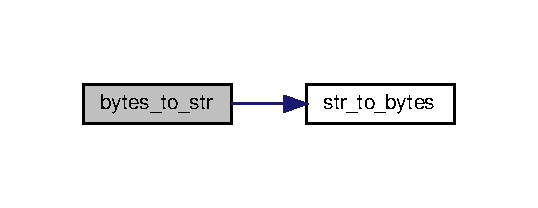
\includegraphics[width=258pt]{namespacevlc_acbb0aea5298eb7fbb31bea66b069b1b2_cgraph}
\end{center}
\end{figure}
Here is the caller graph for this function\+:
\nopagebreak
\begin{figure}[H]
\begin{center}
\leavevmode
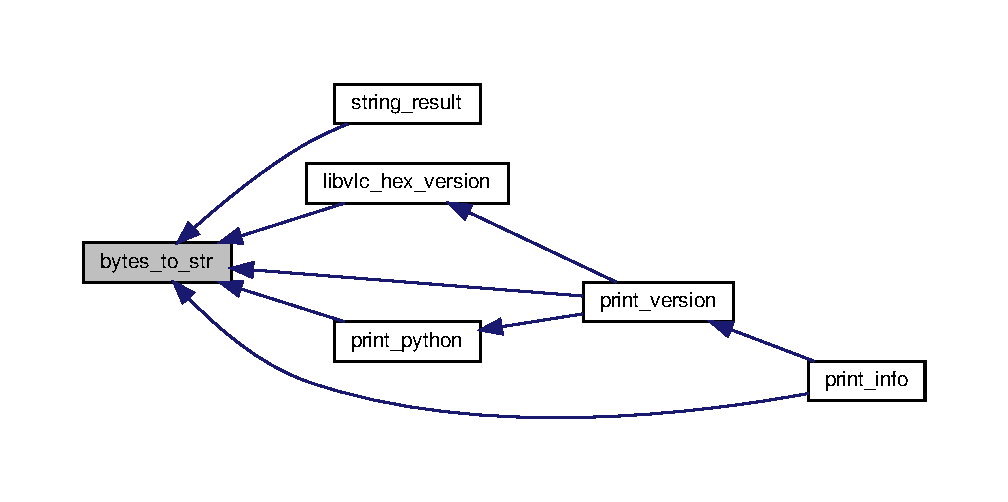
\includegraphics[width=350pt]{namespacevlc_acbb0aea5298eb7fbb31bea66b069b1b2_icgraph}
\end{center}
\end{figure}
\mbox{\Hypertarget{namespacevlc_aaddf7ebb083eb66131f099136cf6f583}\label{namespacevlc_aaddf7ebb083eb66131f099136cf6f583}} 
\index{vlc@{vlc}!callbackmethod@{callbackmethod}}
\index{callbackmethod@{callbackmethod}!vlc@{vlc}}
\subsubsection{\texorpdfstring{callbackmethod()}{callbackmethod()}}
{\footnotesize\ttfamily def vlc.\+callbackmethod (\begin{DoxyParamCaption}\item[{}]{callback }\end{DoxyParamCaption})}

\begin{DoxyVerb}Now obsolete @callbackmethod decorator.\end{DoxyVerb}
 \mbox{\Hypertarget{namespacevlc_abd89c56c1c1f69dc7c4c602ed938d5b4}\label{namespacevlc_abd89c56c1c1f69dc7c4c602ed938d5b4}} 
\index{vlc@{vlc}!class\+\_\+result@{class\+\_\+result}}
\index{class\+\_\+result@{class\+\_\+result}!vlc@{vlc}}
\subsubsection{\texorpdfstring{class\+\_\+result()}{class\_result()}}
{\footnotesize\ttfamily def vlc.\+class\+\_\+result (\begin{DoxyParamCaption}\item[{}]{classname }\end{DoxyParamCaption})}

\begin{DoxyVerb}Errcheck function. Returns a function that creates the specified class.
\end{DoxyVerb}
 Here is the caller graph for this function\+:
\nopagebreak
\begin{figure}[H]
\begin{center}
\leavevmode
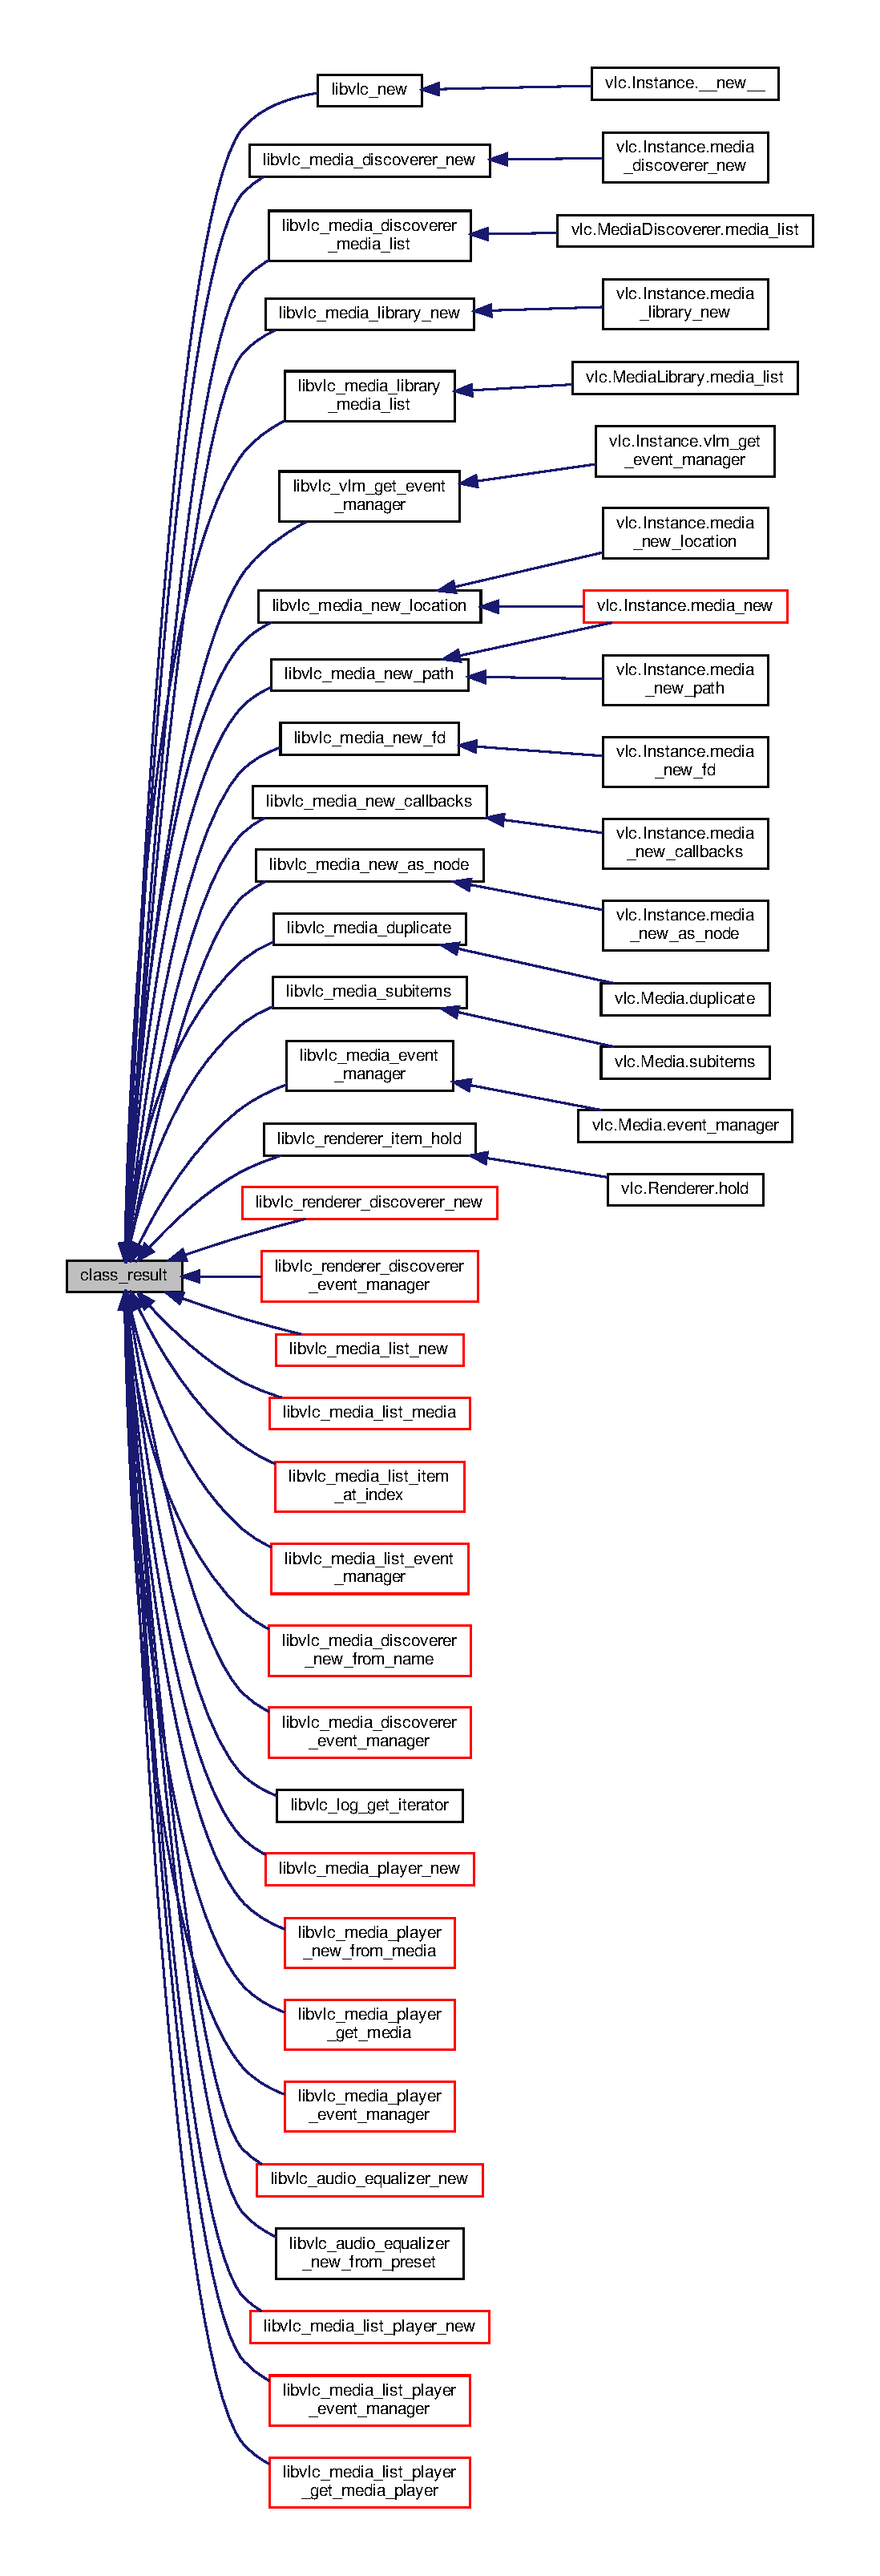
\includegraphics[height=550pt]{namespacevlc_abd89c56c1c1f69dc7c4c602ed938d5b4_icgraph}
\end{center}
\end{figure}
\mbox{\Hypertarget{namespacevlc_a14ed115618edb9fde8ca534d70c5e283}\label{namespacevlc_a14ed115618edb9fde8ca534d70c5e283}} 
\index{vlc@{vlc}!debug\+\_\+callback@{debug\+\_\+callback}}
\index{debug\+\_\+callback@{debug\+\_\+callback}!vlc@{vlc}}
\subsubsection{\texorpdfstring{debug\+\_\+callback()}{debug\_callback()}}
{\footnotesize\ttfamily def vlc.\+debug\+\_\+callback (\begin{DoxyParamCaption}\item[{}]{event,  }\item[{}]{args,  }\item[{}]{kwds }\end{DoxyParamCaption})}

\begin{DoxyVerb}Example callback, useful for debugging.
\end{DoxyVerb}
 \mbox{\Hypertarget{namespacevlc_a93ea3b472864341c8419502bd4c6a1a7}\label{namespacevlc_a93ea3b472864341c8419502bd4c6a1a7}} 
\index{vlc@{vlc}!end\+\_\+callback@{end\+\_\+callback}}
\index{end\+\_\+callback@{end\+\_\+callback}!vlc@{vlc}}
\subsubsection{\texorpdfstring{end\+\_\+callback()}{end\_callback()}}
{\footnotesize\ttfamily def vlc.\+end\+\_\+callback (\begin{DoxyParamCaption}\item[{}]{event }\end{DoxyParamCaption})}

\mbox{\Hypertarget{namespacevlc_abf92ade0b4708a70f460beddb052b761}\label{namespacevlc_abf92ade0b4708a70f460beddb052b761}} 
\index{vlc@{vlc}!find\+\_\+lib@{find\+\_\+lib}}
\index{find\+\_\+lib@{find\+\_\+lib}!vlc@{vlc}}
\subsubsection{\texorpdfstring{find\+\_\+lib()}{find\_lib()}}
{\footnotesize\ttfamily def vlc.\+find\+\_\+lib (\begin{DoxyParamCaption}{ }\end{DoxyParamCaption})}

\mbox{\Hypertarget{namespacevlc_ae7c9e2320876e2cfde006a90ff8ebd90}\label{namespacevlc_ae7c9e2320876e2cfde006a90ff8ebd90}} 
\index{vlc@{vlc}!frame\+\_\+backward@{frame\+\_\+backward}}
\index{frame\+\_\+backward@{frame\+\_\+backward}!vlc@{vlc}}
\subsubsection{\texorpdfstring{frame\+\_\+backward()}{frame\_backward()}}
{\footnotesize\ttfamily def vlc.\+frame\+\_\+backward (\begin{DoxyParamCaption}{ }\end{DoxyParamCaption})}

\begin{DoxyVerb}Go backward one frame\end{DoxyVerb}
 Here is the call graph for this function\+:
\nopagebreak
\begin{figure}[H]
\begin{center}
\leavevmode
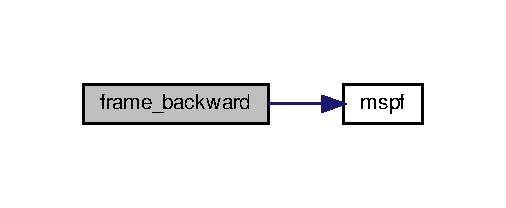
\includegraphics[width=243pt]{namespacevlc_ae7c9e2320876e2cfde006a90ff8ebd90_cgraph}
\end{center}
\end{figure}
\mbox{\Hypertarget{namespacevlc_a8ca4660553489d4345fe15e1ff1267a6}\label{namespacevlc_a8ca4660553489d4345fe15e1ff1267a6}} 
\index{vlc@{vlc}!frame\+\_\+forward@{frame\+\_\+forward}}
\index{frame\+\_\+forward@{frame\+\_\+forward}!vlc@{vlc}}
\subsubsection{\texorpdfstring{frame\+\_\+forward()}{frame\_forward()}}
{\footnotesize\ttfamily def vlc.\+frame\+\_\+forward (\begin{DoxyParamCaption}{ }\end{DoxyParamCaption})}

\begin{DoxyVerb}Go forward one frame\end{DoxyVerb}
 Here is the call graph for this function\+:
\nopagebreak
\begin{figure}[H]
\begin{center}
\leavevmode
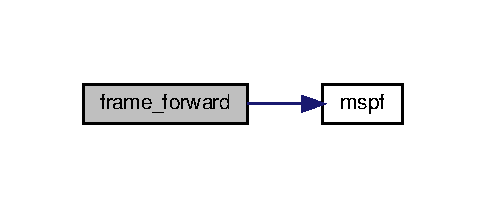
\includegraphics[width=233pt]{namespacevlc_a8ca4660553489d4345fe15e1ff1267a6_cgraph}
\end{center}
\end{figure}
\mbox{\Hypertarget{namespacevlc_a3e00cfbbf5aa7ede16e3877359d8212e}\label{namespacevlc_a3e00cfbbf5aa7ede16e3877359d8212e}} 
\index{vlc@{vlc}!get\+\_\+default\+\_\+instance@{get\+\_\+default\+\_\+instance}}
\index{get\+\_\+default\+\_\+instance@{get\+\_\+default\+\_\+instance}!vlc@{vlc}}
\subsubsection{\texorpdfstring{get\+\_\+default\+\_\+instance()}{get\_default\_instance()}}
{\footnotesize\ttfamily def vlc.\+get\+\_\+default\+\_\+instance (\begin{DoxyParamCaption}{ }\end{DoxyParamCaption})}

\begin{DoxyVerb}Return the default VLC.Instance.
\end{DoxyVerb}
 Here is the caller graph for this function\+:
\nopagebreak
\begin{figure}[H]
\begin{center}
\leavevmode
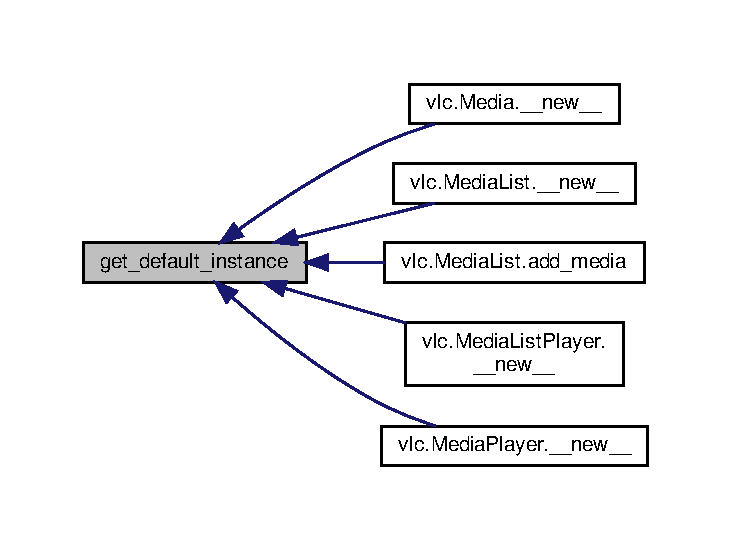
\includegraphics[width=350pt]{namespacevlc_a3e00cfbbf5aa7ede16e3877359d8212e_icgraph}
\end{center}
\end{figure}
\mbox{\Hypertarget{namespacevlc_a26c66231b8919b9ec0736a57bab415b9}\label{namespacevlc_a26c66231b8919b9ec0736a57bab415b9}} 
\index{vlc@{vlc}!getch@{getch}}
\index{getch@{getch}!vlc@{vlc}}
\subsubsection{\texorpdfstring{getch()}{getch()}}
{\footnotesize\ttfamily def vlc.\+getch (\begin{DoxyParamCaption}{ }\end{DoxyParamCaption})}

\mbox{\Hypertarget{namespacevlc_a24d18f95ac8282ca98ec1740f7f6b7cc}\label{namespacevlc_a24d18f95ac8282ca98ec1740f7f6b7cc}} 
\index{vlc@{vlc}!hex\+\_\+version@{hex\+\_\+version}}
\index{hex\+\_\+version@{hex\+\_\+version}!vlc@{vlc}}
\subsubsection{\texorpdfstring{hex\+\_\+version()}{hex\_version()}}
{\footnotesize\ttfamily def vlc.\+hex\+\_\+version (\begin{DoxyParamCaption}{ }\end{DoxyParamCaption})}

\begin{DoxyVerb}Return the version of these bindings in hex or 0 if unavailable.
\end{DoxyVerb}
 \mbox{\Hypertarget{namespacevlc_ab8767ae6377ad6875f5034a12a4cd409}\label{namespacevlc_ab8767ae6377ad6875f5034a12a4cd409}} 
\index{vlc@{vlc}!libvlc\+\_\+add\+\_\+intf@{libvlc\+\_\+add\+\_\+intf}}
\index{libvlc\+\_\+add\+\_\+intf@{libvlc\+\_\+add\+\_\+intf}!vlc@{vlc}}
\subsubsection{\texorpdfstring{libvlc\+\_\+add\+\_\+intf()}{libvlc\_add\_intf()}}
{\footnotesize\ttfamily def vlc.\+libvlc\+\_\+add\+\_\+intf (\begin{DoxyParamCaption}\item[{}]{p\+\_\+instance,  }\item[{}]{name }\end{DoxyParamCaption})}

\begin{DoxyVerb}Try to start a user interface for the libvlc instance.
@param p_instance: the instance.
@param name: interface name, or None for default.
@return: 0 on success, -1 on error.
\end{DoxyVerb}
 Here is the caller graph for this function\+:
\nopagebreak
\begin{figure}[H]
\begin{center}
\leavevmode
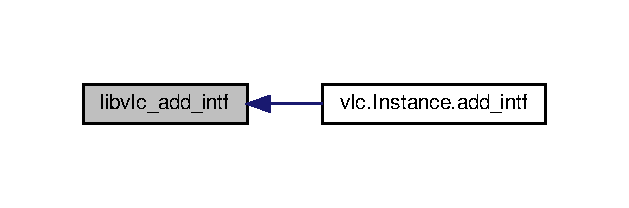
\includegraphics[width=302pt]{namespacevlc_ab8767ae6377ad6875f5034a12a4cd409_icgraph}
\end{center}
\end{figure}
\mbox{\Hypertarget{namespacevlc_ab14a271ab740aa688682202d8957f024}\label{namespacevlc_ab14a271ab740aa688682202d8957f024}} 
\index{vlc@{vlc}!libvlc\+\_\+audio\+\_\+equalizer\+\_\+get\+\_\+amp\+\_\+at\+\_\+index@{libvlc\+\_\+audio\+\_\+equalizer\+\_\+get\+\_\+amp\+\_\+at\+\_\+index}}
\index{libvlc\+\_\+audio\+\_\+equalizer\+\_\+get\+\_\+amp\+\_\+at\+\_\+index@{libvlc\+\_\+audio\+\_\+equalizer\+\_\+get\+\_\+amp\+\_\+at\+\_\+index}!vlc@{vlc}}
\subsubsection{\texorpdfstring{libvlc\+\_\+audio\+\_\+equalizer\+\_\+get\+\_\+amp\+\_\+at\+\_\+index()}{libvlc\_audio\_equalizer\_get\_amp\_at\_index()}}
{\footnotesize\ttfamily def vlc.\+libvlc\+\_\+audio\+\_\+equalizer\+\_\+get\+\_\+amp\+\_\+at\+\_\+index (\begin{DoxyParamCaption}\item[{}]{p\+\_\+equalizer,  }\item[{}]{u\+\_\+band }\end{DoxyParamCaption})}

\begin{DoxyVerb}Get the amplification value for a particular equalizer frequency band.
@param p_equalizer: valid equalizer handle, must not be None.
@param u_band: index, counting from zero, of the frequency band to get.
@return: amplification value (Hz); NaN if there is no such frequency band.
@version: LibVLC 2.2.0 or later.
\end{DoxyVerb}
 Here is the caller graph for this function\+:
\nopagebreak
\begin{figure}[H]
\begin{center}
\leavevmode
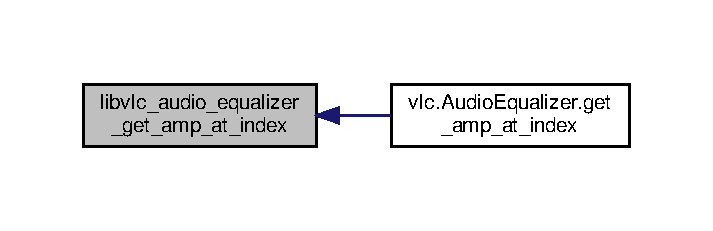
\includegraphics[width=342pt]{namespacevlc_ab14a271ab740aa688682202d8957f024_icgraph}
\end{center}
\end{figure}
\mbox{\Hypertarget{namespacevlc_ac28be065813cf41bff2b697298292012}\label{namespacevlc_ac28be065813cf41bff2b697298292012}} 
\index{vlc@{vlc}!libvlc\+\_\+audio\+\_\+equalizer\+\_\+get\+\_\+band\+\_\+count@{libvlc\+\_\+audio\+\_\+equalizer\+\_\+get\+\_\+band\+\_\+count}}
\index{libvlc\+\_\+audio\+\_\+equalizer\+\_\+get\+\_\+band\+\_\+count@{libvlc\+\_\+audio\+\_\+equalizer\+\_\+get\+\_\+band\+\_\+count}!vlc@{vlc}}
\subsubsection{\texorpdfstring{libvlc\+\_\+audio\+\_\+equalizer\+\_\+get\+\_\+band\+\_\+count()}{libvlc\_audio\_equalizer\_get\_band\_count()}}
{\footnotesize\ttfamily def vlc.\+libvlc\+\_\+audio\+\_\+equalizer\+\_\+get\+\_\+band\+\_\+count (\begin{DoxyParamCaption}{ }\end{DoxyParamCaption})}

\begin{DoxyVerb}Get the number of distinct frequency bands for an equalizer.
@return: number of frequency bands.
@version: LibVLC 2.2.0 or later.
\end{DoxyVerb}
 \mbox{\Hypertarget{namespacevlc_a14f45eb50bd638168970304368353603}\label{namespacevlc_a14f45eb50bd638168970304368353603}} 
\index{vlc@{vlc}!libvlc\+\_\+audio\+\_\+equalizer\+\_\+get\+\_\+band\+\_\+frequency@{libvlc\+\_\+audio\+\_\+equalizer\+\_\+get\+\_\+band\+\_\+frequency}}
\index{libvlc\+\_\+audio\+\_\+equalizer\+\_\+get\+\_\+band\+\_\+frequency@{libvlc\+\_\+audio\+\_\+equalizer\+\_\+get\+\_\+band\+\_\+frequency}!vlc@{vlc}}
\subsubsection{\texorpdfstring{libvlc\+\_\+audio\+\_\+equalizer\+\_\+get\+\_\+band\+\_\+frequency()}{libvlc\_audio\_equalizer\_get\_band\_frequency()}}
{\footnotesize\ttfamily def vlc.\+libvlc\+\_\+audio\+\_\+equalizer\+\_\+get\+\_\+band\+\_\+frequency (\begin{DoxyParamCaption}\item[{}]{u\+\_\+index }\end{DoxyParamCaption})}

\begin{DoxyVerb}Get a particular equalizer band frequency.
This value can be used, for example, to create a label for an equalizer band control
in a user interface.
@param u_index: index of the band, counting from zero.
@return: equalizer band frequency (Hz), or -1 if there is no such band.
@version: LibVLC 2.2.0 or later.
\end{DoxyVerb}
 \mbox{\Hypertarget{namespacevlc_a0f558cf51d137d01323634077b0f4b4e}\label{namespacevlc_a0f558cf51d137d01323634077b0f4b4e}} 
\index{vlc@{vlc}!libvlc\+\_\+audio\+\_\+equalizer\+\_\+get\+\_\+preamp@{libvlc\+\_\+audio\+\_\+equalizer\+\_\+get\+\_\+preamp}}
\index{libvlc\+\_\+audio\+\_\+equalizer\+\_\+get\+\_\+preamp@{libvlc\+\_\+audio\+\_\+equalizer\+\_\+get\+\_\+preamp}!vlc@{vlc}}
\subsubsection{\texorpdfstring{libvlc\+\_\+audio\+\_\+equalizer\+\_\+get\+\_\+preamp()}{libvlc\_audio\_equalizer\_get\_preamp()}}
{\footnotesize\ttfamily def vlc.\+libvlc\+\_\+audio\+\_\+equalizer\+\_\+get\+\_\+preamp (\begin{DoxyParamCaption}\item[{}]{p\+\_\+equalizer }\end{DoxyParamCaption})}

\begin{DoxyVerb}Get the current pre-amplification value from an equalizer.
@param p_equalizer: valid equalizer handle, must not be None.
@return: preamp value (Hz).
@version: LibVLC 2.2.0 or later.
\end{DoxyVerb}
 Here is the caller graph for this function\+:
\nopagebreak
\begin{figure}[H]
\begin{center}
\leavevmode
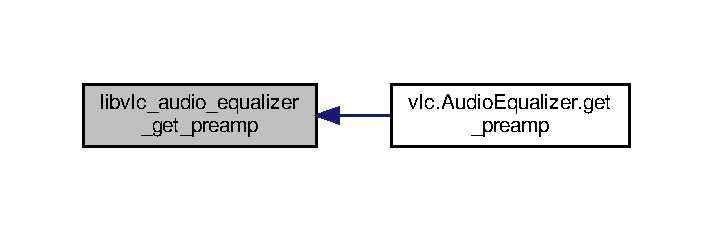
\includegraphics[width=342pt]{namespacevlc_a0f558cf51d137d01323634077b0f4b4e_icgraph}
\end{center}
\end{figure}
\mbox{\Hypertarget{namespacevlc_a8cabffd55794bdd6207aafcebaaba562}\label{namespacevlc_a8cabffd55794bdd6207aafcebaaba562}} 
\index{vlc@{vlc}!libvlc\+\_\+audio\+\_\+equalizer\+\_\+get\+\_\+preset\+\_\+count@{libvlc\+\_\+audio\+\_\+equalizer\+\_\+get\+\_\+preset\+\_\+count}}
\index{libvlc\+\_\+audio\+\_\+equalizer\+\_\+get\+\_\+preset\+\_\+count@{libvlc\+\_\+audio\+\_\+equalizer\+\_\+get\+\_\+preset\+\_\+count}!vlc@{vlc}}
\subsubsection{\texorpdfstring{libvlc\+\_\+audio\+\_\+equalizer\+\_\+get\+\_\+preset\+\_\+count()}{libvlc\_audio\_equalizer\_get\_preset\_count()}}
{\footnotesize\ttfamily def vlc.\+libvlc\+\_\+audio\+\_\+equalizer\+\_\+get\+\_\+preset\+\_\+count (\begin{DoxyParamCaption}{ }\end{DoxyParamCaption})}

\begin{DoxyVerb}Get the number of equalizer presets.
@return: number of presets.
@version: LibVLC 2.2.0 or later.
\end{DoxyVerb}
 \mbox{\Hypertarget{namespacevlc_a77eb7037c0e4a29b89dc541b0fac240d}\label{namespacevlc_a77eb7037c0e4a29b89dc541b0fac240d}} 
\index{vlc@{vlc}!libvlc\+\_\+audio\+\_\+equalizer\+\_\+get\+\_\+preset\+\_\+name@{libvlc\+\_\+audio\+\_\+equalizer\+\_\+get\+\_\+preset\+\_\+name}}
\index{libvlc\+\_\+audio\+\_\+equalizer\+\_\+get\+\_\+preset\+\_\+name@{libvlc\+\_\+audio\+\_\+equalizer\+\_\+get\+\_\+preset\+\_\+name}!vlc@{vlc}}
\subsubsection{\texorpdfstring{libvlc\+\_\+audio\+\_\+equalizer\+\_\+get\+\_\+preset\+\_\+name()}{libvlc\_audio\_equalizer\_get\_preset\_name()}}
{\footnotesize\ttfamily def vlc.\+libvlc\+\_\+audio\+\_\+equalizer\+\_\+get\+\_\+preset\+\_\+name (\begin{DoxyParamCaption}\item[{}]{u\+\_\+index }\end{DoxyParamCaption})}

\begin{DoxyVerb}Get the name of a particular equalizer preset.
This name can be used, for example, to prepare a preset label or menu in a user
interface.
@param u_index: index of the preset, counting from zero.
@return: preset name, or None if there is no such preset.
@version: LibVLC 2.2.0 or later.
\end{DoxyVerb}
 \mbox{\Hypertarget{namespacevlc_a12209b15e0da9a0481e4f7571f617dda}\label{namespacevlc_a12209b15e0da9a0481e4f7571f617dda}} 
\index{vlc@{vlc}!libvlc\+\_\+audio\+\_\+equalizer\+\_\+new@{libvlc\+\_\+audio\+\_\+equalizer\+\_\+new}}
\index{libvlc\+\_\+audio\+\_\+equalizer\+\_\+new@{libvlc\+\_\+audio\+\_\+equalizer\+\_\+new}!vlc@{vlc}}
\subsubsection{\texorpdfstring{libvlc\+\_\+audio\+\_\+equalizer\+\_\+new()}{libvlc\_audio\_equalizer\_new()}}
{\footnotesize\ttfamily def vlc.\+libvlc\+\_\+audio\+\_\+equalizer\+\_\+new (\begin{DoxyParamCaption}{ }\end{DoxyParamCaption})}

\begin{DoxyVerb}Create a new default equalizer, with all frequency values zeroed.
The new equalizer can subsequently be applied to a media player by invoking
L{libvlc_media_player_set_equalizer}().
The returned handle should be freed via L{libvlc_audio_equalizer_release}() when
it is no longer needed.
@return: opaque equalizer handle, or None on error.
@version: LibVLC 2.2.0 or later.
\end{DoxyVerb}
 Here is the call graph for this function\+:
\nopagebreak
\begin{figure}[H]
\begin{center}
\leavevmode
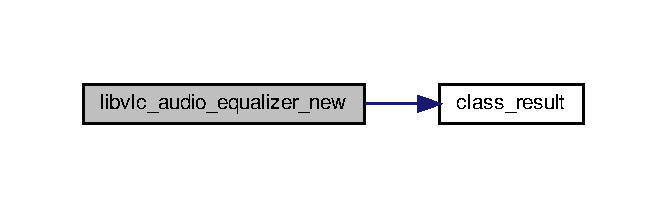
\includegraphics[width=320pt]{namespacevlc_a12209b15e0da9a0481e4f7571f617dda_cgraph}
\end{center}
\end{figure}
Here is the caller graph for this function\+:
\nopagebreak
\begin{figure}[H]
\begin{center}
\leavevmode
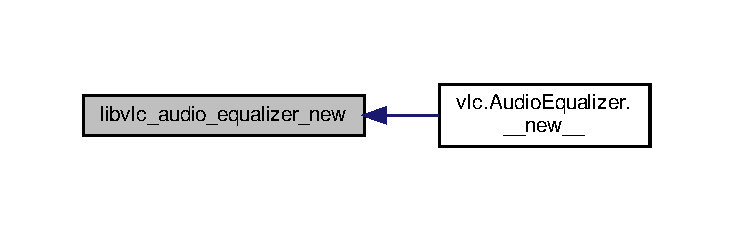
\includegraphics[width=350pt]{namespacevlc_a12209b15e0da9a0481e4f7571f617dda_icgraph}
\end{center}
\end{figure}
\mbox{\Hypertarget{namespacevlc_aeaf5e53ef0f358b71fc1796b0bc0a114}\label{namespacevlc_aeaf5e53ef0f358b71fc1796b0bc0a114}} 
\index{vlc@{vlc}!libvlc\+\_\+audio\+\_\+equalizer\+\_\+new\+\_\+from\+\_\+preset@{libvlc\+\_\+audio\+\_\+equalizer\+\_\+new\+\_\+from\+\_\+preset}}
\index{libvlc\+\_\+audio\+\_\+equalizer\+\_\+new\+\_\+from\+\_\+preset@{libvlc\+\_\+audio\+\_\+equalizer\+\_\+new\+\_\+from\+\_\+preset}!vlc@{vlc}}
\subsubsection{\texorpdfstring{libvlc\+\_\+audio\+\_\+equalizer\+\_\+new\+\_\+from\+\_\+preset()}{libvlc\_audio\_equalizer\_new\_from\_preset()}}
{\footnotesize\ttfamily def vlc.\+libvlc\+\_\+audio\+\_\+equalizer\+\_\+new\+\_\+from\+\_\+preset (\begin{DoxyParamCaption}\item[{}]{u\+\_\+index }\end{DoxyParamCaption})}

\begin{DoxyVerb}Create a new equalizer, with initial frequency values copied from an existing
preset.
The new equalizer can subsequently be applied to a media player by invoking
L{libvlc_media_player_set_equalizer}().
The returned handle should be freed via L{libvlc_audio_equalizer_release}() when
it is no longer needed.
@param u_index: index of the preset, counting from zero.
@return: opaque equalizer handle, or None on error.
@version: LibVLC 2.2.0 or later.
\end{DoxyVerb}
 Here is the call graph for this function\+:
\nopagebreak
\begin{figure}[H]
\begin{center}
\leavevmode
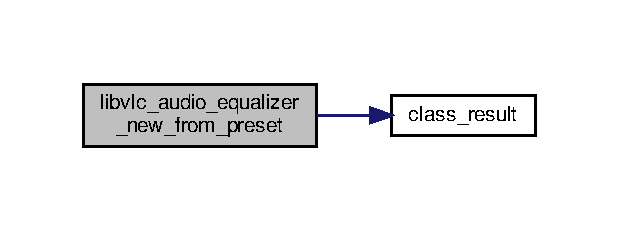
\includegraphics[width=297pt]{namespacevlc_aeaf5e53ef0f358b71fc1796b0bc0a114_cgraph}
\end{center}
\end{figure}
\mbox{\Hypertarget{namespacevlc_ae82eed728fae30f533e3bdaaeeb2fb24}\label{namespacevlc_ae82eed728fae30f533e3bdaaeeb2fb24}} 
\index{vlc@{vlc}!libvlc\+\_\+audio\+\_\+equalizer\+\_\+release@{libvlc\+\_\+audio\+\_\+equalizer\+\_\+release}}
\index{libvlc\+\_\+audio\+\_\+equalizer\+\_\+release@{libvlc\+\_\+audio\+\_\+equalizer\+\_\+release}!vlc@{vlc}}
\subsubsection{\texorpdfstring{libvlc\+\_\+audio\+\_\+equalizer\+\_\+release()}{libvlc\_audio\_equalizer\_release()}}
{\footnotesize\ttfamily def vlc.\+libvlc\+\_\+audio\+\_\+equalizer\+\_\+release (\begin{DoxyParamCaption}\item[{}]{p\+\_\+equalizer }\end{DoxyParamCaption})}

\begin{DoxyVerb}Release a previously created equalizer instance.
The equalizer was previously created by using L{libvlc_audio_equalizer_new}() or
L{libvlc_audio_equalizer_new_from_preset}().
It is safe to invoke this method with a None p_equalizer parameter for no effect.
@param p_equalizer: opaque equalizer handle, or None.
@version: LibVLC 2.2.0 or later.
\end{DoxyVerb}
 Here is the caller graph for this function\+:
\nopagebreak
\begin{figure}[H]
\begin{center}
\leavevmode
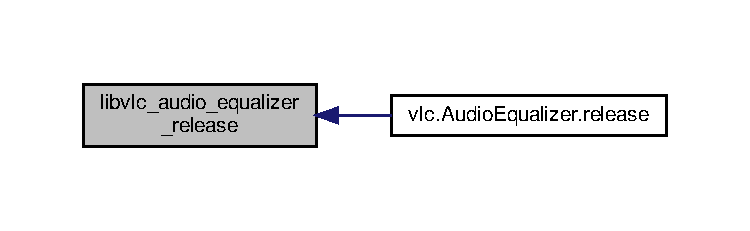
\includegraphics[width=350pt]{namespacevlc_ae82eed728fae30f533e3bdaaeeb2fb24_icgraph}
\end{center}
\end{figure}
\mbox{\Hypertarget{namespacevlc_afa112c9fa2e01582526543f4cc824132}\label{namespacevlc_afa112c9fa2e01582526543f4cc824132}} 
\index{vlc@{vlc}!libvlc\+\_\+audio\+\_\+equalizer\+\_\+set\+\_\+amp\+\_\+at\+\_\+index@{libvlc\+\_\+audio\+\_\+equalizer\+\_\+set\+\_\+amp\+\_\+at\+\_\+index}}
\index{libvlc\+\_\+audio\+\_\+equalizer\+\_\+set\+\_\+amp\+\_\+at\+\_\+index@{libvlc\+\_\+audio\+\_\+equalizer\+\_\+set\+\_\+amp\+\_\+at\+\_\+index}!vlc@{vlc}}
\subsubsection{\texorpdfstring{libvlc\+\_\+audio\+\_\+equalizer\+\_\+set\+\_\+amp\+\_\+at\+\_\+index()}{libvlc\_audio\_equalizer\_set\_amp\_at\_index()}}
{\footnotesize\ttfamily def vlc.\+libvlc\+\_\+audio\+\_\+equalizer\+\_\+set\+\_\+amp\+\_\+at\+\_\+index (\begin{DoxyParamCaption}\item[{}]{p\+\_\+equalizer,  }\item[{}]{f\+\_\+amp,  }\item[{}]{u\+\_\+band }\end{DoxyParamCaption})}

\begin{DoxyVerb}Set a new amplification value for a particular equalizer frequency band.
The new equalizer settings are subsequently applied to a media player by invoking
L{libvlc_media_player_set_equalizer}().
The supplied amplification value will be clamped to the -20.0 to +20.0 range.
@param p_equalizer: valid equalizer handle, must not be None.
@param f_amp: amplification value (-20.0 to 20.0 Hz).
@param u_band: index, counting from zero, of the frequency band to set.
@return: zero on success, -1 on error.
@version: LibVLC 2.2.0 or later.
\end{DoxyVerb}
 Here is the caller graph for this function\+:
\nopagebreak
\begin{figure}[H]
\begin{center}
\leavevmode
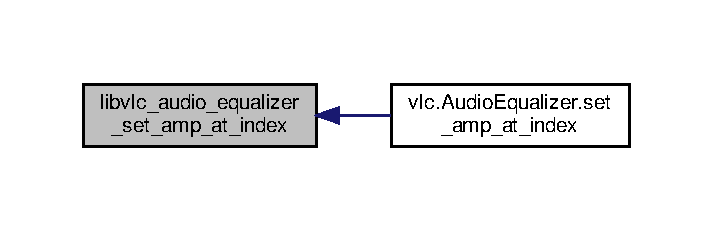
\includegraphics[width=342pt]{namespacevlc_afa112c9fa2e01582526543f4cc824132_icgraph}
\end{center}
\end{figure}
\mbox{\Hypertarget{namespacevlc_a10afe2e2760d5e0929afd7544bd08fc7}\label{namespacevlc_a10afe2e2760d5e0929afd7544bd08fc7}} 
\index{vlc@{vlc}!libvlc\+\_\+audio\+\_\+equalizer\+\_\+set\+\_\+preamp@{libvlc\+\_\+audio\+\_\+equalizer\+\_\+set\+\_\+preamp}}
\index{libvlc\+\_\+audio\+\_\+equalizer\+\_\+set\+\_\+preamp@{libvlc\+\_\+audio\+\_\+equalizer\+\_\+set\+\_\+preamp}!vlc@{vlc}}
\subsubsection{\texorpdfstring{libvlc\+\_\+audio\+\_\+equalizer\+\_\+set\+\_\+preamp()}{libvlc\_audio\_equalizer\_set\_preamp()}}
{\footnotesize\ttfamily def vlc.\+libvlc\+\_\+audio\+\_\+equalizer\+\_\+set\+\_\+preamp (\begin{DoxyParamCaption}\item[{}]{p\+\_\+equalizer,  }\item[{}]{f\+\_\+preamp }\end{DoxyParamCaption})}

\begin{DoxyVerb}Set a new pre-amplification value for an equalizer.
The new equalizer settings are subsequently applied to a media player by invoking
L{libvlc_media_player_set_equalizer}().
The supplied amplification value will be clamped to the -20.0 to +20.0 range.
@param p_equalizer: valid equalizer handle, must not be None.
@param f_preamp: preamp value (-20.0 to 20.0 Hz).
@return: zero on success, -1 on error.
@version: LibVLC 2.2.0 or later.
\end{DoxyVerb}
 Here is the caller graph for this function\+:
\nopagebreak
\begin{figure}[H]
\begin{center}
\leavevmode
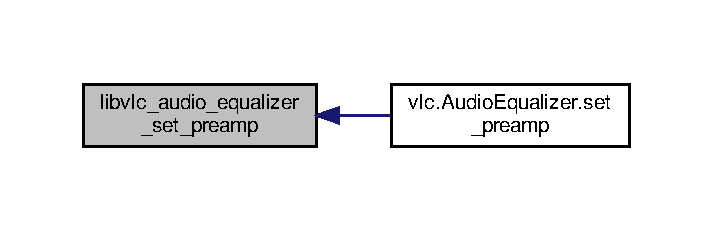
\includegraphics[width=342pt]{namespacevlc_a10afe2e2760d5e0929afd7544bd08fc7_icgraph}
\end{center}
\end{figure}
\mbox{\Hypertarget{namespacevlc_aff772ccc6681b4466b87298f076e20f5}\label{namespacevlc_aff772ccc6681b4466b87298f076e20f5}} 
\index{vlc@{vlc}!libvlc\+\_\+audio\+\_\+filter\+\_\+list\+\_\+get@{libvlc\+\_\+audio\+\_\+filter\+\_\+list\+\_\+get}}
\index{libvlc\+\_\+audio\+\_\+filter\+\_\+list\+\_\+get@{libvlc\+\_\+audio\+\_\+filter\+\_\+list\+\_\+get}!vlc@{vlc}}
\subsubsection{\texorpdfstring{libvlc\+\_\+audio\+\_\+filter\+\_\+list\+\_\+get()}{libvlc\_audio\_filter\_list\_get()}}
{\footnotesize\ttfamily def vlc.\+libvlc\+\_\+audio\+\_\+filter\+\_\+list\+\_\+get (\begin{DoxyParamCaption}\item[{}]{p\+\_\+instance }\end{DoxyParamCaption})}

\begin{DoxyVerb}Returns a list of audio filters that are available.
@param p_instance: libvlc instance.
@return: a list of module descriptions. It should be freed with L{libvlc_module_description_list_release}(). In case of an error, None is returned. See L{ModuleDescription} See L{libvlc_module_description_list_release}.
\end{DoxyVerb}
 Here is the caller graph for this function\+:
\nopagebreak
\begin{figure}[H]
\begin{center}
\leavevmode
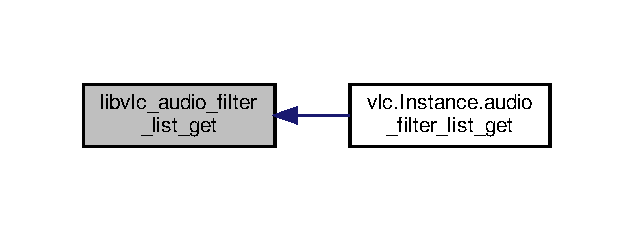
\includegraphics[width=304pt]{namespacevlc_aff772ccc6681b4466b87298f076e20f5_icgraph}
\end{center}
\end{figure}
\mbox{\Hypertarget{namespacevlc_aaea673f933311af160dd682a91e0cd89}\label{namespacevlc_aaea673f933311af160dd682a91e0cd89}} 
\index{vlc@{vlc}!libvlc\+\_\+audio\+\_\+get\+\_\+channel@{libvlc\+\_\+audio\+\_\+get\+\_\+channel}}
\index{libvlc\+\_\+audio\+\_\+get\+\_\+channel@{libvlc\+\_\+audio\+\_\+get\+\_\+channel}!vlc@{vlc}}
\subsubsection{\texorpdfstring{libvlc\+\_\+audio\+\_\+get\+\_\+channel()}{libvlc\_audio\_get\_channel()}}
{\footnotesize\ttfamily def vlc.\+libvlc\+\_\+audio\+\_\+get\+\_\+channel (\begin{DoxyParamCaption}\item[{}]{p\+\_\+mi }\end{DoxyParamCaption})}

\begin{DoxyVerb}Get current audio channel.
@param p_mi: media player.
@return: the audio channel See L{AudioOutputChannel}.
\end{DoxyVerb}
 Here is the caller graph for this function\+:
\nopagebreak
\begin{figure}[H]
\begin{center}
\leavevmode
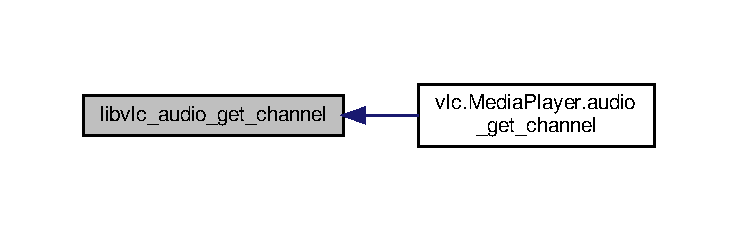
\includegraphics[width=350pt]{namespacevlc_aaea673f933311af160dd682a91e0cd89_icgraph}
\end{center}
\end{figure}
\mbox{\Hypertarget{namespacevlc_a62ec4fd04e704236c3bb48f2bada26e1}\label{namespacevlc_a62ec4fd04e704236c3bb48f2bada26e1}} 
\index{vlc@{vlc}!libvlc\+\_\+audio\+\_\+get\+\_\+delay@{libvlc\+\_\+audio\+\_\+get\+\_\+delay}}
\index{libvlc\+\_\+audio\+\_\+get\+\_\+delay@{libvlc\+\_\+audio\+\_\+get\+\_\+delay}!vlc@{vlc}}
\subsubsection{\texorpdfstring{libvlc\+\_\+audio\+\_\+get\+\_\+delay()}{libvlc\_audio\_get\_delay()}}
{\footnotesize\ttfamily def vlc.\+libvlc\+\_\+audio\+\_\+get\+\_\+delay (\begin{DoxyParamCaption}\item[{}]{p\+\_\+mi }\end{DoxyParamCaption})}

\begin{DoxyVerb}Get current audio delay.
@param p_mi: media player.
@return: the audio delay (microseconds).
@version: LibVLC 1.1.1 or later.
\end{DoxyVerb}
 Here is the caller graph for this function\+:
\nopagebreak
\begin{figure}[H]
\begin{center}
\leavevmode
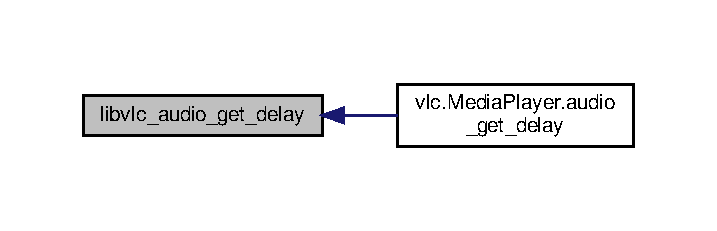
\includegraphics[width=344pt]{namespacevlc_a62ec4fd04e704236c3bb48f2bada26e1_icgraph}
\end{center}
\end{figure}
\mbox{\Hypertarget{namespacevlc_a4cdfbd29f8712d56aed3fa83b76a1b56}\label{namespacevlc_a4cdfbd29f8712d56aed3fa83b76a1b56}} 
\index{vlc@{vlc}!libvlc\+\_\+audio\+\_\+get\+\_\+mute@{libvlc\+\_\+audio\+\_\+get\+\_\+mute}}
\index{libvlc\+\_\+audio\+\_\+get\+\_\+mute@{libvlc\+\_\+audio\+\_\+get\+\_\+mute}!vlc@{vlc}}
\subsubsection{\texorpdfstring{libvlc\+\_\+audio\+\_\+get\+\_\+mute()}{libvlc\_audio\_get\_mute()}}
{\footnotesize\ttfamily def vlc.\+libvlc\+\_\+audio\+\_\+get\+\_\+mute (\begin{DoxyParamCaption}\item[{}]{p\+\_\+mi }\end{DoxyParamCaption})}

\begin{DoxyVerb}Get current mute status.
@param p_mi: media player.
@return: the mute status (boolean) if defined, -1 if undefined/unapplicable.
\end{DoxyVerb}
 Here is the caller graph for this function\+:
\nopagebreak
\begin{figure}[H]
\begin{center}
\leavevmode
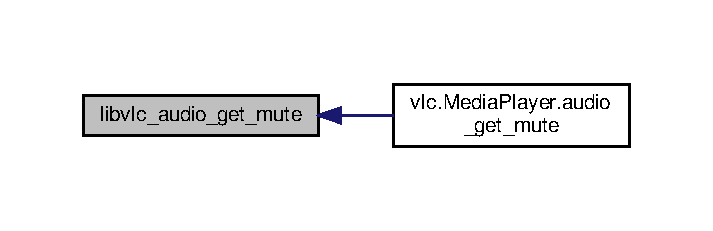
\includegraphics[width=342pt]{namespacevlc_a4cdfbd29f8712d56aed3fa83b76a1b56_icgraph}
\end{center}
\end{figure}
\mbox{\Hypertarget{namespacevlc_aacb5cb891887883b6969a152656bfb75}\label{namespacevlc_aacb5cb891887883b6969a152656bfb75}} 
\index{vlc@{vlc}!libvlc\+\_\+audio\+\_\+get\+\_\+track@{libvlc\+\_\+audio\+\_\+get\+\_\+track}}
\index{libvlc\+\_\+audio\+\_\+get\+\_\+track@{libvlc\+\_\+audio\+\_\+get\+\_\+track}!vlc@{vlc}}
\subsubsection{\texorpdfstring{libvlc\+\_\+audio\+\_\+get\+\_\+track()}{libvlc\_audio\_get\_track()}}
{\footnotesize\ttfamily def vlc.\+libvlc\+\_\+audio\+\_\+get\+\_\+track (\begin{DoxyParamCaption}\item[{}]{p\+\_\+mi }\end{DoxyParamCaption})}

\begin{DoxyVerb}Get current audio track.
@param p_mi: media player.
@return: the audio track ID or -1 if no active input.
\end{DoxyVerb}
 Here is the caller graph for this function\+:
\nopagebreak
\begin{figure}[H]
\begin{center}
\leavevmode
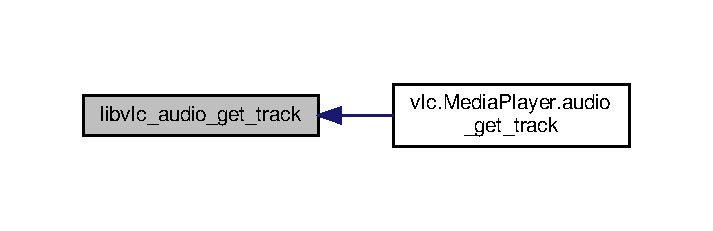
\includegraphics[width=342pt]{namespacevlc_aacb5cb891887883b6969a152656bfb75_icgraph}
\end{center}
\end{figure}
\mbox{\Hypertarget{namespacevlc_a7a1549dd2aa2d4cbd98a3fcc8da9cb09}\label{namespacevlc_a7a1549dd2aa2d4cbd98a3fcc8da9cb09}} 
\index{vlc@{vlc}!libvlc\+\_\+audio\+\_\+get\+\_\+track\+\_\+count@{libvlc\+\_\+audio\+\_\+get\+\_\+track\+\_\+count}}
\index{libvlc\+\_\+audio\+\_\+get\+\_\+track\+\_\+count@{libvlc\+\_\+audio\+\_\+get\+\_\+track\+\_\+count}!vlc@{vlc}}
\subsubsection{\texorpdfstring{libvlc\+\_\+audio\+\_\+get\+\_\+track\+\_\+count()}{libvlc\_audio\_get\_track\_count()}}
{\footnotesize\ttfamily def vlc.\+libvlc\+\_\+audio\+\_\+get\+\_\+track\+\_\+count (\begin{DoxyParamCaption}\item[{}]{p\+\_\+mi }\end{DoxyParamCaption})}

\begin{DoxyVerb}Get number of available audio tracks.
@param p_mi: media player.
@return: the number of available audio tracks (int), or -1 if unavailable.
\end{DoxyVerb}
 Here is the caller graph for this function\+:
\nopagebreak
\begin{figure}[H]
\begin{center}
\leavevmode
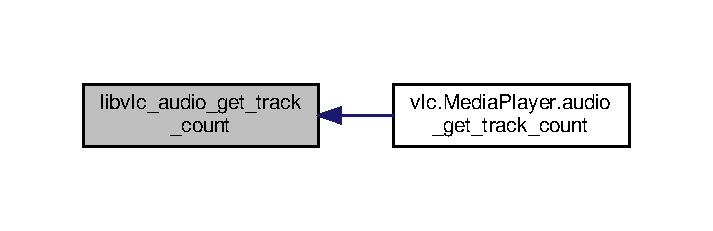
\includegraphics[width=342pt]{namespacevlc_a7a1549dd2aa2d4cbd98a3fcc8da9cb09_icgraph}
\end{center}
\end{figure}
\mbox{\Hypertarget{namespacevlc_aeef886dffdb2d28ef62fb5a2314c69b3}\label{namespacevlc_aeef886dffdb2d28ef62fb5a2314c69b3}} 
\index{vlc@{vlc}!libvlc\+\_\+audio\+\_\+get\+\_\+track\+\_\+description@{libvlc\+\_\+audio\+\_\+get\+\_\+track\+\_\+description}}
\index{libvlc\+\_\+audio\+\_\+get\+\_\+track\+\_\+description@{libvlc\+\_\+audio\+\_\+get\+\_\+track\+\_\+description}!vlc@{vlc}}
\subsubsection{\texorpdfstring{libvlc\+\_\+audio\+\_\+get\+\_\+track\+\_\+description()}{libvlc\_audio\_get\_track\_description()}}
{\footnotesize\ttfamily def vlc.\+libvlc\+\_\+audio\+\_\+get\+\_\+track\+\_\+description (\begin{DoxyParamCaption}\item[{}]{p\+\_\+mi }\end{DoxyParamCaption})}

\begin{DoxyVerb}Get the description of available audio tracks.
@param p_mi: media player.
@return: list with description of available audio tracks, or None. It must be freed with L{libvlc_track_description_list_release}().
\end{DoxyVerb}
 Here is the caller graph for this function\+:
\nopagebreak
\begin{figure}[H]
\begin{center}
\leavevmode
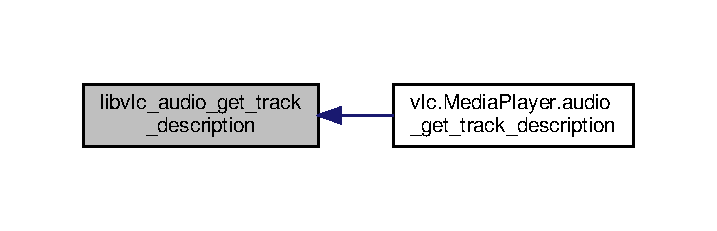
\includegraphics[width=344pt]{namespacevlc_aeef886dffdb2d28ef62fb5a2314c69b3_icgraph}
\end{center}
\end{figure}
\mbox{\Hypertarget{namespacevlc_a5bd4ab471d93bb2285affbfb6b865010}\label{namespacevlc_a5bd4ab471d93bb2285affbfb6b865010}} 
\index{vlc@{vlc}!libvlc\+\_\+audio\+\_\+get\+\_\+volume@{libvlc\+\_\+audio\+\_\+get\+\_\+volume}}
\index{libvlc\+\_\+audio\+\_\+get\+\_\+volume@{libvlc\+\_\+audio\+\_\+get\+\_\+volume}!vlc@{vlc}}
\subsubsection{\texorpdfstring{libvlc\+\_\+audio\+\_\+get\+\_\+volume()}{libvlc\_audio\_get\_volume()}}
{\footnotesize\ttfamily def vlc.\+libvlc\+\_\+audio\+\_\+get\+\_\+volume (\begin{DoxyParamCaption}\item[{}]{p\+\_\+mi }\end{DoxyParamCaption})}

\begin{DoxyVerb}Get current software audio volume.
@param p_mi: media player.
@return: the software volume in percents (0 = mute, 100 = nominal / 0dB).
\end{DoxyVerb}
 Here is the caller graph for this function\+:
\nopagebreak
\begin{figure}[H]
\begin{center}
\leavevmode
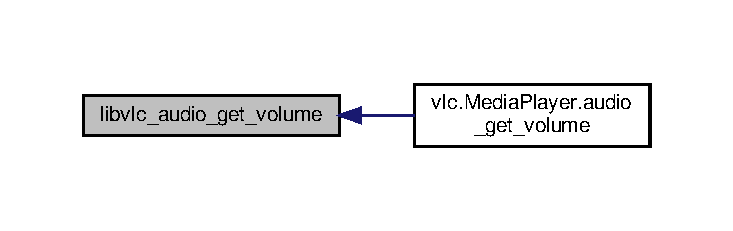
\includegraphics[width=350pt]{namespacevlc_a5bd4ab471d93bb2285affbfb6b865010_icgraph}
\end{center}
\end{figure}
\mbox{\Hypertarget{namespacevlc_ab26cd1fc475f71b8faa4e86f9c95ce21}\label{namespacevlc_ab26cd1fc475f71b8faa4e86f9c95ce21}} 
\index{vlc@{vlc}!libvlc\+\_\+audio\+\_\+output\+\_\+device\+\_\+count@{libvlc\+\_\+audio\+\_\+output\+\_\+device\+\_\+count}}
\index{libvlc\+\_\+audio\+\_\+output\+\_\+device\+\_\+count@{libvlc\+\_\+audio\+\_\+output\+\_\+device\+\_\+count}!vlc@{vlc}}
\subsubsection{\texorpdfstring{libvlc\+\_\+audio\+\_\+output\+\_\+device\+\_\+count()}{libvlc\_audio\_output\_device\_count()}}
{\footnotesize\ttfamily def vlc.\+libvlc\+\_\+audio\+\_\+output\+\_\+device\+\_\+count (\begin{DoxyParamCaption}\item[{}]{p\+\_\+instance,  }\item[{}]{psz\+\_\+audio\+\_\+output }\end{DoxyParamCaption})}

\begin{DoxyVerb}Backward compatibility stub. Do not use in new code.
\deprecated Use L{libvlc_audio_output_device_list_get}() instead.
@return: always 0.
\end{DoxyVerb}
 Here is the caller graph for this function\+:
\nopagebreak
\begin{figure}[H]
\begin{center}
\leavevmode
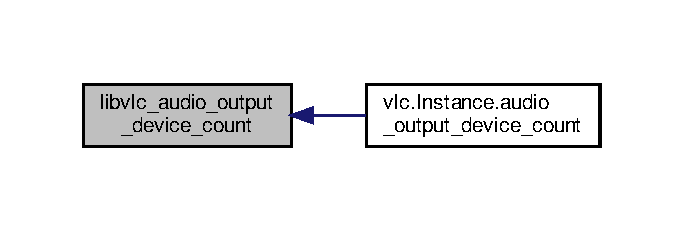
\includegraphics[width=328pt]{namespacevlc_ab26cd1fc475f71b8faa4e86f9c95ce21_icgraph}
\end{center}
\end{figure}
\mbox{\Hypertarget{namespacevlc_ad0eaa466313964c4c8f8fca0cdb4dc03}\label{namespacevlc_ad0eaa466313964c4c8f8fca0cdb4dc03}} 
\index{vlc@{vlc}!libvlc\+\_\+audio\+\_\+output\+\_\+device\+\_\+enum@{libvlc\+\_\+audio\+\_\+output\+\_\+device\+\_\+enum}}
\index{libvlc\+\_\+audio\+\_\+output\+\_\+device\+\_\+enum@{libvlc\+\_\+audio\+\_\+output\+\_\+device\+\_\+enum}!vlc@{vlc}}
\subsubsection{\texorpdfstring{libvlc\+\_\+audio\+\_\+output\+\_\+device\+\_\+enum()}{libvlc\_audio\_output\_device\_enum()}}
{\footnotesize\ttfamily def vlc.\+libvlc\+\_\+audio\+\_\+output\+\_\+device\+\_\+enum (\begin{DoxyParamCaption}\item[{}]{mp }\end{DoxyParamCaption})}

\begin{DoxyVerb}Gets a list of potential audio output devices,
See L{libvlc_audio_output_device_set}().
@note: Not all audio outputs support enumerating devices.
The audio output may be functional even if the list is empty (None).
@note: The list may not be exhaustive.
@warning: Some audio output devices in the list might not actually work in
some circumstances. By default, it is recommended to not specify any
explicit audio device.
@param mp: media player.
@return: A None-terminated linked list of potential audio output devices. It must be freed with L{libvlc_audio_output_device_list_release}().
@version: LibVLC 2.2.0 or later.
\end{DoxyVerb}
 Here is the caller graph for this function\+:
\nopagebreak
\begin{figure}[H]
\begin{center}
\leavevmode
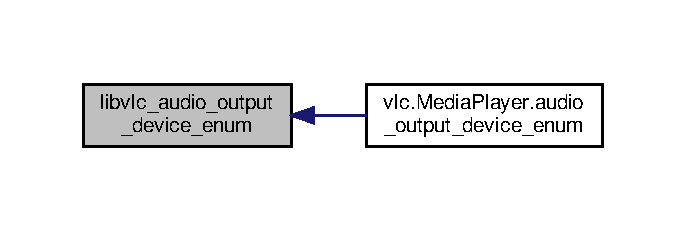
\includegraphics[width=329pt]{namespacevlc_ad0eaa466313964c4c8f8fca0cdb4dc03_icgraph}
\end{center}
\end{figure}
\mbox{\Hypertarget{namespacevlc_a5b5babcb373f2af5cfa81ff75f932192}\label{namespacevlc_a5b5babcb373f2af5cfa81ff75f932192}} 
\index{vlc@{vlc}!libvlc\+\_\+audio\+\_\+output\+\_\+device\+\_\+get@{libvlc\+\_\+audio\+\_\+output\+\_\+device\+\_\+get}}
\index{libvlc\+\_\+audio\+\_\+output\+\_\+device\+\_\+get@{libvlc\+\_\+audio\+\_\+output\+\_\+device\+\_\+get}!vlc@{vlc}}
\subsubsection{\texorpdfstring{libvlc\+\_\+audio\+\_\+output\+\_\+device\+\_\+get()}{libvlc\_audio\_output\_device\_get()}}
{\footnotesize\ttfamily def vlc.\+libvlc\+\_\+audio\+\_\+output\+\_\+device\+\_\+get (\begin{DoxyParamCaption}\item[{}]{mp }\end{DoxyParamCaption})}

\begin{DoxyVerb}Get the current audio output device identifier.
This complements L{libvlc_audio_output_device_set}().
@warning: The initial value for the current audio output device identifier
may not be set or may be some unknown value. A LibVLC application should
compare this value against the known device identifiers (e.g. those that
were previously retrieved by a call to L{libvlc_audio_output_device_enum} or
L{libvlc_audio_output_device_list_get}) to find the current audio output device.
It is possible that the selected audio output device changes (an external
change) without a call to L{libvlc_audio_output_device_set}. That may make this
method unsuitable to use if a LibVLC application is attempting to track
dynamic audio device changes as they happen.
@param mp: media player.
@return: the current audio output device identifier None if no device is selected or in case of error (the result must be released with free() or L{libvlc_free}()).
@version: LibVLC 3.0.0 or later.
\end{DoxyVerb}
 Here is the caller graph for this function\+:
\nopagebreak
\begin{figure}[H]
\begin{center}
\leavevmode
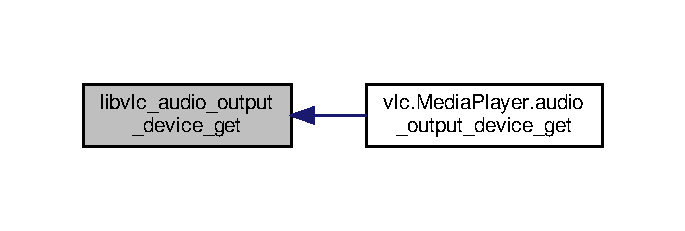
\includegraphics[width=329pt]{namespacevlc_a5b5babcb373f2af5cfa81ff75f932192_icgraph}
\end{center}
\end{figure}
\mbox{\Hypertarget{namespacevlc_a058a41cbf5946ba44fdb114876c47d81}\label{namespacevlc_a058a41cbf5946ba44fdb114876c47d81}} 
\index{vlc@{vlc}!libvlc\+\_\+audio\+\_\+output\+\_\+device\+\_\+id@{libvlc\+\_\+audio\+\_\+output\+\_\+device\+\_\+id}}
\index{libvlc\+\_\+audio\+\_\+output\+\_\+device\+\_\+id@{libvlc\+\_\+audio\+\_\+output\+\_\+device\+\_\+id}!vlc@{vlc}}
\subsubsection{\texorpdfstring{libvlc\+\_\+audio\+\_\+output\+\_\+device\+\_\+id()}{libvlc\_audio\_output\_device\_id()}}
{\footnotesize\ttfamily def vlc.\+libvlc\+\_\+audio\+\_\+output\+\_\+device\+\_\+id (\begin{DoxyParamCaption}\item[{}]{p\+\_\+instance,  }\item[{}]{psz\+\_\+audio\+\_\+output,  }\item[{}]{i\+\_\+device }\end{DoxyParamCaption})}

\begin{DoxyVerb}Backward compatibility stub. Do not use in new code.
\deprecated Use L{libvlc_audio_output_device_list_get}() instead.
@return: always None.
\end{DoxyVerb}
 Here is the caller graph for this function\+:
\nopagebreak
\begin{figure}[H]
\begin{center}
\leavevmode
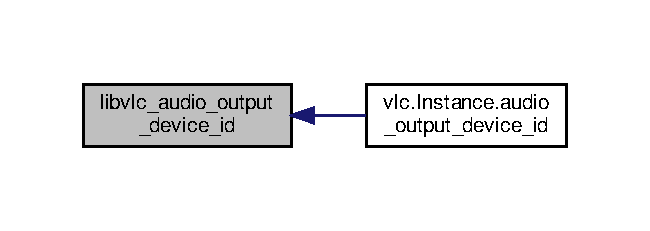
\includegraphics[width=312pt]{namespacevlc_a058a41cbf5946ba44fdb114876c47d81_icgraph}
\end{center}
\end{figure}
\mbox{\Hypertarget{namespacevlc_a398beca7c466c6dee8cf8f97dec6664e}\label{namespacevlc_a398beca7c466c6dee8cf8f97dec6664e}} 
\index{vlc@{vlc}!libvlc\+\_\+audio\+\_\+output\+\_\+device\+\_\+list\+\_\+get@{libvlc\+\_\+audio\+\_\+output\+\_\+device\+\_\+list\+\_\+get}}
\index{libvlc\+\_\+audio\+\_\+output\+\_\+device\+\_\+list\+\_\+get@{libvlc\+\_\+audio\+\_\+output\+\_\+device\+\_\+list\+\_\+get}!vlc@{vlc}}
\subsubsection{\texorpdfstring{libvlc\+\_\+audio\+\_\+output\+\_\+device\+\_\+list\+\_\+get()}{libvlc\_audio\_output\_device\_list\_get()}}
{\footnotesize\ttfamily def vlc.\+libvlc\+\_\+audio\+\_\+output\+\_\+device\+\_\+list\+\_\+get (\begin{DoxyParamCaption}\item[{}]{p\+\_\+instance,  }\item[{}]{aout }\end{DoxyParamCaption})}

\begin{DoxyVerb}Gets a list of audio output devices for a given audio output module,
See L{libvlc_audio_output_device_set}().
@note: Not all audio outputs support this. In particular, an empty (None)
list of devices does B{not} imply that the specified audio output does
not work.
@note: The list might not be exhaustive.
@warning: Some audio output devices in the list might not actually work in
some circumstances. By default, it is recommended to not specify any
explicit audio device.
@param p_instance: libvlc instance.
@param aout: audio output name (as returned by L{libvlc_audio_output_list_get}()).
@return: A None-terminated linked list of potential audio output devices. It must be freed with L{libvlc_audio_output_device_list_release}().
@version: LibVLC 2.1.0 or later.
\end{DoxyVerb}
 Here is the caller graph for this function\+:
\nopagebreak
\begin{figure}[H]
\begin{center}
\leavevmode
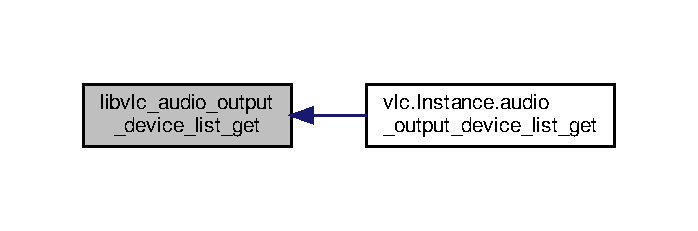
\includegraphics[width=335pt]{namespacevlc_a398beca7c466c6dee8cf8f97dec6664e_icgraph}
\end{center}
\end{figure}
\mbox{\Hypertarget{namespacevlc_a0bab07db85d9932daaa7f9bd017702eb}\label{namespacevlc_a0bab07db85d9932daaa7f9bd017702eb}} 
\index{vlc@{vlc}!libvlc\+\_\+audio\+\_\+output\+\_\+device\+\_\+list\+\_\+release@{libvlc\+\_\+audio\+\_\+output\+\_\+device\+\_\+list\+\_\+release}}
\index{libvlc\+\_\+audio\+\_\+output\+\_\+device\+\_\+list\+\_\+release@{libvlc\+\_\+audio\+\_\+output\+\_\+device\+\_\+list\+\_\+release}!vlc@{vlc}}
\subsubsection{\texorpdfstring{libvlc\+\_\+audio\+\_\+output\+\_\+device\+\_\+list\+\_\+release()}{libvlc\_audio\_output\_device\_list\_release()}}
{\footnotesize\ttfamily def vlc.\+libvlc\+\_\+audio\+\_\+output\+\_\+device\+\_\+list\+\_\+release (\begin{DoxyParamCaption}\item[{}]{p\+\_\+list }\end{DoxyParamCaption})}

\begin{DoxyVerb}Frees a list of available audio output devices.
@param p_list: list with audio outputs for release.
@version: LibVLC 2.1.0 or later.
\end{DoxyVerb}
 \mbox{\Hypertarget{namespacevlc_a88c35604ea93344aaec29a2967e5ffa8}\label{namespacevlc_a88c35604ea93344aaec29a2967e5ffa8}} 
\index{vlc@{vlc}!libvlc\+\_\+audio\+\_\+output\+\_\+device\+\_\+longname@{libvlc\+\_\+audio\+\_\+output\+\_\+device\+\_\+longname}}
\index{libvlc\+\_\+audio\+\_\+output\+\_\+device\+\_\+longname@{libvlc\+\_\+audio\+\_\+output\+\_\+device\+\_\+longname}!vlc@{vlc}}
\subsubsection{\texorpdfstring{libvlc\+\_\+audio\+\_\+output\+\_\+device\+\_\+longname()}{libvlc\_audio\_output\_device\_longname()}}
{\footnotesize\ttfamily def vlc.\+libvlc\+\_\+audio\+\_\+output\+\_\+device\+\_\+longname (\begin{DoxyParamCaption}\item[{}]{p\+\_\+instance,  }\item[{}]{psz\+\_\+output,  }\item[{}]{i\+\_\+device }\end{DoxyParamCaption})}

\begin{DoxyVerb}Backward compatibility stub. Do not use in new code.
\deprecated Use L{libvlc_audio_output_device_list_get}() instead.
@return: always None.
\end{DoxyVerb}
 Here is the caller graph for this function\+:
\nopagebreak
\begin{figure}[H]
\begin{center}
\leavevmode
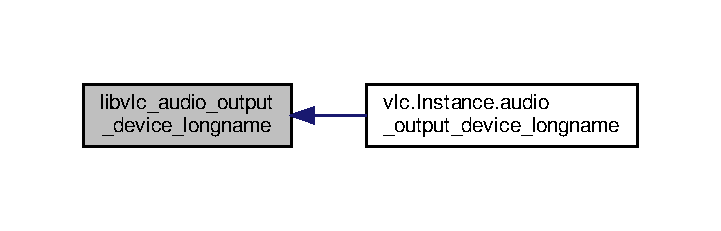
\includegraphics[width=346pt]{namespacevlc_a88c35604ea93344aaec29a2967e5ffa8_icgraph}
\end{center}
\end{figure}
\mbox{\Hypertarget{namespacevlc_a25b3f026d49515a2d0ae0906495c5fcb}\label{namespacevlc_a25b3f026d49515a2d0ae0906495c5fcb}} 
\index{vlc@{vlc}!libvlc\+\_\+audio\+\_\+output\+\_\+device\+\_\+set@{libvlc\+\_\+audio\+\_\+output\+\_\+device\+\_\+set}}
\index{libvlc\+\_\+audio\+\_\+output\+\_\+device\+\_\+set@{libvlc\+\_\+audio\+\_\+output\+\_\+device\+\_\+set}!vlc@{vlc}}
\subsubsection{\texorpdfstring{libvlc\+\_\+audio\+\_\+output\+\_\+device\+\_\+set()}{libvlc\_audio\_output\_device\_set()}}
{\footnotesize\ttfamily def vlc.\+libvlc\+\_\+audio\+\_\+output\+\_\+device\+\_\+set (\begin{DoxyParamCaption}\item[{}]{mp,  }\item[{}]{module,  }\item[{}]{device\+\_\+id }\end{DoxyParamCaption})}

\begin{DoxyVerb}Configures an explicit audio output device.
If the module paramater is None, audio output will be moved to the device
specified by the device identifier string immediately. This is the
recommended usage.
A list of adequate potential device strings can be obtained with
L{libvlc_audio_output_device_enum}().
However passing None is supported in LibVLC version 2.2.0 and later only;
in earlier versions, this function would have no effects when the module
parameter was None.
If the module parameter is not None, the device parameter of the
corresponding audio output, if it exists, will be set to the specified
string. Note that some audio output modules do not have such a parameter
(notably MMDevice and PulseAudio).
A list of adequate potential device strings can be obtained with
L{libvlc_audio_output_device_list_get}().
@note: This function does not select the specified audio output plugin.
L{libvlc_audio_output_set}() is used for that purpose.
@warning: The syntax for the device parameter depends on the audio output.
Some audio output modules require further parameters (e.g. a channels map
in the case of ALSA).
@param mp: media player.
@param module: If None, current audio output module. if non-None, name of audio output module.
@param device_id: device identifier string.
@return: Nothing. Errors are ignored (this is a design bug).
\end{DoxyVerb}
 Here is the caller graph for this function\+:
\nopagebreak
\begin{figure}[H]
\begin{center}
\leavevmode
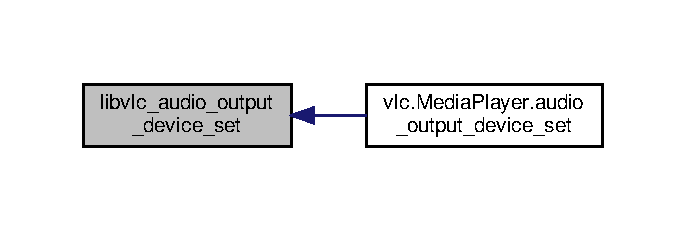
\includegraphics[width=329pt]{namespacevlc_a25b3f026d49515a2d0ae0906495c5fcb_icgraph}
\end{center}
\end{figure}
\mbox{\Hypertarget{namespacevlc_a8261ae46b9414ab68671c6c9d2799d47}\label{namespacevlc_a8261ae46b9414ab68671c6c9d2799d47}} 
\index{vlc@{vlc}!libvlc\+\_\+audio\+\_\+output\+\_\+list\+\_\+get@{libvlc\+\_\+audio\+\_\+output\+\_\+list\+\_\+get}}
\index{libvlc\+\_\+audio\+\_\+output\+\_\+list\+\_\+get@{libvlc\+\_\+audio\+\_\+output\+\_\+list\+\_\+get}!vlc@{vlc}}
\subsubsection{\texorpdfstring{libvlc\+\_\+audio\+\_\+output\+\_\+list\+\_\+get()}{libvlc\_audio\_output\_list\_get()}}
{\footnotesize\ttfamily def vlc.\+libvlc\+\_\+audio\+\_\+output\+\_\+list\+\_\+get (\begin{DoxyParamCaption}\item[{}]{p\+\_\+instance }\end{DoxyParamCaption})}

\begin{DoxyVerb}Gets the list of available audio output modules.
@param p_instance: libvlc instance.
@return: list of available audio outputs. It must be freed with In case of error, None is returned.
\end{DoxyVerb}
 Here is the caller graph for this function\+:
\nopagebreak
\begin{figure}[H]
\begin{center}
\leavevmode
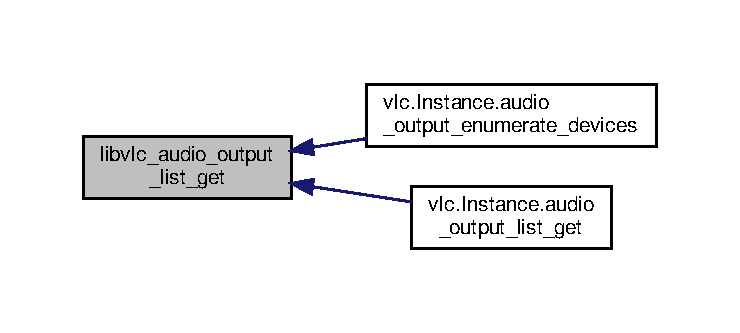
\includegraphics[width=350pt]{namespacevlc_a8261ae46b9414ab68671c6c9d2799d47_icgraph}
\end{center}
\end{figure}
\mbox{\Hypertarget{namespacevlc_aa3a70d05c0ceda7ef8abf29e5f0237bc}\label{namespacevlc_aa3a70d05c0ceda7ef8abf29e5f0237bc}} 
\index{vlc@{vlc}!libvlc\+\_\+audio\+\_\+output\+\_\+list\+\_\+release@{libvlc\+\_\+audio\+\_\+output\+\_\+list\+\_\+release}}
\index{libvlc\+\_\+audio\+\_\+output\+\_\+list\+\_\+release@{libvlc\+\_\+audio\+\_\+output\+\_\+list\+\_\+release}!vlc@{vlc}}
\subsubsection{\texorpdfstring{libvlc\+\_\+audio\+\_\+output\+\_\+list\+\_\+release()}{libvlc\_audio\_output\_list\_release()}}
{\footnotesize\ttfamily def vlc.\+libvlc\+\_\+audio\+\_\+output\+\_\+list\+\_\+release (\begin{DoxyParamCaption}\item[{}]{p\+\_\+list }\end{DoxyParamCaption})}

\begin{DoxyVerb}Frees the list of available audio output modules.
@param p_list: list with audio outputs for release.
\end{DoxyVerb}
 Here is the caller graph for this function\+:
\nopagebreak
\begin{figure}[H]
\begin{center}
\leavevmode
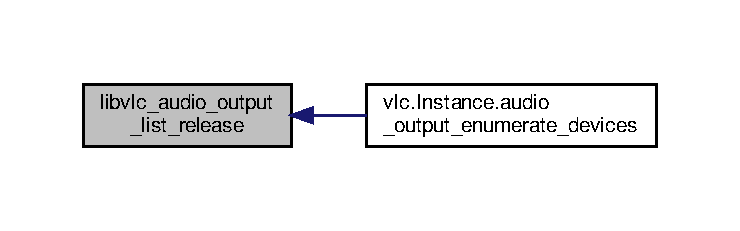
\includegraphics[width=350pt]{namespacevlc_aa3a70d05c0ceda7ef8abf29e5f0237bc_icgraph}
\end{center}
\end{figure}
\mbox{\Hypertarget{namespacevlc_a78552faa46d9cfa68ff163224b9a5c40}\label{namespacevlc_a78552faa46d9cfa68ff163224b9a5c40}} 
\index{vlc@{vlc}!libvlc\+\_\+audio\+\_\+output\+\_\+set@{libvlc\+\_\+audio\+\_\+output\+\_\+set}}
\index{libvlc\+\_\+audio\+\_\+output\+\_\+set@{libvlc\+\_\+audio\+\_\+output\+\_\+set}!vlc@{vlc}}
\subsubsection{\texorpdfstring{libvlc\+\_\+audio\+\_\+output\+\_\+set()}{libvlc\_audio\_output\_set()}}
{\footnotesize\ttfamily def vlc.\+libvlc\+\_\+audio\+\_\+output\+\_\+set (\begin{DoxyParamCaption}\item[{}]{p\+\_\+mi,  }\item[{}]{psz\+\_\+name }\end{DoxyParamCaption})}

\begin{DoxyVerb}Selects an audio output module.
@note: Any change will take be effect only after playback is stopped and
restarted. Audio output cannot be changed while playing.
@param p_mi: media player.
@param psz_name: name of audio output, use psz_name of See L{AudioOutput}.
@return: 0 if function succeeded, -1 on error.
\end{DoxyVerb}
 Here is the caller graph for this function\+:
\nopagebreak
\begin{figure}[H]
\begin{center}
\leavevmode
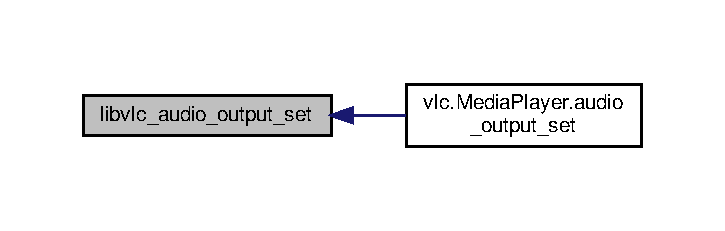
\includegraphics[width=348pt]{namespacevlc_a78552faa46d9cfa68ff163224b9a5c40_icgraph}
\end{center}
\end{figure}
\mbox{\Hypertarget{namespacevlc_a8edc679f928c8870c5412270fea57b6c}\label{namespacevlc_a8edc679f928c8870c5412270fea57b6c}} 
\index{vlc@{vlc}!libvlc\+\_\+audio\+\_\+set\+\_\+callbacks@{libvlc\+\_\+audio\+\_\+set\+\_\+callbacks}}
\index{libvlc\+\_\+audio\+\_\+set\+\_\+callbacks@{libvlc\+\_\+audio\+\_\+set\+\_\+callbacks}!vlc@{vlc}}
\subsubsection{\texorpdfstring{libvlc\+\_\+audio\+\_\+set\+\_\+callbacks()}{libvlc\_audio\_set\_callbacks()}}
{\footnotesize\ttfamily def vlc.\+libvlc\+\_\+audio\+\_\+set\+\_\+callbacks (\begin{DoxyParamCaption}\item[{}]{mp,  }\item[{}]{play,  }\item[{}]{pause,  }\item[{}]{resume,  }\item[{}]{flush,  }\item[{}]{drain,  }\item[{}]{opaque }\end{DoxyParamCaption})}

\begin{DoxyVerb}Sets callbacks and private data for decoded audio.
Use L{libvlc_audio_set_format}() or L{libvlc_audio_set_format_callbacks}()
to configure the decoded audio format.
@note: The audio callbacks override any other audio output mechanism.
If the callbacks are set, LibVLC will B{not} output audio in any way.
@param mp: the media player.
@param play: callback to play audio samples (must not be None).
@param pause: callback to pause playback (or None to ignore).
@param resume: callback to resume playback (or None to ignore).
@param flush: callback to flush audio buffers (or None to ignore).
@param drain: callback to drain audio buffers (or None to ignore).
@param opaque: private pointer for the audio callbacks (as first parameter).
@version: LibVLC 2.0.0 or later.
\end{DoxyVerb}
 Here is the caller graph for this function\+:
\nopagebreak
\begin{figure}[H]
\begin{center}
\leavevmode
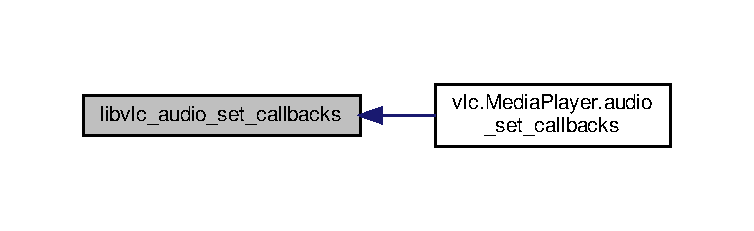
\includegraphics[width=350pt]{namespacevlc_a8edc679f928c8870c5412270fea57b6c_icgraph}
\end{center}
\end{figure}
\mbox{\Hypertarget{namespacevlc_abc0358f7a4053006f13577861532937c}\label{namespacevlc_abc0358f7a4053006f13577861532937c}} 
\index{vlc@{vlc}!libvlc\+\_\+audio\+\_\+set\+\_\+channel@{libvlc\+\_\+audio\+\_\+set\+\_\+channel}}
\index{libvlc\+\_\+audio\+\_\+set\+\_\+channel@{libvlc\+\_\+audio\+\_\+set\+\_\+channel}!vlc@{vlc}}
\subsubsection{\texorpdfstring{libvlc\+\_\+audio\+\_\+set\+\_\+channel()}{libvlc\_audio\_set\_channel()}}
{\footnotesize\ttfamily def vlc.\+libvlc\+\_\+audio\+\_\+set\+\_\+channel (\begin{DoxyParamCaption}\item[{}]{p\+\_\+mi,  }\item[{}]{channel }\end{DoxyParamCaption})}

\begin{DoxyVerb}Set current audio channel.
@param p_mi: media player.
@param channel: the audio channel, See L{AudioOutputChannel}.
@return: 0 on success, -1 on error.
\end{DoxyVerb}
 Here is the caller graph for this function\+:
\nopagebreak
\begin{figure}[H]
\begin{center}
\leavevmode
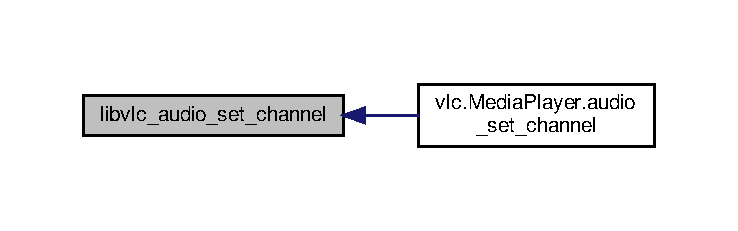
\includegraphics[width=350pt]{namespacevlc_abc0358f7a4053006f13577861532937c_icgraph}
\end{center}
\end{figure}
\mbox{\Hypertarget{namespacevlc_a4f69c99e5eaf09175dd4353d56e934d8}\label{namespacevlc_a4f69c99e5eaf09175dd4353d56e934d8}} 
\index{vlc@{vlc}!libvlc\+\_\+audio\+\_\+set\+\_\+delay@{libvlc\+\_\+audio\+\_\+set\+\_\+delay}}
\index{libvlc\+\_\+audio\+\_\+set\+\_\+delay@{libvlc\+\_\+audio\+\_\+set\+\_\+delay}!vlc@{vlc}}
\subsubsection{\texorpdfstring{libvlc\+\_\+audio\+\_\+set\+\_\+delay()}{libvlc\_audio\_set\_delay()}}
{\footnotesize\ttfamily def vlc.\+libvlc\+\_\+audio\+\_\+set\+\_\+delay (\begin{DoxyParamCaption}\item[{}]{p\+\_\+mi,  }\item[{}]{i\+\_\+delay }\end{DoxyParamCaption})}

\begin{DoxyVerb}Set current audio delay. The audio delay will be reset to zero each time the media changes.
@param p_mi: media player.
@param i_delay: the audio delay (microseconds).
@return: 0 on success, -1 on error.
@version: LibVLC 1.1.1 or later.
\end{DoxyVerb}
 Here is the caller graph for this function\+:
\nopagebreak
\begin{figure}[H]
\begin{center}
\leavevmode
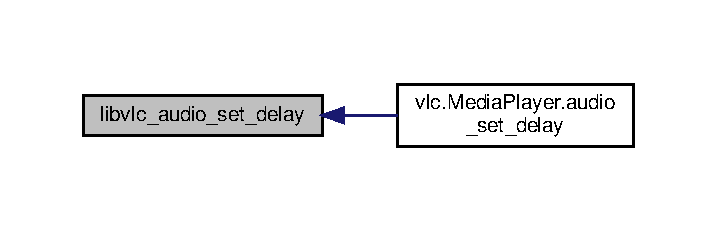
\includegraphics[width=344pt]{namespacevlc_a4f69c99e5eaf09175dd4353d56e934d8_icgraph}
\end{center}
\end{figure}
\mbox{\Hypertarget{namespacevlc_ab91a179094998e8bf3c5be9ab109e206}\label{namespacevlc_ab91a179094998e8bf3c5be9ab109e206}} 
\index{vlc@{vlc}!libvlc\+\_\+audio\+\_\+set\+\_\+format@{libvlc\+\_\+audio\+\_\+set\+\_\+format}}
\index{libvlc\+\_\+audio\+\_\+set\+\_\+format@{libvlc\+\_\+audio\+\_\+set\+\_\+format}!vlc@{vlc}}
\subsubsection{\texorpdfstring{libvlc\+\_\+audio\+\_\+set\+\_\+format()}{libvlc\_audio\_set\_format()}}
{\footnotesize\ttfamily def vlc.\+libvlc\+\_\+audio\+\_\+set\+\_\+format (\begin{DoxyParamCaption}\item[{}]{mp,  }\item[{}]{format,  }\item[{}]{rate,  }\item[{}]{channels }\end{DoxyParamCaption})}

\begin{DoxyVerb}Sets a fixed decoded audio format.
This only works in combination with L{libvlc_audio_set_callbacks}(),
and is mutually exclusive with L{libvlc_audio_set_format_callbacks}().
@param mp: the media player.
@param format: a four-characters string identifying the sample format (e.g. "S16N" or "FL32").
@param rate: sample rate (expressed in Hz).
@param channels: channels count.
@version: LibVLC 2.0.0 or later.
\end{DoxyVerb}
 Here is the caller graph for this function\+:
\nopagebreak
\begin{figure}[H]
\begin{center}
\leavevmode
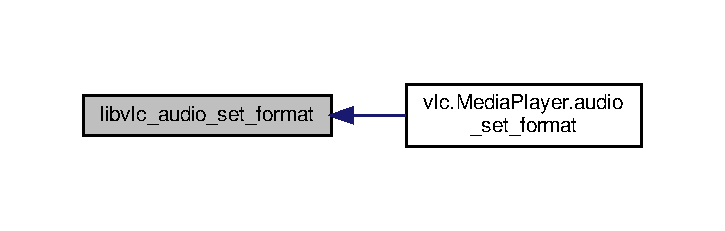
\includegraphics[width=348pt]{namespacevlc_ab91a179094998e8bf3c5be9ab109e206_icgraph}
\end{center}
\end{figure}
\mbox{\Hypertarget{namespacevlc_a0191b731e6860891d7788976a24c73b9}\label{namespacevlc_a0191b731e6860891d7788976a24c73b9}} 
\index{vlc@{vlc}!libvlc\+\_\+audio\+\_\+set\+\_\+format\+\_\+callbacks@{libvlc\+\_\+audio\+\_\+set\+\_\+format\+\_\+callbacks}}
\index{libvlc\+\_\+audio\+\_\+set\+\_\+format\+\_\+callbacks@{libvlc\+\_\+audio\+\_\+set\+\_\+format\+\_\+callbacks}!vlc@{vlc}}
\subsubsection{\texorpdfstring{libvlc\+\_\+audio\+\_\+set\+\_\+format\+\_\+callbacks()}{libvlc\_audio\_set\_format\_callbacks()}}
{\footnotesize\ttfamily def vlc.\+libvlc\+\_\+audio\+\_\+set\+\_\+format\+\_\+callbacks (\begin{DoxyParamCaption}\item[{}]{mp,  }\item[{}]{setup,  }\item[{}]{cleanup }\end{DoxyParamCaption})}

\begin{DoxyVerb}Sets decoded audio format via callbacks.
This only works in combination with L{libvlc_audio_set_callbacks}().
@param mp: the media player.
@param setup: callback to select the audio format (cannot be None).
@param cleanup: callback to release any allocated resources (or None).
@version: LibVLC 2.0.0 or later.
\end{DoxyVerb}
 Here is the caller graph for this function\+:
\nopagebreak
\begin{figure}[H]
\begin{center}
\leavevmode
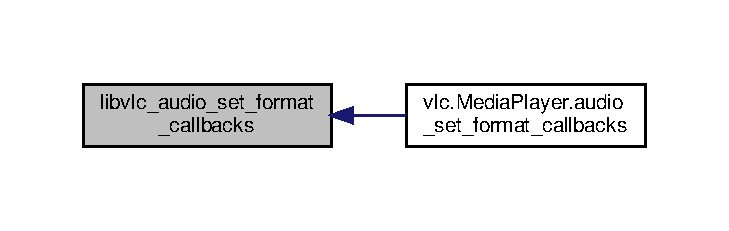
\includegraphics[width=350pt]{namespacevlc_a0191b731e6860891d7788976a24c73b9_icgraph}
\end{center}
\end{figure}
\mbox{\Hypertarget{namespacevlc_a76eac9d168adc4bab5d64c0e08e0333c}\label{namespacevlc_a76eac9d168adc4bab5d64c0e08e0333c}} 
\index{vlc@{vlc}!libvlc\+\_\+audio\+\_\+set\+\_\+mute@{libvlc\+\_\+audio\+\_\+set\+\_\+mute}}
\index{libvlc\+\_\+audio\+\_\+set\+\_\+mute@{libvlc\+\_\+audio\+\_\+set\+\_\+mute}!vlc@{vlc}}
\subsubsection{\texorpdfstring{libvlc\+\_\+audio\+\_\+set\+\_\+mute()}{libvlc\_audio\_set\_mute()}}
{\footnotesize\ttfamily def vlc.\+libvlc\+\_\+audio\+\_\+set\+\_\+mute (\begin{DoxyParamCaption}\item[{}]{p\+\_\+mi,  }\item[{}]{status }\end{DoxyParamCaption})}

\begin{DoxyVerb}Set mute status.
@param p_mi: media player.
@param status: If status is true then mute, otherwise unmute @warning This function does not always work. If there are no active audio playback stream, the mute status might not be available. If digital pass-through (S/PDIF, HDMI...) is in use, muting may be unapplicable. Also some audio output plugins do not support muting at all. @note To force silent playback, disable all audio tracks. This is more efficient and reliable than mute.
\end{DoxyVerb}
 Here is the caller graph for this function\+:
\nopagebreak
\begin{figure}[H]
\begin{center}
\leavevmode
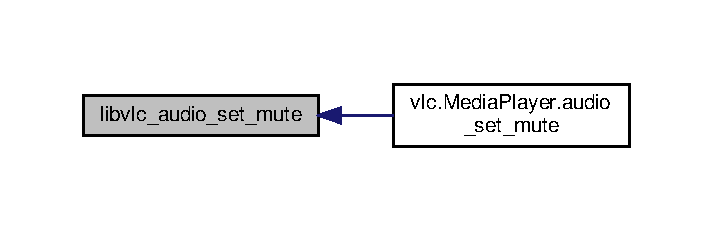
\includegraphics[width=342pt]{namespacevlc_a76eac9d168adc4bab5d64c0e08e0333c_icgraph}
\end{center}
\end{figure}
\mbox{\Hypertarget{namespacevlc_a98ac26f41a3d8271d1ec63d4a5c40289}\label{namespacevlc_a98ac26f41a3d8271d1ec63d4a5c40289}} 
\index{vlc@{vlc}!libvlc\+\_\+audio\+\_\+set\+\_\+track@{libvlc\+\_\+audio\+\_\+set\+\_\+track}}
\index{libvlc\+\_\+audio\+\_\+set\+\_\+track@{libvlc\+\_\+audio\+\_\+set\+\_\+track}!vlc@{vlc}}
\subsubsection{\texorpdfstring{libvlc\+\_\+audio\+\_\+set\+\_\+track()}{libvlc\_audio\_set\_track()}}
{\footnotesize\ttfamily def vlc.\+libvlc\+\_\+audio\+\_\+set\+\_\+track (\begin{DoxyParamCaption}\item[{}]{p\+\_\+mi,  }\item[{}]{i\+\_\+track }\end{DoxyParamCaption})}

\begin{DoxyVerb}Set current audio track.
@param p_mi: media player.
@param i_track: the track ID (i_id field from track description).
@return: 0 on success, -1 on error.
\end{DoxyVerb}
 Here is the caller graph for this function\+:
\nopagebreak
\begin{figure}[H]
\begin{center}
\leavevmode
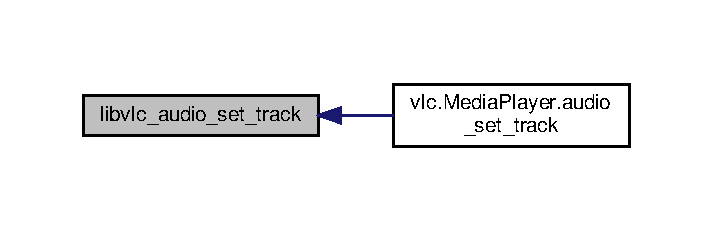
\includegraphics[width=342pt]{namespacevlc_a98ac26f41a3d8271d1ec63d4a5c40289_icgraph}
\end{center}
\end{figure}
\mbox{\Hypertarget{namespacevlc_a29afce2ad9d6cc26546b735653fe67b7}\label{namespacevlc_a29afce2ad9d6cc26546b735653fe67b7}} 
\index{vlc@{vlc}!libvlc\+\_\+audio\+\_\+set\+\_\+volume@{libvlc\+\_\+audio\+\_\+set\+\_\+volume}}
\index{libvlc\+\_\+audio\+\_\+set\+\_\+volume@{libvlc\+\_\+audio\+\_\+set\+\_\+volume}!vlc@{vlc}}
\subsubsection{\texorpdfstring{libvlc\+\_\+audio\+\_\+set\+\_\+volume()}{libvlc\_audio\_set\_volume()}}
{\footnotesize\ttfamily def vlc.\+libvlc\+\_\+audio\+\_\+set\+\_\+volume (\begin{DoxyParamCaption}\item[{}]{p\+\_\+mi,  }\item[{}]{i\+\_\+volume }\end{DoxyParamCaption})}

\begin{DoxyVerb}Set current software audio volume.
@param p_mi: media player.
@param i_volume: the volume in percents (0 = mute, 100 = 0dB).
@return: 0 if the volume was set, -1 if it was out of range.
\end{DoxyVerb}
 Here is the caller graph for this function\+:
\nopagebreak
\begin{figure}[H]
\begin{center}
\leavevmode
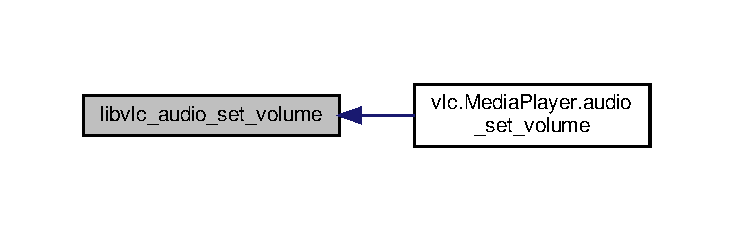
\includegraphics[width=350pt]{namespacevlc_a29afce2ad9d6cc26546b735653fe67b7_icgraph}
\end{center}
\end{figure}
\mbox{\Hypertarget{namespacevlc_a304ceaa4a56a980bf12623e54edd3444}\label{namespacevlc_a304ceaa4a56a980bf12623e54edd3444}} 
\index{vlc@{vlc}!libvlc\+\_\+audio\+\_\+set\+\_\+volume\+\_\+callback@{libvlc\+\_\+audio\+\_\+set\+\_\+volume\+\_\+callback}}
\index{libvlc\+\_\+audio\+\_\+set\+\_\+volume\+\_\+callback@{libvlc\+\_\+audio\+\_\+set\+\_\+volume\+\_\+callback}!vlc@{vlc}}
\subsubsection{\texorpdfstring{libvlc\+\_\+audio\+\_\+set\+\_\+volume\+\_\+callback()}{libvlc\_audio\_set\_volume\_callback()}}
{\footnotesize\ttfamily def vlc.\+libvlc\+\_\+audio\+\_\+set\+\_\+volume\+\_\+callback (\begin{DoxyParamCaption}\item[{}]{mp,  }\item[{}]{set\+\_\+volume }\end{DoxyParamCaption})}

\begin{DoxyVerb}Set callbacks and private data for decoded audio. This only works in
combination with L{libvlc_audio_set_callbacks}().
Use L{libvlc_audio_set_format}() or L{libvlc_audio_set_format_callbacks}()
to configure the decoded audio format.
@param mp: the media player.
@param set_volume: callback to apply audio volume, or None to apply volume in software.
@version: LibVLC 2.0.0 or later.
\end{DoxyVerb}
 Here is the caller graph for this function\+:
\nopagebreak
\begin{figure}[H]
\begin{center}
\leavevmode
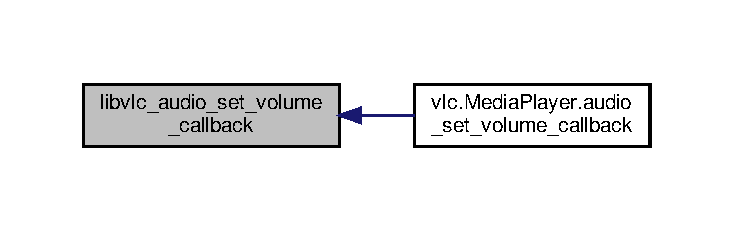
\includegraphics[width=350pt]{namespacevlc_a304ceaa4a56a980bf12623e54edd3444_icgraph}
\end{center}
\end{figure}
\mbox{\Hypertarget{namespacevlc_ad72cfaafb813c822567cc1a8fcfc8429}\label{namespacevlc_ad72cfaafb813c822567cc1a8fcfc8429}} 
\index{vlc@{vlc}!libvlc\+\_\+audio\+\_\+toggle\+\_\+mute@{libvlc\+\_\+audio\+\_\+toggle\+\_\+mute}}
\index{libvlc\+\_\+audio\+\_\+toggle\+\_\+mute@{libvlc\+\_\+audio\+\_\+toggle\+\_\+mute}!vlc@{vlc}}
\subsubsection{\texorpdfstring{libvlc\+\_\+audio\+\_\+toggle\+\_\+mute()}{libvlc\_audio\_toggle\_mute()}}
{\footnotesize\ttfamily def vlc.\+libvlc\+\_\+audio\+\_\+toggle\+\_\+mute (\begin{DoxyParamCaption}\item[{}]{p\+\_\+mi }\end{DoxyParamCaption})}

\begin{DoxyVerb}Toggle mute status.
@param p_mi: media player @warning Toggling mute atomically is not always possible: On some platforms, other processes can mute the VLC audio playback stream asynchronously. Thus, there is a small race condition where toggling will not work. See also the limitations of L{libvlc_audio_set_mute}().
\end{DoxyVerb}
 Here is the caller graph for this function\+:
\nopagebreak
\begin{figure}[H]
\begin{center}
\leavevmode
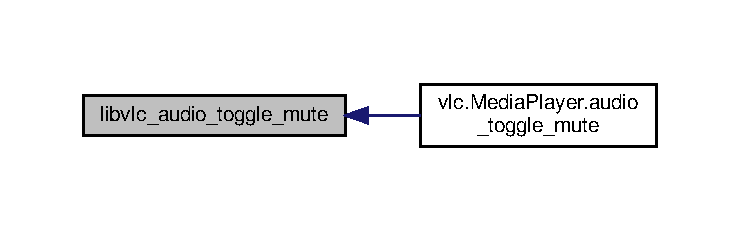
\includegraphics[width=350pt]{namespacevlc_ad72cfaafb813c822567cc1a8fcfc8429_icgraph}
\end{center}
\end{figure}
\mbox{\Hypertarget{namespacevlc_a57028e9c3f2b8ddc8722423bb560e2f7}\label{namespacevlc_a57028e9c3f2b8ddc8722423bb560e2f7}} 
\index{vlc@{vlc}!libvlc\+\_\+chapter\+\_\+descriptions\+\_\+release@{libvlc\+\_\+chapter\+\_\+descriptions\+\_\+release}}
\index{libvlc\+\_\+chapter\+\_\+descriptions\+\_\+release@{libvlc\+\_\+chapter\+\_\+descriptions\+\_\+release}!vlc@{vlc}}
\subsubsection{\texorpdfstring{libvlc\+\_\+chapter\+\_\+descriptions\+\_\+release()}{libvlc\_chapter\_descriptions\_release()}}
{\footnotesize\ttfamily def vlc.\+libvlc\+\_\+chapter\+\_\+descriptions\+\_\+release (\begin{DoxyParamCaption}\item[{}]{p\+\_\+chapters,  }\item[{}]{i\+\_\+count }\end{DoxyParamCaption})}

\begin{DoxyVerb}Release a chapter description.
@param p_chapters: chapter description array to release.
@param i_count: number of chapter descriptions to release.
@version: LibVLC 3.0.0 and later.
\end{DoxyVerb}
 \mbox{\Hypertarget{namespacevlc_ae40baed0009415ac5d90fe5fce6a0c7f}\label{namespacevlc_ae40baed0009415ac5d90fe5fce6a0c7f}} 
\index{vlc@{vlc}!libvlc\+\_\+clearerr@{libvlc\+\_\+clearerr}}
\index{libvlc\+\_\+clearerr@{libvlc\+\_\+clearerr}!vlc@{vlc}}
\subsubsection{\texorpdfstring{libvlc\+\_\+clearerr()}{libvlc\_clearerr()}}
{\footnotesize\ttfamily def vlc.\+libvlc\+\_\+clearerr (\begin{DoxyParamCaption}{ }\end{DoxyParamCaption})}

\begin{DoxyVerb}Clears the LibVLC error status for the current thread. This is optional.
By default, the error status is automatically overridden when a new error
occurs, and destroyed when the thread exits.
\end{DoxyVerb}
 \mbox{\Hypertarget{namespacevlc_a87be950b9641fe8db6fdbbbf35a472ab}\label{namespacevlc_a87be950b9641fe8db6fdbbbf35a472ab}} 
\index{vlc@{vlc}!libvlc\+\_\+clock@{libvlc\+\_\+clock}}
\index{libvlc\+\_\+clock@{libvlc\+\_\+clock}!vlc@{vlc}}
\subsubsection{\texorpdfstring{libvlc\+\_\+clock()}{libvlc\_clock()}}
{\footnotesize\ttfamily def vlc.\+libvlc\+\_\+clock (\begin{DoxyParamCaption}{ }\end{DoxyParamCaption})}

\begin{DoxyVerb}Return the current time as defined by LibVLC. The unit is the microsecond.
Time increases monotonically (regardless of time zone changes and RTC
adjustements).
The origin is arbitrary but consistent across the whole system
(e.g. the system uptim, the time since the system was booted).
@note: On systems that support it, the POSIX monotonic clock is used.
\end{DoxyVerb}
 \mbox{\Hypertarget{namespacevlc_a27caf08ba5684529165692463fc5d346}\label{namespacevlc_a27caf08ba5684529165692463fc5d346}} 
\index{vlc@{vlc}!libvlc\+\_\+dialog\+\_\+dismiss@{libvlc\+\_\+dialog\+\_\+dismiss}}
\index{libvlc\+\_\+dialog\+\_\+dismiss@{libvlc\+\_\+dialog\+\_\+dismiss}!vlc@{vlc}}
\subsubsection{\texorpdfstring{libvlc\+\_\+dialog\+\_\+dismiss()}{libvlc\_dialog\_dismiss()}}
{\footnotesize\ttfamily def vlc.\+libvlc\+\_\+dialog\+\_\+dismiss (\begin{DoxyParamCaption}\item[{}]{p\+\_\+id }\end{DoxyParamCaption})}

\begin{DoxyVerb}Dismiss a dialog
After this call, p_id won't be valid anymore
See libvlc_dialog_cbs.pf_cancel.
@param p_id: id of the dialog.
@return: 0 on success, or -1 on error.
@version: LibVLC 3.0.0 and later.
\end{DoxyVerb}
 \mbox{\Hypertarget{namespacevlc_a5ea0badeed0f8c755ec3c2ba8d575120}\label{namespacevlc_a5ea0badeed0f8c755ec3c2ba8d575120}} 
\index{vlc@{vlc}!libvlc\+\_\+dialog\+\_\+get\+\_\+context@{libvlc\+\_\+dialog\+\_\+get\+\_\+context}}
\index{libvlc\+\_\+dialog\+\_\+get\+\_\+context@{libvlc\+\_\+dialog\+\_\+get\+\_\+context}!vlc@{vlc}}
\subsubsection{\texorpdfstring{libvlc\+\_\+dialog\+\_\+get\+\_\+context()}{libvlc\_dialog\_get\_context()}}
{\footnotesize\ttfamily def vlc.\+libvlc\+\_\+dialog\+\_\+get\+\_\+context (\begin{DoxyParamCaption}\item[{}]{p\+\_\+id }\end{DoxyParamCaption})}

\begin{DoxyVerb}Return the opaque pointer associated with the dialog id.
@version: LibVLC 3.0.0 and later.
\end{DoxyVerb}
 \mbox{\Hypertarget{namespacevlc_ae828437593ff045f13c2befbe418d3f4}\label{namespacevlc_ae828437593ff045f13c2befbe418d3f4}} 
\index{vlc@{vlc}!libvlc\+\_\+dialog\+\_\+post\+\_\+action@{libvlc\+\_\+dialog\+\_\+post\+\_\+action}}
\index{libvlc\+\_\+dialog\+\_\+post\+\_\+action@{libvlc\+\_\+dialog\+\_\+post\+\_\+action}!vlc@{vlc}}
\subsubsection{\texorpdfstring{libvlc\+\_\+dialog\+\_\+post\+\_\+action()}{libvlc\_dialog\_post\_action()}}
{\footnotesize\ttfamily def vlc.\+libvlc\+\_\+dialog\+\_\+post\+\_\+action (\begin{DoxyParamCaption}\item[{}]{p\+\_\+id,  }\item[{}]{i\+\_\+action }\end{DoxyParamCaption})}

\begin{DoxyVerb}Post a question answer
After this call, p_id won't be valid anymore
See libvlc_dialog_cbs.pf_display_question.
@param p_id: id of the dialog.
@param i_action: 1 for action1, 2 for action2.
@return: 0 on success, or -1 on error.
@version: LibVLC 3.0.0 and later.
\end{DoxyVerb}
 \mbox{\Hypertarget{namespacevlc_a91274ca62987d6dc96fab02187a0ab11}\label{namespacevlc_a91274ca62987d6dc96fab02187a0ab11}} 
\index{vlc@{vlc}!libvlc\+\_\+dialog\+\_\+post\+\_\+login@{libvlc\+\_\+dialog\+\_\+post\+\_\+login}}
\index{libvlc\+\_\+dialog\+\_\+post\+\_\+login@{libvlc\+\_\+dialog\+\_\+post\+\_\+login}!vlc@{vlc}}
\subsubsection{\texorpdfstring{libvlc\+\_\+dialog\+\_\+post\+\_\+login()}{libvlc\_dialog\_post\_login()}}
{\footnotesize\ttfamily def vlc.\+libvlc\+\_\+dialog\+\_\+post\+\_\+login (\begin{DoxyParamCaption}\item[{}]{p\+\_\+id,  }\item[{}]{psz\+\_\+username,  }\item[{}]{psz\+\_\+password,  }\item[{}]{b\+\_\+store }\end{DoxyParamCaption})}

\begin{DoxyVerb}Post a login answer
After this call, p_id won't be valid anymore
See libvlc_dialog_cbs.pf_display_login.
@param p_id: id of the dialog.
@param psz_username: valid and non empty string.
@param psz_password: valid string (can be empty).
@param b_store: if true, store the credentials.
@return: 0 on success, or -1 on error.
@version: LibVLC 3.0.0 and later.
\end{DoxyVerb}
 \mbox{\Hypertarget{namespacevlc_ae2518de4fc487b909f150484dbf7b457}\label{namespacevlc_ae2518de4fc487b909f150484dbf7b457}} 
\index{vlc@{vlc}!libvlc\+\_\+dialog\+\_\+set\+\_\+context@{libvlc\+\_\+dialog\+\_\+set\+\_\+context}}
\index{libvlc\+\_\+dialog\+\_\+set\+\_\+context@{libvlc\+\_\+dialog\+\_\+set\+\_\+context}!vlc@{vlc}}
\subsubsection{\texorpdfstring{libvlc\+\_\+dialog\+\_\+set\+\_\+context()}{libvlc\_dialog\_set\_context()}}
{\footnotesize\ttfamily def vlc.\+libvlc\+\_\+dialog\+\_\+set\+\_\+context (\begin{DoxyParamCaption}\item[{}]{p\+\_\+id,  }\item[{}]{p\+\_\+context }\end{DoxyParamCaption})}

\begin{DoxyVerb}Associate an opaque pointer with the dialog id.
@version: LibVLC 3.0.0 and later.
\end{DoxyVerb}
 \mbox{\Hypertarget{namespacevlc_a850485fc3bc6fa1c7a93adfd2ac93f2b}\label{namespacevlc_a850485fc3bc6fa1c7a93adfd2ac93f2b}} 
\index{vlc@{vlc}!libvlc\+\_\+event\+\_\+attach@{libvlc\+\_\+event\+\_\+attach}}
\index{libvlc\+\_\+event\+\_\+attach@{libvlc\+\_\+event\+\_\+attach}!vlc@{vlc}}
\subsubsection{\texorpdfstring{libvlc\+\_\+event\+\_\+attach()}{libvlc\_event\_attach()}}
{\footnotesize\ttfamily def vlc.\+libvlc\+\_\+event\+\_\+attach (\begin{DoxyParamCaption}\item[{}]{p\+\_\+event\+\_\+manager,  }\item[{}]{i\+\_\+event\+\_\+type,  }\item[{}]{f\+\_\+callback,  }\item[{}]{user\+\_\+data }\end{DoxyParamCaption})}

\begin{DoxyVerb}Register for an event notification.
@param p_event_manager: the event manager to which you want to attach to. Generally it is obtained by vlc_my_object_event_manager() where my_object is the object you want to listen to.
@param i_event_type: the desired event to which we want to listen.
@param f_callback: the function to call when i_event_type occurs.
@param user_data: user provided data to carry with the event.
@return: 0 on success, ENOMEM on error.
\end{DoxyVerb}
 Here is the caller graph for this function\+:
\nopagebreak
\begin{figure}[H]
\begin{center}
\leavevmode
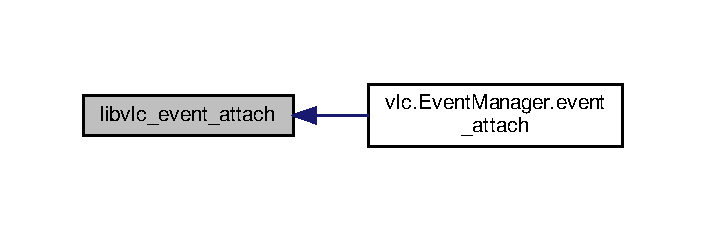
\includegraphics[width=339pt]{namespacevlc_a850485fc3bc6fa1c7a93adfd2ac93f2b_icgraph}
\end{center}
\end{figure}
\mbox{\Hypertarget{namespacevlc_a67ba99f7479ae36483024ec3e8746380}\label{namespacevlc_a67ba99f7479ae36483024ec3e8746380}} 
\index{vlc@{vlc}!libvlc\+\_\+event\+\_\+detach@{libvlc\+\_\+event\+\_\+detach}}
\index{libvlc\+\_\+event\+\_\+detach@{libvlc\+\_\+event\+\_\+detach}!vlc@{vlc}}
\subsubsection{\texorpdfstring{libvlc\+\_\+event\+\_\+detach()}{libvlc\_event\_detach()}}
{\footnotesize\ttfamily def vlc.\+libvlc\+\_\+event\+\_\+detach (\begin{DoxyParamCaption}\item[{}]{p\+\_\+event\+\_\+manager,  }\item[{}]{i\+\_\+event\+\_\+type,  }\item[{}]{f\+\_\+callback,  }\item[{}]{p\+\_\+user\+\_\+data }\end{DoxyParamCaption})}

\begin{DoxyVerb}Unregister an event notification.
@param p_event_manager: the event manager.
@param i_event_type: the desired event to which we want to unregister.
@param f_callback: the function to call when i_event_type occurs.
@param p_user_data: user provided data to carry with the event.
\end{DoxyVerb}
 Here is the caller graph for this function\+:
\nopagebreak
\begin{figure}[H]
\begin{center}
\leavevmode
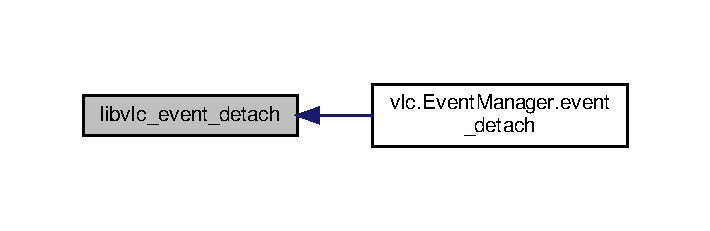
\includegraphics[width=341pt]{namespacevlc_a67ba99f7479ae36483024ec3e8746380_icgraph}
\end{center}
\end{figure}
\mbox{\Hypertarget{namespacevlc_aaec28b9045ae171b47c2212bcd8058fa}\label{namespacevlc_aaec28b9045ae171b47c2212bcd8058fa}} 
\index{vlc@{vlc}!libvlc\+\_\+event\+\_\+type\+\_\+name@{libvlc\+\_\+event\+\_\+type\+\_\+name}}
\index{libvlc\+\_\+event\+\_\+type\+\_\+name@{libvlc\+\_\+event\+\_\+type\+\_\+name}!vlc@{vlc}}
\subsubsection{\texorpdfstring{libvlc\+\_\+event\+\_\+type\+\_\+name()}{libvlc\_event\_type\_name()}}
{\footnotesize\ttfamily def vlc.\+libvlc\+\_\+event\+\_\+type\+\_\+name (\begin{DoxyParamCaption}\item[{}]{event\+\_\+type }\end{DoxyParamCaption})}

\begin{DoxyVerb}Get an event's type name.
@param event_type: the desired event.
\end{DoxyVerb}
 \mbox{\Hypertarget{namespacevlc_a517c22313b52ae70f97af003f7ef7d5a}\label{namespacevlc_a517c22313b52ae70f97af003f7ef7d5a}} 
\index{vlc@{vlc}!libvlc\+\_\+free@{libvlc\+\_\+free}}
\index{libvlc\+\_\+free@{libvlc\+\_\+free}!vlc@{vlc}}
\subsubsection{\texorpdfstring{libvlc\+\_\+free()}{libvlc\_free()}}
{\footnotesize\ttfamily def vlc.\+libvlc\+\_\+free (\begin{DoxyParamCaption}\item[{}]{ptr }\end{DoxyParamCaption})}

\begin{DoxyVerb}Frees an heap allocation returned by a LibVLC function.
If you know you're using the same underlying C run-time as the LibVLC
implementation, then you can call ANSI C free() directly instead.
@param ptr: the pointer.
\end{DoxyVerb}
 \mbox{\Hypertarget{namespacevlc_abb66509718afd388f3b587c0e28813fa}\label{namespacevlc_abb66509718afd388f3b587c0e28813fa}} 
\index{vlc@{vlc}!libvlc\+\_\+get\+\_\+changeset@{libvlc\+\_\+get\+\_\+changeset}}
\index{libvlc\+\_\+get\+\_\+changeset@{libvlc\+\_\+get\+\_\+changeset}!vlc@{vlc}}
\subsubsection{\texorpdfstring{libvlc\+\_\+get\+\_\+changeset()}{libvlc\_get\_changeset()}}
{\footnotesize\ttfamily def vlc.\+libvlc\+\_\+get\+\_\+changeset (\begin{DoxyParamCaption}{ }\end{DoxyParamCaption})}

\begin{DoxyVerb}Retrieve libvlc changeset.
Example: "aa9bce0bc4".
@return: a string containing the libvlc changeset.
\end{DoxyVerb}
 \mbox{\Hypertarget{namespacevlc_a10e241078a2da73d9ba308448d3c3192}\label{namespacevlc_a10e241078a2da73d9ba308448d3c3192}} 
\index{vlc@{vlc}!libvlc\+\_\+get\+\_\+compiler@{libvlc\+\_\+get\+\_\+compiler}}
\index{libvlc\+\_\+get\+\_\+compiler@{libvlc\+\_\+get\+\_\+compiler}!vlc@{vlc}}
\subsubsection{\texorpdfstring{libvlc\+\_\+get\+\_\+compiler()}{libvlc\_get\_compiler()}}
{\footnotesize\ttfamily def vlc.\+libvlc\+\_\+get\+\_\+compiler (\begin{DoxyParamCaption}{ }\end{DoxyParamCaption})}

\begin{DoxyVerb}Retrieve libvlc compiler version.
Example: "gcc version 4.2.3 (Ubuntu 4.2.3-2ubuntu6)".
@return: a string containing the libvlc compiler version.
\end{DoxyVerb}
 Here is the caller graph for this function\+:
\nopagebreak
\begin{figure}[H]
\begin{center}
\leavevmode
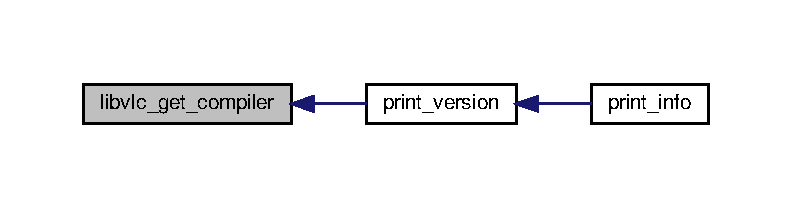
\includegraphics[width=350pt]{namespacevlc_a10e241078a2da73d9ba308448d3c3192_icgraph}
\end{center}
\end{figure}
\mbox{\Hypertarget{namespacevlc_a9533bb014114561474c90a91497dc7d6}\label{namespacevlc_a9533bb014114561474c90a91497dc7d6}} 
\index{vlc@{vlc}!libvlc\+\_\+get\+\_\+fullscreen@{libvlc\+\_\+get\+\_\+fullscreen}}
\index{libvlc\+\_\+get\+\_\+fullscreen@{libvlc\+\_\+get\+\_\+fullscreen}!vlc@{vlc}}
\subsubsection{\texorpdfstring{libvlc\+\_\+get\+\_\+fullscreen()}{libvlc\_get\_fullscreen()}}
{\footnotesize\ttfamily def vlc.\+libvlc\+\_\+get\+\_\+fullscreen (\begin{DoxyParamCaption}\item[{}]{p\+\_\+mi }\end{DoxyParamCaption})}

\begin{DoxyVerb}Get current fullscreen status.
@param p_mi: the media player.
@return: the fullscreen status (boolean) \libvlc_return_bool.
\end{DoxyVerb}
 Here is the caller graph for this function\+:
\nopagebreak
\begin{figure}[H]
\begin{center}
\leavevmode
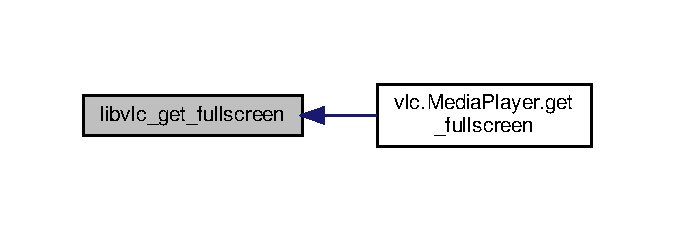
\includegraphics[width=324pt]{namespacevlc_a9533bb014114561474c90a91497dc7d6_icgraph}
\end{center}
\end{figure}
\mbox{\Hypertarget{namespacevlc_a137f63c88981266f69851dd13a25658e}\label{namespacevlc_a137f63c88981266f69851dd13a25658e}} 
\index{vlc@{vlc}!libvlc\+\_\+get\+\_\+log\+\_\+verbosity@{libvlc\+\_\+get\+\_\+log\+\_\+verbosity}}
\index{libvlc\+\_\+get\+\_\+log\+\_\+verbosity@{libvlc\+\_\+get\+\_\+log\+\_\+verbosity}!vlc@{vlc}}
\subsubsection{\texorpdfstring{libvlc\+\_\+get\+\_\+log\+\_\+verbosity()}{libvlc\_get\_log\_verbosity()}}
{\footnotesize\ttfamily def vlc.\+libvlc\+\_\+get\+\_\+log\+\_\+verbosity (\begin{DoxyParamCaption}\item[{}]{p\+\_\+instance }\end{DoxyParamCaption})}

\begin{DoxyVerb}Always returns minus one.
This function is only provided for backward compatibility.
@param p_instance: ignored.
@return: always -1.
\end{DoxyVerb}
 Here is the caller graph for this function\+:
\nopagebreak
\begin{figure}[H]
\begin{center}
\leavevmode
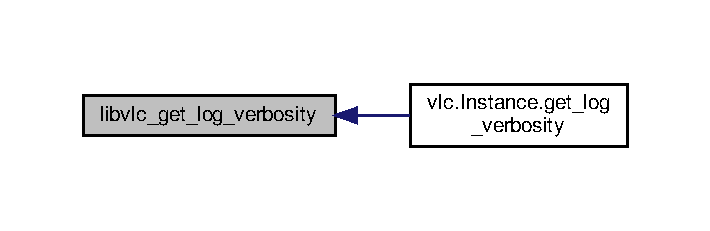
\includegraphics[width=341pt]{namespacevlc_a137f63c88981266f69851dd13a25658e_icgraph}
\end{center}
\end{figure}
\mbox{\Hypertarget{namespacevlc_abf0d92070a21456079ca64ef86649828}\label{namespacevlc_abf0d92070a21456079ca64ef86649828}} 
\index{vlc@{vlc}!libvlc\+\_\+get\+\_\+version@{libvlc\+\_\+get\+\_\+version}}
\index{libvlc\+\_\+get\+\_\+version@{libvlc\+\_\+get\+\_\+version}!vlc@{vlc}}
\subsubsection{\texorpdfstring{libvlc\+\_\+get\+\_\+version()}{libvlc\_get\_version()}}
{\footnotesize\ttfamily def vlc.\+libvlc\+\_\+get\+\_\+version (\begin{DoxyParamCaption}{ }\end{DoxyParamCaption})}

\begin{DoxyVerb}Retrieve libvlc version.
Example: "1.1.0-git The Luggage".
@return: a string containing the libvlc version.
\end{DoxyVerb}
 Here is the caller graph for this function\+:
\nopagebreak
\begin{figure}[H]
\begin{center}
\leavevmode
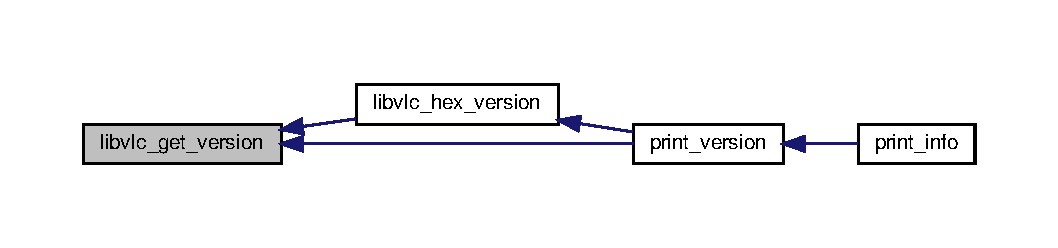
\includegraphics[width=350pt]{namespacevlc_abf0d92070a21456079ca64ef86649828_icgraph}
\end{center}
\end{figure}
\mbox{\Hypertarget{namespacevlc_a53e26e809dfb7c1f1a1f25d5e0530472}\label{namespacevlc_a53e26e809dfb7c1f1a1f25d5e0530472}} 
\index{vlc@{vlc}!libvlc\+\_\+hex\+\_\+version@{libvlc\+\_\+hex\+\_\+version}}
\index{libvlc\+\_\+hex\+\_\+version@{libvlc\+\_\+hex\+\_\+version}!vlc@{vlc}}
\subsubsection{\texorpdfstring{libvlc\+\_\+hex\+\_\+version()}{libvlc\_hex\_version()}}
{\footnotesize\ttfamily def vlc.\+libvlc\+\_\+hex\+\_\+version (\begin{DoxyParamCaption}{ }\end{DoxyParamCaption})}

\begin{DoxyVerb}Return the libvlc version in hex or 0 if unavailable.
\end{DoxyVerb}
 Here is the call graph for this function\+:
\nopagebreak
\begin{figure}[H]
\begin{center}
\leavevmode
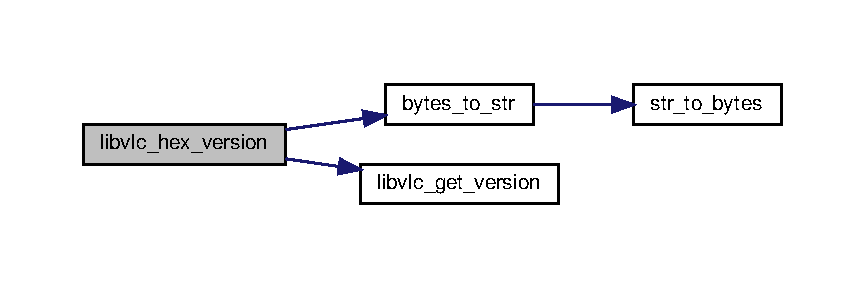
\includegraphics[width=350pt]{namespacevlc_a53e26e809dfb7c1f1a1f25d5e0530472_cgraph}
\end{center}
\end{figure}
Here is the caller graph for this function\+:
\nopagebreak
\begin{figure}[H]
\begin{center}
\leavevmode
\includegraphics[width=350pt]{namespacevlc_a53e26e809dfb7c1f1a1f25d5e0530472_icgraph}
\end{center}
\end{figure}
\mbox{\Hypertarget{namespacevlc_a1cc8217001030138b1f0ada005ce72d9}\label{namespacevlc_a1cc8217001030138b1f0ada005ce72d9}} 
\index{vlc@{vlc}!libvlc\+\_\+log\+\_\+clear@{libvlc\+\_\+log\+\_\+clear}}
\index{libvlc\+\_\+log\+\_\+clear@{libvlc\+\_\+log\+\_\+clear}!vlc@{vlc}}
\subsubsection{\texorpdfstring{libvlc\+\_\+log\+\_\+clear()}{libvlc\_log\_clear()}}
{\footnotesize\ttfamily def vlc.\+libvlc\+\_\+log\+\_\+clear (\begin{DoxyParamCaption}\item[{}]{p\+\_\+log }\end{DoxyParamCaption})}

\begin{DoxyVerb}This function does nothing.
It is only provided for backward compatibility.
@param p_log: ignored.
\end{DoxyVerb}
 \mbox{\Hypertarget{namespacevlc_a403030949bc4a5343c6a01b162395981}\label{namespacevlc_a403030949bc4a5343c6a01b162395981}} 
\index{vlc@{vlc}!libvlc\+\_\+log\+\_\+close@{libvlc\+\_\+log\+\_\+close}}
\index{libvlc\+\_\+log\+\_\+close@{libvlc\+\_\+log\+\_\+close}!vlc@{vlc}}
\subsubsection{\texorpdfstring{libvlc\+\_\+log\+\_\+close()}{libvlc\_log\_close()}}
{\footnotesize\ttfamily def vlc.\+libvlc\+\_\+log\+\_\+close (\begin{DoxyParamCaption}\item[{}]{p\+\_\+log }\end{DoxyParamCaption})}

\begin{DoxyVerb}Frees memory allocated by L{libvlc_log_open}().
@param p_log: libvlc log instance or None.
\end{DoxyVerb}
 \mbox{\Hypertarget{namespacevlc_a9743e8e0f94d5dc4855f541f9d736d7c}\label{namespacevlc_a9743e8e0f94d5dc4855f541f9d736d7c}} 
\index{vlc@{vlc}!libvlc\+\_\+log\+\_\+count@{libvlc\+\_\+log\+\_\+count}}
\index{libvlc\+\_\+log\+\_\+count@{libvlc\+\_\+log\+\_\+count}!vlc@{vlc}}
\subsubsection{\texorpdfstring{libvlc\+\_\+log\+\_\+count()}{libvlc\_log\_count()}}
{\footnotesize\ttfamily def vlc.\+libvlc\+\_\+log\+\_\+count (\begin{DoxyParamCaption}\item[{}]{p\+\_\+log }\end{DoxyParamCaption})}

\begin{DoxyVerb}Always returns zero.
This function is only provided for backward compatibility.
@param p_log: ignored.
@return: always zero.
\end{DoxyVerb}
 \mbox{\Hypertarget{namespacevlc_a9694de9d8c9b9070e0108982c90dd379}\label{namespacevlc_a9694de9d8c9b9070e0108982c90dd379}} 
\index{vlc@{vlc}!libvlc\+\_\+log\+\_\+get\+\_\+context@{libvlc\+\_\+log\+\_\+get\+\_\+context}}
\index{libvlc\+\_\+log\+\_\+get\+\_\+context@{libvlc\+\_\+log\+\_\+get\+\_\+context}!vlc@{vlc}}
\subsubsection{\texorpdfstring{libvlc\+\_\+log\+\_\+get\+\_\+context()}{libvlc\_log\_get\_context()}}
{\footnotesize\ttfamily def vlc.\+libvlc\+\_\+log\+\_\+get\+\_\+context (\begin{DoxyParamCaption}\item[{}]{ctx }\end{DoxyParamCaption})}

\begin{DoxyVerb}Gets log message debug infos.
This function retrieves self-debug information about a log message:
- the name of the VLC module emitting the message,
- the name of the source code module (i.e. file) and
- the line number within the source code module.
The returned module name and file name will be None if unknown.
The returned line number will similarly be zero if unknown.
@param ctx: message context (as passed to the @ref libvlc_log_cb callback).
@return: module module name storage (or None), file source code file name storage (or None), line source code file line number storage (or None).
@version: LibVLC 2.1.0 or later.
\end{DoxyVerb}
 \mbox{\Hypertarget{namespacevlc_acc5cfe5868875686d30894d6a631b517}\label{namespacevlc_acc5cfe5868875686d30894d6a631b517}} 
\index{vlc@{vlc}!libvlc\+\_\+log\+\_\+get\+\_\+iterator@{libvlc\+\_\+log\+\_\+get\+\_\+iterator}}
\index{libvlc\+\_\+log\+\_\+get\+\_\+iterator@{libvlc\+\_\+log\+\_\+get\+\_\+iterator}!vlc@{vlc}}
\subsubsection{\texorpdfstring{libvlc\+\_\+log\+\_\+get\+\_\+iterator()}{libvlc\_log\_get\_iterator()}}
{\footnotesize\ttfamily def vlc.\+libvlc\+\_\+log\+\_\+get\+\_\+iterator (\begin{DoxyParamCaption}\item[{}]{p\+\_\+log }\end{DoxyParamCaption})}

\begin{DoxyVerb}This function does nothing useful.
It is only provided for backward compatibility.
@param p_log: ignored.
@return: an unique pointer or None on error or if the parameter was None.
\end{DoxyVerb}
 Here is the call graph for this function\+:
\nopagebreak
\begin{figure}[H]
\begin{center}
\leavevmode
\includegraphics[width=296pt]{namespacevlc_acc5cfe5868875686d30894d6a631b517_cgraph}
\end{center}
\end{figure}
\mbox{\Hypertarget{namespacevlc_ac7af2ab7238d542708ec0da84c3d3a71}\label{namespacevlc_ac7af2ab7238d542708ec0da84c3d3a71}} 
\index{vlc@{vlc}!libvlc\+\_\+log\+\_\+get\+\_\+object@{libvlc\+\_\+log\+\_\+get\+\_\+object}}
\index{libvlc\+\_\+log\+\_\+get\+\_\+object@{libvlc\+\_\+log\+\_\+get\+\_\+object}!vlc@{vlc}}
\subsubsection{\texorpdfstring{libvlc\+\_\+log\+\_\+get\+\_\+object()}{libvlc\_log\_get\_object()}}
{\footnotesize\ttfamily def vlc.\+libvlc\+\_\+log\+\_\+get\+\_\+object (\begin{DoxyParamCaption}\item[{}]{ctx,  }\item[{}]{id }\end{DoxyParamCaption})}

\begin{DoxyVerb}Gets log message info.
This function retrieves meta-information about a log message:
- the type name of the VLC object emitting the message,
- the object header if any, and
- a temporaly-unique object identifier.
This information is mainly meant for B{manual} troubleshooting.
The returned type name may be "generic" if unknown, but it cannot be None.
The returned header will be None if unset; in current versions, the header
is used to distinguish for VLM inputs.
The returned object ID will be zero if the message is not associated with
any VLC object.
@param ctx: message context (as passed to the @ref libvlc_log_cb callback).
@return: name object name storage (or None), header object header (or None), line source code file line number storage (or None).
@version: LibVLC 2.1.0 or later.
\end{DoxyVerb}
 \mbox{\Hypertarget{namespacevlc_a37c59e68be0d4bce98e1f75b4468493b}\label{namespacevlc_a37c59e68be0d4bce98e1f75b4468493b}} 
\index{vlc@{vlc}!libvlc\+\_\+log\+\_\+iterator\+\_\+free@{libvlc\+\_\+log\+\_\+iterator\+\_\+free}}
\index{libvlc\+\_\+log\+\_\+iterator\+\_\+free@{libvlc\+\_\+log\+\_\+iterator\+\_\+free}!vlc@{vlc}}
\subsubsection{\texorpdfstring{libvlc\+\_\+log\+\_\+iterator\+\_\+free()}{libvlc\_log\_iterator\_free()}}
{\footnotesize\ttfamily def vlc.\+libvlc\+\_\+log\+\_\+iterator\+\_\+free (\begin{DoxyParamCaption}\item[{}]{p\+\_\+iter }\end{DoxyParamCaption})}

\begin{DoxyVerb}Frees memory allocated by L{libvlc_log_get_iterator}().
@param p_iter: libvlc log iterator or None.
\end{DoxyVerb}
 Here is the caller graph for this function\+:
\nopagebreak
\begin{figure}[H]
\begin{center}
\leavevmode
\includegraphics[width=328pt]{namespacevlc_a37c59e68be0d4bce98e1f75b4468493b_icgraph}
\end{center}
\end{figure}
\mbox{\Hypertarget{namespacevlc_a7637cd4511fa87f32eeff4bbfa44907b}\label{namespacevlc_a7637cd4511fa87f32eeff4bbfa44907b}} 
\index{vlc@{vlc}!libvlc\+\_\+log\+\_\+iterator\+\_\+has\+\_\+next@{libvlc\+\_\+log\+\_\+iterator\+\_\+has\+\_\+next}}
\index{libvlc\+\_\+log\+\_\+iterator\+\_\+has\+\_\+next@{libvlc\+\_\+log\+\_\+iterator\+\_\+has\+\_\+next}!vlc@{vlc}}
\subsubsection{\texorpdfstring{libvlc\+\_\+log\+\_\+iterator\+\_\+has\+\_\+next()}{libvlc\_log\_iterator\_has\_next()}}
{\footnotesize\ttfamily def vlc.\+libvlc\+\_\+log\+\_\+iterator\+\_\+has\+\_\+next (\begin{DoxyParamCaption}\item[{}]{p\+\_\+iter }\end{DoxyParamCaption})}

\begin{DoxyVerb}Always returns zero.
This function is only provided for backward compatibility.
@param p_iter: ignored.
@return: always zero.
\end{DoxyVerb}
 Here is the caller graph for this function\+:
\nopagebreak
\begin{figure}[H]
\begin{center}
\leavevmode
\includegraphics[width=350pt]{namespacevlc_a7637cd4511fa87f32eeff4bbfa44907b_icgraph}
\end{center}
\end{figure}
\mbox{\Hypertarget{namespacevlc_ae704638f284c91d4cb97d6731606dbef}\label{namespacevlc_ae704638f284c91d4cb97d6731606dbef}} 
\index{vlc@{vlc}!libvlc\+\_\+log\+\_\+iterator\+\_\+next@{libvlc\+\_\+log\+\_\+iterator\+\_\+next}}
\index{libvlc\+\_\+log\+\_\+iterator\+\_\+next@{libvlc\+\_\+log\+\_\+iterator\+\_\+next}!vlc@{vlc}}
\subsubsection{\texorpdfstring{libvlc\+\_\+log\+\_\+iterator\+\_\+next()}{libvlc\_log\_iterator\_next()}}
{\footnotesize\ttfamily def vlc.\+libvlc\+\_\+log\+\_\+iterator\+\_\+next (\begin{DoxyParamCaption}\item[{}]{p\+\_\+iter,  }\item[{}]{p\+\_\+buf }\end{DoxyParamCaption})}

\begin{DoxyVerb}Always returns None.
This function is only provided for backward compatibility.
@param p_iter: libvlc log iterator or None.
@param p_buf: ignored.
@return: always None.
\end{DoxyVerb}
 Here is the caller graph for this function\+:
\nopagebreak
\begin{figure}[H]
\begin{center}
\leavevmode
\includegraphics[width=350pt]{namespacevlc_ae704638f284c91d4cb97d6731606dbef_icgraph}
\end{center}
\end{figure}
\mbox{\Hypertarget{namespacevlc_a03e79554e536d7e5cb215042e619966e}\label{namespacevlc_a03e79554e536d7e5cb215042e619966e}} 
\index{vlc@{vlc}!libvlc\+\_\+log\+\_\+open@{libvlc\+\_\+log\+\_\+open}}
\index{libvlc\+\_\+log\+\_\+open@{libvlc\+\_\+log\+\_\+open}!vlc@{vlc}}
\subsubsection{\texorpdfstring{libvlc\+\_\+log\+\_\+open()}{libvlc\_log\_open()}}
{\footnotesize\ttfamily def vlc.\+libvlc\+\_\+log\+\_\+open (\begin{DoxyParamCaption}\item[{}]{p\+\_\+instance }\end{DoxyParamCaption})}

\begin{DoxyVerb}This function does nothing useful.
It is only provided for backward compatibility.
@param p_instance: libvlc instance.
@return: an unique pointer or None on error.
\end{DoxyVerb}
 Here is the caller graph for this function\+:
\nopagebreak
\begin{figure}[H]
\begin{center}
\leavevmode
\includegraphics[width=311pt]{namespacevlc_a03e79554e536d7e5cb215042e619966e_icgraph}
\end{center}
\end{figure}
\mbox{\Hypertarget{namespacevlc_aff40c0e783a0949925936432b4beba34}\label{namespacevlc_aff40c0e783a0949925936432b4beba34}} 
\index{vlc@{vlc}!libvlc\+\_\+log\+\_\+set@{libvlc\+\_\+log\+\_\+set}}
\index{libvlc\+\_\+log\+\_\+set@{libvlc\+\_\+log\+\_\+set}!vlc@{vlc}}
\subsubsection{\texorpdfstring{libvlc\+\_\+log\+\_\+set()}{libvlc\_log\_set()}}
{\footnotesize\ttfamily def vlc.\+libvlc\+\_\+log\+\_\+set (\begin{DoxyParamCaption}\item[{}]{p\+\_\+instance,  }\item[{}]{cb,  }\item[{}]{data }\end{DoxyParamCaption})}

\begin{DoxyVerb}Sets the logging callback for a LibVLC instance.
This function is thread-safe: it will wait for any pending callbacks
invocation to complete.
@param cb: callback function pointer.
@param data: opaque data pointer for the callback function @note Some log messages (especially debug) are emitted by LibVLC while is being initialized. These messages cannot be captured with this interface. @warning A deadlock may occur if this function is called from the callback.
@param p_instance: libvlc instance.
@version: LibVLC 2.1.0 or later.
\end{DoxyVerb}
 Here is the caller graph for this function\+:
\nopagebreak
\begin{figure}[H]
\begin{center}
\leavevmode
\includegraphics[width=296pt]{namespacevlc_aff40c0e783a0949925936432b4beba34_icgraph}
\end{center}
\end{figure}
\mbox{\Hypertarget{namespacevlc_aa18225aa223a1abfd7245a682fd599a0}\label{namespacevlc_aa18225aa223a1abfd7245a682fd599a0}} 
\index{vlc@{vlc}!libvlc\+\_\+log\+\_\+set\+\_\+file@{libvlc\+\_\+log\+\_\+set\+\_\+file}}
\index{libvlc\+\_\+log\+\_\+set\+\_\+file@{libvlc\+\_\+log\+\_\+set\+\_\+file}!vlc@{vlc}}
\subsubsection{\texorpdfstring{libvlc\+\_\+log\+\_\+set\+\_\+file()}{libvlc\_log\_set\_file()}}
{\footnotesize\ttfamily def vlc.\+libvlc\+\_\+log\+\_\+set\+\_\+file (\begin{DoxyParamCaption}\item[{}]{p\+\_\+instance,  }\item[{}]{stream }\end{DoxyParamCaption})}

\begin{DoxyVerb}Sets up logging to a file.
@param p_instance: libvlc instance.
@param stream: FILE pointer opened for writing (the FILE pointer must remain valid until L{libvlc_log_unset}()).
@version: LibVLC 2.1.0 or later.
\end{DoxyVerb}
 Here is the caller graph for this function\+:
\nopagebreak
\begin{figure}[H]
\begin{center}
\leavevmode
\includegraphics[width=332pt]{namespacevlc_aa18225aa223a1abfd7245a682fd599a0_icgraph}
\end{center}
\end{figure}
\mbox{\Hypertarget{namespacevlc_ab8183b479ddf3d672f4044a9a3805b06}\label{namespacevlc_ab8183b479ddf3d672f4044a9a3805b06}} 
\index{vlc@{vlc}!libvlc\+\_\+log\+\_\+unset@{libvlc\+\_\+log\+\_\+unset}}
\index{libvlc\+\_\+log\+\_\+unset@{libvlc\+\_\+log\+\_\+unset}!vlc@{vlc}}
\subsubsection{\texorpdfstring{libvlc\+\_\+log\+\_\+unset()}{libvlc\_log\_unset()}}
{\footnotesize\ttfamily def vlc.\+libvlc\+\_\+log\+\_\+unset (\begin{DoxyParamCaption}\item[{}]{p\+\_\+instance }\end{DoxyParamCaption})}

\begin{DoxyVerb}Unsets the logging callback.
This function deregisters the logging callback for a LibVLC instance.
This is rarely needed as the callback is implicitly unset when the instance
is destroyed.
@note: This function will wait for any pending callbacks invocation to
complete (causing a deadlock if called from within the callback).
@param p_instance: libvlc instance.
@version: LibVLC 2.1.0 or later.
\end{DoxyVerb}
 Here is the caller graph for this function\+:
\nopagebreak
\begin{figure}[H]
\begin{center}
\leavevmode
\includegraphics[width=317pt]{namespacevlc_ab8183b479ddf3d672f4044a9a3805b06_icgraph}
\end{center}
\end{figure}
\mbox{\Hypertarget{namespacevlc_adbf254196790831139b165b8f20bab19}\label{namespacevlc_adbf254196790831139b165b8f20bab19}} 
\index{vlc@{vlc}!libvlc\+\_\+media\+\_\+add\+\_\+option@{libvlc\+\_\+media\+\_\+add\+\_\+option}}
\index{libvlc\+\_\+media\+\_\+add\+\_\+option@{libvlc\+\_\+media\+\_\+add\+\_\+option}!vlc@{vlc}}
\subsubsection{\texorpdfstring{libvlc\+\_\+media\+\_\+add\+\_\+option()}{libvlc\_media\_add\_option()}}
{\footnotesize\ttfamily def vlc.\+libvlc\+\_\+media\+\_\+add\+\_\+option (\begin{DoxyParamCaption}\item[{}]{p\+\_\+md,  }\item[{}]{psz\+\_\+options }\end{DoxyParamCaption})}

\begin{DoxyVerb}Add an option to the media.
This option will be used to determine how the media_player will
read the media. This allows to use VLC's advanced
reading/streaming options on a per-media basis.
@note: The options are listed in 'vlc --long-help' from the command line,
e.g. "-sout-all". Keep in mind that available options and their semantics
vary across LibVLC versions and builds.
@warning: Not all options affects L{Media} objects:
Specifically, due to architectural issues most audio and video options,
such as text renderer options, have no effects on an individual media.
These options must be set through L{libvlc_new}() instead.
@param p_md: the media descriptor.
@param psz_options: the options (as a string).
\end{DoxyVerb}
 Here is the caller graph for this function\+:
\nopagebreak
\begin{figure}[H]
\begin{center}
\leavevmode
\includegraphics[width=350pt]{namespacevlc_adbf254196790831139b165b8f20bab19_icgraph}
\end{center}
\end{figure}
\mbox{\Hypertarget{namespacevlc_a7dc1f3fd16f555dec3a3bf5466c86d5f}\label{namespacevlc_a7dc1f3fd16f555dec3a3bf5466c86d5f}} 
\index{vlc@{vlc}!libvlc\+\_\+media\+\_\+add\+\_\+option\+\_\+flag@{libvlc\+\_\+media\+\_\+add\+\_\+option\+\_\+flag}}
\index{libvlc\+\_\+media\+\_\+add\+\_\+option\+\_\+flag@{libvlc\+\_\+media\+\_\+add\+\_\+option\+\_\+flag}!vlc@{vlc}}
\subsubsection{\texorpdfstring{libvlc\+\_\+media\+\_\+add\+\_\+option\+\_\+flag()}{libvlc\_media\_add\_option\_flag()}}
{\footnotesize\ttfamily def vlc.\+libvlc\+\_\+media\+\_\+add\+\_\+option\+\_\+flag (\begin{DoxyParamCaption}\item[{}]{p\+\_\+md,  }\item[{}]{psz\+\_\+options,  }\item[{}]{i\+\_\+flags }\end{DoxyParamCaption})}

\begin{DoxyVerb}Add an option to the media with configurable flags.
This option will be used to determine how the media_player will
read the media. This allows to use VLC's advanced
reading/streaming options on a per-media basis.
The options are detailed in vlc --long-help, for instance
"--sout-all". Note that all options are not usable on medias:
specifically, due to architectural issues, video-related options
such as text renderer options cannot be set on a single media. They
must be set on the whole libvlc instance instead.
@param p_md: the media descriptor.
@param psz_options: the options (as a string).
@param i_flags: the flags for this option.
\end{DoxyVerb}
 Here is the caller graph for this function\+:
\nopagebreak
\begin{figure}[H]
\begin{center}
\leavevmode
\includegraphics[width=350pt]{namespacevlc_a7dc1f3fd16f555dec3a3bf5466c86d5f_icgraph}
\end{center}
\end{figure}
\mbox{\Hypertarget{namespacevlc_ae17b8e9a27594920a38298179a0198e6}\label{namespacevlc_ae17b8e9a27594920a38298179a0198e6}} 
\index{vlc@{vlc}!libvlc\+\_\+media\+\_\+discoverer\+\_\+event\+\_\+manager@{libvlc\+\_\+media\+\_\+discoverer\+\_\+event\+\_\+manager}}
\index{libvlc\+\_\+media\+\_\+discoverer\+\_\+event\+\_\+manager@{libvlc\+\_\+media\+\_\+discoverer\+\_\+event\+\_\+manager}!vlc@{vlc}}
\subsubsection{\texorpdfstring{libvlc\+\_\+media\+\_\+discoverer\+\_\+event\+\_\+manager()}{libvlc\_media\_discoverer\_event\_manager()}}
{\footnotesize\ttfamily def vlc.\+libvlc\+\_\+media\+\_\+discoverer\+\_\+event\+\_\+manager (\begin{DoxyParamCaption}\item[{}]{p\+\_\+mdis }\end{DoxyParamCaption})}

\begin{DoxyVerb}Get event manager from media service discover object.
\deprecated Useless, media_discoverer events are only triggered when calling
L{libvlc_media_discoverer_start}() and L{libvlc_media_discoverer_stop}().
@param p_mdis: media service discover object.
@return: event manager object.
\end{DoxyVerb}
 Here is the call graph for this function\+:
\nopagebreak
\begin{figure}[H]
\begin{center}
\leavevmode
\includegraphics[width=306pt]{namespacevlc_ae17b8e9a27594920a38298179a0198e6_cgraph}
\end{center}
\end{figure}
Here is the caller graph for this function\+:
\nopagebreak
\begin{figure}[H]
\begin{center}
\leavevmode
\includegraphics[width=350pt]{namespacevlc_ae17b8e9a27594920a38298179a0198e6_icgraph}
\end{center}
\end{figure}
\mbox{\Hypertarget{namespacevlc_a67f645168455fbbbb9199ff602583113}\label{namespacevlc_a67f645168455fbbbb9199ff602583113}} 
\index{vlc@{vlc}!libvlc\+\_\+media\+\_\+discoverer\+\_\+is\+\_\+running@{libvlc\+\_\+media\+\_\+discoverer\+\_\+is\+\_\+running}}
\index{libvlc\+\_\+media\+\_\+discoverer\+\_\+is\+\_\+running@{libvlc\+\_\+media\+\_\+discoverer\+\_\+is\+\_\+running}!vlc@{vlc}}
\subsubsection{\texorpdfstring{libvlc\+\_\+media\+\_\+discoverer\+\_\+is\+\_\+running()}{libvlc\_media\_discoverer\_is\_running()}}
{\footnotesize\ttfamily def vlc.\+libvlc\+\_\+media\+\_\+discoverer\+\_\+is\+\_\+running (\begin{DoxyParamCaption}\item[{}]{p\+\_\+mdis }\end{DoxyParamCaption})}

\begin{DoxyVerb}Query if media service discover object is running.
@param p_mdis: media service discover object.
@return: true if running, false if not \libvlc_return_bool.
\end{DoxyVerb}
 Here is the caller graph for this function\+:
\nopagebreak
\begin{figure}[H]
\begin{center}
\leavevmode
\includegraphics[width=350pt]{namespacevlc_a67f645168455fbbbb9199ff602583113_icgraph}
\end{center}
\end{figure}
\mbox{\Hypertarget{namespacevlc_ad4eb84abb29b0c9c742ce5444bb21d69}\label{namespacevlc_ad4eb84abb29b0c9c742ce5444bb21d69}} 
\index{vlc@{vlc}!libvlc\+\_\+media\+\_\+discoverer\+\_\+list\+\_\+get@{libvlc\+\_\+media\+\_\+discoverer\+\_\+list\+\_\+get}}
\index{libvlc\+\_\+media\+\_\+discoverer\+\_\+list\+\_\+get@{libvlc\+\_\+media\+\_\+discoverer\+\_\+list\+\_\+get}!vlc@{vlc}}
\subsubsection{\texorpdfstring{libvlc\+\_\+media\+\_\+discoverer\+\_\+list\+\_\+get()}{libvlc\_media\_discoverer\_list\_get()}}
{\footnotesize\ttfamily def vlc.\+libvlc\+\_\+media\+\_\+discoverer\+\_\+list\+\_\+get (\begin{DoxyParamCaption}\item[{}]{p\+\_\+inst,  }\item[{}]{i\+\_\+cat,  }\item[{}]{ppp\+\_\+services }\end{DoxyParamCaption})}

\begin{DoxyVerb}Get media discoverer services by category.
@param p_inst: libvlc instance.
@param i_cat: category of services to fetch.
@param ppp_services: address to store an allocated array of media discoverer services (must be freed with L{libvlc_media_discoverer_list_release}() by the caller) [OUT].
@return: the number of media discoverer services (0 on error).
@version: LibVLC 3.0.0 and later.
\end{DoxyVerb}
 Here is the caller graph for this function\+:
\nopagebreak
\begin{figure}[H]
\begin{center}
\leavevmode
\includegraphics[width=341pt]{namespacevlc_ad4eb84abb29b0c9c742ce5444bb21d69_icgraph}
\end{center}
\end{figure}
\mbox{\Hypertarget{namespacevlc_a0b232d83e1c5d5876f6438665a63532f}\label{namespacevlc_a0b232d83e1c5d5876f6438665a63532f}} 
\index{vlc@{vlc}!libvlc\+\_\+media\+\_\+discoverer\+\_\+list\+\_\+release@{libvlc\+\_\+media\+\_\+discoverer\+\_\+list\+\_\+release}}
\index{libvlc\+\_\+media\+\_\+discoverer\+\_\+list\+\_\+release@{libvlc\+\_\+media\+\_\+discoverer\+\_\+list\+\_\+release}!vlc@{vlc}}
\subsubsection{\texorpdfstring{libvlc\+\_\+media\+\_\+discoverer\+\_\+list\+\_\+release()}{libvlc\_media\_discoverer\_list\_release()}}
{\footnotesize\ttfamily def vlc.\+libvlc\+\_\+media\+\_\+discoverer\+\_\+list\+\_\+release (\begin{DoxyParamCaption}\item[{}]{pp\+\_\+services,  }\item[{}]{i\+\_\+count }\end{DoxyParamCaption})}

\begin{DoxyVerb}Release an array of media discoverer services.
@param pp_services: array to release.
@param i_count: number of elements in the array.
@version: LibVLC 3.0.0 and later. See L{libvlc_media_discoverer_list_get}().
\end{DoxyVerb}
 \mbox{\Hypertarget{namespacevlc_a3b2a41bfb1a505c80af56dad8ce507ac}\label{namespacevlc_a3b2a41bfb1a505c80af56dad8ce507ac}} 
\index{vlc@{vlc}!libvlc\+\_\+media\+\_\+discoverer\+\_\+localized\+\_\+name@{libvlc\+\_\+media\+\_\+discoverer\+\_\+localized\+\_\+name}}
\index{libvlc\+\_\+media\+\_\+discoverer\+\_\+localized\+\_\+name@{libvlc\+\_\+media\+\_\+discoverer\+\_\+localized\+\_\+name}!vlc@{vlc}}
\subsubsection{\texorpdfstring{libvlc\+\_\+media\+\_\+discoverer\+\_\+localized\+\_\+name()}{libvlc\_media\_discoverer\_localized\_name()}}
{\footnotesize\ttfamily def vlc.\+libvlc\+\_\+media\+\_\+discoverer\+\_\+localized\+\_\+name (\begin{DoxyParamCaption}\item[{}]{p\+\_\+mdis }\end{DoxyParamCaption})}

\begin{DoxyVerb}Get media service discover object its localized name.
\deprecated Useless, use L{libvlc_media_discoverer_list_get}() to get the
longname of the service discovery.
@param p_mdis: media discover object.
@return: localized name or None if the media_discoverer is not started.
\end{DoxyVerb}
 Here is the caller graph for this function\+:
\nopagebreak
\begin{figure}[H]
\begin{center}
\leavevmode
\includegraphics[width=350pt]{namespacevlc_a3b2a41bfb1a505c80af56dad8ce507ac_icgraph}
\end{center}
\end{figure}
\mbox{\Hypertarget{namespacevlc_a7a67121178840567c764d45a7965d52b}\label{namespacevlc_a7a67121178840567c764d45a7965d52b}} 
\index{vlc@{vlc}!libvlc\+\_\+media\+\_\+discoverer\+\_\+media\+\_\+list@{libvlc\+\_\+media\+\_\+discoverer\+\_\+media\+\_\+list}}
\index{libvlc\+\_\+media\+\_\+discoverer\+\_\+media\+\_\+list@{libvlc\+\_\+media\+\_\+discoverer\+\_\+media\+\_\+list}!vlc@{vlc}}
\subsubsection{\texorpdfstring{libvlc\+\_\+media\+\_\+discoverer\+\_\+media\+\_\+list()}{libvlc\_media\_discoverer\_media\_list()}}
{\footnotesize\ttfamily def vlc.\+libvlc\+\_\+media\+\_\+discoverer\+\_\+media\+\_\+list (\begin{DoxyParamCaption}\item[{}]{p\+\_\+mdis }\end{DoxyParamCaption})}

\begin{DoxyVerb}Get media service discover media list.
@param p_mdis: media service discover object.
@return: list of media items.
\end{DoxyVerb}
 Here is the call graph for this function\+:
\nopagebreak
\begin{figure}[H]
\begin{center}
\leavevmode
\includegraphics[width=306pt]{namespacevlc_a7a67121178840567c764d45a7965d52b_cgraph}
\end{center}
\end{figure}
Here is the caller graph for this function\+:
\nopagebreak
\begin{figure}[H]
\begin{center}
\leavevmode
\includegraphics[width=350pt]{namespacevlc_a7a67121178840567c764d45a7965d52b_icgraph}
\end{center}
\end{figure}
\mbox{\Hypertarget{namespacevlc_aca3af54c1b5d61bc7877d189b8fda18b}\label{namespacevlc_aca3af54c1b5d61bc7877d189b8fda18b}} 
\index{vlc@{vlc}!libvlc\+\_\+media\+\_\+discoverer\+\_\+new@{libvlc\+\_\+media\+\_\+discoverer\+\_\+new}}
\index{libvlc\+\_\+media\+\_\+discoverer\+\_\+new@{libvlc\+\_\+media\+\_\+discoverer\+\_\+new}!vlc@{vlc}}
\subsubsection{\texorpdfstring{libvlc\+\_\+media\+\_\+discoverer\+\_\+new()}{libvlc\_media\_discoverer\_new()}}
{\footnotesize\ttfamily def vlc.\+libvlc\+\_\+media\+\_\+discoverer\+\_\+new (\begin{DoxyParamCaption}\item[{}]{p\+\_\+inst,  }\item[{}]{psz\+\_\+name }\end{DoxyParamCaption})}

\begin{DoxyVerb}Create a media discoverer object by name.
After this object is created, you should attach to media_list events in
order to be notified of new items discovered.
You need to call L{libvlc_media_discoverer_start}() in order to start the
discovery.
See L{libvlc_media_discoverer_media_list}
See L{libvlc_media_discoverer_event_manager}
See L{libvlc_media_discoverer_start}.
@param p_inst: libvlc instance.
@param psz_name: service name; use L{libvlc_media_discoverer_list_get}() to get a list of the discoverer names available in this libVLC instance.
@return: media discover object or None in case of error.
@version: LibVLC 3.0.0 or later.
\end{DoxyVerb}
 Here is the call graph for this function\+:
\nopagebreak
\begin{figure}[H]
\begin{center}
\leavevmode
\includegraphics[width=329pt]{namespacevlc_aca3af54c1b5d61bc7877d189b8fda18b_cgraph}
\end{center}
\end{figure}
Here is the caller graph for this function\+:
\nopagebreak
\begin{figure}[H]
\begin{center}
\leavevmode
\includegraphics[width=350pt]{namespacevlc_aca3af54c1b5d61bc7877d189b8fda18b_icgraph}
\end{center}
\end{figure}
\mbox{\Hypertarget{namespacevlc_a767b87c1a19544f94b98794de5728cde}\label{namespacevlc_a767b87c1a19544f94b98794de5728cde}} 
\index{vlc@{vlc}!libvlc\+\_\+media\+\_\+discoverer\+\_\+new\+\_\+from\+\_\+name@{libvlc\+\_\+media\+\_\+discoverer\+\_\+new\+\_\+from\+\_\+name}}
\index{libvlc\+\_\+media\+\_\+discoverer\+\_\+new\+\_\+from\+\_\+name@{libvlc\+\_\+media\+\_\+discoverer\+\_\+new\+\_\+from\+\_\+name}!vlc@{vlc}}
\subsubsection{\texorpdfstring{libvlc\+\_\+media\+\_\+discoverer\+\_\+new\+\_\+from\+\_\+name()}{libvlc\_media\_discoverer\_new\_from\_name()}}
{\footnotesize\ttfamily def vlc.\+libvlc\+\_\+media\+\_\+discoverer\+\_\+new\+\_\+from\+\_\+name (\begin{DoxyParamCaption}\item[{}]{p\+\_\+inst,  }\item[{}]{psz\+\_\+name }\end{DoxyParamCaption})}

\begin{DoxyVerb}\deprecated Use L{libvlc_media_discoverer_new}() and L{libvlc_media_discoverer_start}().
\end{DoxyVerb}
 Here is the call graph for this function\+:
\nopagebreak
\begin{figure}[H]
\begin{center}
\leavevmode
\includegraphics[width=306pt]{namespacevlc_a767b87c1a19544f94b98794de5728cde_cgraph}
\end{center}
\end{figure}
Here is the caller graph for this function\+:
\nopagebreak
\begin{figure}[H]
\begin{center}
\leavevmode
\includegraphics[width=350pt]{namespacevlc_a767b87c1a19544f94b98794de5728cde_icgraph}
\end{center}
\end{figure}
\mbox{\Hypertarget{namespacevlc_adddb8a8785beb08b0599ccb43c3ddffd}\label{namespacevlc_adddb8a8785beb08b0599ccb43c3ddffd}} 
\index{vlc@{vlc}!libvlc\+\_\+media\+\_\+discoverer\+\_\+release@{libvlc\+\_\+media\+\_\+discoverer\+\_\+release}}
\index{libvlc\+\_\+media\+\_\+discoverer\+\_\+release@{libvlc\+\_\+media\+\_\+discoverer\+\_\+release}!vlc@{vlc}}
\subsubsection{\texorpdfstring{libvlc\+\_\+media\+\_\+discoverer\+\_\+release()}{libvlc\_media\_discoverer\_release()}}
{\footnotesize\ttfamily def vlc.\+libvlc\+\_\+media\+\_\+discoverer\+\_\+release (\begin{DoxyParamCaption}\item[{}]{p\+\_\+mdis }\end{DoxyParamCaption})}

\begin{DoxyVerb}Release media discover object. If the reference count reaches 0, then
the object will be released.
@param p_mdis: media service discover object.
\end{DoxyVerb}
 Here is the caller graph for this function\+:
\nopagebreak
\begin{figure}[H]
\begin{center}
\leavevmode
\includegraphics[width=350pt]{namespacevlc_adddb8a8785beb08b0599ccb43c3ddffd_icgraph}
\end{center}
\end{figure}
\mbox{\Hypertarget{namespacevlc_a717cf33da5cb426ea198e5cc7c23fcac}\label{namespacevlc_a717cf33da5cb426ea198e5cc7c23fcac}} 
\index{vlc@{vlc}!libvlc\+\_\+media\+\_\+discoverer\+\_\+start@{libvlc\+\_\+media\+\_\+discoverer\+\_\+start}}
\index{libvlc\+\_\+media\+\_\+discoverer\+\_\+start@{libvlc\+\_\+media\+\_\+discoverer\+\_\+start}!vlc@{vlc}}
\subsubsection{\texorpdfstring{libvlc\+\_\+media\+\_\+discoverer\+\_\+start()}{libvlc\_media\_discoverer\_start()}}
{\footnotesize\ttfamily def vlc.\+libvlc\+\_\+media\+\_\+discoverer\+\_\+start (\begin{DoxyParamCaption}\item[{}]{p\+\_\+mdis }\end{DoxyParamCaption})}

\begin{DoxyVerb}Start media discovery.
To stop it, call L{libvlc_media_discoverer_stop}() or
L{libvlc_media_discoverer_list_release}() directly.
See L{libvlc_media_discoverer_stop}.
@param p_mdis: media discover object.
@return: -1 in case of error, 0 otherwise.
@version: LibVLC 3.0.0 or later.
\end{DoxyVerb}
 Here is the caller graph for this function\+:
\nopagebreak
\begin{figure}[H]
\begin{center}
\leavevmode
\includegraphics[width=350pt]{namespacevlc_a717cf33da5cb426ea198e5cc7c23fcac_icgraph}
\end{center}
\end{figure}
\mbox{\Hypertarget{namespacevlc_a90f5d66c443b544188e64f67dc85e95a}\label{namespacevlc_a90f5d66c443b544188e64f67dc85e95a}} 
\index{vlc@{vlc}!libvlc\+\_\+media\+\_\+discoverer\+\_\+stop@{libvlc\+\_\+media\+\_\+discoverer\+\_\+stop}}
\index{libvlc\+\_\+media\+\_\+discoverer\+\_\+stop@{libvlc\+\_\+media\+\_\+discoverer\+\_\+stop}!vlc@{vlc}}
\subsubsection{\texorpdfstring{libvlc\+\_\+media\+\_\+discoverer\+\_\+stop()}{libvlc\_media\_discoverer\_stop()}}
{\footnotesize\ttfamily def vlc.\+libvlc\+\_\+media\+\_\+discoverer\+\_\+stop (\begin{DoxyParamCaption}\item[{}]{p\+\_\+mdis }\end{DoxyParamCaption})}

\begin{DoxyVerb}Stop media discovery.
See L{libvlc_media_discoverer_start}.
@param p_mdis: media discover object.
@version: LibVLC 3.0.0 or later.
\end{DoxyVerb}
 Here is the caller graph for this function\+:
\nopagebreak
\begin{figure}[H]
\begin{center}
\leavevmode
\includegraphics[width=350pt]{namespacevlc_a90f5d66c443b544188e64f67dc85e95a_icgraph}
\end{center}
\end{figure}
\mbox{\Hypertarget{namespacevlc_a20f923172a3ea8b7f3c254e234336d7b}\label{namespacevlc_a20f923172a3ea8b7f3c254e234336d7b}} 
\index{vlc@{vlc}!libvlc\+\_\+media\+\_\+duplicate@{libvlc\+\_\+media\+\_\+duplicate}}
\index{libvlc\+\_\+media\+\_\+duplicate@{libvlc\+\_\+media\+\_\+duplicate}!vlc@{vlc}}
\subsubsection{\texorpdfstring{libvlc\+\_\+media\+\_\+duplicate()}{libvlc\_media\_duplicate()}}
{\footnotesize\ttfamily def vlc.\+libvlc\+\_\+media\+\_\+duplicate (\begin{DoxyParamCaption}\item[{}]{p\+\_\+md }\end{DoxyParamCaption})}

\begin{DoxyVerb}Duplicate a media descriptor object.
@param p_md: a media descriptor object.
\end{DoxyVerb}
 Here is the call graph for this function\+:
\nopagebreak
\begin{figure}[H]
\begin{center}
\leavevmode
\includegraphics[width=300pt]{namespacevlc_a20f923172a3ea8b7f3c254e234336d7b_cgraph}
\end{center}
\end{figure}
Here is the caller graph for this function\+:
\nopagebreak
\begin{figure}[H]
\begin{center}
\leavevmode
\includegraphics[width=332pt]{namespacevlc_a20f923172a3ea8b7f3c254e234336d7b_icgraph}
\end{center}
\end{figure}
\mbox{\Hypertarget{namespacevlc_a2b3476422efeca7d595d8371533eaa58}\label{namespacevlc_a2b3476422efeca7d595d8371533eaa58}} 
\index{vlc@{vlc}!libvlc\+\_\+media\+\_\+event\+\_\+manager@{libvlc\+\_\+media\+\_\+event\+\_\+manager}}
\index{libvlc\+\_\+media\+\_\+event\+\_\+manager@{libvlc\+\_\+media\+\_\+event\+\_\+manager}!vlc@{vlc}}
\subsubsection{\texorpdfstring{libvlc\+\_\+media\+\_\+event\+\_\+manager()}{libvlc\_media\_event\_manager()}}
{\footnotesize\ttfamily def vlc.\+libvlc\+\_\+media\+\_\+event\+\_\+manager (\begin{DoxyParamCaption}\item[{}]{p\+\_\+md }\end{DoxyParamCaption})}

\begin{DoxyVerb}Get event manager from media descriptor object.
NOTE: this function doesn't increment reference counting.
@param p_md: a media descriptor object.
@return: event manager object.
\end{DoxyVerb}
 Here is the call graph for this function\+:
\nopagebreak
\begin{figure}[H]
\begin{center}
\leavevmode
\includegraphics[width=285pt]{namespacevlc_a2b3476422efeca7d595d8371533eaa58_cgraph}
\end{center}
\end{figure}
Here is the caller graph for this function\+:
\nopagebreak
\begin{figure}[H]
\begin{center}
\leavevmode
\includegraphics[width=344pt]{namespacevlc_a2b3476422efeca7d595d8371533eaa58_icgraph}
\end{center}
\end{figure}
\mbox{\Hypertarget{namespacevlc_a9f7b1ab0dd2f4efbdd9f1d9fd8cf5fc9}\label{namespacevlc_a9f7b1ab0dd2f4efbdd9f1d9fd8cf5fc9}} 
\index{vlc@{vlc}!libvlc\+\_\+media\+\_\+get\+\_\+codec\+\_\+description@{libvlc\+\_\+media\+\_\+get\+\_\+codec\+\_\+description}}
\index{libvlc\+\_\+media\+\_\+get\+\_\+codec\+\_\+description@{libvlc\+\_\+media\+\_\+get\+\_\+codec\+\_\+description}!vlc@{vlc}}
\subsubsection{\texorpdfstring{libvlc\+\_\+media\+\_\+get\+\_\+codec\+\_\+description()}{libvlc\_media\_get\_codec\_description()}}
{\footnotesize\ttfamily def vlc.\+libvlc\+\_\+media\+\_\+get\+\_\+codec\+\_\+description (\begin{DoxyParamCaption}\item[{}]{i\+\_\+type,  }\item[{}]{i\+\_\+codec }\end{DoxyParamCaption})}

\begin{DoxyVerb}Get codec description from media elementary stream.
@param i_type: i_type from L{MediaTrack}.
@param i_codec: i_codec or i_original_fourcc from L{MediaTrack}.
@return: codec description.
@version: LibVLC 3.0.0 and later. See L{MediaTrack}.
\end{DoxyVerb}
 \mbox{\Hypertarget{namespacevlc_a44fa6ccd1bf97cbb7229bbc23903752d}\label{namespacevlc_a44fa6ccd1bf97cbb7229bbc23903752d}} 
\index{vlc@{vlc}!libvlc\+\_\+media\+\_\+get\+\_\+duration@{libvlc\+\_\+media\+\_\+get\+\_\+duration}}
\index{libvlc\+\_\+media\+\_\+get\+\_\+duration@{libvlc\+\_\+media\+\_\+get\+\_\+duration}!vlc@{vlc}}
\subsubsection{\texorpdfstring{libvlc\+\_\+media\+\_\+get\+\_\+duration()}{libvlc\_media\_get\_duration()}}
{\footnotesize\ttfamily def vlc.\+libvlc\+\_\+media\+\_\+get\+\_\+duration (\begin{DoxyParamCaption}\item[{}]{p\+\_\+md }\end{DoxyParamCaption})}

\begin{DoxyVerb}Get duration (in ms) of media descriptor object item.
@param p_md: media descriptor object.
@return: duration of media item or -1 on error.
\end{DoxyVerb}
 Here is the caller graph for this function\+:
\nopagebreak
\begin{figure}[H]
\begin{center}
\leavevmode
\includegraphics[width=350pt]{namespacevlc_a44fa6ccd1bf97cbb7229bbc23903752d_icgraph}
\end{center}
\end{figure}
\mbox{\Hypertarget{namespacevlc_a6c1e8a08c9abed8c2f421cd6a2036990}\label{namespacevlc_a6c1e8a08c9abed8c2f421cd6a2036990}} 
\index{vlc@{vlc}!libvlc\+\_\+media\+\_\+get\+\_\+meta@{libvlc\+\_\+media\+\_\+get\+\_\+meta}}
\index{libvlc\+\_\+media\+\_\+get\+\_\+meta@{libvlc\+\_\+media\+\_\+get\+\_\+meta}!vlc@{vlc}}
\subsubsection{\texorpdfstring{libvlc\+\_\+media\+\_\+get\+\_\+meta()}{libvlc\_media\_get\_meta()}}
{\footnotesize\ttfamily def vlc.\+libvlc\+\_\+media\+\_\+get\+\_\+meta (\begin{DoxyParamCaption}\item[{}]{p\+\_\+md,  }\item[{}]{e\+\_\+meta }\end{DoxyParamCaption})}

\begin{DoxyVerb}Read the meta of the media.
If the media has not yet been parsed this will return None.
See L{libvlc_media_parse}
See L{libvlc_media_parse_with_options}
See libvlc_MediaMetaChanged.
@param p_md: the media descriptor.
@param e_meta: the meta to read.
@return: the media's meta.
\end{DoxyVerb}
 Here is the caller graph for this function\+:
\nopagebreak
\begin{figure}[H]
\begin{center}
\leavevmode
\includegraphics[width=334pt]{namespacevlc_a6c1e8a08c9abed8c2f421cd6a2036990_icgraph}
\end{center}
\end{figure}
\mbox{\Hypertarget{namespacevlc_aafa8b7a81c78b84c54b79a80aa1fc63f}\label{namespacevlc_aafa8b7a81c78b84c54b79a80aa1fc63f}} 
\index{vlc@{vlc}!libvlc\+\_\+media\+\_\+get\+\_\+mrl@{libvlc\+\_\+media\+\_\+get\+\_\+mrl}}
\index{libvlc\+\_\+media\+\_\+get\+\_\+mrl@{libvlc\+\_\+media\+\_\+get\+\_\+mrl}!vlc@{vlc}}
\subsubsection{\texorpdfstring{libvlc\+\_\+media\+\_\+get\+\_\+mrl()}{libvlc\_media\_get\_mrl()}}
{\footnotesize\ttfamily def vlc.\+libvlc\+\_\+media\+\_\+get\+\_\+mrl (\begin{DoxyParamCaption}\item[{}]{p\+\_\+md }\end{DoxyParamCaption})}

\begin{DoxyVerb}Get the media resource locator (mrl) from a media descriptor object.
@param p_md: a media descriptor object.
@return: string with mrl of media descriptor object.
\end{DoxyVerb}
 Here is the caller graph for this function\+:
\nopagebreak
\begin{figure}[H]
\begin{center}
\leavevmode
\includegraphics[width=318pt]{namespacevlc_aafa8b7a81c78b84c54b79a80aa1fc63f_icgraph}
\end{center}
\end{figure}
\mbox{\Hypertarget{namespacevlc_a54f57e0bca8341f88e32cc2eb5b2b419}\label{namespacevlc_a54f57e0bca8341f88e32cc2eb5b2b419}} 
\index{vlc@{vlc}!libvlc\+\_\+media\+\_\+get\+\_\+parsed\+\_\+status@{libvlc\+\_\+media\+\_\+get\+\_\+parsed\+\_\+status}}
\index{libvlc\+\_\+media\+\_\+get\+\_\+parsed\+\_\+status@{libvlc\+\_\+media\+\_\+get\+\_\+parsed\+\_\+status}!vlc@{vlc}}
\subsubsection{\texorpdfstring{libvlc\+\_\+media\+\_\+get\+\_\+parsed\+\_\+status()}{libvlc\_media\_get\_parsed\_status()}}
{\footnotesize\ttfamily def vlc.\+libvlc\+\_\+media\+\_\+get\+\_\+parsed\+\_\+status (\begin{DoxyParamCaption}\item[{}]{p\+\_\+md }\end{DoxyParamCaption})}

\begin{DoxyVerb}Get Parsed status for media descriptor object.
See libvlc_MediaParsedChanged
See L{MediaParsedStatus}.
@param p_md: media descriptor object.
@return: a value of the L{MediaParsedStatus} enum.
@version: LibVLC 3.0.0 or later.
\end{DoxyVerb}
 Here is the caller graph for this function\+:
\nopagebreak
\begin{figure}[H]
\begin{center}
\leavevmode
\includegraphics[width=350pt]{namespacevlc_a54f57e0bca8341f88e32cc2eb5b2b419_icgraph}
\end{center}
\end{figure}
\mbox{\Hypertarget{namespacevlc_a08910af5cb2ffede600654c5a567ab85}\label{namespacevlc_a08910af5cb2ffede600654c5a567ab85}} 
\index{vlc@{vlc}!libvlc\+\_\+media\+\_\+get\+\_\+state@{libvlc\+\_\+media\+\_\+get\+\_\+state}}
\index{libvlc\+\_\+media\+\_\+get\+\_\+state@{libvlc\+\_\+media\+\_\+get\+\_\+state}!vlc@{vlc}}
\subsubsection{\texorpdfstring{libvlc\+\_\+media\+\_\+get\+\_\+state()}{libvlc\_media\_get\_state()}}
{\footnotesize\ttfamily def vlc.\+libvlc\+\_\+media\+\_\+get\+\_\+state (\begin{DoxyParamCaption}\item[{}]{p\+\_\+md }\end{DoxyParamCaption})}

\begin{DoxyVerb}Get current state of media descriptor object. Possible media states are
libvlc_NothingSpecial=0, libvlc_Opening, libvlc_Playing, libvlc_Paused,
libvlc_Stopped, libvlc_Ended, libvlc_Error.
See L{State}.
@param p_md: a media descriptor object.
@return: state of media descriptor object.
\end{DoxyVerb}
 Here is the caller graph for this function\+:
\nopagebreak
\begin{figure}[H]
\begin{center}
\leavevmode
\includegraphics[width=334pt]{namespacevlc_a08910af5cb2ffede600654c5a567ab85_icgraph}
\end{center}
\end{figure}
\mbox{\Hypertarget{namespacevlc_a8bf54d145e8e2f4b0de4a3981be8fe66}\label{namespacevlc_a8bf54d145e8e2f4b0de4a3981be8fe66}} 
\index{vlc@{vlc}!libvlc\+\_\+media\+\_\+get\+\_\+stats@{libvlc\+\_\+media\+\_\+get\+\_\+stats}}
\index{libvlc\+\_\+media\+\_\+get\+\_\+stats@{libvlc\+\_\+media\+\_\+get\+\_\+stats}!vlc@{vlc}}
\subsubsection{\texorpdfstring{libvlc\+\_\+media\+\_\+get\+\_\+stats()}{libvlc\_media\_get\_stats()}}
{\footnotesize\ttfamily def vlc.\+libvlc\+\_\+media\+\_\+get\+\_\+stats (\begin{DoxyParamCaption}\item[{}]{p\+\_\+md,  }\item[{}]{p\+\_\+stats }\end{DoxyParamCaption})}

\begin{DoxyVerb}Get the current statistics about the media.
@param p_md:: media descriptor object.
@param p_stats:: structure that contain the statistics about the media (this structure must be allocated by the caller).
@return: true if the statistics are available, false otherwise \libvlc_return_bool.
\end{DoxyVerb}
 Here is the caller graph for this function\+:
\nopagebreak
\begin{figure}[H]
\begin{center}
\leavevmode
\includegraphics[width=334pt]{namespacevlc_a8bf54d145e8e2f4b0de4a3981be8fe66_icgraph}
\end{center}
\end{figure}
\mbox{\Hypertarget{namespacevlc_ac5660b2bf617ac8dfd1ea85a31a42b66}\label{namespacevlc_ac5660b2bf617ac8dfd1ea85a31a42b66}} 
\index{vlc@{vlc}!libvlc\+\_\+media\+\_\+get\+\_\+tracks\+\_\+info@{libvlc\+\_\+media\+\_\+get\+\_\+tracks\+\_\+info}}
\index{libvlc\+\_\+media\+\_\+get\+\_\+tracks\+\_\+info@{libvlc\+\_\+media\+\_\+get\+\_\+tracks\+\_\+info}!vlc@{vlc}}
\subsubsection{\texorpdfstring{libvlc\+\_\+media\+\_\+get\+\_\+tracks\+\_\+info()}{libvlc\_media\_get\_tracks\_info()}}
{\footnotesize\ttfamily def vlc.\+libvlc\+\_\+media\+\_\+get\+\_\+tracks\+\_\+info (\begin{DoxyParamCaption}\item[{}]{p\+\_\+md }\end{DoxyParamCaption})}

\begin{DoxyVerb}Get media descriptor's elementary streams description
Note, you need to call L{libvlc_media_parse}() or play the media at least once
before calling this function.
Not doing this will result in an empty array.
\deprecated Use L{libvlc_media_tracks_get}() instead.
@param p_md: media descriptor object.
@param tracks: address to store an allocated array of Elementary Streams descriptions (must be freed by the caller) [OUT].
@return: the number of Elementary Streams.
\end{DoxyVerb}
 Here is the caller graph for this function\+:
\nopagebreak
\begin{figure}[H]
\begin{center}
\leavevmode
\includegraphics[width=350pt]{namespacevlc_ac5660b2bf617ac8dfd1ea85a31a42b66_icgraph}
\end{center}
\end{figure}
\mbox{\Hypertarget{namespacevlc_a0c521348122d78764b8a4e7cae989a7f}\label{namespacevlc_a0c521348122d78764b8a4e7cae989a7f}} 
\index{vlc@{vlc}!libvlc\+\_\+media\+\_\+get\+\_\+type@{libvlc\+\_\+media\+\_\+get\+\_\+type}}
\index{libvlc\+\_\+media\+\_\+get\+\_\+type@{libvlc\+\_\+media\+\_\+get\+\_\+type}!vlc@{vlc}}
\subsubsection{\texorpdfstring{libvlc\+\_\+media\+\_\+get\+\_\+type()}{libvlc\_media\_get\_type()}}
{\footnotesize\ttfamily def vlc.\+libvlc\+\_\+media\+\_\+get\+\_\+type (\begin{DoxyParamCaption}\item[{}]{p\+\_\+md }\end{DoxyParamCaption})}

\begin{DoxyVerb}Get the media type of the media descriptor object.
@param p_md: media descriptor object.
@return: media type.
@version: LibVLC 3.0.0 and later. See L{MediaType}.
\end{DoxyVerb}
 Here is the caller graph for this function\+:
\nopagebreak
\begin{figure}[H]
\begin{center}
\leavevmode
\includegraphics[width=328pt]{namespacevlc_a0c521348122d78764b8a4e7cae989a7f_icgraph}
\end{center}
\end{figure}
\mbox{\Hypertarget{namespacevlc_ad55abeb96ec792844832bd7fd31ac0ed}\label{namespacevlc_ad55abeb96ec792844832bd7fd31ac0ed}} 
\index{vlc@{vlc}!libvlc\+\_\+media\+\_\+get\+\_\+user\+\_\+data@{libvlc\+\_\+media\+\_\+get\+\_\+user\+\_\+data}}
\index{libvlc\+\_\+media\+\_\+get\+\_\+user\+\_\+data@{libvlc\+\_\+media\+\_\+get\+\_\+user\+\_\+data}!vlc@{vlc}}
\subsubsection{\texorpdfstring{libvlc\+\_\+media\+\_\+get\+\_\+user\+\_\+data()}{libvlc\_media\_get\_user\_data()}}
{\footnotesize\ttfamily def vlc.\+libvlc\+\_\+media\+\_\+get\+\_\+user\+\_\+data (\begin{DoxyParamCaption}\item[{}]{p\+\_\+md }\end{DoxyParamCaption})}

\begin{DoxyVerb}Get media descriptor's user_data. user_data is specialized data
accessed by the host application, VLC.framework uses it as a pointer to
an native object that references a L{Media} pointer.
@param p_md: media descriptor object.
\end{DoxyVerb}
 Here is the caller graph for this function\+:
\nopagebreak
\begin{figure}[H]
\begin{center}
\leavevmode
\includegraphics[width=350pt]{namespacevlc_ad55abeb96ec792844832bd7fd31ac0ed_icgraph}
\end{center}
\end{figure}
\mbox{\Hypertarget{namespacevlc_af75d6b6731001b99235738f78e0cf67f}\label{namespacevlc_af75d6b6731001b99235738f78e0cf67f}} 
\index{vlc@{vlc}!libvlc\+\_\+media\+\_\+is\+\_\+parsed@{libvlc\+\_\+media\+\_\+is\+\_\+parsed}}
\index{libvlc\+\_\+media\+\_\+is\+\_\+parsed@{libvlc\+\_\+media\+\_\+is\+\_\+parsed}!vlc@{vlc}}
\subsubsection{\texorpdfstring{libvlc\+\_\+media\+\_\+is\+\_\+parsed()}{libvlc\_media\_is\_parsed()}}
{\footnotesize\ttfamily def vlc.\+libvlc\+\_\+media\+\_\+is\+\_\+parsed (\begin{DoxyParamCaption}\item[{}]{p\+\_\+md }\end{DoxyParamCaption})}

\begin{DoxyVerb}Return true is the media descriptor object is parsed
\deprecated This can return true in case of failure.
            Use L{libvlc_media_get_parsed_status}() instead
See libvlc_MediaParsedChanged.
@param p_md: media descriptor object.
@return: true if media object has been parsed otherwise it returns false \libvlc_return_bool.
\end{DoxyVerb}
 Here is the caller graph for this function\+:
\nopagebreak
\begin{figure}[H]
\begin{center}
\leavevmode
\includegraphics[width=338pt]{namespacevlc_af75d6b6731001b99235738f78e0cf67f_icgraph}
\end{center}
\end{figure}
\mbox{\Hypertarget{namespacevlc_aeaee7cdfd32d61475c51834969d42314}\label{namespacevlc_aeaee7cdfd32d61475c51834969d42314}} 
\index{vlc@{vlc}!libvlc\+\_\+media\+\_\+library\+\_\+load@{libvlc\+\_\+media\+\_\+library\+\_\+load}}
\index{libvlc\+\_\+media\+\_\+library\+\_\+load@{libvlc\+\_\+media\+\_\+library\+\_\+load}!vlc@{vlc}}
\subsubsection{\texorpdfstring{libvlc\+\_\+media\+\_\+library\+\_\+load()}{libvlc\_media\_library\_load()}}
{\footnotesize\ttfamily def vlc.\+libvlc\+\_\+media\+\_\+library\+\_\+load (\begin{DoxyParamCaption}\item[{}]{p\+\_\+mlib }\end{DoxyParamCaption})}

\begin{DoxyVerb}Load media library.
@param p_mlib: media library object.
@return: 0 on success, -1 on error.
\end{DoxyVerb}
 Here is the caller graph for this function\+:
\nopagebreak
\begin{figure}[H]
\begin{center}
\leavevmode
\includegraphics[width=350pt]{namespacevlc_aeaee7cdfd32d61475c51834969d42314_icgraph}
\end{center}
\end{figure}
\mbox{\Hypertarget{namespacevlc_a0df1f618236bf73ed4b0b4d17ca37a7c}\label{namespacevlc_a0df1f618236bf73ed4b0b4d17ca37a7c}} 
\index{vlc@{vlc}!libvlc\+\_\+media\+\_\+library\+\_\+media\+\_\+list@{libvlc\+\_\+media\+\_\+library\+\_\+media\+\_\+list}}
\index{libvlc\+\_\+media\+\_\+library\+\_\+media\+\_\+list@{libvlc\+\_\+media\+\_\+library\+\_\+media\+\_\+list}!vlc@{vlc}}
\subsubsection{\texorpdfstring{libvlc\+\_\+media\+\_\+library\+\_\+media\+\_\+list()}{libvlc\_media\_library\_media\_list()}}
{\footnotesize\ttfamily def vlc.\+libvlc\+\_\+media\+\_\+library\+\_\+media\+\_\+list (\begin{DoxyParamCaption}\item[{}]{p\+\_\+mlib }\end{DoxyParamCaption})}

\begin{DoxyVerb}Get media library subitems.
@param p_mlib: media library object.
@return: media list subitems.
\end{DoxyVerb}
 Here is the call graph for this function\+:
\nopagebreak
\begin{figure}[H]
\begin{center}
\leavevmode
\includegraphics[width=287pt]{namespacevlc_a0df1f618236bf73ed4b0b4d17ca37a7c_cgraph}
\end{center}
\end{figure}
Here is the caller graph for this function\+:
\nopagebreak
\begin{figure}[H]
\begin{center}
\leavevmode
\includegraphics[width=350pt]{namespacevlc_a0df1f618236bf73ed4b0b4d17ca37a7c_icgraph}
\end{center}
\end{figure}
\mbox{\Hypertarget{namespacevlc_a4f0c42c16464e769b411cbcf38091eeb}\label{namespacevlc_a4f0c42c16464e769b411cbcf38091eeb}} 
\index{vlc@{vlc}!libvlc\+\_\+media\+\_\+library\+\_\+new@{libvlc\+\_\+media\+\_\+library\+\_\+new}}
\index{libvlc\+\_\+media\+\_\+library\+\_\+new@{libvlc\+\_\+media\+\_\+library\+\_\+new}!vlc@{vlc}}
\subsubsection{\texorpdfstring{libvlc\+\_\+media\+\_\+library\+\_\+new()}{libvlc\_media\_library\_new()}}
{\footnotesize\ttfamily def vlc.\+libvlc\+\_\+media\+\_\+library\+\_\+new (\begin{DoxyParamCaption}\item[{}]{p\+\_\+instance }\end{DoxyParamCaption})}

\begin{DoxyVerb}Create an new Media Library object.
@param p_instance: the libvlc instance.
@return: a new object or None on error.
\end{DoxyVerb}
 Here is the call graph for this function\+:
\nopagebreak
\begin{figure}[H]
\begin{center}
\leavevmode
\includegraphics[width=310pt]{namespacevlc_a4f0c42c16464e769b411cbcf38091eeb_cgraph}
\end{center}
\end{figure}
Here is the caller graph for this function\+:
\nopagebreak
\begin{figure}[H]
\begin{center}
\leavevmode
\includegraphics[width=340pt]{namespacevlc_a4f0c42c16464e769b411cbcf38091eeb_icgraph}
\end{center}
\end{figure}
\mbox{\Hypertarget{namespacevlc_ab8ba23cb322d7e138eb8873e23796646}\label{namespacevlc_ab8ba23cb322d7e138eb8873e23796646}} 
\index{vlc@{vlc}!libvlc\+\_\+media\+\_\+library\+\_\+release@{libvlc\+\_\+media\+\_\+library\+\_\+release}}
\index{libvlc\+\_\+media\+\_\+library\+\_\+release@{libvlc\+\_\+media\+\_\+library\+\_\+release}!vlc@{vlc}}
\subsubsection{\texorpdfstring{libvlc\+\_\+media\+\_\+library\+\_\+release()}{libvlc\_media\_library\_release()}}
{\footnotesize\ttfamily def vlc.\+libvlc\+\_\+media\+\_\+library\+\_\+release (\begin{DoxyParamCaption}\item[{}]{p\+\_\+mlib }\end{DoxyParamCaption})}

\begin{DoxyVerb}Release media library object. This functions decrements the
reference count of the media library object. If it reaches 0,
then the object will be released.
@param p_mlib: media library object.
\end{DoxyVerb}
 Here is the caller graph for this function\+:
\nopagebreak
\begin{figure}[H]
\begin{center}
\leavevmode
\includegraphics[width=340pt]{namespacevlc_ab8ba23cb322d7e138eb8873e23796646_icgraph}
\end{center}
\end{figure}
\mbox{\Hypertarget{namespacevlc_a16294700c444448851d5055267aa57aa}\label{namespacevlc_a16294700c444448851d5055267aa57aa}} 
\index{vlc@{vlc}!libvlc\+\_\+media\+\_\+library\+\_\+retain@{libvlc\+\_\+media\+\_\+library\+\_\+retain}}
\index{libvlc\+\_\+media\+\_\+library\+\_\+retain@{libvlc\+\_\+media\+\_\+library\+\_\+retain}!vlc@{vlc}}
\subsubsection{\texorpdfstring{libvlc\+\_\+media\+\_\+library\+\_\+retain()}{libvlc\_media\_library\_retain()}}
{\footnotesize\ttfamily def vlc.\+libvlc\+\_\+media\+\_\+library\+\_\+retain (\begin{DoxyParamCaption}\item[{}]{p\+\_\+mlib }\end{DoxyParamCaption})}

\begin{DoxyVerb}Retain a reference to a media library object. This function will
increment the reference counting for this object. Use
L{libvlc_media_library_release}() to decrement the reference count.
@param p_mlib: media library object.
\end{DoxyVerb}
 Here is the caller graph for this function\+:
\nopagebreak
\begin{figure}[H]
\begin{center}
\leavevmode
\includegraphics[width=333pt]{namespacevlc_a16294700c444448851d5055267aa57aa_icgraph}
\end{center}
\end{figure}
\mbox{\Hypertarget{namespacevlc_a98a21d94dfa80441792c173767f7df39}\label{namespacevlc_a98a21d94dfa80441792c173767f7df39}} 
\index{vlc@{vlc}!libvlc\+\_\+media\+\_\+list\+\_\+add\+\_\+media@{libvlc\+\_\+media\+\_\+list\+\_\+add\+\_\+media}}
\index{libvlc\+\_\+media\+\_\+list\+\_\+add\+\_\+media@{libvlc\+\_\+media\+\_\+list\+\_\+add\+\_\+media}!vlc@{vlc}}
\subsubsection{\texorpdfstring{libvlc\+\_\+media\+\_\+list\+\_\+add\+\_\+media()}{libvlc\_media\_list\_add\_media()}}
{\footnotesize\ttfamily def vlc.\+libvlc\+\_\+media\+\_\+list\+\_\+add\+\_\+media (\begin{DoxyParamCaption}\item[{}]{p\+\_\+ml,  }\item[{}]{p\+\_\+md }\end{DoxyParamCaption})}

\begin{DoxyVerb}Add media instance to media list
The L{libvlc_media_list_lock} should be held upon entering this function.
@param p_ml: a media list instance.
@param p_md: a media instance.
@return: 0 on success, -1 if the media list is read-only.
\end{DoxyVerb}
 Here is the caller graph for this function\+:
\nopagebreak
\begin{figure}[H]
\begin{center}
\leavevmode
\includegraphics[width=350pt]{namespacevlc_a98a21d94dfa80441792c173767f7df39_icgraph}
\end{center}
\end{figure}
\mbox{\Hypertarget{namespacevlc_ac1e38d46f64d31d883c7404de7d2fa19}\label{namespacevlc_ac1e38d46f64d31d883c7404de7d2fa19}} 
\index{vlc@{vlc}!libvlc\+\_\+media\+\_\+list\+\_\+count@{libvlc\+\_\+media\+\_\+list\+\_\+count}}
\index{libvlc\+\_\+media\+\_\+list\+\_\+count@{libvlc\+\_\+media\+\_\+list\+\_\+count}!vlc@{vlc}}
\subsubsection{\texorpdfstring{libvlc\+\_\+media\+\_\+list\+\_\+count()}{libvlc\_media\_list\_count()}}
{\footnotesize\ttfamily def vlc.\+libvlc\+\_\+media\+\_\+list\+\_\+count (\begin{DoxyParamCaption}\item[{}]{p\+\_\+ml }\end{DoxyParamCaption})}

\begin{DoxyVerb}Get count on media list items
The L{libvlc_media_list_lock} should be held upon entering this function.
@param p_ml: a media list instance.
@return: number of items in media list.
\end{DoxyVerb}
 Here is the caller graph for this function\+:
\nopagebreak
\begin{figure}[H]
\begin{center}
\leavevmode
\includegraphics[width=345pt]{namespacevlc_ac1e38d46f64d31d883c7404de7d2fa19_icgraph}
\end{center}
\end{figure}
\mbox{\Hypertarget{namespacevlc_a624be8eb190ea1c0d3f6b275efaa736c}\label{namespacevlc_a624be8eb190ea1c0d3f6b275efaa736c}} 
\index{vlc@{vlc}!libvlc\+\_\+media\+\_\+list\+\_\+event\+\_\+manager@{libvlc\+\_\+media\+\_\+list\+\_\+event\+\_\+manager}}
\index{libvlc\+\_\+media\+\_\+list\+\_\+event\+\_\+manager@{libvlc\+\_\+media\+\_\+list\+\_\+event\+\_\+manager}!vlc@{vlc}}
\subsubsection{\texorpdfstring{libvlc\+\_\+media\+\_\+list\+\_\+event\+\_\+manager()}{libvlc\_media\_list\_event\_manager()}}
{\footnotesize\ttfamily def vlc.\+libvlc\+\_\+media\+\_\+list\+\_\+event\+\_\+manager (\begin{DoxyParamCaption}\item[{}]{p\+\_\+ml }\end{DoxyParamCaption})}

\begin{DoxyVerb}Get libvlc_event_manager from this media list instance.
The p_event_manager is immutable, so you don't have to hold the lock.
@param p_ml: a media list instance.
@return: libvlc_event_manager.
\end{DoxyVerb}
 Here is the call graph for this function\+:
\nopagebreak
\begin{figure}[H]
\begin{center}
\leavevmode
\includegraphics[width=303pt]{namespacevlc_a624be8eb190ea1c0d3f6b275efaa736c_cgraph}
\end{center}
\end{figure}
Here is the caller graph for this function\+:
\nopagebreak
\begin{figure}[H]
\begin{center}
\leavevmode
\includegraphics[width=335pt]{namespacevlc_a624be8eb190ea1c0d3f6b275efaa736c_icgraph}
\end{center}
\end{figure}
\mbox{\Hypertarget{namespacevlc_a69f02560a16855c9e173826e68abeecb}\label{namespacevlc_a69f02560a16855c9e173826e68abeecb}} 
\index{vlc@{vlc}!libvlc\+\_\+media\+\_\+list\+\_\+index\+\_\+of\+\_\+item@{libvlc\+\_\+media\+\_\+list\+\_\+index\+\_\+of\+\_\+item}}
\index{libvlc\+\_\+media\+\_\+list\+\_\+index\+\_\+of\+\_\+item@{libvlc\+\_\+media\+\_\+list\+\_\+index\+\_\+of\+\_\+item}!vlc@{vlc}}
\subsubsection{\texorpdfstring{libvlc\+\_\+media\+\_\+list\+\_\+index\+\_\+of\+\_\+item()}{libvlc\_media\_list\_index\_of\_item()}}
{\footnotesize\ttfamily def vlc.\+libvlc\+\_\+media\+\_\+list\+\_\+index\+\_\+of\+\_\+item (\begin{DoxyParamCaption}\item[{}]{p\+\_\+ml,  }\item[{}]{p\+\_\+md }\end{DoxyParamCaption})}

\begin{DoxyVerb}Find index position of List media instance in media list.
Warning: the function will return the first matched position.
The L{libvlc_media_list_lock} should be held upon entering this function.
@param p_ml: a media list instance.
@param p_md: media instance.
@return: position of media instance or -1 if media not found.
\end{DoxyVerb}
 Here is the caller graph for this function\+:
\nopagebreak
\begin{figure}[H]
\begin{center}
\leavevmode
\includegraphics[width=334pt]{namespacevlc_a69f02560a16855c9e173826e68abeecb_icgraph}
\end{center}
\end{figure}
\mbox{\Hypertarget{namespacevlc_ad202a19648373b42178fdb688b342e63}\label{namespacevlc_ad202a19648373b42178fdb688b342e63}} 
\index{vlc@{vlc}!libvlc\+\_\+media\+\_\+list\+\_\+insert\+\_\+media@{libvlc\+\_\+media\+\_\+list\+\_\+insert\+\_\+media}}
\index{libvlc\+\_\+media\+\_\+list\+\_\+insert\+\_\+media@{libvlc\+\_\+media\+\_\+list\+\_\+insert\+\_\+media}!vlc@{vlc}}
\subsubsection{\texorpdfstring{libvlc\+\_\+media\+\_\+list\+\_\+insert\+\_\+media()}{libvlc\_media\_list\_insert\_media()}}
{\footnotesize\ttfamily def vlc.\+libvlc\+\_\+media\+\_\+list\+\_\+insert\+\_\+media (\begin{DoxyParamCaption}\item[{}]{p\+\_\+ml,  }\item[{}]{p\+\_\+md,  }\item[{}]{i\+\_\+pos }\end{DoxyParamCaption})}

\begin{DoxyVerb}Insert media instance in media list on a position
The L{libvlc_media_list_lock} should be held upon entering this function.
@param p_ml: a media list instance.
@param p_md: a media instance.
@param i_pos: position in array where to insert.
@return: 0 on success, -1 if the media list is read-only.
\end{DoxyVerb}
 Here is the caller graph for this function\+:
\nopagebreak
\begin{figure}[H]
\begin{center}
\leavevmode
\includegraphics[width=335pt]{namespacevlc_ad202a19648373b42178fdb688b342e63_icgraph}
\end{center}
\end{figure}
\mbox{\Hypertarget{namespacevlc_a3ce52be946efb72c7364aaf27e35d43d}\label{namespacevlc_a3ce52be946efb72c7364aaf27e35d43d}} 
\index{vlc@{vlc}!libvlc\+\_\+media\+\_\+list\+\_\+is\+\_\+readonly@{libvlc\+\_\+media\+\_\+list\+\_\+is\+\_\+readonly}}
\index{libvlc\+\_\+media\+\_\+list\+\_\+is\+\_\+readonly@{libvlc\+\_\+media\+\_\+list\+\_\+is\+\_\+readonly}!vlc@{vlc}}
\subsubsection{\texorpdfstring{libvlc\+\_\+media\+\_\+list\+\_\+is\+\_\+readonly()}{libvlc\_media\_list\_is\_readonly()}}
{\footnotesize\ttfamily def vlc.\+libvlc\+\_\+media\+\_\+list\+\_\+is\+\_\+readonly (\begin{DoxyParamCaption}\item[{}]{p\+\_\+ml }\end{DoxyParamCaption})}

\begin{DoxyVerb}This indicates if this media list is read-only from a user point of view.
@param p_ml: media list instance.
@return: 1 on readonly, 0 on readwrite \libvlc_return_bool.
\end{DoxyVerb}
 Here is the caller graph for this function\+:
\nopagebreak
\begin{figure}[H]
\begin{center}
\leavevmode
\includegraphics[width=344pt]{namespacevlc_a3ce52be946efb72c7364aaf27e35d43d_icgraph}
\end{center}
\end{figure}
\mbox{\Hypertarget{namespacevlc_a80caa9f399a4da1b6c5fd68173fc867b}\label{namespacevlc_a80caa9f399a4da1b6c5fd68173fc867b}} 
\index{vlc@{vlc}!libvlc\+\_\+media\+\_\+list\+\_\+item\+\_\+at\+\_\+index@{libvlc\+\_\+media\+\_\+list\+\_\+item\+\_\+at\+\_\+index}}
\index{libvlc\+\_\+media\+\_\+list\+\_\+item\+\_\+at\+\_\+index@{libvlc\+\_\+media\+\_\+list\+\_\+item\+\_\+at\+\_\+index}!vlc@{vlc}}
\subsubsection{\texorpdfstring{libvlc\+\_\+media\+\_\+list\+\_\+item\+\_\+at\+\_\+index()}{libvlc\_media\_list\_item\_at\_index()}}
{\footnotesize\ttfamily def vlc.\+libvlc\+\_\+media\+\_\+list\+\_\+item\+\_\+at\+\_\+index (\begin{DoxyParamCaption}\item[{}]{p\+\_\+ml,  }\item[{}]{i\+\_\+pos }\end{DoxyParamCaption})}

\begin{DoxyVerb}List media instance in media list at a position
The L{libvlc_media_list_lock} should be held upon entering this function.
@param p_ml: a media list instance.
@param i_pos: position in array where to insert.
@return: media instance at position i_pos, or None if not found. In case of success, L{libvlc_media_retain}() is called to increase the refcount on the media.
\end{DoxyVerb}
 Here is the call graph for this function\+:
\nopagebreak
\begin{figure}[H]
\begin{center}
\leavevmode
\includegraphics[width=298pt]{namespacevlc_a80caa9f399a4da1b6c5fd68173fc867b_cgraph}
\end{center}
\end{figure}
Here is the caller graph for this function\+:
\nopagebreak
\begin{figure}[H]
\begin{center}
\leavevmode
\includegraphics[width=350pt]{namespacevlc_a80caa9f399a4da1b6c5fd68173fc867b_icgraph}
\end{center}
\end{figure}
\mbox{\Hypertarget{namespacevlc_aec544fc1d8f2faa7ec426291fe7cd3da}\label{namespacevlc_aec544fc1d8f2faa7ec426291fe7cd3da}} 
\index{vlc@{vlc}!libvlc\+\_\+media\+\_\+list\+\_\+lock@{libvlc\+\_\+media\+\_\+list\+\_\+lock}}
\index{libvlc\+\_\+media\+\_\+list\+\_\+lock@{libvlc\+\_\+media\+\_\+list\+\_\+lock}!vlc@{vlc}}
\subsubsection{\texorpdfstring{libvlc\+\_\+media\+\_\+list\+\_\+lock()}{libvlc\_media\_list\_lock()}}
{\footnotesize\ttfamily def vlc.\+libvlc\+\_\+media\+\_\+list\+\_\+lock (\begin{DoxyParamCaption}\item[{}]{p\+\_\+ml }\end{DoxyParamCaption})}

\begin{DoxyVerb}Get lock on media list items.
@param p_ml: a media list instance.
\end{DoxyVerb}
 Here is the caller graph for this function\+:
\nopagebreak
\begin{figure}[H]
\begin{center}
\leavevmode
\includegraphics[width=323pt]{namespacevlc_aec544fc1d8f2faa7ec426291fe7cd3da_icgraph}
\end{center}
\end{figure}
\mbox{\Hypertarget{namespacevlc_a9057b31381e40f017185409aaf8c8ab7}\label{namespacevlc_a9057b31381e40f017185409aaf8c8ab7}} 
\index{vlc@{vlc}!libvlc\+\_\+media\+\_\+list\+\_\+media@{libvlc\+\_\+media\+\_\+list\+\_\+media}}
\index{libvlc\+\_\+media\+\_\+list\+\_\+media@{libvlc\+\_\+media\+\_\+list\+\_\+media}!vlc@{vlc}}
\subsubsection{\texorpdfstring{libvlc\+\_\+media\+\_\+list\+\_\+media()}{libvlc\_media\_list\_media()}}
{\footnotesize\ttfamily def vlc.\+libvlc\+\_\+media\+\_\+list\+\_\+media (\begin{DoxyParamCaption}\item[{}]{p\+\_\+ml }\end{DoxyParamCaption})}

\begin{DoxyVerb}Get media instance from this media list instance. This action will increase
the refcount on the media instance.
The L{libvlc_media_list_lock} should NOT be held upon entering this function.
@param p_ml: a media list instance.
@return: media instance.
\end{DoxyVerb}
 Here is the call graph for this function\+:
\nopagebreak
\begin{figure}[H]
\begin{center}
\leavevmode
\includegraphics[width=305pt]{namespacevlc_a9057b31381e40f017185409aaf8c8ab7_cgraph}
\end{center}
\end{figure}
Here is the caller graph for this function\+:
\nopagebreak
\begin{figure}[H]
\begin{center}
\leavevmode
\includegraphics[width=340pt]{namespacevlc_a9057b31381e40f017185409aaf8c8ab7_icgraph}
\end{center}
\end{figure}
\mbox{\Hypertarget{namespacevlc_ade7073aea18b2eb92b103ed962f73d95}\label{namespacevlc_ade7073aea18b2eb92b103ed962f73d95}} 
\index{vlc@{vlc}!libvlc\+\_\+media\+\_\+list\+\_\+new@{libvlc\+\_\+media\+\_\+list\+\_\+new}}
\index{libvlc\+\_\+media\+\_\+list\+\_\+new@{libvlc\+\_\+media\+\_\+list\+\_\+new}!vlc@{vlc}}
\subsubsection{\texorpdfstring{libvlc\+\_\+media\+\_\+list\+\_\+new()}{libvlc\_media\_list\_new()}}
{\footnotesize\ttfamily def vlc.\+libvlc\+\_\+media\+\_\+list\+\_\+new (\begin{DoxyParamCaption}\item[{}]{p\+\_\+instance }\end{DoxyParamCaption})}

\begin{DoxyVerb}Create an empty media list.
@param p_instance: libvlc instance.
@return: empty media list, or None on error.
\end{DoxyVerb}
 Here is the call graph for this function\+:
\nopagebreak
\begin{figure}[H]
\begin{center}
\leavevmode
\includegraphics[width=297pt]{namespacevlc_ade7073aea18b2eb92b103ed962f73d95_cgraph}
\end{center}
\end{figure}
Here is the caller graph for this function\+:
\nopagebreak
\begin{figure}[H]
\begin{center}
\leavevmode
\includegraphics[width=327pt]{namespacevlc_ade7073aea18b2eb92b103ed962f73d95_icgraph}
\end{center}
\end{figure}
\mbox{\Hypertarget{namespacevlc_ace48e0ef2379ca0f1fbdbefdcc251cfe}\label{namespacevlc_ace48e0ef2379ca0f1fbdbefdcc251cfe}} 
\index{vlc@{vlc}!libvlc\+\_\+media\+\_\+list\+\_\+player\+\_\+event\+\_\+manager@{libvlc\+\_\+media\+\_\+list\+\_\+player\+\_\+event\+\_\+manager}}
\index{libvlc\+\_\+media\+\_\+list\+\_\+player\+\_\+event\+\_\+manager@{libvlc\+\_\+media\+\_\+list\+\_\+player\+\_\+event\+\_\+manager}!vlc@{vlc}}
\subsubsection{\texorpdfstring{libvlc\+\_\+media\+\_\+list\+\_\+player\+\_\+event\+\_\+manager()}{libvlc\_media\_list\_player\_event\_manager()}}
{\footnotesize\ttfamily def vlc.\+libvlc\+\_\+media\+\_\+list\+\_\+player\+\_\+event\+\_\+manager (\begin{DoxyParamCaption}\item[{}]{p\+\_\+mlp }\end{DoxyParamCaption})}

\begin{DoxyVerb}Return the event manager of this media_list_player.
@param p_mlp: media list player instance.
@return: the event manager.
\end{DoxyVerb}
 Here is the call graph for this function\+:
\nopagebreak
\begin{figure}[H]
\begin{center}
\leavevmode
\includegraphics[width=305pt]{namespacevlc_ace48e0ef2379ca0f1fbdbefdcc251cfe_cgraph}
\end{center}
\end{figure}
Here is the caller graph for this function\+:
\nopagebreak
\begin{figure}[H]
\begin{center}
\leavevmode
\includegraphics[width=350pt]{namespacevlc_ace48e0ef2379ca0f1fbdbefdcc251cfe_icgraph}
\end{center}
\end{figure}
\mbox{\Hypertarget{namespacevlc_a2da962bb3cca726aa13428060f11e7e8}\label{namespacevlc_a2da962bb3cca726aa13428060f11e7e8}} 
\index{vlc@{vlc}!libvlc\+\_\+media\+\_\+list\+\_\+player\+\_\+get\+\_\+media\+\_\+player@{libvlc\+\_\+media\+\_\+list\+\_\+player\+\_\+get\+\_\+media\+\_\+player}}
\index{libvlc\+\_\+media\+\_\+list\+\_\+player\+\_\+get\+\_\+media\+\_\+player@{libvlc\+\_\+media\+\_\+list\+\_\+player\+\_\+get\+\_\+media\+\_\+player}!vlc@{vlc}}
\subsubsection{\texorpdfstring{libvlc\+\_\+media\+\_\+list\+\_\+player\+\_\+get\+\_\+media\+\_\+player()}{libvlc\_media\_list\_player\_get\_media\_player()}}
{\footnotesize\ttfamily def vlc.\+libvlc\+\_\+media\+\_\+list\+\_\+player\+\_\+get\+\_\+media\+\_\+player (\begin{DoxyParamCaption}\item[{}]{p\+\_\+mlp }\end{DoxyParamCaption})}

\begin{DoxyVerb}Get media player of the media_list_player instance.
@param p_mlp: media list player instance.
@return: media player instance @note the caller is responsible for releasing the returned instance.
\end{DoxyVerb}
 Here is the call graph for this function\+:
\nopagebreak
\begin{figure}[H]
\begin{center}
\leavevmode
\includegraphics[width=305pt]{namespacevlc_a2da962bb3cca726aa13428060f11e7e8_cgraph}
\end{center}
\end{figure}
Here is the caller graph for this function\+:
\nopagebreak
\begin{figure}[H]
\begin{center}
\leavevmode
\includegraphics[width=350pt]{namespacevlc_a2da962bb3cca726aa13428060f11e7e8_icgraph}
\end{center}
\end{figure}
\mbox{\Hypertarget{namespacevlc_a763990d86ad08b9968f1f4263d634f26}\label{namespacevlc_a763990d86ad08b9968f1f4263d634f26}} 
\index{vlc@{vlc}!libvlc\+\_\+media\+\_\+list\+\_\+player\+\_\+get\+\_\+state@{libvlc\+\_\+media\+\_\+list\+\_\+player\+\_\+get\+\_\+state}}
\index{libvlc\+\_\+media\+\_\+list\+\_\+player\+\_\+get\+\_\+state@{libvlc\+\_\+media\+\_\+list\+\_\+player\+\_\+get\+\_\+state}!vlc@{vlc}}
\subsubsection{\texorpdfstring{libvlc\+\_\+media\+\_\+list\+\_\+player\+\_\+get\+\_\+state()}{libvlc\_media\_list\_player\_get\_state()}}
{\footnotesize\ttfamily def vlc.\+libvlc\+\_\+media\+\_\+list\+\_\+player\+\_\+get\+\_\+state (\begin{DoxyParamCaption}\item[{}]{p\+\_\+mlp }\end{DoxyParamCaption})}

\begin{DoxyVerb}Get current libvlc_state of media list player.
@param p_mlp: media list player instance.
@return: L{State} for media list player.
\end{DoxyVerb}
 Here is the caller graph for this function\+:
\nopagebreak
\begin{figure}[H]
\begin{center}
\leavevmode
\includegraphics[width=350pt]{namespacevlc_a763990d86ad08b9968f1f4263d634f26_icgraph}
\end{center}
\end{figure}
\mbox{\Hypertarget{namespacevlc_a0c4e9ab9a5ffb361e99a2d4f61386e4c}\label{namespacevlc_a0c4e9ab9a5ffb361e99a2d4f61386e4c}} 
\index{vlc@{vlc}!libvlc\+\_\+media\+\_\+list\+\_\+player\+\_\+is\+\_\+playing@{libvlc\+\_\+media\+\_\+list\+\_\+player\+\_\+is\+\_\+playing}}
\index{libvlc\+\_\+media\+\_\+list\+\_\+player\+\_\+is\+\_\+playing@{libvlc\+\_\+media\+\_\+list\+\_\+player\+\_\+is\+\_\+playing}!vlc@{vlc}}
\subsubsection{\texorpdfstring{libvlc\+\_\+media\+\_\+list\+\_\+player\+\_\+is\+\_\+playing()}{libvlc\_media\_list\_player\_is\_playing()}}
{\footnotesize\ttfamily def vlc.\+libvlc\+\_\+media\+\_\+list\+\_\+player\+\_\+is\+\_\+playing (\begin{DoxyParamCaption}\item[{}]{p\+\_\+mlp }\end{DoxyParamCaption})}

\begin{DoxyVerb}Is media list playing?
@param p_mlp: media list player instance.
@return: true for playing and false for not playing \libvlc_return_bool.
\end{DoxyVerb}
 Here is the caller graph for this function\+:
\nopagebreak
\begin{figure}[H]
\begin{center}
\leavevmode
\includegraphics[width=349pt]{namespacevlc_a0c4e9ab9a5ffb361e99a2d4f61386e4c_icgraph}
\end{center}
\end{figure}
\mbox{\Hypertarget{namespacevlc_ab4b8362acc8c1e94658a0dd96bc5a120}\label{namespacevlc_ab4b8362acc8c1e94658a0dd96bc5a120}} 
\index{vlc@{vlc}!libvlc\+\_\+media\+\_\+list\+\_\+player\+\_\+new@{libvlc\+\_\+media\+\_\+list\+\_\+player\+\_\+new}}
\index{libvlc\+\_\+media\+\_\+list\+\_\+player\+\_\+new@{libvlc\+\_\+media\+\_\+list\+\_\+player\+\_\+new}!vlc@{vlc}}
\subsubsection{\texorpdfstring{libvlc\+\_\+media\+\_\+list\+\_\+player\+\_\+new()}{libvlc\_media\_list\_player\_new()}}
{\footnotesize\ttfamily def vlc.\+libvlc\+\_\+media\+\_\+list\+\_\+player\+\_\+new (\begin{DoxyParamCaption}\item[{}]{p\+\_\+instance }\end{DoxyParamCaption})}

\begin{DoxyVerb}Create new media_list_player.
@param p_instance: libvlc instance.
@return: media list player instance or None on error.
\end{DoxyVerb}
 Here is the call graph for this function\+:
\nopagebreak
\begin{figure}[H]
\begin{center}
\leavevmode
\includegraphics[width=328pt]{namespacevlc_ab4b8362acc8c1e94658a0dd96bc5a120_cgraph}
\end{center}
\end{figure}
Here is the caller graph for this function\+:
\nopagebreak
\begin{figure}[H]
\begin{center}
\leavevmode
\includegraphics[width=350pt]{namespacevlc_ab4b8362acc8c1e94658a0dd96bc5a120_icgraph}
\end{center}
\end{figure}
\mbox{\Hypertarget{namespacevlc_ad7b227a78e34e99300dfa0d794b906cb}\label{namespacevlc_ad7b227a78e34e99300dfa0d794b906cb}} 
\index{vlc@{vlc}!libvlc\+\_\+media\+\_\+list\+\_\+player\+\_\+next@{libvlc\+\_\+media\+\_\+list\+\_\+player\+\_\+next}}
\index{libvlc\+\_\+media\+\_\+list\+\_\+player\+\_\+next@{libvlc\+\_\+media\+\_\+list\+\_\+player\+\_\+next}!vlc@{vlc}}
\subsubsection{\texorpdfstring{libvlc\+\_\+media\+\_\+list\+\_\+player\+\_\+next()}{libvlc\_media\_list\_player\_next()}}
{\footnotesize\ttfamily def vlc.\+libvlc\+\_\+media\+\_\+list\+\_\+player\+\_\+next (\begin{DoxyParamCaption}\item[{}]{p\+\_\+mlp }\end{DoxyParamCaption})}

\begin{DoxyVerb}Play next item from media list.
@param p_mlp: media list player instance.
@return: 0 upon success -1 if there is no next item.
\end{DoxyVerb}
 Here is the caller graph for this function\+:
\nopagebreak
\begin{figure}[H]
\begin{center}
\leavevmode
\includegraphics[width=350pt]{namespacevlc_ad7b227a78e34e99300dfa0d794b906cb_icgraph}
\end{center}
\end{figure}
\mbox{\Hypertarget{namespacevlc_a789787fb851dce24255c0e24199818de}\label{namespacevlc_a789787fb851dce24255c0e24199818de}} 
\index{vlc@{vlc}!libvlc\+\_\+media\+\_\+list\+\_\+player\+\_\+pause@{libvlc\+\_\+media\+\_\+list\+\_\+player\+\_\+pause}}
\index{libvlc\+\_\+media\+\_\+list\+\_\+player\+\_\+pause@{libvlc\+\_\+media\+\_\+list\+\_\+player\+\_\+pause}!vlc@{vlc}}
\subsubsection{\texorpdfstring{libvlc\+\_\+media\+\_\+list\+\_\+player\+\_\+pause()}{libvlc\_media\_list\_player\_pause()}}
{\footnotesize\ttfamily def vlc.\+libvlc\+\_\+media\+\_\+list\+\_\+player\+\_\+pause (\begin{DoxyParamCaption}\item[{}]{p\+\_\+mlp }\end{DoxyParamCaption})}

\begin{DoxyVerb}Toggle pause (or resume) media list.
@param p_mlp: media list player instance.
\end{DoxyVerb}
 Here is the caller graph for this function\+:
\nopagebreak
\begin{figure}[H]
\begin{center}
\leavevmode
\includegraphics[width=350pt]{namespacevlc_a789787fb851dce24255c0e24199818de_icgraph}
\end{center}
\end{figure}
\mbox{\Hypertarget{namespacevlc_a613ec3b14b03b7c91c89783e633bc031}\label{namespacevlc_a613ec3b14b03b7c91c89783e633bc031}} 
\index{vlc@{vlc}!libvlc\+\_\+media\+\_\+list\+\_\+player\+\_\+play@{libvlc\+\_\+media\+\_\+list\+\_\+player\+\_\+play}}
\index{libvlc\+\_\+media\+\_\+list\+\_\+player\+\_\+play@{libvlc\+\_\+media\+\_\+list\+\_\+player\+\_\+play}!vlc@{vlc}}
\subsubsection{\texorpdfstring{libvlc\+\_\+media\+\_\+list\+\_\+player\+\_\+play()}{libvlc\_media\_list\_player\_play()}}
{\footnotesize\ttfamily def vlc.\+libvlc\+\_\+media\+\_\+list\+\_\+player\+\_\+play (\begin{DoxyParamCaption}\item[{}]{p\+\_\+mlp }\end{DoxyParamCaption})}

\begin{DoxyVerb}Play media list.
@param p_mlp: media list player instance.
\end{DoxyVerb}
 Here is the caller graph for this function\+:
\nopagebreak
\begin{figure}[H]
\begin{center}
\leavevmode
\includegraphics[width=350pt]{namespacevlc_a613ec3b14b03b7c91c89783e633bc031_icgraph}
\end{center}
\end{figure}
\mbox{\Hypertarget{namespacevlc_a222147643807a3c36fe41538526528d9}\label{namespacevlc_a222147643807a3c36fe41538526528d9}} 
\index{vlc@{vlc}!libvlc\+\_\+media\+\_\+list\+\_\+player\+\_\+play\+\_\+item@{libvlc\+\_\+media\+\_\+list\+\_\+player\+\_\+play\+\_\+item}}
\index{libvlc\+\_\+media\+\_\+list\+\_\+player\+\_\+play\+\_\+item@{libvlc\+\_\+media\+\_\+list\+\_\+player\+\_\+play\+\_\+item}!vlc@{vlc}}
\subsubsection{\texorpdfstring{libvlc\+\_\+media\+\_\+list\+\_\+player\+\_\+play\+\_\+item()}{libvlc\_media\_list\_player\_play\_item()}}
{\footnotesize\ttfamily def vlc.\+libvlc\+\_\+media\+\_\+list\+\_\+player\+\_\+play\+\_\+item (\begin{DoxyParamCaption}\item[{}]{p\+\_\+mlp,  }\item[{}]{p\+\_\+md }\end{DoxyParamCaption})}

\begin{DoxyVerb}Play the given media item.
@param p_mlp: media list player instance.
@param p_md: the media instance.
@return: 0 upon success, -1 if the media is not part of the media list.
\end{DoxyVerb}
 Here is the caller graph for this function\+:
\nopagebreak
\begin{figure}[H]
\begin{center}
\leavevmode
\includegraphics[width=350pt]{namespacevlc_a222147643807a3c36fe41538526528d9_icgraph}
\end{center}
\end{figure}
\mbox{\Hypertarget{namespacevlc_a460c1773285fe9fed9795e86e8039c0d}\label{namespacevlc_a460c1773285fe9fed9795e86e8039c0d}} 
\index{vlc@{vlc}!libvlc\+\_\+media\+\_\+list\+\_\+player\+\_\+play\+\_\+item\+\_\+at\+\_\+index@{libvlc\+\_\+media\+\_\+list\+\_\+player\+\_\+play\+\_\+item\+\_\+at\+\_\+index}}
\index{libvlc\+\_\+media\+\_\+list\+\_\+player\+\_\+play\+\_\+item\+\_\+at\+\_\+index@{libvlc\+\_\+media\+\_\+list\+\_\+player\+\_\+play\+\_\+item\+\_\+at\+\_\+index}!vlc@{vlc}}
\subsubsection{\texorpdfstring{libvlc\+\_\+media\+\_\+list\+\_\+player\+\_\+play\+\_\+item\+\_\+at\+\_\+index()}{libvlc\_media\_list\_player\_play\_item\_at\_index()}}
{\footnotesize\ttfamily def vlc.\+libvlc\+\_\+media\+\_\+list\+\_\+player\+\_\+play\+\_\+item\+\_\+at\+\_\+index (\begin{DoxyParamCaption}\item[{}]{p\+\_\+mlp,  }\item[{}]{i\+\_\+index }\end{DoxyParamCaption})}

\begin{DoxyVerb}Play media list item at position index.
@param p_mlp: media list player instance.
@param i_index: index in media list to play.
@return: 0 upon success -1 if the item wasn't found.
\end{DoxyVerb}
 Here is the caller graph for this function\+:
\nopagebreak
\begin{figure}[H]
\begin{center}
\leavevmode
\includegraphics[width=350pt]{namespacevlc_a460c1773285fe9fed9795e86e8039c0d_icgraph}
\end{center}
\end{figure}
\mbox{\Hypertarget{namespacevlc_a528f3b4e34c0d8591691fb2f4aaf2aff}\label{namespacevlc_a528f3b4e34c0d8591691fb2f4aaf2aff}} 
\index{vlc@{vlc}!libvlc\+\_\+media\+\_\+list\+\_\+player\+\_\+previous@{libvlc\+\_\+media\+\_\+list\+\_\+player\+\_\+previous}}
\index{libvlc\+\_\+media\+\_\+list\+\_\+player\+\_\+previous@{libvlc\+\_\+media\+\_\+list\+\_\+player\+\_\+previous}!vlc@{vlc}}
\subsubsection{\texorpdfstring{libvlc\+\_\+media\+\_\+list\+\_\+player\+\_\+previous()}{libvlc\_media\_list\_player\_previous()}}
{\footnotesize\ttfamily def vlc.\+libvlc\+\_\+media\+\_\+list\+\_\+player\+\_\+previous (\begin{DoxyParamCaption}\item[{}]{p\+\_\+mlp }\end{DoxyParamCaption})}

\begin{DoxyVerb}Play previous item from media list.
@param p_mlp: media list player instance.
@return: 0 upon success -1 if there is no previous item.
\end{DoxyVerb}
 Here is the caller graph for this function\+:
\nopagebreak
\begin{figure}[H]
\begin{center}
\leavevmode
\includegraphics[width=350pt]{namespacevlc_a528f3b4e34c0d8591691fb2f4aaf2aff_icgraph}
\end{center}
\end{figure}
\mbox{\Hypertarget{namespacevlc_a3763e35fa1176f0fafd4fe033738e96f}\label{namespacevlc_a3763e35fa1176f0fafd4fe033738e96f}} 
\index{vlc@{vlc}!libvlc\+\_\+media\+\_\+list\+\_\+player\+\_\+release@{libvlc\+\_\+media\+\_\+list\+\_\+player\+\_\+release}}
\index{libvlc\+\_\+media\+\_\+list\+\_\+player\+\_\+release@{libvlc\+\_\+media\+\_\+list\+\_\+player\+\_\+release}!vlc@{vlc}}
\subsubsection{\texorpdfstring{libvlc\+\_\+media\+\_\+list\+\_\+player\+\_\+release()}{libvlc\_media\_list\_player\_release()}}
{\footnotesize\ttfamily def vlc.\+libvlc\+\_\+media\+\_\+list\+\_\+player\+\_\+release (\begin{DoxyParamCaption}\item[{}]{p\+\_\+mlp }\end{DoxyParamCaption})}

\begin{DoxyVerb}Release a media_list_player after use
Decrement the reference count of a media player object. If the
reference count is 0, then L{libvlc_media_list_player_release}() will
release the media player object. If the media player object
has been released, then it should not be used again.
@param p_mlp: media list player instance.
\end{DoxyVerb}
 Here is the caller graph for this function\+:
\nopagebreak
\begin{figure}[H]
\begin{center}
\leavevmode
\includegraphics[width=350pt]{namespacevlc_a3763e35fa1176f0fafd4fe033738e96f_icgraph}
\end{center}
\end{figure}
\mbox{\Hypertarget{namespacevlc_ac79a3046c80d6a0269c84975dd996085}\label{namespacevlc_ac79a3046c80d6a0269c84975dd996085}} 
\index{vlc@{vlc}!libvlc\+\_\+media\+\_\+list\+\_\+player\+\_\+retain@{libvlc\+\_\+media\+\_\+list\+\_\+player\+\_\+retain}}
\index{libvlc\+\_\+media\+\_\+list\+\_\+player\+\_\+retain@{libvlc\+\_\+media\+\_\+list\+\_\+player\+\_\+retain}!vlc@{vlc}}
\subsubsection{\texorpdfstring{libvlc\+\_\+media\+\_\+list\+\_\+player\+\_\+retain()}{libvlc\_media\_list\_player\_retain()}}
{\footnotesize\ttfamily def vlc.\+libvlc\+\_\+media\+\_\+list\+\_\+player\+\_\+retain (\begin{DoxyParamCaption}\item[{}]{p\+\_\+mlp }\end{DoxyParamCaption})}

\begin{DoxyVerb}Retain a reference to a media player list object. Use
L{libvlc_media_list_player_release}() to decrement reference count.
@param p_mlp: media player list object.
\end{DoxyVerb}
 Here is the caller graph for this function\+:
\nopagebreak
\begin{figure}[H]
\begin{center}
\leavevmode
\includegraphics[width=350pt]{namespacevlc_ac79a3046c80d6a0269c84975dd996085_icgraph}
\end{center}
\end{figure}
\mbox{\Hypertarget{namespacevlc_ad7bd543571d19ee4ae115ec8ff31db94}\label{namespacevlc_ad7bd543571d19ee4ae115ec8ff31db94}} 
\index{vlc@{vlc}!libvlc\+\_\+media\+\_\+list\+\_\+player\+\_\+set\+\_\+media\+\_\+list@{libvlc\+\_\+media\+\_\+list\+\_\+player\+\_\+set\+\_\+media\+\_\+list}}
\index{libvlc\+\_\+media\+\_\+list\+\_\+player\+\_\+set\+\_\+media\+\_\+list@{libvlc\+\_\+media\+\_\+list\+\_\+player\+\_\+set\+\_\+media\+\_\+list}!vlc@{vlc}}
\subsubsection{\texorpdfstring{libvlc\+\_\+media\+\_\+list\+\_\+player\+\_\+set\+\_\+media\+\_\+list()}{libvlc\_media\_list\_player\_set\_media\_list()}}
{\footnotesize\ttfamily def vlc.\+libvlc\+\_\+media\+\_\+list\+\_\+player\+\_\+set\+\_\+media\+\_\+list (\begin{DoxyParamCaption}\item[{}]{p\+\_\+mlp,  }\item[{}]{p\+\_\+mlist }\end{DoxyParamCaption})}

\begin{DoxyVerb}Set the media list associated with the player.
@param p_mlp: media list player instance.
@param p_mlist: list of media.
\end{DoxyVerb}
 Here is the caller graph for this function\+:
\nopagebreak
\begin{figure}[H]
\begin{center}
\leavevmode
\includegraphics[width=350pt]{namespacevlc_ad7bd543571d19ee4ae115ec8ff31db94_icgraph}
\end{center}
\end{figure}
\mbox{\Hypertarget{namespacevlc_ae77d2d55e63161551bc26b440c28743c}\label{namespacevlc_ae77d2d55e63161551bc26b440c28743c}} 
\index{vlc@{vlc}!libvlc\+\_\+media\+\_\+list\+\_\+player\+\_\+set\+\_\+media\+\_\+player@{libvlc\+\_\+media\+\_\+list\+\_\+player\+\_\+set\+\_\+media\+\_\+player}}
\index{libvlc\+\_\+media\+\_\+list\+\_\+player\+\_\+set\+\_\+media\+\_\+player@{libvlc\+\_\+media\+\_\+list\+\_\+player\+\_\+set\+\_\+media\+\_\+player}!vlc@{vlc}}
\subsubsection{\texorpdfstring{libvlc\+\_\+media\+\_\+list\+\_\+player\+\_\+set\+\_\+media\+\_\+player()}{libvlc\_media\_list\_player\_set\_media\_player()}}
{\footnotesize\ttfamily def vlc.\+libvlc\+\_\+media\+\_\+list\+\_\+player\+\_\+set\+\_\+media\+\_\+player (\begin{DoxyParamCaption}\item[{}]{p\+\_\+mlp,  }\item[{}]{p\+\_\+mi }\end{DoxyParamCaption})}

\begin{DoxyVerb}Replace media player in media_list_player with this instance.
@param p_mlp: media list player instance.
@param p_mi: media player instance.
\end{DoxyVerb}
 Here is the caller graph for this function\+:
\nopagebreak
\begin{figure}[H]
\begin{center}
\leavevmode
\includegraphics[width=350pt]{namespacevlc_ae77d2d55e63161551bc26b440c28743c_icgraph}
\end{center}
\end{figure}
\mbox{\Hypertarget{namespacevlc_ab9597e2c2fd5fb8a8ea9f1c259796605}\label{namespacevlc_ab9597e2c2fd5fb8a8ea9f1c259796605}} 
\index{vlc@{vlc}!libvlc\+\_\+media\+\_\+list\+\_\+player\+\_\+set\+\_\+pause@{libvlc\+\_\+media\+\_\+list\+\_\+player\+\_\+set\+\_\+pause}}
\index{libvlc\+\_\+media\+\_\+list\+\_\+player\+\_\+set\+\_\+pause@{libvlc\+\_\+media\+\_\+list\+\_\+player\+\_\+set\+\_\+pause}!vlc@{vlc}}
\subsubsection{\texorpdfstring{libvlc\+\_\+media\+\_\+list\+\_\+player\+\_\+set\+\_\+pause()}{libvlc\_media\_list\_player\_set\_pause()}}
{\footnotesize\ttfamily def vlc.\+libvlc\+\_\+media\+\_\+list\+\_\+player\+\_\+set\+\_\+pause (\begin{DoxyParamCaption}\item[{}]{p\+\_\+mlp,  }\item[{}]{do\+\_\+pause }\end{DoxyParamCaption})}

\begin{DoxyVerb}Pause or resume media list.
@param p_mlp: media list player instance.
@param do_pause: play/resume if zero, pause if non-zero.
@version: LibVLC 3.0.0 or later.
\end{DoxyVerb}
 Here is the caller graph for this function\+:
\nopagebreak
\begin{figure}[H]
\begin{center}
\leavevmode
\includegraphics[width=350pt]{namespacevlc_ab9597e2c2fd5fb8a8ea9f1c259796605_icgraph}
\end{center}
\end{figure}
\mbox{\Hypertarget{namespacevlc_a31fd24c2a75a7af7b6f1d19de6b66e21}\label{namespacevlc_a31fd24c2a75a7af7b6f1d19de6b66e21}} 
\index{vlc@{vlc}!libvlc\+\_\+media\+\_\+list\+\_\+player\+\_\+set\+\_\+playback\+\_\+mode@{libvlc\+\_\+media\+\_\+list\+\_\+player\+\_\+set\+\_\+playback\+\_\+mode}}
\index{libvlc\+\_\+media\+\_\+list\+\_\+player\+\_\+set\+\_\+playback\+\_\+mode@{libvlc\+\_\+media\+\_\+list\+\_\+player\+\_\+set\+\_\+playback\+\_\+mode}!vlc@{vlc}}
\subsubsection{\texorpdfstring{libvlc\+\_\+media\+\_\+list\+\_\+player\+\_\+set\+\_\+playback\+\_\+mode()}{libvlc\_media\_list\_player\_set\_playback\_mode()}}
{\footnotesize\ttfamily def vlc.\+libvlc\+\_\+media\+\_\+list\+\_\+player\+\_\+set\+\_\+playback\+\_\+mode (\begin{DoxyParamCaption}\item[{}]{p\+\_\+mlp,  }\item[{}]{e\+\_\+mode }\end{DoxyParamCaption})}

\begin{DoxyVerb}Sets the playback mode for the playlist.
@param p_mlp: media list player instance.
@param e_mode: playback mode specification.
\end{DoxyVerb}
 Here is the caller graph for this function\+:
\nopagebreak
\begin{figure}[H]
\begin{center}
\leavevmode
\includegraphics[width=350pt]{namespacevlc_a31fd24c2a75a7af7b6f1d19de6b66e21_icgraph}
\end{center}
\end{figure}
\mbox{\Hypertarget{namespacevlc_afdd34bfadc2c26d87c721ac0c71089d7}\label{namespacevlc_afdd34bfadc2c26d87c721ac0c71089d7}} 
\index{vlc@{vlc}!libvlc\+\_\+media\+\_\+list\+\_\+player\+\_\+stop@{libvlc\+\_\+media\+\_\+list\+\_\+player\+\_\+stop}}
\index{libvlc\+\_\+media\+\_\+list\+\_\+player\+\_\+stop@{libvlc\+\_\+media\+\_\+list\+\_\+player\+\_\+stop}!vlc@{vlc}}
\subsubsection{\texorpdfstring{libvlc\+\_\+media\+\_\+list\+\_\+player\+\_\+stop()}{libvlc\_media\_list\_player\_stop()}}
{\footnotesize\ttfamily def vlc.\+libvlc\+\_\+media\+\_\+list\+\_\+player\+\_\+stop (\begin{DoxyParamCaption}\item[{}]{p\+\_\+mlp }\end{DoxyParamCaption})}

\begin{DoxyVerb}Stop playing media list.
@param p_mlp: media list player instance.
\end{DoxyVerb}
 Here is the caller graph for this function\+:
\nopagebreak
\begin{figure}[H]
\begin{center}
\leavevmode
\includegraphics[width=350pt]{namespacevlc_afdd34bfadc2c26d87c721ac0c71089d7_icgraph}
\end{center}
\end{figure}
\mbox{\Hypertarget{namespacevlc_a45316f80cd7384457137cf0154c99dd7}\label{namespacevlc_a45316f80cd7384457137cf0154c99dd7}} 
\index{vlc@{vlc}!libvlc\+\_\+media\+\_\+list\+\_\+release@{libvlc\+\_\+media\+\_\+list\+\_\+release}}
\index{libvlc\+\_\+media\+\_\+list\+\_\+release@{libvlc\+\_\+media\+\_\+list\+\_\+release}!vlc@{vlc}}
\subsubsection{\texorpdfstring{libvlc\+\_\+media\+\_\+list\+\_\+release()}{libvlc\_media\_list\_release()}}
{\footnotesize\ttfamily def vlc.\+libvlc\+\_\+media\+\_\+list\+\_\+release (\begin{DoxyParamCaption}\item[{}]{p\+\_\+ml }\end{DoxyParamCaption})}

\begin{DoxyVerb}Release media list created with L{libvlc_media_list_new}().
@param p_ml: a media list created with L{libvlc_media_list_new}().
\end{DoxyVerb}
 Here is the caller graph for this function\+:
\nopagebreak
\begin{figure}[H]
\begin{center}
\leavevmode
\includegraphics[width=350pt]{namespacevlc_a45316f80cd7384457137cf0154c99dd7_icgraph}
\end{center}
\end{figure}
\mbox{\Hypertarget{namespacevlc_a22579a827e1b9e58c69bac7de72b1ab7}\label{namespacevlc_a22579a827e1b9e58c69bac7de72b1ab7}} 
\index{vlc@{vlc}!libvlc\+\_\+media\+\_\+list\+\_\+remove\+\_\+index@{libvlc\+\_\+media\+\_\+list\+\_\+remove\+\_\+index}}
\index{libvlc\+\_\+media\+\_\+list\+\_\+remove\+\_\+index@{libvlc\+\_\+media\+\_\+list\+\_\+remove\+\_\+index}!vlc@{vlc}}
\subsubsection{\texorpdfstring{libvlc\+\_\+media\+\_\+list\+\_\+remove\+\_\+index()}{libvlc\_media\_list\_remove\_index()}}
{\footnotesize\ttfamily def vlc.\+libvlc\+\_\+media\+\_\+list\+\_\+remove\+\_\+index (\begin{DoxyParamCaption}\item[{}]{p\+\_\+ml,  }\item[{}]{i\+\_\+pos }\end{DoxyParamCaption})}

\begin{DoxyVerb}Remove media instance from media list on a position
The L{libvlc_media_list_lock} should be held upon entering this function.
@param p_ml: a media list instance.
@param i_pos: position in array where to insert.
@return: 0 on success, -1 if the list is read-only or the item was not found.
\end{DoxyVerb}
 Here is the caller graph for this function\+:
\nopagebreak
\begin{figure}[H]
\begin{center}
\leavevmode
\includegraphics[width=350pt]{namespacevlc_a22579a827e1b9e58c69bac7de72b1ab7_icgraph}
\end{center}
\end{figure}
\mbox{\Hypertarget{namespacevlc_a2261e153f34f4ba9fca2040530402c06}\label{namespacevlc_a2261e153f34f4ba9fca2040530402c06}} 
\index{vlc@{vlc}!libvlc\+\_\+media\+\_\+list\+\_\+retain@{libvlc\+\_\+media\+\_\+list\+\_\+retain}}
\index{libvlc\+\_\+media\+\_\+list\+\_\+retain@{libvlc\+\_\+media\+\_\+list\+\_\+retain}!vlc@{vlc}}
\subsubsection{\texorpdfstring{libvlc\+\_\+media\+\_\+list\+\_\+retain()}{libvlc\_media\_list\_retain()}}
{\footnotesize\ttfamily def vlc.\+libvlc\+\_\+media\+\_\+list\+\_\+retain (\begin{DoxyParamCaption}\item[{}]{p\+\_\+ml }\end{DoxyParamCaption})}

\begin{DoxyVerb}Retain reference to a media list.
@param p_ml: a media list created with L{libvlc_media_list_new}().
\end{DoxyVerb}
 Here is the caller graph for this function\+:
\nopagebreak
\begin{figure}[H]
\begin{center}
\leavevmode
\includegraphics[width=335pt]{namespacevlc_a2261e153f34f4ba9fca2040530402c06_icgraph}
\end{center}
\end{figure}
\mbox{\Hypertarget{namespacevlc_a0d46d9803abd7e8b6dfca391921dcff0}\label{namespacevlc_a0d46d9803abd7e8b6dfca391921dcff0}} 
\index{vlc@{vlc}!libvlc\+\_\+media\+\_\+list\+\_\+set\+\_\+media@{libvlc\+\_\+media\+\_\+list\+\_\+set\+\_\+media}}
\index{libvlc\+\_\+media\+\_\+list\+\_\+set\+\_\+media@{libvlc\+\_\+media\+\_\+list\+\_\+set\+\_\+media}!vlc@{vlc}}
\subsubsection{\texorpdfstring{libvlc\+\_\+media\+\_\+list\+\_\+set\+\_\+media()}{libvlc\_media\_list\_set\_media()}}
{\footnotesize\ttfamily def vlc.\+libvlc\+\_\+media\+\_\+list\+\_\+set\+\_\+media (\begin{DoxyParamCaption}\item[{}]{p\+\_\+ml,  }\item[{}]{p\+\_\+md }\end{DoxyParamCaption})}

\begin{DoxyVerb}Associate media instance with this media list instance.
If another media instance was present it will be released.
The L{libvlc_media_list_lock} should NOT be held upon entering this function.
@param p_ml: a media list instance.
@param p_md: media instance to add.
\end{DoxyVerb}
 Here is the caller graph for this function\+:
\nopagebreak
\begin{figure}[H]
\begin{center}
\leavevmode
\includegraphics[width=350pt]{namespacevlc_a0d46d9803abd7e8b6dfca391921dcff0_icgraph}
\end{center}
\end{figure}
\mbox{\Hypertarget{namespacevlc_a6bfee9141e7623012496f9586c55aac6}\label{namespacevlc_a6bfee9141e7623012496f9586c55aac6}} 
\index{vlc@{vlc}!libvlc\+\_\+media\+\_\+list\+\_\+unlock@{libvlc\+\_\+media\+\_\+list\+\_\+unlock}}
\index{libvlc\+\_\+media\+\_\+list\+\_\+unlock@{libvlc\+\_\+media\+\_\+list\+\_\+unlock}!vlc@{vlc}}
\subsubsection{\texorpdfstring{libvlc\+\_\+media\+\_\+list\+\_\+unlock()}{libvlc\_media\_list\_unlock()}}
{\footnotesize\ttfamily def vlc.\+libvlc\+\_\+media\+\_\+list\+\_\+unlock (\begin{DoxyParamCaption}\item[{}]{p\+\_\+ml }\end{DoxyParamCaption})}

\begin{DoxyVerb}Release lock on media list items
The L{libvlc_media_list_lock} should be held upon entering this function.
@param p_ml: a media list instance.
\end{DoxyVerb}
 Here is the caller graph for this function\+:
\nopagebreak
\begin{figure}[H]
\begin{center}
\leavevmode
\includegraphics[width=344pt]{namespacevlc_a6bfee9141e7623012496f9586c55aac6_icgraph}
\end{center}
\end{figure}
\mbox{\Hypertarget{namespacevlc_ac0fdd830232f9a278f6631b2cf3f32d9}\label{namespacevlc_ac0fdd830232f9a278f6631b2cf3f32d9}} 
\index{vlc@{vlc}!libvlc\+\_\+media\+\_\+new\+\_\+as\+\_\+node@{libvlc\+\_\+media\+\_\+new\+\_\+as\+\_\+node}}
\index{libvlc\+\_\+media\+\_\+new\+\_\+as\+\_\+node@{libvlc\+\_\+media\+\_\+new\+\_\+as\+\_\+node}!vlc@{vlc}}
\subsubsection{\texorpdfstring{libvlc\+\_\+media\+\_\+new\+\_\+as\+\_\+node()}{libvlc\_media\_new\_as\_node()}}
{\footnotesize\ttfamily def vlc.\+libvlc\+\_\+media\+\_\+new\+\_\+as\+\_\+node (\begin{DoxyParamCaption}\item[{}]{p\+\_\+instance,  }\item[{}]{psz\+\_\+name }\end{DoxyParamCaption})}

\begin{DoxyVerb}Create a media as an empty node with a given name.
See L{libvlc_media_release}.
@param p_instance: the instance.
@param psz_name: the name of the node.
@return: the new empty media or None on error.
\end{DoxyVerb}
 Here is the call graph for this function\+:
\nopagebreak
\begin{figure}[H]
\begin{center}
\leavevmode
\includegraphics[width=321pt]{namespacevlc_ac0fdd830232f9a278f6631b2cf3f32d9_cgraph}
\end{center}
\end{figure}
Here is the caller graph for this function\+:
\nopagebreak
\begin{figure}[H]
\begin{center}
\leavevmode
\includegraphics[width=350pt]{namespacevlc_ac0fdd830232f9a278f6631b2cf3f32d9_icgraph}
\end{center}
\end{figure}
\mbox{\Hypertarget{namespacevlc_a06f233cba42468c4eb2128bef3bd44c9}\label{namespacevlc_a06f233cba42468c4eb2128bef3bd44c9}} 
\index{vlc@{vlc}!libvlc\+\_\+media\+\_\+new\+\_\+callbacks@{libvlc\+\_\+media\+\_\+new\+\_\+callbacks}}
\index{libvlc\+\_\+media\+\_\+new\+\_\+callbacks@{libvlc\+\_\+media\+\_\+new\+\_\+callbacks}!vlc@{vlc}}
\subsubsection{\texorpdfstring{libvlc\+\_\+media\+\_\+new\+\_\+callbacks()}{libvlc\_media\_new\_callbacks()}}
{\footnotesize\ttfamily def vlc.\+libvlc\+\_\+media\+\_\+new\+\_\+callbacks (\begin{DoxyParamCaption}\item[{}]{instance,  }\item[{}]{open\+\_\+cb,  }\item[{}]{read\+\_\+cb,  }\item[{}]{seek\+\_\+cb,  }\item[{}]{close\+\_\+cb,  }\item[{}]{opaque }\end{DoxyParamCaption})}

\begin{DoxyVerb}Create a media with custom callbacks to read the data from.
@param instance: LibVLC instance.
@param open_cb: callback to open the custom bitstream input media.
@param read_cb: callback to read data (must not be None).
@param seek_cb: callback to seek, or None if seeking is not supported.
@param close_cb: callback to close the media, or None if unnecessary.
@param opaque: data pointer for the open callback.
@return: the newly created media or None on error @note If open_cb is None, the opaque pointer will be passed to read_cb, seek_cb and close_cb, and the stream size will be treated as unknown. @note The callbacks may be called asynchronously (from another thread). A single stream instance need not be reentrant. However the open_cb needs to be reentrant if the media is used by multiple player instances. @warning The callbacks may be used until all or any player instances that were supplied the media item are stopped. See L{libvlc_media_release}.
@version: LibVLC 3.0.0 and later.
\end{DoxyVerb}
 Here is the call graph for this function\+:
\nopagebreak
\begin{figure}[H]
\begin{center}
\leavevmode
\includegraphics[width=325pt]{namespacevlc_a06f233cba42468c4eb2128bef3bd44c9_cgraph}
\end{center}
\end{figure}
Here is the caller graph for this function\+:
\nopagebreak
\begin{figure}[H]
\begin{center}
\leavevmode
\includegraphics[width=350pt]{namespacevlc_a06f233cba42468c4eb2128bef3bd44c9_icgraph}
\end{center}
\end{figure}
\mbox{\Hypertarget{namespacevlc_ab47a8f7f91485525472a13de0e66b7ff}\label{namespacevlc_ab47a8f7f91485525472a13de0e66b7ff}} 
\index{vlc@{vlc}!libvlc\+\_\+media\+\_\+new\+\_\+fd@{libvlc\+\_\+media\+\_\+new\+\_\+fd}}
\index{libvlc\+\_\+media\+\_\+new\+\_\+fd@{libvlc\+\_\+media\+\_\+new\+\_\+fd}!vlc@{vlc}}
\subsubsection{\texorpdfstring{libvlc\+\_\+media\+\_\+new\+\_\+fd()}{libvlc\_media\_new\_fd()}}
{\footnotesize\ttfamily def vlc.\+libvlc\+\_\+media\+\_\+new\+\_\+fd (\begin{DoxyParamCaption}\item[{}]{p\+\_\+instance,  }\item[{}]{fd }\end{DoxyParamCaption})}

\begin{DoxyVerb}Create a media for an already open file descriptor.
The file descriptor shall be open for reading (or reading and writing).
Regular file descriptors, pipe read descriptors and character device
descriptors (including TTYs) are supported on all platforms.
Block device descriptors are supported where available.
Directory descriptors are supported on systems that provide fdopendir().
Sockets are supported on all platforms where they are file descriptors,
i.e. all except Windows.
@note: This library will B{not} automatically close the file descriptor
under any circumstance. Nevertheless, a file descriptor can usually only be
rendered once in a media player. To render it a second time, the file
descriptor should probably be rewound to the beginning with lseek().
See L{libvlc_media_release}.
@param p_instance: the instance.
@param fd: open file descriptor.
@return: the newly created media or None on error.
@version: LibVLC 1.1.5 and later.
\end{DoxyVerb}
 Here is the call graph for this function\+:
\nopagebreak
\begin{figure}[H]
\begin{center}
\leavevmode
\includegraphics[width=292pt]{namespacevlc_ab47a8f7f91485525472a13de0e66b7ff_cgraph}
\end{center}
\end{figure}
Here is the caller graph for this function\+:
\nopagebreak
\begin{figure}[H]
\begin{center}
\leavevmode
\includegraphics[width=322pt]{namespacevlc_ab47a8f7f91485525472a13de0e66b7ff_icgraph}
\end{center}
\end{figure}
\mbox{\Hypertarget{namespacevlc_a19cace5a9aa822730b23b7b38f46de31}\label{namespacevlc_a19cace5a9aa822730b23b7b38f46de31}} 
\index{vlc@{vlc}!libvlc\+\_\+media\+\_\+new\+\_\+location@{libvlc\+\_\+media\+\_\+new\+\_\+location}}
\index{libvlc\+\_\+media\+\_\+new\+\_\+location@{libvlc\+\_\+media\+\_\+new\+\_\+location}!vlc@{vlc}}
\subsubsection{\texorpdfstring{libvlc\+\_\+media\+\_\+new\+\_\+location()}{libvlc\_media\_new\_location()}}
{\footnotesize\ttfamily def vlc.\+libvlc\+\_\+media\+\_\+new\+\_\+location (\begin{DoxyParamCaption}\item[{}]{p\+\_\+instance,  }\item[{}]{psz\+\_\+mrl }\end{DoxyParamCaption})}

\begin{DoxyVerb}Create a media with a certain given media resource location,
for instance a valid URL.
@note: To refer to a local file with this function,
the file://... URI syntax B{must} be used (see IETF RFC3986).
We recommend using L{libvlc_media_new_path}() instead when dealing with
local files.
See L{libvlc_media_release}.
@param p_instance: the instance.
@param psz_mrl: the media location.
@return: the newly created media or None on error.
\end{DoxyVerb}
 Here is the call graph for this function\+:
\nopagebreak
\begin{figure}[H]
\begin{center}
\leavevmode
\includegraphics[width=318pt]{namespacevlc_a19cace5a9aa822730b23b7b38f46de31_cgraph}
\end{center}
\end{figure}
Here is the caller graph for this function\+:
\nopagebreak
\begin{figure}[H]
\begin{center}
\leavevmode
\includegraphics[width=350pt]{namespacevlc_a19cace5a9aa822730b23b7b38f46de31_icgraph}
\end{center}
\end{figure}
\mbox{\Hypertarget{namespacevlc_af8a94ee24b767ca229760d6630f20475}\label{namespacevlc_af8a94ee24b767ca229760d6630f20475}} 
\index{vlc@{vlc}!libvlc\+\_\+media\+\_\+new\+\_\+path@{libvlc\+\_\+media\+\_\+new\+\_\+path}}
\index{libvlc\+\_\+media\+\_\+new\+\_\+path@{libvlc\+\_\+media\+\_\+new\+\_\+path}!vlc@{vlc}}
\subsubsection{\texorpdfstring{libvlc\+\_\+media\+\_\+new\+\_\+path()}{libvlc\_media\_new\_path()}}
{\footnotesize\ttfamily def vlc.\+libvlc\+\_\+media\+\_\+new\+\_\+path (\begin{DoxyParamCaption}\item[{}]{p\+\_\+instance,  }\item[{}]{path }\end{DoxyParamCaption})}

\begin{DoxyVerb}Create a media for a certain file path.
See L{libvlc_media_release}.
@param p_instance: the instance.
@param path: local filesystem path.
@return: the newly created media or None on error.
\end{DoxyVerb}
 Here is the call graph for this function\+:
\nopagebreak
\begin{figure}[H]
\begin{center}
\leavevmode
\includegraphics[width=303pt]{namespacevlc_af8a94ee24b767ca229760d6630f20475_cgraph}
\end{center}
\end{figure}
Here is the caller graph for this function\+:
\nopagebreak
\begin{figure}[H]
\begin{center}
\leavevmode
\includegraphics[width=350pt]{namespacevlc_af8a94ee24b767ca229760d6630f20475_icgraph}
\end{center}
\end{figure}
\mbox{\Hypertarget{namespacevlc_ab3d4fc6015921771f0ec5292b51ec157}\label{namespacevlc_ab3d4fc6015921771f0ec5292b51ec157}} 
\index{vlc@{vlc}!libvlc\+\_\+media\+\_\+parse@{libvlc\+\_\+media\+\_\+parse}}
\index{libvlc\+\_\+media\+\_\+parse@{libvlc\+\_\+media\+\_\+parse}!vlc@{vlc}}
\subsubsection{\texorpdfstring{libvlc\+\_\+media\+\_\+parse()}{libvlc\_media\_parse()}}
{\footnotesize\ttfamily def vlc.\+libvlc\+\_\+media\+\_\+parse (\begin{DoxyParamCaption}\item[{}]{p\+\_\+md }\end{DoxyParamCaption})}

\begin{DoxyVerb}Parse a media.
This fetches (local) art, meta data and tracks information.
The method is synchronous.
\deprecated This function could block indefinitely.
            Use L{libvlc_media_parse_with_options}() instead
See L{libvlc_media_parse_with_options}
See L{libvlc_media_get_meta}
See L{libvlc_media_get_tracks_info}.
@param p_md: media descriptor object.
\end{DoxyVerb}
 Here is the caller graph for this function\+:
\nopagebreak
\begin{figure}[H]
\begin{center}
\leavevmode
\includegraphics[width=302pt]{namespacevlc_ab3d4fc6015921771f0ec5292b51ec157_icgraph}
\end{center}
\end{figure}
\mbox{\Hypertarget{namespacevlc_a37423ae6fdd1861b4823c167ec4662d1}\label{namespacevlc_a37423ae6fdd1861b4823c167ec4662d1}} 
\index{vlc@{vlc}!libvlc\+\_\+media\+\_\+parse\+\_\+async@{libvlc\+\_\+media\+\_\+parse\+\_\+async}}
\index{libvlc\+\_\+media\+\_\+parse\+\_\+async@{libvlc\+\_\+media\+\_\+parse\+\_\+async}!vlc@{vlc}}
\subsubsection{\texorpdfstring{libvlc\+\_\+media\+\_\+parse\+\_\+async()}{libvlc\_media\_parse\_async()}}
{\footnotesize\ttfamily def vlc.\+libvlc\+\_\+media\+\_\+parse\+\_\+async (\begin{DoxyParamCaption}\item[{}]{p\+\_\+md }\end{DoxyParamCaption})}

\begin{DoxyVerb}Parse a media.
This fetches (local) art, meta data and tracks information.
The method is the asynchronous of L{libvlc_media_parse}().
To track when this is over you can listen to libvlc_MediaParsedChanged
event. However if the media was already parsed you will not receive this
event.
\deprecated You can't be sure to receive the libvlc_MediaParsedChanged
            event (you can wait indefinitely for this event).
            Use L{libvlc_media_parse_with_options}() instead
See L{libvlc_media_parse}
See libvlc_MediaParsedChanged
See L{libvlc_media_get_meta}
See L{libvlc_media_get_tracks_info}.
@param p_md: media descriptor object.
\end{DoxyVerb}
 Here is the caller graph for this function\+:
\nopagebreak
\begin{figure}[H]
\begin{center}
\leavevmode
\includegraphics[width=333pt]{namespacevlc_a37423ae6fdd1861b4823c167ec4662d1_icgraph}
\end{center}
\end{figure}
\mbox{\Hypertarget{namespacevlc_ad065972236e02109d2814383f5dfaaf8}\label{namespacevlc_ad065972236e02109d2814383f5dfaaf8}} 
\index{vlc@{vlc}!libvlc\+\_\+media\+\_\+parse\+\_\+stop@{libvlc\+\_\+media\+\_\+parse\+\_\+stop}}
\index{libvlc\+\_\+media\+\_\+parse\+\_\+stop@{libvlc\+\_\+media\+\_\+parse\+\_\+stop}!vlc@{vlc}}
\subsubsection{\texorpdfstring{libvlc\+\_\+media\+\_\+parse\+\_\+stop()}{libvlc\_media\_parse\_stop()}}
{\footnotesize\ttfamily def vlc.\+libvlc\+\_\+media\+\_\+parse\+\_\+stop (\begin{DoxyParamCaption}\item[{}]{p\+\_\+md }\end{DoxyParamCaption})}

\begin{DoxyVerb}Stop the parsing of the media
When the media parsing is stopped, the libvlc_MediaParsedChanged event will
be sent with the libvlc_media_parsed_status_timeout status.
See L{libvlc_media_parse_with_options}.
@param p_md: media descriptor object.
@version: LibVLC 3.0.0 or later.
\end{DoxyVerb}
 Here is the caller graph for this function\+:
\nopagebreak
\begin{figure}[H]
\begin{center}
\leavevmode
\includegraphics[width=350pt]{namespacevlc_ad065972236e02109d2814383f5dfaaf8_icgraph}
\end{center}
\end{figure}
\mbox{\Hypertarget{namespacevlc_ac6734416f4493c5b44911e1ad49d0444}\label{namespacevlc_ac6734416f4493c5b44911e1ad49d0444}} 
\index{vlc@{vlc}!libvlc\+\_\+media\+\_\+parse\+\_\+with\+\_\+options@{libvlc\+\_\+media\+\_\+parse\+\_\+with\+\_\+options}}
\index{libvlc\+\_\+media\+\_\+parse\+\_\+with\+\_\+options@{libvlc\+\_\+media\+\_\+parse\+\_\+with\+\_\+options}!vlc@{vlc}}
\subsubsection{\texorpdfstring{libvlc\+\_\+media\+\_\+parse\+\_\+with\+\_\+options()}{libvlc\_media\_parse\_with\_options()}}
{\footnotesize\ttfamily def vlc.\+libvlc\+\_\+media\+\_\+parse\+\_\+with\+\_\+options (\begin{DoxyParamCaption}\item[{}]{p\+\_\+md,  }\item[{}]{parse\+\_\+flag,  }\item[{}]{timeout }\end{DoxyParamCaption})}

\begin{DoxyVerb}Parse the media asynchronously with options.
This fetches (local or network) art, meta data and/or tracks information.
This method is the extended version of L{libvlc_media_parse_with_options}().
To track when this is over you can listen to libvlc_MediaParsedChanged
event. However if this functions returns an error, you will not receive any
events.
It uses a flag to specify parse options (see L{MediaParseFlag}). All
these flags can be combined. By default, media is parsed if it's a local
file.
@note: Parsing can be aborted with L{libvlc_media_parse_stop}().
See libvlc_MediaParsedChanged
See L{libvlc_media_get_meta}
See L{libvlc_media_tracks_get}
See L{libvlc_media_get_parsed_status}
See L{MediaParseFlag}.
@param p_md: media descriptor object.
@param parse_flag: parse options:
@param timeout: maximum time allowed to preparse the media. If -1, the default "preparse-timeout" option will be used as a timeout. If 0, it will wait indefinitely. If > 0, the timeout will be used (in milliseconds).
@return: -1 in case of error, 0 otherwise.
@version: LibVLC 3.0.0 or later.
\end{DoxyVerb}
 Here is the caller graph for this function\+:
\nopagebreak
\begin{figure}[H]
\begin{center}
\leavevmode
\includegraphics[width=325pt]{namespacevlc_ac6734416f4493c5b44911e1ad49d0444_icgraph}
\end{center}
\end{figure}
\mbox{\Hypertarget{namespacevlc_a1b31a681e5dab5d45ec9c0ed1badd839}\label{namespacevlc_a1b31a681e5dab5d45ec9c0ed1badd839}} 
\index{vlc@{vlc}!libvlc\+\_\+media\+\_\+player\+\_\+add\+\_\+slave@{libvlc\+\_\+media\+\_\+player\+\_\+add\+\_\+slave}}
\index{libvlc\+\_\+media\+\_\+player\+\_\+add\+\_\+slave@{libvlc\+\_\+media\+\_\+player\+\_\+add\+\_\+slave}!vlc@{vlc}}
\subsubsection{\texorpdfstring{libvlc\+\_\+media\+\_\+player\+\_\+add\+\_\+slave()}{libvlc\_media\_player\_add\_slave()}}
{\footnotesize\ttfamily def vlc.\+libvlc\+\_\+media\+\_\+player\+\_\+add\+\_\+slave (\begin{DoxyParamCaption}\item[{}]{p\+\_\+mi,  }\item[{}]{i\+\_\+type,  }\item[{}]{psz\+\_\+uri,  }\item[{}]{b\+\_\+select }\end{DoxyParamCaption})}

\begin{DoxyVerb}Add a slave to the current media player.
@note: If the player is playing, the slave will be added directly. This call
will also update the slave list of the attached L{Media}.
@param p_mi: the media player.
@param i_type: subtitle or audio.
@param psz_uri: Uri of the slave (should contain a valid scheme).
@param b_select: True if this slave should be selected when it's loaded.
@return: 0 on success, -1 on error.
@version: LibVLC 3.0.0 and later. See L{libvlc_media_slaves_add}.
\end{DoxyVerb}
 Here is the caller graph for this function\+:
\nopagebreak
\begin{figure}[H]
\begin{center}
\leavevmode
\includegraphics[width=323pt]{namespacevlc_a1b31a681e5dab5d45ec9c0ed1badd839_icgraph}
\end{center}
\end{figure}
\mbox{\Hypertarget{namespacevlc_a175c3b4575fc50df873cc8efaa052522}\label{namespacevlc_a175c3b4575fc50df873cc8efaa052522}} 
\index{vlc@{vlc}!libvlc\+\_\+media\+\_\+player\+\_\+can\+\_\+pause@{libvlc\+\_\+media\+\_\+player\+\_\+can\+\_\+pause}}
\index{libvlc\+\_\+media\+\_\+player\+\_\+can\+\_\+pause@{libvlc\+\_\+media\+\_\+player\+\_\+can\+\_\+pause}!vlc@{vlc}}
\subsubsection{\texorpdfstring{libvlc\+\_\+media\+\_\+player\+\_\+can\+\_\+pause()}{libvlc\_media\_player\_can\_pause()}}
{\footnotesize\ttfamily def vlc.\+libvlc\+\_\+media\+\_\+player\+\_\+can\+\_\+pause (\begin{DoxyParamCaption}\item[{}]{p\+\_\+mi }\end{DoxyParamCaption})}

\begin{DoxyVerb}Can this media player be paused?
@param p_mi: the media player.
@return: true if the media player can pause \libvlc_return_bool.
\end{DoxyVerb}
 Here is the caller graph for this function\+:
\nopagebreak
\begin{figure}[H]
\begin{center}
\leavevmode
\includegraphics[width=323pt]{namespacevlc_a175c3b4575fc50df873cc8efaa052522_icgraph}
\end{center}
\end{figure}
\mbox{\Hypertarget{namespacevlc_a342f922c85a8846fd115bc0dfb1db186}\label{namespacevlc_a342f922c85a8846fd115bc0dfb1db186}} 
\index{vlc@{vlc}!libvlc\+\_\+media\+\_\+player\+\_\+event\+\_\+manager@{libvlc\+\_\+media\+\_\+player\+\_\+event\+\_\+manager}}
\index{libvlc\+\_\+media\+\_\+player\+\_\+event\+\_\+manager@{libvlc\+\_\+media\+\_\+player\+\_\+event\+\_\+manager}!vlc@{vlc}}
\subsubsection{\texorpdfstring{libvlc\+\_\+media\+\_\+player\+\_\+event\+\_\+manager()}{libvlc\_media\_player\_event\_manager()}}
{\footnotesize\ttfamily def vlc.\+libvlc\+\_\+media\+\_\+player\+\_\+event\+\_\+manager (\begin{DoxyParamCaption}\item[{}]{p\+\_\+mi }\end{DoxyParamCaption})}

\begin{DoxyVerb}Get the Event Manager from which the media player send event.
@param p_mi: the Media Player.
@return: the event manager associated with p_mi.
\end{DoxyVerb}
 Here is the call graph for this function\+:
\nopagebreak
\begin{figure}[H]
\begin{center}
\leavevmode
\includegraphics[width=287pt]{namespacevlc_a342f922c85a8846fd115bc0dfb1db186_cgraph}
\end{center}
\end{figure}
Here is the caller graph for this function\+:
\nopagebreak
\begin{figure}[H]
\begin{center}
\leavevmode
\includegraphics[width=331pt]{namespacevlc_a342f922c85a8846fd115bc0dfb1db186_icgraph}
\end{center}
\end{figure}
\mbox{\Hypertarget{namespacevlc_a801a636edb9f5b1a8b3095f7feb10aa6}\label{namespacevlc_a801a636edb9f5b1a8b3095f7feb10aa6}} 
\index{vlc@{vlc}!libvlc\+\_\+media\+\_\+player\+\_\+get\+\_\+agl@{libvlc\+\_\+media\+\_\+player\+\_\+get\+\_\+agl}}
\index{libvlc\+\_\+media\+\_\+player\+\_\+get\+\_\+agl@{libvlc\+\_\+media\+\_\+player\+\_\+get\+\_\+agl}!vlc@{vlc}}
\subsubsection{\texorpdfstring{libvlc\+\_\+media\+\_\+player\+\_\+get\+\_\+agl()}{libvlc\_media\_player\_get\_agl()}}
{\footnotesize\ttfamily def vlc.\+libvlc\+\_\+media\+\_\+player\+\_\+get\+\_\+agl (\begin{DoxyParamCaption}\item[{}]{p\+\_\+mi }\end{DoxyParamCaption})}

\begin{DoxyVerb}\deprecated Use L{libvlc_media_player_get_nsobject}() instead.
\end{DoxyVerb}
 Here is the caller graph for this function\+:
\nopagebreak
\begin{figure}[H]
\begin{center}
\leavevmode
\includegraphics[width=339pt]{namespacevlc_a801a636edb9f5b1a8b3095f7feb10aa6_icgraph}
\end{center}
\end{figure}
\mbox{\Hypertarget{namespacevlc_aa17d018cd364f0d9248f7dacf0ce6686}\label{namespacevlc_aa17d018cd364f0d9248f7dacf0ce6686}} 
\index{vlc@{vlc}!libvlc\+\_\+media\+\_\+player\+\_\+get\+\_\+chapter@{libvlc\+\_\+media\+\_\+player\+\_\+get\+\_\+chapter}}
\index{libvlc\+\_\+media\+\_\+player\+\_\+get\+\_\+chapter@{libvlc\+\_\+media\+\_\+player\+\_\+get\+\_\+chapter}!vlc@{vlc}}
\subsubsection{\texorpdfstring{libvlc\+\_\+media\+\_\+player\+\_\+get\+\_\+chapter()}{libvlc\_media\_player\_get\_chapter()}}
{\footnotesize\ttfamily def vlc.\+libvlc\+\_\+media\+\_\+player\+\_\+get\+\_\+chapter (\begin{DoxyParamCaption}\item[{}]{p\+\_\+mi }\end{DoxyParamCaption})}

\begin{DoxyVerb}Get movie chapter.
@param p_mi: the Media Player.
@return: chapter number currently playing, or -1 if there is no media.
\end{DoxyVerb}
 Here is the caller graph for this function\+:
\nopagebreak
\begin{figure}[H]
\begin{center}
\leavevmode
\includegraphics[width=321pt]{namespacevlc_aa17d018cd364f0d9248f7dacf0ce6686_icgraph}
\end{center}
\end{figure}
\mbox{\Hypertarget{namespacevlc_aff9bc2c045b943e08689f0880af3c9ff}\label{namespacevlc_aff9bc2c045b943e08689f0880af3c9ff}} 
\index{vlc@{vlc}!libvlc\+\_\+media\+\_\+player\+\_\+get\+\_\+chapter\+\_\+count@{libvlc\+\_\+media\+\_\+player\+\_\+get\+\_\+chapter\+\_\+count}}
\index{libvlc\+\_\+media\+\_\+player\+\_\+get\+\_\+chapter\+\_\+count@{libvlc\+\_\+media\+\_\+player\+\_\+get\+\_\+chapter\+\_\+count}!vlc@{vlc}}
\subsubsection{\texorpdfstring{libvlc\+\_\+media\+\_\+player\+\_\+get\+\_\+chapter\+\_\+count()}{libvlc\_media\_player\_get\_chapter\_count()}}
{\footnotesize\ttfamily def vlc.\+libvlc\+\_\+media\+\_\+player\+\_\+get\+\_\+chapter\+\_\+count (\begin{DoxyParamCaption}\item[{}]{p\+\_\+mi }\end{DoxyParamCaption})}

\begin{DoxyVerb}Get movie chapter count.
@param p_mi: the Media Player.
@return: number of chapters in movie, or -1.
\end{DoxyVerb}
 Here is the caller graph for this function\+:
\nopagebreak
\begin{figure}[H]
\begin{center}
\leavevmode
\includegraphics[width=321pt]{namespacevlc_aff9bc2c045b943e08689f0880af3c9ff_icgraph}
\end{center}
\end{figure}
\mbox{\Hypertarget{namespacevlc_a9c238cb76d091ddb073f43ec17c559df}\label{namespacevlc_a9c238cb76d091ddb073f43ec17c559df}} 
\index{vlc@{vlc}!libvlc\+\_\+media\+\_\+player\+\_\+get\+\_\+chapter\+\_\+count\+\_\+for\+\_\+title@{libvlc\+\_\+media\+\_\+player\+\_\+get\+\_\+chapter\+\_\+count\+\_\+for\+\_\+title}}
\index{libvlc\+\_\+media\+\_\+player\+\_\+get\+\_\+chapter\+\_\+count\+\_\+for\+\_\+title@{libvlc\+\_\+media\+\_\+player\+\_\+get\+\_\+chapter\+\_\+count\+\_\+for\+\_\+title}!vlc@{vlc}}
\subsubsection{\texorpdfstring{libvlc\+\_\+media\+\_\+player\+\_\+get\+\_\+chapter\+\_\+count\+\_\+for\+\_\+title()}{libvlc\_media\_player\_get\_chapter\_count\_for\_title()}}
{\footnotesize\ttfamily def vlc.\+libvlc\+\_\+media\+\_\+player\+\_\+get\+\_\+chapter\+\_\+count\+\_\+for\+\_\+title (\begin{DoxyParamCaption}\item[{}]{p\+\_\+mi,  }\item[{}]{i\+\_\+title }\end{DoxyParamCaption})}

\begin{DoxyVerb}Get title chapter count.
@param p_mi: the Media Player.
@param i_title: title.
@return: number of chapters in title, or -1.
\end{DoxyVerb}
 Here is the caller graph for this function\+:
\nopagebreak
\begin{figure}[H]
\begin{center}
\leavevmode
\includegraphics[width=350pt]{namespacevlc_a9c238cb76d091ddb073f43ec17c559df_icgraph}
\end{center}
\end{figure}
\mbox{\Hypertarget{namespacevlc_a29146dbf43a47a18afeb6834dcc3c51b}\label{namespacevlc_a29146dbf43a47a18afeb6834dcc3c51b}} 
\index{vlc@{vlc}!libvlc\+\_\+media\+\_\+player\+\_\+get\+\_\+fps@{libvlc\+\_\+media\+\_\+player\+\_\+get\+\_\+fps}}
\index{libvlc\+\_\+media\+\_\+player\+\_\+get\+\_\+fps@{libvlc\+\_\+media\+\_\+player\+\_\+get\+\_\+fps}!vlc@{vlc}}
\subsubsection{\texorpdfstring{libvlc\+\_\+media\+\_\+player\+\_\+get\+\_\+fps()}{libvlc\_media\_player\_get\_fps()}}
{\footnotesize\ttfamily def vlc.\+libvlc\+\_\+media\+\_\+player\+\_\+get\+\_\+fps (\begin{DoxyParamCaption}\item[{}]{p\+\_\+mi }\end{DoxyParamCaption})}

\begin{DoxyVerb}Get movie fps rate
This function is provided for backward compatibility. It cannot deal with
multiple video tracks. In LibVLC versions prior to 3.0, it would also fail
if the file format did not convey the frame rate explicitly.
\deprecated Consider using L{libvlc_media_tracks_get}() instead.
@param p_mi: the Media Player.
@return: frames per second (fps) for this playing movie, or 0 if unspecified.
\end{DoxyVerb}
 Here is the caller graph for this function\+:
\nopagebreak
\begin{figure}[H]
\begin{center}
\leavevmode
\includegraphics[width=340pt]{namespacevlc_a29146dbf43a47a18afeb6834dcc3c51b_icgraph}
\end{center}
\end{figure}
\mbox{\Hypertarget{namespacevlc_adf5d3e952881c8a2d36db4a98bfda4a2}\label{namespacevlc_adf5d3e952881c8a2d36db4a98bfda4a2}} 
\index{vlc@{vlc}!libvlc\+\_\+media\+\_\+player\+\_\+get\+\_\+full\+\_\+chapter\+\_\+descriptions@{libvlc\+\_\+media\+\_\+player\+\_\+get\+\_\+full\+\_\+chapter\+\_\+descriptions}}
\index{libvlc\+\_\+media\+\_\+player\+\_\+get\+\_\+full\+\_\+chapter\+\_\+descriptions@{libvlc\+\_\+media\+\_\+player\+\_\+get\+\_\+full\+\_\+chapter\+\_\+descriptions}!vlc@{vlc}}
\subsubsection{\texorpdfstring{libvlc\+\_\+media\+\_\+player\+\_\+get\+\_\+full\+\_\+chapter\+\_\+descriptions()}{libvlc\_media\_player\_get\_full\_chapter\_descriptions()}}
{\footnotesize\ttfamily def vlc.\+libvlc\+\_\+media\+\_\+player\+\_\+get\+\_\+full\+\_\+chapter\+\_\+descriptions (\begin{DoxyParamCaption}\item[{}]{p\+\_\+mi,  }\item[{}]{i\+\_\+chapters\+\_\+of\+\_\+title,  }\item[{}]{pp\+\_\+chapters }\end{DoxyParamCaption})}

\begin{DoxyVerb}Get the full description of available chapters.
@param p_mi: the media player.
@param i_chapters_of_title: index of the title to query for chapters (uses current title if set to -1).
@param pp_chapters: address to store an allocated array of chapter descriptions descriptions (must be freed with L{libvlc_chapter_descriptions_release}() by the caller) [OUT].
@return: the number of chapters (-1 on error).
@version: LibVLC 3.0.0 and later.
\end{DoxyVerb}
 Here is the caller graph for this function\+:
\nopagebreak
\begin{figure}[H]
\begin{center}
\leavevmode
\includegraphics[width=350pt]{namespacevlc_adf5d3e952881c8a2d36db4a98bfda4a2_icgraph}
\end{center}
\end{figure}
\mbox{\Hypertarget{namespacevlc_a61a2bcf2cf564f255a1087a54d5df1b6}\label{namespacevlc_a61a2bcf2cf564f255a1087a54d5df1b6}} 
\index{vlc@{vlc}!libvlc\+\_\+media\+\_\+player\+\_\+get\+\_\+full\+\_\+title\+\_\+descriptions@{libvlc\+\_\+media\+\_\+player\+\_\+get\+\_\+full\+\_\+title\+\_\+descriptions}}
\index{libvlc\+\_\+media\+\_\+player\+\_\+get\+\_\+full\+\_\+title\+\_\+descriptions@{libvlc\+\_\+media\+\_\+player\+\_\+get\+\_\+full\+\_\+title\+\_\+descriptions}!vlc@{vlc}}
\subsubsection{\texorpdfstring{libvlc\+\_\+media\+\_\+player\+\_\+get\+\_\+full\+\_\+title\+\_\+descriptions()}{libvlc\_media\_player\_get\_full\_title\_descriptions()}}
{\footnotesize\ttfamily def vlc.\+libvlc\+\_\+media\+\_\+player\+\_\+get\+\_\+full\+\_\+title\+\_\+descriptions (\begin{DoxyParamCaption}\item[{}]{p\+\_\+mi,  }\item[{}]{titles }\end{DoxyParamCaption})}

\begin{DoxyVerb}Get the full description of available titles.
@param p_mi: the media player.
@param titles: address to store an allocated array of title descriptions descriptions (must be freed with L{libvlc_title_descriptions_release}() by the caller) [OUT].
@return: the number of titles (-1 on error).
@version: LibVLC 3.0.0 and later.
\end{DoxyVerb}
 Here is the caller graph for this function\+:
\nopagebreak
\begin{figure}[H]
\begin{center}
\leavevmode
\includegraphics[width=350pt]{namespacevlc_a61a2bcf2cf564f255a1087a54d5df1b6_icgraph}
\end{center}
\end{figure}
\mbox{\Hypertarget{namespacevlc_a30619d7bd21f38cf0e01306c37635269}\label{namespacevlc_a30619d7bd21f38cf0e01306c37635269}} 
\index{vlc@{vlc}!libvlc\+\_\+media\+\_\+player\+\_\+get\+\_\+hwnd@{libvlc\+\_\+media\+\_\+player\+\_\+get\+\_\+hwnd}}
\index{libvlc\+\_\+media\+\_\+player\+\_\+get\+\_\+hwnd@{libvlc\+\_\+media\+\_\+player\+\_\+get\+\_\+hwnd}!vlc@{vlc}}
\subsubsection{\texorpdfstring{libvlc\+\_\+media\+\_\+player\+\_\+get\+\_\+hwnd()}{libvlc\_media\_player\_get\_hwnd()}}
{\footnotesize\ttfamily def vlc.\+libvlc\+\_\+media\+\_\+player\+\_\+get\+\_\+hwnd (\begin{DoxyParamCaption}\item[{}]{p\+\_\+mi }\end{DoxyParamCaption})}

\begin{DoxyVerb}Get the Windows API window handle (HWND) previously set with
L{libvlc_media_player_set_hwnd}(). The handle will be returned even if LibVLC
is not currently outputting any video to it.
@param p_mi: the Media Player.
@return: a window handle or None if there are none.
\end{DoxyVerb}
 Here is the caller graph for this function\+:
\nopagebreak
\begin{figure}[H]
\begin{center}
\leavevmode
\includegraphics[width=349pt]{namespacevlc_a30619d7bd21f38cf0e01306c37635269_icgraph}
\end{center}
\end{figure}
\mbox{\Hypertarget{namespacevlc_a203cb0f1728c244d74defe39fabf686d}\label{namespacevlc_a203cb0f1728c244d74defe39fabf686d}} 
\index{vlc@{vlc}!libvlc\+\_\+media\+\_\+player\+\_\+get\+\_\+length@{libvlc\+\_\+media\+\_\+player\+\_\+get\+\_\+length}}
\index{libvlc\+\_\+media\+\_\+player\+\_\+get\+\_\+length@{libvlc\+\_\+media\+\_\+player\+\_\+get\+\_\+length}!vlc@{vlc}}
\subsubsection{\texorpdfstring{libvlc\+\_\+media\+\_\+player\+\_\+get\+\_\+length()}{libvlc\_media\_player\_get\_length()}}
{\footnotesize\ttfamily def vlc.\+libvlc\+\_\+media\+\_\+player\+\_\+get\+\_\+length (\begin{DoxyParamCaption}\item[{}]{p\+\_\+mi }\end{DoxyParamCaption})}

\begin{DoxyVerb}Get the current movie length (in ms).
@param p_mi: the Media Player.
@return: the movie length (in ms), or -1 if there is no media.
\end{DoxyVerb}
 Here is the caller graph for this function\+:
\nopagebreak
\begin{figure}[H]
\begin{center}
\leavevmode
\includegraphics[width=321pt]{namespacevlc_a203cb0f1728c244d74defe39fabf686d_icgraph}
\end{center}
\end{figure}
\mbox{\Hypertarget{namespacevlc_afeedcdc930247eca6504d41de3af7275}\label{namespacevlc_afeedcdc930247eca6504d41de3af7275}} 
\index{vlc@{vlc}!libvlc\+\_\+media\+\_\+player\+\_\+get\+\_\+media@{libvlc\+\_\+media\+\_\+player\+\_\+get\+\_\+media}}
\index{libvlc\+\_\+media\+\_\+player\+\_\+get\+\_\+media@{libvlc\+\_\+media\+\_\+player\+\_\+get\+\_\+media}!vlc@{vlc}}
\subsubsection{\texorpdfstring{libvlc\+\_\+media\+\_\+player\+\_\+get\+\_\+media()}{libvlc\_media\_player\_get\_media()}}
{\footnotesize\ttfamily def vlc.\+libvlc\+\_\+media\+\_\+player\+\_\+get\+\_\+media (\begin{DoxyParamCaption}\item[{}]{p\+\_\+mi }\end{DoxyParamCaption})}

\begin{DoxyVerb}Get the media used by the media_player.
@param p_mi: the Media Player.
@return: the media associated with p_mi, or None if no media is associated.
\end{DoxyVerb}
 Here is the call graph for this function\+:
\nopagebreak
\begin{figure}[H]
\begin{center}
\leavevmode
\includegraphics[width=287pt]{namespacevlc_afeedcdc930247eca6504d41de3af7275_cgraph}
\end{center}
\end{figure}
Here is the caller graph for this function\+:
\nopagebreak
\begin{figure}[H]
\begin{center}
\leavevmode
\includegraphics[width=321pt]{namespacevlc_afeedcdc930247eca6504d41de3af7275_icgraph}
\end{center}
\end{figure}
\mbox{\Hypertarget{namespacevlc_ac916d9f7b58a94ee7e081b110bb983fc}\label{namespacevlc_ac916d9f7b58a94ee7e081b110bb983fc}} 
\index{vlc@{vlc}!libvlc\+\_\+media\+\_\+player\+\_\+get\+\_\+nsobject@{libvlc\+\_\+media\+\_\+player\+\_\+get\+\_\+nsobject}}
\index{libvlc\+\_\+media\+\_\+player\+\_\+get\+\_\+nsobject@{libvlc\+\_\+media\+\_\+player\+\_\+get\+\_\+nsobject}!vlc@{vlc}}
\subsubsection{\texorpdfstring{libvlc\+\_\+media\+\_\+player\+\_\+get\+\_\+nsobject()}{libvlc\_media\_player\_get\_nsobject()}}
{\footnotesize\ttfamily def vlc.\+libvlc\+\_\+media\+\_\+player\+\_\+get\+\_\+nsobject (\begin{DoxyParamCaption}\item[{}]{p\+\_\+mi }\end{DoxyParamCaption})}

\begin{DoxyVerb}Get the NSView handler previously set with L{libvlc_media_player_set_nsobject}().
@param p_mi: the Media Player.
@return: the NSView handler or 0 if none where set.
\end{DoxyVerb}
 Here is the caller graph for this function\+:
\nopagebreak
\begin{figure}[H]
\begin{center}
\leavevmode
\includegraphics[width=321pt]{namespacevlc_ac916d9f7b58a94ee7e081b110bb983fc_icgraph}
\end{center}
\end{figure}
\mbox{\Hypertarget{namespacevlc_a1f0992a5cb5ad9dd56c91efbaa4c3804}\label{namespacevlc_a1f0992a5cb5ad9dd56c91efbaa4c3804}} 
\index{vlc@{vlc}!libvlc\+\_\+media\+\_\+player\+\_\+get\+\_\+position@{libvlc\+\_\+media\+\_\+player\+\_\+get\+\_\+position}}
\index{libvlc\+\_\+media\+\_\+player\+\_\+get\+\_\+position@{libvlc\+\_\+media\+\_\+player\+\_\+get\+\_\+position}!vlc@{vlc}}
\subsubsection{\texorpdfstring{libvlc\+\_\+media\+\_\+player\+\_\+get\+\_\+position()}{libvlc\_media\_player\_get\_position()}}
{\footnotesize\ttfamily def vlc.\+libvlc\+\_\+media\+\_\+player\+\_\+get\+\_\+position (\begin{DoxyParamCaption}\item[{}]{p\+\_\+mi }\end{DoxyParamCaption})}

\begin{DoxyVerb}Get movie position as percentage between 0.0 and 1.0.
@param p_mi: the Media Player.
@return: movie position, or -1. in case of error.
\end{DoxyVerb}
 Here is the caller graph for this function\+:
\nopagebreak
\begin{figure}[H]
\begin{center}
\leavevmode
\includegraphics[width=321pt]{namespacevlc_a1f0992a5cb5ad9dd56c91efbaa4c3804_icgraph}
\end{center}
\end{figure}
\mbox{\Hypertarget{namespacevlc_a3630bafb220ea8c988c4d7c7e4a9f0a6}\label{namespacevlc_a3630bafb220ea8c988c4d7c7e4a9f0a6}} 
\index{vlc@{vlc}!libvlc\+\_\+media\+\_\+player\+\_\+get\+\_\+rate@{libvlc\+\_\+media\+\_\+player\+\_\+get\+\_\+rate}}
\index{libvlc\+\_\+media\+\_\+player\+\_\+get\+\_\+rate@{libvlc\+\_\+media\+\_\+player\+\_\+get\+\_\+rate}!vlc@{vlc}}
\subsubsection{\texorpdfstring{libvlc\+\_\+media\+\_\+player\+\_\+get\+\_\+rate()}{libvlc\_media\_player\_get\_rate()}}
{\footnotesize\ttfamily def vlc.\+libvlc\+\_\+media\+\_\+player\+\_\+get\+\_\+rate (\begin{DoxyParamCaption}\item[{}]{p\+\_\+mi }\end{DoxyParamCaption})}

\begin{DoxyVerb}Get the requested movie play rate.
@warning: Depending on the underlying media, the requested rate may be
different from the real playback rate.
@param p_mi: the Media Player.
@return: movie play rate.
\end{DoxyVerb}
 Here is the caller graph for this function\+:
\nopagebreak
\begin{figure}[H]
\begin{center}
\leavevmode
\includegraphics[width=343pt]{namespacevlc_a3630bafb220ea8c988c4d7c7e4a9f0a6_icgraph}
\end{center}
\end{figure}
\mbox{\Hypertarget{namespacevlc_a14ecc9df7e469ebd985efdfd70701d1e}\label{namespacevlc_a14ecc9df7e469ebd985efdfd70701d1e}} 
\index{vlc@{vlc}!libvlc\+\_\+media\+\_\+player\+\_\+get\+\_\+role@{libvlc\+\_\+media\+\_\+player\+\_\+get\+\_\+role}}
\index{libvlc\+\_\+media\+\_\+player\+\_\+get\+\_\+role@{libvlc\+\_\+media\+\_\+player\+\_\+get\+\_\+role}!vlc@{vlc}}
\subsubsection{\texorpdfstring{libvlc\+\_\+media\+\_\+player\+\_\+get\+\_\+role()}{libvlc\_media\_player\_get\_role()}}
{\footnotesize\ttfamily def vlc.\+libvlc\+\_\+media\+\_\+player\+\_\+get\+\_\+role (\begin{DoxyParamCaption}\item[{}]{p\+\_\+mi }\end{DoxyParamCaption})}

\begin{DoxyVerb}Gets the media role.
@param p_mi: media player.
@return: the media player role (\ref libvlc_media_player_role_t).
@version: LibVLC 3.0.0 and later.
\end{DoxyVerb}
 Here is the caller graph for this function\+:
\nopagebreak
\begin{figure}[H]
\begin{center}
\leavevmode
\includegraphics[width=342pt]{namespacevlc_a14ecc9df7e469ebd985efdfd70701d1e_icgraph}
\end{center}
\end{figure}
\mbox{\Hypertarget{namespacevlc_a60436fe75d714191a7df72db2c83e8b9}\label{namespacevlc_a60436fe75d714191a7df72db2c83e8b9}} 
\index{vlc@{vlc}!libvlc\+\_\+media\+\_\+player\+\_\+get\+\_\+state@{libvlc\+\_\+media\+\_\+player\+\_\+get\+\_\+state}}
\index{libvlc\+\_\+media\+\_\+player\+\_\+get\+\_\+state@{libvlc\+\_\+media\+\_\+player\+\_\+get\+\_\+state}!vlc@{vlc}}
\subsubsection{\texorpdfstring{libvlc\+\_\+media\+\_\+player\+\_\+get\+\_\+state()}{libvlc\_media\_player\_get\_state()}}
{\footnotesize\ttfamily def vlc.\+libvlc\+\_\+media\+\_\+player\+\_\+get\+\_\+state (\begin{DoxyParamCaption}\item[{}]{p\+\_\+mi }\end{DoxyParamCaption})}

\begin{DoxyVerb}Get current movie state.
@param p_mi: the Media Player.
@return: the current state of the media player (playing, paused, ...) See L{State}.
\end{DoxyVerb}
 Here is the caller graph for this function\+:
\nopagebreak
\begin{figure}[H]
\begin{center}
\leavevmode
\includegraphics[width=321pt]{namespacevlc_a60436fe75d714191a7df72db2c83e8b9_icgraph}
\end{center}
\end{figure}
\mbox{\Hypertarget{namespacevlc_a63c5311e72fe1f8cb66ba3cf689bcdea}\label{namespacevlc_a63c5311e72fe1f8cb66ba3cf689bcdea}} 
\index{vlc@{vlc}!libvlc\+\_\+media\+\_\+player\+\_\+get\+\_\+time@{libvlc\+\_\+media\+\_\+player\+\_\+get\+\_\+time}}
\index{libvlc\+\_\+media\+\_\+player\+\_\+get\+\_\+time@{libvlc\+\_\+media\+\_\+player\+\_\+get\+\_\+time}!vlc@{vlc}}
\subsubsection{\texorpdfstring{libvlc\+\_\+media\+\_\+player\+\_\+get\+\_\+time()}{libvlc\_media\_player\_get\_time()}}
{\footnotesize\ttfamily def vlc.\+libvlc\+\_\+media\+\_\+player\+\_\+get\+\_\+time (\begin{DoxyParamCaption}\item[{}]{p\+\_\+mi }\end{DoxyParamCaption})}

\begin{DoxyVerb}Get the current movie time (in ms).
@param p_mi: the Media Player.
@return: the movie time (in ms), or -1 if there is no media.
\end{DoxyVerb}
 Here is the caller graph for this function\+:
\nopagebreak
\begin{figure}[H]
\begin{center}
\leavevmode
\includegraphics[width=345pt]{namespacevlc_a63c5311e72fe1f8cb66ba3cf689bcdea_icgraph}
\end{center}
\end{figure}
\mbox{\Hypertarget{namespacevlc_af14b0c9e3e60e215a97f32ee65a5bb2d}\label{namespacevlc_af14b0c9e3e60e215a97f32ee65a5bb2d}} 
\index{vlc@{vlc}!libvlc\+\_\+media\+\_\+player\+\_\+get\+\_\+title@{libvlc\+\_\+media\+\_\+player\+\_\+get\+\_\+title}}
\index{libvlc\+\_\+media\+\_\+player\+\_\+get\+\_\+title@{libvlc\+\_\+media\+\_\+player\+\_\+get\+\_\+title}!vlc@{vlc}}
\subsubsection{\texorpdfstring{libvlc\+\_\+media\+\_\+player\+\_\+get\+\_\+title()}{libvlc\_media\_player\_get\_title()}}
{\footnotesize\ttfamily def vlc.\+libvlc\+\_\+media\+\_\+player\+\_\+get\+\_\+title (\begin{DoxyParamCaption}\item[{}]{p\+\_\+mi }\end{DoxyParamCaption})}

\begin{DoxyVerb}Get movie title.
@param p_mi: the Media Player.
@return: title number currently playing, or -1.
\end{DoxyVerb}
 Here is the caller graph for this function\+:
\nopagebreak
\begin{figure}[H]
\begin{center}
\leavevmode
\includegraphics[width=321pt]{namespacevlc_af14b0c9e3e60e215a97f32ee65a5bb2d_icgraph}
\end{center}
\end{figure}
\mbox{\Hypertarget{namespacevlc_a928f5b0cc17b98170b0a0bf9b045a504}\label{namespacevlc_a928f5b0cc17b98170b0a0bf9b045a504}} 
\index{vlc@{vlc}!libvlc\+\_\+media\+\_\+player\+\_\+get\+\_\+title\+\_\+count@{libvlc\+\_\+media\+\_\+player\+\_\+get\+\_\+title\+\_\+count}}
\index{libvlc\+\_\+media\+\_\+player\+\_\+get\+\_\+title\+\_\+count@{libvlc\+\_\+media\+\_\+player\+\_\+get\+\_\+title\+\_\+count}!vlc@{vlc}}
\subsubsection{\texorpdfstring{libvlc\+\_\+media\+\_\+player\+\_\+get\+\_\+title\+\_\+count()}{libvlc\_media\_player\_get\_title\_count()}}
{\footnotesize\ttfamily def vlc.\+libvlc\+\_\+media\+\_\+player\+\_\+get\+\_\+title\+\_\+count (\begin{DoxyParamCaption}\item[{}]{p\+\_\+mi }\end{DoxyParamCaption})}

\begin{DoxyVerb}Get movie title count.
@param p_mi: the Media Player.
@return: title number count, or -1.
\end{DoxyVerb}
 Here is the caller graph for this function\+:
\nopagebreak
\begin{figure}[H]
\begin{center}
\leavevmode
\includegraphics[width=321pt]{namespacevlc_a928f5b0cc17b98170b0a0bf9b045a504_icgraph}
\end{center}
\end{figure}
\mbox{\Hypertarget{namespacevlc_a9d0e29b3ab21c037abe445f60d224ae9}\label{namespacevlc_a9d0e29b3ab21c037abe445f60d224ae9}} 
\index{vlc@{vlc}!libvlc\+\_\+media\+\_\+player\+\_\+get\+\_\+xwindow@{libvlc\+\_\+media\+\_\+player\+\_\+get\+\_\+xwindow}}
\index{libvlc\+\_\+media\+\_\+player\+\_\+get\+\_\+xwindow@{libvlc\+\_\+media\+\_\+player\+\_\+get\+\_\+xwindow}!vlc@{vlc}}
\subsubsection{\texorpdfstring{libvlc\+\_\+media\+\_\+player\+\_\+get\+\_\+xwindow()}{libvlc\_media\_player\_get\_xwindow()}}
{\footnotesize\ttfamily def vlc.\+libvlc\+\_\+media\+\_\+player\+\_\+get\+\_\+xwindow (\begin{DoxyParamCaption}\item[{}]{p\+\_\+mi }\end{DoxyParamCaption})}

\begin{DoxyVerb}Get the X Window System window identifier previously set with
L{libvlc_media_player_set_xwindow}(). Note that this will return the identifier
even if VLC is not currently using it (for instance if it is playing an
audio-only input).
@param p_mi: the Media Player.
@return: an X window ID, or 0 if none where set.
\end{DoxyVerb}
 Here is the caller graph for this function\+:
\nopagebreak
\begin{figure}[H]
\begin{center}
\leavevmode
\includegraphics[width=321pt]{namespacevlc_a9d0e29b3ab21c037abe445f60d224ae9_icgraph}
\end{center}
\end{figure}
\mbox{\Hypertarget{namespacevlc_aa73c70b2cb89d51766a528e4ba329f06}\label{namespacevlc_aa73c70b2cb89d51766a528e4ba329f06}} 
\index{vlc@{vlc}!libvlc\+\_\+media\+\_\+player\+\_\+has\+\_\+vout@{libvlc\+\_\+media\+\_\+player\+\_\+has\+\_\+vout}}
\index{libvlc\+\_\+media\+\_\+player\+\_\+has\+\_\+vout@{libvlc\+\_\+media\+\_\+player\+\_\+has\+\_\+vout}!vlc@{vlc}}
\subsubsection{\texorpdfstring{libvlc\+\_\+media\+\_\+player\+\_\+has\+\_\+vout()}{libvlc\_media\_player\_has\_vout()}}
{\footnotesize\ttfamily def vlc.\+libvlc\+\_\+media\+\_\+player\+\_\+has\+\_\+vout (\begin{DoxyParamCaption}\item[{}]{p\+\_\+mi }\end{DoxyParamCaption})}

\begin{DoxyVerb}How many video outputs does this media player have?
@param p_mi: the media player.
@return: the number of video outputs.
\end{DoxyVerb}
 Here is the caller graph for this function\+:
\nopagebreak
\begin{figure}[H]
\begin{center}
\leavevmode
\includegraphics[width=347pt]{namespacevlc_aa73c70b2cb89d51766a528e4ba329f06_icgraph}
\end{center}
\end{figure}
\mbox{\Hypertarget{namespacevlc_ab4fefef2802730d42090b8fdcaf8dc8a}\label{namespacevlc_ab4fefef2802730d42090b8fdcaf8dc8a}} 
\index{vlc@{vlc}!libvlc\+\_\+media\+\_\+player\+\_\+is\+\_\+playing@{libvlc\+\_\+media\+\_\+player\+\_\+is\+\_\+playing}}
\index{libvlc\+\_\+media\+\_\+player\+\_\+is\+\_\+playing@{libvlc\+\_\+media\+\_\+player\+\_\+is\+\_\+playing}!vlc@{vlc}}
\subsubsection{\texorpdfstring{libvlc\+\_\+media\+\_\+player\+\_\+is\+\_\+playing()}{libvlc\_media\_player\_is\_playing()}}
{\footnotesize\ttfamily def vlc.\+libvlc\+\_\+media\+\_\+player\+\_\+is\+\_\+playing (\begin{DoxyParamCaption}\item[{}]{p\+\_\+mi }\end{DoxyParamCaption})}

\begin{DoxyVerb}is_playing.
@param p_mi: the Media Player.
@return: 1 if the media player is playing, 0 otherwise \libvlc_return_bool.
\end{DoxyVerb}
 Here is the caller graph for this function\+:
\nopagebreak
\begin{figure}[H]
\begin{center}
\leavevmode
\includegraphics[width=315pt]{namespacevlc_ab4fefef2802730d42090b8fdcaf8dc8a_icgraph}
\end{center}
\end{figure}
\mbox{\Hypertarget{namespacevlc_a0dfac2d253dd73294fbc61a21a0dab61}\label{namespacevlc_a0dfac2d253dd73294fbc61a21a0dab61}} 
\index{vlc@{vlc}!libvlc\+\_\+media\+\_\+player\+\_\+is\+\_\+seekable@{libvlc\+\_\+media\+\_\+player\+\_\+is\+\_\+seekable}}
\index{libvlc\+\_\+media\+\_\+player\+\_\+is\+\_\+seekable@{libvlc\+\_\+media\+\_\+player\+\_\+is\+\_\+seekable}!vlc@{vlc}}
\subsubsection{\texorpdfstring{libvlc\+\_\+media\+\_\+player\+\_\+is\+\_\+seekable()}{libvlc\_media\_player\_is\_seekable()}}
{\footnotesize\ttfamily def vlc.\+libvlc\+\_\+media\+\_\+player\+\_\+is\+\_\+seekable (\begin{DoxyParamCaption}\item[{}]{p\+\_\+mi }\end{DoxyParamCaption})}

\begin{DoxyVerb}Is this media player seekable?
@param p_mi: the media player.
@return: true if the media player can seek \libvlc_return_bool.
\end{DoxyVerb}
 Here is the caller graph for this function\+:
\nopagebreak
\begin{figure}[H]
\begin{center}
\leavevmode
\includegraphics[width=315pt]{namespacevlc_a0dfac2d253dd73294fbc61a21a0dab61_icgraph}
\end{center}
\end{figure}
\mbox{\Hypertarget{namespacevlc_a1fea7d3530a5c500357969307e5bea7e}\label{namespacevlc_a1fea7d3530a5c500357969307e5bea7e}} 
\index{vlc@{vlc}!libvlc\+\_\+media\+\_\+player\+\_\+navigate@{libvlc\+\_\+media\+\_\+player\+\_\+navigate}}
\index{libvlc\+\_\+media\+\_\+player\+\_\+navigate@{libvlc\+\_\+media\+\_\+player\+\_\+navigate}!vlc@{vlc}}
\subsubsection{\texorpdfstring{libvlc\+\_\+media\+\_\+player\+\_\+navigate()}{libvlc\_media\_player\_navigate()}}
{\footnotesize\ttfamily def vlc.\+libvlc\+\_\+media\+\_\+player\+\_\+navigate (\begin{DoxyParamCaption}\item[{}]{p\+\_\+mi,  }\item[{}]{navigate }\end{DoxyParamCaption})}

\begin{DoxyVerb}Navigate through DVD Menu.
@param p_mi: the Media Player.
@param navigate: the Navigation mode.
@version: libVLC 2.0.0 or later.
\end{DoxyVerb}
 Here is the caller graph for this function\+:
\nopagebreak
\begin{figure}[H]
\begin{center}
\leavevmode
\includegraphics[width=344pt]{namespacevlc_a1fea7d3530a5c500357969307e5bea7e_icgraph}
\end{center}
\end{figure}
\mbox{\Hypertarget{namespacevlc_afb765953dae813dbf71b86a8aec719fe}\label{namespacevlc_afb765953dae813dbf71b86a8aec719fe}} 
\index{vlc@{vlc}!libvlc\+\_\+media\+\_\+player\+\_\+new@{libvlc\+\_\+media\+\_\+player\+\_\+new}}
\index{libvlc\+\_\+media\+\_\+player\+\_\+new@{libvlc\+\_\+media\+\_\+player\+\_\+new}!vlc@{vlc}}
\subsubsection{\texorpdfstring{libvlc\+\_\+media\+\_\+player\+\_\+new()}{libvlc\_media\_player\_new()}}
{\footnotesize\ttfamily def vlc.\+libvlc\+\_\+media\+\_\+player\+\_\+new (\begin{DoxyParamCaption}\item[{}]{p\+\_\+libvlc\+\_\+instance }\end{DoxyParamCaption})}

\begin{DoxyVerb}Create an empty Media Player object.
@param p_libvlc_instance: the libvlc instance in which the Media Player should be created.
@return: a new media player object, or None on error.
\end{DoxyVerb}
 Here is the call graph for this function\+:
\nopagebreak
\begin{figure}[H]
\begin{center}
\leavevmode
\includegraphics[width=310pt]{namespacevlc_afb765953dae813dbf71b86a8aec719fe_cgraph}
\end{center}
\end{figure}
Here is the caller graph for this function\+:
\nopagebreak
\begin{figure}[H]
\begin{center}
\leavevmode
\includegraphics[width=340pt]{namespacevlc_afb765953dae813dbf71b86a8aec719fe_icgraph}
\end{center}
\end{figure}
\mbox{\Hypertarget{namespacevlc_a552e823b93376bc5531aaea72b1526c5}\label{namespacevlc_a552e823b93376bc5531aaea72b1526c5}} 
\index{vlc@{vlc}!libvlc\+\_\+media\+\_\+player\+\_\+new\+\_\+from\+\_\+media@{libvlc\+\_\+media\+\_\+player\+\_\+new\+\_\+from\+\_\+media}}
\index{libvlc\+\_\+media\+\_\+player\+\_\+new\+\_\+from\+\_\+media@{libvlc\+\_\+media\+\_\+player\+\_\+new\+\_\+from\+\_\+media}!vlc@{vlc}}
\subsubsection{\texorpdfstring{libvlc\+\_\+media\+\_\+player\+\_\+new\+\_\+from\+\_\+media()}{libvlc\_media\_player\_new\_from\_media()}}
{\footnotesize\ttfamily def vlc.\+libvlc\+\_\+media\+\_\+player\+\_\+new\+\_\+from\+\_\+media (\begin{DoxyParamCaption}\item[{}]{p\+\_\+md }\end{DoxyParamCaption})}

\begin{DoxyVerb}Create a Media Player object from a Media.
@param p_md: the media. Afterwards the p_md can be safely destroyed.
@return: a new media player object, or None on error.
\end{DoxyVerb}
 Here is the call graph for this function\+:
\nopagebreak
\begin{figure}[H]
\begin{center}
\leavevmode
\includegraphics[width=287pt]{namespacevlc_a552e823b93376bc5531aaea72b1526c5_cgraph}
\end{center}
\end{figure}
Here is the caller graph for this function\+:
\nopagebreak
\begin{figure}[H]
\begin{center}
\leavevmode
\includegraphics[width=329pt]{namespacevlc_a552e823b93376bc5531aaea72b1526c5_icgraph}
\end{center}
\end{figure}
\mbox{\Hypertarget{namespacevlc_a3aeeb47d986476bf88849c78532bf066}\label{namespacevlc_a3aeeb47d986476bf88849c78532bf066}} 
\index{vlc@{vlc}!libvlc\+\_\+media\+\_\+player\+\_\+next\+\_\+chapter@{libvlc\+\_\+media\+\_\+player\+\_\+next\+\_\+chapter}}
\index{libvlc\+\_\+media\+\_\+player\+\_\+next\+\_\+chapter@{libvlc\+\_\+media\+\_\+player\+\_\+next\+\_\+chapter}!vlc@{vlc}}
\subsubsection{\texorpdfstring{libvlc\+\_\+media\+\_\+player\+\_\+next\+\_\+chapter()}{libvlc\_media\_player\_next\_chapter()}}
{\footnotesize\ttfamily def vlc.\+libvlc\+\_\+media\+\_\+player\+\_\+next\+\_\+chapter (\begin{DoxyParamCaption}\item[{}]{p\+\_\+mi }\end{DoxyParamCaption})}

\begin{DoxyVerb}Set next chapter (if applicable).
@param p_mi: the Media Player.
\end{DoxyVerb}
 Here is the caller graph for this function\+:
\nopagebreak
\begin{figure}[H]
\begin{center}
\leavevmode
\includegraphics[width=326pt]{namespacevlc_a3aeeb47d986476bf88849c78532bf066_icgraph}
\end{center}
\end{figure}
\mbox{\Hypertarget{namespacevlc_a421aba27bf34a6bc342d3d0a019efb64}\label{namespacevlc_a421aba27bf34a6bc342d3d0a019efb64}} 
\index{vlc@{vlc}!libvlc\+\_\+media\+\_\+player\+\_\+next\+\_\+frame@{libvlc\+\_\+media\+\_\+player\+\_\+next\+\_\+frame}}
\index{libvlc\+\_\+media\+\_\+player\+\_\+next\+\_\+frame@{libvlc\+\_\+media\+\_\+player\+\_\+next\+\_\+frame}!vlc@{vlc}}
\subsubsection{\texorpdfstring{libvlc\+\_\+media\+\_\+player\+\_\+next\+\_\+frame()}{libvlc\_media\_player\_next\_frame()}}
{\footnotesize\ttfamily def vlc.\+libvlc\+\_\+media\+\_\+player\+\_\+next\+\_\+frame (\begin{DoxyParamCaption}\item[{}]{p\+\_\+mi }\end{DoxyParamCaption})}

\begin{DoxyVerb}Display the next frame (if supported).
@param p_mi: the media player.
\end{DoxyVerb}
 Here is the caller graph for this function\+:
\nopagebreak
\begin{figure}[H]
\begin{center}
\leavevmode
\includegraphics[width=326pt]{namespacevlc_a421aba27bf34a6bc342d3d0a019efb64_icgraph}
\end{center}
\end{figure}
\mbox{\Hypertarget{namespacevlc_a14e54bf8f28013d3b04df6b07a717fba}\label{namespacevlc_a14e54bf8f28013d3b04df6b07a717fba}} 
\index{vlc@{vlc}!libvlc\+\_\+media\+\_\+player\+\_\+pause@{libvlc\+\_\+media\+\_\+player\+\_\+pause}}
\index{libvlc\+\_\+media\+\_\+player\+\_\+pause@{libvlc\+\_\+media\+\_\+player\+\_\+pause}!vlc@{vlc}}
\subsubsection{\texorpdfstring{libvlc\+\_\+media\+\_\+player\+\_\+pause()}{libvlc\_media\_player\_pause()}}
{\footnotesize\ttfamily def vlc.\+libvlc\+\_\+media\+\_\+player\+\_\+pause (\begin{DoxyParamCaption}\item[{}]{p\+\_\+mi }\end{DoxyParamCaption})}

\begin{DoxyVerb}Toggle pause (no effect if there is no media).
@param p_mi: the Media Player.
\end{DoxyVerb}
 Here is the caller graph for this function\+:
\nopagebreak
\begin{figure}[H]
\begin{center}
\leavevmode
\includegraphics[width=334pt]{namespacevlc_a14e54bf8f28013d3b04df6b07a717fba_icgraph}
\end{center}
\end{figure}
\mbox{\Hypertarget{namespacevlc_a17af4b7be817987cbc47625092cb49f3}\label{namespacevlc_a17af4b7be817987cbc47625092cb49f3}} 
\index{vlc@{vlc}!libvlc\+\_\+media\+\_\+player\+\_\+play@{libvlc\+\_\+media\+\_\+player\+\_\+play}}
\index{libvlc\+\_\+media\+\_\+player\+\_\+play@{libvlc\+\_\+media\+\_\+player\+\_\+play}!vlc@{vlc}}
\subsubsection{\texorpdfstring{libvlc\+\_\+media\+\_\+player\+\_\+play()}{libvlc\_media\_player\_play()}}
{\footnotesize\ttfamily def vlc.\+libvlc\+\_\+media\+\_\+player\+\_\+play (\begin{DoxyParamCaption}\item[{}]{p\+\_\+mi }\end{DoxyParamCaption})}

\begin{DoxyVerb}Play.
@param p_mi: the Media Player.
@return: 0 if playback started (and was already started), or -1 on error.
\end{DoxyVerb}
 Here is the caller graph for this function\+:
\nopagebreak
\begin{figure}[H]
\begin{center}
\leavevmode
\includegraphics[width=348pt]{namespacevlc_a17af4b7be817987cbc47625092cb49f3_icgraph}
\end{center}
\end{figure}
\mbox{\Hypertarget{namespacevlc_abec40b98a43df9c42c55c24dbfb08b67}\label{namespacevlc_abec40b98a43df9c42c55c24dbfb08b67}} 
\index{vlc@{vlc}!libvlc\+\_\+media\+\_\+player\+\_\+previous\+\_\+chapter@{libvlc\+\_\+media\+\_\+player\+\_\+previous\+\_\+chapter}}
\index{libvlc\+\_\+media\+\_\+player\+\_\+previous\+\_\+chapter@{libvlc\+\_\+media\+\_\+player\+\_\+previous\+\_\+chapter}!vlc@{vlc}}
\subsubsection{\texorpdfstring{libvlc\+\_\+media\+\_\+player\+\_\+previous\+\_\+chapter()}{libvlc\_media\_player\_previous\_chapter()}}
{\footnotesize\ttfamily def vlc.\+libvlc\+\_\+media\+\_\+player\+\_\+previous\+\_\+chapter (\begin{DoxyParamCaption}\item[{}]{p\+\_\+mi }\end{DoxyParamCaption})}

\begin{DoxyVerb}Set previous chapter (if applicable).
@param p_mi: the Media Player.
\end{DoxyVerb}
 Here is the caller graph for this function\+:
\nopagebreak
\begin{figure}[H]
\begin{center}
\leavevmode
\includegraphics[width=344pt]{namespacevlc_abec40b98a43df9c42c55c24dbfb08b67_icgraph}
\end{center}
\end{figure}
\mbox{\Hypertarget{namespacevlc_a17e9b0dc6a8244a4c018d79adb86095a}\label{namespacevlc_a17e9b0dc6a8244a4c018d79adb86095a}} 
\index{vlc@{vlc}!libvlc\+\_\+media\+\_\+player\+\_\+program\+\_\+scrambled@{libvlc\+\_\+media\+\_\+player\+\_\+program\+\_\+scrambled}}
\index{libvlc\+\_\+media\+\_\+player\+\_\+program\+\_\+scrambled@{libvlc\+\_\+media\+\_\+player\+\_\+program\+\_\+scrambled}!vlc@{vlc}}
\subsubsection{\texorpdfstring{libvlc\+\_\+media\+\_\+player\+\_\+program\+\_\+scrambled()}{libvlc\_media\_player\_program\_scrambled()}}
{\footnotesize\ttfamily def vlc.\+libvlc\+\_\+media\+\_\+player\+\_\+program\+\_\+scrambled (\begin{DoxyParamCaption}\item[{}]{p\+\_\+mi }\end{DoxyParamCaption})}

\begin{DoxyVerb}Check if the current program is scrambled.
@param p_mi: the media player.
@return: true if the current program is scrambled \libvlc_return_bool.
@version: LibVLC 2.2.0 or later.
\end{DoxyVerb}
 Here is the caller graph for this function\+:
\nopagebreak
\begin{figure}[H]
\begin{center}
\leavevmode
\includegraphics[width=348pt]{namespacevlc_a17e9b0dc6a8244a4c018d79adb86095a_icgraph}
\end{center}
\end{figure}
\mbox{\Hypertarget{namespacevlc_a81e3d692fb602bd1b936420d32fd5cff}\label{namespacevlc_a81e3d692fb602bd1b936420d32fd5cff}} 
\index{vlc@{vlc}!libvlc\+\_\+media\+\_\+player\+\_\+release@{libvlc\+\_\+media\+\_\+player\+\_\+release}}
\index{libvlc\+\_\+media\+\_\+player\+\_\+release@{libvlc\+\_\+media\+\_\+player\+\_\+release}!vlc@{vlc}}
\subsubsection{\texorpdfstring{libvlc\+\_\+media\+\_\+player\+\_\+release()}{libvlc\_media\_player\_release()}}
{\footnotesize\ttfamily def vlc.\+libvlc\+\_\+media\+\_\+player\+\_\+release (\begin{DoxyParamCaption}\item[{}]{p\+\_\+mi }\end{DoxyParamCaption})}

\begin{DoxyVerb}Release a media_player after use
Decrement the reference count of a media player object. If the
reference count is 0, then L{libvlc_media_player_release}() will
release the media player object. If the media player object
has been released, then it should not be used again.
@param p_mi: the Media Player to free.
\end{DoxyVerb}
 Here is the caller graph for this function\+:
\nopagebreak
\begin{figure}[H]
\begin{center}
\leavevmode
\includegraphics[width=339pt]{namespacevlc_a81e3d692fb602bd1b936420d32fd5cff_icgraph}
\end{center}
\end{figure}
\mbox{\Hypertarget{namespacevlc_aa0ba6b8fa96181ca59a4b12aa2b2ccde}\label{namespacevlc_aa0ba6b8fa96181ca59a4b12aa2b2ccde}} 
\index{vlc@{vlc}!libvlc\+\_\+media\+\_\+player\+\_\+retain@{libvlc\+\_\+media\+\_\+player\+\_\+retain}}
\index{libvlc\+\_\+media\+\_\+player\+\_\+retain@{libvlc\+\_\+media\+\_\+player\+\_\+retain}!vlc@{vlc}}
\subsubsection{\texorpdfstring{libvlc\+\_\+media\+\_\+player\+\_\+retain()}{libvlc\_media\_player\_retain()}}
{\footnotesize\ttfamily def vlc.\+libvlc\+\_\+media\+\_\+player\+\_\+retain (\begin{DoxyParamCaption}\item[{}]{p\+\_\+mi }\end{DoxyParamCaption})}

\begin{DoxyVerb}Retain a reference to a media player object. Use
L{libvlc_media_player_release}() to decrement reference count.
@param p_mi: media player object.
\end{DoxyVerb}
 Here is the caller graph for this function\+:
\nopagebreak
\begin{figure}[H]
\begin{center}
\leavevmode
\includegraphics[width=331pt]{namespacevlc_aa0ba6b8fa96181ca59a4b12aa2b2ccde_icgraph}
\end{center}
\end{figure}
\mbox{\Hypertarget{namespacevlc_a71a776d5201caa9efb0f154678044ce7}\label{namespacevlc_a71a776d5201caa9efb0f154678044ce7}} 
\index{vlc@{vlc}!libvlc\+\_\+media\+\_\+player\+\_\+set\+\_\+agl@{libvlc\+\_\+media\+\_\+player\+\_\+set\+\_\+agl}}
\index{libvlc\+\_\+media\+\_\+player\+\_\+set\+\_\+agl@{libvlc\+\_\+media\+\_\+player\+\_\+set\+\_\+agl}!vlc@{vlc}}
\subsubsection{\texorpdfstring{libvlc\+\_\+media\+\_\+player\+\_\+set\+\_\+agl()}{libvlc\_media\_player\_set\_agl()}}
{\footnotesize\ttfamily def vlc.\+libvlc\+\_\+media\+\_\+player\+\_\+set\+\_\+agl (\begin{DoxyParamCaption}\item[{}]{p\+\_\+mi,  }\item[{}]{drawable }\end{DoxyParamCaption})}

\begin{DoxyVerb}\deprecated Use L{libvlc_media_player_set_nsobject}() instead.
\end{DoxyVerb}
 Here is the caller graph for this function\+:
\nopagebreak
\begin{figure}[H]
\begin{center}
\leavevmode
\includegraphics[width=339pt]{namespacevlc_a71a776d5201caa9efb0f154678044ce7_icgraph}
\end{center}
\end{figure}
\mbox{\Hypertarget{namespacevlc_ae9303e0d1bd96d748e62523a28d6c391}\label{namespacevlc_ae9303e0d1bd96d748e62523a28d6c391}} 
\index{vlc@{vlc}!libvlc\+\_\+media\+\_\+player\+\_\+set\+\_\+android\+\_\+context@{libvlc\+\_\+media\+\_\+player\+\_\+set\+\_\+android\+\_\+context}}
\index{libvlc\+\_\+media\+\_\+player\+\_\+set\+\_\+android\+\_\+context@{libvlc\+\_\+media\+\_\+player\+\_\+set\+\_\+android\+\_\+context}!vlc@{vlc}}
\subsubsection{\texorpdfstring{libvlc\+\_\+media\+\_\+player\+\_\+set\+\_\+android\+\_\+context()}{libvlc\_media\_player\_set\_android\_context()}}
{\footnotesize\ttfamily def vlc.\+libvlc\+\_\+media\+\_\+player\+\_\+set\+\_\+android\+\_\+context (\begin{DoxyParamCaption}\item[{}]{p\+\_\+mi,  }\item[{}]{p\+\_\+awindow\+\_\+handler }\end{DoxyParamCaption})}

\begin{DoxyVerb}Set the android context.
@param p_mi: the media player.
@param p_awindow_handler: org.videolan.libvlc.AWindow jobject owned by the org.videolan.libvlc.MediaPlayer class from the libvlc-android project.
@version: LibVLC 3.0.0 and later.
\end{DoxyVerb}
 Here is the caller graph for this function\+:
\nopagebreak
\begin{figure}[H]
\begin{center}
\leavevmode
\includegraphics[width=329pt]{namespacevlc_ae9303e0d1bd96d748e62523a28d6c391_icgraph}
\end{center}
\end{figure}
\mbox{\Hypertarget{namespacevlc_a4ab44fdaf74a35fb2faa8fa6eb11a367}\label{namespacevlc_a4ab44fdaf74a35fb2faa8fa6eb11a367}} 
\index{vlc@{vlc}!libvlc\+\_\+media\+\_\+player\+\_\+set\+\_\+chapter@{libvlc\+\_\+media\+\_\+player\+\_\+set\+\_\+chapter}}
\index{libvlc\+\_\+media\+\_\+player\+\_\+set\+\_\+chapter@{libvlc\+\_\+media\+\_\+player\+\_\+set\+\_\+chapter}!vlc@{vlc}}
\subsubsection{\texorpdfstring{libvlc\+\_\+media\+\_\+player\+\_\+set\+\_\+chapter()}{libvlc\_media\_player\_set\_chapter()}}
{\footnotesize\ttfamily def vlc.\+libvlc\+\_\+media\+\_\+player\+\_\+set\+\_\+chapter (\begin{DoxyParamCaption}\item[{}]{p\+\_\+mi,  }\item[{}]{i\+\_\+chapter }\end{DoxyParamCaption})}

\begin{DoxyVerb}Set movie chapter (if applicable).
@param p_mi: the Media Player.
@param i_chapter: chapter number to play.
\end{DoxyVerb}
 Here is the caller graph for this function\+:
\nopagebreak
\begin{figure}[H]
\begin{center}
\leavevmode
\includegraphics[width=321pt]{namespacevlc_a4ab44fdaf74a35fb2faa8fa6eb11a367_icgraph}
\end{center}
\end{figure}
\mbox{\Hypertarget{namespacevlc_a236caf234257aa13be369f848074238f}\label{namespacevlc_a236caf234257aa13be369f848074238f}} 
\index{vlc@{vlc}!libvlc\+\_\+media\+\_\+player\+\_\+set\+\_\+equalizer@{libvlc\+\_\+media\+\_\+player\+\_\+set\+\_\+equalizer}}
\index{libvlc\+\_\+media\+\_\+player\+\_\+set\+\_\+equalizer@{libvlc\+\_\+media\+\_\+player\+\_\+set\+\_\+equalizer}!vlc@{vlc}}
\subsubsection{\texorpdfstring{libvlc\+\_\+media\+\_\+player\+\_\+set\+\_\+equalizer()}{libvlc\_media\_player\_set\_equalizer()}}
{\footnotesize\ttfamily def vlc.\+libvlc\+\_\+media\+\_\+player\+\_\+set\+\_\+equalizer (\begin{DoxyParamCaption}\item[{}]{p\+\_\+mi,  }\item[{}]{p\+\_\+equalizer }\end{DoxyParamCaption})}

\begin{DoxyVerb}Apply new equalizer settings to a media player.
The equalizer is first created by invoking L{libvlc_audio_equalizer_new}() or
L{libvlc_audio_equalizer_new_from_preset}().
It is possible to apply new equalizer settings to a media player whether the media
player is currently playing media or not.
Invoking this method will immediately apply the new equalizer settings to the audio
output of the currently playing media if there is any.
If there is no currently playing media, the new equalizer settings will be applied
later if and when new media is played.
Equalizer settings will automatically be applied to subsequently played media.
To disable the equalizer for a media player invoke this method passing None for the
p_equalizer parameter.
The media player does not keep a reference to the supplied equalizer so it is safe
for an application to release the equalizer reference any time after this method
returns.
@param p_mi: opaque media player handle.
@param p_equalizer: opaque equalizer handle, or None to disable the equalizer for this media player.
@return: zero on success, -1 on error.
@version: LibVLC 2.2.0 or later.
\end{DoxyVerb}
 Here is the caller graph for this function\+:
\nopagebreak
\begin{figure}[H]
\begin{center}
\leavevmode
\includegraphics[width=321pt]{namespacevlc_a236caf234257aa13be369f848074238f_icgraph}
\end{center}
\end{figure}
\mbox{\Hypertarget{namespacevlc_a1ba42eb92d2829216be25aa31ec8982d}\label{namespacevlc_a1ba42eb92d2829216be25aa31ec8982d}} 
\index{vlc@{vlc}!libvlc\+\_\+media\+\_\+player\+\_\+set\+\_\+evas\+\_\+object@{libvlc\+\_\+media\+\_\+player\+\_\+set\+\_\+evas\+\_\+object}}
\index{libvlc\+\_\+media\+\_\+player\+\_\+set\+\_\+evas\+\_\+object@{libvlc\+\_\+media\+\_\+player\+\_\+set\+\_\+evas\+\_\+object}!vlc@{vlc}}
\subsubsection{\texorpdfstring{libvlc\+\_\+media\+\_\+player\+\_\+set\+\_\+evas\+\_\+object()}{libvlc\_media\_player\_set\_evas\_object()}}
{\footnotesize\ttfamily def vlc.\+libvlc\+\_\+media\+\_\+player\+\_\+set\+\_\+evas\+\_\+object (\begin{DoxyParamCaption}\item[{}]{p\+\_\+mi,  }\item[{}]{p\+\_\+evas\+\_\+object }\end{DoxyParamCaption})}

\begin{DoxyVerb}Set the EFL Evas Object.
@param p_mi: the media player.
@param p_evas_object: a valid EFL Evas Object (Evas_Object).
@return: -1 if an error was detected, 0 otherwise.
@version: LibVLC 3.0.0 and later.
\end{DoxyVerb}
 Here is the caller graph for this function\+:
\nopagebreak
\begin{figure}[H]
\begin{center}
\leavevmode
\includegraphics[width=321pt]{namespacevlc_a1ba42eb92d2829216be25aa31ec8982d_icgraph}
\end{center}
\end{figure}
\mbox{\Hypertarget{namespacevlc_a7b6f415070dbcd8fc7e50311853bbb26}\label{namespacevlc_a7b6f415070dbcd8fc7e50311853bbb26}} 
\index{vlc@{vlc}!libvlc\+\_\+media\+\_\+player\+\_\+set\+\_\+hwnd@{libvlc\+\_\+media\+\_\+player\+\_\+set\+\_\+hwnd}}
\index{libvlc\+\_\+media\+\_\+player\+\_\+set\+\_\+hwnd@{libvlc\+\_\+media\+\_\+player\+\_\+set\+\_\+hwnd}!vlc@{vlc}}
\subsubsection{\texorpdfstring{libvlc\+\_\+media\+\_\+player\+\_\+set\+\_\+hwnd()}{libvlc\_media\_player\_set\_hwnd()}}
{\footnotesize\ttfamily def vlc.\+libvlc\+\_\+media\+\_\+player\+\_\+set\+\_\+hwnd (\begin{DoxyParamCaption}\item[{}]{p\+\_\+mi,  }\item[{}]{drawable }\end{DoxyParamCaption})}

\begin{DoxyVerb}Set a Win32/Win64 API window handle (HWND) where the media player should
render its video output. If LibVLC was built without Win32/Win64 API output
support, then this has no effects.
@param p_mi: the Media Player.
@param drawable: windows handle of the drawable.
\end{DoxyVerb}
 Here is the caller graph for this function\+:
\nopagebreak
\begin{figure}[H]
\begin{center}
\leavevmode
\includegraphics[width=349pt]{namespacevlc_a7b6f415070dbcd8fc7e50311853bbb26_icgraph}
\end{center}
\end{figure}
\mbox{\Hypertarget{namespacevlc_ad66d2344f5584cd004b224120ade9077}\label{namespacevlc_ad66d2344f5584cd004b224120ade9077}} 
\index{vlc@{vlc}!libvlc\+\_\+media\+\_\+player\+\_\+set\+\_\+media@{libvlc\+\_\+media\+\_\+player\+\_\+set\+\_\+media}}
\index{libvlc\+\_\+media\+\_\+player\+\_\+set\+\_\+media@{libvlc\+\_\+media\+\_\+player\+\_\+set\+\_\+media}!vlc@{vlc}}
\subsubsection{\texorpdfstring{libvlc\+\_\+media\+\_\+player\+\_\+set\+\_\+media()}{libvlc\_media\_player\_set\_media()}}
{\footnotesize\ttfamily def vlc.\+libvlc\+\_\+media\+\_\+player\+\_\+set\+\_\+media (\begin{DoxyParamCaption}\item[{}]{p\+\_\+mi,  }\item[{}]{p\+\_\+md }\end{DoxyParamCaption})}

\begin{DoxyVerb}Set the media that will be used by the media_player. If any,
previous md will be released.
@param p_mi: the Media Player.
@param p_md: the Media. Afterwards the p_md can be safely destroyed.
\end{DoxyVerb}
 Here is the caller graph for this function\+:
\nopagebreak
\begin{figure}[H]
\begin{center}
\leavevmode
\includegraphics[width=350pt]{namespacevlc_ad66d2344f5584cd004b224120ade9077_icgraph}
\end{center}
\end{figure}
\mbox{\Hypertarget{namespacevlc_aaf2252c49a6e14c5fbcab04065b8b6f5}\label{namespacevlc_aaf2252c49a6e14c5fbcab04065b8b6f5}} 
\index{vlc@{vlc}!libvlc\+\_\+media\+\_\+player\+\_\+set\+\_\+nsobject@{libvlc\+\_\+media\+\_\+player\+\_\+set\+\_\+nsobject}}
\index{libvlc\+\_\+media\+\_\+player\+\_\+set\+\_\+nsobject@{libvlc\+\_\+media\+\_\+player\+\_\+set\+\_\+nsobject}!vlc@{vlc}}
\subsubsection{\texorpdfstring{libvlc\+\_\+media\+\_\+player\+\_\+set\+\_\+nsobject()}{libvlc\_media\_player\_set\_nsobject()}}
{\footnotesize\ttfamily def vlc.\+libvlc\+\_\+media\+\_\+player\+\_\+set\+\_\+nsobject (\begin{DoxyParamCaption}\item[{}]{p\+\_\+mi,  }\item[{}]{drawable }\end{DoxyParamCaption})}

\begin{DoxyVerb}Set the NSView handler where the media player should render its video output.
Use the vout called "macosx".
The drawable is an NSObject that follow the VLCOpenGLVideoViewEmbedding
protocol:
@code.m
\@protocol VLCOpenGLVideoViewEmbedding <NSObject>
- (void)addVoutSubview:(NSView *)view;
- (void)removeVoutSubview:(NSView *)view;
\@end
@endcode
Or it can be an NSView object.
If you want to use it along with Qt see the QMacCocoaViewContainer. Then
the following code should work:
@code.mm

    NSView *video = [[NSView alloc] init];
    QMacCocoaViewContainer *container = new QMacCocoaViewContainer(video, parent);
    L{libvlc_media_player_set_nsobject}(mp, video);
    [video release];

@endcode
You can find a live example in VLCVideoView in VLCKit.framework.
@param p_mi: the Media Player.
@param drawable: the drawable that is either an NSView or an object following the VLCOpenGLVideoViewEmbedding protocol.
\end{DoxyVerb}
 Here is the caller graph for this function\+:
\nopagebreak
\begin{figure}[H]
\begin{center}
\leavevmode
\includegraphics[width=321pt]{namespacevlc_aaf2252c49a6e14c5fbcab04065b8b6f5_icgraph}
\end{center}
\end{figure}
\mbox{\Hypertarget{namespacevlc_a4e7da817fafe9c1c27e7b6724bb744b8}\label{namespacevlc_a4e7da817fafe9c1c27e7b6724bb744b8}} 
\index{vlc@{vlc}!libvlc\+\_\+media\+\_\+player\+\_\+set\+\_\+pause@{libvlc\+\_\+media\+\_\+player\+\_\+set\+\_\+pause}}
\index{libvlc\+\_\+media\+\_\+player\+\_\+set\+\_\+pause@{libvlc\+\_\+media\+\_\+player\+\_\+set\+\_\+pause}!vlc@{vlc}}
\subsubsection{\texorpdfstring{libvlc\+\_\+media\+\_\+player\+\_\+set\+\_\+pause()}{libvlc\_media\_player\_set\_pause()}}
{\footnotesize\ttfamily def vlc.\+libvlc\+\_\+media\+\_\+player\+\_\+set\+\_\+pause (\begin{DoxyParamCaption}\item[{}]{mp,  }\item[{}]{do\+\_\+pause }\end{DoxyParamCaption})}

\begin{DoxyVerb}Pause or resume (no effect if there is no media).
@param mp: the Media Player.
@param do_pause: play/resume if zero, pause if non-zero.
@version: LibVLC 1.1.1 or later.
\end{DoxyVerb}
 Here is the caller graph for this function\+:
\nopagebreak
\begin{figure}[H]
\begin{center}
\leavevmode
\includegraphics[width=321pt]{namespacevlc_a4e7da817fafe9c1c27e7b6724bb744b8_icgraph}
\end{center}
\end{figure}
\mbox{\Hypertarget{namespacevlc_a2e1683c42a5d9814960546bf84bf2a6a}\label{namespacevlc_a2e1683c42a5d9814960546bf84bf2a6a}} 
\index{vlc@{vlc}!libvlc\+\_\+media\+\_\+player\+\_\+set\+\_\+position@{libvlc\+\_\+media\+\_\+player\+\_\+set\+\_\+position}}
\index{libvlc\+\_\+media\+\_\+player\+\_\+set\+\_\+position@{libvlc\+\_\+media\+\_\+player\+\_\+set\+\_\+position}!vlc@{vlc}}
\subsubsection{\texorpdfstring{libvlc\+\_\+media\+\_\+player\+\_\+set\+\_\+position()}{libvlc\_media\_player\_set\_position()}}
{\footnotesize\ttfamily def vlc.\+libvlc\+\_\+media\+\_\+player\+\_\+set\+\_\+position (\begin{DoxyParamCaption}\item[{}]{p\+\_\+mi,  }\item[{}]{f\+\_\+pos }\end{DoxyParamCaption})}

\begin{DoxyVerb}Set movie position as percentage between 0.0 and 1.0.
This has no effect if playback is not enabled.
This might not work depending on the underlying input format and protocol.
@param p_mi: the Media Player.
@param f_pos: the position.
\end{DoxyVerb}
 Here is the caller graph for this function\+:
\nopagebreak
\begin{figure}[H]
\begin{center}
\leavevmode
\includegraphics[width=321pt]{namespacevlc_a2e1683c42a5d9814960546bf84bf2a6a_icgraph}
\end{center}
\end{figure}
\mbox{\Hypertarget{namespacevlc_a2b9fb9b6a7652775b6ae4b4cb0782854}\label{namespacevlc_a2b9fb9b6a7652775b6ae4b4cb0782854}} 
\index{vlc@{vlc}!libvlc\+\_\+media\+\_\+player\+\_\+set\+\_\+rate@{libvlc\+\_\+media\+\_\+player\+\_\+set\+\_\+rate}}
\index{libvlc\+\_\+media\+\_\+player\+\_\+set\+\_\+rate@{libvlc\+\_\+media\+\_\+player\+\_\+set\+\_\+rate}!vlc@{vlc}}
\subsubsection{\texorpdfstring{libvlc\+\_\+media\+\_\+player\+\_\+set\+\_\+rate()}{libvlc\_media\_player\_set\_rate()}}
{\footnotesize\ttfamily def vlc.\+libvlc\+\_\+media\+\_\+player\+\_\+set\+\_\+rate (\begin{DoxyParamCaption}\item[{}]{p\+\_\+mi,  }\item[{}]{rate }\end{DoxyParamCaption})}

\begin{DoxyVerb}Set movie play rate.
@param p_mi: the Media Player.
@param rate: movie play rate to set.
@return: -1 if an error was detected, 0 otherwise (but even then, it might not actually work depending on the underlying media protocol).
\end{DoxyVerb}
 Here is the caller graph for this function\+:
\nopagebreak
\begin{figure}[H]
\begin{center}
\leavevmode
\includegraphics[width=343pt]{namespacevlc_a2b9fb9b6a7652775b6ae4b4cb0782854_icgraph}
\end{center}
\end{figure}
\mbox{\Hypertarget{namespacevlc_af049b733fbfa570005d2cb436dc7edf1}\label{namespacevlc_af049b733fbfa570005d2cb436dc7edf1}} 
\index{vlc@{vlc}!libvlc\+\_\+media\+\_\+player\+\_\+set\+\_\+renderer@{libvlc\+\_\+media\+\_\+player\+\_\+set\+\_\+renderer}}
\index{libvlc\+\_\+media\+\_\+player\+\_\+set\+\_\+renderer@{libvlc\+\_\+media\+\_\+player\+\_\+set\+\_\+renderer}!vlc@{vlc}}
\subsubsection{\texorpdfstring{libvlc\+\_\+media\+\_\+player\+\_\+set\+\_\+renderer()}{libvlc\_media\_player\_set\_renderer()}}
{\footnotesize\ttfamily def vlc.\+libvlc\+\_\+media\+\_\+player\+\_\+set\+\_\+renderer (\begin{DoxyParamCaption}\item[{}]{p\+\_\+mi,  }\item[{}]{p\+\_\+item }\end{DoxyParamCaption})}

\begin{DoxyVerb}Set a renderer to the media player
@note: must be called before the first call of L{libvlc_media_player_play}() to
take effect.
See L{libvlc_renderer_discoverer_new}.
@param p_mi: the Media Player.
@param p_item: an item discovered by L{libvlc_renderer_discoverer_start}().
@return: 0 on success, -1 on error.
@version: LibVLC 3.0.0 or later.
\end{DoxyVerb}
 Here is the caller graph for this function\+:
\nopagebreak
\begin{figure}[H]
\begin{center}
\leavevmode
\includegraphics[width=321pt]{namespacevlc_af049b733fbfa570005d2cb436dc7edf1_icgraph}
\end{center}
\end{figure}
\mbox{\Hypertarget{namespacevlc_a6a98b9503c22b828717b774246b1252d}\label{namespacevlc_a6a98b9503c22b828717b774246b1252d}} 
\index{vlc@{vlc}!libvlc\+\_\+media\+\_\+player\+\_\+set\+\_\+role@{libvlc\+\_\+media\+\_\+player\+\_\+set\+\_\+role}}
\index{libvlc\+\_\+media\+\_\+player\+\_\+set\+\_\+role@{libvlc\+\_\+media\+\_\+player\+\_\+set\+\_\+role}!vlc@{vlc}}
\subsubsection{\texorpdfstring{libvlc\+\_\+media\+\_\+player\+\_\+set\+\_\+role()}{libvlc\_media\_player\_set\_role()}}
{\footnotesize\ttfamily def vlc.\+libvlc\+\_\+media\+\_\+player\+\_\+set\+\_\+role (\begin{DoxyParamCaption}\item[{}]{p\+\_\+mi,  }\item[{}]{role }\end{DoxyParamCaption})}

\begin{DoxyVerb}Sets the media role.
@param p_mi: media player.
@param role: the media player role (\ref libvlc_media_player_role_t).
@return: 0 on success, -1 on error.
\end{DoxyVerb}
 Here is the caller graph for this function\+:
\nopagebreak
\begin{figure}[H]
\begin{center}
\leavevmode
\includegraphics[width=342pt]{namespacevlc_a6a98b9503c22b828717b774246b1252d_icgraph}
\end{center}
\end{figure}
\mbox{\Hypertarget{namespacevlc_a5c3c0d97463b2f97e3d68d1a2a8934dd}\label{namespacevlc_a5c3c0d97463b2f97e3d68d1a2a8934dd}} 
\index{vlc@{vlc}!libvlc\+\_\+media\+\_\+player\+\_\+set\+\_\+time@{libvlc\+\_\+media\+\_\+player\+\_\+set\+\_\+time}}
\index{libvlc\+\_\+media\+\_\+player\+\_\+set\+\_\+time@{libvlc\+\_\+media\+\_\+player\+\_\+set\+\_\+time}!vlc@{vlc}}
\subsubsection{\texorpdfstring{libvlc\+\_\+media\+\_\+player\+\_\+set\+\_\+time()}{libvlc\_media\_player\_set\_time()}}
{\footnotesize\ttfamily def vlc.\+libvlc\+\_\+media\+\_\+player\+\_\+set\+\_\+time (\begin{DoxyParamCaption}\item[{}]{p\+\_\+mi,  }\item[{}]{i\+\_\+time }\end{DoxyParamCaption})}

\begin{DoxyVerb}Set the movie time (in ms). This has no effect if no media is being played.
Not all formats and protocols support this.
@param p_mi: the Media Player.
@param i_time: the movie time (in ms).
\end{DoxyVerb}
 Here is the caller graph for this function\+:
\nopagebreak
\begin{figure}[H]
\begin{center}
\leavevmode
\includegraphics[width=345pt]{namespacevlc_a5c3c0d97463b2f97e3d68d1a2a8934dd_icgraph}
\end{center}
\end{figure}
\mbox{\Hypertarget{namespacevlc_a046141b3f0caa945606a55fd49c07a7f}\label{namespacevlc_a046141b3f0caa945606a55fd49c07a7f}} 
\index{vlc@{vlc}!libvlc\+\_\+media\+\_\+player\+\_\+set\+\_\+title@{libvlc\+\_\+media\+\_\+player\+\_\+set\+\_\+title}}
\index{libvlc\+\_\+media\+\_\+player\+\_\+set\+\_\+title@{libvlc\+\_\+media\+\_\+player\+\_\+set\+\_\+title}!vlc@{vlc}}
\subsubsection{\texorpdfstring{libvlc\+\_\+media\+\_\+player\+\_\+set\+\_\+title()}{libvlc\_media\_player\_set\_title()}}
{\footnotesize\ttfamily def vlc.\+libvlc\+\_\+media\+\_\+player\+\_\+set\+\_\+title (\begin{DoxyParamCaption}\item[{}]{p\+\_\+mi,  }\item[{}]{i\+\_\+title }\end{DoxyParamCaption})}

\begin{DoxyVerb}Set movie title.
@param p_mi: the Media Player.
@param i_title: title number to play.
\end{DoxyVerb}
 Here is the caller graph for this function\+:
\nopagebreak
\begin{figure}[H]
\begin{center}
\leavevmode
\includegraphics[width=321pt]{namespacevlc_a046141b3f0caa945606a55fd49c07a7f_icgraph}
\end{center}
\end{figure}
\mbox{\Hypertarget{namespacevlc_a9dd5dd28c47ef1630ebf1c9da682eed2}\label{namespacevlc_a9dd5dd28c47ef1630ebf1c9da682eed2}} 
\index{vlc@{vlc}!libvlc\+\_\+media\+\_\+player\+\_\+set\+\_\+video\+\_\+title\+\_\+display@{libvlc\+\_\+media\+\_\+player\+\_\+set\+\_\+video\+\_\+title\+\_\+display}}
\index{libvlc\+\_\+media\+\_\+player\+\_\+set\+\_\+video\+\_\+title\+\_\+display@{libvlc\+\_\+media\+\_\+player\+\_\+set\+\_\+video\+\_\+title\+\_\+display}!vlc@{vlc}}
\subsubsection{\texorpdfstring{libvlc\+\_\+media\+\_\+player\+\_\+set\+\_\+video\+\_\+title\+\_\+display()}{libvlc\_media\_player\_set\_video\_title\_display()}}
{\footnotesize\ttfamily def vlc.\+libvlc\+\_\+media\+\_\+player\+\_\+set\+\_\+video\+\_\+title\+\_\+display (\begin{DoxyParamCaption}\item[{}]{p\+\_\+mi,  }\item[{}]{position,  }\item[{}]{timeout }\end{DoxyParamCaption})}

\begin{DoxyVerb}Set if, and how, the video title will be shown when media is played.
@param p_mi: the media player.
@param position: position at which to display the title, or libvlc_position_disable to prevent the title from being displayed.
@param timeout: title display timeout in milliseconds (ignored if libvlc_position_disable).
@version: libVLC 2.1.0 or later.
\end{DoxyVerb}
 Here is the caller graph for this function\+:
\nopagebreak
\begin{figure}[H]
\begin{center}
\leavevmode
\includegraphics[width=340pt]{namespacevlc_a9dd5dd28c47ef1630ebf1c9da682eed2_icgraph}
\end{center}
\end{figure}
\mbox{\Hypertarget{namespacevlc_a9f137196660c7428467e8275ebebe8b6}\label{namespacevlc_a9f137196660c7428467e8275ebebe8b6}} 
\index{vlc@{vlc}!libvlc\+\_\+media\+\_\+player\+\_\+set\+\_\+xwindow@{libvlc\+\_\+media\+\_\+player\+\_\+set\+\_\+xwindow}}
\index{libvlc\+\_\+media\+\_\+player\+\_\+set\+\_\+xwindow@{libvlc\+\_\+media\+\_\+player\+\_\+set\+\_\+xwindow}!vlc@{vlc}}
\subsubsection{\texorpdfstring{libvlc\+\_\+media\+\_\+player\+\_\+set\+\_\+xwindow()}{libvlc\_media\_player\_set\_xwindow()}}
{\footnotesize\ttfamily def vlc.\+libvlc\+\_\+media\+\_\+player\+\_\+set\+\_\+xwindow (\begin{DoxyParamCaption}\item[{}]{p\+\_\+mi,  }\item[{}]{drawable }\end{DoxyParamCaption})}

\begin{DoxyVerb}Set an X Window System drawable where the media player should render its
video output. The call takes effect when the playback starts. If it is
already started, it might need to be stopped before changes apply.
If LibVLC was built without X11 output support, then this function has no
effects.
By default, LibVLC will capture input events on the video rendering area.
Use L{libvlc_video_set_mouse_input}() and L{libvlc_video_set_key_input}() to
disable that and deliver events to the parent window / to the application
instead. By design, the X11 protocol delivers input events to only one
recipient.
@warning
The application must call the XInitThreads() function from Xlib before
L{libvlc_new}(), and before any call to XOpenDisplay() directly or via any
other library. Failure to call XInitThreads() will seriously impede LibVLC
performance. Calling XOpenDisplay() before XInitThreads() will eventually
crash the process. That is a limitation of Xlib.
@param p_mi: media player.
@param drawable: X11 window ID @note The specified identifier must correspond to an existing Input/Output class X11 window. Pixmaps are B{not} currently supported. The default X11 server is assumed, i.e. that specified in the DISPLAY environment variable. @warning LibVLC can deal with invalid X11 handle errors, however some display drivers (EGL, GLX, VA and/or VDPAU) can unfortunately not. Thus the window handle must remain valid until playback is stopped, otherwise the process may abort or crash.
@bug No more than one window handle per media player instance can be specified. If the media has multiple simultaneously active video tracks, extra tracks will be rendered into external windows beyond the control of the application.
\end{DoxyVerb}
 Here is the caller graph for this function\+:
\nopagebreak
\begin{figure}[H]
\begin{center}
\leavevmode
\includegraphics[width=321pt]{namespacevlc_a9f137196660c7428467e8275ebebe8b6_icgraph}
\end{center}
\end{figure}
\mbox{\Hypertarget{namespacevlc_a66bcd32fe71f703084d52d175874f6e1}\label{namespacevlc_a66bcd32fe71f703084d52d175874f6e1}} 
\index{vlc@{vlc}!libvlc\+\_\+media\+\_\+player\+\_\+stop@{libvlc\+\_\+media\+\_\+player\+\_\+stop}}
\index{libvlc\+\_\+media\+\_\+player\+\_\+stop@{libvlc\+\_\+media\+\_\+player\+\_\+stop}!vlc@{vlc}}
\subsubsection{\texorpdfstring{libvlc\+\_\+media\+\_\+player\+\_\+stop()}{libvlc\_media\_player\_stop()}}
{\footnotesize\ttfamily def vlc.\+libvlc\+\_\+media\+\_\+player\+\_\+stop (\begin{DoxyParamCaption}\item[{}]{p\+\_\+mi }\end{DoxyParamCaption})}

\begin{DoxyVerb}Stop (no effect if there is no media).
@param p_mi: the Media Player.
\end{DoxyVerb}
 Here is the caller graph for this function\+:
\nopagebreak
\begin{figure}[H]
\begin{center}
\leavevmode
\includegraphics[width=350pt]{namespacevlc_a66bcd32fe71f703084d52d175874f6e1_icgraph}
\end{center}
\end{figure}
\mbox{\Hypertarget{namespacevlc_af96b4d82a14cecf87ad162cd688dd86e}\label{namespacevlc_af96b4d82a14cecf87ad162cd688dd86e}} 
\index{vlc@{vlc}!libvlc\+\_\+media\+\_\+player\+\_\+will\+\_\+play@{libvlc\+\_\+media\+\_\+player\+\_\+will\+\_\+play}}
\index{libvlc\+\_\+media\+\_\+player\+\_\+will\+\_\+play@{libvlc\+\_\+media\+\_\+player\+\_\+will\+\_\+play}!vlc@{vlc}}
\subsubsection{\texorpdfstring{libvlc\+\_\+media\+\_\+player\+\_\+will\+\_\+play()}{libvlc\_media\_player\_will\_play()}}
{\footnotesize\ttfamily def vlc.\+libvlc\+\_\+media\+\_\+player\+\_\+will\+\_\+play (\begin{DoxyParamCaption}\item[{}]{p\+\_\+mi }\end{DoxyParamCaption})}

\begin{DoxyVerb}Is the player able to play.
@param p_mi: the Media Player.
@return: boolean \libvlc_return_bool.
\end{DoxyVerb}
 Here is the caller graph for this function\+:
\nopagebreak
\begin{figure}[H]
\begin{center}
\leavevmode
\includegraphics[width=345pt]{namespacevlc_af96b4d82a14cecf87ad162cd688dd86e_icgraph}
\end{center}
\end{figure}
\mbox{\Hypertarget{namespacevlc_ae668655a5e78df06ce22579586bb62bc}\label{namespacevlc_ae668655a5e78df06ce22579586bb62bc}} 
\index{vlc@{vlc}!libvlc\+\_\+media\+\_\+release@{libvlc\+\_\+media\+\_\+release}}
\index{libvlc\+\_\+media\+\_\+release@{libvlc\+\_\+media\+\_\+release}!vlc@{vlc}}
\subsubsection{\texorpdfstring{libvlc\+\_\+media\+\_\+release()}{libvlc\_media\_release()}}
{\footnotesize\ttfamily def vlc.\+libvlc\+\_\+media\+\_\+release (\begin{DoxyParamCaption}\item[{}]{p\+\_\+md }\end{DoxyParamCaption})}

\begin{DoxyVerb}Decrement the reference count of a media descriptor object. If the
reference count is 0, then L{libvlc_media_release}() will release the
media descriptor object. It will send out an libvlc_MediaFreed event
to all listeners. If the media descriptor object has been released it
should not be used again.
@param p_md: the media descriptor.
\end{DoxyVerb}
 Here is the caller graph for this function\+:
\nopagebreak
\begin{figure}[H]
\begin{center}
\leavevmode
\includegraphics[width=316pt]{namespacevlc_ae668655a5e78df06ce22579586bb62bc_icgraph}
\end{center}
\end{figure}
\mbox{\Hypertarget{namespacevlc_a2b167bfab4fb7404a19959b120c74587}\label{namespacevlc_a2b167bfab4fb7404a19959b120c74587}} 
\index{vlc@{vlc}!libvlc\+\_\+media\+\_\+retain@{libvlc\+\_\+media\+\_\+retain}}
\index{libvlc\+\_\+media\+\_\+retain@{libvlc\+\_\+media\+\_\+retain}!vlc@{vlc}}
\subsubsection{\texorpdfstring{libvlc\+\_\+media\+\_\+retain()}{libvlc\_media\_retain()}}
{\footnotesize\ttfamily def vlc.\+libvlc\+\_\+media\+\_\+retain (\begin{DoxyParamCaption}\item[{}]{p\+\_\+md }\end{DoxyParamCaption})}

\begin{DoxyVerb}Retain a reference to a media descriptor object (L{Media}). Use
L{libvlc_media_release}() to decrement the reference count of a
media descriptor object.
@param p_md: the media descriptor.
\end{DoxyVerb}
 Here is the caller graph for this function\+:
\nopagebreak
\begin{figure}[H]
\begin{center}
\leavevmode
\includegraphics[width=302pt]{namespacevlc_a2b167bfab4fb7404a19959b120c74587_icgraph}
\end{center}
\end{figure}
\mbox{\Hypertarget{namespacevlc_ad95c7299c647fa68384b974e4561f9b4}\label{namespacevlc_ad95c7299c647fa68384b974e4561f9b4}} 
\index{vlc@{vlc}!libvlc\+\_\+media\+\_\+save\+\_\+meta@{libvlc\+\_\+media\+\_\+save\+\_\+meta}}
\index{libvlc\+\_\+media\+\_\+save\+\_\+meta@{libvlc\+\_\+media\+\_\+save\+\_\+meta}!vlc@{vlc}}
\subsubsection{\texorpdfstring{libvlc\+\_\+media\+\_\+save\+\_\+meta()}{libvlc\_media\_save\_meta()}}
{\footnotesize\ttfamily def vlc.\+libvlc\+\_\+media\+\_\+save\+\_\+meta (\begin{DoxyParamCaption}\item[{}]{p\+\_\+md }\end{DoxyParamCaption})}

\begin{DoxyVerb}Save the meta previously set.
@param p_md: the media desriptor.
@return: true if the write operation was successful.
\end{DoxyVerb}
 Here is the caller graph for this function\+:
\nopagebreak
\begin{figure}[H]
\begin{center}
\leavevmode
\includegraphics[width=350pt]{namespacevlc_ad95c7299c647fa68384b974e4561f9b4_icgraph}
\end{center}
\end{figure}
\mbox{\Hypertarget{namespacevlc_aaef688f523878755ccf5425b1c5ea3a1}\label{namespacevlc_aaef688f523878755ccf5425b1c5ea3a1}} 
\index{vlc@{vlc}!libvlc\+\_\+media\+\_\+set\+\_\+meta@{libvlc\+\_\+media\+\_\+set\+\_\+meta}}
\index{libvlc\+\_\+media\+\_\+set\+\_\+meta@{libvlc\+\_\+media\+\_\+set\+\_\+meta}!vlc@{vlc}}
\subsubsection{\texorpdfstring{libvlc\+\_\+media\+\_\+set\+\_\+meta()}{libvlc\_media\_set\_meta()}}
{\footnotesize\ttfamily def vlc.\+libvlc\+\_\+media\+\_\+set\+\_\+meta (\begin{DoxyParamCaption}\item[{}]{p\+\_\+md,  }\item[{}]{e\+\_\+meta,  }\item[{}]{psz\+\_\+value }\end{DoxyParamCaption})}

\begin{DoxyVerb}Set the meta of the media (this function will not save the meta, call
L{libvlc_media_save_meta} in order to save the meta).
@param p_md: the media descriptor.
@param e_meta: the meta to write.
@param psz_value: the media's meta.
\end{DoxyVerb}
 Here is the caller graph for this function\+:
\nopagebreak
\begin{figure}[H]
\begin{center}
\leavevmode
\includegraphics[width=334pt]{namespacevlc_aaef688f523878755ccf5425b1c5ea3a1_icgraph}
\end{center}
\end{figure}
\mbox{\Hypertarget{namespacevlc_affc60076c09dcc9f852525c10e09c095}\label{namespacevlc_affc60076c09dcc9f852525c10e09c095}} 
\index{vlc@{vlc}!libvlc\+\_\+media\+\_\+set\+\_\+user\+\_\+data@{libvlc\+\_\+media\+\_\+set\+\_\+user\+\_\+data}}
\index{libvlc\+\_\+media\+\_\+set\+\_\+user\+\_\+data@{libvlc\+\_\+media\+\_\+set\+\_\+user\+\_\+data}!vlc@{vlc}}
\subsubsection{\texorpdfstring{libvlc\+\_\+media\+\_\+set\+\_\+user\+\_\+data()}{libvlc\_media\_set\_user\_data()}}
{\footnotesize\ttfamily def vlc.\+libvlc\+\_\+media\+\_\+set\+\_\+user\+\_\+data (\begin{DoxyParamCaption}\item[{}]{p\+\_\+md,  }\item[{}]{p\+\_\+new\+\_\+user\+\_\+data }\end{DoxyParamCaption})}

\begin{DoxyVerb}Sets media descriptor's user_data. user_data is specialized data
accessed by the host application, VLC.framework uses it as a pointer to
an native object that references a L{Media} pointer.
@param p_md: media descriptor object.
@param p_new_user_data: pointer to user data.
\end{DoxyVerb}
 Here is the caller graph for this function\+:
\nopagebreak
\begin{figure}[H]
\begin{center}
\leavevmode
\includegraphics[width=350pt]{namespacevlc_affc60076c09dcc9f852525c10e09c095_icgraph}
\end{center}
\end{figure}
\mbox{\Hypertarget{namespacevlc_a1982967514b4a8cb9ac19f3edbdc4702}\label{namespacevlc_a1982967514b4a8cb9ac19f3edbdc4702}} 
\index{vlc@{vlc}!libvlc\+\_\+media\+\_\+slaves\+\_\+add@{libvlc\+\_\+media\+\_\+slaves\+\_\+add}}
\index{libvlc\+\_\+media\+\_\+slaves\+\_\+add@{libvlc\+\_\+media\+\_\+slaves\+\_\+add}!vlc@{vlc}}
\subsubsection{\texorpdfstring{libvlc\+\_\+media\+\_\+slaves\+\_\+add()}{libvlc\_media\_slaves\_add()}}
{\footnotesize\ttfamily def vlc.\+libvlc\+\_\+media\+\_\+slaves\+\_\+add (\begin{DoxyParamCaption}\item[{}]{p\+\_\+md,  }\item[{}]{i\+\_\+type,  }\item[{}]{i\+\_\+priority,  }\item[{}]{psz\+\_\+uri }\end{DoxyParamCaption})}

\begin{DoxyVerb}Add a slave to the current media.
A slave is an external input source that may contains an additional subtitle
track (like a .srt) or an additional audio track (like a .ac3).
@note: This function must be called before the media is parsed (via
L{libvlc_media_parse_with_options}()) or before the media is played (via
L{libvlc_media_player_play}()).
@param p_md: media descriptor object.
@param i_type: subtitle or audio.
@param i_priority: from 0 (low priority) to 4 (high priority).
@param psz_uri: Uri of the slave (should contain a valid scheme).
@return: 0 on success, -1 on error.
@version: LibVLC 3.0.0 and later.
\end{DoxyVerb}
 Here is the caller graph for this function\+:
\nopagebreak
\begin{figure}[H]
\begin{center}
\leavevmode
\includegraphics[width=350pt]{namespacevlc_a1982967514b4a8cb9ac19f3edbdc4702_icgraph}
\end{center}
\end{figure}
\mbox{\Hypertarget{namespacevlc_ad3b2622646a9b47d26c66d7ba9ba8759}\label{namespacevlc_ad3b2622646a9b47d26c66d7ba9ba8759}} 
\index{vlc@{vlc}!libvlc\+\_\+media\+\_\+slaves\+\_\+clear@{libvlc\+\_\+media\+\_\+slaves\+\_\+clear}}
\index{libvlc\+\_\+media\+\_\+slaves\+\_\+clear@{libvlc\+\_\+media\+\_\+slaves\+\_\+clear}!vlc@{vlc}}
\subsubsection{\texorpdfstring{libvlc\+\_\+media\+\_\+slaves\+\_\+clear()}{libvlc\_media\_slaves\_clear()}}
{\footnotesize\ttfamily def vlc.\+libvlc\+\_\+media\+\_\+slaves\+\_\+clear (\begin{DoxyParamCaption}\item[{}]{p\+\_\+md }\end{DoxyParamCaption})}

\begin{DoxyVerb}Clear all slaves previously added by L{libvlc_media_slaves_add}() or
internally.
@param p_md: media descriptor object.
@version: LibVLC 3.0.0 and later.
\end{DoxyVerb}
 Here is the caller graph for this function\+:
\nopagebreak
\begin{figure}[H]
\begin{center}
\leavevmode
\includegraphics[width=336pt]{namespacevlc_ad3b2622646a9b47d26c66d7ba9ba8759_icgraph}
\end{center}
\end{figure}
\mbox{\Hypertarget{namespacevlc_a8e0842606e258c50d03baa1ecae992b3}\label{namespacevlc_a8e0842606e258c50d03baa1ecae992b3}} 
\index{vlc@{vlc}!libvlc\+\_\+media\+\_\+slaves\+\_\+get@{libvlc\+\_\+media\+\_\+slaves\+\_\+get}}
\index{libvlc\+\_\+media\+\_\+slaves\+\_\+get@{libvlc\+\_\+media\+\_\+slaves\+\_\+get}!vlc@{vlc}}
\subsubsection{\texorpdfstring{libvlc\+\_\+media\+\_\+slaves\+\_\+get()}{libvlc\_media\_slaves\_get()}}
{\footnotesize\ttfamily def vlc.\+libvlc\+\_\+media\+\_\+slaves\+\_\+get (\begin{DoxyParamCaption}\item[{}]{p\+\_\+md,  }\item[{}]{ppp\+\_\+slaves }\end{DoxyParamCaption})}

\begin{DoxyVerb}Get a media descriptor's slave list
The list will contain slaves parsed by VLC or previously added by
L{libvlc_media_slaves_add}(). The typical use case of this function is to save
a list of slave in a database for a later use.
@param p_md: media descriptor object.
@param ppp_slaves: address to store an allocated array of slaves (must be freed with L{libvlc_media_slaves_release}()) [OUT].
@return: the number of slaves (zero on error).
@version: LibVLC 3.0.0 and later. See L{libvlc_media_slaves_add}.
\end{DoxyVerb}
 Here is the caller graph for this function\+:
\nopagebreak
\begin{figure}[H]
\begin{center}
\leavevmode
\includegraphics[width=348pt]{namespacevlc_a8e0842606e258c50d03baa1ecae992b3_icgraph}
\end{center}
\end{figure}
\mbox{\Hypertarget{namespacevlc_a0f88998fe6f9a81c6d9d4476acfd9b36}\label{namespacevlc_a0f88998fe6f9a81c6d9d4476acfd9b36}} 
\index{vlc@{vlc}!libvlc\+\_\+media\+\_\+slaves\+\_\+release@{libvlc\+\_\+media\+\_\+slaves\+\_\+release}}
\index{libvlc\+\_\+media\+\_\+slaves\+\_\+release@{libvlc\+\_\+media\+\_\+slaves\+\_\+release}!vlc@{vlc}}
\subsubsection{\texorpdfstring{libvlc\+\_\+media\+\_\+slaves\+\_\+release()}{libvlc\_media\_slaves\_release()}}
{\footnotesize\ttfamily def vlc.\+libvlc\+\_\+media\+\_\+slaves\+\_\+release (\begin{DoxyParamCaption}\item[{}]{pp\+\_\+slaves,  }\item[{}]{i\+\_\+count }\end{DoxyParamCaption})}

\begin{DoxyVerb}Release a media descriptor's slave list.
@param pp_slaves: slave array to release.
@param i_count: number of elements in the array.
@version: LibVLC 3.0.0 and later.
\end{DoxyVerb}
 \mbox{\Hypertarget{namespacevlc_a344d49b0fc84dc1cfa63ab5d03872d5f}\label{namespacevlc_a344d49b0fc84dc1cfa63ab5d03872d5f}} 
\index{vlc@{vlc}!libvlc\+\_\+media\+\_\+subitems@{libvlc\+\_\+media\+\_\+subitems}}
\index{libvlc\+\_\+media\+\_\+subitems@{libvlc\+\_\+media\+\_\+subitems}!vlc@{vlc}}
\subsubsection{\texorpdfstring{libvlc\+\_\+media\+\_\+subitems()}{libvlc\_media\_subitems()}}
{\footnotesize\ttfamily def vlc.\+libvlc\+\_\+media\+\_\+subitems (\begin{DoxyParamCaption}\item[{}]{p\+\_\+md }\end{DoxyParamCaption})}

\begin{DoxyVerb}Get subitems of media descriptor object. This will increment
the reference count of supplied media descriptor object. Use
L{libvlc_media_list_release}() to decrement the reference counting.
@param p_md: media descriptor object.
@return: list of media descriptor subitems or None.
\end{DoxyVerb}
 Here is the call graph for this function\+:
\nopagebreak
\begin{figure}[H]
\begin{center}
\leavevmode
\includegraphics[width=301pt]{namespacevlc_a344d49b0fc84dc1cfa63ab5d03872d5f_cgraph}
\end{center}
\end{figure}
Here is the caller graph for this function\+:
\nopagebreak
\begin{figure}[H]
\begin{center}
\leavevmode
\includegraphics[width=333pt]{namespacevlc_a344d49b0fc84dc1cfa63ab5d03872d5f_icgraph}
\end{center}
\end{figure}
\mbox{\Hypertarget{namespacevlc_a0698f7a1ab5f3f3c2d408c42530720dc}\label{namespacevlc_a0698f7a1ab5f3f3c2d408c42530720dc}} 
\index{vlc@{vlc}!libvlc\+\_\+media\+\_\+tracks\+\_\+get@{libvlc\+\_\+media\+\_\+tracks\+\_\+get}}
\index{libvlc\+\_\+media\+\_\+tracks\+\_\+get@{libvlc\+\_\+media\+\_\+tracks\+\_\+get}!vlc@{vlc}}
\subsubsection{\texorpdfstring{libvlc\+\_\+media\+\_\+tracks\+\_\+get()}{libvlc\_media\_tracks\_get()}}
{\footnotesize\ttfamily def vlc.\+libvlc\+\_\+media\+\_\+tracks\+\_\+get (\begin{DoxyParamCaption}\item[{}]{p\+\_\+md,  }\item[{}]{tracks }\end{DoxyParamCaption})}

\begin{DoxyVerb}Get media descriptor's elementary streams description
Note, you need to call L{libvlc_media_parse}() or play the media at least once
before calling this function.
Not doing this will result in an empty array.
@param p_md: media descriptor object.
@param tracks: address to store an allocated array of Elementary Streams descriptions (must be freed with L{libvlc_media_tracks_release}.
@return: the number of Elementary Streams (zero on error).
@version: LibVLC 2.1.0 and later.
\end{DoxyVerb}
 Here is the caller graph for this function\+:
\nopagebreak
\begin{figure}[H]
\begin{center}
\leavevmode
\includegraphics[width=345pt]{namespacevlc_a0698f7a1ab5f3f3c2d408c42530720dc_icgraph}
\end{center}
\end{figure}
\mbox{\Hypertarget{namespacevlc_a4fbc816f9ca8c1b1033c24404d555e23}\label{namespacevlc_a4fbc816f9ca8c1b1033c24404d555e23}} 
\index{vlc@{vlc}!libvlc\+\_\+media\+\_\+tracks\+\_\+release@{libvlc\+\_\+media\+\_\+tracks\+\_\+release}}
\index{libvlc\+\_\+media\+\_\+tracks\+\_\+release@{libvlc\+\_\+media\+\_\+tracks\+\_\+release}!vlc@{vlc}}
\subsubsection{\texorpdfstring{libvlc\+\_\+media\+\_\+tracks\+\_\+release()}{libvlc\_media\_tracks\_release()}}
{\footnotesize\ttfamily def vlc.\+libvlc\+\_\+media\+\_\+tracks\+\_\+release (\begin{DoxyParamCaption}\item[{}]{p\+\_\+tracks,  }\item[{}]{i\+\_\+count }\end{DoxyParamCaption})}

\begin{DoxyVerb}Release media descriptor's elementary streams description array.
@param p_tracks: tracks info array to release.
@param i_count: number of elements in the array.
@version: LibVLC 2.1.0 and later.
\end{DoxyVerb}
 \mbox{\Hypertarget{namespacevlc_a3ae49966acbd43a6b3c1b286cf609912}\label{namespacevlc_a3ae49966acbd43a6b3c1b286cf609912}} 
\index{vlc@{vlc}!libvlc\+\_\+module\+\_\+description\+\_\+list\+\_\+release@{libvlc\+\_\+module\+\_\+description\+\_\+list\+\_\+release}}
\index{libvlc\+\_\+module\+\_\+description\+\_\+list\+\_\+release@{libvlc\+\_\+module\+\_\+description\+\_\+list\+\_\+release}!vlc@{vlc}}
\subsubsection{\texorpdfstring{libvlc\+\_\+module\+\_\+description\+\_\+list\+\_\+release()}{libvlc\_module\_description\_list\_release()}}
{\footnotesize\ttfamily def vlc.\+libvlc\+\_\+module\+\_\+description\+\_\+list\+\_\+release (\begin{DoxyParamCaption}\item[{}]{p\+\_\+list }\end{DoxyParamCaption})}

\begin{DoxyVerb}Release a list of module descriptions.
@param p_list: the list to be released.
\end{DoxyVerb}
 Here is the caller graph for this function\+:
\nopagebreak
\begin{figure}[H]
\begin{center}
\leavevmode
\includegraphics[width=350pt]{namespacevlc_a3ae49966acbd43a6b3c1b286cf609912_icgraph}
\end{center}
\end{figure}
\mbox{\Hypertarget{namespacevlc_a061db38b4ce8fdc316f730963401676c}\label{namespacevlc_a061db38b4ce8fdc316f730963401676c}} 
\index{vlc@{vlc}!libvlc\+\_\+new@{libvlc\+\_\+new}}
\index{libvlc\+\_\+new@{libvlc\+\_\+new}!vlc@{vlc}}
\subsubsection{\texorpdfstring{libvlc\+\_\+new()}{libvlc\_new()}}
{\footnotesize\ttfamily def vlc.\+libvlc\+\_\+new (\begin{DoxyParamCaption}\item[{}]{argc,  }\item[{}]{argv }\end{DoxyParamCaption})}

\begin{DoxyVerb}Create and initialize a libvlc instance.
This functions accept a list of "command line" arguments similar to the
main(). These arguments affect the LibVLC instance default configuration.
@note
LibVLC may create threads. Therefore, any thread-unsafe process
initialization must be performed before calling L{libvlc_new}(). In particular
and where applicable:
- setlocale() and textdomain(),
- setenv(), unsetenv() and putenv(),
- with the X11 display system, XInitThreads()
  (see also L{libvlc_media_player_set_xwindow}()) and
- on Microsoft Windows, SetErrorMode().
- sigprocmask() shall never be invoked; pthread_sigmask() can be used.
On POSIX systems, the SIGCHLD signal B{must not} be ignored, i.e. the
signal handler must set to SIG_DFL or a function pointer, not SIG_IGN.
Also while LibVLC is active, the wait() function shall not be called, and
any call to waitpid() shall use a strictly positive value for the first
parameter (i.e. the PID). Failure to follow those rules may lead to a
deadlock or a busy loop.
Also on POSIX systems, it is recommended that the SIGPIPE signal be blocked,
even if it is not, in principles, necessary, e.g.:
@code
@endcode
On Microsoft Windows Vista/2008, the process error mode
SEM_FAILCRITICALERRORS flag B{must} be set before using LibVLC.
On later versions, that is optional and unnecessary.
Also on Microsoft Windows (Vista and any later version), setting the default
DLL directories to SYSTEM32 exclusively is strongly recommended for
security reasons:
@code
@endcode.
@param argc: the number of arguments (should be 0).
@param argv: list of arguments (should be None).
@return: the libvlc instance or None in case of error.
@version Arguments are meant to be passed from the command line to LibVLC, just like VLC media player does. The list of valid arguments depends on the LibVLC version, the operating system and platform, and set of available LibVLC plugins. Invalid or unsupported arguments will cause the function to fail (i.e. return None). Also, some arguments may alter the behaviour or otherwise interfere with other LibVLC functions. @warning There is absolutely no warranty or promise of forward, backward and cross-platform compatibility with regards to L{libvlc_new}() arguments. We recommend that you do not use them, other than when debugging.
\end{DoxyVerb}
 Here is the call graph for this function\+:
\nopagebreak
\begin{figure}[H]
\begin{center}
\leavevmode
\includegraphics[width=247pt]{namespacevlc_a061db38b4ce8fdc316f730963401676c_cgraph}
\end{center}
\end{figure}
Here is the caller graph for this function\+:
\nopagebreak
\begin{figure}[H]
\begin{center}
\leavevmode
\includegraphics[width=290pt]{namespacevlc_a061db38b4ce8fdc316f730963401676c_icgraph}
\end{center}
\end{figure}
\mbox{\Hypertarget{namespacevlc_ac8504e0fea6e5eb569fd5b008db60263}\label{namespacevlc_ac8504e0fea6e5eb569fd5b008db60263}} 
\index{vlc@{vlc}!libvlc\+\_\+playlist\+\_\+play@{libvlc\+\_\+playlist\+\_\+play}}
\index{libvlc\+\_\+playlist\+\_\+play@{libvlc\+\_\+playlist\+\_\+play}!vlc@{vlc}}
\subsubsection{\texorpdfstring{libvlc\+\_\+playlist\+\_\+play()}{libvlc\_playlist\_play()}}
{\footnotesize\ttfamily def vlc.\+libvlc\+\_\+playlist\+\_\+play (\begin{DoxyParamCaption}\item[{}]{p\+\_\+instance,  }\item[{}]{i\+\_\+id,  }\item[{}]{i\+\_\+options,  }\item[{}]{ppsz\+\_\+options }\end{DoxyParamCaption})}

\begin{DoxyVerb}Start playing (if there is any item in the playlist).
Additionnal playlist item options can be specified for addition to the
item before it is played.
@param p_instance: the playlist instance.
@param i_id: the item to play. If this is a negative number, the next item will be selected. Otherwise, the item with the given ID will be played.
@param i_options: the number of options to add to the item.
@param ppsz_options: the options to add to the item.
\end{DoxyVerb}
 Here is the caller graph for this function\+:
\nopagebreak
\begin{figure}[H]
\begin{center}
\leavevmode
\includegraphics[width=341pt]{namespacevlc_ac8504e0fea6e5eb569fd5b008db60263_icgraph}
\end{center}
\end{figure}
\mbox{\Hypertarget{namespacevlc_acb9159355d8b06728e1c00a49ae25309}\label{namespacevlc_acb9159355d8b06728e1c00a49ae25309}} 
\index{vlc@{vlc}!libvlc\+\_\+release@{libvlc\+\_\+release}}
\index{libvlc\+\_\+release@{libvlc\+\_\+release}!vlc@{vlc}}
\subsubsection{\texorpdfstring{libvlc\+\_\+release()}{libvlc\_release()}}
{\footnotesize\ttfamily def vlc.\+libvlc\+\_\+release (\begin{DoxyParamCaption}\item[{}]{p\+\_\+instance }\end{DoxyParamCaption})}

\begin{DoxyVerb}Decrement the reference count of a libvlc instance, and destroy it
if it reaches zero.
@param p_instance: the instance to destroy.
\end{DoxyVerb}
 Here is the caller graph for this function\+:
\nopagebreak
\begin{figure}[H]
\begin{center}
\leavevmode
\includegraphics[width=296pt]{namespacevlc_acb9159355d8b06728e1c00a49ae25309_icgraph}
\end{center}
\end{figure}
\mbox{\Hypertarget{namespacevlc_a1ea941d7c32dbab6a943838c3d2dda32}\label{namespacevlc_a1ea941d7c32dbab6a943838c3d2dda32}} 
\index{vlc@{vlc}!libvlc\+\_\+renderer\+\_\+discoverer\+\_\+event\+\_\+manager@{libvlc\+\_\+renderer\+\_\+discoverer\+\_\+event\+\_\+manager}}
\index{libvlc\+\_\+renderer\+\_\+discoverer\+\_\+event\+\_\+manager@{libvlc\+\_\+renderer\+\_\+discoverer\+\_\+event\+\_\+manager}!vlc@{vlc}}
\subsubsection{\texorpdfstring{libvlc\+\_\+renderer\+\_\+discoverer\+\_\+event\+\_\+manager()}{libvlc\_renderer\_discoverer\_event\_manager()}}
{\footnotesize\ttfamily def vlc.\+libvlc\+\_\+renderer\+\_\+discoverer\+\_\+event\+\_\+manager (\begin{DoxyParamCaption}\item[{}]{p\+\_\+rd }\end{DoxyParamCaption})}

\begin{DoxyVerb}Get the event manager of the renderer discoverer
The possible events to attach are @ref libvlc_RendererDiscovererItemAdded
and @ref libvlc_RendererDiscovererItemDeleted.
The @ref L{Renderer} struct passed to event callbacks is owned by
VLC, users should take care of holding/releasing this struct for their
internal usage.
See libvlc_event_t.u.renderer_discoverer_item_added.item
See libvlc_event_t.u.renderer_discoverer_item_removed.item.
@return: a valid event manager (can't fail).
@version: LibVLC 3.0.0 or later.
\end{DoxyVerb}
 Here is the call graph for this function\+:
\nopagebreak
\begin{figure}[H]
\begin{center}
\leavevmode
\includegraphics[width=315pt]{namespacevlc_a1ea941d7c32dbab6a943838c3d2dda32_cgraph}
\end{center}
\end{figure}
Here is the caller graph for this function\+:
\nopagebreak
\begin{figure}[H]
\begin{center}
\leavevmode
\includegraphics[width=350pt]{namespacevlc_a1ea941d7c32dbab6a943838c3d2dda32_icgraph}
\end{center}
\end{figure}
\mbox{\Hypertarget{namespacevlc_af59f382bb827e83d0dfa826e209d12ef}\label{namespacevlc_af59f382bb827e83d0dfa826e209d12ef}} 
\index{vlc@{vlc}!libvlc\+\_\+renderer\+\_\+discoverer\+\_\+list\+\_\+get@{libvlc\+\_\+renderer\+\_\+discoverer\+\_\+list\+\_\+get}}
\index{libvlc\+\_\+renderer\+\_\+discoverer\+\_\+list\+\_\+get@{libvlc\+\_\+renderer\+\_\+discoverer\+\_\+list\+\_\+get}!vlc@{vlc}}
\subsubsection{\texorpdfstring{libvlc\+\_\+renderer\+\_\+discoverer\+\_\+list\+\_\+get()}{libvlc\_renderer\_discoverer\_list\_get()}}
{\footnotesize\ttfamily def vlc.\+libvlc\+\_\+renderer\+\_\+discoverer\+\_\+list\+\_\+get (\begin{DoxyParamCaption}\item[{}]{p\+\_\+inst,  }\item[{}]{ppp\+\_\+services }\end{DoxyParamCaption})}

\begin{DoxyVerb}Get media discoverer services
See libvlc_renderer_list_release().
@param p_inst: libvlc instance.
@param ppp_services: address to store an allocated array of renderer discoverer services (must be freed with libvlc_renderer_list_release() by the caller) [OUT].
@return: the number of media discoverer services (0 on error).
@version: LibVLC 3.0.0 and later.
\end{DoxyVerb}
 Here is the caller graph for this function\+:
\nopagebreak
\begin{figure}[H]
\begin{center}
\leavevmode
\includegraphics[width=350pt]{namespacevlc_af59f382bb827e83d0dfa826e209d12ef_icgraph}
\end{center}
\end{figure}
\mbox{\Hypertarget{namespacevlc_af443e940d4a3485bd04c20d1895b57f7}\label{namespacevlc_af443e940d4a3485bd04c20d1895b57f7}} 
\index{vlc@{vlc}!libvlc\+\_\+renderer\+\_\+discoverer\+\_\+list\+\_\+release@{libvlc\+\_\+renderer\+\_\+discoverer\+\_\+list\+\_\+release}}
\index{libvlc\+\_\+renderer\+\_\+discoverer\+\_\+list\+\_\+release@{libvlc\+\_\+renderer\+\_\+discoverer\+\_\+list\+\_\+release}!vlc@{vlc}}
\subsubsection{\texorpdfstring{libvlc\+\_\+renderer\+\_\+discoverer\+\_\+list\+\_\+release()}{libvlc\_renderer\_discoverer\_list\_release()}}
{\footnotesize\ttfamily def vlc.\+libvlc\+\_\+renderer\+\_\+discoverer\+\_\+list\+\_\+release (\begin{DoxyParamCaption}\item[{}]{pp\+\_\+services,  }\item[{}]{i\+\_\+count }\end{DoxyParamCaption})}

\begin{DoxyVerb}Release an array of media discoverer services
See L{libvlc_renderer_discoverer_list_get}().
@param pp_services: array to release.
@param i_count: number of elements in the array.
@version: LibVLC 3.0.0 and later.
\end{DoxyVerb}
 \mbox{\Hypertarget{namespacevlc_a3f696d66405b9f0cf8d2c6932f763cfa}\label{namespacevlc_a3f696d66405b9f0cf8d2c6932f763cfa}} 
\index{vlc@{vlc}!libvlc\+\_\+renderer\+\_\+discoverer\+\_\+new@{libvlc\+\_\+renderer\+\_\+discoverer\+\_\+new}}
\index{libvlc\+\_\+renderer\+\_\+discoverer\+\_\+new@{libvlc\+\_\+renderer\+\_\+discoverer\+\_\+new}!vlc@{vlc}}
\subsubsection{\texorpdfstring{libvlc\+\_\+renderer\+\_\+discoverer\+\_\+new()}{libvlc\_renderer\_discoverer\_new()}}
{\footnotesize\ttfamily def vlc.\+libvlc\+\_\+renderer\+\_\+discoverer\+\_\+new (\begin{DoxyParamCaption}\item[{}]{p\+\_\+inst,  }\item[{}]{psz\+\_\+name }\end{DoxyParamCaption})}

\begin{DoxyVerb}Create a renderer discoverer object by name
After this object is created, you should attach to events in order to be
notified of the discoverer events.
You need to call L{libvlc_renderer_discoverer_start}() in order to start the
discovery.
See L{libvlc_renderer_discoverer_event_manager}()
See L{libvlc_renderer_discoverer_start}().
@param p_inst: libvlc instance.
@param psz_name: service name; use L{libvlc_renderer_discoverer_list_get}() to get a list of the discoverer names available in this libVLC instance.
@return: media discover object or None in case of error.
@version: LibVLC 3.0.0 or later.
\end{DoxyVerb}
 Here is the call graph for this function\+:
\nopagebreak
\begin{figure}[H]
\begin{center}
\leavevmode
\includegraphics[width=338pt]{namespacevlc_a3f696d66405b9f0cf8d2c6932f763cfa_cgraph}
\end{center}
\end{figure}
Here is the caller graph for this function\+:
\nopagebreak
\begin{figure}[H]
\begin{center}
\leavevmode
\includegraphics[width=350pt]{namespacevlc_a3f696d66405b9f0cf8d2c6932f763cfa_icgraph}
\end{center}
\end{figure}
\mbox{\Hypertarget{namespacevlc_a81262d81bc9835dc7bdaea45c9d20b06}\label{namespacevlc_a81262d81bc9835dc7bdaea45c9d20b06}} 
\index{vlc@{vlc}!libvlc\+\_\+renderer\+\_\+discoverer\+\_\+release@{libvlc\+\_\+renderer\+\_\+discoverer\+\_\+release}}
\index{libvlc\+\_\+renderer\+\_\+discoverer\+\_\+release@{libvlc\+\_\+renderer\+\_\+discoverer\+\_\+release}!vlc@{vlc}}
\subsubsection{\texorpdfstring{libvlc\+\_\+renderer\+\_\+discoverer\+\_\+release()}{libvlc\_renderer\_discoverer\_release()}}
{\footnotesize\ttfamily def vlc.\+libvlc\+\_\+renderer\+\_\+discoverer\+\_\+release (\begin{DoxyParamCaption}\item[{}]{p\+\_\+rd }\end{DoxyParamCaption})}

\begin{DoxyVerb}Release a renderer discoverer object.
@param p_rd: renderer discoverer object.
@version: LibVLC 3.0.0 or later.
\end{DoxyVerb}
 Here is the caller graph for this function\+:
\nopagebreak
\begin{figure}[H]
\begin{center}
\leavevmode
\includegraphics[width=350pt]{namespacevlc_a81262d81bc9835dc7bdaea45c9d20b06_icgraph}
\end{center}
\end{figure}
\mbox{\Hypertarget{namespacevlc_a0386aa768d1743a6462da7bd8266c7b6}\label{namespacevlc_a0386aa768d1743a6462da7bd8266c7b6}} 
\index{vlc@{vlc}!libvlc\+\_\+renderer\+\_\+discoverer\+\_\+start@{libvlc\+\_\+renderer\+\_\+discoverer\+\_\+start}}
\index{libvlc\+\_\+renderer\+\_\+discoverer\+\_\+start@{libvlc\+\_\+renderer\+\_\+discoverer\+\_\+start}!vlc@{vlc}}
\subsubsection{\texorpdfstring{libvlc\+\_\+renderer\+\_\+discoverer\+\_\+start()}{libvlc\_renderer\_discoverer\_start()}}
{\footnotesize\ttfamily def vlc.\+libvlc\+\_\+renderer\+\_\+discoverer\+\_\+start (\begin{DoxyParamCaption}\item[{}]{p\+\_\+rd }\end{DoxyParamCaption})}

\begin{DoxyVerb}Start renderer discovery
To stop it, call L{libvlc_renderer_discoverer_stop}() or
L{libvlc_renderer_discoverer_release}() directly.
See L{libvlc_renderer_discoverer_stop}().
@param p_rd: renderer discoverer object.
@return: -1 in case of error, 0 otherwise.
@version: LibVLC 3.0.0 or later.
\end{DoxyVerb}
 Here is the caller graph for this function\+:
\nopagebreak
\begin{figure}[H]
\begin{center}
\leavevmode
\includegraphics[width=350pt]{namespacevlc_a0386aa768d1743a6462da7bd8266c7b6_icgraph}
\end{center}
\end{figure}
\mbox{\Hypertarget{namespacevlc_a2fab3a4810e94af669b4ac595dd32632}\label{namespacevlc_a2fab3a4810e94af669b4ac595dd32632}} 
\index{vlc@{vlc}!libvlc\+\_\+renderer\+\_\+discoverer\+\_\+stop@{libvlc\+\_\+renderer\+\_\+discoverer\+\_\+stop}}
\index{libvlc\+\_\+renderer\+\_\+discoverer\+\_\+stop@{libvlc\+\_\+renderer\+\_\+discoverer\+\_\+stop}!vlc@{vlc}}
\subsubsection{\texorpdfstring{libvlc\+\_\+renderer\+\_\+discoverer\+\_\+stop()}{libvlc\_renderer\_discoverer\_stop()}}
{\footnotesize\ttfamily def vlc.\+libvlc\+\_\+renderer\+\_\+discoverer\+\_\+stop (\begin{DoxyParamCaption}\item[{}]{p\+\_\+rd }\end{DoxyParamCaption})}

\begin{DoxyVerb}Stop renderer discovery.
See L{libvlc_renderer_discoverer_start}().
@param p_rd: renderer discoverer object.
@version: LibVLC 3.0.0 or later.
\end{DoxyVerb}
 Here is the caller graph for this function\+:
\nopagebreak
\begin{figure}[H]
\begin{center}
\leavevmode
\includegraphics[width=350pt]{namespacevlc_a2fab3a4810e94af669b4ac595dd32632_icgraph}
\end{center}
\end{figure}
\mbox{\Hypertarget{namespacevlc_ad174676e7111c33c43ffdee9650725fd}\label{namespacevlc_ad174676e7111c33c43ffdee9650725fd}} 
\index{vlc@{vlc}!libvlc\+\_\+renderer\+\_\+item\+\_\+flags@{libvlc\+\_\+renderer\+\_\+item\+\_\+flags}}
\index{libvlc\+\_\+renderer\+\_\+item\+\_\+flags@{libvlc\+\_\+renderer\+\_\+item\+\_\+flags}!vlc@{vlc}}
\subsubsection{\texorpdfstring{libvlc\+\_\+renderer\+\_\+item\+\_\+flags()}{libvlc\_renderer\_item\_flags()}}
{\footnotesize\ttfamily def vlc.\+libvlc\+\_\+renderer\+\_\+item\+\_\+flags (\begin{DoxyParamCaption}\item[{}]{p\+\_\+item }\end{DoxyParamCaption})}

\begin{DoxyVerb}Get the flags of a renderer item
See LIBVLC_RENDERER_CAN_AUDIO
See LIBVLC_RENDERER_CAN_VIDEO.
@return: bitwise flag: capabilities of the renderer, see.
@version: LibVLC 3.0.0 or later.
\end{DoxyVerb}
 Here is the caller graph for this function\+:
\nopagebreak
\begin{figure}[H]
\begin{center}
\leavevmode
\includegraphics[width=316pt]{namespacevlc_ad174676e7111c33c43ffdee9650725fd_icgraph}
\end{center}
\end{figure}
\mbox{\Hypertarget{namespacevlc_a18b5ce5a1f7fedb1834c9f80d444b08e}\label{namespacevlc_a18b5ce5a1f7fedb1834c9f80d444b08e}} 
\index{vlc@{vlc}!libvlc\+\_\+renderer\+\_\+item\+\_\+hold@{libvlc\+\_\+renderer\+\_\+item\+\_\+hold}}
\index{libvlc\+\_\+renderer\+\_\+item\+\_\+hold@{libvlc\+\_\+renderer\+\_\+item\+\_\+hold}!vlc@{vlc}}
\subsubsection{\texorpdfstring{libvlc\+\_\+renderer\+\_\+item\+\_\+hold()}{libvlc\_renderer\_item\_hold()}}
{\footnotesize\ttfamily def vlc.\+libvlc\+\_\+renderer\+\_\+item\+\_\+hold (\begin{DoxyParamCaption}\item[{}]{p\+\_\+item }\end{DoxyParamCaption})}

\begin{DoxyVerb}Hold a renderer item, i.e. creates a new reference
This functions need to called from the libvlc_RendererDiscovererItemAdded
callback if the libvlc user wants to use this item after. (for display or
for passing it to the mediaplayer for example).
@return: the current item.
@version: LibVLC 3.0.0 or later.
\end{DoxyVerb}
 Here is the call graph for this function\+:
\nopagebreak
\begin{figure}[H]
\begin{center}
\leavevmode
\includegraphics[width=312pt]{namespacevlc_a18b5ce5a1f7fedb1834c9f80d444b08e_cgraph}
\end{center}
\end{figure}
Here is the caller graph for this function\+:
\nopagebreak
\begin{figure}[H]
\begin{center}
\leavevmode
\includegraphics[width=336pt]{namespacevlc_a18b5ce5a1f7fedb1834c9f80d444b08e_icgraph}
\end{center}
\end{figure}
\mbox{\Hypertarget{namespacevlc_a52e4801a24e87686f2503e8314b0faf9}\label{namespacevlc_a52e4801a24e87686f2503e8314b0faf9}} 
\index{vlc@{vlc}!libvlc\+\_\+renderer\+\_\+item\+\_\+icon\+\_\+uri@{libvlc\+\_\+renderer\+\_\+item\+\_\+icon\+\_\+uri}}
\index{libvlc\+\_\+renderer\+\_\+item\+\_\+icon\+\_\+uri@{libvlc\+\_\+renderer\+\_\+item\+\_\+icon\+\_\+uri}!vlc@{vlc}}
\subsubsection{\texorpdfstring{libvlc\+\_\+renderer\+\_\+item\+\_\+icon\+\_\+uri()}{libvlc\_renderer\_item\_icon\_uri()}}
{\footnotesize\ttfamily def vlc.\+libvlc\+\_\+renderer\+\_\+item\+\_\+icon\+\_\+uri (\begin{DoxyParamCaption}\item[{}]{p\+\_\+item }\end{DoxyParamCaption})}

\begin{DoxyVerb}Get the icon uri of a renderer item.
@return: the uri of the item's icon (can be None, must *not* be freed).
@version: LibVLC 3.0.0 or later.
\end{DoxyVerb}
 Here is the caller graph for this function\+:
\nopagebreak
\begin{figure}[H]
\begin{center}
\leavevmode
\includegraphics[width=329pt]{namespacevlc_a52e4801a24e87686f2503e8314b0faf9_icgraph}
\end{center}
\end{figure}
\mbox{\Hypertarget{namespacevlc_af07b197185f16792044c2e60d04dc412}\label{namespacevlc_af07b197185f16792044c2e60d04dc412}} 
\index{vlc@{vlc}!libvlc\+\_\+renderer\+\_\+item\+\_\+name@{libvlc\+\_\+renderer\+\_\+item\+\_\+name}}
\index{libvlc\+\_\+renderer\+\_\+item\+\_\+name@{libvlc\+\_\+renderer\+\_\+item\+\_\+name}!vlc@{vlc}}
\subsubsection{\texorpdfstring{libvlc\+\_\+renderer\+\_\+item\+\_\+name()}{libvlc\_renderer\_item\_name()}}
{\footnotesize\ttfamily def vlc.\+libvlc\+\_\+renderer\+\_\+item\+\_\+name (\begin{DoxyParamCaption}\item[{}]{p\+\_\+item }\end{DoxyParamCaption})}

\begin{DoxyVerb}Get the human readable name of a renderer item.
@return: the name of the item (can't be None, must *not* be freed).
@version: LibVLC 3.0.0 or later.
\end{DoxyVerb}
 Here is the caller graph for this function\+:
\nopagebreak
\begin{figure}[H]
\begin{center}
\leavevmode
\includegraphics[width=350pt]{namespacevlc_af07b197185f16792044c2e60d04dc412_icgraph}
\end{center}
\end{figure}
\mbox{\Hypertarget{namespacevlc_a5086523148dd38cc9d179a9cbf9e47b1}\label{namespacevlc_a5086523148dd38cc9d179a9cbf9e47b1}} 
\index{vlc@{vlc}!libvlc\+\_\+renderer\+\_\+item\+\_\+release@{libvlc\+\_\+renderer\+\_\+item\+\_\+release}}
\index{libvlc\+\_\+renderer\+\_\+item\+\_\+release@{libvlc\+\_\+renderer\+\_\+item\+\_\+release}!vlc@{vlc}}
\subsubsection{\texorpdfstring{libvlc\+\_\+renderer\+\_\+item\+\_\+release()}{libvlc\_renderer\_item\_release()}}
{\footnotesize\ttfamily def vlc.\+libvlc\+\_\+renderer\+\_\+item\+\_\+release (\begin{DoxyParamCaption}\item[{}]{p\+\_\+item }\end{DoxyParamCaption})}

\begin{DoxyVerb}Releases a renderer item, i.e. decrements its reference counter.
@version: LibVLC 3.0.0 or later.
\end{DoxyVerb}
 Here is the caller graph for this function\+:
\nopagebreak
\begin{figure}[H]
\begin{center}
\leavevmode
\includegraphics[width=327pt]{namespacevlc_a5086523148dd38cc9d179a9cbf9e47b1_icgraph}
\end{center}
\end{figure}
\mbox{\Hypertarget{namespacevlc_ab762670fe5ec4fce2445ec301981eb59}\label{namespacevlc_ab762670fe5ec4fce2445ec301981eb59}} 
\index{vlc@{vlc}!libvlc\+\_\+renderer\+\_\+item\+\_\+type@{libvlc\+\_\+renderer\+\_\+item\+\_\+type}}
\index{libvlc\+\_\+renderer\+\_\+item\+\_\+type@{libvlc\+\_\+renderer\+\_\+item\+\_\+type}!vlc@{vlc}}
\subsubsection{\texorpdfstring{libvlc\+\_\+renderer\+\_\+item\+\_\+type()}{libvlc\_renderer\_item\_type()}}
{\footnotesize\ttfamily def vlc.\+libvlc\+\_\+renderer\+\_\+item\+\_\+type (\begin{DoxyParamCaption}\item[{}]{p\+\_\+item }\end{DoxyParamCaption})}

\begin{DoxyVerb}Get the type (not translated) of a renderer item. For now, the type can only
be "chromecast" ("upnp", "airplay" may come later).
@return: the type of the item (can't be None, must *not* be freed).
@version: LibVLC 3.0.0 or later.
\end{DoxyVerb}
 Here is the caller graph for this function\+:
\nopagebreak
\begin{figure}[H]
\begin{center}
\leavevmode
\includegraphics[width=350pt]{namespacevlc_ab762670fe5ec4fce2445ec301981eb59_icgraph}
\end{center}
\end{figure}
\mbox{\Hypertarget{namespacevlc_aeb98ef45d43c6f9348d8450963f08840}\label{namespacevlc_aeb98ef45d43c6f9348d8450963f08840}} 
\index{vlc@{vlc}!libvlc\+\_\+retain@{libvlc\+\_\+retain}}
\index{libvlc\+\_\+retain@{libvlc\+\_\+retain}!vlc@{vlc}}
\subsubsection{\texorpdfstring{libvlc\+\_\+retain()}{libvlc\_retain()}}
{\footnotesize\ttfamily def vlc.\+libvlc\+\_\+retain (\begin{DoxyParamCaption}\item[{}]{p\+\_\+instance }\end{DoxyParamCaption})}

\begin{DoxyVerb}Increments the reference count of a libvlc instance.
The initial reference count is 1 after L{libvlc_new}() returns.
@param p_instance: the instance to reference.
\end{DoxyVerb}
 Here is the caller graph for this function\+:
\nopagebreak
\begin{figure}[H]
\begin{center}
\leavevmode
\includegraphics[width=281pt]{namespacevlc_aeb98ef45d43c6f9348d8450963f08840_icgraph}
\end{center}
\end{figure}
\mbox{\Hypertarget{namespacevlc_a4d48c4354ffe3aa12ee4201cca0f0dac}\label{namespacevlc_a4d48c4354ffe3aa12ee4201cca0f0dac}} 
\index{vlc@{vlc}!libvlc\+\_\+set\+\_\+app\+\_\+id@{libvlc\+\_\+set\+\_\+app\+\_\+id}}
\index{libvlc\+\_\+set\+\_\+app\+\_\+id@{libvlc\+\_\+set\+\_\+app\+\_\+id}!vlc@{vlc}}
\subsubsection{\texorpdfstring{libvlc\+\_\+set\+\_\+app\+\_\+id()}{libvlc\_set\_app\_id()}}
{\footnotesize\ttfamily def vlc.\+libvlc\+\_\+set\+\_\+app\+\_\+id (\begin{DoxyParamCaption}\item[{}]{p\+\_\+instance,  }\item[{}]{id,  }\item[{}]{version,  }\item[{}]{icon }\end{DoxyParamCaption})}

\begin{DoxyVerb}Sets some meta-information about the application.
See also L{libvlc_set_user_agent}().
@param p_instance: LibVLC instance.
@param id: Java-style application identifier, e.g. "com.acme.foobar".
@param version: application version numbers, e.g. "1.2.3".
@param icon: application icon name, e.g. "foobar".
@version: LibVLC 2.1.0 or later.
\end{DoxyVerb}
 Here is the caller graph for this function\+:
\nopagebreak
\begin{figure}[H]
\begin{center}
\leavevmode
\includegraphics[width=328pt]{namespacevlc_a4d48c4354ffe3aa12ee4201cca0f0dac_icgraph}
\end{center}
\end{figure}
\mbox{\Hypertarget{namespacevlc_a22a30fc3b5a348e7363b5ad4dba42564}\label{namespacevlc_a22a30fc3b5a348e7363b5ad4dba42564}} 
\index{vlc@{vlc}!libvlc\+\_\+set\+\_\+fullscreen@{libvlc\+\_\+set\+\_\+fullscreen}}
\index{libvlc\+\_\+set\+\_\+fullscreen@{libvlc\+\_\+set\+\_\+fullscreen}!vlc@{vlc}}
\subsubsection{\texorpdfstring{libvlc\+\_\+set\+\_\+fullscreen()}{libvlc\_set\_fullscreen()}}
{\footnotesize\ttfamily def vlc.\+libvlc\+\_\+set\+\_\+fullscreen (\begin{DoxyParamCaption}\item[{}]{p\+\_\+mi,  }\item[{}]{b\+\_\+fullscreen }\end{DoxyParamCaption})}

\begin{DoxyVerb}Enable or disable fullscreen.
@warning: With most window managers, only a top-level windows can be in
full-screen mode. Hence, this function will not operate properly if
L{libvlc_media_player_set_xwindow}() was used to embed the video in a
non-top-level window. In that case, the embedding window must be reparented
to the root window B{before} fullscreen mode is enabled. You will want
to reparent it back to its normal parent when disabling fullscreen.
@param p_mi: the media player.
@param b_fullscreen: boolean for fullscreen status.
\end{DoxyVerb}
 Here is the caller graph for this function\+:
\nopagebreak
\begin{figure}[H]
\begin{center}
\leavevmode
\includegraphics[width=324pt]{namespacevlc_a22a30fc3b5a348e7363b5ad4dba42564_icgraph}
\end{center}
\end{figure}
\mbox{\Hypertarget{namespacevlc_aca5f2f88af6fc65ce68b4a68a0e1cf5a}\label{namespacevlc_aca5f2f88af6fc65ce68b4a68a0e1cf5a}} 
\index{vlc@{vlc}!libvlc\+\_\+set\+\_\+log\+\_\+verbosity@{libvlc\+\_\+set\+\_\+log\+\_\+verbosity}}
\index{libvlc\+\_\+set\+\_\+log\+\_\+verbosity@{libvlc\+\_\+set\+\_\+log\+\_\+verbosity}!vlc@{vlc}}
\subsubsection{\texorpdfstring{libvlc\+\_\+set\+\_\+log\+\_\+verbosity()}{libvlc\_set\_log\_verbosity()}}
{\footnotesize\ttfamily def vlc.\+libvlc\+\_\+set\+\_\+log\+\_\+verbosity (\begin{DoxyParamCaption}\item[{}]{p\+\_\+instance,  }\item[{}]{level }\end{DoxyParamCaption})}

\begin{DoxyVerb}This function does nothing.
It is only provided for backward compatibility.
@param p_instance: ignored.
@param level: ignored.
\end{DoxyVerb}
 Here is the caller graph for this function\+:
\nopagebreak
\begin{figure}[H]
\begin{center}
\leavevmode
\includegraphics[width=341pt]{namespacevlc_aca5f2f88af6fc65ce68b4a68a0e1cf5a_icgraph}
\end{center}
\end{figure}
\mbox{\Hypertarget{namespacevlc_ac417c29edf981dc1f14649d41624e2b5}\label{namespacevlc_ac417c29edf981dc1f14649d41624e2b5}} 
\index{vlc@{vlc}!libvlc\+\_\+set\+\_\+user\+\_\+agent@{libvlc\+\_\+set\+\_\+user\+\_\+agent}}
\index{libvlc\+\_\+set\+\_\+user\+\_\+agent@{libvlc\+\_\+set\+\_\+user\+\_\+agent}!vlc@{vlc}}
\subsubsection{\texorpdfstring{libvlc\+\_\+set\+\_\+user\+\_\+agent()}{libvlc\_set\_user\_agent()}}
{\footnotesize\ttfamily def vlc.\+libvlc\+\_\+set\+\_\+user\+\_\+agent (\begin{DoxyParamCaption}\item[{}]{p\+\_\+instance,  }\item[{}]{name,  }\item[{}]{http }\end{DoxyParamCaption})}

\begin{DoxyVerb}Sets the application name. LibVLC passes this as the user agent string
when a protocol requires it.
@param p_instance: LibVLC instance.
@param name: human-readable application name, e.g. "FooBar player 1.2.3".
@param http: HTTP User Agent, e.g. "FooBar/1.2.3 Python/2.6.0".
@version: LibVLC 1.1.1 or later.
\end{DoxyVerb}
 Here is the caller graph for this function\+:
\nopagebreak
\begin{figure}[H]
\begin{center}
\leavevmode
\includegraphics[width=337pt]{namespacevlc_ac417c29edf981dc1f14649d41624e2b5_icgraph}
\end{center}
\end{figure}
\mbox{\Hypertarget{namespacevlc_a39ff76a9d36a5266dfcb66c078455da8}\label{namespacevlc_a39ff76a9d36a5266dfcb66c078455da8}} 
\index{vlc@{vlc}!libvlc\+\_\+title\+\_\+descriptions\+\_\+release@{libvlc\+\_\+title\+\_\+descriptions\+\_\+release}}
\index{libvlc\+\_\+title\+\_\+descriptions\+\_\+release@{libvlc\+\_\+title\+\_\+descriptions\+\_\+release}!vlc@{vlc}}
\subsubsection{\texorpdfstring{libvlc\+\_\+title\+\_\+descriptions\+\_\+release()}{libvlc\_title\_descriptions\_release()}}
{\footnotesize\ttfamily def vlc.\+libvlc\+\_\+title\+\_\+descriptions\+\_\+release (\begin{DoxyParamCaption}\item[{}]{p\+\_\+titles,  }\item[{}]{i\+\_\+count }\end{DoxyParamCaption})}

\begin{DoxyVerb}Release a title description.
@param p_titles: title description array to release.
@param i_count: number of title descriptions to release.
@version: LibVLC 3.0.0 and later.
\end{DoxyVerb}
 \mbox{\Hypertarget{namespacevlc_a370780527977cf3a710b9c542f88b0aa}\label{namespacevlc_a370780527977cf3a710b9c542f88b0aa}} 
\index{vlc@{vlc}!libvlc\+\_\+toggle\+\_\+fullscreen@{libvlc\+\_\+toggle\+\_\+fullscreen}}
\index{libvlc\+\_\+toggle\+\_\+fullscreen@{libvlc\+\_\+toggle\+\_\+fullscreen}!vlc@{vlc}}
\subsubsection{\texorpdfstring{libvlc\+\_\+toggle\+\_\+fullscreen()}{libvlc\_toggle\_fullscreen()}}
{\footnotesize\ttfamily def vlc.\+libvlc\+\_\+toggle\+\_\+fullscreen (\begin{DoxyParamCaption}\item[{}]{p\+\_\+mi }\end{DoxyParamCaption})}

\begin{DoxyVerb}Toggle fullscreen status on non-embedded video outputs.
@warning: The same limitations applies to this function
as to L{libvlc_set_fullscreen}().
@param p_mi: the media player.
\end{DoxyVerb}
 Here is the caller graph for this function\+:
\nopagebreak
\begin{figure}[H]
\begin{center}
\leavevmode
\includegraphics[width=350pt]{namespacevlc_a370780527977cf3a710b9c542f88b0aa_icgraph}
\end{center}
\end{figure}
\mbox{\Hypertarget{namespacevlc_a02d8dbdfe4e01b1399fb964450fa557e}\label{namespacevlc_a02d8dbdfe4e01b1399fb964450fa557e}} 
\index{vlc@{vlc}!libvlc\+\_\+toggle\+\_\+teletext@{libvlc\+\_\+toggle\+\_\+teletext}}
\index{libvlc\+\_\+toggle\+\_\+teletext@{libvlc\+\_\+toggle\+\_\+teletext}!vlc@{vlc}}
\subsubsection{\texorpdfstring{libvlc\+\_\+toggle\+\_\+teletext()}{libvlc\_toggle\_teletext()}}
{\footnotesize\ttfamily def vlc.\+libvlc\+\_\+toggle\+\_\+teletext (\begin{DoxyParamCaption}\item[{}]{p\+\_\+mi }\end{DoxyParamCaption})}

\begin{DoxyVerb}Toggle teletext transparent status on video output.
\deprecated use L{libvlc_video_set_teletext}() instead.
@param p_mi: the media player.
\end{DoxyVerb}
 Here is the caller graph for this function\+:
\nopagebreak
\begin{figure}[H]
\begin{center}
\leavevmode
\includegraphics[width=340pt]{namespacevlc_a02d8dbdfe4e01b1399fb964450fa557e_icgraph}
\end{center}
\end{figure}
\mbox{\Hypertarget{namespacevlc_a15a83a58b01dc7546ad799fffe743a93}\label{namespacevlc_a15a83a58b01dc7546ad799fffe743a93}} 
\index{vlc@{vlc}!libvlc\+\_\+track\+\_\+description\+\_\+list\+\_\+release@{libvlc\+\_\+track\+\_\+description\+\_\+list\+\_\+release}}
\index{libvlc\+\_\+track\+\_\+description\+\_\+list\+\_\+release@{libvlc\+\_\+track\+\_\+description\+\_\+list\+\_\+release}!vlc@{vlc}}
\subsubsection{\texorpdfstring{libvlc\+\_\+track\+\_\+description\+\_\+list\+\_\+release()}{libvlc\_track\_description\_list\_release()}}
{\footnotesize\ttfamily def vlc.\+libvlc\+\_\+track\+\_\+description\+\_\+list\+\_\+release (\begin{DoxyParamCaption}\item[{}]{p\+\_\+track\+\_\+description }\end{DoxyParamCaption})}

\begin{DoxyVerb}Release (free) L{TrackDescription}.
@param p_track_description: the structure to release.
\end{DoxyVerb}
 Here is the caller graph for this function\+:
\nopagebreak
\begin{figure}[H]
\begin{center}
\leavevmode
\includegraphics[width=350pt]{namespacevlc_a15a83a58b01dc7546ad799fffe743a93_icgraph}
\end{center}
\end{figure}
\mbox{\Hypertarget{namespacevlc_a7f44252e965f874e76b3c2f7a831d88d}\label{namespacevlc_a7f44252e965f874e76b3c2f7a831d88d}} 
\index{vlc@{vlc}!libvlc\+\_\+track\+\_\+description\+\_\+release@{libvlc\+\_\+track\+\_\+description\+\_\+release}}
\index{libvlc\+\_\+track\+\_\+description\+\_\+release@{libvlc\+\_\+track\+\_\+description\+\_\+release}!vlc@{vlc}}
\subsubsection{\texorpdfstring{libvlc\+\_\+track\+\_\+description\+\_\+release()}{libvlc\_track\_description\_release()}}
{\footnotesize\ttfamily def vlc.\+libvlc\+\_\+track\+\_\+description\+\_\+release (\begin{DoxyParamCaption}\item[{}]{p\+\_\+track\+\_\+description }\end{DoxyParamCaption})}

\begin{DoxyVerb}\deprecated Use L{libvlc_track_description_list_release}() instead.
\end{DoxyVerb}
 Here is the caller graph for this function\+:
\nopagebreak
\begin{figure}[H]
\begin{center}
\leavevmode
\includegraphics[width=350pt]{namespacevlc_a7f44252e965f874e76b3c2f7a831d88d_icgraph}
\end{center}
\end{figure}
\mbox{\Hypertarget{namespacevlc_a9a36ab0bc4560c42db45708f4c31e1f2}\label{namespacevlc_a9a36ab0bc4560c42db45708f4c31e1f2}} 
\index{vlc@{vlc}!libvlc\+\_\+video\+\_\+filter\+\_\+list\+\_\+get@{libvlc\+\_\+video\+\_\+filter\+\_\+list\+\_\+get}}
\index{libvlc\+\_\+video\+\_\+filter\+\_\+list\+\_\+get@{libvlc\+\_\+video\+\_\+filter\+\_\+list\+\_\+get}!vlc@{vlc}}
\subsubsection{\texorpdfstring{libvlc\+\_\+video\+\_\+filter\+\_\+list\+\_\+get()}{libvlc\_video\_filter\_list\_get()}}
{\footnotesize\ttfamily def vlc.\+libvlc\+\_\+video\+\_\+filter\+\_\+list\+\_\+get (\begin{DoxyParamCaption}\item[{}]{p\+\_\+instance }\end{DoxyParamCaption})}

\begin{DoxyVerb}Returns a list of video filters that are available.
@param p_instance: libvlc instance.
@return: a list of module descriptions. It should be freed with L{libvlc_module_description_list_release}(). In case of an error, None is returned. See L{ModuleDescription} See L{libvlc_module_description_list_release}.
\end{DoxyVerb}
 Here is the caller graph for this function\+:
\nopagebreak
\begin{figure}[H]
\begin{center}
\leavevmode
\includegraphics[width=304pt]{namespacevlc_a9a36ab0bc4560c42db45708f4c31e1f2_icgraph}
\end{center}
\end{figure}
\mbox{\Hypertarget{namespacevlc_af6b4ba880f091b003978517c9ef566cb}\label{namespacevlc_af6b4ba880f091b003978517c9ef566cb}} 
\index{vlc@{vlc}!libvlc\+\_\+video\+\_\+get\+\_\+adjust\+\_\+float@{libvlc\+\_\+video\+\_\+get\+\_\+adjust\+\_\+float}}
\index{libvlc\+\_\+video\+\_\+get\+\_\+adjust\+\_\+float@{libvlc\+\_\+video\+\_\+get\+\_\+adjust\+\_\+float}!vlc@{vlc}}
\subsubsection{\texorpdfstring{libvlc\+\_\+video\+\_\+get\+\_\+adjust\+\_\+float()}{libvlc\_video\_get\_adjust\_float()}}
{\footnotesize\ttfamily def vlc.\+libvlc\+\_\+video\+\_\+get\+\_\+adjust\+\_\+float (\begin{DoxyParamCaption}\item[{}]{p\+\_\+mi,  }\item[{}]{option }\end{DoxyParamCaption})}

\begin{DoxyVerb}Get float adjust option.
@param p_mi: libvlc media player instance.
@param option: adjust option to get, values of L{VideoAdjustOption}.
@version: LibVLC 1.1.1 and later.
\end{DoxyVerb}
 Here is the caller graph for this function\+:
\nopagebreak
\begin{figure}[H]
\begin{center}
\leavevmode
\includegraphics[width=347pt]{namespacevlc_af6b4ba880f091b003978517c9ef566cb_icgraph}
\end{center}
\end{figure}
\mbox{\Hypertarget{namespacevlc_ab0a3bb5f8036e686a3dedc3703aa7c06}\label{namespacevlc_ab0a3bb5f8036e686a3dedc3703aa7c06}} 
\index{vlc@{vlc}!libvlc\+\_\+video\+\_\+get\+\_\+adjust\+\_\+int@{libvlc\+\_\+video\+\_\+get\+\_\+adjust\+\_\+int}}
\index{libvlc\+\_\+video\+\_\+get\+\_\+adjust\+\_\+int@{libvlc\+\_\+video\+\_\+get\+\_\+adjust\+\_\+int}!vlc@{vlc}}
\subsubsection{\texorpdfstring{libvlc\+\_\+video\+\_\+get\+\_\+adjust\+\_\+int()}{libvlc\_video\_get\_adjust\_int()}}
{\footnotesize\ttfamily def vlc.\+libvlc\+\_\+video\+\_\+get\+\_\+adjust\+\_\+int (\begin{DoxyParamCaption}\item[{}]{p\+\_\+mi,  }\item[{}]{option }\end{DoxyParamCaption})}

\begin{DoxyVerb}Get integer adjust option.
@param p_mi: libvlc media player instance.
@param option: adjust option to get, values of L{VideoAdjustOption}.
@version: LibVLC 1.1.1 and later.
\end{DoxyVerb}
 Here is the caller graph for this function\+:
\nopagebreak
\begin{figure}[H]
\begin{center}
\leavevmode
\includegraphics[width=350pt]{namespacevlc_ab0a3bb5f8036e686a3dedc3703aa7c06_icgraph}
\end{center}
\end{figure}
\mbox{\Hypertarget{namespacevlc_ae8a30662bf8336cac0e165ab5eac932a}\label{namespacevlc_ae8a30662bf8336cac0e165ab5eac932a}} 
\index{vlc@{vlc}!libvlc\+\_\+video\+\_\+get\+\_\+aspect\+\_\+ratio@{libvlc\+\_\+video\+\_\+get\+\_\+aspect\+\_\+ratio}}
\index{libvlc\+\_\+video\+\_\+get\+\_\+aspect\+\_\+ratio@{libvlc\+\_\+video\+\_\+get\+\_\+aspect\+\_\+ratio}!vlc@{vlc}}
\subsubsection{\texorpdfstring{libvlc\+\_\+video\+\_\+get\+\_\+aspect\+\_\+ratio()}{libvlc\_video\_get\_aspect\_ratio()}}
{\footnotesize\ttfamily def vlc.\+libvlc\+\_\+video\+\_\+get\+\_\+aspect\+\_\+ratio (\begin{DoxyParamCaption}\item[{}]{p\+\_\+mi }\end{DoxyParamCaption})}

\begin{DoxyVerb}Get current video aspect ratio.
@param p_mi: the media player.
@return: the video aspect ratio or None if unspecified (the result must be released with free() or L{libvlc_free}()).
\end{DoxyVerb}
 Here is the caller graph for this function\+:
\nopagebreak
\begin{figure}[H]
\begin{center}
\leavevmode
\includegraphics[width=350pt]{namespacevlc_ae8a30662bf8336cac0e165ab5eac932a_icgraph}
\end{center}
\end{figure}
\mbox{\Hypertarget{namespacevlc_a5104946a600f435d5bc0493607457ea5}\label{namespacevlc_a5104946a600f435d5bc0493607457ea5}} 
\index{vlc@{vlc}!libvlc\+\_\+video\+\_\+get\+\_\+chapter\+\_\+description@{libvlc\+\_\+video\+\_\+get\+\_\+chapter\+\_\+description}}
\index{libvlc\+\_\+video\+\_\+get\+\_\+chapter\+\_\+description@{libvlc\+\_\+video\+\_\+get\+\_\+chapter\+\_\+description}!vlc@{vlc}}
\subsubsection{\texorpdfstring{libvlc\+\_\+video\+\_\+get\+\_\+chapter\+\_\+description()}{libvlc\_video\_get\_chapter\_description()}}
{\footnotesize\ttfamily def vlc.\+libvlc\+\_\+video\+\_\+get\+\_\+chapter\+\_\+description (\begin{DoxyParamCaption}\item[{}]{p\+\_\+mi,  }\item[{}]{i\+\_\+title }\end{DoxyParamCaption})}

\begin{DoxyVerb}Get the description of available chapters for specific title.
@param p_mi: the media player.
@param i_title: selected title.
@return: list containing description of available chapter for title i_title. It must be freed with L{libvlc_track_description_list_release}().
\end{DoxyVerb}
 Here is the caller graph for this function\+:
\nopagebreak
\begin{figure}[H]
\begin{center}
\leavevmode
\includegraphics[width=350pt]{namespacevlc_a5104946a600f435d5bc0493607457ea5_icgraph}
\end{center}
\end{figure}
\mbox{\Hypertarget{namespacevlc_a90ce254d86107126899a45083478af1c}\label{namespacevlc_a90ce254d86107126899a45083478af1c}} 
\index{vlc@{vlc}!libvlc\+\_\+video\+\_\+get\+\_\+crop\+\_\+geometry@{libvlc\+\_\+video\+\_\+get\+\_\+crop\+\_\+geometry}}
\index{libvlc\+\_\+video\+\_\+get\+\_\+crop\+\_\+geometry@{libvlc\+\_\+video\+\_\+get\+\_\+crop\+\_\+geometry}!vlc@{vlc}}
\subsubsection{\texorpdfstring{libvlc\+\_\+video\+\_\+get\+\_\+crop\+\_\+geometry()}{libvlc\_video\_get\_crop\_geometry()}}
{\footnotesize\ttfamily def vlc.\+libvlc\+\_\+video\+\_\+get\+\_\+crop\+\_\+geometry (\begin{DoxyParamCaption}\item[{}]{p\+\_\+mi }\end{DoxyParamCaption})}

\begin{DoxyVerb}Get current crop filter geometry.
@param p_mi: the media player.
@return: the crop filter geometry or None if unset.
\end{DoxyVerb}
 Here is the caller graph for this function\+:
\nopagebreak
\begin{figure}[H]
\begin{center}
\leavevmode
\includegraphics[width=339pt]{namespacevlc_a90ce254d86107126899a45083478af1c_icgraph}
\end{center}
\end{figure}
\mbox{\Hypertarget{namespacevlc_a228937b07392d999417491489e90f7f0}\label{namespacevlc_a228937b07392d999417491489e90f7f0}} 
\index{vlc@{vlc}!libvlc\+\_\+video\+\_\+get\+\_\+cursor@{libvlc\+\_\+video\+\_\+get\+\_\+cursor}}
\index{libvlc\+\_\+video\+\_\+get\+\_\+cursor@{libvlc\+\_\+video\+\_\+get\+\_\+cursor}!vlc@{vlc}}
\subsubsection{\texorpdfstring{libvlc\+\_\+video\+\_\+get\+\_\+cursor()}{libvlc\_video\_get\_cursor()}}
{\footnotesize\ttfamily def vlc.\+libvlc\+\_\+video\+\_\+get\+\_\+cursor (\begin{DoxyParamCaption}\item[{}]{p\+\_\+mi,  }\item[{}]{num }\end{DoxyParamCaption})}

\begin{DoxyVerb}Get the mouse pointer coordinates over a video.
Coordinates are expressed in terms of the decoded video resolution,
B{not} in terms of pixels on the screen/viewport (to get the latter,
you can query your windowing system directly).
Either of the coordinates may be negative or larger than the corresponding
dimension of the video, if the cursor is outside the rendering area.
@warning: The coordinates may be out-of-date if the pointer is not located
on the video rendering area. LibVLC does not track the pointer if it is
outside of the video widget.
@note: LibVLC does not support multiple pointers (it does of course support
multiple input devices sharing the same pointer) at the moment.
@param p_mi: media player.
@param num: number of the video (starting from, and most commonly 0).
@return: px abscissa, py ordinate.
\end{DoxyVerb}
 Here is the caller graph for this function\+:
\nopagebreak
\begin{figure}[H]
\begin{center}
\leavevmode
\includegraphics[width=348pt]{namespacevlc_a228937b07392d999417491489e90f7f0_icgraph}
\end{center}
\end{figure}
\mbox{\Hypertarget{namespacevlc_a7c264d39e3dc764d025e7e8ae19017e9}\label{namespacevlc_a7c264d39e3dc764d025e7e8ae19017e9}} 
\index{vlc@{vlc}!libvlc\+\_\+video\+\_\+get\+\_\+height@{libvlc\+\_\+video\+\_\+get\+\_\+height}}
\index{libvlc\+\_\+video\+\_\+get\+\_\+height@{libvlc\+\_\+video\+\_\+get\+\_\+height}!vlc@{vlc}}
\subsubsection{\texorpdfstring{libvlc\+\_\+video\+\_\+get\+\_\+height()}{libvlc\_video\_get\_height()}}
{\footnotesize\ttfamily def vlc.\+libvlc\+\_\+video\+\_\+get\+\_\+height (\begin{DoxyParamCaption}\item[{}]{p\+\_\+mi }\end{DoxyParamCaption})}

\begin{DoxyVerb}Get current video height.
\deprecated Use L{libvlc_video_get_size}() instead.
@param p_mi: the media player.
@return: the video pixel height or 0 if not applicable.
\end{DoxyVerb}
 \mbox{\Hypertarget{namespacevlc_a3b3d43d9f8102e847bc0ecc9c7bf734d}\label{namespacevlc_a3b3d43d9f8102e847bc0ecc9c7bf734d}} 
\index{vlc@{vlc}!libvlc\+\_\+video\+\_\+get\+\_\+logo\+\_\+int@{libvlc\+\_\+video\+\_\+get\+\_\+logo\+\_\+int}}
\index{libvlc\+\_\+video\+\_\+get\+\_\+logo\+\_\+int@{libvlc\+\_\+video\+\_\+get\+\_\+logo\+\_\+int}!vlc@{vlc}}
\subsubsection{\texorpdfstring{libvlc\+\_\+video\+\_\+get\+\_\+logo\+\_\+int()}{libvlc\_video\_get\_logo\_int()}}
{\footnotesize\ttfamily def vlc.\+libvlc\+\_\+video\+\_\+get\+\_\+logo\+\_\+int (\begin{DoxyParamCaption}\item[{}]{p\+\_\+mi,  }\item[{}]{option }\end{DoxyParamCaption})}

\begin{DoxyVerb}Get integer logo option.
@param p_mi: libvlc media player instance.
@param option: logo option to get, values of L{VideoLogoOption}.
\end{DoxyVerb}
 Here is the caller graph for this function\+:
\nopagebreak
\begin{figure}[H]
\begin{center}
\leavevmode
\includegraphics[width=350pt]{namespacevlc_a3b3d43d9f8102e847bc0ecc9c7bf734d_icgraph}
\end{center}
\end{figure}
\mbox{\Hypertarget{namespacevlc_a401766594b9c4244e6a0d82f41bb197d}\label{namespacevlc_a401766594b9c4244e6a0d82f41bb197d}} 
\index{vlc@{vlc}!libvlc\+\_\+video\+\_\+get\+\_\+marquee\+\_\+int@{libvlc\+\_\+video\+\_\+get\+\_\+marquee\+\_\+int}}
\index{libvlc\+\_\+video\+\_\+get\+\_\+marquee\+\_\+int@{libvlc\+\_\+video\+\_\+get\+\_\+marquee\+\_\+int}!vlc@{vlc}}
\subsubsection{\texorpdfstring{libvlc\+\_\+video\+\_\+get\+\_\+marquee\+\_\+int()}{libvlc\_video\_get\_marquee\_int()}}
{\footnotesize\ttfamily def vlc.\+libvlc\+\_\+video\+\_\+get\+\_\+marquee\+\_\+int (\begin{DoxyParamCaption}\item[{}]{p\+\_\+mi,  }\item[{}]{option }\end{DoxyParamCaption})}

\begin{DoxyVerb}Get an integer marquee option value.
@param p_mi: libvlc media player.
@param option: marq option to get See libvlc_video_marquee_int_option_t.
\end{DoxyVerb}
 Here is the caller graph for this function\+:
\nopagebreak
\begin{figure}[H]
\begin{center}
\leavevmode
\includegraphics[width=350pt]{namespacevlc_a401766594b9c4244e6a0d82f41bb197d_icgraph}
\end{center}
\end{figure}
\mbox{\Hypertarget{namespacevlc_ac9f15587fc7e277e517c65164b9bdf6f}\label{namespacevlc_ac9f15587fc7e277e517c65164b9bdf6f}} 
\index{vlc@{vlc}!libvlc\+\_\+video\+\_\+get\+\_\+marquee\+\_\+string@{libvlc\+\_\+video\+\_\+get\+\_\+marquee\+\_\+string}}
\index{libvlc\+\_\+video\+\_\+get\+\_\+marquee\+\_\+string@{libvlc\+\_\+video\+\_\+get\+\_\+marquee\+\_\+string}!vlc@{vlc}}
\subsubsection{\texorpdfstring{libvlc\+\_\+video\+\_\+get\+\_\+marquee\+\_\+string()}{libvlc\_video\_get\_marquee\_string()}}
{\footnotesize\ttfamily def vlc.\+libvlc\+\_\+video\+\_\+get\+\_\+marquee\+\_\+string (\begin{DoxyParamCaption}\item[{}]{p\+\_\+mi,  }\item[{}]{option }\end{DoxyParamCaption})}

\begin{DoxyVerb}Get a string marquee option value.
@param p_mi: libvlc media player.
@param option: marq option to get See libvlc_video_marquee_string_option_t.
\end{DoxyVerb}
 Here is the caller graph for this function\+:
\nopagebreak
\begin{figure}[H]
\begin{center}
\leavevmode
\includegraphics[width=350pt]{namespacevlc_ac9f15587fc7e277e517c65164b9bdf6f_icgraph}
\end{center}
\end{figure}
\mbox{\Hypertarget{namespacevlc_a28d5c283978b730a725f3a892f93ba7f}\label{namespacevlc_a28d5c283978b730a725f3a892f93ba7f}} 
\index{vlc@{vlc}!libvlc\+\_\+video\+\_\+get\+\_\+scale@{libvlc\+\_\+video\+\_\+get\+\_\+scale}}
\index{libvlc\+\_\+video\+\_\+get\+\_\+scale@{libvlc\+\_\+video\+\_\+get\+\_\+scale}!vlc@{vlc}}
\subsubsection{\texorpdfstring{libvlc\+\_\+video\+\_\+get\+\_\+scale()}{libvlc\_video\_get\_scale()}}
{\footnotesize\ttfamily def vlc.\+libvlc\+\_\+video\+\_\+get\+\_\+scale (\begin{DoxyParamCaption}\item[{}]{p\+\_\+mi }\end{DoxyParamCaption})}

\begin{DoxyVerb}Get the current video scaling factor.
See also L{libvlc_video_set_scale}().
@param p_mi: the media player.
@return: the currently configured zoom factor, or 0. if the video is set to fit to the output window/drawable automatically.
\end{DoxyVerb}
 Here is the caller graph for this function\+:
\nopagebreak
\begin{figure}[H]
\begin{center}
\leavevmode
\includegraphics[width=344pt]{namespacevlc_a28d5c283978b730a725f3a892f93ba7f_icgraph}
\end{center}
\end{figure}
\mbox{\Hypertarget{namespacevlc_a58dd475be13d1393cc878b2dd94df81a}\label{namespacevlc_a58dd475be13d1393cc878b2dd94df81a}} 
\index{vlc@{vlc}!libvlc\+\_\+video\+\_\+get\+\_\+size@{libvlc\+\_\+video\+\_\+get\+\_\+size}}
\index{libvlc\+\_\+video\+\_\+get\+\_\+size@{libvlc\+\_\+video\+\_\+get\+\_\+size}!vlc@{vlc}}
\subsubsection{\texorpdfstring{libvlc\+\_\+video\+\_\+get\+\_\+size()}{libvlc\_video\_get\_size()}}
{\footnotesize\ttfamily def vlc.\+libvlc\+\_\+video\+\_\+get\+\_\+size (\begin{DoxyParamCaption}\item[{}]{p\+\_\+mi,  }\item[{}]{num }\end{DoxyParamCaption})}

\begin{DoxyVerb}Get the pixel dimensions of a video.
@param p_mi: media player.
@param num: number of the video (starting from, and most commonly 0).
@return: px pixel width, py pixel height.
\end{DoxyVerb}
 Here is the caller graph for this function\+:
\nopagebreak
\begin{figure}[H]
\begin{center}
\leavevmode
\includegraphics[width=350pt]{namespacevlc_a58dd475be13d1393cc878b2dd94df81a_icgraph}
\end{center}
\end{figure}
\mbox{\Hypertarget{namespacevlc_ae6db3de1105a1c4365693745b2517c7d}\label{namespacevlc_ae6db3de1105a1c4365693745b2517c7d}} 
\index{vlc@{vlc}!libvlc\+\_\+video\+\_\+get\+\_\+spu@{libvlc\+\_\+video\+\_\+get\+\_\+spu}}
\index{libvlc\+\_\+video\+\_\+get\+\_\+spu@{libvlc\+\_\+video\+\_\+get\+\_\+spu}!vlc@{vlc}}
\subsubsection{\texorpdfstring{libvlc\+\_\+video\+\_\+get\+\_\+spu()}{libvlc\_video\_get\_spu()}}
{\footnotesize\ttfamily def vlc.\+libvlc\+\_\+video\+\_\+get\+\_\+spu (\begin{DoxyParamCaption}\item[{}]{p\+\_\+mi }\end{DoxyParamCaption})}

\begin{DoxyVerb}Get current video subtitle.
@param p_mi: the media player.
@return: the video subtitle selected, or -1 if none.
\end{DoxyVerb}
 Here is the caller graph for this function\+:
\nopagebreak
\begin{figure}[H]
\begin{center}
\leavevmode
\includegraphics[width=336pt]{namespacevlc_ae6db3de1105a1c4365693745b2517c7d_icgraph}
\end{center}
\end{figure}
\mbox{\Hypertarget{namespacevlc_aa022f0d518cb2fbf8f6601ee2489570a}\label{namespacevlc_aa022f0d518cb2fbf8f6601ee2489570a}} 
\index{vlc@{vlc}!libvlc\+\_\+video\+\_\+get\+\_\+spu\+\_\+count@{libvlc\+\_\+video\+\_\+get\+\_\+spu\+\_\+count}}
\index{libvlc\+\_\+video\+\_\+get\+\_\+spu\+\_\+count@{libvlc\+\_\+video\+\_\+get\+\_\+spu\+\_\+count}!vlc@{vlc}}
\subsubsection{\texorpdfstring{libvlc\+\_\+video\+\_\+get\+\_\+spu\+\_\+count()}{libvlc\_video\_get\_spu\_count()}}
{\footnotesize\ttfamily def vlc.\+libvlc\+\_\+video\+\_\+get\+\_\+spu\+\_\+count (\begin{DoxyParamCaption}\item[{}]{p\+\_\+mi }\end{DoxyParamCaption})}

\begin{DoxyVerb}Get the number of available video subtitles.
@param p_mi: the media player.
@return: the number of available video subtitles.
\end{DoxyVerb}
 Here is the caller graph for this function\+:
\nopagebreak
\begin{figure}[H]
\begin{center}
\leavevmode
\includegraphics[width=336pt]{namespacevlc_aa022f0d518cb2fbf8f6601ee2489570a_icgraph}
\end{center}
\end{figure}
\mbox{\Hypertarget{namespacevlc_a1ea9c1d1ba99cac0cd71cb670c54d6f2}\label{namespacevlc_a1ea9c1d1ba99cac0cd71cb670c54d6f2}} 
\index{vlc@{vlc}!libvlc\+\_\+video\+\_\+get\+\_\+spu\+\_\+delay@{libvlc\+\_\+video\+\_\+get\+\_\+spu\+\_\+delay}}
\index{libvlc\+\_\+video\+\_\+get\+\_\+spu\+\_\+delay@{libvlc\+\_\+video\+\_\+get\+\_\+spu\+\_\+delay}!vlc@{vlc}}
\subsubsection{\texorpdfstring{libvlc\+\_\+video\+\_\+get\+\_\+spu\+\_\+delay()}{libvlc\_video\_get\_spu\_delay()}}
{\footnotesize\ttfamily def vlc.\+libvlc\+\_\+video\+\_\+get\+\_\+spu\+\_\+delay (\begin{DoxyParamCaption}\item[{}]{p\+\_\+mi }\end{DoxyParamCaption})}

\begin{DoxyVerb}Get the current subtitle delay. Positive values means subtitles are being
displayed later, negative values earlier.
@param p_mi: media player.
@return: time (in microseconds) the display of subtitles is being delayed.
@version: LibVLC 2.0.0 or later.
\end{DoxyVerb}
 Here is the caller graph for this function\+:
\nopagebreak
\begin{figure}[H]
\begin{center}
\leavevmode
\includegraphics[width=336pt]{namespacevlc_a1ea9c1d1ba99cac0cd71cb670c54d6f2_icgraph}
\end{center}
\end{figure}
\mbox{\Hypertarget{namespacevlc_a4dee99f1b8023bb53f698403c94b2573}\label{namespacevlc_a4dee99f1b8023bb53f698403c94b2573}} 
\index{vlc@{vlc}!libvlc\+\_\+video\+\_\+get\+\_\+spu\+\_\+description@{libvlc\+\_\+video\+\_\+get\+\_\+spu\+\_\+description}}
\index{libvlc\+\_\+video\+\_\+get\+\_\+spu\+\_\+description@{libvlc\+\_\+video\+\_\+get\+\_\+spu\+\_\+description}!vlc@{vlc}}
\subsubsection{\texorpdfstring{libvlc\+\_\+video\+\_\+get\+\_\+spu\+\_\+description()}{libvlc\_video\_get\_spu\_description()}}
{\footnotesize\ttfamily def vlc.\+libvlc\+\_\+video\+\_\+get\+\_\+spu\+\_\+description (\begin{DoxyParamCaption}\item[{}]{p\+\_\+mi }\end{DoxyParamCaption})}

\begin{DoxyVerb}Get the description of available video subtitles.
@param p_mi: the media player.
@return: list containing description of available video subtitles. It must be freed with L{libvlc_track_description_list_release}().
\end{DoxyVerb}
 Here is the caller graph for this function\+:
\nopagebreak
\begin{figure}[H]
\begin{center}
\leavevmode
\includegraphics[width=336pt]{namespacevlc_a4dee99f1b8023bb53f698403c94b2573_icgraph}
\end{center}
\end{figure}
\mbox{\Hypertarget{namespacevlc_a5109017fbef0af0ea955b6aad723b1e3}\label{namespacevlc_a5109017fbef0af0ea955b6aad723b1e3}} 
\index{vlc@{vlc}!libvlc\+\_\+video\+\_\+get\+\_\+teletext@{libvlc\+\_\+video\+\_\+get\+\_\+teletext}}
\index{libvlc\+\_\+video\+\_\+get\+\_\+teletext@{libvlc\+\_\+video\+\_\+get\+\_\+teletext}!vlc@{vlc}}
\subsubsection{\texorpdfstring{libvlc\+\_\+video\+\_\+get\+\_\+teletext()}{libvlc\_video\_get\_teletext()}}
{\footnotesize\ttfamily def vlc.\+libvlc\+\_\+video\+\_\+get\+\_\+teletext (\begin{DoxyParamCaption}\item[{}]{p\+\_\+mi }\end{DoxyParamCaption})}

\begin{DoxyVerb}Get current teletext page requested or 0 if it's disabled.
Teletext is disabled by default, call L{libvlc_video_set_teletext}() to enable
it.
@param p_mi: the media player.
@return: the current teletext page requested.
\end{DoxyVerb}
 Here is the caller graph for this function\+:
\nopagebreak
\begin{figure}[H]
\begin{center}
\leavevmode
\includegraphics[width=350pt]{namespacevlc_a5109017fbef0af0ea955b6aad723b1e3_icgraph}
\end{center}
\end{figure}
\mbox{\Hypertarget{namespacevlc_aff9b7b91e260510010e50e5fdf038bc1}\label{namespacevlc_aff9b7b91e260510010e50e5fdf038bc1}} 
\index{vlc@{vlc}!libvlc\+\_\+video\+\_\+get\+\_\+title\+\_\+description@{libvlc\+\_\+video\+\_\+get\+\_\+title\+\_\+description}}
\index{libvlc\+\_\+video\+\_\+get\+\_\+title\+\_\+description@{libvlc\+\_\+video\+\_\+get\+\_\+title\+\_\+description}!vlc@{vlc}}
\subsubsection{\texorpdfstring{libvlc\+\_\+video\+\_\+get\+\_\+title\+\_\+description()}{libvlc\_video\_get\_title\_description()}}
{\footnotesize\ttfamily def vlc.\+libvlc\+\_\+video\+\_\+get\+\_\+title\+\_\+description (\begin{DoxyParamCaption}\item[{}]{p\+\_\+mi }\end{DoxyParamCaption})}

\begin{DoxyVerb}Get the description of available titles.
@param p_mi: the media player.
@return: list containing description of available titles. It must be freed with L{libvlc_track_description_list_release}().
\end{DoxyVerb}
 Here is the caller graph for this function\+:
\nopagebreak
\begin{figure}[H]
\begin{center}
\leavevmode
\includegraphics[width=336pt]{namespacevlc_aff9b7b91e260510010e50e5fdf038bc1_icgraph}
\end{center}
\end{figure}
\mbox{\Hypertarget{namespacevlc_a0f6ee7f1555386407042f47c88cef65d}\label{namespacevlc_a0f6ee7f1555386407042f47c88cef65d}} 
\index{vlc@{vlc}!libvlc\+\_\+video\+\_\+get\+\_\+track@{libvlc\+\_\+video\+\_\+get\+\_\+track}}
\index{libvlc\+\_\+video\+\_\+get\+\_\+track@{libvlc\+\_\+video\+\_\+get\+\_\+track}!vlc@{vlc}}
\subsubsection{\texorpdfstring{libvlc\+\_\+video\+\_\+get\+\_\+track()}{libvlc\_video\_get\_track()}}
{\footnotesize\ttfamily def vlc.\+libvlc\+\_\+video\+\_\+get\+\_\+track (\begin{DoxyParamCaption}\item[{}]{p\+\_\+mi }\end{DoxyParamCaption})}

\begin{DoxyVerb}Get current video track.
@param p_mi: media player.
@return: the video track ID (int) or -1 if no active input.
\end{DoxyVerb}
 Here is the caller graph for this function\+:
\nopagebreak
\begin{figure}[H]
\begin{center}
\leavevmode
\includegraphics[width=342pt]{namespacevlc_a0f6ee7f1555386407042f47c88cef65d_icgraph}
\end{center}
\end{figure}
\mbox{\Hypertarget{namespacevlc_a87f53e3e2f2f5b5a0c24aaa72e6575b0}\label{namespacevlc_a87f53e3e2f2f5b5a0c24aaa72e6575b0}} 
\index{vlc@{vlc}!libvlc\+\_\+video\+\_\+get\+\_\+track\+\_\+count@{libvlc\+\_\+video\+\_\+get\+\_\+track\+\_\+count}}
\index{libvlc\+\_\+video\+\_\+get\+\_\+track\+\_\+count@{libvlc\+\_\+video\+\_\+get\+\_\+track\+\_\+count}!vlc@{vlc}}
\subsubsection{\texorpdfstring{libvlc\+\_\+video\+\_\+get\+\_\+track\+\_\+count()}{libvlc\_video\_get\_track\_count()}}
{\footnotesize\ttfamily def vlc.\+libvlc\+\_\+video\+\_\+get\+\_\+track\+\_\+count (\begin{DoxyParamCaption}\item[{}]{p\+\_\+mi }\end{DoxyParamCaption})}

\begin{DoxyVerb}Get number of available video tracks.
@param p_mi: media player.
@return: the number of available video tracks (int).
\end{DoxyVerb}
 Here is the caller graph for this function\+:
\nopagebreak
\begin{figure}[H]
\begin{center}
\leavevmode
\includegraphics[width=342pt]{namespacevlc_a87f53e3e2f2f5b5a0c24aaa72e6575b0_icgraph}
\end{center}
\end{figure}
\mbox{\Hypertarget{namespacevlc_a68edc909fdc25c8f1fc60031778445af}\label{namespacevlc_a68edc909fdc25c8f1fc60031778445af}} 
\index{vlc@{vlc}!libvlc\+\_\+video\+\_\+get\+\_\+track\+\_\+description@{libvlc\+\_\+video\+\_\+get\+\_\+track\+\_\+description}}
\index{libvlc\+\_\+video\+\_\+get\+\_\+track\+\_\+description@{libvlc\+\_\+video\+\_\+get\+\_\+track\+\_\+description}!vlc@{vlc}}
\subsubsection{\texorpdfstring{libvlc\+\_\+video\+\_\+get\+\_\+track\+\_\+description()}{libvlc\_video\_get\_track\_description()}}
{\footnotesize\ttfamily def vlc.\+libvlc\+\_\+video\+\_\+get\+\_\+track\+\_\+description (\begin{DoxyParamCaption}\item[{}]{p\+\_\+mi }\end{DoxyParamCaption})}

\begin{DoxyVerb}Get the description of available video tracks.
@param p_mi: media player.
@return: list with description of available video tracks, or None on error. It must be freed with L{libvlc_track_description_list_release}().
\end{DoxyVerb}
 Here is the caller graph for this function\+:
\nopagebreak
\begin{figure}[H]
\begin{center}
\leavevmode
\includegraphics[width=344pt]{namespacevlc_a68edc909fdc25c8f1fc60031778445af_icgraph}
\end{center}
\end{figure}
\mbox{\Hypertarget{namespacevlc_a8f9436337022e7452520f9d626fe2be4}\label{namespacevlc_a8f9436337022e7452520f9d626fe2be4}} 
\index{vlc@{vlc}!libvlc\+\_\+video\+\_\+get\+\_\+width@{libvlc\+\_\+video\+\_\+get\+\_\+width}}
\index{libvlc\+\_\+video\+\_\+get\+\_\+width@{libvlc\+\_\+video\+\_\+get\+\_\+width}!vlc@{vlc}}
\subsubsection{\texorpdfstring{libvlc\+\_\+video\+\_\+get\+\_\+width()}{libvlc\_video\_get\_width()}}
{\footnotesize\ttfamily def vlc.\+libvlc\+\_\+video\+\_\+get\+\_\+width (\begin{DoxyParamCaption}\item[{}]{p\+\_\+mi }\end{DoxyParamCaption})}

\begin{DoxyVerb}Get current video width.
\deprecated Use L{libvlc_video_get_size}() instead.
@param p_mi: the media player.
@return: the video pixel width or 0 if not applicable.
\end{DoxyVerb}
 \mbox{\Hypertarget{namespacevlc_ae66cd567ec307d388c3faa3a303ff70e}\label{namespacevlc_ae66cd567ec307d388c3faa3a303ff70e}} 
\index{vlc@{vlc}!libvlc\+\_\+video\+\_\+new\+\_\+viewpoint@{libvlc\+\_\+video\+\_\+new\+\_\+viewpoint}}
\index{libvlc\+\_\+video\+\_\+new\+\_\+viewpoint@{libvlc\+\_\+video\+\_\+new\+\_\+viewpoint}!vlc@{vlc}}
\subsubsection{\texorpdfstring{libvlc\+\_\+video\+\_\+new\+\_\+viewpoint()}{libvlc\_video\_new\_viewpoint()}}
{\footnotesize\ttfamily def vlc.\+libvlc\+\_\+video\+\_\+new\+\_\+viewpoint (\begin{DoxyParamCaption}{ }\end{DoxyParamCaption})}

\begin{DoxyVerb}Create a video viewpoint structure.
@return: video viewpoint or None (the result must be released with free() or L{libvlc_free}()).
@version: LibVLC 3.0.0 and later.
\end{DoxyVerb}
 \mbox{\Hypertarget{namespacevlc_ae64d6c4f5dad0c6b67e7eae0b4e1d2e3}\label{namespacevlc_ae64d6c4f5dad0c6b67e7eae0b4e1d2e3}} 
\index{vlc@{vlc}!libvlc\+\_\+video\+\_\+set\+\_\+adjust\+\_\+float@{libvlc\+\_\+video\+\_\+set\+\_\+adjust\+\_\+float}}
\index{libvlc\+\_\+video\+\_\+set\+\_\+adjust\+\_\+float@{libvlc\+\_\+video\+\_\+set\+\_\+adjust\+\_\+float}!vlc@{vlc}}
\subsubsection{\texorpdfstring{libvlc\+\_\+video\+\_\+set\+\_\+adjust\+\_\+float()}{libvlc\_video\_set\_adjust\_float()}}
{\footnotesize\ttfamily def vlc.\+libvlc\+\_\+video\+\_\+set\+\_\+adjust\+\_\+float (\begin{DoxyParamCaption}\item[{}]{p\+\_\+mi,  }\item[{}]{option,  }\item[{}]{value }\end{DoxyParamCaption})}

\begin{DoxyVerb}Set adjust option as float. Options that take a different type value
are ignored.
@param p_mi: libvlc media player instance.
@param option: adust option to set, values of L{VideoAdjustOption}.
@param value: adjust option value.
@version: LibVLC 1.1.1 and later.
\end{DoxyVerb}
 Here is the caller graph for this function\+:
\nopagebreak
\begin{figure}[H]
\begin{center}
\leavevmode
\includegraphics[width=347pt]{namespacevlc_ae64d6c4f5dad0c6b67e7eae0b4e1d2e3_icgraph}
\end{center}
\end{figure}
\mbox{\Hypertarget{namespacevlc_ad26714380b95c5d52496d67b570860ee}\label{namespacevlc_ad26714380b95c5d52496d67b570860ee}} 
\index{vlc@{vlc}!libvlc\+\_\+video\+\_\+set\+\_\+adjust\+\_\+int@{libvlc\+\_\+video\+\_\+set\+\_\+adjust\+\_\+int}}
\index{libvlc\+\_\+video\+\_\+set\+\_\+adjust\+\_\+int@{libvlc\+\_\+video\+\_\+set\+\_\+adjust\+\_\+int}!vlc@{vlc}}
\subsubsection{\texorpdfstring{libvlc\+\_\+video\+\_\+set\+\_\+adjust\+\_\+int()}{libvlc\_video\_set\_adjust\_int()}}
{\footnotesize\ttfamily def vlc.\+libvlc\+\_\+video\+\_\+set\+\_\+adjust\+\_\+int (\begin{DoxyParamCaption}\item[{}]{p\+\_\+mi,  }\item[{}]{option,  }\item[{}]{value }\end{DoxyParamCaption})}

\begin{DoxyVerb}Set adjust option as integer. Options that take a different type value
are ignored.
Passing libvlc_adjust_enable as option value has the side effect of
starting (arg !0) or stopping (arg 0) the adjust filter.
@param p_mi: libvlc media player instance.
@param option: adust option to set, values of L{VideoAdjustOption}.
@param value: adjust option value.
@version: LibVLC 1.1.1 and later.
\end{DoxyVerb}
 Here is the caller graph for this function\+:
\nopagebreak
\begin{figure}[H]
\begin{center}
\leavevmode
\includegraphics[width=350pt]{namespacevlc_ad26714380b95c5d52496d67b570860ee_icgraph}
\end{center}
\end{figure}
\mbox{\Hypertarget{namespacevlc_a34236e9eeb606f47fe5fc1f183ff28f8}\label{namespacevlc_a34236e9eeb606f47fe5fc1f183ff28f8}} 
\index{vlc@{vlc}!libvlc\+\_\+video\+\_\+set\+\_\+aspect\+\_\+ratio@{libvlc\+\_\+video\+\_\+set\+\_\+aspect\+\_\+ratio}}
\index{libvlc\+\_\+video\+\_\+set\+\_\+aspect\+\_\+ratio@{libvlc\+\_\+video\+\_\+set\+\_\+aspect\+\_\+ratio}!vlc@{vlc}}
\subsubsection{\texorpdfstring{libvlc\+\_\+video\+\_\+set\+\_\+aspect\+\_\+ratio()}{libvlc\_video\_set\_aspect\_ratio()}}
{\footnotesize\ttfamily def vlc.\+libvlc\+\_\+video\+\_\+set\+\_\+aspect\+\_\+ratio (\begin{DoxyParamCaption}\item[{}]{p\+\_\+mi,  }\item[{}]{psz\+\_\+aspect }\end{DoxyParamCaption})}

\begin{DoxyVerb}Set new video aspect ratio.
@param p_mi: the media player.
@param psz_aspect: new video aspect-ratio or None to reset to default @note Invalid aspect ratios are ignored.
\end{DoxyVerb}
 Here is the caller graph for this function\+:
\nopagebreak
\begin{figure}[H]
\begin{center}
\leavevmode
\includegraphics[width=350pt]{namespacevlc_a34236e9eeb606f47fe5fc1f183ff28f8_icgraph}
\end{center}
\end{figure}
\mbox{\Hypertarget{namespacevlc_abbf3342ec38822cac666ab799e12c0e0}\label{namespacevlc_abbf3342ec38822cac666ab799e12c0e0}} 
\index{vlc@{vlc}!libvlc\+\_\+video\+\_\+set\+\_\+callbacks@{libvlc\+\_\+video\+\_\+set\+\_\+callbacks}}
\index{libvlc\+\_\+video\+\_\+set\+\_\+callbacks@{libvlc\+\_\+video\+\_\+set\+\_\+callbacks}!vlc@{vlc}}
\subsubsection{\texorpdfstring{libvlc\+\_\+video\+\_\+set\+\_\+callbacks()}{libvlc\_video\_set\_callbacks()}}
{\footnotesize\ttfamily def vlc.\+libvlc\+\_\+video\+\_\+set\+\_\+callbacks (\begin{DoxyParamCaption}\item[{}]{mp,  }\item[{}]{lock,  }\item[{}]{unlock,  }\item[{}]{display,  }\item[{}]{opaque }\end{DoxyParamCaption})}

\begin{DoxyVerb}Set callbacks and private data to render decoded video to a custom area
in memory.
Use L{libvlc_video_set_format}() or L{libvlc_video_set_format_callbacks}()
to configure the decoded format.
@warning: Rendering video into custom memory buffers is considerably less
efficient than rendering in a custom window as normal.
For optimal perfomances, VLC media player renders into a custom window, and
does not use this function and associated callbacks. It is B{highly
recommended} that other LibVLC-based application do likewise.
To embed video in a window, use libvlc_media_player_set_xid() or equivalent
depending on the operating system.
If window embedding does not fit the application use case, then a custom
LibVLC video output display plugin is required to maintain optimal video
rendering performances.
The following limitations affect performance:
- Hardware video decoding acceleration will either be disabled completely,
  or require (relatively slow) copy from video/DSP memory to main memory.
- Sub-pictures (subtitles, on-screen display, etc.) must be blent into the
  main picture by the CPU instead of the GPU.
- Depending on the video format, pixel format conversion, picture scaling,
  cropping and/or picture re-orientation, must be performed by the CPU
  instead of the GPU.
- Memory copying is required between LibVLC reference picture buffers and
  application buffers (between lock and unlock callbacks).
@param mp: the media player.
@param lock: callback to lock video memory (must not be None).
@param unlock: callback to unlock video memory (or None if not needed).
@param display: callback to display video (or None if not needed).
@param opaque: private pointer for the three callbacks (as first parameter).
@version: LibVLC 1.1.1 or later.
\end{DoxyVerb}
 Here is the caller graph for this function\+:
\nopagebreak
\begin{figure}[H]
\begin{center}
\leavevmode
\includegraphics[width=350pt]{namespacevlc_abbf3342ec38822cac666ab799e12c0e0_icgraph}
\end{center}
\end{figure}
\mbox{\Hypertarget{namespacevlc_abdfc647c45f0b22d8aa3ad8f87b9bd12}\label{namespacevlc_abdfc647c45f0b22d8aa3ad8f87b9bd12}} 
\index{vlc@{vlc}!libvlc\+\_\+video\+\_\+set\+\_\+crop\+\_\+geometry@{libvlc\+\_\+video\+\_\+set\+\_\+crop\+\_\+geometry}}
\index{libvlc\+\_\+video\+\_\+set\+\_\+crop\+\_\+geometry@{libvlc\+\_\+video\+\_\+set\+\_\+crop\+\_\+geometry}!vlc@{vlc}}
\subsubsection{\texorpdfstring{libvlc\+\_\+video\+\_\+set\+\_\+crop\+\_\+geometry()}{libvlc\_video\_set\_crop\_geometry()}}
{\footnotesize\ttfamily def vlc.\+libvlc\+\_\+video\+\_\+set\+\_\+crop\+\_\+geometry (\begin{DoxyParamCaption}\item[{}]{p\+\_\+mi,  }\item[{}]{psz\+\_\+geometry }\end{DoxyParamCaption})}

\begin{DoxyVerb}Set new crop filter geometry.
@param p_mi: the media player.
@param psz_geometry: new crop filter geometry (None to unset).
\end{DoxyVerb}
 Here is the caller graph for this function\+:
\nopagebreak
\begin{figure}[H]
\begin{center}
\leavevmode
\includegraphics[width=339pt]{namespacevlc_abdfc647c45f0b22d8aa3ad8f87b9bd12_icgraph}
\end{center}
\end{figure}
\mbox{\Hypertarget{namespacevlc_a32c28e8b47f625bc8dc4a3634548fe65}\label{namespacevlc_a32c28e8b47f625bc8dc4a3634548fe65}} 
\index{vlc@{vlc}!libvlc\+\_\+video\+\_\+set\+\_\+deinterlace@{libvlc\+\_\+video\+\_\+set\+\_\+deinterlace}}
\index{libvlc\+\_\+video\+\_\+set\+\_\+deinterlace@{libvlc\+\_\+video\+\_\+set\+\_\+deinterlace}!vlc@{vlc}}
\subsubsection{\texorpdfstring{libvlc\+\_\+video\+\_\+set\+\_\+deinterlace()}{libvlc\_video\_set\_deinterlace()}}
{\footnotesize\ttfamily def vlc.\+libvlc\+\_\+video\+\_\+set\+\_\+deinterlace (\begin{DoxyParamCaption}\item[{}]{p\+\_\+mi,  }\item[{}]{psz\+\_\+mode }\end{DoxyParamCaption})}

\begin{DoxyVerb}Enable or disable deinterlace filter.
@param p_mi: libvlc media player.
@param psz_mode: type of deinterlace filter, None to disable.
\end{DoxyVerb}
 Here is the caller graph for this function\+:
\nopagebreak
\begin{figure}[H]
\begin{center}
\leavevmode
\includegraphics[width=350pt]{namespacevlc_a32c28e8b47f625bc8dc4a3634548fe65_icgraph}
\end{center}
\end{figure}
\mbox{\Hypertarget{namespacevlc_acb41fcc3e8fb44271b3af9cfa0899473}\label{namespacevlc_acb41fcc3e8fb44271b3af9cfa0899473}} 
\index{vlc@{vlc}!libvlc\+\_\+video\+\_\+set\+\_\+format@{libvlc\+\_\+video\+\_\+set\+\_\+format}}
\index{libvlc\+\_\+video\+\_\+set\+\_\+format@{libvlc\+\_\+video\+\_\+set\+\_\+format}!vlc@{vlc}}
\subsubsection{\texorpdfstring{libvlc\+\_\+video\+\_\+set\+\_\+format()}{libvlc\_video\_set\_format()}}
{\footnotesize\ttfamily def vlc.\+libvlc\+\_\+video\+\_\+set\+\_\+format (\begin{DoxyParamCaption}\item[{}]{mp,  }\item[{}]{chroma,  }\item[{}]{width,  }\item[{}]{height,  }\item[{}]{pitch }\end{DoxyParamCaption})}

\begin{DoxyVerb}Set decoded video chroma and dimensions.
This only works in combination with L{libvlc_video_set_callbacks}(),
and is mutually exclusive with L{libvlc_video_set_format_callbacks}().
@param mp: the media player.
@param chroma: a four-characters string identifying the chroma (e.g. "RV32" or "YUYV").
@param width: pixel width.
@param height: pixel height.
@param pitch: line pitch (in bytes).
@version: LibVLC 1.1.1 or later.
@bug: All pixel planes are expected to have the same pitch. To use the YCbCr color space with chrominance subsampling, consider using L{libvlc_video_set_format_callbacks}() instead.
\end{DoxyVerb}
 Here is the caller graph for this function\+:
\nopagebreak
\begin{figure}[H]
\begin{center}
\leavevmode
\includegraphics[width=348pt]{namespacevlc_acb41fcc3e8fb44271b3af9cfa0899473_icgraph}
\end{center}
\end{figure}
\mbox{\Hypertarget{namespacevlc_a285e546903b5f0a9e27beb4d2763dab3}\label{namespacevlc_a285e546903b5f0a9e27beb4d2763dab3}} 
\index{vlc@{vlc}!libvlc\+\_\+video\+\_\+set\+\_\+format\+\_\+callbacks@{libvlc\+\_\+video\+\_\+set\+\_\+format\+\_\+callbacks}}
\index{libvlc\+\_\+video\+\_\+set\+\_\+format\+\_\+callbacks@{libvlc\+\_\+video\+\_\+set\+\_\+format\+\_\+callbacks}!vlc@{vlc}}
\subsubsection{\texorpdfstring{libvlc\+\_\+video\+\_\+set\+\_\+format\+\_\+callbacks()}{libvlc\_video\_set\_format\_callbacks()}}
{\footnotesize\ttfamily def vlc.\+libvlc\+\_\+video\+\_\+set\+\_\+format\+\_\+callbacks (\begin{DoxyParamCaption}\item[{}]{mp,  }\item[{}]{setup,  }\item[{}]{cleanup }\end{DoxyParamCaption})}

\begin{DoxyVerb}Set decoded video chroma and dimensions. This only works in combination with
L{libvlc_video_set_callbacks}().
@param mp: the media player.
@param setup: callback to select the video format (cannot be None).
@param cleanup: callback to release any allocated resources (or None).
@version: LibVLC 2.0.0 or later.
\end{DoxyVerb}
 Here is the caller graph for this function\+:
\nopagebreak
\begin{figure}[H]
\begin{center}
\leavevmode
\includegraphics[width=350pt]{namespacevlc_a285e546903b5f0a9e27beb4d2763dab3_icgraph}
\end{center}
\end{figure}
\mbox{\Hypertarget{namespacevlc_a76625220c6c679321e8b22df8a1070d1}\label{namespacevlc_a76625220c6c679321e8b22df8a1070d1}} 
\index{vlc@{vlc}!libvlc\+\_\+video\+\_\+set\+\_\+key\+\_\+input@{libvlc\+\_\+video\+\_\+set\+\_\+key\+\_\+input}}
\index{libvlc\+\_\+video\+\_\+set\+\_\+key\+\_\+input@{libvlc\+\_\+video\+\_\+set\+\_\+key\+\_\+input}!vlc@{vlc}}
\subsubsection{\texorpdfstring{libvlc\+\_\+video\+\_\+set\+\_\+key\+\_\+input()}{libvlc\_video\_set\_key\_input()}}
{\footnotesize\ttfamily def vlc.\+libvlc\+\_\+video\+\_\+set\+\_\+key\+\_\+input (\begin{DoxyParamCaption}\item[{}]{p\+\_\+mi,  }\item[{}]{on }\end{DoxyParamCaption})}

\begin{DoxyVerb}Enable or disable key press events handling, according to the LibVLC hotkeys
configuration. By default and for historical reasons, keyboard events are
handled by the LibVLC video widget.
@note: On X11, there can be only one subscriber for key press and mouse
click events per window. If your application has subscribed to those events
for the X window ID of the video widget, then LibVLC will not be able to
handle key presses and mouse clicks in any case.
@warning: This function is only implemented for X11 and Win32 at the moment.
@param p_mi: the media player.
@param on: true to handle key press events, false to ignore them.
\end{DoxyVerb}
 Here is the caller graph for this function\+:
\nopagebreak
\begin{figure}[H]
\begin{center}
\leavevmode
\includegraphics[width=336pt]{namespacevlc_a76625220c6c679321e8b22df8a1070d1_icgraph}
\end{center}
\end{figure}
\mbox{\Hypertarget{namespacevlc_a08e6d3ec08615034c79b7692c3048aa5}\label{namespacevlc_a08e6d3ec08615034c79b7692c3048aa5}} 
\index{vlc@{vlc}!libvlc\+\_\+video\+\_\+set\+\_\+logo\+\_\+int@{libvlc\+\_\+video\+\_\+set\+\_\+logo\+\_\+int}}
\index{libvlc\+\_\+video\+\_\+set\+\_\+logo\+\_\+int@{libvlc\+\_\+video\+\_\+set\+\_\+logo\+\_\+int}!vlc@{vlc}}
\subsubsection{\texorpdfstring{libvlc\+\_\+video\+\_\+set\+\_\+logo\+\_\+int()}{libvlc\_video\_set\_logo\_int()}}
{\footnotesize\ttfamily def vlc.\+libvlc\+\_\+video\+\_\+set\+\_\+logo\+\_\+int (\begin{DoxyParamCaption}\item[{}]{p\+\_\+mi,  }\item[{}]{option,  }\item[{}]{value }\end{DoxyParamCaption})}

\begin{DoxyVerb}Set logo option as integer. Options that take a different type value
are ignored.
Passing libvlc_logo_enable as option value has the side effect of
starting (arg !0) or stopping (arg 0) the logo filter.
@param p_mi: libvlc media player instance.
@param option: logo option to set, values of L{VideoLogoOption}.
@param value: logo option value.
\end{DoxyVerb}
 Here is the caller graph for this function\+:
\nopagebreak
\begin{figure}[H]
\begin{center}
\leavevmode
\includegraphics[width=350pt]{namespacevlc_a08e6d3ec08615034c79b7692c3048aa5_icgraph}
\end{center}
\end{figure}
\mbox{\Hypertarget{namespacevlc_a20561b3917572011df2fb28924f6160c}\label{namespacevlc_a20561b3917572011df2fb28924f6160c}} 
\index{vlc@{vlc}!libvlc\+\_\+video\+\_\+set\+\_\+logo\+\_\+string@{libvlc\+\_\+video\+\_\+set\+\_\+logo\+\_\+string}}
\index{libvlc\+\_\+video\+\_\+set\+\_\+logo\+\_\+string@{libvlc\+\_\+video\+\_\+set\+\_\+logo\+\_\+string}!vlc@{vlc}}
\subsubsection{\texorpdfstring{libvlc\+\_\+video\+\_\+set\+\_\+logo\+\_\+string()}{libvlc\_video\_set\_logo\_string()}}
{\footnotesize\ttfamily def vlc.\+libvlc\+\_\+video\+\_\+set\+\_\+logo\+\_\+string (\begin{DoxyParamCaption}\item[{}]{p\+\_\+mi,  }\item[{}]{option,  }\item[{}]{psz\+\_\+value }\end{DoxyParamCaption})}

\begin{DoxyVerb}Set logo option as string. Options that take a different type value
are ignored.
@param p_mi: libvlc media player instance.
@param option: logo option to set, values of L{VideoLogoOption}.
@param psz_value: logo option value.
\end{DoxyVerb}
 Here is the caller graph for this function\+:
\nopagebreak
\begin{figure}[H]
\begin{center}
\leavevmode
\includegraphics[width=339pt]{namespacevlc_a20561b3917572011df2fb28924f6160c_icgraph}
\end{center}
\end{figure}
\mbox{\Hypertarget{namespacevlc_ae19a8b8caacacd5289023bee28ccff47}\label{namespacevlc_ae19a8b8caacacd5289023bee28ccff47}} 
\index{vlc@{vlc}!libvlc\+\_\+video\+\_\+set\+\_\+marquee\+\_\+int@{libvlc\+\_\+video\+\_\+set\+\_\+marquee\+\_\+int}}
\index{libvlc\+\_\+video\+\_\+set\+\_\+marquee\+\_\+int@{libvlc\+\_\+video\+\_\+set\+\_\+marquee\+\_\+int}!vlc@{vlc}}
\subsubsection{\texorpdfstring{libvlc\+\_\+video\+\_\+set\+\_\+marquee\+\_\+int()}{libvlc\_video\_set\_marquee\_int()}}
{\footnotesize\ttfamily def vlc.\+libvlc\+\_\+video\+\_\+set\+\_\+marquee\+\_\+int (\begin{DoxyParamCaption}\item[{}]{p\+\_\+mi,  }\item[{}]{option,  }\item[{}]{i\+\_\+val }\end{DoxyParamCaption})}

\begin{DoxyVerb}Enable, disable or set an integer marquee option
Setting libvlc_marquee_Enable has the side effect of enabling (arg !0)
or disabling (arg 0) the marq filter.
@param p_mi: libvlc media player.
@param option: marq option to set See libvlc_video_marquee_int_option_t.
@param i_val: marq option value.
\end{DoxyVerb}
 Here is the caller graph for this function\+:
\nopagebreak
\begin{figure}[H]
\begin{center}
\leavevmode
\includegraphics[width=350pt]{namespacevlc_ae19a8b8caacacd5289023bee28ccff47_icgraph}
\end{center}
\end{figure}
\mbox{\Hypertarget{namespacevlc_a820aaf1f58ece503b1e97ca798c8f117}\label{namespacevlc_a820aaf1f58ece503b1e97ca798c8f117}} 
\index{vlc@{vlc}!libvlc\+\_\+video\+\_\+set\+\_\+marquee\+\_\+string@{libvlc\+\_\+video\+\_\+set\+\_\+marquee\+\_\+string}}
\index{libvlc\+\_\+video\+\_\+set\+\_\+marquee\+\_\+string@{libvlc\+\_\+video\+\_\+set\+\_\+marquee\+\_\+string}!vlc@{vlc}}
\subsubsection{\texorpdfstring{libvlc\+\_\+video\+\_\+set\+\_\+marquee\+\_\+string()}{libvlc\_video\_set\_marquee\_string()}}
{\footnotesize\ttfamily def vlc.\+libvlc\+\_\+video\+\_\+set\+\_\+marquee\+\_\+string (\begin{DoxyParamCaption}\item[{}]{p\+\_\+mi,  }\item[{}]{option,  }\item[{}]{psz\+\_\+text }\end{DoxyParamCaption})}

\begin{DoxyVerb}Set a marquee string option.
@param p_mi: libvlc media player.
@param option: marq option to set See libvlc_video_marquee_string_option_t.
@param psz_text: marq option value.
\end{DoxyVerb}
 Here is the caller graph for this function\+:
\nopagebreak
\begin{figure}[H]
\begin{center}
\leavevmode
\includegraphics[width=350pt]{namespacevlc_a820aaf1f58ece503b1e97ca798c8f117_icgraph}
\end{center}
\end{figure}
\mbox{\Hypertarget{namespacevlc_a441b6e87f5bb7c378d9c47250ab21607}\label{namespacevlc_a441b6e87f5bb7c378d9c47250ab21607}} 
\index{vlc@{vlc}!libvlc\+\_\+video\+\_\+set\+\_\+mouse\+\_\+input@{libvlc\+\_\+video\+\_\+set\+\_\+mouse\+\_\+input}}
\index{libvlc\+\_\+video\+\_\+set\+\_\+mouse\+\_\+input@{libvlc\+\_\+video\+\_\+set\+\_\+mouse\+\_\+input}!vlc@{vlc}}
\subsubsection{\texorpdfstring{libvlc\+\_\+video\+\_\+set\+\_\+mouse\+\_\+input()}{libvlc\_video\_set\_mouse\_input()}}
{\footnotesize\ttfamily def vlc.\+libvlc\+\_\+video\+\_\+set\+\_\+mouse\+\_\+input (\begin{DoxyParamCaption}\item[{}]{p\+\_\+mi,  }\item[{}]{on }\end{DoxyParamCaption})}

\begin{DoxyVerb}Enable or disable mouse click events handling. By default, those events are
handled. This is needed for DVD menus to work, as well as a few video
filters such as "puzzle".
See L{libvlc_video_set_key_input}().
@warning: This function is only implemented for X11 and Win32 at the moment.
@param p_mi: the media player.
@param on: true to handle mouse click events, false to ignore them.
\end{DoxyVerb}
 Here is the caller graph for this function\+:
\nopagebreak
\begin{figure}[H]
\begin{center}
\leavevmode
\includegraphics[width=350pt]{namespacevlc_a441b6e87f5bb7c378d9c47250ab21607_icgraph}
\end{center}
\end{figure}
\mbox{\Hypertarget{namespacevlc_afd16d3990030b2fa33195d13e9c0bb27}\label{namespacevlc_afd16d3990030b2fa33195d13e9c0bb27}} 
\index{vlc@{vlc}!libvlc\+\_\+video\+\_\+set\+\_\+scale@{libvlc\+\_\+video\+\_\+set\+\_\+scale}}
\index{libvlc\+\_\+video\+\_\+set\+\_\+scale@{libvlc\+\_\+video\+\_\+set\+\_\+scale}!vlc@{vlc}}
\subsubsection{\texorpdfstring{libvlc\+\_\+video\+\_\+set\+\_\+scale()}{libvlc\_video\_set\_scale()}}
{\footnotesize\ttfamily def vlc.\+libvlc\+\_\+video\+\_\+set\+\_\+scale (\begin{DoxyParamCaption}\item[{}]{p\+\_\+mi,  }\item[{}]{f\+\_\+factor }\end{DoxyParamCaption})}

\begin{DoxyVerb}Set the video scaling factor. That is the ratio of the number of pixels on
screen to the number of pixels in the original decoded video in each
dimension. Zero is a special value; it will adjust the video to the output
window/drawable (in windowed mode) or the entire screen.
Note that not all video outputs support scaling.
@param p_mi: the media player.
@param f_factor: the scaling factor, or zero.
\end{DoxyVerb}
 Here is the caller graph for this function\+:
\nopagebreak
\begin{figure}[H]
\begin{center}
\leavevmode
\includegraphics[width=344pt]{namespacevlc_afd16d3990030b2fa33195d13e9c0bb27_icgraph}
\end{center}
\end{figure}
\mbox{\Hypertarget{namespacevlc_a429c12d1cb5157663d43472108bd1eeb}\label{namespacevlc_a429c12d1cb5157663d43472108bd1eeb}} 
\index{vlc@{vlc}!libvlc\+\_\+video\+\_\+set\+\_\+spu@{libvlc\+\_\+video\+\_\+set\+\_\+spu}}
\index{libvlc\+\_\+video\+\_\+set\+\_\+spu@{libvlc\+\_\+video\+\_\+set\+\_\+spu}!vlc@{vlc}}
\subsubsection{\texorpdfstring{libvlc\+\_\+video\+\_\+set\+\_\+spu()}{libvlc\_video\_set\_spu()}}
{\footnotesize\ttfamily def vlc.\+libvlc\+\_\+video\+\_\+set\+\_\+spu (\begin{DoxyParamCaption}\item[{}]{p\+\_\+mi,  }\item[{}]{i\+\_\+spu }\end{DoxyParamCaption})}

\begin{DoxyVerb}Set new video subtitle.
@param p_mi: the media player.
@param i_spu: video subtitle track to select (i_id from track description).
@return: 0 on success, -1 if out of range.
\end{DoxyVerb}
 Here is the caller graph for this function\+:
\nopagebreak
\begin{figure}[H]
\begin{center}
\leavevmode
\includegraphics[width=336pt]{namespacevlc_a429c12d1cb5157663d43472108bd1eeb_icgraph}
\end{center}
\end{figure}
\mbox{\Hypertarget{namespacevlc_aef6c3b516812532dbf6a1b52e3e0a9db}\label{namespacevlc_aef6c3b516812532dbf6a1b52e3e0a9db}} 
\index{vlc@{vlc}!libvlc\+\_\+video\+\_\+set\+\_\+spu\+\_\+delay@{libvlc\+\_\+video\+\_\+set\+\_\+spu\+\_\+delay}}
\index{libvlc\+\_\+video\+\_\+set\+\_\+spu\+\_\+delay@{libvlc\+\_\+video\+\_\+set\+\_\+spu\+\_\+delay}!vlc@{vlc}}
\subsubsection{\texorpdfstring{libvlc\+\_\+video\+\_\+set\+\_\+spu\+\_\+delay()}{libvlc\_video\_set\_spu\_delay()}}
{\footnotesize\ttfamily def vlc.\+libvlc\+\_\+video\+\_\+set\+\_\+spu\+\_\+delay (\begin{DoxyParamCaption}\item[{}]{p\+\_\+mi,  }\item[{}]{i\+\_\+delay }\end{DoxyParamCaption})}

\begin{DoxyVerb}Set the subtitle delay. This affects the timing of when the subtitle will
be displayed. Positive values result in subtitles being displayed later,
while negative values will result in subtitles being displayed earlier.
The subtitle delay will be reset to zero each time the media changes.
@param p_mi: media player.
@param i_delay: time (in microseconds) the display of subtitles should be delayed.
@return: 0 on success, -1 on error.
@version: LibVLC 2.0.0 or later.
\end{DoxyVerb}
 Here is the caller graph for this function\+:
\nopagebreak
\begin{figure}[H]
\begin{center}
\leavevmode
\includegraphics[width=336pt]{namespacevlc_aef6c3b516812532dbf6a1b52e3e0a9db_icgraph}
\end{center}
\end{figure}
\mbox{\Hypertarget{namespacevlc_a51adbf5641c80acf9c96eb0a6395157b}\label{namespacevlc_a51adbf5641c80acf9c96eb0a6395157b}} 
\index{vlc@{vlc}!libvlc\+\_\+video\+\_\+set\+\_\+subtitle\+\_\+file@{libvlc\+\_\+video\+\_\+set\+\_\+subtitle\+\_\+file}}
\index{libvlc\+\_\+video\+\_\+set\+\_\+subtitle\+\_\+file@{libvlc\+\_\+video\+\_\+set\+\_\+subtitle\+\_\+file}!vlc@{vlc}}
\subsubsection{\texorpdfstring{libvlc\+\_\+video\+\_\+set\+\_\+subtitle\+\_\+file()}{libvlc\_video\_set\_subtitle\_file()}}
{\footnotesize\ttfamily def vlc.\+libvlc\+\_\+video\+\_\+set\+\_\+subtitle\+\_\+file (\begin{DoxyParamCaption}\item[{}]{p\+\_\+mi,  }\item[{}]{psz\+\_\+subtitle }\end{DoxyParamCaption})}

\begin{DoxyVerb}Set new video subtitle file.
\deprecated Use L{libvlc_media_player_add_slave}() instead.
@param p_mi: the media player.
@param psz_subtitle: new video subtitle file.
@return: the success status (boolean).
\end{DoxyVerb}
 Here is the caller graph for this function\+:
\nopagebreak
\begin{figure}[H]
\begin{center}
\leavevmode
\includegraphics[width=350pt]{namespacevlc_a51adbf5641c80acf9c96eb0a6395157b_icgraph}
\end{center}
\end{figure}
\mbox{\Hypertarget{namespacevlc_af977323ec20485a5a0ea9b824eca479f}\label{namespacevlc_af977323ec20485a5a0ea9b824eca479f}} 
\index{vlc@{vlc}!libvlc\+\_\+video\+\_\+set\+\_\+teletext@{libvlc\+\_\+video\+\_\+set\+\_\+teletext}}
\index{libvlc\+\_\+video\+\_\+set\+\_\+teletext@{libvlc\+\_\+video\+\_\+set\+\_\+teletext}!vlc@{vlc}}
\subsubsection{\texorpdfstring{libvlc\+\_\+video\+\_\+set\+\_\+teletext()}{libvlc\_video\_set\_teletext()}}
{\footnotesize\ttfamily def vlc.\+libvlc\+\_\+video\+\_\+set\+\_\+teletext (\begin{DoxyParamCaption}\item[{}]{p\+\_\+mi,  }\item[{}]{i\+\_\+page }\end{DoxyParamCaption})}

\begin{DoxyVerb}Set new teletext page to retrieve.
This function can also be used to send a teletext key.
@param p_mi: the media player.
@param i_page: teletex page number requested. This value can be 0 to disable teletext, a number in the range ]0;1000[ to show the requested page, or a \ref L{TeletextKey}. 100 is the default teletext page.
\end{DoxyVerb}
 Here is the caller graph for this function\+:
\nopagebreak
\begin{figure}[H]
\begin{center}
\leavevmode
\includegraphics[width=350pt]{namespacevlc_af977323ec20485a5a0ea9b824eca479f_icgraph}
\end{center}
\end{figure}
\mbox{\Hypertarget{namespacevlc_a5a93e0861484a0b67acaf7e76601edcb}\label{namespacevlc_a5a93e0861484a0b67acaf7e76601edcb}} 
\index{vlc@{vlc}!libvlc\+\_\+video\+\_\+set\+\_\+track@{libvlc\+\_\+video\+\_\+set\+\_\+track}}
\index{libvlc\+\_\+video\+\_\+set\+\_\+track@{libvlc\+\_\+video\+\_\+set\+\_\+track}!vlc@{vlc}}
\subsubsection{\texorpdfstring{libvlc\+\_\+video\+\_\+set\+\_\+track()}{libvlc\_video\_set\_track()}}
{\footnotesize\ttfamily def vlc.\+libvlc\+\_\+video\+\_\+set\+\_\+track (\begin{DoxyParamCaption}\item[{}]{p\+\_\+mi,  }\item[{}]{i\+\_\+track }\end{DoxyParamCaption})}

\begin{DoxyVerb}Set video track.
@param p_mi: media player.
@param i_track: the track ID (i_id field from track description).
@return: 0 on success, -1 if out of range.
\end{DoxyVerb}
 Here is the caller graph for this function\+:
\nopagebreak
\begin{figure}[H]
\begin{center}
\leavevmode
\includegraphics[width=342pt]{namespacevlc_a5a93e0861484a0b67acaf7e76601edcb_icgraph}
\end{center}
\end{figure}
\mbox{\Hypertarget{namespacevlc_a0c671a906d1cdfe68ca7e1cb644a3bee}\label{namespacevlc_a0c671a906d1cdfe68ca7e1cb644a3bee}} 
\index{vlc@{vlc}!libvlc\+\_\+video\+\_\+take\+\_\+snapshot@{libvlc\+\_\+video\+\_\+take\+\_\+snapshot}}
\index{libvlc\+\_\+video\+\_\+take\+\_\+snapshot@{libvlc\+\_\+video\+\_\+take\+\_\+snapshot}!vlc@{vlc}}
\subsubsection{\texorpdfstring{libvlc\+\_\+video\+\_\+take\+\_\+snapshot()}{libvlc\_video\_take\_snapshot()}}
{\footnotesize\ttfamily def vlc.\+libvlc\+\_\+video\+\_\+take\+\_\+snapshot (\begin{DoxyParamCaption}\item[{}]{p\+\_\+mi,  }\item[{}]{num,  }\item[{}]{psz\+\_\+filepath,  }\item[{}]{i\+\_\+width,  }\item[{}]{i\+\_\+height }\end{DoxyParamCaption})}

\begin{DoxyVerb}Take a snapshot of the current video window.
If i_width AND i_height is 0, original size is used.
If i_width XOR i_height is 0, original aspect-ratio is preserved.
@param p_mi: media player instance.
@param num: number of video output (typically 0 for the first/only one).
@param psz_filepath: the path of a file or a folder to save the screenshot into.
@param i_width: the snapshot's width.
@param i_height: the snapshot's height.
@return: 0 on success, -1 if the video was not found.
\end{DoxyVerb}
 Here is the caller graph for this function\+:
\nopagebreak
\begin{figure}[H]
\begin{center}
\leavevmode
\includegraphics[width=350pt]{namespacevlc_a0c671a906d1cdfe68ca7e1cb644a3bee_icgraph}
\end{center}
\end{figure}
\mbox{\Hypertarget{namespacevlc_a3950e442a1f8e253586957f4e0c7dcd0}\label{namespacevlc_a3950e442a1f8e253586957f4e0c7dcd0}} 
\index{vlc@{vlc}!libvlc\+\_\+video\+\_\+update\+\_\+viewpoint@{libvlc\+\_\+video\+\_\+update\+\_\+viewpoint}}
\index{libvlc\+\_\+video\+\_\+update\+\_\+viewpoint@{libvlc\+\_\+video\+\_\+update\+\_\+viewpoint}!vlc@{vlc}}
\subsubsection{\texorpdfstring{libvlc\+\_\+video\+\_\+update\+\_\+viewpoint()}{libvlc\_video\_update\_viewpoint()}}
{\footnotesize\ttfamily def vlc.\+libvlc\+\_\+video\+\_\+update\+\_\+viewpoint (\begin{DoxyParamCaption}\item[{}]{p\+\_\+mi,  }\item[{}]{p\+\_\+viewpoint,  }\item[{}]{b\+\_\+absolute }\end{DoxyParamCaption})}

\begin{DoxyVerb}Update the video viewpoint information.
@note: It is safe to call this function before the media player is started.
@param p_mi: the media player.
@param p_viewpoint: video viewpoint allocated via L{libvlc_video_new_viewpoint}().
@param b_absolute: if true replace the old viewpoint with the new one. If false, increase/decrease it.
@return: -1 in case of error, 0 otherwise @note the values are set asynchronously, it will be used by the next frame displayed.
@version: LibVLC 3.0.0 and later.
\end{DoxyVerb}
 Here is the caller graph for this function\+:
\nopagebreak
\begin{figure}[H]
\begin{center}
\leavevmode
\includegraphics[width=331pt]{namespacevlc_a3950e442a1f8e253586957f4e0c7dcd0_icgraph}
\end{center}
\end{figure}
\mbox{\Hypertarget{namespacevlc_a7560226e5cabbe0664a8e51c772e07cf}\label{namespacevlc_a7560226e5cabbe0664a8e51c772e07cf}} 
\index{vlc@{vlc}!libvlc\+\_\+vlm\+\_\+add\+\_\+broadcast@{libvlc\+\_\+vlm\+\_\+add\+\_\+broadcast}}
\index{libvlc\+\_\+vlm\+\_\+add\+\_\+broadcast@{libvlc\+\_\+vlm\+\_\+add\+\_\+broadcast}!vlc@{vlc}}
\subsubsection{\texorpdfstring{libvlc\+\_\+vlm\+\_\+add\+\_\+broadcast()}{libvlc\_vlm\_add\_broadcast()}}
{\footnotesize\ttfamily def vlc.\+libvlc\+\_\+vlm\+\_\+add\+\_\+broadcast (\begin{DoxyParamCaption}\item[{}]{p\+\_\+instance,  }\item[{}]{psz\+\_\+name,  }\item[{}]{psz\+\_\+input,  }\item[{}]{psz\+\_\+output,  }\item[{}]{i\+\_\+options,  }\item[{}]{ppsz\+\_\+options,  }\item[{}]{b\+\_\+enabled,  }\item[{}]{b\+\_\+loop }\end{DoxyParamCaption})}

\begin{DoxyVerb}Add a broadcast, with one input.
@param p_instance: the instance.
@param psz_name: the name of the new broadcast.
@param psz_input: the input MRL.
@param psz_output: the output MRL (the parameter to the "sout" variable).
@param i_options: number of additional options.
@param ppsz_options: additional options.
@param b_enabled: boolean for enabling the new broadcast.
@param b_loop: Should this broadcast be played in loop ?
@return: 0 on success, -1 on error.
\end{DoxyVerb}
 Here is the caller graph for this function\+:
\nopagebreak
\begin{figure}[H]
\begin{center}
\leavevmode
\includegraphics[width=350pt]{namespacevlc_a7560226e5cabbe0664a8e51c772e07cf_icgraph}
\end{center}
\end{figure}
\mbox{\Hypertarget{namespacevlc_a59da7a569de70dd7f4b85f35706b0aa1}\label{namespacevlc_a59da7a569de70dd7f4b85f35706b0aa1}} 
\index{vlc@{vlc}!libvlc\+\_\+vlm\+\_\+add\+\_\+input@{libvlc\+\_\+vlm\+\_\+add\+\_\+input}}
\index{libvlc\+\_\+vlm\+\_\+add\+\_\+input@{libvlc\+\_\+vlm\+\_\+add\+\_\+input}!vlc@{vlc}}
\subsubsection{\texorpdfstring{libvlc\+\_\+vlm\+\_\+add\+\_\+input()}{libvlc\_vlm\_add\_input()}}
{\footnotesize\ttfamily def vlc.\+libvlc\+\_\+vlm\+\_\+add\+\_\+input (\begin{DoxyParamCaption}\item[{}]{p\+\_\+instance,  }\item[{}]{psz\+\_\+name,  }\item[{}]{psz\+\_\+input }\end{DoxyParamCaption})}

\begin{DoxyVerb}Add a media's input MRL. This will add the specified one.
@param p_instance: the instance.
@param psz_name: the media to work on.
@param psz_input: the input MRL.
@return: 0 on success, -1 on error.
\end{DoxyVerb}
 Here is the caller graph for this function\+:
\nopagebreak
\begin{figure}[H]
\begin{center}
\leavevmode
\includegraphics[width=333pt]{namespacevlc_a59da7a569de70dd7f4b85f35706b0aa1_icgraph}
\end{center}
\end{figure}
\mbox{\Hypertarget{namespacevlc_a2ce4add01e56693cb8ca2fdefa8233bb}\label{namespacevlc_a2ce4add01e56693cb8ca2fdefa8233bb}} 
\index{vlc@{vlc}!libvlc\+\_\+vlm\+\_\+add\+\_\+vod@{libvlc\+\_\+vlm\+\_\+add\+\_\+vod}}
\index{libvlc\+\_\+vlm\+\_\+add\+\_\+vod@{libvlc\+\_\+vlm\+\_\+add\+\_\+vod}!vlc@{vlc}}
\subsubsection{\texorpdfstring{libvlc\+\_\+vlm\+\_\+add\+\_\+vod()}{libvlc\_vlm\_add\_vod()}}
{\footnotesize\ttfamily def vlc.\+libvlc\+\_\+vlm\+\_\+add\+\_\+vod (\begin{DoxyParamCaption}\item[{}]{p\+\_\+instance,  }\item[{}]{psz\+\_\+name,  }\item[{}]{psz\+\_\+input,  }\item[{}]{i\+\_\+options,  }\item[{}]{ppsz\+\_\+options,  }\item[{}]{b\+\_\+enabled,  }\item[{}]{psz\+\_\+mux }\end{DoxyParamCaption})}

\begin{DoxyVerb}Add a vod, with one input.
@param p_instance: the instance.
@param psz_name: the name of the new vod media.
@param psz_input: the input MRL.
@param i_options: number of additional options.
@param ppsz_options: additional options.
@param b_enabled: boolean for enabling the new vod.
@param psz_mux: the muxer of the vod media.
@return: 0 on success, -1 on error.
\end{DoxyVerb}
 Here is the caller graph for this function\+:
\nopagebreak
\begin{figure}[H]
\begin{center}
\leavevmode
\includegraphics[width=349pt]{namespacevlc_a2ce4add01e56693cb8ca2fdefa8233bb_icgraph}
\end{center}
\end{figure}
\mbox{\Hypertarget{namespacevlc_ad4124336e48ffb5c6aef3bd166c3ff77}\label{namespacevlc_ad4124336e48ffb5c6aef3bd166c3ff77}} 
\index{vlc@{vlc}!libvlc\+\_\+vlm\+\_\+change\+\_\+media@{libvlc\+\_\+vlm\+\_\+change\+\_\+media}}
\index{libvlc\+\_\+vlm\+\_\+change\+\_\+media@{libvlc\+\_\+vlm\+\_\+change\+\_\+media}!vlc@{vlc}}
\subsubsection{\texorpdfstring{libvlc\+\_\+vlm\+\_\+change\+\_\+media()}{libvlc\_vlm\_change\_media()}}
{\footnotesize\ttfamily def vlc.\+libvlc\+\_\+vlm\+\_\+change\+\_\+media (\begin{DoxyParamCaption}\item[{}]{p\+\_\+instance,  }\item[{}]{psz\+\_\+name,  }\item[{}]{psz\+\_\+input,  }\item[{}]{psz\+\_\+output,  }\item[{}]{i\+\_\+options,  }\item[{}]{ppsz\+\_\+options,  }\item[{}]{b\+\_\+enabled,  }\item[{}]{b\+\_\+loop }\end{DoxyParamCaption})}

\begin{DoxyVerb}Edit the parameters of a media. This will delete all existing inputs and
add the specified one.
@param p_instance: the instance.
@param psz_name: the name of the new broadcast.
@param psz_input: the input MRL.
@param psz_output: the output MRL (the parameter to the "sout" variable).
@param i_options: number of additional options.
@param ppsz_options: additional options.
@param b_enabled: boolean for enabling the new broadcast.
@param b_loop: Should this broadcast be played in loop ?
@return: 0 on success, -1 on error.
\end{DoxyVerb}
 Here is the caller graph for this function\+:
\nopagebreak
\begin{figure}[H]
\begin{center}
\leavevmode
\includegraphics[width=350pt]{namespacevlc_ad4124336e48ffb5c6aef3bd166c3ff77_icgraph}
\end{center}
\end{figure}
\mbox{\Hypertarget{namespacevlc_a7142455eda42a304940d0c22450ede79}\label{namespacevlc_a7142455eda42a304940d0c22450ede79}} 
\index{vlc@{vlc}!libvlc\+\_\+vlm\+\_\+del\+\_\+media@{libvlc\+\_\+vlm\+\_\+del\+\_\+media}}
\index{libvlc\+\_\+vlm\+\_\+del\+\_\+media@{libvlc\+\_\+vlm\+\_\+del\+\_\+media}!vlc@{vlc}}
\subsubsection{\texorpdfstring{libvlc\+\_\+vlm\+\_\+del\+\_\+media()}{libvlc\_vlm\_del\_media()}}
{\footnotesize\ttfamily def vlc.\+libvlc\+\_\+vlm\+\_\+del\+\_\+media (\begin{DoxyParamCaption}\item[{}]{p\+\_\+instance,  }\item[{}]{psz\+\_\+name }\end{DoxyParamCaption})}

\begin{DoxyVerb}Delete a media (VOD or broadcast).
@param p_instance: the instance.
@param psz_name: the media to delete.
@return: 0 on success, -1 on error.
\end{DoxyVerb}
 Here is the caller graph for this function\+:
\nopagebreak
\begin{figure}[H]
\begin{center}
\leavevmode
\includegraphics[width=333pt]{namespacevlc_a7142455eda42a304940d0c22450ede79_icgraph}
\end{center}
\end{figure}
\mbox{\Hypertarget{namespacevlc_aeeafd7297de31ccc1034c0e37175715f}\label{namespacevlc_aeeafd7297de31ccc1034c0e37175715f}} 
\index{vlc@{vlc}!libvlc\+\_\+vlm\+\_\+get\+\_\+event\+\_\+manager@{libvlc\+\_\+vlm\+\_\+get\+\_\+event\+\_\+manager}}
\index{libvlc\+\_\+vlm\+\_\+get\+\_\+event\+\_\+manager@{libvlc\+\_\+vlm\+\_\+get\+\_\+event\+\_\+manager}!vlc@{vlc}}
\subsubsection{\texorpdfstring{libvlc\+\_\+vlm\+\_\+get\+\_\+event\+\_\+manager()}{libvlc\_vlm\_get\_event\_manager()}}
{\footnotesize\ttfamily def vlc.\+libvlc\+\_\+vlm\+\_\+get\+\_\+event\+\_\+manager (\begin{DoxyParamCaption}\item[{}]{p\+\_\+instance }\end{DoxyParamCaption})}

\begin{DoxyVerb}Get libvlc_event_manager from a vlm media.
The p_event_manager is immutable, so you don't have to hold the lock.
@param p_instance: a libvlc instance.
@return: libvlc_event_manager.
\end{DoxyVerb}
 Here is the call graph for this function\+:
\nopagebreak
\begin{figure}[H]
\begin{center}
\leavevmode
\includegraphics[width=293pt]{namespacevlc_aeeafd7297de31ccc1034c0e37175715f_cgraph}
\end{center}
\end{figure}
Here is the caller graph for this function\+:
\nopagebreak
\begin{figure}[H]
\begin{center}
\leavevmode
\includegraphics[width=331pt]{namespacevlc_aeeafd7297de31ccc1034c0e37175715f_icgraph}
\end{center}
\end{figure}
\mbox{\Hypertarget{namespacevlc_a6f3929a65f89f072354d79c5000a8651}\label{namespacevlc_a6f3929a65f89f072354d79c5000a8651}} 
\index{vlc@{vlc}!libvlc\+\_\+vlm\+\_\+get\+\_\+media\+\_\+instance\+\_\+chapter@{libvlc\+\_\+vlm\+\_\+get\+\_\+media\+\_\+instance\+\_\+chapter}}
\index{libvlc\+\_\+vlm\+\_\+get\+\_\+media\+\_\+instance\+\_\+chapter@{libvlc\+\_\+vlm\+\_\+get\+\_\+media\+\_\+instance\+\_\+chapter}!vlc@{vlc}}
\subsubsection{\texorpdfstring{libvlc\+\_\+vlm\+\_\+get\+\_\+media\+\_\+instance\+\_\+chapter()}{libvlc\_vlm\_get\_media\_instance\_chapter()}}
{\footnotesize\ttfamily def vlc.\+libvlc\+\_\+vlm\+\_\+get\+\_\+media\+\_\+instance\+\_\+chapter (\begin{DoxyParamCaption}\item[{}]{p\+\_\+instance,  }\item[{}]{psz\+\_\+name,  }\item[{}]{i\+\_\+instance }\end{DoxyParamCaption})}

\begin{DoxyVerb}Get vlm_media instance chapter number by name or instance id.
@param p_instance: a libvlc instance.
@param psz_name: name of vlm media instance.
@param i_instance: instance id.
@return: chapter as number or -1 on error.
@bug: will always return 0.
\end{DoxyVerb}
 Here is the caller graph for this function\+:
\nopagebreak
\begin{figure}[H]
\begin{center}
\leavevmode
\includegraphics[width=350pt]{namespacevlc_a6f3929a65f89f072354d79c5000a8651_icgraph}
\end{center}
\end{figure}
\mbox{\Hypertarget{namespacevlc_ae253451e4dd490269fe9131dbf1abebd}\label{namespacevlc_ae253451e4dd490269fe9131dbf1abebd}} 
\index{vlc@{vlc}!libvlc\+\_\+vlm\+\_\+get\+\_\+media\+\_\+instance\+\_\+length@{libvlc\+\_\+vlm\+\_\+get\+\_\+media\+\_\+instance\+\_\+length}}
\index{libvlc\+\_\+vlm\+\_\+get\+\_\+media\+\_\+instance\+\_\+length@{libvlc\+\_\+vlm\+\_\+get\+\_\+media\+\_\+instance\+\_\+length}!vlc@{vlc}}
\subsubsection{\texorpdfstring{libvlc\+\_\+vlm\+\_\+get\+\_\+media\+\_\+instance\+\_\+length()}{libvlc\_vlm\_get\_media\_instance\_length()}}
{\footnotesize\ttfamily def vlc.\+libvlc\+\_\+vlm\+\_\+get\+\_\+media\+\_\+instance\+\_\+length (\begin{DoxyParamCaption}\item[{}]{p\+\_\+instance,  }\item[{}]{psz\+\_\+name,  }\item[{}]{i\+\_\+instance }\end{DoxyParamCaption})}

\begin{DoxyVerb}Get vlm_media instance length by name or instance id.
@param p_instance: a libvlc instance.
@param psz_name: name of vlm media instance.
@param i_instance: instance id.
@return: length of media item or -1 on error.
\end{DoxyVerb}
 Here is the caller graph for this function\+:
\nopagebreak
\begin{figure}[H]
\begin{center}
\leavevmode
\includegraphics[width=348pt]{namespacevlc_ae253451e4dd490269fe9131dbf1abebd_icgraph}
\end{center}
\end{figure}
\mbox{\Hypertarget{namespacevlc_ad88fbcae963bb382bafa5f582c073ed9}\label{namespacevlc_ad88fbcae963bb382bafa5f582c073ed9}} 
\index{vlc@{vlc}!libvlc\+\_\+vlm\+\_\+get\+\_\+media\+\_\+instance\+\_\+position@{libvlc\+\_\+vlm\+\_\+get\+\_\+media\+\_\+instance\+\_\+position}}
\index{libvlc\+\_\+vlm\+\_\+get\+\_\+media\+\_\+instance\+\_\+position@{libvlc\+\_\+vlm\+\_\+get\+\_\+media\+\_\+instance\+\_\+position}!vlc@{vlc}}
\subsubsection{\texorpdfstring{libvlc\+\_\+vlm\+\_\+get\+\_\+media\+\_\+instance\+\_\+position()}{libvlc\_vlm\_get\_media\_instance\_position()}}
{\footnotesize\ttfamily def vlc.\+libvlc\+\_\+vlm\+\_\+get\+\_\+media\+\_\+instance\+\_\+position (\begin{DoxyParamCaption}\item[{}]{p\+\_\+instance,  }\item[{}]{psz\+\_\+name,  }\item[{}]{i\+\_\+instance }\end{DoxyParamCaption})}

\begin{DoxyVerb}Get vlm_media instance position by name or instance id.
@param p_instance: a libvlc instance.
@param psz_name: name of vlm media instance.
@param i_instance: instance id.
@return: position as float or -1. on error.
\end{DoxyVerb}
 Here is the caller graph for this function\+:
\nopagebreak
\begin{figure}[H]
\begin{center}
\leavevmode
\includegraphics[width=350pt]{namespacevlc_ad88fbcae963bb382bafa5f582c073ed9_icgraph}
\end{center}
\end{figure}
\mbox{\Hypertarget{namespacevlc_a27709abc252d4ddc97dc2ea272a85acf}\label{namespacevlc_a27709abc252d4ddc97dc2ea272a85acf}} 
\index{vlc@{vlc}!libvlc\+\_\+vlm\+\_\+get\+\_\+media\+\_\+instance\+\_\+rate@{libvlc\+\_\+vlm\+\_\+get\+\_\+media\+\_\+instance\+\_\+rate}}
\index{libvlc\+\_\+vlm\+\_\+get\+\_\+media\+\_\+instance\+\_\+rate@{libvlc\+\_\+vlm\+\_\+get\+\_\+media\+\_\+instance\+\_\+rate}!vlc@{vlc}}
\subsubsection{\texorpdfstring{libvlc\+\_\+vlm\+\_\+get\+\_\+media\+\_\+instance\+\_\+rate()}{libvlc\_vlm\_get\_media\_instance\_rate()}}
{\footnotesize\ttfamily def vlc.\+libvlc\+\_\+vlm\+\_\+get\+\_\+media\+\_\+instance\+\_\+rate (\begin{DoxyParamCaption}\item[{}]{p\+\_\+instance,  }\item[{}]{psz\+\_\+name,  }\item[{}]{i\+\_\+instance }\end{DoxyParamCaption})}

\begin{DoxyVerb}Get vlm_media instance playback rate by name or instance id.
@param p_instance: a libvlc instance.
@param psz_name: name of vlm media instance.
@param i_instance: instance id.
@return: playback rate or -1 on error.
\end{DoxyVerb}
 Here is the caller graph for this function\+:
\nopagebreak
\begin{figure}[H]
\begin{center}
\leavevmode
\includegraphics[width=338pt]{namespacevlc_a27709abc252d4ddc97dc2ea272a85acf_icgraph}
\end{center}
\end{figure}
\mbox{\Hypertarget{namespacevlc_aeb4b8ac59f98ba964d1963665404ee8d}\label{namespacevlc_aeb4b8ac59f98ba964d1963665404ee8d}} 
\index{vlc@{vlc}!libvlc\+\_\+vlm\+\_\+get\+\_\+media\+\_\+instance\+\_\+seekable@{libvlc\+\_\+vlm\+\_\+get\+\_\+media\+\_\+instance\+\_\+seekable}}
\index{libvlc\+\_\+vlm\+\_\+get\+\_\+media\+\_\+instance\+\_\+seekable@{libvlc\+\_\+vlm\+\_\+get\+\_\+media\+\_\+instance\+\_\+seekable}!vlc@{vlc}}
\subsubsection{\texorpdfstring{libvlc\+\_\+vlm\+\_\+get\+\_\+media\+\_\+instance\+\_\+seekable()}{libvlc\_vlm\_get\_media\_instance\_seekable()}}
{\footnotesize\ttfamily def vlc.\+libvlc\+\_\+vlm\+\_\+get\+\_\+media\+\_\+instance\+\_\+seekable (\begin{DoxyParamCaption}\item[{}]{p\+\_\+instance,  }\item[{}]{psz\+\_\+name,  }\item[{}]{i\+\_\+instance }\end{DoxyParamCaption})}

\begin{DoxyVerb}Is libvlc instance seekable ?
@param p_instance: a libvlc instance.
@param psz_name: name of vlm media instance.
@param i_instance: instance id.
@return: 1 if seekable, 0 if not, -1 if media does not exist.
@bug: will always return 0.
\end{DoxyVerb}
 Here is the caller graph for this function\+:
\nopagebreak
\begin{figure}[H]
\begin{center}
\leavevmode
\includegraphics[width=350pt]{namespacevlc_aeb4b8ac59f98ba964d1963665404ee8d_icgraph}
\end{center}
\end{figure}
\mbox{\Hypertarget{namespacevlc_a7cc16a54030b527e482741447ba35aef}\label{namespacevlc_a7cc16a54030b527e482741447ba35aef}} 
\index{vlc@{vlc}!libvlc\+\_\+vlm\+\_\+get\+\_\+media\+\_\+instance\+\_\+time@{libvlc\+\_\+vlm\+\_\+get\+\_\+media\+\_\+instance\+\_\+time}}
\index{libvlc\+\_\+vlm\+\_\+get\+\_\+media\+\_\+instance\+\_\+time@{libvlc\+\_\+vlm\+\_\+get\+\_\+media\+\_\+instance\+\_\+time}!vlc@{vlc}}
\subsubsection{\texorpdfstring{libvlc\+\_\+vlm\+\_\+get\+\_\+media\+\_\+instance\+\_\+time()}{libvlc\_vlm\_get\_media\_instance\_time()}}
{\footnotesize\ttfamily def vlc.\+libvlc\+\_\+vlm\+\_\+get\+\_\+media\+\_\+instance\+\_\+time (\begin{DoxyParamCaption}\item[{}]{p\+\_\+instance,  }\item[{}]{psz\+\_\+name,  }\item[{}]{i\+\_\+instance }\end{DoxyParamCaption})}

\begin{DoxyVerb}Get vlm_media instance time by name or instance id.
@param p_instance: a libvlc instance.
@param psz_name: name of vlm media instance.
@param i_instance: instance id.
@return: time as integer or -1 on error.
\end{DoxyVerb}
 Here is the caller graph for this function\+:
\nopagebreak
\begin{figure}[H]
\begin{center}
\leavevmode
\includegraphics[width=340pt]{namespacevlc_a7cc16a54030b527e482741447ba35aef_icgraph}
\end{center}
\end{figure}
\mbox{\Hypertarget{namespacevlc_aa50fef0c1e8a8a03f23275fca6642a1e}\label{namespacevlc_aa50fef0c1e8a8a03f23275fca6642a1e}} 
\index{vlc@{vlc}!libvlc\+\_\+vlm\+\_\+get\+\_\+media\+\_\+instance\+\_\+title@{libvlc\+\_\+vlm\+\_\+get\+\_\+media\+\_\+instance\+\_\+title}}
\index{libvlc\+\_\+vlm\+\_\+get\+\_\+media\+\_\+instance\+\_\+title@{libvlc\+\_\+vlm\+\_\+get\+\_\+media\+\_\+instance\+\_\+title}!vlc@{vlc}}
\subsubsection{\texorpdfstring{libvlc\+\_\+vlm\+\_\+get\+\_\+media\+\_\+instance\+\_\+title()}{libvlc\_vlm\_get\_media\_instance\_title()}}
{\footnotesize\ttfamily def vlc.\+libvlc\+\_\+vlm\+\_\+get\+\_\+media\+\_\+instance\+\_\+title (\begin{DoxyParamCaption}\item[{}]{p\+\_\+instance,  }\item[{}]{psz\+\_\+name,  }\item[{}]{i\+\_\+instance }\end{DoxyParamCaption})}

\begin{DoxyVerb}Get vlm_media instance title number by name or instance id.
@param p_instance: a libvlc instance.
@param psz_name: name of vlm media instance.
@param i_instance: instance id.
@return: title as number or -1 on error.
@bug: will always return 0.
\end{DoxyVerb}
 Here is the caller graph for this function\+:
\nopagebreak
\begin{figure}[H]
\begin{center}
\leavevmode
\includegraphics[width=337pt]{namespacevlc_aa50fef0c1e8a8a03f23275fca6642a1e_icgraph}
\end{center}
\end{figure}
\mbox{\Hypertarget{namespacevlc_aaad0efdc3c62f78fc9653c58d562e323}\label{namespacevlc_aaad0efdc3c62f78fc9653c58d562e323}} 
\index{vlc@{vlc}!libvlc\+\_\+vlm\+\_\+pause\+\_\+media@{libvlc\+\_\+vlm\+\_\+pause\+\_\+media}}
\index{libvlc\+\_\+vlm\+\_\+pause\+\_\+media@{libvlc\+\_\+vlm\+\_\+pause\+\_\+media}!vlc@{vlc}}
\subsubsection{\texorpdfstring{libvlc\+\_\+vlm\+\_\+pause\+\_\+media()}{libvlc\_vlm\_pause\_media()}}
{\footnotesize\ttfamily def vlc.\+libvlc\+\_\+vlm\+\_\+pause\+\_\+media (\begin{DoxyParamCaption}\item[{}]{p\+\_\+instance,  }\item[{}]{psz\+\_\+name }\end{DoxyParamCaption})}

\begin{DoxyVerb}Pause the named broadcast.
@param p_instance: the instance.
@param psz_name: the name of the broadcast.
@return: 0 on success, -1 on error.
\end{DoxyVerb}
 Here is the caller graph for this function\+:
\nopagebreak
\begin{figure}[H]
\begin{center}
\leavevmode
\includegraphics[width=350pt]{namespacevlc_aaad0efdc3c62f78fc9653c58d562e323_icgraph}
\end{center}
\end{figure}
\mbox{\Hypertarget{namespacevlc_ab243eae217981fa16592409c1d5b9caa}\label{namespacevlc_ab243eae217981fa16592409c1d5b9caa}} 
\index{vlc@{vlc}!libvlc\+\_\+vlm\+\_\+play\+\_\+media@{libvlc\+\_\+vlm\+\_\+play\+\_\+media}}
\index{libvlc\+\_\+vlm\+\_\+play\+\_\+media@{libvlc\+\_\+vlm\+\_\+play\+\_\+media}!vlc@{vlc}}
\subsubsection{\texorpdfstring{libvlc\+\_\+vlm\+\_\+play\+\_\+media()}{libvlc\_vlm\_play\_media()}}
{\footnotesize\ttfamily def vlc.\+libvlc\+\_\+vlm\+\_\+play\+\_\+media (\begin{DoxyParamCaption}\item[{}]{p\+\_\+instance,  }\item[{}]{psz\+\_\+name }\end{DoxyParamCaption})}

\begin{DoxyVerb}Play the named broadcast.
@param p_instance: the instance.
@param psz_name: the name of the broadcast.
@return: 0 on success, -1 on error.
\end{DoxyVerb}
 Here is the caller graph for this function\+:
\nopagebreak
\begin{figure}[H]
\begin{center}
\leavevmode
\includegraphics[width=343pt]{namespacevlc_ab243eae217981fa16592409c1d5b9caa_icgraph}
\end{center}
\end{figure}
\mbox{\Hypertarget{namespacevlc_a4aa32acd52d832cb9637629d14af97fb}\label{namespacevlc_a4aa32acd52d832cb9637629d14af97fb}} 
\index{vlc@{vlc}!libvlc\+\_\+vlm\+\_\+release@{libvlc\+\_\+vlm\+\_\+release}}
\index{libvlc\+\_\+vlm\+\_\+release@{libvlc\+\_\+vlm\+\_\+release}!vlc@{vlc}}
\subsubsection{\texorpdfstring{libvlc\+\_\+vlm\+\_\+release()}{libvlc\_vlm\_release()}}
{\footnotesize\ttfamily def vlc.\+libvlc\+\_\+vlm\+\_\+release (\begin{DoxyParamCaption}\item[{}]{p\+\_\+instance }\end{DoxyParamCaption})}

\begin{DoxyVerb}Release the vlm instance related to the given L{Instance}.
@param p_instance: the instance.
\end{DoxyVerb}
 Here is the caller graph for this function\+:
\nopagebreak
\begin{figure}[H]
\begin{center}
\leavevmode
\includegraphics[width=338pt]{namespacevlc_a4aa32acd52d832cb9637629d14af97fb_icgraph}
\end{center}
\end{figure}
\mbox{\Hypertarget{namespacevlc_a0cdf20f1c8371b2f626c6bee76089a91}\label{namespacevlc_a0cdf20f1c8371b2f626c6bee76089a91}} 
\index{vlc@{vlc}!libvlc\+\_\+vlm\+\_\+seek\+\_\+media@{libvlc\+\_\+vlm\+\_\+seek\+\_\+media}}
\index{libvlc\+\_\+vlm\+\_\+seek\+\_\+media@{libvlc\+\_\+vlm\+\_\+seek\+\_\+media}!vlc@{vlc}}
\subsubsection{\texorpdfstring{libvlc\+\_\+vlm\+\_\+seek\+\_\+media()}{libvlc\_vlm\_seek\_media()}}
{\footnotesize\ttfamily def vlc.\+libvlc\+\_\+vlm\+\_\+seek\+\_\+media (\begin{DoxyParamCaption}\item[{}]{p\+\_\+instance,  }\item[{}]{psz\+\_\+name,  }\item[{}]{f\+\_\+percentage }\end{DoxyParamCaption})}

\begin{DoxyVerb}Seek in the named broadcast.
@param p_instance: the instance.
@param psz_name: the name of the broadcast.
@param f_percentage: the percentage to seek to.
@return: 0 on success, -1 on error.
\end{DoxyVerb}
 Here is the caller graph for this function\+:
\nopagebreak
\begin{figure}[H]
\begin{center}
\leavevmode
\includegraphics[width=349pt]{namespacevlc_a0cdf20f1c8371b2f626c6bee76089a91_icgraph}
\end{center}
\end{figure}
\mbox{\Hypertarget{namespacevlc_affb9bce216fa7e0b538a0d907e657c2c}\label{namespacevlc_affb9bce216fa7e0b538a0d907e657c2c}} 
\index{vlc@{vlc}!libvlc\+\_\+vlm\+\_\+set\+\_\+enabled@{libvlc\+\_\+vlm\+\_\+set\+\_\+enabled}}
\index{libvlc\+\_\+vlm\+\_\+set\+\_\+enabled@{libvlc\+\_\+vlm\+\_\+set\+\_\+enabled}!vlc@{vlc}}
\subsubsection{\texorpdfstring{libvlc\+\_\+vlm\+\_\+set\+\_\+enabled()}{libvlc\_vlm\_set\_enabled()}}
{\footnotesize\ttfamily def vlc.\+libvlc\+\_\+vlm\+\_\+set\+\_\+enabled (\begin{DoxyParamCaption}\item[{}]{p\+\_\+instance,  }\item[{}]{psz\+\_\+name,  }\item[{}]{b\+\_\+enabled }\end{DoxyParamCaption})}

\begin{DoxyVerb}Enable or disable a media (VOD or broadcast).
@param p_instance: the instance.
@param psz_name: the media to work on.
@param b_enabled: the new status.
@return: 0 on success, -1 on error.
\end{DoxyVerb}
 Here is the caller graph for this function\+:
\nopagebreak
\begin{figure}[H]
\begin{center}
\leavevmode
\includegraphics[width=341pt]{namespacevlc_affb9bce216fa7e0b538a0d907e657c2c_icgraph}
\end{center}
\end{figure}
\mbox{\Hypertarget{namespacevlc_a21fb77c5d5ad58c7f98cebf8ee173ad9}\label{namespacevlc_a21fb77c5d5ad58c7f98cebf8ee173ad9}} 
\index{vlc@{vlc}!libvlc\+\_\+vlm\+\_\+set\+\_\+input@{libvlc\+\_\+vlm\+\_\+set\+\_\+input}}
\index{libvlc\+\_\+vlm\+\_\+set\+\_\+input@{libvlc\+\_\+vlm\+\_\+set\+\_\+input}!vlc@{vlc}}
\subsubsection{\texorpdfstring{libvlc\+\_\+vlm\+\_\+set\+\_\+input()}{libvlc\_vlm\_set\_input()}}
{\footnotesize\ttfamily def vlc.\+libvlc\+\_\+vlm\+\_\+set\+\_\+input (\begin{DoxyParamCaption}\item[{}]{p\+\_\+instance,  }\item[{}]{psz\+\_\+name,  }\item[{}]{psz\+\_\+input }\end{DoxyParamCaption})}

\begin{DoxyVerb}Set a media's input MRL. This will delete all existing inputs and
add the specified one.
@param p_instance: the instance.
@param psz_name: the media to work on.
@param psz_input: the input MRL.
@return: 0 on success, -1 on error.
\end{DoxyVerb}
 Here is the caller graph for this function\+:
\nopagebreak
\begin{figure}[H]
\begin{center}
\leavevmode
\includegraphics[width=328pt]{namespacevlc_a21fb77c5d5ad58c7f98cebf8ee173ad9_icgraph}
\end{center}
\end{figure}
\mbox{\Hypertarget{namespacevlc_a7084066e89dbf3c908a9674d892875a1}\label{namespacevlc_a7084066e89dbf3c908a9674d892875a1}} 
\index{vlc@{vlc}!libvlc\+\_\+vlm\+\_\+set\+\_\+loop@{libvlc\+\_\+vlm\+\_\+set\+\_\+loop}}
\index{libvlc\+\_\+vlm\+\_\+set\+\_\+loop@{libvlc\+\_\+vlm\+\_\+set\+\_\+loop}!vlc@{vlc}}
\subsubsection{\texorpdfstring{libvlc\+\_\+vlm\+\_\+set\+\_\+loop()}{libvlc\_vlm\_set\_loop()}}
{\footnotesize\ttfamily def vlc.\+libvlc\+\_\+vlm\+\_\+set\+\_\+loop (\begin{DoxyParamCaption}\item[{}]{p\+\_\+instance,  }\item[{}]{psz\+\_\+name,  }\item[{}]{b\+\_\+loop }\end{DoxyParamCaption})}

\begin{DoxyVerb}Set a media's loop status.
@param p_instance: the instance.
@param psz_name: the media to work on.
@param b_loop: the new status.
@return: 0 on success, -1 on error.
\end{DoxyVerb}
 Here is the caller graph for this function\+:
\nopagebreak
\begin{figure}[H]
\begin{center}
\leavevmode
\includegraphics[width=349pt]{namespacevlc_a7084066e89dbf3c908a9674d892875a1_icgraph}
\end{center}
\end{figure}
\mbox{\Hypertarget{namespacevlc_a34e533d7d8d01fefe3242f7de5773237}\label{namespacevlc_a34e533d7d8d01fefe3242f7de5773237}} 
\index{vlc@{vlc}!libvlc\+\_\+vlm\+\_\+set\+\_\+mux@{libvlc\+\_\+vlm\+\_\+set\+\_\+mux}}
\index{libvlc\+\_\+vlm\+\_\+set\+\_\+mux@{libvlc\+\_\+vlm\+\_\+set\+\_\+mux}!vlc@{vlc}}
\subsubsection{\texorpdfstring{libvlc\+\_\+vlm\+\_\+set\+\_\+mux()}{libvlc\_vlm\_set\_mux()}}
{\footnotesize\ttfamily def vlc.\+libvlc\+\_\+vlm\+\_\+set\+\_\+mux (\begin{DoxyParamCaption}\item[{}]{p\+\_\+instance,  }\item[{}]{psz\+\_\+name,  }\item[{}]{psz\+\_\+mux }\end{DoxyParamCaption})}

\begin{DoxyVerb}Set a media's vod muxer.
@param p_instance: the instance.
@param psz_name: the media to work on.
@param psz_mux: the new muxer.
@return: 0 on success, -1 on error.
\end{DoxyVerb}
 Here is the caller graph for this function\+:
\nopagebreak
\begin{figure}[H]
\begin{center}
\leavevmode
\includegraphics[width=350pt]{namespacevlc_a34e533d7d8d01fefe3242f7de5773237_icgraph}
\end{center}
\end{figure}
\mbox{\Hypertarget{namespacevlc_a2e543e6f50ea55fcf49d57eeb79dc5cc}\label{namespacevlc_a2e543e6f50ea55fcf49d57eeb79dc5cc}} 
\index{vlc@{vlc}!libvlc\+\_\+vlm\+\_\+set\+\_\+output@{libvlc\+\_\+vlm\+\_\+set\+\_\+output}}
\index{libvlc\+\_\+vlm\+\_\+set\+\_\+output@{libvlc\+\_\+vlm\+\_\+set\+\_\+output}!vlc@{vlc}}
\subsubsection{\texorpdfstring{libvlc\+\_\+vlm\+\_\+set\+\_\+output()}{libvlc\_vlm\_set\_output()}}
{\footnotesize\ttfamily def vlc.\+libvlc\+\_\+vlm\+\_\+set\+\_\+output (\begin{DoxyParamCaption}\item[{}]{p\+\_\+instance,  }\item[{}]{psz\+\_\+name,  }\item[{}]{psz\+\_\+output }\end{DoxyParamCaption})}

\begin{DoxyVerb}Set the output for a media.
@param p_instance: the instance.
@param psz_name: the media to work on.
@param psz_output: the output MRL (the parameter to the "sout" variable).
@return: 0 on success, -1 on error.
\end{DoxyVerb}
 Here is the caller graph for this function\+:
\nopagebreak
\begin{figure}[H]
\begin{center}
\leavevmode
\includegraphics[width=334pt]{namespacevlc_a2e543e6f50ea55fcf49d57eeb79dc5cc_icgraph}
\end{center}
\end{figure}
\mbox{\Hypertarget{namespacevlc_a23b89ca7dee175880ded4a71f076bc8a}\label{namespacevlc_a23b89ca7dee175880ded4a71f076bc8a}} 
\index{vlc@{vlc}!libvlc\+\_\+vlm\+\_\+show\+\_\+media@{libvlc\+\_\+vlm\+\_\+show\+\_\+media}}
\index{libvlc\+\_\+vlm\+\_\+show\+\_\+media@{libvlc\+\_\+vlm\+\_\+show\+\_\+media}!vlc@{vlc}}
\subsubsection{\texorpdfstring{libvlc\+\_\+vlm\+\_\+show\+\_\+media()}{libvlc\_vlm\_show\_media()}}
{\footnotesize\ttfamily def vlc.\+libvlc\+\_\+vlm\+\_\+show\+\_\+media (\begin{DoxyParamCaption}\item[{}]{p\+\_\+instance,  }\item[{}]{psz\+\_\+name }\end{DoxyParamCaption})}

\begin{DoxyVerb}Return information about the named media as a JSON
string representation.
This function is mainly intended for debugging use,
if you want programmatic access to the state of
a vlm_media_instance_t, please use the corresponding
libvlc_vlm_get_media_instance_xxx -functions.
Currently there are no such functions available for
vlm_media_t though.
@param p_instance: the instance.
@param psz_name: the name of the media, if the name is an empty string, all media is described.
@return: string with information about named media, or None on error.
\end{DoxyVerb}
 Here is the caller graph for this function\+:
\nopagebreak
\begin{figure}[H]
\begin{center}
\leavevmode
\includegraphics[width=350pt]{namespacevlc_a23b89ca7dee175880ded4a71f076bc8a_icgraph}
\end{center}
\end{figure}
\mbox{\Hypertarget{namespacevlc_a9ad79a1cc59f030bc4dbbfaa8ca7924e}\label{namespacevlc_a9ad79a1cc59f030bc4dbbfaa8ca7924e}} 
\index{vlc@{vlc}!libvlc\+\_\+vlm\+\_\+stop\+\_\+media@{libvlc\+\_\+vlm\+\_\+stop\+\_\+media}}
\index{libvlc\+\_\+vlm\+\_\+stop\+\_\+media@{libvlc\+\_\+vlm\+\_\+stop\+\_\+media}!vlc@{vlc}}
\subsubsection{\texorpdfstring{libvlc\+\_\+vlm\+\_\+stop\+\_\+media()}{libvlc\_vlm\_stop\_media()}}
{\footnotesize\ttfamily def vlc.\+libvlc\+\_\+vlm\+\_\+stop\+\_\+media (\begin{DoxyParamCaption}\item[{}]{p\+\_\+instance,  }\item[{}]{psz\+\_\+name }\end{DoxyParamCaption})}

\begin{DoxyVerb}Stop the named broadcast.
@param p_instance: the instance.
@param psz_name: the name of the broadcast.
@return: 0 on success, -1 on error.
\end{DoxyVerb}
 Here is the caller graph for this function\+:
\nopagebreak
\begin{figure}[H]
\begin{center}
\leavevmode
\includegraphics[width=345pt]{namespacevlc_a9ad79a1cc59f030bc4dbbfaa8ca7924e_icgraph}
\end{center}
\end{figure}
\mbox{\Hypertarget{namespacevlc_a0282aceb7f75c89abe13b1b3e31cf077}\label{namespacevlc_a0282aceb7f75c89abe13b1b3e31cf077}} 
\index{vlc@{vlc}!libvlc\+\_\+vprinterr@{libvlc\+\_\+vprinterr}}
\index{libvlc\+\_\+vprinterr@{libvlc\+\_\+vprinterr}!vlc@{vlc}}
\subsubsection{\texorpdfstring{libvlc\+\_\+vprinterr()}{libvlc\_vprinterr()}}
{\footnotesize\ttfamily def vlc.\+libvlc\+\_\+vprinterr (\begin{DoxyParamCaption}\item[{}]{fmt,  }\item[{}]{ap }\end{DoxyParamCaption})}

\begin{DoxyVerb}Sets the LibVLC error status and message for the current thread.
Any previous error is overridden.
@param fmt: the format string.
@param ap: the arguments.
@return: a nul terminated string in any case.
\end{DoxyVerb}
 \mbox{\Hypertarget{namespacevlc_a613ca585b96e960eb518af03fec03484}\label{namespacevlc_a613ca585b96e960eb518af03fec03484}} 
\index{vlc@{vlc}!libvlc\+\_\+wait@{libvlc\+\_\+wait}}
\index{libvlc\+\_\+wait@{libvlc\+\_\+wait}!vlc@{vlc}}
\subsubsection{\texorpdfstring{libvlc\+\_\+wait()}{libvlc\_wait()}}
{\footnotesize\ttfamily def vlc.\+libvlc\+\_\+wait (\begin{DoxyParamCaption}\item[{}]{p\+\_\+instance }\end{DoxyParamCaption})}

\begin{DoxyVerb}Waits until an interface causes the instance to exit.
You should start at least one interface first, using L{libvlc_add_intf}().
@param p_instance: the instance @warning This function wastes one thread doing basically nothing. libvlc_set_exit_handler() should be used instead.
\end{DoxyVerb}
 Here is the caller graph for this function\+:
\nopagebreak
\begin{figure}[H]
\begin{center}
\leavevmode
\includegraphics[width=269pt]{namespacevlc_a613ca585b96e960eb518af03fec03484_icgraph}
\end{center}
\end{figure}
\mbox{\Hypertarget{namespacevlc_a0b7d068d11a5e7daf054d28358952cc3}\label{namespacevlc_a0b7d068d11a5e7daf054d28358952cc3}} 
\index{vlc@{vlc}!module\+\_\+description\+\_\+list@{module\+\_\+description\+\_\+list}}
\index{module\+\_\+description\+\_\+list@{module\+\_\+description\+\_\+list}!vlc@{vlc}}
\subsubsection{\texorpdfstring{module\+\_\+description\+\_\+list()}{module\_description\_list()}}
{\footnotesize\ttfamily def vlc.\+module\+\_\+description\+\_\+list (\begin{DoxyParamCaption}\item[{}]{head }\end{DoxyParamCaption})}

\begin{DoxyVerb}Convert a ModuleDescription linked list to a Python list (and release the former).
\end{DoxyVerb}
 Here is the call graph for this function\+:
\nopagebreak
\begin{figure}[H]
\begin{center}
\leavevmode
\includegraphics[width=350pt]{namespacevlc_a0b7d068d11a5e7daf054d28358952cc3_cgraph}
\end{center}
\end{figure}
Here is the caller graph for this function\+:
\nopagebreak
\begin{figure}[H]
\begin{center}
\leavevmode
\includegraphics[width=331pt]{namespacevlc_a0b7d068d11a5e7daf054d28358952cc3_icgraph}
\end{center}
\end{figure}
\mbox{\Hypertarget{namespacevlc_a9bb9b7542f15491284d77fa0a47e711f}\label{namespacevlc_a9bb9b7542f15491284d77fa0a47e711f}} 
\index{vlc@{vlc}!mspf@{mspf}}
\index{mspf@{mspf}!vlc@{vlc}}
\subsubsection{\texorpdfstring{mspf()}{mspf()}}
{\footnotesize\ttfamily def vlc.\+mspf (\begin{DoxyParamCaption}{ }\end{DoxyParamCaption})}

\begin{DoxyVerb}Milliseconds per frame\end{DoxyVerb}
 Here is the caller graph for this function\+:
\nopagebreak
\begin{figure}[H]
\begin{center}
\leavevmode
\includegraphics[width=243pt]{namespacevlc_a9bb9b7542f15491284d77fa0a47e711f_icgraph}
\end{center}
\end{figure}
\mbox{\Hypertarget{namespacevlc_a78c9205b41c98f83d6b893ec6857ed05}\label{namespacevlc_a78c9205b41c98f83d6b893ec6857ed05}} 
\index{vlc@{vlc}!pos\+\_\+callback@{pos\+\_\+callback}}
\index{pos\+\_\+callback@{pos\+\_\+callback}!vlc@{vlc}}
\subsubsection{\texorpdfstring{pos\+\_\+callback()}{pos\_callback()}}
{\footnotesize\ttfamily def vlc.\+pos\+\_\+callback (\begin{DoxyParamCaption}\item[{}]{event,  }\item[{}]{player }\end{DoxyParamCaption})}

\mbox{\Hypertarget{namespacevlc_a815d75452a68207d96a6cd38f438bd71}\label{namespacevlc_a815d75452a68207d96a6cd38f438bd71}} 
\index{vlc@{vlc}!print\+\_\+help@{print\+\_\+help}}
\index{print\+\_\+help@{print\+\_\+help}!vlc@{vlc}}
\subsubsection{\texorpdfstring{print\+\_\+help()}{print\_help()}}
{\footnotesize\ttfamily def vlc.\+print\+\_\+help (\begin{DoxyParamCaption}{ }\end{DoxyParamCaption})}

\begin{DoxyVerb}Print help\end{DoxyVerb}
 \mbox{\Hypertarget{namespacevlc_afdc9487efb7cea9b4f2b1da4a075dc76}\label{namespacevlc_afdc9487efb7cea9b4f2b1da4a075dc76}} 
\index{vlc@{vlc}!print\+\_\+info@{print\+\_\+info}}
\index{print\+\_\+info@{print\+\_\+info}!vlc@{vlc}}
\subsubsection{\texorpdfstring{print\+\_\+info()}{print\_info()}}
{\footnotesize\ttfamily def vlc.\+print\+\_\+info (\begin{DoxyParamCaption}{ }\end{DoxyParamCaption})}

\begin{DoxyVerb}Print information about the media\end{DoxyVerb}
 Here is the call graph for this function\+:
\nopagebreak
\begin{figure}[H]
\begin{center}
\leavevmode
\includegraphics[width=350pt]{namespacevlc_afdc9487efb7cea9b4f2b1da4a075dc76_cgraph}
\end{center}
\end{figure}
\mbox{\Hypertarget{namespacevlc_ae0936d317dae71f70be626cab39c5358}\label{namespacevlc_ae0936d317dae71f70be626cab39c5358}} 
\index{vlc@{vlc}!print\+\_\+python@{print\+\_\+python}}
\index{print\+\_\+python@{print\+\_\+python}!vlc@{vlc}}
\subsubsection{\texorpdfstring{print\+\_\+python()}{print\_python()}}
{\footnotesize\ttfamily def vlc.\+print\+\_\+python (\begin{DoxyParamCaption}{ }\end{DoxyParamCaption})}

Here is the call graph for this function\+:
\nopagebreak
\begin{figure}[H]
\begin{center}
\leavevmode
\includegraphics[width=350pt]{namespacevlc_ae0936d317dae71f70be626cab39c5358_cgraph}
\end{center}
\end{figure}
Here is the caller graph for this function\+:
\nopagebreak
\begin{figure}[H]
\begin{center}
\leavevmode
\includegraphics[width=350pt]{namespacevlc_ae0936d317dae71f70be626cab39c5358_icgraph}
\end{center}
\end{figure}
\mbox{\Hypertarget{namespacevlc_afaf7aed42d25971d0efaf408a51c8f2d}\label{namespacevlc_afaf7aed42d25971d0efaf408a51c8f2d}} 
\index{vlc@{vlc}!print\+\_\+version@{print\+\_\+version}}
\index{print\+\_\+version@{print\+\_\+version}!vlc@{vlc}}
\subsubsection{\texorpdfstring{print\+\_\+version()}{print\_version()}}
{\footnotesize\ttfamily def vlc.\+print\+\_\+version (\begin{DoxyParamCaption}{ }\end{DoxyParamCaption})}

\begin{DoxyVerb}Print version of this vlc.py and of the libvlc\end{DoxyVerb}
 Here is the call graph for this function\+:
\nopagebreak
\begin{figure}[H]
\begin{center}
\leavevmode
\includegraphics[width=350pt]{namespacevlc_afaf7aed42d25971d0efaf408a51c8f2d_cgraph}
\end{center}
\end{figure}
Here is the caller graph for this function\+:
\nopagebreak
\begin{figure}[H]
\begin{center}
\leavevmode
\includegraphics[width=244pt]{namespacevlc_afaf7aed42d25971d0efaf408a51c8f2d_icgraph}
\end{center}
\end{figure}
\mbox{\Hypertarget{namespacevlc_a6a0bba2d1163dfc99df31893cd79e079}\label{namespacevlc_a6a0bba2d1163dfc99df31893cd79e079}} 
\index{vlc@{vlc}!quit\+\_\+app@{quit\+\_\+app}}
\index{quit\+\_\+app@{quit\+\_\+app}!vlc@{vlc}}
\subsubsection{\texorpdfstring{quit\+\_\+app()}{quit\_app()}}
{\footnotesize\ttfamily def vlc.\+quit\+\_\+app (\begin{DoxyParamCaption}{ }\end{DoxyParamCaption})}

\begin{DoxyVerb}Stop and exit\end{DoxyVerb}
 \mbox{\Hypertarget{namespacevlc_a07c403b7dd6c2fb6ca0db5f0c198686d}\label{namespacevlc_a07c403b7dd6c2fb6ca0db5f0c198686d}} 
\index{vlc@{vlc}!sec\+\_\+backward@{sec\+\_\+backward}}
\index{sec\+\_\+backward@{sec\+\_\+backward}!vlc@{vlc}}
\subsubsection{\texorpdfstring{sec\+\_\+backward()}{sec\_backward()}}
{\footnotesize\ttfamily def vlc.\+sec\+\_\+backward (\begin{DoxyParamCaption}{ }\end{DoxyParamCaption})}

\begin{DoxyVerb}Go backward one sec\end{DoxyVerb}
 \mbox{\Hypertarget{namespacevlc_ad254a0934cc16b0efe81da452ace868b}\label{namespacevlc_ad254a0934cc16b0efe81da452ace868b}} 
\index{vlc@{vlc}!sec\+\_\+forward@{sec\+\_\+forward}}
\index{sec\+\_\+forward@{sec\+\_\+forward}!vlc@{vlc}}
\subsubsection{\texorpdfstring{sec\+\_\+forward()}{sec\_forward()}}
{\footnotesize\ttfamily def vlc.\+sec\+\_\+forward (\begin{DoxyParamCaption}{ }\end{DoxyParamCaption})}

\begin{DoxyVerb}Go forward one sec\end{DoxyVerb}
 \mbox{\Hypertarget{namespacevlc_a8cb85ab12eb35180b6cf2897d7847e46}\label{namespacevlc_a8cb85ab12eb35180b6cf2897d7847e46}} 
\index{vlc@{vlc}!str\+\_\+to\+\_\+bytes@{str\+\_\+to\+\_\+bytes}}
\index{str\+\_\+to\+\_\+bytes@{str\+\_\+to\+\_\+bytes}!vlc@{vlc}}
\subsubsection{\texorpdfstring{str\+\_\+to\+\_\+bytes()}{str\_to\_bytes()}}
{\footnotesize\ttfamily def str\+\_\+to\+\_\+bytes (\begin{DoxyParamCaption}\item[{}]{s }\end{DoxyParamCaption})}

\begin{DoxyVerb}Translate string or bytes to bytes.
\end{DoxyVerb}
 \mbox{\Hypertarget{namespacevlc_a6b173f59be4b100a9fef397e47cbdda1}\label{namespacevlc_a6b173f59be4b100a9fef397e47cbdda1}} 
\index{vlc@{vlc}!string\+\_\+result@{string\+\_\+result}}
\index{string\+\_\+result@{string\+\_\+result}!vlc@{vlc}}
\subsubsection{\texorpdfstring{string\+\_\+result()}{string\_result()}}
{\footnotesize\ttfamily def vlc.\+string\+\_\+result (\begin{DoxyParamCaption}\item[{}]{result,  }\item[{}]{func,  }\item[{}]{arguments }\end{DoxyParamCaption})}

\begin{DoxyVerb}Errcheck function. Returns a string and frees the original pointer.

It assumes the result is a char *.
\end{DoxyVerb}
 Here is the call graph for this function\+:
\nopagebreak
\begin{figure}[H]
\begin{center}
\leavevmode
\includegraphics[width=350pt]{namespacevlc_a6b173f59be4b100a9fef397e47cbdda1_cgraph}
\end{center}
\end{figure}
\mbox{\Hypertarget{namespacevlc_abe636627cfa8857acea999214e26263b}\label{namespacevlc_abe636627cfa8857acea999214e26263b}} 
\index{vlc@{vlc}!toggle\+\_\+echo\+\_\+position@{toggle\+\_\+echo\+\_\+position}}
\index{toggle\+\_\+echo\+\_\+position@{toggle\+\_\+echo\+\_\+position}!vlc@{vlc}}
\subsubsection{\texorpdfstring{toggle\+\_\+echo\+\_\+position()}{toggle\_echo\_position()}}
{\footnotesize\ttfamily def vlc.\+toggle\+\_\+echo\+\_\+position (\begin{DoxyParamCaption}{ }\end{DoxyParamCaption})}

\begin{DoxyVerb}Toggle echoing of media position\end{DoxyVerb}
 \mbox{\Hypertarget{namespacevlc_a7641c1329f78164fb94c4a89738ff38a}\label{namespacevlc_a7641c1329f78164fb94c4a89738ff38a}} 
\index{vlc@{vlc}!track\+\_\+description\+\_\+list@{track\+\_\+description\+\_\+list}}
\index{track\+\_\+description\+\_\+list@{track\+\_\+description\+\_\+list}!vlc@{vlc}}
\subsubsection{\texorpdfstring{track\+\_\+description\+\_\+list()}{track\_description\_list()}}
{\footnotesize\ttfamily def vlc.\+track\+\_\+description\+\_\+list (\begin{DoxyParamCaption}\item[{}]{head }\end{DoxyParamCaption})}

\begin{DoxyVerb}Convert a TrackDescription linked list to a Python list (and release the former).
\end{DoxyVerb}
 Here is the call graph for this function\+:
\nopagebreak
\begin{figure}[H]
\begin{center}
\leavevmode
\includegraphics[width=344pt]{namespacevlc_a7641c1329f78164fb94c4a89738ff38a_cgraph}
\end{center}
\end{figure}
Here is the caller graph for this function\+:
\nopagebreak
\begin{figure}[H]
\begin{center}
\leavevmode
\includegraphics[width=340pt]{namespacevlc_a7641c1329f78164fb94c4a89738ff38a_icgraph}
\end{center}
\end{figure}


\subsection{Variable Documentation}
\mbox{\Hypertarget{namespacevlc_a4ad1eb96239eecf8f075ae4c92adab5e}\label{namespacevlc_a4ad1eb96239eecf8f075ae4c92adab5e}} 
\index{vlc@{vlc}!argtypes@{argtypes}}
\index{argtypes@{argtypes}!vlc@{vlc}}
\subsubsection{\texorpdfstring{argtypes}{argtypes}}
{\footnotesize\ttfamily argtypes}

\mbox{\Hypertarget{namespacevlc_a8a82bca121a0ad060450443ae990517d}\label{namespacevlc_a8a82bca121a0ad060450443ae990517d}} 
\index{vlc@{vlc}!basestring@{basestring}}
\index{basestring@{basestring}!vlc@{vlc}}
\subsubsection{\texorpdfstring{basestring}{basestring}}
{\footnotesize\ttfamily tuple basestring = (\hyperlink{namespacevlc_a4b99ff73a8a869319570237b5c57ab03}{str}, \hyperlink{namespacevlc_ab5b288623cd78ddf5eeabe825d17a1c1}{bytes})}

\mbox{\Hypertarget{namespacevlc_a9d9b637ad5b2c71a1a6464d5321dd702}\label{namespacevlc_a9d9b637ad5b2c71a1a6464d5321dd702}} 
\index{vlc@{vlc}!build\+\_\+date@{build\+\_\+date}}
\index{build\+\_\+date@{build\+\_\+date}!vlc@{vlc}}
\subsubsection{\texorpdfstring{build\+\_\+date}{build\_date}}
{\footnotesize\ttfamily string build\+\_\+date = \char`\"{}Mon Nov 12 23\+:07\+:30 2018 3.\+0.\+4\char`\"{}}

\mbox{\Hypertarget{namespacevlc_ab5b288623cd78ddf5eeabe825d17a1c1}\label{namespacevlc_ab5b288623cd78ddf5eeabe825d17a1c1}} 
\index{vlc@{vlc}!bytes@{bytes}}
\index{bytes@{bytes}!vlc@{vlc}}
\subsubsection{\texorpdfstring{bytes}{bytes}}
{\footnotesize\ttfamily bytes = bytes}

\mbox{\Hypertarget{namespacevlc_a48994b0a618061e8aa4b2d314712d3da}\label{namespacevlc_a48994b0a618061e8aa4b2d314712d3da}} 
\index{vlc@{vlc}!cb@{cb}}
\index{cb@{cb}!vlc@{vlc}}
\subsubsection{\texorpdfstring{cb}{cb}}
{\footnotesize\ttfamily cb = \hyperlink{classvlc_1_1_callback_decorators}{Callback\+Decorators}}

\mbox{\Hypertarget{namespacevlc_afe27f0e1c4864c0be1ff0061994415f2}\label{namespacevlc_afe27f0e1c4864c0be1ff0061994415f2}} 
\index{vlc@{vlc}!D\+E\+F\+A\+U\+L\+T\+\_\+\+E\+N\+C\+O\+D\+I\+NG@{D\+E\+F\+A\+U\+L\+T\+\_\+\+E\+N\+C\+O\+D\+I\+NG}}
\index{D\+E\+F\+A\+U\+L\+T\+\_\+\+E\+N\+C\+O\+D\+I\+NG@{D\+E\+F\+A\+U\+L\+T\+\_\+\+E\+N\+C\+O\+D\+I\+NG}!vlc@{vlc}}
\subsubsection{\texorpdfstring{D\+E\+F\+A\+U\+L\+T\+\_\+\+E\+N\+C\+O\+D\+I\+NG}{DEFAULT\_ENCODING}}
{\footnotesize\ttfamily string D\+E\+F\+A\+U\+L\+T\+\_\+\+E\+N\+C\+O\+D\+I\+NG = \textquotesingle{}utf-\/8\textquotesingle{}}

\mbox{\Hypertarget{namespacevlc_a65d3edd39984571c052e38ddc4455267}\label{namespacevlc_a65d3edd39984571c052e38ddc4455267}} 
\index{vlc@{vlc}!echo\+\_\+position@{echo\+\_\+position}}
\index{echo\+\_\+position@{echo\+\_\+position}!vlc@{vlc}}
\subsubsection{\texorpdfstring{echo\+\_\+position}{echo\_position}}
{\footnotesize\ttfamily bool echo\+\_\+position = False}

\mbox{\Hypertarget{namespacevlc_af1c54e30e2e3ab4f89adf23ede0db23e}\label{namespacevlc_af1c54e30e2e3ab4f89adf23ede0db23e}} 
\index{vlc@{vlc}!event\+\_\+manager@{event\+\_\+manager}}
\index{event\+\_\+manager@{event\+\_\+manager}!vlc@{vlc}}
\subsubsection{\texorpdfstring{event\+\_\+manager}{event\_manager}}
{\footnotesize\ttfamily event\+\_\+manager = player.\+event\+\_\+manager()}

\mbox{\Hypertarget{namespacevlc_ac4b5cdcbcf94f4dbe7eb3007f11fe7c0}\label{namespacevlc_ac4b5cdcbcf94f4dbe7eb3007f11fe7c0}} 
\index{vlc@{vlc}!F\+I\+L\+E\+\_\+ptr@{F\+I\+L\+E\+\_\+ptr}}
\index{F\+I\+L\+E\+\_\+ptr@{F\+I\+L\+E\+\_\+ptr}!vlc@{vlc}}
\subsubsection{\texorpdfstring{F\+I\+L\+E\+\_\+ptr}{FILE\_ptr}}
{\footnotesize\ttfamily F\+I\+L\+E\+\_\+ptr = ctypes.\+P\+O\+I\+N\+T\+ER(\hyperlink{classvlc_1_1_f_i_l_e}{F\+I\+LE})}

\mbox{\Hypertarget{namespacevlc_a5ffaf17e178b3a6fa2012fe3050ede22}\label{namespacevlc_a5ffaf17e178b3a6fa2012fe3050ede22}} 
\index{vlc@{vlc}!instance@{instance}}
\index{instance@{instance}!vlc@{vlc}}
\subsubsection{\texorpdfstring{instance}{instance}}
{\footnotesize\ttfamily instance = \hyperlink{classvlc_1_1_instance}{Instance}(\mbox{[}\char`\"{}-\/-\/sub-\/source=marq\char`\"{}\mbox{]} + sys.\+argv\mbox{[}1\+:\mbox{]})}

\mbox{\Hypertarget{namespacevlc_a1abc95f8cbff85a4001af40c469444e6}\label{namespacevlc_a1abc95f8cbff85a4001af40c469444e6}} 
\index{vlc@{vlc}!k@{k}}
\index{k@{k}!vlc@{vlc}}
\subsubsection{\texorpdfstring{k}{k}}
{\footnotesize\ttfamily def k = \hyperlink{namespacevlc_a26c66231b8919b9ec0736a57bab415b9}{getch}()}

\mbox{\Hypertarget{namespacevlc_a3540c8e41ef509a65a719ad6b7e5261c}\label{namespacevlc_a3540c8e41ef509a65a719ad6b7e5261c}} 
\index{vlc@{vlc}!keybindings@{keybindings}}
\index{keybindings@{keybindings}!vlc@{vlc}}
\subsubsection{\texorpdfstring{keybindings}{keybindings}}
{\footnotesize\ttfamily dictionary keybindings}

{\bfseries Initial value\+:}
\begin{DoxyCode}
1 =  \{
2             \textcolor{stringliteral}{' '}: player.pause,
3             \textcolor{stringliteral}{'+'}: sec\_forward,
4             \textcolor{stringliteral}{'-'}: sec\_backward,
5             \textcolor{stringliteral}{'.'}: frame\_forward,
6             \textcolor{stringliteral}{','}: frame\_backward,
7             \textcolor{stringliteral}{'f'}: player.toggle\_fullscreen,
8             \textcolor{stringliteral}{'i'}: print\_info,
9             \textcolor{stringliteral}{'p'}: toggle\_echo\_position,
10             \textcolor{stringliteral}{'q'}: quit\_app,
11             \textcolor{stringliteral}{'?'}: print\_help,
12             \}
\end{DoxyCode}
\mbox{\Hypertarget{namespacevlc_afde8e18a788ccc92fc61cab298bca7e3}\label{namespacevlc_afde8e18a788ccc92fc61cab298bca7e3}} 
\index{vlc@{vlc}!level@{level}}
\index{level@{level}!vlc@{vlc}}
\subsubsection{\texorpdfstring{level}{level}}
{\footnotesize\ttfamily level}

\mbox{\Hypertarget{namespacevlc_a23b02f3fc0fc2663e64b4d51b19ebb56}\label{namespacevlc_a23b02f3fc0fc2663e64b4d51b19ebb56}} 
\index{vlc@{vlc}!libc@{libc}}
\index{libc@{libc}!vlc@{vlc}}
\subsubsection{\texorpdfstring{libc}{libc}}
{\footnotesize\ttfamily libc = ctypes.\+C\+D\+LL(\hyperlink{namespacevlc_a7469cfb80443db78c5bf2aaea5ba2f15}{libc\+\_\+path})}

\mbox{\Hypertarget{namespacevlc_a7469cfb80443db78c5bf2aaea5ba2f15}\label{namespacevlc_a7469cfb80443db78c5bf2aaea5ba2f15}} 
\index{vlc@{vlc}!libc\+\_\+path@{libc\+\_\+path}}
\index{libc\+\_\+path@{libc\+\_\+path}!vlc@{vlc}}
\subsubsection{\texorpdfstring{libc\+\_\+path}{libc\_path}}
{\footnotesize\ttfamily libc\+\_\+path = find\+\_\+library(\textquotesingle{}c\textquotesingle{})}

\mbox{\Hypertarget{namespacevlc_aa77795730bdcb92194198c19c0fb0274}\label{namespacevlc_aa77795730bdcb92194198c19c0fb0274}} 
\index{vlc@{vlc}!libvlc\+\_\+free@{libvlc\+\_\+free}}
\index{libvlc\+\_\+free@{libvlc\+\_\+free}!vlc@{vlc}}
\subsubsection{\texorpdfstring{libvlc\+\_\+free}{libvlc\_free}}
{\footnotesize\ttfamily def libvlc\+\_\+free = libc.\+free}

\mbox{\Hypertarget{namespacevlc_a6a30cabf154659a9b4616bc59bf46b22}\label{namespacevlc_a6a30cabf154659a9b4616bc59bf46b22}} 
\index{vlc@{vlc}!Log\+\_\+ptr@{Log\+\_\+ptr}}
\index{Log\+\_\+ptr@{Log\+\_\+ptr}!vlc@{vlc}}
\subsubsection{\texorpdfstring{Log\+\_\+ptr}{Log\_ptr}}
{\footnotesize\ttfamily Log\+\_\+ptr = ctypes.\+P\+O\+I\+N\+T\+ER(\hyperlink{classvlc_1_1_log}{Log})}

\mbox{\Hypertarget{namespacevlc_a0b14e488ae28d98d262453f3e9cd6e4d}\label{namespacevlc_a0b14e488ae28d98d262453f3e9cd6e4d}} 
\index{vlc@{vlc}!logger@{logger}}
\index{logger@{logger}!vlc@{vlc}}
\subsubsection{\texorpdfstring{logger}{logger}}
{\footnotesize\ttfamily logger = logging.\+get\+Logger(\+\_\+\+\_\+name\+\_\+\+\_\+)}

\mbox{\Hypertarget{namespacevlc_a4ad19ab45fc97cae6d0da6365a6a08a4}\label{namespacevlc_a4ad19ab45fc97cae6d0da6365a6a08a4}} 
\index{vlc@{vlc}!media@{media}}
\index{media@{media}!vlc@{vlc}}
\subsubsection{\texorpdfstring{media}{media}}
{\footnotesize\ttfamily media = instance.\+media\+\_\+new(\hyperlink{namespacevlc_ae484bbb4e2af6e2c896075fdb5c69e3e}{movie})}

\mbox{\Hypertarget{namespacevlc_ae484bbb4e2af6e2c896075fdb5c69e3e}\label{namespacevlc_ae484bbb4e2af6e2c896075fdb5c69e3e}} 
\index{vlc@{vlc}!movie@{movie}}
\index{movie@{movie}!vlc@{vlc}}
\subsubsection{\texorpdfstring{movie}{movie}}
{\footnotesize\ttfamily movie = os.\+path.\+expanduser(sys.\+argv.\+pop())}

\mbox{\Hypertarget{namespacevlc_a46afbb77ee4b53026dff7b4f65384dc4}\label{namespacevlc_a46afbb77ee4b53026dff7b4f65384dc4}} 
\index{vlc@{vlc}!player@{player}}
\index{player@{player}!vlc@{vlc}}
\subsubsection{\texorpdfstring{player}{player}}
{\footnotesize\ttfamily player = instance.\+media\+\_\+player\+\_\+new()}

\mbox{\Hypertarget{namespacevlc_aa8ee5f62a4363311eecbf26c79fd6556}\label{namespacevlc_aa8ee5f62a4363311eecbf26c79fd6556}} 
\index{vlc@{vlc}!Py\+File\+\_\+\+As\+Fd@{Py\+File\+\_\+\+As\+Fd}}
\index{Py\+File\+\_\+\+As\+Fd@{Py\+File\+\_\+\+As\+Fd}!vlc@{vlc}}
\subsubsection{\texorpdfstring{Py\+File\+\_\+\+As\+Fd}{PyFile\_AsFd}}
{\footnotesize\ttfamily Py\+File\+\_\+\+As\+Fd = ctypes.\+pythonapi.\+Py\+Object\+\_\+\+As\+File\+Descriptor}

\mbox{\Hypertarget{namespacevlc_ab2062f3cf434a12c9ea8c111c5ea6b9b}\label{namespacevlc_ab2062f3cf434a12c9ea8c111c5ea6b9b}} 
\index{vlc@{vlc}!Py\+File\+\_\+\+As\+File@{Py\+File\+\_\+\+As\+File}}
\index{Py\+File\+\_\+\+As\+File@{Py\+File\+\_\+\+As\+File}!vlc@{vlc}}
\subsubsection{\texorpdfstring{Py\+File\+\_\+\+As\+File}{PyFile\_AsFile}}
{\footnotesize\ttfamily Py\+File\+\_\+\+As\+File = ctypes.\+pythonapi.\+Py\+File\+\_\+\+As\+File}

\mbox{\Hypertarget{namespacevlc_af733ca8028b4ec8a35c42132b850f65b}\label{namespacevlc_af733ca8028b4ec8a35c42132b850f65b}} 
\index{vlc@{vlc}!Py\+File\+\_\+\+From\+Fd@{Py\+File\+\_\+\+From\+Fd}}
\index{Py\+File\+\_\+\+From\+Fd@{Py\+File\+\_\+\+From\+Fd}!vlc@{vlc}}
\subsubsection{\texorpdfstring{Py\+File\+\_\+\+From\+Fd}{PyFile\_FromFd}}
{\footnotesize\ttfamily Py\+File\+\_\+\+From\+Fd = ctypes.\+pythonapi.\+Py\+File\+\_\+\+From\+Fd}

\mbox{\Hypertarget{namespacevlc_a19ea06542f07b72fac5ee1e04a56cc83}\label{namespacevlc_a19ea06542f07b72fac5ee1e04a56cc83}} 
\index{vlc@{vlc}!Py\+File\+\_\+\+From\+File@{Py\+File\+\_\+\+From\+File}}
\index{Py\+File\+\_\+\+From\+File@{Py\+File\+\_\+\+From\+File}!vlc@{vlc}}
\subsubsection{\texorpdfstring{Py\+File\+\_\+\+From\+File}{PyFile\_FromFile}}
{\footnotesize\ttfamily Py\+File\+\_\+\+From\+File = ctypes.\+pythonapi.\+Py\+File\+\_\+\+From\+File}

\mbox{\Hypertarget{namespacevlc_a8d13049f8a8796da0124a57cec5d7738}\label{namespacevlc_a8d13049f8a8796da0124a57cec5d7738}} 
\index{vlc@{vlc}!P\+Y\+T\+H\+O\+N3@{P\+Y\+T\+H\+O\+N3}}
\index{P\+Y\+T\+H\+O\+N3@{P\+Y\+T\+H\+O\+N3}!vlc@{vlc}}
\subsubsection{\texorpdfstring{P\+Y\+T\+H\+O\+N3}{PYTHON3}}
{\footnotesize\ttfamily bool P\+Y\+T\+H\+O\+N3 = True}

\mbox{\Hypertarget{namespacevlc_ab2283b4bbda0fbadaf5d9500e886ecbe}\label{namespacevlc_ab2283b4bbda0fbadaf5d9500e886ecbe}} 
\index{vlc@{vlc}!restype@{restype}}
\index{restype@{restype}!vlc@{vlc}}
\subsubsection{\texorpdfstring{restype}{restype}}
{\footnotesize\ttfamily restype}

\mbox{\Hypertarget{namespacevlc_a4b99ff73a8a869319570237b5c57ab03}\label{namespacevlc_a4b99ff73a8a869319570237b5c57ab03}} 
\index{vlc@{vlc}!str@{str}}
\index{str@{str}!vlc@{vlc}}
\subsubsection{\texorpdfstring{str}{str}}
{\footnotesize\ttfamily str = str}

\mbox{\Hypertarget{namespacevlc_ad64bbe5580664e0978bbe69a4b7abb1e}\label{namespacevlc_ad64bbe5580664e0978bbe69a4b7abb1e}} 
\index{vlc@{vlc}!t@{t}}
\index{t@{t}!vlc@{vlc}}
\subsubsection{\texorpdfstring{t}{t}}
{\footnotesize\ttfamily string t = media.\+get\+\_\+mrl()}



t = \textquotesingle{}\$L / \$D or \$P at \$T\textquotesingle{} 

\mbox{\Hypertarget{namespacevlc_aa3c0e7a8f2695defce5d510420b4f347}\label{namespacevlc_aa3c0e7a8f2695defce5d510420b4f347}} 
\index{vlc@{vlc}!unicode@{unicode}}
\index{unicode@{unicode}!vlc@{vlc}}
\subsubsection{\texorpdfstring{unicode}{unicode}}
{\footnotesize\ttfamily unicode = \hyperlink{namespacevlc_a4b99ff73a8a869319570237b5c57ab03}{str}}


\chapter{Data Structure Documentation}
\hypertarget{classvlc_1_1___cstruct}{}\section{\+\_\+\+Cstruct Class Reference}
\label{classvlc_1_1___cstruct}\index{\+\_\+\+Cstruct@{\+\_\+\+Cstruct}}


Inheritance diagram for \+\_\+\+Cstruct\+:
\nopagebreak
\begin{figure}[H]
\begin{center}
\leavevmode
\includegraphics[height=550pt]{classvlc_1_1___cstruct__inherit__graph}
\end{center}
\end{figure}


Collaboration diagram for \+\_\+\+Cstruct\+:
\nopagebreak
\begin{figure}[H]
\begin{center}
\leavevmode
\includegraphics[width=136pt]{classvlc_1_1___cstruct__coll__graph}
\end{center}
\end{figure}
\subsection*{Public Member Functions}
\begin{DoxyCompactItemize}
\item 
def \hyperlink{classvlc_1_1___cstruct_a23e8041ce1015febe4fdace3225714f9}{\+\_\+\+\_\+str\+\_\+\+\_\+} (self)
\item 
def \hyperlink{classvlc_1_1___cstruct_a9a47563093dfc5ba12274b66e368920c}{\+\_\+\+\_\+repr\+\_\+\+\_\+} (self)
\end{DoxyCompactItemize}


\subsection{Detailed Description}
\begin{DoxyVerb}(INTERNAL) Base class for ctypes structures.
\end{DoxyVerb}
 

\subsection{Member Function Documentation}
\mbox{\Hypertarget{classvlc_1_1___cstruct_a9a47563093dfc5ba12274b66e368920c}\label{classvlc_1_1___cstruct_a9a47563093dfc5ba12274b66e368920c}} 
\index{vlc\+::\+\_\+\+Cstruct@{vlc\+::\+\_\+\+Cstruct}!\+\_\+\+\_\+repr\+\_\+\+\_\+@{\+\_\+\+\_\+repr\+\_\+\+\_\+}}
\index{\+\_\+\+\_\+repr\+\_\+\+\_\+@{\+\_\+\+\_\+repr\+\_\+\+\_\+}!vlc\+::\+\_\+\+Cstruct@{vlc\+::\+\_\+\+Cstruct}}
\subsubsection{\texorpdfstring{\+\_\+\+\_\+repr\+\_\+\+\_\+()}{\_\_repr\_\_()}}
{\footnotesize\ttfamily def \+\_\+\+\_\+repr\+\_\+\+\_\+ (\begin{DoxyParamCaption}\item[{}]{self }\end{DoxyParamCaption})}

\mbox{\Hypertarget{classvlc_1_1___cstruct_a23e8041ce1015febe4fdace3225714f9}\label{classvlc_1_1___cstruct_a23e8041ce1015febe4fdace3225714f9}} 
\index{vlc\+::\+\_\+\+Cstruct@{vlc\+::\+\_\+\+Cstruct}!\+\_\+\+\_\+str\+\_\+\+\_\+@{\+\_\+\+\_\+str\+\_\+\+\_\+}}
\index{\+\_\+\+\_\+str\+\_\+\+\_\+@{\+\_\+\+\_\+str\+\_\+\+\_\+}!vlc\+::\+\_\+\+Cstruct@{vlc\+::\+\_\+\+Cstruct}}
\subsubsection{\texorpdfstring{\+\_\+\+\_\+str\+\_\+\+\_\+()}{\_\_str\_\_()}}
{\footnotesize\ttfamily def \+\_\+\+\_\+str\+\_\+\+\_\+ (\begin{DoxyParamCaption}\item[{}]{self }\end{DoxyParamCaption})}

Here is the caller graph for this function\+:
\nopagebreak
\begin{figure}[H]
\begin{center}
\leavevmode
\includegraphics[width=269pt]{classvlc_1_1___cstruct_a23e8041ce1015febe4fdace3225714f9_icgraph}
\end{center}
\end{figure}


The documentation for this class was generated from the following file\+:\begin{DoxyCompactItemize}
\item 
/home/rafael/uel/so/gitmain/distributed-\/video-\/system/\+Cliente/\hyperlink{vlc_8py}{vlc.\+py}\end{DoxyCompactItemize}

\hypertarget{classvlc_1_1___ctype}{}\section{\+\_\+\+Ctype Class Reference}
\label{classvlc_1_1___ctype}\index{\+\_\+\+Ctype@{\+\_\+\+Ctype}}


Inheritance diagram for \+\_\+\+Ctype\+:
\nopagebreak
\begin{figure}[H]
\begin{center}
\leavevmode
\includegraphics[width=347pt]{classvlc_1_1___ctype__inherit__graph}
\end{center}
\end{figure}


Collaboration diagram for \+\_\+\+Ctype\+:
\nopagebreak
\begin{figure}[H]
\begin{center}
\leavevmode
\includegraphics[width=128pt]{classvlc_1_1___ctype__coll__graph}
\end{center}
\end{figure}
\subsection*{Static Public Member Functions}
\begin{DoxyCompactItemize}
\item 
def \hyperlink{classvlc_1_1___ctype_a84e3e5e8b888c8efa4d09bb413ebcb7b}{from\+\_\+param} (this)
\end{DoxyCompactItemize}


\subsection{Detailed Description}
\begin{DoxyVerb}(INTERNAL) Base class for ctypes.
\end{DoxyVerb}
 

\subsection{Member Function Documentation}
\mbox{\Hypertarget{classvlc_1_1___ctype_a84e3e5e8b888c8efa4d09bb413ebcb7b}\label{classvlc_1_1___ctype_a84e3e5e8b888c8efa4d09bb413ebcb7b}} 
\index{vlc\+::\+\_\+\+Ctype@{vlc\+::\+\_\+\+Ctype}!from\+\_\+param@{from\+\_\+param}}
\index{from\+\_\+param@{from\+\_\+param}!vlc\+::\+\_\+\+Ctype@{vlc\+::\+\_\+\+Ctype}}
\subsubsection{\texorpdfstring{from\+\_\+param()}{from\_param()}}
{\footnotesize\ttfamily def from\+\_\+param (\begin{DoxyParamCaption}\item[{}]{this }\end{DoxyParamCaption})\hspace{0.3cm}{\ttfamily [static]}}

\begin{DoxyVerb}(INTERNAL) ctypes parameter conversion method.
\end{DoxyVerb}
 

The documentation for this class was generated from the following file\+:\begin{DoxyCompactItemize}
\item 
/home/rafael/uel/so/gitmain/distributed-\/video-\/system/\+Cliente/\hyperlink{vlc_8py}{vlc.\+py}\end{DoxyCompactItemize}

\hypertarget{classvlc_1_1___enum}{}\section{\+\_\+\+Enum Class Reference}
\label{classvlc_1_1___enum}\index{\+\_\+\+Enum@{\+\_\+\+Enum}}


Inheritance diagram for \+\_\+\+Enum\+:
\nopagebreak
\begin{figure}[H]
\begin{center}
\leavevmode
\includegraphics[height=550pt]{classvlc_1_1___enum__inherit__graph}
\end{center}
\end{figure}


Collaboration diagram for \+\_\+\+Enum\+:
\nopagebreak
\begin{figure}[H]
\begin{center}
\leavevmode
\includegraphics[width=127pt]{classvlc_1_1___enum__coll__graph}
\end{center}
\end{figure}
\subsection*{Public Member Functions}
\begin{DoxyCompactItemize}
\item 
def \hyperlink{classvlc_1_1___enum_a23e8041ce1015febe4fdace3225714f9}{\+\_\+\+\_\+str\+\_\+\+\_\+} (self)
\item 
def \hyperlink{classvlc_1_1___enum_a3195ea87162f33a34d0079931a8194ca}{\+\_\+\+\_\+hash\+\_\+\+\_\+} (self)
\item 
def \hyperlink{classvlc_1_1___enum_a9a47563093dfc5ba12274b66e368920c}{\+\_\+\+\_\+repr\+\_\+\+\_\+} (self)
\item 
def \hyperlink{classvlc_1_1___enum_ad794ff077f2f05f228a7109f3670ac40}{\+\_\+\+\_\+eq\+\_\+\+\_\+} (self, other)
\item 
def \hyperlink{classvlc_1_1___enum_aa0b54a20b36fcc55e1147de88d083072}{\+\_\+\+\_\+ne\+\_\+\+\_\+} (self, other)
\end{DoxyCompactItemize}
\subsection*{Data Fields}
\begin{DoxyCompactItemize}
\item 
\hyperlink{classvlc_1_1___enum_afcc7a4b78ecd8fa7e713f8cfa0f51017}{value}
\end{DoxyCompactItemize}


\subsection{Detailed Description}
\begin{DoxyVerb}(INTERNAL) Base class
\end{DoxyVerb}
 

\subsection{Member Function Documentation}
\mbox{\Hypertarget{classvlc_1_1___enum_ad794ff077f2f05f228a7109f3670ac40}\label{classvlc_1_1___enum_ad794ff077f2f05f228a7109f3670ac40}} 
\index{vlc\+::\+\_\+\+Enum@{vlc\+::\+\_\+\+Enum}!\+\_\+\+\_\+eq\+\_\+\+\_\+@{\+\_\+\+\_\+eq\+\_\+\+\_\+}}
\index{\+\_\+\+\_\+eq\+\_\+\+\_\+@{\+\_\+\+\_\+eq\+\_\+\+\_\+}!vlc\+::\+\_\+\+Enum@{vlc\+::\+\_\+\+Enum}}
\subsubsection{\texorpdfstring{\+\_\+\+\_\+eq\+\_\+\+\_\+()}{\_\_eq\_\_()}}
{\footnotesize\ttfamily def \+\_\+\+\_\+eq\+\_\+\+\_\+ (\begin{DoxyParamCaption}\item[{}]{self,  }\item[{}]{other }\end{DoxyParamCaption})}

Here is the caller graph for this function\+:
\nopagebreak
\begin{figure}[H]
\begin{center}
\leavevmode
\includegraphics[width=212pt]{classvlc_1_1___enum_ad794ff077f2f05f228a7109f3670ac40_icgraph}
\end{center}
\end{figure}
\mbox{\Hypertarget{classvlc_1_1___enum_a3195ea87162f33a34d0079931a8194ca}\label{classvlc_1_1___enum_a3195ea87162f33a34d0079931a8194ca}} 
\index{vlc\+::\+\_\+\+Enum@{vlc\+::\+\_\+\+Enum}!\+\_\+\+\_\+hash\+\_\+\+\_\+@{\+\_\+\+\_\+hash\+\_\+\+\_\+}}
\index{\+\_\+\+\_\+hash\+\_\+\+\_\+@{\+\_\+\+\_\+hash\+\_\+\+\_\+}!vlc\+::\+\_\+\+Enum@{vlc\+::\+\_\+\+Enum}}
\subsubsection{\texorpdfstring{\+\_\+\+\_\+hash\+\_\+\+\_\+()}{\_\_hash\_\_()}}
{\footnotesize\ttfamily def \+\_\+\+\_\+hash\+\_\+\+\_\+ (\begin{DoxyParamCaption}\item[{}]{self }\end{DoxyParamCaption})}

\mbox{\Hypertarget{classvlc_1_1___enum_aa0b54a20b36fcc55e1147de88d083072}\label{classvlc_1_1___enum_aa0b54a20b36fcc55e1147de88d083072}} 
\index{vlc\+::\+\_\+\+Enum@{vlc\+::\+\_\+\+Enum}!\+\_\+\+\_\+ne\+\_\+\+\_\+@{\+\_\+\+\_\+ne\+\_\+\+\_\+}}
\index{\+\_\+\+\_\+ne\+\_\+\+\_\+@{\+\_\+\+\_\+ne\+\_\+\+\_\+}!vlc\+::\+\_\+\+Enum@{vlc\+::\+\_\+\+Enum}}
\subsubsection{\texorpdfstring{\+\_\+\+\_\+ne\+\_\+\+\_\+()}{\_\_ne\_\_()}}
{\footnotesize\ttfamily def \+\_\+\+\_\+ne\+\_\+\+\_\+ (\begin{DoxyParamCaption}\item[{}]{self,  }\item[{}]{other }\end{DoxyParamCaption})}

Here is the call graph for this function\+:
\nopagebreak
\begin{figure}[H]
\begin{center}
\leavevmode
\includegraphics[width=212pt]{classvlc_1_1___enum_aa0b54a20b36fcc55e1147de88d083072_cgraph}
\end{center}
\end{figure}
\mbox{\Hypertarget{classvlc_1_1___enum_a9a47563093dfc5ba12274b66e368920c}\label{classvlc_1_1___enum_a9a47563093dfc5ba12274b66e368920c}} 
\index{vlc\+::\+\_\+\+Enum@{vlc\+::\+\_\+\+Enum}!\+\_\+\+\_\+repr\+\_\+\+\_\+@{\+\_\+\+\_\+repr\+\_\+\+\_\+}}
\index{\+\_\+\+\_\+repr\+\_\+\+\_\+@{\+\_\+\+\_\+repr\+\_\+\+\_\+}!vlc\+::\+\_\+\+Enum@{vlc\+::\+\_\+\+Enum}}
\subsubsection{\texorpdfstring{\+\_\+\+\_\+repr\+\_\+\+\_\+()}{\_\_repr\_\_()}}
{\footnotesize\ttfamily def \+\_\+\+\_\+repr\+\_\+\+\_\+ (\begin{DoxyParamCaption}\item[{}]{self }\end{DoxyParamCaption})}

Here is the call graph for this function\+:
\nopagebreak
\begin{figure}[H]
\begin{center}
\leavevmode
\includegraphics[width=275pt]{classvlc_1_1___enum_a9a47563093dfc5ba12274b66e368920c_cgraph}
\end{center}
\end{figure}
\mbox{\Hypertarget{classvlc_1_1___enum_a23e8041ce1015febe4fdace3225714f9}\label{classvlc_1_1___enum_a23e8041ce1015febe4fdace3225714f9}} 
\index{vlc\+::\+\_\+\+Enum@{vlc\+::\+\_\+\+Enum}!\+\_\+\+\_\+str\+\_\+\+\_\+@{\+\_\+\+\_\+str\+\_\+\+\_\+}}
\index{\+\_\+\+\_\+str\+\_\+\+\_\+@{\+\_\+\+\_\+str\+\_\+\+\_\+}!vlc\+::\+\_\+\+Enum@{vlc\+::\+\_\+\+Enum}}
\subsubsection{\texorpdfstring{\+\_\+\+\_\+str\+\_\+\+\_\+()}{\_\_str\_\_()}}
{\footnotesize\ttfamily def \+\_\+\+\_\+str\+\_\+\+\_\+ (\begin{DoxyParamCaption}\item[{}]{self }\end{DoxyParamCaption})}

Here is the caller graph for this function\+:
\nopagebreak
\begin{figure}[H]
\begin{center}
\leavevmode
\includegraphics[width=219pt]{classvlc_1_1___enum_a23e8041ce1015febe4fdace3225714f9_icgraph}
\end{center}
\end{figure}


\subsection{Field Documentation}
\mbox{\Hypertarget{classvlc_1_1___enum_afcc7a4b78ecd8fa7e713f8cfa0f51017}\label{classvlc_1_1___enum_afcc7a4b78ecd8fa7e713f8cfa0f51017}} 
\index{vlc\+::\+\_\+\+Enum@{vlc\+::\+\_\+\+Enum}!value@{value}}
\index{value@{value}!vlc\+::\+\_\+\+Enum@{vlc\+::\+\_\+\+Enum}}
\subsubsection{\texorpdfstring{value}{value}}
{\footnotesize\ttfamily value}



The documentation for this class was generated from the following file\+:\begin{DoxyCompactItemize}
\item 
/home/rafael/uel/so/gitmain/distributed-\/video-\/system/\+Cliente/\hyperlink{vlc_8py}{vlc.\+py}\end{DoxyCompactItemize}

\hypertarget{classvlc_1_1_audio_cleanup_cb}{}\section{Audio\+Cleanup\+Cb Class Reference}
\label{classvlc_1_1_audio_cleanup_cb}\index{Audio\+Cleanup\+Cb@{Audio\+Cleanup\+Cb}}


Inheritance diagram for Audio\+Cleanup\+Cb\+:
\nopagebreak
\begin{figure}[H]
\begin{center}
\leavevmode
\includegraphics[width=170pt]{classvlc_1_1_audio_cleanup_cb__inherit__graph}
\end{center}
\end{figure}


Collaboration diagram for Audio\+Cleanup\+Cb\+:
\nopagebreak
\begin{figure}[H]
\begin{center}
\leavevmode
\includegraphics[width=170pt]{classvlc_1_1_audio_cleanup_cb__coll__graph}
\end{center}
\end{figure}


\subsection{Detailed Description}
\begin{DoxyVerb}Callback prototype for audio playback cleanup.
This is called when the media player no longer needs an audio output.
@param opaque: data pointer as passed to L{libvlc_audio_set_callbacks}() [IN].
\end{DoxyVerb}
 

The documentation for this class was generated from the following file\+:\begin{DoxyCompactItemize}
\item 
/home/rafael/uel/so/gitmain/distributed-\/video-\/system/\+Cliente/\hyperlink{vlc_8py}{vlc.\+py}\end{DoxyCompactItemize}

\hypertarget{classvlc_1_1_audio_drain_cb}{}\section{Audio\+Drain\+Cb Class Reference}
\label{classvlc_1_1_audio_drain_cb}\index{Audio\+Drain\+Cb@{Audio\+Drain\+Cb}}


Inheritance diagram for Audio\+Drain\+Cb\+:
\nopagebreak
\begin{figure}[H]
\begin{center}
\leavevmode
\includegraphics[width=157pt]{classvlc_1_1_audio_drain_cb__inherit__graph}
\end{center}
\end{figure}


Collaboration diagram for Audio\+Drain\+Cb\+:
\nopagebreak
\begin{figure}[H]
\begin{center}
\leavevmode
\includegraphics[width=157pt]{classvlc_1_1_audio_drain_cb__coll__graph}
\end{center}
\end{figure}


\subsection{Detailed Description}
\begin{DoxyVerb}Callback prototype for audio buffer drain.
LibVLC may invoke this callback when the decoded audio track is ending.
There will be no further decoded samples for the track, but playback should
nevertheless continue until all already pending buffers are rendered.
@param data: data pointer as passed to L{libvlc_audio_set_callbacks}() [IN].
\end{DoxyVerb}
 

The documentation for this class was generated from the following file\+:\begin{DoxyCompactItemize}
\item 
/home/rafael/uel/so/gitmain/distributed-\/video-\/system/\+Cliente/\hyperlink{vlc_8py}{vlc.\+py}\end{DoxyCompactItemize}

\hypertarget{classvlc_1_1_audio_equalizer}{}\section{Audio\+Equalizer Class Reference}
\label{classvlc_1_1_audio_equalizer}\index{Audio\+Equalizer@{Audio\+Equalizer}}


Inheritance diagram for Audio\+Equalizer\+:
\nopagebreak
\begin{figure}[H]
\begin{center}
\leavevmode
\includegraphics[width=162pt]{classvlc_1_1_audio_equalizer__inherit__graph}
\end{center}
\end{figure}


Collaboration diagram for Audio\+Equalizer\+:
\nopagebreak
\begin{figure}[H]
\begin{center}
\leavevmode
\includegraphics[width=162pt]{classvlc_1_1_audio_equalizer__coll__graph}
\end{center}
\end{figure}
\subsection*{Public Member Functions}
\begin{DoxyCompactItemize}
\item 
def \hyperlink{classvlc_1_1_audio_equalizer_acc2aa3fac6a63e8bac4f19efc327102b}{\+\_\+\+\_\+new\+\_\+\+\_\+} (cls, args)
\item 
def \hyperlink{classvlc_1_1_audio_equalizer_a4cd51e19135e5ad4a19eae3ea9c60537}{release} (self)
\item 
def \hyperlink{classvlc_1_1_audio_equalizer_ab88c103714ca495bcaabdc3d8d6b0986}{set\+\_\+preamp} (self, f\+\_\+preamp)
\item 
def \hyperlink{classvlc_1_1_audio_equalizer_ae95fe34603e8e5b5a646e309fb38f324}{get\+\_\+preamp} (self)
\item 
def \hyperlink{classvlc_1_1_audio_equalizer_aab7e0f4d960155c9ae37a54e56991124}{set\+\_\+amp\+\_\+at\+\_\+index} (self, f\+\_\+amp, u\+\_\+band)
\item 
def \hyperlink{classvlc_1_1_audio_equalizer_a6e57bd49d3e905307ae97d8f1398b72f}{get\+\_\+amp\+\_\+at\+\_\+index} (self, u\+\_\+band)
\end{DoxyCompactItemize}
\subsection*{Additional Inherited Members}


\subsection{Detailed Description}
\begin{DoxyVerb}Create a new default equalizer, with all frequency values zeroed.

The new equalizer can subsequently be applied to a media player by invoking
L{MediaPlayer.set_equalizer}.
The returned handle should be freed via libvlc_audio_equalizer_release() when
it is no longer needed.
\end{DoxyVerb}
 

\subsection{Member Function Documentation}
\mbox{\Hypertarget{classvlc_1_1_audio_equalizer_acc2aa3fac6a63e8bac4f19efc327102b}\label{classvlc_1_1_audio_equalizer_acc2aa3fac6a63e8bac4f19efc327102b}} 
\index{vlc\+::\+Audio\+Equalizer@{vlc\+::\+Audio\+Equalizer}!\+\_\+\+\_\+new\+\_\+\+\_\+@{\+\_\+\+\_\+new\+\_\+\+\_\+}}
\index{\+\_\+\+\_\+new\+\_\+\+\_\+@{\+\_\+\+\_\+new\+\_\+\+\_\+}!vlc\+::\+Audio\+Equalizer@{vlc\+::\+Audio\+Equalizer}}
\subsubsection{\texorpdfstring{\+\_\+\+\_\+new\+\_\+\+\_\+()}{\_\_new\_\_()}}
{\footnotesize\ttfamily def \+\_\+\+\_\+new\+\_\+\+\_\+ (\begin{DoxyParamCaption}\item[{}]{cls,  }\item[{}]{args }\end{DoxyParamCaption})}

Here is the call graph for this function\+:
\nopagebreak
\begin{figure}[H]
\begin{center}
\leavevmode
\includegraphics[width=350pt]{classvlc_1_1_audio_equalizer_acc2aa3fac6a63e8bac4f19efc327102b_cgraph}
\end{center}
\end{figure}
\mbox{\Hypertarget{classvlc_1_1_audio_equalizer_a6e57bd49d3e905307ae97d8f1398b72f}\label{classvlc_1_1_audio_equalizer_a6e57bd49d3e905307ae97d8f1398b72f}} 
\index{vlc\+::\+Audio\+Equalizer@{vlc\+::\+Audio\+Equalizer}!get\+\_\+amp\+\_\+at\+\_\+index@{get\+\_\+amp\+\_\+at\+\_\+index}}
\index{get\+\_\+amp\+\_\+at\+\_\+index@{get\+\_\+amp\+\_\+at\+\_\+index}!vlc\+::\+Audio\+Equalizer@{vlc\+::\+Audio\+Equalizer}}
\subsubsection{\texorpdfstring{get\+\_\+amp\+\_\+at\+\_\+index()}{get\_amp\_at\_index()}}
{\footnotesize\ttfamily def get\+\_\+amp\+\_\+at\+\_\+index (\begin{DoxyParamCaption}\item[{}]{self,  }\item[{}]{u\+\_\+band }\end{DoxyParamCaption})}

\begin{DoxyVerb}Get the amplification value for a particular equalizer frequency band.
@param u_band: index, counting from zero, of the frequency band to get.
@return: amplification value (Hz); NaN if there is no such frequency band.
@version: LibVLC 2.2.0 or later.
\end{DoxyVerb}
 Here is the call graph for this function\+:
\nopagebreak
\begin{figure}[H]
\begin{center}
\leavevmode
\includegraphics[width=340pt]{classvlc_1_1_audio_equalizer_a6e57bd49d3e905307ae97d8f1398b72f_cgraph}
\end{center}
\end{figure}
\mbox{\Hypertarget{classvlc_1_1_audio_equalizer_ae95fe34603e8e5b5a646e309fb38f324}\label{classvlc_1_1_audio_equalizer_ae95fe34603e8e5b5a646e309fb38f324}} 
\index{vlc\+::\+Audio\+Equalizer@{vlc\+::\+Audio\+Equalizer}!get\+\_\+preamp@{get\+\_\+preamp}}
\index{get\+\_\+preamp@{get\+\_\+preamp}!vlc\+::\+Audio\+Equalizer@{vlc\+::\+Audio\+Equalizer}}
\subsubsection{\texorpdfstring{get\+\_\+preamp()}{get\_preamp()}}
{\footnotesize\ttfamily def get\+\_\+preamp (\begin{DoxyParamCaption}\item[{}]{self }\end{DoxyParamCaption})}

\begin{DoxyVerb}Get the current pre-amplification value from an equalizer.
@return: preamp value (Hz).
@version: LibVLC 2.2.0 or later.
\end{DoxyVerb}
 Here is the call graph for this function\+:
\nopagebreak
\begin{figure}[H]
\begin{center}
\leavevmode
\includegraphics[width=312pt]{classvlc_1_1_audio_equalizer_ae95fe34603e8e5b5a646e309fb38f324_cgraph}
\end{center}
\end{figure}
\mbox{\Hypertarget{classvlc_1_1_audio_equalizer_a4cd51e19135e5ad4a19eae3ea9c60537}\label{classvlc_1_1_audio_equalizer_a4cd51e19135e5ad4a19eae3ea9c60537}} 
\index{vlc\+::\+Audio\+Equalizer@{vlc\+::\+Audio\+Equalizer}!release@{release}}
\index{release@{release}!vlc\+::\+Audio\+Equalizer@{vlc\+::\+Audio\+Equalizer}}
\subsubsection{\texorpdfstring{release()}{release()}}
{\footnotesize\ttfamily def release (\begin{DoxyParamCaption}\item[{}]{self }\end{DoxyParamCaption})}

\begin{DoxyVerb}Release a previously created equalizer instance.
The equalizer was previously created by using L{new}() or
L{new_from_preset}().
It is safe to invoke this method with a None p_equalizer parameter for no effect.
@version: LibVLC 2.2.0 or later.
\end{DoxyVerb}
 Here is the call graph for this function\+:
\nopagebreak
\begin{figure}[H]
\begin{center}
\leavevmode
\includegraphics[width=292pt]{classvlc_1_1_audio_equalizer_a4cd51e19135e5ad4a19eae3ea9c60537_cgraph}
\end{center}
\end{figure}
\mbox{\Hypertarget{classvlc_1_1_audio_equalizer_aab7e0f4d960155c9ae37a54e56991124}\label{classvlc_1_1_audio_equalizer_aab7e0f4d960155c9ae37a54e56991124}} 
\index{vlc\+::\+Audio\+Equalizer@{vlc\+::\+Audio\+Equalizer}!set\+\_\+amp\+\_\+at\+\_\+index@{set\+\_\+amp\+\_\+at\+\_\+index}}
\index{set\+\_\+amp\+\_\+at\+\_\+index@{set\+\_\+amp\+\_\+at\+\_\+index}!vlc\+::\+Audio\+Equalizer@{vlc\+::\+Audio\+Equalizer}}
\subsubsection{\texorpdfstring{set\+\_\+amp\+\_\+at\+\_\+index()}{set\_amp\_at\_index()}}
{\footnotesize\ttfamily def set\+\_\+amp\+\_\+at\+\_\+index (\begin{DoxyParamCaption}\item[{}]{self,  }\item[{}]{f\+\_\+amp,  }\item[{}]{u\+\_\+band }\end{DoxyParamCaption})}

\begin{DoxyVerb}Set a new amplification value for a particular equalizer frequency band.
The new equalizer settings are subsequently applied to a media player by invoking
L{media_player_set_equalizer}().
The supplied amplification value will be clamped to the -20.0 to +20.0 range.
@param f_amp: amplification value (-20.0 to 20.0 Hz).
@param u_band: index, counting from zero, of the frequency band to set.
@return: zero on success, -1 on error.
@version: LibVLC 2.2.0 or later.
\end{DoxyVerb}
 Here is the call graph for this function\+:
\nopagebreak
\begin{figure}[H]
\begin{center}
\leavevmode
\includegraphics[width=340pt]{classvlc_1_1_audio_equalizer_aab7e0f4d960155c9ae37a54e56991124_cgraph}
\end{center}
\end{figure}
\mbox{\Hypertarget{classvlc_1_1_audio_equalizer_ab88c103714ca495bcaabdc3d8d6b0986}\label{classvlc_1_1_audio_equalizer_ab88c103714ca495bcaabdc3d8d6b0986}} 
\index{vlc\+::\+Audio\+Equalizer@{vlc\+::\+Audio\+Equalizer}!set\+\_\+preamp@{set\+\_\+preamp}}
\index{set\+\_\+preamp@{set\+\_\+preamp}!vlc\+::\+Audio\+Equalizer@{vlc\+::\+Audio\+Equalizer}}
\subsubsection{\texorpdfstring{set\+\_\+preamp()}{set\_preamp()}}
{\footnotesize\ttfamily def set\+\_\+preamp (\begin{DoxyParamCaption}\item[{}]{self,  }\item[{}]{f\+\_\+preamp }\end{DoxyParamCaption})}

\begin{DoxyVerb}Set a new pre-amplification value for an equalizer.
The new equalizer settings are subsequently applied to a media player by invoking
L{media_player_set_equalizer}().
The supplied amplification value will be clamped to the -20.0 to +20.0 range.
@param f_preamp: preamp value (-20.0 to 20.0 Hz).
@return: zero on success, -1 on error.
@version: LibVLC 2.2.0 or later.
\end{DoxyVerb}
 Here is the call graph for this function\+:
\nopagebreak
\begin{figure}[H]
\begin{center}
\leavevmode
\includegraphics[width=312pt]{classvlc_1_1_audio_equalizer_ab88c103714ca495bcaabdc3d8d6b0986_cgraph}
\end{center}
\end{figure}


The documentation for this class was generated from the following file\+:\begin{DoxyCompactItemize}
\item 
/home/rafael/uel/so/gitmain/distributed-\/video-\/system/\+Cliente/\hyperlink{vlc_8py}{vlc.\+py}\end{DoxyCompactItemize}

\hypertarget{classvlc_1_1_audio_flush_cb}{}\section{Audio\+Flush\+Cb Class Reference}
\label{classvlc_1_1_audio_flush_cb}\index{Audio\+Flush\+Cb@{Audio\+Flush\+Cb}}


Inheritance diagram for Audio\+Flush\+Cb\+:
\nopagebreak
\begin{figure}[H]
\begin{center}
\leavevmode
\includegraphics[width=158pt]{classvlc_1_1_audio_flush_cb__inherit__graph}
\end{center}
\end{figure}


Collaboration diagram for Audio\+Flush\+Cb\+:
\nopagebreak
\begin{figure}[H]
\begin{center}
\leavevmode
\includegraphics[width=158pt]{classvlc_1_1_audio_flush_cb__coll__graph}
\end{center}
\end{figure}


\subsection{Detailed Description}
\begin{DoxyVerb}Callback prototype for audio buffer flush.
LibVLC invokes this callback if it needs to discard all pending buffers and
stop playback as soon as possible. This typically occurs when the media is
stopped.
@param data: data pointer as passed to L{libvlc_audio_set_callbacks}() [IN].
\end{DoxyVerb}
 

The documentation for this class was generated from the following file\+:\begin{DoxyCompactItemize}
\item 
/home/rafael/uel/so/gitmain/distributed-\/video-\/system/\+Cliente/\hyperlink{vlc_8py}{vlc.\+py}\end{DoxyCompactItemize}

\hypertarget{classvlc_1_1_audio_output}{}\section{Audio\+Output Class Reference}
\label{classvlc_1_1_audio_output}\index{Audio\+Output@{Audio\+Output}}


Inheritance diagram for Audio\+Output\+:
\nopagebreak
\begin{figure}[H]
\begin{center}
\leavevmode
\includegraphics[width=151pt]{classvlc_1_1_audio_output__inherit__graph}
\end{center}
\end{figure}


Collaboration diagram for Audio\+Output\+:
\nopagebreak
\begin{figure}[H]
\begin{center}
\leavevmode
\includegraphics[width=151pt]{classvlc_1_1_audio_output__coll__graph}
\end{center}
\end{figure}
\subsection*{Public Member Functions}
\begin{DoxyCompactItemize}
\item 
def \hyperlink{classvlc_1_1_audio_output_a23e8041ce1015febe4fdace3225714f9}{\+\_\+\+\_\+str\+\_\+\+\_\+} (self)
\end{DoxyCompactItemize}


\subsection{Member Function Documentation}
\mbox{\Hypertarget{classvlc_1_1_audio_output_a23e8041ce1015febe4fdace3225714f9}\label{classvlc_1_1_audio_output_a23e8041ce1015febe4fdace3225714f9}} 
\index{vlc\+::\+Audio\+Output@{vlc\+::\+Audio\+Output}!\+\_\+\+\_\+str\+\_\+\+\_\+@{\+\_\+\+\_\+str\+\_\+\+\_\+}}
\index{\+\_\+\+\_\+str\+\_\+\+\_\+@{\+\_\+\+\_\+str\+\_\+\+\_\+}!vlc\+::\+Audio\+Output@{vlc\+::\+Audio\+Output}}
\subsubsection{\texorpdfstring{\+\_\+\+\_\+str\+\_\+\+\_\+()}{\_\_str\_\_()}}
{\footnotesize\ttfamily def \+\_\+\+\_\+str\+\_\+\+\_\+ (\begin{DoxyParamCaption}\item[{}]{self }\end{DoxyParamCaption})}

Here is the call graph for this function\+:
\nopagebreak
\begin{figure}[H]
\begin{center}
\leavevmode
\includegraphics[width=350pt]{classvlc_1_1_audio_output_a23e8041ce1015febe4fdace3225714f9_cgraph}
\end{center}
\end{figure}


The documentation for this class was generated from the following file\+:\begin{DoxyCompactItemize}
\item 
/home/rafael/uel/so/gitmain/distributed-\/video-\/system/\+Cliente/\hyperlink{vlc_8py}{vlc.\+py}\end{DoxyCompactItemize}

\hypertarget{classvlc_1_1_audio_output_channel}{}\section{Audio\+Output\+Channel Class Reference}
\label{classvlc_1_1_audio_output_channel}\index{Audio\+Output\+Channel@{Audio\+Output\+Channel}}


Inheritance diagram for Audio\+Output\+Channel\+:
\nopagebreak
\begin{figure}[H]
\begin{center}
\leavevmode
\includegraphics[width=187pt]{classvlc_1_1_audio_output_channel__inherit__graph}
\end{center}
\end{figure}


Collaboration diagram for Audio\+Output\+Channel\+:
\nopagebreak
\begin{figure}[H]
\begin{center}
\leavevmode
\includegraphics[width=187pt]{classvlc_1_1_audio_output_channel__coll__graph}
\end{center}
\end{figure}
\subsection*{Static Public Attributes}
\begin{DoxyCompactItemize}
\item 
\hyperlink{classvlc_1_1_audio_output_channel_a1705fcae37d2a0dbe4ab3859d5d080a9}{Dolbys}
\item 
\hyperlink{classvlc_1_1_audio_output_channel_a2c3e4bb40f36b262a5214e2da2bca9c5}{Error}
\item 
\hyperlink{classvlc_1_1_audio_output_channel_aa149c1d1da2ae1c94f1ae91f4919625a}{Left}
\item 
\hyperlink{classvlc_1_1_audio_output_channel_a7c249c9de4146ae067b9819d635fc538}{R\+Stereo}
\item 
\hyperlink{classvlc_1_1_audio_output_channel_a338f1941aaeb45ceefaa84416d2aaddb}{Right}
\item 
\hyperlink{classvlc_1_1_audio_output_channel_a0efd4e24b2435aff80b5a5bac9b6cff1}{Stereo}
\end{DoxyCompactItemize}
\subsection*{Additional Inherited Members}


\subsection{Detailed Description}
\begin{DoxyVerb}Audio channels.
\end{DoxyVerb}
 

\subsection{Field Documentation}
\mbox{\Hypertarget{classvlc_1_1_audio_output_channel_a1705fcae37d2a0dbe4ab3859d5d080a9}\label{classvlc_1_1_audio_output_channel_a1705fcae37d2a0dbe4ab3859d5d080a9}} 
\index{vlc\+::\+Audio\+Output\+Channel@{vlc\+::\+Audio\+Output\+Channel}!Dolbys@{Dolbys}}
\index{Dolbys@{Dolbys}!vlc\+::\+Audio\+Output\+Channel@{vlc\+::\+Audio\+Output\+Channel}}
\subsubsection{\texorpdfstring{Dolbys}{Dolbys}}
{\footnotesize\ttfamily Dolbys\hspace{0.3cm}{\ttfamily [static]}}

\mbox{\Hypertarget{classvlc_1_1_audio_output_channel_a2c3e4bb40f36b262a5214e2da2bca9c5}\label{classvlc_1_1_audio_output_channel_a2c3e4bb40f36b262a5214e2da2bca9c5}} 
\index{vlc\+::\+Audio\+Output\+Channel@{vlc\+::\+Audio\+Output\+Channel}!Error@{Error}}
\index{Error@{Error}!vlc\+::\+Audio\+Output\+Channel@{vlc\+::\+Audio\+Output\+Channel}}
\subsubsection{\texorpdfstring{Error}{Error}}
{\footnotesize\ttfamily Error\hspace{0.3cm}{\ttfamily [static]}}

\mbox{\Hypertarget{classvlc_1_1_audio_output_channel_aa149c1d1da2ae1c94f1ae91f4919625a}\label{classvlc_1_1_audio_output_channel_aa149c1d1da2ae1c94f1ae91f4919625a}} 
\index{vlc\+::\+Audio\+Output\+Channel@{vlc\+::\+Audio\+Output\+Channel}!Left@{Left}}
\index{Left@{Left}!vlc\+::\+Audio\+Output\+Channel@{vlc\+::\+Audio\+Output\+Channel}}
\subsubsection{\texorpdfstring{Left}{Left}}
{\footnotesize\ttfamily Left\hspace{0.3cm}{\ttfamily [static]}}

\mbox{\Hypertarget{classvlc_1_1_audio_output_channel_a338f1941aaeb45ceefaa84416d2aaddb}\label{classvlc_1_1_audio_output_channel_a338f1941aaeb45ceefaa84416d2aaddb}} 
\index{vlc\+::\+Audio\+Output\+Channel@{vlc\+::\+Audio\+Output\+Channel}!Right@{Right}}
\index{Right@{Right}!vlc\+::\+Audio\+Output\+Channel@{vlc\+::\+Audio\+Output\+Channel}}
\subsubsection{\texorpdfstring{Right}{Right}}
{\footnotesize\ttfamily Right\hspace{0.3cm}{\ttfamily [static]}}

\mbox{\Hypertarget{classvlc_1_1_audio_output_channel_a7c249c9de4146ae067b9819d635fc538}\label{classvlc_1_1_audio_output_channel_a7c249c9de4146ae067b9819d635fc538}} 
\index{vlc\+::\+Audio\+Output\+Channel@{vlc\+::\+Audio\+Output\+Channel}!R\+Stereo@{R\+Stereo}}
\index{R\+Stereo@{R\+Stereo}!vlc\+::\+Audio\+Output\+Channel@{vlc\+::\+Audio\+Output\+Channel}}
\subsubsection{\texorpdfstring{R\+Stereo}{RStereo}}
{\footnotesize\ttfamily R\+Stereo\hspace{0.3cm}{\ttfamily [static]}}

\mbox{\Hypertarget{classvlc_1_1_audio_output_channel_a0efd4e24b2435aff80b5a5bac9b6cff1}\label{classvlc_1_1_audio_output_channel_a0efd4e24b2435aff80b5a5bac9b6cff1}} 
\index{vlc\+::\+Audio\+Output\+Channel@{vlc\+::\+Audio\+Output\+Channel}!Stereo@{Stereo}}
\index{Stereo@{Stereo}!vlc\+::\+Audio\+Output\+Channel@{vlc\+::\+Audio\+Output\+Channel}}
\subsubsection{\texorpdfstring{Stereo}{Stereo}}
{\footnotesize\ttfamily Stereo\hspace{0.3cm}{\ttfamily [static]}}



The documentation for this class was generated from the following file\+:\begin{DoxyCompactItemize}
\item 
/home/rafael/uel/so/gitmain/distributed-\/video-\/system/\+Cliente/\hyperlink{vlc_8py}{vlc.\+py}\end{DoxyCompactItemize}

\hypertarget{classvlc_1_1_audio_output_device}{}\section{Audio\+Output\+Device Class Reference}
\label{classvlc_1_1_audio_output_device}\index{Audio\+Output\+Device@{Audio\+Output\+Device}}


Inheritance diagram for Audio\+Output\+Device\+:
\nopagebreak
\begin{figure}[H]
\begin{center}
\leavevmode
\includegraphics[width=181pt]{classvlc_1_1_audio_output_device__inherit__graph}
\end{center}
\end{figure}


Collaboration diagram for Audio\+Output\+Device\+:
\nopagebreak
\begin{figure}[H]
\begin{center}
\leavevmode
\includegraphics[width=181pt]{classvlc_1_1_audio_output_device__coll__graph}
\end{center}
\end{figure}
\subsection*{Public Member Functions}
\begin{DoxyCompactItemize}
\item 
def \hyperlink{classvlc_1_1_audio_output_device_a23e8041ce1015febe4fdace3225714f9}{\+\_\+\+\_\+str\+\_\+\+\_\+} (self)
\end{DoxyCompactItemize}


\subsection{Member Function Documentation}
\mbox{\Hypertarget{classvlc_1_1_audio_output_device_a23e8041ce1015febe4fdace3225714f9}\label{classvlc_1_1_audio_output_device_a23e8041ce1015febe4fdace3225714f9}} 
\index{vlc\+::\+Audio\+Output\+Device@{vlc\+::\+Audio\+Output\+Device}!\+\_\+\+\_\+str\+\_\+\+\_\+@{\+\_\+\+\_\+str\+\_\+\+\_\+}}
\index{\+\_\+\+\_\+str\+\_\+\+\_\+@{\+\_\+\+\_\+str\+\_\+\+\_\+}!vlc\+::\+Audio\+Output\+Device@{vlc\+::\+Audio\+Output\+Device}}
\subsubsection{\texorpdfstring{\+\_\+\+\_\+str\+\_\+\+\_\+()}{\_\_str\_\_()}}
{\footnotesize\ttfamily def \+\_\+\+\_\+str\+\_\+\+\_\+ (\begin{DoxyParamCaption}\item[{}]{self }\end{DoxyParamCaption})}

Here is the call graph for this function\+:
\nopagebreak
\begin{figure}[H]
\begin{center}
\leavevmode
\includegraphics[width=350pt]{classvlc_1_1_audio_output_device_a23e8041ce1015febe4fdace3225714f9_cgraph}
\end{center}
\end{figure}


The documentation for this class was generated from the following file\+:\begin{DoxyCompactItemize}
\item 
/home/rafael/uel/so/gitmain/distributed-\/video-\/system/\+Cliente/\hyperlink{vlc_8py}{vlc.\+py}\end{DoxyCompactItemize}

\hypertarget{classvlc_1_1_audio_output_device_types}{}\section{Audio\+Output\+Device\+Types Class Reference}
\label{classvlc_1_1_audio_output_device_types}\index{Audio\+Output\+Device\+Types@{Audio\+Output\+Device\+Types}}


Inheritance diagram for Audio\+Output\+Device\+Types\+:
\nopagebreak
\begin{figure}[H]
\begin{center}
\leavevmode
\includegraphics[width=208pt]{classvlc_1_1_audio_output_device_types__inherit__graph}
\end{center}
\end{figure}


Collaboration diagram for Audio\+Output\+Device\+Types\+:
\nopagebreak
\begin{figure}[H]
\begin{center}
\leavevmode
\includegraphics[width=208pt]{classvlc_1_1_audio_output_device_types__coll__graph}
\end{center}
\end{figure}
\subsection*{Static Public Attributes}
\begin{DoxyCompactItemize}
\item 
\hyperlink{classvlc_1_1_audio_output_device_types_a2c3e4bb40f36b262a5214e2da2bca9c5}{Error}
\item 
\hyperlink{classvlc_1_1_audio_output_device_types_a09e03bcea0aa310eb79ccae1121dc14d}{Mono}
\item 
\hyperlink{classvlc_1_1_audio_output_device_types_ad1b39efc930cf7f961c8d60a91f044e0}{S\+P\+D\+IF}
\item 
\hyperlink{classvlc_1_1_audio_output_device_types_a0efd4e24b2435aff80b5a5bac9b6cff1}{Stereo}
\end{DoxyCompactItemize}
\subsection*{Additional Inherited Members}


\subsection{Detailed Description}
\begin{DoxyVerb}Audio device types.
\end{DoxyVerb}
 

\subsection{Field Documentation}
\mbox{\Hypertarget{classvlc_1_1_audio_output_device_types_a2c3e4bb40f36b262a5214e2da2bca9c5}\label{classvlc_1_1_audio_output_device_types_a2c3e4bb40f36b262a5214e2da2bca9c5}} 
\index{vlc\+::\+Audio\+Output\+Device\+Types@{vlc\+::\+Audio\+Output\+Device\+Types}!Error@{Error}}
\index{Error@{Error}!vlc\+::\+Audio\+Output\+Device\+Types@{vlc\+::\+Audio\+Output\+Device\+Types}}
\subsubsection{\texorpdfstring{Error}{Error}}
{\footnotesize\ttfamily Error\hspace{0.3cm}{\ttfamily [static]}}

\mbox{\Hypertarget{classvlc_1_1_audio_output_device_types_a09e03bcea0aa310eb79ccae1121dc14d}\label{classvlc_1_1_audio_output_device_types_a09e03bcea0aa310eb79ccae1121dc14d}} 
\index{vlc\+::\+Audio\+Output\+Device\+Types@{vlc\+::\+Audio\+Output\+Device\+Types}!Mono@{Mono}}
\index{Mono@{Mono}!vlc\+::\+Audio\+Output\+Device\+Types@{vlc\+::\+Audio\+Output\+Device\+Types}}
\subsubsection{\texorpdfstring{Mono}{Mono}}
{\footnotesize\ttfamily Mono\hspace{0.3cm}{\ttfamily [static]}}

\mbox{\Hypertarget{classvlc_1_1_audio_output_device_types_ad1b39efc930cf7f961c8d60a91f044e0}\label{classvlc_1_1_audio_output_device_types_ad1b39efc930cf7f961c8d60a91f044e0}} 
\index{vlc\+::\+Audio\+Output\+Device\+Types@{vlc\+::\+Audio\+Output\+Device\+Types}!S\+P\+D\+IF@{S\+P\+D\+IF}}
\index{S\+P\+D\+IF@{S\+P\+D\+IF}!vlc\+::\+Audio\+Output\+Device\+Types@{vlc\+::\+Audio\+Output\+Device\+Types}}
\subsubsection{\texorpdfstring{S\+P\+D\+IF}{SPDIF}}
{\footnotesize\ttfamily S\+P\+D\+IF\hspace{0.3cm}{\ttfamily [static]}}

\mbox{\Hypertarget{classvlc_1_1_audio_output_device_types_a0efd4e24b2435aff80b5a5bac9b6cff1}\label{classvlc_1_1_audio_output_device_types_a0efd4e24b2435aff80b5a5bac9b6cff1}} 
\index{vlc\+::\+Audio\+Output\+Device\+Types@{vlc\+::\+Audio\+Output\+Device\+Types}!Stereo@{Stereo}}
\index{Stereo@{Stereo}!vlc\+::\+Audio\+Output\+Device\+Types@{vlc\+::\+Audio\+Output\+Device\+Types}}
\subsubsection{\texorpdfstring{Stereo}{Stereo}}
{\footnotesize\ttfamily Stereo\hspace{0.3cm}{\ttfamily [static]}}



The documentation for this class was generated from the following file\+:\begin{DoxyCompactItemize}
\item 
/home/rafael/uel/so/gitmain/distributed-\/video-\/system/\+Cliente/\hyperlink{vlc_8py}{vlc.\+py}\end{DoxyCompactItemize}

\hypertarget{classvlc_1_1_audio_pause_cb}{}\section{Audio\+Pause\+Cb Class Reference}
\label{classvlc_1_1_audio_pause_cb}\index{Audio\+Pause\+Cb@{Audio\+Pause\+Cb}}


Inheritance diagram for Audio\+Pause\+Cb\+:
\nopagebreak
\begin{figure}[H]
\begin{center}
\leavevmode
\includegraphics[width=162pt]{classvlc_1_1_audio_pause_cb__inherit__graph}
\end{center}
\end{figure}


Collaboration diagram for Audio\+Pause\+Cb\+:
\nopagebreak
\begin{figure}[H]
\begin{center}
\leavevmode
\includegraphics[width=162pt]{classvlc_1_1_audio_pause_cb__coll__graph}
\end{center}
\end{figure}


\subsection{Detailed Description}
\begin{DoxyVerb}Callback prototype for audio pause.
LibVLC invokes this callback to pause audio playback.
@note: The pause callback is never called if the audio is already paused.
@param data: data pointer as passed to L{libvlc_audio_set_callbacks}() [IN].
@param pts: time stamp of the pause request (should be elapsed already).
\end{DoxyVerb}
 

The documentation for this class was generated from the following file\+:\begin{DoxyCompactItemize}
\item 
/home/rafael/uel/so/gitmain/distributed-\/video-\/system/\+Cliente/\hyperlink{vlc_8py}{vlc.\+py}\end{DoxyCompactItemize}

\hypertarget{classvlc_1_1_audio_play_cb}{}\section{Audio\+Play\+Cb Class Reference}
\label{classvlc_1_1_audio_play_cb}\index{Audio\+Play\+Cb@{Audio\+Play\+Cb}}


Inheritance diagram for Audio\+Play\+Cb\+:
\nopagebreak
\begin{figure}[H]
\begin{center}
\leavevmode
\includegraphics[width=154pt]{classvlc_1_1_audio_play_cb__inherit__graph}
\end{center}
\end{figure}


Collaboration diagram for Audio\+Play\+Cb\+:
\nopagebreak
\begin{figure}[H]
\begin{center}
\leavevmode
\includegraphics[width=154pt]{classvlc_1_1_audio_play_cb__coll__graph}
\end{center}
\end{figure}


\subsection{Detailed Description}
\begin{DoxyVerb}Callback prototype for audio playback.
The LibVLC media player decodes and post-processes the audio signal
asynchronously (in an internal thread). Whenever audio samples are ready
to be queued to the output, this callback is invoked.
The number of samples provided per invocation may depend on the file format,
the audio coding algorithm, the decoder plug-in, the post-processing
filters and timing. Application must not assume a certain number of samples.
The exact format of audio samples is determined by L{libvlc_audio_set_format}()
or L{libvlc_audio_set_format_callbacks}() as is the channels layout.
Note that the number of samples is per channel. For instance, if the audio
track sampling rate is 48000 Hz, then 1200 samples represent 25 milliseconds
of audio signal - regardless of the number of audio channels.
@param data: data pointer as passed to L{libvlc_audio_set_callbacks}() [IN].
@param samples: pointer to a table of audio samples to play back [IN].
@param count: number of audio samples to play back.
@param pts: expected play time stamp (see libvlc_delay()).
\end{DoxyVerb}
 

The documentation for this class was generated from the following file\+:\begin{DoxyCompactItemize}
\item 
/home/rafael/uel/so/gitmain/distributed-\/video-\/system/\+Cliente/\hyperlink{vlc_8py}{vlc.\+py}\end{DoxyCompactItemize}

\hypertarget{classvlc_1_1_audio_resume_cb}{}\section{Audio\+Resume\+Cb Class Reference}
\label{classvlc_1_1_audio_resume_cb}\index{Audio\+Resume\+Cb@{Audio\+Resume\+Cb}}


Inheritance diagram for Audio\+Resume\+Cb\+:
\nopagebreak
\begin{figure}[H]
\begin{center}
\leavevmode
\includegraphics[width=171pt]{classvlc_1_1_audio_resume_cb__inherit__graph}
\end{center}
\end{figure}


Collaboration diagram for Audio\+Resume\+Cb\+:
\nopagebreak
\begin{figure}[H]
\begin{center}
\leavevmode
\includegraphics[width=171pt]{classvlc_1_1_audio_resume_cb__coll__graph}
\end{center}
\end{figure}


\subsection{Detailed Description}
\begin{DoxyVerb}Callback prototype for audio resumption.
LibVLC invokes this callback to resume audio playback after it was
previously paused.
@note: The resume callback is never called if the audio is not paused.
@param data: data pointer as passed to L{libvlc_audio_set_callbacks}() [IN].
@param pts: time stamp of the resumption request (should be elapsed already).
\end{DoxyVerb}
 

The documentation for this class was generated from the following file\+:\begin{DoxyCompactItemize}
\item 
/home/rafael/uel/so/gitmain/distributed-\/video-\/system/\+Cliente/\hyperlink{vlc_8py}{vlc.\+py}\end{DoxyCompactItemize}

\hypertarget{classvlc_1_1_audio_setup_cb}{}\section{Audio\+Setup\+Cb Class Reference}
\label{classvlc_1_1_audio_setup_cb}\index{Audio\+Setup\+Cb@{Audio\+Setup\+Cb}}


Inheritance diagram for Audio\+Setup\+Cb\+:
\nopagebreak
\begin{figure}[H]
\begin{center}
\leavevmode
\includegraphics[width=160pt]{classvlc_1_1_audio_setup_cb__inherit__graph}
\end{center}
\end{figure}


Collaboration diagram for Audio\+Setup\+Cb\+:
\nopagebreak
\begin{figure}[H]
\begin{center}
\leavevmode
\includegraphics[width=160pt]{classvlc_1_1_audio_setup_cb__coll__graph}
\end{center}
\end{figure}


\subsection{Detailed Description}
\begin{DoxyVerb}Callback prototype to setup the audio playback.
This is called when the media player needs to create a new audio output.
@param opaque: pointer to the data pointer passed to L{libvlc_audio_set_callbacks}() [IN/OUT].
@param format: 4 bytes sample format [IN/OUT].
@param rate: sample rate [IN/OUT].
@param channels: channels count [IN/OUT].
@return: 0 on success, anything else to skip audio playback.
\end{DoxyVerb}
 

The documentation for this class was generated from the following file\+:\begin{DoxyCompactItemize}
\item 
/home/rafael/uel/so/gitmain/distributed-\/video-\/system/\+Cliente/\hyperlink{vlc_8py}{vlc.\+py}\end{DoxyCompactItemize}

\hypertarget{classvlc_1_1_audio_set_volume_cb}{}\section{Audio\+Set\+Volume\+Cb Class Reference}
\label{classvlc_1_1_audio_set_volume_cb}\index{Audio\+Set\+Volume\+Cb@{Audio\+Set\+Volume\+Cb}}


Inheritance diagram for Audio\+Set\+Volume\+Cb\+:
\nopagebreak
\begin{figure}[H]
\begin{center}
\leavevmode
\includegraphics[width=182pt]{classvlc_1_1_audio_set_volume_cb__inherit__graph}
\end{center}
\end{figure}


Collaboration diagram for Audio\+Set\+Volume\+Cb\+:
\nopagebreak
\begin{figure}[H]
\begin{center}
\leavevmode
\includegraphics[width=182pt]{classvlc_1_1_audio_set_volume_cb__coll__graph}
\end{center}
\end{figure}


\subsection{Detailed Description}
\begin{DoxyVerb}Callback prototype for audio volume change.
@param data: data pointer as passed to L{libvlc_audio_set_callbacks}() [IN].
@param volume: software volume (1. = nominal, 0. = mute).
@param mute: muted flag.
\end{DoxyVerb}
 

The documentation for this class was generated from the following file\+:\begin{DoxyCompactItemize}
\item 
/home/rafael/uel/so/gitmain/distributed-\/video-\/system/\+Cliente/\hyperlink{vlc_8py}{vlc.\+py}\end{DoxyCompactItemize}

\hypertarget{classvlc_1_1_audio_track}{}\section{Audio\+Track Class Reference}
\label{classvlc_1_1_audio_track}\index{Audio\+Track@{Audio\+Track}}


Inheritance diagram for Audio\+Track\+:
\nopagebreak
\begin{figure}[H]
\begin{center}
\leavevmode
\includegraphics[width=146pt]{classvlc_1_1_audio_track__inherit__graph}
\end{center}
\end{figure}


Collaboration diagram for Audio\+Track\+:
\nopagebreak
\begin{figure}[H]
\begin{center}
\leavevmode
\includegraphics[width=146pt]{classvlc_1_1_audio_track__coll__graph}
\end{center}
\end{figure}
\subsection*{Additional Inherited Members}


The documentation for this class was generated from the following file\+:\begin{DoxyCompactItemize}
\item 
/home/rafael/uel/so/gitmain/distributed-\/video-\/system/\+Cliente/\hyperlink{vlc_8py}{vlc.\+py}\end{DoxyCompactItemize}

\hypertarget{classvlc_1_1_callback}{}\section{Callback Class Reference}
\label{classvlc_1_1_callback}\index{Callback@{Callback}}


Inheritance diagram for Callback\+:
\nopagebreak
\begin{figure}[H]
\begin{center}
\leavevmode
\includegraphics[width=136pt]{classvlc_1_1_callback__inherit__graph}
\end{center}
\end{figure}


Collaboration diagram for Callback\+:
\nopagebreak
\begin{figure}[H]
\begin{center}
\leavevmode
\includegraphics[width=136pt]{classvlc_1_1_callback__coll__graph}
\end{center}
\end{figure}


\subsection{Detailed Description}
\begin{DoxyVerb}Callback function notification.
@param p_event: the event triggering the callback.
\end{DoxyVerb}
 

The documentation for this class was generated from the following file\+:\begin{DoxyCompactItemize}
\item 
/home/rafael/uel/so/gitmain/distributed-\/video-\/system/\+Cliente/\hyperlink{vlc_8py}{vlc.\+py}\end{DoxyCompactItemize}

\hypertarget{classvlc_1_1_callback_decorators}{}\section{Callback\+Decorators Class Reference}
\label{classvlc_1_1_callback_decorators}\index{Callback\+Decorators@{Callback\+Decorators}}


Inheritance diagram for Callback\+Decorators\+:
\nopagebreak
\begin{figure}[H]
\begin{center}
\leavevmode
\includegraphics[width=183pt]{classvlc_1_1_callback_decorators__inherit__graph}
\end{center}
\end{figure}


Collaboration diagram for Callback\+Decorators\+:
\nopagebreak
\begin{figure}[H]
\begin{center}
\leavevmode
\includegraphics[width=183pt]{classvlc_1_1_callback_decorators__coll__graph}
\end{center}
\end{figure}
\subsection*{Static Public Attributes}
\begin{DoxyCompactItemize}
\item 
\hyperlink{classvlc_1_1_callback_decorators_a01529b939dc98fd177206e0f8d4fe7e3}{Callback} = ctypes.\+C\+F\+U\+N\+C\+T\+Y\+PE(ctypes.\+c\+\_\+void\+\_\+p, ctypes.\+c\+\_\+void\+\_\+p, ctypes.\+c\+\_\+void\+\_\+p)
\item 
\hyperlink{classvlc_1_1_callback_decorators_a51572cccba5349df2ba20aac8de34581}{Log\+Cb} = ctypes.\+C\+F\+U\+N\+C\+T\+Y\+PE(ctypes.\+c\+\_\+void\+\_\+p, ctypes.\+c\+\_\+void\+\_\+p, ctypes.\+c\+\_\+int, \hyperlink{namespacevlc_a6a30cabf154659a9b4616bc59bf46b22}{Log\+\_\+ptr}, ctypes.\+c\+\_\+char\+\_\+p, ctypes.\+c\+\_\+void\+\_\+p)
\item 
\hyperlink{classvlc_1_1_callback_decorators_a0ee126d4a065c223433f8863e565fd4e}{Media\+Open\+Cb} = ctypes.\+C\+F\+U\+N\+C\+T\+Y\+PE(ctypes.\+P\+O\+I\+N\+T\+ER(ctypes.\+c\+\_\+int), ctypes.\+c\+\_\+void\+\_\+p, ctypes.\+P\+O\+I\+N\+T\+ER(ctypes.\+c\+\_\+void\+\_\+p), ctypes.\+P\+O\+I\+N\+T\+ER(ctypes.\+c\+\_\+uint64))
\item 
\hyperlink{classvlc_1_1_callback_decorators_aca52856f71fc585405744e5d29b1caff}{Media\+Read\+Cb} = ctypes.\+C\+F\+U\+N\+C\+T\+Y\+PE(ctypes.\+P\+O\+I\+N\+T\+ER(ctypes.\+c\+\_\+ssize\+\_\+t), ctypes.\+c\+\_\+void\+\_\+p, ctypes.\+c\+\_\+char\+\_\+p, ctypes.\+c\+\_\+size\+\_\+t)
\item 
\hyperlink{classvlc_1_1_callback_decorators_af2dc5de3d1c03f2465e664fa3ce80a12}{Media\+Seek\+Cb} = ctypes.\+C\+F\+U\+N\+C\+T\+Y\+PE(ctypes.\+P\+O\+I\+N\+T\+ER(ctypes.\+c\+\_\+int), ctypes.\+c\+\_\+void\+\_\+p, ctypes.\+c\+\_\+uint64)
\item 
\hyperlink{classvlc_1_1_callback_decorators_a15f9f636ac0e0af31c4615cc54c74057}{Media\+Close\+Cb} = ctypes.\+C\+F\+U\+N\+C\+T\+Y\+PE(ctypes.\+c\+\_\+void\+\_\+p, ctypes.\+c\+\_\+void\+\_\+p)
\item 
\hyperlink{classvlc_1_1_callback_decorators_a61e06dfa3da93e4c013c9491133c19aa}{Video\+Lock\+Cb} = ctypes.\+C\+F\+U\+N\+C\+T\+Y\+PE(ctypes.\+c\+\_\+void\+\_\+p, ctypes.\+c\+\_\+void\+\_\+p, ctypes.\+P\+O\+I\+N\+T\+ER(ctypes.\+c\+\_\+void\+\_\+p))
\item 
\hyperlink{classvlc_1_1_callback_decorators_aa5df1499fd4181cfb5ee5fd3d0eff991}{Video\+Unlock\+Cb} = ctypes.\+C\+F\+U\+N\+C\+T\+Y\+PE(ctypes.\+c\+\_\+void\+\_\+p, ctypes.\+c\+\_\+void\+\_\+p, ctypes.\+c\+\_\+void\+\_\+p, ctypes.\+P\+O\+I\+N\+T\+ER(ctypes.\+c\+\_\+void\+\_\+p))
\item 
\hyperlink{classvlc_1_1_callback_decorators_acf6ebafc47219f7e1e13763d43130d9e}{Video\+Display\+Cb} = ctypes.\+C\+F\+U\+N\+C\+T\+Y\+PE(ctypes.\+c\+\_\+void\+\_\+p, ctypes.\+c\+\_\+void\+\_\+p, ctypes.\+c\+\_\+void\+\_\+p)
\item 
\hyperlink{classvlc_1_1_callback_decorators_aa600a700789357e1cdebe7594e3b4050}{Video\+Format\+Cb} = ctypes.\+C\+F\+U\+N\+C\+T\+Y\+PE(ctypes.\+P\+O\+I\+N\+T\+ER(ctypes.\+c\+\_\+uint), ctypes.\+P\+O\+I\+N\+T\+ER(ctypes.\+c\+\_\+void\+\_\+p), ctypes.\+c\+\_\+char\+\_\+p, ctypes.\+P\+O\+I\+N\+T\+ER(ctypes.\+c\+\_\+uint), ctypes.\+P\+O\+I\+N\+T\+ER(ctypes.\+c\+\_\+uint), ctypes.\+P\+O\+I\+N\+T\+ER(ctypes.\+c\+\_\+uint), ctypes.\+P\+O\+I\+N\+T\+ER(ctypes.\+c\+\_\+uint))
\item 
\hyperlink{classvlc_1_1_callback_decorators_ab889c16bef3f31e1347a29fbf8e162df}{Video\+Cleanup\+Cb} = ctypes.\+C\+F\+U\+N\+C\+T\+Y\+PE(ctypes.\+c\+\_\+void\+\_\+p, ctypes.\+c\+\_\+void\+\_\+p)
\item 
\hyperlink{classvlc_1_1_callback_decorators_a7885cd27fa447fe0c753fc3bb2f6f245}{Audio\+Play\+Cb} = ctypes.\+C\+F\+U\+N\+C\+T\+Y\+PE(ctypes.\+c\+\_\+void\+\_\+p, ctypes.\+c\+\_\+void\+\_\+p, ctypes.\+c\+\_\+void\+\_\+p, ctypes.\+c\+\_\+uint, ctypes.\+c\+\_\+int64)
\item 
\hyperlink{classvlc_1_1_callback_decorators_a8ea3c7d34eed9f84deb21b12fb5ec892}{Audio\+Pause\+Cb} = ctypes.\+C\+F\+U\+N\+C\+T\+Y\+PE(ctypes.\+c\+\_\+void\+\_\+p, ctypes.\+c\+\_\+void\+\_\+p, ctypes.\+c\+\_\+int64)
\item 
\hyperlink{classvlc_1_1_callback_decorators_a3720a3aa428cca4dc27fa5e474ce5da7}{Audio\+Resume\+Cb} = ctypes.\+C\+F\+U\+N\+C\+T\+Y\+PE(ctypes.\+c\+\_\+void\+\_\+p, ctypes.\+c\+\_\+void\+\_\+p, ctypes.\+c\+\_\+int64)
\item 
\hyperlink{classvlc_1_1_callback_decorators_a2201fbc863f1d02f51227e3478b69ae7}{Audio\+Flush\+Cb} = ctypes.\+C\+F\+U\+N\+C\+T\+Y\+PE(ctypes.\+c\+\_\+void\+\_\+p, ctypes.\+c\+\_\+void\+\_\+p, ctypes.\+c\+\_\+int64)
\item 
\hyperlink{classvlc_1_1_callback_decorators_a65127efbdada57ccc961fb642fd7907c}{Audio\+Drain\+Cb} = ctypes.\+C\+F\+U\+N\+C\+T\+Y\+PE(ctypes.\+c\+\_\+void\+\_\+p, ctypes.\+c\+\_\+void\+\_\+p)
\item 
\hyperlink{classvlc_1_1_callback_decorators_ab3d6a79708e355e844c1c9465fcfacd9}{Audio\+Set\+Volume\+Cb} = ctypes.\+C\+F\+U\+N\+C\+T\+Y\+PE(ctypes.\+c\+\_\+void\+\_\+p, ctypes.\+c\+\_\+void\+\_\+p, ctypes.\+c\+\_\+float, ctypes.\+c\+\_\+bool)
\item 
\hyperlink{classvlc_1_1_callback_decorators_af05cf950711845971b03886a93642d9f}{Audio\+Setup\+Cb} = ctypes.\+C\+F\+U\+N\+C\+T\+Y\+PE(ctypes.\+P\+O\+I\+N\+T\+ER(ctypes.\+c\+\_\+int), ctypes.\+P\+O\+I\+N\+T\+ER(ctypes.\+c\+\_\+void\+\_\+p), ctypes.\+c\+\_\+char\+\_\+p, ctypes.\+P\+O\+I\+N\+T\+ER(ctypes.\+c\+\_\+uint), ctypes.\+P\+O\+I\+N\+T\+ER(ctypes.\+c\+\_\+uint))
\item 
\hyperlink{classvlc_1_1_callback_decorators_a0c4f8d08ce4fddc3ff9286b1de60d6fa}{Audio\+Cleanup\+Cb} = ctypes.\+C\+F\+U\+N\+C\+T\+Y\+PE(ctypes.\+c\+\_\+void\+\_\+p, ctypes.\+c\+\_\+void\+\_\+p)
\end{DoxyCompactItemize}


\subsection{Field Documentation}
\mbox{\Hypertarget{classvlc_1_1_callback_decorators_a0c4f8d08ce4fddc3ff9286b1de60d6fa}\label{classvlc_1_1_callback_decorators_a0c4f8d08ce4fddc3ff9286b1de60d6fa}} 
\index{vlc\+::\+Callback\+Decorators@{vlc\+::\+Callback\+Decorators}!Audio\+Cleanup\+Cb@{Audio\+Cleanup\+Cb}}
\index{Audio\+Cleanup\+Cb@{Audio\+Cleanup\+Cb}!vlc\+::\+Callback\+Decorators@{vlc\+::\+Callback\+Decorators}}
\subsubsection{\texorpdfstring{Audio\+Cleanup\+Cb}{AudioCleanupCb}}
{\footnotesize\ttfamily \hyperlink{classvlc_1_1_audio_cleanup_cb}{Audio\+Cleanup\+Cb} = ctypes.\+C\+F\+U\+N\+C\+T\+Y\+PE(ctypes.\+c\+\_\+void\+\_\+p, ctypes.\+c\+\_\+void\+\_\+p)\hspace{0.3cm}{\ttfamily [static]}}

\mbox{\Hypertarget{classvlc_1_1_callback_decorators_a65127efbdada57ccc961fb642fd7907c}\label{classvlc_1_1_callback_decorators_a65127efbdada57ccc961fb642fd7907c}} 
\index{vlc\+::\+Callback\+Decorators@{vlc\+::\+Callback\+Decorators}!Audio\+Drain\+Cb@{Audio\+Drain\+Cb}}
\index{Audio\+Drain\+Cb@{Audio\+Drain\+Cb}!vlc\+::\+Callback\+Decorators@{vlc\+::\+Callback\+Decorators}}
\subsubsection{\texorpdfstring{Audio\+Drain\+Cb}{AudioDrainCb}}
{\footnotesize\ttfamily \hyperlink{classvlc_1_1_audio_drain_cb}{Audio\+Drain\+Cb} = ctypes.\+C\+F\+U\+N\+C\+T\+Y\+PE(ctypes.\+c\+\_\+void\+\_\+p, ctypes.\+c\+\_\+void\+\_\+p)\hspace{0.3cm}{\ttfamily [static]}}

\mbox{\Hypertarget{classvlc_1_1_callback_decorators_a2201fbc863f1d02f51227e3478b69ae7}\label{classvlc_1_1_callback_decorators_a2201fbc863f1d02f51227e3478b69ae7}} 
\index{vlc\+::\+Callback\+Decorators@{vlc\+::\+Callback\+Decorators}!Audio\+Flush\+Cb@{Audio\+Flush\+Cb}}
\index{Audio\+Flush\+Cb@{Audio\+Flush\+Cb}!vlc\+::\+Callback\+Decorators@{vlc\+::\+Callback\+Decorators}}
\subsubsection{\texorpdfstring{Audio\+Flush\+Cb}{AudioFlushCb}}
{\footnotesize\ttfamily \hyperlink{classvlc_1_1_audio_flush_cb}{Audio\+Flush\+Cb} = ctypes.\+C\+F\+U\+N\+C\+T\+Y\+PE(ctypes.\+c\+\_\+void\+\_\+p, ctypes.\+c\+\_\+void\+\_\+p, ctypes.\+c\+\_\+int64)\hspace{0.3cm}{\ttfamily [static]}}

\mbox{\Hypertarget{classvlc_1_1_callback_decorators_a8ea3c7d34eed9f84deb21b12fb5ec892}\label{classvlc_1_1_callback_decorators_a8ea3c7d34eed9f84deb21b12fb5ec892}} 
\index{vlc\+::\+Callback\+Decorators@{vlc\+::\+Callback\+Decorators}!Audio\+Pause\+Cb@{Audio\+Pause\+Cb}}
\index{Audio\+Pause\+Cb@{Audio\+Pause\+Cb}!vlc\+::\+Callback\+Decorators@{vlc\+::\+Callback\+Decorators}}
\subsubsection{\texorpdfstring{Audio\+Pause\+Cb}{AudioPauseCb}}
{\footnotesize\ttfamily \hyperlink{classvlc_1_1_audio_pause_cb}{Audio\+Pause\+Cb} = ctypes.\+C\+F\+U\+N\+C\+T\+Y\+PE(ctypes.\+c\+\_\+void\+\_\+p, ctypes.\+c\+\_\+void\+\_\+p, ctypes.\+c\+\_\+int64)\hspace{0.3cm}{\ttfamily [static]}}

\mbox{\Hypertarget{classvlc_1_1_callback_decorators_a7885cd27fa447fe0c753fc3bb2f6f245}\label{classvlc_1_1_callback_decorators_a7885cd27fa447fe0c753fc3bb2f6f245}} 
\index{vlc\+::\+Callback\+Decorators@{vlc\+::\+Callback\+Decorators}!Audio\+Play\+Cb@{Audio\+Play\+Cb}}
\index{Audio\+Play\+Cb@{Audio\+Play\+Cb}!vlc\+::\+Callback\+Decorators@{vlc\+::\+Callback\+Decorators}}
\subsubsection{\texorpdfstring{Audio\+Play\+Cb}{AudioPlayCb}}
{\footnotesize\ttfamily \hyperlink{classvlc_1_1_audio_play_cb}{Audio\+Play\+Cb} = ctypes.\+C\+F\+U\+N\+C\+T\+Y\+PE(ctypes.\+c\+\_\+void\+\_\+p, ctypes.\+c\+\_\+void\+\_\+p, ctypes.\+c\+\_\+void\+\_\+p, ctypes.\+c\+\_\+uint, ctypes.\+c\+\_\+int64)\hspace{0.3cm}{\ttfamily [static]}}

\mbox{\Hypertarget{classvlc_1_1_callback_decorators_a3720a3aa428cca4dc27fa5e474ce5da7}\label{classvlc_1_1_callback_decorators_a3720a3aa428cca4dc27fa5e474ce5da7}} 
\index{vlc\+::\+Callback\+Decorators@{vlc\+::\+Callback\+Decorators}!Audio\+Resume\+Cb@{Audio\+Resume\+Cb}}
\index{Audio\+Resume\+Cb@{Audio\+Resume\+Cb}!vlc\+::\+Callback\+Decorators@{vlc\+::\+Callback\+Decorators}}
\subsubsection{\texorpdfstring{Audio\+Resume\+Cb}{AudioResumeCb}}
{\footnotesize\ttfamily \hyperlink{classvlc_1_1_audio_resume_cb}{Audio\+Resume\+Cb} = ctypes.\+C\+F\+U\+N\+C\+T\+Y\+PE(ctypes.\+c\+\_\+void\+\_\+p, ctypes.\+c\+\_\+void\+\_\+p, ctypes.\+c\+\_\+int64)\hspace{0.3cm}{\ttfamily [static]}}

\mbox{\Hypertarget{classvlc_1_1_callback_decorators_af05cf950711845971b03886a93642d9f}\label{classvlc_1_1_callback_decorators_af05cf950711845971b03886a93642d9f}} 
\index{vlc\+::\+Callback\+Decorators@{vlc\+::\+Callback\+Decorators}!Audio\+Setup\+Cb@{Audio\+Setup\+Cb}}
\index{Audio\+Setup\+Cb@{Audio\+Setup\+Cb}!vlc\+::\+Callback\+Decorators@{vlc\+::\+Callback\+Decorators}}
\subsubsection{\texorpdfstring{Audio\+Setup\+Cb}{AudioSetupCb}}
{\footnotesize\ttfamily \hyperlink{classvlc_1_1_audio_setup_cb}{Audio\+Setup\+Cb} = ctypes.\+C\+F\+U\+N\+C\+T\+Y\+PE(ctypes.\+P\+O\+I\+N\+T\+ER(ctypes.\+c\+\_\+int), ctypes.\+P\+O\+I\+N\+T\+ER(ctypes.\+c\+\_\+void\+\_\+p), ctypes.\+c\+\_\+char\+\_\+p, ctypes.\+P\+O\+I\+N\+T\+ER(ctypes.\+c\+\_\+uint), ctypes.\+P\+O\+I\+N\+T\+ER(ctypes.\+c\+\_\+uint))\hspace{0.3cm}{\ttfamily [static]}}

\mbox{\Hypertarget{classvlc_1_1_callback_decorators_ab3d6a79708e355e844c1c9465fcfacd9}\label{classvlc_1_1_callback_decorators_ab3d6a79708e355e844c1c9465fcfacd9}} 
\index{vlc\+::\+Callback\+Decorators@{vlc\+::\+Callback\+Decorators}!Audio\+Set\+Volume\+Cb@{Audio\+Set\+Volume\+Cb}}
\index{Audio\+Set\+Volume\+Cb@{Audio\+Set\+Volume\+Cb}!vlc\+::\+Callback\+Decorators@{vlc\+::\+Callback\+Decorators}}
\subsubsection{\texorpdfstring{Audio\+Set\+Volume\+Cb}{AudioSetVolumeCb}}
{\footnotesize\ttfamily \hyperlink{classvlc_1_1_audio_set_volume_cb}{Audio\+Set\+Volume\+Cb} = ctypes.\+C\+F\+U\+N\+C\+T\+Y\+PE(ctypes.\+c\+\_\+void\+\_\+p, ctypes.\+c\+\_\+void\+\_\+p, ctypes.\+c\+\_\+float, ctypes.\+c\+\_\+bool)\hspace{0.3cm}{\ttfamily [static]}}

\mbox{\Hypertarget{classvlc_1_1_callback_decorators_a01529b939dc98fd177206e0f8d4fe7e3}\label{classvlc_1_1_callback_decorators_a01529b939dc98fd177206e0f8d4fe7e3}} 
\index{vlc\+::\+Callback\+Decorators@{vlc\+::\+Callback\+Decorators}!Callback@{Callback}}
\index{Callback@{Callback}!vlc\+::\+Callback\+Decorators@{vlc\+::\+Callback\+Decorators}}
\subsubsection{\texorpdfstring{Callback}{Callback}}
{\footnotesize\ttfamily \hyperlink{classvlc_1_1_callback}{Callback} = ctypes.\+C\+F\+U\+N\+C\+T\+Y\+PE(ctypes.\+c\+\_\+void\+\_\+p, ctypes.\+c\+\_\+void\+\_\+p, ctypes.\+c\+\_\+void\+\_\+p)\hspace{0.3cm}{\ttfamily [static]}}

\mbox{\Hypertarget{classvlc_1_1_callback_decorators_a51572cccba5349df2ba20aac8de34581}\label{classvlc_1_1_callback_decorators_a51572cccba5349df2ba20aac8de34581}} 
\index{vlc\+::\+Callback\+Decorators@{vlc\+::\+Callback\+Decorators}!Log\+Cb@{Log\+Cb}}
\index{Log\+Cb@{Log\+Cb}!vlc\+::\+Callback\+Decorators@{vlc\+::\+Callback\+Decorators}}
\subsubsection{\texorpdfstring{Log\+Cb}{LogCb}}
{\footnotesize\ttfamily \hyperlink{classvlc_1_1_log_cb}{Log\+Cb} = ctypes.\+C\+F\+U\+N\+C\+T\+Y\+PE(ctypes.\+c\+\_\+void\+\_\+p, ctypes.\+c\+\_\+void\+\_\+p, ctypes.\+c\+\_\+int, \hyperlink{namespacevlc_a6a30cabf154659a9b4616bc59bf46b22}{Log\+\_\+ptr}, ctypes.\+c\+\_\+char\+\_\+p, ctypes.\+c\+\_\+void\+\_\+p)\hspace{0.3cm}{\ttfamily [static]}}

\mbox{\Hypertarget{classvlc_1_1_callback_decorators_a15f9f636ac0e0af31c4615cc54c74057}\label{classvlc_1_1_callback_decorators_a15f9f636ac0e0af31c4615cc54c74057}} 
\index{vlc\+::\+Callback\+Decorators@{vlc\+::\+Callback\+Decorators}!Media\+Close\+Cb@{Media\+Close\+Cb}}
\index{Media\+Close\+Cb@{Media\+Close\+Cb}!vlc\+::\+Callback\+Decorators@{vlc\+::\+Callback\+Decorators}}
\subsubsection{\texorpdfstring{Media\+Close\+Cb}{MediaCloseCb}}
{\footnotesize\ttfamily \hyperlink{classvlc_1_1_media_close_cb}{Media\+Close\+Cb} = ctypes.\+C\+F\+U\+N\+C\+T\+Y\+PE(ctypes.\+c\+\_\+void\+\_\+p, ctypes.\+c\+\_\+void\+\_\+p)\hspace{0.3cm}{\ttfamily [static]}}

\mbox{\Hypertarget{classvlc_1_1_callback_decorators_a0ee126d4a065c223433f8863e565fd4e}\label{classvlc_1_1_callback_decorators_a0ee126d4a065c223433f8863e565fd4e}} 
\index{vlc\+::\+Callback\+Decorators@{vlc\+::\+Callback\+Decorators}!Media\+Open\+Cb@{Media\+Open\+Cb}}
\index{Media\+Open\+Cb@{Media\+Open\+Cb}!vlc\+::\+Callback\+Decorators@{vlc\+::\+Callback\+Decorators}}
\subsubsection{\texorpdfstring{Media\+Open\+Cb}{MediaOpenCb}}
{\footnotesize\ttfamily \hyperlink{classvlc_1_1_media_open_cb}{Media\+Open\+Cb} = ctypes.\+C\+F\+U\+N\+C\+T\+Y\+PE(ctypes.\+P\+O\+I\+N\+T\+ER(ctypes.\+c\+\_\+int), ctypes.\+c\+\_\+void\+\_\+p, ctypes.\+P\+O\+I\+N\+T\+ER(ctypes.\+c\+\_\+void\+\_\+p), ctypes.\+P\+O\+I\+N\+T\+ER(ctypes.\+c\+\_\+uint64))\hspace{0.3cm}{\ttfamily [static]}}

\mbox{\Hypertarget{classvlc_1_1_callback_decorators_aca52856f71fc585405744e5d29b1caff}\label{classvlc_1_1_callback_decorators_aca52856f71fc585405744e5d29b1caff}} 
\index{vlc\+::\+Callback\+Decorators@{vlc\+::\+Callback\+Decorators}!Media\+Read\+Cb@{Media\+Read\+Cb}}
\index{Media\+Read\+Cb@{Media\+Read\+Cb}!vlc\+::\+Callback\+Decorators@{vlc\+::\+Callback\+Decorators}}
\subsubsection{\texorpdfstring{Media\+Read\+Cb}{MediaReadCb}}
{\footnotesize\ttfamily \hyperlink{classvlc_1_1_media_read_cb}{Media\+Read\+Cb} = ctypes.\+C\+F\+U\+N\+C\+T\+Y\+PE(ctypes.\+P\+O\+I\+N\+T\+ER(ctypes.\+c\+\_\+ssize\+\_\+t), ctypes.\+c\+\_\+void\+\_\+p, ctypes.\+c\+\_\+char\+\_\+p, ctypes.\+c\+\_\+size\+\_\+t)\hspace{0.3cm}{\ttfamily [static]}}

\mbox{\Hypertarget{classvlc_1_1_callback_decorators_af2dc5de3d1c03f2465e664fa3ce80a12}\label{classvlc_1_1_callback_decorators_af2dc5de3d1c03f2465e664fa3ce80a12}} 
\index{vlc\+::\+Callback\+Decorators@{vlc\+::\+Callback\+Decorators}!Media\+Seek\+Cb@{Media\+Seek\+Cb}}
\index{Media\+Seek\+Cb@{Media\+Seek\+Cb}!vlc\+::\+Callback\+Decorators@{vlc\+::\+Callback\+Decorators}}
\subsubsection{\texorpdfstring{Media\+Seek\+Cb}{MediaSeekCb}}
{\footnotesize\ttfamily \hyperlink{classvlc_1_1_media_seek_cb}{Media\+Seek\+Cb} = ctypes.\+C\+F\+U\+N\+C\+T\+Y\+PE(ctypes.\+P\+O\+I\+N\+T\+ER(ctypes.\+c\+\_\+int), ctypes.\+c\+\_\+void\+\_\+p, ctypes.\+c\+\_\+uint64)\hspace{0.3cm}{\ttfamily [static]}}

\mbox{\Hypertarget{classvlc_1_1_callback_decorators_ab889c16bef3f31e1347a29fbf8e162df}\label{classvlc_1_1_callback_decorators_ab889c16bef3f31e1347a29fbf8e162df}} 
\index{vlc\+::\+Callback\+Decorators@{vlc\+::\+Callback\+Decorators}!Video\+Cleanup\+Cb@{Video\+Cleanup\+Cb}}
\index{Video\+Cleanup\+Cb@{Video\+Cleanup\+Cb}!vlc\+::\+Callback\+Decorators@{vlc\+::\+Callback\+Decorators}}
\subsubsection{\texorpdfstring{Video\+Cleanup\+Cb}{VideoCleanupCb}}
{\footnotesize\ttfamily \hyperlink{classvlc_1_1_video_cleanup_cb}{Video\+Cleanup\+Cb} = ctypes.\+C\+F\+U\+N\+C\+T\+Y\+PE(ctypes.\+c\+\_\+void\+\_\+p, ctypes.\+c\+\_\+void\+\_\+p)\hspace{0.3cm}{\ttfamily [static]}}

\mbox{\Hypertarget{classvlc_1_1_callback_decorators_acf6ebafc47219f7e1e13763d43130d9e}\label{classvlc_1_1_callback_decorators_acf6ebafc47219f7e1e13763d43130d9e}} 
\index{vlc\+::\+Callback\+Decorators@{vlc\+::\+Callback\+Decorators}!Video\+Display\+Cb@{Video\+Display\+Cb}}
\index{Video\+Display\+Cb@{Video\+Display\+Cb}!vlc\+::\+Callback\+Decorators@{vlc\+::\+Callback\+Decorators}}
\subsubsection{\texorpdfstring{Video\+Display\+Cb}{VideoDisplayCb}}
{\footnotesize\ttfamily \hyperlink{classvlc_1_1_video_display_cb}{Video\+Display\+Cb} = ctypes.\+C\+F\+U\+N\+C\+T\+Y\+PE(ctypes.\+c\+\_\+void\+\_\+p, ctypes.\+c\+\_\+void\+\_\+p, ctypes.\+c\+\_\+void\+\_\+p)\hspace{0.3cm}{\ttfamily [static]}}

\mbox{\Hypertarget{classvlc_1_1_callback_decorators_aa600a700789357e1cdebe7594e3b4050}\label{classvlc_1_1_callback_decorators_aa600a700789357e1cdebe7594e3b4050}} 
\index{vlc\+::\+Callback\+Decorators@{vlc\+::\+Callback\+Decorators}!Video\+Format\+Cb@{Video\+Format\+Cb}}
\index{Video\+Format\+Cb@{Video\+Format\+Cb}!vlc\+::\+Callback\+Decorators@{vlc\+::\+Callback\+Decorators}}
\subsubsection{\texorpdfstring{Video\+Format\+Cb}{VideoFormatCb}}
{\footnotesize\ttfamily \hyperlink{classvlc_1_1_video_format_cb}{Video\+Format\+Cb} = ctypes.\+C\+F\+U\+N\+C\+T\+Y\+PE(ctypes.\+P\+O\+I\+N\+T\+ER(ctypes.\+c\+\_\+uint), ctypes.\+P\+O\+I\+N\+T\+ER(ctypes.\+c\+\_\+void\+\_\+p), ctypes.\+c\+\_\+char\+\_\+p, ctypes.\+P\+O\+I\+N\+T\+ER(ctypes.\+c\+\_\+uint), ctypes.\+P\+O\+I\+N\+T\+ER(ctypes.\+c\+\_\+uint), ctypes.\+P\+O\+I\+N\+T\+ER(ctypes.\+c\+\_\+uint), ctypes.\+P\+O\+I\+N\+T\+ER(ctypes.\+c\+\_\+uint))\hspace{0.3cm}{\ttfamily [static]}}

\mbox{\Hypertarget{classvlc_1_1_callback_decorators_a61e06dfa3da93e4c013c9491133c19aa}\label{classvlc_1_1_callback_decorators_a61e06dfa3da93e4c013c9491133c19aa}} 
\index{vlc\+::\+Callback\+Decorators@{vlc\+::\+Callback\+Decorators}!Video\+Lock\+Cb@{Video\+Lock\+Cb}}
\index{Video\+Lock\+Cb@{Video\+Lock\+Cb}!vlc\+::\+Callback\+Decorators@{vlc\+::\+Callback\+Decorators}}
\subsubsection{\texorpdfstring{Video\+Lock\+Cb}{VideoLockCb}}
{\footnotesize\ttfamily \hyperlink{classvlc_1_1_video_lock_cb}{Video\+Lock\+Cb} = ctypes.\+C\+F\+U\+N\+C\+T\+Y\+PE(ctypes.\+c\+\_\+void\+\_\+p, ctypes.\+c\+\_\+void\+\_\+p, ctypes.\+P\+O\+I\+N\+T\+ER(ctypes.\+c\+\_\+void\+\_\+p))\hspace{0.3cm}{\ttfamily [static]}}

\mbox{\Hypertarget{classvlc_1_1_callback_decorators_aa5df1499fd4181cfb5ee5fd3d0eff991}\label{classvlc_1_1_callback_decorators_aa5df1499fd4181cfb5ee5fd3d0eff991}} 
\index{vlc\+::\+Callback\+Decorators@{vlc\+::\+Callback\+Decorators}!Video\+Unlock\+Cb@{Video\+Unlock\+Cb}}
\index{Video\+Unlock\+Cb@{Video\+Unlock\+Cb}!vlc\+::\+Callback\+Decorators@{vlc\+::\+Callback\+Decorators}}
\subsubsection{\texorpdfstring{Video\+Unlock\+Cb}{VideoUnlockCb}}
{\footnotesize\ttfamily \hyperlink{classvlc_1_1_video_unlock_cb}{Video\+Unlock\+Cb} = ctypes.\+C\+F\+U\+N\+C\+T\+Y\+PE(ctypes.\+c\+\_\+void\+\_\+p, ctypes.\+c\+\_\+void\+\_\+p, ctypes.\+c\+\_\+void\+\_\+p, ctypes.\+P\+O\+I\+N\+T\+ER(ctypes.\+c\+\_\+void\+\_\+p))\hspace{0.3cm}{\ttfamily [static]}}



The documentation for this class was generated from the following file\+:\begin{DoxyCompactItemize}
\item 
/home/rafael/uel/so/gitmain/distributed-\/video-\/system/\+Cliente/\hyperlink{vlc_8py}{vlc.\+py}\end{DoxyCompactItemize}

\hypertarget{classvlc_1_1_chapter_description}{}\section{Chapter\+Description Class Reference}
\label{classvlc_1_1_chapter_description}\index{Chapter\+Description@{Chapter\+Description}}


Inheritance diagram for Chapter\+Description\+:
\nopagebreak
\begin{figure}[H]
\begin{center}
\leavevmode
\includegraphics[width=181pt]{classvlc_1_1_chapter_description__inherit__graph}
\end{center}
\end{figure}


Collaboration diagram for Chapter\+Description\+:
\nopagebreak
\begin{figure}[H]
\begin{center}
\leavevmode
\includegraphics[width=181pt]{classvlc_1_1_chapter_description__coll__graph}
\end{center}
\end{figure}
\subsection*{Additional Inherited Members}


The documentation for this class was generated from the following file\+:\begin{DoxyCompactItemize}
\item 
/home/rafael/uel/so/gitmain/distributed-\/video-\/system/\+Cliente/\hyperlink{vlc_8py}{vlc.\+py}\end{DoxyCompactItemize}

\hypertarget{class_client_1_1_client_producer_video}{}\section{Client\+Producer\+Video Class Reference}
\label{class_client_1_1_client_producer_video}\index{Client\+Producer\+Video@{Client\+Producer\+Video}}


Inheritance diagram for Client\+Producer\+Video\+:
\nopagebreak
\begin{figure}[H]
\begin{center}
\leavevmode
\includegraphics[width=186pt]{class_client_1_1_client_producer_video__inherit__graph}
\end{center}
\end{figure}


Collaboration diagram for Client\+Producer\+Video\+:
\nopagebreak
\begin{figure}[H]
\begin{center}
\leavevmode
\includegraphics[width=186pt]{class_client_1_1_client_producer_video__coll__graph}
\end{center}
\end{figure}
\subsection*{Public Member Functions}
\begin{DoxyCompactItemize}
\item 
def \hyperlink{class_client_1_1_client_producer_video_ae64f0875afe3067b97ba370b354b9213}{\+\_\+\+\_\+init\+\_\+\+\_\+} (self)
\item 
def \hyperlink{class_client_1_1_client_producer_video_ad22709b2e67308af35f55680d5a026e0}{run} (self)
\item 
def \hyperlink{class_client_1_1_client_producer_video_a26ca7c1c7fcdd35378e7be97727047a6}{stop} (self)
\end{DoxyCompactItemize}


\subsection{Detailed Description}
\begin{DoxyVerb}Classe que pega os nomes dos arquivos armazenados e coloca em um fila - Produtor\end{DoxyVerb}
 

\subsection{Constructor \& Destructor Documentation}
\mbox{\Hypertarget{class_client_1_1_client_producer_video_ae64f0875afe3067b97ba370b354b9213}\label{class_client_1_1_client_producer_video_ae64f0875afe3067b97ba370b354b9213}} 
\index{Client\+::\+Client\+Producer\+Video@{Client\+::\+Client\+Producer\+Video}!\+\_\+\+\_\+init\+\_\+\+\_\+@{\+\_\+\+\_\+init\+\_\+\+\_\+}}
\index{\+\_\+\+\_\+init\+\_\+\+\_\+@{\+\_\+\+\_\+init\+\_\+\+\_\+}!Client\+::\+Client\+Producer\+Video@{Client\+::\+Client\+Producer\+Video}}
\subsubsection{\texorpdfstring{\+\_\+\+\_\+init\+\_\+\+\_\+()}{\_\_init\_\_()}}
{\footnotesize\ttfamily def \+\_\+\+\_\+init\+\_\+\+\_\+ (\begin{DoxyParamCaption}\item[{}]{self }\end{DoxyParamCaption})}



\subsection{Member Function Documentation}
\mbox{\Hypertarget{class_client_1_1_client_producer_video_ad22709b2e67308af35f55680d5a026e0}\label{class_client_1_1_client_producer_video_ad22709b2e67308af35f55680d5a026e0}} 
\index{Client\+::\+Client\+Producer\+Video@{Client\+::\+Client\+Producer\+Video}!run@{run}}
\index{run@{run}!Client\+::\+Client\+Producer\+Video@{Client\+::\+Client\+Producer\+Video}}
\subsubsection{\texorpdfstring{run()}{run()}}
{\footnotesize\ttfamily def run (\begin{DoxyParamCaption}\item[{}]{self }\end{DoxyParamCaption})}

\mbox{\Hypertarget{class_client_1_1_client_producer_video_a26ca7c1c7fcdd35378e7be97727047a6}\label{class_client_1_1_client_producer_video_a26ca7c1c7fcdd35378e7be97727047a6}} 
\index{Client\+::\+Client\+Producer\+Video@{Client\+::\+Client\+Producer\+Video}!stop@{stop}}
\index{stop@{stop}!Client\+::\+Client\+Producer\+Video@{Client\+::\+Client\+Producer\+Video}}
\subsubsection{\texorpdfstring{stop()}{stop()}}
{\footnotesize\ttfamily def stop (\begin{DoxyParamCaption}\item[{}]{self }\end{DoxyParamCaption})}



The documentation for this class was generated from the following file\+:\begin{DoxyCompactItemize}
\item 
/home/rafael/uel/so/gitmain/distributed-\/video-\/system/\+Cliente/\hyperlink{_client_8py}{Client.\+py}\end{DoxyCompactItemize}

\hypertarget{class_client_1_1_client_receptor}{}\section{Client\+Receptor Class Reference}
\label{class_client_1_1_client_receptor}\index{Client\+Receptor@{Client\+Receptor}}


Inheritance diagram for Client\+Receptor\+:
\nopagebreak
\begin{figure}[H]
\begin{center}
\leavevmode
\includegraphics[width=162pt]{class_client_1_1_client_receptor__inherit__graph}
\end{center}
\end{figure}


Collaboration diagram for Client\+Receptor\+:
\nopagebreak
\begin{figure}[H]
\begin{center}
\leavevmode
\includegraphics[width=162pt]{class_client_1_1_client_receptor__coll__graph}
\end{center}
\end{figure}
\subsection*{Public Member Functions}
\begin{DoxyCompactItemize}
\item 
def \hyperlink{class_client_1_1_client_receptor_a8e9700e92cd4deb19f86ea6dc2f98cd3}{\+\_\+\+\_\+init\+\_\+\+\_\+} (self, buffer\+\_\+size)
\item 
def \hyperlink{class_client_1_1_client_receptor_ad22709b2e67308af35f55680d5a026e0}{run} (self)
\item 
def \hyperlink{class_client_1_1_client_receptor_a26ca7c1c7fcdd35378e7be97727047a6}{stop} (self)
\end{DoxyCompactItemize}
\subsection*{Data Fields}
\begin{DoxyCompactItemize}
\item 
\hyperlink{class_client_1_1_client_receptor_aa300d171bb6f6573a2de65c5342303c9}{B\+U\+F\+F\+E\+R\+\_\+\+S\+I\+ZE}
\item 
\hyperlink{class_client_1_1_client_receptor_a8f5ab768a38f5129d304bd00bd90d1b7}{producer\+Video}
\item 
\hyperlink{class_client_1_1_client_receptor_a265f7032febb91142eb6d7d9859eceb6}{player\+\_\+video}
\item 
\hyperlink{class_client_1_1_client_receptor_aa04cdc077d3e69c463bc713ce77f79ff}{garbage\+\_\+collector}
\end{DoxyCompactItemize}


\subsection{Detailed Description}
\begin{DoxyVerb}Classe que recebe os dados do canal - Cliente, porta 9094\end{DoxyVerb}
 

\subsection{Constructor \& Destructor Documentation}
\mbox{\Hypertarget{class_client_1_1_client_receptor_a8e9700e92cd4deb19f86ea6dc2f98cd3}\label{class_client_1_1_client_receptor_a8e9700e92cd4deb19f86ea6dc2f98cd3}} 
\index{Client\+::\+Client\+Receptor@{Client\+::\+Client\+Receptor}!\+\_\+\+\_\+init\+\_\+\+\_\+@{\+\_\+\+\_\+init\+\_\+\+\_\+}}
\index{\+\_\+\+\_\+init\+\_\+\+\_\+@{\+\_\+\+\_\+init\+\_\+\+\_\+}!Client\+::\+Client\+Receptor@{Client\+::\+Client\+Receptor}}
\subsubsection{\texorpdfstring{\+\_\+\+\_\+init\+\_\+\+\_\+()}{\_\_init\_\_()}}
{\footnotesize\ttfamily def \+\_\+\+\_\+init\+\_\+\+\_\+ (\begin{DoxyParamCaption}\item[{}]{self,  }\item[{}]{buffer\+\_\+size }\end{DoxyParamCaption})}



\subsection{Member Function Documentation}
\mbox{\Hypertarget{class_client_1_1_client_receptor_ad22709b2e67308af35f55680d5a026e0}\label{class_client_1_1_client_receptor_ad22709b2e67308af35f55680d5a026e0}} 
\index{Client\+::\+Client\+Receptor@{Client\+::\+Client\+Receptor}!run@{run}}
\index{run@{run}!Client\+::\+Client\+Receptor@{Client\+::\+Client\+Receptor}}
\subsubsection{\texorpdfstring{run()}{run()}}
{\footnotesize\ttfamily def run (\begin{DoxyParamCaption}\item[{}]{self }\end{DoxyParamCaption})}

\mbox{\Hypertarget{class_client_1_1_client_receptor_a26ca7c1c7fcdd35378e7be97727047a6}\label{class_client_1_1_client_receptor_a26ca7c1c7fcdd35378e7be97727047a6}} 
\index{Client\+::\+Client\+Receptor@{Client\+::\+Client\+Receptor}!stop@{stop}}
\index{stop@{stop}!Client\+::\+Client\+Receptor@{Client\+::\+Client\+Receptor}}
\subsubsection{\texorpdfstring{stop()}{stop()}}
{\footnotesize\ttfamily def stop (\begin{DoxyParamCaption}\item[{}]{self }\end{DoxyParamCaption})}



\subsection{Field Documentation}
\mbox{\Hypertarget{class_client_1_1_client_receptor_aa300d171bb6f6573a2de65c5342303c9}\label{class_client_1_1_client_receptor_aa300d171bb6f6573a2de65c5342303c9}} 
\index{Client\+::\+Client\+Receptor@{Client\+::\+Client\+Receptor}!B\+U\+F\+F\+E\+R\+\_\+\+S\+I\+ZE@{B\+U\+F\+F\+E\+R\+\_\+\+S\+I\+ZE}}
\index{B\+U\+F\+F\+E\+R\+\_\+\+S\+I\+ZE@{B\+U\+F\+F\+E\+R\+\_\+\+S\+I\+ZE}!Client\+::\+Client\+Receptor@{Client\+::\+Client\+Receptor}}
\subsubsection{\texorpdfstring{B\+U\+F\+F\+E\+R\+\_\+\+S\+I\+ZE}{BUFFER\_SIZE}}
{\footnotesize\ttfamily B\+U\+F\+F\+E\+R\+\_\+\+S\+I\+ZE}

\mbox{\Hypertarget{class_client_1_1_client_receptor_aa04cdc077d3e69c463bc713ce77f79ff}\label{class_client_1_1_client_receptor_aa04cdc077d3e69c463bc713ce77f79ff}} 
\index{Client\+::\+Client\+Receptor@{Client\+::\+Client\+Receptor}!garbage\+\_\+collector@{garbage\+\_\+collector}}
\index{garbage\+\_\+collector@{garbage\+\_\+collector}!Client\+::\+Client\+Receptor@{Client\+::\+Client\+Receptor}}
\subsubsection{\texorpdfstring{garbage\+\_\+collector}{garbage\_collector}}
{\footnotesize\ttfamily garbage\+\_\+collector}

\mbox{\Hypertarget{class_client_1_1_client_receptor_a265f7032febb91142eb6d7d9859eceb6}\label{class_client_1_1_client_receptor_a265f7032febb91142eb6d7d9859eceb6}} 
\index{Client\+::\+Client\+Receptor@{Client\+::\+Client\+Receptor}!player\+\_\+video@{player\+\_\+video}}
\index{player\+\_\+video@{player\+\_\+video}!Client\+::\+Client\+Receptor@{Client\+::\+Client\+Receptor}}
\subsubsection{\texorpdfstring{player\+\_\+video}{player\_video}}
{\footnotesize\ttfamily player\+\_\+video}

\mbox{\Hypertarget{class_client_1_1_client_receptor_a8f5ab768a38f5129d304bd00bd90d1b7}\label{class_client_1_1_client_receptor_a8f5ab768a38f5129d304bd00bd90d1b7}} 
\index{Client\+::\+Client\+Receptor@{Client\+::\+Client\+Receptor}!producer\+Video@{producer\+Video}}
\index{producer\+Video@{producer\+Video}!Client\+::\+Client\+Receptor@{Client\+::\+Client\+Receptor}}
\subsubsection{\texorpdfstring{producer\+Video}{producerVideo}}
{\footnotesize\ttfamily producer\+Video}



The documentation for this class was generated from the following file\+:\begin{DoxyCompactItemize}
\item 
/home/rafael/uel/so/gitmain/distributed-\/video-\/system/\+Cliente/\hyperlink{_client_8py}{Client.\+py}\end{DoxyCompactItemize}

\hypertarget{class_client_1_1_client_reseiver}{}\section{Client\+Reseiver Class Reference}
\label{class_client_1_1_client_reseiver}\index{Client\+Reseiver@{Client\+Reseiver}}


Inheritance diagram for Client\+Reseiver\+:
\nopagebreak
\begin{figure}[H]
\begin{center}
\leavevmode
\includegraphics[width=161pt]{class_client_1_1_client_reseiver__inherit__graph}
\end{center}
\end{figure}


Collaboration diagram for Client\+Reseiver\+:
\nopagebreak
\begin{figure}[H]
\begin{center}
\leavevmode
\includegraphics[width=161pt]{class_client_1_1_client_reseiver__coll__graph}
\end{center}
\end{figure}
\subsection*{Public Member Functions}
\begin{DoxyCompactItemize}
\item 
def \hyperlink{class_client_1_1_client_reseiver_a8e9700e92cd4deb19f86ea6dc2f98cd3}{\+\_\+\+\_\+init\+\_\+\+\_\+} (self, buffer\+\_\+size)
\item 
def \hyperlink{class_client_1_1_client_reseiver_aa5069a51ca05aeb44e006dba3be07296}{verify\+Client} (self, dest)
\item 
def \hyperlink{class_client_1_1_client_reseiver_a0469460401aae7675477714179dfcf6f}{remove\+Client} (self, ip)
\item 
def \hyperlink{class_client_1_1_client_reseiver_a011b151c914b97254dbfb0c745ce6c84}{add\+Client} (self, dest)
\item 
def \hyperlink{class_client_1_1_client_reseiver_ad22709b2e67308af35f55680d5a026e0}{run} (self)
\item 
def \hyperlink{class_client_1_1_client_reseiver_a26ca7c1c7fcdd35378e7be97727047a6}{stop} (self)
\end{DoxyCompactItemize}
\subsection*{Data Fields}
\begin{DoxyCompactItemize}
\item 
\hyperlink{class_client_1_1_client_reseiver_aa300d171bb6f6573a2de65c5342303c9}{B\+U\+F\+F\+E\+R\+\_\+\+S\+I\+ZE}
\end{DoxyCompactItemize}


\subsection{Detailed Description}
\begin{DoxyVerb}Classe que recebe dados dos clientes, porta 9092\end{DoxyVerb}
 

\subsection{Constructor \& Destructor Documentation}
\mbox{\Hypertarget{class_client_1_1_client_reseiver_a8e9700e92cd4deb19f86ea6dc2f98cd3}\label{class_client_1_1_client_reseiver_a8e9700e92cd4deb19f86ea6dc2f98cd3}} 
\index{Client\+::\+Client\+Reseiver@{Client\+::\+Client\+Reseiver}!\+\_\+\+\_\+init\+\_\+\+\_\+@{\+\_\+\+\_\+init\+\_\+\+\_\+}}
\index{\+\_\+\+\_\+init\+\_\+\+\_\+@{\+\_\+\+\_\+init\+\_\+\+\_\+}!Client\+::\+Client\+Reseiver@{Client\+::\+Client\+Reseiver}}
\subsubsection{\texorpdfstring{\+\_\+\+\_\+init\+\_\+\+\_\+()}{\_\_init\_\_()}}
{\footnotesize\ttfamily def \+\_\+\+\_\+init\+\_\+\+\_\+ (\begin{DoxyParamCaption}\item[{}]{self,  }\item[{}]{buffer\+\_\+size }\end{DoxyParamCaption})}



\subsection{Member Function Documentation}
\mbox{\Hypertarget{class_client_1_1_client_reseiver_a011b151c914b97254dbfb0c745ce6c84}\label{class_client_1_1_client_reseiver_a011b151c914b97254dbfb0c745ce6c84}} 
\index{Client\+::\+Client\+Reseiver@{Client\+::\+Client\+Reseiver}!add\+Client@{add\+Client}}
\index{add\+Client@{add\+Client}!Client\+::\+Client\+Reseiver@{Client\+::\+Client\+Reseiver}}
\subsubsection{\texorpdfstring{add\+Client()}{addClient()}}
{\footnotesize\ttfamily def add\+Client (\begin{DoxyParamCaption}\item[{}]{self,  }\item[{}]{dest }\end{DoxyParamCaption})}

\begin{DoxyVerb}Insere um cliente\end{DoxyVerb}
 Here is the call graph for this function\+:
\nopagebreak
\begin{figure}[H]
\begin{center}
\leavevmode
\includegraphics[width=240pt]{class_client_1_1_client_reseiver_a011b151c914b97254dbfb0c745ce6c84_cgraph}
\end{center}
\end{figure}
Here is the caller graph for this function\+:
\nopagebreak
\begin{figure}[H]
\begin{center}
\leavevmode
\includegraphics[width=204pt]{class_client_1_1_client_reseiver_a011b151c914b97254dbfb0c745ce6c84_icgraph}
\end{center}
\end{figure}
\mbox{\Hypertarget{class_client_1_1_client_reseiver_a0469460401aae7675477714179dfcf6f}\label{class_client_1_1_client_reseiver_a0469460401aae7675477714179dfcf6f}} 
\index{Client\+::\+Client\+Reseiver@{Client\+::\+Client\+Reseiver}!remove\+Client@{remove\+Client}}
\index{remove\+Client@{remove\+Client}!Client\+::\+Client\+Reseiver@{Client\+::\+Client\+Reseiver}}
\subsubsection{\texorpdfstring{remove\+Client()}{removeClient()}}
{\footnotesize\ttfamily def remove\+Client (\begin{DoxyParamCaption}\item[{}]{self,  }\item[{}]{ip }\end{DoxyParamCaption})}

\begin{DoxyVerb}Remove um cliente de um canal\end{DoxyVerb}
 \mbox{\Hypertarget{class_client_1_1_client_reseiver_ad22709b2e67308af35f55680d5a026e0}\label{class_client_1_1_client_reseiver_ad22709b2e67308af35f55680d5a026e0}} 
\index{Client\+::\+Client\+Reseiver@{Client\+::\+Client\+Reseiver}!run@{run}}
\index{run@{run}!Client\+::\+Client\+Reseiver@{Client\+::\+Client\+Reseiver}}
\subsubsection{\texorpdfstring{run()}{run()}}
{\footnotesize\ttfamily def run (\begin{DoxyParamCaption}\item[{}]{self }\end{DoxyParamCaption})}

Here is the call graph for this function\+:
\nopagebreak
\begin{figure}[H]
\begin{center}
\leavevmode
\includegraphics[width=306pt]{class_client_1_1_client_reseiver_ad22709b2e67308af35f55680d5a026e0_cgraph}
\end{center}
\end{figure}
\mbox{\Hypertarget{class_client_1_1_client_reseiver_a26ca7c1c7fcdd35378e7be97727047a6}\label{class_client_1_1_client_reseiver_a26ca7c1c7fcdd35378e7be97727047a6}} 
\index{Client\+::\+Client\+Reseiver@{Client\+::\+Client\+Reseiver}!stop@{stop}}
\index{stop@{stop}!Client\+::\+Client\+Reseiver@{Client\+::\+Client\+Reseiver}}
\subsubsection{\texorpdfstring{stop()}{stop()}}
{\footnotesize\ttfamily def stop (\begin{DoxyParamCaption}\item[{}]{self }\end{DoxyParamCaption})}

\mbox{\Hypertarget{class_client_1_1_client_reseiver_aa5069a51ca05aeb44e006dba3be07296}\label{class_client_1_1_client_reseiver_aa5069a51ca05aeb44e006dba3be07296}} 
\index{Client\+::\+Client\+Reseiver@{Client\+::\+Client\+Reseiver}!verify\+Client@{verify\+Client}}
\index{verify\+Client@{verify\+Client}!Client\+::\+Client\+Reseiver@{Client\+::\+Client\+Reseiver}}
\subsubsection{\texorpdfstring{verify\+Client()}{verifyClient()}}
{\footnotesize\ttfamily def verify\+Client (\begin{DoxyParamCaption}\item[{}]{self,  }\item[{}]{dest }\end{DoxyParamCaption})}

\begin{DoxyVerb}Verifica se o cliente já está inserido no canal\end{DoxyVerb}
 Here is the caller graph for this function\+:
\nopagebreak
\begin{figure}[H]
\begin{center}
\leavevmode
\includegraphics[width=306pt]{class_client_1_1_client_reseiver_aa5069a51ca05aeb44e006dba3be07296_icgraph}
\end{center}
\end{figure}


\subsection{Field Documentation}
\mbox{\Hypertarget{class_client_1_1_client_reseiver_aa300d171bb6f6573a2de65c5342303c9}\label{class_client_1_1_client_reseiver_aa300d171bb6f6573a2de65c5342303c9}} 
\index{Client\+::\+Client\+Reseiver@{Client\+::\+Client\+Reseiver}!B\+U\+F\+F\+E\+R\+\_\+\+S\+I\+ZE@{B\+U\+F\+F\+E\+R\+\_\+\+S\+I\+ZE}}
\index{B\+U\+F\+F\+E\+R\+\_\+\+S\+I\+ZE@{B\+U\+F\+F\+E\+R\+\_\+\+S\+I\+ZE}!Client\+::\+Client\+Reseiver@{Client\+::\+Client\+Reseiver}}
\subsubsection{\texorpdfstring{B\+U\+F\+F\+E\+R\+\_\+\+S\+I\+ZE}{BUFFER\_SIZE}}
{\footnotesize\ttfamily B\+U\+F\+F\+E\+R\+\_\+\+S\+I\+ZE}



The documentation for this class was generated from the following file\+:\begin{DoxyCompactItemize}
\item 
/home/rafael/uel/so/gitmain/distributed-\/video-\/system/\+Cliente/\hyperlink{_client_8py}{Client.\+py}\end{DoxyCompactItemize}

\hypertarget{class_client_1_1_client_sender}{}\section{Client\+Sender Class Reference}
\label{class_client_1_1_client_sender}\index{Client\+Sender@{Client\+Sender}}


Inheritance diagram for Client\+Sender\+:
\nopagebreak
\begin{figure}[H]
\begin{center}
\leavevmode
\includegraphics[width=153pt]{class_client_1_1_client_sender__inherit__graph}
\end{center}
\end{figure}


Collaboration diagram for Client\+Sender\+:
\nopagebreak
\begin{figure}[H]
\begin{center}
\leavevmode
\includegraphics[width=153pt]{class_client_1_1_client_sender__coll__graph}
\end{center}
\end{figure}
\subsection*{Public Member Functions}
\begin{DoxyCompactItemize}
\item 
def \hyperlink{class_client_1_1_client_sender_ae64f0875afe3067b97ba370b354b9213}{\+\_\+\+\_\+init\+\_\+\+\_\+} (self)
\item 
def \hyperlink{class_client_1_1_client_sender_ad22709b2e67308af35f55680d5a026e0}{run} (self)
\item 
def \hyperlink{class_client_1_1_client_sender_a26ca7c1c7fcdd35378e7be97727047a6}{stop} (self)
\end{DoxyCompactItemize}
\subsection*{Data Fields}
\begin{DoxyCompactItemize}
\item 
\hyperlink{class_client_1_1_client_sender_aa300d171bb6f6573a2de65c5342303c9}{B\+U\+F\+F\+E\+R\+\_\+\+S\+I\+ZE}
\end{DoxyCompactItemize}


\subsection{Detailed Description}
\begin{DoxyVerb}Classe que envia os pacotes de stream de video - Consumidor, porta CLIENT_CLIENT_PORT\end{DoxyVerb}
 

\subsection{Constructor \& Destructor Documentation}
\mbox{\Hypertarget{class_client_1_1_client_sender_ae64f0875afe3067b97ba370b354b9213}\label{class_client_1_1_client_sender_ae64f0875afe3067b97ba370b354b9213}} 
\index{Client\+::\+Client\+Sender@{Client\+::\+Client\+Sender}!\+\_\+\+\_\+init\+\_\+\+\_\+@{\+\_\+\+\_\+init\+\_\+\+\_\+}}
\index{\+\_\+\+\_\+init\+\_\+\+\_\+@{\+\_\+\+\_\+init\+\_\+\+\_\+}!Client\+::\+Client\+Sender@{Client\+::\+Client\+Sender}}
\subsubsection{\texorpdfstring{\+\_\+\+\_\+init\+\_\+\+\_\+()}{\_\_init\_\_()}}
{\footnotesize\ttfamily def \+\_\+\+\_\+init\+\_\+\+\_\+ (\begin{DoxyParamCaption}\item[{}]{self }\end{DoxyParamCaption})}



\subsection{Member Function Documentation}
\mbox{\Hypertarget{class_client_1_1_client_sender_ad22709b2e67308af35f55680d5a026e0}\label{class_client_1_1_client_sender_ad22709b2e67308af35f55680d5a026e0}} 
\index{Client\+::\+Client\+Sender@{Client\+::\+Client\+Sender}!run@{run}}
\index{run@{run}!Client\+::\+Client\+Sender@{Client\+::\+Client\+Sender}}
\subsubsection{\texorpdfstring{run()}{run()}}
{\footnotesize\ttfamily def run (\begin{DoxyParamCaption}\item[{}]{self }\end{DoxyParamCaption})}

\mbox{\Hypertarget{class_client_1_1_client_sender_a26ca7c1c7fcdd35378e7be97727047a6}\label{class_client_1_1_client_sender_a26ca7c1c7fcdd35378e7be97727047a6}} 
\index{Client\+::\+Client\+Sender@{Client\+::\+Client\+Sender}!stop@{stop}}
\index{stop@{stop}!Client\+::\+Client\+Sender@{Client\+::\+Client\+Sender}}
\subsubsection{\texorpdfstring{stop()}{stop()}}
{\footnotesize\ttfamily def stop (\begin{DoxyParamCaption}\item[{}]{self }\end{DoxyParamCaption})}



\subsection{Field Documentation}
\mbox{\Hypertarget{class_client_1_1_client_sender_aa300d171bb6f6573a2de65c5342303c9}\label{class_client_1_1_client_sender_aa300d171bb6f6573a2de65c5342303c9}} 
\index{Client\+::\+Client\+Sender@{Client\+::\+Client\+Sender}!B\+U\+F\+F\+E\+R\+\_\+\+S\+I\+ZE@{B\+U\+F\+F\+E\+R\+\_\+\+S\+I\+ZE}}
\index{B\+U\+F\+F\+E\+R\+\_\+\+S\+I\+ZE@{B\+U\+F\+F\+E\+R\+\_\+\+S\+I\+ZE}!Client\+::\+Client\+Sender@{Client\+::\+Client\+Sender}}
\subsubsection{\texorpdfstring{B\+U\+F\+F\+E\+R\+\_\+\+S\+I\+ZE}{BUFFER\_SIZE}}
{\footnotesize\ttfamily B\+U\+F\+F\+E\+R\+\_\+\+S\+I\+ZE}



The documentation for this class was generated from the following file\+:\begin{DoxyCompactItemize}
\item 
/home/rafael/uel/so/gitmain/distributed-\/video-\/system/\+Cliente/\hyperlink{_client_8py}{Client.\+py}\end{DoxyCompactItemize}

\hypertarget{classvlc_1_1_dialog_question_type}{}\section{Dialog\+Question\+Type Class Reference}
\label{classvlc_1_1_dialog_question_type}\index{Dialog\+Question\+Type@{Dialog\+Question\+Type}}


Inheritance diagram for Dialog\+Question\+Type\+:
\nopagebreak
\begin{figure}[H]
\begin{center}
\leavevmode
\includegraphics[width=185pt]{classvlc_1_1_dialog_question_type__inherit__graph}
\end{center}
\end{figure}


Collaboration diagram for Dialog\+Question\+Type\+:
\nopagebreak
\begin{figure}[H]
\begin{center}
\leavevmode
\includegraphics[width=185pt]{classvlc_1_1_dialog_question_type__coll__graph}
\end{center}
\end{figure}
\subsection*{Static Public Attributes}
\begin{DoxyCompactItemize}
\item 
\hyperlink{classvlc_1_1_dialog_question_type_aa9d7f7fb2bb730ef3579f5b3494df298}{C\+R\+I\+T\+I\+C\+AL}
\item 
\hyperlink{classvlc_1_1_dialog_question_type_aa0fbc4c1fa19f3ad8f39e5a972ec39d2}{N\+O\+R\+M\+AL}
\item 
\hyperlink{classvlc_1_1_dialog_question_type_a1dfc73ab73898d3f4f348d462a5d126a}{W\+A\+R\+N\+I\+NG}
\end{DoxyCompactItemize}
\subsection*{Additional Inherited Members}


\subsection{Detailed Description}
\begin{DoxyVerb}@defgroup libvlc_dialog libvlc dialog
@ingroup libvlc
@{
@file
libvlc dialog external api.
\end{DoxyVerb}
 

\subsection{Field Documentation}
\mbox{\Hypertarget{classvlc_1_1_dialog_question_type_aa9d7f7fb2bb730ef3579f5b3494df298}\label{classvlc_1_1_dialog_question_type_aa9d7f7fb2bb730ef3579f5b3494df298}} 
\index{vlc\+::\+Dialog\+Question\+Type@{vlc\+::\+Dialog\+Question\+Type}!C\+R\+I\+T\+I\+C\+AL@{C\+R\+I\+T\+I\+C\+AL}}
\index{C\+R\+I\+T\+I\+C\+AL@{C\+R\+I\+T\+I\+C\+AL}!vlc\+::\+Dialog\+Question\+Type@{vlc\+::\+Dialog\+Question\+Type}}
\subsubsection{\texorpdfstring{C\+R\+I\+T\+I\+C\+AL}{CRITICAL}}
{\footnotesize\ttfamily C\+R\+I\+T\+I\+C\+AL\hspace{0.3cm}{\ttfamily [static]}}

\mbox{\Hypertarget{classvlc_1_1_dialog_question_type_aa0fbc4c1fa19f3ad8f39e5a972ec39d2}\label{classvlc_1_1_dialog_question_type_aa0fbc4c1fa19f3ad8f39e5a972ec39d2}} 
\index{vlc\+::\+Dialog\+Question\+Type@{vlc\+::\+Dialog\+Question\+Type}!N\+O\+R\+M\+AL@{N\+O\+R\+M\+AL}}
\index{N\+O\+R\+M\+AL@{N\+O\+R\+M\+AL}!vlc\+::\+Dialog\+Question\+Type@{vlc\+::\+Dialog\+Question\+Type}}
\subsubsection{\texorpdfstring{N\+O\+R\+M\+AL}{NORMAL}}
{\footnotesize\ttfamily N\+O\+R\+M\+AL\hspace{0.3cm}{\ttfamily [static]}}

\mbox{\Hypertarget{classvlc_1_1_dialog_question_type_a1dfc73ab73898d3f4f348d462a5d126a}\label{classvlc_1_1_dialog_question_type_a1dfc73ab73898d3f4f348d462a5d126a}} 
\index{vlc\+::\+Dialog\+Question\+Type@{vlc\+::\+Dialog\+Question\+Type}!W\+A\+R\+N\+I\+NG@{W\+A\+R\+N\+I\+NG}}
\index{W\+A\+R\+N\+I\+NG@{W\+A\+R\+N\+I\+NG}!vlc\+::\+Dialog\+Question\+Type@{vlc\+::\+Dialog\+Question\+Type}}
\subsubsection{\texorpdfstring{W\+A\+R\+N\+I\+NG}{WARNING}}
{\footnotesize\ttfamily W\+A\+R\+N\+I\+NG\hspace{0.3cm}{\ttfamily [static]}}



The documentation for this class was generated from the following file\+:\begin{DoxyCompactItemize}
\item 
/home/rafael/uel/so/gitmain/distributed-\/video-\/system/\+Cliente/\hyperlink{vlc_8py}{vlc.\+py}\end{DoxyCompactItemize}

\hypertarget{classvlc_1_1_event}{}\section{Event Class Reference}
\label{classvlc_1_1_event}\index{Event@{Event}}


Inheritance diagram for Event\+:
\nopagebreak
\begin{figure}[H]
\begin{center}
\leavevmode
\includegraphics[width=136pt]{classvlc_1_1_event__inherit__graph}
\end{center}
\end{figure}


Collaboration diagram for Event\+:
\nopagebreak
\begin{figure}[H]
\begin{center}
\leavevmode
\includegraphics[width=136pt]{classvlc_1_1_event__coll__graph}
\end{center}
\end{figure}
\subsection*{Additional Inherited Members}


The documentation for this class was generated from the following file\+:\begin{DoxyCompactItemize}
\item 
/home/rafael/uel/so/gitmain/distributed-\/video-\/system/\+Cliente/\hyperlink{vlc_8py}{vlc.\+py}\end{DoxyCompactItemize}

\hypertarget{classvlc_1_1_event_manager}{}\section{Event\+Manager Class Reference}
\label{classvlc_1_1_event_manager}\index{Event\+Manager@{Event\+Manager}}


Inheritance diagram for Event\+Manager\+:
\nopagebreak
\begin{figure}[H]
\begin{center}
\leavevmode
\includegraphics[width=160pt]{classvlc_1_1_event_manager__inherit__graph}
\end{center}
\end{figure}


Collaboration diagram for Event\+Manager\+:
\nopagebreak
\begin{figure}[H]
\begin{center}
\leavevmode
\includegraphics[width=160pt]{classvlc_1_1_event_manager__coll__graph}
\end{center}
\end{figure}
\subsection*{Public Member Functions}
\begin{DoxyCompactItemize}
\item 
def \hyperlink{classvlc_1_1_event_manager_a2ed91930af7622fec54ade5b2d4b2315}{\+\_\+\+\_\+new\+\_\+\+\_\+} (cls, ptr=\+\_\+internal\+\_\+guard)
\item 
def \hyperlink{classvlc_1_1_event_manager_a969b667ff0326d1baa70343bc882c29d}{event\+\_\+attach} (self, eventtype, callback, args, kwds)
\item 
def \hyperlink{classvlc_1_1_event_manager_a9163e98110a74e53366cecc73ac10a55}{event\+\_\+detach} (self, eventtype)
\end{DoxyCompactItemize}
\subsection*{Additional Inherited Members}


\subsection{Detailed Description}
\begin{DoxyVerb}Create an event manager with callback handler.

This class interposes the registration and handling of
event notifications in order to (a) remove the need for
decorating each callback functions with the decorator
'@callbackmethod', (b) allow any number of positional
and/or keyword arguments to the callback (in addition
to the Event instance) and (c) to preserve the Python
objects such that the callback and argument objects
remain alive (i.e. are not garbage collected) until
B{after} the notification has been unregistered.

@note: Only a single notification can be registered
for each event type in an EventManager instance.\end{DoxyVerb}
 

\subsection{Member Function Documentation}
\mbox{\Hypertarget{classvlc_1_1_event_manager_a2ed91930af7622fec54ade5b2d4b2315}\label{classvlc_1_1_event_manager_a2ed91930af7622fec54ade5b2d4b2315}} 
\index{vlc\+::\+Event\+Manager@{vlc\+::\+Event\+Manager}!\+\_\+\+\_\+new\+\_\+\+\_\+@{\+\_\+\+\_\+new\+\_\+\+\_\+}}
\index{\+\_\+\+\_\+new\+\_\+\+\_\+@{\+\_\+\+\_\+new\+\_\+\+\_\+}!vlc\+::\+Event\+Manager@{vlc\+::\+Event\+Manager}}
\subsubsection{\texorpdfstring{\+\_\+\+\_\+new\+\_\+\+\_\+()}{\_\_new\_\_()}}
{\footnotesize\ttfamily def \+\_\+\+\_\+new\+\_\+\+\_\+ (\begin{DoxyParamCaption}\item[{}]{cls,  }\item[{}]{ptr = {\ttfamily \+\_\+internal\+\_\+guard} }\end{DoxyParamCaption})}

\mbox{\Hypertarget{classvlc_1_1_event_manager_a969b667ff0326d1baa70343bc882c29d}\label{classvlc_1_1_event_manager_a969b667ff0326d1baa70343bc882c29d}} 
\index{vlc\+::\+Event\+Manager@{vlc\+::\+Event\+Manager}!event\+\_\+attach@{event\+\_\+attach}}
\index{event\+\_\+attach@{event\+\_\+attach}!vlc\+::\+Event\+Manager@{vlc\+::\+Event\+Manager}}
\subsubsection{\texorpdfstring{event\+\_\+attach()}{event\_attach()}}
{\footnotesize\ttfamily def event\+\_\+attach (\begin{DoxyParamCaption}\item[{}]{self,  }\item[{}]{eventtype,  }\item[{}]{callback,  }\item[{}]{args,  }\item[{}]{kwds }\end{DoxyParamCaption})}

\begin{DoxyVerb}Register an event notification.

@param eventtype: the desired event type to be notified about.
@param callback: the function to call when the event occurs.
@param args: optional positional arguments for the callback.
@param kwds: optional keyword arguments for the callback.
@return: 0 on success, ENOMEM on error.

@note: The callback function must have at least one argument,
an Event instance.  Any other, optional positional and keyword
arguments are in B{addition} to the first one.
\end{DoxyVerb}
 Here is the call graph for this function\+:
\nopagebreak
\begin{figure}[H]
\begin{center}
\leavevmode
\includegraphics[width=305pt]{classvlc_1_1_event_manager_a969b667ff0326d1baa70343bc882c29d_cgraph}
\end{center}
\end{figure}
\mbox{\Hypertarget{classvlc_1_1_event_manager_a9163e98110a74e53366cecc73ac10a55}\label{classvlc_1_1_event_manager_a9163e98110a74e53366cecc73ac10a55}} 
\index{vlc\+::\+Event\+Manager@{vlc\+::\+Event\+Manager}!event\+\_\+detach@{event\+\_\+detach}}
\index{event\+\_\+detach@{event\+\_\+detach}!vlc\+::\+Event\+Manager@{vlc\+::\+Event\+Manager}}
\subsubsection{\texorpdfstring{event\+\_\+detach()}{event\_detach()}}
{\footnotesize\ttfamily def event\+\_\+detach (\begin{DoxyParamCaption}\item[{}]{self,  }\item[{}]{eventtype }\end{DoxyParamCaption})}

\begin{DoxyVerb}Unregister an event notification.

@param eventtype: the event type notification to be removed.
\end{DoxyVerb}
 Here is the call graph for this function\+:
\nopagebreak
\begin{figure}[H]
\begin{center}
\leavevmode
\includegraphics[width=310pt]{classvlc_1_1_event_manager_a9163e98110a74e53366cecc73ac10a55_cgraph}
\end{center}
\end{figure}


The documentation for this class was generated from the following file\+:\begin{DoxyCompactItemize}
\item 
/home/rafael/uel/so/gitmain/distributed-\/video-\/system/\+Cliente/\hyperlink{vlc_8py}{vlc.\+py}\end{DoxyCompactItemize}

\hypertarget{classvlc_1_1_event_type}{}\section{Event\+Type Class Reference}
\label{classvlc_1_1_event_type}\index{Event\+Type@{Event\+Type}}


Inheritance diagram for Event\+Type\+:
\nopagebreak
\begin{figure}[H]
\begin{center}
\leavevmode
\includegraphics[width=144pt]{classvlc_1_1_event_type__inherit__graph}
\end{center}
\end{figure}


Collaboration diagram for Event\+Type\+:
\nopagebreak
\begin{figure}[H]
\begin{center}
\leavevmode
\includegraphics[width=144pt]{classvlc_1_1_event_type__coll__graph}
\end{center}
\end{figure}
\subsection*{Static Public Attributes}
\begin{DoxyCompactItemize}
\item 
\hyperlink{classvlc_1_1_event_type_a55b3401d66f9de6982902c2305702e5d}{Media\+Discoverer\+Ended}
\item 
\hyperlink{classvlc_1_1_event_type_af59a66ead6958527bb0a186332b4e071}{Media\+Discoverer\+Started}
\item 
\hyperlink{classvlc_1_1_event_type_aab8952e55cbf79b183114e66385de089}{Media\+Duration\+Changed}
\item 
\hyperlink{classvlc_1_1_event_type_a8bb72067eb1b6aab8def844a24852123}{Media\+Freed}
\item 
\hyperlink{classvlc_1_1_event_type_a04f919f2d2d7969e56d9d752c3aab78c}{Media\+List\+End\+Reached}
\item 
\hyperlink{classvlc_1_1_event_type_a08a4109270a0ef17d287db7a7935ae47}{Media\+List\+Item\+Added}
\item 
\hyperlink{classvlc_1_1_event_type_a1617074d6f887685093dbb0684d8419a}{Media\+List\+Item\+Deleted}
\item 
\hyperlink{classvlc_1_1_event_type_a2dc79d553dc216016f8d3ba88060f34f}{Media\+List\+Player\+Next\+Item\+Set}
\item 
\hyperlink{classvlc_1_1_event_type_a6a070ea82d6c3ebb9cd8964cdcde73b9}{Media\+List\+Player\+Played}
\item 
\hyperlink{classvlc_1_1_event_type_abcc2921e86af123c99f2af72a09b2d44}{Media\+List\+Player\+Stopped}
\item 
\hyperlink{classvlc_1_1_event_type_ab22fdd3bf2f94e3ad7b263fde0021dda}{Media\+List\+View\+Item\+Added}
\item 
\hyperlink{classvlc_1_1_event_type_a42c9cb3ab2132571cfcbc74dcabb2fd1}{Media\+List\+View\+Item\+Deleted}
\item 
\hyperlink{classvlc_1_1_event_type_abbaafa43af9985cc9dbabcaebb5dbb34}{Media\+List\+View\+Will\+Add\+Item}
\item 
\hyperlink{classvlc_1_1_event_type_a61f697ea4041c6e2138e5460227c681e}{Media\+List\+View\+Will\+Delete\+Item}
\item 
\hyperlink{classvlc_1_1_event_type_af99fe11a32bfd81458d2cc67c5663a61}{Media\+List\+Will\+Add\+Item}
\item 
\hyperlink{classvlc_1_1_event_type_ae560f3602e130a76b9ecf3a253eab0f9}{Media\+List\+Will\+Delete\+Item}
\item 
\hyperlink{classvlc_1_1_event_type_a2bb6715b477bde4ff31a99135e2048e7}{Media\+Meta\+Changed}
\item 
\hyperlink{classvlc_1_1_event_type_a271ecb77c223140bb89a964ab4af38d2}{Media\+Parsed\+Changed}
\item 
\hyperlink{classvlc_1_1_event_type_a5d4091281f69ba20c9db82f2045402b1}{Media\+Player\+Audio\+Device}
\item 
\hyperlink{classvlc_1_1_event_type_ad8c333df19a8f54ee61b8306ce88afd3}{Media\+Player\+Audio\+Volume}
\item 
\hyperlink{classvlc_1_1_event_type_a0cdf53bd7c829de8b87ade77bad3ef7c}{Media\+Player\+Backward}
\item 
\hyperlink{classvlc_1_1_event_type_a049741bb42e23e70664751f026e8be4d}{Media\+Player\+Buffering}
\item 
\hyperlink{classvlc_1_1_event_type_a82ad7b72fbae30e8273320410dd39341}{Media\+Player\+Chapter\+Changed}
\item 
\hyperlink{classvlc_1_1_event_type_ab330bfc19b0024993f74dc1ffc703577}{Media\+Player\+Corked}
\item 
\hyperlink{classvlc_1_1_event_type_ac86b902cfb26a1b301f795096b0f6587}{Media\+Player\+E\+S\+Added}
\item 
\hyperlink{classvlc_1_1_event_type_a9281df1642df77fa897ead4ffd7ac4dd}{Media\+Player\+E\+S\+Deleted}
\item 
\hyperlink{classvlc_1_1_event_type_a092d905e1c1a2279521a933895ef01c5}{Media\+Player\+E\+S\+Selected}
\item 
\hyperlink{classvlc_1_1_event_type_ad39a6c9008c3793dd949afcb2893943d}{Media\+Player\+Encountered\+Error}
\item 
\hyperlink{classvlc_1_1_event_type_ac748905e4049d0cc988b453e22205a3e}{Media\+Player\+End\+Reached}
\item 
\hyperlink{classvlc_1_1_event_type_ac3af5254e2b1f80e1d7557d43c56abbc}{Media\+Player\+Forward}
\item 
\hyperlink{classvlc_1_1_event_type_a7a6bdfc6d23656ad9b432e30445cef6b}{Media\+Player\+Length\+Changed}
\item 
\hyperlink{classvlc_1_1_event_type_a1282656dec5897a6dc0772de037109fe}{Media\+Player\+Media\+Changed}
\item 
\hyperlink{classvlc_1_1_event_type_ab9a394308c1f2c9526461419254b6419}{Media\+Player\+Muted}
\item 
\hyperlink{classvlc_1_1_event_type_ad18a9f5839c236d755755bd80a849bd7}{Media\+Player\+Nothing\+Special}
\item 
\hyperlink{classvlc_1_1_event_type_a90a516ba35a85efd497bc0e306d7448d}{Media\+Player\+Opening}
\item 
\hyperlink{classvlc_1_1_event_type_af56a5bdbcf10b23076d64966ebb258bf}{Media\+Player\+Pausable\+Changed}
\item 
\hyperlink{classvlc_1_1_event_type_ac92a02f3065c00b9b8b0a3882350fa93}{Media\+Player\+Paused}
\item 
\hyperlink{classvlc_1_1_event_type_a041d474131f9ec0ba96245539f8953ec}{Media\+Player\+Playing}
\item 
\hyperlink{classvlc_1_1_event_type_ac533c455b9b071e0772f48f0bdbe4fc4}{Media\+Player\+Position\+Changed}
\item 
\hyperlink{classvlc_1_1_event_type_ae4dce8bc7bce048a430ce3a0d7b2ec5d}{Media\+Player\+Scrambled\+Changed}
\item 
\hyperlink{classvlc_1_1_event_type_a1b917626d55795d161047d81bab08a86}{Media\+Player\+Seekable\+Changed}
\item 
\hyperlink{classvlc_1_1_event_type_a522912a83df0bbd7931737607ce4f5b9}{Media\+Player\+Snapshot\+Taken}
\item 
\hyperlink{classvlc_1_1_event_type_a7df84ce532b15b3b81d21f8fd81d73c5}{Media\+Player\+Stopped}
\item 
\hyperlink{classvlc_1_1_event_type_a7eb37f428265a73742fe5620eab4a1e2}{Media\+Player\+Time\+Changed}
\item 
\hyperlink{classvlc_1_1_event_type_a031d03940c137c7455c627f26473e300}{Media\+Player\+Title\+Changed}
\item 
\hyperlink{classvlc_1_1_event_type_ae9aec863a44069a977b8d62326a49829}{Media\+Player\+Uncorked}
\item 
\hyperlink{classvlc_1_1_event_type_a7b872963905e8b525b7fb94d2038d60f}{Media\+Player\+Unmuted}
\item 
\hyperlink{classvlc_1_1_event_type_a55f81aa11f4330df58265b1c8f5d3a4d}{Media\+Player\+Vout}
\item 
\hyperlink{classvlc_1_1_event_type_aec130b5c9746589950ac3194fdf4269c}{Media\+State\+Changed}
\item 
\hyperlink{classvlc_1_1_event_type_a8483a529ad1bb84ecb41a3328f6c0e90}{Media\+Sub\+Item\+Added}
\item 
\hyperlink{classvlc_1_1_event_type_a58231cea0036c5572cf6f2232ed4f5da}{Media\+Sub\+Item\+Tree\+Added}
\item 
\hyperlink{classvlc_1_1_event_type_a1b9c4cc1c0b2d048930e2a81061ae410}{Renderer\+Discoverer\+Item\+Added}
\item 
\hyperlink{classvlc_1_1_event_type_a5a299e7f1336a7b8cf7b57a3303a3c55}{Renderer\+Discoverer\+Item\+Deleted}
\item 
\hyperlink{classvlc_1_1_event_type_accb585f07087093624e776ae7a9a725a}{Vlm\+Media\+Added}
\item 
\hyperlink{classvlc_1_1_event_type_a0424bfca1fd0fd6c75e4459d1f855a9e}{Vlm\+Media\+Changed}
\item 
\hyperlink{classvlc_1_1_event_type_a4de4fe41fd3200df892db23f3386a2ea}{Vlm\+Media\+Instance\+Started}
\item 
\hyperlink{classvlc_1_1_event_type_a89ea4766f5fa281ccd6086e93ca63632}{Vlm\+Media\+Instance\+Status\+End}
\item 
\hyperlink{classvlc_1_1_event_type_aa07a7036e9f79ee0b14a814115561078}{Vlm\+Media\+Instance\+Status\+Error}
\item 
\hyperlink{classvlc_1_1_event_type_add2966a644de5397bf9c046f131dc4c6}{Vlm\+Media\+Instance\+Status\+Init}
\item 
\hyperlink{classvlc_1_1_event_type_a8ff5c88d4d67d60516a766d4c7c87086}{Vlm\+Media\+Instance\+Status\+Opening}
\item 
\hyperlink{classvlc_1_1_event_type_a029d9188ca4bb63756f5f4b5b16b9f67}{Vlm\+Media\+Instance\+Status\+Pause}
\item 
\hyperlink{classvlc_1_1_event_type_ab2ab46fac43e3fe5b73e697f62469dde}{Vlm\+Media\+Instance\+Status\+Playing}
\item 
\hyperlink{classvlc_1_1_event_type_ad06fa10d08aba7cc99001d3a00c4f64d}{Vlm\+Media\+Instance\+Stopped}
\item 
\hyperlink{classvlc_1_1_event_type_af2709a988757b234ffb8fe4d2cb536d1}{Vlm\+Media\+Removed}
\end{DoxyCompactItemize}
\subsection*{Additional Inherited Members}


\subsection{Detailed Description}
\begin{DoxyVerb}Event types.
\end{DoxyVerb}
 

\subsection{Field Documentation}
\mbox{\Hypertarget{classvlc_1_1_event_type_a55b3401d66f9de6982902c2305702e5d}\label{classvlc_1_1_event_type_a55b3401d66f9de6982902c2305702e5d}} 
\index{vlc\+::\+Event\+Type@{vlc\+::\+Event\+Type}!Media\+Discoverer\+Ended@{Media\+Discoverer\+Ended}}
\index{Media\+Discoverer\+Ended@{Media\+Discoverer\+Ended}!vlc\+::\+Event\+Type@{vlc\+::\+Event\+Type}}
\subsubsection{\texorpdfstring{Media\+Discoverer\+Ended}{MediaDiscovererEnded}}
{\footnotesize\ttfamily Media\+Discoverer\+Ended\hspace{0.3cm}{\ttfamily [static]}}

\mbox{\Hypertarget{classvlc_1_1_event_type_af59a66ead6958527bb0a186332b4e071}\label{classvlc_1_1_event_type_af59a66ead6958527bb0a186332b4e071}} 
\index{vlc\+::\+Event\+Type@{vlc\+::\+Event\+Type}!Media\+Discoverer\+Started@{Media\+Discoverer\+Started}}
\index{Media\+Discoverer\+Started@{Media\+Discoverer\+Started}!vlc\+::\+Event\+Type@{vlc\+::\+Event\+Type}}
\subsubsection{\texorpdfstring{Media\+Discoverer\+Started}{MediaDiscovererStarted}}
{\footnotesize\ttfamily Media\+Discoverer\+Started\hspace{0.3cm}{\ttfamily [static]}}

\mbox{\Hypertarget{classvlc_1_1_event_type_aab8952e55cbf79b183114e66385de089}\label{classvlc_1_1_event_type_aab8952e55cbf79b183114e66385de089}} 
\index{vlc\+::\+Event\+Type@{vlc\+::\+Event\+Type}!Media\+Duration\+Changed@{Media\+Duration\+Changed}}
\index{Media\+Duration\+Changed@{Media\+Duration\+Changed}!vlc\+::\+Event\+Type@{vlc\+::\+Event\+Type}}
\subsubsection{\texorpdfstring{Media\+Duration\+Changed}{MediaDurationChanged}}
{\footnotesize\ttfamily Media\+Duration\+Changed\hspace{0.3cm}{\ttfamily [static]}}

\mbox{\Hypertarget{classvlc_1_1_event_type_a8bb72067eb1b6aab8def844a24852123}\label{classvlc_1_1_event_type_a8bb72067eb1b6aab8def844a24852123}} 
\index{vlc\+::\+Event\+Type@{vlc\+::\+Event\+Type}!Media\+Freed@{Media\+Freed}}
\index{Media\+Freed@{Media\+Freed}!vlc\+::\+Event\+Type@{vlc\+::\+Event\+Type}}
\subsubsection{\texorpdfstring{Media\+Freed}{MediaFreed}}
{\footnotesize\ttfamily Media\+Freed\hspace{0.3cm}{\ttfamily [static]}}

\mbox{\Hypertarget{classvlc_1_1_event_type_a04f919f2d2d7969e56d9d752c3aab78c}\label{classvlc_1_1_event_type_a04f919f2d2d7969e56d9d752c3aab78c}} 
\index{vlc\+::\+Event\+Type@{vlc\+::\+Event\+Type}!Media\+List\+End\+Reached@{Media\+List\+End\+Reached}}
\index{Media\+List\+End\+Reached@{Media\+List\+End\+Reached}!vlc\+::\+Event\+Type@{vlc\+::\+Event\+Type}}
\subsubsection{\texorpdfstring{Media\+List\+End\+Reached}{MediaListEndReached}}
{\footnotesize\ttfamily Media\+List\+End\+Reached\hspace{0.3cm}{\ttfamily [static]}}

\mbox{\Hypertarget{classvlc_1_1_event_type_a08a4109270a0ef17d287db7a7935ae47}\label{classvlc_1_1_event_type_a08a4109270a0ef17d287db7a7935ae47}} 
\index{vlc\+::\+Event\+Type@{vlc\+::\+Event\+Type}!Media\+List\+Item\+Added@{Media\+List\+Item\+Added}}
\index{Media\+List\+Item\+Added@{Media\+List\+Item\+Added}!vlc\+::\+Event\+Type@{vlc\+::\+Event\+Type}}
\subsubsection{\texorpdfstring{Media\+List\+Item\+Added}{MediaListItemAdded}}
{\footnotesize\ttfamily Media\+List\+Item\+Added\hspace{0.3cm}{\ttfamily [static]}}

\mbox{\Hypertarget{classvlc_1_1_event_type_a1617074d6f887685093dbb0684d8419a}\label{classvlc_1_1_event_type_a1617074d6f887685093dbb0684d8419a}} 
\index{vlc\+::\+Event\+Type@{vlc\+::\+Event\+Type}!Media\+List\+Item\+Deleted@{Media\+List\+Item\+Deleted}}
\index{Media\+List\+Item\+Deleted@{Media\+List\+Item\+Deleted}!vlc\+::\+Event\+Type@{vlc\+::\+Event\+Type}}
\subsubsection{\texorpdfstring{Media\+List\+Item\+Deleted}{MediaListItemDeleted}}
{\footnotesize\ttfamily Media\+List\+Item\+Deleted\hspace{0.3cm}{\ttfamily [static]}}

\mbox{\Hypertarget{classvlc_1_1_event_type_a2dc79d553dc216016f8d3ba88060f34f}\label{classvlc_1_1_event_type_a2dc79d553dc216016f8d3ba88060f34f}} 
\index{vlc\+::\+Event\+Type@{vlc\+::\+Event\+Type}!Media\+List\+Player\+Next\+Item\+Set@{Media\+List\+Player\+Next\+Item\+Set}}
\index{Media\+List\+Player\+Next\+Item\+Set@{Media\+List\+Player\+Next\+Item\+Set}!vlc\+::\+Event\+Type@{vlc\+::\+Event\+Type}}
\subsubsection{\texorpdfstring{Media\+List\+Player\+Next\+Item\+Set}{MediaListPlayerNextItemSet}}
{\footnotesize\ttfamily Media\+List\+Player\+Next\+Item\+Set\hspace{0.3cm}{\ttfamily [static]}}

\mbox{\Hypertarget{classvlc_1_1_event_type_a6a070ea82d6c3ebb9cd8964cdcde73b9}\label{classvlc_1_1_event_type_a6a070ea82d6c3ebb9cd8964cdcde73b9}} 
\index{vlc\+::\+Event\+Type@{vlc\+::\+Event\+Type}!Media\+List\+Player\+Played@{Media\+List\+Player\+Played}}
\index{Media\+List\+Player\+Played@{Media\+List\+Player\+Played}!vlc\+::\+Event\+Type@{vlc\+::\+Event\+Type}}
\subsubsection{\texorpdfstring{Media\+List\+Player\+Played}{MediaListPlayerPlayed}}
{\footnotesize\ttfamily Media\+List\+Player\+Played\hspace{0.3cm}{\ttfamily [static]}}

\mbox{\Hypertarget{classvlc_1_1_event_type_abcc2921e86af123c99f2af72a09b2d44}\label{classvlc_1_1_event_type_abcc2921e86af123c99f2af72a09b2d44}} 
\index{vlc\+::\+Event\+Type@{vlc\+::\+Event\+Type}!Media\+List\+Player\+Stopped@{Media\+List\+Player\+Stopped}}
\index{Media\+List\+Player\+Stopped@{Media\+List\+Player\+Stopped}!vlc\+::\+Event\+Type@{vlc\+::\+Event\+Type}}
\subsubsection{\texorpdfstring{Media\+List\+Player\+Stopped}{MediaListPlayerStopped}}
{\footnotesize\ttfamily Media\+List\+Player\+Stopped\hspace{0.3cm}{\ttfamily [static]}}

\mbox{\Hypertarget{classvlc_1_1_event_type_ab22fdd3bf2f94e3ad7b263fde0021dda}\label{classvlc_1_1_event_type_ab22fdd3bf2f94e3ad7b263fde0021dda}} 
\index{vlc\+::\+Event\+Type@{vlc\+::\+Event\+Type}!Media\+List\+View\+Item\+Added@{Media\+List\+View\+Item\+Added}}
\index{Media\+List\+View\+Item\+Added@{Media\+List\+View\+Item\+Added}!vlc\+::\+Event\+Type@{vlc\+::\+Event\+Type}}
\subsubsection{\texorpdfstring{Media\+List\+View\+Item\+Added}{MediaListViewItemAdded}}
{\footnotesize\ttfamily Media\+List\+View\+Item\+Added\hspace{0.3cm}{\ttfamily [static]}}

\mbox{\Hypertarget{classvlc_1_1_event_type_a42c9cb3ab2132571cfcbc74dcabb2fd1}\label{classvlc_1_1_event_type_a42c9cb3ab2132571cfcbc74dcabb2fd1}} 
\index{vlc\+::\+Event\+Type@{vlc\+::\+Event\+Type}!Media\+List\+View\+Item\+Deleted@{Media\+List\+View\+Item\+Deleted}}
\index{Media\+List\+View\+Item\+Deleted@{Media\+List\+View\+Item\+Deleted}!vlc\+::\+Event\+Type@{vlc\+::\+Event\+Type}}
\subsubsection{\texorpdfstring{Media\+List\+View\+Item\+Deleted}{MediaListViewItemDeleted}}
{\footnotesize\ttfamily Media\+List\+View\+Item\+Deleted\hspace{0.3cm}{\ttfamily [static]}}

\mbox{\Hypertarget{classvlc_1_1_event_type_abbaafa43af9985cc9dbabcaebb5dbb34}\label{classvlc_1_1_event_type_abbaafa43af9985cc9dbabcaebb5dbb34}} 
\index{vlc\+::\+Event\+Type@{vlc\+::\+Event\+Type}!Media\+List\+View\+Will\+Add\+Item@{Media\+List\+View\+Will\+Add\+Item}}
\index{Media\+List\+View\+Will\+Add\+Item@{Media\+List\+View\+Will\+Add\+Item}!vlc\+::\+Event\+Type@{vlc\+::\+Event\+Type}}
\subsubsection{\texorpdfstring{Media\+List\+View\+Will\+Add\+Item}{MediaListViewWillAddItem}}
{\footnotesize\ttfamily Media\+List\+View\+Will\+Add\+Item\hspace{0.3cm}{\ttfamily [static]}}

\mbox{\Hypertarget{classvlc_1_1_event_type_a61f697ea4041c6e2138e5460227c681e}\label{classvlc_1_1_event_type_a61f697ea4041c6e2138e5460227c681e}} 
\index{vlc\+::\+Event\+Type@{vlc\+::\+Event\+Type}!Media\+List\+View\+Will\+Delete\+Item@{Media\+List\+View\+Will\+Delete\+Item}}
\index{Media\+List\+View\+Will\+Delete\+Item@{Media\+List\+View\+Will\+Delete\+Item}!vlc\+::\+Event\+Type@{vlc\+::\+Event\+Type}}
\subsubsection{\texorpdfstring{Media\+List\+View\+Will\+Delete\+Item}{MediaListViewWillDeleteItem}}
{\footnotesize\ttfamily Media\+List\+View\+Will\+Delete\+Item\hspace{0.3cm}{\ttfamily [static]}}

\mbox{\Hypertarget{classvlc_1_1_event_type_af99fe11a32bfd81458d2cc67c5663a61}\label{classvlc_1_1_event_type_af99fe11a32bfd81458d2cc67c5663a61}} 
\index{vlc\+::\+Event\+Type@{vlc\+::\+Event\+Type}!Media\+List\+Will\+Add\+Item@{Media\+List\+Will\+Add\+Item}}
\index{Media\+List\+Will\+Add\+Item@{Media\+List\+Will\+Add\+Item}!vlc\+::\+Event\+Type@{vlc\+::\+Event\+Type}}
\subsubsection{\texorpdfstring{Media\+List\+Will\+Add\+Item}{MediaListWillAddItem}}
{\footnotesize\ttfamily Media\+List\+Will\+Add\+Item\hspace{0.3cm}{\ttfamily [static]}}

\mbox{\Hypertarget{classvlc_1_1_event_type_ae560f3602e130a76b9ecf3a253eab0f9}\label{classvlc_1_1_event_type_ae560f3602e130a76b9ecf3a253eab0f9}} 
\index{vlc\+::\+Event\+Type@{vlc\+::\+Event\+Type}!Media\+List\+Will\+Delete\+Item@{Media\+List\+Will\+Delete\+Item}}
\index{Media\+List\+Will\+Delete\+Item@{Media\+List\+Will\+Delete\+Item}!vlc\+::\+Event\+Type@{vlc\+::\+Event\+Type}}
\subsubsection{\texorpdfstring{Media\+List\+Will\+Delete\+Item}{MediaListWillDeleteItem}}
{\footnotesize\ttfamily Media\+List\+Will\+Delete\+Item\hspace{0.3cm}{\ttfamily [static]}}

\mbox{\Hypertarget{classvlc_1_1_event_type_a2bb6715b477bde4ff31a99135e2048e7}\label{classvlc_1_1_event_type_a2bb6715b477bde4ff31a99135e2048e7}} 
\index{vlc\+::\+Event\+Type@{vlc\+::\+Event\+Type}!Media\+Meta\+Changed@{Media\+Meta\+Changed}}
\index{Media\+Meta\+Changed@{Media\+Meta\+Changed}!vlc\+::\+Event\+Type@{vlc\+::\+Event\+Type}}
\subsubsection{\texorpdfstring{Media\+Meta\+Changed}{MediaMetaChanged}}
{\footnotesize\ttfamily Media\+Meta\+Changed\hspace{0.3cm}{\ttfamily [static]}}

\mbox{\Hypertarget{classvlc_1_1_event_type_a271ecb77c223140bb89a964ab4af38d2}\label{classvlc_1_1_event_type_a271ecb77c223140bb89a964ab4af38d2}} 
\index{vlc\+::\+Event\+Type@{vlc\+::\+Event\+Type}!Media\+Parsed\+Changed@{Media\+Parsed\+Changed}}
\index{Media\+Parsed\+Changed@{Media\+Parsed\+Changed}!vlc\+::\+Event\+Type@{vlc\+::\+Event\+Type}}
\subsubsection{\texorpdfstring{Media\+Parsed\+Changed}{MediaParsedChanged}}
{\footnotesize\ttfamily Media\+Parsed\+Changed\hspace{0.3cm}{\ttfamily [static]}}

\mbox{\Hypertarget{classvlc_1_1_event_type_a5d4091281f69ba20c9db82f2045402b1}\label{classvlc_1_1_event_type_a5d4091281f69ba20c9db82f2045402b1}} 
\index{vlc\+::\+Event\+Type@{vlc\+::\+Event\+Type}!Media\+Player\+Audio\+Device@{Media\+Player\+Audio\+Device}}
\index{Media\+Player\+Audio\+Device@{Media\+Player\+Audio\+Device}!vlc\+::\+Event\+Type@{vlc\+::\+Event\+Type}}
\subsubsection{\texorpdfstring{Media\+Player\+Audio\+Device}{MediaPlayerAudioDevice}}
{\footnotesize\ttfamily Media\+Player\+Audio\+Device\hspace{0.3cm}{\ttfamily [static]}}

\mbox{\Hypertarget{classvlc_1_1_event_type_ad8c333df19a8f54ee61b8306ce88afd3}\label{classvlc_1_1_event_type_ad8c333df19a8f54ee61b8306ce88afd3}} 
\index{vlc\+::\+Event\+Type@{vlc\+::\+Event\+Type}!Media\+Player\+Audio\+Volume@{Media\+Player\+Audio\+Volume}}
\index{Media\+Player\+Audio\+Volume@{Media\+Player\+Audio\+Volume}!vlc\+::\+Event\+Type@{vlc\+::\+Event\+Type}}
\subsubsection{\texorpdfstring{Media\+Player\+Audio\+Volume}{MediaPlayerAudioVolume}}
{\footnotesize\ttfamily Media\+Player\+Audio\+Volume\hspace{0.3cm}{\ttfamily [static]}}

\mbox{\Hypertarget{classvlc_1_1_event_type_a0cdf53bd7c829de8b87ade77bad3ef7c}\label{classvlc_1_1_event_type_a0cdf53bd7c829de8b87ade77bad3ef7c}} 
\index{vlc\+::\+Event\+Type@{vlc\+::\+Event\+Type}!Media\+Player\+Backward@{Media\+Player\+Backward}}
\index{Media\+Player\+Backward@{Media\+Player\+Backward}!vlc\+::\+Event\+Type@{vlc\+::\+Event\+Type}}
\subsubsection{\texorpdfstring{Media\+Player\+Backward}{MediaPlayerBackward}}
{\footnotesize\ttfamily Media\+Player\+Backward\hspace{0.3cm}{\ttfamily [static]}}

\mbox{\Hypertarget{classvlc_1_1_event_type_a049741bb42e23e70664751f026e8be4d}\label{classvlc_1_1_event_type_a049741bb42e23e70664751f026e8be4d}} 
\index{vlc\+::\+Event\+Type@{vlc\+::\+Event\+Type}!Media\+Player\+Buffering@{Media\+Player\+Buffering}}
\index{Media\+Player\+Buffering@{Media\+Player\+Buffering}!vlc\+::\+Event\+Type@{vlc\+::\+Event\+Type}}
\subsubsection{\texorpdfstring{Media\+Player\+Buffering}{MediaPlayerBuffering}}
{\footnotesize\ttfamily Media\+Player\+Buffering\hspace{0.3cm}{\ttfamily [static]}}

\mbox{\Hypertarget{classvlc_1_1_event_type_a82ad7b72fbae30e8273320410dd39341}\label{classvlc_1_1_event_type_a82ad7b72fbae30e8273320410dd39341}} 
\index{vlc\+::\+Event\+Type@{vlc\+::\+Event\+Type}!Media\+Player\+Chapter\+Changed@{Media\+Player\+Chapter\+Changed}}
\index{Media\+Player\+Chapter\+Changed@{Media\+Player\+Chapter\+Changed}!vlc\+::\+Event\+Type@{vlc\+::\+Event\+Type}}
\subsubsection{\texorpdfstring{Media\+Player\+Chapter\+Changed}{MediaPlayerChapterChanged}}
{\footnotesize\ttfamily Media\+Player\+Chapter\+Changed\hspace{0.3cm}{\ttfamily [static]}}

\mbox{\Hypertarget{classvlc_1_1_event_type_ab330bfc19b0024993f74dc1ffc703577}\label{classvlc_1_1_event_type_ab330bfc19b0024993f74dc1ffc703577}} 
\index{vlc\+::\+Event\+Type@{vlc\+::\+Event\+Type}!Media\+Player\+Corked@{Media\+Player\+Corked}}
\index{Media\+Player\+Corked@{Media\+Player\+Corked}!vlc\+::\+Event\+Type@{vlc\+::\+Event\+Type}}
\subsubsection{\texorpdfstring{Media\+Player\+Corked}{MediaPlayerCorked}}
{\footnotesize\ttfamily Media\+Player\+Corked\hspace{0.3cm}{\ttfamily [static]}}

\mbox{\Hypertarget{classvlc_1_1_event_type_ad39a6c9008c3793dd949afcb2893943d}\label{classvlc_1_1_event_type_ad39a6c9008c3793dd949afcb2893943d}} 
\index{vlc\+::\+Event\+Type@{vlc\+::\+Event\+Type}!Media\+Player\+Encountered\+Error@{Media\+Player\+Encountered\+Error}}
\index{Media\+Player\+Encountered\+Error@{Media\+Player\+Encountered\+Error}!vlc\+::\+Event\+Type@{vlc\+::\+Event\+Type}}
\subsubsection{\texorpdfstring{Media\+Player\+Encountered\+Error}{MediaPlayerEncounteredError}}
{\footnotesize\ttfamily Media\+Player\+Encountered\+Error\hspace{0.3cm}{\ttfamily [static]}}

\mbox{\Hypertarget{classvlc_1_1_event_type_ac748905e4049d0cc988b453e22205a3e}\label{classvlc_1_1_event_type_ac748905e4049d0cc988b453e22205a3e}} 
\index{vlc\+::\+Event\+Type@{vlc\+::\+Event\+Type}!Media\+Player\+End\+Reached@{Media\+Player\+End\+Reached}}
\index{Media\+Player\+End\+Reached@{Media\+Player\+End\+Reached}!vlc\+::\+Event\+Type@{vlc\+::\+Event\+Type}}
\subsubsection{\texorpdfstring{Media\+Player\+End\+Reached}{MediaPlayerEndReached}}
{\footnotesize\ttfamily Media\+Player\+End\+Reached\hspace{0.3cm}{\ttfamily [static]}}

\mbox{\Hypertarget{classvlc_1_1_event_type_ac86b902cfb26a1b301f795096b0f6587}\label{classvlc_1_1_event_type_ac86b902cfb26a1b301f795096b0f6587}} 
\index{vlc\+::\+Event\+Type@{vlc\+::\+Event\+Type}!Media\+Player\+E\+S\+Added@{Media\+Player\+E\+S\+Added}}
\index{Media\+Player\+E\+S\+Added@{Media\+Player\+E\+S\+Added}!vlc\+::\+Event\+Type@{vlc\+::\+Event\+Type}}
\subsubsection{\texorpdfstring{Media\+Player\+E\+S\+Added}{MediaPlayerESAdded}}
{\footnotesize\ttfamily Media\+Player\+E\+S\+Added\hspace{0.3cm}{\ttfamily [static]}}

\mbox{\Hypertarget{classvlc_1_1_event_type_a9281df1642df77fa897ead4ffd7ac4dd}\label{classvlc_1_1_event_type_a9281df1642df77fa897ead4ffd7ac4dd}} 
\index{vlc\+::\+Event\+Type@{vlc\+::\+Event\+Type}!Media\+Player\+E\+S\+Deleted@{Media\+Player\+E\+S\+Deleted}}
\index{Media\+Player\+E\+S\+Deleted@{Media\+Player\+E\+S\+Deleted}!vlc\+::\+Event\+Type@{vlc\+::\+Event\+Type}}
\subsubsection{\texorpdfstring{Media\+Player\+E\+S\+Deleted}{MediaPlayerESDeleted}}
{\footnotesize\ttfamily Media\+Player\+E\+S\+Deleted\hspace{0.3cm}{\ttfamily [static]}}

\mbox{\Hypertarget{classvlc_1_1_event_type_a092d905e1c1a2279521a933895ef01c5}\label{classvlc_1_1_event_type_a092d905e1c1a2279521a933895ef01c5}} 
\index{vlc\+::\+Event\+Type@{vlc\+::\+Event\+Type}!Media\+Player\+E\+S\+Selected@{Media\+Player\+E\+S\+Selected}}
\index{Media\+Player\+E\+S\+Selected@{Media\+Player\+E\+S\+Selected}!vlc\+::\+Event\+Type@{vlc\+::\+Event\+Type}}
\subsubsection{\texorpdfstring{Media\+Player\+E\+S\+Selected}{MediaPlayerESSelected}}
{\footnotesize\ttfamily Media\+Player\+E\+S\+Selected\hspace{0.3cm}{\ttfamily [static]}}

\mbox{\Hypertarget{classvlc_1_1_event_type_ac3af5254e2b1f80e1d7557d43c56abbc}\label{classvlc_1_1_event_type_ac3af5254e2b1f80e1d7557d43c56abbc}} 
\index{vlc\+::\+Event\+Type@{vlc\+::\+Event\+Type}!Media\+Player\+Forward@{Media\+Player\+Forward}}
\index{Media\+Player\+Forward@{Media\+Player\+Forward}!vlc\+::\+Event\+Type@{vlc\+::\+Event\+Type}}
\subsubsection{\texorpdfstring{Media\+Player\+Forward}{MediaPlayerForward}}
{\footnotesize\ttfamily Media\+Player\+Forward\hspace{0.3cm}{\ttfamily [static]}}

\mbox{\Hypertarget{classvlc_1_1_event_type_a7a6bdfc6d23656ad9b432e30445cef6b}\label{classvlc_1_1_event_type_a7a6bdfc6d23656ad9b432e30445cef6b}} 
\index{vlc\+::\+Event\+Type@{vlc\+::\+Event\+Type}!Media\+Player\+Length\+Changed@{Media\+Player\+Length\+Changed}}
\index{Media\+Player\+Length\+Changed@{Media\+Player\+Length\+Changed}!vlc\+::\+Event\+Type@{vlc\+::\+Event\+Type}}
\subsubsection{\texorpdfstring{Media\+Player\+Length\+Changed}{MediaPlayerLengthChanged}}
{\footnotesize\ttfamily Media\+Player\+Length\+Changed\hspace{0.3cm}{\ttfamily [static]}}

\mbox{\Hypertarget{classvlc_1_1_event_type_a1282656dec5897a6dc0772de037109fe}\label{classvlc_1_1_event_type_a1282656dec5897a6dc0772de037109fe}} 
\index{vlc\+::\+Event\+Type@{vlc\+::\+Event\+Type}!Media\+Player\+Media\+Changed@{Media\+Player\+Media\+Changed}}
\index{Media\+Player\+Media\+Changed@{Media\+Player\+Media\+Changed}!vlc\+::\+Event\+Type@{vlc\+::\+Event\+Type}}
\subsubsection{\texorpdfstring{Media\+Player\+Media\+Changed}{MediaPlayerMediaChanged}}
{\footnotesize\ttfamily Media\+Player\+Media\+Changed\hspace{0.3cm}{\ttfamily [static]}}

\mbox{\Hypertarget{classvlc_1_1_event_type_ab9a394308c1f2c9526461419254b6419}\label{classvlc_1_1_event_type_ab9a394308c1f2c9526461419254b6419}} 
\index{vlc\+::\+Event\+Type@{vlc\+::\+Event\+Type}!Media\+Player\+Muted@{Media\+Player\+Muted}}
\index{Media\+Player\+Muted@{Media\+Player\+Muted}!vlc\+::\+Event\+Type@{vlc\+::\+Event\+Type}}
\subsubsection{\texorpdfstring{Media\+Player\+Muted}{MediaPlayerMuted}}
{\footnotesize\ttfamily Media\+Player\+Muted\hspace{0.3cm}{\ttfamily [static]}}

\mbox{\Hypertarget{classvlc_1_1_event_type_ad18a9f5839c236d755755bd80a849bd7}\label{classvlc_1_1_event_type_ad18a9f5839c236d755755bd80a849bd7}} 
\index{vlc\+::\+Event\+Type@{vlc\+::\+Event\+Type}!Media\+Player\+Nothing\+Special@{Media\+Player\+Nothing\+Special}}
\index{Media\+Player\+Nothing\+Special@{Media\+Player\+Nothing\+Special}!vlc\+::\+Event\+Type@{vlc\+::\+Event\+Type}}
\subsubsection{\texorpdfstring{Media\+Player\+Nothing\+Special}{MediaPlayerNothingSpecial}}
{\footnotesize\ttfamily Media\+Player\+Nothing\+Special\hspace{0.3cm}{\ttfamily [static]}}

\mbox{\Hypertarget{classvlc_1_1_event_type_a90a516ba35a85efd497bc0e306d7448d}\label{classvlc_1_1_event_type_a90a516ba35a85efd497bc0e306d7448d}} 
\index{vlc\+::\+Event\+Type@{vlc\+::\+Event\+Type}!Media\+Player\+Opening@{Media\+Player\+Opening}}
\index{Media\+Player\+Opening@{Media\+Player\+Opening}!vlc\+::\+Event\+Type@{vlc\+::\+Event\+Type}}
\subsubsection{\texorpdfstring{Media\+Player\+Opening}{MediaPlayerOpening}}
{\footnotesize\ttfamily Media\+Player\+Opening\hspace{0.3cm}{\ttfamily [static]}}

\mbox{\Hypertarget{classvlc_1_1_event_type_af56a5bdbcf10b23076d64966ebb258bf}\label{classvlc_1_1_event_type_af56a5bdbcf10b23076d64966ebb258bf}} 
\index{vlc\+::\+Event\+Type@{vlc\+::\+Event\+Type}!Media\+Player\+Pausable\+Changed@{Media\+Player\+Pausable\+Changed}}
\index{Media\+Player\+Pausable\+Changed@{Media\+Player\+Pausable\+Changed}!vlc\+::\+Event\+Type@{vlc\+::\+Event\+Type}}
\subsubsection{\texorpdfstring{Media\+Player\+Pausable\+Changed}{MediaPlayerPausableChanged}}
{\footnotesize\ttfamily Media\+Player\+Pausable\+Changed\hspace{0.3cm}{\ttfamily [static]}}

\mbox{\Hypertarget{classvlc_1_1_event_type_ac92a02f3065c00b9b8b0a3882350fa93}\label{classvlc_1_1_event_type_ac92a02f3065c00b9b8b0a3882350fa93}} 
\index{vlc\+::\+Event\+Type@{vlc\+::\+Event\+Type}!Media\+Player\+Paused@{Media\+Player\+Paused}}
\index{Media\+Player\+Paused@{Media\+Player\+Paused}!vlc\+::\+Event\+Type@{vlc\+::\+Event\+Type}}
\subsubsection{\texorpdfstring{Media\+Player\+Paused}{MediaPlayerPaused}}
{\footnotesize\ttfamily Media\+Player\+Paused\hspace{0.3cm}{\ttfamily [static]}}

\mbox{\Hypertarget{classvlc_1_1_event_type_a041d474131f9ec0ba96245539f8953ec}\label{classvlc_1_1_event_type_a041d474131f9ec0ba96245539f8953ec}} 
\index{vlc\+::\+Event\+Type@{vlc\+::\+Event\+Type}!Media\+Player\+Playing@{Media\+Player\+Playing}}
\index{Media\+Player\+Playing@{Media\+Player\+Playing}!vlc\+::\+Event\+Type@{vlc\+::\+Event\+Type}}
\subsubsection{\texorpdfstring{Media\+Player\+Playing}{MediaPlayerPlaying}}
{\footnotesize\ttfamily Media\+Player\+Playing\hspace{0.3cm}{\ttfamily [static]}}

\mbox{\Hypertarget{classvlc_1_1_event_type_ac533c455b9b071e0772f48f0bdbe4fc4}\label{classvlc_1_1_event_type_ac533c455b9b071e0772f48f0bdbe4fc4}} 
\index{vlc\+::\+Event\+Type@{vlc\+::\+Event\+Type}!Media\+Player\+Position\+Changed@{Media\+Player\+Position\+Changed}}
\index{Media\+Player\+Position\+Changed@{Media\+Player\+Position\+Changed}!vlc\+::\+Event\+Type@{vlc\+::\+Event\+Type}}
\subsubsection{\texorpdfstring{Media\+Player\+Position\+Changed}{MediaPlayerPositionChanged}}
{\footnotesize\ttfamily Media\+Player\+Position\+Changed\hspace{0.3cm}{\ttfamily [static]}}

\mbox{\Hypertarget{classvlc_1_1_event_type_ae4dce8bc7bce048a430ce3a0d7b2ec5d}\label{classvlc_1_1_event_type_ae4dce8bc7bce048a430ce3a0d7b2ec5d}} 
\index{vlc\+::\+Event\+Type@{vlc\+::\+Event\+Type}!Media\+Player\+Scrambled\+Changed@{Media\+Player\+Scrambled\+Changed}}
\index{Media\+Player\+Scrambled\+Changed@{Media\+Player\+Scrambled\+Changed}!vlc\+::\+Event\+Type@{vlc\+::\+Event\+Type}}
\subsubsection{\texorpdfstring{Media\+Player\+Scrambled\+Changed}{MediaPlayerScrambledChanged}}
{\footnotesize\ttfamily Media\+Player\+Scrambled\+Changed\hspace{0.3cm}{\ttfamily [static]}}

\mbox{\Hypertarget{classvlc_1_1_event_type_a1b917626d55795d161047d81bab08a86}\label{classvlc_1_1_event_type_a1b917626d55795d161047d81bab08a86}} 
\index{vlc\+::\+Event\+Type@{vlc\+::\+Event\+Type}!Media\+Player\+Seekable\+Changed@{Media\+Player\+Seekable\+Changed}}
\index{Media\+Player\+Seekable\+Changed@{Media\+Player\+Seekable\+Changed}!vlc\+::\+Event\+Type@{vlc\+::\+Event\+Type}}
\subsubsection{\texorpdfstring{Media\+Player\+Seekable\+Changed}{MediaPlayerSeekableChanged}}
{\footnotesize\ttfamily Media\+Player\+Seekable\+Changed\hspace{0.3cm}{\ttfamily [static]}}

\mbox{\Hypertarget{classvlc_1_1_event_type_a522912a83df0bbd7931737607ce4f5b9}\label{classvlc_1_1_event_type_a522912a83df0bbd7931737607ce4f5b9}} 
\index{vlc\+::\+Event\+Type@{vlc\+::\+Event\+Type}!Media\+Player\+Snapshot\+Taken@{Media\+Player\+Snapshot\+Taken}}
\index{Media\+Player\+Snapshot\+Taken@{Media\+Player\+Snapshot\+Taken}!vlc\+::\+Event\+Type@{vlc\+::\+Event\+Type}}
\subsubsection{\texorpdfstring{Media\+Player\+Snapshot\+Taken}{MediaPlayerSnapshotTaken}}
{\footnotesize\ttfamily Media\+Player\+Snapshot\+Taken\hspace{0.3cm}{\ttfamily [static]}}

\mbox{\Hypertarget{classvlc_1_1_event_type_a7df84ce532b15b3b81d21f8fd81d73c5}\label{classvlc_1_1_event_type_a7df84ce532b15b3b81d21f8fd81d73c5}} 
\index{vlc\+::\+Event\+Type@{vlc\+::\+Event\+Type}!Media\+Player\+Stopped@{Media\+Player\+Stopped}}
\index{Media\+Player\+Stopped@{Media\+Player\+Stopped}!vlc\+::\+Event\+Type@{vlc\+::\+Event\+Type}}
\subsubsection{\texorpdfstring{Media\+Player\+Stopped}{MediaPlayerStopped}}
{\footnotesize\ttfamily Media\+Player\+Stopped\hspace{0.3cm}{\ttfamily [static]}}

\mbox{\Hypertarget{classvlc_1_1_event_type_a7eb37f428265a73742fe5620eab4a1e2}\label{classvlc_1_1_event_type_a7eb37f428265a73742fe5620eab4a1e2}} 
\index{vlc\+::\+Event\+Type@{vlc\+::\+Event\+Type}!Media\+Player\+Time\+Changed@{Media\+Player\+Time\+Changed}}
\index{Media\+Player\+Time\+Changed@{Media\+Player\+Time\+Changed}!vlc\+::\+Event\+Type@{vlc\+::\+Event\+Type}}
\subsubsection{\texorpdfstring{Media\+Player\+Time\+Changed}{MediaPlayerTimeChanged}}
{\footnotesize\ttfamily Media\+Player\+Time\+Changed\hspace{0.3cm}{\ttfamily [static]}}

\mbox{\Hypertarget{classvlc_1_1_event_type_a031d03940c137c7455c627f26473e300}\label{classvlc_1_1_event_type_a031d03940c137c7455c627f26473e300}} 
\index{vlc\+::\+Event\+Type@{vlc\+::\+Event\+Type}!Media\+Player\+Title\+Changed@{Media\+Player\+Title\+Changed}}
\index{Media\+Player\+Title\+Changed@{Media\+Player\+Title\+Changed}!vlc\+::\+Event\+Type@{vlc\+::\+Event\+Type}}
\subsubsection{\texorpdfstring{Media\+Player\+Title\+Changed}{MediaPlayerTitleChanged}}
{\footnotesize\ttfamily Media\+Player\+Title\+Changed\hspace{0.3cm}{\ttfamily [static]}}

\mbox{\Hypertarget{classvlc_1_1_event_type_ae9aec863a44069a977b8d62326a49829}\label{classvlc_1_1_event_type_ae9aec863a44069a977b8d62326a49829}} 
\index{vlc\+::\+Event\+Type@{vlc\+::\+Event\+Type}!Media\+Player\+Uncorked@{Media\+Player\+Uncorked}}
\index{Media\+Player\+Uncorked@{Media\+Player\+Uncorked}!vlc\+::\+Event\+Type@{vlc\+::\+Event\+Type}}
\subsubsection{\texorpdfstring{Media\+Player\+Uncorked}{MediaPlayerUncorked}}
{\footnotesize\ttfamily Media\+Player\+Uncorked\hspace{0.3cm}{\ttfamily [static]}}

\mbox{\Hypertarget{classvlc_1_1_event_type_a7b872963905e8b525b7fb94d2038d60f}\label{classvlc_1_1_event_type_a7b872963905e8b525b7fb94d2038d60f}} 
\index{vlc\+::\+Event\+Type@{vlc\+::\+Event\+Type}!Media\+Player\+Unmuted@{Media\+Player\+Unmuted}}
\index{Media\+Player\+Unmuted@{Media\+Player\+Unmuted}!vlc\+::\+Event\+Type@{vlc\+::\+Event\+Type}}
\subsubsection{\texorpdfstring{Media\+Player\+Unmuted}{MediaPlayerUnmuted}}
{\footnotesize\ttfamily Media\+Player\+Unmuted\hspace{0.3cm}{\ttfamily [static]}}

\mbox{\Hypertarget{classvlc_1_1_event_type_a55f81aa11f4330df58265b1c8f5d3a4d}\label{classvlc_1_1_event_type_a55f81aa11f4330df58265b1c8f5d3a4d}} 
\index{vlc\+::\+Event\+Type@{vlc\+::\+Event\+Type}!Media\+Player\+Vout@{Media\+Player\+Vout}}
\index{Media\+Player\+Vout@{Media\+Player\+Vout}!vlc\+::\+Event\+Type@{vlc\+::\+Event\+Type}}
\subsubsection{\texorpdfstring{Media\+Player\+Vout}{MediaPlayerVout}}
{\footnotesize\ttfamily Media\+Player\+Vout\hspace{0.3cm}{\ttfamily [static]}}

\mbox{\Hypertarget{classvlc_1_1_event_type_aec130b5c9746589950ac3194fdf4269c}\label{classvlc_1_1_event_type_aec130b5c9746589950ac3194fdf4269c}} 
\index{vlc\+::\+Event\+Type@{vlc\+::\+Event\+Type}!Media\+State\+Changed@{Media\+State\+Changed}}
\index{Media\+State\+Changed@{Media\+State\+Changed}!vlc\+::\+Event\+Type@{vlc\+::\+Event\+Type}}
\subsubsection{\texorpdfstring{Media\+State\+Changed}{MediaStateChanged}}
{\footnotesize\ttfamily Media\+State\+Changed\hspace{0.3cm}{\ttfamily [static]}}

\mbox{\Hypertarget{classvlc_1_1_event_type_a8483a529ad1bb84ecb41a3328f6c0e90}\label{classvlc_1_1_event_type_a8483a529ad1bb84ecb41a3328f6c0e90}} 
\index{vlc\+::\+Event\+Type@{vlc\+::\+Event\+Type}!Media\+Sub\+Item\+Added@{Media\+Sub\+Item\+Added}}
\index{Media\+Sub\+Item\+Added@{Media\+Sub\+Item\+Added}!vlc\+::\+Event\+Type@{vlc\+::\+Event\+Type}}
\subsubsection{\texorpdfstring{Media\+Sub\+Item\+Added}{MediaSubItemAdded}}
{\footnotesize\ttfamily Media\+Sub\+Item\+Added\hspace{0.3cm}{\ttfamily [static]}}

\mbox{\Hypertarget{classvlc_1_1_event_type_a58231cea0036c5572cf6f2232ed4f5da}\label{classvlc_1_1_event_type_a58231cea0036c5572cf6f2232ed4f5da}} 
\index{vlc\+::\+Event\+Type@{vlc\+::\+Event\+Type}!Media\+Sub\+Item\+Tree\+Added@{Media\+Sub\+Item\+Tree\+Added}}
\index{Media\+Sub\+Item\+Tree\+Added@{Media\+Sub\+Item\+Tree\+Added}!vlc\+::\+Event\+Type@{vlc\+::\+Event\+Type}}
\subsubsection{\texorpdfstring{Media\+Sub\+Item\+Tree\+Added}{MediaSubItemTreeAdded}}
{\footnotesize\ttfamily Media\+Sub\+Item\+Tree\+Added\hspace{0.3cm}{\ttfamily [static]}}

\mbox{\Hypertarget{classvlc_1_1_event_type_a1b9c4cc1c0b2d048930e2a81061ae410}\label{classvlc_1_1_event_type_a1b9c4cc1c0b2d048930e2a81061ae410}} 
\index{vlc\+::\+Event\+Type@{vlc\+::\+Event\+Type}!Renderer\+Discoverer\+Item\+Added@{Renderer\+Discoverer\+Item\+Added}}
\index{Renderer\+Discoverer\+Item\+Added@{Renderer\+Discoverer\+Item\+Added}!vlc\+::\+Event\+Type@{vlc\+::\+Event\+Type}}
\subsubsection{\texorpdfstring{Renderer\+Discoverer\+Item\+Added}{RendererDiscovererItemAdded}}
{\footnotesize\ttfamily Renderer\+Discoverer\+Item\+Added\hspace{0.3cm}{\ttfamily [static]}}

\mbox{\Hypertarget{classvlc_1_1_event_type_a5a299e7f1336a7b8cf7b57a3303a3c55}\label{classvlc_1_1_event_type_a5a299e7f1336a7b8cf7b57a3303a3c55}} 
\index{vlc\+::\+Event\+Type@{vlc\+::\+Event\+Type}!Renderer\+Discoverer\+Item\+Deleted@{Renderer\+Discoverer\+Item\+Deleted}}
\index{Renderer\+Discoverer\+Item\+Deleted@{Renderer\+Discoverer\+Item\+Deleted}!vlc\+::\+Event\+Type@{vlc\+::\+Event\+Type}}
\subsubsection{\texorpdfstring{Renderer\+Discoverer\+Item\+Deleted}{RendererDiscovererItemDeleted}}
{\footnotesize\ttfamily Renderer\+Discoverer\+Item\+Deleted\hspace{0.3cm}{\ttfamily [static]}}

\mbox{\Hypertarget{classvlc_1_1_event_type_accb585f07087093624e776ae7a9a725a}\label{classvlc_1_1_event_type_accb585f07087093624e776ae7a9a725a}} 
\index{vlc\+::\+Event\+Type@{vlc\+::\+Event\+Type}!Vlm\+Media\+Added@{Vlm\+Media\+Added}}
\index{Vlm\+Media\+Added@{Vlm\+Media\+Added}!vlc\+::\+Event\+Type@{vlc\+::\+Event\+Type}}
\subsubsection{\texorpdfstring{Vlm\+Media\+Added}{VlmMediaAdded}}
{\footnotesize\ttfamily Vlm\+Media\+Added\hspace{0.3cm}{\ttfamily [static]}}

\mbox{\Hypertarget{classvlc_1_1_event_type_a0424bfca1fd0fd6c75e4459d1f855a9e}\label{classvlc_1_1_event_type_a0424bfca1fd0fd6c75e4459d1f855a9e}} 
\index{vlc\+::\+Event\+Type@{vlc\+::\+Event\+Type}!Vlm\+Media\+Changed@{Vlm\+Media\+Changed}}
\index{Vlm\+Media\+Changed@{Vlm\+Media\+Changed}!vlc\+::\+Event\+Type@{vlc\+::\+Event\+Type}}
\subsubsection{\texorpdfstring{Vlm\+Media\+Changed}{VlmMediaChanged}}
{\footnotesize\ttfamily Vlm\+Media\+Changed\hspace{0.3cm}{\ttfamily [static]}}

\mbox{\Hypertarget{classvlc_1_1_event_type_a4de4fe41fd3200df892db23f3386a2ea}\label{classvlc_1_1_event_type_a4de4fe41fd3200df892db23f3386a2ea}} 
\index{vlc\+::\+Event\+Type@{vlc\+::\+Event\+Type}!Vlm\+Media\+Instance\+Started@{Vlm\+Media\+Instance\+Started}}
\index{Vlm\+Media\+Instance\+Started@{Vlm\+Media\+Instance\+Started}!vlc\+::\+Event\+Type@{vlc\+::\+Event\+Type}}
\subsubsection{\texorpdfstring{Vlm\+Media\+Instance\+Started}{VlmMediaInstanceStarted}}
{\footnotesize\ttfamily Vlm\+Media\+Instance\+Started\hspace{0.3cm}{\ttfamily [static]}}

\mbox{\Hypertarget{classvlc_1_1_event_type_a89ea4766f5fa281ccd6086e93ca63632}\label{classvlc_1_1_event_type_a89ea4766f5fa281ccd6086e93ca63632}} 
\index{vlc\+::\+Event\+Type@{vlc\+::\+Event\+Type}!Vlm\+Media\+Instance\+Status\+End@{Vlm\+Media\+Instance\+Status\+End}}
\index{Vlm\+Media\+Instance\+Status\+End@{Vlm\+Media\+Instance\+Status\+End}!vlc\+::\+Event\+Type@{vlc\+::\+Event\+Type}}
\subsubsection{\texorpdfstring{Vlm\+Media\+Instance\+Status\+End}{VlmMediaInstanceStatusEnd}}
{\footnotesize\ttfamily Vlm\+Media\+Instance\+Status\+End\hspace{0.3cm}{\ttfamily [static]}}

\mbox{\Hypertarget{classvlc_1_1_event_type_aa07a7036e9f79ee0b14a814115561078}\label{classvlc_1_1_event_type_aa07a7036e9f79ee0b14a814115561078}} 
\index{vlc\+::\+Event\+Type@{vlc\+::\+Event\+Type}!Vlm\+Media\+Instance\+Status\+Error@{Vlm\+Media\+Instance\+Status\+Error}}
\index{Vlm\+Media\+Instance\+Status\+Error@{Vlm\+Media\+Instance\+Status\+Error}!vlc\+::\+Event\+Type@{vlc\+::\+Event\+Type}}
\subsubsection{\texorpdfstring{Vlm\+Media\+Instance\+Status\+Error}{VlmMediaInstanceStatusError}}
{\footnotesize\ttfamily Vlm\+Media\+Instance\+Status\+Error\hspace{0.3cm}{\ttfamily [static]}}

\mbox{\Hypertarget{classvlc_1_1_event_type_add2966a644de5397bf9c046f131dc4c6}\label{classvlc_1_1_event_type_add2966a644de5397bf9c046f131dc4c6}} 
\index{vlc\+::\+Event\+Type@{vlc\+::\+Event\+Type}!Vlm\+Media\+Instance\+Status\+Init@{Vlm\+Media\+Instance\+Status\+Init}}
\index{Vlm\+Media\+Instance\+Status\+Init@{Vlm\+Media\+Instance\+Status\+Init}!vlc\+::\+Event\+Type@{vlc\+::\+Event\+Type}}
\subsubsection{\texorpdfstring{Vlm\+Media\+Instance\+Status\+Init}{VlmMediaInstanceStatusInit}}
{\footnotesize\ttfamily Vlm\+Media\+Instance\+Status\+Init\hspace{0.3cm}{\ttfamily [static]}}

\mbox{\Hypertarget{classvlc_1_1_event_type_a8ff5c88d4d67d60516a766d4c7c87086}\label{classvlc_1_1_event_type_a8ff5c88d4d67d60516a766d4c7c87086}} 
\index{vlc\+::\+Event\+Type@{vlc\+::\+Event\+Type}!Vlm\+Media\+Instance\+Status\+Opening@{Vlm\+Media\+Instance\+Status\+Opening}}
\index{Vlm\+Media\+Instance\+Status\+Opening@{Vlm\+Media\+Instance\+Status\+Opening}!vlc\+::\+Event\+Type@{vlc\+::\+Event\+Type}}
\subsubsection{\texorpdfstring{Vlm\+Media\+Instance\+Status\+Opening}{VlmMediaInstanceStatusOpening}}
{\footnotesize\ttfamily Vlm\+Media\+Instance\+Status\+Opening\hspace{0.3cm}{\ttfamily [static]}}

\mbox{\Hypertarget{classvlc_1_1_event_type_a029d9188ca4bb63756f5f4b5b16b9f67}\label{classvlc_1_1_event_type_a029d9188ca4bb63756f5f4b5b16b9f67}} 
\index{vlc\+::\+Event\+Type@{vlc\+::\+Event\+Type}!Vlm\+Media\+Instance\+Status\+Pause@{Vlm\+Media\+Instance\+Status\+Pause}}
\index{Vlm\+Media\+Instance\+Status\+Pause@{Vlm\+Media\+Instance\+Status\+Pause}!vlc\+::\+Event\+Type@{vlc\+::\+Event\+Type}}
\subsubsection{\texorpdfstring{Vlm\+Media\+Instance\+Status\+Pause}{VlmMediaInstanceStatusPause}}
{\footnotesize\ttfamily Vlm\+Media\+Instance\+Status\+Pause\hspace{0.3cm}{\ttfamily [static]}}

\mbox{\Hypertarget{classvlc_1_1_event_type_ab2ab46fac43e3fe5b73e697f62469dde}\label{classvlc_1_1_event_type_ab2ab46fac43e3fe5b73e697f62469dde}} 
\index{vlc\+::\+Event\+Type@{vlc\+::\+Event\+Type}!Vlm\+Media\+Instance\+Status\+Playing@{Vlm\+Media\+Instance\+Status\+Playing}}
\index{Vlm\+Media\+Instance\+Status\+Playing@{Vlm\+Media\+Instance\+Status\+Playing}!vlc\+::\+Event\+Type@{vlc\+::\+Event\+Type}}
\subsubsection{\texorpdfstring{Vlm\+Media\+Instance\+Status\+Playing}{VlmMediaInstanceStatusPlaying}}
{\footnotesize\ttfamily Vlm\+Media\+Instance\+Status\+Playing\hspace{0.3cm}{\ttfamily [static]}}

\mbox{\Hypertarget{classvlc_1_1_event_type_ad06fa10d08aba7cc99001d3a00c4f64d}\label{classvlc_1_1_event_type_ad06fa10d08aba7cc99001d3a00c4f64d}} 
\index{vlc\+::\+Event\+Type@{vlc\+::\+Event\+Type}!Vlm\+Media\+Instance\+Stopped@{Vlm\+Media\+Instance\+Stopped}}
\index{Vlm\+Media\+Instance\+Stopped@{Vlm\+Media\+Instance\+Stopped}!vlc\+::\+Event\+Type@{vlc\+::\+Event\+Type}}
\subsubsection{\texorpdfstring{Vlm\+Media\+Instance\+Stopped}{VlmMediaInstanceStopped}}
{\footnotesize\ttfamily Vlm\+Media\+Instance\+Stopped\hspace{0.3cm}{\ttfamily [static]}}

\mbox{\Hypertarget{classvlc_1_1_event_type_af2709a988757b234ffb8fe4d2cb536d1}\label{classvlc_1_1_event_type_af2709a988757b234ffb8fe4d2cb536d1}} 
\index{vlc\+::\+Event\+Type@{vlc\+::\+Event\+Type}!Vlm\+Media\+Removed@{Vlm\+Media\+Removed}}
\index{Vlm\+Media\+Removed@{Vlm\+Media\+Removed}!vlc\+::\+Event\+Type@{vlc\+::\+Event\+Type}}
\subsubsection{\texorpdfstring{Vlm\+Media\+Removed}{VlmMediaRemoved}}
{\footnotesize\ttfamily Vlm\+Media\+Removed\hspace{0.3cm}{\ttfamily [static]}}



The documentation for this class was generated from the following file\+:\begin{DoxyCompactItemize}
\item 
/home/rafael/uel/so/gitmain/distributed-\/video-\/system/\+Cliente/\hyperlink{vlc_8py}{vlc.\+py}\end{DoxyCompactItemize}

\hypertarget{classvlc_1_1_event_union}{}\section{Event\+Union Class Reference}
\label{classvlc_1_1_event_union}\index{Event\+Union@{Event\+Union}}


Inheritance diagram for Event\+Union\+:
\nopagebreak
\begin{figure}[H]
\begin{center}
\leavevmode
\includegraphics[width=148pt]{classvlc_1_1_event_union__inherit__graph}
\end{center}
\end{figure}


Collaboration diagram for Event\+Union\+:
\nopagebreak
\begin{figure}[H]
\begin{center}
\leavevmode
\includegraphics[width=148pt]{classvlc_1_1_event_union__coll__graph}
\end{center}
\end{figure}


The documentation for this class was generated from the following file\+:\begin{DoxyCompactItemize}
\item 
/home/rafael/uel/so/gitmain/distributed-\/video-\/system/\+Cliente/\hyperlink{vlc_8py}{vlc.\+py}\end{DoxyCompactItemize}

\hypertarget{classvlc_1_1_f_i_l_e}{}\section{F\+I\+LE Class Reference}
\label{classvlc_1_1_f_i_l_e}\index{F\+I\+LE@{F\+I\+LE}}


Inheritance diagram for F\+I\+LE\+:
\nopagebreak
\begin{figure}[H]
\begin{center}
\leavevmode
\includegraphics[width=136pt]{classvlc_1_1_f_i_l_e__inherit__graph}
\end{center}
\end{figure}


Collaboration diagram for F\+I\+LE\+:
\nopagebreak
\begin{figure}[H]
\begin{center}
\leavevmode
\includegraphics[width=136pt]{classvlc_1_1_f_i_l_e__coll__graph}
\end{center}
\end{figure}


The documentation for this class was generated from the following file\+:\begin{DoxyCompactItemize}
\item 
/home/rafael/uel/so/gitmain/distributed-\/video-\/system/\+Cliente/\hyperlink{vlc_8py}{vlc.\+py}\end{DoxyCompactItemize}

\hypertarget{class_client_1_1_garbage_collector}{}\section{Garbage\+Collector Class Reference}
\label{class_client_1_1_garbage_collector}\index{Garbage\+Collector@{Garbage\+Collector}}


Inheritance diagram for Garbage\+Collector\+:
\nopagebreak
\begin{figure}[H]
\begin{center}
\leavevmode
\includegraphics[width=190pt]{class_client_1_1_garbage_collector__inherit__graph}
\end{center}
\end{figure}


Collaboration diagram for Garbage\+Collector\+:
\nopagebreak
\begin{figure}[H]
\begin{center}
\leavevmode
\includegraphics[width=190pt]{class_client_1_1_garbage_collector__coll__graph}
\end{center}
\end{figure}
\subsection*{Public Member Functions}
\begin{DoxyCompactItemize}
\item 
def \hyperlink{class_client_1_1_garbage_collector_ae64f0875afe3067b97ba370b354b9213}{\+\_\+\+\_\+init\+\_\+\+\_\+} (self)
\item 
def \hyperlink{class_client_1_1_garbage_collector_af2fd45ce96ebc291f2cf6cb427fb00f0}{remove\+\_\+video} (self, file\+\_\+name)
\item 
def \hyperlink{class_client_1_1_garbage_collector_ad22709b2e67308af35f55680d5a026e0}{run} (self)
\item 
def \hyperlink{class_client_1_1_garbage_collector_a26ca7c1c7fcdd35378e7be97727047a6}{stop} (self)
\end{DoxyCompactItemize}
\subsection*{Data Fields}
\begin{DoxyCompactItemize}
\item 
\hyperlink{class_client_1_1_garbage_collector_a4c36b83a83cf283b3921419ac64a7f9b}{stopped}
\end{DoxyCompactItemize}


\subsection{Detailed Description}
\begin{DoxyVerb}Classe que apaga os arquivos já executados\end{DoxyVerb}
 

\subsection{Constructor \& Destructor Documentation}
\mbox{\Hypertarget{class_client_1_1_garbage_collector_ae64f0875afe3067b97ba370b354b9213}\label{class_client_1_1_garbage_collector_ae64f0875afe3067b97ba370b354b9213}} 
\index{Client\+::\+Garbage\+Collector@{Client\+::\+Garbage\+Collector}!\+\_\+\+\_\+init\+\_\+\+\_\+@{\+\_\+\+\_\+init\+\_\+\+\_\+}}
\index{\+\_\+\+\_\+init\+\_\+\+\_\+@{\+\_\+\+\_\+init\+\_\+\+\_\+}!Client\+::\+Garbage\+Collector@{Client\+::\+Garbage\+Collector}}
\subsubsection{\texorpdfstring{\+\_\+\+\_\+init\+\_\+\+\_\+()}{\_\_init\_\_()}}
{\footnotesize\ttfamily def \+\_\+\+\_\+init\+\_\+\+\_\+ (\begin{DoxyParamCaption}\item[{}]{self }\end{DoxyParamCaption})}



\subsection{Member Function Documentation}
\mbox{\Hypertarget{class_client_1_1_garbage_collector_af2fd45ce96ebc291f2cf6cb427fb00f0}\label{class_client_1_1_garbage_collector_af2fd45ce96ebc291f2cf6cb427fb00f0}} 
\index{Client\+::\+Garbage\+Collector@{Client\+::\+Garbage\+Collector}!remove\+\_\+video@{remove\+\_\+video}}
\index{remove\+\_\+video@{remove\+\_\+video}!Client\+::\+Garbage\+Collector@{Client\+::\+Garbage\+Collector}}
\subsubsection{\texorpdfstring{remove\+\_\+video()}{remove\_video()}}
{\footnotesize\ttfamily def remove\+\_\+video (\begin{DoxyParamCaption}\item[{}]{self,  }\item[{}]{file\+\_\+name }\end{DoxyParamCaption})}

\begin{DoxyVerb}remove o video arquivo como parâmetro\end{DoxyVerb}
 \mbox{\Hypertarget{class_client_1_1_garbage_collector_ad22709b2e67308af35f55680d5a026e0}\label{class_client_1_1_garbage_collector_ad22709b2e67308af35f55680d5a026e0}} 
\index{Client\+::\+Garbage\+Collector@{Client\+::\+Garbage\+Collector}!run@{run}}
\index{run@{run}!Client\+::\+Garbage\+Collector@{Client\+::\+Garbage\+Collector}}
\subsubsection{\texorpdfstring{run()}{run()}}
{\footnotesize\ttfamily def run (\begin{DoxyParamCaption}\item[{}]{self }\end{DoxyParamCaption})}

\mbox{\Hypertarget{class_client_1_1_garbage_collector_a26ca7c1c7fcdd35378e7be97727047a6}\label{class_client_1_1_garbage_collector_a26ca7c1c7fcdd35378e7be97727047a6}} 
\index{Client\+::\+Garbage\+Collector@{Client\+::\+Garbage\+Collector}!stop@{stop}}
\index{stop@{stop}!Client\+::\+Garbage\+Collector@{Client\+::\+Garbage\+Collector}}
\subsubsection{\texorpdfstring{stop()}{stop()}}
{\footnotesize\ttfamily def stop (\begin{DoxyParamCaption}\item[{}]{self }\end{DoxyParamCaption})}



\subsection{Field Documentation}
\mbox{\Hypertarget{class_client_1_1_garbage_collector_a4c36b83a83cf283b3921419ac64a7f9b}\label{class_client_1_1_garbage_collector_a4c36b83a83cf283b3921419ac64a7f9b}} 
\index{Client\+::\+Garbage\+Collector@{Client\+::\+Garbage\+Collector}!stopped@{stopped}}
\index{stopped@{stopped}!Client\+::\+Garbage\+Collector@{Client\+::\+Garbage\+Collector}}
\subsubsection{\texorpdfstring{stopped}{stopped}}
{\footnotesize\ttfamily stopped}



The documentation for this class was generated from the following file\+:\begin{DoxyCompactItemize}
\item 
/home/rafael/uel/so/gitmain/distributed-\/video-\/system/\+Cliente/\hyperlink{_client_8py}{Client.\+py}\end{DoxyCompactItemize}

\hypertarget{classvlc_1_1_instance}{}\section{Instance Class Reference}
\label{classvlc_1_1_instance}\index{Instance@{Instance}}


Inheritance diagram for Instance\+:
\nopagebreak
\begin{figure}[H]
\begin{center}
\leavevmode
\includegraphics[width=134pt]{classvlc_1_1_instance__inherit__graph}
\end{center}
\end{figure}


Collaboration diagram for Instance\+:
\nopagebreak
\begin{figure}[H]
\begin{center}
\leavevmode
\includegraphics[width=134pt]{classvlc_1_1_instance__coll__graph}
\end{center}
\end{figure}
\subsection*{Public Member Functions}
\begin{DoxyCompactItemize}
\item 
def \hyperlink{classvlc_1_1_instance_acc2aa3fac6a63e8bac4f19efc327102b}{\+\_\+\+\_\+new\+\_\+\+\_\+} (cls, args)
\item 
def \hyperlink{classvlc_1_1_instance_a356a94c765e690cec25514e36101c6d7}{media\+\_\+player\+\_\+new} (self, uri=None)
\item 
def \hyperlink{classvlc_1_1_instance_af64a515387ea79e6f6f97621283c4a33}{media\+\_\+list\+\_\+player\+\_\+new} (self)
\item 
def \hyperlink{classvlc_1_1_instance_ac9af019663459bddfa7376f3692754d9}{media\+\_\+new} (self, mrl, options)
\item 
def \hyperlink{classvlc_1_1_instance_ab3c8e7cd9dd61ca1657ba238cd4cf476}{media\+\_\+list\+\_\+new} (self, mrls=None)
\item 
def \hyperlink{classvlc_1_1_instance_a6fdfa4effb01d9a1ebfde60527f7508b}{audio\+\_\+output\+\_\+enumerate\+\_\+devices} (self)
\item 
def \hyperlink{classvlc_1_1_instance_a267774a685e64a5f8f666a4b6f8ac85f}{audio\+\_\+filter\+\_\+list\+\_\+get} (self)
\item 
def \hyperlink{classvlc_1_1_instance_a72cb3f80f491fa38104614e5966cc396}{video\+\_\+filter\+\_\+list\+\_\+get} (self)
\item 
def \hyperlink{classvlc_1_1_instance_a4cd51e19135e5ad4a19eae3ea9c60537}{release} (self)
\item 
def \hyperlink{classvlc_1_1_instance_a6394d82a0b79f0f91bb059d20ab43490}{retain} (self)
\item 
def \hyperlink{classvlc_1_1_instance_a2f16d4ca3ce5f13e304911d652e8bf6c}{add\+\_\+intf} (self, name)
\item 
def \hyperlink{classvlc_1_1_instance_a363684325b3a6baa1168f7f89f4b9bb4}{set\+\_\+user\+\_\+agent} (self, name, http)
\item 
def \hyperlink{classvlc_1_1_instance_adfcc438909535cf3bc6e8c0de2009db3}{set\+\_\+app\+\_\+id} (self, id, version, icon)
\item 
def \hyperlink{classvlc_1_1_instance_a7785fcbfc657f19465b52c9130d8df63}{log\+\_\+unset} (self)
\item 
def \hyperlink{classvlc_1_1_instance_ab18316368daf58ca970aa6369e9641eb}{log\+\_\+set} (self, \hyperlink{namespacevlc_a48994b0a618061e8aa4b2d314712d3da}{cb}, data)
\item 
def \hyperlink{classvlc_1_1_instance_a44432718b2b47222fcf097605de1bfad}{log\+\_\+set\+\_\+file} (self, stream)
\item 
def \hyperlink{classvlc_1_1_instance_ac61d7656e60513812c564af4487dcb67}{media\+\_\+discoverer\+\_\+new} (self, psz\+\_\+name)
\item 
def \hyperlink{classvlc_1_1_instance_aa4bc2bb5925ba99e5946cb8daa03492e}{media\+\_\+discoverer\+\_\+list\+\_\+get} (self, i\+\_\+cat, ppp\+\_\+services)
\item 
def \hyperlink{classvlc_1_1_instance_a1a0fe5012ac0f18e8b6dcbf35ac83780}{media\+\_\+library\+\_\+new} (self)
\item 
def \hyperlink{classvlc_1_1_instance_a68523ebc1badf01d410514dbc5d822de}{vlm\+\_\+release} (self)
\item 
def \hyperlink{classvlc_1_1_instance_a8ce4b26858673c7029810ca9c99b4e83}{vlm\+\_\+add\+\_\+broadcast} (self, psz\+\_\+name, psz\+\_\+input, psz\+\_\+output, i\+\_\+options, ppsz\+\_\+options, b\+\_\+enabled, b\+\_\+loop)
\item 
def \hyperlink{classvlc_1_1_instance_a4ef5661bf1bcdef3f131c1d4694c6fe3}{vlm\+\_\+add\+\_\+vod} (self, psz\+\_\+name, psz\+\_\+input, i\+\_\+options, ppsz\+\_\+options, b\+\_\+enabled, psz\+\_\+mux)
\item 
def \hyperlink{classvlc_1_1_instance_a24a1e2bc7e41b02303d2f397246da726}{vlm\+\_\+del\+\_\+media} (self, psz\+\_\+name)
\item 
def \hyperlink{classvlc_1_1_instance_a1096326419fe3760417950781576f535}{vlm\+\_\+set\+\_\+enabled} (self, psz\+\_\+name, b\+\_\+enabled)
\item 
def \hyperlink{classvlc_1_1_instance_ab791d7f564fbc01a818279368454a39c}{vlm\+\_\+set\+\_\+output} (self, psz\+\_\+name, psz\+\_\+output)
\item 
def \hyperlink{classvlc_1_1_instance_a45f0affea9ab90df05c660bccba514a5}{vlm\+\_\+set\+\_\+input} (self, psz\+\_\+name, psz\+\_\+input)
\item 
def \hyperlink{classvlc_1_1_instance_ab52ce0a6d96b77def1fd4a2e451fe2d4}{vlm\+\_\+add\+\_\+input} (self, psz\+\_\+name, psz\+\_\+input)
\item 
def \hyperlink{classvlc_1_1_instance_a8091fb7adc87dd1f5658e7cf0e1ed8b3}{vlm\+\_\+set\+\_\+loop} (self, psz\+\_\+name, b\+\_\+loop)
\item 
def \hyperlink{classvlc_1_1_instance_ae9782ac282ce7c000257f7f38393729f}{vlm\+\_\+set\+\_\+mux} (self, psz\+\_\+name, psz\+\_\+mux)
\item 
def \hyperlink{classvlc_1_1_instance_a58e7917b82e1cf76c6f2cd73cbcf7cfe}{vlm\+\_\+change\+\_\+media} (self, psz\+\_\+name, psz\+\_\+input, psz\+\_\+output, i\+\_\+options, ppsz\+\_\+options, b\+\_\+enabled, b\+\_\+loop)
\item 
def \hyperlink{classvlc_1_1_instance_a7d5047e2733ed1a7c7713bf9c097395d}{vlm\+\_\+play\+\_\+media} (self, psz\+\_\+name)
\item 
def \hyperlink{classvlc_1_1_instance_a0b4acb6d5c4bcc6b134887a58079427d}{vlm\+\_\+stop\+\_\+media} (self, psz\+\_\+name)
\item 
def \hyperlink{classvlc_1_1_instance_ae29c5cbd8b89178373fae922d03c85a5}{vlm\+\_\+pause\+\_\+media} (self, psz\+\_\+name)
\item 
def \hyperlink{classvlc_1_1_instance_a507fdd00d3a2be49e8336ea77a7fe315}{vlm\+\_\+seek\+\_\+media} (self, psz\+\_\+name, f\+\_\+percentage)
\item 
def \hyperlink{classvlc_1_1_instance_a49b576ac1b1d7db57ebaf616d02cc7dc}{vlm\+\_\+show\+\_\+media} (self, psz\+\_\+name)
\item 
def \hyperlink{classvlc_1_1_instance_aaeb05c756ee13453ef1ddb527c4a3971}{vlm\+\_\+get\+\_\+media\+\_\+instance\+\_\+position} (self, psz\+\_\+name, i\+\_\+instance)
\item 
def \hyperlink{classvlc_1_1_instance_ad91c405b7c321f63205ae6bd3d1a2591}{vlm\+\_\+get\+\_\+media\+\_\+instance\+\_\+time} (self, psz\+\_\+name, i\+\_\+instance)
\item 
def \hyperlink{classvlc_1_1_instance_afdfbfb3da424196fb3ada02d3af20c34}{vlm\+\_\+get\+\_\+media\+\_\+instance\+\_\+length} (self, psz\+\_\+name, i\+\_\+instance)
\item 
def \hyperlink{classvlc_1_1_instance_aa77010aa624034fe43391cb0604f7d08}{vlm\+\_\+get\+\_\+media\+\_\+instance\+\_\+rate} (self, psz\+\_\+name, i\+\_\+instance)
\item 
def \hyperlink{classvlc_1_1_instance_ada993533f9c1e0ac7b29e902ed26573a}{vlm\+\_\+get\+\_\+media\+\_\+instance\+\_\+title} (self, psz\+\_\+name, i\+\_\+instance)
\item 
def \hyperlink{classvlc_1_1_instance_ae060ff32b135cd2bf8990ad5fafc6143}{vlm\+\_\+get\+\_\+media\+\_\+instance\+\_\+chapter} (self, psz\+\_\+name, i\+\_\+instance)
\item 
def \hyperlink{classvlc_1_1_instance_a9163e1a129b34347564989ec3c860785}{vlm\+\_\+get\+\_\+media\+\_\+instance\+\_\+seekable} (self, psz\+\_\+name, i\+\_\+instance)
\item 
def \hyperlink{classvlc_1_1_instance_a1eb24fac1f012e58b9baf7dcb0676588}{vlm\+\_\+get\+\_\+event\+\_\+manager} (self)
\item 
def \hyperlink{classvlc_1_1_instance_a1bcce3da08d8de8c46af611da2bf37fa}{media\+\_\+new\+\_\+location} (self, psz\+\_\+mrl)
\item 
def \hyperlink{classvlc_1_1_instance_aaecf944e5c0044478fbb6cfc8667c974}{media\+\_\+new\+\_\+path} (self, path)
\item 
def \hyperlink{classvlc_1_1_instance_a60fb4f1457712151b617bdb9923e2fb4}{media\+\_\+new\+\_\+fd} (self, fd)
\item 
def \hyperlink{classvlc_1_1_instance_af8c03950a560c8a328a96276bd990d1f}{media\+\_\+new\+\_\+callbacks} (self, open\+\_\+cb, read\+\_\+cb, seek\+\_\+cb, close\+\_\+cb, opaque)
\item 
def \hyperlink{classvlc_1_1_instance_ab99461d314ff3b327e2beca5816ec1ad}{media\+\_\+new\+\_\+as\+\_\+node} (self, psz\+\_\+name)
\item 
def \hyperlink{classvlc_1_1_instance_af5af3418f6e41d878b2d6f080df10ea5}{renderer\+\_\+discoverer\+\_\+new} (self, psz\+\_\+name)
\item 
def \hyperlink{classvlc_1_1_instance_a59e7fce431e7dc8d89fbe9ee7b531340}{renderer\+\_\+discoverer\+\_\+list\+\_\+get} (self, ppp\+\_\+services)
\item 
def \hyperlink{classvlc_1_1_instance_a57716b6319f79d3eaec358210e598d6d}{audio\+\_\+output\+\_\+device\+\_\+count} (self, psz\+\_\+audio\+\_\+output)
\item 
def \hyperlink{classvlc_1_1_instance_adb695b24e932f78c36dcca72806974e9}{audio\+\_\+output\+\_\+device\+\_\+longname} (self, psz\+\_\+output, i\+\_\+device)
\item 
def \hyperlink{classvlc_1_1_instance_a42c03a29126ded661baf367276c59f5e}{audio\+\_\+output\+\_\+device\+\_\+id} (self, psz\+\_\+audio\+\_\+output, i\+\_\+device)
\item 
def \hyperlink{classvlc_1_1_instance_a177b455743be628db069909aa98c83d6}{media\+\_\+discoverer\+\_\+new\+\_\+from\+\_\+name} (self, psz\+\_\+name)
\item 
def \hyperlink{classvlc_1_1_instance_a9c98546f51afac69adc883ec79181283}{wait} (self)
\item 
def \hyperlink{classvlc_1_1_instance_a02e8a90bdd9f1458093c13d1d9d4e903}{get\+\_\+log\+\_\+verbosity} (self)
\item 
def \hyperlink{classvlc_1_1_instance_a037c3684941fe221e207bdc55d10c44d}{set\+\_\+log\+\_\+verbosity} (self, \hyperlink{namespacevlc_afde8e18a788ccc92fc61cab298bca7e3}{level})
\item 
def \hyperlink{classvlc_1_1_instance_a5dd84157243a0595b4be8e4d3d884395}{log\+\_\+open} (self)
\item 
def \hyperlink{classvlc_1_1_instance_a411dd250dfc733b33edb8fb676e51ad4}{playlist\+\_\+play} (self, i\+\_\+id, i\+\_\+options, ppsz\+\_\+options)
\item 
def \hyperlink{classvlc_1_1_instance_a3f066d48b8d8447cc7c5461e69187969}{audio\+\_\+output\+\_\+list\+\_\+get} (self)
\item 
def \hyperlink{classvlc_1_1_instance_ac5b57b31bfaf677dfd90ae3bc2c770e5}{audio\+\_\+output\+\_\+device\+\_\+list\+\_\+get} (self, aout)
\end{DoxyCompactItemize}
\subsection*{Additional Inherited Members}


\subsection{Detailed Description}
\begin{DoxyVerb}Create a new Instance instance.

It may take as parameter either:
  - a string
  - a list of strings as first parameters
  - the parameters given as the constructor parameters (must be strings)\end{DoxyVerb}
 

\subsection{Member Function Documentation}
\mbox{\Hypertarget{classvlc_1_1_instance_acc2aa3fac6a63e8bac4f19efc327102b}\label{classvlc_1_1_instance_acc2aa3fac6a63e8bac4f19efc327102b}} 
\index{vlc\+::\+Instance@{vlc\+::\+Instance}!\+\_\+\+\_\+new\+\_\+\+\_\+@{\+\_\+\+\_\+new\+\_\+\+\_\+}}
\index{\+\_\+\+\_\+new\+\_\+\+\_\+@{\+\_\+\+\_\+new\+\_\+\+\_\+}!vlc\+::\+Instance@{vlc\+::\+Instance}}
\subsubsection{\texorpdfstring{\+\_\+\+\_\+new\+\_\+\+\_\+()}{\_\_new\_\_()}}
{\footnotesize\ttfamily def \+\_\+\+\_\+new\+\_\+\+\_\+ (\begin{DoxyParamCaption}\item[{}]{cls,  }\item[{}]{args }\end{DoxyParamCaption})}

Here is the call graph for this function\+:
\nopagebreak
\begin{figure}[H]
\begin{center}
\leavevmode
\includegraphics[width=350pt]{classvlc_1_1_instance_acc2aa3fac6a63e8bac4f19efc327102b_cgraph}
\end{center}
\end{figure}
\mbox{\Hypertarget{classvlc_1_1_instance_a2f16d4ca3ce5f13e304911d652e8bf6c}\label{classvlc_1_1_instance_a2f16d4ca3ce5f13e304911d652e8bf6c}} 
\index{vlc\+::\+Instance@{vlc\+::\+Instance}!add\+\_\+intf@{add\+\_\+intf}}
\index{add\+\_\+intf@{add\+\_\+intf}!vlc\+::\+Instance@{vlc\+::\+Instance}}
\subsubsection{\texorpdfstring{add\+\_\+intf()}{add\_intf()}}
{\footnotesize\ttfamily def add\+\_\+intf (\begin{DoxyParamCaption}\item[{}]{self,  }\item[{}]{name }\end{DoxyParamCaption})}

\begin{DoxyVerb}Try to start a user interface for the libvlc instance.
@param name: interface name, or None for default.
@return: 0 on success, -1 on error.
\end{DoxyVerb}
 Here is the call graph for this function\+:
\nopagebreak
\begin{figure}[H]
\begin{center}
\leavevmode
\includegraphics[width=262pt]{classvlc_1_1_instance_a2f16d4ca3ce5f13e304911d652e8bf6c_cgraph}
\end{center}
\end{figure}
\mbox{\Hypertarget{classvlc_1_1_instance_a267774a685e64a5f8f666a4b6f8ac85f}\label{classvlc_1_1_instance_a267774a685e64a5f8f666a4b6f8ac85f}} 
\index{vlc\+::\+Instance@{vlc\+::\+Instance}!audio\+\_\+filter\+\_\+list\+\_\+get@{audio\+\_\+filter\+\_\+list\+\_\+get}}
\index{audio\+\_\+filter\+\_\+list\+\_\+get@{audio\+\_\+filter\+\_\+list\+\_\+get}!vlc\+::\+Instance@{vlc\+::\+Instance}}
\subsubsection{\texorpdfstring{audio\+\_\+filter\+\_\+list\+\_\+get()}{audio\_filter\_list\_get()}}
{\footnotesize\ttfamily def audio\+\_\+filter\+\_\+list\+\_\+get (\begin{DoxyParamCaption}\item[{}]{self }\end{DoxyParamCaption})}

\begin{DoxyVerb}Returns a list of available audio filters.\end{DoxyVerb}
 Here is the call graph for this function\+:
\nopagebreak
\begin{figure}[H]
\begin{center}
\leavevmode
\includegraphics[width=350pt]{classvlc_1_1_instance_a267774a685e64a5f8f666a4b6f8ac85f_cgraph}
\end{center}
\end{figure}
\mbox{\Hypertarget{classvlc_1_1_instance_a57716b6319f79d3eaec358210e598d6d}\label{classvlc_1_1_instance_a57716b6319f79d3eaec358210e598d6d}} 
\index{vlc\+::\+Instance@{vlc\+::\+Instance}!audio\+\_\+output\+\_\+device\+\_\+count@{audio\+\_\+output\+\_\+device\+\_\+count}}
\index{audio\+\_\+output\+\_\+device\+\_\+count@{audio\+\_\+output\+\_\+device\+\_\+count}!vlc\+::\+Instance@{vlc\+::\+Instance}}
\subsubsection{\texorpdfstring{audio\+\_\+output\+\_\+device\+\_\+count()}{audio\_output\_device\_count()}}
{\footnotesize\ttfamily def audio\+\_\+output\+\_\+device\+\_\+count (\begin{DoxyParamCaption}\item[{}]{self,  }\item[{}]{psz\+\_\+audio\+\_\+output }\end{DoxyParamCaption})}

\begin{DoxyVerb}Backward compatibility stub. Do not use in new code.
\deprecated Use L{audio_output_device_list_get}() instead.
@return: always 0.
\end{DoxyVerb}
 Here is the call graph for this function\+:
\nopagebreak
\begin{figure}[H]
\begin{center}
\leavevmode
\includegraphics[width=338pt]{classvlc_1_1_instance_a57716b6319f79d3eaec358210e598d6d_cgraph}
\end{center}
\end{figure}
\mbox{\Hypertarget{classvlc_1_1_instance_a42c03a29126ded661baf367276c59f5e}\label{classvlc_1_1_instance_a42c03a29126ded661baf367276c59f5e}} 
\index{vlc\+::\+Instance@{vlc\+::\+Instance}!audio\+\_\+output\+\_\+device\+\_\+id@{audio\+\_\+output\+\_\+device\+\_\+id}}
\index{audio\+\_\+output\+\_\+device\+\_\+id@{audio\+\_\+output\+\_\+device\+\_\+id}!vlc\+::\+Instance@{vlc\+::\+Instance}}
\subsubsection{\texorpdfstring{audio\+\_\+output\+\_\+device\+\_\+id()}{audio\_output\_device\_id()}}
{\footnotesize\ttfamily def audio\+\_\+output\+\_\+device\+\_\+id (\begin{DoxyParamCaption}\item[{}]{self,  }\item[{}]{psz\+\_\+audio\+\_\+output,  }\item[{}]{i\+\_\+device }\end{DoxyParamCaption})}

\begin{DoxyVerb}Backward compatibility stub. Do not use in new code.
\deprecated Use L{audio_output_device_list_get}() instead.
@return: always None.
\end{DoxyVerb}
 Here is the call graph for this function\+:
\nopagebreak
\begin{figure}[H]
\begin{center}
\leavevmode
\includegraphics[width=350pt]{classvlc_1_1_instance_a42c03a29126ded661baf367276c59f5e_cgraph}
\end{center}
\end{figure}
\mbox{\Hypertarget{classvlc_1_1_instance_ac5b57b31bfaf677dfd90ae3bc2c770e5}\label{classvlc_1_1_instance_ac5b57b31bfaf677dfd90ae3bc2c770e5}} 
\index{vlc\+::\+Instance@{vlc\+::\+Instance}!audio\+\_\+output\+\_\+device\+\_\+list\+\_\+get@{audio\+\_\+output\+\_\+device\+\_\+list\+\_\+get}}
\index{audio\+\_\+output\+\_\+device\+\_\+list\+\_\+get@{audio\+\_\+output\+\_\+device\+\_\+list\+\_\+get}!vlc\+::\+Instance@{vlc\+::\+Instance}}
\subsubsection{\texorpdfstring{audio\+\_\+output\+\_\+device\+\_\+list\+\_\+get()}{audio\_output\_device\_list\_get()}}
{\footnotesize\ttfamily def audio\+\_\+output\+\_\+device\+\_\+list\+\_\+get (\begin{DoxyParamCaption}\item[{}]{self,  }\item[{}]{aout }\end{DoxyParamCaption})}

\begin{DoxyVerb}Gets a list of audio output devices for a given audio output module,
See L{audio_output_device_set}().
@note: Not all audio outputs support this. In particular, an empty (None)
list of devices does B{not} imply that the specified audio output does
not work.
@note: The list might not be exhaustive.
@warning: Some audio output devices in the list might not actually work in
some circumstances. By default, it is recommended to not specify any
explicit audio device.
@param aout: audio output name (as returned by L{audio_output_list_get}()).
@return: A None-terminated linked list of potential audio output devices. It must be freed with L{audio_output_device_list_release}().
@version: LibVLC 2.1.0 or later.
\end{DoxyVerb}
 Here is the call graph for this function\+:
\nopagebreak
\begin{figure}[H]
\begin{center}
\leavevmode
\includegraphics[width=338pt]{classvlc_1_1_instance_ac5b57b31bfaf677dfd90ae3bc2c770e5_cgraph}
\end{center}
\end{figure}
\mbox{\Hypertarget{classvlc_1_1_instance_adb695b24e932f78c36dcca72806974e9}\label{classvlc_1_1_instance_adb695b24e932f78c36dcca72806974e9}} 
\index{vlc\+::\+Instance@{vlc\+::\+Instance}!audio\+\_\+output\+\_\+device\+\_\+longname@{audio\+\_\+output\+\_\+device\+\_\+longname}}
\index{audio\+\_\+output\+\_\+device\+\_\+longname@{audio\+\_\+output\+\_\+device\+\_\+longname}!vlc\+::\+Instance@{vlc\+::\+Instance}}
\subsubsection{\texorpdfstring{audio\+\_\+output\+\_\+device\+\_\+longname()}{audio\_output\_device\_longname()}}
{\footnotesize\ttfamily def audio\+\_\+output\+\_\+device\+\_\+longname (\begin{DoxyParamCaption}\item[{}]{self,  }\item[{}]{psz\+\_\+output,  }\item[{}]{i\+\_\+device }\end{DoxyParamCaption})}

\begin{DoxyVerb}Backward compatibility stub. Do not use in new code.
\deprecated Use L{audio_output_device_list_get}() instead.
@return: always None.
\end{DoxyVerb}
 Here is the call graph for this function\+:
\nopagebreak
\begin{figure}[H]
\begin{center}
\leavevmode
\includegraphics[width=338pt]{classvlc_1_1_instance_adb695b24e932f78c36dcca72806974e9_cgraph}
\end{center}
\end{figure}
\mbox{\Hypertarget{classvlc_1_1_instance_a6fdfa4effb01d9a1ebfde60527f7508b}\label{classvlc_1_1_instance_a6fdfa4effb01d9a1ebfde60527f7508b}} 
\index{vlc\+::\+Instance@{vlc\+::\+Instance}!audio\+\_\+output\+\_\+enumerate\+\_\+devices@{audio\+\_\+output\+\_\+enumerate\+\_\+devices}}
\index{audio\+\_\+output\+\_\+enumerate\+\_\+devices@{audio\+\_\+output\+\_\+enumerate\+\_\+devices}!vlc\+::\+Instance@{vlc\+::\+Instance}}
\subsubsection{\texorpdfstring{audio\+\_\+output\+\_\+enumerate\+\_\+devices()}{audio\_output\_enumerate\_devices()}}
{\footnotesize\ttfamily def audio\+\_\+output\+\_\+enumerate\+\_\+devices (\begin{DoxyParamCaption}\item[{}]{self }\end{DoxyParamCaption})}

\begin{DoxyVerb}Enumerate the defined audio output devices.

@return: list of dicts {name:, description:, devices:}
\end{DoxyVerb}
 Here is the call graph for this function\+:
\nopagebreak
\begin{figure}[H]
\begin{center}
\leavevmode
\includegraphics[width=350pt]{classvlc_1_1_instance_a6fdfa4effb01d9a1ebfde60527f7508b_cgraph}
\end{center}
\end{figure}
\mbox{\Hypertarget{classvlc_1_1_instance_a3f066d48b8d8447cc7c5461e69187969}\label{classvlc_1_1_instance_a3f066d48b8d8447cc7c5461e69187969}} 
\index{vlc\+::\+Instance@{vlc\+::\+Instance}!audio\+\_\+output\+\_\+list\+\_\+get@{audio\+\_\+output\+\_\+list\+\_\+get}}
\index{audio\+\_\+output\+\_\+list\+\_\+get@{audio\+\_\+output\+\_\+list\+\_\+get}!vlc\+::\+Instance@{vlc\+::\+Instance}}
\subsubsection{\texorpdfstring{audio\+\_\+output\+\_\+list\+\_\+get()}{audio\_output\_list\_get()}}
{\footnotesize\ttfamily def audio\+\_\+output\+\_\+list\+\_\+get (\begin{DoxyParamCaption}\item[{}]{self }\end{DoxyParamCaption})}

\begin{DoxyVerb}Gets the list of available audio output modules.
@return: list of available audio outputs. It must be freed with In case of error, None is returned.
\end{DoxyVerb}
 Here is the call graph for this function\+:
\nopagebreak
\begin{figure}[H]
\begin{center}
\leavevmode
\includegraphics[width=341pt]{classvlc_1_1_instance_a3f066d48b8d8447cc7c5461e69187969_cgraph}
\end{center}
\end{figure}
\mbox{\Hypertarget{classvlc_1_1_instance_a02e8a90bdd9f1458093c13d1d9d4e903}\label{classvlc_1_1_instance_a02e8a90bdd9f1458093c13d1d9d4e903}} 
\index{vlc\+::\+Instance@{vlc\+::\+Instance}!get\+\_\+log\+\_\+verbosity@{get\+\_\+log\+\_\+verbosity}}
\index{get\+\_\+log\+\_\+verbosity@{get\+\_\+log\+\_\+verbosity}!vlc\+::\+Instance@{vlc\+::\+Instance}}
\subsubsection{\texorpdfstring{get\+\_\+log\+\_\+verbosity()}{get\_log\_verbosity()}}
{\footnotesize\ttfamily def get\+\_\+log\+\_\+verbosity (\begin{DoxyParamCaption}\item[{}]{self }\end{DoxyParamCaption})}

\begin{DoxyVerb}Always returns minus one.
This function is only provided for backward compatibility.
@return: always -1.
\end{DoxyVerb}
 Here is the call graph for this function\+:
\nopagebreak
\begin{figure}[H]
\begin{center}
\leavevmode
\includegraphics[width=301pt]{classvlc_1_1_instance_a02e8a90bdd9f1458093c13d1d9d4e903_cgraph}
\end{center}
\end{figure}
\mbox{\Hypertarget{classvlc_1_1_instance_a5dd84157243a0595b4be8e4d3d884395}\label{classvlc_1_1_instance_a5dd84157243a0595b4be8e4d3d884395}} 
\index{vlc\+::\+Instance@{vlc\+::\+Instance}!log\+\_\+open@{log\+\_\+open}}
\index{log\+\_\+open@{log\+\_\+open}!vlc\+::\+Instance@{vlc\+::\+Instance}}
\subsubsection{\texorpdfstring{log\+\_\+open()}{log\_open()}}
{\footnotesize\ttfamily def log\+\_\+open (\begin{DoxyParamCaption}\item[{}]{self }\end{DoxyParamCaption})}

\begin{DoxyVerb}This function does nothing useful.
It is only provided for backward compatibility.
@return: an unique pointer or None on error.
\end{DoxyVerb}
 Here is the call graph for this function\+:
\nopagebreak
\begin{figure}[H]
\begin{center}
\leavevmode
\includegraphics[width=271pt]{classvlc_1_1_instance_a5dd84157243a0595b4be8e4d3d884395_cgraph}
\end{center}
\end{figure}
\mbox{\Hypertarget{classvlc_1_1_instance_ab18316368daf58ca970aa6369e9641eb}\label{classvlc_1_1_instance_ab18316368daf58ca970aa6369e9641eb}} 
\index{vlc\+::\+Instance@{vlc\+::\+Instance}!log\+\_\+set@{log\+\_\+set}}
\index{log\+\_\+set@{log\+\_\+set}!vlc\+::\+Instance@{vlc\+::\+Instance}}
\subsubsection{\texorpdfstring{log\+\_\+set()}{log\_set()}}
{\footnotesize\ttfamily def log\+\_\+set (\begin{DoxyParamCaption}\item[{}]{self,  }\item[{}]{cb,  }\item[{}]{data }\end{DoxyParamCaption})}

\begin{DoxyVerb}Sets the logging callback for a LibVLC instance.
This function is thread-safe: it will wait for any pending callbacks
invocation to complete.
@param data: opaque data pointer for the callback function @note Some log messages (especially debug) are emitted by LibVLC while is being initialized. These messages cannot be captured with this interface. @warning A deadlock may occur if this function is called from the callback.
@param p_instance: libvlc instance.
@version: LibVLC 2.1.0 or later.
\end{DoxyVerb}
 Here is the call graph for this function\+:
\nopagebreak
\begin{figure}[H]
\begin{center}
\leavevmode
\includegraphics[width=256pt]{classvlc_1_1_instance_ab18316368daf58ca970aa6369e9641eb_cgraph}
\end{center}
\end{figure}
\mbox{\Hypertarget{classvlc_1_1_instance_a44432718b2b47222fcf097605de1bfad}\label{classvlc_1_1_instance_a44432718b2b47222fcf097605de1bfad}} 
\index{vlc\+::\+Instance@{vlc\+::\+Instance}!log\+\_\+set\+\_\+file@{log\+\_\+set\+\_\+file}}
\index{log\+\_\+set\+\_\+file@{log\+\_\+set\+\_\+file}!vlc\+::\+Instance@{vlc\+::\+Instance}}
\subsubsection{\texorpdfstring{log\+\_\+set\+\_\+file()}{log\_set\_file()}}
{\footnotesize\ttfamily def log\+\_\+set\+\_\+file (\begin{DoxyParamCaption}\item[{}]{self,  }\item[{}]{stream }\end{DoxyParamCaption})}

\begin{DoxyVerb}Sets up logging to a file.
@param stream: FILE pointer opened for writing (the FILE pointer must remain valid until L{log_unset}()).
@version: LibVLC 2.1.0 or later.
\end{DoxyVerb}
 Here is the call graph for this function\+:
\nopagebreak
\begin{figure}[H]
\begin{center}
\leavevmode
\includegraphics[width=292pt]{classvlc_1_1_instance_a44432718b2b47222fcf097605de1bfad_cgraph}
\end{center}
\end{figure}
\mbox{\Hypertarget{classvlc_1_1_instance_a7785fcbfc657f19465b52c9130d8df63}\label{classvlc_1_1_instance_a7785fcbfc657f19465b52c9130d8df63}} 
\index{vlc\+::\+Instance@{vlc\+::\+Instance}!log\+\_\+unset@{log\+\_\+unset}}
\index{log\+\_\+unset@{log\+\_\+unset}!vlc\+::\+Instance@{vlc\+::\+Instance}}
\subsubsection{\texorpdfstring{log\+\_\+unset()}{log\_unset()}}
{\footnotesize\ttfamily def log\+\_\+unset (\begin{DoxyParamCaption}\item[{}]{self }\end{DoxyParamCaption})}

\begin{DoxyVerb}Unsets the logging callback.
This function deregisters the logging callback for a LibVLC instance.
This is rarely needed as the callback is implicitly unset when the instance
is destroyed.
@note: This function will wait for any pending callbacks invocation to
complete (causing a deadlock if called from within the callback).
@version: LibVLC 2.1.0 or later.
\end{DoxyVerb}
 Here is the call graph for this function\+:
\nopagebreak
\begin{figure}[H]
\begin{center}
\leavevmode
\includegraphics[width=277pt]{classvlc_1_1_instance_a7785fcbfc657f19465b52c9130d8df63_cgraph}
\end{center}
\end{figure}
\mbox{\Hypertarget{classvlc_1_1_instance_aa4bc2bb5925ba99e5946cb8daa03492e}\label{classvlc_1_1_instance_aa4bc2bb5925ba99e5946cb8daa03492e}} 
\index{vlc\+::\+Instance@{vlc\+::\+Instance}!media\+\_\+discoverer\+\_\+list\+\_\+get@{media\+\_\+discoverer\+\_\+list\+\_\+get}}
\index{media\+\_\+discoverer\+\_\+list\+\_\+get@{media\+\_\+discoverer\+\_\+list\+\_\+get}!vlc\+::\+Instance@{vlc\+::\+Instance}}
\subsubsection{\texorpdfstring{media\+\_\+discoverer\+\_\+list\+\_\+get()}{media\_discoverer\_list\_get()}}
{\footnotesize\ttfamily def media\+\_\+discoverer\+\_\+list\+\_\+get (\begin{DoxyParamCaption}\item[{}]{self,  }\item[{}]{i\+\_\+cat,  }\item[{}]{ppp\+\_\+services }\end{DoxyParamCaption})}

\begin{DoxyVerb}Get media discoverer services by category.
@param i_cat: category of services to fetch.
@param ppp_services: address to store an allocated array of media discoverer services (must be freed with L{media_discoverer_list_release}() by the caller) [OUT].
@return: the number of media discoverer services (0 on error).
@version: LibVLC 3.0.0 and later.
\end{DoxyVerb}
 Here is the call graph for this function\+:
\nopagebreak
\begin{figure}[H]
\begin{center}
\leavevmode
\includegraphics[width=350pt]{classvlc_1_1_instance_aa4bc2bb5925ba99e5946cb8daa03492e_cgraph}
\end{center}
\end{figure}
\mbox{\Hypertarget{classvlc_1_1_instance_ac61d7656e60513812c564af4487dcb67}\label{classvlc_1_1_instance_ac61d7656e60513812c564af4487dcb67}} 
\index{vlc\+::\+Instance@{vlc\+::\+Instance}!media\+\_\+discoverer\+\_\+new@{media\+\_\+discoverer\+\_\+new}}
\index{media\+\_\+discoverer\+\_\+new@{media\+\_\+discoverer\+\_\+new}!vlc\+::\+Instance@{vlc\+::\+Instance}}
\subsubsection{\texorpdfstring{media\+\_\+discoverer\+\_\+new()}{media\_discoverer\_new()}}
{\footnotesize\ttfamily def media\+\_\+discoverer\+\_\+new (\begin{DoxyParamCaption}\item[{}]{self,  }\item[{}]{psz\+\_\+name }\end{DoxyParamCaption})}

\begin{DoxyVerb}Create a media discoverer object by name.
After this object is created, you should attach to media_list events in
order to be notified of new items discovered.
You need to call L{media_discoverer_start}() in order to start the
discovery.
See L{media_discoverer_media_list}
See L{media_discoverer_event_manager}
See L{media_discoverer_start}.
@param psz_name: service name; use L{media_discoverer_list_get}() to get a list of the discoverer names available in this libVLC instance.
@return: media discover object or None in case of error.
@version: LibVLC 3.0.0 or later.
\end{DoxyVerb}
 Here is the call graph for this function\+:
\nopagebreak
\begin{figure}[H]
\begin{center}
\leavevmode
\includegraphics[width=350pt]{classvlc_1_1_instance_ac61d7656e60513812c564af4487dcb67_cgraph}
\end{center}
\end{figure}
\mbox{\Hypertarget{classvlc_1_1_instance_a177b455743be628db069909aa98c83d6}\label{classvlc_1_1_instance_a177b455743be628db069909aa98c83d6}} 
\index{vlc\+::\+Instance@{vlc\+::\+Instance}!media\+\_\+discoverer\+\_\+new\+\_\+from\+\_\+name@{media\+\_\+discoverer\+\_\+new\+\_\+from\+\_\+name}}
\index{media\+\_\+discoverer\+\_\+new\+\_\+from\+\_\+name@{media\+\_\+discoverer\+\_\+new\+\_\+from\+\_\+name}!vlc\+::\+Instance@{vlc\+::\+Instance}}
\subsubsection{\texorpdfstring{media\+\_\+discoverer\+\_\+new\+\_\+from\+\_\+name()}{media\_discoverer\_new\_from\_name()}}
{\footnotesize\ttfamily def media\+\_\+discoverer\+\_\+new\+\_\+from\+\_\+name (\begin{DoxyParamCaption}\item[{}]{self,  }\item[{}]{psz\+\_\+name }\end{DoxyParamCaption})}

\begin{DoxyVerb}\deprecated Use L{media_discoverer_new}() and L{media_discoverer_start}().
\end{DoxyVerb}
 Here is the call graph for this function\+:
\nopagebreak
\begin{figure}[H]
\begin{center}
\leavevmode
\includegraphics[width=350pt]{classvlc_1_1_instance_a177b455743be628db069909aa98c83d6_cgraph}
\end{center}
\end{figure}
\mbox{\Hypertarget{classvlc_1_1_instance_a1a0fe5012ac0f18e8b6dcbf35ac83780}\label{classvlc_1_1_instance_a1a0fe5012ac0f18e8b6dcbf35ac83780}} 
\index{vlc\+::\+Instance@{vlc\+::\+Instance}!media\+\_\+library\+\_\+new@{media\+\_\+library\+\_\+new}}
\index{media\+\_\+library\+\_\+new@{media\+\_\+library\+\_\+new}!vlc\+::\+Instance@{vlc\+::\+Instance}}
\subsubsection{\texorpdfstring{media\+\_\+library\+\_\+new()}{media\_library\_new()}}
{\footnotesize\ttfamily def media\+\_\+library\+\_\+new (\begin{DoxyParamCaption}\item[{}]{self }\end{DoxyParamCaption})}

\begin{DoxyVerb}Create an new Media Library object.
@return: a new object or None on error.
\end{DoxyVerb}
 Here is the call graph for this function\+:
\nopagebreak
\begin{figure}[H]
\begin{center}
\leavevmode
\includegraphics[width=350pt]{classvlc_1_1_instance_a1a0fe5012ac0f18e8b6dcbf35ac83780_cgraph}
\end{center}
\end{figure}
\mbox{\Hypertarget{classvlc_1_1_instance_ab3c8e7cd9dd61ca1657ba238cd4cf476}\label{classvlc_1_1_instance_ab3c8e7cd9dd61ca1657ba238cd4cf476}} 
\index{vlc\+::\+Instance@{vlc\+::\+Instance}!media\+\_\+list\+\_\+new@{media\+\_\+list\+\_\+new}}
\index{media\+\_\+list\+\_\+new@{media\+\_\+list\+\_\+new}!vlc\+::\+Instance@{vlc\+::\+Instance}}
\subsubsection{\texorpdfstring{media\+\_\+list\+\_\+new()}{media\_list\_new()}}
{\footnotesize\ttfamily def media\+\_\+list\+\_\+new (\begin{DoxyParamCaption}\item[{}]{self,  }\item[{}]{mrls = {\ttfamily None} }\end{DoxyParamCaption})}

\begin{DoxyVerb}Create a new MediaList instance.
@param mrls: optional list of MRL strings
\end{DoxyVerb}
 Here is the call graph for this function\+:
\nopagebreak
\begin{figure}[H]
\begin{center}
\leavevmode
\includegraphics[width=350pt]{classvlc_1_1_instance_ab3c8e7cd9dd61ca1657ba238cd4cf476_cgraph}
\end{center}
\end{figure}
\mbox{\Hypertarget{classvlc_1_1_instance_af64a515387ea79e6f6f97621283c4a33}\label{classvlc_1_1_instance_af64a515387ea79e6f6f97621283c4a33}} 
\index{vlc\+::\+Instance@{vlc\+::\+Instance}!media\+\_\+list\+\_\+player\+\_\+new@{media\+\_\+list\+\_\+player\+\_\+new}}
\index{media\+\_\+list\+\_\+player\+\_\+new@{media\+\_\+list\+\_\+player\+\_\+new}!vlc\+::\+Instance@{vlc\+::\+Instance}}
\subsubsection{\texorpdfstring{media\+\_\+list\+\_\+player\+\_\+new()}{media\_list\_player\_new()}}
{\footnotesize\ttfamily def media\+\_\+list\+\_\+player\+\_\+new (\begin{DoxyParamCaption}\item[{}]{self }\end{DoxyParamCaption})}

\begin{DoxyVerb}Create a new MediaListPlayer instance.
\end{DoxyVerb}
 Here is the call graph for this function\+:
\nopagebreak
\begin{figure}[H]
\begin{center}
\leavevmode
\includegraphics[width=350pt]{classvlc_1_1_instance_af64a515387ea79e6f6f97621283c4a33_cgraph}
\end{center}
\end{figure}
\mbox{\Hypertarget{classvlc_1_1_instance_ac9af019663459bddfa7376f3692754d9}\label{classvlc_1_1_instance_ac9af019663459bddfa7376f3692754d9}} 
\index{vlc\+::\+Instance@{vlc\+::\+Instance}!media\+\_\+new@{media\+\_\+new}}
\index{media\+\_\+new@{media\+\_\+new}!vlc\+::\+Instance@{vlc\+::\+Instance}}
\subsubsection{\texorpdfstring{media\+\_\+new()}{media\_new()}}
{\footnotesize\ttfamily def media\+\_\+new (\begin{DoxyParamCaption}\item[{}]{self,  }\item[{}]{mrl,  }\item[{}]{options }\end{DoxyParamCaption})}

\begin{DoxyVerb}Create a new Media instance.

If mrl contains a colon (:) preceded by more than 1 letter, it
will be treated as a URL. Else, it will be considered as a
local path. If you need more control, directly use
media_new_location/media_new_path methods.

Options can be specified as supplementary string parameters,
but note that many options cannot be set at the media level,
and rather at the Instance level. For instance, the marquee
filter must be specified when creating the vlc.Instance or
vlc.MediaPlayer.

Alternatively, options can be added to the media using the
Media.add_options method (with the same limitation).

@param options: optional media option=value strings
\end{DoxyVerb}
 Here is the call graph for this function\+:
\nopagebreak
\begin{figure}[H]
\begin{center}
\leavevmode
\includegraphics[width=350pt]{classvlc_1_1_instance_ac9af019663459bddfa7376f3692754d9_cgraph}
\end{center}
\end{figure}
Here is the caller graph for this function\+:
\nopagebreak
\begin{figure}[H]
\begin{center}
\leavevmode
\includegraphics[width=280pt]{classvlc_1_1_instance_ac9af019663459bddfa7376f3692754d9_icgraph}
\end{center}
\end{figure}
\mbox{\Hypertarget{classvlc_1_1_instance_ab99461d314ff3b327e2beca5816ec1ad}\label{classvlc_1_1_instance_ab99461d314ff3b327e2beca5816ec1ad}} 
\index{vlc\+::\+Instance@{vlc\+::\+Instance}!media\+\_\+new\+\_\+as\+\_\+node@{media\+\_\+new\+\_\+as\+\_\+node}}
\index{media\+\_\+new\+\_\+as\+\_\+node@{media\+\_\+new\+\_\+as\+\_\+node}!vlc\+::\+Instance@{vlc\+::\+Instance}}
\subsubsection{\texorpdfstring{media\+\_\+new\+\_\+as\+\_\+node()}{media\_new\_as\_node()}}
{\footnotesize\ttfamily def media\+\_\+new\+\_\+as\+\_\+node (\begin{DoxyParamCaption}\item[{}]{self,  }\item[{}]{psz\+\_\+name }\end{DoxyParamCaption})}

\begin{DoxyVerb}Create a media as an empty node with a given name.
See L{media_release}.
@param psz_name: the name of the node.
@return: the new empty media or None on error.
\end{DoxyVerb}
 Here is the call graph for this function\+:
\nopagebreak
\begin{figure}[H]
\begin{center}
\leavevmode
\includegraphics[width=350pt]{classvlc_1_1_instance_ab99461d314ff3b327e2beca5816ec1ad_cgraph}
\end{center}
\end{figure}
\mbox{\Hypertarget{classvlc_1_1_instance_af8c03950a560c8a328a96276bd990d1f}\label{classvlc_1_1_instance_af8c03950a560c8a328a96276bd990d1f}} 
\index{vlc\+::\+Instance@{vlc\+::\+Instance}!media\+\_\+new\+\_\+callbacks@{media\+\_\+new\+\_\+callbacks}}
\index{media\+\_\+new\+\_\+callbacks@{media\+\_\+new\+\_\+callbacks}!vlc\+::\+Instance@{vlc\+::\+Instance}}
\subsubsection{\texorpdfstring{media\+\_\+new\+\_\+callbacks()}{media\_new\_callbacks()}}
{\footnotesize\ttfamily def media\+\_\+new\+\_\+callbacks (\begin{DoxyParamCaption}\item[{}]{self,  }\item[{}]{open\+\_\+cb,  }\item[{}]{read\+\_\+cb,  }\item[{}]{seek\+\_\+cb,  }\item[{}]{close\+\_\+cb,  }\item[{}]{opaque }\end{DoxyParamCaption})}

\begin{DoxyVerb}Create a media with custom callbacks to read the data from.
@param open_cb: callback to open the custom bitstream input media.
@param read_cb: callback to read data (must not be None).
@param seek_cb: callback to seek, or None if seeking is not supported.
@param close_cb: callback to close the media, or None if unnecessary.
@param opaque: data pointer for the open callback.
@return: the newly created media or None on error @note If open_cb is None, the opaque pointer will be passed to read_cb, seek_cb and close_cb, and the stream size will be treated as unknown. @note The callbacks may be called asynchronously (from another thread). A single stream instance need not be reentrant. However the open_cb needs to be reentrant if the media is used by multiple player instances. @warning The callbacks may be used until all or any player instances that were supplied the media item are stopped. See L{media_release}.
@version: LibVLC 3.0.0 and later.
\end{DoxyVerb}
 Here is the call graph for this function\+:
\nopagebreak
\begin{figure}[H]
\begin{center}
\leavevmode
\includegraphics[width=350pt]{classvlc_1_1_instance_af8c03950a560c8a328a96276bd990d1f_cgraph}
\end{center}
\end{figure}
\mbox{\Hypertarget{classvlc_1_1_instance_a60fb4f1457712151b617bdb9923e2fb4}\label{classvlc_1_1_instance_a60fb4f1457712151b617bdb9923e2fb4}} 
\index{vlc\+::\+Instance@{vlc\+::\+Instance}!media\+\_\+new\+\_\+fd@{media\+\_\+new\+\_\+fd}}
\index{media\+\_\+new\+\_\+fd@{media\+\_\+new\+\_\+fd}!vlc\+::\+Instance@{vlc\+::\+Instance}}
\subsubsection{\texorpdfstring{media\+\_\+new\+\_\+fd()}{media\_new\_fd()}}
{\footnotesize\ttfamily def media\+\_\+new\+\_\+fd (\begin{DoxyParamCaption}\item[{}]{self,  }\item[{}]{fd }\end{DoxyParamCaption})}

\begin{DoxyVerb}Create a media for an already open file descriptor.
The file descriptor shall be open for reading (or reading and writing).
Regular file descriptors, pipe read descriptors and character device
descriptors (including TTYs) are supported on all platforms.
Block device descriptors are supported where available.
Directory descriptors are supported on systems that provide fdopendir().
Sockets are supported on all platforms where they are file descriptors,
i.e. all except Windows.
@note: This library will B{not} automatically close the file descriptor
under any circumstance. Nevertheless, a file descriptor can usually only be
rendered once in a media player. To render it a second time, the file
descriptor should probably be rewound to the beginning with lseek().
See L{media_release}.
@param fd: open file descriptor.
@return: the newly created media or None on error.
@version: LibVLC 1.1.5 and later.
\end{DoxyVerb}
 Here is the call graph for this function\+:
\nopagebreak
\begin{figure}[H]
\begin{center}
\leavevmode
\includegraphics[width=350pt]{classvlc_1_1_instance_a60fb4f1457712151b617bdb9923e2fb4_cgraph}
\end{center}
\end{figure}
\mbox{\Hypertarget{classvlc_1_1_instance_a1bcce3da08d8de8c46af611da2bf37fa}\label{classvlc_1_1_instance_a1bcce3da08d8de8c46af611da2bf37fa}} 
\index{vlc\+::\+Instance@{vlc\+::\+Instance}!media\+\_\+new\+\_\+location@{media\+\_\+new\+\_\+location}}
\index{media\+\_\+new\+\_\+location@{media\+\_\+new\+\_\+location}!vlc\+::\+Instance@{vlc\+::\+Instance}}
\subsubsection{\texorpdfstring{media\+\_\+new\+\_\+location()}{media\_new\_location()}}
{\footnotesize\ttfamily def media\+\_\+new\+\_\+location (\begin{DoxyParamCaption}\item[{}]{self,  }\item[{}]{psz\+\_\+mrl }\end{DoxyParamCaption})}

\begin{DoxyVerb}Create a media with a certain given media resource location,
for instance a valid URL.
@note: To refer to a local file with this function,
the file://... URI syntax B{must} be used (see IETF RFC3986).
We recommend using L{media_new_path}() instead when dealing with
local files.
See L{media_release}.
@param psz_mrl: the media location.
@return: the newly created media or None on error.
\end{DoxyVerb}
 Here is the call graph for this function\+:
\nopagebreak
\begin{figure}[H]
\begin{center}
\leavevmode
\includegraphics[width=350pt]{classvlc_1_1_instance_a1bcce3da08d8de8c46af611da2bf37fa_cgraph}
\end{center}
\end{figure}
\mbox{\Hypertarget{classvlc_1_1_instance_aaecf944e5c0044478fbb6cfc8667c974}\label{classvlc_1_1_instance_aaecf944e5c0044478fbb6cfc8667c974}} 
\index{vlc\+::\+Instance@{vlc\+::\+Instance}!media\+\_\+new\+\_\+path@{media\+\_\+new\+\_\+path}}
\index{media\+\_\+new\+\_\+path@{media\+\_\+new\+\_\+path}!vlc\+::\+Instance@{vlc\+::\+Instance}}
\subsubsection{\texorpdfstring{media\+\_\+new\+\_\+path()}{media\_new\_path()}}
{\footnotesize\ttfamily def media\+\_\+new\+\_\+path (\begin{DoxyParamCaption}\item[{}]{self,  }\item[{}]{path }\end{DoxyParamCaption})}

\begin{DoxyVerb}Create a media for a certain file path.
See L{media_release}.
@param path: local filesystem path.
@return: the newly created media or None on error.
\end{DoxyVerb}
 Here is the call graph for this function\+:
\nopagebreak
\begin{figure}[H]
\begin{center}
\leavevmode
\includegraphics[width=350pt]{classvlc_1_1_instance_aaecf944e5c0044478fbb6cfc8667c974_cgraph}
\end{center}
\end{figure}
\mbox{\Hypertarget{classvlc_1_1_instance_a356a94c765e690cec25514e36101c6d7}\label{classvlc_1_1_instance_a356a94c765e690cec25514e36101c6d7}} 
\index{vlc\+::\+Instance@{vlc\+::\+Instance}!media\+\_\+player\+\_\+new@{media\+\_\+player\+\_\+new}}
\index{media\+\_\+player\+\_\+new@{media\+\_\+player\+\_\+new}!vlc\+::\+Instance@{vlc\+::\+Instance}}
\subsubsection{\texorpdfstring{media\+\_\+player\+\_\+new()}{media\_player\_new()}}
{\footnotesize\ttfamily def media\+\_\+player\+\_\+new (\begin{DoxyParamCaption}\item[{}]{self,  }\item[{}]{uri = {\ttfamily None} }\end{DoxyParamCaption})}

\begin{DoxyVerb}Create a new MediaPlayer instance.

@param uri: an optional URI to play in the player.
\end{DoxyVerb}
 Here is the call graph for this function\+:
\nopagebreak
\begin{figure}[H]
\begin{center}
\leavevmode
\includegraphics[width=350pt]{classvlc_1_1_instance_a356a94c765e690cec25514e36101c6d7_cgraph}
\end{center}
\end{figure}
\mbox{\Hypertarget{classvlc_1_1_instance_a411dd250dfc733b33edb8fb676e51ad4}\label{classvlc_1_1_instance_a411dd250dfc733b33edb8fb676e51ad4}} 
\index{vlc\+::\+Instance@{vlc\+::\+Instance}!playlist\+\_\+play@{playlist\+\_\+play}}
\index{playlist\+\_\+play@{playlist\+\_\+play}!vlc\+::\+Instance@{vlc\+::\+Instance}}
\subsubsection{\texorpdfstring{playlist\+\_\+play()}{playlist\_play()}}
{\footnotesize\ttfamily def playlist\+\_\+play (\begin{DoxyParamCaption}\item[{}]{self,  }\item[{}]{i\+\_\+id,  }\item[{}]{i\+\_\+options,  }\item[{}]{ppsz\+\_\+options }\end{DoxyParamCaption})}

\begin{DoxyVerb}Start playing (if there is any item in the playlist).
Additionnal playlist item options can be specified for addition to the
item before it is played.
@param i_id: the item to play. If this is a negative number, the next item will be selected. Otherwise, the item with the given ID will be played.
@param i_options: the number of options to add to the item.
@param ppsz_options: the options to add to the item.
\end{DoxyVerb}
 Here is the call graph for this function\+:
\nopagebreak
\begin{figure}[H]
\begin{center}
\leavevmode
\includegraphics[width=301pt]{classvlc_1_1_instance_a411dd250dfc733b33edb8fb676e51ad4_cgraph}
\end{center}
\end{figure}
\mbox{\Hypertarget{classvlc_1_1_instance_a4cd51e19135e5ad4a19eae3ea9c60537}\label{classvlc_1_1_instance_a4cd51e19135e5ad4a19eae3ea9c60537}} 
\index{vlc\+::\+Instance@{vlc\+::\+Instance}!release@{release}}
\index{release@{release}!vlc\+::\+Instance@{vlc\+::\+Instance}}
\subsubsection{\texorpdfstring{release()}{release()}}
{\footnotesize\ttfamily def release (\begin{DoxyParamCaption}\item[{}]{self }\end{DoxyParamCaption})}

\begin{DoxyVerb}Decrement the reference count of a libvlc instance, and destroy it
if it reaches zero.
\end{DoxyVerb}
 Here is the call graph for this function\+:
\nopagebreak
\begin{figure}[H]
\begin{center}
\leavevmode
\includegraphics[width=256pt]{classvlc_1_1_instance_a4cd51e19135e5ad4a19eae3ea9c60537_cgraph}
\end{center}
\end{figure}
\mbox{\Hypertarget{classvlc_1_1_instance_a59e7fce431e7dc8d89fbe9ee7b531340}\label{classvlc_1_1_instance_a59e7fce431e7dc8d89fbe9ee7b531340}} 
\index{vlc\+::\+Instance@{vlc\+::\+Instance}!renderer\+\_\+discoverer\+\_\+list\+\_\+get@{renderer\+\_\+discoverer\+\_\+list\+\_\+get}}
\index{renderer\+\_\+discoverer\+\_\+list\+\_\+get@{renderer\+\_\+discoverer\+\_\+list\+\_\+get}!vlc\+::\+Instance@{vlc\+::\+Instance}}
\subsubsection{\texorpdfstring{renderer\+\_\+discoverer\+\_\+list\+\_\+get()}{renderer\_discoverer\_list\_get()}}
{\footnotesize\ttfamily def renderer\+\_\+discoverer\+\_\+list\+\_\+get (\begin{DoxyParamCaption}\item[{}]{self,  }\item[{}]{ppp\+\_\+services }\end{DoxyParamCaption})}

\begin{DoxyVerb}Get media discoverer services
See libvlc_renderer_list_release().
@param ppp_services: address to store an allocated array of renderer discoverer services (must be freed with libvlc_renderer_list_release() by the caller) [OUT].
@return: the number of media discoverer services (0 on error).
@version: LibVLC 3.0.0 and later.
\end{DoxyVerb}
 Here is the call graph for this function\+:
\nopagebreak
\begin{figure}[H]
\begin{center}
\leavevmode
\includegraphics[width=322pt]{classvlc_1_1_instance_a59e7fce431e7dc8d89fbe9ee7b531340_cgraph}
\end{center}
\end{figure}
\mbox{\Hypertarget{classvlc_1_1_instance_af5af3418f6e41d878b2d6f080df10ea5}\label{classvlc_1_1_instance_af5af3418f6e41d878b2d6f080df10ea5}} 
\index{vlc\+::\+Instance@{vlc\+::\+Instance}!renderer\+\_\+discoverer\+\_\+new@{renderer\+\_\+discoverer\+\_\+new}}
\index{renderer\+\_\+discoverer\+\_\+new@{renderer\+\_\+discoverer\+\_\+new}!vlc\+::\+Instance@{vlc\+::\+Instance}}
\subsubsection{\texorpdfstring{renderer\+\_\+discoverer\+\_\+new()}{renderer\_discoverer\_new()}}
{\footnotesize\ttfamily def renderer\+\_\+discoverer\+\_\+new (\begin{DoxyParamCaption}\item[{}]{self,  }\item[{}]{psz\+\_\+name }\end{DoxyParamCaption})}

\begin{DoxyVerb}Create a renderer discoverer object by name
After this object is created, you should attach to events in order to be
notified of the discoverer events.
You need to call L{renderer_discoverer_start}() in order to start the
discovery.
See L{renderer_discoverer_event_manager}()
See L{renderer_discoverer_start}().
@param psz_name: service name; use L{renderer_discoverer_list_get}() to get a list of the discoverer names available in this libVLC instance.
@return: media discover object or None in case of error.
@version: LibVLC 3.0.0 or later.
\end{DoxyVerb}
 Here is the call graph for this function\+:
\nopagebreak
\begin{figure}[H]
\begin{center}
\leavevmode
\includegraphics[width=350pt]{classvlc_1_1_instance_af5af3418f6e41d878b2d6f080df10ea5_cgraph}
\end{center}
\end{figure}
\mbox{\Hypertarget{classvlc_1_1_instance_a6394d82a0b79f0f91bb059d20ab43490}\label{classvlc_1_1_instance_a6394d82a0b79f0f91bb059d20ab43490}} 
\index{vlc\+::\+Instance@{vlc\+::\+Instance}!retain@{retain}}
\index{retain@{retain}!vlc\+::\+Instance@{vlc\+::\+Instance}}
\subsubsection{\texorpdfstring{retain()}{retain()}}
{\footnotesize\ttfamily def retain (\begin{DoxyParamCaption}\item[{}]{self }\end{DoxyParamCaption})}

\begin{DoxyVerb}Increments the reference count of a libvlc instance.
The initial reference count is 1 after L{new}() returns.
\end{DoxyVerb}
 Here is the call graph for this function\+:
\nopagebreak
\begin{figure}[H]
\begin{center}
\leavevmode
\includegraphics[width=241pt]{classvlc_1_1_instance_a6394d82a0b79f0f91bb059d20ab43490_cgraph}
\end{center}
\end{figure}
\mbox{\Hypertarget{classvlc_1_1_instance_adfcc438909535cf3bc6e8c0de2009db3}\label{classvlc_1_1_instance_adfcc438909535cf3bc6e8c0de2009db3}} 
\index{vlc\+::\+Instance@{vlc\+::\+Instance}!set\+\_\+app\+\_\+id@{set\+\_\+app\+\_\+id}}
\index{set\+\_\+app\+\_\+id@{set\+\_\+app\+\_\+id}!vlc\+::\+Instance@{vlc\+::\+Instance}}
\subsubsection{\texorpdfstring{set\+\_\+app\+\_\+id()}{set\_app\_id()}}
{\footnotesize\ttfamily def set\+\_\+app\+\_\+id (\begin{DoxyParamCaption}\item[{}]{self,  }\item[{}]{id,  }\item[{}]{version,  }\item[{}]{icon }\end{DoxyParamCaption})}

\begin{DoxyVerb}Sets some meta-information about the application.
See also L{set_user_agent}().
@param id: Java-style application identifier, e.g. "com.acme.foobar".
@param version: application version numbers, e.g. "1.2.3".
@param icon: application icon name, e.g. "foobar".
@version: LibVLC 2.1.0 or later.
\end{DoxyVerb}
 Here is the call graph for this function\+:
\nopagebreak
\begin{figure}[H]
\begin{center}
\leavevmode
\includegraphics[width=287pt]{classvlc_1_1_instance_adfcc438909535cf3bc6e8c0de2009db3_cgraph}
\end{center}
\end{figure}
\mbox{\Hypertarget{classvlc_1_1_instance_a037c3684941fe221e207bdc55d10c44d}\label{classvlc_1_1_instance_a037c3684941fe221e207bdc55d10c44d}} 
\index{vlc\+::\+Instance@{vlc\+::\+Instance}!set\+\_\+log\+\_\+verbosity@{set\+\_\+log\+\_\+verbosity}}
\index{set\+\_\+log\+\_\+verbosity@{set\+\_\+log\+\_\+verbosity}!vlc\+::\+Instance@{vlc\+::\+Instance}}
\subsubsection{\texorpdfstring{set\+\_\+log\+\_\+verbosity()}{set\_log\_verbosity()}}
{\footnotesize\ttfamily def set\+\_\+log\+\_\+verbosity (\begin{DoxyParamCaption}\item[{}]{self,  }\item[{}]{level }\end{DoxyParamCaption})}

\begin{DoxyVerb}This function does nothing.
It is only provided for backward compatibility.
@param level: ignored.
\end{DoxyVerb}
 Here is the call graph for this function\+:
\nopagebreak
\begin{figure}[H]
\begin{center}
\leavevmode
\includegraphics[width=301pt]{classvlc_1_1_instance_a037c3684941fe221e207bdc55d10c44d_cgraph}
\end{center}
\end{figure}
\mbox{\Hypertarget{classvlc_1_1_instance_a363684325b3a6baa1168f7f89f4b9bb4}\label{classvlc_1_1_instance_a363684325b3a6baa1168f7f89f4b9bb4}} 
\index{vlc\+::\+Instance@{vlc\+::\+Instance}!set\+\_\+user\+\_\+agent@{set\+\_\+user\+\_\+agent}}
\index{set\+\_\+user\+\_\+agent@{set\+\_\+user\+\_\+agent}!vlc\+::\+Instance@{vlc\+::\+Instance}}
\subsubsection{\texorpdfstring{set\+\_\+user\+\_\+agent()}{set\_user\_agent()}}
{\footnotesize\ttfamily def set\+\_\+user\+\_\+agent (\begin{DoxyParamCaption}\item[{}]{self,  }\item[{}]{name,  }\item[{}]{http }\end{DoxyParamCaption})}

\begin{DoxyVerb}Sets the application name. LibVLC passes this as the user agent string
when a protocol requires it.
@param name: human-readable application name, e.g. "FooBar player 1.2.3".
@param http: HTTP User Agent, e.g. "FooBar/1.2.3 Python/2.6.0".
@version: LibVLC 1.1.1 or later.
\end{DoxyVerb}
 Here is the call graph for this function\+:
\nopagebreak
\begin{figure}[H]
\begin{center}
\leavevmode
\includegraphics[width=297pt]{classvlc_1_1_instance_a363684325b3a6baa1168f7f89f4b9bb4_cgraph}
\end{center}
\end{figure}
\mbox{\Hypertarget{classvlc_1_1_instance_a72cb3f80f491fa38104614e5966cc396}\label{classvlc_1_1_instance_a72cb3f80f491fa38104614e5966cc396}} 
\index{vlc\+::\+Instance@{vlc\+::\+Instance}!video\+\_\+filter\+\_\+list\+\_\+get@{video\+\_\+filter\+\_\+list\+\_\+get}}
\index{video\+\_\+filter\+\_\+list\+\_\+get@{video\+\_\+filter\+\_\+list\+\_\+get}!vlc\+::\+Instance@{vlc\+::\+Instance}}
\subsubsection{\texorpdfstring{video\+\_\+filter\+\_\+list\+\_\+get()}{video\_filter\_list\_get()}}
{\footnotesize\ttfamily def video\+\_\+filter\+\_\+list\+\_\+get (\begin{DoxyParamCaption}\item[{}]{self }\end{DoxyParamCaption})}

\begin{DoxyVerb}Returns a list of available video filters.\end{DoxyVerb}
 Here is the call graph for this function\+:
\nopagebreak
\begin{figure}[H]
\begin{center}
\leavevmode
\includegraphics[width=350pt]{classvlc_1_1_instance_a72cb3f80f491fa38104614e5966cc396_cgraph}
\end{center}
\end{figure}
\mbox{\Hypertarget{classvlc_1_1_instance_a8ce4b26858673c7029810ca9c99b4e83}\label{classvlc_1_1_instance_a8ce4b26858673c7029810ca9c99b4e83}} 
\index{vlc\+::\+Instance@{vlc\+::\+Instance}!vlm\+\_\+add\+\_\+broadcast@{vlm\+\_\+add\+\_\+broadcast}}
\index{vlm\+\_\+add\+\_\+broadcast@{vlm\+\_\+add\+\_\+broadcast}!vlc\+::\+Instance@{vlc\+::\+Instance}}
\subsubsection{\texorpdfstring{vlm\+\_\+add\+\_\+broadcast()}{vlm\_add\_broadcast()}}
{\footnotesize\ttfamily def vlm\+\_\+add\+\_\+broadcast (\begin{DoxyParamCaption}\item[{}]{self,  }\item[{}]{psz\+\_\+name,  }\item[{}]{psz\+\_\+input,  }\item[{}]{psz\+\_\+output,  }\item[{}]{i\+\_\+options,  }\item[{}]{ppsz\+\_\+options,  }\item[{}]{b\+\_\+enabled,  }\item[{}]{b\+\_\+loop }\end{DoxyParamCaption})}

\begin{DoxyVerb}Add a broadcast, with one input.
@param psz_name: the name of the new broadcast.
@param psz_input: the input MRL.
@param psz_output: the output MRL (the parameter to the "sout" variable).
@param i_options: number of additional options.
@param ppsz_options: additional options.
@param b_enabled: boolean for enabling the new broadcast.
@param b_loop: Should this broadcast be played in loop ?
@return: 0 on success, -1 on error.
\end{DoxyVerb}
 Here is the call graph for this function\+:
\nopagebreak
\begin{figure}[H]
\begin{center}
\leavevmode
\includegraphics[width=314pt]{classvlc_1_1_instance_a8ce4b26858673c7029810ca9c99b4e83_cgraph}
\end{center}
\end{figure}
\mbox{\Hypertarget{classvlc_1_1_instance_ab52ce0a6d96b77def1fd4a2e451fe2d4}\label{classvlc_1_1_instance_ab52ce0a6d96b77def1fd4a2e451fe2d4}} 
\index{vlc\+::\+Instance@{vlc\+::\+Instance}!vlm\+\_\+add\+\_\+input@{vlm\+\_\+add\+\_\+input}}
\index{vlm\+\_\+add\+\_\+input@{vlm\+\_\+add\+\_\+input}!vlc\+::\+Instance@{vlc\+::\+Instance}}
\subsubsection{\texorpdfstring{vlm\+\_\+add\+\_\+input()}{vlm\_add\_input()}}
{\footnotesize\ttfamily def vlm\+\_\+add\+\_\+input (\begin{DoxyParamCaption}\item[{}]{self,  }\item[{}]{psz\+\_\+name,  }\item[{}]{psz\+\_\+input }\end{DoxyParamCaption})}

\begin{DoxyVerb}Add a media's input MRL. This will add the specified one.
@param psz_name: the media to work on.
@param psz_input: the input MRL.
@return: 0 on success, -1 on error.
\end{DoxyVerb}
 Here is the call graph for this function\+:
\nopagebreak
\begin{figure}[H]
\begin{center}
\leavevmode
\includegraphics[width=293pt]{classvlc_1_1_instance_ab52ce0a6d96b77def1fd4a2e451fe2d4_cgraph}
\end{center}
\end{figure}
\mbox{\Hypertarget{classvlc_1_1_instance_a4ef5661bf1bcdef3f131c1d4694c6fe3}\label{classvlc_1_1_instance_a4ef5661bf1bcdef3f131c1d4694c6fe3}} 
\index{vlc\+::\+Instance@{vlc\+::\+Instance}!vlm\+\_\+add\+\_\+vod@{vlm\+\_\+add\+\_\+vod}}
\index{vlm\+\_\+add\+\_\+vod@{vlm\+\_\+add\+\_\+vod}!vlc\+::\+Instance@{vlc\+::\+Instance}}
\subsubsection{\texorpdfstring{vlm\+\_\+add\+\_\+vod()}{vlm\_add\_vod()}}
{\footnotesize\ttfamily def vlm\+\_\+add\+\_\+vod (\begin{DoxyParamCaption}\item[{}]{self,  }\item[{}]{psz\+\_\+name,  }\item[{}]{psz\+\_\+input,  }\item[{}]{i\+\_\+options,  }\item[{}]{ppsz\+\_\+options,  }\item[{}]{b\+\_\+enabled,  }\item[{}]{psz\+\_\+mux }\end{DoxyParamCaption})}

\begin{DoxyVerb}Add a vod, with one input.
@param psz_name: the name of the new vod media.
@param psz_input: the input MRL.
@param i_options: number of additional options.
@param ppsz_options: additional options.
@param b_enabled: boolean for enabling the new vod.
@param psz_mux: the muxer of the vod media.
@return: 0 on success, -1 on error.
\end{DoxyVerb}
 Here is the call graph for this function\+:
\nopagebreak
\begin{figure}[H]
\begin{center}
\leavevmode
\includegraphics[width=308pt]{classvlc_1_1_instance_a4ef5661bf1bcdef3f131c1d4694c6fe3_cgraph}
\end{center}
\end{figure}
\mbox{\Hypertarget{classvlc_1_1_instance_a58e7917b82e1cf76c6f2cd73cbcf7cfe}\label{classvlc_1_1_instance_a58e7917b82e1cf76c6f2cd73cbcf7cfe}} 
\index{vlc\+::\+Instance@{vlc\+::\+Instance}!vlm\+\_\+change\+\_\+media@{vlm\+\_\+change\+\_\+media}}
\index{vlm\+\_\+change\+\_\+media@{vlm\+\_\+change\+\_\+media}!vlc\+::\+Instance@{vlc\+::\+Instance}}
\subsubsection{\texorpdfstring{vlm\+\_\+change\+\_\+media()}{vlm\_change\_media()}}
{\footnotesize\ttfamily def vlm\+\_\+change\+\_\+media (\begin{DoxyParamCaption}\item[{}]{self,  }\item[{}]{psz\+\_\+name,  }\item[{}]{psz\+\_\+input,  }\item[{}]{psz\+\_\+output,  }\item[{}]{i\+\_\+options,  }\item[{}]{ppsz\+\_\+options,  }\item[{}]{b\+\_\+enabled,  }\item[{}]{b\+\_\+loop }\end{DoxyParamCaption})}

\begin{DoxyVerb}Edit the parameters of a media. This will delete all existing inputs and
add the specified one.
@param psz_name: the name of the new broadcast.
@param psz_input: the input MRL.
@param psz_output: the output MRL (the parameter to the "sout" variable).
@param i_options: number of additional options.
@param ppsz_options: additional options.
@param b_enabled: boolean for enabling the new broadcast.
@param b_loop: Should this broadcast be played in loop ?
@return: 0 on success, -1 on error.
\end{DoxyVerb}
 Here is the call graph for this function\+:
\nopagebreak
\begin{figure}[H]
\begin{center}
\leavevmode
\includegraphics[width=330pt]{classvlc_1_1_instance_a58e7917b82e1cf76c6f2cd73cbcf7cfe_cgraph}
\end{center}
\end{figure}
\mbox{\Hypertarget{classvlc_1_1_instance_a24a1e2bc7e41b02303d2f397246da726}\label{classvlc_1_1_instance_a24a1e2bc7e41b02303d2f397246da726}} 
\index{vlc\+::\+Instance@{vlc\+::\+Instance}!vlm\+\_\+del\+\_\+media@{vlm\+\_\+del\+\_\+media}}
\index{vlm\+\_\+del\+\_\+media@{vlm\+\_\+del\+\_\+media}!vlc\+::\+Instance@{vlc\+::\+Instance}}
\subsubsection{\texorpdfstring{vlm\+\_\+del\+\_\+media()}{vlm\_del\_media()}}
{\footnotesize\ttfamily def vlm\+\_\+del\+\_\+media (\begin{DoxyParamCaption}\item[{}]{self,  }\item[{}]{psz\+\_\+name }\end{DoxyParamCaption})}

\begin{DoxyVerb}Delete a media (VOD or broadcast).
@param psz_name: the media to delete.
@return: 0 on success, -1 on error.
\end{DoxyVerb}
 Here is the call graph for this function\+:
\nopagebreak
\begin{figure}[H]
\begin{center}
\leavevmode
\includegraphics[width=292pt]{classvlc_1_1_instance_a24a1e2bc7e41b02303d2f397246da726_cgraph}
\end{center}
\end{figure}
\mbox{\Hypertarget{classvlc_1_1_instance_a1eb24fac1f012e58b9baf7dcb0676588}\label{classvlc_1_1_instance_a1eb24fac1f012e58b9baf7dcb0676588}} 
\index{vlc\+::\+Instance@{vlc\+::\+Instance}!vlm\+\_\+get\+\_\+event\+\_\+manager@{vlm\+\_\+get\+\_\+event\+\_\+manager}}
\index{vlm\+\_\+get\+\_\+event\+\_\+manager@{vlm\+\_\+get\+\_\+event\+\_\+manager}!vlc\+::\+Instance@{vlc\+::\+Instance}}
\subsubsection{\texorpdfstring{vlm\+\_\+get\+\_\+event\+\_\+manager()}{vlm\_get\_event\_manager()}}
{\footnotesize\ttfamily def vlm\+\_\+get\+\_\+event\+\_\+manager (\begin{DoxyParamCaption}\item[{}]{self }\end{DoxyParamCaption})}

\begin{DoxyVerb}Get libvlc_event_manager from a vlm media.
The p_event_manager is immutable, so you don't have to hold the lock.
@return: libvlc_event_manager.
\end{DoxyVerb}
 Here is the call graph for this function\+:
\nopagebreak
\begin{figure}[H]
\begin{center}
\leavevmode
\includegraphics[width=350pt]{classvlc_1_1_instance_a1eb24fac1f012e58b9baf7dcb0676588_cgraph}
\end{center}
\end{figure}
\mbox{\Hypertarget{classvlc_1_1_instance_ae060ff32b135cd2bf8990ad5fafc6143}\label{classvlc_1_1_instance_ae060ff32b135cd2bf8990ad5fafc6143}} 
\index{vlc\+::\+Instance@{vlc\+::\+Instance}!vlm\+\_\+get\+\_\+media\+\_\+instance\+\_\+chapter@{vlm\+\_\+get\+\_\+media\+\_\+instance\+\_\+chapter}}
\index{vlm\+\_\+get\+\_\+media\+\_\+instance\+\_\+chapter@{vlm\+\_\+get\+\_\+media\+\_\+instance\+\_\+chapter}!vlc\+::\+Instance@{vlc\+::\+Instance}}
\subsubsection{\texorpdfstring{vlm\+\_\+get\+\_\+media\+\_\+instance\+\_\+chapter()}{vlm\_get\_media\_instance\_chapter()}}
{\footnotesize\ttfamily def vlm\+\_\+get\+\_\+media\+\_\+instance\+\_\+chapter (\begin{DoxyParamCaption}\item[{}]{self,  }\item[{}]{psz\+\_\+name,  }\item[{}]{i\+\_\+instance }\end{DoxyParamCaption})}

\begin{DoxyVerb}Get vlm_media instance chapter number by name or instance id.
@param psz_name: name of vlm media instance.
@param i_instance: instance id.
@return: chapter as number or -1 on error.
@bug: will always return 0.
\end{DoxyVerb}
 Here is the call graph for this function\+:
\nopagebreak
\begin{figure}[H]
\begin{center}
\leavevmode
\includegraphics[width=350pt]{classvlc_1_1_instance_ae060ff32b135cd2bf8990ad5fafc6143_cgraph}
\end{center}
\end{figure}
\mbox{\Hypertarget{classvlc_1_1_instance_afdfbfb3da424196fb3ada02d3af20c34}\label{classvlc_1_1_instance_afdfbfb3da424196fb3ada02d3af20c34}} 
\index{vlc\+::\+Instance@{vlc\+::\+Instance}!vlm\+\_\+get\+\_\+media\+\_\+instance\+\_\+length@{vlm\+\_\+get\+\_\+media\+\_\+instance\+\_\+length}}
\index{vlm\+\_\+get\+\_\+media\+\_\+instance\+\_\+length@{vlm\+\_\+get\+\_\+media\+\_\+instance\+\_\+length}!vlc\+::\+Instance@{vlc\+::\+Instance}}
\subsubsection{\texorpdfstring{vlm\+\_\+get\+\_\+media\+\_\+instance\+\_\+length()}{vlm\_get\_media\_instance\_length()}}
{\footnotesize\ttfamily def vlm\+\_\+get\+\_\+media\+\_\+instance\+\_\+length (\begin{DoxyParamCaption}\item[{}]{self,  }\item[{}]{psz\+\_\+name,  }\item[{}]{i\+\_\+instance }\end{DoxyParamCaption})}

\begin{DoxyVerb}Get vlm_media instance length by name or instance id.
@param psz_name: name of vlm media instance.
@param i_instance: instance id.
@return: length of media item or -1 on error.
\end{DoxyVerb}
 Here is the call graph for this function\+:
\nopagebreak
\begin{figure}[H]
\begin{center}
\leavevmode
\includegraphics[width=350pt]{classvlc_1_1_instance_afdfbfb3da424196fb3ada02d3af20c34_cgraph}
\end{center}
\end{figure}
\mbox{\Hypertarget{classvlc_1_1_instance_aaeb05c756ee13453ef1ddb527c4a3971}\label{classvlc_1_1_instance_aaeb05c756ee13453ef1ddb527c4a3971}} 
\index{vlc\+::\+Instance@{vlc\+::\+Instance}!vlm\+\_\+get\+\_\+media\+\_\+instance\+\_\+position@{vlm\+\_\+get\+\_\+media\+\_\+instance\+\_\+position}}
\index{vlm\+\_\+get\+\_\+media\+\_\+instance\+\_\+position@{vlm\+\_\+get\+\_\+media\+\_\+instance\+\_\+position}!vlc\+::\+Instance@{vlc\+::\+Instance}}
\subsubsection{\texorpdfstring{vlm\+\_\+get\+\_\+media\+\_\+instance\+\_\+position()}{vlm\_get\_media\_instance\_position()}}
{\footnotesize\ttfamily def vlm\+\_\+get\+\_\+media\+\_\+instance\+\_\+position (\begin{DoxyParamCaption}\item[{}]{self,  }\item[{}]{psz\+\_\+name,  }\item[{}]{i\+\_\+instance }\end{DoxyParamCaption})}

\begin{DoxyVerb}Get vlm_media instance position by name or instance id.
@param psz_name: name of vlm media instance.
@param i_instance: instance id.
@return: position as float or -1. on error.
\end{DoxyVerb}
 Here is the call graph for this function\+:
\nopagebreak
\begin{figure}[H]
\begin{center}
\leavevmode
\includegraphics[width=350pt]{classvlc_1_1_instance_aaeb05c756ee13453ef1ddb527c4a3971_cgraph}
\end{center}
\end{figure}
\mbox{\Hypertarget{classvlc_1_1_instance_aa77010aa624034fe43391cb0604f7d08}\label{classvlc_1_1_instance_aa77010aa624034fe43391cb0604f7d08}} 
\index{vlc\+::\+Instance@{vlc\+::\+Instance}!vlm\+\_\+get\+\_\+media\+\_\+instance\+\_\+rate@{vlm\+\_\+get\+\_\+media\+\_\+instance\+\_\+rate}}
\index{vlm\+\_\+get\+\_\+media\+\_\+instance\+\_\+rate@{vlm\+\_\+get\+\_\+media\+\_\+instance\+\_\+rate}!vlc\+::\+Instance@{vlc\+::\+Instance}}
\subsubsection{\texorpdfstring{vlm\+\_\+get\+\_\+media\+\_\+instance\+\_\+rate()}{vlm\_get\_media\_instance\_rate()}}
{\footnotesize\ttfamily def vlm\+\_\+get\+\_\+media\+\_\+instance\+\_\+rate (\begin{DoxyParamCaption}\item[{}]{self,  }\item[{}]{psz\+\_\+name,  }\item[{}]{i\+\_\+instance }\end{DoxyParamCaption})}

\begin{DoxyVerb}Get vlm_media instance playback rate by name or instance id.
@param psz_name: name of vlm media instance.
@param i_instance: instance id.
@return: playback rate or -1 on error.
\end{DoxyVerb}
 Here is the call graph for this function\+:
\nopagebreak
\begin{figure}[H]
\begin{center}
\leavevmode
\includegraphics[width=350pt]{classvlc_1_1_instance_aa77010aa624034fe43391cb0604f7d08_cgraph}
\end{center}
\end{figure}
\mbox{\Hypertarget{classvlc_1_1_instance_a9163e1a129b34347564989ec3c860785}\label{classvlc_1_1_instance_a9163e1a129b34347564989ec3c860785}} 
\index{vlc\+::\+Instance@{vlc\+::\+Instance}!vlm\+\_\+get\+\_\+media\+\_\+instance\+\_\+seekable@{vlm\+\_\+get\+\_\+media\+\_\+instance\+\_\+seekable}}
\index{vlm\+\_\+get\+\_\+media\+\_\+instance\+\_\+seekable@{vlm\+\_\+get\+\_\+media\+\_\+instance\+\_\+seekable}!vlc\+::\+Instance@{vlc\+::\+Instance}}
\subsubsection{\texorpdfstring{vlm\+\_\+get\+\_\+media\+\_\+instance\+\_\+seekable()}{vlm\_get\_media\_instance\_seekable()}}
{\footnotesize\ttfamily def vlm\+\_\+get\+\_\+media\+\_\+instance\+\_\+seekable (\begin{DoxyParamCaption}\item[{}]{self,  }\item[{}]{psz\+\_\+name,  }\item[{}]{i\+\_\+instance }\end{DoxyParamCaption})}

\begin{DoxyVerb}Is libvlc instance seekable ?
@param psz_name: name of vlm media instance.
@param i_instance: instance id.
@return: 1 if seekable, 0 if not, -1 if media does not exist.
@bug: will always return 0.
\end{DoxyVerb}
 Here is the call graph for this function\+:
\nopagebreak
\begin{figure}[H]
\begin{center}
\leavevmode
\includegraphics[width=350pt]{classvlc_1_1_instance_a9163e1a129b34347564989ec3c860785_cgraph}
\end{center}
\end{figure}
\mbox{\Hypertarget{classvlc_1_1_instance_ad91c405b7c321f63205ae6bd3d1a2591}\label{classvlc_1_1_instance_ad91c405b7c321f63205ae6bd3d1a2591}} 
\index{vlc\+::\+Instance@{vlc\+::\+Instance}!vlm\+\_\+get\+\_\+media\+\_\+instance\+\_\+time@{vlm\+\_\+get\+\_\+media\+\_\+instance\+\_\+time}}
\index{vlm\+\_\+get\+\_\+media\+\_\+instance\+\_\+time@{vlm\+\_\+get\+\_\+media\+\_\+instance\+\_\+time}!vlc\+::\+Instance@{vlc\+::\+Instance}}
\subsubsection{\texorpdfstring{vlm\+\_\+get\+\_\+media\+\_\+instance\+\_\+time()}{vlm\_get\_media\_instance\_time()}}
{\footnotesize\ttfamily def vlm\+\_\+get\+\_\+media\+\_\+instance\+\_\+time (\begin{DoxyParamCaption}\item[{}]{self,  }\item[{}]{psz\+\_\+name,  }\item[{}]{i\+\_\+instance }\end{DoxyParamCaption})}

\begin{DoxyVerb}Get vlm_media instance time by name or instance id.
@param psz_name: name of vlm media instance.
@param i_instance: instance id.
@return: time as integer or -1 on error.
\end{DoxyVerb}
 Here is the call graph for this function\+:
\nopagebreak
\begin{figure}[H]
\begin{center}
\leavevmode
\includegraphics[width=350pt]{classvlc_1_1_instance_ad91c405b7c321f63205ae6bd3d1a2591_cgraph}
\end{center}
\end{figure}
\mbox{\Hypertarget{classvlc_1_1_instance_ada993533f9c1e0ac7b29e902ed26573a}\label{classvlc_1_1_instance_ada993533f9c1e0ac7b29e902ed26573a}} 
\index{vlc\+::\+Instance@{vlc\+::\+Instance}!vlm\+\_\+get\+\_\+media\+\_\+instance\+\_\+title@{vlm\+\_\+get\+\_\+media\+\_\+instance\+\_\+title}}
\index{vlm\+\_\+get\+\_\+media\+\_\+instance\+\_\+title@{vlm\+\_\+get\+\_\+media\+\_\+instance\+\_\+title}!vlc\+::\+Instance@{vlc\+::\+Instance}}
\subsubsection{\texorpdfstring{vlm\+\_\+get\+\_\+media\+\_\+instance\+\_\+title()}{vlm\_get\_media\_instance\_title()}}
{\footnotesize\ttfamily def vlm\+\_\+get\+\_\+media\+\_\+instance\+\_\+title (\begin{DoxyParamCaption}\item[{}]{self,  }\item[{}]{psz\+\_\+name,  }\item[{}]{i\+\_\+instance }\end{DoxyParamCaption})}

\begin{DoxyVerb}Get vlm_media instance title number by name or instance id.
@param psz_name: name of vlm media instance.
@param i_instance: instance id.
@return: title as number or -1 on error.
@bug: will always return 0.
\end{DoxyVerb}
 Here is the call graph for this function\+:
\nopagebreak
\begin{figure}[H]
\begin{center}
\leavevmode
\includegraphics[width=350pt]{classvlc_1_1_instance_ada993533f9c1e0ac7b29e902ed26573a_cgraph}
\end{center}
\end{figure}
\mbox{\Hypertarget{classvlc_1_1_instance_ae29c5cbd8b89178373fae922d03c85a5}\label{classvlc_1_1_instance_ae29c5cbd8b89178373fae922d03c85a5}} 
\index{vlc\+::\+Instance@{vlc\+::\+Instance}!vlm\+\_\+pause\+\_\+media@{vlm\+\_\+pause\+\_\+media}}
\index{vlm\+\_\+pause\+\_\+media@{vlm\+\_\+pause\+\_\+media}!vlc\+::\+Instance@{vlc\+::\+Instance}}
\subsubsection{\texorpdfstring{vlm\+\_\+pause\+\_\+media()}{vlm\_pause\_media()}}
{\footnotesize\ttfamily def vlm\+\_\+pause\+\_\+media (\begin{DoxyParamCaption}\item[{}]{self,  }\item[{}]{psz\+\_\+name }\end{DoxyParamCaption})}

\begin{DoxyVerb}Pause the named broadcast.
@param psz_name: the name of the broadcast.
@return: 0 on success, -1 on error.
\end{DoxyVerb}
 Here is the call graph for this function\+:
\nopagebreak
\begin{figure}[H]
\begin{center}
\leavevmode
\includegraphics[width=318pt]{classvlc_1_1_instance_ae29c5cbd8b89178373fae922d03c85a5_cgraph}
\end{center}
\end{figure}
\mbox{\Hypertarget{classvlc_1_1_instance_a7d5047e2733ed1a7c7713bf9c097395d}\label{classvlc_1_1_instance_a7d5047e2733ed1a7c7713bf9c097395d}} 
\index{vlc\+::\+Instance@{vlc\+::\+Instance}!vlm\+\_\+play\+\_\+media@{vlm\+\_\+play\+\_\+media}}
\index{vlm\+\_\+play\+\_\+media@{vlm\+\_\+play\+\_\+media}!vlc\+::\+Instance@{vlc\+::\+Instance}}
\subsubsection{\texorpdfstring{vlm\+\_\+play\+\_\+media()}{vlm\_play\_media()}}
{\footnotesize\ttfamily def vlm\+\_\+play\+\_\+media (\begin{DoxyParamCaption}\item[{}]{self,  }\item[{}]{psz\+\_\+name }\end{DoxyParamCaption})}

\begin{DoxyVerb}Play the named broadcast.
@param psz_name: the name of the broadcast.
@return: 0 on success, -1 on error.
\end{DoxyVerb}
 Here is the call graph for this function\+:
\nopagebreak
\begin{figure}[H]
\begin{center}
\leavevmode
\includegraphics[width=302pt]{classvlc_1_1_instance_a7d5047e2733ed1a7c7713bf9c097395d_cgraph}
\end{center}
\end{figure}
\mbox{\Hypertarget{classvlc_1_1_instance_a68523ebc1badf01d410514dbc5d822de}\label{classvlc_1_1_instance_a68523ebc1badf01d410514dbc5d822de}} 
\index{vlc\+::\+Instance@{vlc\+::\+Instance}!vlm\+\_\+release@{vlm\+\_\+release}}
\index{vlm\+\_\+release@{vlm\+\_\+release}!vlc\+::\+Instance@{vlc\+::\+Instance}}
\subsubsection{\texorpdfstring{vlm\+\_\+release()}{vlm\_release()}}
{\footnotesize\ttfamily def vlm\+\_\+release (\begin{DoxyParamCaption}\item[{}]{self }\end{DoxyParamCaption})}

\begin{DoxyVerb}Release the vlm instance related to the given L{Instance}.
\end{DoxyVerb}
 Here is the call graph for this function\+:
\nopagebreak
\begin{figure}[H]
\begin{center}
\leavevmode
\includegraphics[width=298pt]{classvlc_1_1_instance_a68523ebc1badf01d410514dbc5d822de_cgraph}
\end{center}
\end{figure}
\mbox{\Hypertarget{classvlc_1_1_instance_a507fdd00d3a2be49e8336ea77a7fe315}\label{classvlc_1_1_instance_a507fdd00d3a2be49e8336ea77a7fe315}} 
\index{vlc\+::\+Instance@{vlc\+::\+Instance}!vlm\+\_\+seek\+\_\+media@{vlm\+\_\+seek\+\_\+media}}
\index{vlm\+\_\+seek\+\_\+media@{vlm\+\_\+seek\+\_\+media}!vlc\+::\+Instance@{vlc\+::\+Instance}}
\subsubsection{\texorpdfstring{vlm\+\_\+seek\+\_\+media()}{vlm\_seek\_media()}}
{\footnotesize\ttfamily def vlm\+\_\+seek\+\_\+media (\begin{DoxyParamCaption}\item[{}]{self,  }\item[{}]{psz\+\_\+name,  }\item[{}]{f\+\_\+percentage }\end{DoxyParamCaption})}

\begin{DoxyVerb}Seek in the named broadcast.
@param psz_name: the name of the broadcast.
@param f_percentage: the percentage to seek to.
@return: 0 on success, -1 on error.
\end{DoxyVerb}
 Here is the call graph for this function\+:
\nopagebreak
\begin{figure}[H]
\begin{center}
\leavevmode
\includegraphics[width=308pt]{classvlc_1_1_instance_a507fdd00d3a2be49e8336ea77a7fe315_cgraph}
\end{center}
\end{figure}
\mbox{\Hypertarget{classvlc_1_1_instance_a1096326419fe3760417950781576f535}\label{classvlc_1_1_instance_a1096326419fe3760417950781576f535}} 
\index{vlc\+::\+Instance@{vlc\+::\+Instance}!vlm\+\_\+set\+\_\+enabled@{vlm\+\_\+set\+\_\+enabled}}
\index{vlm\+\_\+set\+\_\+enabled@{vlm\+\_\+set\+\_\+enabled}!vlc\+::\+Instance@{vlc\+::\+Instance}}
\subsubsection{\texorpdfstring{vlm\+\_\+set\+\_\+enabled()}{vlm\_set\_enabled()}}
{\footnotesize\ttfamily def vlm\+\_\+set\+\_\+enabled (\begin{DoxyParamCaption}\item[{}]{self,  }\item[{}]{psz\+\_\+name,  }\item[{}]{b\+\_\+enabled }\end{DoxyParamCaption})}

\begin{DoxyVerb}Enable or disable a media (VOD or broadcast).
@param psz_name: the media to work on.
@param b_enabled: the new status.
@return: 0 on success, -1 on error.
\end{DoxyVerb}
 Here is the call graph for this function\+:
\nopagebreak
\begin{figure}[H]
\begin{center}
\leavevmode
\includegraphics[width=301pt]{classvlc_1_1_instance_a1096326419fe3760417950781576f535_cgraph}
\end{center}
\end{figure}
\mbox{\Hypertarget{classvlc_1_1_instance_a45f0affea9ab90df05c660bccba514a5}\label{classvlc_1_1_instance_a45f0affea9ab90df05c660bccba514a5}} 
\index{vlc\+::\+Instance@{vlc\+::\+Instance}!vlm\+\_\+set\+\_\+input@{vlm\+\_\+set\+\_\+input}}
\index{vlm\+\_\+set\+\_\+input@{vlm\+\_\+set\+\_\+input}!vlc\+::\+Instance@{vlc\+::\+Instance}}
\subsubsection{\texorpdfstring{vlm\+\_\+set\+\_\+input()}{vlm\_set\_input()}}
{\footnotesize\ttfamily def vlm\+\_\+set\+\_\+input (\begin{DoxyParamCaption}\item[{}]{self,  }\item[{}]{psz\+\_\+name,  }\item[{}]{psz\+\_\+input }\end{DoxyParamCaption})}

\begin{DoxyVerb}Set a media's input MRL. This will delete all existing inputs and
add the specified one.
@param psz_name: the media to work on.
@param psz_input: the input MRL.
@return: 0 on success, -1 on error.
\end{DoxyVerb}
 Here is the call graph for this function\+:
\nopagebreak
\begin{figure}[H]
\begin{center}
\leavevmode
\includegraphics[width=288pt]{classvlc_1_1_instance_a45f0affea9ab90df05c660bccba514a5_cgraph}
\end{center}
\end{figure}
\mbox{\Hypertarget{classvlc_1_1_instance_a8091fb7adc87dd1f5658e7cf0e1ed8b3}\label{classvlc_1_1_instance_a8091fb7adc87dd1f5658e7cf0e1ed8b3}} 
\index{vlc\+::\+Instance@{vlc\+::\+Instance}!vlm\+\_\+set\+\_\+loop@{vlm\+\_\+set\+\_\+loop}}
\index{vlm\+\_\+set\+\_\+loop@{vlm\+\_\+set\+\_\+loop}!vlc\+::\+Instance@{vlc\+::\+Instance}}
\subsubsection{\texorpdfstring{vlm\+\_\+set\+\_\+loop()}{vlm\_set\_loop()}}
{\footnotesize\ttfamily def vlm\+\_\+set\+\_\+loop (\begin{DoxyParamCaption}\item[{}]{self,  }\item[{}]{psz\+\_\+name,  }\item[{}]{b\+\_\+loop }\end{DoxyParamCaption})}

\begin{DoxyVerb}Set a media's loop status.
@param psz_name: the media to work on.
@param b_loop: the new status.
@return: 0 on success, -1 on error.
\end{DoxyVerb}
 Here is the call graph for this function\+:
\nopagebreak
\begin{figure}[H]
\begin{center}
\leavevmode
\includegraphics[width=308pt]{classvlc_1_1_instance_a8091fb7adc87dd1f5658e7cf0e1ed8b3_cgraph}
\end{center}
\end{figure}
\mbox{\Hypertarget{classvlc_1_1_instance_ae9782ac282ce7c000257f7f38393729f}\label{classvlc_1_1_instance_ae9782ac282ce7c000257f7f38393729f}} 
\index{vlc\+::\+Instance@{vlc\+::\+Instance}!vlm\+\_\+set\+\_\+mux@{vlm\+\_\+set\+\_\+mux}}
\index{vlm\+\_\+set\+\_\+mux@{vlm\+\_\+set\+\_\+mux}!vlc\+::\+Instance@{vlc\+::\+Instance}}
\subsubsection{\texorpdfstring{vlm\+\_\+set\+\_\+mux()}{vlm\_set\_mux()}}
{\footnotesize\ttfamily def vlm\+\_\+set\+\_\+mux (\begin{DoxyParamCaption}\item[{}]{self,  }\item[{}]{psz\+\_\+name,  }\item[{}]{psz\+\_\+mux }\end{DoxyParamCaption})}

\begin{DoxyVerb}Set a media's vod muxer.
@param psz_name: the media to work on.
@param psz_mux: the new muxer.
@return: 0 on success, -1 on error.
\end{DoxyVerb}
 Here is the call graph for this function\+:
\nopagebreak
\begin{figure}[H]
\begin{center}
\leavevmode
\includegraphics[width=310pt]{classvlc_1_1_instance_ae9782ac282ce7c000257f7f38393729f_cgraph}
\end{center}
\end{figure}
\mbox{\Hypertarget{classvlc_1_1_instance_ab791d7f564fbc01a818279368454a39c}\label{classvlc_1_1_instance_ab791d7f564fbc01a818279368454a39c}} 
\index{vlc\+::\+Instance@{vlc\+::\+Instance}!vlm\+\_\+set\+\_\+output@{vlm\+\_\+set\+\_\+output}}
\index{vlm\+\_\+set\+\_\+output@{vlm\+\_\+set\+\_\+output}!vlc\+::\+Instance@{vlc\+::\+Instance}}
\subsubsection{\texorpdfstring{vlm\+\_\+set\+\_\+output()}{vlm\_set\_output()}}
{\footnotesize\ttfamily def vlm\+\_\+set\+\_\+output (\begin{DoxyParamCaption}\item[{}]{self,  }\item[{}]{psz\+\_\+name,  }\item[{}]{psz\+\_\+output }\end{DoxyParamCaption})}

\begin{DoxyVerb}Set the output for a media.
@param psz_name: the media to work on.
@param psz_output: the output MRL (the parameter to the "sout" variable).
@return: 0 on success, -1 on error.
\end{DoxyVerb}
 Here is the call graph for this function\+:
\nopagebreak
\begin{figure}[H]
\begin{center}
\leavevmode
\includegraphics[width=294pt]{classvlc_1_1_instance_ab791d7f564fbc01a818279368454a39c_cgraph}
\end{center}
\end{figure}
\mbox{\Hypertarget{classvlc_1_1_instance_a49b576ac1b1d7db57ebaf616d02cc7dc}\label{classvlc_1_1_instance_a49b576ac1b1d7db57ebaf616d02cc7dc}} 
\index{vlc\+::\+Instance@{vlc\+::\+Instance}!vlm\+\_\+show\+\_\+media@{vlm\+\_\+show\+\_\+media}}
\index{vlm\+\_\+show\+\_\+media@{vlm\+\_\+show\+\_\+media}!vlc\+::\+Instance@{vlc\+::\+Instance}}
\subsubsection{\texorpdfstring{vlm\+\_\+show\+\_\+media()}{vlm\_show\_media()}}
{\footnotesize\ttfamily def vlm\+\_\+show\+\_\+media (\begin{DoxyParamCaption}\item[{}]{self,  }\item[{}]{psz\+\_\+name }\end{DoxyParamCaption})}

\begin{DoxyVerb}Return information about the named media as a JSON
string representation.
This function is mainly intended for debugging use,
if you want programmatic access to the state of
a vlm_media_instance_t, please use the corresponding
libvlc_vlm_get_media_instance_xxx -functions.
Currently there are no such functions available for
vlm_media_t though.
@param psz_name: the name of the media, if the name is an empty string, all media is described.
@return: string with information about named media, or None on error.
\end{DoxyVerb}
 Here is the call graph for this function\+:
\nopagebreak
\begin{figure}[H]
\begin{center}
\leavevmode
\includegraphics[width=312pt]{classvlc_1_1_instance_a49b576ac1b1d7db57ebaf616d02cc7dc_cgraph}
\end{center}
\end{figure}
\mbox{\Hypertarget{classvlc_1_1_instance_a0b4acb6d5c4bcc6b134887a58079427d}\label{classvlc_1_1_instance_a0b4acb6d5c4bcc6b134887a58079427d}} 
\index{vlc\+::\+Instance@{vlc\+::\+Instance}!vlm\+\_\+stop\+\_\+media@{vlm\+\_\+stop\+\_\+media}}
\index{vlm\+\_\+stop\+\_\+media@{vlm\+\_\+stop\+\_\+media}!vlc\+::\+Instance@{vlc\+::\+Instance}}
\subsubsection{\texorpdfstring{vlm\+\_\+stop\+\_\+media()}{vlm\_stop\_media()}}
{\footnotesize\ttfamily def vlm\+\_\+stop\+\_\+media (\begin{DoxyParamCaption}\item[{}]{self,  }\item[{}]{psz\+\_\+name }\end{DoxyParamCaption})}

\begin{DoxyVerb}Stop the named broadcast.
@param psz_name: the name of the broadcast.
@return: 0 on success, -1 on error.
\end{DoxyVerb}
 Here is the call graph for this function\+:
\nopagebreak
\begin{figure}[H]
\begin{center}
\leavevmode
\includegraphics[width=304pt]{classvlc_1_1_instance_a0b4acb6d5c4bcc6b134887a58079427d_cgraph}
\end{center}
\end{figure}
\mbox{\Hypertarget{classvlc_1_1_instance_a9c98546f51afac69adc883ec79181283}\label{classvlc_1_1_instance_a9c98546f51afac69adc883ec79181283}} 
\index{vlc\+::\+Instance@{vlc\+::\+Instance}!wait@{wait}}
\index{wait@{wait}!vlc\+::\+Instance@{vlc\+::\+Instance}}
\subsubsection{\texorpdfstring{wait()}{wait()}}
{\footnotesize\ttfamily def wait (\begin{DoxyParamCaption}\item[{}]{self }\end{DoxyParamCaption})}

\begin{DoxyVerb}Waits until an interface causes the instance to exit.
You should start at least one interface first, using L{add_intf}().
\end{DoxyVerb}
 Here is the call graph for this function\+:
\nopagebreak
\begin{figure}[H]
\begin{center}
\leavevmode
\includegraphics[width=229pt]{classvlc_1_1_instance_a9c98546f51afac69adc883ec79181283_cgraph}
\end{center}
\end{figure}


The documentation for this class was generated from the following file\+:\begin{DoxyCompactItemize}
\item 
/home/rafael/uel/so/gitmain/distributed-\/video-\/system/\+Cliente/\hyperlink{vlc_8py}{vlc.\+py}\end{DoxyCompactItemize}

\hypertarget{classvlc_1_1_list_p_o_i_n_t_e_r}{}\section{List\+P\+O\+I\+N\+T\+ER Class Reference}
\label{classvlc_1_1_list_p_o_i_n_t_e_r}\index{List\+P\+O\+I\+N\+T\+ER@{List\+P\+O\+I\+N\+T\+ER}}


Inheritance diagram for List\+P\+O\+I\+N\+T\+ER\+:
\nopagebreak
\begin{figure}[H]
\begin{center}
\leavevmode
\includegraphics[width=157pt]{classvlc_1_1_list_p_o_i_n_t_e_r__inherit__graph}
\end{center}
\end{figure}


Collaboration diagram for List\+P\+O\+I\+N\+T\+ER\+:
\nopagebreak
\begin{figure}[H]
\begin{center}
\leavevmode
\includegraphics[width=157pt]{classvlc_1_1_list_p_o_i_n_t_e_r__coll__graph}
\end{center}
\end{figure}
\subsection*{Public Member Functions}
\begin{DoxyCompactItemize}
\item 
def \hyperlink{classvlc_1_1_list_p_o_i_n_t_e_r_a26393747be6afa8ac347099f7fe4bc9c}{\+\_\+\+\_\+init\+\_\+\+\_\+} (self, \hyperlink{classvlc_1_1_list_p_o_i_n_t_e_r_ac771a20ee94453196998b6165dda15b3}{etype})
\item 
def \hyperlink{classvlc_1_1_list_p_o_i_n_t_e_r_acfdaf9d0a20d3fd0e7e16ea1750abb7d}{from\+\_\+param} (self, param)
\end{DoxyCompactItemize}
\subsection*{Data Fields}
\begin{DoxyCompactItemize}
\item 
\hyperlink{classvlc_1_1_list_p_o_i_n_t_e_r_ac771a20ee94453196998b6165dda15b3}{etype}
\end{DoxyCompactItemize}


\subsection{Detailed Description}
\begin{DoxyVerb}Just like a POINTER but accept a list of ctype as an argument.
\end{DoxyVerb}
 

\subsection{Constructor \& Destructor Documentation}
\mbox{\Hypertarget{classvlc_1_1_list_p_o_i_n_t_e_r_a26393747be6afa8ac347099f7fe4bc9c}\label{classvlc_1_1_list_p_o_i_n_t_e_r_a26393747be6afa8ac347099f7fe4bc9c}} 
\index{vlc\+::\+List\+P\+O\+I\+N\+T\+ER@{vlc\+::\+List\+P\+O\+I\+N\+T\+ER}!\+\_\+\+\_\+init\+\_\+\+\_\+@{\+\_\+\+\_\+init\+\_\+\+\_\+}}
\index{\+\_\+\+\_\+init\+\_\+\+\_\+@{\+\_\+\+\_\+init\+\_\+\+\_\+}!vlc\+::\+List\+P\+O\+I\+N\+T\+ER@{vlc\+::\+List\+P\+O\+I\+N\+T\+ER}}
\subsubsection{\texorpdfstring{\+\_\+\+\_\+init\+\_\+\+\_\+()}{\_\_init\_\_()}}
{\footnotesize\ttfamily def \+\_\+\+\_\+init\+\_\+\+\_\+ (\begin{DoxyParamCaption}\item[{}]{self,  }\item[{}]{etype }\end{DoxyParamCaption})}



\subsection{Member Function Documentation}
\mbox{\Hypertarget{classvlc_1_1_list_p_o_i_n_t_e_r_acfdaf9d0a20d3fd0e7e16ea1750abb7d}\label{classvlc_1_1_list_p_o_i_n_t_e_r_acfdaf9d0a20d3fd0e7e16ea1750abb7d}} 
\index{vlc\+::\+List\+P\+O\+I\+N\+T\+ER@{vlc\+::\+List\+P\+O\+I\+N\+T\+ER}!from\+\_\+param@{from\+\_\+param}}
\index{from\+\_\+param@{from\+\_\+param}!vlc\+::\+List\+P\+O\+I\+N\+T\+ER@{vlc\+::\+List\+P\+O\+I\+N\+T\+ER}}
\subsubsection{\texorpdfstring{from\+\_\+param()}{from\_param()}}
{\footnotesize\ttfamily def from\+\_\+param (\begin{DoxyParamCaption}\item[{}]{self,  }\item[{}]{param }\end{DoxyParamCaption})}



\subsection{Field Documentation}
\mbox{\Hypertarget{classvlc_1_1_list_p_o_i_n_t_e_r_ac771a20ee94453196998b6165dda15b3}\label{classvlc_1_1_list_p_o_i_n_t_e_r_ac771a20ee94453196998b6165dda15b3}} 
\index{vlc\+::\+List\+P\+O\+I\+N\+T\+ER@{vlc\+::\+List\+P\+O\+I\+N\+T\+ER}!etype@{etype}}
\index{etype@{etype}!vlc\+::\+List\+P\+O\+I\+N\+T\+ER@{vlc\+::\+List\+P\+O\+I\+N\+T\+ER}}
\subsubsection{\texorpdfstring{etype}{etype}}
{\footnotesize\ttfamily etype}



The documentation for this class was generated from the following file\+:\begin{DoxyCompactItemize}
\item 
/home/rafael/uel/so/gitmain/distributed-\/video-\/system/\+Cliente/\hyperlink{vlc_8py}{vlc.\+py}\end{DoxyCompactItemize}

\hypertarget{classvlc_1_1_log}{}\section{Log Class Reference}
\label{classvlc_1_1_log}\index{Log@{Log}}


Inheritance diagram for Log\+:
\nopagebreak
\begin{figure}[H]
\begin{center}
\leavevmode
\includegraphics[width=136pt]{classvlc_1_1_log__inherit__graph}
\end{center}
\end{figure}


Collaboration diagram for Log\+:
\nopagebreak
\begin{figure}[H]
\begin{center}
\leavevmode
\includegraphics[width=136pt]{classvlc_1_1_log__coll__graph}
\end{center}
\end{figure}


The documentation for this class was generated from the following file\+:\begin{DoxyCompactItemize}
\item 
/home/rafael/uel/so/gitmain/distributed-\/video-\/system/\+Cliente/\hyperlink{vlc_8py}{vlc.\+py}\end{DoxyCompactItemize}

\hypertarget{classvlc_1_1_log_cb}{}\section{Log\+Cb Class Reference}
\label{classvlc_1_1_log_cb}\index{Log\+Cb@{Log\+Cb}}


Inheritance diagram for Log\+Cb\+:
\nopagebreak
\begin{figure}[H]
\begin{center}
\leavevmode
\includegraphics[width=136pt]{classvlc_1_1_log_cb__inherit__graph}
\end{center}
\end{figure}


Collaboration diagram for Log\+Cb\+:
\nopagebreak
\begin{figure}[H]
\begin{center}
\leavevmode
\includegraphics[width=136pt]{classvlc_1_1_log_cb__coll__graph}
\end{center}
\end{figure}


\subsection{Detailed Description}
\begin{DoxyVerb}Callback prototype for LibVLC log message handler.
@param data: data pointer as given to L{libvlc_log_set}().
@param level: message level (@ref L{LogLevel}).
@param ctx: message context (meta-information about the message).
@param fmt: printf() format string (as defined by ISO C11).
@param args: variable argument list for the format @note Log message handlers B{must} be thread-safe. @warning The message context pointer, the format string parameters and the variable arguments are only valid until the callback returns.
\end{DoxyVerb}
 

The documentation for this class was generated from the following file\+:\begin{DoxyCompactItemize}
\item 
/home/rafael/uel/so/gitmain/distributed-\/video-\/system/\+Cliente/\hyperlink{vlc_8py}{vlc.\+py}\end{DoxyCompactItemize}

\hypertarget{classvlc_1_1_log_iterator}{}\section{Log\+Iterator Class Reference}
\label{classvlc_1_1_log_iterator}\index{Log\+Iterator@{Log\+Iterator}}


Inheritance diagram for Log\+Iterator\+:
\nopagebreak
\begin{figure}[H]
\begin{center}
\leavevmode
\includegraphics[width=143pt]{classvlc_1_1_log_iterator__inherit__graph}
\end{center}
\end{figure}


Collaboration diagram for Log\+Iterator\+:
\nopagebreak
\begin{figure}[H]
\begin{center}
\leavevmode
\includegraphics[width=143pt]{classvlc_1_1_log_iterator__coll__graph}
\end{center}
\end{figure}
\subsection*{Public Member Functions}
\begin{DoxyCompactItemize}
\item 
def \hyperlink{classvlc_1_1_log_iterator_a2ed91930af7622fec54ade5b2d4b2315}{\+\_\+\+\_\+new\+\_\+\+\_\+} (cls, ptr=\+\_\+internal\+\_\+guard)
\item 
def \hyperlink{classvlc_1_1_log_iterator_a45163c19b7c87f553c6f1d055d4668cb}{\+\_\+\+\_\+iter\+\_\+\+\_\+} (self)
\item 
def \hyperlink{classvlc_1_1_log_iterator_a9dbee9488c9365114fed347d1a8846f1}{next} (self)
\item 
def \hyperlink{classvlc_1_1_log_iterator_a71d9958aa7271de5bb07b861c559d970}{\+\_\+\+\_\+next\+\_\+\+\_\+} (self)
\item 
def \hyperlink{classvlc_1_1_log_iterator_abc0100ebe0f74d4c2e0da92529c2890b}{free} (self)
\item 
def \hyperlink{classvlc_1_1_log_iterator_aa8de9cca1082708d185d2850c9f2a29a}{has\+\_\+next} (self)
\end{DoxyCompactItemize}
\subsection*{Additional Inherited Members}


\subsection{Detailed Description}
\begin{DoxyVerb}Create a new VLC log iterator.\end{DoxyVerb}
 

\subsection{Member Function Documentation}
\mbox{\Hypertarget{classvlc_1_1_log_iterator_a45163c19b7c87f553c6f1d055d4668cb}\label{classvlc_1_1_log_iterator_a45163c19b7c87f553c6f1d055d4668cb}} 
\index{vlc\+::\+Log\+Iterator@{vlc\+::\+Log\+Iterator}!\+\_\+\+\_\+iter\+\_\+\+\_\+@{\+\_\+\+\_\+iter\+\_\+\+\_\+}}
\index{\+\_\+\+\_\+iter\+\_\+\+\_\+@{\+\_\+\+\_\+iter\+\_\+\+\_\+}!vlc\+::\+Log\+Iterator@{vlc\+::\+Log\+Iterator}}
\subsubsection{\texorpdfstring{\+\_\+\+\_\+iter\+\_\+\+\_\+()}{\_\_iter\_\_()}}
{\footnotesize\ttfamily def \+\_\+\+\_\+iter\+\_\+\+\_\+ (\begin{DoxyParamCaption}\item[{}]{self }\end{DoxyParamCaption})}

\mbox{\Hypertarget{classvlc_1_1_log_iterator_a2ed91930af7622fec54ade5b2d4b2315}\label{classvlc_1_1_log_iterator_a2ed91930af7622fec54ade5b2d4b2315}} 
\index{vlc\+::\+Log\+Iterator@{vlc\+::\+Log\+Iterator}!\+\_\+\+\_\+new\+\_\+\+\_\+@{\+\_\+\+\_\+new\+\_\+\+\_\+}}
\index{\+\_\+\+\_\+new\+\_\+\+\_\+@{\+\_\+\+\_\+new\+\_\+\+\_\+}!vlc\+::\+Log\+Iterator@{vlc\+::\+Log\+Iterator}}
\subsubsection{\texorpdfstring{\+\_\+\+\_\+new\+\_\+\+\_\+()}{\_\_new\_\_()}}
{\footnotesize\ttfamily def \+\_\+\+\_\+new\+\_\+\+\_\+ (\begin{DoxyParamCaption}\item[{}]{cls,  }\item[{}]{ptr = {\ttfamily \+\_\+internal\+\_\+guard} }\end{DoxyParamCaption})}

\begin{DoxyVerb}(INTERNAL) ctypes wrapper constructor.
\end{DoxyVerb}
 \mbox{\Hypertarget{classvlc_1_1_log_iterator_a71d9958aa7271de5bb07b861c559d970}\label{classvlc_1_1_log_iterator_a71d9958aa7271de5bb07b861c559d970}} 
\index{vlc\+::\+Log\+Iterator@{vlc\+::\+Log\+Iterator}!\+\_\+\+\_\+next\+\_\+\+\_\+@{\+\_\+\+\_\+next\+\_\+\+\_\+}}
\index{\+\_\+\+\_\+next\+\_\+\+\_\+@{\+\_\+\+\_\+next\+\_\+\+\_\+}!vlc\+::\+Log\+Iterator@{vlc\+::\+Log\+Iterator}}
\subsubsection{\texorpdfstring{\+\_\+\+\_\+next\+\_\+\+\_\+()}{\_\_next\_\_()}}
{\footnotesize\ttfamily def \+\_\+\+\_\+next\+\_\+\+\_\+ (\begin{DoxyParamCaption}\item[{}]{self }\end{DoxyParamCaption})}

Here is the call graph for this function\+:
\nopagebreak
\begin{figure}[H]
\begin{center}
\leavevmode
\includegraphics[width=350pt]{classvlc_1_1_log_iterator_a71d9958aa7271de5bb07b861c559d970_cgraph}
\end{center}
\end{figure}
\mbox{\Hypertarget{classvlc_1_1_log_iterator_abc0100ebe0f74d4c2e0da92529c2890b}\label{classvlc_1_1_log_iterator_abc0100ebe0f74d4c2e0da92529c2890b}} 
\index{vlc\+::\+Log\+Iterator@{vlc\+::\+Log\+Iterator}!free@{free}}
\index{free@{free}!vlc\+::\+Log\+Iterator@{vlc\+::\+Log\+Iterator}}
\subsubsection{\texorpdfstring{free()}{free()}}
{\footnotesize\ttfamily def free (\begin{DoxyParamCaption}\item[{}]{self }\end{DoxyParamCaption})}

\begin{DoxyVerb}Frees memory allocated by L{log_get_iterator}().
\end{DoxyVerb}
 Here is the call graph for this function\+:
\nopagebreak
\begin{figure}[H]
\begin{center}
\leavevmode
\includegraphics[width=279pt]{classvlc_1_1_log_iterator_abc0100ebe0f74d4c2e0da92529c2890b_cgraph}
\end{center}
\end{figure}
\mbox{\Hypertarget{classvlc_1_1_log_iterator_aa8de9cca1082708d185d2850c9f2a29a}\label{classvlc_1_1_log_iterator_aa8de9cca1082708d185d2850c9f2a29a}} 
\index{vlc\+::\+Log\+Iterator@{vlc\+::\+Log\+Iterator}!has\+\_\+next@{has\+\_\+next}}
\index{has\+\_\+next@{has\+\_\+next}!vlc\+::\+Log\+Iterator@{vlc\+::\+Log\+Iterator}}
\subsubsection{\texorpdfstring{has\+\_\+next()}{has\_next()}}
{\footnotesize\ttfamily def has\+\_\+next (\begin{DoxyParamCaption}\item[{}]{self }\end{DoxyParamCaption})}

\begin{DoxyVerb}Always returns zero.
This function is only provided for backward compatibility.
@return: always zero.
\end{DoxyVerb}
 Here is the call graph for this function\+:
\nopagebreak
\begin{figure}[H]
\begin{center}
\leavevmode
\includegraphics[width=280pt]{classvlc_1_1_log_iterator_aa8de9cca1082708d185d2850c9f2a29a_cgraph}
\end{center}
\end{figure}
Here is the caller graph for this function\+:
\nopagebreak
\begin{figure}[H]
\begin{center}
\leavevmode
\includegraphics[width=299pt]{classvlc_1_1_log_iterator_aa8de9cca1082708d185d2850c9f2a29a_icgraph}
\end{center}
\end{figure}
\mbox{\Hypertarget{classvlc_1_1_log_iterator_a9dbee9488c9365114fed347d1a8846f1}\label{classvlc_1_1_log_iterator_a9dbee9488c9365114fed347d1a8846f1}} 
\index{vlc\+::\+Log\+Iterator@{vlc\+::\+Log\+Iterator}!next@{next}}
\index{next@{next}!vlc\+::\+Log\+Iterator@{vlc\+::\+Log\+Iterator}}
\subsubsection{\texorpdfstring{next()}{next()}}
{\footnotesize\ttfamily def next (\begin{DoxyParamCaption}\item[{}]{self }\end{DoxyParamCaption})}

Here is the call graph for this function\+:
\nopagebreak
\begin{figure}[H]
\begin{center}
\leavevmode
\includegraphics[width=350pt]{classvlc_1_1_log_iterator_a9dbee9488c9365114fed347d1a8846f1_cgraph}
\end{center}
\end{figure}
Here is the caller graph for this function\+:
\nopagebreak
\begin{figure}[H]
\begin{center}
\leavevmode
\includegraphics[width=207pt]{classvlc_1_1_log_iterator_a9dbee9488c9365114fed347d1a8846f1_icgraph}
\end{center}
\end{figure}


The documentation for this class was generated from the following file\+:\begin{DoxyCompactItemize}
\item 
/home/rafael/uel/so/gitmain/distributed-\/video-\/system/\+Cliente/\hyperlink{vlc_8py}{vlc.\+py}\end{DoxyCompactItemize}

\hypertarget{classvlc_1_1_log_level}{}\section{Log\+Level Class Reference}
\label{classvlc_1_1_log_level}\index{Log\+Level@{Log\+Level}}


Inheritance diagram for Log\+Level\+:
\nopagebreak
\begin{figure}[H]
\begin{center}
\leavevmode
\includegraphics[width=136pt]{classvlc_1_1_log_level__inherit__graph}
\end{center}
\end{figure}


Collaboration diagram for Log\+Level\+:
\nopagebreak
\begin{figure}[H]
\begin{center}
\leavevmode
\includegraphics[width=136pt]{classvlc_1_1_log_level__coll__graph}
\end{center}
\end{figure}
\subsection*{Static Public Attributes}
\begin{DoxyCompactItemize}
\item 
\hyperlink{classvlc_1_1_log_level_a73585d7121de037cf2e2ca12b27eb83e}{D\+E\+B\+UG}
\item 
\hyperlink{classvlc_1_1_log_level_a9eaada089c4de774cfc8b7aea4b9379a}{E\+R\+R\+OR}
\item 
\hyperlink{classvlc_1_1_log_level_a2aa2edea3dd2f76f785d9500d6437322}{N\+O\+T\+I\+CE}
\item 
\hyperlink{classvlc_1_1_log_level_a1dfc73ab73898d3f4f348d462a5d126a}{W\+A\+R\+N\+I\+NG}
\end{DoxyCompactItemize}
\subsection*{Additional Inherited Members}


\subsection{Detailed Description}
\begin{DoxyVerb}Logging messages level.
\note future libvlc versions may define new levels.
\end{DoxyVerb}
 

\subsection{Field Documentation}
\mbox{\Hypertarget{classvlc_1_1_log_level_a73585d7121de037cf2e2ca12b27eb83e}\label{classvlc_1_1_log_level_a73585d7121de037cf2e2ca12b27eb83e}} 
\index{vlc\+::\+Log\+Level@{vlc\+::\+Log\+Level}!D\+E\+B\+UG@{D\+E\+B\+UG}}
\index{D\+E\+B\+UG@{D\+E\+B\+UG}!vlc\+::\+Log\+Level@{vlc\+::\+Log\+Level}}
\subsubsection{\texorpdfstring{D\+E\+B\+UG}{DEBUG}}
{\footnotesize\ttfamily D\+E\+B\+UG\hspace{0.3cm}{\ttfamily [static]}}

\mbox{\Hypertarget{classvlc_1_1_log_level_a9eaada089c4de774cfc8b7aea4b9379a}\label{classvlc_1_1_log_level_a9eaada089c4de774cfc8b7aea4b9379a}} 
\index{vlc\+::\+Log\+Level@{vlc\+::\+Log\+Level}!E\+R\+R\+OR@{E\+R\+R\+OR}}
\index{E\+R\+R\+OR@{E\+R\+R\+OR}!vlc\+::\+Log\+Level@{vlc\+::\+Log\+Level}}
\subsubsection{\texorpdfstring{E\+R\+R\+OR}{ERROR}}
{\footnotesize\ttfamily E\+R\+R\+OR\hspace{0.3cm}{\ttfamily [static]}}

\mbox{\Hypertarget{classvlc_1_1_log_level_a2aa2edea3dd2f76f785d9500d6437322}\label{classvlc_1_1_log_level_a2aa2edea3dd2f76f785d9500d6437322}} 
\index{vlc\+::\+Log\+Level@{vlc\+::\+Log\+Level}!N\+O\+T\+I\+CE@{N\+O\+T\+I\+CE}}
\index{N\+O\+T\+I\+CE@{N\+O\+T\+I\+CE}!vlc\+::\+Log\+Level@{vlc\+::\+Log\+Level}}
\subsubsection{\texorpdfstring{N\+O\+T\+I\+CE}{NOTICE}}
{\footnotesize\ttfamily N\+O\+T\+I\+CE\hspace{0.3cm}{\ttfamily [static]}}

\mbox{\Hypertarget{classvlc_1_1_log_level_a1dfc73ab73898d3f4f348d462a5d126a}\label{classvlc_1_1_log_level_a1dfc73ab73898d3f4f348d462a5d126a}} 
\index{vlc\+::\+Log\+Level@{vlc\+::\+Log\+Level}!W\+A\+R\+N\+I\+NG@{W\+A\+R\+N\+I\+NG}}
\index{W\+A\+R\+N\+I\+NG@{W\+A\+R\+N\+I\+NG}!vlc\+::\+Log\+Level@{vlc\+::\+Log\+Level}}
\subsubsection{\texorpdfstring{W\+A\+R\+N\+I\+NG}{WARNING}}
{\footnotesize\ttfamily W\+A\+R\+N\+I\+NG\hspace{0.3cm}{\ttfamily [static]}}



The documentation for this class was generated from the following file\+:\begin{DoxyCompactItemize}
\item 
/home/rafael/uel/so/gitmain/distributed-\/video-\/system/\+Cliente/\hyperlink{vlc_8py}{vlc.\+py}\end{DoxyCompactItemize}

\hypertarget{classvlc_1_1_log_message}{}\section{Log\+Message Class Reference}
\label{classvlc_1_1_log_message}\index{Log\+Message@{Log\+Message}}


Inheritance diagram for Log\+Message\+:
\nopagebreak
\begin{figure}[H]
\begin{center}
\leavevmode
\includegraphics[width=152pt]{classvlc_1_1_log_message__inherit__graph}
\end{center}
\end{figure}


Collaboration diagram for Log\+Message\+:
\nopagebreak
\begin{figure}[H]
\begin{center}
\leavevmode
\includegraphics[width=152pt]{classvlc_1_1_log_message__coll__graph}
\end{center}
\end{figure}
\subsection*{Public Member Functions}
\begin{DoxyCompactItemize}
\item 
def \hyperlink{classvlc_1_1_log_message_ae64f0875afe3067b97ba370b354b9213}{\+\_\+\+\_\+init\+\_\+\+\_\+} (self)
\item 
def \hyperlink{classvlc_1_1_log_message_a23e8041ce1015febe4fdace3225714f9}{\+\_\+\+\_\+str\+\_\+\+\_\+} (self)
\end{DoxyCompactItemize}
\subsection*{Data Fields}
\begin{DoxyCompactItemize}
\item 
\hyperlink{classvlc_1_1_log_message_aa3d6656320f1a7278c0c2c7fdf07617c}{size}
\end{DoxyCompactItemize}


\subsection{Constructor \& Destructor Documentation}
\mbox{\Hypertarget{classvlc_1_1_log_message_ae64f0875afe3067b97ba370b354b9213}\label{classvlc_1_1_log_message_ae64f0875afe3067b97ba370b354b9213}} 
\index{vlc\+::\+Log\+Message@{vlc\+::\+Log\+Message}!\+\_\+\+\_\+init\+\_\+\+\_\+@{\+\_\+\+\_\+init\+\_\+\+\_\+}}
\index{\+\_\+\+\_\+init\+\_\+\+\_\+@{\+\_\+\+\_\+init\+\_\+\+\_\+}!vlc\+::\+Log\+Message@{vlc\+::\+Log\+Message}}
\subsubsection{\texorpdfstring{\+\_\+\+\_\+init\+\_\+\+\_\+()}{\_\_init\_\_()}}
{\footnotesize\ttfamily def \+\_\+\+\_\+init\+\_\+\+\_\+ (\begin{DoxyParamCaption}\item[{}]{self }\end{DoxyParamCaption})}



\subsection{Member Function Documentation}
\mbox{\Hypertarget{classvlc_1_1_log_message_a23e8041ce1015febe4fdace3225714f9}\label{classvlc_1_1_log_message_a23e8041ce1015febe4fdace3225714f9}} 
\index{vlc\+::\+Log\+Message@{vlc\+::\+Log\+Message}!\+\_\+\+\_\+str\+\_\+\+\_\+@{\+\_\+\+\_\+str\+\_\+\+\_\+}}
\index{\+\_\+\+\_\+str\+\_\+\+\_\+@{\+\_\+\+\_\+str\+\_\+\+\_\+}!vlc\+::\+Log\+Message@{vlc\+::\+Log\+Message}}
\subsubsection{\texorpdfstring{\+\_\+\+\_\+str\+\_\+\+\_\+()}{\_\_str\_\_()}}
{\footnotesize\ttfamily def \+\_\+\+\_\+str\+\_\+\+\_\+ (\begin{DoxyParamCaption}\item[{}]{self }\end{DoxyParamCaption})}

Here is the call graph for this function\+:
\nopagebreak
\begin{figure}[H]
\begin{center}
\leavevmode
\includegraphics[width=350pt]{classvlc_1_1_log_message_a23e8041ce1015febe4fdace3225714f9_cgraph}
\end{center}
\end{figure}


\subsection{Field Documentation}
\mbox{\Hypertarget{classvlc_1_1_log_message_aa3d6656320f1a7278c0c2c7fdf07617c}\label{classvlc_1_1_log_message_aa3d6656320f1a7278c0c2c7fdf07617c}} 
\index{vlc\+::\+Log\+Message@{vlc\+::\+Log\+Message}!size@{size}}
\index{size@{size}!vlc\+::\+Log\+Message@{vlc\+::\+Log\+Message}}
\subsubsection{\texorpdfstring{size}{size}}
{\footnotesize\ttfamily size}



The documentation for this class was generated from the following file\+:\begin{DoxyCompactItemize}
\item 
/home/rafael/uel/so/gitmain/distributed-\/video-\/system/\+Cliente/\hyperlink{vlc_8py}{vlc.\+py}\end{DoxyCompactItemize}

\hypertarget{classvlc_1_1_media}{}\section{Media Class Reference}
\label{classvlc_1_1_media}\index{Media@{Media}}


Inheritance diagram for Media\+:
\nopagebreak
\begin{figure}[H]
\begin{center}
\leavevmode
\includegraphics[width=128pt]{classvlc_1_1_media__inherit__graph}
\end{center}
\end{figure}


Collaboration diagram for Media\+:
\nopagebreak
\begin{figure}[H]
\begin{center}
\leavevmode
\includegraphics[width=128pt]{classvlc_1_1_media__coll__graph}
\end{center}
\end{figure}
\subsection*{Public Member Functions}
\begin{DoxyCompactItemize}
\item 
def \hyperlink{classvlc_1_1_media_acc2aa3fac6a63e8bac4f19efc327102b}{\+\_\+\+\_\+new\+\_\+\+\_\+} (cls, args)
\item 
def \hyperlink{classvlc_1_1_media_a56c15bafa43c856366863fc07fc4021f}{get\+\_\+instance} (self)
\item 
def \hyperlink{classvlc_1_1_media_afc1d9bd3735629f1ffba0c9c18c9306c}{add\+\_\+options} (self, options)
\item 
def \hyperlink{classvlc_1_1_media_a63becd5b42e2d084abff82ae94d284ba}{tracks\+\_\+get} (self)
\item 
def \hyperlink{classvlc_1_1_media_a408d85bfeb76d82131e6e8e817c37e0d}{add\+\_\+option} (self, psz\+\_\+options)
\item 
def \hyperlink{classvlc_1_1_media_acac9b8f87cc487439af1e94a5cfb60ae}{add\+\_\+option\+\_\+flag} (self, psz\+\_\+options, i\+\_\+flags)
\item 
def \hyperlink{classvlc_1_1_media_a6394d82a0b79f0f91bb059d20ab43490}{retain} (self)
\item 
def \hyperlink{classvlc_1_1_media_a4cd51e19135e5ad4a19eae3ea9c60537}{release} (self)
\item 
def \hyperlink{classvlc_1_1_media_ad16baf151ea7a01a45c3c343700f9bb6}{get\+\_\+mrl} (self)
\item 
def \hyperlink{classvlc_1_1_media_a738b65df9cba04f72e14313803fc60bb}{duplicate} (self)
\item 
def \hyperlink{classvlc_1_1_media_ae1d2cbf8cdcc58f21b6233ceb681bac6}{get\+\_\+meta} (self, e\+\_\+meta)
\item 
def \hyperlink{classvlc_1_1_media_ab63d1b7198c0dd05a956a14bb884d462}{set\+\_\+meta} (self, e\+\_\+meta, psz\+\_\+value)
\item 
def \hyperlink{classvlc_1_1_media_a24cb83ba2ba5d7060ba6541c5401b175}{save\+\_\+meta} (self)
\item 
def \hyperlink{classvlc_1_1_media_adf1f4fd59e6ea40d38c2b677a757007f}{get\+\_\+state} (self)
\item 
def \hyperlink{classvlc_1_1_media_a26b214f5903f07d59990ad524ef188b0}{get\+\_\+stats} (self, p\+\_\+stats)
\item 
def \hyperlink{classvlc_1_1_media_a5ce1777be74ad9a14c8e7730d0d67b21}{subitems} (self)
\item 
def \hyperlink{classvlc_1_1_media_ab7c92812cd259eb8e4e4fd292b81bfaa}{event\+\_\+manager} (self)
\item 
def \hyperlink{classvlc_1_1_media_a2915bf55d38ef271444cdba23ba59f2f}{get\+\_\+duration} (self)
\item 
def \hyperlink{classvlc_1_1_media_afb65081211e54102a385d0557edea812}{parse\+\_\+with\+\_\+options} (self, parse\+\_\+flag, timeout)
\item 
def \hyperlink{classvlc_1_1_media_a2c7754adad2befe128c3a1ec5c914d67}{parse\+\_\+stop} (self)
\item 
def \hyperlink{classvlc_1_1_media_a22e2664718e78b59bc29672bbc486889}{get\+\_\+parsed\+\_\+status} (self)
\item 
def \hyperlink{classvlc_1_1_media_a58fa1fb63b70cc0b8efe7a5633afbc74}{set\+\_\+user\+\_\+data} (self, p\+\_\+new\+\_\+user\+\_\+data)
\item 
def \hyperlink{classvlc_1_1_media_a46e189dfe465a3463ea9a0fba87bf237}{get\+\_\+user\+\_\+data} (self)
\item 
def \hyperlink{classvlc_1_1_media_a1001d7b7b0e48724593b0a4334ca1b4e}{get\+\_\+type} (self)
\item 
def \hyperlink{classvlc_1_1_media_af2aadb97fb0c589f6c40c144679ad927}{slaves\+\_\+add} (self, i\+\_\+type, i\+\_\+priority, psz\+\_\+uri)
\item 
def \hyperlink{classvlc_1_1_media_a817ad40337d0e94ee7fffaa07b93d40a}{slaves\+\_\+clear} (self)
\item 
def \hyperlink{classvlc_1_1_media_a895c439fea0ce42b559aca5624857490}{slaves\+\_\+get} (self, ppp\+\_\+slaves)
\item 
def \hyperlink{classvlc_1_1_media_aed1b33c03102a60d1b12f3ec96850149}{parse} (self)
\item 
def \hyperlink{classvlc_1_1_media_a186ebdfb2e9a5ad6709213c61d7e3094}{parse\+\_\+async} (self)
\item 
def \hyperlink{classvlc_1_1_media_a94c3d6b6dcae451a9239a3ce8662e9d4}{is\+\_\+parsed} (self)
\item 
def \hyperlink{classvlc_1_1_media_ade0a1ca6f083233d0027e4b9fdb68d8a}{get\+\_\+tracks\+\_\+info} (self)
\item 
def \hyperlink{classvlc_1_1_media_a6cf2d750b6364dc903552fd0b097cca9}{player\+\_\+new\+\_\+from\+\_\+media} (self)
\end{DoxyCompactItemize}
\subsection*{Additional Inherited Members}


\subsection{Detailed Description}
\begin{DoxyVerb}Create a new Media instance.

Usage: Media(MRL, *options)

See vlc.Instance.media_new documentation for details.\end{DoxyVerb}
 

\subsection{Member Function Documentation}
\mbox{\Hypertarget{classvlc_1_1_media_acc2aa3fac6a63e8bac4f19efc327102b}\label{classvlc_1_1_media_acc2aa3fac6a63e8bac4f19efc327102b}} 
\index{vlc\+::\+Media@{vlc\+::\+Media}!\+\_\+\+\_\+new\+\_\+\+\_\+@{\+\_\+\+\_\+new\+\_\+\+\_\+}}
\index{\+\_\+\+\_\+new\+\_\+\+\_\+@{\+\_\+\+\_\+new\+\_\+\+\_\+}!vlc\+::\+Media@{vlc\+::\+Media}}
\subsubsection{\texorpdfstring{\+\_\+\+\_\+new\+\_\+\+\_\+()}{\_\_new\_\_()}}
{\footnotesize\ttfamily def \+\_\+\+\_\+new\+\_\+\+\_\+ (\begin{DoxyParamCaption}\item[{}]{cls,  }\item[{}]{args }\end{DoxyParamCaption})}

Here is the call graph for this function\+:
\nopagebreak
\begin{figure}[H]
\begin{center}
\leavevmode
\includegraphics[width=294pt]{classvlc_1_1_media_acc2aa3fac6a63e8bac4f19efc327102b_cgraph}
\end{center}
\end{figure}
\mbox{\Hypertarget{classvlc_1_1_media_a408d85bfeb76d82131e6e8e817c37e0d}\label{classvlc_1_1_media_a408d85bfeb76d82131e6e8e817c37e0d}} 
\index{vlc\+::\+Media@{vlc\+::\+Media}!add\+\_\+option@{add\+\_\+option}}
\index{add\+\_\+option@{add\+\_\+option}!vlc\+::\+Media@{vlc\+::\+Media}}
\subsubsection{\texorpdfstring{add\+\_\+option()}{add\_option()}}
{\footnotesize\ttfamily def add\+\_\+option (\begin{DoxyParamCaption}\item[{}]{self,  }\item[{}]{psz\+\_\+options }\end{DoxyParamCaption})}

\begin{DoxyVerb}Add an option to the media.
This option will be used to determine how the media_player will
read the media. This allows to use VLC's advanced
reading/streaming options on a per-media basis.
@note: The options are listed in 'vlc --long-help' from the command line,
e.g. "-sout-all". Keep in mind that available options and their semantics
vary across LibVLC versions and builds.
@warning: Not all options affects L{Media} objects:
Specifically, due to architectural issues most audio and video options,
such as text renderer options, have no effects on an individual media.
These options must be set through L{new}() instead.
@param psz_options: the options (as a string).
\end{DoxyVerb}
 Here is the call graph for this function\+:
\nopagebreak
\begin{figure}[H]
\begin{center}
\leavevmode
\includegraphics[width=287pt]{classvlc_1_1_media_a408d85bfeb76d82131e6e8e817c37e0d_cgraph}
\end{center}
\end{figure}
Here is the caller graph for this function\+:
\nopagebreak
\begin{figure}[H]
\begin{center}
\leavevmode
\includegraphics[width=249pt]{classvlc_1_1_media_a408d85bfeb76d82131e6e8e817c37e0d_icgraph}
\end{center}
\end{figure}
\mbox{\Hypertarget{classvlc_1_1_media_acac9b8f87cc487439af1e94a5cfb60ae}\label{classvlc_1_1_media_acac9b8f87cc487439af1e94a5cfb60ae}} 
\index{vlc\+::\+Media@{vlc\+::\+Media}!add\+\_\+option\+\_\+flag@{add\+\_\+option\+\_\+flag}}
\index{add\+\_\+option\+\_\+flag@{add\+\_\+option\+\_\+flag}!vlc\+::\+Media@{vlc\+::\+Media}}
\subsubsection{\texorpdfstring{add\+\_\+option\+\_\+flag()}{add\_option\_flag()}}
{\footnotesize\ttfamily def add\+\_\+option\+\_\+flag (\begin{DoxyParamCaption}\item[{}]{self,  }\item[{}]{psz\+\_\+options,  }\item[{}]{i\+\_\+flags }\end{DoxyParamCaption})}

\begin{DoxyVerb}Add an option to the media with configurable flags.
This option will be used to determine how the media_player will
read the media. This allows to use VLC's advanced
reading/streaming options on a per-media basis.
The options are detailed in vlc --long-help, for instance
"--sout-all". Note that all options are not usable on medias:
specifically, due to architectural issues, video-related options
such as text renderer options cannot be set on a single media. They
must be set on the whole libvlc instance instead.
@param psz_options: the options (as a string).
@param i_flags: the flags for this option.
\end{DoxyVerb}
 Here is the call graph for this function\+:
\nopagebreak
\begin{figure}[H]
\begin{center}
\leavevmode
\includegraphics[width=308pt]{classvlc_1_1_media_acac9b8f87cc487439af1e94a5cfb60ae_cgraph}
\end{center}
\end{figure}
\mbox{\Hypertarget{classvlc_1_1_media_afc1d9bd3735629f1ffba0c9c18c9306c}\label{classvlc_1_1_media_afc1d9bd3735629f1ffba0c9c18c9306c}} 
\index{vlc\+::\+Media@{vlc\+::\+Media}!add\+\_\+options@{add\+\_\+options}}
\index{add\+\_\+options@{add\+\_\+options}!vlc\+::\+Media@{vlc\+::\+Media}}
\subsubsection{\texorpdfstring{add\+\_\+options()}{add\_options()}}
{\footnotesize\ttfamily def add\+\_\+options (\begin{DoxyParamCaption}\item[{}]{self,  }\item[{}]{options }\end{DoxyParamCaption})}

\begin{DoxyVerb}Add a list of options to the media.

Options must be written without the double-dash. Warning: most
audio and video options, such as text renderer, have no
effects on an individual media. These options must be set at
the vlc.Instance or vlc.MediaPlayer instanciation.

@param options: optional media option=value strings
\end{DoxyVerb}
 Here is the call graph for this function\+:
\nopagebreak
\begin{figure}[H]
\begin{center}
\leavevmode
\includegraphics[width=350pt]{classvlc_1_1_media_afc1d9bd3735629f1ffba0c9c18c9306c_cgraph}
\end{center}
\end{figure}
\mbox{\Hypertarget{classvlc_1_1_media_a738b65df9cba04f72e14313803fc60bb}\label{classvlc_1_1_media_a738b65df9cba04f72e14313803fc60bb}} 
\index{vlc\+::\+Media@{vlc\+::\+Media}!duplicate@{duplicate}}
\index{duplicate@{duplicate}!vlc\+::\+Media@{vlc\+::\+Media}}
\subsubsection{\texorpdfstring{duplicate()}{duplicate()}}
{\footnotesize\ttfamily def duplicate (\begin{DoxyParamCaption}\item[{}]{self }\end{DoxyParamCaption})}

\begin{DoxyVerb}Duplicate a media descriptor object.
\end{DoxyVerb}
 Here is the call graph for this function\+:
\nopagebreak
\begin{figure}[H]
\begin{center}
\leavevmode
\includegraphics[width=350pt]{classvlc_1_1_media_a738b65df9cba04f72e14313803fc60bb_cgraph}
\end{center}
\end{figure}
\mbox{\Hypertarget{classvlc_1_1_media_ab7c92812cd259eb8e4e4fd292b81bfaa}\label{classvlc_1_1_media_ab7c92812cd259eb8e4e4fd292b81bfaa}} 
\index{vlc\+::\+Media@{vlc\+::\+Media}!event\+\_\+manager@{event\+\_\+manager}}
\index{event\+\_\+manager@{event\+\_\+manager}!vlc\+::\+Media@{vlc\+::\+Media}}
\subsubsection{\texorpdfstring{event\+\_\+manager()}{event\_manager()}}
{\footnotesize\ttfamily def event\+\_\+manager (\begin{DoxyParamCaption}\item[{}]{self }\end{DoxyParamCaption})}

\begin{DoxyVerb}Get event manager from media descriptor object.
NOTE: this function doesn't increment reference counting.
@return: event manager object.
\end{DoxyVerb}
 Here is the call graph for this function\+:
\nopagebreak
\begin{figure}[H]
\begin{center}
\leavevmode
\includegraphics[width=350pt]{classvlc_1_1_media_ab7c92812cd259eb8e4e4fd292b81bfaa_cgraph}
\end{center}
\end{figure}
\mbox{\Hypertarget{classvlc_1_1_media_a2915bf55d38ef271444cdba23ba59f2f}\label{classvlc_1_1_media_a2915bf55d38ef271444cdba23ba59f2f}} 
\index{vlc\+::\+Media@{vlc\+::\+Media}!get\+\_\+duration@{get\+\_\+duration}}
\index{get\+\_\+duration@{get\+\_\+duration}!vlc\+::\+Media@{vlc\+::\+Media}}
\subsubsection{\texorpdfstring{get\+\_\+duration()}{get\_duration()}}
{\footnotesize\ttfamily def get\+\_\+duration (\begin{DoxyParamCaption}\item[{}]{self }\end{DoxyParamCaption})}

\begin{DoxyVerb}Get duration (in ms) of media descriptor object item.
@return: duration of media item or -1 on error.
\end{DoxyVerb}
 Here is the call graph for this function\+:
\nopagebreak
\begin{figure}[H]
\begin{center}
\leavevmode
\includegraphics[width=291pt]{classvlc_1_1_media_a2915bf55d38ef271444cdba23ba59f2f_cgraph}
\end{center}
\end{figure}
\mbox{\Hypertarget{classvlc_1_1_media_a56c15bafa43c856366863fc07fc4021f}\label{classvlc_1_1_media_a56c15bafa43c856366863fc07fc4021f}} 
\index{vlc\+::\+Media@{vlc\+::\+Media}!get\+\_\+instance@{get\+\_\+instance}}
\index{get\+\_\+instance@{get\+\_\+instance}!vlc\+::\+Media@{vlc\+::\+Media}}
\subsubsection{\texorpdfstring{get\+\_\+instance()}{get\_instance()}}
{\footnotesize\ttfamily def get\+\_\+instance (\begin{DoxyParamCaption}\item[{}]{self }\end{DoxyParamCaption})}

Here is the caller graph for this function\+:
\nopagebreak
\begin{figure}[H]
\begin{center}
\leavevmode
\includegraphics[width=313pt]{classvlc_1_1_media_a56c15bafa43c856366863fc07fc4021f_icgraph}
\end{center}
\end{figure}
\mbox{\Hypertarget{classvlc_1_1_media_ae1d2cbf8cdcc58f21b6233ceb681bac6}\label{classvlc_1_1_media_ae1d2cbf8cdcc58f21b6233ceb681bac6}} 
\index{vlc\+::\+Media@{vlc\+::\+Media}!get\+\_\+meta@{get\+\_\+meta}}
\index{get\+\_\+meta@{get\+\_\+meta}!vlc\+::\+Media@{vlc\+::\+Media}}
\subsubsection{\texorpdfstring{get\+\_\+meta()}{get\_meta()}}
{\footnotesize\ttfamily def get\+\_\+meta (\begin{DoxyParamCaption}\item[{}]{self,  }\item[{}]{e\+\_\+meta }\end{DoxyParamCaption})}

\begin{DoxyVerb}Read the meta of the media.
If the media has not yet been parsed this will return None.
See L{parse}
See L{parse_with_options}
See libvlc_MediaMetaChanged.
@param e_meta: the meta to read.
@return: the media's meta.
\end{DoxyVerb}
 Here is the call graph for this function\+:
\nopagebreak
\begin{figure}[H]
\begin{center}
\leavevmode
\includegraphics[width=305pt]{classvlc_1_1_media_ae1d2cbf8cdcc58f21b6233ceb681bac6_cgraph}
\end{center}
\end{figure}
\mbox{\Hypertarget{classvlc_1_1_media_ad16baf151ea7a01a45c3c343700f9bb6}\label{classvlc_1_1_media_ad16baf151ea7a01a45c3c343700f9bb6}} 
\index{vlc\+::\+Media@{vlc\+::\+Media}!get\+\_\+mrl@{get\+\_\+mrl}}
\index{get\+\_\+mrl@{get\+\_\+mrl}!vlc\+::\+Media@{vlc\+::\+Media}}
\subsubsection{\texorpdfstring{get\+\_\+mrl()}{get\_mrl()}}
{\footnotesize\ttfamily def get\+\_\+mrl (\begin{DoxyParamCaption}\item[{}]{self }\end{DoxyParamCaption})}

\begin{DoxyVerb}Get the media resource locator (mrl) from a media descriptor object.
@return: string with mrl of media descriptor object.
\end{DoxyVerb}
 Here is the call graph for this function\+:
\nopagebreak
\begin{figure}[H]
\begin{center}
\leavevmode
\includegraphics[width=289pt]{classvlc_1_1_media_ad16baf151ea7a01a45c3c343700f9bb6_cgraph}
\end{center}
\end{figure}
\mbox{\Hypertarget{classvlc_1_1_media_a22e2664718e78b59bc29672bbc486889}\label{classvlc_1_1_media_a22e2664718e78b59bc29672bbc486889}} 
\index{vlc\+::\+Media@{vlc\+::\+Media}!get\+\_\+parsed\+\_\+status@{get\+\_\+parsed\+\_\+status}}
\index{get\+\_\+parsed\+\_\+status@{get\+\_\+parsed\+\_\+status}!vlc\+::\+Media@{vlc\+::\+Media}}
\subsubsection{\texorpdfstring{get\+\_\+parsed\+\_\+status()}{get\_parsed\_status()}}
{\footnotesize\ttfamily def get\+\_\+parsed\+\_\+status (\begin{DoxyParamCaption}\item[{}]{self }\end{DoxyParamCaption})}

\begin{DoxyVerb}Get Parsed status for media descriptor object.
See libvlc_MediaParsedChanged
See L{MediaParsedStatus}.
@return: a value of the L{MediaParsedStatus} enum.
@version: LibVLC 3.0.0 or later.
\end{DoxyVerb}
 Here is the call graph for this function\+:
\nopagebreak
\begin{figure}[H]
\begin{center}
\leavevmode
\includegraphics[width=318pt]{classvlc_1_1_media_a22e2664718e78b59bc29672bbc486889_cgraph}
\end{center}
\end{figure}
\mbox{\Hypertarget{classvlc_1_1_media_adf1f4fd59e6ea40d38c2b677a757007f}\label{classvlc_1_1_media_adf1f4fd59e6ea40d38c2b677a757007f}} 
\index{vlc\+::\+Media@{vlc\+::\+Media}!get\+\_\+state@{get\+\_\+state}}
\index{get\+\_\+state@{get\+\_\+state}!vlc\+::\+Media@{vlc\+::\+Media}}
\subsubsection{\texorpdfstring{get\+\_\+state()}{get\_state()}}
{\footnotesize\ttfamily def get\+\_\+state (\begin{DoxyParamCaption}\item[{}]{self }\end{DoxyParamCaption})}

\begin{DoxyVerb}Get current state of media descriptor object. Possible media states are
libvlc_NothingSpecial=0, libvlc_Opening, libvlc_Playing, libvlc_Paused,
libvlc_Stopped, libvlc_Ended, libvlc_Error.
See L{State}.
@return: state of media descriptor object.
\end{DoxyVerb}
 Here is the call graph for this function\+:
\nopagebreak
\begin{figure}[H]
\begin{center}
\leavevmode
\includegraphics[width=278pt]{classvlc_1_1_media_adf1f4fd59e6ea40d38c2b677a757007f_cgraph}
\end{center}
\end{figure}
\mbox{\Hypertarget{classvlc_1_1_media_a26b214f5903f07d59990ad524ef188b0}\label{classvlc_1_1_media_a26b214f5903f07d59990ad524ef188b0}} 
\index{vlc\+::\+Media@{vlc\+::\+Media}!get\+\_\+stats@{get\+\_\+stats}}
\index{get\+\_\+stats@{get\+\_\+stats}!vlc\+::\+Media@{vlc\+::\+Media}}
\subsubsection{\texorpdfstring{get\+\_\+stats()}{get\_stats()}}
{\footnotesize\ttfamily def get\+\_\+stats (\begin{DoxyParamCaption}\item[{}]{self,  }\item[{}]{p\+\_\+stats }\end{DoxyParamCaption})}

\begin{DoxyVerb}Get the current statistics about the media.
@param p_stats:: structure that contain the statistics about the media (this structure must be allocated by the caller).
@return: true if the statistics are available, false otherwise \libvlc_return_bool.
\end{DoxyVerb}
 Here is the call graph for this function\+:
\nopagebreak
\begin{figure}[H]
\begin{center}
\leavevmode
\includegraphics[width=278pt]{classvlc_1_1_media_a26b214f5903f07d59990ad524ef188b0_cgraph}
\end{center}
\end{figure}
\mbox{\Hypertarget{classvlc_1_1_media_ade0a1ca6f083233d0027e4b9fdb68d8a}\label{classvlc_1_1_media_ade0a1ca6f083233d0027e4b9fdb68d8a}} 
\index{vlc\+::\+Media@{vlc\+::\+Media}!get\+\_\+tracks\+\_\+info@{get\+\_\+tracks\+\_\+info}}
\index{get\+\_\+tracks\+\_\+info@{get\+\_\+tracks\+\_\+info}!vlc\+::\+Media@{vlc\+::\+Media}}
\subsubsection{\texorpdfstring{get\+\_\+tracks\+\_\+info()}{get\_tracks\_info()}}
{\footnotesize\ttfamily def get\+\_\+tracks\+\_\+info (\begin{DoxyParamCaption}\item[{}]{self }\end{DoxyParamCaption})}

\begin{DoxyVerb}Get media descriptor's elementary streams description
Note, you need to call L{parse}() or play the media at least once
before calling this function.
Not doing this will result in an empty array.
\deprecated Use L{tracks_get}() instead.
@param tracks: address to store an allocated array of Elementary Streams descriptions (must be freed by the caller) [OUT].
@return: the number of Elementary Streams.
\end{DoxyVerb}
 Here is the call graph for this function\+:
\nopagebreak
\begin{figure}[H]
\begin{center}
\leavevmode
\includegraphics[width=304pt]{classvlc_1_1_media_ade0a1ca6f083233d0027e4b9fdb68d8a_cgraph}
\end{center}
\end{figure}
\mbox{\Hypertarget{classvlc_1_1_media_a1001d7b7b0e48724593b0a4334ca1b4e}\label{classvlc_1_1_media_a1001d7b7b0e48724593b0a4334ca1b4e}} 
\index{vlc\+::\+Media@{vlc\+::\+Media}!get\+\_\+type@{get\+\_\+type}}
\index{get\+\_\+type@{get\+\_\+type}!vlc\+::\+Media@{vlc\+::\+Media}}
\subsubsection{\texorpdfstring{get\+\_\+type()}{get\_type()}}
{\footnotesize\ttfamily def get\+\_\+type (\begin{DoxyParamCaption}\item[{}]{self }\end{DoxyParamCaption})}

\begin{DoxyVerb}Get the media type of the media descriptor object.
@return: media type.
@version: LibVLC 3.0.0 and later. See L{MediaType}.
\end{DoxyVerb}
 Here is the call graph for this function\+:
\nopagebreak
\begin{figure}[H]
\begin{center}
\leavevmode
\includegraphics[width=299pt]{classvlc_1_1_media_a1001d7b7b0e48724593b0a4334ca1b4e_cgraph}
\end{center}
\end{figure}
\mbox{\Hypertarget{classvlc_1_1_media_a46e189dfe465a3463ea9a0fba87bf237}\label{classvlc_1_1_media_a46e189dfe465a3463ea9a0fba87bf237}} 
\index{vlc\+::\+Media@{vlc\+::\+Media}!get\+\_\+user\+\_\+data@{get\+\_\+user\+\_\+data}}
\index{get\+\_\+user\+\_\+data@{get\+\_\+user\+\_\+data}!vlc\+::\+Media@{vlc\+::\+Media}}
\subsubsection{\texorpdfstring{get\+\_\+user\+\_\+data()}{get\_user\_data()}}
{\footnotesize\ttfamily def get\+\_\+user\+\_\+data (\begin{DoxyParamCaption}\item[{}]{self }\end{DoxyParamCaption})}

\begin{DoxyVerb}Get media descriptor's user_data. user_data is specialized data
accessed by the host application, VLC.framework uses it as a pointer to
an native object that references a L{Media} pointer.
\end{DoxyVerb}
 Here is the call graph for this function\+:
\nopagebreak
\begin{figure}[H]
\begin{center}
\leavevmode
\includegraphics[width=299pt]{classvlc_1_1_media_a46e189dfe465a3463ea9a0fba87bf237_cgraph}
\end{center}
\end{figure}
\mbox{\Hypertarget{classvlc_1_1_media_a94c3d6b6dcae451a9239a3ce8662e9d4}\label{classvlc_1_1_media_a94c3d6b6dcae451a9239a3ce8662e9d4}} 
\index{vlc\+::\+Media@{vlc\+::\+Media}!is\+\_\+parsed@{is\+\_\+parsed}}
\index{is\+\_\+parsed@{is\+\_\+parsed}!vlc\+::\+Media@{vlc\+::\+Media}}
\subsubsection{\texorpdfstring{is\+\_\+parsed()}{is\_parsed()}}
{\footnotesize\ttfamily def is\+\_\+parsed (\begin{DoxyParamCaption}\item[{}]{self }\end{DoxyParamCaption})}

\begin{DoxyVerb}Return true is the media descriptor object is parsed
\deprecated This can return true in case of failure.
    Use L{get_parsed_status}() instead
See libvlc_MediaParsedChanged.
@return: true if media object has been parsed otherwise it returns false \libvlc_return_bool.
\end{DoxyVerb}
 Here is the call graph for this function\+:
\nopagebreak
\begin{figure}[H]
\begin{center}
\leavevmode
\includegraphics[width=274pt]{classvlc_1_1_media_a94c3d6b6dcae451a9239a3ce8662e9d4_cgraph}
\end{center}
\end{figure}
\mbox{\Hypertarget{classvlc_1_1_media_aed1b33c03102a60d1b12f3ec96850149}\label{classvlc_1_1_media_aed1b33c03102a60d1b12f3ec96850149}} 
\index{vlc\+::\+Media@{vlc\+::\+Media}!parse@{parse}}
\index{parse@{parse}!vlc\+::\+Media@{vlc\+::\+Media}}
\subsubsection{\texorpdfstring{parse()}{parse()}}
{\footnotesize\ttfamily def parse (\begin{DoxyParamCaption}\item[{}]{self }\end{DoxyParamCaption})}

\begin{DoxyVerb}Parse a media.
This fetches (local) art, meta data and tracks information.
The method is synchronous.
\deprecated This function could block indefinitely.
    Use L{parse_with_options}() instead
See L{parse_with_options}
See L{get_meta}
See L{get_tracks_info}.
\end{DoxyVerb}
 Here is the call graph for this function\+:
\nopagebreak
\begin{figure}[H]
\begin{center}
\leavevmode
\includegraphics[width=273pt]{classvlc_1_1_media_aed1b33c03102a60d1b12f3ec96850149_cgraph}
\end{center}
\end{figure}
\mbox{\Hypertarget{classvlc_1_1_media_a186ebdfb2e9a5ad6709213c61d7e3094}\label{classvlc_1_1_media_a186ebdfb2e9a5ad6709213c61d7e3094}} 
\index{vlc\+::\+Media@{vlc\+::\+Media}!parse\+\_\+async@{parse\+\_\+async}}
\index{parse\+\_\+async@{parse\+\_\+async}!vlc\+::\+Media@{vlc\+::\+Media}}
\subsubsection{\texorpdfstring{parse\+\_\+async()}{parse\_async()}}
{\footnotesize\ttfamily def parse\+\_\+async (\begin{DoxyParamCaption}\item[{}]{self }\end{DoxyParamCaption})}

\begin{DoxyVerb}Parse a media.
This fetches (local) art, meta data and tracks information.
The method is the asynchronous of L{parse}().
To track when this is over you can listen to libvlc_MediaParsedChanged
event. However if the media was already parsed you will not receive this
event.
\deprecated You can't be sure to receive the libvlc_MediaParsedChanged
    event (you can wait indefinitely for this event).
    Use L{parse_with_options}() instead
See L{parse}
See libvlc_MediaParsedChanged
See L{get_meta}
See L{get_tracks_info}.
\end{DoxyVerb}
 Here is the call graph for this function\+:
\nopagebreak
\begin{figure}[H]
\begin{center}
\leavevmode
\includegraphics[width=304pt]{classvlc_1_1_media_a186ebdfb2e9a5ad6709213c61d7e3094_cgraph}
\end{center}
\end{figure}
\mbox{\Hypertarget{classvlc_1_1_media_a2c7754adad2befe128c3a1ec5c914d67}\label{classvlc_1_1_media_a2c7754adad2befe128c3a1ec5c914d67}} 
\index{vlc\+::\+Media@{vlc\+::\+Media}!parse\+\_\+stop@{parse\+\_\+stop}}
\index{parse\+\_\+stop@{parse\+\_\+stop}!vlc\+::\+Media@{vlc\+::\+Media}}
\subsubsection{\texorpdfstring{parse\+\_\+stop()}{parse\_stop()}}
{\footnotesize\ttfamily def parse\+\_\+stop (\begin{DoxyParamCaption}\item[{}]{self }\end{DoxyParamCaption})}

\begin{DoxyVerb}Stop the parsing of the media
When the media parsing is stopped, the libvlc_MediaParsedChanged event will
be sent with the libvlc_media_parsed_status_timeout status.
See L{parse_with_options}.
@version: LibVLC 3.0.0 or later.
\end{DoxyVerb}
 Here is the call graph for this function\+:
\nopagebreak
\begin{figure}[H]
\begin{center}
\leavevmode
\includegraphics[width=321pt]{classvlc_1_1_media_a2c7754adad2befe128c3a1ec5c914d67_cgraph}
\end{center}
\end{figure}
\mbox{\Hypertarget{classvlc_1_1_media_afb65081211e54102a385d0557edea812}\label{classvlc_1_1_media_afb65081211e54102a385d0557edea812}} 
\index{vlc\+::\+Media@{vlc\+::\+Media}!parse\+\_\+with\+\_\+options@{parse\+\_\+with\+\_\+options}}
\index{parse\+\_\+with\+\_\+options@{parse\+\_\+with\+\_\+options}!vlc\+::\+Media@{vlc\+::\+Media}}
\subsubsection{\texorpdfstring{parse\+\_\+with\+\_\+options()}{parse\_with\_options()}}
{\footnotesize\ttfamily def parse\+\_\+with\+\_\+options (\begin{DoxyParamCaption}\item[{}]{self,  }\item[{}]{parse\+\_\+flag,  }\item[{}]{timeout }\end{DoxyParamCaption})}

\begin{DoxyVerb}Parse the media asynchronously with options.
This fetches (local or network) art, meta data and/or tracks information.
This method is the extended version of L{parse_with_options}().
To track when this is over you can listen to libvlc_MediaParsedChanged
event. However if this functions returns an error, you will not receive any
events.
It uses a flag to specify parse options (see L{MediaParseFlag}). All
these flags can be combined. By default, media is parsed if it's a local
file.
@note: Parsing can be aborted with L{parse_stop}().
See libvlc_MediaParsedChanged
See L{get_meta}
See L{tracks_get}
See L{get_parsed_status}
See L{MediaParseFlag}.
@param parse_flag: parse options:
@param timeout: maximum time allowed to preparse the media. If -1, the default "preparse-timeout" option will be used as a timeout. If 0, it will wait indefinitely. If > 0, the timeout will be used (in milliseconds).
@return: -1 in case of error, 0 otherwise.
@version: LibVLC 3.0.0 or later.
\end{DoxyVerb}
 Here is the call graph for this function\+:
\nopagebreak
\begin{figure}[H]
\begin{center}
\leavevmode
\includegraphics[width=333pt]{classvlc_1_1_media_afb65081211e54102a385d0557edea812_cgraph}
\end{center}
\end{figure}
\mbox{\Hypertarget{classvlc_1_1_media_a6cf2d750b6364dc903552fd0b097cca9}\label{classvlc_1_1_media_a6cf2d750b6364dc903552fd0b097cca9}} 
\index{vlc\+::\+Media@{vlc\+::\+Media}!player\+\_\+new\+\_\+from\+\_\+media@{player\+\_\+new\+\_\+from\+\_\+media}}
\index{player\+\_\+new\+\_\+from\+\_\+media@{player\+\_\+new\+\_\+from\+\_\+media}!vlc\+::\+Media@{vlc\+::\+Media}}
\subsubsection{\texorpdfstring{player\+\_\+new\+\_\+from\+\_\+media()}{player\_new\_from\_media()}}
{\footnotesize\ttfamily def player\+\_\+new\+\_\+from\+\_\+media (\begin{DoxyParamCaption}\item[{}]{self }\end{DoxyParamCaption})}

\begin{DoxyVerb}Create a Media Player object from a Media.
@return: a new media player object, or None on error.
\end{DoxyVerb}
 Here is the call graph for this function\+:
\nopagebreak
\begin{figure}[H]
\begin{center}
\leavevmode
\includegraphics[width=350pt]{classvlc_1_1_media_a6cf2d750b6364dc903552fd0b097cca9_cgraph}
\end{center}
\end{figure}
\mbox{\Hypertarget{classvlc_1_1_media_a4cd51e19135e5ad4a19eae3ea9c60537}\label{classvlc_1_1_media_a4cd51e19135e5ad4a19eae3ea9c60537}} 
\index{vlc\+::\+Media@{vlc\+::\+Media}!release@{release}}
\index{release@{release}!vlc\+::\+Media@{vlc\+::\+Media}}
\subsubsection{\texorpdfstring{release()}{release()}}
{\footnotesize\ttfamily def release (\begin{DoxyParamCaption}\item[{}]{self }\end{DoxyParamCaption})}

\begin{DoxyVerb}Decrement the reference count of a media descriptor object. If the
reference count is 0, then L{release}() will release the
media descriptor object. It will send out an libvlc_MediaFreed event
to all listeners. If the media descriptor object has been released it
should not be used again.
\end{DoxyVerb}
 Here is the call graph for this function\+:
\nopagebreak
\begin{figure}[H]
\begin{center}
\leavevmode
\includegraphics[width=287pt]{classvlc_1_1_media_a4cd51e19135e5ad4a19eae3ea9c60537_cgraph}
\end{center}
\end{figure}
\mbox{\Hypertarget{classvlc_1_1_media_a6394d82a0b79f0f91bb059d20ab43490}\label{classvlc_1_1_media_a6394d82a0b79f0f91bb059d20ab43490}} 
\index{vlc\+::\+Media@{vlc\+::\+Media}!retain@{retain}}
\index{retain@{retain}!vlc\+::\+Media@{vlc\+::\+Media}}
\subsubsection{\texorpdfstring{retain()}{retain()}}
{\footnotesize\ttfamily def retain (\begin{DoxyParamCaption}\item[{}]{self }\end{DoxyParamCaption})}

\begin{DoxyVerb}Retain a reference to a media descriptor object (L{Media}). Use
L{release}() to decrement the reference count of a
media descriptor object.
\end{DoxyVerb}
 Here is the call graph for this function\+:
\nopagebreak
\begin{figure}[H]
\begin{center}
\leavevmode
\includegraphics[width=273pt]{classvlc_1_1_media_a6394d82a0b79f0f91bb059d20ab43490_cgraph}
\end{center}
\end{figure}
\mbox{\Hypertarget{classvlc_1_1_media_a24cb83ba2ba5d7060ba6541c5401b175}\label{classvlc_1_1_media_a24cb83ba2ba5d7060ba6541c5401b175}} 
\index{vlc\+::\+Media@{vlc\+::\+Media}!save\+\_\+meta@{save\+\_\+meta}}
\index{save\+\_\+meta@{save\+\_\+meta}!vlc\+::\+Media@{vlc\+::\+Media}}
\subsubsection{\texorpdfstring{save\+\_\+meta()}{save\_meta()}}
{\footnotesize\ttfamily def save\+\_\+meta (\begin{DoxyParamCaption}\item[{}]{self }\end{DoxyParamCaption})}

\begin{DoxyVerb}Save the meta previously set.
@return: true if the write operation was successful.
\end{DoxyVerb}
 Here is the call graph for this function\+:
\nopagebreak
\begin{figure}[H]
\begin{center}
\leavevmode
\includegraphics[width=321pt]{classvlc_1_1_media_a24cb83ba2ba5d7060ba6541c5401b175_cgraph}
\end{center}
\end{figure}
\mbox{\Hypertarget{classvlc_1_1_media_ab63d1b7198c0dd05a956a14bb884d462}\label{classvlc_1_1_media_ab63d1b7198c0dd05a956a14bb884d462}} 
\index{vlc\+::\+Media@{vlc\+::\+Media}!set\+\_\+meta@{set\+\_\+meta}}
\index{set\+\_\+meta@{set\+\_\+meta}!vlc\+::\+Media@{vlc\+::\+Media}}
\subsubsection{\texorpdfstring{set\+\_\+meta()}{set\_meta()}}
{\footnotesize\ttfamily def set\+\_\+meta (\begin{DoxyParamCaption}\item[{}]{self,  }\item[{}]{e\+\_\+meta,  }\item[{}]{psz\+\_\+value }\end{DoxyParamCaption})}

\begin{DoxyVerb}Set the meta of the media (this function will not save the meta, call
L{save_meta} in order to save the meta).
@param e_meta: the meta to write.
@param psz_value: the media's meta.
\end{DoxyVerb}
 Here is the call graph for this function\+:
\nopagebreak
\begin{figure}[H]
\begin{center}
\leavevmode
\includegraphics[width=305pt]{classvlc_1_1_media_ab63d1b7198c0dd05a956a14bb884d462_cgraph}
\end{center}
\end{figure}
\mbox{\Hypertarget{classvlc_1_1_media_a58fa1fb63b70cc0b8efe7a5633afbc74}\label{classvlc_1_1_media_a58fa1fb63b70cc0b8efe7a5633afbc74}} 
\index{vlc\+::\+Media@{vlc\+::\+Media}!set\+\_\+user\+\_\+data@{set\+\_\+user\+\_\+data}}
\index{set\+\_\+user\+\_\+data@{set\+\_\+user\+\_\+data}!vlc\+::\+Media@{vlc\+::\+Media}}
\subsubsection{\texorpdfstring{set\+\_\+user\+\_\+data()}{set\_user\_data()}}
{\footnotesize\ttfamily def set\+\_\+user\+\_\+data (\begin{DoxyParamCaption}\item[{}]{self,  }\item[{}]{p\+\_\+new\+\_\+user\+\_\+data }\end{DoxyParamCaption})}

\begin{DoxyVerb}Sets media descriptor's user_data. user_data is specialized data
accessed by the host application, VLC.framework uses it as a pointer to
an native object that references a L{Media} pointer.
@param p_new_user_data: pointer to user data.
\end{DoxyVerb}
 Here is the call graph for this function\+:
\nopagebreak
\begin{figure}[H]
\begin{center}
\leavevmode
\includegraphics[width=299pt]{classvlc_1_1_media_a58fa1fb63b70cc0b8efe7a5633afbc74_cgraph}
\end{center}
\end{figure}
\mbox{\Hypertarget{classvlc_1_1_media_af2aadb97fb0c589f6c40c144679ad927}\label{classvlc_1_1_media_af2aadb97fb0c589f6c40c144679ad927}} 
\index{vlc\+::\+Media@{vlc\+::\+Media}!slaves\+\_\+add@{slaves\+\_\+add}}
\index{slaves\+\_\+add@{slaves\+\_\+add}!vlc\+::\+Media@{vlc\+::\+Media}}
\subsubsection{\texorpdfstring{slaves\+\_\+add()}{slaves\_add()}}
{\footnotesize\ttfamily def slaves\+\_\+add (\begin{DoxyParamCaption}\item[{}]{self,  }\item[{}]{i\+\_\+type,  }\item[{}]{i\+\_\+priority,  }\item[{}]{psz\+\_\+uri }\end{DoxyParamCaption})}

\begin{DoxyVerb}Add a slave to the current media.
A slave is an external input source that may contains an additional subtitle
track (like a .srt) or an additional audio track (like a .ac3).
@note: This function must be called before the media is parsed (via
L{parse_with_options}()) or before the media is played (via
L{player_play}()).
@param i_type: subtitle or audio.
@param i_priority: from 0 (low priority) to 4 (high priority).
@param psz_uri: Uri of the slave (should contain a valid scheme).
@return: 0 on success, -1 on error.
@version: LibVLC 3.0.0 and later.
\end{DoxyVerb}
 Here is the call graph for this function\+:
\nopagebreak
\begin{figure}[H]
\begin{center}
\leavevmode
\includegraphics[width=323pt]{classvlc_1_1_media_af2aadb97fb0c589f6c40c144679ad927_cgraph}
\end{center}
\end{figure}
\mbox{\Hypertarget{classvlc_1_1_media_a817ad40337d0e94ee7fffaa07b93d40a}\label{classvlc_1_1_media_a817ad40337d0e94ee7fffaa07b93d40a}} 
\index{vlc\+::\+Media@{vlc\+::\+Media}!slaves\+\_\+clear@{slaves\+\_\+clear}}
\index{slaves\+\_\+clear@{slaves\+\_\+clear}!vlc\+::\+Media@{vlc\+::\+Media}}
\subsubsection{\texorpdfstring{slaves\+\_\+clear()}{slaves\_clear()}}
{\footnotesize\ttfamily def slaves\+\_\+clear (\begin{DoxyParamCaption}\item[{}]{self }\end{DoxyParamCaption})}

\begin{DoxyVerb}Clear all slaves previously added by L{slaves_add}() or
internally.
@version: LibVLC 3.0.0 and later.
\end{DoxyVerb}
 Here is the call graph for this function\+:
\nopagebreak
\begin{figure}[H]
\begin{center}
\leavevmode
\includegraphics[width=307pt]{classvlc_1_1_media_a817ad40337d0e94ee7fffaa07b93d40a_cgraph}
\end{center}
\end{figure}
\mbox{\Hypertarget{classvlc_1_1_media_a895c439fea0ce42b559aca5624857490}\label{classvlc_1_1_media_a895c439fea0ce42b559aca5624857490}} 
\index{vlc\+::\+Media@{vlc\+::\+Media}!slaves\+\_\+get@{slaves\+\_\+get}}
\index{slaves\+\_\+get@{slaves\+\_\+get}!vlc\+::\+Media@{vlc\+::\+Media}}
\subsubsection{\texorpdfstring{slaves\+\_\+get()}{slaves\_get()}}
{\footnotesize\ttfamily def slaves\+\_\+get (\begin{DoxyParamCaption}\item[{}]{self,  }\item[{}]{ppp\+\_\+slaves }\end{DoxyParamCaption})}

\begin{DoxyVerb}Get a media descriptor's slave list
The list will contain slaves parsed by VLC or previously added by
L{slaves_add}(). The typical use case of this function is to save
a list of slave in a database for a later use.
@param ppp_slaves: address to store an allocated array of slaves (must be freed with L{slaves_release}()) [OUT].
@return: the number of slaves (zero on error).
@version: LibVLC 3.0.0 and later. See L{slaves_add}.
\end{DoxyVerb}
 Here is the call graph for this function\+:
\nopagebreak
\begin{figure}[H]
\begin{center}
\leavevmode
\includegraphics[width=319pt]{classvlc_1_1_media_a895c439fea0ce42b559aca5624857490_cgraph}
\end{center}
\end{figure}
\mbox{\Hypertarget{classvlc_1_1_media_a5ce1777be74ad9a14c8e7730d0d67b21}\label{classvlc_1_1_media_a5ce1777be74ad9a14c8e7730d0d67b21}} 
\index{vlc\+::\+Media@{vlc\+::\+Media}!subitems@{subitems}}
\index{subitems@{subitems}!vlc\+::\+Media@{vlc\+::\+Media}}
\subsubsection{\texorpdfstring{subitems()}{subitems()}}
{\footnotesize\ttfamily def subitems (\begin{DoxyParamCaption}\item[{}]{self }\end{DoxyParamCaption})}

\begin{DoxyVerb}Get subitems of media descriptor object. This will increment
the reference count of supplied media descriptor object. Use
L{list_release}() to decrement the reference counting.
@return: list of media descriptor subitems or None.
\end{DoxyVerb}
 Here is the call graph for this function\+:
\nopagebreak
\begin{figure}[H]
\begin{center}
\leavevmode
\includegraphics[width=350pt]{classvlc_1_1_media_a5ce1777be74ad9a14c8e7730d0d67b21_cgraph}
\end{center}
\end{figure}
\mbox{\Hypertarget{classvlc_1_1_media_a63becd5b42e2d084abff82ae94d284ba}\label{classvlc_1_1_media_a63becd5b42e2d084abff82ae94d284ba}} 
\index{vlc\+::\+Media@{vlc\+::\+Media}!tracks\+\_\+get@{tracks\+\_\+get}}
\index{tracks\+\_\+get@{tracks\+\_\+get}!vlc\+::\+Media@{vlc\+::\+Media}}
\subsubsection{\texorpdfstring{tracks\+\_\+get()}{tracks\_get()}}
{\footnotesize\ttfamily def tracks\+\_\+get (\begin{DoxyParamCaption}\item[{}]{self }\end{DoxyParamCaption})}

\begin{DoxyVerb}Get media descriptor's elementary streams description
Note, you need to call L{parse}() or play the media at least once
before calling this function.
Not doing this will result in an empty array.
The result must be freed with L{tracks_release}.
@version: LibVLC 2.1.0 and later.
\end{DoxyVerb}
 Here is the call graph for this function\+:
\nopagebreak
\begin{figure}[H]
\begin{center}
\leavevmode
\includegraphics[width=315pt]{classvlc_1_1_media_a63becd5b42e2d084abff82ae94d284ba_cgraph}
\end{center}
\end{figure}


The documentation for this class was generated from the following file\+:\begin{DoxyCompactItemize}
\item 
/home/rafael/uel/so/gitmain/distributed-\/video-\/system/\+Cliente/\hyperlink{vlc_8py}{vlc.\+py}\end{DoxyCompactItemize}

\hypertarget{classvlc_1_1_media_close_cb}{}\section{Media\+Close\+Cb Class Reference}
\label{classvlc_1_1_media_close_cb}\index{Media\+Close\+Cb@{Media\+Close\+Cb}}


Inheritance diagram for Media\+Close\+Cb\+:
\nopagebreak
\begin{figure}[H]
\begin{center}
\leavevmode
\includegraphics[width=161pt]{classvlc_1_1_media_close_cb__inherit__graph}
\end{center}
\end{figure}


Collaboration diagram for Media\+Close\+Cb\+:
\nopagebreak
\begin{figure}[H]
\begin{center}
\leavevmode
\includegraphics[width=161pt]{classvlc_1_1_media_close_cb__coll__graph}
\end{center}
\end{figure}


\subsection{Detailed Description}
\begin{DoxyVerb}Callback prototype to close a custom bitstream input media.
@param opaque: private pointer as set by the @ref libvlc_media_open_cb callback.
\end{DoxyVerb}
 

The documentation for this class was generated from the following file\+:\begin{DoxyCompactItemize}
\item 
/home/rafael/uel/so/gitmain/distributed-\/video-\/system/\+Cliente/\hyperlink{vlc_8py}{vlc.\+py}\end{DoxyCompactItemize}

\hypertarget{classvlc_1_1_media_discoverer}{}\section{Media\+Discoverer Class Reference}
\label{classvlc_1_1_media_discoverer}\index{Media\+Discoverer@{Media\+Discoverer}}


Inheritance diagram for Media\+Discoverer\+:
\nopagebreak
\begin{figure}[H]
\begin{center}
\leavevmode
\includegraphics[width=170pt]{classvlc_1_1_media_discoverer__inherit__graph}
\end{center}
\end{figure}


Collaboration diagram for Media\+Discoverer\+:
\nopagebreak
\begin{figure}[H]
\begin{center}
\leavevmode
\includegraphics[width=170pt]{classvlc_1_1_media_discoverer__coll__graph}
\end{center}
\end{figure}
\subsection*{Public Member Functions}
\begin{DoxyCompactItemize}
\item 
def \hyperlink{classvlc_1_1_media_discoverer_a2ed91930af7622fec54ade5b2d4b2315}{\+\_\+\+\_\+new\+\_\+\+\_\+} (cls, ptr=\+\_\+internal\+\_\+guard)
\item 
def \hyperlink{classvlc_1_1_media_discoverer_af1af6ddf04f00f958949618f79c33b82}{start} (self)
\item 
def \hyperlink{classvlc_1_1_media_discoverer_a26ca7c1c7fcdd35378e7be97727047a6}{stop} (self)
\item 
def \hyperlink{classvlc_1_1_media_discoverer_a4cd51e19135e5ad4a19eae3ea9c60537}{release} (self)
\item 
def \hyperlink{classvlc_1_1_media_discoverer_a34194a0d394238d8794d182b65953952}{media\+\_\+list} (self)
\item 
def \hyperlink{classvlc_1_1_media_discoverer_a74c01da18dc77cb449d3f428bd16d73a}{is\+\_\+running} (self)
\item 
def \hyperlink{classvlc_1_1_media_discoverer_a5ac963c487dc1a0a02e21863b0b957c9}{localized\+\_\+name} (self)
\item 
def \hyperlink{classvlc_1_1_media_discoverer_ab7c92812cd259eb8e4e4fd292b81bfaa}{event\+\_\+manager} (self)
\end{DoxyCompactItemize}
\subsection*{Additional Inherited Members}


\subsection{Detailed Description}
\begin{DoxyVerb}N/A
\end{DoxyVerb}
 

\subsection{Member Function Documentation}
\mbox{\Hypertarget{classvlc_1_1_media_discoverer_a2ed91930af7622fec54ade5b2d4b2315}\label{classvlc_1_1_media_discoverer_a2ed91930af7622fec54ade5b2d4b2315}} 
\index{vlc\+::\+Media\+Discoverer@{vlc\+::\+Media\+Discoverer}!\+\_\+\+\_\+new\+\_\+\+\_\+@{\+\_\+\+\_\+new\+\_\+\+\_\+}}
\index{\+\_\+\+\_\+new\+\_\+\+\_\+@{\+\_\+\+\_\+new\+\_\+\+\_\+}!vlc\+::\+Media\+Discoverer@{vlc\+::\+Media\+Discoverer}}
\subsubsection{\texorpdfstring{\+\_\+\+\_\+new\+\_\+\+\_\+()}{\_\_new\_\_()}}
{\footnotesize\ttfamily def \+\_\+\+\_\+new\+\_\+\+\_\+ (\begin{DoxyParamCaption}\item[{}]{cls,  }\item[{}]{ptr = {\ttfamily \+\_\+internal\+\_\+guard} }\end{DoxyParamCaption})}

\begin{DoxyVerb}(INTERNAL) ctypes wrapper constructor.
\end{DoxyVerb}
 \mbox{\Hypertarget{classvlc_1_1_media_discoverer_ab7c92812cd259eb8e4e4fd292b81bfaa}\label{classvlc_1_1_media_discoverer_ab7c92812cd259eb8e4e4fd292b81bfaa}} 
\index{vlc\+::\+Media\+Discoverer@{vlc\+::\+Media\+Discoverer}!event\+\_\+manager@{event\+\_\+manager}}
\index{event\+\_\+manager@{event\+\_\+manager}!vlc\+::\+Media\+Discoverer@{vlc\+::\+Media\+Discoverer}}
\subsubsection{\texorpdfstring{event\+\_\+manager()}{event\_manager()}}
{\footnotesize\ttfamily def event\+\_\+manager (\begin{DoxyParamCaption}\item[{}]{self }\end{DoxyParamCaption})}

\begin{DoxyVerb}Get event manager from media service discover object.
\deprecated Useless, media_discoverer events are only triggered when calling
L{start}() and L{stop}().
@return: event manager object.
\end{DoxyVerb}
 Here is the call graph for this function\+:
\nopagebreak
\begin{figure}[H]
\begin{center}
\leavevmode
\includegraphics[width=350pt]{classvlc_1_1_media_discoverer_ab7c92812cd259eb8e4e4fd292b81bfaa_cgraph}
\end{center}
\end{figure}
\mbox{\Hypertarget{classvlc_1_1_media_discoverer_a74c01da18dc77cb449d3f428bd16d73a}\label{classvlc_1_1_media_discoverer_a74c01da18dc77cb449d3f428bd16d73a}} 
\index{vlc\+::\+Media\+Discoverer@{vlc\+::\+Media\+Discoverer}!is\+\_\+running@{is\+\_\+running}}
\index{is\+\_\+running@{is\+\_\+running}!vlc\+::\+Media\+Discoverer@{vlc\+::\+Media\+Discoverer}}
\subsubsection{\texorpdfstring{is\+\_\+running()}{is\_running()}}
{\footnotesize\ttfamily def is\+\_\+running (\begin{DoxyParamCaption}\item[{}]{self }\end{DoxyParamCaption})}

\begin{DoxyVerb}Query if media service discover object is running.
@return: true if running, false if not \libvlc_return_bool.
\end{DoxyVerb}
 Here is the call graph for this function\+:
\nopagebreak
\begin{figure}[H]
\begin{center}
\leavevmode
\includegraphics[width=314pt]{classvlc_1_1_media_discoverer_a74c01da18dc77cb449d3f428bd16d73a_cgraph}
\end{center}
\end{figure}
\mbox{\Hypertarget{classvlc_1_1_media_discoverer_a5ac963c487dc1a0a02e21863b0b957c9}\label{classvlc_1_1_media_discoverer_a5ac963c487dc1a0a02e21863b0b957c9}} 
\index{vlc\+::\+Media\+Discoverer@{vlc\+::\+Media\+Discoverer}!localized\+\_\+name@{localized\+\_\+name}}
\index{localized\+\_\+name@{localized\+\_\+name}!vlc\+::\+Media\+Discoverer@{vlc\+::\+Media\+Discoverer}}
\subsubsection{\texorpdfstring{localized\+\_\+name()}{localized\_name()}}
{\footnotesize\ttfamily def localized\+\_\+name (\begin{DoxyParamCaption}\item[{}]{self }\end{DoxyParamCaption})}

\begin{DoxyVerb}Get media service discover object its localized name.
\deprecated Useless, use L{list_get}() to get the
longname of the service discovery.
@return: localized name or None if the media_discoverer is not started.
\end{DoxyVerb}
 Here is the call graph for this function\+:
\nopagebreak
\begin{figure}[H]
\begin{center}
\leavevmode
\includegraphics[width=337pt]{classvlc_1_1_media_discoverer_a5ac963c487dc1a0a02e21863b0b957c9_cgraph}
\end{center}
\end{figure}
\mbox{\Hypertarget{classvlc_1_1_media_discoverer_a34194a0d394238d8794d182b65953952}\label{classvlc_1_1_media_discoverer_a34194a0d394238d8794d182b65953952}} 
\index{vlc\+::\+Media\+Discoverer@{vlc\+::\+Media\+Discoverer}!media\+\_\+list@{media\+\_\+list}}
\index{media\+\_\+list@{media\+\_\+list}!vlc\+::\+Media\+Discoverer@{vlc\+::\+Media\+Discoverer}}
\subsubsection{\texorpdfstring{media\+\_\+list()}{media\_list()}}
{\footnotesize\ttfamily def media\+\_\+list (\begin{DoxyParamCaption}\item[{}]{self }\end{DoxyParamCaption})}

\begin{DoxyVerb}Get media service discover media list.
@return: list of media items.
\end{DoxyVerb}
 Here is the call graph for this function\+:
\nopagebreak
\begin{figure}[H]
\begin{center}
\leavevmode
\includegraphics[width=350pt]{classvlc_1_1_media_discoverer_a34194a0d394238d8794d182b65953952_cgraph}
\end{center}
\end{figure}
\mbox{\Hypertarget{classvlc_1_1_media_discoverer_a4cd51e19135e5ad4a19eae3ea9c60537}\label{classvlc_1_1_media_discoverer_a4cd51e19135e5ad4a19eae3ea9c60537}} 
\index{vlc\+::\+Media\+Discoverer@{vlc\+::\+Media\+Discoverer}!release@{release}}
\index{release@{release}!vlc\+::\+Media\+Discoverer@{vlc\+::\+Media\+Discoverer}}
\subsubsection{\texorpdfstring{release()}{release()}}
{\footnotesize\ttfamily def release (\begin{DoxyParamCaption}\item[{}]{self }\end{DoxyParamCaption})}

\begin{DoxyVerb}Release media discover object. If the reference count reaches 0, then
the object will be released.
\end{DoxyVerb}
 Here is the call graph for this function\+:
\nopagebreak
\begin{figure}[H]
\begin{center}
\leavevmode
\includegraphics[width=301pt]{classvlc_1_1_media_discoverer_a4cd51e19135e5ad4a19eae3ea9c60537_cgraph}
\end{center}
\end{figure}
\mbox{\Hypertarget{classvlc_1_1_media_discoverer_af1af6ddf04f00f958949618f79c33b82}\label{classvlc_1_1_media_discoverer_af1af6ddf04f00f958949618f79c33b82}} 
\index{vlc\+::\+Media\+Discoverer@{vlc\+::\+Media\+Discoverer}!start@{start}}
\index{start@{start}!vlc\+::\+Media\+Discoverer@{vlc\+::\+Media\+Discoverer}}
\subsubsection{\texorpdfstring{start()}{start()}}
{\footnotesize\ttfamily def start (\begin{DoxyParamCaption}\item[{}]{self }\end{DoxyParamCaption})}

\begin{DoxyVerb}Start media discovery.
To stop it, call L{stop}() or
L{list_release}() directly.
See L{stop}.
@return: -1 in case of error, 0 otherwise.
@version: LibVLC 3.0.0 or later.
\end{DoxyVerb}
 Here is the call graph for this function\+:
\nopagebreak
\begin{figure}[H]
\begin{center}
\leavevmode
\includegraphics[width=289pt]{classvlc_1_1_media_discoverer_af1af6ddf04f00f958949618f79c33b82_cgraph}
\end{center}
\end{figure}
\mbox{\Hypertarget{classvlc_1_1_media_discoverer_a26ca7c1c7fcdd35378e7be97727047a6}\label{classvlc_1_1_media_discoverer_a26ca7c1c7fcdd35378e7be97727047a6}} 
\index{vlc\+::\+Media\+Discoverer@{vlc\+::\+Media\+Discoverer}!stop@{stop}}
\index{stop@{stop}!vlc\+::\+Media\+Discoverer@{vlc\+::\+Media\+Discoverer}}
\subsubsection{\texorpdfstring{stop()}{stop()}}
{\footnotesize\ttfamily def stop (\begin{DoxyParamCaption}\item[{}]{self }\end{DoxyParamCaption})}

\begin{DoxyVerb}Stop media discovery.
See L{start}.
@version: LibVLC 3.0.0 or later.
\end{DoxyVerb}
 Here is the call graph for this function\+:
\nopagebreak
\begin{figure}[H]
\begin{center}
\leavevmode
\includegraphics[width=312pt]{classvlc_1_1_media_discoverer_a26ca7c1c7fcdd35378e7be97727047a6_cgraph}
\end{center}
\end{figure}


The documentation for this class was generated from the following file\+:\begin{DoxyCompactItemize}
\item 
/home/rafael/uel/so/gitmain/distributed-\/video-\/system/\+Cliente/\hyperlink{vlc_8py}{vlc.\+py}\end{DoxyCompactItemize}

\hypertarget{classvlc_1_1_media_discoverer_category}{}\section{Media\+Discoverer\+Category Class Reference}
\label{classvlc_1_1_media_discoverer_category}\index{Media\+Discoverer\+Category@{Media\+Discoverer\+Category}}


Inheritance diagram for Media\+Discoverer\+Category\+:
\nopagebreak
\begin{figure}[H]
\begin{center}
\leavevmode
\includegraphics[width=210pt]{classvlc_1_1_media_discoverer_category__inherit__graph}
\end{center}
\end{figure}


Collaboration diagram for Media\+Discoverer\+Category\+:
\nopagebreak
\begin{figure}[H]
\begin{center}
\leavevmode
\includegraphics[width=210pt]{classvlc_1_1_media_discoverer_category__coll__graph}
\end{center}
\end{figure}
\subsection*{Static Public Attributes}
\begin{DoxyCompactItemize}
\item 
\hyperlink{classvlc_1_1_media_discoverer_category_aa4b88f24716e66e8d41400b00e8ae8ae}{devices}
\item 
\hyperlink{classvlc_1_1_media_discoverer_category_a4e224df013b3fd4f0de54126186e75de}{lan}
\item 
\hyperlink{classvlc_1_1_media_discoverer_category_ae6527ee55432ca2b1bdec9063dd9775c}{localdirs}
\item 
\hyperlink{classvlc_1_1_media_discoverer_category_a94a26848801d03ca2533b6a41c6587e8}{podcasts}
\end{DoxyCompactItemize}
\subsection*{Additional Inherited Members}


\subsection{Detailed Description}
\begin{DoxyVerb}Category of a media discoverer
See libvlc_media_discoverer_list_get().
\end{DoxyVerb}
 

\subsection{Field Documentation}
\mbox{\Hypertarget{classvlc_1_1_media_discoverer_category_aa4b88f24716e66e8d41400b00e8ae8ae}\label{classvlc_1_1_media_discoverer_category_aa4b88f24716e66e8d41400b00e8ae8ae}} 
\index{vlc\+::\+Media\+Discoverer\+Category@{vlc\+::\+Media\+Discoverer\+Category}!devices@{devices}}
\index{devices@{devices}!vlc\+::\+Media\+Discoverer\+Category@{vlc\+::\+Media\+Discoverer\+Category}}
\subsubsection{\texorpdfstring{devices}{devices}}
{\footnotesize\ttfamily devices\hspace{0.3cm}{\ttfamily [static]}}

\mbox{\Hypertarget{classvlc_1_1_media_discoverer_category_a4e224df013b3fd4f0de54126186e75de}\label{classvlc_1_1_media_discoverer_category_a4e224df013b3fd4f0de54126186e75de}} 
\index{vlc\+::\+Media\+Discoverer\+Category@{vlc\+::\+Media\+Discoverer\+Category}!lan@{lan}}
\index{lan@{lan}!vlc\+::\+Media\+Discoverer\+Category@{vlc\+::\+Media\+Discoverer\+Category}}
\subsubsection{\texorpdfstring{lan}{lan}}
{\footnotesize\ttfamily lan\hspace{0.3cm}{\ttfamily [static]}}

\mbox{\Hypertarget{classvlc_1_1_media_discoverer_category_ae6527ee55432ca2b1bdec9063dd9775c}\label{classvlc_1_1_media_discoverer_category_ae6527ee55432ca2b1bdec9063dd9775c}} 
\index{vlc\+::\+Media\+Discoverer\+Category@{vlc\+::\+Media\+Discoverer\+Category}!localdirs@{localdirs}}
\index{localdirs@{localdirs}!vlc\+::\+Media\+Discoverer\+Category@{vlc\+::\+Media\+Discoverer\+Category}}
\subsubsection{\texorpdfstring{localdirs}{localdirs}}
{\footnotesize\ttfamily localdirs\hspace{0.3cm}{\ttfamily [static]}}

\mbox{\Hypertarget{classvlc_1_1_media_discoverer_category_a94a26848801d03ca2533b6a41c6587e8}\label{classvlc_1_1_media_discoverer_category_a94a26848801d03ca2533b6a41c6587e8}} 
\index{vlc\+::\+Media\+Discoverer\+Category@{vlc\+::\+Media\+Discoverer\+Category}!podcasts@{podcasts}}
\index{podcasts@{podcasts}!vlc\+::\+Media\+Discoverer\+Category@{vlc\+::\+Media\+Discoverer\+Category}}
\subsubsection{\texorpdfstring{podcasts}{podcasts}}
{\footnotesize\ttfamily podcasts\hspace{0.3cm}{\ttfamily [static]}}



The documentation for this class was generated from the following file\+:\begin{DoxyCompactItemize}
\item 
/home/rafael/uel/so/gitmain/distributed-\/video-\/system/\+Cliente/\hyperlink{vlc_8py}{vlc.\+py}\end{DoxyCompactItemize}

\hypertarget{classvlc_1_1_media_discoverer_description}{}\section{Media\+Discoverer\+Description Class Reference}
\label{classvlc_1_1_media_discoverer_description}\index{Media\+Discoverer\+Description@{Media\+Discoverer\+Description}}


Inheritance diagram for Media\+Discoverer\+Description\+:
\nopagebreak
\begin{figure}[H]
\begin{center}
\leavevmode
\includegraphics[width=220pt]{classvlc_1_1_media_discoverer_description__inherit__graph}
\end{center}
\end{figure}


Collaboration diagram for Media\+Discoverer\+Description\+:
\nopagebreak
\begin{figure}[H]
\begin{center}
\leavevmode
\includegraphics[width=220pt]{classvlc_1_1_media_discoverer_description__coll__graph}
\end{center}
\end{figure}
\subsection*{Public Member Functions}
\begin{DoxyCompactItemize}
\item 
def \hyperlink{classvlc_1_1_media_discoverer_description_a23e8041ce1015febe4fdace3225714f9}{\+\_\+\+\_\+str\+\_\+\+\_\+} (self)
\end{DoxyCompactItemize}


\subsection{Member Function Documentation}
\mbox{\Hypertarget{classvlc_1_1_media_discoverer_description_a23e8041ce1015febe4fdace3225714f9}\label{classvlc_1_1_media_discoverer_description_a23e8041ce1015febe4fdace3225714f9}} 
\index{vlc\+::\+Media\+Discoverer\+Description@{vlc\+::\+Media\+Discoverer\+Description}!\+\_\+\+\_\+str\+\_\+\+\_\+@{\+\_\+\+\_\+str\+\_\+\+\_\+}}
\index{\+\_\+\+\_\+str\+\_\+\+\_\+@{\+\_\+\+\_\+str\+\_\+\+\_\+}!vlc\+::\+Media\+Discoverer\+Description@{vlc\+::\+Media\+Discoverer\+Description}}
\subsubsection{\texorpdfstring{\+\_\+\+\_\+str\+\_\+\+\_\+()}{\_\_str\_\_()}}
{\footnotesize\ttfamily def \+\_\+\+\_\+str\+\_\+\+\_\+ (\begin{DoxyParamCaption}\item[{}]{self }\end{DoxyParamCaption})}

Here is the call graph for this function\+:
\nopagebreak
\begin{figure}[H]
\begin{center}
\leavevmode
\includegraphics[width=350pt]{classvlc_1_1_media_discoverer_description_a23e8041ce1015febe4fdace3225714f9_cgraph}
\end{center}
\end{figure}


The documentation for this class was generated from the following file\+:\begin{DoxyCompactItemize}
\item 
/home/rafael/uel/so/gitmain/distributed-\/video-\/system/\+Cliente/\hyperlink{vlc_8py}{vlc.\+py}\end{DoxyCompactItemize}

\hypertarget{classvlc_1_1_media_event}{}\section{Media\+Event Class Reference}
\label{classvlc_1_1_media_event}\index{Media\+Event@{Media\+Event}}


Inheritance diagram for Media\+Event\+:
\nopagebreak
\begin{figure}[H]
\begin{center}
\leavevmode
\includegraphics[width=148pt]{classvlc_1_1_media_event__inherit__graph}
\end{center}
\end{figure}


Collaboration diagram for Media\+Event\+:
\nopagebreak
\begin{figure}[H]
\begin{center}
\leavevmode
\includegraphics[width=148pt]{classvlc_1_1_media_event__coll__graph}
\end{center}
\end{figure}
\subsection*{Additional Inherited Members}


The documentation for this class was generated from the following file\+:\begin{DoxyCompactItemize}
\item 
/home/rafael/uel/so/gitmain/distributed-\/video-\/system/\+Cliente/\hyperlink{vlc_8py}{vlc.\+py}\end{DoxyCompactItemize}

\hypertarget{classvlc_1_1_media_library}{}\section{Media\+Library Class Reference}
\label{classvlc_1_1_media_library}\index{Media\+Library@{Media\+Library}}


Inheritance diagram for Media\+Library\+:
\nopagebreak
\begin{figure}[H]
\begin{center}
\leavevmode
\includegraphics[width=152pt]{classvlc_1_1_media_library__inherit__graph}
\end{center}
\end{figure}


Collaboration diagram for Media\+Library\+:
\nopagebreak
\begin{figure}[H]
\begin{center}
\leavevmode
\includegraphics[width=152pt]{classvlc_1_1_media_library__coll__graph}
\end{center}
\end{figure}
\subsection*{Public Member Functions}
\begin{DoxyCompactItemize}
\item 
def \hyperlink{classvlc_1_1_media_library_a2ed91930af7622fec54ade5b2d4b2315}{\+\_\+\+\_\+new\+\_\+\+\_\+} (cls, ptr=\+\_\+internal\+\_\+guard)
\item 
def \hyperlink{classvlc_1_1_media_library_a4cd51e19135e5ad4a19eae3ea9c60537}{release} (self)
\item 
def \hyperlink{classvlc_1_1_media_library_a6394d82a0b79f0f91bb059d20ab43490}{retain} (self)
\item 
def \hyperlink{classvlc_1_1_media_library_aea7c4ced230e9462362c980c5ea47b4d}{load} (self)
\item 
def \hyperlink{classvlc_1_1_media_library_a34194a0d394238d8794d182b65953952}{media\+\_\+list} (self)
\end{DoxyCompactItemize}
\subsection*{Additional Inherited Members}


\subsection{Detailed Description}
\begin{DoxyVerb}N/A
\end{DoxyVerb}
 

\subsection{Member Function Documentation}
\mbox{\Hypertarget{classvlc_1_1_media_library_a2ed91930af7622fec54ade5b2d4b2315}\label{classvlc_1_1_media_library_a2ed91930af7622fec54ade5b2d4b2315}} 
\index{vlc\+::\+Media\+Library@{vlc\+::\+Media\+Library}!\+\_\+\+\_\+new\+\_\+\+\_\+@{\+\_\+\+\_\+new\+\_\+\+\_\+}}
\index{\+\_\+\+\_\+new\+\_\+\+\_\+@{\+\_\+\+\_\+new\+\_\+\+\_\+}!vlc\+::\+Media\+Library@{vlc\+::\+Media\+Library}}
\subsubsection{\texorpdfstring{\+\_\+\+\_\+new\+\_\+\+\_\+()}{\_\_new\_\_()}}
{\footnotesize\ttfamily def \+\_\+\+\_\+new\+\_\+\+\_\+ (\begin{DoxyParamCaption}\item[{}]{cls,  }\item[{}]{ptr = {\ttfamily \+\_\+internal\+\_\+guard} }\end{DoxyParamCaption})}

\begin{DoxyVerb}(INTERNAL) ctypes wrapper constructor.
\end{DoxyVerb}
 \mbox{\Hypertarget{classvlc_1_1_media_library_aea7c4ced230e9462362c980c5ea47b4d}\label{classvlc_1_1_media_library_aea7c4ced230e9462362c980c5ea47b4d}} 
\index{vlc\+::\+Media\+Library@{vlc\+::\+Media\+Library}!load@{load}}
\index{load@{load}!vlc\+::\+Media\+Library@{vlc\+::\+Media\+Library}}
\subsubsection{\texorpdfstring{load()}{load()}}
{\footnotesize\ttfamily def load (\begin{DoxyParamCaption}\item[{}]{self }\end{DoxyParamCaption})}

\begin{DoxyVerb}Load media library.
@return: 0 on success, -1 on error.
\end{DoxyVerb}
 Here is the call graph for this function\+:
\nopagebreak
\begin{figure}[H]
\begin{center}
\leavevmode
\includegraphics[width=292pt]{classvlc_1_1_media_library_aea7c4ced230e9462362c980c5ea47b4d_cgraph}
\end{center}
\end{figure}
\mbox{\Hypertarget{classvlc_1_1_media_library_a34194a0d394238d8794d182b65953952}\label{classvlc_1_1_media_library_a34194a0d394238d8794d182b65953952}} 
\index{vlc\+::\+Media\+Library@{vlc\+::\+Media\+Library}!media\+\_\+list@{media\+\_\+list}}
\index{media\+\_\+list@{media\+\_\+list}!vlc\+::\+Media\+Library@{vlc\+::\+Media\+Library}}
\subsubsection{\texorpdfstring{media\+\_\+list()}{media\_list()}}
{\footnotesize\ttfamily def media\+\_\+list (\begin{DoxyParamCaption}\item[{}]{self }\end{DoxyParamCaption})}

\begin{DoxyVerb}Get media library subitems.
@return: media list subitems.
\end{DoxyVerb}
 Here is the call graph for this function\+:
\nopagebreak
\begin{figure}[H]
\begin{center}
\leavevmode
\includegraphics[width=350pt]{classvlc_1_1_media_library_a34194a0d394238d8794d182b65953952_cgraph}
\end{center}
\end{figure}
\mbox{\Hypertarget{classvlc_1_1_media_library_a4cd51e19135e5ad4a19eae3ea9c60537}\label{classvlc_1_1_media_library_a4cd51e19135e5ad4a19eae3ea9c60537}} 
\index{vlc\+::\+Media\+Library@{vlc\+::\+Media\+Library}!release@{release}}
\index{release@{release}!vlc\+::\+Media\+Library@{vlc\+::\+Media\+Library}}
\subsubsection{\texorpdfstring{release()}{release()}}
{\footnotesize\ttfamily def release (\begin{DoxyParamCaption}\item[{}]{self }\end{DoxyParamCaption})}

\begin{DoxyVerb}Release media library object. This functions decrements the
reference count of the media library object. If it reaches 0,
then the object will be released.
\end{DoxyVerb}
 Here is the call graph for this function\+:
\nopagebreak
\begin{figure}[H]
\begin{center}
\leavevmode
\includegraphics[width=282pt]{classvlc_1_1_media_library_a4cd51e19135e5ad4a19eae3ea9c60537_cgraph}
\end{center}
\end{figure}
\mbox{\Hypertarget{classvlc_1_1_media_library_a6394d82a0b79f0f91bb059d20ab43490}\label{classvlc_1_1_media_library_a6394d82a0b79f0f91bb059d20ab43490}} 
\index{vlc\+::\+Media\+Library@{vlc\+::\+Media\+Library}!retain@{retain}}
\index{retain@{retain}!vlc\+::\+Media\+Library@{vlc\+::\+Media\+Library}}
\subsubsection{\texorpdfstring{retain()}{retain()}}
{\footnotesize\ttfamily def retain (\begin{DoxyParamCaption}\item[{}]{self }\end{DoxyParamCaption})}

\begin{DoxyVerb}Retain a reference to a media library object. This function will
increment the reference counting for this object. Use
L{release}() to decrement the reference count.
\end{DoxyVerb}
 Here is the call graph for this function\+:
\nopagebreak
\begin{figure}[H]
\begin{center}
\leavevmode
\includegraphics[width=275pt]{classvlc_1_1_media_library_a6394d82a0b79f0f91bb059d20ab43490_cgraph}
\end{center}
\end{figure}


The documentation for this class was generated from the following file\+:\begin{DoxyCompactItemize}
\item 
/home/rafael/uel/so/gitmain/distributed-\/video-\/system/\+Cliente/\hyperlink{vlc_8py}{vlc.\+py}\end{DoxyCompactItemize}

\hypertarget{classvlc_1_1_media_list}{}\section{Media\+List Class Reference}
\label{classvlc_1_1_media_list}\index{Media\+List@{Media\+List}}


Inheritance diagram for Media\+List\+:
\nopagebreak
\begin{figure}[H]
\begin{center}
\leavevmode
\includegraphics[width=139pt]{classvlc_1_1_media_list__inherit__graph}
\end{center}
\end{figure}


Collaboration diagram for Media\+List\+:
\nopagebreak
\begin{figure}[H]
\begin{center}
\leavevmode
\includegraphics[width=139pt]{classvlc_1_1_media_list__coll__graph}
\end{center}
\end{figure}
\subsection*{Public Member Functions}
\begin{DoxyCompactItemize}
\item 
def \hyperlink{classvlc_1_1_media_list_acc2aa3fac6a63e8bac4f19efc327102b}{\+\_\+\+\_\+new\+\_\+\+\_\+} (cls, args)
\item 
def \hyperlink{classvlc_1_1_media_list_a56c15bafa43c856366863fc07fc4021f}{get\+\_\+instance} (self)
\item 
def \hyperlink{classvlc_1_1_media_list_a31bc69656e1be53564c74dc277f13ce1}{add\+\_\+media} (self, mrl)
\item 
def \hyperlink{classvlc_1_1_media_list_a4cd51e19135e5ad4a19eae3ea9c60537}{release} (self)
\item 
def \hyperlink{classvlc_1_1_media_list_a6394d82a0b79f0f91bb059d20ab43490}{retain} (self)
\item 
def \hyperlink{classvlc_1_1_media_list_a8d4d4151676c2941cdd0cee4e25648c5}{set\+\_\+media} (self, p\+\_\+md)
\item 
def \hyperlink{classvlc_1_1_media_list_a393e14f0f4e676ad1af0f76b61842d0e}{media} (self)
\item 
def \hyperlink{classvlc_1_1_media_list_aa87d8a88365b1fa73a9c947a264aec7b}{insert\+\_\+media} (self, p\+\_\+md, i\+\_\+pos)
\item 
def \hyperlink{classvlc_1_1_media_list_a44a92e05fc0eb945272ce4cf075779c5}{remove\+\_\+index} (self, i\+\_\+pos)
\item 
def \hyperlink{classvlc_1_1_media_list_a5eb880efb244834d39c062297388252b}{count} (self)
\item 
def \hyperlink{classvlc_1_1_media_list_a810fdc262754b6d21f5acd0e280d4daf}{\+\_\+\+\_\+len\+\_\+\+\_\+} (self)
\item 
def \hyperlink{classvlc_1_1_media_list_aea2e5bdf573ff28024234a9fd746edfc}{item\+\_\+at\+\_\+index} (self, i\+\_\+pos)
\item 
def \hyperlink{classvlc_1_1_media_list_af2c6b7930c773edecd6d320e4c263421}{\+\_\+\+\_\+getitem\+\_\+\+\_\+} (self, i)
\item 
def \hyperlink{classvlc_1_1_media_list_a45163c19b7c87f553c6f1d055d4668cb}{\+\_\+\+\_\+iter\+\_\+\+\_\+} (self)
\item 
def \hyperlink{classvlc_1_1_media_list_ac1a99349b013539c8620478519a72f81}{index\+\_\+of\+\_\+item} (self, p\+\_\+md)
\item 
def \hyperlink{classvlc_1_1_media_list_a3e80b240ea117697171e9abfa72b095d}{is\+\_\+readonly} (self)
\item 
def \hyperlink{classvlc_1_1_media_list_a8f6a887961a10aa3cbfe3ebed8e644ef}{lock} (self)
\item 
def \hyperlink{classvlc_1_1_media_list_a3aa5c7a8b194766605bd44948ae9588c}{unlock} (self)
\item 
def \hyperlink{classvlc_1_1_media_list_ab7c92812cd259eb8e4e4fd292b81bfaa}{event\+\_\+manager} (self)
\end{DoxyCompactItemize}
\subsection*{Additional Inherited Members}


\subsection{Detailed Description}
\begin{DoxyVerb}Create a new MediaList instance.

Usage: MediaList(list_of_MRLs)

See vlc.Instance.media_list_new documentation for details.\end{DoxyVerb}
 

\subsection{Member Function Documentation}
\mbox{\Hypertarget{classvlc_1_1_media_list_af2c6b7930c773edecd6d320e4c263421}\label{classvlc_1_1_media_list_af2c6b7930c773edecd6d320e4c263421}} 
\index{vlc\+::\+Media\+List@{vlc\+::\+Media\+List}!\+\_\+\+\_\+getitem\+\_\+\+\_\+@{\+\_\+\+\_\+getitem\+\_\+\+\_\+}}
\index{\+\_\+\+\_\+getitem\+\_\+\+\_\+@{\+\_\+\+\_\+getitem\+\_\+\+\_\+}!vlc\+::\+Media\+List@{vlc\+::\+Media\+List}}
\subsubsection{\texorpdfstring{\+\_\+\+\_\+getitem\+\_\+\+\_\+()}{\_\_getitem\_\_()}}
{\footnotesize\ttfamily def \+\_\+\+\_\+getitem\+\_\+\+\_\+ (\begin{DoxyParamCaption}\item[{}]{self,  }\item[{}]{i }\end{DoxyParamCaption})}

Here is the call graph for this function\+:
\nopagebreak
\begin{figure}[H]
\begin{center}
\leavevmode
\includegraphics[width=350pt]{classvlc_1_1_media_list_af2c6b7930c773edecd6d320e4c263421_cgraph}
\end{center}
\end{figure}
\mbox{\Hypertarget{classvlc_1_1_media_list_a45163c19b7c87f553c6f1d055d4668cb}\label{classvlc_1_1_media_list_a45163c19b7c87f553c6f1d055d4668cb}} 
\index{vlc\+::\+Media\+List@{vlc\+::\+Media\+List}!\+\_\+\+\_\+iter\+\_\+\+\_\+@{\+\_\+\+\_\+iter\+\_\+\+\_\+}}
\index{\+\_\+\+\_\+iter\+\_\+\+\_\+@{\+\_\+\+\_\+iter\+\_\+\+\_\+}!vlc\+::\+Media\+List@{vlc\+::\+Media\+List}}
\subsubsection{\texorpdfstring{\+\_\+\+\_\+iter\+\_\+\+\_\+()}{\_\_iter\_\_()}}
{\footnotesize\ttfamily def \+\_\+\+\_\+iter\+\_\+\+\_\+ (\begin{DoxyParamCaption}\item[{}]{self }\end{DoxyParamCaption})}

\mbox{\Hypertarget{classvlc_1_1_media_list_a810fdc262754b6d21f5acd0e280d4daf}\label{classvlc_1_1_media_list_a810fdc262754b6d21f5acd0e280d4daf}} 
\index{vlc\+::\+Media\+List@{vlc\+::\+Media\+List}!\+\_\+\+\_\+len\+\_\+\+\_\+@{\+\_\+\+\_\+len\+\_\+\+\_\+}}
\index{\+\_\+\+\_\+len\+\_\+\+\_\+@{\+\_\+\+\_\+len\+\_\+\+\_\+}!vlc\+::\+Media\+List@{vlc\+::\+Media\+List}}
\subsubsection{\texorpdfstring{\+\_\+\+\_\+len\+\_\+\+\_\+()}{\_\_len\_\_()}}
{\footnotesize\ttfamily def \+\_\+\+\_\+len\+\_\+\+\_\+ (\begin{DoxyParamCaption}\item[{}]{self }\end{DoxyParamCaption})}

Here is the call graph for this function\+:
\nopagebreak
\begin{figure}[H]
\begin{center}
\leavevmode
\includegraphics[width=270pt]{classvlc_1_1_media_list_a810fdc262754b6d21f5acd0e280d4daf_cgraph}
\end{center}
\end{figure}
\mbox{\Hypertarget{classvlc_1_1_media_list_acc2aa3fac6a63e8bac4f19efc327102b}\label{classvlc_1_1_media_list_acc2aa3fac6a63e8bac4f19efc327102b}} 
\index{vlc\+::\+Media\+List@{vlc\+::\+Media\+List}!\+\_\+\+\_\+new\+\_\+\+\_\+@{\+\_\+\+\_\+new\+\_\+\+\_\+}}
\index{\+\_\+\+\_\+new\+\_\+\+\_\+@{\+\_\+\+\_\+new\+\_\+\+\_\+}!vlc\+::\+Media\+List@{vlc\+::\+Media\+List}}
\subsubsection{\texorpdfstring{\+\_\+\+\_\+new\+\_\+\+\_\+()}{\_\_new\_\_()}}
{\footnotesize\ttfamily def \+\_\+\+\_\+new\+\_\+\+\_\+ (\begin{DoxyParamCaption}\item[{}]{cls,  }\item[{}]{args }\end{DoxyParamCaption})}

Here is the call graph for this function\+:
\nopagebreak
\begin{figure}[H]
\begin{center}
\leavevmode
\includegraphics[width=294pt]{classvlc_1_1_media_list_acc2aa3fac6a63e8bac4f19efc327102b_cgraph}
\end{center}
\end{figure}
\mbox{\Hypertarget{classvlc_1_1_media_list_a31bc69656e1be53564c74dc277f13ce1}\label{classvlc_1_1_media_list_a31bc69656e1be53564c74dc277f13ce1}} 
\index{vlc\+::\+Media\+List@{vlc\+::\+Media\+List}!add\+\_\+media@{add\+\_\+media}}
\index{add\+\_\+media@{add\+\_\+media}!vlc\+::\+Media\+List@{vlc\+::\+Media\+List}}
\subsubsection{\texorpdfstring{add\+\_\+media()}{add\_media()}}
{\footnotesize\ttfamily def add\+\_\+media (\begin{DoxyParamCaption}\item[{}]{self,  }\item[{}]{mrl }\end{DoxyParamCaption})}

\begin{DoxyVerb}Add media instance to media list.

The L{lock} should be held upon entering this function.
@param mrl: a media instance or a MRL.
@return: 0 on success, -1 if the media list is read-only.
\end{DoxyVerb}
 Here is the call graph for this function\+:
\nopagebreak
\begin{figure}[H]
\begin{center}
\leavevmode
\includegraphics[width=302pt]{classvlc_1_1_media_list_a31bc69656e1be53564c74dc277f13ce1_cgraph}
\end{center}
\end{figure}
\mbox{\Hypertarget{classvlc_1_1_media_list_a5eb880efb244834d39c062297388252b}\label{classvlc_1_1_media_list_a5eb880efb244834d39c062297388252b}} 
\index{vlc\+::\+Media\+List@{vlc\+::\+Media\+List}!count@{count}}
\index{count@{count}!vlc\+::\+Media\+List@{vlc\+::\+Media\+List}}
\subsubsection{\texorpdfstring{count()}{count()}}
{\footnotesize\ttfamily def count (\begin{DoxyParamCaption}\item[{}]{self }\end{DoxyParamCaption})}

\begin{DoxyVerb}Get count on media list items
The L{lock} should be held upon entering this function.
@return: number of items in media list.
\end{DoxyVerb}
 Here is the call graph for this function\+:
\nopagebreak
\begin{figure}[H]
\begin{center}
\leavevmode
\includegraphics[width=261pt]{classvlc_1_1_media_list_a5eb880efb244834d39c062297388252b_cgraph}
\end{center}
\end{figure}
\mbox{\Hypertarget{classvlc_1_1_media_list_ab7c92812cd259eb8e4e4fd292b81bfaa}\label{classvlc_1_1_media_list_ab7c92812cd259eb8e4e4fd292b81bfaa}} 
\index{vlc\+::\+Media\+List@{vlc\+::\+Media\+List}!event\+\_\+manager@{event\+\_\+manager}}
\index{event\+\_\+manager@{event\+\_\+manager}!vlc\+::\+Media\+List@{vlc\+::\+Media\+List}}
\subsubsection{\texorpdfstring{event\+\_\+manager()}{event\_manager()}}
{\footnotesize\ttfamily def event\+\_\+manager (\begin{DoxyParamCaption}\item[{}]{self }\end{DoxyParamCaption})}

\begin{DoxyVerb}Get libvlc_event_manager from this media list instance.
The p_event_manager is immutable, so you don't have to hold the lock.
@return: libvlc_event_manager.
\end{DoxyVerb}
 Here is the call graph for this function\+:
\nopagebreak
\begin{figure}[H]
\begin{center}
\leavevmode
\includegraphics[width=350pt]{classvlc_1_1_media_list_ab7c92812cd259eb8e4e4fd292b81bfaa_cgraph}
\end{center}
\end{figure}
\mbox{\Hypertarget{classvlc_1_1_media_list_a56c15bafa43c856366863fc07fc4021f}\label{classvlc_1_1_media_list_a56c15bafa43c856366863fc07fc4021f}} 
\index{vlc\+::\+Media\+List@{vlc\+::\+Media\+List}!get\+\_\+instance@{get\+\_\+instance}}
\index{get\+\_\+instance@{get\+\_\+instance}!vlc\+::\+Media\+List@{vlc\+::\+Media\+List}}
\subsubsection{\texorpdfstring{get\+\_\+instance()}{get\_instance()}}
{\footnotesize\ttfamily def get\+\_\+instance (\begin{DoxyParamCaption}\item[{}]{self }\end{DoxyParamCaption})}

Here is the caller graph for this function\+:
\nopagebreak
\begin{figure}[H]
\begin{center}
\leavevmode
\includegraphics[width=310pt]{classvlc_1_1_media_list_a56c15bafa43c856366863fc07fc4021f_icgraph}
\end{center}
\end{figure}
\mbox{\Hypertarget{classvlc_1_1_media_list_ac1a99349b013539c8620478519a72f81}\label{classvlc_1_1_media_list_ac1a99349b013539c8620478519a72f81}} 
\index{vlc\+::\+Media\+List@{vlc\+::\+Media\+List}!index\+\_\+of\+\_\+item@{index\+\_\+of\+\_\+item}}
\index{index\+\_\+of\+\_\+item@{index\+\_\+of\+\_\+item}!vlc\+::\+Media\+List@{vlc\+::\+Media\+List}}
\subsubsection{\texorpdfstring{index\+\_\+of\+\_\+item()}{index\_of\_item()}}
{\footnotesize\ttfamily def index\+\_\+of\+\_\+item (\begin{DoxyParamCaption}\item[{}]{self,  }\item[{}]{p\+\_\+md }\end{DoxyParamCaption})}

\begin{DoxyVerb}Find index position of List media instance in media list.
Warning: the function will return the first matched position.
The L{lock} should be held upon entering this function.
@param p_md: media instance.
@return: position of media instance or -1 if media not found.
\end{DoxyVerb}
 Here is the call graph for this function\+:
\nopagebreak
\begin{figure}[H]
\begin{center}
\leavevmode
\includegraphics[width=297pt]{classvlc_1_1_media_list_ac1a99349b013539c8620478519a72f81_cgraph}
\end{center}
\end{figure}
\mbox{\Hypertarget{classvlc_1_1_media_list_aa87d8a88365b1fa73a9c947a264aec7b}\label{classvlc_1_1_media_list_aa87d8a88365b1fa73a9c947a264aec7b}} 
\index{vlc\+::\+Media\+List@{vlc\+::\+Media\+List}!insert\+\_\+media@{insert\+\_\+media}}
\index{insert\+\_\+media@{insert\+\_\+media}!vlc\+::\+Media\+List@{vlc\+::\+Media\+List}}
\subsubsection{\texorpdfstring{insert\+\_\+media()}{insert\_media()}}
{\footnotesize\ttfamily def insert\+\_\+media (\begin{DoxyParamCaption}\item[{}]{self,  }\item[{}]{p\+\_\+md,  }\item[{}]{i\+\_\+pos }\end{DoxyParamCaption})}

\begin{DoxyVerb}Insert media instance in media list on a position
The L{lock} should be held upon entering this function.
@param p_md: a media instance.
@param i_pos: position in array where to insert.
@return: 0 on success, -1 if the media list is read-only.
\end{DoxyVerb}
 Here is the call graph for this function\+:
\nopagebreak
\begin{figure}[H]
\begin{center}
\leavevmode
\includegraphics[width=292pt]{classvlc_1_1_media_list_aa87d8a88365b1fa73a9c947a264aec7b_cgraph}
\end{center}
\end{figure}
\mbox{\Hypertarget{classvlc_1_1_media_list_a3e80b240ea117697171e9abfa72b095d}\label{classvlc_1_1_media_list_a3e80b240ea117697171e9abfa72b095d}} 
\index{vlc\+::\+Media\+List@{vlc\+::\+Media\+List}!is\+\_\+readonly@{is\+\_\+readonly}}
\index{is\+\_\+readonly@{is\+\_\+readonly}!vlc\+::\+Media\+List@{vlc\+::\+Media\+List}}
\subsubsection{\texorpdfstring{is\+\_\+readonly()}{is\_readonly()}}
{\footnotesize\ttfamily def is\+\_\+readonly (\begin{DoxyParamCaption}\item[{}]{self }\end{DoxyParamCaption})}

\begin{DoxyVerb}This indicates if this media list is read-only from a user point of view.
@return: 1 on readonly, 0 on readwrite \libvlc_return_bool.
\end{DoxyVerb}
 Here is the call graph for this function\+:
\nopagebreak
\begin{figure}[H]
\begin{center}
\leavevmode
\includegraphics[width=286pt]{classvlc_1_1_media_list_a3e80b240ea117697171e9abfa72b095d_cgraph}
\end{center}
\end{figure}
\mbox{\Hypertarget{classvlc_1_1_media_list_aea2e5bdf573ff28024234a9fd746edfc}\label{classvlc_1_1_media_list_aea2e5bdf573ff28024234a9fd746edfc}} 
\index{vlc\+::\+Media\+List@{vlc\+::\+Media\+List}!item\+\_\+at\+\_\+index@{item\+\_\+at\+\_\+index}}
\index{item\+\_\+at\+\_\+index@{item\+\_\+at\+\_\+index}!vlc\+::\+Media\+List@{vlc\+::\+Media\+List}}
\subsubsection{\texorpdfstring{item\+\_\+at\+\_\+index()}{item\_at\_index()}}
{\footnotesize\ttfamily def item\+\_\+at\+\_\+index (\begin{DoxyParamCaption}\item[{}]{self,  }\item[{}]{i\+\_\+pos }\end{DoxyParamCaption})}

\begin{DoxyVerb}List media instance in media list at a position
The L{lock} should be held upon entering this function.
@param i_pos: position in array where to insert.
@return: media instance at position i_pos, or None if not found. In case of success, L{media_retain}() is called to increase the refcount on the media.
\end{DoxyVerb}
 Here is the call graph for this function\+:
\nopagebreak
\begin{figure}[H]
\begin{center}
\leavevmode
\includegraphics[width=350pt]{classvlc_1_1_media_list_aea2e5bdf573ff28024234a9fd746edfc_cgraph}
\end{center}
\end{figure}
\mbox{\Hypertarget{classvlc_1_1_media_list_a8f6a887961a10aa3cbfe3ebed8e644ef}\label{classvlc_1_1_media_list_a8f6a887961a10aa3cbfe3ebed8e644ef}} 
\index{vlc\+::\+Media\+List@{vlc\+::\+Media\+List}!lock@{lock}}
\index{lock@{lock}!vlc\+::\+Media\+List@{vlc\+::\+Media\+List}}
\subsubsection{\texorpdfstring{lock()}{lock()}}
{\footnotesize\ttfamily def lock (\begin{DoxyParamCaption}\item[{}]{self }\end{DoxyParamCaption})}

\begin{DoxyVerb}Get lock on media list items.
\end{DoxyVerb}
 Here is the call graph for this function\+:
\nopagebreak
\begin{figure}[H]
\begin{center}
\leavevmode
\includegraphics[width=279pt]{classvlc_1_1_media_list_a8f6a887961a10aa3cbfe3ebed8e644ef_cgraph}
\end{center}
\end{figure}
\mbox{\Hypertarget{classvlc_1_1_media_list_a393e14f0f4e676ad1af0f76b61842d0e}\label{classvlc_1_1_media_list_a393e14f0f4e676ad1af0f76b61842d0e}} 
\index{vlc\+::\+Media\+List@{vlc\+::\+Media\+List}!media@{media}}
\index{media@{media}!vlc\+::\+Media\+List@{vlc\+::\+Media\+List}}
\subsubsection{\texorpdfstring{media()}{media()}}
{\footnotesize\ttfamily def media (\begin{DoxyParamCaption}\item[{}]{self }\end{DoxyParamCaption})}

\begin{DoxyVerb}Get media instance from this media list instance. This action will increase
the refcount on the media instance.
The L{lock} should NOT be held upon entering this function.
@return: media instance.
\end{DoxyVerb}
 Here is the call graph for this function\+:
\nopagebreak
\begin{figure}[H]
\begin{center}
\leavevmode
\includegraphics[width=350pt]{classvlc_1_1_media_list_a393e14f0f4e676ad1af0f76b61842d0e_cgraph}
\end{center}
\end{figure}
\mbox{\Hypertarget{classvlc_1_1_media_list_a4cd51e19135e5ad4a19eae3ea9c60537}\label{classvlc_1_1_media_list_a4cd51e19135e5ad4a19eae3ea9c60537}} 
\index{vlc\+::\+Media\+List@{vlc\+::\+Media\+List}!release@{release}}
\index{release@{release}!vlc\+::\+Media\+List@{vlc\+::\+Media\+List}}
\subsubsection{\texorpdfstring{release()}{release()}}
{\footnotesize\ttfamily def release (\begin{DoxyParamCaption}\item[{}]{self }\end{DoxyParamCaption})}

\begin{DoxyVerb}Release media list created with L{new}().
\end{DoxyVerb}
 Here is the call graph for this function\+:
\nopagebreak
\begin{figure}[H]
\begin{center}
\leavevmode
\includegraphics[width=268pt]{classvlc_1_1_media_list_a4cd51e19135e5ad4a19eae3ea9c60537_cgraph}
\end{center}
\end{figure}
\mbox{\Hypertarget{classvlc_1_1_media_list_a44a92e05fc0eb945272ce4cf075779c5}\label{classvlc_1_1_media_list_a44a92e05fc0eb945272ce4cf075779c5}} 
\index{vlc\+::\+Media\+List@{vlc\+::\+Media\+List}!remove\+\_\+index@{remove\+\_\+index}}
\index{remove\+\_\+index@{remove\+\_\+index}!vlc\+::\+Media\+List@{vlc\+::\+Media\+List}}
\subsubsection{\texorpdfstring{remove\+\_\+index()}{remove\_index()}}
{\footnotesize\ttfamily def remove\+\_\+index (\begin{DoxyParamCaption}\item[{}]{self,  }\item[{}]{i\+\_\+pos }\end{DoxyParamCaption})}

\begin{DoxyVerb}Remove media instance from media list on a position
The L{lock} should be held upon entering this function.
@param i_pos: position in array where to insert.
@return: 0 on success, -1 if the list is read-only or the item was not found.
\end{DoxyVerb}
 Here is the call graph for this function\+:
\nopagebreak
\begin{figure}[H]
\begin{center}
\leavevmode
\includegraphics[width=297pt]{classvlc_1_1_media_list_a44a92e05fc0eb945272ce4cf075779c5_cgraph}
\end{center}
\end{figure}
\mbox{\Hypertarget{classvlc_1_1_media_list_a6394d82a0b79f0f91bb059d20ab43490}\label{classvlc_1_1_media_list_a6394d82a0b79f0f91bb059d20ab43490}} 
\index{vlc\+::\+Media\+List@{vlc\+::\+Media\+List}!retain@{retain}}
\index{retain@{retain}!vlc\+::\+Media\+List@{vlc\+::\+Media\+List}}
\subsubsection{\texorpdfstring{retain()}{retain()}}
{\footnotesize\ttfamily def retain (\begin{DoxyParamCaption}\item[{}]{self }\end{DoxyParamCaption})}

\begin{DoxyVerb}Retain reference to a media list.
\end{DoxyVerb}
 Here is the call graph for this function\+:
\nopagebreak
\begin{figure}[H]
\begin{center}
\leavevmode
\includegraphics[width=261pt]{classvlc_1_1_media_list_a6394d82a0b79f0f91bb059d20ab43490_cgraph}
\end{center}
\end{figure}
\mbox{\Hypertarget{classvlc_1_1_media_list_a8d4d4151676c2941cdd0cee4e25648c5}\label{classvlc_1_1_media_list_a8d4d4151676c2941cdd0cee4e25648c5}} 
\index{vlc\+::\+Media\+List@{vlc\+::\+Media\+List}!set\+\_\+media@{set\+\_\+media}}
\index{set\+\_\+media@{set\+\_\+media}!vlc\+::\+Media\+List@{vlc\+::\+Media\+List}}
\subsubsection{\texorpdfstring{set\+\_\+media()}{set\_media()}}
{\footnotesize\ttfamily def set\+\_\+media (\begin{DoxyParamCaption}\item[{}]{self,  }\item[{}]{p\+\_\+md }\end{DoxyParamCaption})}

\begin{DoxyVerb}Associate media instance with this media list instance.
If another media instance was present it will be released.
The L{lock} should NOT be held upon entering this function.
@param p_md: media instance to add.
\end{DoxyVerb}
 Here is the call graph for this function\+:
\nopagebreak
\begin{figure}[H]
\begin{center}
\leavevmode
\includegraphics[width=282pt]{classvlc_1_1_media_list_a8d4d4151676c2941cdd0cee4e25648c5_cgraph}
\end{center}
\end{figure}
Here is the caller graph for this function\+:
\nopagebreak
\begin{figure}[H]
\begin{center}
\leavevmode
\includegraphics[width=300pt]{classvlc_1_1_media_list_a8d4d4151676c2941cdd0cee4e25648c5_icgraph}
\end{center}
\end{figure}
\mbox{\Hypertarget{classvlc_1_1_media_list_a3aa5c7a8b194766605bd44948ae9588c}\label{classvlc_1_1_media_list_a3aa5c7a8b194766605bd44948ae9588c}} 
\index{vlc\+::\+Media\+List@{vlc\+::\+Media\+List}!unlock@{unlock}}
\index{unlock@{unlock}!vlc\+::\+Media\+List@{vlc\+::\+Media\+List}}
\subsubsection{\texorpdfstring{unlock()}{unlock()}}
{\footnotesize\ttfamily def unlock (\begin{DoxyParamCaption}\item[{}]{self }\end{DoxyParamCaption})}

\begin{DoxyVerb}Release lock on media list items
The L{lock} should be held upon entering this function.
\end{DoxyVerb}
 Here is the call graph for this function\+:
\nopagebreak
\begin{figure}[H]
\begin{center}
\leavevmode
\includegraphics[width=265pt]{classvlc_1_1_media_list_a3aa5c7a8b194766605bd44948ae9588c_cgraph}
\end{center}
\end{figure}


The documentation for this class was generated from the following file\+:\begin{DoxyCompactItemize}
\item 
/home/rafael/uel/so/gitmain/distributed-\/video-\/system/\+Cliente/\hyperlink{vlc_8py}{vlc.\+py}\end{DoxyCompactItemize}

\hypertarget{classvlc_1_1_media_list_player}{}\section{Media\+List\+Player Class Reference}
\label{classvlc_1_1_media_list_player}\index{Media\+List\+Player@{Media\+List\+Player}}


Inheritance diagram for Media\+List\+Player\+:
\nopagebreak
\begin{figure}[H]
\begin{center}
\leavevmode
\includegraphics[width=166pt]{classvlc_1_1_media_list_player__inherit__graph}
\end{center}
\end{figure}


Collaboration diagram for Media\+List\+Player\+:
\nopagebreak
\begin{figure}[H]
\begin{center}
\leavevmode
\includegraphics[width=166pt]{classvlc_1_1_media_list_player__coll__graph}
\end{center}
\end{figure}
\subsection*{Public Member Functions}
\begin{DoxyCompactItemize}
\item 
def \hyperlink{classvlc_1_1_media_list_player_aaff5444cab9af1af2e1471e196ef53e3}{\+\_\+\+\_\+new\+\_\+\+\_\+} (cls, arg=None)
\item 
def \hyperlink{classvlc_1_1_media_list_player_a56c15bafa43c856366863fc07fc4021f}{get\+\_\+instance} (self)
\item 
def \hyperlink{classvlc_1_1_media_list_player_a4cd51e19135e5ad4a19eae3ea9c60537}{release} (self)
\item 
def \hyperlink{classvlc_1_1_media_list_player_a6394d82a0b79f0f91bb059d20ab43490}{retain} (self)
\item 
def \hyperlink{classvlc_1_1_media_list_player_ab7c92812cd259eb8e4e4fd292b81bfaa}{event\+\_\+manager} (self)
\item 
def \hyperlink{classvlc_1_1_media_list_player_a27e9842493d76d15873d9f12d4b93440}{set\+\_\+media\+\_\+player} (self, p\+\_\+mi)
\item 
def \hyperlink{classvlc_1_1_media_list_player_a19740d569e3e3e0dd5f94695cd2a34f0}{get\+\_\+media\+\_\+player} (self)
\item 
def \hyperlink{classvlc_1_1_media_list_player_a1c53c0a0c9f96653a3c38cc54986b4e7}{set\+\_\+media\+\_\+list} (self, p\+\_\+mlist)
\item 
def \hyperlink{classvlc_1_1_media_list_player_a9942567d8012950a20b0798b4203bb57}{play} (self)
\item 
def \hyperlink{classvlc_1_1_media_list_player_aee7a4c35e3232c131ff62b5866eb4a16}{pause} (self)
\item 
def \hyperlink{classvlc_1_1_media_list_player_ab35d8dc9f1faad46ff204872a225ad49}{set\+\_\+pause} (self, do\+\_\+pause)
\item 
def \hyperlink{classvlc_1_1_media_list_player_a48c6394263dfdf45970dbd872d52c8d8}{is\+\_\+playing} (self)
\item 
def \hyperlink{classvlc_1_1_media_list_player_adf1f4fd59e6ea40d38c2b677a757007f}{get\+\_\+state} (self)
\item 
def \hyperlink{classvlc_1_1_media_list_player_a3417cb00988d93c1cfa0123e93059d19}{play\+\_\+item\+\_\+at\+\_\+index} (self, i\+\_\+index)
\item 
def \hyperlink{classvlc_1_1_media_list_player_af2c6b7930c773edecd6d320e4c263421}{\+\_\+\+\_\+getitem\+\_\+\+\_\+} (self, i)
\item 
def \hyperlink{classvlc_1_1_media_list_player_a45163c19b7c87f553c6f1d055d4668cb}{\+\_\+\+\_\+iter\+\_\+\+\_\+} (self)
\item 
def \hyperlink{classvlc_1_1_media_list_player_a7b4dea65b1a9aebd68903e99c8f2a35b}{play\+\_\+item} (self, p\+\_\+md)
\item 
def \hyperlink{classvlc_1_1_media_list_player_a26ca7c1c7fcdd35378e7be97727047a6}{stop} (self)
\item 
def \hyperlink{classvlc_1_1_media_list_player_a9dbee9488c9365114fed347d1a8846f1}{next} (self)
\item 
def \hyperlink{classvlc_1_1_media_list_player_a14cf85a983795cd01d9825b5bad079e7}{previous} (self)
\item 
def \hyperlink{classvlc_1_1_media_list_player_aad8459f0e126cfbb1a8bd73bef98ac1b}{set\+\_\+playback\+\_\+mode} (self, e\+\_\+mode)
\end{DoxyCompactItemize}
\subsection*{Additional Inherited Members}


\subsection{Detailed Description}
\begin{DoxyVerb}Create a new MediaListPlayer instance.

It may take as parameter either:
  - a vlc.Instance
  - nothing\end{DoxyVerb}
 

\subsection{Member Function Documentation}
\mbox{\Hypertarget{classvlc_1_1_media_list_player_af2c6b7930c773edecd6d320e4c263421}\label{classvlc_1_1_media_list_player_af2c6b7930c773edecd6d320e4c263421}} 
\index{vlc\+::\+Media\+List\+Player@{vlc\+::\+Media\+List\+Player}!\+\_\+\+\_\+getitem\+\_\+\+\_\+@{\+\_\+\+\_\+getitem\+\_\+\+\_\+}}
\index{\+\_\+\+\_\+getitem\+\_\+\+\_\+@{\+\_\+\+\_\+getitem\+\_\+\+\_\+}!vlc\+::\+Media\+List\+Player@{vlc\+::\+Media\+List\+Player}}
\subsubsection{\texorpdfstring{\+\_\+\+\_\+getitem\+\_\+\+\_\+()}{\_\_getitem\_\_()}}
{\footnotesize\ttfamily def \+\_\+\+\_\+getitem\+\_\+\+\_\+ (\begin{DoxyParamCaption}\item[{}]{self,  }\item[{}]{i }\end{DoxyParamCaption})}

Here is the call graph for this function\+:
\nopagebreak
\begin{figure}[H]
\begin{center}
\leavevmode
\includegraphics[width=323pt]{classvlc_1_1_media_list_player_af2c6b7930c773edecd6d320e4c263421_cgraph}
\end{center}
\end{figure}
\mbox{\Hypertarget{classvlc_1_1_media_list_player_a45163c19b7c87f553c6f1d055d4668cb}\label{classvlc_1_1_media_list_player_a45163c19b7c87f553c6f1d055d4668cb}} 
\index{vlc\+::\+Media\+List\+Player@{vlc\+::\+Media\+List\+Player}!\+\_\+\+\_\+iter\+\_\+\+\_\+@{\+\_\+\+\_\+iter\+\_\+\+\_\+}}
\index{\+\_\+\+\_\+iter\+\_\+\+\_\+@{\+\_\+\+\_\+iter\+\_\+\+\_\+}!vlc\+::\+Media\+List\+Player@{vlc\+::\+Media\+List\+Player}}
\subsubsection{\texorpdfstring{\+\_\+\+\_\+iter\+\_\+\+\_\+()}{\_\_iter\_\_()}}
{\footnotesize\ttfamily def \+\_\+\+\_\+iter\+\_\+\+\_\+ (\begin{DoxyParamCaption}\item[{}]{self }\end{DoxyParamCaption})}

\mbox{\Hypertarget{classvlc_1_1_media_list_player_aaff5444cab9af1af2e1471e196ef53e3}\label{classvlc_1_1_media_list_player_aaff5444cab9af1af2e1471e196ef53e3}} 
\index{vlc\+::\+Media\+List\+Player@{vlc\+::\+Media\+List\+Player}!\+\_\+\+\_\+new\+\_\+\+\_\+@{\+\_\+\+\_\+new\+\_\+\+\_\+}}
\index{\+\_\+\+\_\+new\+\_\+\+\_\+@{\+\_\+\+\_\+new\+\_\+\+\_\+}!vlc\+::\+Media\+List\+Player@{vlc\+::\+Media\+List\+Player}}
\subsubsection{\texorpdfstring{\+\_\+\+\_\+new\+\_\+\+\_\+()}{\_\_new\_\_()}}
{\footnotesize\ttfamily def \+\_\+\+\_\+new\+\_\+\+\_\+ (\begin{DoxyParamCaption}\item[{}]{cls,  }\item[{}]{arg = {\ttfamily None} }\end{DoxyParamCaption})}

Here is the call graph for this function\+:
\nopagebreak
\begin{figure}[H]
\begin{center}
\leavevmode
\includegraphics[width=294pt]{classvlc_1_1_media_list_player_aaff5444cab9af1af2e1471e196ef53e3_cgraph}
\end{center}
\end{figure}
\mbox{\Hypertarget{classvlc_1_1_media_list_player_ab7c92812cd259eb8e4e4fd292b81bfaa}\label{classvlc_1_1_media_list_player_ab7c92812cd259eb8e4e4fd292b81bfaa}} 
\index{vlc\+::\+Media\+List\+Player@{vlc\+::\+Media\+List\+Player}!event\+\_\+manager@{event\+\_\+manager}}
\index{event\+\_\+manager@{event\+\_\+manager}!vlc\+::\+Media\+List\+Player@{vlc\+::\+Media\+List\+Player}}
\subsubsection{\texorpdfstring{event\+\_\+manager()}{event\_manager()}}
{\footnotesize\ttfamily def event\+\_\+manager (\begin{DoxyParamCaption}\item[{}]{self }\end{DoxyParamCaption})}

\begin{DoxyVerb}Return the event manager of this media_list_player.
@return: the event manager.
\end{DoxyVerb}
 Here is the call graph for this function\+:
\nopagebreak
\begin{figure}[H]
\begin{center}
\leavevmode
\includegraphics[width=350pt]{classvlc_1_1_media_list_player_ab7c92812cd259eb8e4e4fd292b81bfaa_cgraph}
\end{center}
\end{figure}
\mbox{\Hypertarget{classvlc_1_1_media_list_player_a56c15bafa43c856366863fc07fc4021f}\label{classvlc_1_1_media_list_player_a56c15bafa43c856366863fc07fc4021f}} 
\index{vlc\+::\+Media\+List\+Player@{vlc\+::\+Media\+List\+Player}!get\+\_\+instance@{get\+\_\+instance}}
\index{get\+\_\+instance@{get\+\_\+instance}!vlc\+::\+Media\+List\+Player@{vlc\+::\+Media\+List\+Player}}
\subsubsection{\texorpdfstring{get\+\_\+instance()}{get\_instance()}}
{\footnotesize\ttfamily def get\+\_\+instance (\begin{DoxyParamCaption}\item[{}]{self }\end{DoxyParamCaption})}

\begin{DoxyVerb}Return the associated Instance.
\end{DoxyVerb}
 Here is the caller graph for this function\+:
\nopagebreak
\begin{figure}[H]
\begin{center}
\leavevmode
\includegraphics[width=310pt]{classvlc_1_1_media_list_player_a56c15bafa43c856366863fc07fc4021f_icgraph}
\end{center}
\end{figure}
\mbox{\Hypertarget{classvlc_1_1_media_list_player_a19740d569e3e3e0dd5f94695cd2a34f0}\label{classvlc_1_1_media_list_player_a19740d569e3e3e0dd5f94695cd2a34f0}} 
\index{vlc\+::\+Media\+List\+Player@{vlc\+::\+Media\+List\+Player}!get\+\_\+media\+\_\+player@{get\+\_\+media\+\_\+player}}
\index{get\+\_\+media\+\_\+player@{get\+\_\+media\+\_\+player}!vlc\+::\+Media\+List\+Player@{vlc\+::\+Media\+List\+Player}}
\subsubsection{\texorpdfstring{get\+\_\+media\+\_\+player()}{get\_media\_player()}}
{\footnotesize\ttfamily def get\+\_\+media\+\_\+player (\begin{DoxyParamCaption}\item[{}]{self }\end{DoxyParamCaption})}

\begin{DoxyVerb}Get media player of the media_list_player instance.
@return: media player instance @note the caller is responsible for releasing the returned instance.
\end{DoxyVerb}
 Here is the call graph for this function\+:
\nopagebreak
\begin{figure}[H]
\begin{center}
\leavevmode
\includegraphics[width=350pt]{classvlc_1_1_media_list_player_a19740d569e3e3e0dd5f94695cd2a34f0_cgraph}
\end{center}
\end{figure}
\mbox{\Hypertarget{classvlc_1_1_media_list_player_adf1f4fd59e6ea40d38c2b677a757007f}\label{classvlc_1_1_media_list_player_adf1f4fd59e6ea40d38c2b677a757007f}} 
\index{vlc\+::\+Media\+List\+Player@{vlc\+::\+Media\+List\+Player}!get\+\_\+state@{get\+\_\+state}}
\index{get\+\_\+state@{get\+\_\+state}!vlc\+::\+Media\+List\+Player@{vlc\+::\+Media\+List\+Player}}
\subsubsection{\texorpdfstring{get\+\_\+state()}{get\_state()}}
{\footnotesize\ttfamily def get\+\_\+state (\begin{DoxyParamCaption}\item[{}]{self }\end{DoxyParamCaption})}

\begin{DoxyVerb}Get current libvlc_state of media list player.
@return: L{State} for media list player.
\end{DoxyVerb}
 Here is the call graph for this function\+:
\nopagebreak
\begin{figure}[H]
\begin{center}
\leavevmode
\includegraphics[width=277pt]{classvlc_1_1_media_list_player_adf1f4fd59e6ea40d38c2b677a757007f_cgraph}
\end{center}
\end{figure}
\mbox{\Hypertarget{classvlc_1_1_media_list_player_a48c6394263dfdf45970dbd872d52c8d8}\label{classvlc_1_1_media_list_player_a48c6394263dfdf45970dbd872d52c8d8}} 
\index{vlc\+::\+Media\+List\+Player@{vlc\+::\+Media\+List\+Player}!is\+\_\+playing@{is\+\_\+playing}}
\index{is\+\_\+playing@{is\+\_\+playing}!vlc\+::\+Media\+List\+Player@{vlc\+::\+Media\+List\+Player}}
\subsubsection{\texorpdfstring{is\+\_\+playing()}{is\_playing()}}
{\footnotesize\ttfamily def is\+\_\+playing (\begin{DoxyParamCaption}\item[{}]{self }\end{DoxyParamCaption})}

\begin{DoxyVerb}Is media list playing?
@return: true for playing and false for not playing \libvlc_return_bool.
\end{DoxyVerb}
 Here is the call graph for this function\+:
\nopagebreak
\begin{figure}[H]
\begin{center}
\leavevmode
\includegraphics[width=280pt]{classvlc_1_1_media_list_player_a48c6394263dfdf45970dbd872d52c8d8_cgraph}
\end{center}
\end{figure}
\mbox{\Hypertarget{classvlc_1_1_media_list_player_a9dbee9488c9365114fed347d1a8846f1}\label{classvlc_1_1_media_list_player_a9dbee9488c9365114fed347d1a8846f1}} 
\index{vlc\+::\+Media\+List\+Player@{vlc\+::\+Media\+List\+Player}!next@{next}}
\index{next@{next}!vlc\+::\+Media\+List\+Player@{vlc\+::\+Media\+List\+Player}}
\subsubsection{\texorpdfstring{next()}{next()}}
{\footnotesize\ttfamily def next (\begin{DoxyParamCaption}\item[{}]{self }\end{DoxyParamCaption})}

\begin{DoxyVerb}Play next item from media list.
@return: 0 upon success -1 if there is no next item.
\end{DoxyVerb}
 Here is the call graph for this function\+:
\nopagebreak
\begin{figure}[H]
\begin{center}
\leavevmode
\includegraphics[width=255pt]{classvlc_1_1_media_list_player_a9dbee9488c9365114fed347d1a8846f1_cgraph}
\end{center}
\end{figure}
\mbox{\Hypertarget{classvlc_1_1_media_list_player_aee7a4c35e3232c131ff62b5866eb4a16}\label{classvlc_1_1_media_list_player_aee7a4c35e3232c131ff62b5866eb4a16}} 
\index{vlc\+::\+Media\+List\+Player@{vlc\+::\+Media\+List\+Player}!pause@{pause}}
\index{pause@{pause}!vlc\+::\+Media\+List\+Player@{vlc\+::\+Media\+List\+Player}}
\subsubsection{\texorpdfstring{pause()}{pause()}}
{\footnotesize\ttfamily def pause (\begin{DoxyParamCaption}\item[{}]{self }\end{DoxyParamCaption})}

\begin{DoxyVerb}Toggle pause (or resume) media list.
\end{DoxyVerb}
 Here is the call graph for this function\+:
\nopagebreak
\begin{figure}[H]
\begin{center}
\leavevmode
\includegraphics[width=263pt]{classvlc_1_1_media_list_player_aee7a4c35e3232c131ff62b5866eb4a16_cgraph}
\end{center}
\end{figure}
\mbox{\Hypertarget{classvlc_1_1_media_list_player_a9942567d8012950a20b0798b4203bb57}\label{classvlc_1_1_media_list_player_a9942567d8012950a20b0798b4203bb57}} 
\index{vlc\+::\+Media\+List\+Player@{vlc\+::\+Media\+List\+Player}!play@{play}}
\index{play@{play}!vlc\+::\+Media\+List\+Player@{vlc\+::\+Media\+List\+Player}}
\subsubsection{\texorpdfstring{play()}{play()}}
{\footnotesize\ttfamily def play (\begin{DoxyParamCaption}\item[{}]{self }\end{DoxyParamCaption})}

\begin{DoxyVerb}Play media list.
\end{DoxyVerb}
 Here is the call graph for this function\+:
\nopagebreak
\begin{figure}[H]
\begin{center}
\leavevmode
\includegraphics[width=255pt]{classvlc_1_1_media_list_player_a9942567d8012950a20b0798b4203bb57_cgraph}
\end{center}
\end{figure}
\mbox{\Hypertarget{classvlc_1_1_media_list_player_a7b4dea65b1a9aebd68903e99c8f2a35b}\label{classvlc_1_1_media_list_player_a7b4dea65b1a9aebd68903e99c8f2a35b}} 
\index{vlc\+::\+Media\+List\+Player@{vlc\+::\+Media\+List\+Player}!play\+\_\+item@{play\+\_\+item}}
\index{play\+\_\+item@{play\+\_\+item}!vlc\+::\+Media\+List\+Player@{vlc\+::\+Media\+List\+Player}}
\subsubsection{\texorpdfstring{play\+\_\+item()}{play\_item()}}
{\footnotesize\ttfamily def play\+\_\+item (\begin{DoxyParamCaption}\item[{}]{self,  }\item[{}]{p\+\_\+md }\end{DoxyParamCaption})}

\begin{DoxyVerb}Play the given media item.
@param p_md: the media instance.
@return: 0 upon success, -1 if the media is not part of the media list.
\end{DoxyVerb}
 Here is the call graph for this function\+:
\nopagebreak
\begin{figure}[H]
\begin{center}
\leavevmode
\includegraphics[width=279pt]{classvlc_1_1_media_list_player_a7b4dea65b1a9aebd68903e99c8f2a35b_cgraph}
\end{center}
\end{figure}
\mbox{\Hypertarget{classvlc_1_1_media_list_player_a3417cb00988d93c1cfa0123e93059d19}\label{classvlc_1_1_media_list_player_a3417cb00988d93c1cfa0123e93059d19}} 
\index{vlc\+::\+Media\+List\+Player@{vlc\+::\+Media\+List\+Player}!play\+\_\+item\+\_\+at\+\_\+index@{play\+\_\+item\+\_\+at\+\_\+index}}
\index{play\+\_\+item\+\_\+at\+\_\+index@{play\+\_\+item\+\_\+at\+\_\+index}!vlc\+::\+Media\+List\+Player@{vlc\+::\+Media\+List\+Player}}
\subsubsection{\texorpdfstring{play\+\_\+item\+\_\+at\+\_\+index()}{play\_item\_at\_index()}}
{\footnotesize\ttfamily def play\+\_\+item\+\_\+at\+\_\+index (\begin{DoxyParamCaption}\item[{}]{self,  }\item[{}]{i\+\_\+index }\end{DoxyParamCaption})}

\begin{DoxyVerb}Play media list item at position index.
@param i_index: index in media list to play.
@return: 0 upon success -1 if the item wasn't found.
\end{DoxyVerb}
 Here is the call graph for this function\+:
\nopagebreak
\begin{figure}[H]
\begin{center}
\leavevmode
\includegraphics[width=350pt]{classvlc_1_1_media_list_player_a3417cb00988d93c1cfa0123e93059d19_cgraph}
\end{center}
\end{figure}
\mbox{\Hypertarget{classvlc_1_1_media_list_player_a14cf85a983795cd01d9825b5bad079e7}\label{classvlc_1_1_media_list_player_a14cf85a983795cd01d9825b5bad079e7}} 
\index{vlc\+::\+Media\+List\+Player@{vlc\+::\+Media\+List\+Player}!previous@{previous}}
\index{previous@{previous}!vlc\+::\+Media\+List\+Player@{vlc\+::\+Media\+List\+Player}}
\subsubsection{\texorpdfstring{previous()}{previous()}}
{\footnotesize\ttfamily def previous (\begin{DoxyParamCaption}\item[{}]{self }\end{DoxyParamCaption})}

\begin{DoxyVerb}Play previous item from media list.
@return: 0 upon success -1 if there is no previous item.
\end{DoxyVerb}
 Here is the call graph for this function\+:
\nopagebreak
\begin{figure}[H]
\begin{center}
\leavevmode
\includegraphics[width=273pt]{classvlc_1_1_media_list_player_a14cf85a983795cd01d9825b5bad079e7_cgraph}
\end{center}
\end{figure}
\mbox{\Hypertarget{classvlc_1_1_media_list_player_a4cd51e19135e5ad4a19eae3ea9c60537}\label{classvlc_1_1_media_list_player_a4cd51e19135e5ad4a19eae3ea9c60537}} 
\index{vlc\+::\+Media\+List\+Player@{vlc\+::\+Media\+List\+Player}!release@{release}}
\index{release@{release}!vlc\+::\+Media\+List\+Player@{vlc\+::\+Media\+List\+Player}}
\subsubsection{\texorpdfstring{release()}{release()}}
{\footnotesize\ttfamily def release (\begin{DoxyParamCaption}\item[{}]{self }\end{DoxyParamCaption})}

\begin{DoxyVerb}Release a media_list_player after use
Decrement the reference count of a media player object. If the
reference count is 0, then L{release}() will
release the media player object. If the media player object
has been released, then it should not be used again.
\end{DoxyVerb}
 Here is the call graph for this function\+:
\nopagebreak
\begin{figure}[H]
\begin{center}
\leavevmode
\includegraphics[width=268pt]{classvlc_1_1_media_list_player_a4cd51e19135e5ad4a19eae3ea9c60537_cgraph}
\end{center}
\end{figure}
\mbox{\Hypertarget{classvlc_1_1_media_list_player_a6394d82a0b79f0f91bb059d20ab43490}\label{classvlc_1_1_media_list_player_a6394d82a0b79f0f91bb059d20ab43490}} 
\index{vlc\+::\+Media\+List\+Player@{vlc\+::\+Media\+List\+Player}!retain@{retain}}
\index{retain@{retain}!vlc\+::\+Media\+List\+Player@{vlc\+::\+Media\+List\+Player}}
\subsubsection{\texorpdfstring{retain()}{retain()}}
{\footnotesize\ttfamily def retain (\begin{DoxyParamCaption}\item[{}]{self }\end{DoxyParamCaption})}

\begin{DoxyVerb}Retain a reference to a media player list object. Use
L{release}() to decrement reference count.
\end{DoxyVerb}
 Here is the call graph for this function\+:
\nopagebreak
\begin{figure}[H]
\begin{center}
\leavevmode
\includegraphics[width=261pt]{classvlc_1_1_media_list_player_a6394d82a0b79f0f91bb059d20ab43490_cgraph}
\end{center}
\end{figure}
\mbox{\Hypertarget{classvlc_1_1_media_list_player_a1c53c0a0c9f96653a3c38cc54986b4e7}\label{classvlc_1_1_media_list_player_a1c53c0a0c9f96653a3c38cc54986b4e7}} 
\index{vlc\+::\+Media\+List\+Player@{vlc\+::\+Media\+List\+Player}!set\+\_\+media\+\_\+list@{set\+\_\+media\+\_\+list}}
\index{set\+\_\+media\+\_\+list@{set\+\_\+media\+\_\+list}!vlc\+::\+Media\+List\+Player@{vlc\+::\+Media\+List\+Player}}
\subsubsection{\texorpdfstring{set\+\_\+media\+\_\+list()}{set\_media\_list()}}
{\footnotesize\ttfamily def set\+\_\+media\+\_\+list (\begin{DoxyParamCaption}\item[{}]{self,  }\item[{}]{p\+\_\+mlist }\end{DoxyParamCaption})}

\begin{DoxyVerb}Set the media list associated with the player.
@param p_mlist: list of media.
\end{DoxyVerb}
 Here is the call graph for this function\+:
\nopagebreak
\begin{figure}[H]
\begin{center}
\leavevmode
\includegraphics[width=312pt]{classvlc_1_1_media_list_player_a1c53c0a0c9f96653a3c38cc54986b4e7_cgraph}
\end{center}
\end{figure}
\mbox{\Hypertarget{classvlc_1_1_media_list_player_a27e9842493d76d15873d9f12d4b93440}\label{classvlc_1_1_media_list_player_a27e9842493d76d15873d9f12d4b93440}} 
\index{vlc\+::\+Media\+List\+Player@{vlc\+::\+Media\+List\+Player}!set\+\_\+media\+\_\+player@{set\+\_\+media\+\_\+player}}
\index{set\+\_\+media\+\_\+player@{set\+\_\+media\+\_\+player}!vlc\+::\+Media\+List\+Player@{vlc\+::\+Media\+List\+Player}}
\subsubsection{\texorpdfstring{set\+\_\+media\+\_\+player()}{set\_media\_player()}}
{\footnotesize\ttfamily def set\+\_\+media\+\_\+player (\begin{DoxyParamCaption}\item[{}]{self,  }\item[{}]{p\+\_\+mi }\end{DoxyParamCaption})}

\begin{DoxyVerb}Replace media player in media_list_player with this instance.
@param p_mi: media player instance.
\end{DoxyVerb}
 Here is the call graph for this function\+:
\nopagebreak
\begin{figure}[H]
\begin{center}
\leavevmode
\includegraphics[width=339pt]{classvlc_1_1_media_list_player_a27e9842493d76d15873d9f12d4b93440_cgraph}
\end{center}
\end{figure}
\mbox{\Hypertarget{classvlc_1_1_media_list_player_ab35d8dc9f1faad46ff204872a225ad49}\label{classvlc_1_1_media_list_player_ab35d8dc9f1faad46ff204872a225ad49}} 
\index{vlc\+::\+Media\+List\+Player@{vlc\+::\+Media\+List\+Player}!set\+\_\+pause@{set\+\_\+pause}}
\index{set\+\_\+pause@{set\+\_\+pause}!vlc\+::\+Media\+List\+Player@{vlc\+::\+Media\+List\+Player}}
\subsubsection{\texorpdfstring{set\+\_\+pause()}{set\_pause()}}
{\footnotesize\ttfamily def set\+\_\+pause (\begin{DoxyParamCaption}\item[{}]{self,  }\item[{}]{do\+\_\+pause }\end{DoxyParamCaption})}

\begin{DoxyVerb}Pause or resume media list.
@param do_pause: play/resume if zero, pause if non-zero.
@version: LibVLC 3.0.0 or later.
\end{DoxyVerb}
 Here is the call graph for this function\+:
\nopagebreak
\begin{figure}[H]
\begin{center}
\leavevmode
\includegraphics[width=282pt]{classvlc_1_1_media_list_player_ab35d8dc9f1faad46ff204872a225ad49_cgraph}
\end{center}
\end{figure}
\mbox{\Hypertarget{classvlc_1_1_media_list_player_aad8459f0e126cfbb1a8bd73bef98ac1b}\label{classvlc_1_1_media_list_player_aad8459f0e126cfbb1a8bd73bef98ac1b}} 
\index{vlc\+::\+Media\+List\+Player@{vlc\+::\+Media\+List\+Player}!set\+\_\+playback\+\_\+mode@{set\+\_\+playback\+\_\+mode}}
\index{set\+\_\+playback\+\_\+mode@{set\+\_\+playback\+\_\+mode}!vlc\+::\+Media\+List\+Player@{vlc\+::\+Media\+List\+Player}}
\subsubsection{\texorpdfstring{set\+\_\+playback\+\_\+mode()}{set\_playback\_mode()}}
{\footnotesize\ttfamily def set\+\_\+playback\+\_\+mode (\begin{DoxyParamCaption}\item[{}]{self,  }\item[{}]{e\+\_\+mode }\end{DoxyParamCaption})}

\begin{DoxyVerb}Sets the playback mode for the playlist.
@param e_mode: playback mode specification.
\end{DoxyVerb}
 Here is the call graph for this function\+:
\nopagebreak
\begin{figure}[H]
\begin{center}
\leavevmode
\includegraphics[width=350pt]{classvlc_1_1_media_list_player_aad8459f0e126cfbb1a8bd73bef98ac1b_cgraph}
\end{center}
\end{figure}
\mbox{\Hypertarget{classvlc_1_1_media_list_player_a26ca7c1c7fcdd35378e7be97727047a6}\label{classvlc_1_1_media_list_player_a26ca7c1c7fcdd35378e7be97727047a6}} 
\index{vlc\+::\+Media\+List\+Player@{vlc\+::\+Media\+List\+Player}!stop@{stop}}
\index{stop@{stop}!vlc\+::\+Media\+List\+Player@{vlc\+::\+Media\+List\+Player}}
\subsubsection{\texorpdfstring{stop()}{stop()}}
{\footnotesize\ttfamily def stop (\begin{DoxyParamCaption}\item[{}]{self }\end{DoxyParamCaption})}

\begin{DoxyVerb}Stop playing media list.
\end{DoxyVerb}
 Here is the call graph for this function\+:
\nopagebreak
\begin{figure}[H]
\begin{center}
\leavevmode
\includegraphics[width=255pt]{classvlc_1_1_media_list_player_a26ca7c1c7fcdd35378e7be97727047a6_cgraph}
\end{center}
\end{figure}


The documentation for this class was generated from the following file\+:\begin{DoxyCompactItemize}
\item 
/home/rafael/uel/so/gitmain/distributed-\/video-\/system/\+Cliente/\hyperlink{vlc_8py}{vlc.\+py}\end{DoxyCompactItemize}

\hypertarget{classvlc_1_1_media_open_cb}{}\section{Media\+Open\+Cb Class Reference}
\label{classvlc_1_1_media_open_cb}\index{Media\+Open\+Cb@{Media\+Open\+Cb}}


Inheritance diagram for Media\+Open\+Cb\+:
\nopagebreak
\begin{figure}[H]
\begin{center}
\leavevmode
\includegraphics[width=159pt]{classvlc_1_1_media_open_cb__inherit__graph}
\end{center}
\end{figure}


Collaboration diagram for Media\+Open\+Cb\+:
\nopagebreak
\begin{figure}[H]
\begin{center}
\leavevmode
\includegraphics[width=159pt]{classvlc_1_1_media_open_cb__coll__graph}
\end{center}
\end{figure}


\subsection{Detailed Description}
\begin{DoxyVerb}Callback prototype to open a custom bitstream input media.
The same media item can be opened multiple times. Each time, this callback
is invoked. It should allocate and initialize any instance-specific
resources, then store them in *datap. The instance resources can be freed
in the @ref libvlc_media_close_cb callback.
@param opaque: private pointer as passed to L{libvlc_media_new_callbacks}().
@return: datap storage space for a private data pointer, sizep byte length of the bitstream or UINT64_MAX if unknown.
\end{DoxyVerb}
 

The documentation for this class was generated from the following file\+:\begin{DoxyCompactItemize}
\item 
/home/rafael/uel/so/gitmain/distributed-\/video-\/system/\+Cliente/\hyperlink{vlc_8py}{vlc.\+py}\end{DoxyCompactItemize}

\hypertarget{classvlc_1_1_media_parsed_status}{}\section{Media\+Parsed\+Status Class Reference}
\label{classvlc_1_1_media_parsed_status}\index{Media\+Parsed\+Status@{Media\+Parsed\+Status}}


Inheritance diagram for Media\+Parsed\+Status\+:
\nopagebreak
\begin{figure}[H]
\begin{center}
\leavevmode
\includegraphics[width=182pt]{classvlc_1_1_media_parsed_status__inherit__graph}
\end{center}
\end{figure}


Collaboration diagram for Media\+Parsed\+Status\+:
\nopagebreak
\begin{figure}[H]
\begin{center}
\leavevmode
\includegraphics[width=182pt]{classvlc_1_1_media_parsed_status__coll__graph}
\end{center}
\end{figure}
\subsection*{Static Public Attributes}
\begin{DoxyCompactItemize}
\item 
\hyperlink{classvlc_1_1_media_parsed_status_ad604cff3eb5d475cdc9f8eb5ab570fee}{done}
\item 
\hyperlink{classvlc_1_1_media_parsed_status_a4af14f376aef238cb4e75252d40eeb82}{failed}
\item 
\hyperlink{classvlc_1_1_media_parsed_status_a6f6251d137c8fd62803a5cba46d587a7}{skipped}
\item 
\hyperlink{classvlc_1_1_media_parsed_status_aee145bfca8e9b2eaf3cd3c47157be9a3}{timeout}
\end{DoxyCompactItemize}
\subsection*{Additional Inherited Members}


\subsection{Detailed Description}
\begin{DoxyVerb}Parse status used sent by libvlc_media_parse_with_options() or returned by
libvlc_media_get_parsed_status()
See libvlc_media_parse_with_options
See libvlc_media_get_parsed_status.
\end{DoxyVerb}
 

\subsection{Field Documentation}
\mbox{\Hypertarget{classvlc_1_1_media_parsed_status_ad604cff3eb5d475cdc9f8eb5ab570fee}\label{classvlc_1_1_media_parsed_status_ad604cff3eb5d475cdc9f8eb5ab570fee}} 
\index{vlc\+::\+Media\+Parsed\+Status@{vlc\+::\+Media\+Parsed\+Status}!done@{done}}
\index{done@{done}!vlc\+::\+Media\+Parsed\+Status@{vlc\+::\+Media\+Parsed\+Status}}
\subsubsection{\texorpdfstring{done}{done}}
{\footnotesize\ttfamily done\hspace{0.3cm}{\ttfamily [static]}}

\mbox{\Hypertarget{classvlc_1_1_media_parsed_status_a4af14f376aef238cb4e75252d40eeb82}\label{classvlc_1_1_media_parsed_status_a4af14f376aef238cb4e75252d40eeb82}} 
\index{vlc\+::\+Media\+Parsed\+Status@{vlc\+::\+Media\+Parsed\+Status}!failed@{failed}}
\index{failed@{failed}!vlc\+::\+Media\+Parsed\+Status@{vlc\+::\+Media\+Parsed\+Status}}
\subsubsection{\texorpdfstring{failed}{failed}}
{\footnotesize\ttfamily failed\hspace{0.3cm}{\ttfamily [static]}}

\mbox{\Hypertarget{classvlc_1_1_media_parsed_status_a6f6251d137c8fd62803a5cba46d587a7}\label{classvlc_1_1_media_parsed_status_a6f6251d137c8fd62803a5cba46d587a7}} 
\index{vlc\+::\+Media\+Parsed\+Status@{vlc\+::\+Media\+Parsed\+Status}!skipped@{skipped}}
\index{skipped@{skipped}!vlc\+::\+Media\+Parsed\+Status@{vlc\+::\+Media\+Parsed\+Status}}
\subsubsection{\texorpdfstring{skipped}{skipped}}
{\footnotesize\ttfamily skipped\hspace{0.3cm}{\ttfamily [static]}}

\mbox{\Hypertarget{classvlc_1_1_media_parsed_status_aee145bfca8e9b2eaf3cd3c47157be9a3}\label{classvlc_1_1_media_parsed_status_aee145bfca8e9b2eaf3cd3c47157be9a3}} 
\index{vlc\+::\+Media\+Parsed\+Status@{vlc\+::\+Media\+Parsed\+Status}!timeout@{timeout}}
\index{timeout@{timeout}!vlc\+::\+Media\+Parsed\+Status@{vlc\+::\+Media\+Parsed\+Status}}
\subsubsection{\texorpdfstring{timeout}{timeout}}
{\footnotesize\ttfamily timeout\hspace{0.3cm}{\ttfamily [static]}}



The documentation for this class was generated from the following file\+:\begin{DoxyCompactItemize}
\item 
/home/rafael/uel/so/gitmain/distributed-\/video-\/system/\+Cliente/\hyperlink{vlc_8py}{vlc.\+py}\end{DoxyCompactItemize}

\hypertarget{classvlc_1_1_media_parse_flag}{}\section{Media\+Parse\+Flag Class Reference}
\label{classvlc_1_1_media_parse_flag}\index{Media\+Parse\+Flag@{Media\+Parse\+Flag}}


Inheritance diagram for Media\+Parse\+Flag\+:
\nopagebreak
\begin{figure}[H]
\begin{center}
\leavevmode
\includegraphics[width=167pt]{classvlc_1_1_media_parse_flag__inherit__graph}
\end{center}
\end{figure}


Collaboration diagram for Media\+Parse\+Flag\+:
\nopagebreak
\begin{figure}[H]
\begin{center}
\leavevmode
\includegraphics[width=167pt]{classvlc_1_1_media_parse_flag__coll__graph}
\end{center}
\end{figure}
\subsection*{Static Public Attributes}
\begin{DoxyCompactItemize}
\item 
\hyperlink{classvlc_1_1_media_parse_flag_a3f082c25d75474761ff2a232ff933552}{interact}
\item 
\hyperlink{classvlc_1_1_media_parse_flag_a96db3da3652c2ce91fd6b07f397ab3f5}{local}
\item 
\hyperlink{classvlc_1_1_media_parse_flag_a6b288a470bcb2fd5f321915ef4045b8b}{network}
\end{DoxyCompactItemize}
\subsection*{Additional Inherited Members}


\subsection{Detailed Description}
\begin{DoxyVerb}Parse flags used by libvlc_media_parse_with_options()
See libvlc_media_parse_with_options.
\end{DoxyVerb}
 

\subsection{Field Documentation}
\mbox{\Hypertarget{classvlc_1_1_media_parse_flag_a3f082c25d75474761ff2a232ff933552}\label{classvlc_1_1_media_parse_flag_a3f082c25d75474761ff2a232ff933552}} 
\index{vlc\+::\+Media\+Parse\+Flag@{vlc\+::\+Media\+Parse\+Flag}!interact@{interact}}
\index{interact@{interact}!vlc\+::\+Media\+Parse\+Flag@{vlc\+::\+Media\+Parse\+Flag}}
\subsubsection{\texorpdfstring{interact}{interact}}
{\footnotesize\ttfamily interact\hspace{0.3cm}{\ttfamily [static]}}

\mbox{\Hypertarget{classvlc_1_1_media_parse_flag_a96db3da3652c2ce91fd6b07f397ab3f5}\label{classvlc_1_1_media_parse_flag_a96db3da3652c2ce91fd6b07f397ab3f5}} 
\index{vlc\+::\+Media\+Parse\+Flag@{vlc\+::\+Media\+Parse\+Flag}!local@{local}}
\index{local@{local}!vlc\+::\+Media\+Parse\+Flag@{vlc\+::\+Media\+Parse\+Flag}}
\subsubsection{\texorpdfstring{local}{local}}
{\footnotesize\ttfamily local\hspace{0.3cm}{\ttfamily [static]}}

\mbox{\Hypertarget{classvlc_1_1_media_parse_flag_a6b288a470bcb2fd5f321915ef4045b8b}\label{classvlc_1_1_media_parse_flag_a6b288a470bcb2fd5f321915ef4045b8b}} 
\index{vlc\+::\+Media\+Parse\+Flag@{vlc\+::\+Media\+Parse\+Flag}!network@{network}}
\index{network@{network}!vlc\+::\+Media\+Parse\+Flag@{vlc\+::\+Media\+Parse\+Flag}}
\subsubsection{\texorpdfstring{network}{network}}
{\footnotesize\ttfamily network\hspace{0.3cm}{\ttfamily [static]}}



The documentation for this class was generated from the following file\+:\begin{DoxyCompactItemize}
\item 
/home/rafael/uel/so/gitmain/distributed-\/video-\/system/\+Cliente/\hyperlink{vlc_8py}{vlc.\+py}\end{DoxyCompactItemize}

\hypertarget{classvlc_1_1_media_player}{}\section{Media\+Player Class Reference}
\label{classvlc_1_1_media_player}\index{Media\+Player@{Media\+Player}}


Inheritance diagram for Media\+Player\+:
\nopagebreak
\begin{figure}[H]
\begin{center}
\leavevmode
\includegraphics[width=151pt]{classvlc_1_1_media_player__inherit__graph}
\end{center}
\end{figure}


Collaboration diagram for Media\+Player\+:
\nopagebreak
\begin{figure}[H]
\begin{center}
\leavevmode
\includegraphics[width=151pt]{classvlc_1_1_media_player__coll__graph}
\end{center}
\end{figure}
\subsection*{Public Member Functions}
\begin{DoxyCompactItemize}
\item 
def \hyperlink{classvlc_1_1_media_player_acc2aa3fac6a63e8bac4f19efc327102b}{\+\_\+\+\_\+new\+\_\+\+\_\+} (cls, args)
\item 
def \hyperlink{classvlc_1_1_media_player_a56c15bafa43c856366863fc07fc4021f}{get\+\_\+instance} (self)
\item 
def \hyperlink{classvlc_1_1_media_player_a2c4747c725843bd4ab289d7288838369}{set\+\_\+mrl} (self, mrl, options)
\item 
def \hyperlink{classvlc_1_1_media_player_a80f66276b0f1860d19dd5d771e7db936}{video\+\_\+get\+\_\+spu\+\_\+description} (self)
\item 
def \hyperlink{classvlc_1_1_media_player_a93127aa157b1e8d516c2a2dd8c77db21}{video\+\_\+get\+\_\+track\+\_\+description} (self)
\item 
def \hyperlink{classvlc_1_1_media_player_a667cc2166e0219c59571ea3b314babb9}{audio\+\_\+get\+\_\+track\+\_\+description} (self)
\item 
def \hyperlink{classvlc_1_1_media_player_a13b7b90ec73fb26fadf694e95c06659e}{get\+\_\+full\+\_\+title\+\_\+descriptions} (self)
\item 
def \hyperlink{classvlc_1_1_media_player_a8c7d9546a94507e0046488e6159d8ffc}{get\+\_\+full\+\_\+chapter\+\_\+descriptions} (self, i\+\_\+chapters\+\_\+of\+\_\+title)
\item 
def \hyperlink{classvlc_1_1_media_player_a510a2f0ec76549207198544715c65783}{video\+\_\+get\+\_\+size} (self, num=0)
\item 
def \hyperlink{classvlc_1_1_media_player_aee1140a71ab519fb1b1d4641272298fe}{set\+\_\+hwnd} (self, drawable)
\item 
def \hyperlink{classvlc_1_1_media_player_a48602f969d067204addde054bf19ac2a}{video\+\_\+get\+\_\+width} (self, num=0)
\item 
def \hyperlink{classvlc_1_1_media_player_a282ff18f2701edbdab0cb4638f9439ea}{video\+\_\+get\+\_\+height} (self, num=0)
\item 
def \hyperlink{classvlc_1_1_media_player_ab7dafcaa92a52013fbd88fd5d8d45588}{video\+\_\+get\+\_\+cursor} (self, num=0)
\item 
def \hyperlink{classvlc_1_1_media_player_a823cac8c86fef8482ec276c7988e0154}{get\+\_\+fps} (self)
\item 
def \hyperlink{classvlc_1_1_media_player_ac4c4fcc49773eef53d5666f1c1365d71}{set\+\_\+agl} (self, drawable)
\item 
def \hyperlink{classvlc_1_1_media_player_a9b040825ae99c2db63307dee719c4155}{get\+\_\+agl} (self)
\item 
def \hyperlink{classvlc_1_1_media_player_a2e9b941fc96e22aa8f7c1a0e48c1e6d1}{video\+\_\+get\+\_\+title\+\_\+description} (self)
\item 
def \hyperlink{classvlc_1_1_media_player_aa0d4ef63e93059de3f836a54dc2fda67}{video\+\_\+get\+\_\+chapter\+\_\+description} (self, i\+\_\+title)
\item 
def \hyperlink{classvlc_1_1_media_player_ae40ff9e2747b2ae1910f3c302776b242}{video\+\_\+set\+\_\+subtitle\+\_\+file} (self, psz\+\_\+subtitle)
\item 
def \hyperlink{classvlc_1_1_media_player_ab7ff5c93b754829e1df408e1e79dd1ed}{toggle\+\_\+teletext} (self)
\item 
def \hyperlink{classvlc_1_1_media_player_a4cd51e19135e5ad4a19eae3ea9c60537}{release} (self)
\item 
def \hyperlink{classvlc_1_1_media_player_a6394d82a0b79f0f91bb059d20ab43490}{retain} (self)
\item 
def \hyperlink{classvlc_1_1_media_player_a8d4d4151676c2941cdd0cee4e25648c5}{set\+\_\+media} (self, p\+\_\+md)
\item 
def \hyperlink{classvlc_1_1_media_player_a1fa2f551dca8d895dc9639984cfb819b}{get\+\_\+media} (self)
\item 
def \hyperlink{classvlc_1_1_media_player_ab7c92812cd259eb8e4e4fd292b81bfaa}{event\+\_\+manager} (self)
\item 
def \hyperlink{classvlc_1_1_media_player_a48c6394263dfdf45970dbd872d52c8d8}{is\+\_\+playing} (self)
\item 
def \hyperlink{classvlc_1_1_media_player_a9942567d8012950a20b0798b4203bb57}{play} (self)
\item 
def \hyperlink{classvlc_1_1_media_player_ab35d8dc9f1faad46ff204872a225ad49}{set\+\_\+pause} (self, do\+\_\+pause)
\item 
def \hyperlink{classvlc_1_1_media_player_aee7a4c35e3232c131ff62b5866eb4a16}{pause} (self)
\item 
def \hyperlink{classvlc_1_1_media_player_a26ca7c1c7fcdd35378e7be97727047a6}{stop} (self)
\item 
def \hyperlink{classvlc_1_1_media_player_ac5e81ce9112a3e7c8ac0eecfc5334972}{set\+\_\+renderer} (self, p\+\_\+item)
\item 
def \hyperlink{classvlc_1_1_media_player_a403510f3a743d0f553a5eaf83db7a0dc}{video\+\_\+set\+\_\+callbacks} (self, lock, unlock, display, opaque)
\item 
def \hyperlink{classvlc_1_1_media_player_aaa29bcd8c914e465dea43f8fc19fade4}{video\+\_\+set\+\_\+format} (self, chroma, width, height, pitch)
\item 
def \hyperlink{classvlc_1_1_media_player_a4e34ac0318b11492555047b9d271a8d6}{video\+\_\+set\+\_\+format\+\_\+callbacks} (self, setup, cleanup)
\item 
def \hyperlink{classvlc_1_1_media_player_a569de1fbcc475f3eef8dbf4e938851a6}{set\+\_\+nsobject} (self, drawable)
\item 
def \hyperlink{classvlc_1_1_media_player_aa4c7fba6bb178e5df3d8ff9262fd9e86}{get\+\_\+nsobject} (self)
\item 
def \hyperlink{classvlc_1_1_media_player_aef02cae4b8abcf9618bfd14e5af73c07}{set\+\_\+xwindow} (self, drawable)
\item 
def \hyperlink{classvlc_1_1_media_player_a8ec246f66e5d2c300931d6748fa72cbf}{get\+\_\+xwindow} (self)
\item 
def \hyperlink{classvlc_1_1_media_player_af545adff837a9f6c8bfd31b70854cde7}{get\+\_\+hwnd} (self)
\item 
def \hyperlink{classvlc_1_1_media_player_aa5b3842814a612f4999f1bc01f95b6d4}{set\+\_\+android\+\_\+context} (self, p\+\_\+awindow\+\_\+handler)
\item 
def \hyperlink{classvlc_1_1_media_player_ad03f3853ac2685e1a62ca0f98121a1df}{set\+\_\+evas\+\_\+object} (self, p\+\_\+evas\+\_\+object)
\item 
def \hyperlink{classvlc_1_1_media_player_a327e9a7e6662ac47c17b3495a506ef38}{audio\+\_\+set\+\_\+callbacks} (self, \hyperlink{classvlc_1_1_media_player_a9942567d8012950a20b0798b4203bb57}{play}, \hyperlink{classvlc_1_1_media_player_aee7a4c35e3232c131ff62b5866eb4a16}{pause}, resume, flush, drain, opaque)
\item 
def \hyperlink{classvlc_1_1_media_player_a3fd19a06fa06a933d41903bfb219af6d}{audio\+\_\+set\+\_\+volume\+\_\+callback} (self, set\+\_\+volume)
\item 
def \hyperlink{classvlc_1_1_media_player_abe86fe67c8a476ce81fa2cdc67182843}{audio\+\_\+set\+\_\+format\+\_\+callbacks} (self, setup, cleanup)
\item 
def \hyperlink{classvlc_1_1_media_player_adc106c83f7c6be94fcd6dcbe6242f72e}{audio\+\_\+set\+\_\+format} (self, format, rate, channels)
\item 
def \hyperlink{classvlc_1_1_media_player_acbd51aed7cd34182d1489390bf607caf}{get\+\_\+length} (self)
\item 
def \hyperlink{classvlc_1_1_media_player_a1d6ad4954dd4e8488d5cc7dcfceb2faa}{get\+\_\+time} (self)
\item 
def \hyperlink{classvlc_1_1_media_player_a198f3296982fe799ca6de5e727550163}{set\+\_\+time} (self, i\+\_\+time)
\item 
def \hyperlink{classvlc_1_1_media_player_a17e5bc839e5dae9b73b8454fed5c216c}{get\+\_\+position} (self)
\item 
def \hyperlink{classvlc_1_1_media_player_a2f2e4eb910de57ea727afd175c2c67e3}{set\+\_\+position} (self, f\+\_\+pos)
\item 
def \hyperlink{classvlc_1_1_media_player_a8f1cc1f22ccb1a6f6d592782538decf3}{set\+\_\+chapter} (self, i\+\_\+chapter)
\item 
def \hyperlink{classvlc_1_1_media_player_a61aac7a7f6bf0a4765bc9ca4e53ab1a6}{get\+\_\+chapter} (self)
\item 
def \hyperlink{classvlc_1_1_media_player_a2e2abfffa1b82c0cf09b870524e0b274}{get\+\_\+chapter\+\_\+count} (self)
\item 
def \hyperlink{classvlc_1_1_media_player_a8e7441d35e342d865d4d5e2c75977443}{will\+\_\+play} (self)
\item 
def \hyperlink{classvlc_1_1_media_player_ab4564aebe511a4ab75ece367203bfbdf}{get\+\_\+chapter\+\_\+count\+\_\+for\+\_\+title} (self, i\+\_\+title)
\item 
def \hyperlink{classvlc_1_1_media_player_a21cfaebe83eae792ac9898aa5c40045f}{set\+\_\+title} (self, i\+\_\+title)
\item 
def \hyperlink{classvlc_1_1_media_player_a49f200bc32e91377ec9f649ddda7bb5b}{get\+\_\+title} (self)
\item 
def \hyperlink{classvlc_1_1_media_player_a46b1e4f7e089120a2f0b7ef16cb1306b}{get\+\_\+title\+\_\+count} (self)
\item 
def \hyperlink{classvlc_1_1_media_player_aeab748e2d6ccb4b1fe101585b682a359}{previous\+\_\+chapter} (self)
\item 
def \hyperlink{classvlc_1_1_media_player_a0dfd349d09abc14a2a49c0ff66761fc7}{next\+\_\+chapter} (self)
\item 
def \hyperlink{classvlc_1_1_media_player_ad1385ad1f285068608d077b325909d30}{get\+\_\+rate} (self)
\item 
def \hyperlink{classvlc_1_1_media_player_ad50cf98b830498f40d70c8073683fedf}{set\+\_\+rate} (self, rate)
\item 
def \hyperlink{classvlc_1_1_media_player_adf1f4fd59e6ea40d38c2b677a757007f}{get\+\_\+state} (self)
\item 
def \hyperlink{classvlc_1_1_media_player_a7a943244b82efa08b86d89339de2319c}{has\+\_\+vout} (self)
\item 
def \hyperlink{classvlc_1_1_media_player_aae750b3662aafae640c06bffd15b4c7c}{is\+\_\+seekable} (self)
\item 
def \hyperlink{classvlc_1_1_media_player_a134c27b04cf84027842f7e0a830908e7}{can\+\_\+pause} (self)
\item 
def \hyperlink{classvlc_1_1_media_player_ab21e3e8564c32ce300d90fac7fb18a99}{program\+\_\+scrambled} (self)
\item 
def \hyperlink{classvlc_1_1_media_player_a702101a1321786e2dab4c8a342b73ca0}{next\+\_\+frame} (self)
\item 
def \hyperlink{classvlc_1_1_media_player_ac74a3e90cc0bce1cb4e98a8c95977ffd}{navigate} (self, navigate)
\item 
def \hyperlink{classvlc_1_1_media_player_afb770de67353fac470a84cb5e15366fa}{set\+\_\+video\+\_\+title\+\_\+display} (self, position, timeout)
\item 
def \hyperlink{classvlc_1_1_media_player_a19d8a1e64748a83dced6420ae1d98de8}{add\+\_\+slave} (self, i\+\_\+type, psz\+\_\+uri, b\+\_\+select)
\item 
def \hyperlink{classvlc_1_1_media_player_aadd20ddbe69aacc041317f017debc750}{toggle\+\_\+fullscreen} (self)
\item 
def \hyperlink{classvlc_1_1_media_player_ae0b0d98dfef2ddc6a696b9f04725dade}{set\+\_\+fullscreen} (self, b\+\_\+fullscreen)
\item 
def \hyperlink{classvlc_1_1_media_player_a6493f70d58a5ac4a276d9ce2ea5922bd}{get\+\_\+fullscreen} (self)
\item 
def \hyperlink{classvlc_1_1_media_player_a1b21501a721f11e1adb9009442093707}{video\+\_\+set\+\_\+key\+\_\+input} (self, on)
\item 
def \hyperlink{classvlc_1_1_media_player_a7f6d6677a1da3c8af7bdb6b4e030a857}{video\+\_\+set\+\_\+mouse\+\_\+input} (self, on)
\item 
def \hyperlink{classvlc_1_1_media_player_a2f4f20abf38526de2f6e076c28c7cf3f}{video\+\_\+get\+\_\+scale} (self)
\item 
def \hyperlink{classvlc_1_1_media_player_a7a94d14801fa927f859c65e0af3cbe4f}{video\+\_\+set\+\_\+scale} (self, f\+\_\+factor)
\item 
def \hyperlink{classvlc_1_1_media_player_af56a4698e1e25d37afd746f59fde9b2d}{video\+\_\+get\+\_\+aspect\+\_\+ratio} (self)
\item 
def \hyperlink{classvlc_1_1_media_player_af2cb8a29a559902d75d2b58dcad3e938}{video\+\_\+set\+\_\+aspect\+\_\+ratio} (self, psz\+\_\+aspect)
\item 
def \hyperlink{classvlc_1_1_media_player_ad248ed33e6ee4b9f0de5627464010857}{video\+\_\+update\+\_\+viewpoint} (self, p\+\_\+viewpoint, b\+\_\+absolute)
\item 
def \hyperlink{classvlc_1_1_media_player_ae9a4f3a68dcd0bbb7d630ba3109fd378}{video\+\_\+get\+\_\+spu} (self)
\item 
def \hyperlink{classvlc_1_1_media_player_a57b4b64ec9386749a6b4b16e2578423c}{video\+\_\+get\+\_\+spu\+\_\+count} (self)
\item 
def \hyperlink{classvlc_1_1_media_player_a41db63f2adaa98b00917f7090c1413e6}{video\+\_\+set\+\_\+spu} (self, i\+\_\+spu)
\item 
def \hyperlink{classvlc_1_1_media_player_a0740b3afdcb610907d0c82358d09f5a6}{video\+\_\+get\+\_\+spu\+\_\+delay} (self)
\item 
def \hyperlink{classvlc_1_1_media_player_ae4fb19229a13d2a7b6a16b37d083244b}{video\+\_\+set\+\_\+spu\+\_\+delay} (self, i\+\_\+delay)
\item 
def \hyperlink{classvlc_1_1_media_player_ab120cd3adba77eb2cbaa9e65eb279ae8}{video\+\_\+get\+\_\+crop\+\_\+geometry} (self)
\item 
def \hyperlink{classvlc_1_1_media_player_a8fb5c5ae9f3a3f03ff8b286a8b2f07f9}{video\+\_\+set\+\_\+crop\+\_\+geometry} (self, psz\+\_\+geometry)
\item 
def \hyperlink{classvlc_1_1_media_player_a555e37de8f91b1de2d6991bfc19d01b2}{video\+\_\+get\+\_\+teletext} (self)
\item 
def \hyperlink{classvlc_1_1_media_player_a6ae8dbb8920db989e75b4fe94b0a3df7}{video\+\_\+set\+\_\+teletext} (self, i\+\_\+page)
\item 
def \hyperlink{classvlc_1_1_media_player_a2fbaacd793c681e340c5b62022e60f0b}{video\+\_\+get\+\_\+track\+\_\+count} (self)
\item 
def \hyperlink{classvlc_1_1_media_player_a62cfcb86df91b965626e78487c6f7474}{video\+\_\+get\+\_\+track} (self)
\item 
def \hyperlink{classvlc_1_1_media_player_a4e425c5d1cb8aa16fc59321650801def}{video\+\_\+set\+\_\+track} (self, i\+\_\+track)
\item 
def \hyperlink{classvlc_1_1_media_player_aa8c63c57da5e893491429ce65cb18c02}{video\+\_\+take\+\_\+snapshot} (self, num, psz\+\_\+filepath, i\+\_\+width, i\+\_\+height)
\item 
def \hyperlink{classvlc_1_1_media_player_a7e7401a9ec141adb28bd0c1f5c53f6f6}{video\+\_\+set\+\_\+deinterlace} (self, psz\+\_\+mode)
\item 
def \hyperlink{classvlc_1_1_media_player_a3b08a7d4454fa62d9c4bb75351b04f71}{video\+\_\+get\+\_\+marquee\+\_\+int} (self, option)
\item 
def \hyperlink{classvlc_1_1_media_player_adbbb7771337a1484af090fa488d0a360}{video\+\_\+get\+\_\+marquee\+\_\+string} (self, option)
\item 
def \hyperlink{classvlc_1_1_media_player_a61a708bed378528147fee7cceb4c4143}{video\+\_\+set\+\_\+marquee\+\_\+int} (self, option, i\+\_\+val)
\item 
def \hyperlink{classvlc_1_1_media_player_a492db72b13ac08ae28e4672ca1e8fd92}{video\+\_\+set\+\_\+marquee\+\_\+string} (self, option, psz\+\_\+text)
\item 
def \hyperlink{classvlc_1_1_media_player_ab1dad98d088094f82a72ca5f6981e567}{video\+\_\+get\+\_\+logo\+\_\+int} (self, option)
\item 
def \hyperlink{classvlc_1_1_media_player_a869914b4d2104458d72b18ec78f08527}{video\+\_\+set\+\_\+logo\+\_\+int} (self, option, value)
\item 
def \hyperlink{classvlc_1_1_media_player_a3554b11f8402f4997f5f6fbed1b22bae}{video\+\_\+set\+\_\+logo\+\_\+string} (self, option, psz\+\_\+value)
\item 
def \hyperlink{classvlc_1_1_media_player_a8b9d77a54530a6a7ef9a686980c0d58b}{video\+\_\+get\+\_\+adjust\+\_\+int} (self, option)
\item 
def \hyperlink{classvlc_1_1_media_player_ad8f3725ce406170a3703805dae8733f1}{video\+\_\+set\+\_\+adjust\+\_\+int} (self, option, value)
\item 
def \hyperlink{classvlc_1_1_media_player_a91a961e8cb4b783a2042397f1bba6504}{video\+\_\+get\+\_\+adjust\+\_\+float} (self, option)
\item 
def \hyperlink{classvlc_1_1_media_player_a8961d32c677daf7be108038c183fb911}{video\+\_\+set\+\_\+adjust\+\_\+float} (self, option, value)
\item 
def \hyperlink{classvlc_1_1_media_player_afe8f532333eb1d961d285d3bb74df20c}{audio\+\_\+output\+\_\+set} (self, psz\+\_\+name)
\item 
def \hyperlink{classvlc_1_1_media_player_a8f936fa19d272b0c7bcf4916a0ddf095}{audio\+\_\+output\+\_\+device\+\_\+enum} (self)
\item 
def \hyperlink{classvlc_1_1_media_player_aa3acdfd10aed7948cf6d53a1d6f55660}{audio\+\_\+output\+\_\+device\+\_\+set} (self, module, device\+\_\+id)
\item 
def \hyperlink{classvlc_1_1_media_player_a8b9d8ed2e22b0f297547d50c9a484270}{audio\+\_\+output\+\_\+device\+\_\+get} (self)
\item 
def \hyperlink{classvlc_1_1_media_player_abecba50fe9816ec62aeacbcfa8be3c79}{audio\+\_\+toggle\+\_\+mute} (self)
\item 
def \hyperlink{classvlc_1_1_media_player_a9baa0970647aed79716319f4f956013d}{audio\+\_\+get\+\_\+mute} (self)
\item 
def \hyperlink{classvlc_1_1_media_player_a0eb67e5d4feba97af9ed0e7b2514a9a2}{audio\+\_\+set\+\_\+mute} (self, status)
\item 
def \hyperlink{classvlc_1_1_media_player_a445a9aa9f2b954c73c4ef24348d2e86b}{audio\+\_\+get\+\_\+volume} (self)
\item 
def \hyperlink{classvlc_1_1_media_player_ab4c2d886df0b4e9883063292807d293f}{audio\+\_\+set\+\_\+volume} (self, i\+\_\+volume)
\item 
def \hyperlink{classvlc_1_1_media_player_a47ac925db973be3fef872b44e76f485b}{audio\+\_\+get\+\_\+track\+\_\+count} (self)
\item 
def \hyperlink{classvlc_1_1_media_player_a7b62c60ce56f76126fc65bf2c573c264}{audio\+\_\+get\+\_\+track} (self)
\item 
def \hyperlink{classvlc_1_1_media_player_a705fbd168baaefb6ee78d814090a7919}{audio\+\_\+set\+\_\+track} (self, i\+\_\+track)
\item 
def \hyperlink{classvlc_1_1_media_player_a9ba6b4faf2208b7bb1db2ad525a50ab0}{audio\+\_\+get\+\_\+channel} (self)
\item 
def \hyperlink{classvlc_1_1_media_player_ae2b42843e5513b17e8d0e601a7cfe6fb}{audio\+\_\+set\+\_\+channel} (self, channel)
\item 
def \hyperlink{classvlc_1_1_media_player_a061b1fbe2a1ed302e0bd515b864acfe9}{audio\+\_\+get\+\_\+delay} (self)
\item 
def \hyperlink{classvlc_1_1_media_player_a0f4fdb7a7b7fa38629ee2f9930ed0967}{audio\+\_\+set\+\_\+delay} (self, i\+\_\+delay)
\item 
def \hyperlink{classvlc_1_1_media_player_a161a0eb8d93f38fa2204be0c3a51bdbd}{set\+\_\+equalizer} (self, p\+\_\+equalizer)
\item 
def \hyperlink{classvlc_1_1_media_player_a6f286402bd3fdd0b7b69deeb71870300}{get\+\_\+role} (self)
\item 
def \hyperlink{classvlc_1_1_media_player_a8373b7774e0be368ecc17eaf9177df55}{set\+\_\+role} (self, role)
\end{DoxyCompactItemize}
\subsection*{Additional Inherited Members}


\subsection{Detailed Description}
\begin{DoxyVerb}Create a new MediaPlayer instance.

It may take as parameter either:
  - a string (media URI), options... In this case, a vlc.Instance will be created.
  - a vlc.Instance, a string (media URI), options...\end{DoxyVerb}
 

\subsection{Member Function Documentation}
\mbox{\Hypertarget{classvlc_1_1_media_player_acc2aa3fac6a63e8bac4f19efc327102b}\label{classvlc_1_1_media_player_acc2aa3fac6a63e8bac4f19efc327102b}} 
\index{vlc\+::\+Media\+Player@{vlc\+::\+Media\+Player}!\+\_\+\+\_\+new\+\_\+\+\_\+@{\+\_\+\+\_\+new\+\_\+\+\_\+}}
\index{\+\_\+\+\_\+new\+\_\+\+\_\+@{\+\_\+\+\_\+new\+\_\+\+\_\+}!vlc\+::\+Media\+Player@{vlc\+::\+Media\+Player}}
\subsubsection{\texorpdfstring{\+\_\+\+\_\+new\+\_\+\+\_\+()}{\_\_new\_\_()}}
{\footnotesize\ttfamily def \+\_\+\+\_\+new\+\_\+\+\_\+ (\begin{DoxyParamCaption}\item[{}]{cls,  }\item[{}]{args }\end{DoxyParamCaption})}

Here is the call graph for this function\+:
\nopagebreak
\begin{figure}[H]
\begin{center}
\leavevmode
\includegraphics[width=294pt]{classvlc_1_1_media_player_acc2aa3fac6a63e8bac4f19efc327102b_cgraph}
\end{center}
\end{figure}
\mbox{\Hypertarget{classvlc_1_1_media_player_a19d8a1e64748a83dced6420ae1d98de8}\label{classvlc_1_1_media_player_a19d8a1e64748a83dced6420ae1d98de8}} 
\index{vlc\+::\+Media\+Player@{vlc\+::\+Media\+Player}!add\+\_\+slave@{add\+\_\+slave}}
\index{add\+\_\+slave@{add\+\_\+slave}!vlc\+::\+Media\+Player@{vlc\+::\+Media\+Player}}
\subsubsection{\texorpdfstring{add\+\_\+slave()}{add\_slave()}}
{\footnotesize\ttfamily def add\+\_\+slave (\begin{DoxyParamCaption}\item[{}]{self,  }\item[{}]{i\+\_\+type,  }\item[{}]{psz\+\_\+uri,  }\item[{}]{b\+\_\+select }\end{DoxyParamCaption})}

\begin{DoxyVerb}Add a slave to the current media player.
@note: If the player is playing, the slave will be added directly. This call
will also update the slave list of the attached L{Media}.
@param i_type: subtitle or audio.
@param psz_uri: Uri of the slave (should contain a valid scheme).
@param b_select: True if this slave should be selected when it's loaded.
@return: 0 on success, -1 on error.
@version: LibVLC 3.0.0 and later. See L{media_slaves_add}.
\end{DoxyVerb}
 Here is the call graph for this function\+:
\nopagebreak
\begin{figure}[H]
\begin{center}
\leavevmode
\includegraphics[width=295pt]{classvlc_1_1_media_player_a19d8a1e64748a83dced6420ae1d98de8_cgraph}
\end{center}
\end{figure}
\mbox{\Hypertarget{classvlc_1_1_media_player_a9ba6b4faf2208b7bb1db2ad525a50ab0}\label{classvlc_1_1_media_player_a9ba6b4faf2208b7bb1db2ad525a50ab0}} 
\index{vlc\+::\+Media\+Player@{vlc\+::\+Media\+Player}!audio\+\_\+get\+\_\+channel@{audio\+\_\+get\+\_\+channel}}
\index{audio\+\_\+get\+\_\+channel@{audio\+\_\+get\+\_\+channel}!vlc\+::\+Media\+Player@{vlc\+::\+Media\+Player}}
\subsubsection{\texorpdfstring{audio\+\_\+get\+\_\+channel()}{audio\_get\_channel()}}
{\footnotesize\ttfamily def audio\+\_\+get\+\_\+channel (\begin{DoxyParamCaption}\item[{}]{self }\end{DoxyParamCaption})}

\begin{DoxyVerb}Get current audio channel.
@return: the audio channel See L{AudioOutputChannel}.
\end{DoxyVerb}
 Here is the call graph for this function\+:
\nopagebreak
\begin{figure}[H]
\begin{center}
\leavevmode
\includegraphics[width=316pt]{classvlc_1_1_media_player_a9ba6b4faf2208b7bb1db2ad525a50ab0_cgraph}
\end{center}
\end{figure}
\mbox{\Hypertarget{classvlc_1_1_media_player_a061b1fbe2a1ed302e0bd515b864acfe9}\label{classvlc_1_1_media_player_a061b1fbe2a1ed302e0bd515b864acfe9}} 
\index{vlc\+::\+Media\+Player@{vlc\+::\+Media\+Player}!audio\+\_\+get\+\_\+delay@{audio\+\_\+get\+\_\+delay}}
\index{audio\+\_\+get\+\_\+delay@{audio\+\_\+get\+\_\+delay}!vlc\+::\+Media\+Player@{vlc\+::\+Media\+Player}}
\subsubsection{\texorpdfstring{audio\+\_\+get\+\_\+delay()}{audio\_get\_delay()}}
{\footnotesize\ttfamily def audio\+\_\+get\+\_\+delay (\begin{DoxyParamCaption}\item[{}]{self }\end{DoxyParamCaption})}

\begin{DoxyVerb}Get current audio delay.
@return: the audio delay (microseconds).
@version: LibVLC 1.1.1 or later.
\end{DoxyVerb}
 Here is the call graph for this function\+:
\nopagebreak
\begin{figure}[H]
\begin{center}
\leavevmode
\includegraphics[width=305pt]{classvlc_1_1_media_player_a061b1fbe2a1ed302e0bd515b864acfe9_cgraph}
\end{center}
\end{figure}
\mbox{\Hypertarget{classvlc_1_1_media_player_a9baa0970647aed79716319f4f956013d}\label{classvlc_1_1_media_player_a9baa0970647aed79716319f4f956013d}} 
\index{vlc\+::\+Media\+Player@{vlc\+::\+Media\+Player}!audio\+\_\+get\+\_\+mute@{audio\+\_\+get\+\_\+mute}}
\index{audio\+\_\+get\+\_\+mute@{audio\+\_\+get\+\_\+mute}!vlc\+::\+Media\+Player@{vlc\+::\+Media\+Player}}
\subsubsection{\texorpdfstring{audio\+\_\+get\+\_\+mute()}{audio\_get\_mute()}}
{\footnotesize\ttfamily def audio\+\_\+get\+\_\+mute (\begin{DoxyParamCaption}\item[{}]{self }\end{DoxyParamCaption})}

\begin{DoxyVerb}Get current mute status.
@return: the mute status (boolean) if defined, -1 if undefined/unapplicable.
\end{DoxyVerb}
 Here is the call graph for this function\+:
\nopagebreak
\begin{figure}[H]
\begin{center}
\leavevmode
\includegraphics[width=331pt]{classvlc_1_1_media_player_a9baa0970647aed79716319f4f956013d_cgraph}
\end{center}
\end{figure}
\mbox{\Hypertarget{classvlc_1_1_media_player_a7b62c60ce56f76126fc65bf2c573c264}\label{classvlc_1_1_media_player_a7b62c60ce56f76126fc65bf2c573c264}} 
\index{vlc\+::\+Media\+Player@{vlc\+::\+Media\+Player}!audio\+\_\+get\+\_\+track@{audio\+\_\+get\+\_\+track}}
\index{audio\+\_\+get\+\_\+track@{audio\+\_\+get\+\_\+track}!vlc\+::\+Media\+Player@{vlc\+::\+Media\+Player}}
\subsubsection{\texorpdfstring{audio\+\_\+get\+\_\+track()}{audio\_get\_track()}}
{\footnotesize\ttfamily def audio\+\_\+get\+\_\+track (\begin{DoxyParamCaption}\item[{}]{self }\end{DoxyParamCaption})}

\begin{DoxyVerb}Get current audio track.
@return: the audio track ID or -1 if no active input.
\end{DoxyVerb}
 Here is the call graph for this function\+:
\nopagebreak
\begin{figure}[H]
\begin{center}
\leavevmode
\includegraphics[width=304pt]{classvlc_1_1_media_player_a7b62c60ce56f76126fc65bf2c573c264_cgraph}
\end{center}
\end{figure}
\mbox{\Hypertarget{classvlc_1_1_media_player_a47ac925db973be3fef872b44e76f485b}\label{classvlc_1_1_media_player_a47ac925db973be3fef872b44e76f485b}} 
\index{vlc\+::\+Media\+Player@{vlc\+::\+Media\+Player}!audio\+\_\+get\+\_\+track\+\_\+count@{audio\+\_\+get\+\_\+track\+\_\+count}}
\index{audio\+\_\+get\+\_\+track\+\_\+count@{audio\+\_\+get\+\_\+track\+\_\+count}!vlc\+::\+Media\+Player@{vlc\+::\+Media\+Player}}
\subsubsection{\texorpdfstring{audio\+\_\+get\+\_\+track\+\_\+count()}{audio\_get\_track\_count()}}
{\footnotesize\ttfamily def audio\+\_\+get\+\_\+track\+\_\+count (\begin{DoxyParamCaption}\item[{}]{self }\end{DoxyParamCaption})}

\begin{DoxyVerb}Get number of available audio tracks.
@return: the number of available audio tracks (int), or -1 if unavailable.
\end{DoxyVerb}
 Here is the call graph for this function\+:
\nopagebreak
\begin{figure}[H]
\begin{center}
\leavevmode
\includegraphics[width=333pt]{classvlc_1_1_media_player_a47ac925db973be3fef872b44e76f485b_cgraph}
\end{center}
\end{figure}
\mbox{\Hypertarget{classvlc_1_1_media_player_a667cc2166e0219c59571ea3b314babb9}\label{classvlc_1_1_media_player_a667cc2166e0219c59571ea3b314babb9}} 
\index{vlc\+::\+Media\+Player@{vlc\+::\+Media\+Player}!audio\+\_\+get\+\_\+track\+\_\+description@{audio\+\_\+get\+\_\+track\+\_\+description}}
\index{audio\+\_\+get\+\_\+track\+\_\+description@{audio\+\_\+get\+\_\+track\+\_\+description}!vlc\+::\+Media\+Player@{vlc\+::\+Media\+Player}}
\subsubsection{\texorpdfstring{audio\+\_\+get\+\_\+track\+\_\+description()}{audio\_get\_track\_description()}}
{\footnotesize\ttfamily def audio\+\_\+get\+\_\+track\+\_\+description (\begin{DoxyParamCaption}\item[{}]{self }\end{DoxyParamCaption})}

\begin{DoxyVerb}Get the description of available audio tracks.
\end{DoxyVerb}
 Here is the call graph for this function\+:
\nopagebreak
\begin{figure}[H]
\begin{center}
\leavevmode
\includegraphics[width=350pt]{classvlc_1_1_media_player_a667cc2166e0219c59571ea3b314babb9_cgraph}
\end{center}
\end{figure}
\mbox{\Hypertarget{classvlc_1_1_media_player_a445a9aa9f2b954c73c4ef24348d2e86b}\label{classvlc_1_1_media_player_a445a9aa9f2b954c73c4ef24348d2e86b}} 
\index{vlc\+::\+Media\+Player@{vlc\+::\+Media\+Player}!audio\+\_\+get\+\_\+volume@{audio\+\_\+get\+\_\+volume}}
\index{audio\+\_\+get\+\_\+volume@{audio\+\_\+get\+\_\+volume}!vlc\+::\+Media\+Player@{vlc\+::\+Media\+Player}}
\subsubsection{\texorpdfstring{audio\+\_\+get\+\_\+volume()}{audio\_get\_volume()}}
{\footnotesize\ttfamily def audio\+\_\+get\+\_\+volume (\begin{DoxyParamCaption}\item[{}]{self }\end{DoxyParamCaption})}

\begin{DoxyVerb}Get current software audio volume.
@return: the software volume in percents (0 = mute, 100 = nominal / 0dB).
\end{DoxyVerb}
 Here is the call graph for this function\+:
\nopagebreak
\begin{figure}[H]
\begin{center}
\leavevmode
\includegraphics[width=313pt]{classvlc_1_1_media_player_a445a9aa9f2b954c73c4ef24348d2e86b_cgraph}
\end{center}
\end{figure}
\mbox{\Hypertarget{classvlc_1_1_media_player_a8f936fa19d272b0c7bcf4916a0ddf095}\label{classvlc_1_1_media_player_a8f936fa19d272b0c7bcf4916a0ddf095}} 
\index{vlc\+::\+Media\+Player@{vlc\+::\+Media\+Player}!audio\+\_\+output\+\_\+device\+\_\+enum@{audio\+\_\+output\+\_\+device\+\_\+enum}}
\index{audio\+\_\+output\+\_\+device\+\_\+enum@{audio\+\_\+output\+\_\+device\+\_\+enum}!vlc\+::\+Media\+Player@{vlc\+::\+Media\+Player}}
\subsubsection{\texorpdfstring{audio\+\_\+output\+\_\+device\+\_\+enum()}{audio\_output\_device\_enum()}}
{\footnotesize\ttfamily def audio\+\_\+output\+\_\+device\+\_\+enum (\begin{DoxyParamCaption}\item[{}]{self }\end{DoxyParamCaption})}

\begin{DoxyVerb}Gets a list of potential audio output devices,
See L{audio_output_device_set}().
@note: Not all audio outputs support enumerating devices.
The audio output may be functional even if the list is empty (None).
@note: The list may not be exhaustive.
@warning: Some audio output devices in the list might not actually work in
some circumstances. By default, it is recommended to not specify any
explicit audio device.
@return: A None-terminated linked list of potential audio output devices. It must be freed with L{audio_output_device_list_release}().
@version: LibVLC 2.2.0 or later.
\end{DoxyVerb}
 Here is the call graph for this function\+:
\nopagebreak
\begin{figure}[H]
\begin{center}
\leavevmode
\includegraphics[width=350pt]{classvlc_1_1_media_player_a8f936fa19d272b0c7bcf4916a0ddf095_cgraph}
\end{center}
\end{figure}
\mbox{\Hypertarget{classvlc_1_1_media_player_a8b9d8ed2e22b0f297547d50c9a484270}\label{classvlc_1_1_media_player_a8b9d8ed2e22b0f297547d50c9a484270}} 
\index{vlc\+::\+Media\+Player@{vlc\+::\+Media\+Player}!audio\+\_\+output\+\_\+device\+\_\+get@{audio\+\_\+output\+\_\+device\+\_\+get}}
\index{audio\+\_\+output\+\_\+device\+\_\+get@{audio\+\_\+output\+\_\+device\+\_\+get}!vlc\+::\+Media\+Player@{vlc\+::\+Media\+Player}}
\subsubsection{\texorpdfstring{audio\+\_\+output\+\_\+device\+\_\+get()}{audio\_output\_device\_get()}}
{\footnotesize\ttfamily def audio\+\_\+output\+\_\+device\+\_\+get (\begin{DoxyParamCaption}\item[{}]{self }\end{DoxyParamCaption})}

\begin{DoxyVerb}Get the current audio output device identifier.
This complements L{audio_output_device_set}().
@warning: The initial value for the current audio output device identifier
may not be set or may be some unknown value. A LibVLC application should
compare this value against the known device identifiers (e.g. those that
were previously retrieved by a call to L{audio_output_device_enum} or
L{audio_output_device_list_get}) to find the current audio output device.
It is possible that the selected audio output device changes (an external
change) without a call to L{audio_output_device_set}. That may make this
method unsuitable to use if a LibVLC application is attempting to track
dynamic audio device changes as they happen.
@return: the current audio output device identifier None if no device is selected or in case of error (the result must be released with free() or L{free}()).
@version: LibVLC 3.0.0 or later.
\end{DoxyVerb}
 Here is the call graph for this function\+:
\nopagebreak
\begin{figure}[H]
\begin{center}
\leavevmode
\includegraphics[width=350pt]{classvlc_1_1_media_player_a8b9d8ed2e22b0f297547d50c9a484270_cgraph}
\end{center}
\end{figure}
\mbox{\Hypertarget{classvlc_1_1_media_player_aa3acdfd10aed7948cf6d53a1d6f55660}\label{classvlc_1_1_media_player_aa3acdfd10aed7948cf6d53a1d6f55660}} 
\index{vlc\+::\+Media\+Player@{vlc\+::\+Media\+Player}!audio\+\_\+output\+\_\+device\+\_\+set@{audio\+\_\+output\+\_\+device\+\_\+set}}
\index{audio\+\_\+output\+\_\+device\+\_\+set@{audio\+\_\+output\+\_\+device\+\_\+set}!vlc\+::\+Media\+Player@{vlc\+::\+Media\+Player}}
\subsubsection{\texorpdfstring{audio\+\_\+output\+\_\+device\+\_\+set()}{audio\_output\_device\_set()}}
{\footnotesize\ttfamily def audio\+\_\+output\+\_\+device\+\_\+set (\begin{DoxyParamCaption}\item[{}]{self,  }\item[{}]{module,  }\item[{}]{device\+\_\+id }\end{DoxyParamCaption})}

\begin{DoxyVerb}Configures an explicit audio output device.
If the module paramater is None, audio output will be moved to the device
specified by the device identifier string immediately. This is the
recommended usage.
A list of adequate potential device strings can be obtained with
L{audio_output_device_enum}().
However passing None is supported in LibVLC version 2.2.0 and later only;
in earlier versions, this function would have no effects when the module
parameter was None.
If the module parameter is not None, the device parameter of the
corresponding audio output, if it exists, will be set to the specified
string. Note that some audio output modules do not have such a parameter
(notably MMDevice and PulseAudio).
A list of adequate potential device strings can be obtained with
L{audio_output_device_list_get}().
@note: This function does not select the specified audio output plugin.
L{audio_output_set}() is used for that purpose.
@warning: The syntax for the device parameter depends on the audio output.
Some audio output modules require further parameters (e.g. a channels map
in the case of ALSA).
@param module: If None, current audio output module. if non-None, name of audio output module.
@param device_id: device identifier string.
@return: Nothing. Errors are ignored (this is a design bug).
\end{DoxyVerb}
 Here is the call graph for this function\+:
\nopagebreak
\begin{figure}[H]
\begin{center}
\leavevmode
\includegraphics[width=350pt]{classvlc_1_1_media_player_aa3acdfd10aed7948cf6d53a1d6f55660_cgraph}
\end{center}
\end{figure}
\mbox{\Hypertarget{classvlc_1_1_media_player_afe8f532333eb1d961d285d3bb74df20c}\label{classvlc_1_1_media_player_afe8f532333eb1d961d285d3bb74df20c}} 
\index{vlc\+::\+Media\+Player@{vlc\+::\+Media\+Player}!audio\+\_\+output\+\_\+set@{audio\+\_\+output\+\_\+set}}
\index{audio\+\_\+output\+\_\+set@{audio\+\_\+output\+\_\+set}!vlc\+::\+Media\+Player@{vlc\+::\+Media\+Player}}
\subsubsection{\texorpdfstring{audio\+\_\+output\+\_\+set()}{audio\_output\_set()}}
{\footnotesize\ttfamily def audio\+\_\+output\+\_\+set (\begin{DoxyParamCaption}\item[{}]{self,  }\item[{}]{psz\+\_\+name }\end{DoxyParamCaption})}

\begin{DoxyVerb}Selects an audio output module.
@note: Any change will take be effect only after playback is stopped and
restarted. Audio output cannot be changed while playing.
@param psz_name: name of audio output, use psz_name of See L{AudioOutput}.
@return: 0 if function succeeded, -1 on error.
\end{DoxyVerb}
 Here is the call graph for this function\+:
\nopagebreak
\begin{figure}[H]
\begin{center}
\leavevmode
\includegraphics[width=341pt]{classvlc_1_1_media_player_afe8f532333eb1d961d285d3bb74df20c_cgraph}
\end{center}
\end{figure}
\mbox{\Hypertarget{classvlc_1_1_media_player_a327e9a7e6662ac47c17b3495a506ef38}\label{classvlc_1_1_media_player_a327e9a7e6662ac47c17b3495a506ef38}} 
\index{vlc\+::\+Media\+Player@{vlc\+::\+Media\+Player}!audio\+\_\+set\+\_\+callbacks@{audio\+\_\+set\+\_\+callbacks}}
\index{audio\+\_\+set\+\_\+callbacks@{audio\+\_\+set\+\_\+callbacks}!vlc\+::\+Media\+Player@{vlc\+::\+Media\+Player}}
\subsubsection{\texorpdfstring{audio\+\_\+set\+\_\+callbacks()}{audio\_set\_callbacks()}}
{\footnotesize\ttfamily def audio\+\_\+set\+\_\+callbacks (\begin{DoxyParamCaption}\item[{}]{self,  }\item[{}]{play,  }\item[{}]{pause,  }\item[{}]{resume,  }\item[{}]{flush,  }\item[{}]{drain,  }\item[{}]{opaque }\end{DoxyParamCaption})}

\begin{DoxyVerb}Sets callbacks and private data for decoded audio.
Use L{audio_set_format}() or L{audio_set_format_callbacks}()
to configure the decoded audio format.
@note: The audio callbacks override any other audio output mechanism.
If the callbacks are set, LibVLC will B{not} output audio in any way.
@param play: callback to play audio samples (must not be None).
@param pause: callback to pause playback (or None to ignore).
@param resume: callback to resume playback (or None to ignore).
@param flush: callback to flush audio buffers (or None to ignore).
@param drain: callback to drain audio buffers (or None to ignore).
@param opaque: private pointer for the audio callbacks (as first parameter).
@version: LibVLC 2.0.0 or later.
\end{DoxyVerb}
 Here is the call graph for this function\+:
\nopagebreak
\begin{figure}[H]
\begin{center}
\leavevmode
\includegraphics[width=323pt]{classvlc_1_1_media_player_a327e9a7e6662ac47c17b3495a506ef38_cgraph}
\end{center}
\end{figure}
\mbox{\Hypertarget{classvlc_1_1_media_player_ae2b42843e5513b17e8d0e601a7cfe6fb}\label{classvlc_1_1_media_player_ae2b42843e5513b17e8d0e601a7cfe6fb}} 
\index{vlc\+::\+Media\+Player@{vlc\+::\+Media\+Player}!audio\+\_\+set\+\_\+channel@{audio\+\_\+set\+\_\+channel}}
\index{audio\+\_\+set\+\_\+channel@{audio\+\_\+set\+\_\+channel}!vlc\+::\+Media\+Player@{vlc\+::\+Media\+Player}}
\subsubsection{\texorpdfstring{audio\+\_\+set\+\_\+channel()}{audio\_set\_channel()}}
{\footnotesize\ttfamily def audio\+\_\+set\+\_\+channel (\begin{DoxyParamCaption}\item[{}]{self,  }\item[{}]{channel }\end{DoxyParamCaption})}

\begin{DoxyVerb}Set current audio channel.
@param channel: the audio channel, See L{AudioOutputChannel}.
@return: 0 on success, -1 on error.
\end{DoxyVerb}
 Here is the call graph for this function\+:
\nopagebreak
\begin{figure}[H]
\begin{center}
\leavevmode
\includegraphics[width=316pt]{classvlc_1_1_media_player_ae2b42843e5513b17e8d0e601a7cfe6fb_cgraph}
\end{center}
\end{figure}
\mbox{\Hypertarget{classvlc_1_1_media_player_a0f4fdb7a7b7fa38629ee2f9930ed0967}\label{classvlc_1_1_media_player_a0f4fdb7a7b7fa38629ee2f9930ed0967}} 
\index{vlc\+::\+Media\+Player@{vlc\+::\+Media\+Player}!audio\+\_\+set\+\_\+delay@{audio\+\_\+set\+\_\+delay}}
\index{audio\+\_\+set\+\_\+delay@{audio\+\_\+set\+\_\+delay}!vlc\+::\+Media\+Player@{vlc\+::\+Media\+Player}}
\subsubsection{\texorpdfstring{audio\+\_\+set\+\_\+delay()}{audio\_set\_delay()}}
{\footnotesize\ttfamily def audio\+\_\+set\+\_\+delay (\begin{DoxyParamCaption}\item[{}]{self,  }\item[{}]{i\+\_\+delay }\end{DoxyParamCaption})}

\begin{DoxyVerb}Set current audio delay. The audio delay will be reset to zero each time the media changes.
@param i_delay: the audio delay (microseconds).
@return: 0 on success, -1 on error.
@version: LibVLC 1.1.1 or later.
\end{DoxyVerb}
 Here is the call graph for this function\+:
\nopagebreak
\begin{figure}[H]
\begin{center}
\leavevmode
\includegraphics[width=305pt]{classvlc_1_1_media_player_a0f4fdb7a7b7fa38629ee2f9930ed0967_cgraph}
\end{center}
\end{figure}
\mbox{\Hypertarget{classvlc_1_1_media_player_adc106c83f7c6be94fcd6dcbe6242f72e}\label{classvlc_1_1_media_player_adc106c83f7c6be94fcd6dcbe6242f72e}} 
\index{vlc\+::\+Media\+Player@{vlc\+::\+Media\+Player}!audio\+\_\+set\+\_\+format@{audio\+\_\+set\+\_\+format}}
\index{audio\+\_\+set\+\_\+format@{audio\+\_\+set\+\_\+format}!vlc\+::\+Media\+Player@{vlc\+::\+Media\+Player}}
\subsubsection{\texorpdfstring{audio\+\_\+set\+\_\+format()}{audio\_set\_format()}}
{\footnotesize\ttfamily def audio\+\_\+set\+\_\+format (\begin{DoxyParamCaption}\item[{}]{self,  }\item[{}]{format,  }\item[{}]{rate,  }\item[{}]{channels }\end{DoxyParamCaption})}

\begin{DoxyVerb}Sets a fixed decoded audio format.
This only works in combination with L{audio_set_callbacks}(),
and is mutually exclusive with L{audio_set_format_callbacks}().
@param format: a four-characters string identifying the sample format (e.g. "S16N" or "FL32").
@param rate: sample rate (expressed in Hz).
@param channels: channels count.
@version: LibVLC 2.0.0 or later.
\end{DoxyVerb}
 Here is the call graph for this function\+:
\nopagebreak
\begin{figure}[H]
\begin{center}
\leavevmode
\includegraphics[width=310pt]{classvlc_1_1_media_player_adc106c83f7c6be94fcd6dcbe6242f72e_cgraph}
\end{center}
\end{figure}
\mbox{\Hypertarget{classvlc_1_1_media_player_abe86fe67c8a476ce81fa2cdc67182843}\label{classvlc_1_1_media_player_abe86fe67c8a476ce81fa2cdc67182843}} 
\index{vlc\+::\+Media\+Player@{vlc\+::\+Media\+Player}!audio\+\_\+set\+\_\+format\+\_\+callbacks@{audio\+\_\+set\+\_\+format\+\_\+callbacks}}
\index{audio\+\_\+set\+\_\+format\+\_\+callbacks@{audio\+\_\+set\+\_\+format\+\_\+callbacks}!vlc\+::\+Media\+Player@{vlc\+::\+Media\+Player}}
\subsubsection{\texorpdfstring{audio\+\_\+set\+\_\+format\+\_\+callbacks()}{audio\_set\_format\_callbacks()}}
{\footnotesize\ttfamily def audio\+\_\+set\+\_\+format\+\_\+callbacks (\begin{DoxyParamCaption}\item[{}]{self,  }\item[{}]{setup,  }\item[{}]{cleanup }\end{DoxyParamCaption})}

\begin{DoxyVerb}Sets decoded audio format via callbacks.
This only works in combination with L{audio_set_callbacks}().
@param setup: callback to select the audio format (cannot be None).
@param cleanup: callback to release any allocated resources (or None).
@version: LibVLC 2.0.0 or later.
\end{DoxyVerb}
 Here is the call graph for this function\+:
\nopagebreak
\begin{figure}[H]
\begin{center}
\leavevmode
\includegraphics[width=350pt]{classvlc_1_1_media_player_abe86fe67c8a476ce81fa2cdc67182843_cgraph}
\end{center}
\end{figure}
\mbox{\Hypertarget{classvlc_1_1_media_player_a0eb67e5d4feba97af9ed0e7b2514a9a2}\label{classvlc_1_1_media_player_a0eb67e5d4feba97af9ed0e7b2514a9a2}} 
\index{vlc\+::\+Media\+Player@{vlc\+::\+Media\+Player}!audio\+\_\+set\+\_\+mute@{audio\+\_\+set\+\_\+mute}}
\index{audio\+\_\+set\+\_\+mute@{audio\+\_\+set\+\_\+mute}!vlc\+::\+Media\+Player@{vlc\+::\+Media\+Player}}
\subsubsection{\texorpdfstring{audio\+\_\+set\+\_\+mute()}{audio\_set\_mute()}}
{\footnotesize\ttfamily def audio\+\_\+set\+\_\+mute (\begin{DoxyParamCaption}\item[{}]{self,  }\item[{}]{status }\end{DoxyParamCaption})}

\begin{DoxyVerb}Set mute status.
@param status: If status is true then mute, otherwise unmute @warning This function does not always work. If there are no active audio playback stream, the mute status might not be available. If digital pass-through (S/PDIF, HDMI...) is in use, muting may be unapplicable. Also some audio output plugins do not support muting at all. @note To force silent playback, disable all audio tracks. This is more efficient and reliable than mute.
\end{DoxyVerb}
 Here is the call graph for this function\+:
\nopagebreak
\begin{figure}[H]
\begin{center}
\leavevmode
\includegraphics[width=331pt]{classvlc_1_1_media_player_a0eb67e5d4feba97af9ed0e7b2514a9a2_cgraph}
\end{center}
\end{figure}
\mbox{\Hypertarget{classvlc_1_1_media_player_a705fbd168baaefb6ee78d814090a7919}\label{classvlc_1_1_media_player_a705fbd168baaefb6ee78d814090a7919}} 
\index{vlc\+::\+Media\+Player@{vlc\+::\+Media\+Player}!audio\+\_\+set\+\_\+track@{audio\+\_\+set\+\_\+track}}
\index{audio\+\_\+set\+\_\+track@{audio\+\_\+set\+\_\+track}!vlc\+::\+Media\+Player@{vlc\+::\+Media\+Player}}
\subsubsection{\texorpdfstring{audio\+\_\+set\+\_\+track()}{audio\_set\_track()}}
{\footnotesize\ttfamily def audio\+\_\+set\+\_\+track (\begin{DoxyParamCaption}\item[{}]{self,  }\item[{}]{i\+\_\+track }\end{DoxyParamCaption})}

\begin{DoxyVerb}Set current audio track.
@param i_track: the track ID (i_id field from track description).
@return: 0 on success, -1 on error.
\end{DoxyVerb}
 Here is the call graph for this function\+:
\nopagebreak
\begin{figure}[H]
\begin{center}
\leavevmode
\includegraphics[width=304pt]{classvlc_1_1_media_player_a705fbd168baaefb6ee78d814090a7919_cgraph}
\end{center}
\end{figure}
\mbox{\Hypertarget{classvlc_1_1_media_player_ab4c2d886df0b4e9883063292807d293f}\label{classvlc_1_1_media_player_ab4c2d886df0b4e9883063292807d293f}} 
\index{vlc\+::\+Media\+Player@{vlc\+::\+Media\+Player}!audio\+\_\+set\+\_\+volume@{audio\+\_\+set\+\_\+volume}}
\index{audio\+\_\+set\+\_\+volume@{audio\+\_\+set\+\_\+volume}!vlc\+::\+Media\+Player@{vlc\+::\+Media\+Player}}
\subsubsection{\texorpdfstring{audio\+\_\+set\+\_\+volume()}{audio\_set\_volume()}}
{\footnotesize\ttfamily def audio\+\_\+set\+\_\+volume (\begin{DoxyParamCaption}\item[{}]{self,  }\item[{}]{i\+\_\+volume }\end{DoxyParamCaption})}

\begin{DoxyVerb}Set current software audio volume.
@param i_volume: the volume in percents (0 = mute, 100 = 0dB).
@return: 0 if the volume was set, -1 if it was out of range.
\end{DoxyVerb}
 Here is the call graph for this function\+:
\nopagebreak
\begin{figure}[H]
\begin{center}
\leavevmode
\includegraphics[width=313pt]{classvlc_1_1_media_player_ab4c2d886df0b4e9883063292807d293f_cgraph}
\end{center}
\end{figure}
\mbox{\Hypertarget{classvlc_1_1_media_player_a3fd19a06fa06a933d41903bfb219af6d}\label{classvlc_1_1_media_player_a3fd19a06fa06a933d41903bfb219af6d}} 
\index{vlc\+::\+Media\+Player@{vlc\+::\+Media\+Player}!audio\+\_\+set\+\_\+volume\+\_\+callback@{audio\+\_\+set\+\_\+volume\+\_\+callback}}
\index{audio\+\_\+set\+\_\+volume\+\_\+callback@{audio\+\_\+set\+\_\+volume\+\_\+callback}!vlc\+::\+Media\+Player@{vlc\+::\+Media\+Player}}
\subsubsection{\texorpdfstring{audio\+\_\+set\+\_\+volume\+\_\+callback()}{audio\_set\_volume\_callback()}}
{\footnotesize\ttfamily def audio\+\_\+set\+\_\+volume\+\_\+callback (\begin{DoxyParamCaption}\item[{}]{self,  }\item[{}]{set\+\_\+volume }\end{DoxyParamCaption})}

\begin{DoxyVerb}Set callbacks and private data for decoded audio. This only works in
combination with L{audio_set_callbacks}().
Use L{audio_set_format}() or L{audio_set_format_callbacks}()
to configure the decoded audio format.
@param set_volume: callback to apply audio volume, or None to apply volume in software.
@version: LibVLC 2.0.0 or later.
\end{DoxyVerb}
 Here is the call graph for this function\+:
\nopagebreak
\begin{figure}[H]
\begin{center}
\leavevmode
\includegraphics[width=350pt]{classvlc_1_1_media_player_a3fd19a06fa06a933d41903bfb219af6d_cgraph}
\end{center}
\end{figure}
\mbox{\Hypertarget{classvlc_1_1_media_player_abecba50fe9816ec62aeacbcfa8be3c79}\label{classvlc_1_1_media_player_abecba50fe9816ec62aeacbcfa8be3c79}} 
\index{vlc\+::\+Media\+Player@{vlc\+::\+Media\+Player}!audio\+\_\+toggle\+\_\+mute@{audio\+\_\+toggle\+\_\+mute}}
\index{audio\+\_\+toggle\+\_\+mute@{audio\+\_\+toggle\+\_\+mute}!vlc\+::\+Media\+Player@{vlc\+::\+Media\+Player}}
\subsubsection{\texorpdfstring{audio\+\_\+toggle\+\_\+mute()}{audio\_toggle\_mute()}}
{\footnotesize\ttfamily def audio\+\_\+toggle\+\_\+mute (\begin{DoxyParamCaption}\item[{}]{self }\end{DoxyParamCaption})}

\begin{DoxyVerb}Toggle mute status.
\end{DoxyVerb}
 Here is the call graph for this function\+:
\nopagebreak
\begin{figure}[H]
\begin{center}
\leavevmode
\includegraphics[width=350pt]{classvlc_1_1_media_player_abecba50fe9816ec62aeacbcfa8be3c79_cgraph}
\end{center}
\end{figure}
\mbox{\Hypertarget{classvlc_1_1_media_player_a134c27b04cf84027842f7e0a830908e7}\label{classvlc_1_1_media_player_a134c27b04cf84027842f7e0a830908e7}} 
\index{vlc\+::\+Media\+Player@{vlc\+::\+Media\+Player}!can\+\_\+pause@{can\+\_\+pause}}
\index{can\+\_\+pause@{can\+\_\+pause}!vlc\+::\+Media\+Player@{vlc\+::\+Media\+Player}}
\subsubsection{\texorpdfstring{can\+\_\+pause()}{can\_pause()}}
{\footnotesize\ttfamily def can\+\_\+pause (\begin{DoxyParamCaption}\item[{}]{self }\end{DoxyParamCaption})}

\begin{DoxyVerb}Can this media player be paused?
@return: true if the media player can pause \libvlc_return_bool.
\end{DoxyVerb}
 Here is the call graph for this function\+:
\nopagebreak
\begin{figure}[H]
\begin{center}
\leavevmode
\includegraphics[width=298pt]{classvlc_1_1_media_player_a134c27b04cf84027842f7e0a830908e7_cgraph}
\end{center}
\end{figure}
\mbox{\Hypertarget{classvlc_1_1_media_player_ab7c92812cd259eb8e4e4fd292b81bfaa}\label{classvlc_1_1_media_player_ab7c92812cd259eb8e4e4fd292b81bfaa}} 
\index{vlc\+::\+Media\+Player@{vlc\+::\+Media\+Player}!event\+\_\+manager@{event\+\_\+manager}}
\index{event\+\_\+manager@{event\+\_\+manager}!vlc\+::\+Media\+Player@{vlc\+::\+Media\+Player}}
\subsubsection{\texorpdfstring{event\+\_\+manager()}{event\_manager()}}
{\footnotesize\ttfamily def event\+\_\+manager (\begin{DoxyParamCaption}\item[{}]{self }\end{DoxyParamCaption})}

\begin{DoxyVerb}Get the Event Manager from which the media player send event.
@return: the event manager associated with p_mi.
\end{DoxyVerb}
 Here is the call graph for this function\+:
\nopagebreak
\begin{figure}[H]
\begin{center}
\leavevmode
\includegraphics[width=350pt]{classvlc_1_1_media_player_ab7c92812cd259eb8e4e4fd292b81bfaa_cgraph}
\end{center}
\end{figure}
\mbox{\Hypertarget{classvlc_1_1_media_player_a9b040825ae99c2db63307dee719c4155}\label{classvlc_1_1_media_player_a9b040825ae99c2db63307dee719c4155}} 
\index{vlc\+::\+Media\+Player@{vlc\+::\+Media\+Player}!get\+\_\+agl@{get\+\_\+agl}}
\index{get\+\_\+agl@{get\+\_\+agl}!vlc\+::\+Media\+Player@{vlc\+::\+Media\+Player}}
\subsubsection{\texorpdfstring{get\+\_\+agl()}{get\_agl()}}
{\footnotesize\ttfamily def get\+\_\+agl (\begin{DoxyParamCaption}\item[{}]{self }\end{DoxyParamCaption})}

\begin{DoxyVerb}\deprecated Use L{get_nsobject}() instead.
\end{DoxyVerb}
 Here is the call graph for this function\+:
\nopagebreak
\begin{figure}[H]
\begin{center}
\leavevmode
\includegraphics[width=282pt]{classvlc_1_1_media_player_a9b040825ae99c2db63307dee719c4155_cgraph}
\end{center}
\end{figure}
\mbox{\Hypertarget{classvlc_1_1_media_player_a61aac7a7f6bf0a4765bc9ca4e53ab1a6}\label{classvlc_1_1_media_player_a61aac7a7f6bf0a4765bc9ca4e53ab1a6}} 
\index{vlc\+::\+Media\+Player@{vlc\+::\+Media\+Player}!get\+\_\+chapter@{get\+\_\+chapter}}
\index{get\+\_\+chapter@{get\+\_\+chapter}!vlc\+::\+Media\+Player@{vlc\+::\+Media\+Player}}
\subsubsection{\texorpdfstring{get\+\_\+chapter()}{get\_chapter()}}
{\footnotesize\ttfamily def get\+\_\+chapter (\begin{DoxyParamCaption}\item[{}]{self }\end{DoxyParamCaption})}

\begin{DoxyVerb}Get movie chapter.
@return: chapter number currently playing, or -1 if there is no media.
\end{DoxyVerb}
 Here is the call graph for this function\+:
\nopagebreak
\begin{figure}[H]
\begin{center}
\leavevmode
\includegraphics[width=302pt]{classvlc_1_1_media_player_a61aac7a7f6bf0a4765bc9ca4e53ab1a6_cgraph}
\end{center}
\end{figure}
\mbox{\Hypertarget{classvlc_1_1_media_player_a2e2abfffa1b82c0cf09b870524e0b274}\label{classvlc_1_1_media_player_a2e2abfffa1b82c0cf09b870524e0b274}} 
\index{vlc\+::\+Media\+Player@{vlc\+::\+Media\+Player}!get\+\_\+chapter\+\_\+count@{get\+\_\+chapter\+\_\+count}}
\index{get\+\_\+chapter\+\_\+count@{get\+\_\+chapter\+\_\+count}!vlc\+::\+Media\+Player@{vlc\+::\+Media\+Player}}
\subsubsection{\texorpdfstring{get\+\_\+chapter\+\_\+count()}{get\_chapter\_count()}}
{\footnotesize\ttfamily def get\+\_\+chapter\+\_\+count (\begin{DoxyParamCaption}\item[{}]{self }\end{DoxyParamCaption})}

\begin{DoxyVerb}Get movie chapter count.
@return: number of chapters in movie, or -1.
\end{DoxyVerb}
 Here is the call graph for this function\+:
\nopagebreak
\begin{figure}[H]
\begin{center}
\leavevmode
\includegraphics[width=331pt]{classvlc_1_1_media_player_a2e2abfffa1b82c0cf09b870524e0b274_cgraph}
\end{center}
\end{figure}
\mbox{\Hypertarget{classvlc_1_1_media_player_ab4564aebe511a4ab75ece367203bfbdf}\label{classvlc_1_1_media_player_ab4564aebe511a4ab75ece367203bfbdf}} 
\index{vlc\+::\+Media\+Player@{vlc\+::\+Media\+Player}!get\+\_\+chapter\+\_\+count\+\_\+for\+\_\+title@{get\+\_\+chapter\+\_\+count\+\_\+for\+\_\+title}}
\index{get\+\_\+chapter\+\_\+count\+\_\+for\+\_\+title@{get\+\_\+chapter\+\_\+count\+\_\+for\+\_\+title}!vlc\+::\+Media\+Player@{vlc\+::\+Media\+Player}}
\subsubsection{\texorpdfstring{get\+\_\+chapter\+\_\+count\+\_\+for\+\_\+title()}{get\_chapter\_count\_for\_title()}}
{\footnotesize\ttfamily def get\+\_\+chapter\+\_\+count\+\_\+for\+\_\+title (\begin{DoxyParamCaption}\item[{}]{self,  }\item[{}]{i\+\_\+title }\end{DoxyParamCaption})}

\begin{DoxyVerb}Get title chapter count.
@param i_title: title.
@return: number of chapters in title, or -1.
\end{DoxyVerb}
 Here is the call graph for this function\+:
\nopagebreak
\begin{figure}[H]
\begin{center}
\leavevmode
\includegraphics[width=350pt]{classvlc_1_1_media_player_ab4564aebe511a4ab75ece367203bfbdf_cgraph}
\end{center}
\end{figure}
\mbox{\Hypertarget{classvlc_1_1_media_player_a823cac8c86fef8482ec276c7988e0154}\label{classvlc_1_1_media_player_a823cac8c86fef8482ec276c7988e0154}} 
\index{vlc\+::\+Media\+Player@{vlc\+::\+Media\+Player}!get\+\_\+fps@{get\+\_\+fps}}
\index{get\+\_\+fps@{get\+\_\+fps}!vlc\+::\+Media\+Player@{vlc\+::\+Media\+Player}}
\subsubsection{\texorpdfstring{get\+\_\+fps()}{get\_fps()}}
{\footnotesize\ttfamily def get\+\_\+fps (\begin{DoxyParamCaption}\item[{}]{self }\end{DoxyParamCaption})}

\begin{DoxyVerb}Get movie fps rate
This function is provided for backward compatibility. It cannot deal with
multiple video tracks. In LibVLC versions prior to 3.0, it would also fail
if the file format did not convey the frame rate explicitly.
\deprecated Consider using L{media_tracks_get}() instead.
@return: frames per second (fps) for this playing movie, or 0 if unspecified.
\end{DoxyVerb}
 Here is the call graph for this function\+:
\nopagebreak
\begin{figure}[H]
\begin{center}
\leavevmode
\includegraphics[width=283pt]{classvlc_1_1_media_player_a823cac8c86fef8482ec276c7988e0154_cgraph}
\end{center}
\end{figure}
\mbox{\Hypertarget{classvlc_1_1_media_player_a8c7d9546a94507e0046488e6159d8ffc}\label{classvlc_1_1_media_player_a8c7d9546a94507e0046488e6159d8ffc}} 
\index{vlc\+::\+Media\+Player@{vlc\+::\+Media\+Player}!get\+\_\+full\+\_\+chapter\+\_\+descriptions@{get\+\_\+full\+\_\+chapter\+\_\+descriptions}}
\index{get\+\_\+full\+\_\+chapter\+\_\+descriptions@{get\+\_\+full\+\_\+chapter\+\_\+descriptions}!vlc\+::\+Media\+Player@{vlc\+::\+Media\+Player}}
\subsubsection{\texorpdfstring{get\+\_\+full\+\_\+chapter\+\_\+descriptions()}{get\_full\_chapter\_descriptions()}}
{\footnotesize\ttfamily def get\+\_\+full\+\_\+chapter\+\_\+descriptions (\begin{DoxyParamCaption}\item[{}]{self,  }\item[{}]{i\+\_\+chapters\+\_\+of\+\_\+title }\end{DoxyParamCaption})}

\begin{DoxyVerb}Get the full description of available chapters.
@param i_chapters_of_title: index of the title to query for chapters (uses current title if set to -1).
@return: the chapters list
@version: LibVLC 3.0.0 and later.
\end{DoxyVerb}
 Here is the call graph for this function\+:
\nopagebreak
\begin{figure}[H]
\begin{center}
\leavevmode
\includegraphics[width=350pt]{classvlc_1_1_media_player_a8c7d9546a94507e0046488e6159d8ffc_cgraph}
\end{center}
\end{figure}
\mbox{\Hypertarget{classvlc_1_1_media_player_a13b7b90ec73fb26fadf694e95c06659e}\label{classvlc_1_1_media_player_a13b7b90ec73fb26fadf694e95c06659e}} 
\index{vlc\+::\+Media\+Player@{vlc\+::\+Media\+Player}!get\+\_\+full\+\_\+title\+\_\+descriptions@{get\+\_\+full\+\_\+title\+\_\+descriptions}}
\index{get\+\_\+full\+\_\+title\+\_\+descriptions@{get\+\_\+full\+\_\+title\+\_\+descriptions}!vlc\+::\+Media\+Player@{vlc\+::\+Media\+Player}}
\subsubsection{\texorpdfstring{get\+\_\+full\+\_\+title\+\_\+descriptions()}{get\_full\_title\_descriptions()}}
{\footnotesize\ttfamily def get\+\_\+full\+\_\+title\+\_\+descriptions (\begin{DoxyParamCaption}\item[{}]{self }\end{DoxyParamCaption})}

\begin{DoxyVerb}Get the full description of available titles.
@return: the titles list
@version: LibVLC 3.0.0 and later.
\end{DoxyVerb}
 Here is the call graph for this function\+:
\nopagebreak
\begin{figure}[H]
\begin{center}
\leavevmode
\includegraphics[width=350pt]{classvlc_1_1_media_player_a13b7b90ec73fb26fadf694e95c06659e_cgraph}
\end{center}
\end{figure}
\mbox{\Hypertarget{classvlc_1_1_media_player_a6493f70d58a5ac4a276d9ce2ea5922bd}\label{classvlc_1_1_media_player_a6493f70d58a5ac4a276d9ce2ea5922bd}} 
\index{vlc\+::\+Media\+Player@{vlc\+::\+Media\+Player}!get\+\_\+fullscreen@{get\+\_\+fullscreen}}
\index{get\+\_\+fullscreen@{get\+\_\+fullscreen}!vlc\+::\+Media\+Player@{vlc\+::\+Media\+Player}}
\subsubsection{\texorpdfstring{get\+\_\+fullscreen()}{get\_fullscreen()}}
{\footnotesize\ttfamily def get\+\_\+fullscreen (\begin{DoxyParamCaption}\item[{}]{self }\end{DoxyParamCaption})}

\begin{DoxyVerb}Get current fullscreen status.
@return: the fullscreen status (boolean) \libvlc_return_bool.
\end{DoxyVerb}
 Here is the call graph for this function\+:
\nopagebreak
\begin{figure}[H]
\begin{center}
\leavevmode
\includegraphics[width=314pt]{classvlc_1_1_media_player_a6493f70d58a5ac4a276d9ce2ea5922bd_cgraph}
\end{center}
\end{figure}
\mbox{\Hypertarget{classvlc_1_1_media_player_af545adff837a9f6c8bfd31b70854cde7}\label{classvlc_1_1_media_player_af545adff837a9f6c8bfd31b70854cde7}} 
\index{vlc\+::\+Media\+Player@{vlc\+::\+Media\+Player}!get\+\_\+hwnd@{get\+\_\+hwnd}}
\index{get\+\_\+hwnd@{get\+\_\+hwnd}!vlc\+::\+Media\+Player@{vlc\+::\+Media\+Player}}
\subsubsection{\texorpdfstring{get\+\_\+hwnd()}{get\_hwnd()}}
{\footnotesize\ttfamily def get\+\_\+hwnd (\begin{DoxyParamCaption}\item[{}]{self }\end{DoxyParamCaption})}

\begin{DoxyVerb}Get the Windows API window handle (HWND) previously set with
L{set_hwnd}(). The handle will be returned even if LibVLC
is not currently outputting any video to it.
@return: a window handle or None if there are none.
\end{DoxyVerb}
 Here is the call graph for this function\+:
\nopagebreak
\begin{figure}[H]
\begin{center}
\leavevmode
\includegraphics[width=293pt]{classvlc_1_1_media_player_af545adff837a9f6c8bfd31b70854cde7_cgraph}
\end{center}
\end{figure}
\mbox{\Hypertarget{classvlc_1_1_media_player_a56c15bafa43c856366863fc07fc4021f}\label{classvlc_1_1_media_player_a56c15bafa43c856366863fc07fc4021f}} 
\index{vlc\+::\+Media\+Player@{vlc\+::\+Media\+Player}!get\+\_\+instance@{get\+\_\+instance}}
\index{get\+\_\+instance@{get\+\_\+instance}!vlc\+::\+Media\+Player@{vlc\+::\+Media\+Player}}
\subsubsection{\texorpdfstring{get\+\_\+instance()}{get\_instance()}}
{\footnotesize\ttfamily def get\+\_\+instance (\begin{DoxyParamCaption}\item[{}]{self }\end{DoxyParamCaption})}

\begin{DoxyVerb}Return the associated Instance.
\end{DoxyVerb}
 Here is the caller graph for this function\+:
\nopagebreak
\begin{figure}[H]
\begin{center}
\leavevmode
\includegraphics[width=237pt]{classvlc_1_1_media_player_a56c15bafa43c856366863fc07fc4021f_icgraph}
\end{center}
\end{figure}
\mbox{\Hypertarget{classvlc_1_1_media_player_acbd51aed7cd34182d1489390bf607caf}\label{classvlc_1_1_media_player_acbd51aed7cd34182d1489390bf607caf}} 
\index{vlc\+::\+Media\+Player@{vlc\+::\+Media\+Player}!get\+\_\+length@{get\+\_\+length}}
\index{get\+\_\+length@{get\+\_\+length}!vlc\+::\+Media\+Player@{vlc\+::\+Media\+Player}}
\subsubsection{\texorpdfstring{get\+\_\+length()}{get\_length()}}
{\footnotesize\ttfamily def get\+\_\+length (\begin{DoxyParamCaption}\item[{}]{self }\end{DoxyParamCaption})}

\begin{DoxyVerb}Get the current movie length (in ms).
@return: the movie length (in ms), or -1 if there is no media.
\end{DoxyVerb}
 Here is the call graph for this function\+:
\nopagebreak
\begin{figure}[H]
\begin{center}
\leavevmode
\includegraphics[width=296pt]{classvlc_1_1_media_player_acbd51aed7cd34182d1489390bf607caf_cgraph}
\end{center}
\end{figure}
\mbox{\Hypertarget{classvlc_1_1_media_player_a1fa2f551dca8d895dc9639984cfb819b}\label{classvlc_1_1_media_player_a1fa2f551dca8d895dc9639984cfb819b}} 
\index{vlc\+::\+Media\+Player@{vlc\+::\+Media\+Player}!get\+\_\+media@{get\+\_\+media}}
\index{get\+\_\+media@{get\+\_\+media}!vlc\+::\+Media\+Player@{vlc\+::\+Media\+Player}}
\subsubsection{\texorpdfstring{get\+\_\+media()}{get\_media()}}
{\footnotesize\ttfamily def get\+\_\+media (\begin{DoxyParamCaption}\item[{}]{self }\end{DoxyParamCaption})}

\begin{DoxyVerb}Get the media used by the media_player.
@return: the media associated with p_mi, or None if no media is associated.
\end{DoxyVerb}
 Here is the call graph for this function\+:
\nopagebreak
\begin{figure}[H]
\begin{center}
\leavevmode
\includegraphics[width=350pt]{classvlc_1_1_media_player_a1fa2f551dca8d895dc9639984cfb819b_cgraph}
\end{center}
\end{figure}
\mbox{\Hypertarget{classvlc_1_1_media_player_aa4c7fba6bb178e5df3d8ff9262fd9e86}\label{classvlc_1_1_media_player_aa4c7fba6bb178e5df3d8ff9262fd9e86}} 
\index{vlc\+::\+Media\+Player@{vlc\+::\+Media\+Player}!get\+\_\+nsobject@{get\+\_\+nsobject}}
\index{get\+\_\+nsobject@{get\+\_\+nsobject}!vlc\+::\+Media\+Player@{vlc\+::\+Media\+Player}}
\subsubsection{\texorpdfstring{get\+\_\+nsobject()}{get\_nsobject()}}
{\footnotesize\ttfamily def get\+\_\+nsobject (\begin{DoxyParamCaption}\item[{}]{self }\end{DoxyParamCaption})}

\begin{DoxyVerb}Get the NSView handler previously set with L{set_nsobject}().
@return: the NSView handler or 0 if none where set.
\end{DoxyVerb}
 Here is the call graph for this function\+:
\nopagebreak
\begin{figure}[H]
\begin{center}
\leavevmode
\includegraphics[width=306pt]{classvlc_1_1_media_player_aa4c7fba6bb178e5df3d8ff9262fd9e86_cgraph}
\end{center}
\end{figure}
\mbox{\Hypertarget{classvlc_1_1_media_player_a17e5bc839e5dae9b73b8454fed5c216c}\label{classvlc_1_1_media_player_a17e5bc839e5dae9b73b8454fed5c216c}} 
\index{vlc\+::\+Media\+Player@{vlc\+::\+Media\+Player}!get\+\_\+position@{get\+\_\+position}}
\index{get\+\_\+position@{get\+\_\+position}!vlc\+::\+Media\+Player@{vlc\+::\+Media\+Player}}
\subsubsection{\texorpdfstring{get\+\_\+position()}{get\_position()}}
{\footnotesize\ttfamily def get\+\_\+position (\begin{DoxyParamCaption}\item[{}]{self }\end{DoxyParamCaption})}

\begin{DoxyVerb}Get movie position as percentage between 0.0 and 1.0.
@return: movie position, or -1. in case of error.
\end{DoxyVerb}
 Here is the call graph for this function\+:
\nopagebreak
\begin{figure}[H]
\begin{center}
\leavevmode
\includegraphics[width=303pt]{classvlc_1_1_media_player_a17e5bc839e5dae9b73b8454fed5c216c_cgraph}
\end{center}
\end{figure}
\mbox{\Hypertarget{classvlc_1_1_media_player_ad1385ad1f285068608d077b325909d30}\label{classvlc_1_1_media_player_ad1385ad1f285068608d077b325909d30}} 
\index{vlc\+::\+Media\+Player@{vlc\+::\+Media\+Player}!get\+\_\+rate@{get\+\_\+rate}}
\index{get\+\_\+rate@{get\+\_\+rate}!vlc\+::\+Media\+Player@{vlc\+::\+Media\+Player}}
\subsubsection{\texorpdfstring{get\+\_\+rate()}{get\_rate()}}
{\footnotesize\ttfamily def get\+\_\+rate (\begin{DoxyParamCaption}\item[{}]{self }\end{DoxyParamCaption})}

\begin{DoxyVerb}Get the requested movie play rate.
@warning: Depending on the underlying media, the requested rate may be
different from the real playback rate.
@return: movie play rate.
\end{DoxyVerb}
 Here is the call graph for this function\+:
\nopagebreak
\begin{figure}[H]
\begin{center}
\leavevmode
\includegraphics[width=286pt]{classvlc_1_1_media_player_ad1385ad1f285068608d077b325909d30_cgraph}
\end{center}
\end{figure}
\mbox{\Hypertarget{classvlc_1_1_media_player_a6f286402bd3fdd0b7b69deeb71870300}\label{classvlc_1_1_media_player_a6f286402bd3fdd0b7b69deeb71870300}} 
\index{vlc\+::\+Media\+Player@{vlc\+::\+Media\+Player}!get\+\_\+role@{get\+\_\+role}}
\index{get\+\_\+role@{get\+\_\+role}!vlc\+::\+Media\+Player@{vlc\+::\+Media\+Player}}
\subsubsection{\texorpdfstring{get\+\_\+role()}{get\_role()}}
{\footnotesize\ttfamily def get\+\_\+role (\begin{DoxyParamCaption}\item[{}]{self }\end{DoxyParamCaption})}

\begin{DoxyVerb}Gets the media role.
@return: the media player role (\ref libvlc_media_player_role_t).
@version: LibVLC 3.0.0 and later.
\end{DoxyVerb}
 Here is the call graph for this function\+:
\nopagebreak
\begin{figure}[H]
\begin{center}
\leavevmode
\includegraphics[width=285pt]{classvlc_1_1_media_player_a6f286402bd3fdd0b7b69deeb71870300_cgraph}
\end{center}
\end{figure}
\mbox{\Hypertarget{classvlc_1_1_media_player_adf1f4fd59e6ea40d38c2b677a757007f}\label{classvlc_1_1_media_player_adf1f4fd59e6ea40d38c2b677a757007f}} 
\index{vlc\+::\+Media\+Player@{vlc\+::\+Media\+Player}!get\+\_\+state@{get\+\_\+state}}
\index{get\+\_\+state@{get\+\_\+state}!vlc\+::\+Media\+Player@{vlc\+::\+Media\+Player}}
\subsubsection{\texorpdfstring{get\+\_\+state()}{get\_state()}}
{\footnotesize\ttfamily def get\+\_\+state (\begin{DoxyParamCaption}\item[{}]{self }\end{DoxyParamCaption})}

\begin{DoxyVerb}Get current movie state.
@return: the current state of the media player (playing, paused, ...) See L{State}.
\end{DoxyVerb}
 Here is the call graph for this function\+:
\nopagebreak
\begin{figure}[H]
\begin{center}
\leavevmode
\includegraphics[width=291pt]{classvlc_1_1_media_player_adf1f4fd59e6ea40d38c2b677a757007f_cgraph}
\end{center}
\end{figure}
\mbox{\Hypertarget{classvlc_1_1_media_player_a1d6ad4954dd4e8488d5cc7dcfceb2faa}\label{classvlc_1_1_media_player_a1d6ad4954dd4e8488d5cc7dcfceb2faa}} 
\index{vlc\+::\+Media\+Player@{vlc\+::\+Media\+Player}!get\+\_\+time@{get\+\_\+time}}
\index{get\+\_\+time@{get\+\_\+time}!vlc\+::\+Media\+Player@{vlc\+::\+Media\+Player}}
\subsubsection{\texorpdfstring{get\+\_\+time()}{get\_time()}}
{\footnotesize\ttfamily def get\+\_\+time (\begin{DoxyParamCaption}\item[{}]{self }\end{DoxyParamCaption})}

\begin{DoxyVerb}Get the current movie time (in ms).
@return: the movie time (in ms), or -1 if there is no media.
\end{DoxyVerb}
 Here is the call graph for this function\+:
\nopagebreak
\begin{figure}[H]
\begin{center}
\leavevmode
\includegraphics[width=288pt]{classvlc_1_1_media_player_a1d6ad4954dd4e8488d5cc7dcfceb2faa_cgraph}
\end{center}
\end{figure}
\mbox{\Hypertarget{classvlc_1_1_media_player_a49f200bc32e91377ec9f649ddda7bb5b}\label{classvlc_1_1_media_player_a49f200bc32e91377ec9f649ddda7bb5b}} 
\index{vlc\+::\+Media\+Player@{vlc\+::\+Media\+Player}!get\+\_\+title@{get\+\_\+title}}
\index{get\+\_\+title@{get\+\_\+title}!vlc\+::\+Media\+Player@{vlc\+::\+Media\+Player}}
\subsubsection{\texorpdfstring{get\+\_\+title()}{get\_title()}}
{\footnotesize\ttfamily def get\+\_\+title (\begin{DoxyParamCaption}\item[{}]{self }\end{DoxyParamCaption})}

\begin{DoxyVerb}Get movie title.
@return: title number currently playing, or -1.
\end{DoxyVerb}
 Here is the call graph for this function\+:
\nopagebreak
\begin{figure}[H]
\begin{center}
\leavevmode
\includegraphics[width=285pt]{classvlc_1_1_media_player_a49f200bc32e91377ec9f649ddda7bb5b_cgraph}
\end{center}
\end{figure}
\mbox{\Hypertarget{classvlc_1_1_media_player_a46b1e4f7e089120a2f0b7ef16cb1306b}\label{classvlc_1_1_media_player_a46b1e4f7e089120a2f0b7ef16cb1306b}} 
\index{vlc\+::\+Media\+Player@{vlc\+::\+Media\+Player}!get\+\_\+title\+\_\+count@{get\+\_\+title\+\_\+count}}
\index{get\+\_\+title\+\_\+count@{get\+\_\+title\+\_\+count}!vlc\+::\+Media\+Player@{vlc\+::\+Media\+Player}}
\subsubsection{\texorpdfstring{get\+\_\+title\+\_\+count()}{get\_title\_count()}}
{\footnotesize\ttfamily def get\+\_\+title\+\_\+count (\begin{DoxyParamCaption}\item[{}]{self }\end{DoxyParamCaption})}

\begin{DoxyVerb}Get movie title count.
@return: title number count, or -1.
\end{DoxyVerb}
 Here is the call graph for this function\+:
\nopagebreak
\begin{figure}[H]
\begin{center}
\leavevmode
\includegraphics[width=314pt]{classvlc_1_1_media_player_a46b1e4f7e089120a2f0b7ef16cb1306b_cgraph}
\end{center}
\end{figure}
\mbox{\Hypertarget{classvlc_1_1_media_player_a8ec246f66e5d2c300931d6748fa72cbf}\label{classvlc_1_1_media_player_a8ec246f66e5d2c300931d6748fa72cbf}} 
\index{vlc\+::\+Media\+Player@{vlc\+::\+Media\+Player}!get\+\_\+xwindow@{get\+\_\+xwindow}}
\index{get\+\_\+xwindow@{get\+\_\+xwindow}!vlc\+::\+Media\+Player@{vlc\+::\+Media\+Player}}
\subsubsection{\texorpdfstring{get\+\_\+xwindow()}{get\_xwindow()}}
{\footnotesize\ttfamily def get\+\_\+xwindow (\begin{DoxyParamCaption}\item[{}]{self }\end{DoxyParamCaption})}

\begin{DoxyVerb}Get the X Window System window identifier previously set with
L{set_xwindow}(). Note that this will return the identifier
even if VLC is not currently using it (for instance if it is playing an
audio-only input).
@return: an X window ID, or 0 if none where set.
\end{DoxyVerb}
 Here is the call graph for this function\+:
\nopagebreak
\begin{figure}[H]
\begin{center}
\leavevmode
\includegraphics[width=308pt]{classvlc_1_1_media_player_a8ec246f66e5d2c300931d6748fa72cbf_cgraph}
\end{center}
\end{figure}
\mbox{\Hypertarget{classvlc_1_1_media_player_a7a943244b82efa08b86d89339de2319c}\label{classvlc_1_1_media_player_a7a943244b82efa08b86d89339de2319c}} 
\index{vlc\+::\+Media\+Player@{vlc\+::\+Media\+Player}!has\+\_\+vout@{has\+\_\+vout}}
\index{has\+\_\+vout@{has\+\_\+vout}!vlc\+::\+Media\+Player@{vlc\+::\+Media\+Player}}
\subsubsection{\texorpdfstring{has\+\_\+vout()}{has\_vout()}}
{\footnotesize\ttfamily def has\+\_\+vout (\begin{DoxyParamCaption}\item[{}]{self }\end{DoxyParamCaption})}

\begin{DoxyVerb}How many video outputs does this media player have?
@return: the number of video outputs.
\end{DoxyVerb}
 Here is the call graph for this function\+:
\nopagebreak
\begin{figure}[H]
\begin{center}
\leavevmode
\includegraphics[width=290pt]{classvlc_1_1_media_player_a7a943244b82efa08b86d89339de2319c_cgraph}
\end{center}
\end{figure}
\mbox{\Hypertarget{classvlc_1_1_media_player_a48c6394263dfdf45970dbd872d52c8d8}\label{classvlc_1_1_media_player_a48c6394263dfdf45970dbd872d52c8d8}} 
\index{vlc\+::\+Media\+Player@{vlc\+::\+Media\+Player}!is\+\_\+playing@{is\+\_\+playing}}
\index{is\+\_\+playing@{is\+\_\+playing}!vlc\+::\+Media\+Player@{vlc\+::\+Media\+Player}}
\subsubsection{\texorpdfstring{is\+\_\+playing()}{is\_playing()}}
{\footnotesize\ttfamily def is\+\_\+playing (\begin{DoxyParamCaption}\item[{}]{self }\end{DoxyParamCaption})}

\begin{DoxyVerb}is_playing.
@return: 1 if the media player is playing, 0 otherwise \libvlc_return_bool.
\end{DoxyVerb}
 Here is the call graph for this function\+:
\nopagebreak
\begin{figure}[H]
\begin{center}
\leavevmode
\includegraphics[width=294pt]{classvlc_1_1_media_player_a48c6394263dfdf45970dbd872d52c8d8_cgraph}
\end{center}
\end{figure}
\mbox{\Hypertarget{classvlc_1_1_media_player_aae750b3662aafae640c06bffd15b4c7c}\label{classvlc_1_1_media_player_aae750b3662aafae640c06bffd15b4c7c}} 
\index{vlc\+::\+Media\+Player@{vlc\+::\+Media\+Player}!is\+\_\+seekable@{is\+\_\+seekable}}
\index{is\+\_\+seekable@{is\+\_\+seekable}!vlc\+::\+Media\+Player@{vlc\+::\+Media\+Player}}
\subsubsection{\texorpdfstring{is\+\_\+seekable()}{is\_seekable()}}
{\footnotesize\ttfamily def is\+\_\+seekable (\begin{DoxyParamCaption}\item[{}]{self }\end{DoxyParamCaption})}

\begin{DoxyVerb}Is this media player seekable?
@return: true if the media player can seek \libvlc_return_bool.
\end{DoxyVerb}
 Here is the call graph for this function\+:
\nopagebreak
\begin{figure}[H]
\begin{center}
\leavevmode
\includegraphics[width=302pt]{classvlc_1_1_media_player_aae750b3662aafae640c06bffd15b4c7c_cgraph}
\end{center}
\end{figure}
\mbox{\Hypertarget{classvlc_1_1_media_player_ac74a3e90cc0bce1cb4e98a8c95977ffd}\label{classvlc_1_1_media_player_ac74a3e90cc0bce1cb4e98a8c95977ffd}} 
\index{vlc\+::\+Media\+Player@{vlc\+::\+Media\+Player}!navigate@{navigate}}
\index{navigate@{navigate}!vlc\+::\+Media\+Player@{vlc\+::\+Media\+Player}}
\subsubsection{\texorpdfstring{navigate()}{navigate()}}
{\footnotesize\ttfamily def navigate (\begin{DoxyParamCaption}\item[{}]{self,  }\item[{}]{navigate }\end{DoxyParamCaption})}

\begin{DoxyVerb}Navigate through DVD Menu.
@param navigate: the Navigation mode.
@version: libVLC 2.0.0 or later.
\end{DoxyVerb}
 Here is the call graph for this function\+:
\nopagebreak
\begin{figure}[H]
\begin{center}
\leavevmode
\includegraphics[width=287pt]{classvlc_1_1_media_player_ac74a3e90cc0bce1cb4e98a8c95977ffd_cgraph}
\end{center}
\end{figure}
\mbox{\Hypertarget{classvlc_1_1_media_player_a0dfd349d09abc14a2a49c0ff66761fc7}\label{classvlc_1_1_media_player_a0dfd349d09abc14a2a49c0ff66761fc7}} 
\index{vlc\+::\+Media\+Player@{vlc\+::\+Media\+Player}!next\+\_\+chapter@{next\+\_\+chapter}}
\index{next\+\_\+chapter@{next\+\_\+chapter}!vlc\+::\+Media\+Player@{vlc\+::\+Media\+Player}}
\subsubsection{\texorpdfstring{next\+\_\+chapter()}{next\_chapter()}}
{\footnotesize\ttfamily def next\+\_\+chapter (\begin{DoxyParamCaption}\item[{}]{self }\end{DoxyParamCaption})}

\begin{DoxyVerb}Set next chapter (if applicable).
\end{DoxyVerb}
 Here is the call graph for this function\+:
\nopagebreak
\begin{figure}[H]
\begin{center}
\leavevmode
\includegraphics[width=307pt]{classvlc_1_1_media_player_a0dfd349d09abc14a2a49c0ff66761fc7_cgraph}
\end{center}
\end{figure}
\mbox{\Hypertarget{classvlc_1_1_media_player_a702101a1321786e2dab4c8a342b73ca0}\label{classvlc_1_1_media_player_a702101a1321786e2dab4c8a342b73ca0}} 
\index{vlc\+::\+Media\+Player@{vlc\+::\+Media\+Player}!next\+\_\+frame@{next\+\_\+frame}}
\index{next\+\_\+frame@{next\+\_\+frame}!vlc\+::\+Media\+Player@{vlc\+::\+Media\+Player}}
\subsubsection{\texorpdfstring{next\+\_\+frame()}{next\_frame()}}
{\footnotesize\ttfamily def next\+\_\+frame (\begin{DoxyParamCaption}\item[{}]{self }\end{DoxyParamCaption})}

\begin{DoxyVerb}Display the next frame (if supported).
\end{DoxyVerb}
 Here is the call graph for this function\+:
\nopagebreak
\begin{figure}[H]
\begin{center}
\leavevmode
\includegraphics[width=299pt]{classvlc_1_1_media_player_a702101a1321786e2dab4c8a342b73ca0_cgraph}
\end{center}
\end{figure}
\mbox{\Hypertarget{classvlc_1_1_media_player_aee7a4c35e3232c131ff62b5866eb4a16}\label{classvlc_1_1_media_player_aee7a4c35e3232c131ff62b5866eb4a16}} 
\index{vlc\+::\+Media\+Player@{vlc\+::\+Media\+Player}!pause@{pause}}
\index{pause@{pause}!vlc\+::\+Media\+Player@{vlc\+::\+Media\+Player}}
\subsubsection{\texorpdfstring{pause()}{pause()}}
{\footnotesize\ttfamily def pause (\begin{DoxyParamCaption}\item[{}]{self }\end{DoxyParamCaption})}

\begin{DoxyVerb}Toggle pause (no effect if there is no media).
\end{DoxyVerb}
 Here is the call graph for this function\+:
\nopagebreak
\begin{figure}[H]
\begin{center}
\leavevmode
\includegraphics[width=277pt]{classvlc_1_1_media_player_aee7a4c35e3232c131ff62b5866eb4a16_cgraph}
\end{center}
\end{figure}
\mbox{\Hypertarget{classvlc_1_1_media_player_a9942567d8012950a20b0798b4203bb57}\label{classvlc_1_1_media_player_a9942567d8012950a20b0798b4203bb57}} 
\index{vlc\+::\+Media\+Player@{vlc\+::\+Media\+Player}!play@{play}}
\index{play@{play}!vlc\+::\+Media\+Player@{vlc\+::\+Media\+Player}}
\subsubsection{\texorpdfstring{play()}{play()}}
{\footnotesize\ttfamily def play (\begin{DoxyParamCaption}\item[{}]{self }\end{DoxyParamCaption})}

\begin{DoxyVerb}Play.
@return: 0 if playback started (and was already started), or -1 on error.
\end{DoxyVerb}
 Here is the call graph for this function\+:
\nopagebreak
\begin{figure}[H]
\begin{center}
\leavevmode
\includegraphics[width=292pt]{classvlc_1_1_media_player_a9942567d8012950a20b0798b4203bb57_cgraph}
\end{center}
\end{figure}
\mbox{\Hypertarget{classvlc_1_1_media_player_aeab748e2d6ccb4b1fe101585b682a359}\label{classvlc_1_1_media_player_aeab748e2d6ccb4b1fe101585b682a359}} 
\index{vlc\+::\+Media\+Player@{vlc\+::\+Media\+Player}!previous\+\_\+chapter@{previous\+\_\+chapter}}
\index{previous\+\_\+chapter@{previous\+\_\+chapter}!vlc\+::\+Media\+Player@{vlc\+::\+Media\+Player}}
\subsubsection{\texorpdfstring{previous\+\_\+chapter()}{previous\_chapter()}}
{\footnotesize\ttfamily def previous\+\_\+chapter (\begin{DoxyParamCaption}\item[{}]{self }\end{DoxyParamCaption})}

\begin{DoxyVerb}Set previous chapter (if applicable).
\end{DoxyVerb}
 Here is the call graph for this function\+:
\nopagebreak
\begin{figure}[H]
\begin{center}
\leavevmode
\includegraphics[width=325pt]{classvlc_1_1_media_player_aeab748e2d6ccb4b1fe101585b682a359_cgraph}
\end{center}
\end{figure}
\mbox{\Hypertarget{classvlc_1_1_media_player_ab21e3e8564c32ce300d90fac7fb18a99}\label{classvlc_1_1_media_player_ab21e3e8564c32ce300d90fac7fb18a99}} 
\index{vlc\+::\+Media\+Player@{vlc\+::\+Media\+Player}!program\+\_\+scrambled@{program\+\_\+scrambled}}
\index{program\+\_\+scrambled@{program\+\_\+scrambled}!vlc\+::\+Media\+Player@{vlc\+::\+Media\+Player}}
\subsubsection{\texorpdfstring{program\+\_\+scrambled()}{program\_scrambled()}}
{\footnotesize\ttfamily def program\+\_\+scrambled (\begin{DoxyParamCaption}\item[{}]{self }\end{DoxyParamCaption})}

\begin{DoxyVerb}Check if the current program is scrambled.
@return: true if the current program is scrambled \libvlc_return_bool.
@version: LibVLC 2.2.0 or later.
\end{DoxyVerb}
 Here is the call graph for this function\+:
\nopagebreak
\begin{figure}[H]
\begin{center}
\leavevmode
\includegraphics[width=336pt]{classvlc_1_1_media_player_ab21e3e8564c32ce300d90fac7fb18a99_cgraph}
\end{center}
\end{figure}
\mbox{\Hypertarget{classvlc_1_1_media_player_a4cd51e19135e5ad4a19eae3ea9c60537}\label{classvlc_1_1_media_player_a4cd51e19135e5ad4a19eae3ea9c60537}} 
\index{vlc\+::\+Media\+Player@{vlc\+::\+Media\+Player}!release@{release}}
\index{release@{release}!vlc\+::\+Media\+Player@{vlc\+::\+Media\+Player}}
\subsubsection{\texorpdfstring{release()}{release()}}
{\footnotesize\ttfamily def release (\begin{DoxyParamCaption}\item[{}]{self }\end{DoxyParamCaption})}

\begin{DoxyVerb}Release a media_player after use
Decrement the reference count of a media player object. If the
reference count is 0, then L{release}() will
release the media player object. If the media player object
has been released, then it should not be used again.
\end{DoxyVerb}
 Here is the call graph for this function\+:
\nopagebreak
\begin{figure}[H]
\begin{center}
\leavevmode
\includegraphics[width=282pt]{classvlc_1_1_media_player_a4cd51e19135e5ad4a19eae3ea9c60537_cgraph}
\end{center}
\end{figure}
\mbox{\Hypertarget{classvlc_1_1_media_player_a6394d82a0b79f0f91bb059d20ab43490}\label{classvlc_1_1_media_player_a6394d82a0b79f0f91bb059d20ab43490}} 
\index{vlc\+::\+Media\+Player@{vlc\+::\+Media\+Player}!retain@{retain}}
\index{retain@{retain}!vlc\+::\+Media\+Player@{vlc\+::\+Media\+Player}}
\subsubsection{\texorpdfstring{retain()}{retain()}}
{\footnotesize\ttfamily def retain (\begin{DoxyParamCaption}\item[{}]{self }\end{DoxyParamCaption})}

\begin{DoxyVerb}Retain a reference to a media player object. Use
L{release}() to decrement reference count.
\end{DoxyVerb}
 Here is the call graph for this function\+:
\nopagebreak
\begin{figure}[H]
\begin{center}
\leavevmode
\includegraphics[width=275pt]{classvlc_1_1_media_player_a6394d82a0b79f0f91bb059d20ab43490_cgraph}
\end{center}
\end{figure}
\mbox{\Hypertarget{classvlc_1_1_media_player_ac4c4fcc49773eef53d5666f1c1365d71}\label{classvlc_1_1_media_player_ac4c4fcc49773eef53d5666f1c1365d71}} 
\index{vlc\+::\+Media\+Player@{vlc\+::\+Media\+Player}!set\+\_\+agl@{set\+\_\+agl}}
\index{set\+\_\+agl@{set\+\_\+agl}!vlc\+::\+Media\+Player@{vlc\+::\+Media\+Player}}
\subsubsection{\texorpdfstring{set\+\_\+agl()}{set\_agl()}}
{\footnotesize\ttfamily def set\+\_\+agl (\begin{DoxyParamCaption}\item[{}]{self,  }\item[{}]{drawable }\end{DoxyParamCaption})}

\begin{DoxyVerb}\deprecated Use L{set_nsobject}() instead.
\end{DoxyVerb}
 Here is the call graph for this function\+:
\nopagebreak
\begin{figure}[H]
\begin{center}
\leavevmode
\includegraphics[width=282pt]{classvlc_1_1_media_player_ac4c4fcc49773eef53d5666f1c1365d71_cgraph}
\end{center}
\end{figure}
\mbox{\Hypertarget{classvlc_1_1_media_player_aa5b3842814a612f4999f1bc01f95b6d4}\label{classvlc_1_1_media_player_aa5b3842814a612f4999f1bc01f95b6d4}} 
\index{vlc\+::\+Media\+Player@{vlc\+::\+Media\+Player}!set\+\_\+android\+\_\+context@{set\+\_\+android\+\_\+context}}
\index{set\+\_\+android\+\_\+context@{set\+\_\+android\+\_\+context}!vlc\+::\+Media\+Player@{vlc\+::\+Media\+Player}}
\subsubsection{\texorpdfstring{set\+\_\+android\+\_\+context()}{set\_android\_context()}}
{\footnotesize\ttfamily def set\+\_\+android\+\_\+context (\begin{DoxyParamCaption}\item[{}]{self,  }\item[{}]{p\+\_\+awindow\+\_\+handler }\end{DoxyParamCaption})}

\begin{DoxyVerb}Set the android context.
@param p_awindow_handler: org.videolan.libvlc.AWindow jobject owned by the org.videolan.libvlc.MediaPlayer class from the libvlc-android project.
@version: LibVLC 3.0.0 and later.
\end{DoxyVerb}
 Here is the call graph for this function\+:
\nopagebreak
\begin{figure}[H]
\begin{center}
\leavevmode
\includegraphics[width=338pt]{classvlc_1_1_media_player_aa5b3842814a612f4999f1bc01f95b6d4_cgraph}
\end{center}
\end{figure}
\mbox{\Hypertarget{classvlc_1_1_media_player_a8f1cc1f22ccb1a6f6d592782538decf3}\label{classvlc_1_1_media_player_a8f1cc1f22ccb1a6f6d592782538decf3}} 
\index{vlc\+::\+Media\+Player@{vlc\+::\+Media\+Player}!set\+\_\+chapter@{set\+\_\+chapter}}
\index{set\+\_\+chapter@{set\+\_\+chapter}!vlc\+::\+Media\+Player@{vlc\+::\+Media\+Player}}
\subsubsection{\texorpdfstring{set\+\_\+chapter()}{set\_chapter()}}
{\footnotesize\ttfamily def set\+\_\+chapter (\begin{DoxyParamCaption}\item[{}]{self,  }\item[{}]{i\+\_\+chapter }\end{DoxyParamCaption})}

\begin{DoxyVerb}Set movie chapter (if applicable).
@param i_chapter: chapter number to play.
\end{DoxyVerb}
 Here is the call graph for this function\+:
\nopagebreak
\begin{figure}[H]
\begin{center}
\leavevmode
\includegraphics[width=302pt]{classvlc_1_1_media_player_a8f1cc1f22ccb1a6f6d592782538decf3_cgraph}
\end{center}
\end{figure}
\mbox{\Hypertarget{classvlc_1_1_media_player_a161a0eb8d93f38fa2204be0c3a51bdbd}\label{classvlc_1_1_media_player_a161a0eb8d93f38fa2204be0c3a51bdbd}} 
\index{vlc\+::\+Media\+Player@{vlc\+::\+Media\+Player}!set\+\_\+equalizer@{set\+\_\+equalizer}}
\index{set\+\_\+equalizer@{set\+\_\+equalizer}!vlc\+::\+Media\+Player@{vlc\+::\+Media\+Player}}
\subsubsection{\texorpdfstring{set\+\_\+equalizer()}{set\_equalizer()}}
{\footnotesize\ttfamily def set\+\_\+equalizer (\begin{DoxyParamCaption}\item[{}]{self,  }\item[{}]{p\+\_\+equalizer }\end{DoxyParamCaption})}

\begin{DoxyVerb}Apply new equalizer settings to a media player.
The equalizer is first created by invoking L{audio_equalizer_new}() or
L{audio_equalizer_new_from_preset}().
It is possible to apply new equalizer settings to a media player whether the media
player is currently playing media or not.
Invoking this method will immediately apply the new equalizer settings to the audio
output of the currently playing media if there is any.
If there is no currently playing media, the new equalizer settings will be applied
later if and when new media is played.
Equalizer settings will automatically be applied to subsequently played media.
To disable the equalizer for a media player invoke this method passing None for the
p_equalizer parameter.
The media player does not keep a reference to the supplied equalizer so it is safe
for an application to release the equalizer reference any time after this method
returns.
@param p_equalizer: opaque equalizer handle, or None to disable the equalizer for this media player.
@return: zero on success, -1 on error.
@version: LibVLC 2.2.0 or later.
\end{DoxyVerb}
 Here is the call graph for this function\+:
\nopagebreak
\begin{figure}[H]
\begin{center}
\leavevmode
\includegraphics[width=308pt]{classvlc_1_1_media_player_a161a0eb8d93f38fa2204be0c3a51bdbd_cgraph}
\end{center}
\end{figure}
\mbox{\Hypertarget{classvlc_1_1_media_player_ad03f3853ac2685e1a62ca0f98121a1df}\label{classvlc_1_1_media_player_ad03f3853ac2685e1a62ca0f98121a1df}} 
\index{vlc\+::\+Media\+Player@{vlc\+::\+Media\+Player}!set\+\_\+evas\+\_\+object@{set\+\_\+evas\+\_\+object}}
\index{set\+\_\+evas\+\_\+object@{set\+\_\+evas\+\_\+object}!vlc\+::\+Media\+Player@{vlc\+::\+Media\+Player}}
\subsubsection{\texorpdfstring{set\+\_\+evas\+\_\+object()}{set\_evas\_object()}}
{\footnotesize\ttfamily def set\+\_\+evas\+\_\+object (\begin{DoxyParamCaption}\item[{}]{self,  }\item[{}]{p\+\_\+evas\+\_\+object }\end{DoxyParamCaption})}

\begin{DoxyVerb}Set the EFL Evas Object.
@param p_evas_object: a valid EFL Evas Object (Evas_Object).
@return: -1 if an error was detected, 0 otherwise.
@version: LibVLC 3.0.0 and later.
\end{DoxyVerb}
 Here is the call graph for this function\+:
\nopagebreak
\begin{figure}[H]
\begin{center}
\leavevmode
\includegraphics[width=322pt]{classvlc_1_1_media_player_ad03f3853ac2685e1a62ca0f98121a1df_cgraph}
\end{center}
\end{figure}
\mbox{\Hypertarget{classvlc_1_1_media_player_ae0b0d98dfef2ddc6a696b9f04725dade}\label{classvlc_1_1_media_player_ae0b0d98dfef2ddc6a696b9f04725dade}} 
\index{vlc\+::\+Media\+Player@{vlc\+::\+Media\+Player}!set\+\_\+fullscreen@{set\+\_\+fullscreen}}
\index{set\+\_\+fullscreen@{set\+\_\+fullscreen}!vlc\+::\+Media\+Player@{vlc\+::\+Media\+Player}}
\subsubsection{\texorpdfstring{set\+\_\+fullscreen()}{set\_fullscreen()}}
{\footnotesize\ttfamily def set\+\_\+fullscreen (\begin{DoxyParamCaption}\item[{}]{self,  }\item[{}]{b\+\_\+fullscreen }\end{DoxyParamCaption})}

\begin{DoxyVerb}Enable or disable fullscreen.
@warning: With most window managers, only a top-level windows can be in
full-screen mode. Hence, this function will not operate properly if
L{set_xwindow}() was used to embed the video in a
non-top-level window. In that case, the embedding window must be reparented
to the root window B{before} fullscreen mode is enabled. You will want
to reparent it back to its normal parent when disabling fullscreen.
@param b_fullscreen: boolean for fullscreen status.
\end{DoxyVerb}
 Here is the call graph for this function\+:
\nopagebreak
\begin{figure}[H]
\begin{center}
\leavevmode
\includegraphics[width=314pt]{classvlc_1_1_media_player_ae0b0d98dfef2ddc6a696b9f04725dade_cgraph}
\end{center}
\end{figure}
\mbox{\Hypertarget{classvlc_1_1_media_player_aee1140a71ab519fb1b1d4641272298fe}\label{classvlc_1_1_media_player_aee1140a71ab519fb1b1d4641272298fe}} 
\index{vlc\+::\+Media\+Player@{vlc\+::\+Media\+Player}!set\+\_\+hwnd@{set\+\_\+hwnd}}
\index{set\+\_\+hwnd@{set\+\_\+hwnd}!vlc\+::\+Media\+Player@{vlc\+::\+Media\+Player}}
\subsubsection{\texorpdfstring{set\+\_\+hwnd()}{set\_hwnd()}}
{\footnotesize\ttfamily def set\+\_\+hwnd (\begin{DoxyParamCaption}\item[{}]{self,  }\item[{}]{drawable }\end{DoxyParamCaption})}

\begin{DoxyVerb}Set a Win32/Win64 API window handle (HWND).

Specify where the media player should render its video
output. If LibVLC was built without Win32/Win64 API output
support, then this has no effects.

@param drawable: windows handle of the drawable.
\end{DoxyVerb}
 Here is the call graph for this function\+:
\nopagebreak
\begin{figure}[H]
\begin{center}
\leavevmode
\includegraphics[width=293pt]{classvlc_1_1_media_player_aee1140a71ab519fb1b1d4641272298fe_cgraph}
\end{center}
\end{figure}
\mbox{\Hypertarget{classvlc_1_1_media_player_a8d4d4151676c2941cdd0cee4e25648c5}\label{classvlc_1_1_media_player_a8d4d4151676c2941cdd0cee4e25648c5}} 
\index{vlc\+::\+Media\+Player@{vlc\+::\+Media\+Player}!set\+\_\+media@{set\+\_\+media}}
\index{set\+\_\+media@{set\+\_\+media}!vlc\+::\+Media\+Player@{vlc\+::\+Media\+Player}}
\subsubsection{\texorpdfstring{set\+\_\+media()}{set\_media()}}
{\footnotesize\ttfamily def set\+\_\+media (\begin{DoxyParamCaption}\item[{}]{self,  }\item[{}]{p\+\_\+md }\end{DoxyParamCaption})}

\begin{DoxyVerb}Set the media that will be used by the media_player. If any,
previous md will be released.
@param p_md: the Media. Afterwards the p_md can be safely destroyed.
\end{DoxyVerb}
 Here is the call graph for this function\+:
\nopagebreak
\begin{figure}[H]
\begin{center}
\leavevmode
\includegraphics[width=296pt]{classvlc_1_1_media_player_a8d4d4151676c2941cdd0cee4e25648c5_cgraph}
\end{center}
\end{figure}
Here is the caller graph for this function\+:
\nopagebreak
\begin{figure}[H]
\begin{center}
\leavevmode
\includegraphics[width=227pt]{classvlc_1_1_media_player_a8d4d4151676c2941cdd0cee4e25648c5_icgraph}
\end{center}
\end{figure}
\mbox{\Hypertarget{classvlc_1_1_media_player_a2c4747c725843bd4ab289d7288838369}\label{classvlc_1_1_media_player_a2c4747c725843bd4ab289d7288838369}} 
\index{vlc\+::\+Media\+Player@{vlc\+::\+Media\+Player}!set\+\_\+mrl@{set\+\_\+mrl}}
\index{set\+\_\+mrl@{set\+\_\+mrl}!vlc\+::\+Media\+Player@{vlc\+::\+Media\+Player}}
\subsubsection{\texorpdfstring{set\+\_\+mrl()}{set\_mrl()}}
{\footnotesize\ttfamily def set\+\_\+mrl (\begin{DoxyParamCaption}\item[{}]{self,  }\item[{}]{mrl,  }\item[{}]{options }\end{DoxyParamCaption})}

\begin{DoxyVerb}Set the MRL to play.

Warning: most audio and video options, such as text renderer,
have no effects on an individual media. These options must be
set at the vlc.Instance or vlc.MediaPlayer instanciation.

@param mrl: The MRL
@param options: optional media option=value strings
@return: the Media object
\end{DoxyVerb}
 Here is the call graph for this function\+:
\nopagebreak
\begin{figure}[H]
\begin{center}
\leavevmode
\includegraphics[width=350pt]{classvlc_1_1_media_player_a2c4747c725843bd4ab289d7288838369_cgraph}
\end{center}
\end{figure}
\mbox{\Hypertarget{classvlc_1_1_media_player_a569de1fbcc475f3eef8dbf4e938851a6}\label{classvlc_1_1_media_player_a569de1fbcc475f3eef8dbf4e938851a6}} 
\index{vlc\+::\+Media\+Player@{vlc\+::\+Media\+Player}!set\+\_\+nsobject@{set\+\_\+nsobject}}
\index{set\+\_\+nsobject@{set\+\_\+nsobject}!vlc\+::\+Media\+Player@{vlc\+::\+Media\+Player}}
\subsubsection{\texorpdfstring{set\+\_\+nsobject()}{set\_nsobject()}}
{\footnotesize\ttfamily def set\+\_\+nsobject (\begin{DoxyParamCaption}\item[{}]{self,  }\item[{}]{drawable }\end{DoxyParamCaption})}

\begin{DoxyVerb}Set the NSView handler where the media player should render its video output.
Use the vout called "macosx".
The drawable is an NSObject that follow the VLCOpenGLVideoViewEmbedding
protocol:
@code.m
\@protocol VLCOpenGLVideoViewEmbedding <NSObject>
- (void)addVoutSubview:(NSView *)view;
- (void)removeVoutSubview:(NSView *)view;
\@end
@endcode
Or it can be an NSView object.
If you want to use it along with Qt see the QMacCocoaViewContainer. Then
the following code should work:
@code.mm

    NSView *video = [[NSView alloc] init];
    QMacCocoaViewContainer *container = new QMacCocoaViewContainer(video, parent);
    L{set_nsobject}(mp, video);
    [video release];

@endcode
You can find a live example in VLCVideoView in VLCKit.framework.
@param drawable: the drawable that is either an NSView or an object following the VLCOpenGLVideoViewEmbedding protocol.
\end{DoxyVerb}
 Here is the call graph for this function\+:
\nopagebreak
\begin{figure}[H]
\begin{center}
\leavevmode
\includegraphics[width=306pt]{classvlc_1_1_media_player_a569de1fbcc475f3eef8dbf4e938851a6_cgraph}
\end{center}
\end{figure}
\mbox{\Hypertarget{classvlc_1_1_media_player_ab35d8dc9f1faad46ff204872a225ad49}\label{classvlc_1_1_media_player_ab35d8dc9f1faad46ff204872a225ad49}} 
\index{vlc\+::\+Media\+Player@{vlc\+::\+Media\+Player}!set\+\_\+pause@{set\+\_\+pause}}
\index{set\+\_\+pause@{set\+\_\+pause}!vlc\+::\+Media\+Player@{vlc\+::\+Media\+Player}}
\subsubsection{\texorpdfstring{set\+\_\+pause()}{set\_pause()}}
{\footnotesize\ttfamily def set\+\_\+pause (\begin{DoxyParamCaption}\item[{}]{self,  }\item[{}]{do\+\_\+pause }\end{DoxyParamCaption})}

\begin{DoxyVerb}Pause or resume (no effect if there is no media).
@param do_pause: play/resume if zero, pause if non-zero.
@version: LibVLC 1.1.1 or later.
\end{DoxyVerb}
 Here is the call graph for this function\+:
\nopagebreak
\begin{figure}[H]
\begin{center}
\leavevmode
\includegraphics[width=296pt]{classvlc_1_1_media_player_ab35d8dc9f1faad46ff204872a225ad49_cgraph}
\end{center}
\end{figure}
\mbox{\Hypertarget{classvlc_1_1_media_player_a2f2e4eb910de57ea727afd175c2c67e3}\label{classvlc_1_1_media_player_a2f2e4eb910de57ea727afd175c2c67e3}} 
\index{vlc\+::\+Media\+Player@{vlc\+::\+Media\+Player}!set\+\_\+position@{set\+\_\+position}}
\index{set\+\_\+position@{set\+\_\+position}!vlc\+::\+Media\+Player@{vlc\+::\+Media\+Player}}
\subsubsection{\texorpdfstring{set\+\_\+position()}{set\_position()}}
{\footnotesize\ttfamily def set\+\_\+position (\begin{DoxyParamCaption}\item[{}]{self,  }\item[{}]{f\+\_\+pos }\end{DoxyParamCaption})}

\begin{DoxyVerb}Set movie position as percentage between 0.0 and 1.0.
This has no effect if playback is not enabled.
This might not work depending on the underlying input format and protocol.
@param f_pos: the position.
\end{DoxyVerb}
 Here is the call graph for this function\+:
\nopagebreak
\begin{figure}[H]
\begin{center}
\leavevmode
\includegraphics[width=303pt]{classvlc_1_1_media_player_a2f2e4eb910de57ea727afd175c2c67e3_cgraph}
\end{center}
\end{figure}
\mbox{\Hypertarget{classvlc_1_1_media_player_ad50cf98b830498f40d70c8073683fedf}\label{classvlc_1_1_media_player_ad50cf98b830498f40d70c8073683fedf}} 
\index{vlc\+::\+Media\+Player@{vlc\+::\+Media\+Player}!set\+\_\+rate@{set\+\_\+rate}}
\index{set\+\_\+rate@{set\+\_\+rate}!vlc\+::\+Media\+Player@{vlc\+::\+Media\+Player}}
\subsubsection{\texorpdfstring{set\+\_\+rate()}{set\_rate()}}
{\footnotesize\ttfamily def set\+\_\+rate (\begin{DoxyParamCaption}\item[{}]{self,  }\item[{}]{rate }\end{DoxyParamCaption})}

\begin{DoxyVerb}Set movie play rate.
@param rate: movie play rate to set.
@return: -1 if an error was detected, 0 otherwise (but even then, it might not actually work depending on the underlying media protocol).
\end{DoxyVerb}
 Here is the call graph for this function\+:
\nopagebreak
\begin{figure}[H]
\begin{center}
\leavevmode
\includegraphics[width=286pt]{classvlc_1_1_media_player_ad50cf98b830498f40d70c8073683fedf_cgraph}
\end{center}
\end{figure}
\mbox{\Hypertarget{classvlc_1_1_media_player_ac5e81ce9112a3e7c8ac0eecfc5334972}\label{classvlc_1_1_media_player_ac5e81ce9112a3e7c8ac0eecfc5334972}} 
\index{vlc\+::\+Media\+Player@{vlc\+::\+Media\+Player}!set\+\_\+renderer@{set\+\_\+renderer}}
\index{set\+\_\+renderer@{set\+\_\+renderer}!vlc\+::\+Media\+Player@{vlc\+::\+Media\+Player}}
\subsubsection{\texorpdfstring{set\+\_\+renderer()}{set\_renderer()}}
{\footnotesize\ttfamily def set\+\_\+renderer (\begin{DoxyParamCaption}\item[{}]{self,  }\item[{}]{p\+\_\+item }\end{DoxyParamCaption})}

\begin{DoxyVerb}Set a renderer to the media player
@note: must be called before the first call of L{play}() to
take effect.
See L{renderer_discoverer_new}.
@param p_item: an item discovered by L{renderer_discoverer_start}().
@return: 0 on success, -1 on error.
@version: LibVLC 3.0.0 or later.
\end{DoxyVerb}
 Here is the call graph for this function\+:
\nopagebreak
\begin{figure}[H]
\begin{center}
\leavevmode
\includegraphics[width=305pt]{classvlc_1_1_media_player_ac5e81ce9112a3e7c8ac0eecfc5334972_cgraph}
\end{center}
\end{figure}
\mbox{\Hypertarget{classvlc_1_1_media_player_a8373b7774e0be368ecc17eaf9177df55}\label{classvlc_1_1_media_player_a8373b7774e0be368ecc17eaf9177df55}} 
\index{vlc\+::\+Media\+Player@{vlc\+::\+Media\+Player}!set\+\_\+role@{set\+\_\+role}}
\index{set\+\_\+role@{set\+\_\+role}!vlc\+::\+Media\+Player@{vlc\+::\+Media\+Player}}
\subsubsection{\texorpdfstring{set\+\_\+role()}{set\_role()}}
{\footnotesize\ttfamily def set\+\_\+role (\begin{DoxyParamCaption}\item[{}]{self,  }\item[{}]{role }\end{DoxyParamCaption})}

\begin{DoxyVerb}Sets the media role.
@param role: the media player role (\ref libvlc_media_player_role_t).
@return: 0 on success, -1 on error.
\end{DoxyVerb}
 Here is the call graph for this function\+:
\nopagebreak
\begin{figure}[H]
\begin{center}
\leavevmode
\includegraphics[width=285pt]{classvlc_1_1_media_player_a8373b7774e0be368ecc17eaf9177df55_cgraph}
\end{center}
\end{figure}
\mbox{\Hypertarget{classvlc_1_1_media_player_a198f3296982fe799ca6de5e727550163}\label{classvlc_1_1_media_player_a198f3296982fe799ca6de5e727550163}} 
\index{vlc\+::\+Media\+Player@{vlc\+::\+Media\+Player}!set\+\_\+time@{set\+\_\+time}}
\index{set\+\_\+time@{set\+\_\+time}!vlc\+::\+Media\+Player@{vlc\+::\+Media\+Player}}
\subsubsection{\texorpdfstring{set\+\_\+time()}{set\_time()}}
{\footnotesize\ttfamily def set\+\_\+time (\begin{DoxyParamCaption}\item[{}]{self,  }\item[{}]{i\+\_\+time }\end{DoxyParamCaption})}

\begin{DoxyVerb}Set the movie time (in ms). This has no effect if no media is being played.
Not all formats and protocols support this.
@param i_time: the movie time (in ms).
\end{DoxyVerb}
 Here is the call graph for this function\+:
\nopagebreak
\begin{figure}[H]
\begin{center}
\leavevmode
\includegraphics[width=288pt]{classvlc_1_1_media_player_a198f3296982fe799ca6de5e727550163_cgraph}
\end{center}
\end{figure}
\mbox{\Hypertarget{classvlc_1_1_media_player_a21cfaebe83eae792ac9898aa5c40045f}\label{classvlc_1_1_media_player_a21cfaebe83eae792ac9898aa5c40045f}} 
\index{vlc\+::\+Media\+Player@{vlc\+::\+Media\+Player}!set\+\_\+title@{set\+\_\+title}}
\index{set\+\_\+title@{set\+\_\+title}!vlc\+::\+Media\+Player@{vlc\+::\+Media\+Player}}
\subsubsection{\texorpdfstring{set\+\_\+title()}{set\_title()}}
{\footnotesize\ttfamily def set\+\_\+title (\begin{DoxyParamCaption}\item[{}]{self,  }\item[{}]{i\+\_\+title }\end{DoxyParamCaption})}

\begin{DoxyVerb}Set movie title.
@param i_title: title number to play.
\end{DoxyVerb}
 Here is the call graph for this function\+:
\nopagebreak
\begin{figure}[H]
\begin{center}
\leavevmode
\includegraphics[width=285pt]{classvlc_1_1_media_player_a21cfaebe83eae792ac9898aa5c40045f_cgraph}
\end{center}
\end{figure}
\mbox{\Hypertarget{classvlc_1_1_media_player_afb770de67353fac470a84cb5e15366fa}\label{classvlc_1_1_media_player_afb770de67353fac470a84cb5e15366fa}} 
\index{vlc\+::\+Media\+Player@{vlc\+::\+Media\+Player}!set\+\_\+video\+\_\+title\+\_\+display@{set\+\_\+video\+\_\+title\+\_\+display}}
\index{set\+\_\+video\+\_\+title\+\_\+display@{set\+\_\+video\+\_\+title\+\_\+display}!vlc\+::\+Media\+Player@{vlc\+::\+Media\+Player}}
\subsubsection{\texorpdfstring{set\+\_\+video\+\_\+title\+\_\+display()}{set\_video\_title\_display()}}
{\footnotesize\ttfamily def set\+\_\+video\+\_\+title\+\_\+display (\begin{DoxyParamCaption}\item[{}]{self,  }\item[{}]{position,  }\item[{}]{timeout }\end{DoxyParamCaption})}

\begin{DoxyVerb}Set if, and how, the video title will be shown when media is played.
@param position: position at which to display the title, or libvlc_position_disable to prevent the title from being displayed.
@param timeout: title display timeout in milliseconds (ignored if libvlc_position_disable).
@version: libVLC 2.1.0 or later.
\end{DoxyVerb}
 Here is the call graph for this function\+:
\nopagebreak
\begin{figure}[H]
\begin{center}
\leavevmode
\includegraphics[width=350pt]{classvlc_1_1_media_player_afb770de67353fac470a84cb5e15366fa_cgraph}
\end{center}
\end{figure}
\mbox{\Hypertarget{classvlc_1_1_media_player_aef02cae4b8abcf9618bfd14e5af73c07}\label{classvlc_1_1_media_player_aef02cae4b8abcf9618bfd14e5af73c07}} 
\index{vlc\+::\+Media\+Player@{vlc\+::\+Media\+Player}!set\+\_\+xwindow@{set\+\_\+xwindow}}
\index{set\+\_\+xwindow@{set\+\_\+xwindow}!vlc\+::\+Media\+Player@{vlc\+::\+Media\+Player}}
\subsubsection{\texorpdfstring{set\+\_\+xwindow()}{set\_xwindow()}}
{\footnotesize\ttfamily def set\+\_\+xwindow (\begin{DoxyParamCaption}\item[{}]{self,  }\item[{}]{drawable }\end{DoxyParamCaption})}

\begin{DoxyVerb}Set an X Window System drawable where the media player should render its
video output. The call takes effect when the playback starts. If it is
already started, it might need to be stopped before changes apply.
If LibVLC was built without X11 output support, then this function has no
effects.
By default, LibVLC will capture input events on the video rendering area.
Use L{video_set_mouse_input}() and L{video_set_key_input}() to
disable that and deliver events to the parent window / to the application
instead. By design, the X11 protocol delivers input events to only one
recipient.
@warning
The application must call the XInitThreads() function from Xlib before
L{new}(), and before any call to XOpenDisplay() directly or via any
other library. Failure to call XInitThreads() will seriously impede LibVLC
performance. Calling XOpenDisplay() before XInitThreads() will eventually
crash the process. That is a limitation of Xlib.
@param drawable: X11 window ID @note The specified identifier must correspond to an existing Input/Output class X11 window. Pixmaps are B{not} currently supported. The default X11 server is assumed, i.e. that specified in the DISPLAY environment variable. @warning LibVLC can deal with invalid X11 handle errors, however some display drivers (EGL, GLX, VA and/or VDPAU) can unfortunately not. Thus the window handle must remain valid until playback is stopped, otherwise the process may abort or crash.
@bug No more than one window handle per media player instance can be specified. If the media has multiple simultaneously active video tracks, extra tracks will be rendered into external windows beyond the control of the application.
\end{DoxyVerb}
 Here is the call graph for this function\+:
\nopagebreak
\begin{figure}[H]
\begin{center}
\leavevmode
\includegraphics[width=308pt]{classvlc_1_1_media_player_aef02cae4b8abcf9618bfd14e5af73c07_cgraph}
\end{center}
\end{figure}
\mbox{\Hypertarget{classvlc_1_1_media_player_a26ca7c1c7fcdd35378e7be97727047a6}\label{classvlc_1_1_media_player_a26ca7c1c7fcdd35378e7be97727047a6}} 
\index{vlc\+::\+Media\+Player@{vlc\+::\+Media\+Player}!stop@{stop}}
\index{stop@{stop}!vlc\+::\+Media\+Player@{vlc\+::\+Media\+Player}}
\subsubsection{\texorpdfstring{stop()}{stop()}}
{\footnotesize\ttfamily def stop (\begin{DoxyParamCaption}\item[{}]{self }\end{DoxyParamCaption})}

\begin{DoxyVerb}Stop (no effect if there is no media).
\end{DoxyVerb}
 Here is the call graph for this function\+:
\nopagebreak
\begin{figure}[H]
\begin{center}
\leavevmode
\includegraphics[width=293pt]{classvlc_1_1_media_player_a26ca7c1c7fcdd35378e7be97727047a6_cgraph}
\end{center}
\end{figure}
\mbox{\Hypertarget{classvlc_1_1_media_player_aadd20ddbe69aacc041317f017debc750}\label{classvlc_1_1_media_player_aadd20ddbe69aacc041317f017debc750}} 
\index{vlc\+::\+Media\+Player@{vlc\+::\+Media\+Player}!toggle\+\_\+fullscreen@{toggle\+\_\+fullscreen}}
\index{toggle\+\_\+fullscreen@{toggle\+\_\+fullscreen}!vlc\+::\+Media\+Player@{vlc\+::\+Media\+Player}}
\subsubsection{\texorpdfstring{toggle\+\_\+fullscreen()}{toggle\_fullscreen()}}
{\footnotesize\ttfamily def toggle\+\_\+fullscreen (\begin{DoxyParamCaption}\item[{}]{self }\end{DoxyParamCaption})}

\begin{DoxyVerb}Toggle fullscreen status on non-embedded video outputs.
@warning: The same limitations applies to this function
as to L{set_fullscreen}().
\end{DoxyVerb}
 Here is the call graph for this function\+:
\nopagebreak
\begin{figure}[H]
\begin{center}
\leavevmode
\includegraphics[width=340pt]{classvlc_1_1_media_player_aadd20ddbe69aacc041317f017debc750_cgraph}
\end{center}
\end{figure}
\mbox{\Hypertarget{classvlc_1_1_media_player_ab7ff5c93b754829e1df408e1e79dd1ed}\label{classvlc_1_1_media_player_ab7ff5c93b754829e1df408e1e79dd1ed}} 
\index{vlc\+::\+Media\+Player@{vlc\+::\+Media\+Player}!toggle\+\_\+teletext@{toggle\+\_\+teletext}}
\index{toggle\+\_\+teletext@{toggle\+\_\+teletext}!vlc\+::\+Media\+Player@{vlc\+::\+Media\+Player}}
\subsubsection{\texorpdfstring{toggle\+\_\+teletext()}{toggle\_teletext()}}
{\footnotesize\ttfamily def toggle\+\_\+teletext (\begin{DoxyParamCaption}\item[{}]{self }\end{DoxyParamCaption})}

\begin{DoxyVerb}Toggle teletext transparent status on video output.
\deprecated use L{video_set_teletext}() instead.
\end{DoxyVerb}
 Here is the call graph for this function\+:
\nopagebreak
\begin{figure}[H]
\begin{center}
\leavevmode
\includegraphics[width=320pt]{classvlc_1_1_media_player_ab7ff5c93b754829e1df408e1e79dd1ed_cgraph}
\end{center}
\end{figure}
\mbox{\Hypertarget{classvlc_1_1_media_player_a91a961e8cb4b783a2042397f1bba6504}\label{classvlc_1_1_media_player_a91a961e8cb4b783a2042397f1bba6504}} 
\index{vlc\+::\+Media\+Player@{vlc\+::\+Media\+Player}!video\+\_\+get\+\_\+adjust\+\_\+float@{video\+\_\+get\+\_\+adjust\+\_\+float}}
\index{video\+\_\+get\+\_\+adjust\+\_\+float@{video\+\_\+get\+\_\+adjust\+\_\+float}!vlc\+::\+Media\+Player@{vlc\+::\+Media\+Player}}
\subsubsection{\texorpdfstring{video\+\_\+get\+\_\+adjust\+\_\+float()}{video\_get\_adjust\_float()}}
{\footnotesize\ttfamily def video\+\_\+get\+\_\+adjust\+\_\+float (\begin{DoxyParamCaption}\item[{}]{self,  }\item[{}]{option }\end{DoxyParamCaption})}

\begin{DoxyVerb}Get float adjust option.
@param option: adjust option to get, values of L{VideoAdjustOption}.
@version: LibVLC 1.1.1 and later.
\end{DoxyVerb}
 Here is the call graph for this function\+:
\nopagebreak
\begin{figure}[H]
\begin{center}
\leavevmode
\includegraphics[width=332pt]{classvlc_1_1_media_player_a91a961e8cb4b783a2042397f1bba6504_cgraph}
\end{center}
\end{figure}
\mbox{\Hypertarget{classvlc_1_1_media_player_a8b9d77a54530a6a7ef9a686980c0d58b}\label{classvlc_1_1_media_player_a8b9d77a54530a6a7ef9a686980c0d58b}} 
\index{vlc\+::\+Media\+Player@{vlc\+::\+Media\+Player}!video\+\_\+get\+\_\+adjust\+\_\+int@{video\+\_\+get\+\_\+adjust\+\_\+int}}
\index{video\+\_\+get\+\_\+adjust\+\_\+int@{video\+\_\+get\+\_\+adjust\+\_\+int}!vlc\+::\+Media\+Player@{vlc\+::\+Media\+Player}}
\subsubsection{\texorpdfstring{video\+\_\+get\+\_\+adjust\+\_\+int()}{video\_get\_adjust\_int()}}
{\footnotesize\ttfamily def video\+\_\+get\+\_\+adjust\+\_\+int (\begin{DoxyParamCaption}\item[{}]{self,  }\item[{}]{option }\end{DoxyParamCaption})}

\begin{DoxyVerb}Get integer adjust option.
@param option: adjust option to get, values of L{VideoAdjustOption}.
@version: LibVLC 1.1.1 and later.
\end{DoxyVerb}
 Here is the call graph for this function\+:
\nopagebreak
\begin{figure}[H]
\begin{center}
\leavevmode
\includegraphics[width=324pt]{classvlc_1_1_media_player_a8b9d77a54530a6a7ef9a686980c0d58b_cgraph}
\end{center}
\end{figure}
\mbox{\Hypertarget{classvlc_1_1_media_player_af56a4698e1e25d37afd746f59fde9b2d}\label{classvlc_1_1_media_player_af56a4698e1e25d37afd746f59fde9b2d}} 
\index{vlc\+::\+Media\+Player@{vlc\+::\+Media\+Player}!video\+\_\+get\+\_\+aspect\+\_\+ratio@{video\+\_\+get\+\_\+aspect\+\_\+ratio}}
\index{video\+\_\+get\+\_\+aspect\+\_\+ratio@{video\+\_\+get\+\_\+aspect\+\_\+ratio}!vlc\+::\+Media\+Player@{vlc\+::\+Media\+Player}}
\subsubsection{\texorpdfstring{video\+\_\+get\+\_\+aspect\+\_\+ratio()}{video\_get\_aspect\_ratio()}}
{\footnotesize\ttfamily def video\+\_\+get\+\_\+aspect\+\_\+ratio (\begin{DoxyParamCaption}\item[{}]{self }\end{DoxyParamCaption})}

\begin{DoxyVerb}Get current video aspect ratio.
@return: the video aspect ratio or None if unspecified (the result must be released with free() or L{free}()).
\end{DoxyVerb}
 Here is the call graph for this function\+:
\nopagebreak
\begin{figure}[H]
\begin{center}
\leavevmode
\includegraphics[width=335pt]{classvlc_1_1_media_player_af56a4698e1e25d37afd746f59fde9b2d_cgraph}
\end{center}
\end{figure}
\mbox{\Hypertarget{classvlc_1_1_media_player_aa0d4ef63e93059de3f836a54dc2fda67}\label{classvlc_1_1_media_player_aa0d4ef63e93059de3f836a54dc2fda67}} 
\index{vlc\+::\+Media\+Player@{vlc\+::\+Media\+Player}!video\+\_\+get\+\_\+chapter\+\_\+description@{video\+\_\+get\+\_\+chapter\+\_\+description}}
\index{video\+\_\+get\+\_\+chapter\+\_\+description@{video\+\_\+get\+\_\+chapter\+\_\+description}!vlc\+::\+Media\+Player@{vlc\+::\+Media\+Player}}
\subsubsection{\texorpdfstring{video\+\_\+get\+\_\+chapter\+\_\+description()}{video\_get\_chapter\_description()}}
{\footnotesize\ttfamily def video\+\_\+get\+\_\+chapter\+\_\+description (\begin{DoxyParamCaption}\item[{}]{self,  }\item[{}]{i\+\_\+title }\end{DoxyParamCaption})}

\begin{DoxyVerb}Get the description of available chapters for specific title.
@param i_title: selected title.
@return: list containing description of available chapter for title i_title. It must be freed with L{track_description_list_release}().
\end{DoxyVerb}
 Here is the call graph for this function\+:
\nopagebreak
\begin{figure}[H]
\begin{center}
\leavevmode
\includegraphics[width=350pt]{classvlc_1_1_media_player_aa0d4ef63e93059de3f836a54dc2fda67_cgraph}
\end{center}
\end{figure}
\mbox{\Hypertarget{classvlc_1_1_media_player_ab120cd3adba77eb2cbaa9e65eb279ae8}\label{classvlc_1_1_media_player_ab120cd3adba77eb2cbaa9e65eb279ae8}} 
\index{vlc\+::\+Media\+Player@{vlc\+::\+Media\+Player}!video\+\_\+get\+\_\+crop\+\_\+geometry@{video\+\_\+get\+\_\+crop\+\_\+geometry}}
\index{video\+\_\+get\+\_\+crop\+\_\+geometry@{video\+\_\+get\+\_\+crop\+\_\+geometry}!vlc\+::\+Media\+Player@{vlc\+::\+Media\+Player}}
\subsubsection{\texorpdfstring{video\+\_\+get\+\_\+crop\+\_\+geometry()}{video\_get\_crop\_geometry()}}
{\footnotesize\ttfamily def video\+\_\+get\+\_\+crop\+\_\+geometry (\begin{DoxyParamCaption}\item[{}]{self }\end{DoxyParamCaption})}

\begin{DoxyVerb}Get current crop filter geometry.
@return: the crop filter geometry or None if unset.
\end{DoxyVerb}
 Here is the call graph for this function\+:
\nopagebreak
\begin{figure}[H]
\begin{center}
\leavevmode
\includegraphics[width=346pt]{classvlc_1_1_media_player_ab120cd3adba77eb2cbaa9e65eb279ae8_cgraph}
\end{center}
\end{figure}
\mbox{\Hypertarget{classvlc_1_1_media_player_ab7dafcaa92a52013fbd88fd5d8d45588}\label{classvlc_1_1_media_player_ab7dafcaa92a52013fbd88fd5d8d45588}} 
\index{vlc\+::\+Media\+Player@{vlc\+::\+Media\+Player}!video\+\_\+get\+\_\+cursor@{video\+\_\+get\+\_\+cursor}}
\index{video\+\_\+get\+\_\+cursor@{video\+\_\+get\+\_\+cursor}!vlc\+::\+Media\+Player@{vlc\+::\+Media\+Player}}
\subsubsection{\texorpdfstring{video\+\_\+get\+\_\+cursor()}{video\_get\_cursor()}}
{\footnotesize\ttfamily def video\+\_\+get\+\_\+cursor (\begin{DoxyParamCaption}\item[{}]{self,  }\item[{}]{num = {\ttfamily 0} }\end{DoxyParamCaption})}

\begin{DoxyVerb}Get the mouse pointer coordinates over a video as 2-tuple (x, y).

Coordinates are expressed in terms of the decoded video resolution,
B{not} in terms of pixels on the screen/viewport.  To get the
latter, you must query your windowing system directly.

Either coordinate may be negative or larger than the corresponding
size of the video, if the cursor is outside the rendering area.

@warning: The coordinates may be out-of-date if the pointer is not
located on the video rendering area.  LibVLC does not track the
mouse pointer if the latter is outside the video widget.

@note: LibVLC does not support multiple mouse pointers (but does
support multiple input devices sharing the same pointer).

@param num: video number (default 0).
\end{DoxyVerb}
 Here is the call graph for this function\+:
\nopagebreak
\begin{figure}[H]
\begin{center}
\leavevmode
\includegraphics[width=309pt]{classvlc_1_1_media_player_ab7dafcaa92a52013fbd88fd5d8d45588_cgraph}
\end{center}
\end{figure}
\mbox{\Hypertarget{classvlc_1_1_media_player_a282ff18f2701edbdab0cb4638f9439ea}\label{classvlc_1_1_media_player_a282ff18f2701edbdab0cb4638f9439ea}} 
\index{vlc\+::\+Media\+Player@{vlc\+::\+Media\+Player}!video\+\_\+get\+\_\+height@{video\+\_\+get\+\_\+height}}
\index{video\+\_\+get\+\_\+height@{video\+\_\+get\+\_\+height}!vlc\+::\+Media\+Player@{vlc\+::\+Media\+Player}}
\subsubsection{\texorpdfstring{video\+\_\+get\+\_\+height()}{video\_get\_height()}}
{\footnotesize\ttfamily def video\+\_\+get\+\_\+height (\begin{DoxyParamCaption}\item[{}]{self,  }\item[{}]{num = {\ttfamily 0} }\end{DoxyParamCaption})}

\begin{DoxyVerb}Get the height of a video in pixels.

@param num: video number (default 0).
\end{DoxyVerb}
 Here is the call graph for this function\+:
\nopagebreak
\begin{figure}[H]
\begin{center}
\leavevmode
\includegraphics[width=350pt]{classvlc_1_1_media_player_a282ff18f2701edbdab0cb4638f9439ea_cgraph}
\end{center}
\end{figure}
\mbox{\Hypertarget{classvlc_1_1_media_player_ab1dad98d088094f82a72ca5f6981e567}\label{classvlc_1_1_media_player_ab1dad98d088094f82a72ca5f6981e567}} 
\index{vlc\+::\+Media\+Player@{vlc\+::\+Media\+Player}!video\+\_\+get\+\_\+logo\+\_\+int@{video\+\_\+get\+\_\+logo\+\_\+int}}
\index{video\+\_\+get\+\_\+logo\+\_\+int@{video\+\_\+get\+\_\+logo\+\_\+int}!vlc\+::\+Media\+Player@{vlc\+::\+Media\+Player}}
\subsubsection{\texorpdfstring{video\+\_\+get\+\_\+logo\+\_\+int()}{video\_get\_logo\_int()}}
{\footnotesize\ttfamily def video\+\_\+get\+\_\+logo\+\_\+int (\begin{DoxyParamCaption}\item[{}]{self,  }\item[{}]{option }\end{DoxyParamCaption})}

\begin{DoxyVerb}Get integer logo option.
@param option: logo option to get, values of L{VideoLogoOption}.
\end{DoxyVerb}
 Here is the call graph for this function\+:
\nopagebreak
\begin{figure}[H]
\begin{center}
\leavevmode
\includegraphics[width=316pt]{classvlc_1_1_media_player_ab1dad98d088094f82a72ca5f6981e567_cgraph}
\end{center}
\end{figure}
\mbox{\Hypertarget{classvlc_1_1_media_player_a3b08a7d4454fa62d9c4bb75351b04f71}\label{classvlc_1_1_media_player_a3b08a7d4454fa62d9c4bb75351b04f71}} 
\index{vlc\+::\+Media\+Player@{vlc\+::\+Media\+Player}!video\+\_\+get\+\_\+marquee\+\_\+int@{video\+\_\+get\+\_\+marquee\+\_\+int}}
\index{video\+\_\+get\+\_\+marquee\+\_\+int@{video\+\_\+get\+\_\+marquee\+\_\+int}!vlc\+::\+Media\+Player@{vlc\+::\+Media\+Player}}
\subsubsection{\texorpdfstring{video\+\_\+get\+\_\+marquee\+\_\+int()}{video\_get\_marquee\_int()}}
{\footnotesize\ttfamily def video\+\_\+get\+\_\+marquee\+\_\+int (\begin{DoxyParamCaption}\item[{}]{self,  }\item[{}]{option }\end{DoxyParamCaption})}

\begin{DoxyVerb}Get an integer marquee option value.
@param option: marq option to get See libvlc_video_marquee_int_option_t.
\end{DoxyVerb}
 Here is the call graph for this function\+:
\nopagebreak
\begin{figure}[H]
\begin{center}
\leavevmode
\includegraphics[width=335pt]{classvlc_1_1_media_player_a3b08a7d4454fa62d9c4bb75351b04f71_cgraph}
\end{center}
\end{figure}
\mbox{\Hypertarget{classvlc_1_1_media_player_adbbb7771337a1484af090fa488d0a360}\label{classvlc_1_1_media_player_adbbb7771337a1484af090fa488d0a360}} 
\index{vlc\+::\+Media\+Player@{vlc\+::\+Media\+Player}!video\+\_\+get\+\_\+marquee\+\_\+string@{video\+\_\+get\+\_\+marquee\+\_\+string}}
\index{video\+\_\+get\+\_\+marquee\+\_\+string@{video\+\_\+get\+\_\+marquee\+\_\+string}!vlc\+::\+Media\+Player@{vlc\+::\+Media\+Player}}
\subsubsection{\texorpdfstring{video\+\_\+get\+\_\+marquee\+\_\+string()}{video\_get\_marquee\_string()}}
{\footnotesize\ttfamily def video\+\_\+get\+\_\+marquee\+\_\+string (\begin{DoxyParamCaption}\item[{}]{self,  }\item[{}]{option }\end{DoxyParamCaption})}

\begin{DoxyVerb}Get a string marquee option value.
@param option: marq option to get See libvlc_video_marquee_string_option_t.
\end{DoxyVerb}
 Here is the call graph for this function\+:
\nopagebreak
\begin{figure}[H]
\begin{center}
\leavevmode
\includegraphics[width=349pt]{classvlc_1_1_media_player_adbbb7771337a1484af090fa488d0a360_cgraph}
\end{center}
\end{figure}
\mbox{\Hypertarget{classvlc_1_1_media_player_a2f4f20abf38526de2f6e076c28c7cf3f}\label{classvlc_1_1_media_player_a2f4f20abf38526de2f6e076c28c7cf3f}} 
\index{vlc\+::\+Media\+Player@{vlc\+::\+Media\+Player}!video\+\_\+get\+\_\+scale@{video\+\_\+get\+\_\+scale}}
\index{video\+\_\+get\+\_\+scale@{video\+\_\+get\+\_\+scale}!vlc\+::\+Media\+Player@{vlc\+::\+Media\+Player}}
\subsubsection{\texorpdfstring{video\+\_\+get\+\_\+scale()}{video\_get\_scale()}}
{\footnotesize\ttfamily def video\+\_\+get\+\_\+scale (\begin{DoxyParamCaption}\item[{}]{self }\end{DoxyParamCaption})}

\begin{DoxyVerb}Get the current video scaling factor.
See also L{video_set_scale}().
@return: the currently configured zoom factor, or 0. if the video is set to fit to the output window/drawable automatically.
\end{DoxyVerb}
 Here is the call graph for this function\+:
\nopagebreak
\begin{figure}[H]
\begin{center}
\leavevmode
\includegraphics[width=305pt]{classvlc_1_1_media_player_a2f4f20abf38526de2f6e076c28c7cf3f_cgraph}
\end{center}
\end{figure}
\mbox{\Hypertarget{classvlc_1_1_media_player_a510a2f0ec76549207198544715c65783}\label{classvlc_1_1_media_player_a510a2f0ec76549207198544715c65783}} 
\index{vlc\+::\+Media\+Player@{vlc\+::\+Media\+Player}!video\+\_\+get\+\_\+size@{video\+\_\+get\+\_\+size}}
\index{video\+\_\+get\+\_\+size@{video\+\_\+get\+\_\+size}!vlc\+::\+Media\+Player@{vlc\+::\+Media\+Player}}
\subsubsection{\texorpdfstring{video\+\_\+get\+\_\+size()}{video\_get\_size()}}
{\footnotesize\ttfamily def video\+\_\+get\+\_\+size (\begin{DoxyParamCaption}\item[{}]{self,  }\item[{}]{num = {\ttfamily 0} }\end{DoxyParamCaption})}

\begin{DoxyVerb}Get the video size in pixels as 2-tuple (width, height).

@param num: video number (default 0).
\end{DoxyVerb}
 Here is the call graph for this function\+:
\nopagebreak
\begin{figure}[H]
\begin{center}
\leavevmode
\includegraphics[width=323pt]{classvlc_1_1_media_player_a510a2f0ec76549207198544715c65783_cgraph}
\end{center}
\end{figure}
Here is the caller graph for this function\+:
\nopagebreak
\begin{figure}[H]
\begin{center}
\leavevmode
\includegraphics[width=288pt]{classvlc_1_1_media_player_a510a2f0ec76549207198544715c65783_icgraph}
\end{center}
\end{figure}
\mbox{\Hypertarget{classvlc_1_1_media_player_ae9a4f3a68dcd0bbb7d630ba3109fd378}\label{classvlc_1_1_media_player_ae9a4f3a68dcd0bbb7d630ba3109fd378}} 
\index{vlc\+::\+Media\+Player@{vlc\+::\+Media\+Player}!video\+\_\+get\+\_\+spu@{video\+\_\+get\+\_\+spu}}
\index{video\+\_\+get\+\_\+spu@{video\+\_\+get\+\_\+spu}!vlc\+::\+Media\+Player@{vlc\+::\+Media\+Player}}
\subsubsection{\texorpdfstring{video\+\_\+get\+\_\+spu()}{video\_get\_spu()}}
{\footnotesize\ttfamily def video\+\_\+get\+\_\+spu (\begin{DoxyParamCaption}\item[{}]{self }\end{DoxyParamCaption})}

\begin{DoxyVerb}Get current video subtitle.
@return: the video subtitle selected, or -1 if none.
\end{DoxyVerb}
 Here is the call graph for this function\+:
\nopagebreak
\begin{figure}[H]
\begin{center}
\leavevmode
\includegraphics[width=319pt]{classvlc_1_1_media_player_ae9a4f3a68dcd0bbb7d630ba3109fd378_cgraph}
\end{center}
\end{figure}
\mbox{\Hypertarget{classvlc_1_1_media_player_a57b4b64ec9386749a6b4b16e2578423c}\label{classvlc_1_1_media_player_a57b4b64ec9386749a6b4b16e2578423c}} 
\index{vlc\+::\+Media\+Player@{vlc\+::\+Media\+Player}!video\+\_\+get\+\_\+spu\+\_\+count@{video\+\_\+get\+\_\+spu\+\_\+count}}
\index{video\+\_\+get\+\_\+spu\+\_\+count@{video\+\_\+get\+\_\+spu\+\_\+count}!vlc\+::\+Media\+Player@{vlc\+::\+Media\+Player}}
\subsubsection{\texorpdfstring{video\+\_\+get\+\_\+spu\+\_\+count()}{video\_get\_spu\_count()}}
{\footnotesize\ttfamily def video\+\_\+get\+\_\+spu\+\_\+count (\begin{DoxyParamCaption}\item[{}]{self }\end{DoxyParamCaption})}

\begin{DoxyVerb}Get the number of available video subtitles.
@return: the number of available video subtitles.
\end{DoxyVerb}
 Here is the call graph for this function\+:
\nopagebreak
\begin{figure}[H]
\begin{center}
\leavevmode
\includegraphics[width=327pt]{classvlc_1_1_media_player_a57b4b64ec9386749a6b4b16e2578423c_cgraph}
\end{center}
\end{figure}
\mbox{\Hypertarget{classvlc_1_1_media_player_a0740b3afdcb610907d0c82358d09f5a6}\label{classvlc_1_1_media_player_a0740b3afdcb610907d0c82358d09f5a6}} 
\index{vlc\+::\+Media\+Player@{vlc\+::\+Media\+Player}!video\+\_\+get\+\_\+spu\+\_\+delay@{video\+\_\+get\+\_\+spu\+\_\+delay}}
\index{video\+\_\+get\+\_\+spu\+\_\+delay@{video\+\_\+get\+\_\+spu\+\_\+delay}!vlc\+::\+Media\+Player@{vlc\+::\+Media\+Player}}
\subsubsection{\texorpdfstring{video\+\_\+get\+\_\+spu\+\_\+delay()}{video\_get\_spu\_delay()}}
{\footnotesize\ttfamily def video\+\_\+get\+\_\+spu\+\_\+delay (\begin{DoxyParamCaption}\item[{}]{self }\end{DoxyParamCaption})}

\begin{DoxyVerb}Get the current subtitle delay. Positive values means subtitles are being
displayed later, negative values earlier.
@return: time (in microseconds) the display of subtitles is being delayed.
@version: LibVLC 2.0.0 or later.
\end{DoxyVerb}
 Here is the call graph for this function\+:
\nopagebreak
\begin{figure}[H]
\begin{center}
\leavevmode
\includegraphics[width=326pt]{classvlc_1_1_media_player_a0740b3afdcb610907d0c82358d09f5a6_cgraph}
\end{center}
\end{figure}
\mbox{\Hypertarget{classvlc_1_1_media_player_a80f66276b0f1860d19dd5d771e7db936}\label{classvlc_1_1_media_player_a80f66276b0f1860d19dd5d771e7db936}} 
\index{vlc\+::\+Media\+Player@{vlc\+::\+Media\+Player}!video\+\_\+get\+\_\+spu\+\_\+description@{video\+\_\+get\+\_\+spu\+\_\+description}}
\index{video\+\_\+get\+\_\+spu\+\_\+description@{video\+\_\+get\+\_\+spu\+\_\+description}!vlc\+::\+Media\+Player@{vlc\+::\+Media\+Player}}
\subsubsection{\texorpdfstring{video\+\_\+get\+\_\+spu\+\_\+description()}{video\_get\_spu\_description()}}
{\footnotesize\ttfamily def video\+\_\+get\+\_\+spu\+\_\+description (\begin{DoxyParamCaption}\item[{}]{self }\end{DoxyParamCaption})}

\begin{DoxyVerb}Get the description of available video subtitles.
\end{DoxyVerb}
 Here is the call graph for this function\+:
\nopagebreak
\begin{figure}[H]
\begin{center}
\leavevmode
\includegraphics[width=350pt]{classvlc_1_1_media_player_a80f66276b0f1860d19dd5d771e7db936_cgraph}
\end{center}
\end{figure}
\mbox{\Hypertarget{classvlc_1_1_media_player_a555e37de8f91b1de2d6991bfc19d01b2}\label{classvlc_1_1_media_player_a555e37de8f91b1de2d6991bfc19d01b2}} 
\index{vlc\+::\+Media\+Player@{vlc\+::\+Media\+Player}!video\+\_\+get\+\_\+teletext@{video\+\_\+get\+\_\+teletext}}
\index{video\+\_\+get\+\_\+teletext@{video\+\_\+get\+\_\+teletext}!vlc\+::\+Media\+Player@{vlc\+::\+Media\+Player}}
\subsubsection{\texorpdfstring{video\+\_\+get\+\_\+teletext()}{video\_get\_teletext()}}
{\footnotesize\ttfamily def video\+\_\+get\+\_\+teletext (\begin{DoxyParamCaption}\item[{}]{self }\end{DoxyParamCaption})}

\begin{DoxyVerb}Get current teletext page requested or 0 if it's disabled.
Teletext is disabled by default, call L{video_set_teletext}() to enable
it.
@return: the current teletext page requested.
\end{DoxyVerb}
 Here is the call graph for this function\+:
\nopagebreak
\begin{figure}[H]
\begin{center}
\leavevmode
\includegraphics[width=314pt]{classvlc_1_1_media_player_a555e37de8f91b1de2d6991bfc19d01b2_cgraph}
\end{center}
\end{figure}
\mbox{\Hypertarget{classvlc_1_1_media_player_a2e9b941fc96e22aa8f7c1a0e48c1e6d1}\label{classvlc_1_1_media_player_a2e9b941fc96e22aa8f7c1a0e48c1e6d1}} 
\index{vlc\+::\+Media\+Player@{vlc\+::\+Media\+Player}!video\+\_\+get\+\_\+title\+\_\+description@{video\+\_\+get\+\_\+title\+\_\+description}}
\index{video\+\_\+get\+\_\+title\+\_\+description@{video\+\_\+get\+\_\+title\+\_\+description}!vlc\+::\+Media\+Player@{vlc\+::\+Media\+Player}}
\subsubsection{\texorpdfstring{video\+\_\+get\+\_\+title\+\_\+description()}{video\_get\_title\_description()}}
{\footnotesize\ttfamily def video\+\_\+get\+\_\+title\+\_\+description (\begin{DoxyParamCaption}\item[{}]{self }\end{DoxyParamCaption})}

\begin{DoxyVerb}Get the description of available titles.
@return: list containing description of available titles. It must be freed with L{track_description_list_release}().
\end{DoxyVerb}
 Here is the call graph for this function\+:
\nopagebreak
\begin{figure}[H]
\begin{center}
\leavevmode
\includegraphics[width=350pt]{classvlc_1_1_media_player_a2e9b941fc96e22aa8f7c1a0e48c1e6d1_cgraph}
\end{center}
\end{figure}
\mbox{\Hypertarget{classvlc_1_1_media_player_a62cfcb86df91b965626e78487c6f7474}\label{classvlc_1_1_media_player_a62cfcb86df91b965626e78487c6f7474}} 
\index{vlc\+::\+Media\+Player@{vlc\+::\+Media\+Player}!video\+\_\+get\+\_\+track@{video\+\_\+get\+\_\+track}}
\index{video\+\_\+get\+\_\+track@{video\+\_\+get\+\_\+track}!vlc\+::\+Media\+Player@{vlc\+::\+Media\+Player}}
\subsubsection{\texorpdfstring{video\+\_\+get\+\_\+track()}{video\_get\_track()}}
{\footnotesize\ttfamily def video\+\_\+get\+\_\+track (\begin{DoxyParamCaption}\item[{}]{self }\end{DoxyParamCaption})}

\begin{DoxyVerb}Get current video track.
@return: the video track ID (int) or -1 if no active input.
\end{DoxyVerb}
 Here is the call graph for this function\+:
\nopagebreak
\begin{figure}[H]
\begin{center}
\leavevmode
\includegraphics[width=304pt]{classvlc_1_1_media_player_a62cfcb86df91b965626e78487c6f7474_cgraph}
\end{center}
\end{figure}
\mbox{\Hypertarget{classvlc_1_1_media_player_a2fbaacd793c681e340c5b62022e60f0b}\label{classvlc_1_1_media_player_a2fbaacd793c681e340c5b62022e60f0b}} 
\index{vlc\+::\+Media\+Player@{vlc\+::\+Media\+Player}!video\+\_\+get\+\_\+track\+\_\+count@{video\+\_\+get\+\_\+track\+\_\+count}}
\index{video\+\_\+get\+\_\+track\+\_\+count@{video\+\_\+get\+\_\+track\+\_\+count}!vlc\+::\+Media\+Player@{vlc\+::\+Media\+Player}}
\subsubsection{\texorpdfstring{video\+\_\+get\+\_\+track\+\_\+count()}{video\_get\_track\_count()}}
{\footnotesize\ttfamily def video\+\_\+get\+\_\+track\+\_\+count (\begin{DoxyParamCaption}\item[{}]{self }\end{DoxyParamCaption})}

\begin{DoxyVerb}Get number of available video tracks.
@return: the number of available video tracks (int).
\end{DoxyVerb}
 Here is the call graph for this function\+:
\nopagebreak
\begin{figure}[H]
\begin{center}
\leavevmode
\includegraphics[width=333pt]{classvlc_1_1_media_player_a2fbaacd793c681e340c5b62022e60f0b_cgraph}
\end{center}
\end{figure}
\mbox{\Hypertarget{classvlc_1_1_media_player_a93127aa157b1e8d516c2a2dd8c77db21}\label{classvlc_1_1_media_player_a93127aa157b1e8d516c2a2dd8c77db21}} 
\index{vlc\+::\+Media\+Player@{vlc\+::\+Media\+Player}!video\+\_\+get\+\_\+track\+\_\+description@{video\+\_\+get\+\_\+track\+\_\+description}}
\index{video\+\_\+get\+\_\+track\+\_\+description@{video\+\_\+get\+\_\+track\+\_\+description}!vlc\+::\+Media\+Player@{vlc\+::\+Media\+Player}}
\subsubsection{\texorpdfstring{video\+\_\+get\+\_\+track\+\_\+description()}{video\_get\_track\_description()}}
{\footnotesize\ttfamily def video\+\_\+get\+\_\+track\+\_\+description (\begin{DoxyParamCaption}\item[{}]{self }\end{DoxyParamCaption})}

\begin{DoxyVerb}Get the description of available video tracks.
\end{DoxyVerb}
 Here is the call graph for this function\+:
\nopagebreak
\begin{figure}[H]
\begin{center}
\leavevmode
\includegraphics[width=350pt]{classvlc_1_1_media_player_a93127aa157b1e8d516c2a2dd8c77db21_cgraph}
\end{center}
\end{figure}
\mbox{\Hypertarget{classvlc_1_1_media_player_a48602f969d067204addde054bf19ac2a}\label{classvlc_1_1_media_player_a48602f969d067204addde054bf19ac2a}} 
\index{vlc\+::\+Media\+Player@{vlc\+::\+Media\+Player}!video\+\_\+get\+\_\+width@{video\+\_\+get\+\_\+width}}
\index{video\+\_\+get\+\_\+width@{video\+\_\+get\+\_\+width}!vlc\+::\+Media\+Player@{vlc\+::\+Media\+Player}}
\subsubsection{\texorpdfstring{video\+\_\+get\+\_\+width()}{video\_get\_width()}}
{\footnotesize\ttfamily def video\+\_\+get\+\_\+width (\begin{DoxyParamCaption}\item[{}]{self,  }\item[{}]{num = {\ttfamily 0} }\end{DoxyParamCaption})}

\begin{DoxyVerb}Get the width of a video in pixels.

@param num: video number (default 0).
\end{DoxyVerb}
 Here is the call graph for this function\+:
\nopagebreak
\begin{figure}[H]
\begin{center}
\leavevmode
\includegraphics[width=350pt]{classvlc_1_1_media_player_a48602f969d067204addde054bf19ac2a_cgraph}
\end{center}
\end{figure}
\mbox{\Hypertarget{classvlc_1_1_media_player_a8961d32c677daf7be108038c183fb911}\label{classvlc_1_1_media_player_a8961d32c677daf7be108038c183fb911}} 
\index{vlc\+::\+Media\+Player@{vlc\+::\+Media\+Player}!video\+\_\+set\+\_\+adjust\+\_\+float@{video\+\_\+set\+\_\+adjust\+\_\+float}}
\index{video\+\_\+set\+\_\+adjust\+\_\+float@{video\+\_\+set\+\_\+adjust\+\_\+float}!vlc\+::\+Media\+Player@{vlc\+::\+Media\+Player}}
\subsubsection{\texorpdfstring{video\+\_\+set\+\_\+adjust\+\_\+float()}{video\_set\_adjust\_float()}}
{\footnotesize\ttfamily def video\+\_\+set\+\_\+adjust\+\_\+float (\begin{DoxyParamCaption}\item[{}]{self,  }\item[{}]{option,  }\item[{}]{value }\end{DoxyParamCaption})}

\begin{DoxyVerb}Set adjust option as float. Options that take a different type value
are ignored.
@param option: adust option to set, values of L{VideoAdjustOption}.
@param value: adjust option value.
@version: LibVLC 1.1.1 and later.
\end{DoxyVerb}
 Here is the call graph for this function\+:
\nopagebreak
\begin{figure}[H]
\begin{center}
\leavevmode
\includegraphics[width=332pt]{classvlc_1_1_media_player_a8961d32c677daf7be108038c183fb911_cgraph}
\end{center}
\end{figure}
\mbox{\Hypertarget{classvlc_1_1_media_player_ad8f3725ce406170a3703805dae8733f1}\label{classvlc_1_1_media_player_ad8f3725ce406170a3703805dae8733f1}} 
\index{vlc\+::\+Media\+Player@{vlc\+::\+Media\+Player}!video\+\_\+set\+\_\+adjust\+\_\+int@{video\+\_\+set\+\_\+adjust\+\_\+int}}
\index{video\+\_\+set\+\_\+adjust\+\_\+int@{video\+\_\+set\+\_\+adjust\+\_\+int}!vlc\+::\+Media\+Player@{vlc\+::\+Media\+Player}}
\subsubsection{\texorpdfstring{video\+\_\+set\+\_\+adjust\+\_\+int()}{video\_set\_adjust\_int()}}
{\footnotesize\ttfamily def video\+\_\+set\+\_\+adjust\+\_\+int (\begin{DoxyParamCaption}\item[{}]{self,  }\item[{}]{option,  }\item[{}]{value }\end{DoxyParamCaption})}

\begin{DoxyVerb}Set adjust option as integer. Options that take a different type value
are ignored.
Passing libvlc_adjust_enable as option value has the side effect of
starting (arg !0) or stopping (arg 0) the adjust filter.
@param option: adust option to set, values of L{VideoAdjustOption}.
@param value: adjust option value.
@version: LibVLC 1.1.1 and later.
\end{DoxyVerb}
 Here is the call graph for this function\+:
\nopagebreak
\begin{figure}[H]
\begin{center}
\leavevmode
\includegraphics[width=324pt]{classvlc_1_1_media_player_ad8f3725ce406170a3703805dae8733f1_cgraph}
\end{center}
\end{figure}
\mbox{\Hypertarget{classvlc_1_1_media_player_af2cb8a29a559902d75d2b58dcad3e938}\label{classvlc_1_1_media_player_af2cb8a29a559902d75d2b58dcad3e938}} 
\index{vlc\+::\+Media\+Player@{vlc\+::\+Media\+Player}!video\+\_\+set\+\_\+aspect\+\_\+ratio@{video\+\_\+set\+\_\+aspect\+\_\+ratio}}
\index{video\+\_\+set\+\_\+aspect\+\_\+ratio@{video\+\_\+set\+\_\+aspect\+\_\+ratio}!vlc\+::\+Media\+Player@{vlc\+::\+Media\+Player}}
\subsubsection{\texorpdfstring{video\+\_\+set\+\_\+aspect\+\_\+ratio()}{video\_set\_aspect\_ratio()}}
{\footnotesize\ttfamily def video\+\_\+set\+\_\+aspect\+\_\+ratio (\begin{DoxyParamCaption}\item[{}]{self,  }\item[{}]{psz\+\_\+aspect }\end{DoxyParamCaption})}

\begin{DoxyVerb}Set new video aspect ratio.
@param psz_aspect: new video aspect-ratio or None to reset to default @note Invalid aspect ratios are ignored.
\end{DoxyVerb}
 Here is the call graph for this function\+:
\nopagebreak
\begin{figure}[H]
\begin{center}
\leavevmode
\includegraphics[width=335pt]{classvlc_1_1_media_player_af2cb8a29a559902d75d2b58dcad3e938_cgraph}
\end{center}
\end{figure}
\mbox{\Hypertarget{classvlc_1_1_media_player_a403510f3a743d0f553a5eaf83db7a0dc}\label{classvlc_1_1_media_player_a403510f3a743d0f553a5eaf83db7a0dc}} 
\index{vlc\+::\+Media\+Player@{vlc\+::\+Media\+Player}!video\+\_\+set\+\_\+callbacks@{video\+\_\+set\+\_\+callbacks}}
\index{video\+\_\+set\+\_\+callbacks@{video\+\_\+set\+\_\+callbacks}!vlc\+::\+Media\+Player@{vlc\+::\+Media\+Player}}
\subsubsection{\texorpdfstring{video\+\_\+set\+\_\+callbacks()}{video\_set\_callbacks()}}
{\footnotesize\ttfamily def video\+\_\+set\+\_\+callbacks (\begin{DoxyParamCaption}\item[{}]{self,  }\item[{}]{lock,  }\item[{}]{unlock,  }\item[{}]{display,  }\item[{}]{opaque }\end{DoxyParamCaption})}

\begin{DoxyVerb}Set callbacks and private data to render decoded video to a custom area
in memory.
Use L{video_set_format}() or L{video_set_format_callbacks}()
to configure the decoded format.
@warning: Rendering video into custom memory buffers is considerably less
efficient than rendering in a custom window as normal.
For optimal perfomances, VLC media player renders into a custom window, and
does not use this function and associated callbacks. It is B{highly
recommended} that other LibVLC-based application do likewise.
To embed video in a window, use libvlc_media_player_set_xid() or equivalent
depending on the operating system.
If window embedding does not fit the application use case, then a custom
LibVLC video output display plugin is required to maintain optimal video
rendering performances.
The following limitations affect performance:
- Hardware video decoding acceleration will either be disabled completely,
  or require (relatively slow) copy from video/DSP memory to main memory.
- Sub-pictures (subtitles, on-screen display, etc.) must be blent into the
  main picture by the CPU instead of the GPU.
- Depending on the video format, pixel format conversion, picture scaling,
  cropping and/or picture re-orientation, must be performed by the CPU
  instead of the GPU.
- Memory copying is required between LibVLC reference picture buffers and
  application buffers (between lock and unlock callbacks).
@param lock: callback to lock video memory (must not be None).
@param unlock: callback to unlock video memory (or None if not needed).
@param display: callback to display video (or None if not needed).
@param opaque: private pointer for the three callbacks (as first parameter).
@version: LibVLC 1.1.1 or later.
\end{DoxyVerb}
 Here is the call graph for this function\+:
\nopagebreak
\begin{figure}[H]
\begin{center}
\leavevmode
\includegraphics[width=323pt]{classvlc_1_1_media_player_a403510f3a743d0f553a5eaf83db7a0dc_cgraph}
\end{center}
\end{figure}
\mbox{\Hypertarget{classvlc_1_1_media_player_a8fb5c5ae9f3a3f03ff8b286a8b2f07f9}\label{classvlc_1_1_media_player_a8fb5c5ae9f3a3f03ff8b286a8b2f07f9}} 
\index{vlc\+::\+Media\+Player@{vlc\+::\+Media\+Player}!video\+\_\+set\+\_\+crop\+\_\+geometry@{video\+\_\+set\+\_\+crop\+\_\+geometry}}
\index{video\+\_\+set\+\_\+crop\+\_\+geometry@{video\+\_\+set\+\_\+crop\+\_\+geometry}!vlc\+::\+Media\+Player@{vlc\+::\+Media\+Player}}
\subsubsection{\texorpdfstring{video\+\_\+set\+\_\+crop\+\_\+geometry()}{video\_set\_crop\_geometry()}}
{\footnotesize\ttfamily def video\+\_\+set\+\_\+crop\+\_\+geometry (\begin{DoxyParamCaption}\item[{}]{self,  }\item[{}]{psz\+\_\+geometry }\end{DoxyParamCaption})}

\begin{DoxyVerb}Set new crop filter geometry.
@param psz_geometry: new crop filter geometry (None to unset).
\end{DoxyVerb}
 Here is the call graph for this function\+:
\nopagebreak
\begin{figure}[H]
\begin{center}
\leavevmode
\includegraphics[width=346pt]{classvlc_1_1_media_player_a8fb5c5ae9f3a3f03ff8b286a8b2f07f9_cgraph}
\end{center}
\end{figure}
\mbox{\Hypertarget{classvlc_1_1_media_player_a7e7401a9ec141adb28bd0c1f5c53f6f6}\label{classvlc_1_1_media_player_a7e7401a9ec141adb28bd0c1f5c53f6f6}} 
\index{vlc\+::\+Media\+Player@{vlc\+::\+Media\+Player}!video\+\_\+set\+\_\+deinterlace@{video\+\_\+set\+\_\+deinterlace}}
\index{video\+\_\+set\+\_\+deinterlace@{video\+\_\+set\+\_\+deinterlace}!vlc\+::\+Media\+Player@{vlc\+::\+Media\+Player}}
\subsubsection{\texorpdfstring{video\+\_\+set\+\_\+deinterlace()}{video\_set\_deinterlace()}}
{\footnotesize\ttfamily def video\+\_\+set\+\_\+deinterlace (\begin{DoxyParamCaption}\item[{}]{self,  }\item[{}]{psz\+\_\+mode }\end{DoxyParamCaption})}

\begin{DoxyVerb}Enable or disable deinterlace filter.
@param psz_mode: type of deinterlace filter, None to disable.
\end{DoxyVerb}
 Here is the call graph for this function\+:
\nopagebreak
\begin{figure}[H]
\begin{center}
\leavevmode
\includegraphics[width=329pt]{classvlc_1_1_media_player_a7e7401a9ec141adb28bd0c1f5c53f6f6_cgraph}
\end{center}
\end{figure}
\mbox{\Hypertarget{classvlc_1_1_media_player_aaa29bcd8c914e465dea43f8fc19fade4}\label{classvlc_1_1_media_player_aaa29bcd8c914e465dea43f8fc19fade4}} 
\index{vlc\+::\+Media\+Player@{vlc\+::\+Media\+Player}!video\+\_\+set\+\_\+format@{video\+\_\+set\+\_\+format}}
\index{video\+\_\+set\+\_\+format@{video\+\_\+set\+\_\+format}!vlc\+::\+Media\+Player@{vlc\+::\+Media\+Player}}
\subsubsection{\texorpdfstring{video\+\_\+set\+\_\+format()}{video\_set\_format()}}
{\footnotesize\ttfamily def video\+\_\+set\+\_\+format (\begin{DoxyParamCaption}\item[{}]{self,  }\item[{}]{chroma,  }\item[{}]{width,  }\item[{}]{height,  }\item[{}]{pitch }\end{DoxyParamCaption})}

\begin{DoxyVerb}Set decoded video chroma and dimensions.
This only works in combination with L{video_set_callbacks}(),
and is mutually exclusive with L{video_set_format_callbacks}().
@param chroma: a four-characters string identifying the chroma (e.g. "RV32" or "YUYV").
@param width: pixel width.
@param height: pixel height.
@param pitch: line pitch (in bytes).
@version: LibVLC 1.1.1 or later.
@bug: All pixel planes are expected to have the same pitch. To use the YCbCr color space with chrominance subsampling, consider using L{video_set_format_callbacks}() instead.
\end{DoxyVerb}
 Here is the call graph for this function\+:
\nopagebreak
\begin{figure}[H]
\begin{center}
\leavevmode
\includegraphics[width=310pt]{classvlc_1_1_media_player_aaa29bcd8c914e465dea43f8fc19fade4_cgraph}
\end{center}
\end{figure}
\mbox{\Hypertarget{classvlc_1_1_media_player_a4e34ac0318b11492555047b9d271a8d6}\label{classvlc_1_1_media_player_a4e34ac0318b11492555047b9d271a8d6}} 
\index{vlc\+::\+Media\+Player@{vlc\+::\+Media\+Player}!video\+\_\+set\+\_\+format\+\_\+callbacks@{video\+\_\+set\+\_\+format\+\_\+callbacks}}
\index{video\+\_\+set\+\_\+format\+\_\+callbacks@{video\+\_\+set\+\_\+format\+\_\+callbacks}!vlc\+::\+Media\+Player@{vlc\+::\+Media\+Player}}
\subsubsection{\texorpdfstring{video\+\_\+set\+\_\+format\+\_\+callbacks()}{video\_set\_format\_callbacks()}}
{\footnotesize\ttfamily def video\+\_\+set\+\_\+format\+\_\+callbacks (\begin{DoxyParamCaption}\item[{}]{self,  }\item[{}]{setup,  }\item[{}]{cleanup }\end{DoxyParamCaption})}

\begin{DoxyVerb}Set decoded video chroma and dimensions. This only works in combination with
L{video_set_callbacks}().
@param setup: callback to select the video format (cannot be None).
@param cleanup: callback to release any allocated resources (or None).
@version: LibVLC 2.0.0 or later.
\end{DoxyVerb}
 Here is the call graph for this function\+:
\nopagebreak
\begin{figure}[H]
\begin{center}
\leavevmode
\includegraphics[width=350pt]{classvlc_1_1_media_player_a4e34ac0318b11492555047b9d271a8d6_cgraph}
\end{center}
\end{figure}
\mbox{\Hypertarget{classvlc_1_1_media_player_a1b21501a721f11e1adb9009442093707}\label{classvlc_1_1_media_player_a1b21501a721f11e1adb9009442093707}} 
\index{vlc\+::\+Media\+Player@{vlc\+::\+Media\+Player}!video\+\_\+set\+\_\+key\+\_\+input@{video\+\_\+set\+\_\+key\+\_\+input}}
\index{video\+\_\+set\+\_\+key\+\_\+input@{video\+\_\+set\+\_\+key\+\_\+input}!vlc\+::\+Media\+Player@{vlc\+::\+Media\+Player}}
\subsubsection{\texorpdfstring{video\+\_\+set\+\_\+key\+\_\+input()}{video\_set\_key\_input()}}
{\footnotesize\ttfamily def video\+\_\+set\+\_\+key\+\_\+input (\begin{DoxyParamCaption}\item[{}]{self,  }\item[{}]{on }\end{DoxyParamCaption})}

\begin{DoxyVerb}Enable or disable key press events handling, according to the LibVLC hotkeys
configuration. By default and for historical reasons, keyboard events are
handled by the LibVLC video widget.
@note: On X11, there can be only one subscriber for key press and mouse
click events per window. If your application has subscribed to those events
for the X window ID of the video widget, then LibVLC will not be able to
handle key presses and mouse clicks in any case.
@warning: This function is only implemented for X11 and Win32 at the moment.
@param on: true to handle key press events, false to ignore them.
\end{DoxyVerb}
 Here is the call graph for this function\+:
\nopagebreak
\begin{figure}[H]
\begin{center}
\leavevmode
\includegraphics[width=324pt]{classvlc_1_1_media_player_a1b21501a721f11e1adb9009442093707_cgraph}
\end{center}
\end{figure}
\mbox{\Hypertarget{classvlc_1_1_media_player_a869914b4d2104458d72b18ec78f08527}\label{classvlc_1_1_media_player_a869914b4d2104458d72b18ec78f08527}} 
\index{vlc\+::\+Media\+Player@{vlc\+::\+Media\+Player}!video\+\_\+set\+\_\+logo\+\_\+int@{video\+\_\+set\+\_\+logo\+\_\+int}}
\index{video\+\_\+set\+\_\+logo\+\_\+int@{video\+\_\+set\+\_\+logo\+\_\+int}!vlc\+::\+Media\+Player@{vlc\+::\+Media\+Player}}
\subsubsection{\texorpdfstring{video\+\_\+set\+\_\+logo\+\_\+int()}{video\_set\_logo\_int()}}
{\footnotesize\ttfamily def video\+\_\+set\+\_\+logo\+\_\+int (\begin{DoxyParamCaption}\item[{}]{self,  }\item[{}]{option,  }\item[{}]{value }\end{DoxyParamCaption})}

\begin{DoxyVerb}Set logo option as integer. Options that take a different type value
are ignored.
Passing libvlc_logo_enable as option value has the side effect of
starting (arg !0) or stopping (arg 0) the logo filter.
@param option: logo option to set, values of L{VideoLogoOption}.
@param value: logo option value.
\end{DoxyVerb}
 Here is the call graph for this function\+:
\nopagebreak
\begin{figure}[H]
\begin{center}
\leavevmode
\includegraphics[width=316pt]{classvlc_1_1_media_player_a869914b4d2104458d72b18ec78f08527_cgraph}
\end{center}
\end{figure}
\mbox{\Hypertarget{classvlc_1_1_media_player_a3554b11f8402f4997f5f6fbed1b22bae}\label{classvlc_1_1_media_player_a3554b11f8402f4997f5f6fbed1b22bae}} 
\index{vlc\+::\+Media\+Player@{vlc\+::\+Media\+Player}!video\+\_\+set\+\_\+logo\+\_\+string@{video\+\_\+set\+\_\+logo\+\_\+string}}
\index{video\+\_\+set\+\_\+logo\+\_\+string@{video\+\_\+set\+\_\+logo\+\_\+string}!vlc\+::\+Media\+Player@{vlc\+::\+Media\+Player}}
\subsubsection{\texorpdfstring{video\+\_\+set\+\_\+logo\+\_\+string()}{video\_set\_logo\_string()}}
{\footnotesize\ttfamily def video\+\_\+set\+\_\+logo\+\_\+string (\begin{DoxyParamCaption}\item[{}]{self,  }\item[{}]{option,  }\item[{}]{psz\+\_\+value }\end{DoxyParamCaption})}

\begin{DoxyVerb}Set logo option as string. Options that take a different type value
are ignored.
@param option: logo option to set, values of L{VideoLogoOption}.
@param psz_value: logo option value.
\end{DoxyVerb}
 Here is the call graph for this function\+:
\nopagebreak
\begin{figure}[H]
\begin{center}
\leavevmode
\includegraphics[width=329pt]{classvlc_1_1_media_player_a3554b11f8402f4997f5f6fbed1b22bae_cgraph}
\end{center}
\end{figure}
\mbox{\Hypertarget{classvlc_1_1_media_player_a61a708bed378528147fee7cceb4c4143}\label{classvlc_1_1_media_player_a61a708bed378528147fee7cceb4c4143}} 
\index{vlc\+::\+Media\+Player@{vlc\+::\+Media\+Player}!video\+\_\+set\+\_\+marquee\+\_\+int@{video\+\_\+set\+\_\+marquee\+\_\+int}}
\index{video\+\_\+set\+\_\+marquee\+\_\+int@{video\+\_\+set\+\_\+marquee\+\_\+int}!vlc\+::\+Media\+Player@{vlc\+::\+Media\+Player}}
\subsubsection{\texorpdfstring{video\+\_\+set\+\_\+marquee\+\_\+int()}{video\_set\_marquee\_int()}}
{\footnotesize\ttfamily def video\+\_\+set\+\_\+marquee\+\_\+int (\begin{DoxyParamCaption}\item[{}]{self,  }\item[{}]{option,  }\item[{}]{i\+\_\+val }\end{DoxyParamCaption})}

\begin{DoxyVerb}Enable, disable or set an integer marquee option
Setting libvlc_marquee_Enable has the side effect of enabling (arg !0)
or disabling (arg 0) the marq filter.
@param option: marq option to set See libvlc_video_marquee_int_option_t.
@param i_val: marq option value.
\end{DoxyVerb}
 Here is the call graph for this function\+:
\nopagebreak
\begin{figure}[H]
\begin{center}
\leavevmode
\includegraphics[width=335pt]{classvlc_1_1_media_player_a61a708bed378528147fee7cceb4c4143_cgraph}
\end{center}
\end{figure}
\mbox{\Hypertarget{classvlc_1_1_media_player_a492db72b13ac08ae28e4672ca1e8fd92}\label{classvlc_1_1_media_player_a492db72b13ac08ae28e4672ca1e8fd92}} 
\index{vlc\+::\+Media\+Player@{vlc\+::\+Media\+Player}!video\+\_\+set\+\_\+marquee\+\_\+string@{video\+\_\+set\+\_\+marquee\+\_\+string}}
\index{video\+\_\+set\+\_\+marquee\+\_\+string@{video\+\_\+set\+\_\+marquee\+\_\+string}!vlc\+::\+Media\+Player@{vlc\+::\+Media\+Player}}
\subsubsection{\texorpdfstring{video\+\_\+set\+\_\+marquee\+\_\+string()}{video\_set\_marquee\_string()}}
{\footnotesize\ttfamily def video\+\_\+set\+\_\+marquee\+\_\+string (\begin{DoxyParamCaption}\item[{}]{self,  }\item[{}]{option,  }\item[{}]{psz\+\_\+text }\end{DoxyParamCaption})}

\begin{DoxyVerb}Set a marquee string option.
@param option: marq option to set See libvlc_video_marquee_string_option_t.
@param psz_text: marq option value.
\end{DoxyVerb}
 Here is the call graph for this function\+:
\nopagebreak
\begin{figure}[H]
\begin{center}
\leavevmode
\includegraphics[width=349pt]{classvlc_1_1_media_player_a492db72b13ac08ae28e4672ca1e8fd92_cgraph}
\end{center}
\end{figure}
\mbox{\Hypertarget{classvlc_1_1_media_player_a7f6d6677a1da3c8af7bdb6b4e030a857}\label{classvlc_1_1_media_player_a7f6d6677a1da3c8af7bdb6b4e030a857}} 
\index{vlc\+::\+Media\+Player@{vlc\+::\+Media\+Player}!video\+\_\+set\+\_\+mouse\+\_\+input@{video\+\_\+set\+\_\+mouse\+\_\+input}}
\index{video\+\_\+set\+\_\+mouse\+\_\+input@{video\+\_\+set\+\_\+mouse\+\_\+input}!vlc\+::\+Media\+Player@{vlc\+::\+Media\+Player}}
\subsubsection{\texorpdfstring{video\+\_\+set\+\_\+mouse\+\_\+input()}{video\_set\_mouse\_input()}}
{\footnotesize\ttfamily def video\+\_\+set\+\_\+mouse\+\_\+input (\begin{DoxyParamCaption}\item[{}]{self,  }\item[{}]{on }\end{DoxyParamCaption})}

\begin{DoxyVerb}Enable or disable mouse click events handling. By default, those events are
handled. This is needed for DVD menus to work, as well as a few video
filters such as "puzzle".
See L{video_set_key_input}().
@warning: This function is only implemented for X11 and Win32 at the moment.
@param on: true to handle mouse click events, false to ignore them.
\end{DoxyVerb}
 Here is the call graph for this function\+:
\nopagebreak
\begin{figure}[H]
\begin{center}
\leavevmode
\includegraphics[width=337pt]{classvlc_1_1_media_player_a7f6d6677a1da3c8af7bdb6b4e030a857_cgraph}
\end{center}
\end{figure}
\mbox{\Hypertarget{classvlc_1_1_media_player_a7a94d14801fa927f859c65e0af3cbe4f}\label{classvlc_1_1_media_player_a7a94d14801fa927f859c65e0af3cbe4f}} 
\index{vlc\+::\+Media\+Player@{vlc\+::\+Media\+Player}!video\+\_\+set\+\_\+scale@{video\+\_\+set\+\_\+scale}}
\index{video\+\_\+set\+\_\+scale@{video\+\_\+set\+\_\+scale}!vlc\+::\+Media\+Player@{vlc\+::\+Media\+Player}}
\subsubsection{\texorpdfstring{video\+\_\+set\+\_\+scale()}{video\_set\_scale()}}
{\footnotesize\ttfamily def video\+\_\+set\+\_\+scale (\begin{DoxyParamCaption}\item[{}]{self,  }\item[{}]{f\+\_\+factor }\end{DoxyParamCaption})}

\begin{DoxyVerb}Set the video scaling factor. That is the ratio of the number of pixels on
screen to the number of pixels in the original decoded video in each
dimension. Zero is a special value; it will adjust the video to the output
window/drawable (in windowed mode) or the entire screen.
Note that not all video outputs support scaling.
@param f_factor: the scaling factor, or zero.
\end{DoxyVerb}
 Here is the call graph for this function\+:
\nopagebreak
\begin{figure}[H]
\begin{center}
\leavevmode
\includegraphics[width=305pt]{classvlc_1_1_media_player_a7a94d14801fa927f859c65e0af3cbe4f_cgraph}
\end{center}
\end{figure}
\mbox{\Hypertarget{classvlc_1_1_media_player_a41db63f2adaa98b00917f7090c1413e6}\label{classvlc_1_1_media_player_a41db63f2adaa98b00917f7090c1413e6}} 
\index{vlc\+::\+Media\+Player@{vlc\+::\+Media\+Player}!video\+\_\+set\+\_\+spu@{video\+\_\+set\+\_\+spu}}
\index{video\+\_\+set\+\_\+spu@{video\+\_\+set\+\_\+spu}!vlc\+::\+Media\+Player@{vlc\+::\+Media\+Player}}
\subsubsection{\texorpdfstring{video\+\_\+set\+\_\+spu()}{video\_set\_spu()}}
{\footnotesize\ttfamily def video\+\_\+set\+\_\+spu (\begin{DoxyParamCaption}\item[{}]{self,  }\item[{}]{i\+\_\+spu }\end{DoxyParamCaption})}

\begin{DoxyVerb}Set new video subtitle.
@param i_spu: video subtitle track to select (i_id from track description).
@return: 0 on success, -1 if out of range.
\end{DoxyVerb}
 Here is the call graph for this function\+:
\nopagebreak
\begin{figure}[H]
\begin{center}
\leavevmode
\includegraphics[width=319pt]{classvlc_1_1_media_player_a41db63f2adaa98b00917f7090c1413e6_cgraph}
\end{center}
\end{figure}
\mbox{\Hypertarget{classvlc_1_1_media_player_ae4fb19229a13d2a7b6a16b37d083244b}\label{classvlc_1_1_media_player_ae4fb19229a13d2a7b6a16b37d083244b}} 
\index{vlc\+::\+Media\+Player@{vlc\+::\+Media\+Player}!video\+\_\+set\+\_\+spu\+\_\+delay@{video\+\_\+set\+\_\+spu\+\_\+delay}}
\index{video\+\_\+set\+\_\+spu\+\_\+delay@{video\+\_\+set\+\_\+spu\+\_\+delay}!vlc\+::\+Media\+Player@{vlc\+::\+Media\+Player}}
\subsubsection{\texorpdfstring{video\+\_\+set\+\_\+spu\+\_\+delay()}{video\_set\_spu\_delay()}}
{\footnotesize\ttfamily def video\+\_\+set\+\_\+spu\+\_\+delay (\begin{DoxyParamCaption}\item[{}]{self,  }\item[{}]{i\+\_\+delay }\end{DoxyParamCaption})}

\begin{DoxyVerb}Set the subtitle delay. This affects the timing of when the subtitle will
be displayed. Positive values result in subtitles being displayed later,
while negative values will result in subtitles being displayed earlier.
The subtitle delay will be reset to zero each time the media changes.
@param i_delay: time (in microseconds) the display of subtitles should be delayed.
@return: 0 on success, -1 on error.
@version: LibVLC 2.0.0 or later.
\end{DoxyVerb}
 Here is the call graph for this function\+:
\nopagebreak
\begin{figure}[H]
\begin{center}
\leavevmode
\includegraphics[width=326pt]{classvlc_1_1_media_player_ae4fb19229a13d2a7b6a16b37d083244b_cgraph}
\end{center}
\end{figure}
\mbox{\Hypertarget{classvlc_1_1_media_player_ae40ff9e2747b2ae1910f3c302776b242}\label{classvlc_1_1_media_player_ae40ff9e2747b2ae1910f3c302776b242}} 
\index{vlc\+::\+Media\+Player@{vlc\+::\+Media\+Player}!video\+\_\+set\+\_\+subtitle\+\_\+file@{video\+\_\+set\+\_\+subtitle\+\_\+file}}
\index{video\+\_\+set\+\_\+subtitle\+\_\+file@{video\+\_\+set\+\_\+subtitle\+\_\+file}!vlc\+::\+Media\+Player@{vlc\+::\+Media\+Player}}
\subsubsection{\texorpdfstring{video\+\_\+set\+\_\+subtitle\+\_\+file()}{video\_set\_subtitle\_file()}}
{\footnotesize\ttfamily def video\+\_\+set\+\_\+subtitle\+\_\+file (\begin{DoxyParamCaption}\item[{}]{self,  }\item[{}]{psz\+\_\+subtitle }\end{DoxyParamCaption})}

\begin{DoxyVerb}Set new video subtitle file.
\deprecated Use L{add_slave}() instead.
@param psz_subtitle: new video subtitle file.
@return: the success status (boolean).
\end{DoxyVerb}
 Here is the call graph for this function\+:
\nopagebreak
\begin{figure}[H]
\begin{center}
\leavevmode
\includegraphics[width=331pt]{classvlc_1_1_media_player_ae40ff9e2747b2ae1910f3c302776b242_cgraph}
\end{center}
\end{figure}
\mbox{\Hypertarget{classvlc_1_1_media_player_a6ae8dbb8920db989e75b4fe94b0a3df7}\label{classvlc_1_1_media_player_a6ae8dbb8920db989e75b4fe94b0a3df7}} 
\index{vlc\+::\+Media\+Player@{vlc\+::\+Media\+Player}!video\+\_\+set\+\_\+teletext@{video\+\_\+set\+\_\+teletext}}
\index{video\+\_\+set\+\_\+teletext@{video\+\_\+set\+\_\+teletext}!vlc\+::\+Media\+Player@{vlc\+::\+Media\+Player}}
\subsubsection{\texorpdfstring{video\+\_\+set\+\_\+teletext()}{video\_set\_teletext()}}
{\footnotesize\ttfamily def video\+\_\+set\+\_\+teletext (\begin{DoxyParamCaption}\item[{}]{self,  }\item[{}]{i\+\_\+page }\end{DoxyParamCaption})}

\begin{DoxyVerb}Set new teletext page to retrieve.
This function can also be used to send a teletext key.
@param i_page: teletex page number requested. This value can be 0 to disable teletext, a number in the range ]0;1000[ to show the requested page, or a \ref L{TeletextKey}. 100 is the default teletext page.
\end{DoxyVerb}
 Here is the call graph for this function\+:
\nopagebreak
\begin{figure}[H]
\begin{center}
\leavevmode
\includegraphics[width=314pt]{classvlc_1_1_media_player_a6ae8dbb8920db989e75b4fe94b0a3df7_cgraph}
\end{center}
\end{figure}
\mbox{\Hypertarget{classvlc_1_1_media_player_a4e425c5d1cb8aa16fc59321650801def}\label{classvlc_1_1_media_player_a4e425c5d1cb8aa16fc59321650801def}} 
\index{vlc\+::\+Media\+Player@{vlc\+::\+Media\+Player}!video\+\_\+set\+\_\+track@{video\+\_\+set\+\_\+track}}
\index{video\+\_\+set\+\_\+track@{video\+\_\+set\+\_\+track}!vlc\+::\+Media\+Player@{vlc\+::\+Media\+Player}}
\subsubsection{\texorpdfstring{video\+\_\+set\+\_\+track()}{video\_set\_track()}}
{\footnotesize\ttfamily def video\+\_\+set\+\_\+track (\begin{DoxyParamCaption}\item[{}]{self,  }\item[{}]{i\+\_\+track }\end{DoxyParamCaption})}

\begin{DoxyVerb}Set video track.
@param i_track: the track ID (i_id field from track description).
@return: 0 on success, -1 if out of range.
\end{DoxyVerb}
 Here is the call graph for this function\+:
\nopagebreak
\begin{figure}[H]
\begin{center}
\leavevmode
\includegraphics[width=304pt]{classvlc_1_1_media_player_a4e425c5d1cb8aa16fc59321650801def_cgraph}
\end{center}
\end{figure}
\mbox{\Hypertarget{classvlc_1_1_media_player_aa8c63c57da5e893491429ce65cb18c02}\label{classvlc_1_1_media_player_aa8c63c57da5e893491429ce65cb18c02}} 
\index{vlc\+::\+Media\+Player@{vlc\+::\+Media\+Player}!video\+\_\+take\+\_\+snapshot@{video\+\_\+take\+\_\+snapshot}}
\index{video\+\_\+take\+\_\+snapshot@{video\+\_\+take\+\_\+snapshot}!vlc\+::\+Media\+Player@{vlc\+::\+Media\+Player}}
\subsubsection{\texorpdfstring{video\+\_\+take\+\_\+snapshot()}{video\_take\_snapshot()}}
{\footnotesize\ttfamily def video\+\_\+take\+\_\+snapshot (\begin{DoxyParamCaption}\item[{}]{self,  }\item[{}]{num,  }\item[{}]{psz\+\_\+filepath,  }\item[{}]{i\+\_\+width,  }\item[{}]{i\+\_\+height }\end{DoxyParamCaption})}

\begin{DoxyVerb}Take a snapshot of the current video window.
If i_width AND i_height is 0, original size is used.
If i_width XOR i_height is 0, original aspect-ratio is preserved.
@param num: number of video output (typically 0 for the first/only one).
@param psz_filepath: the path of a file or a folder to save the screenshot into.
@param i_width: the snapshot's width.
@param i_height: the snapshot's height.
@return: 0 on success, -1 if the video was not found.
\end{DoxyVerb}
 Here is the call graph for this function\+:
\nopagebreak
\begin{figure}[H]
\begin{center}
\leavevmode
\includegraphics[width=332pt]{classvlc_1_1_media_player_aa8c63c57da5e893491429ce65cb18c02_cgraph}
\end{center}
\end{figure}
\mbox{\Hypertarget{classvlc_1_1_media_player_ad248ed33e6ee4b9f0de5627464010857}\label{classvlc_1_1_media_player_ad248ed33e6ee4b9f0de5627464010857}} 
\index{vlc\+::\+Media\+Player@{vlc\+::\+Media\+Player}!video\+\_\+update\+\_\+viewpoint@{video\+\_\+update\+\_\+viewpoint}}
\index{video\+\_\+update\+\_\+viewpoint@{video\+\_\+update\+\_\+viewpoint}!vlc\+::\+Media\+Player@{vlc\+::\+Media\+Player}}
\subsubsection{\texorpdfstring{video\+\_\+update\+\_\+viewpoint()}{video\_update\_viewpoint()}}
{\footnotesize\ttfamily def video\+\_\+update\+\_\+viewpoint (\begin{DoxyParamCaption}\item[{}]{self,  }\item[{}]{p\+\_\+viewpoint,  }\item[{}]{b\+\_\+absolute }\end{DoxyParamCaption})}

\begin{DoxyVerb}Update the video viewpoint information.
@note: It is safe to call this function before the media player is started.
@param p_viewpoint: video viewpoint allocated via L{video_new_viewpoint}().
@param b_absolute: if true replace the old viewpoint with the new one. If false, increase/decrease it.
@return: -1 in case of error, 0 otherwise @note the values are set asynchronously, it will be used by the next frame displayed.
@version: LibVLC 3.0.0 and later.
\end{DoxyVerb}
 Here is the call graph for this function\+:
\nopagebreak
\begin{figure}[H]
\begin{center}
\leavevmode
\includegraphics[width=350pt]{classvlc_1_1_media_player_ad248ed33e6ee4b9f0de5627464010857_cgraph}
\end{center}
\end{figure}
\mbox{\Hypertarget{classvlc_1_1_media_player_a8e7441d35e342d865d4d5e2c75977443}\label{classvlc_1_1_media_player_a8e7441d35e342d865d4d5e2c75977443}} 
\index{vlc\+::\+Media\+Player@{vlc\+::\+Media\+Player}!will\+\_\+play@{will\+\_\+play}}
\index{will\+\_\+play@{will\+\_\+play}!vlc\+::\+Media\+Player@{vlc\+::\+Media\+Player}}
\subsubsection{\texorpdfstring{will\+\_\+play()}{will\_play()}}
{\footnotesize\ttfamily def will\+\_\+play (\begin{DoxyParamCaption}\item[{}]{self }\end{DoxyParamCaption})}

\begin{DoxyVerb}Is the player able to play.
@return: boolean \libvlc_return_bool.
\end{DoxyVerb}
 Here is the call graph for this function\+:
\nopagebreak
\begin{figure}[H]
\begin{center}
\leavevmode
\includegraphics[width=288pt]{classvlc_1_1_media_player_a8e7441d35e342d865d4d5e2c75977443_cgraph}
\end{center}
\end{figure}


The documentation for this class was generated from the following file\+:\begin{DoxyCompactItemize}
\item 
/home/rafael/uel/so/gitmain/distributed-\/video-\/system/\+Cliente/\hyperlink{vlc_8py}{vlc.\+py}\end{DoxyCompactItemize}

\hypertarget{classvlc_1_1_media_player_role}{}\section{Media\+Player\+Role Class Reference}
\label{classvlc_1_1_media_player_role}\index{Media\+Player\+Role@{Media\+Player\+Role}}


Inheritance diagram for Media\+Player\+Role\+:
\nopagebreak
\begin{figure}[H]
\begin{center}
\leavevmode
\includegraphics[width=171pt]{classvlc_1_1_media_player_role__inherit__graph}
\end{center}
\end{figure}


Collaboration diagram for Media\+Player\+Role\+:
\nopagebreak
\begin{figure}[H]
\begin{center}
\leavevmode
\includegraphics[width=171pt]{classvlc_1_1_media_player_role__coll__graph}
\end{center}
\end{figure}
\subsection*{Static Public Attributes}
\begin{DoxyCompactItemize}
\item 
\hyperlink{classvlc_1_1_media_player_role_a6cab7529dc10ea0876dbeeb689dfa2a7}{Accessibility}
\item 
\hyperlink{classvlc_1_1_media_player_role_a657833f0c453f89346fd4916e1bbe550}{Animation}
\item 
\hyperlink{classvlc_1_1_media_player_role_a836c27e2d64d0efa4a526150bdf6f3e5}{Communication}
\item 
\hyperlink{classvlc_1_1_media_player_role_a4ec25c3351f43b6c631aedeb9e14d46a}{Game}
\item 
\hyperlink{classvlc_1_1_media_player_role_af0f11632042073b26283ebf65c46b25f}{Music}
\item 
\hyperlink{classvlc_1_1_media_player_role_a9b7018c6a58f6d63a9446fea1f12ad89}{Notification}
\item 
\hyperlink{classvlc_1_1_media_player_role_a80472a1a1f2b25b637c31699fc2e1293}{Production}
\item 
\hyperlink{classvlc_1_1_media_player_role_ab085d1bf4cff8b1045750706b11f8662}{Test}
\item 
\hyperlink{classvlc_1_1_media_player_role_a121bfee6ba71defb0cf9470d797f1817}{Video}
\end{DoxyCompactItemize}
\subsection*{Additional Inherited Members}


\subsection{Detailed Description}
\begin{DoxyVerb}Media player roles.
\version libvlc 3.0.0 and later.
see \ref libvlc_media_player_set_role().
\end{DoxyVerb}
 

\subsection{Field Documentation}
\mbox{\Hypertarget{classvlc_1_1_media_player_role_a6cab7529dc10ea0876dbeeb689dfa2a7}\label{classvlc_1_1_media_player_role_a6cab7529dc10ea0876dbeeb689dfa2a7}} 
\index{vlc\+::\+Media\+Player\+Role@{vlc\+::\+Media\+Player\+Role}!Accessibility@{Accessibility}}
\index{Accessibility@{Accessibility}!vlc\+::\+Media\+Player\+Role@{vlc\+::\+Media\+Player\+Role}}
\subsubsection{\texorpdfstring{Accessibility}{Accessibility}}
{\footnotesize\ttfamily Accessibility\hspace{0.3cm}{\ttfamily [static]}}

\mbox{\Hypertarget{classvlc_1_1_media_player_role_a657833f0c453f89346fd4916e1bbe550}\label{classvlc_1_1_media_player_role_a657833f0c453f89346fd4916e1bbe550}} 
\index{vlc\+::\+Media\+Player\+Role@{vlc\+::\+Media\+Player\+Role}!Animation@{Animation}}
\index{Animation@{Animation}!vlc\+::\+Media\+Player\+Role@{vlc\+::\+Media\+Player\+Role}}
\subsubsection{\texorpdfstring{Animation}{Animation}}
{\footnotesize\ttfamily Animation\hspace{0.3cm}{\ttfamily [static]}}

\mbox{\Hypertarget{classvlc_1_1_media_player_role_a836c27e2d64d0efa4a526150bdf6f3e5}\label{classvlc_1_1_media_player_role_a836c27e2d64d0efa4a526150bdf6f3e5}} 
\index{vlc\+::\+Media\+Player\+Role@{vlc\+::\+Media\+Player\+Role}!Communication@{Communication}}
\index{Communication@{Communication}!vlc\+::\+Media\+Player\+Role@{vlc\+::\+Media\+Player\+Role}}
\subsubsection{\texorpdfstring{Communication}{Communication}}
{\footnotesize\ttfamily Communication\hspace{0.3cm}{\ttfamily [static]}}

\mbox{\Hypertarget{classvlc_1_1_media_player_role_a4ec25c3351f43b6c631aedeb9e14d46a}\label{classvlc_1_1_media_player_role_a4ec25c3351f43b6c631aedeb9e14d46a}} 
\index{vlc\+::\+Media\+Player\+Role@{vlc\+::\+Media\+Player\+Role}!Game@{Game}}
\index{Game@{Game}!vlc\+::\+Media\+Player\+Role@{vlc\+::\+Media\+Player\+Role}}
\subsubsection{\texorpdfstring{Game}{Game}}
{\footnotesize\ttfamily Game\hspace{0.3cm}{\ttfamily [static]}}

\mbox{\Hypertarget{classvlc_1_1_media_player_role_af0f11632042073b26283ebf65c46b25f}\label{classvlc_1_1_media_player_role_af0f11632042073b26283ebf65c46b25f}} 
\index{vlc\+::\+Media\+Player\+Role@{vlc\+::\+Media\+Player\+Role}!Music@{Music}}
\index{Music@{Music}!vlc\+::\+Media\+Player\+Role@{vlc\+::\+Media\+Player\+Role}}
\subsubsection{\texorpdfstring{Music}{Music}}
{\footnotesize\ttfamily Music\hspace{0.3cm}{\ttfamily [static]}}

\mbox{\Hypertarget{classvlc_1_1_media_player_role_a9b7018c6a58f6d63a9446fea1f12ad89}\label{classvlc_1_1_media_player_role_a9b7018c6a58f6d63a9446fea1f12ad89}} 
\index{vlc\+::\+Media\+Player\+Role@{vlc\+::\+Media\+Player\+Role}!Notification@{Notification}}
\index{Notification@{Notification}!vlc\+::\+Media\+Player\+Role@{vlc\+::\+Media\+Player\+Role}}
\subsubsection{\texorpdfstring{Notification}{Notification}}
{\footnotesize\ttfamily Notification\hspace{0.3cm}{\ttfamily [static]}}

\mbox{\Hypertarget{classvlc_1_1_media_player_role_a80472a1a1f2b25b637c31699fc2e1293}\label{classvlc_1_1_media_player_role_a80472a1a1f2b25b637c31699fc2e1293}} 
\index{vlc\+::\+Media\+Player\+Role@{vlc\+::\+Media\+Player\+Role}!Production@{Production}}
\index{Production@{Production}!vlc\+::\+Media\+Player\+Role@{vlc\+::\+Media\+Player\+Role}}
\subsubsection{\texorpdfstring{Production}{Production}}
{\footnotesize\ttfamily Production\hspace{0.3cm}{\ttfamily [static]}}

\mbox{\Hypertarget{classvlc_1_1_media_player_role_ab085d1bf4cff8b1045750706b11f8662}\label{classvlc_1_1_media_player_role_ab085d1bf4cff8b1045750706b11f8662}} 
\index{vlc\+::\+Media\+Player\+Role@{vlc\+::\+Media\+Player\+Role}!Test@{Test}}
\index{Test@{Test}!vlc\+::\+Media\+Player\+Role@{vlc\+::\+Media\+Player\+Role}}
\subsubsection{\texorpdfstring{Test}{Test}}
{\footnotesize\ttfamily Test\hspace{0.3cm}{\ttfamily [static]}}

\mbox{\Hypertarget{classvlc_1_1_media_player_role_a121bfee6ba71defb0cf9470d797f1817}\label{classvlc_1_1_media_player_role_a121bfee6ba71defb0cf9470d797f1817}} 
\index{vlc\+::\+Media\+Player\+Role@{vlc\+::\+Media\+Player\+Role}!Video@{Video}}
\index{Video@{Video}!vlc\+::\+Media\+Player\+Role@{vlc\+::\+Media\+Player\+Role}}
\subsubsection{\texorpdfstring{Video}{Video}}
{\footnotesize\ttfamily Video\hspace{0.3cm}{\ttfamily [static]}}



The documentation for this class was generated from the following file\+:\begin{DoxyCompactItemize}
\item 
/home/rafael/uel/so/gitmain/distributed-\/video-\/system/\+Cliente/\hyperlink{vlc_8py}{vlc.\+py}\end{DoxyCompactItemize}

\hypertarget{classvlc_1_1_media_read_cb}{}\section{Media\+Read\+Cb Class Reference}
\label{classvlc_1_1_media_read_cb}\index{Media\+Read\+Cb@{Media\+Read\+Cb}}


Inheritance diagram for Media\+Read\+Cb\+:
\nopagebreak
\begin{figure}[H]
\begin{center}
\leavevmode
\includegraphics[width=159pt]{classvlc_1_1_media_read_cb__inherit__graph}
\end{center}
\end{figure}


Collaboration diagram for Media\+Read\+Cb\+:
\nopagebreak
\begin{figure}[H]
\begin{center}
\leavevmode
\includegraphics[width=159pt]{classvlc_1_1_media_read_cb__coll__graph}
\end{center}
\end{figure}


\subsection{Detailed Description}
\begin{DoxyVerb}Callback prototype to read data from a custom bitstream input media.
@param opaque: private pointer as set by the @ref libvlc_media_open_cb callback.
@param buf: start address of the buffer to read data into.
@param len: bytes length of the buffer.
@return: strictly positive number of bytes read, 0 on end-of-stream, or -1 on non-recoverable error @note If no data is immediately available, then the callback should sleep. @warning The application is responsible for avoiding deadlock situations. In particular, the callback should return an error if playback is stopped; if it does not return, then L{libvlc_media_player_stop}() will never return.
\end{DoxyVerb}
 

The documentation for this class was generated from the following file\+:\begin{DoxyCompactItemize}
\item 
/home/rafael/uel/so/gitmain/distributed-\/video-\/system/\+Cliente/\hyperlink{vlc_8py}{vlc.\+py}\end{DoxyCompactItemize}

\hypertarget{classvlc_1_1_media_seek_cb}{}\section{Media\+Seek\+Cb Class Reference}
\label{classvlc_1_1_media_seek_cb}\index{Media\+Seek\+Cb@{Media\+Seek\+Cb}}


Inheritance diagram for Media\+Seek\+Cb\+:
\nopagebreak
\begin{figure}[H]
\begin{center}
\leavevmode
\includegraphics[width=158pt]{classvlc_1_1_media_seek_cb__inherit__graph}
\end{center}
\end{figure}


Collaboration diagram for Media\+Seek\+Cb\+:
\nopagebreak
\begin{figure}[H]
\begin{center}
\leavevmode
\includegraphics[width=158pt]{classvlc_1_1_media_seek_cb__coll__graph}
\end{center}
\end{figure}


\subsection{Detailed Description}
\begin{DoxyVerb}Callback prototype to seek a custom bitstream input media.
@param opaque: private pointer as set by the @ref libvlc_media_open_cb callback.
@param offset: absolute byte offset to seek to.
@return: 0 on success, -1 on error.
\end{DoxyVerb}
 

The documentation for this class was generated from the following file\+:\begin{DoxyCompactItemize}
\item 
/home/rafael/uel/so/gitmain/distributed-\/video-\/system/\+Cliente/\hyperlink{vlc_8py}{vlc.\+py}\end{DoxyCompactItemize}

\hypertarget{classvlc_1_1_media_slave}{}\section{Media\+Slave Class Reference}
\label{classvlc_1_1_media_slave}\index{Media\+Slave@{Media\+Slave}}


Inheritance diagram for Media\+Slave\+:
\nopagebreak
\begin{figure}[H]
\begin{center}
\leavevmode
\includegraphics[width=148pt]{classvlc_1_1_media_slave__inherit__graph}
\end{center}
\end{figure}


Collaboration diagram for Media\+Slave\+:
\nopagebreak
\begin{figure}[H]
\begin{center}
\leavevmode
\includegraphics[width=148pt]{classvlc_1_1_media_slave__coll__graph}
\end{center}
\end{figure}
\subsection*{Additional Inherited Members}


The documentation for this class was generated from the following file\+:\begin{DoxyCompactItemize}
\item 
/home/rafael/uel/so/gitmain/distributed-\/video-\/system/\+Cliente/\hyperlink{vlc_8py}{vlc.\+py}\end{DoxyCompactItemize}

\hypertarget{classvlc_1_1_media_slave_type}{}\section{Media\+Slave\+Type Class Reference}
\label{classvlc_1_1_media_slave_type}\index{Media\+Slave\+Type@{Media\+Slave\+Type}}


Inheritance diagram for Media\+Slave\+Type\+:
\nopagebreak
\begin{figure}[H]
\begin{center}
\leavevmode
\includegraphics[width=169pt]{classvlc_1_1_media_slave_type__inherit__graph}
\end{center}
\end{figure}


Collaboration diagram for Media\+Slave\+Type\+:
\nopagebreak
\begin{figure}[H]
\begin{center}
\leavevmode
\includegraphics[width=169pt]{classvlc_1_1_media_slave_type__coll__graph}
\end{center}
\end{figure}
\subsection*{Static Public Attributes}
\begin{DoxyCompactItemize}
\item 
\hyperlink{classvlc_1_1_media_slave_type_ae7198e2df6ed905cb7395d0eff5d5d20}{audio}
\item 
\hyperlink{classvlc_1_1_media_slave_type_acf9c7ca3fce6e014973ed5781029bdfb}{subtitle}
\end{DoxyCompactItemize}
\subsection*{Additional Inherited Members}


\subsection{Detailed Description}
\begin{DoxyVerb}Type of a media slave: subtitle or audio.
\end{DoxyVerb}
 

\subsection{Field Documentation}
\mbox{\Hypertarget{classvlc_1_1_media_slave_type_ae7198e2df6ed905cb7395d0eff5d5d20}\label{classvlc_1_1_media_slave_type_ae7198e2df6ed905cb7395d0eff5d5d20}} 
\index{vlc\+::\+Media\+Slave\+Type@{vlc\+::\+Media\+Slave\+Type}!audio@{audio}}
\index{audio@{audio}!vlc\+::\+Media\+Slave\+Type@{vlc\+::\+Media\+Slave\+Type}}
\subsubsection{\texorpdfstring{audio}{audio}}
{\footnotesize\ttfamily audio\hspace{0.3cm}{\ttfamily [static]}}

\mbox{\Hypertarget{classvlc_1_1_media_slave_type_acf9c7ca3fce6e014973ed5781029bdfb}\label{classvlc_1_1_media_slave_type_acf9c7ca3fce6e014973ed5781029bdfb}} 
\index{vlc\+::\+Media\+Slave\+Type@{vlc\+::\+Media\+Slave\+Type}!subtitle@{subtitle}}
\index{subtitle@{subtitle}!vlc\+::\+Media\+Slave\+Type@{vlc\+::\+Media\+Slave\+Type}}
\subsubsection{\texorpdfstring{subtitle}{subtitle}}
{\footnotesize\ttfamily subtitle\hspace{0.3cm}{\ttfamily [static]}}



The documentation for this class was generated from the following file\+:\begin{DoxyCompactItemize}
\item 
/home/rafael/uel/so/gitmain/distributed-\/video-\/system/\+Cliente/\hyperlink{vlc_8py}{vlc.\+py}\end{DoxyCompactItemize}

\hypertarget{classvlc_1_1_media_stats}{}\section{Media\+Stats Class Reference}
\label{classvlc_1_1_media_stats}\index{Media\+Stats@{Media\+Stats}}


Inheritance diagram for Media\+Stats\+:
\nopagebreak
\begin{figure}[H]
\begin{center}
\leavevmode
\includegraphics[width=146pt]{classvlc_1_1_media_stats__inherit__graph}
\end{center}
\end{figure}


Collaboration diagram for Media\+Stats\+:
\nopagebreak
\begin{figure}[H]
\begin{center}
\leavevmode
\includegraphics[width=146pt]{classvlc_1_1_media_stats__coll__graph}
\end{center}
\end{figure}
\subsection*{Additional Inherited Members}


The documentation for this class was generated from the following file\+:\begin{DoxyCompactItemize}
\item 
/home/rafael/uel/so/gitmain/distributed-\/video-\/system/\+Cliente/\hyperlink{vlc_8py}{vlc.\+py}\end{DoxyCompactItemize}

\hypertarget{classvlc_1_1_media_thumbnail_request}{}\section{Media\+Thumbnail\+Request Class Reference}
\label{classvlc_1_1_media_thumbnail_request}\index{Media\+Thumbnail\+Request@{Media\+Thumbnail\+Request}}
\subsection*{Public Member Functions}
\begin{DoxyCompactItemize}
\item 
def \hyperlink{classvlc_1_1_media_thumbnail_request_acc2aa3fac6a63e8bac4f19efc327102b}{\+\_\+\+\_\+new\+\_\+\+\_\+} (cls, args)
\end{DoxyCompactItemize}


\subsection{Member Function Documentation}
\mbox{\Hypertarget{classvlc_1_1_media_thumbnail_request_acc2aa3fac6a63e8bac4f19efc327102b}\label{classvlc_1_1_media_thumbnail_request_acc2aa3fac6a63e8bac4f19efc327102b}} 
\index{vlc\+::\+Media\+Thumbnail\+Request@{vlc\+::\+Media\+Thumbnail\+Request}!\+\_\+\+\_\+new\+\_\+\+\_\+@{\+\_\+\+\_\+new\+\_\+\+\_\+}}
\index{\+\_\+\+\_\+new\+\_\+\+\_\+@{\+\_\+\+\_\+new\+\_\+\+\_\+}!vlc\+::\+Media\+Thumbnail\+Request@{vlc\+::\+Media\+Thumbnail\+Request}}
\subsubsection{\texorpdfstring{\+\_\+\+\_\+new\+\_\+\+\_\+()}{\_\_new\_\_()}}
{\footnotesize\ttfamily def \+\_\+\+\_\+new\+\_\+\+\_\+ (\begin{DoxyParamCaption}\item[{}]{cls,  }\item[{}]{args }\end{DoxyParamCaption})}



The documentation for this class was generated from the following file\+:\begin{DoxyCompactItemize}
\item 
/home/rafael/uel/so/gitmain/distributed-\/video-\/system/\+Cliente/\hyperlink{vlc_8py}{vlc.\+py}\end{DoxyCompactItemize}

\hypertarget{classvlc_1_1_media_track}{}\section{Media\+Track Class Reference}
\label{classvlc_1_1_media_track}\index{Media\+Track@{Media\+Track}}


Inheritance diagram for Media\+Track\+:
\nopagebreak
\begin{figure}[H]
\begin{center}
\leavevmode
\includegraphics[width=148pt]{classvlc_1_1_media_track__inherit__graph}
\end{center}
\end{figure}


Collaboration diagram for Media\+Track\+:
\nopagebreak
\begin{figure}[H]
\begin{center}
\leavevmode
\includegraphics[width=148pt]{classvlc_1_1_media_track__coll__graph}
\end{center}
\end{figure}
\subsection*{Additional Inherited Members}


The documentation for this class was generated from the following file\+:\begin{DoxyCompactItemize}
\item 
/home/rafael/uel/so/gitmain/distributed-\/video-\/system/\+Cliente/\hyperlink{vlc_8py}{vlc.\+py}\end{DoxyCompactItemize}

\hypertarget{classvlc_1_1_media_track_info}{}\section{Media\+Track\+Info Class Reference}
\label{classvlc_1_1_media_track_info}\index{Media\+Track\+Info@{Media\+Track\+Info}}


Inheritance diagram for Media\+Track\+Info\+:
\nopagebreak
\begin{figure}[H]
\begin{center}
\leavevmode
\includegraphics[width=164pt]{classvlc_1_1_media_track_info__inherit__graph}
\end{center}
\end{figure}


Collaboration diagram for Media\+Track\+Info\+:
\nopagebreak
\begin{figure}[H]
\begin{center}
\leavevmode
\includegraphics[width=164pt]{classvlc_1_1_media_track_info__coll__graph}
\end{center}
\end{figure}
\subsection*{Additional Inherited Members}


The documentation for this class was generated from the following file\+:\begin{DoxyCompactItemize}
\item 
/home/rafael/uel/so/gitmain/distributed-\/video-\/system/\+Cliente/\hyperlink{vlc_8py}{vlc.\+py}\end{DoxyCompactItemize}

\hypertarget{classvlc_1_1_media_track_tracks}{}\section{Media\+Track\+Tracks Class Reference}
\label{classvlc_1_1_media_track_tracks}\index{Media\+Track\+Tracks@{Media\+Track\+Tracks}}


Inheritance diagram for Media\+Track\+Tracks\+:
\nopagebreak
\begin{figure}[H]
\begin{center}
\leavevmode
\includegraphics[width=178pt]{classvlc_1_1_media_track_tracks__inherit__graph}
\end{center}
\end{figure}


Collaboration diagram for Media\+Track\+Tracks\+:
\nopagebreak
\begin{figure}[H]
\begin{center}
\leavevmode
\includegraphics[width=178pt]{classvlc_1_1_media_track_tracks__coll__graph}
\end{center}
\end{figure}


The documentation for this class was generated from the following file\+:\begin{DoxyCompactItemize}
\item 
/home/rafael/uel/so/gitmain/distributed-\/video-\/system/\+Cliente/\hyperlink{vlc_8py}{vlc.\+py}\end{DoxyCompactItemize}

\hypertarget{classvlc_1_1_media_type}{}\section{Media\+Type Class Reference}
\label{classvlc_1_1_media_type}\index{Media\+Type@{Media\+Type}}


Inheritance diagram for Media\+Type\+:
\nopagebreak
\begin{figure}[H]
\begin{center}
\leavevmode
\includegraphics[width=145pt]{classvlc_1_1_media_type__inherit__graph}
\end{center}
\end{figure}


Collaboration diagram for Media\+Type\+:
\nopagebreak
\begin{figure}[H]
\begin{center}
\leavevmode
\includegraphics[width=145pt]{classvlc_1_1_media_type__coll__graph}
\end{center}
\end{figure}
\subsection*{Static Public Attributes}
\begin{DoxyCompactItemize}
\item 
\hyperlink{classvlc_1_1_media_type_aedf03b9517092eee7dae1588bbc00e19}{directory}
\item 
\hyperlink{classvlc_1_1_media_type_a1d37ecb63cf35316482fc5501d12958a}{disc}
\item 
\hyperlink{classvlc_1_1_media_type_a40a5d58ffa6e88aa578d6683ac413105}{file}
\item 
\hyperlink{classvlc_1_1_media_type_aa36722b6f83dd34214003df0de80b99e}{playlist}
\item 
\hyperlink{classvlc_1_1_media_type_ae489866f8220882799d2786ca0690e5b}{stream}
\item 
\hyperlink{classvlc_1_1_media_type_ac4bf32b8437be41aff6333570bb45edd}{unknown}
\end{DoxyCompactItemize}
\subsection*{Additional Inherited Members}


\subsection{Detailed Description}
\begin{DoxyVerb}Media type
See libvlc_media_get_type.
\end{DoxyVerb}
 

\subsection{Field Documentation}
\mbox{\Hypertarget{classvlc_1_1_media_type_aedf03b9517092eee7dae1588bbc00e19}\label{classvlc_1_1_media_type_aedf03b9517092eee7dae1588bbc00e19}} 
\index{vlc\+::\+Media\+Type@{vlc\+::\+Media\+Type}!directory@{directory}}
\index{directory@{directory}!vlc\+::\+Media\+Type@{vlc\+::\+Media\+Type}}
\subsubsection{\texorpdfstring{directory}{directory}}
{\footnotesize\ttfamily directory\hspace{0.3cm}{\ttfamily [static]}}

\mbox{\Hypertarget{classvlc_1_1_media_type_a1d37ecb63cf35316482fc5501d12958a}\label{classvlc_1_1_media_type_a1d37ecb63cf35316482fc5501d12958a}} 
\index{vlc\+::\+Media\+Type@{vlc\+::\+Media\+Type}!disc@{disc}}
\index{disc@{disc}!vlc\+::\+Media\+Type@{vlc\+::\+Media\+Type}}
\subsubsection{\texorpdfstring{disc}{disc}}
{\footnotesize\ttfamily disc\hspace{0.3cm}{\ttfamily [static]}}

\mbox{\Hypertarget{classvlc_1_1_media_type_a40a5d58ffa6e88aa578d6683ac413105}\label{classvlc_1_1_media_type_a40a5d58ffa6e88aa578d6683ac413105}} 
\index{vlc\+::\+Media\+Type@{vlc\+::\+Media\+Type}!file@{file}}
\index{file@{file}!vlc\+::\+Media\+Type@{vlc\+::\+Media\+Type}}
\subsubsection{\texorpdfstring{file}{file}}
{\footnotesize\ttfamily file\hspace{0.3cm}{\ttfamily [static]}}

\mbox{\Hypertarget{classvlc_1_1_media_type_aa36722b6f83dd34214003df0de80b99e}\label{classvlc_1_1_media_type_aa36722b6f83dd34214003df0de80b99e}} 
\index{vlc\+::\+Media\+Type@{vlc\+::\+Media\+Type}!playlist@{playlist}}
\index{playlist@{playlist}!vlc\+::\+Media\+Type@{vlc\+::\+Media\+Type}}
\subsubsection{\texorpdfstring{playlist}{playlist}}
{\footnotesize\ttfamily playlist\hspace{0.3cm}{\ttfamily [static]}}

\mbox{\Hypertarget{classvlc_1_1_media_type_ae489866f8220882799d2786ca0690e5b}\label{classvlc_1_1_media_type_ae489866f8220882799d2786ca0690e5b}} 
\index{vlc\+::\+Media\+Type@{vlc\+::\+Media\+Type}!stream@{stream}}
\index{stream@{stream}!vlc\+::\+Media\+Type@{vlc\+::\+Media\+Type}}
\subsubsection{\texorpdfstring{stream}{stream}}
{\footnotesize\ttfamily stream\hspace{0.3cm}{\ttfamily [static]}}

\mbox{\Hypertarget{classvlc_1_1_media_type_ac4bf32b8437be41aff6333570bb45edd}\label{classvlc_1_1_media_type_ac4bf32b8437be41aff6333570bb45edd}} 
\index{vlc\+::\+Media\+Type@{vlc\+::\+Media\+Type}!unknown@{unknown}}
\index{unknown@{unknown}!vlc\+::\+Media\+Type@{vlc\+::\+Media\+Type}}
\subsubsection{\texorpdfstring{unknown}{unknown}}
{\footnotesize\ttfamily unknown\hspace{0.3cm}{\ttfamily [static]}}



The documentation for this class was generated from the following file\+:\begin{DoxyCompactItemize}
\item 
/home/rafael/uel/so/gitmain/distributed-\/video-\/system/\+Cliente/\hyperlink{vlc_8py}{vlc.\+py}\end{DoxyCompactItemize}

\hypertarget{classvlc_1_1memoize__parameterless}{}\section{memoize\+\_\+parameterless Class Reference}
\label{classvlc_1_1memoize__parameterless}\index{memoize\+\_\+parameterless@{memoize\+\_\+parameterless}}


Inheritance diagram for memoize\+\_\+parameterless\+:
\nopagebreak
\begin{figure}[H]
\begin{center}
\leavevmode
\includegraphics[width=203pt]{classvlc_1_1memoize__parameterless__inherit__graph}
\end{center}
\end{figure}


Collaboration diagram for memoize\+\_\+parameterless\+:
\nopagebreak
\begin{figure}[H]
\begin{center}
\leavevmode
\includegraphics[width=203pt]{classvlc_1_1memoize__parameterless__coll__graph}
\end{center}
\end{figure}
\subsection*{Public Member Functions}
\begin{DoxyCompactItemize}
\item 
def \hyperlink{classvlc_1_1memoize__parameterless_a6b01c217ee3eb09aa88dc7a0bd3777dd}{\+\_\+\+\_\+init\+\_\+\+\_\+} (self, \hyperlink{classvlc_1_1memoize__parameterless_a3699148440db7bdde6e95e16092363d1}{func})
\item 
def \hyperlink{classvlc_1_1memoize__parameterless_a19bf7d343f18f2c15d27e224e41d61ea}{\+\_\+\+\_\+call\+\_\+\+\_\+} (self, obj)
\item 
def \hyperlink{classvlc_1_1memoize__parameterless_a9a47563093dfc5ba12274b66e368920c}{\+\_\+\+\_\+repr\+\_\+\+\_\+} (self)
\item 
def \hyperlink{classvlc_1_1memoize__parameterless_ac12ab989c1cc5844c9b561a591975564}{\+\_\+\+\_\+get\+\_\+\+\_\+} (self, obj, objtype)
\end{DoxyCompactItemize}
\subsection*{Data Fields}
\begin{DoxyCompactItemize}
\item 
\hyperlink{classvlc_1_1memoize__parameterless_a3699148440db7bdde6e95e16092363d1}{func}
\end{DoxyCompactItemize}


\subsection{Detailed Description}
\begin{DoxyVerb}Decorator. Caches a parameterless method's return value each time it is called.

If called later with the same arguments, the cached value is returned
(not reevaluated).
Adapted from https://wiki.python.org/moin/PythonDecoratorLibrary
\end{DoxyVerb}
 

\subsection{Constructor \& Destructor Documentation}
\mbox{\Hypertarget{classvlc_1_1memoize__parameterless_a6b01c217ee3eb09aa88dc7a0bd3777dd}\label{classvlc_1_1memoize__parameterless_a6b01c217ee3eb09aa88dc7a0bd3777dd}} 
\index{vlc\+::memoize\+\_\+parameterless@{vlc\+::memoize\+\_\+parameterless}!\+\_\+\+\_\+init\+\_\+\+\_\+@{\+\_\+\+\_\+init\+\_\+\+\_\+}}
\index{\+\_\+\+\_\+init\+\_\+\+\_\+@{\+\_\+\+\_\+init\+\_\+\+\_\+}!vlc\+::memoize\+\_\+parameterless@{vlc\+::memoize\+\_\+parameterless}}
\subsubsection{\texorpdfstring{\+\_\+\+\_\+init\+\_\+\+\_\+()}{\_\_init\_\_()}}
{\footnotesize\ttfamily def \+\_\+\+\_\+init\+\_\+\+\_\+ (\begin{DoxyParamCaption}\item[{}]{self,  }\item[{}]{func }\end{DoxyParamCaption})}



\subsection{Member Function Documentation}
\mbox{\Hypertarget{classvlc_1_1memoize__parameterless_a19bf7d343f18f2c15d27e224e41d61ea}\label{classvlc_1_1memoize__parameterless_a19bf7d343f18f2c15d27e224e41d61ea}} 
\index{vlc\+::memoize\+\_\+parameterless@{vlc\+::memoize\+\_\+parameterless}!\+\_\+\+\_\+call\+\_\+\+\_\+@{\+\_\+\+\_\+call\+\_\+\+\_\+}}
\index{\+\_\+\+\_\+call\+\_\+\+\_\+@{\+\_\+\+\_\+call\+\_\+\+\_\+}!vlc\+::memoize\+\_\+parameterless@{vlc\+::memoize\+\_\+parameterless}}
\subsubsection{\texorpdfstring{\+\_\+\+\_\+call\+\_\+\+\_\+()}{\_\_call\_\_()}}
{\footnotesize\ttfamily def \+\_\+\+\_\+call\+\_\+\+\_\+ (\begin{DoxyParamCaption}\item[{}]{self,  }\item[{}]{obj }\end{DoxyParamCaption})}

Here is the caller graph for this function\+:
\nopagebreak
\begin{figure}[H]
\begin{center}
\leavevmode
\includegraphics[width=220pt]{classvlc_1_1memoize__parameterless_a19bf7d343f18f2c15d27e224e41d61ea_icgraph}
\end{center}
\end{figure}
\mbox{\Hypertarget{classvlc_1_1memoize__parameterless_ac12ab989c1cc5844c9b561a591975564}\label{classvlc_1_1memoize__parameterless_ac12ab989c1cc5844c9b561a591975564}} 
\index{vlc\+::memoize\+\_\+parameterless@{vlc\+::memoize\+\_\+parameterless}!\+\_\+\+\_\+get\+\_\+\+\_\+@{\+\_\+\+\_\+get\+\_\+\+\_\+}}
\index{\+\_\+\+\_\+get\+\_\+\+\_\+@{\+\_\+\+\_\+get\+\_\+\+\_\+}!vlc\+::memoize\+\_\+parameterless@{vlc\+::memoize\+\_\+parameterless}}
\subsubsection{\texorpdfstring{\+\_\+\+\_\+get\+\_\+\+\_\+()}{\_\_get\_\_()}}
{\footnotesize\ttfamily def \+\_\+\+\_\+get\+\_\+\+\_\+ (\begin{DoxyParamCaption}\item[{}]{self,  }\item[{}]{obj,  }\item[{}]{objtype }\end{DoxyParamCaption})}

\begin{DoxyVerb}Support instance methods.
\end{DoxyVerb}
 Here is the call graph for this function\+:
\nopagebreak
\begin{figure}[H]
\begin{center}
\leavevmode
\includegraphics[width=220pt]{classvlc_1_1memoize__parameterless_ac12ab989c1cc5844c9b561a591975564_cgraph}
\end{center}
\end{figure}
\mbox{\Hypertarget{classvlc_1_1memoize__parameterless_a9a47563093dfc5ba12274b66e368920c}\label{classvlc_1_1memoize__parameterless_a9a47563093dfc5ba12274b66e368920c}} 
\index{vlc\+::memoize\+\_\+parameterless@{vlc\+::memoize\+\_\+parameterless}!\+\_\+\+\_\+repr\+\_\+\+\_\+@{\+\_\+\+\_\+repr\+\_\+\+\_\+}}
\index{\+\_\+\+\_\+repr\+\_\+\+\_\+@{\+\_\+\+\_\+repr\+\_\+\+\_\+}!vlc\+::memoize\+\_\+parameterless@{vlc\+::memoize\+\_\+parameterless}}
\subsubsection{\texorpdfstring{\+\_\+\+\_\+repr\+\_\+\+\_\+()}{\_\_repr\_\_()}}
{\footnotesize\ttfamily def \+\_\+\+\_\+repr\+\_\+\+\_\+ (\begin{DoxyParamCaption}\item[{}]{self }\end{DoxyParamCaption})}

\begin{DoxyVerb}Return the function's docstring.
\end{DoxyVerb}
 

\subsection{Field Documentation}
\mbox{\Hypertarget{classvlc_1_1memoize__parameterless_a3699148440db7bdde6e95e16092363d1}\label{classvlc_1_1memoize__parameterless_a3699148440db7bdde6e95e16092363d1}} 
\index{vlc\+::memoize\+\_\+parameterless@{vlc\+::memoize\+\_\+parameterless}!func@{func}}
\index{func@{func}!vlc\+::memoize\+\_\+parameterless@{vlc\+::memoize\+\_\+parameterless}}
\subsubsection{\texorpdfstring{func}{func}}
{\footnotesize\ttfamily func}



The documentation for this class was generated from the following file\+:\begin{DoxyCompactItemize}
\item 
/home/rafael/uel/so/gitmain/distributed-\/video-\/system/\+Cliente/\hyperlink{vlc_8py}{vlc.\+py}\end{DoxyCompactItemize}

\hypertarget{classvlc_1_1_meta}{}\section{Meta Class Reference}
\label{classvlc_1_1_meta}\index{Meta@{Meta}}


Inheritance diagram for Meta\+:
\nopagebreak
\begin{figure}[H]
\begin{center}
\leavevmode
\includegraphics[width=127pt]{classvlc_1_1_meta__inherit__graph}
\end{center}
\end{figure}


Collaboration diagram for Meta\+:
\nopagebreak
\begin{figure}[H]
\begin{center}
\leavevmode
\includegraphics[width=127pt]{classvlc_1_1_meta__coll__graph}
\end{center}
\end{figure}
\subsection*{Static Public Attributes}
\begin{DoxyCompactItemize}
\item 
\hyperlink{classvlc_1_1_meta_a736ce93fb9c362d4d5bdf6ab0a2e5b4a}{Actors}
\item 
\hyperlink{classvlc_1_1_meta_a270aeb5959ead37114825558974ced1a}{Album}
\item 
\hyperlink{classvlc_1_1_meta_afcc4e5298858a0830aff62c2fd434e15}{Album\+Artist}
\item 
\hyperlink{classvlc_1_1_meta_ad3a758a7e82f504a71f6f561e4beff3a}{Artist}
\item 
\hyperlink{classvlc_1_1_meta_a7e564007f23cc123a39a79fc1b064188}{Artwork\+U\+RL}
\item 
\hyperlink{classvlc_1_1_meta_a1157dc855abf896f2c07420b0a13e972}{Copyright}
\item 
\hyperlink{classvlc_1_1_meta_a5c20e50ee6f56cce1d09b501c7a6225e}{Date}
\item 
\hyperlink{classvlc_1_1_meta_a2c435266003465ca1092f76df0747cb1}{Description}
\item 
\hyperlink{classvlc_1_1_meta_a96e0e845c153610f2a2f0ad3238a2511}{Director}
\item 
\hyperlink{classvlc_1_1_meta_a419a21e6676dcf02b532fb113f5eb7ca}{Disc\+Number}
\item 
\hyperlink{classvlc_1_1_meta_aa8e550fa290ce9cf809cdea997367085}{Disc\+Total}
\item 
\hyperlink{classvlc_1_1_meta_a4ff1abe8910ee9bf0fbefb16d5390906}{Encoded\+By}
\item 
\hyperlink{classvlc_1_1_meta_aa9899b38fca58f2ac19613537a45ee0a}{Episode}
\item 
\hyperlink{classvlc_1_1_meta_a5cd9403a8971f75311aa139040d38bbd}{Genre}
\item 
\hyperlink{classvlc_1_1_meta_a315ca917ad583797f709ea477dd28705}{Language}
\item 
\hyperlink{classvlc_1_1_meta_aa1952c46589f857c0b2d5532180a5d30}{Now\+Playing}
\item 
\hyperlink{classvlc_1_1_meta_ae77fe6e4dbe11321074a3e38b4c05d88}{Publisher}
\item 
\hyperlink{classvlc_1_1_meta_a2a733f4621e083597f59d9c15f64df61}{Rating}
\item 
\hyperlink{classvlc_1_1_meta_ace3a72289effba7c41de4a566bd3c300}{Season}
\item 
\hyperlink{classvlc_1_1_meta_a9c7143555214cb84d55c75a40c0c3539}{Setting}
\item 
\hyperlink{classvlc_1_1_meta_abd33d4fcd5551ed19b49f1e5125f49ac}{Show\+Name}
\item 
\hyperlink{classvlc_1_1_meta_a3b8a7aa6da5e0179967ed8a05804245f}{Title}
\item 
\hyperlink{classvlc_1_1_meta_aaba7463e1421d7f5abfd4318a0174b0d}{Track\+ID}
\item 
\hyperlink{classvlc_1_1_meta_abcc35231c6d54fa7eb023d45b152778c}{Track\+Number}
\item 
\hyperlink{classvlc_1_1_meta_ab96e6c4d893fa6012364abf2fe246a45}{Track\+Total}
\item 
\hyperlink{classvlc_1_1_meta_a137e9820b1471188f4c68eba640db272}{U\+RL}
\end{DoxyCompactItemize}
\subsection*{Additional Inherited Members}


\subsection{Detailed Description}
\begin{DoxyVerb}Meta data types.
\end{DoxyVerb}
 

\subsection{Field Documentation}
\mbox{\Hypertarget{classvlc_1_1_meta_a736ce93fb9c362d4d5bdf6ab0a2e5b4a}\label{classvlc_1_1_meta_a736ce93fb9c362d4d5bdf6ab0a2e5b4a}} 
\index{vlc\+::\+Meta@{vlc\+::\+Meta}!Actors@{Actors}}
\index{Actors@{Actors}!vlc\+::\+Meta@{vlc\+::\+Meta}}
\subsubsection{\texorpdfstring{Actors}{Actors}}
{\footnotesize\ttfamily Actors\hspace{0.3cm}{\ttfamily [static]}}

\mbox{\Hypertarget{classvlc_1_1_meta_a270aeb5959ead37114825558974ced1a}\label{classvlc_1_1_meta_a270aeb5959ead37114825558974ced1a}} 
\index{vlc\+::\+Meta@{vlc\+::\+Meta}!Album@{Album}}
\index{Album@{Album}!vlc\+::\+Meta@{vlc\+::\+Meta}}
\subsubsection{\texorpdfstring{Album}{Album}}
{\footnotesize\ttfamily Album\hspace{0.3cm}{\ttfamily [static]}}

\mbox{\Hypertarget{classvlc_1_1_meta_afcc4e5298858a0830aff62c2fd434e15}\label{classvlc_1_1_meta_afcc4e5298858a0830aff62c2fd434e15}} 
\index{vlc\+::\+Meta@{vlc\+::\+Meta}!Album\+Artist@{Album\+Artist}}
\index{Album\+Artist@{Album\+Artist}!vlc\+::\+Meta@{vlc\+::\+Meta}}
\subsubsection{\texorpdfstring{Album\+Artist}{AlbumArtist}}
{\footnotesize\ttfamily Album\+Artist\hspace{0.3cm}{\ttfamily [static]}}

\mbox{\Hypertarget{classvlc_1_1_meta_ad3a758a7e82f504a71f6f561e4beff3a}\label{classvlc_1_1_meta_ad3a758a7e82f504a71f6f561e4beff3a}} 
\index{vlc\+::\+Meta@{vlc\+::\+Meta}!Artist@{Artist}}
\index{Artist@{Artist}!vlc\+::\+Meta@{vlc\+::\+Meta}}
\subsubsection{\texorpdfstring{Artist}{Artist}}
{\footnotesize\ttfamily Artist\hspace{0.3cm}{\ttfamily [static]}}

\mbox{\Hypertarget{classvlc_1_1_meta_a7e564007f23cc123a39a79fc1b064188}\label{classvlc_1_1_meta_a7e564007f23cc123a39a79fc1b064188}} 
\index{vlc\+::\+Meta@{vlc\+::\+Meta}!Artwork\+U\+RL@{Artwork\+U\+RL}}
\index{Artwork\+U\+RL@{Artwork\+U\+RL}!vlc\+::\+Meta@{vlc\+::\+Meta}}
\subsubsection{\texorpdfstring{Artwork\+U\+RL}{ArtworkURL}}
{\footnotesize\ttfamily Artwork\+U\+RL\hspace{0.3cm}{\ttfamily [static]}}

\mbox{\Hypertarget{classvlc_1_1_meta_a1157dc855abf896f2c07420b0a13e972}\label{classvlc_1_1_meta_a1157dc855abf896f2c07420b0a13e972}} 
\index{vlc\+::\+Meta@{vlc\+::\+Meta}!Copyright@{Copyright}}
\index{Copyright@{Copyright}!vlc\+::\+Meta@{vlc\+::\+Meta}}
\subsubsection{\texorpdfstring{Copyright}{Copyright}}
{\footnotesize\ttfamily Copyright\hspace{0.3cm}{\ttfamily [static]}}

\mbox{\Hypertarget{classvlc_1_1_meta_a5c20e50ee6f56cce1d09b501c7a6225e}\label{classvlc_1_1_meta_a5c20e50ee6f56cce1d09b501c7a6225e}} 
\index{vlc\+::\+Meta@{vlc\+::\+Meta}!Date@{Date}}
\index{Date@{Date}!vlc\+::\+Meta@{vlc\+::\+Meta}}
\subsubsection{\texorpdfstring{Date}{Date}}
{\footnotesize\ttfamily Date\hspace{0.3cm}{\ttfamily [static]}}

\mbox{\Hypertarget{classvlc_1_1_meta_a2c435266003465ca1092f76df0747cb1}\label{classvlc_1_1_meta_a2c435266003465ca1092f76df0747cb1}} 
\index{vlc\+::\+Meta@{vlc\+::\+Meta}!Description@{Description}}
\index{Description@{Description}!vlc\+::\+Meta@{vlc\+::\+Meta}}
\subsubsection{\texorpdfstring{Description}{Description}}
{\footnotesize\ttfamily Description\hspace{0.3cm}{\ttfamily [static]}}

\mbox{\Hypertarget{classvlc_1_1_meta_a96e0e845c153610f2a2f0ad3238a2511}\label{classvlc_1_1_meta_a96e0e845c153610f2a2f0ad3238a2511}} 
\index{vlc\+::\+Meta@{vlc\+::\+Meta}!Director@{Director}}
\index{Director@{Director}!vlc\+::\+Meta@{vlc\+::\+Meta}}
\subsubsection{\texorpdfstring{Director}{Director}}
{\footnotesize\ttfamily Director\hspace{0.3cm}{\ttfamily [static]}}

\mbox{\Hypertarget{classvlc_1_1_meta_a419a21e6676dcf02b532fb113f5eb7ca}\label{classvlc_1_1_meta_a419a21e6676dcf02b532fb113f5eb7ca}} 
\index{vlc\+::\+Meta@{vlc\+::\+Meta}!Disc\+Number@{Disc\+Number}}
\index{Disc\+Number@{Disc\+Number}!vlc\+::\+Meta@{vlc\+::\+Meta}}
\subsubsection{\texorpdfstring{Disc\+Number}{DiscNumber}}
{\footnotesize\ttfamily Disc\+Number\hspace{0.3cm}{\ttfamily [static]}}

\mbox{\Hypertarget{classvlc_1_1_meta_aa8e550fa290ce9cf809cdea997367085}\label{classvlc_1_1_meta_aa8e550fa290ce9cf809cdea997367085}} 
\index{vlc\+::\+Meta@{vlc\+::\+Meta}!Disc\+Total@{Disc\+Total}}
\index{Disc\+Total@{Disc\+Total}!vlc\+::\+Meta@{vlc\+::\+Meta}}
\subsubsection{\texorpdfstring{Disc\+Total}{DiscTotal}}
{\footnotesize\ttfamily Disc\+Total\hspace{0.3cm}{\ttfamily [static]}}

\mbox{\Hypertarget{classvlc_1_1_meta_a4ff1abe8910ee9bf0fbefb16d5390906}\label{classvlc_1_1_meta_a4ff1abe8910ee9bf0fbefb16d5390906}} 
\index{vlc\+::\+Meta@{vlc\+::\+Meta}!Encoded\+By@{Encoded\+By}}
\index{Encoded\+By@{Encoded\+By}!vlc\+::\+Meta@{vlc\+::\+Meta}}
\subsubsection{\texorpdfstring{Encoded\+By}{EncodedBy}}
{\footnotesize\ttfamily Encoded\+By\hspace{0.3cm}{\ttfamily [static]}}

\mbox{\Hypertarget{classvlc_1_1_meta_aa9899b38fca58f2ac19613537a45ee0a}\label{classvlc_1_1_meta_aa9899b38fca58f2ac19613537a45ee0a}} 
\index{vlc\+::\+Meta@{vlc\+::\+Meta}!Episode@{Episode}}
\index{Episode@{Episode}!vlc\+::\+Meta@{vlc\+::\+Meta}}
\subsubsection{\texorpdfstring{Episode}{Episode}}
{\footnotesize\ttfamily Episode\hspace{0.3cm}{\ttfamily [static]}}

\mbox{\Hypertarget{classvlc_1_1_meta_a5cd9403a8971f75311aa139040d38bbd}\label{classvlc_1_1_meta_a5cd9403a8971f75311aa139040d38bbd}} 
\index{vlc\+::\+Meta@{vlc\+::\+Meta}!Genre@{Genre}}
\index{Genre@{Genre}!vlc\+::\+Meta@{vlc\+::\+Meta}}
\subsubsection{\texorpdfstring{Genre}{Genre}}
{\footnotesize\ttfamily Genre\hspace{0.3cm}{\ttfamily [static]}}

\mbox{\Hypertarget{classvlc_1_1_meta_a315ca917ad583797f709ea477dd28705}\label{classvlc_1_1_meta_a315ca917ad583797f709ea477dd28705}} 
\index{vlc\+::\+Meta@{vlc\+::\+Meta}!Language@{Language}}
\index{Language@{Language}!vlc\+::\+Meta@{vlc\+::\+Meta}}
\subsubsection{\texorpdfstring{Language}{Language}}
{\footnotesize\ttfamily Language\hspace{0.3cm}{\ttfamily [static]}}

\mbox{\Hypertarget{classvlc_1_1_meta_aa1952c46589f857c0b2d5532180a5d30}\label{classvlc_1_1_meta_aa1952c46589f857c0b2d5532180a5d30}} 
\index{vlc\+::\+Meta@{vlc\+::\+Meta}!Now\+Playing@{Now\+Playing}}
\index{Now\+Playing@{Now\+Playing}!vlc\+::\+Meta@{vlc\+::\+Meta}}
\subsubsection{\texorpdfstring{Now\+Playing}{NowPlaying}}
{\footnotesize\ttfamily Now\+Playing\hspace{0.3cm}{\ttfamily [static]}}

\mbox{\Hypertarget{classvlc_1_1_meta_ae77fe6e4dbe11321074a3e38b4c05d88}\label{classvlc_1_1_meta_ae77fe6e4dbe11321074a3e38b4c05d88}} 
\index{vlc\+::\+Meta@{vlc\+::\+Meta}!Publisher@{Publisher}}
\index{Publisher@{Publisher}!vlc\+::\+Meta@{vlc\+::\+Meta}}
\subsubsection{\texorpdfstring{Publisher}{Publisher}}
{\footnotesize\ttfamily Publisher\hspace{0.3cm}{\ttfamily [static]}}

\mbox{\Hypertarget{classvlc_1_1_meta_a2a733f4621e083597f59d9c15f64df61}\label{classvlc_1_1_meta_a2a733f4621e083597f59d9c15f64df61}} 
\index{vlc\+::\+Meta@{vlc\+::\+Meta}!Rating@{Rating}}
\index{Rating@{Rating}!vlc\+::\+Meta@{vlc\+::\+Meta}}
\subsubsection{\texorpdfstring{Rating}{Rating}}
{\footnotesize\ttfamily Rating\hspace{0.3cm}{\ttfamily [static]}}

\mbox{\Hypertarget{classvlc_1_1_meta_ace3a72289effba7c41de4a566bd3c300}\label{classvlc_1_1_meta_ace3a72289effba7c41de4a566bd3c300}} 
\index{vlc\+::\+Meta@{vlc\+::\+Meta}!Season@{Season}}
\index{Season@{Season}!vlc\+::\+Meta@{vlc\+::\+Meta}}
\subsubsection{\texorpdfstring{Season}{Season}}
{\footnotesize\ttfamily Season\hspace{0.3cm}{\ttfamily [static]}}

\mbox{\Hypertarget{classvlc_1_1_meta_a9c7143555214cb84d55c75a40c0c3539}\label{classvlc_1_1_meta_a9c7143555214cb84d55c75a40c0c3539}} 
\index{vlc\+::\+Meta@{vlc\+::\+Meta}!Setting@{Setting}}
\index{Setting@{Setting}!vlc\+::\+Meta@{vlc\+::\+Meta}}
\subsubsection{\texorpdfstring{Setting}{Setting}}
{\footnotesize\ttfamily Setting\hspace{0.3cm}{\ttfamily [static]}}

\mbox{\Hypertarget{classvlc_1_1_meta_abd33d4fcd5551ed19b49f1e5125f49ac}\label{classvlc_1_1_meta_abd33d4fcd5551ed19b49f1e5125f49ac}} 
\index{vlc\+::\+Meta@{vlc\+::\+Meta}!Show\+Name@{Show\+Name}}
\index{Show\+Name@{Show\+Name}!vlc\+::\+Meta@{vlc\+::\+Meta}}
\subsubsection{\texorpdfstring{Show\+Name}{ShowName}}
{\footnotesize\ttfamily Show\+Name\hspace{0.3cm}{\ttfamily [static]}}

\mbox{\Hypertarget{classvlc_1_1_meta_a3b8a7aa6da5e0179967ed8a05804245f}\label{classvlc_1_1_meta_a3b8a7aa6da5e0179967ed8a05804245f}} 
\index{vlc\+::\+Meta@{vlc\+::\+Meta}!Title@{Title}}
\index{Title@{Title}!vlc\+::\+Meta@{vlc\+::\+Meta}}
\subsubsection{\texorpdfstring{Title}{Title}}
{\footnotesize\ttfamily Title\hspace{0.3cm}{\ttfamily [static]}}

\mbox{\Hypertarget{classvlc_1_1_meta_aaba7463e1421d7f5abfd4318a0174b0d}\label{classvlc_1_1_meta_aaba7463e1421d7f5abfd4318a0174b0d}} 
\index{vlc\+::\+Meta@{vlc\+::\+Meta}!Track\+ID@{Track\+ID}}
\index{Track\+ID@{Track\+ID}!vlc\+::\+Meta@{vlc\+::\+Meta}}
\subsubsection{\texorpdfstring{Track\+ID}{TrackID}}
{\footnotesize\ttfamily Track\+ID\hspace{0.3cm}{\ttfamily [static]}}

\mbox{\Hypertarget{classvlc_1_1_meta_abcc35231c6d54fa7eb023d45b152778c}\label{classvlc_1_1_meta_abcc35231c6d54fa7eb023d45b152778c}} 
\index{vlc\+::\+Meta@{vlc\+::\+Meta}!Track\+Number@{Track\+Number}}
\index{Track\+Number@{Track\+Number}!vlc\+::\+Meta@{vlc\+::\+Meta}}
\subsubsection{\texorpdfstring{Track\+Number}{TrackNumber}}
{\footnotesize\ttfamily Track\+Number\hspace{0.3cm}{\ttfamily [static]}}

\mbox{\Hypertarget{classvlc_1_1_meta_ab96e6c4d893fa6012364abf2fe246a45}\label{classvlc_1_1_meta_ab96e6c4d893fa6012364abf2fe246a45}} 
\index{vlc\+::\+Meta@{vlc\+::\+Meta}!Track\+Total@{Track\+Total}}
\index{Track\+Total@{Track\+Total}!vlc\+::\+Meta@{vlc\+::\+Meta}}
\subsubsection{\texorpdfstring{Track\+Total}{TrackTotal}}
{\footnotesize\ttfamily Track\+Total\hspace{0.3cm}{\ttfamily [static]}}

\mbox{\Hypertarget{classvlc_1_1_meta_a137e9820b1471188f4c68eba640db272}\label{classvlc_1_1_meta_a137e9820b1471188f4c68eba640db272}} 
\index{vlc\+::\+Meta@{vlc\+::\+Meta}!U\+RL@{U\+RL}}
\index{U\+RL@{U\+RL}!vlc\+::\+Meta@{vlc\+::\+Meta}}
\subsubsection{\texorpdfstring{U\+RL}{URL}}
{\footnotesize\ttfamily U\+RL\hspace{0.3cm}{\ttfamily [static]}}



The documentation for this class was generated from the following file\+:\begin{DoxyCompactItemize}
\item 
/home/rafael/uel/so/gitmain/distributed-\/video-\/system/\+Cliente/\hyperlink{vlc_8py}{vlc.\+py}\end{DoxyCompactItemize}

\hypertarget{classvlc_1_1_module_description}{}\section{Module\+Description Class Reference}
\label{classvlc_1_1_module_description}\index{Module\+Description@{Module\+Description}}


Inheritance diagram for Module\+Description\+:
\nopagebreak
\begin{figure}[H]
\begin{center}
\leavevmode
\includegraphics[width=178pt]{classvlc_1_1_module_description__inherit__graph}
\end{center}
\end{figure}


Collaboration diagram for Module\+Description\+:
\nopagebreak
\begin{figure}[H]
\begin{center}
\leavevmode
\includegraphics[width=178pt]{classvlc_1_1_module_description__coll__graph}
\end{center}
\end{figure}
\subsection*{Public Member Functions}
\begin{DoxyCompactItemize}
\item 
def \hyperlink{classvlc_1_1_module_description_a23e8041ce1015febe4fdace3225714f9}{\+\_\+\+\_\+str\+\_\+\+\_\+} (self)
\end{DoxyCompactItemize}


\subsection{Member Function Documentation}
\mbox{\Hypertarget{classvlc_1_1_module_description_a23e8041ce1015febe4fdace3225714f9}\label{classvlc_1_1_module_description_a23e8041ce1015febe4fdace3225714f9}} 
\index{vlc\+::\+Module\+Description@{vlc\+::\+Module\+Description}!\+\_\+\+\_\+str\+\_\+\+\_\+@{\+\_\+\+\_\+str\+\_\+\+\_\+}}
\index{\+\_\+\+\_\+str\+\_\+\+\_\+@{\+\_\+\+\_\+str\+\_\+\+\_\+}!vlc\+::\+Module\+Description@{vlc\+::\+Module\+Description}}
\subsubsection{\texorpdfstring{\+\_\+\+\_\+str\+\_\+\+\_\+()}{\_\_str\_\_()}}
{\footnotesize\ttfamily def \+\_\+\+\_\+str\+\_\+\+\_\+ (\begin{DoxyParamCaption}\item[{}]{self }\end{DoxyParamCaption})}

Here is the call graph for this function\+:
\nopagebreak
\begin{figure}[H]
\begin{center}
\leavevmode
\includegraphics[width=350pt]{classvlc_1_1_module_description_a23e8041ce1015febe4fdace3225714f9_cgraph}
\end{center}
\end{figure}


The documentation for this class was generated from the following file\+:\begin{DoxyCompactItemize}
\item 
/home/rafael/uel/so/gitmain/distributed-\/video-\/system/\+Cliente/\hyperlink{vlc_8py}{vlc.\+py}\end{DoxyCompactItemize}

\hypertarget{classvlc_1_1_navigate_mode}{}\section{Navigate\+Mode Class Reference}
\label{classvlc_1_1_navigate_mode}\index{Navigate\+Mode@{Navigate\+Mode}}


Inheritance diagram for Navigate\+Mode\+:
\nopagebreak
\begin{figure}[H]
\begin{center}
\leavevmode
\includegraphics[width=160pt]{classvlc_1_1_navigate_mode__inherit__graph}
\end{center}
\end{figure}


Collaboration diagram for Navigate\+Mode\+:
\nopagebreak
\begin{figure}[H]
\begin{center}
\leavevmode
\includegraphics[width=160pt]{classvlc_1_1_navigate_mode__coll__graph}
\end{center}
\end{figure}
\subsection*{Static Public Attributes}
\begin{DoxyCompactItemize}
\item 
\hyperlink{classvlc_1_1_navigate_mode_a7f39ee7510f973f6462e717d341388db}{activate}
\item 
\hyperlink{classvlc_1_1_navigate_mode_ab9370d5bdd3afdddb6a8ff001a09c0c4}{down}
\item 
\hyperlink{classvlc_1_1_navigate_mode_a58c76f848f15df202254c1daec468567}{left}
\item 
\hyperlink{classvlc_1_1_navigate_mode_add84d0ed4321d9c54dae5b8be84ab605}{popup}
\item 
\hyperlink{classvlc_1_1_navigate_mode_a25331d5f9601b8cb1ce57490930d7c01}{right}
\item 
\hyperlink{classvlc_1_1_navigate_mode_a1df03026db3aa663afda0c9eed67408e}{up}
\end{DoxyCompactItemize}
\subsection*{Additional Inherited Members}


\subsection{Detailed Description}
\begin{DoxyVerb}Navigation mode.
\end{DoxyVerb}
 

\subsection{Field Documentation}
\mbox{\Hypertarget{classvlc_1_1_navigate_mode_a7f39ee7510f973f6462e717d341388db}\label{classvlc_1_1_navigate_mode_a7f39ee7510f973f6462e717d341388db}} 
\index{vlc\+::\+Navigate\+Mode@{vlc\+::\+Navigate\+Mode}!activate@{activate}}
\index{activate@{activate}!vlc\+::\+Navigate\+Mode@{vlc\+::\+Navigate\+Mode}}
\subsubsection{\texorpdfstring{activate}{activate}}
{\footnotesize\ttfamily activate\hspace{0.3cm}{\ttfamily [static]}}

\mbox{\Hypertarget{classvlc_1_1_navigate_mode_ab9370d5bdd3afdddb6a8ff001a09c0c4}\label{classvlc_1_1_navigate_mode_ab9370d5bdd3afdddb6a8ff001a09c0c4}} 
\index{vlc\+::\+Navigate\+Mode@{vlc\+::\+Navigate\+Mode}!down@{down}}
\index{down@{down}!vlc\+::\+Navigate\+Mode@{vlc\+::\+Navigate\+Mode}}
\subsubsection{\texorpdfstring{down}{down}}
{\footnotesize\ttfamily down\hspace{0.3cm}{\ttfamily [static]}}

\mbox{\Hypertarget{classvlc_1_1_navigate_mode_a58c76f848f15df202254c1daec468567}\label{classvlc_1_1_navigate_mode_a58c76f848f15df202254c1daec468567}} 
\index{vlc\+::\+Navigate\+Mode@{vlc\+::\+Navigate\+Mode}!left@{left}}
\index{left@{left}!vlc\+::\+Navigate\+Mode@{vlc\+::\+Navigate\+Mode}}
\subsubsection{\texorpdfstring{left}{left}}
{\footnotesize\ttfamily left\hspace{0.3cm}{\ttfamily [static]}}

\mbox{\Hypertarget{classvlc_1_1_navigate_mode_add84d0ed4321d9c54dae5b8be84ab605}\label{classvlc_1_1_navigate_mode_add84d0ed4321d9c54dae5b8be84ab605}} 
\index{vlc\+::\+Navigate\+Mode@{vlc\+::\+Navigate\+Mode}!popup@{popup}}
\index{popup@{popup}!vlc\+::\+Navigate\+Mode@{vlc\+::\+Navigate\+Mode}}
\subsubsection{\texorpdfstring{popup}{popup}}
{\footnotesize\ttfamily popup\hspace{0.3cm}{\ttfamily [static]}}

\mbox{\Hypertarget{classvlc_1_1_navigate_mode_a25331d5f9601b8cb1ce57490930d7c01}\label{classvlc_1_1_navigate_mode_a25331d5f9601b8cb1ce57490930d7c01}} 
\index{vlc\+::\+Navigate\+Mode@{vlc\+::\+Navigate\+Mode}!right@{right}}
\index{right@{right}!vlc\+::\+Navigate\+Mode@{vlc\+::\+Navigate\+Mode}}
\subsubsection{\texorpdfstring{right}{right}}
{\footnotesize\ttfamily right\hspace{0.3cm}{\ttfamily [static]}}

\mbox{\Hypertarget{classvlc_1_1_navigate_mode_a1df03026db3aa663afda0c9eed67408e}\label{classvlc_1_1_navigate_mode_a1df03026db3aa663afda0c9eed67408e}} 
\index{vlc\+::\+Navigate\+Mode@{vlc\+::\+Navigate\+Mode}!up@{up}}
\index{up@{up}!vlc\+::\+Navigate\+Mode@{vlc\+::\+Navigate\+Mode}}
\subsubsection{\texorpdfstring{up}{up}}
{\footnotesize\ttfamily up\hspace{0.3cm}{\ttfamily [static]}}



The documentation for this class was generated from the following file\+:\begin{DoxyCompactItemize}
\item 
/home/rafael/uel/so/gitmain/distributed-\/video-\/system/\+Cliente/\hyperlink{vlc_8py}{vlc.\+py}\end{DoxyCompactItemize}

\hypertarget{classvlc_1_1_playback_mode}{}\section{Playback\+Mode Class Reference}
\label{classvlc_1_1_playback_mode}\index{Playback\+Mode@{Playback\+Mode}}


Inheritance diagram for Playback\+Mode\+:
\nopagebreak
\begin{figure}[H]
\begin{center}
\leavevmode
\includegraphics[width=161pt]{classvlc_1_1_playback_mode__inherit__graph}
\end{center}
\end{figure}


Collaboration diagram for Playback\+Mode\+:
\nopagebreak
\begin{figure}[H]
\begin{center}
\leavevmode
\includegraphics[width=161pt]{classvlc_1_1_playback_mode__coll__graph}
\end{center}
\end{figure}
\subsection*{Static Public Attributes}
\begin{DoxyCompactItemize}
\item 
\hyperlink{classvlc_1_1_playback_mode_affb1327b18bf08a379d19eef89cf1ed1}{default}
\item 
\hyperlink{classvlc_1_1_playback_mode_a56ab5fad99f595218aae18d1b7cce0d2}{loop}
\item 
\hyperlink{classvlc_1_1_playback_mode_ac00f64e7ae9c4cbe2575af8554c4401d}{repeat}
\end{DoxyCompactItemize}
\subsection*{Additional Inherited Members}


\subsection{Detailed Description}
\begin{DoxyVerb}Defines playback modes for playlist.
\end{DoxyVerb}
 

\subsection{Field Documentation}
\mbox{\Hypertarget{classvlc_1_1_playback_mode_affb1327b18bf08a379d19eef89cf1ed1}\label{classvlc_1_1_playback_mode_affb1327b18bf08a379d19eef89cf1ed1}} 
\index{vlc\+::\+Playback\+Mode@{vlc\+::\+Playback\+Mode}!default@{default}}
\index{default@{default}!vlc\+::\+Playback\+Mode@{vlc\+::\+Playback\+Mode}}
\subsubsection{\texorpdfstring{default}{default}}
{\footnotesize\ttfamily default\hspace{0.3cm}{\ttfamily [static]}}

\mbox{\Hypertarget{classvlc_1_1_playback_mode_a56ab5fad99f595218aae18d1b7cce0d2}\label{classvlc_1_1_playback_mode_a56ab5fad99f595218aae18d1b7cce0d2}} 
\index{vlc\+::\+Playback\+Mode@{vlc\+::\+Playback\+Mode}!loop@{loop}}
\index{loop@{loop}!vlc\+::\+Playback\+Mode@{vlc\+::\+Playback\+Mode}}
\subsubsection{\texorpdfstring{loop}{loop}}
{\footnotesize\ttfamily loop\hspace{0.3cm}{\ttfamily [static]}}

\mbox{\Hypertarget{classvlc_1_1_playback_mode_ac00f64e7ae9c4cbe2575af8554c4401d}\label{classvlc_1_1_playback_mode_ac00f64e7ae9c4cbe2575af8554c4401d}} 
\index{vlc\+::\+Playback\+Mode@{vlc\+::\+Playback\+Mode}!repeat@{repeat}}
\index{repeat@{repeat}!vlc\+::\+Playback\+Mode@{vlc\+::\+Playback\+Mode}}
\subsubsection{\texorpdfstring{repeat}{repeat}}
{\footnotesize\ttfamily repeat\hspace{0.3cm}{\ttfamily [static]}}



The documentation for this class was generated from the following file\+:\begin{DoxyCompactItemize}
\item 
/home/rafael/uel/so/gitmain/distributed-\/video-\/system/\+Cliente/\hyperlink{vlc_8py}{vlc.\+py}\end{DoxyCompactItemize}

\hypertarget{class_client_1_1_player}{}\section{Player Class Reference}
\label{class_client_1_1_player}\index{Player@{Player}}


Inheritance diagram for Player\+:
\nopagebreak
\begin{figure}[H]
\begin{center}
\leavevmode
\includegraphics[width=256pt]{class_client_1_1_player__inherit__graph}
\end{center}
\end{figure}
\subsection*{Public Member Functions}
\begin{DoxyCompactItemize}
\item 
def \hyperlink{class_client_1_1_player_a641e652e956870aa1ad588d8c1e07fc4}{\+\_\+\+\_\+init\+\_\+\+\_\+} (self, \hyperlink{class_client_1_1_player_aa28dc103258589d9cb421197fe2de90b}{path})
\item 
def \hyperlink{class_client_1_1_player_a731e7fe9b0406bdfaba7283d9fdfa810}{play} (self, file)
\end{DoxyCompactItemize}
\subsection*{Data Fields}
\begin{DoxyCompactItemize}
\item 
\hyperlink{class_client_1_1_player_aab28919a2b8782864632be3cbbf0dea9}{vlc\+\_\+instance}
\item 
\hyperlink{class_client_1_1_player_a46afbb77ee4b53026dff7b4f65384dc4}{player}
\item 
\hyperlink{class_client_1_1_player_aa28dc103258589d9cb421197fe2de90b}{path}
\end{DoxyCompactItemize}


\subsection{Detailed Description}
\begin{DoxyVerb}Classe que trabalha com o player vlc\end{DoxyVerb}
 

\subsection{Constructor \& Destructor Documentation}
\mbox{\Hypertarget{class_client_1_1_player_a641e652e956870aa1ad588d8c1e07fc4}\label{class_client_1_1_player_a641e652e956870aa1ad588d8c1e07fc4}} 
\index{Client\+::\+Player@{Client\+::\+Player}!\+\_\+\+\_\+init\+\_\+\+\_\+@{\+\_\+\+\_\+init\+\_\+\+\_\+}}
\index{\+\_\+\+\_\+init\+\_\+\+\_\+@{\+\_\+\+\_\+init\+\_\+\+\_\+}!Client\+::\+Player@{Client\+::\+Player}}
\subsubsection{\texorpdfstring{\+\_\+\+\_\+init\+\_\+\+\_\+()}{\_\_init\_\_()}}
{\footnotesize\ttfamily def \+\_\+\+\_\+init\+\_\+\+\_\+ (\begin{DoxyParamCaption}\item[{}]{self,  }\item[{}]{path }\end{DoxyParamCaption})}



\subsection{Member Function Documentation}
\mbox{\Hypertarget{class_client_1_1_player_a731e7fe9b0406bdfaba7283d9fdfa810}\label{class_client_1_1_player_a731e7fe9b0406bdfaba7283d9fdfa810}} 
\index{Client\+::\+Player@{Client\+::\+Player}!play@{play}}
\index{play@{play}!Client\+::\+Player@{Client\+::\+Player}}
\subsubsection{\texorpdfstring{play()}{play()}}
{\footnotesize\ttfamily def play (\begin{DoxyParamCaption}\item[{}]{self,  }\item[{}]{file }\end{DoxyParamCaption})}

\begin{DoxyVerb}file = nome do arquivo. ex: '_000040.mkv\end{DoxyVerb}
 

\subsection{Field Documentation}
\mbox{\Hypertarget{class_client_1_1_player_aa28dc103258589d9cb421197fe2de90b}\label{class_client_1_1_player_aa28dc103258589d9cb421197fe2de90b}} 
\index{Client\+::\+Player@{Client\+::\+Player}!path@{path}}
\index{path@{path}!Client\+::\+Player@{Client\+::\+Player}}
\subsubsection{\texorpdfstring{path}{path}}
{\footnotesize\ttfamily path}

\mbox{\Hypertarget{class_client_1_1_player_a46afbb77ee4b53026dff7b4f65384dc4}\label{class_client_1_1_player_a46afbb77ee4b53026dff7b4f65384dc4}} 
\index{Client\+::\+Player@{Client\+::\+Player}!player@{player}}
\index{player@{player}!Client\+::\+Player@{Client\+::\+Player}}
\subsubsection{\texorpdfstring{player}{player}}
{\footnotesize\ttfamily player}

\mbox{\Hypertarget{class_client_1_1_player_aab28919a2b8782864632be3cbbf0dea9}\label{class_client_1_1_player_aab28919a2b8782864632be3cbbf0dea9}} 
\index{Client\+::\+Player@{Client\+::\+Player}!vlc\+\_\+instance@{vlc\+\_\+instance}}
\index{vlc\+\_\+instance@{vlc\+\_\+instance}!Client\+::\+Player@{Client\+::\+Player}}
\subsubsection{\texorpdfstring{vlc\+\_\+instance}{vlc\_instance}}
{\footnotesize\ttfamily vlc\+\_\+instance}



The documentation for this class was generated from the following file\+:\begin{DoxyCompactItemize}
\item 
/home/rafael/uel/so/gitmain/distributed-\/video-\/system/\+Cliente/\hyperlink{_client_8py}{Client.\+py}\end{DoxyCompactItemize}

\hypertarget{class_client_1_1_player_auto}{}\section{Player\+Auto Class Reference}
\label{class_client_1_1_player_auto}\index{Player\+Auto@{Player\+Auto}}


Inheritance diagram for Player\+Auto\+:
\nopagebreak
\begin{figure}[H]
\begin{center}
\leavevmode
\includegraphics[width=190pt]{class_client_1_1_player_auto__inherit__graph}
\end{center}
\end{figure}


Collaboration diagram for Player\+Auto\+:
\nopagebreak
\begin{figure}[H]
\begin{center}
\leavevmode
\includegraphics[width=190pt]{class_client_1_1_player_auto__coll__graph}
\end{center}
\end{figure}
\subsection*{Public Member Functions}
\begin{DoxyCompactItemize}
\item 
def \hyperlink{class_client_1_1_player_auto_ae64f0875afe3067b97ba370b354b9213}{\+\_\+\+\_\+init\+\_\+\+\_\+} (self)
\item 
def \hyperlink{class_client_1_1_player_auto_ad22709b2e67308af35f55680d5a026e0}{run} (self)
\item 
def \hyperlink{class_client_1_1_player_auto_a26ca7c1c7fcdd35378e7be97727047a6}{stop} (self)
\end{DoxyCompactItemize}
\subsection*{Additional Inherited Members}


\subsection{Detailed Description}
\begin{DoxyVerb}Classe que vai executar os videos no VLC - Consumidor\end{DoxyVerb}
 

\subsection{Constructor \& Destructor Documentation}
\mbox{\Hypertarget{class_client_1_1_player_auto_ae64f0875afe3067b97ba370b354b9213}\label{class_client_1_1_player_auto_ae64f0875afe3067b97ba370b354b9213}} 
\index{Client\+::\+Player\+Auto@{Client\+::\+Player\+Auto}!\+\_\+\+\_\+init\+\_\+\+\_\+@{\+\_\+\+\_\+init\+\_\+\+\_\+}}
\index{\+\_\+\+\_\+init\+\_\+\+\_\+@{\+\_\+\+\_\+init\+\_\+\+\_\+}!Client\+::\+Player\+Auto@{Client\+::\+Player\+Auto}}
\subsubsection{\texorpdfstring{\+\_\+\+\_\+init\+\_\+\+\_\+()}{\_\_init\_\_()}}
{\footnotesize\ttfamily def \+\_\+\+\_\+init\+\_\+\+\_\+ (\begin{DoxyParamCaption}\item[{}]{self }\end{DoxyParamCaption})}



\subsection{Member Function Documentation}
\mbox{\Hypertarget{class_client_1_1_player_auto_ad22709b2e67308af35f55680d5a026e0}\label{class_client_1_1_player_auto_ad22709b2e67308af35f55680d5a026e0}} 
\index{Client\+::\+Player\+Auto@{Client\+::\+Player\+Auto}!run@{run}}
\index{run@{run}!Client\+::\+Player\+Auto@{Client\+::\+Player\+Auto}}
\subsubsection{\texorpdfstring{run()}{run()}}
{\footnotesize\ttfamily def run (\begin{DoxyParamCaption}\item[{}]{self }\end{DoxyParamCaption})}

\mbox{\Hypertarget{class_client_1_1_player_auto_a26ca7c1c7fcdd35378e7be97727047a6}\label{class_client_1_1_player_auto_a26ca7c1c7fcdd35378e7be97727047a6}} 
\index{Client\+::\+Player\+Auto@{Client\+::\+Player\+Auto}!stop@{stop}}
\index{stop@{stop}!Client\+::\+Player\+Auto@{Client\+::\+Player\+Auto}}
\subsubsection{\texorpdfstring{stop()}{stop()}}
{\footnotesize\ttfamily def stop (\begin{DoxyParamCaption}\item[{}]{self }\end{DoxyParamCaption})}



The documentation for this class was generated from the following file\+:\begin{DoxyCompactItemize}
\item 
/home/rafael/uel/so/gitmain/distributed-\/video-\/system/\+Cliente/\hyperlink{_client_8py}{Client.\+py}\end{DoxyCompactItemize}

\hypertarget{classvlc_1_1_playlist_item}{}\section{Playlist\+Item Class Reference}
\label{classvlc_1_1_playlist_item}\index{Playlist\+Item@{Playlist\+Item}}


Inheritance diagram for Playlist\+Item\+:
\nopagebreak
\begin{figure}[H]
\begin{center}
\leavevmode
\includegraphics[width=148pt]{classvlc_1_1_playlist_item__inherit__graph}
\end{center}
\end{figure}


Collaboration diagram for Playlist\+Item\+:
\nopagebreak
\begin{figure}[H]
\begin{center}
\leavevmode
\includegraphics[width=148pt]{classvlc_1_1_playlist_item__coll__graph}
\end{center}
\end{figure}
\subsection*{Public Member Functions}
\begin{DoxyCompactItemize}
\item 
def \hyperlink{classvlc_1_1_playlist_item_a23e8041ce1015febe4fdace3225714f9}{\+\_\+\+\_\+str\+\_\+\+\_\+} (self)
\end{DoxyCompactItemize}


\subsection{Member Function Documentation}
\mbox{\Hypertarget{classvlc_1_1_playlist_item_a23e8041ce1015febe4fdace3225714f9}\label{classvlc_1_1_playlist_item_a23e8041ce1015febe4fdace3225714f9}} 
\index{vlc\+::\+Playlist\+Item@{vlc\+::\+Playlist\+Item}!\+\_\+\+\_\+str\+\_\+\+\_\+@{\+\_\+\+\_\+str\+\_\+\+\_\+}}
\index{\+\_\+\+\_\+str\+\_\+\+\_\+@{\+\_\+\+\_\+str\+\_\+\+\_\+}!vlc\+::\+Playlist\+Item@{vlc\+::\+Playlist\+Item}}
\subsubsection{\texorpdfstring{\+\_\+\+\_\+str\+\_\+\+\_\+()}{\_\_str\_\_()}}
{\footnotesize\ttfamily def \+\_\+\+\_\+str\+\_\+\+\_\+ (\begin{DoxyParamCaption}\item[{}]{self }\end{DoxyParamCaption})}

Here is the call graph for this function\+:
\nopagebreak
\begin{figure}[H]
\begin{center}
\leavevmode
\includegraphics[width=350pt]{classvlc_1_1_playlist_item_a23e8041ce1015febe4fdace3225714f9_cgraph}
\end{center}
\end{figure}


The documentation for this class was generated from the following file\+:\begin{DoxyCompactItemize}
\item 
/home/rafael/uel/so/gitmain/distributed-\/video-\/system/\+Cliente/\hyperlink{vlc_8py}{vlc.\+py}\end{DoxyCompactItemize}

\hypertarget{classvlc_1_1_position}{}\section{Position Class Reference}
\label{classvlc_1_1_position}\index{Position@{Position}}


Inheritance diagram for Position\+:
\nopagebreak
\begin{figure}[H]
\begin{center}
\leavevmode
\includegraphics[width=188pt]{classvlc_1_1_position__inherit__graph}
\end{center}
\end{figure}


Collaboration diagram for Position\+:
\nopagebreak
\begin{figure}[H]
\begin{center}
\leavevmode
\includegraphics[width=188pt]{classvlc_1_1_position__coll__graph}
\end{center}
\end{figure}
\subsection*{Public Member Functions}
\begin{DoxyCompactItemize}
\item 
def \hyperlink{classvlc_1_1_position_a2bb95ceade0d4388fafdeabfe906b5fa}{\+\_\+\+\_\+init\+\_\+\+\_\+} (self, unused)
\item 
def \hyperlink{classvlc_1_1_position_ac71d81dd3f2d993325779566c783ba0c}{\+\_\+\+\_\+setattr\+\_\+\+\_\+} (self, unused)
\end{DoxyCompactItemize}
\subsection*{Static Public Attributes}
\begin{DoxyCompactItemize}
\item 
\hyperlink{classvlc_1_1_position_a1e1e13bec2639fca768af56dd3b64e9a}{bottom}
\item 
\hyperlink{classvlc_1_1_position_a02389a9bda512aa8f8a3345f4fa27f25}{center}
\item 
\hyperlink{classvlc_1_1_position_abe996ab89e7c40a1fd331e632b99bafa}{disable}
\item 
\hyperlink{classvlc_1_1_position_a58c76f848f15df202254c1daec468567}{left}
\item 
\hyperlink{classvlc_1_1_position_a25331d5f9601b8cb1ce57490930d7c01}{right}
\item 
\hyperlink{classvlc_1_1_position_a8aab264665f2085687d9eeca4c67a691}{top}
\item 
int \hyperlink{classvlc_1_1_position_aa00ece42e852ea514d8f35acde89b995}{Center} = 0
\item 
int \hyperlink{classvlc_1_1_position_ab6be70c549c5ceae2d6cb6695a713412}{Left} = 1
\item 
int \hyperlink{classvlc_1_1_position_a3721b26c0c33c5c1cf190b1891ae8905}{Center\+Left} = 1
\item 
int \hyperlink{classvlc_1_1_position_ace4946ecd4a66e40705cc19b4bd69723}{Right} = 2
\item 
int \hyperlink{classvlc_1_1_position_a5d6179ee2bccb85e999f556a7c9a0876}{Center\+Right} = 2
\item 
int \hyperlink{classvlc_1_1_position_a0ce92b11ec313a08cc69dadd05bd9cd0}{Top} = 4
\item 
int \hyperlink{classvlc_1_1_position_aa94ab0066182fefd066f47a4b5e15ec2}{Top\+Center} = 4
\item 
int \hyperlink{classvlc_1_1_position_a8bcfa20ce6896edfe82ea54a9066d80e}{Top\+Left} = 5
\item 
int \hyperlink{classvlc_1_1_position_a89cd4d2f7982a85d52f31a6843bf435b}{Top\+Right} = 6
\item 
int \hyperlink{classvlc_1_1_position_a48ff243e9604de98f95ce6a3553ce350}{Bottom} = 8
\item 
int \hyperlink{classvlc_1_1_position_aa7840fae6c0e8c1c66a9d17371f084f3}{Bottom\+Center} = 8
\item 
int \hyperlink{classvlc_1_1_position_a3a273a1ffc84209870abf07ec0b5b561}{Bottom\+Left} = 9
\item 
int \hyperlink{classvlc_1_1_position_a4933837db1b048061f079b1c473e5034}{Bottom\+Right} = 10
\end{DoxyCompactItemize}
\subsection*{Additional Inherited Members}


\subsection{Detailed Description}
\begin{DoxyVerb}Enumeration of values used to set position (e.g. of video title).
\end{DoxyVerb}


\begin{DoxyVerb}Enum-like, immutable window position constants.

   See e.g. VideoMarqueeOption.Position.
\end{DoxyVerb}
 

\subsection{Constructor \& Destructor Documentation}
\mbox{\Hypertarget{classvlc_1_1_position_a2bb95ceade0d4388fafdeabfe906b5fa}\label{classvlc_1_1_position_a2bb95ceade0d4388fafdeabfe906b5fa}} 
\index{vlc\+::\+Position@{vlc\+::\+Position}!\+\_\+\+\_\+init\+\_\+\+\_\+@{\+\_\+\+\_\+init\+\_\+\+\_\+}}
\index{\+\_\+\+\_\+init\+\_\+\+\_\+@{\+\_\+\+\_\+init\+\_\+\+\_\+}!vlc\+::\+Position@{vlc\+::\+Position}}
\subsubsection{\texorpdfstring{\+\_\+\+\_\+init\+\_\+\+\_\+()}{\_\_init\_\_()}}
{\footnotesize\ttfamily def \+\_\+\+\_\+init\+\_\+\+\_\+ (\begin{DoxyParamCaption}\item[{}]{self,  }\item[{}]{unused }\end{DoxyParamCaption})}



\subsection{Member Function Documentation}
\mbox{\Hypertarget{classvlc_1_1_position_ac71d81dd3f2d993325779566c783ba0c}\label{classvlc_1_1_position_ac71d81dd3f2d993325779566c783ba0c}} 
\index{vlc\+::\+Position@{vlc\+::\+Position}!\+\_\+\+\_\+setattr\+\_\+\+\_\+@{\+\_\+\+\_\+setattr\+\_\+\+\_\+}}
\index{\+\_\+\+\_\+setattr\+\_\+\+\_\+@{\+\_\+\+\_\+setattr\+\_\+\+\_\+}!vlc\+::\+Position@{vlc\+::\+Position}}
\subsubsection{\texorpdfstring{\+\_\+\+\_\+setattr\+\_\+\+\_\+()}{\_\_setattr\_\_()}}
{\footnotesize\ttfamily def \+\_\+\+\_\+setattr\+\_\+\+\_\+ (\begin{DoxyParamCaption}\item[{}]{self,  }\item[{}]{unused }\end{DoxyParamCaption})}



\subsection{Field Documentation}
\mbox{\Hypertarget{classvlc_1_1_position_a1e1e13bec2639fca768af56dd3b64e9a}\label{classvlc_1_1_position_a1e1e13bec2639fca768af56dd3b64e9a}} 
\index{vlc\+::\+Position@{vlc\+::\+Position}!bottom@{bottom}}
\index{bottom@{bottom}!vlc\+::\+Position@{vlc\+::\+Position}}
\subsubsection{\texorpdfstring{bottom}{bottom}}
{\footnotesize\ttfamily bottom\hspace{0.3cm}{\ttfamily [static]}}

\mbox{\Hypertarget{classvlc_1_1_position_a48ff243e9604de98f95ce6a3553ce350}\label{classvlc_1_1_position_a48ff243e9604de98f95ce6a3553ce350}} 
\index{vlc\+::\+Position@{vlc\+::\+Position}!Bottom@{Bottom}}
\index{Bottom@{Bottom}!vlc\+::\+Position@{vlc\+::\+Position}}
\subsubsection{\texorpdfstring{Bottom}{Bottom}}
{\footnotesize\ttfamily int Bottom = 8\hspace{0.3cm}{\ttfamily [static]}}

\mbox{\Hypertarget{classvlc_1_1_position_aa7840fae6c0e8c1c66a9d17371f084f3}\label{classvlc_1_1_position_aa7840fae6c0e8c1c66a9d17371f084f3}} 
\index{vlc\+::\+Position@{vlc\+::\+Position}!Bottom\+Center@{Bottom\+Center}}
\index{Bottom\+Center@{Bottom\+Center}!vlc\+::\+Position@{vlc\+::\+Position}}
\subsubsection{\texorpdfstring{Bottom\+Center}{BottomCenter}}
{\footnotesize\ttfamily int Bottom\+Center = 8\hspace{0.3cm}{\ttfamily [static]}}

\mbox{\Hypertarget{classvlc_1_1_position_a3a273a1ffc84209870abf07ec0b5b561}\label{classvlc_1_1_position_a3a273a1ffc84209870abf07ec0b5b561}} 
\index{vlc\+::\+Position@{vlc\+::\+Position}!Bottom\+Left@{Bottom\+Left}}
\index{Bottom\+Left@{Bottom\+Left}!vlc\+::\+Position@{vlc\+::\+Position}}
\subsubsection{\texorpdfstring{Bottom\+Left}{BottomLeft}}
{\footnotesize\ttfamily int Bottom\+Left = 9\hspace{0.3cm}{\ttfamily [static]}}

\mbox{\Hypertarget{classvlc_1_1_position_a4933837db1b048061f079b1c473e5034}\label{classvlc_1_1_position_a4933837db1b048061f079b1c473e5034}} 
\index{vlc\+::\+Position@{vlc\+::\+Position}!Bottom\+Right@{Bottom\+Right}}
\index{Bottom\+Right@{Bottom\+Right}!vlc\+::\+Position@{vlc\+::\+Position}}
\subsubsection{\texorpdfstring{Bottom\+Right}{BottomRight}}
{\footnotesize\ttfamily int Bottom\+Right = 10\hspace{0.3cm}{\ttfamily [static]}}

\mbox{\Hypertarget{classvlc_1_1_position_a02389a9bda512aa8f8a3345f4fa27f25}\label{classvlc_1_1_position_a02389a9bda512aa8f8a3345f4fa27f25}} 
\index{vlc\+::\+Position@{vlc\+::\+Position}!center@{center}}
\index{center@{center}!vlc\+::\+Position@{vlc\+::\+Position}}
\subsubsection{\texorpdfstring{center}{center}}
{\footnotesize\ttfamily center\hspace{0.3cm}{\ttfamily [static]}}

\mbox{\Hypertarget{classvlc_1_1_position_aa00ece42e852ea514d8f35acde89b995}\label{classvlc_1_1_position_aa00ece42e852ea514d8f35acde89b995}} 
\index{vlc\+::\+Position@{vlc\+::\+Position}!Center@{Center}}
\index{Center@{Center}!vlc\+::\+Position@{vlc\+::\+Position}}
\subsubsection{\texorpdfstring{Center}{Center}}
{\footnotesize\ttfamily int Center = 0\hspace{0.3cm}{\ttfamily [static]}}

\mbox{\Hypertarget{classvlc_1_1_position_a3721b26c0c33c5c1cf190b1891ae8905}\label{classvlc_1_1_position_a3721b26c0c33c5c1cf190b1891ae8905}} 
\index{vlc\+::\+Position@{vlc\+::\+Position}!Center\+Left@{Center\+Left}}
\index{Center\+Left@{Center\+Left}!vlc\+::\+Position@{vlc\+::\+Position}}
\subsubsection{\texorpdfstring{Center\+Left}{CenterLeft}}
{\footnotesize\ttfamily int Center\+Left = 1\hspace{0.3cm}{\ttfamily [static]}}

\mbox{\Hypertarget{classvlc_1_1_position_a5d6179ee2bccb85e999f556a7c9a0876}\label{classvlc_1_1_position_a5d6179ee2bccb85e999f556a7c9a0876}} 
\index{vlc\+::\+Position@{vlc\+::\+Position}!Center\+Right@{Center\+Right}}
\index{Center\+Right@{Center\+Right}!vlc\+::\+Position@{vlc\+::\+Position}}
\subsubsection{\texorpdfstring{Center\+Right}{CenterRight}}
{\footnotesize\ttfamily int Center\+Right = 2\hspace{0.3cm}{\ttfamily [static]}}

\mbox{\Hypertarget{classvlc_1_1_position_abe996ab89e7c40a1fd331e632b99bafa}\label{classvlc_1_1_position_abe996ab89e7c40a1fd331e632b99bafa}} 
\index{vlc\+::\+Position@{vlc\+::\+Position}!disable@{disable}}
\index{disable@{disable}!vlc\+::\+Position@{vlc\+::\+Position}}
\subsubsection{\texorpdfstring{disable}{disable}}
{\footnotesize\ttfamily disable\hspace{0.3cm}{\ttfamily [static]}}

\mbox{\Hypertarget{classvlc_1_1_position_a58c76f848f15df202254c1daec468567}\label{classvlc_1_1_position_a58c76f848f15df202254c1daec468567}} 
\index{vlc\+::\+Position@{vlc\+::\+Position}!left@{left}}
\index{left@{left}!vlc\+::\+Position@{vlc\+::\+Position}}
\subsubsection{\texorpdfstring{left}{left}}
{\footnotesize\ttfamily left\hspace{0.3cm}{\ttfamily [static]}}

\mbox{\Hypertarget{classvlc_1_1_position_ab6be70c549c5ceae2d6cb6695a713412}\label{classvlc_1_1_position_ab6be70c549c5ceae2d6cb6695a713412}} 
\index{vlc\+::\+Position@{vlc\+::\+Position}!Left@{Left}}
\index{Left@{Left}!vlc\+::\+Position@{vlc\+::\+Position}}
\subsubsection{\texorpdfstring{Left}{Left}}
{\footnotesize\ttfamily int Left = 1\hspace{0.3cm}{\ttfamily [static]}}

\mbox{\Hypertarget{classvlc_1_1_position_a25331d5f9601b8cb1ce57490930d7c01}\label{classvlc_1_1_position_a25331d5f9601b8cb1ce57490930d7c01}} 
\index{vlc\+::\+Position@{vlc\+::\+Position}!right@{right}}
\index{right@{right}!vlc\+::\+Position@{vlc\+::\+Position}}
\subsubsection{\texorpdfstring{right}{right}}
{\footnotesize\ttfamily right\hspace{0.3cm}{\ttfamily [static]}}

\mbox{\Hypertarget{classvlc_1_1_position_ace4946ecd4a66e40705cc19b4bd69723}\label{classvlc_1_1_position_ace4946ecd4a66e40705cc19b4bd69723}} 
\index{vlc\+::\+Position@{vlc\+::\+Position}!Right@{Right}}
\index{Right@{Right}!vlc\+::\+Position@{vlc\+::\+Position}}
\subsubsection{\texorpdfstring{Right}{Right}}
{\footnotesize\ttfamily int Right = 2\hspace{0.3cm}{\ttfamily [static]}}

\mbox{\Hypertarget{classvlc_1_1_position_a8aab264665f2085687d9eeca4c67a691}\label{classvlc_1_1_position_a8aab264665f2085687d9eeca4c67a691}} 
\index{vlc\+::\+Position@{vlc\+::\+Position}!top@{top}}
\index{top@{top}!vlc\+::\+Position@{vlc\+::\+Position}}
\subsubsection{\texorpdfstring{top}{top}}
{\footnotesize\ttfamily top\hspace{0.3cm}{\ttfamily [static]}}

\mbox{\Hypertarget{classvlc_1_1_position_a0ce92b11ec313a08cc69dadd05bd9cd0}\label{classvlc_1_1_position_a0ce92b11ec313a08cc69dadd05bd9cd0}} 
\index{vlc\+::\+Position@{vlc\+::\+Position}!Top@{Top}}
\index{Top@{Top}!vlc\+::\+Position@{vlc\+::\+Position}}
\subsubsection{\texorpdfstring{Top}{Top}}
{\footnotesize\ttfamily int Top = 4\hspace{0.3cm}{\ttfamily [static]}}

\mbox{\Hypertarget{classvlc_1_1_position_aa94ab0066182fefd066f47a4b5e15ec2}\label{classvlc_1_1_position_aa94ab0066182fefd066f47a4b5e15ec2}} 
\index{vlc\+::\+Position@{vlc\+::\+Position}!Top\+Center@{Top\+Center}}
\index{Top\+Center@{Top\+Center}!vlc\+::\+Position@{vlc\+::\+Position}}
\subsubsection{\texorpdfstring{Top\+Center}{TopCenter}}
{\footnotesize\ttfamily int Top\+Center = 4\hspace{0.3cm}{\ttfamily [static]}}

\mbox{\Hypertarget{classvlc_1_1_position_a8bcfa20ce6896edfe82ea54a9066d80e}\label{classvlc_1_1_position_a8bcfa20ce6896edfe82ea54a9066d80e}} 
\index{vlc\+::\+Position@{vlc\+::\+Position}!Top\+Left@{Top\+Left}}
\index{Top\+Left@{Top\+Left}!vlc\+::\+Position@{vlc\+::\+Position}}
\subsubsection{\texorpdfstring{Top\+Left}{TopLeft}}
{\footnotesize\ttfamily int Top\+Left = 5\hspace{0.3cm}{\ttfamily [static]}}

\mbox{\Hypertarget{classvlc_1_1_position_a89cd4d2f7982a85d52f31a6843bf435b}\label{classvlc_1_1_position_a89cd4d2f7982a85d52f31a6843bf435b}} 
\index{vlc\+::\+Position@{vlc\+::\+Position}!Top\+Right@{Top\+Right}}
\index{Top\+Right@{Top\+Right}!vlc\+::\+Position@{vlc\+::\+Position}}
\subsubsection{\texorpdfstring{Top\+Right}{TopRight}}
{\footnotesize\ttfamily int Top\+Right = 6\hspace{0.3cm}{\ttfamily [static]}}



The documentation for this class was generated from the following file\+:\begin{DoxyCompactItemize}
\item 
/home/rafael/uel/so/gitmain/distributed-\/video-\/system/\+Cliente/\hyperlink{vlc_8py}{vlc.\+py}\end{DoxyCompactItemize}

\hypertarget{classvlc_1_1_r_d_description}{}\section{R\+D\+Description Class Reference}
\label{classvlc_1_1_r_d_description}\index{R\+D\+Description@{R\+D\+Description}}


Inheritance diagram for R\+D\+Description\+:
\nopagebreak
\begin{figure}[H]
\begin{center}
\leavevmode
\includegraphics[width=161pt]{classvlc_1_1_r_d_description__inherit__graph}
\end{center}
\end{figure}


Collaboration diagram for R\+D\+Description\+:
\nopagebreak
\begin{figure}[H]
\begin{center}
\leavevmode
\includegraphics[width=161pt]{classvlc_1_1_r_d_description__coll__graph}
\end{center}
\end{figure}
\subsection*{Additional Inherited Members}


The documentation for this class was generated from the following file\+:\begin{DoxyCompactItemize}
\item 
/home/rafael/uel/so/gitmain/distributed-\/video-\/system/\+Cliente/\hyperlink{vlc_8py}{vlc.\+py}\end{DoxyCompactItemize}

\hypertarget{classvlc_1_1_rectangle}{}\section{Rectangle Class Reference}
\label{classvlc_1_1_rectangle}\index{Rectangle@{Rectangle}}


Inheritance diagram for Rectangle\+:
\nopagebreak
\begin{figure}[H]
\begin{center}
\leavevmode
\includegraphics[width=141pt]{classvlc_1_1_rectangle__inherit__graph}
\end{center}
\end{figure}


Collaboration diagram for Rectangle\+:
\nopagebreak
\begin{figure}[H]
\begin{center}
\leavevmode
\includegraphics[width=141pt]{classvlc_1_1_rectangle__coll__graph}
\end{center}
\end{figure}
\subsection*{Additional Inherited Members}


The documentation for this class was generated from the following file\+:\begin{DoxyCompactItemize}
\item 
/home/rafael/uel/so/gitmain/distributed-\/video-\/system/\+Cliente/\hyperlink{vlc_8py}{vlc.\+py}\end{DoxyCompactItemize}

\hypertarget{classvlc_1_1_renderer}{}\section{Renderer Class Reference}
\label{classvlc_1_1_renderer}\index{Renderer@{Renderer}}


Inheritance diagram for Renderer\+:
\nopagebreak
\begin{figure}[H]
\begin{center}
\leavevmode
\includegraphics[width=136pt]{classvlc_1_1_renderer__inherit__graph}
\end{center}
\end{figure}


Collaboration diagram for Renderer\+:
\nopagebreak
\begin{figure}[H]
\begin{center}
\leavevmode
\includegraphics[width=136pt]{classvlc_1_1_renderer__coll__graph}
\end{center}
\end{figure}
\subsection*{Public Member Functions}
\begin{DoxyCompactItemize}
\item 
def \hyperlink{classvlc_1_1_renderer_a2ed91930af7622fec54ade5b2d4b2315}{\+\_\+\+\_\+new\+\_\+\+\_\+} (cls, ptr=\+\_\+internal\+\_\+guard)
\item 
def \hyperlink{classvlc_1_1_renderer_a3d005406da2434646eee68e2f7175b35}{hold} (self)
\item 
def \hyperlink{classvlc_1_1_renderer_a4cd51e19135e5ad4a19eae3ea9c60537}{release} (self)
\item 
def \hyperlink{classvlc_1_1_renderer_a5907ca3bbf8e7cd8f40c3007338f6d02}{name} (self)
\item 
def \hyperlink{classvlc_1_1_renderer_aff464267544e4efc9b770c8320c8f199}{type} (self)
\item 
def \hyperlink{classvlc_1_1_renderer_a879c6fc8fa45e9dee1502bcc1379924e}{icon\+\_\+uri} (self)
\item 
def \hyperlink{classvlc_1_1_renderer_af775bd05363da54958bd28e5dbe4a2a9}{flags} (self)
\end{DoxyCompactItemize}
\subsection*{Additional Inherited Members}


\subsection{Detailed Description}
\begin{DoxyVerb}N/A
\end{DoxyVerb}
 

\subsection{Member Function Documentation}
\mbox{\Hypertarget{classvlc_1_1_renderer_a2ed91930af7622fec54ade5b2d4b2315}\label{classvlc_1_1_renderer_a2ed91930af7622fec54ade5b2d4b2315}} 
\index{vlc\+::\+Renderer@{vlc\+::\+Renderer}!\+\_\+\+\_\+new\+\_\+\+\_\+@{\+\_\+\+\_\+new\+\_\+\+\_\+}}
\index{\+\_\+\+\_\+new\+\_\+\+\_\+@{\+\_\+\+\_\+new\+\_\+\+\_\+}!vlc\+::\+Renderer@{vlc\+::\+Renderer}}
\subsubsection{\texorpdfstring{\+\_\+\+\_\+new\+\_\+\+\_\+()}{\_\_new\_\_()}}
{\footnotesize\ttfamily def \+\_\+\+\_\+new\+\_\+\+\_\+ (\begin{DoxyParamCaption}\item[{}]{cls,  }\item[{}]{ptr = {\ttfamily \+\_\+internal\+\_\+guard} }\end{DoxyParamCaption})}

\begin{DoxyVerb}(INTERNAL) ctypes wrapper constructor.
\end{DoxyVerb}
 \mbox{\Hypertarget{classvlc_1_1_renderer_af775bd05363da54958bd28e5dbe4a2a9}\label{classvlc_1_1_renderer_af775bd05363da54958bd28e5dbe4a2a9}} 
\index{vlc\+::\+Renderer@{vlc\+::\+Renderer}!flags@{flags}}
\index{flags@{flags}!vlc\+::\+Renderer@{vlc\+::\+Renderer}}
\subsubsection{\texorpdfstring{flags()}{flags()}}
{\footnotesize\ttfamily def flags (\begin{DoxyParamCaption}\item[{}]{self }\end{DoxyParamCaption})}

\begin{DoxyVerb}Get the flags of a renderer item
See LIBVLC_RENDERER_CAN_AUDIO
See LIBVLC_RENDERER_CAN_VIDEO.
@return: bitwise flag: capabilities of the renderer, see.
@version: LibVLC 3.0.0 or later.
\end{DoxyVerb}
 Here is the call graph for this function\+:
\nopagebreak
\begin{figure}[H]
\begin{center}
\leavevmode
\includegraphics[width=249pt]{classvlc_1_1_renderer_af775bd05363da54958bd28e5dbe4a2a9_cgraph}
\end{center}
\end{figure}
\mbox{\Hypertarget{classvlc_1_1_renderer_a3d005406da2434646eee68e2f7175b35}\label{classvlc_1_1_renderer_a3d005406da2434646eee68e2f7175b35}} 
\index{vlc\+::\+Renderer@{vlc\+::\+Renderer}!hold@{hold}}
\index{hold@{hold}!vlc\+::\+Renderer@{vlc\+::\+Renderer}}
\subsubsection{\texorpdfstring{hold()}{hold()}}
{\footnotesize\ttfamily def hold (\begin{DoxyParamCaption}\item[{}]{self }\end{DoxyParamCaption})}

\begin{DoxyVerb}Hold a renderer item, i.e. creates a new reference
This functions need to called from the libvlc_RendererDiscovererItemAdded
callback if the libvlc user wants to use this item after. (for display or
for passing it to the mediaplayer for example).
@return: the current item.
@version: LibVLC 3.0.0 or later.
\end{DoxyVerb}
 Here is the call graph for this function\+:
\nopagebreak
\begin{figure}[H]
\begin{center}
\leavevmode
\includegraphics[width=350pt]{classvlc_1_1_renderer_a3d005406da2434646eee68e2f7175b35_cgraph}
\end{center}
\end{figure}
\mbox{\Hypertarget{classvlc_1_1_renderer_a879c6fc8fa45e9dee1502bcc1379924e}\label{classvlc_1_1_renderer_a879c6fc8fa45e9dee1502bcc1379924e}} 
\index{vlc\+::\+Renderer@{vlc\+::\+Renderer}!icon\+\_\+uri@{icon\+\_\+uri}}
\index{icon\+\_\+uri@{icon\+\_\+uri}!vlc\+::\+Renderer@{vlc\+::\+Renderer}}
\subsubsection{\texorpdfstring{icon\+\_\+uri()}{icon\_uri()}}
{\footnotesize\ttfamily def icon\+\_\+uri (\begin{DoxyParamCaption}\item[{}]{self }\end{DoxyParamCaption})}

\begin{DoxyVerb}Get the icon uri of a renderer item.
@return: the uri of the item's icon (can be None, must *not* be freed).
@version: LibVLC 3.0.0 or later.
\end{DoxyVerb}
 Here is the call graph for this function\+:
\nopagebreak
\begin{figure}[H]
\begin{center}
\leavevmode
\includegraphics[width=261pt]{classvlc_1_1_renderer_a879c6fc8fa45e9dee1502bcc1379924e_cgraph}
\end{center}
\end{figure}
\mbox{\Hypertarget{classvlc_1_1_renderer_a5907ca3bbf8e7cd8f40c3007338f6d02}\label{classvlc_1_1_renderer_a5907ca3bbf8e7cd8f40c3007338f6d02}} 
\index{vlc\+::\+Renderer@{vlc\+::\+Renderer}!name@{name}}
\index{name@{name}!vlc\+::\+Renderer@{vlc\+::\+Renderer}}
\subsubsection{\texorpdfstring{name()}{name()}}
{\footnotesize\ttfamily def name (\begin{DoxyParamCaption}\item[{}]{self }\end{DoxyParamCaption})}

\begin{DoxyVerb}Get the human readable name of a renderer item.
@return: the name of the item (can't be None, must *not* be freed).
@version: LibVLC 3.0.0 or later.
\end{DoxyVerb}
 Here is the call graph for this function\+:
\nopagebreak
\begin{figure}[H]
\begin{center}
\leavevmode
\includegraphics[width=252pt]{classvlc_1_1_renderer_a5907ca3bbf8e7cd8f40c3007338f6d02_cgraph}
\end{center}
\end{figure}
Here is the caller graph for this function\+:
\nopagebreak
\begin{figure}[H]
\begin{center}
\leavevmode
\includegraphics[width=315pt]{classvlc_1_1_renderer_a5907ca3bbf8e7cd8f40c3007338f6d02_icgraph}
\end{center}
\end{figure}
\mbox{\Hypertarget{classvlc_1_1_renderer_a4cd51e19135e5ad4a19eae3ea9c60537}\label{classvlc_1_1_renderer_a4cd51e19135e5ad4a19eae3ea9c60537}} 
\index{vlc\+::\+Renderer@{vlc\+::\+Renderer}!release@{release}}
\index{release@{release}!vlc\+::\+Renderer@{vlc\+::\+Renderer}}
\subsubsection{\texorpdfstring{release()}{release()}}
{\footnotesize\ttfamily def release (\begin{DoxyParamCaption}\item[{}]{self }\end{DoxyParamCaption})}

\begin{DoxyVerb}Releases a renderer item, i.e. decrements its reference counter.
@version: LibVLC 3.0.0 or later.
\end{DoxyVerb}
 Here is the call graph for this function\+:
\nopagebreak
\begin{figure}[H]
\begin{center}
\leavevmode
\includegraphics[width=259pt]{classvlc_1_1_renderer_a4cd51e19135e5ad4a19eae3ea9c60537_cgraph}
\end{center}
\end{figure}
\mbox{\Hypertarget{classvlc_1_1_renderer_aff464267544e4efc9b770c8320c8f199}\label{classvlc_1_1_renderer_aff464267544e4efc9b770c8320c8f199}} 
\index{vlc\+::\+Renderer@{vlc\+::\+Renderer}!type@{type}}
\index{type@{type}!vlc\+::\+Renderer@{vlc\+::\+Renderer}}
\subsubsection{\texorpdfstring{type()}{type()}}
{\footnotesize\ttfamily def type (\begin{DoxyParamCaption}\item[{}]{self }\end{DoxyParamCaption})}

\begin{DoxyVerb}Get the type (not translated) of a renderer item. For now, the type can only
be "chromecast" ("upnp", "airplay" may come later).
@return: the type of the item (can't be None, must *not* be freed).
@version: LibVLC 3.0.0 or later.
\end{DoxyVerb}
 Here is the call graph for this function\+:
\nopagebreak
\begin{figure}[H]
\begin{center}
\leavevmode
\includegraphics[width=246pt]{classvlc_1_1_renderer_aff464267544e4efc9b770c8320c8f199_cgraph}
\end{center}
\end{figure}
Here is the caller graph for this function\+:
\nopagebreak
\begin{figure}[H]
\begin{center}
\leavevmode
\includegraphics[width=274pt]{classvlc_1_1_renderer_aff464267544e4efc9b770c8320c8f199_icgraph}
\end{center}
\end{figure}


The documentation for this class was generated from the following file\+:\begin{DoxyCompactItemize}
\item 
/home/rafael/uel/so/gitmain/distributed-\/video-\/system/\+Cliente/\hyperlink{vlc_8py}{vlc.\+py}\end{DoxyCompactItemize}

\hypertarget{classvlc_1_1_renderer_discoverer}{}\section{Renderer\+Discoverer Class Reference}
\label{classvlc_1_1_renderer_discoverer}\index{Renderer\+Discoverer@{Renderer\+Discoverer}}


Inheritance diagram for Renderer\+Discoverer\+:
\nopagebreak
\begin{figure}[H]
\begin{center}
\leavevmode
\includegraphics[width=184pt]{classvlc_1_1_renderer_discoverer__inherit__graph}
\end{center}
\end{figure}


Collaboration diagram for Renderer\+Discoverer\+:
\nopagebreak
\begin{figure}[H]
\begin{center}
\leavevmode
\includegraphics[width=184pt]{classvlc_1_1_renderer_discoverer__coll__graph}
\end{center}
\end{figure}
\subsection*{Public Member Functions}
\begin{DoxyCompactItemize}
\item 
def \hyperlink{classvlc_1_1_renderer_discoverer_a2ed91930af7622fec54ade5b2d4b2315}{\+\_\+\+\_\+new\+\_\+\+\_\+} (cls, ptr=\+\_\+internal\+\_\+guard)
\item 
def \hyperlink{classvlc_1_1_renderer_discoverer_a4cd51e19135e5ad4a19eae3ea9c60537}{release} (self)
\item 
def \hyperlink{classvlc_1_1_renderer_discoverer_af1af6ddf04f00f958949618f79c33b82}{start} (self)
\item 
def \hyperlink{classvlc_1_1_renderer_discoverer_a26ca7c1c7fcdd35378e7be97727047a6}{stop} (self)
\item 
def \hyperlink{classvlc_1_1_renderer_discoverer_ab7c92812cd259eb8e4e4fd292b81bfaa}{event\+\_\+manager} (self)
\end{DoxyCompactItemize}
\subsection*{Additional Inherited Members}


\subsection{Detailed Description}
\begin{DoxyVerb}N/A
\end{DoxyVerb}
 

\subsection{Member Function Documentation}
\mbox{\Hypertarget{classvlc_1_1_renderer_discoverer_a2ed91930af7622fec54ade5b2d4b2315}\label{classvlc_1_1_renderer_discoverer_a2ed91930af7622fec54ade5b2d4b2315}} 
\index{vlc\+::\+Renderer\+Discoverer@{vlc\+::\+Renderer\+Discoverer}!\+\_\+\+\_\+new\+\_\+\+\_\+@{\+\_\+\+\_\+new\+\_\+\+\_\+}}
\index{\+\_\+\+\_\+new\+\_\+\+\_\+@{\+\_\+\+\_\+new\+\_\+\+\_\+}!vlc\+::\+Renderer\+Discoverer@{vlc\+::\+Renderer\+Discoverer}}
\subsubsection{\texorpdfstring{\+\_\+\+\_\+new\+\_\+\+\_\+()}{\_\_new\_\_()}}
{\footnotesize\ttfamily def \+\_\+\+\_\+new\+\_\+\+\_\+ (\begin{DoxyParamCaption}\item[{}]{cls,  }\item[{}]{ptr = {\ttfamily \+\_\+internal\+\_\+guard} }\end{DoxyParamCaption})}

\begin{DoxyVerb}(INTERNAL) ctypes wrapper constructor.
\end{DoxyVerb}
 \mbox{\Hypertarget{classvlc_1_1_renderer_discoverer_ab7c92812cd259eb8e4e4fd292b81bfaa}\label{classvlc_1_1_renderer_discoverer_ab7c92812cd259eb8e4e4fd292b81bfaa}} 
\index{vlc\+::\+Renderer\+Discoverer@{vlc\+::\+Renderer\+Discoverer}!event\+\_\+manager@{event\+\_\+manager}}
\index{event\+\_\+manager@{event\+\_\+manager}!vlc\+::\+Renderer\+Discoverer@{vlc\+::\+Renderer\+Discoverer}}
\subsubsection{\texorpdfstring{event\+\_\+manager()}{event\_manager()}}
{\footnotesize\ttfamily def event\+\_\+manager (\begin{DoxyParamCaption}\item[{}]{self }\end{DoxyParamCaption})}

\begin{DoxyVerb}Get the event manager of the renderer discoverer
The possible events to attach are @ref libvlc_RendererDiscovererItemAdded
and @ref libvlc_RendererDiscovererItemDeleted.
The @ref L{Renderer} struct passed to event callbacks is owned by
VLC, users should take care of holding/releasing this struct for their
internal usage.
See libvlc_event_t.u.renderer_discoverer_item_added.item
See libvlc_event_t.u.renderer_discoverer_item_removed.item.
@return: a valid event manager (can't fail).
@version: LibVLC 3.0.0 or later.
\end{DoxyVerb}
 Here is the call graph for this function\+:
\nopagebreak
\begin{figure}[H]
\begin{center}
\leavevmode
\includegraphics[width=350pt]{classvlc_1_1_renderer_discoverer_ab7c92812cd259eb8e4e4fd292b81bfaa_cgraph}
\end{center}
\end{figure}
\mbox{\Hypertarget{classvlc_1_1_renderer_discoverer_a4cd51e19135e5ad4a19eae3ea9c60537}\label{classvlc_1_1_renderer_discoverer_a4cd51e19135e5ad4a19eae3ea9c60537}} 
\index{vlc\+::\+Renderer\+Discoverer@{vlc\+::\+Renderer\+Discoverer}!release@{release}}
\index{release@{release}!vlc\+::\+Renderer\+Discoverer@{vlc\+::\+Renderer\+Discoverer}}
\subsubsection{\texorpdfstring{release()}{release()}}
{\footnotesize\ttfamily def release (\begin{DoxyParamCaption}\item[{}]{self }\end{DoxyParamCaption})}

\begin{DoxyVerb}Release a renderer discoverer object.
@version: LibVLC 3.0.0 or later.
\end{DoxyVerb}
 Here is the call graph for this function\+:
\nopagebreak
\begin{figure}[H]
\begin{center}
\leavevmode
\includegraphics[width=268pt]{classvlc_1_1_renderer_discoverer_a4cd51e19135e5ad4a19eae3ea9c60537_cgraph}
\end{center}
\end{figure}
\mbox{\Hypertarget{classvlc_1_1_renderer_discoverer_af1af6ddf04f00f958949618f79c33b82}\label{classvlc_1_1_renderer_discoverer_af1af6ddf04f00f958949618f79c33b82}} 
\index{vlc\+::\+Renderer\+Discoverer@{vlc\+::\+Renderer\+Discoverer}!start@{start}}
\index{start@{start}!vlc\+::\+Renderer\+Discoverer@{vlc\+::\+Renderer\+Discoverer}}
\subsubsection{\texorpdfstring{start()}{start()}}
{\footnotesize\ttfamily def start (\begin{DoxyParamCaption}\item[{}]{self }\end{DoxyParamCaption})}

\begin{DoxyVerb}Start renderer discovery
To stop it, call L{stop}() or
L{release}() directly.
See L{stop}().
@return: -1 in case of error, 0 otherwise.
@version: LibVLC 3.0.0 or later.
\end{DoxyVerb}
 Here is the call graph for this function\+:
\nopagebreak
\begin{figure}[H]
\begin{center}
\leavevmode
\includegraphics[width=247pt]{classvlc_1_1_renderer_discoverer_af1af6ddf04f00f958949618f79c33b82_cgraph}
\end{center}
\end{figure}
\mbox{\Hypertarget{classvlc_1_1_renderer_discoverer_a26ca7c1c7fcdd35378e7be97727047a6}\label{classvlc_1_1_renderer_discoverer_a26ca7c1c7fcdd35378e7be97727047a6}} 
\index{vlc\+::\+Renderer\+Discoverer@{vlc\+::\+Renderer\+Discoverer}!stop@{stop}}
\index{stop@{stop}!vlc\+::\+Renderer\+Discoverer@{vlc\+::\+Renderer\+Discoverer}}
\subsubsection{\texorpdfstring{stop()}{stop()}}
{\footnotesize\ttfamily def stop (\begin{DoxyParamCaption}\item[{}]{self }\end{DoxyParamCaption})}

\begin{DoxyVerb}Stop renderer discovery.
See L{start}().
@version: LibVLC 3.0.0 or later.
\end{DoxyVerb}
 Here is the call graph for this function\+:
\nopagebreak
\begin{figure}[H]
\begin{center}
\leavevmode
\includegraphics[width=246pt]{classvlc_1_1_renderer_discoverer_a26ca7c1c7fcdd35378e7be97727047a6_cgraph}
\end{center}
\end{figure}


The documentation for this class was generated from the following file\+:\begin{DoxyCompactItemize}
\item 
/home/rafael/uel/so/gitmain/distributed-\/video-\/system/\+Cliente/\hyperlink{vlc_8py}{vlc.\+py}\end{DoxyCompactItemize}

\hypertarget{class_client_1_1_server_receptor}{}\section{Server\+Receptor Class Reference}
\label{class_client_1_1_server_receptor}\index{Server\+Receptor@{Server\+Receptor}}


Inheritance diagram for Server\+Receptor\+:
\nopagebreak
\begin{figure}[H]
\begin{center}
\leavevmode
\includegraphics[width=165pt]{class_client_1_1_server_receptor__inherit__graph}
\end{center}
\end{figure}


Collaboration diagram for Server\+Receptor\+:
\nopagebreak
\begin{figure}[H]
\begin{center}
\leavevmode
\includegraphics[width=165pt]{class_client_1_1_server_receptor__coll__graph}
\end{center}
\end{figure}
\subsection*{Public Member Functions}
\begin{DoxyCompactItemize}
\item 
def \hyperlink{class_client_1_1_server_receptor_a8e9700e92cd4deb19f86ea6dc2f98cd3}{\+\_\+\+\_\+init\+\_\+\+\_\+} (self, buffer\+\_\+size)
\item 
def \hyperlink{class_client_1_1_server_receptor_ad22709b2e67308af35f55680d5a026e0}{run} (self)
\item 
def \hyperlink{class_client_1_1_server_receptor_a26ca7c1c7fcdd35378e7be97727047a6}{stop} (self)
\end{DoxyCompactItemize}
\subsection*{Data Fields}
\begin{DoxyCompactItemize}
\item 
\hyperlink{class_client_1_1_server_receptor_aa300d171bb6f6573a2de65c5342303c9}{B\+U\+F\+F\+E\+R\+\_\+\+S\+I\+ZE}
\item 
\hyperlink{class_client_1_1_server_receptor_a8f5ab768a38f5129d304bd00bd90d1b7}{producer\+Video}
\item 
\hyperlink{class_client_1_1_server_receptor_ae1046c747241123fa0bf2e370a0bd52f}{send\+\_\+video}
\item 
\hyperlink{class_client_1_1_server_receptor_a265f7032febb91142eb6d7d9859eceb6}{player\+\_\+video}
\item 
\hyperlink{class_client_1_1_server_receptor_aa04cdc077d3e69c463bc713ce77f79ff}{garbage\+\_\+collector}
\end{DoxyCompactItemize}


\subsection{Detailed Description}
\begin{DoxyVerb}Classe que recebe os dados do canal - Servidor, porta CLIENT_SERVER_PORT\end{DoxyVerb}
 

\subsection{Constructor \& Destructor Documentation}
\mbox{\Hypertarget{class_client_1_1_server_receptor_a8e9700e92cd4deb19f86ea6dc2f98cd3}\label{class_client_1_1_server_receptor_a8e9700e92cd4deb19f86ea6dc2f98cd3}} 
\index{Client\+::\+Server\+Receptor@{Client\+::\+Server\+Receptor}!\+\_\+\+\_\+init\+\_\+\+\_\+@{\+\_\+\+\_\+init\+\_\+\+\_\+}}
\index{\+\_\+\+\_\+init\+\_\+\+\_\+@{\+\_\+\+\_\+init\+\_\+\+\_\+}!Client\+::\+Server\+Receptor@{Client\+::\+Server\+Receptor}}
\subsubsection{\texorpdfstring{\+\_\+\+\_\+init\+\_\+\+\_\+()}{\_\_init\_\_()}}
{\footnotesize\ttfamily def \+\_\+\+\_\+init\+\_\+\+\_\+ (\begin{DoxyParamCaption}\item[{}]{self,  }\item[{}]{buffer\+\_\+size }\end{DoxyParamCaption})}



\subsection{Member Function Documentation}
\mbox{\Hypertarget{class_client_1_1_server_receptor_ad22709b2e67308af35f55680d5a026e0}\label{class_client_1_1_server_receptor_ad22709b2e67308af35f55680d5a026e0}} 
\index{Client\+::\+Server\+Receptor@{Client\+::\+Server\+Receptor}!run@{run}}
\index{run@{run}!Client\+::\+Server\+Receptor@{Client\+::\+Server\+Receptor}}
\subsubsection{\texorpdfstring{run()}{run()}}
{\footnotesize\ttfamily def run (\begin{DoxyParamCaption}\item[{}]{self }\end{DoxyParamCaption})}

\mbox{\Hypertarget{class_client_1_1_server_receptor_a26ca7c1c7fcdd35378e7be97727047a6}\label{class_client_1_1_server_receptor_a26ca7c1c7fcdd35378e7be97727047a6}} 
\index{Client\+::\+Server\+Receptor@{Client\+::\+Server\+Receptor}!stop@{stop}}
\index{stop@{stop}!Client\+::\+Server\+Receptor@{Client\+::\+Server\+Receptor}}
\subsubsection{\texorpdfstring{stop()}{stop()}}
{\footnotesize\ttfamily def stop (\begin{DoxyParamCaption}\item[{}]{self }\end{DoxyParamCaption})}



\subsection{Field Documentation}
\mbox{\Hypertarget{class_client_1_1_server_receptor_aa300d171bb6f6573a2de65c5342303c9}\label{class_client_1_1_server_receptor_aa300d171bb6f6573a2de65c5342303c9}} 
\index{Client\+::\+Server\+Receptor@{Client\+::\+Server\+Receptor}!B\+U\+F\+F\+E\+R\+\_\+\+S\+I\+ZE@{B\+U\+F\+F\+E\+R\+\_\+\+S\+I\+ZE}}
\index{B\+U\+F\+F\+E\+R\+\_\+\+S\+I\+ZE@{B\+U\+F\+F\+E\+R\+\_\+\+S\+I\+ZE}!Client\+::\+Server\+Receptor@{Client\+::\+Server\+Receptor}}
\subsubsection{\texorpdfstring{B\+U\+F\+F\+E\+R\+\_\+\+S\+I\+ZE}{BUFFER\_SIZE}}
{\footnotesize\ttfamily B\+U\+F\+F\+E\+R\+\_\+\+S\+I\+ZE}

\mbox{\Hypertarget{class_client_1_1_server_receptor_aa04cdc077d3e69c463bc713ce77f79ff}\label{class_client_1_1_server_receptor_aa04cdc077d3e69c463bc713ce77f79ff}} 
\index{Client\+::\+Server\+Receptor@{Client\+::\+Server\+Receptor}!garbage\+\_\+collector@{garbage\+\_\+collector}}
\index{garbage\+\_\+collector@{garbage\+\_\+collector}!Client\+::\+Server\+Receptor@{Client\+::\+Server\+Receptor}}
\subsubsection{\texorpdfstring{garbage\+\_\+collector}{garbage\_collector}}
{\footnotesize\ttfamily garbage\+\_\+collector}

\mbox{\Hypertarget{class_client_1_1_server_receptor_a265f7032febb91142eb6d7d9859eceb6}\label{class_client_1_1_server_receptor_a265f7032febb91142eb6d7d9859eceb6}} 
\index{Client\+::\+Server\+Receptor@{Client\+::\+Server\+Receptor}!player\+\_\+video@{player\+\_\+video}}
\index{player\+\_\+video@{player\+\_\+video}!Client\+::\+Server\+Receptor@{Client\+::\+Server\+Receptor}}
\subsubsection{\texorpdfstring{player\+\_\+video}{player\_video}}
{\footnotesize\ttfamily player\+\_\+video}

\mbox{\Hypertarget{class_client_1_1_server_receptor_a8f5ab768a38f5129d304bd00bd90d1b7}\label{class_client_1_1_server_receptor_a8f5ab768a38f5129d304bd00bd90d1b7}} 
\index{Client\+::\+Server\+Receptor@{Client\+::\+Server\+Receptor}!producer\+Video@{producer\+Video}}
\index{producer\+Video@{producer\+Video}!Client\+::\+Server\+Receptor@{Client\+::\+Server\+Receptor}}
\subsubsection{\texorpdfstring{producer\+Video}{producerVideo}}
{\footnotesize\ttfamily producer\+Video}

\mbox{\Hypertarget{class_client_1_1_server_receptor_ae1046c747241123fa0bf2e370a0bd52f}\label{class_client_1_1_server_receptor_ae1046c747241123fa0bf2e370a0bd52f}} 
\index{Client\+::\+Server\+Receptor@{Client\+::\+Server\+Receptor}!send\+\_\+video@{send\+\_\+video}}
\index{send\+\_\+video@{send\+\_\+video}!Client\+::\+Server\+Receptor@{Client\+::\+Server\+Receptor}}
\subsubsection{\texorpdfstring{send\+\_\+video}{send\_video}}
{\footnotesize\ttfamily send\+\_\+video}



The documentation for this class was generated from the following file\+:\begin{DoxyCompactItemize}
\item 
/home/rafael/uel/so/gitmain/distributed-\/video-\/system/\+Cliente/\hyperlink{_client_8py}{Client.\+py}\end{DoxyCompactItemize}

\hypertarget{classvlc_1_1_state}{}\section{State Class Reference}
\label{classvlc_1_1_state}\index{State@{State}}


Inheritance diagram for State\+:
\nopagebreak
\begin{figure}[H]
\begin{center}
\leavevmode
\includegraphics[width=127pt]{classvlc_1_1_state__inherit__graph}
\end{center}
\end{figure}


Collaboration diagram for State\+:
\nopagebreak
\begin{figure}[H]
\begin{center}
\leavevmode
\includegraphics[width=127pt]{classvlc_1_1_state__coll__graph}
\end{center}
\end{figure}
\subsection*{Static Public Attributes}
\begin{DoxyCompactItemize}
\item 
\hyperlink{classvlc_1_1_state_ab6c207754043f3e58a4238fd3dee26a6}{Buffering}
\item 
\hyperlink{classvlc_1_1_state_acebe38bc23c561f928cc9dbb0a321a58}{Ended}
\item 
\hyperlink{classvlc_1_1_state_a2c3e4bb40f36b262a5214e2da2bca9c5}{Error}
\item 
\hyperlink{classvlc_1_1_state_a7e0c35786bb3415f85ce66ca869ac169}{Nothing\+Special}
\item 
\hyperlink{classvlc_1_1_state_a6b78e2502627f7f09abf746ef0af5039}{Opening}
\item 
\hyperlink{classvlc_1_1_state_abba3b9a9b29998ce7472c02f14243d0e}{Paused}
\item 
\hyperlink{classvlc_1_1_state_adff0cb2b0b9f2305d3d3d0fc7aa6dd46}{Playing}
\item 
\hyperlink{classvlc_1_1_state_a1bff211f6153a28f68007d952467bb08}{Stopped}
\end{DoxyCompactItemize}
\subsection*{Additional Inherited Members}


\subsection{Detailed Description}
\begin{DoxyVerb}Note the order of libvlc_state_t enum must match exactly the order of
See mediacontrol_playerstatus, See input_state_e enums,
and videolan.libvlc.state (at bindings/cil/src/media.cs).
expected states by web plugins are:
idle/close=0, opening=1, playing=3, paused=4,
stopping=5, ended=6, error=7.
\end{DoxyVerb}
 

\subsection{Field Documentation}
\mbox{\Hypertarget{classvlc_1_1_state_ab6c207754043f3e58a4238fd3dee26a6}\label{classvlc_1_1_state_ab6c207754043f3e58a4238fd3dee26a6}} 
\index{vlc\+::\+State@{vlc\+::\+State}!Buffering@{Buffering}}
\index{Buffering@{Buffering}!vlc\+::\+State@{vlc\+::\+State}}
\subsubsection{\texorpdfstring{Buffering}{Buffering}}
{\footnotesize\ttfamily Buffering\hspace{0.3cm}{\ttfamily [static]}}

\mbox{\Hypertarget{classvlc_1_1_state_acebe38bc23c561f928cc9dbb0a321a58}\label{classvlc_1_1_state_acebe38bc23c561f928cc9dbb0a321a58}} 
\index{vlc\+::\+State@{vlc\+::\+State}!Ended@{Ended}}
\index{Ended@{Ended}!vlc\+::\+State@{vlc\+::\+State}}
\subsubsection{\texorpdfstring{Ended}{Ended}}
{\footnotesize\ttfamily Ended\hspace{0.3cm}{\ttfamily [static]}}

\mbox{\Hypertarget{classvlc_1_1_state_a2c3e4bb40f36b262a5214e2da2bca9c5}\label{classvlc_1_1_state_a2c3e4bb40f36b262a5214e2da2bca9c5}} 
\index{vlc\+::\+State@{vlc\+::\+State}!Error@{Error}}
\index{Error@{Error}!vlc\+::\+State@{vlc\+::\+State}}
\subsubsection{\texorpdfstring{Error}{Error}}
{\footnotesize\ttfamily Error\hspace{0.3cm}{\ttfamily [static]}}

\mbox{\Hypertarget{classvlc_1_1_state_a7e0c35786bb3415f85ce66ca869ac169}\label{classvlc_1_1_state_a7e0c35786bb3415f85ce66ca869ac169}} 
\index{vlc\+::\+State@{vlc\+::\+State}!Nothing\+Special@{Nothing\+Special}}
\index{Nothing\+Special@{Nothing\+Special}!vlc\+::\+State@{vlc\+::\+State}}
\subsubsection{\texorpdfstring{Nothing\+Special}{NothingSpecial}}
{\footnotesize\ttfamily Nothing\+Special\hspace{0.3cm}{\ttfamily [static]}}

\mbox{\Hypertarget{classvlc_1_1_state_a6b78e2502627f7f09abf746ef0af5039}\label{classvlc_1_1_state_a6b78e2502627f7f09abf746ef0af5039}} 
\index{vlc\+::\+State@{vlc\+::\+State}!Opening@{Opening}}
\index{Opening@{Opening}!vlc\+::\+State@{vlc\+::\+State}}
\subsubsection{\texorpdfstring{Opening}{Opening}}
{\footnotesize\ttfamily Opening\hspace{0.3cm}{\ttfamily [static]}}

\mbox{\Hypertarget{classvlc_1_1_state_abba3b9a9b29998ce7472c02f14243d0e}\label{classvlc_1_1_state_abba3b9a9b29998ce7472c02f14243d0e}} 
\index{vlc\+::\+State@{vlc\+::\+State}!Paused@{Paused}}
\index{Paused@{Paused}!vlc\+::\+State@{vlc\+::\+State}}
\subsubsection{\texorpdfstring{Paused}{Paused}}
{\footnotesize\ttfamily Paused\hspace{0.3cm}{\ttfamily [static]}}

\mbox{\Hypertarget{classvlc_1_1_state_adff0cb2b0b9f2305d3d3d0fc7aa6dd46}\label{classvlc_1_1_state_adff0cb2b0b9f2305d3d3d0fc7aa6dd46}} 
\index{vlc\+::\+State@{vlc\+::\+State}!Playing@{Playing}}
\index{Playing@{Playing}!vlc\+::\+State@{vlc\+::\+State}}
\subsubsection{\texorpdfstring{Playing}{Playing}}
{\footnotesize\ttfamily Playing\hspace{0.3cm}{\ttfamily [static]}}

\mbox{\Hypertarget{classvlc_1_1_state_a1bff211f6153a28f68007d952467bb08}\label{classvlc_1_1_state_a1bff211f6153a28f68007d952467bb08}} 
\index{vlc\+::\+State@{vlc\+::\+State}!Stopped@{Stopped}}
\index{Stopped@{Stopped}!vlc\+::\+State@{vlc\+::\+State}}
\subsubsection{\texorpdfstring{Stopped}{Stopped}}
{\footnotesize\ttfamily Stopped\hspace{0.3cm}{\ttfamily [static]}}



The documentation for this class was generated from the following file\+:\begin{DoxyCompactItemize}
\item 
/home/rafael/uel/so/gitmain/distributed-\/video-\/system/\+Cliente/\hyperlink{vlc_8py}{vlc.\+py}\end{DoxyCompactItemize}

\hypertarget{classvlc_1_1_subtitle_track}{}\section{Subtitle\+Track Class Reference}
\label{classvlc_1_1_subtitle_track}\index{Subtitle\+Track@{Subtitle\+Track}}


Inheritance diagram for Subtitle\+Track\+:
\nopagebreak
\begin{figure}[H]
\begin{center}
\leavevmode
\includegraphics[width=154pt]{classvlc_1_1_subtitle_track__inherit__graph}
\end{center}
\end{figure}


Collaboration diagram for Subtitle\+Track\+:
\nopagebreak
\begin{figure}[H]
\begin{center}
\leavevmode
\includegraphics[width=154pt]{classvlc_1_1_subtitle_track__coll__graph}
\end{center}
\end{figure}
\subsection*{Additional Inherited Members}


The documentation for this class was generated from the following file\+:\begin{DoxyCompactItemize}
\item 
/home/rafael/uel/so/gitmain/distributed-\/video-\/system/\+Cliente/\hyperlink{vlc_8py}{vlc.\+py}\end{DoxyCompactItemize}

\hypertarget{classvlc_1_1_teletext_key}{}\section{Teletext\+Key Class Reference}
\label{classvlc_1_1_teletext_key}\index{Teletext\+Key@{Teletext\+Key}}


Inheritance diagram for Teletext\+Key\+:
\nopagebreak
\begin{figure}[H]
\begin{center}
\leavevmode
\includegraphics[width=149pt]{classvlc_1_1_teletext_key__inherit__graph}
\end{center}
\end{figure}


Collaboration diagram for Teletext\+Key\+:
\nopagebreak
\begin{figure}[H]
\begin{center}
\leavevmode
\includegraphics[width=149pt]{classvlc_1_1_teletext_key__coll__graph}
\end{center}
\end{figure}
\subsection*{Static Public Attributes}
\begin{DoxyCompactItemize}
\item 
\hyperlink{classvlc_1_1_teletext_key_aa6074166cc77c18081343a82d3af99bf}{blue}
\item 
\hyperlink{classvlc_1_1_teletext_key_ad83fb941855ba7c4aa2bb65245437777}{green}
\item 
\hyperlink{classvlc_1_1_teletext_key_a6784e1c334dfceb8f017667c0b0f6a3e}{index}
\item 
\hyperlink{classvlc_1_1_teletext_key_a42c3a4a0281e61ee592e36a3eda020f2}{red}
\item 
\hyperlink{classvlc_1_1_teletext_key_ad3499d1fde70bb924b0201cc8faa598d}{yellow}
\end{DoxyCompactItemize}
\subsection*{Additional Inherited Members}


\subsection{Detailed Description}
\begin{DoxyVerb}Enumeration of teletext keys than can be passed via
libvlc_video_set_teletext().
\end{DoxyVerb}
 

\subsection{Field Documentation}
\mbox{\Hypertarget{classvlc_1_1_teletext_key_aa6074166cc77c18081343a82d3af99bf}\label{classvlc_1_1_teletext_key_aa6074166cc77c18081343a82d3af99bf}} 
\index{vlc\+::\+Teletext\+Key@{vlc\+::\+Teletext\+Key}!blue@{blue}}
\index{blue@{blue}!vlc\+::\+Teletext\+Key@{vlc\+::\+Teletext\+Key}}
\subsubsection{\texorpdfstring{blue}{blue}}
{\footnotesize\ttfamily blue\hspace{0.3cm}{\ttfamily [static]}}

\mbox{\Hypertarget{classvlc_1_1_teletext_key_ad83fb941855ba7c4aa2bb65245437777}\label{classvlc_1_1_teletext_key_ad83fb941855ba7c4aa2bb65245437777}} 
\index{vlc\+::\+Teletext\+Key@{vlc\+::\+Teletext\+Key}!green@{green}}
\index{green@{green}!vlc\+::\+Teletext\+Key@{vlc\+::\+Teletext\+Key}}
\subsubsection{\texorpdfstring{green}{green}}
{\footnotesize\ttfamily green\hspace{0.3cm}{\ttfamily [static]}}

\mbox{\Hypertarget{classvlc_1_1_teletext_key_a6784e1c334dfceb8f017667c0b0f6a3e}\label{classvlc_1_1_teletext_key_a6784e1c334dfceb8f017667c0b0f6a3e}} 
\index{vlc\+::\+Teletext\+Key@{vlc\+::\+Teletext\+Key}!index@{index}}
\index{index@{index}!vlc\+::\+Teletext\+Key@{vlc\+::\+Teletext\+Key}}
\subsubsection{\texorpdfstring{index}{index}}
{\footnotesize\ttfamily index\hspace{0.3cm}{\ttfamily [static]}}

\mbox{\Hypertarget{classvlc_1_1_teletext_key_a42c3a4a0281e61ee592e36a3eda020f2}\label{classvlc_1_1_teletext_key_a42c3a4a0281e61ee592e36a3eda020f2}} 
\index{vlc\+::\+Teletext\+Key@{vlc\+::\+Teletext\+Key}!red@{red}}
\index{red@{red}!vlc\+::\+Teletext\+Key@{vlc\+::\+Teletext\+Key}}
\subsubsection{\texorpdfstring{red}{red}}
{\footnotesize\ttfamily red\hspace{0.3cm}{\ttfamily [static]}}

\mbox{\Hypertarget{classvlc_1_1_teletext_key_ad3499d1fde70bb924b0201cc8faa598d}\label{classvlc_1_1_teletext_key_ad3499d1fde70bb924b0201cc8faa598d}} 
\index{vlc\+::\+Teletext\+Key@{vlc\+::\+Teletext\+Key}!yellow@{yellow}}
\index{yellow@{yellow}!vlc\+::\+Teletext\+Key@{vlc\+::\+Teletext\+Key}}
\subsubsection{\texorpdfstring{yellow}{yellow}}
{\footnotesize\ttfamily yellow\hspace{0.3cm}{\ttfamily [static]}}



The documentation for this class was generated from the following file\+:\begin{DoxyCompactItemize}
\item 
/home/rafael/uel/so/gitmain/distributed-\/video-\/system/\+Cliente/\hyperlink{vlc_8py}{vlc.\+py}\end{DoxyCompactItemize}

\hypertarget{classvlc_1_1_title_description}{}\section{Title\+Description Class Reference}
\label{classvlc_1_1_title_description}\index{Title\+Description@{Title\+Description}}


Inheritance diagram for Title\+Description\+:
\nopagebreak
\begin{figure}[H]
\begin{center}
\leavevmode
\includegraphics[width=165pt]{classvlc_1_1_title_description__inherit__graph}
\end{center}
\end{figure}


Collaboration diagram for Title\+Description\+:
\nopagebreak
\begin{figure}[H]
\begin{center}
\leavevmode
\includegraphics[width=165pt]{classvlc_1_1_title_description__coll__graph}
\end{center}
\end{figure}
\subsection*{Additional Inherited Members}


The documentation for this class was generated from the following file\+:\begin{DoxyCompactItemize}
\item 
/home/rafael/uel/so/gitmain/distributed-\/video-\/system/\+Cliente/\hyperlink{vlc_8py}{vlc.\+py}\end{DoxyCompactItemize}

\hypertarget{classvlc_1_1_track_description}{}\section{Track\+Description Class Reference}
\label{classvlc_1_1_track_description}\index{Track\+Description@{Track\+Description}}


Inheritance diagram for Track\+Description\+:
\nopagebreak
\begin{figure}[H]
\begin{center}
\leavevmode
\includegraphics[width=171pt]{classvlc_1_1_track_description__inherit__graph}
\end{center}
\end{figure}


Collaboration diagram for Track\+Description\+:
\nopagebreak
\begin{figure}[H]
\begin{center}
\leavevmode
\includegraphics[width=171pt]{classvlc_1_1_track_description__coll__graph}
\end{center}
\end{figure}
\subsection*{Public Member Functions}
\begin{DoxyCompactItemize}
\item 
def \hyperlink{classvlc_1_1_track_description_a23e8041ce1015febe4fdace3225714f9}{\+\_\+\+\_\+str\+\_\+\+\_\+} (self)
\end{DoxyCompactItemize}


\subsection{Member Function Documentation}
\mbox{\Hypertarget{classvlc_1_1_track_description_a23e8041ce1015febe4fdace3225714f9}\label{classvlc_1_1_track_description_a23e8041ce1015febe4fdace3225714f9}} 
\index{vlc\+::\+Track\+Description@{vlc\+::\+Track\+Description}!\+\_\+\+\_\+str\+\_\+\+\_\+@{\+\_\+\+\_\+str\+\_\+\+\_\+}}
\index{\+\_\+\+\_\+str\+\_\+\+\_\+@{\+\_\+\+\_\+str\+\_\+\+\_\+}!vlc\+::\+Track\+Description@{vlc\+::\+Track\+Description}}
\subsubsection{\texorpdfstring{\+\_\+\+\_\+str\+\_\+\+\_\+()}{\_\_str\_\_()}}
{\footnotesize\ttfamily def \+\_\+\+\_\+str\+\_\+\+\_\+ (\begin{DoxyParamCaption}\item[{}]{self }\end{DoxyParamCaption})}

Here is the call graph for this function\+:
\nopagebreak
\begin{figure}[H]
\begin{center}
\leavevmode
\includegraphics[width=350pt]{classvlc_1_1_track_description_a23e8041ce1015febe4fdace3225714f9_cgraph}
\end{center}
\end{figure}


The documentation for this class was generated from the following file\+:\begin{DoxyCompactItemize}
\item 
/home/rafael/uel/so/gitmain/distributed-\/video-\/system/\+Cliente/\hyperlink{vlc_8py}{vlc.\+py}\end{DoxyCompactItemize}

\hypertarget{classvlc_1_1_track_type}{}\section{Track\+Type Class Reference}
\label{classvlc_1_1_track_type}\index{Track\+Type@{Track\+Type}}


Inheritance diagram for Track\+Type\+:
\nopagebreak
\begin{figure}[H]
\begin{center}
\leavevmode
\includegraphics[width=143pt]{classvlc_1_1_track_type__inherit__graph}
\end{center}
\end{figure}


Collaboration diagram for Track\+Type\+:
\nopagebreak
\begin{figure}[H]
\begin{center}
\leavevmode
\includegraphics[width=143pt]{classvlc_1_1_track_type__coll__graph}
\end{center}
\end{figure}
\subsection*{Static Public Attributes}
\begin{DoxyCompactItemize}
\item 
\hyperlink{classvlc_1_1_track_type_ae7198e2df6ed905cb7395d0eff5d5d20}{audio}
\item 
\hyperlink{classvlc_1_1_track_type_af575f17e6be3f269b86b041a60560dbf}{text}
\item 
\hyperlink{classvlc_1_1_track_type_ac4bf32b8437be41aff6333570bb45edd}{unknown}
\item 
\hyperlink{classvlc_1_1_track_type_abb2fd43e6da5bee9edb1e75519db7a3d}{video}
\end{DoxyCompactItemize}
\subsection*{Additional Inherited Members}


\subsection{Detailed Description}
\begin{DoxyVerb}N/A
\end{DoxyVerb}
 

\subsection{Field Documentation}
\mbox{\Hypertarget{classvlc_1_1_track_type_ae7198e2df6ed905cb7395d0eff5d5d20}\label{classvlc_1_1_track_type_ae7198e2df6ed905cb7395d0eff5d5d20}} 
\index{vlc\+::\+Track\+Type@{vlc\+::\+Track\+Type}!audio@{audio}}
\index{audio@{audio}!vlc\+::\+Track\+Type@{vlc\+::\+Track\+Type}}
\subsubsection{\texorpdfstring{audio}{audio}}
{\footnotesize\ttfamily audio\hspace{0.3cm}{\ttfamily [static]}}

\mbox{\Hypertarget{classvlc_1_1_track_type_af575f17e6be3f269b86b041a60560dbf}\label{classvlc_1_1_track_type_af575f17e6be3f269b86b041a60560dbf}} 
\index{vlc\+::\+Track\+Type@{vlc\+::\+Track\+Type}!text@{text}}
\index{text@{text}!vlc\+::\+Track\+Type@{vlc\+::\+Track\+Type}}
\subsubsection{\texorpdfstring{text}{text}}
{\footnotesize\ttfamily text\hspace{0.3cm}{\ttfamily [static]}}

\mbox{\Hypertarget{classvlc_1_1_track_type_ac4bf32b8437be41aff6333570bb45edd}\label{classvlc_1_1_track_type_ac4bf32b8437be41aff6333570bb45edd}} 
\index{vlc\+::\+Track\+Type@{vlc\+::\+Track\+Type}!unknown@{unknown}}
\index{unknown@{unknown}!vlc\+::\+Track\+Type@{vlc\+::\+Track\+Type}}
\subsubsection{\texorpdfstring{unknown}{unknown}}
{\footnotesize\ttfamily unknown\hspace{0.3cm}{\ttfamily [static]}}

\mbox{\Hypertarget{classvlc_1_1_track_type_abb2fd43e6da5bee9edb1e75519db7a3d}\label{classvlc_1_1_track_type_abb2fd43e6da5bee9edb1e75519db7a3d}} 
\index{vlc\+::\+Track\+Type@{vlc\+::\+Track\+Type}!video@{video}}
\index{video@{video}!vlc\+::\+Track\+Type@{vlc\+::\+Track\+Type}}
\subsubsection{\texorpdfstring{video}{video}}
{\footnotesize\ttfamily video\hspace{0.3cm}{\ttfamily [static]}}



The documentation for this class was generated from the following file\+:\begin{DoxyCompactItemize}
\item 
/home/rafael/uel/so/gitmain/distributed-\/video-\/system/\+Cliente/\hyperlink{vlc_8py}{vlc.\+py}\end{DoxyCompactItemize}

\hypertarget{classvlc_1_1_video_adjust_option}{}\section{Video\+Adjust\+Option Class Reference}
\label{classvlc_1_1_video_adjust_option}\index{Video\+Adjust\+Option@{Video\+Adjust\+Option}}


Inheritance diagram for Video\+Adjust\+Option\+:
\nopagebreak
\begin{figure}[H]
\begin{center}
\leavevmode
\includegraphics[width=178pt]{classvlc_1_1_video_adjust_option__inherit__graph}
\end{center}
\end{figure}


Collaboration diagram for Video\+Adjust\+Option\+:
\nopagebreak
\begin{figure}[H]
\begin{center}
\leavevmode
\includegraphics[width=178pt]{classvlc_1_1_video_adjust_option__coll__graph}
\end{center}
\end{figure}
\subsection*{Static Public Attributes}
\begin{DoxyCompactItemize}
\item 
\hyperlink{classvlc_1_1_video_adjust_option_a2c361c9ad6210393f1646454f207cc1d}{Brightness}
\item 
\hyperlink{classvlc_1_1_video_adjust_option_a690b0e5bb0e1902989e2a077a8508e62}{Contrast}
\item 
\hyperlink{classvlc_1_1_video_adjust_option_af2ce2eedd3baae85c5ea4b456a737b1b}{Enable}
\item 
\hyperlink{classvlc_1_1_video_adjust_option_ad27051a208a727acb41b5c200526da68}{Gamma}
\item 
\hyperlink{classvlc_1_1_video_adjust_option_a24086826b7352686f3f9176c9c480e7d}{Hue}
\item 
\hyperlink{classvlc_1_1_video_adjust_option_a276a75a8a6d37e9cec3f23eb0e2dc517}{Saturation}
\end{DoxyCompactItemize}
\subsection*{Additional Inherited Members}


\subsection{Detailed Description}
\begin{DoxyVerb}Option values for libvlc_video_{get,set}_adjust_{int,float,bool}.
\end{DoxyVerb}
 

\subsection{Field Documentation}
\mbox{\Hypertarget{classvlc_1_1_video_adjust_option_a2c361c9ad6210393f1646454f207cc1d}\label{classvlc_1_1_video_adjust_option_a2c361c9ad6210393f1646454f207cc1d}} 
\index{vlc\+::\+Video\+Adjust\+Option@{vlc\+::\+Video\+Adjust\+Option}!Brightness@{Brightness}}
\index{Brightness@{Brightness}!vlc\+::\+Video\+Adjust\+Option@{vlc\+::\+Video\+Adjust\+Option}}
\subsubsection{\texorpdfstring{Brightness}{Brightness}}
{\footnotesize\ttfamily Brightness\hspace{0.3cm}{\ttfamily [static]}}

\mbox{\Hypertarget{classvlc_1_1_video_adjust_option_a690b0e5bb0e1902989e2a077a8508e62}\label{classvlc_1_1_video_adjust_option_a690b0e5bb0e1902989e2a077a8508e62}} 
\index{vlc\+::\+Video\+Adjust\+Option@{vlc\+::\+Video\+Adjust\+Option}!Contrast@{Contrast}}
\index{Contrast@{Contrast}!vlc\+::\+Video\+Adjust\+Option@{vlc\+::\+Video\+Adjust\+Option}}
\subsubsection{\texorpdfstring{Contrast}{Contrast}}
{\footnotesize\ttfamily Contrast\hspace{0.3cm}{\ttfamily [static]}}

\mbox{\Hypertarget{classvlc_1_1_video_adjust_option_af2ce2eedd3baae85c5ea4b456a737b1b}\label{classvlc_1_1_video_adjust_option_af2ce2eedd3baae85c5ea4b456a737b1b}} 
\index{vlc\+::\+Video\+Adjust\+Option@{vlc\+::\+Video\+Adjust\+Option}!Enable@{Enable}}
\index{Enable@{Enable}!vlc\+::\+Video\+Adjust\+Option@{vlc\+::\+Video\+Adjust\+Option}}
\subsubsection{\texorpdfstring{Enable}{Enable}}
{\footnotesize\ttfamily Enable\hspace{0.3cm}{\ttfamily [static]}}

\mbox{\Hypertarget{classvlc_1_1_video_adjust_option_ad27051a208a727acb41b5c200526da68}\label{classvlc_1_1_video_adjust_option_ad27051a208a727acb41b5c200526da68}} 
\index{vlc\+::\+Video\+Adjust\+Option@{vlc\+::\+Video\+Adjust\+Option}!Gamma@{Gamma}}
\index{Gamma@{Gamma}!vlc\+::\+Video\+Adjust\+Option@{vlc\+::\+Video\+Adjust\+Option}}
\subsubsection{\texorpdfstring{Gamma}{Gamma}}
{\footnotesize\ttfamily Gamma\hspace{0.3cm}{\ttfamily [static]}}

\mbox{\Hypertarget{classvlc_1_1_video_adjust_option_a24086826b7352686f3f9176c9c480e7d}\label{classvlc_1_1_video_adjust_option_a24086826b7352686f3f9176c9c480e7d}} 
\index{vlc\+::\+Video\+Adjust\+Option@{vlc\+::\+Video\+Adjust\+Option}!Hue@{Hue}}
\index{Hue@{Hue}!vlc\+::\+Video\+Adjust\+Option@{vlc\+::\+Video\+Adjust\+Option}}
\subsubsection{\texorpdfstring{Hue}{Hue}}
{\footnotesize\ttfamily Hue\hspace{0.3cm}{\ttfamily [static]}}

\mbox{\Hypertarget{classvlc_1_1_video_adjust_option_a276a75a8a6d37e9cec3f23eb0e2dc517}\label{classvlc_1_1_video_adjust_option_a276a75a8a6d37e9cec3f23eb0e2dc517}} 
\index{vlc\+::\+Video\+Adjust\+Option@{vlc\+::\+Video\+Adjust\+Option}!Saturation@{Saturation}}
\index{Saturation@{Saturation}!vlc\+::\+Video\+Adjust\+Option@{vlc\+::\+Video\+Adjust\+Option}}
\subsubsection{\texorpdfstring{Saturation}{Saturation}}
{\footnotesize\ttfamily Saturation\hspace{0.3cm}{\ttfamily [static]}}



The documentation for this class was generated from the following file\+:\begin{DoxyCompactItemize}
\item 
/home/rafael/uel/so/gitmain/distributed-\/video-\/system/\+Cliente/\hyperlink{vlc_8py}{vlc.\+py}\end{DoxyCompactItemize}

\hypertarget{classvlc_1_1_video_cleanup_cb}{}\section{Video\+Cleanup\+Cb Class Reference}
\label{classvlc_1_1_video_cleanup_cb}\index{Video\+Cleanup\+Cb@{Video\+Cleanup\+Cb}}


Inheritance diagram for Video\+Cleanup\+Cb\+:
\nopagebreak
\begin{figure}[H]
\begin{center}
\leavevmode
\includegraphics[width=170pt]{classvlc_1_1_video_cleanup_cb__inherit__graph}
\end{center}
\end{figure}


Collaboration diagram for Video\+Cleanup\+Cb\+:
\nopagebreak
\begin{figure}[H]
\begin{center}
\leavevmode
\includegraphics[width=170pt]{classvlc_1_1_video_cleanup_cb__coll__graph}
\end{center}
\end{figure}


\subsection{Detailed Description}
\begin{DoxyVerb}Callback prototype to configure picture buffers format.
@param opaque: private pointer as passed to L{libvlc_video_set_callbacks}() (and possibly modified by @ref libvlc_video_format_cb) [IN].
\end{DoxyVerb}
 

The documentation for this class was generated from the following file\+:\begin{DoxyCompactItemize}
\item 
/home/rafael/uel/so/gitmain/distributed-\/video-\/system/\+Cliente/\hyperlink{vlc_8py}{vlc.\+py}\end{DoxyCompactItemize}

\hypertarget{classvlc_1_1_video_display_cb}{}\section{Video\+Display\+Cb Class Reference}
\label{classvlc_1_1_video_display_cb}\index{Video\+Display\+Cb@{Video\+Display\+Cb}}


Inheritance diagram for Video\+Display\+Cb\+:
\nopagebreak
\begin{figure}[H]
\begin{center}
\leavevmode
\includegraphics[width=167pt]{classvlc_1_1_video_display_cb__inherit__graph}
\end{center}
\end{figure}


Collaboration diagram for Video\+Display\+Cb\+:
\nopagebreak
\begin{figure}[H]
\begin{center}
\leavevmode
\includegraphics[width=167pt]{classvlc_1_1_video_display_cb__coll__graph}
\end{center}
\end{figure}


\subsection{Detailed Description}
\begin{DoxyVerb}Callback prototype to display a picture.
When the video frame needs to be shown, as determined by the media playback
clock, the display callback is invoked.
@param opaque: private pointer as passed to L{libvlc_video_set_callbacks}() [IN].
@param picture: private pointer returned from the @ref libvlc_video_lock_cb callback [IN].
\end{DoxyVerb}
 

The documentation for this class was generated from the following file\+:\begin{DoxyCompactItemize}
\item 
/home/rafael/uel/so/gitmain/distributed-\/video-\/system/\+Cliente/\hyperlink{vlc_8py}{vlc.\+py}\end{DoxyCompactItemize}

\hypertarget{classvlc_1_1_video_format_cb}{}\section{Video\+Format\+Cb Class Reference}
\label{classvlc_1_1_video_format_cb}\index{Video\+Format\+Cb@{Video\+Format\+Cb}}


Inheritance diagram for Video\+Format\+Cb\+:
\nopagebreak
\begin{figure}[H]
\begin{center}
\leavevmode
\includegraphics[width=165pt]{classvlc_1_1_video_format_cb__inherit__graph}
\end{center}
\end{figure}


Collaboration diagram for Video\+Format\+Cb\+:
\nopagebreak
\begin{figure}[H]
\begin{center}
\leavevmode
\includegraphics[width=165pt]{classvlc_1_1_video_format_cb__coll__graph}
\end{center}
\end{figure}


\subsection{Detailed Description}
\begin{DoxyVerb}Callback prototype to configure picture buffers format.
This callback gets the format of the video as output by the video decoder
and the chain of video filters (if any). It can opt to change any parameter
as it needs. In that case, LibVLC will attempt to convert the video format
(rescaling and chroma conversion) but these operations can be CPU intensive.
@param opaque: pointer to the private pointer passed to L{libvlc_video_set_callbacks}() [IN/OUT].
@param chroma: pointer to the 4 bytes video format identifier [IN/OUT].
@param width: pointer to the pixel width [IN/OUT].
@param height: pointer to the pixel height [IN/OUT].
@param pitches: table of scanline pitches in bytes for each pixel plane (the table is allocated by LibVLC) [OUT].
@return: lines table of scanlines count for each plane.
\end{DoxyVerb}
 

The documentation for this class was generated from the following file\+:\begin{DoxyCompactItemize}
\item 
/home/rafael/uel/so/gitmain/distributed-\/video-\/system/\+Cliente/\hyperlink{vlc_8py}{vlc.\+py}\end{DoxyCompactItemize}

\hypertarget{classvlc_1_1_video_lock_cb}{}\section{Video\+Lock\+Cb Class Reference}
\label{classvlc_1_1_video_lock_cb}\index{Video\+Lock\+Cb@{Video\+Lock\+Cb}}


Inheritance diagram for Video\+Lock\+Cb\+:
\nopagebreak
\begin{figure}[H]
\begin{center}
\leavevmode
\includegraphics[width=155pt]{classvlc_1_1_video_lock_cb__inherit__graph}
\end{center}
\end{figure}


Collaboration diagram for Video\+Lock\+Cb\+:
\nopagebreak
\begin{figure}[H]
\begin{center}
\leavevmode
\includegraphics[width=155pt]{classvlc_1_1_video_lock_cb__coll__graph}
\end{center}
\end{figure}


\subsection{Detailed Description}
\begin{DoxyVerb}Callback prototype to allocate and lock a picture buffer.
Whenever a new video frame needs to be decoded, the lock callback is
invoked. Depending on the video chroma, one or three pixel planes of
adequate dimensions must be returned via the second parameter. Those
planes must be aligned on 32-bytes boundaries.
@param opaque: private pointer as passed to L{libvlc_video_set_callbacks}() [IN].
@param planes: start address of the pixel planes (LibVLC allocates the array of void pointers, this callback must initialize the array) [OUT].
@return: a private pointer for the display and unlock callbacks to identify the picture buffers.
\end{DoxyVerb}
 

The documentation for this class was generated from the following file\+:\begin{DoxyCompactItemize}
\item 
/home/rafael/uel/so/gitmain/distributed-\/video-\/system/\+Cliente/\hyperlink{vlc_8py}{vlc.\+py}\end{DoxyCompactItemize}

\hypertarget{classvlc_1_1_video_logo_option}{}\section{Video\+Logo\+Option Class Reference}
\label{classvlc_1_1_video_logo_option}\index{Video\+Logo\+Option@{Video\+Logo\+Option}}


Inheritance diagram for Video\+Logo\+Option\+:
\nopagebreak
\begin{figure}[H]
\begin{center}
\leavevmode
\includegraphics[width=171pt]{classvlc_1_1_video_logo_option__inherit__graph}
\end{center}
\end{figure}


Collaboration diagram for Video\+Logo\+Option\+:
\nopagebreak
\begin{figure}[H]
\begin{center}
\leavevmode
\includegraphics[width=171pt]{classvlc_1_1_video_logo_option__coll__graph}
\end{center}
\end{figure}
\subsection*{Static Public Attributes}
\begin{DoxyCompactItemize}
\item 
\hyperlink{classvlc_1_1_video_logo_option_a5b1f6f1eaa44ff5c4f80c23687f4f324}{delay}
\item 
\hyperlink{classvlc_1_1_video_logo_option_a5fe06eea33056a543f2b9e11be097dc9}{enable}
\item 
\hyperlink{classvlc_1_1_video_logo_option_a40a5d58ffa6e88aa578d6683ac413105}{file}
\item 
\hyperlink{classvlc_1_1_video_logo_option_ae65a9e23452aadf3ef85e85ff7b4ee55}{logo\+\_\+x}
\item 
\hyperlink{classvlc_1_1_video_logo_option_a8d13520921007e38143cd181f21ec127}{logo\+\_\+y}
\item 
\hyperlink{classvlc_1_1_video_logo_option_ab54777f5b6dd2d6f7749d990817f3052}{opacity}
\item 
\hyperlink{classvlc_1_1_video_logo_option_a7130b1618285588513fd1ff97884b9d9}{position}
\item 
\hyperlink{classvlc_1_1_video_logo_option_ac00f64e7ae9c4cbe2575af8554c4401d}{repeat}
\end{DoxyCompactItemize}
\subsection*{Additional Inherited Members}


\subsection{Detailed Description}
\begin{DoxyVerb}Option values for libvlc_video_{get,set}_logo_{int,string}.
\end{DoxyVerb}
 

\subsection{Field Documentation}
\mbox{\Hypertarget{classvlc_1_1_video_logo_option_a5b1f6f1eaa44ff5c4f80c23687f4f324}\label{classvlc_1_1_video_logo_option_a5b1f6f1eaa44ff5c4f80c23687f4f324}} 
\index{vlc\+::\+Video\+Logo\+Option@{vlc\+::\+Video\+Logo\+Option}!delay@{delay}}
\index{delay@{delay}!vlc\+::\+Video\+Logo\+Option@{vlc\+::\+Video\+Logo\+Option}}
\subsubsection{\texorpdfstring{delay}{delay}}
{\footnotesize\ttfamily delay\hspace{0.3cm}{\ttfamily [static]}}

\mbox{\Hypertarget{classvlc_1_1_video_logo_option_a5fe06eea33056a543f2b9e11be097dc9}\label{classvlc_1_1_video_logo_option_a5fe06eea33056a543f2b9e11be097dc9}} 
\index{vlc\+::\+Video\+Logo\+Option@{vlc\+::\+Video\+Logo\+Option}!enable@{enable}}
\index{enable@{enable}!vlc\+::\+Video\+Logo\+Option@{vlc\+::\+Video\+Logo\+Option}}
\subsubsection{\texorpdfstring{enable}{enable}}
{\footnotesize\ttfamily enable\hspace{0.3cm}{\ttfamily [static]}}

\mbox{\Hypertarget{classvlc_1_1_video_logo_option_a40a5d58ffa6e88aa578d6683ac413105}\label{classvlc_1_1_video_logo_option_a40a5d58ffa6e88aa578d6683ac413105}} 
\index{vlc\+::\+Video\+Logo\+Option@{vlc\+::\+Video\+Logo\+Option}!file@{file}}
\index{file@{file}!vlc\+::\+Video\+Logo\+Option@{vlc\+::\+Video\+Logo\+Option}}
\subsubsection{\texorpdfstring{file}{file}}
{\footnotesize\ttfamily file\hspace{0.3cm}{\ttfamily [static]}}

\mbox{\Hypertarget{classvlc_1_1_video_logo_option_ae65a9e23452aadf3ef85e85ff7b4ee55}\label{classvlc_1_1_video_logo_option_ae65a9e23452aadf3ef85e85ff7b4ee55}} 
\index{vlc\+::\+Video\+Logo\+Option@{vlc\+::\+Video\+Logo\+Option}!logo\+\_\+x@{logo\+\_\+x}}
\index{logo\+\_\+x@{logo\+\_\+x}!vlc\+::\+Video\+Logo\+Option@{vlc\+::\+Video\+Logo\+Option}}
\subsubsection{\texorpdfstring{logo\+\_\+x}{logo\_x}}
{\footnotesize\ttfamily logo\+\_\+x\hspace{0.3cm}{\ttfamily [static]}}

\mbox{\Hypertarget{classvlc_1_1_video_logo_option_a8d13520921007e38143cd181f21ec127}\label{classvlc_1_1_video_logo_option_a8d13520921007e38143cd181f21ec127}} 
\index{vlc\+::\+Video\+Logo\+Option@{vlc\+::\+Video\+Logo\+Option}!logo\+\_\+y@{logo\+\_\+y}}
\index{logo\+\_\+y@{logo\+\_\+y}!vlc\+::\+Video\+Logo\+Option@{vlc\+::\+Video\+Logo\+Option}}
\subsubsection{\texorpdfstring{logo\+\_\+y}{logo\_y}}
{\footnotesize\ttfamily logo\+\_\+y\hspace{0.3cm}{\ttfamily [static]}}

\mbox{\Hypertarget{classvlc_1_1_video_logo_option_ab54777f5b6dd2d6f7749d990817f3052}\label{classvlc_1_1_video_logo_option_ab54777f5b6dd2d6f7749d990817f3052}} 
\index{vlc\+::\+Video\+Logo\+Option@{vlc\+::\+Video\+Logo\+Option}!opacity@{opacity}}
\index{opacity@{opacity}!vlc\+::\+Video\+Logo\+Option@{vlc\+::\+Video\+Logo\+Option}}
\subsubsection{\texorpdfstring{opacity}{opacity}}
{\footnotesize\ttfamily opacity\hspace{0.3cm}{\ttfamily [static]}}

\mbox{\Hypertarget{classvlc_1_1_video_logo_option_a7130b1618285588513fd1ff97884b9d9}\label{classvlc_1_1_video_logo_option_a7130b1618285588513fd1ff97884b9d9}} 
\index{vlc\+::\+Video\+Logo\+Option@{vlc\+::\+Video\+Logo\+Option}!position@{position}}
\index{position@{position}!vlc\+::\+Video\+Logo\+Option@{vlc\+::\+Video\+Logo\+Option}}
\subsubsection{\texorpdfstring{position}{position}}
{\footnotesize\ttfamily position\hspace{0.3cm}{\ttfamily [static]}}

\mbox{\Hypertarget{classvlc_1_1_video_logo_option_ac00f64e7ae9c4cbe2575af8554c4401d}\label{classvlc_1_1_video_logo_option_ac00f64e7ae9c4cbe2575af8554c4401d}} 
\index{vlc\+::\+Video\+Logo\+Option@{vlc\+::\+Video\+Logo\+Option}!repeat@{repeat}}
\index{repeat@{repeat}!vlc\+::\+Video\+Logo\+Option@{vlc\+::\+Video\+Logo\+Option}}
\subsubsection{\texorpdfstring{repeat}{repeat}}
{\footnotesize\ttfamily repeat\hspace{0.3cm}{\ttfamily [static]}}



The documentation for this class was generated from the following file\+:\begin{DoxyCompactItemize}
\item 
/home/rafael/uel/so/gitmain/distributed-\/video-\/system/\+Cliente/\hyperlink{vlc_8py}{vlc.\+py}\end{DoxyCompactItemize}

\hypertarget{classvlc_1_1_video_marquee_option}{}\section{Video\+Marquee\+Option Class Reference}
\label{classvlc_1_1_video_marquee_option}\index{Video\+Marquee\+Option@{Video\+Marquee\+Option}}


Inheritance diagram for Video\+Marquee\+Option\+:
\nopagebreak
\begin{figure}[H]
\begin{center}
\leavevmode
\includegraphics[width=187pt]{classvlc_1_1_video_marquee_option__inherit__graph}
\end{center}
\end{figure}


Collaboration diagram for Video\+Marquee\+Option\+:
\nopagebreak
\begin{figure}[H]
\begin{center}
\leavevmode
\includegraphics[width=187pt]{classvlc_1_1_video_marquee_option__coll__graph}
\end{center}
\end{figure}
\subsection*{Static Public Attributes}
\begin{DoxyCompactItemize}
\item 
\hyperlink{classvlc_1_1_video_marquee_option_ab87bacfdad76e61b9412d7124be44c1c}{Color}
\item 
\hyperlink{classvlc_1_1_video_marquee_option_af2ce2eedd3baae85c5ea4b456a737b1b}{Enable}
\item 
\hyperlink{classvlc_1_1_video_marquee_option_a31841bed26ecf2fc5a6253eb838aac4b}{Opacity}
\item 
\hyperlink{classvlc_1_1_video_marquee_option_ab91b34ae619fcdfcba4522b4f335bf83}{Position}
\item 
\hyperlink{classvlc_1_1_video_marquee_option_a97dc5a2e4d5bf168bd74b13f406a1321}{Refresh}
\item 
\hyperlink{classvlc_1_1_video_marquee_option_a1c40db1d9b56c27240e420765695f1c4}{Size}
\item 
\hyperlink{classvlc_1_1_video_marquee_option_ab54cabecd48a4eb41ddb3c17c26eb6fb}{Text}
\item 
\hyperlink{classvlc_1_1_video_marquee_option_ac9bae762fa8503eb566f9f0c1df369d6}{Timeout}
\item 
\hyperlink{classvlc_1_1_video_marquee_option_acf838e458c364f14f578a6b93829de7d}{marquee\+\_\+X}
\item 
\hyperlink{classvlc_1_1_video_marquee_option_ae468db374b5465f00c017594aec42661}{marquee\+\_\+Y}
\end{DoxyCompactItemize}
\subsection*{Additional Inherited Members}


\subsection{Detailed Description}
\begin{DoxyVerb}Marq options definition.
\end{DoxyVerb}
 

\subsection{Field Documentation}
\mbox{\Hypertarget{classvlc_1_1_video_marquee_option_ab87bacfdad76e61b9412d7124be44c1c}\label{classvlc_1_1_video_marquee_option_ab87bacfdad76e61b9412d7124be44c1c}} 
\index{vlc\+::\+Video\+Marquee\+Option@{vlc\+::\+Video\+Marquee\+Option}!Color@{Color}}
\index{Color@{Color}!vlc\+::\+Video\+Marquee\+Option@{vlc\+::\+Video\+Marquee\+Option}}
\subsubsection{\texorpdfstring{Color}{Color}}
{\footnotesize\ttfamily Color\hspace{0.3cm}{\ttfamily [static]}}

\mbox{\Hypertarget{classvlc_1_1_video_marquee_option_af2ce2eedd3baae85c5ea4b456a737b1b}\label{classvlc_1_1_video_marquee_option_af2ce2eedd3baae85c5ea4b456a737b1b}} 
\index{vlc\+::\+Video\+Marquee\+Option@{vlc\+::\+Video\+Marquee\+Option}!Enable@{Enable}}
\index{Enable@{Enable}!vlc\+::\+Video\+Marquee\+Option@{vlc\+::\+Video\+Marquee\+Option}}
\subsubsection{\texorpdfstring{Enable}{Enable}}
{\footnotesize\ttfamily Enable\hspace{0.3cm}{\ttfamily [static]}}

\mbox{\Hypertarget{classvlc_1_1_video_marquee_option_acf838e458c364f14f578a6b93829de7d}\label{classvlc_1_1_video_marquee_option_acf838e458c364f14f578a6b93829de7d}} 
\index{vlc\+::\+Video\+Marquee\+Option@{vlc\+::\+Video\+Marquee\+Option}!marquee\+\_\+X@{marquee\+\_\+X}}
\index{marquee\+\_\+X@{marquee\+\_\+X}!vlc\+::\+Video\+Marquee\+Option@{vlc\+::\+Video\+Marquee\+Option}}
\subsubsection{\texorpdfstring{marquee\+\_\+X}{marquee\_X}}
{\footnotesize\ttfamily marquee\+\_\+X\hspace{0.3cm}{\ttfamily [static]}}

\mbox{\Hypertarget{classvlc_1_1_video_marquee_option_ae468db374b5465f00c017594aec42661}\label{classvlc_1_1_video_marquee_option_ae468db374b5465f00c017594aec42661}} 
\index{vlc\+::\+Video\+Marquee\+Option@{vlc\+::\+Video\+Marquee\+Option}!marquee\+\_\+Y@{marquee\+\_\+Y}}
\index{marquee\+\_\+Y@{marquee\+\_\+Y}!vlc\+::\+Video\+Marquee\+Option@{vlc\+::\+Video\+Marquee\+Option}}
\subsubsection{\texorpdfstring{marquee\+\_\+Y}{marquee\_Y}}
{\footnotesize\ttfamily marquee\+\_\+Y\hspace{0.3cm}{\ttfamily [static]}}

\mbox{\Hypertarget{classvlc_1_1_video_marquee_option_a31841bed26ecf2fc5a6253eb838aac4b}\label{classvlc_1_1_video_marquee_option_a31841bed26ecf2fc5a6253eb838aac4b}} 
\index{vlc\+::\+Video\+Marquee\+Option@{vlc\+::\+Video\+Marquee\+Option}!Opacity@{Opacity}}
\index{Opacity@{Opacity}!vlc\+::\+Video\+Marquee\+Option@{vlc\+::\+Video\+Marquee\+Option}}
\subsubsection{\texorpdfstring{Opacity}{Opacity}}
{\footnotesize\ttfamily Opacity\hspace{0.3cm}{\ttfamily [static]}}

\mbox{\Hypertarget{classvlc_1_1_video_marquee_option_ab91b34ae619fcdfcba4522b4f335bf83}\label{classvlc_1_1_video_marquee_option_ab91b34ae619fcdfcba4522b4f335bf83}} 
\index{vlc\+::\+Video\+Marquee\+Option@{vlc\+::\+Video\+Marquee\+Option}!Position@{Position}}
\index{Position@{Position}!vlc\+::\+Video\+Marquee\+Option@{vlc\+::\+Video\+Marquee\+Option}}
\subsubsection{\texorpdfstring{Position}{Position}}
{\footnotesize\ttfamily \hyperlink{classvlc_1_1_position}{Position}\hspace{0.3cm}{\ttfamily [static]}}

\mbox{\Hypertarget{classvlc_1_1_video_marquee_option_a97dc5a2e4d5bf168bd74b13f406a1321}\label{classvlc_1_1_video_marquee_option_a97dc5a2e4d5bf168bd74b13f406a1321}} 
\index{vlc\+::\+Video\+Marquee\+Option@{vlc\+::\+Video\+Marquee\+Option}!Refresh@{Refresh}}
\index{Refresh@{Refresh}!vlc\+::\+Video\+Marquee\+Option@{vlc\+::\+Video\+Marquee\+Option}}
\subsubsection{\texorpdfstring{Refresh}{Refresh}}
{\footnotesize\ttfamily Refresh\hspace{0.3cm}{\ttfamily [static]}}

\mbox{\Hypertarget{classvlc_1_1_video_marquee_option_a1c40db1d9b56c27240e420765695f1c4}\label{classvlc_1_1_video_marquee_option_a1c40db1d9b56c27240e420765695f1c4}} 
\index{vlc\+::\+Video\+Marquee\+Option@{vlc\+::\+Video\+Marquee\+Option}!Size@{Size}}
\index{Size@{Size}!vlc\+::\+Video\+Marquee\+Option@{vlc\+::\+Video\+Marquee\+Option}}
\subsubsection{\texorpdfstring{Size}{Size}}
{\footnotesize\ttfamily Size\hspace{0.3cm}{\ttfamily [static]}}

\mbox{\Hypertarget{classvlc_1_1_video_marquee_option_ab54cabecd48a4eb41ddb3c17c26eb6fb}\label{classvlc_1_1_video_marquee_option_ab54cabecd48a4eb41ddb3c17c26eb6fb}} 
\index{vlc\+::\+Video\+Marquee\+Option@{vlc\+::\+Video\+Marquee\+Option}!Text@{Text}}
\index{Text@{Text}!vlc\+::\+Video\+Marquee\+Option@{vlc\+::\+Video\+Marquee\+Option}}
\subsubsection{\texorpdfstring{Text}{Text}}
{\footnotesize\ttfamily Text\hspace{0.3cm}{\ttfamily [static]}}

\mbox{\Hypertarget{classvlc_1_1_video_marquee_option_ac9bae762fa8503eb566f9f0c1df369d6}\label{classvlc_1_1_video_marquee_option_ac9bae762fa8503eb566f9f0c1df369d6}} 
\index{vlc\+::\+Video\+Marquee\+Option@{vlc\+::\+Video\+Marquee\+Option}!Timeout@{Timeout}}
\index{Timeout@{Timeout}!vlc\+::\+Video\+Marquee\+Option@{vlc\+::\+Video\+Marquee\+Option}}
\subsubsection{\texorpdfstring{Timeout}{Timeout}}
{\footnotesize\ttfamily Timeout\hspace{0.3cm}{\ttfamily [static]}}



The documentation for this class was generated from the following file\+:\begin{DoxyCompactItemize}
\item 
/home/rafael/uel/so/gitmain/distributed-\/video-\/system/\+Cliente/\hyperlink{vlc_8py}{vlc.\+py}\end{DoxyCompactItemize}

\hypertarget{classvlc_1_1_video_orient}{}\section{Video\+Orient Class Reference}
\label{classvlc_1_1_video_orient}\index{Video\+Orient@{Video\+Orient}}


Inheritance diagram for Video\+Orient\+:
\nopagebreak
\begin{figure}[H]
\begin{center}
\leavevmode
\includegraphics[width=148pt]{classvlc_1_1_video_orient__inherit__graph}
\end{center}
\end{figure}


Collaboration diagram for Video\+Orient\+:
\nopagebreak
\begin{figure}[H]
\begin{center}
\leavevmode
\includegraphics[width=148pt]{classvlc_1_1_video_orient__coll__graph}
\end{center}
\end{figure}
\subsection*{Static Public Attributes}
\begin{DoxyCompactItemize}
\item 
\hyperlink{classvlc_1_1_video_orient_a1e1e13bec2639fca768af56dd3b64e9a}{bottom}
\item 
\hyperlink{classvlc_1_1_video_orient_a58c76f848f15df202254c1daec468567}{left}
\item 
\hyperlink{classvlc_1_1_video_orient_a25331d5f9601b8cb1ce57490930d7c01}{right}
\item 
\hyperlink{classvlc_1_1_video_orient_a8aab264665f2085687d9eeca4c67a691}{top}
\end{DoxyCompactItemize}
\subsection*{Additional Inherited Members}


\subsection{Detailed Description}
\begin{DoxyVerb}N/A
\end{DoxyVerb}
 

\subsection{Field Documentation}
\mbox{\Hypertarget{classvlc_1_1_video_orient_a1e1e13bec2639fca768af56dd3b64e9a}\label{classvlc_1_1_video_orient_a1e1e13bec2639fca768af56dd3b64e9a}} 
\index{vlc\+::\+Video\+Orient@{vlc\+::\+Video\+Orient}!bottom@{bottom}}
\index{bottom@{bottom}!vlc\+::\+Video\+Orient@{vlc\+::\+Video\+Orient}}
\subsubsection{\texorpdfstring{bottom}{bottom}}
{\footnotesize\ttfamily bottom\hspace{0.3cm}{\ttfamily [static]}}

\mbox{\Hypertarget{classvlc_1_1_video_orient_a58c76f848f15df202254c1daec468567}\label{classvlc_1_1_video_orient_a58c76f848f15df202254c1daec468567}} 
\index{vlc\+::\+Video\+Orient@{vlc\+::\+Video\+Orient}!left@{left}}
\index{left@{left}!vlc\+::\+Video\+Orient@{vlc\+::\+Video\+Orient}}
\subsubsection{\texorpdfstring{left}{left}}
{\footnotesize\ttfamily left\hspace{0.3cm}{\ttfamily [static]}}

\mbox{\Hypertarget{classvlc_1_1_video_orient_a25331d5f9601b8cb1ce57490930d7c01}\label{classvlc_1_1_video_orient_a25331d5f9601b8cb1ce57490930d7c01}} 
\index{vlc\+::\+Video\+Orient@{vlc\+::\+Video\+Orient}!right@{right}}
\index{right@{right}!vlc\+::\+Video\+Orient@{vlc\+::\+Video\+Orient}}
\subsubsection{\texorpdfstring{right}{right}}
{\footnotesize\ttfamily right\hspace{0.3cm}{\ttfamily [static]}}

\mbox{\Hypertarget{classvlc_1_1_video_orient_a8aab264665f2085687d9eeca4c67a691}\label{classvlc_1_1_video_orient_a8aab264665f2085687d9eeca4c67a691}} 
\index{vlc\+::\+Video\+Orient@{vlc\+::\+Video\+Orient}!top@{top}}
\index{top@{top}!vlc\+::\+Video\+Orient@{vlc\+::\+Video\+Orient}}
\subsubsection{\texorpdfstring{top}{top}}
{\footnotesize\ttfamily top\hspace{0.3cm}{\ttfamily [static]}}



The documentation for this class was generated from the following file\+:\begin{DoxyCompactItemize}
\item 
/home/rafael/uel/so/gitmain/distributed-\/video-\/system/\+Cliente/\hyperlink{vlc_8py}{vlc.\+py}\end{DoxyCompactItemize}

\hypertarget{classvlc_1_1_video_projection}{}\section{Video\+Projection Class Reference}
\label{classvlc_1_1_video_projection}\index{Video\+Projection@{Video\+Projection}}


Inheritance diagram for Video\+Projection\+:
\nopagebreak
\begin{figure}[H]
\begin{center}
\leavevmode
\includegraphics[width=165pt]{classvlc_1_1_video_projection__inherit__graph}
\end{center}
\end{figure}


Collaboration diagram for Video\+Projection\+:
\nopagebreak
\begin{figure}[H]
\begin{center}
\leavevmode
\includegraphics[width=165pt]{classvlc_1_1_video_projection__coll__graph}
\end{center}
\end{figure}
\subsection*{Static Public Attributes}
\begin{DoxyCompactItemize}
\item 
\hyperlink{classvlc_1_1_video_projection_a33f4cbad6b42440285a2bfdf79d597a7}{equirectangular}
\item 
\hyperlink{classvlc_1_1_video_projection_a6f97a7a4261ded2a82decc49dde3b048}{rectangular}
\item 
\hyperlink{classvlc_1_1_video_projection_a528ee3c70bd5eab258de3ef941fb1d05}{standard}
\end{DoxyCompactItemize}
\subsection*{Additional Inherited Members}


\subsection{Detailed Description}
\begin{DoxyVerb}N/A
\end{DoxyVerb}
 

\subsection{Field Documentation}
\mbox{\Hypertarget{classvlc_1_1_video_projection_a33f4cbad6b42440285a2bfdf79d597a7}\label{classvlc_1_1_video_projection_a33f4cbad6b42440285a2bfdf79d597a7}} 
\index{vlc\+::\+Video\+Projection@{vlc\+::\+Video\+Projection}!equirectangular@{equirectangular}}
\index{equirectangular@{equirectangular}!vlc\+::\+Video\+Projection@{vlc\+::\+Video\+Projection}}
\subsubsection{\texorpdfstring{equirectangular}{equirectangular}}
{\footnotesize\ttfamily equirectangular\hspace{0.3cm}{\ttfamily [static]}}

\mbox{\Hypertarget{classvlc_1_1_video_projection_a6f97a7a4261ded2a82decc49dde3b048}\label{classvlc_1_1_video_projection_a6f97a7a4261ded2a82decc49dde3b048}} 
\index{vlc\+::\+Video\+Projection@{vlc\+::\+Video\+Projection}!rectangular@{rectangular}}
\index{rectangular@{rectangular}!vlc\+::\+Video\+Projection@{vlc\+::\+Video\+Projection}}
\subsubsection{\texorpdfstring{rectangular}{rectangular}}
{\footnotesize\ttfamily rectangular\hspace{0.3cm}{\ttfamily [static]}}

\mbox{\Hypertarget{classvlc_1_1_video_projection_a528ee3c70bd5eab258de3ef941fb1d05}\label{classvlc_1_1_video_projection_a528ee3c70bd5eab258de3ef941fb1d05}} 
\index{vlc\+::\+Video\+Projection@{vlc\+::\+Video\+Projection}!standard@{standard}}
\index{standard@{standard}!vlc\+::\+Video\+Projection@{vlc\+::\+Video\+Projection}}
\subsubsection{\texorpdfstring{standard}{standard}}
{\footnotesize\ttfamily standard\hspace{0.3cm}{\ttfamily [static]}}



The documentation for this class was generated from the following file\+:\begin{DoxyCompactItemize}
\item 
/home/rafael/uel/so/gitmain/distributed-\/video-\/system/\+Cliente/\hyperlink{vlc_8py}{vlc.\+py}\end{DoxyCompactItemize}

\hypertarget{classvlc_1_1_video_track}{}\section{Video\+Track Class Reference}
\label{classvlc_1_1_video_track}\index{Video\+Track@{Video\+Track}}


Inheritance diagram for Video\+Track\+:
\nopagebreak
\begin{figure}[H]
\begin{center}
\leavevmode
\includegraphics[width=146pt]{classvlc_1_1_video_track__inherit__graph}
\end{center}
\end{figure}


Collaboration diagram for Video\+Track\+:
\nopagebreak
\begin{figure}[H]
\begin{center}
\leavevmode
\includegraphics[width=146pt]{classvlc_1_1_video_track__coll__graph}
\end{center}
\end{figure}
\subsection*{Additional Inherited Members}


The documentation for this class was generated from the following file\+:\begin{DoxyCompactItemize}
\item 
/home/rafael/uel/so/gitmain/distributed-\/video-\/system/\+Cliente/\hyperlink{vlc_8py}{vlc.\+py}\end{DoxyCompactItemize}

\hypertarget{classvlc_1_1_video_unlock_cb}{}\section{Video\+Unlock\+Cb Class Reference}
\label{classvlc_1_1_video_unlock_cb}\index{Video\+Unlock\+Cb@{Video\+Unlock\+Cb}}


Inheritance diagram for Video\+Unlock\+Cb\+:
\nopagebreak
\begin{figure}[H]
\begin{center}
\leavevmode
\includegraphics[width=165pt]{classvlc_1_1_video_unlock_cb__inherit__graph}
\end{center}
\end{figure}


Collaboration diagram for Video\+Unlock\+Cb\+:
\nopagebreak
\begin{figure}[H]
\begin{center}
\leavevmode
\includegraphics[width=165pt]{classvlc_1_1_video_unlock_cb__coll__graph}
\end{center}
\end{figure}


\subsection{Detailed Description}
\begin{DoxyVerb}Callback prototype to unlock a picture buffer.
When the video frame decoding is complete, the unlock callback is invoked.
This callback might not be needed at all. It is only an indication that the
application can now read the pixel values if it needs to.
@note: A picture buffer is unlocked after the picture is decoded,
but before the picture is displayed.
@param opaque: private pointer as passed to L{libvlc_video_set_callbacks}() [IN].
@param picture: private pointer returned from the @ref libvlc_video_lock_cb callback [IN].
@param planes: pixel planes as defined by the @ref libvlc_video_lock_cb callback (this parameter is only for convenience) [IN].
\end{DoxyVerb}
 

The documentation for this class was generated from the following file\+:\begin{DoxyCompactItemize}
\item 
/home/rafael/uel/so/gitmain/distributed-\/video-\/system/\+Cliente/\hyperlink{vlc_8py}{vlc.\+py}\end{DoxyCompactItemize}

\hypertarget{classvlc_1_1_video_viewpoint}{}\section{Video\+Viewpoint Class Reference}
\label{classvlc_1_1_video_viewpoint}\index{Video\+Viewpoint@{Video\+Viewpoint}}


Inheritance diagram for Video\+Viewpoint\+:
\nopagebreak
\begin{figure}[H]
\begin{center}
\leavevmode
\includegraphics[width=164pt]{classvlc_1_1_video_viewpoint__inherit__graph}
\end{center}
\end{figure}


Collaboration diagram for Video\+Viewpoint\+:
\nopagebreak
\begin{figure}[H]
\begin{center}
\leavevmode
\includegraphics[width=164pt]{classvlc_1_1_video_viewpoint__coll__graph}
\end{center}
\end{figure}
\subsection*{Additional Inherited Members}


The documentation for this class was generated from the following file\+:\begin{DoxyCompactItemize}
\item 
/home/rafael/uel/so/gitmain/distributed-\/video-\/system/\+Cliente/\hyperlink{vlc_8py}{vlc.\+py}\end{DoxyCompactItemize}

\hypertarget{classvlc_1_1_v_l_c_exception}{}\section{V\+L\+C\+Exception Class Reference}
\label{classvlc_1_1_v_l_c_exception}\index{V\+L\+C\+Exception@{V\+L\+C\+Exception}}


Inheritance diagram for V\+L\+C\+Exception\+:
\nopagebreak
\begin{figure}[H]
\begin{center}
\leavevmode
\includegraphics[width=160pt]{classvlc_1_1_v_l_c_exception__inherit__graph}
\end{center}
\end{figure}


Collaboration diagram for V\+L\+C\+Exception\+:
\nopagebreak
\begin{figure}[H]
\begin{center}
\leavevmode
\includegraphics[width=160pt]{classvlc_1_1_v_l_c_exception__coll__graph}
\end{center}
\end{figure}


\subsection{Detailed Description}
\begin{DoxyVerb}Exception raised by libvlc methods.
\end{DoxyVerb}
 

The documentation for this class was generated from the following file\+:\begin{DoxyCompactItemize}
\item 
/home/rafael/uel/so/gitmain/distributed-\/video-\/system/\+Cliente/\hyperlink{vlc_8py}{vlc.\+py}\end{DoxyCompactItemize}

\chapter{File Documentation}
\hypertarget{_client_8py}{}\section{/home/rafael/uel/so/gitmain/distributed-\/video-\/system/\+Cliente/\+Client.py File Reference}
\label{_client_8py}\index{/home/rafael/uel/so/gitmain/distributed-\/video-\/system/\+Cliente/\+Client.\+py@{/home/rafael/uel/so/gitmain/distributed-\/video-\/system/\+Cliente/\+Client.\+py}}
\subsection*{Data Structures}
\begin{DoxyCompactItemize}
\item 
class \hyperlink{class_client_1_1_client_reseiver}{Client\+Reseiver}
\item 
class \hyperlink{class_client_1_1_server_receptor}{Server\+Receptor}
\item 
class \hyperlink{class_client_1_1_client_receptor}{Client\+Receptor}
\item 
class \hyperlink{class_client_1_1_client_producer_video}{Client\+Producer\+Video}
\item 
class \hyperlink{class_client_1_1_client_sender}{Client\+Sender}
\item 
class \hyperlink{class_client_1_1_player}{Player}
\item 
class \hyperlink{class_client_1_1_player_auto}{Player\+Auto}
\item 
class \hyperlink{class_client_1_1_garbage_collector}{Garbage\+Collector}
\end{DoxyCompactItemize}
\subsection*{Namespaces}
\begin{DoxyCompactItemize}
\item 
 \hyperlink{namespace_client}{Client}
\end{DoxyCompactItemize}
\subsection*{Variables}
\begin{DoxyCompactItemize}
\item 
\hyperlink{namespace_client_a64ffddc55af3d3b37cdccf4a39e6cd70}{queue\+\_\+sender} = queue.\+Queue(1)
\item 
\hyperlink{namespace_client_afa7cd3abcbd1d11390da8c591f865dd0}{queue\+\_\+video} = queue.\+Queue(1)
\item 
\hyperlink{namespace_client_a17f241c909107116f1f8fac6bd4f62cc}{file\+\_\+names\+\_\+stored} = queue.\+Queue(0)
\item 
\hyperlink{namespace_client_a577f3320669e23faaf700e5f508c17ef}{queue\+\_\+video\+\_\+remove} = queue.\+Queue(0)
\item 
list \hyperlink{namespace_client_a59524e1b096e6ae3baae748f6b0e9369}{clients} = \mbox{[}$\,$\mbox{]}
\item 
int \hyperlink{namespace_client_aee328ecb2f743825e5a4a4dd50b7e520}{Q\+T\+D\+\_\+\+C\+L\+I\+E\+N\+TS} = 1
\item 
int \hyperlink{namespace_client_a5da51babab2510cbc1f0f0a12f604c5e}{qtd\+\_\+clients\+\_\+connected} = 0
\item 
int \hyperlink{namespace_client_af133b942b01c7ec603383365d1f98895}{C\+L\+I\+E\+N\+T\+\_\+\+S\+E\+R\+V\+E\+R\+\_\+\+P\+O\+RT} = 9091
\item 
int \hyperlink{namespace_client_a4be8afee8df970673d8113d763b35bc0}{C\+L\+I\+E\+N\+T\+\_\+\+C\+L\+I\+E\+N\+T\+\_\+\+P\+O\+R\+T\+\_\+M} = 9092
\item 
int \hyperlink{namespace_client_a7a12214af5951cba96d8b598cf78f5ba}{C\+L\+I\+E\+N\+T\+\_\+\+C\+L\+I\+E\+N\+T\+\_\+\+P\+O\+R\+T\+\_\+S} = 9093
\item 
int \hyperlink{namespace_client_ad53a1c68ed4fa767d1518db3f74743c7}{C\+L\+I\+E\+N\+T\+\_\+\+C\+L\+I\+E\+N\+T\+\_\+\+P\+O\+R\+T\+\_\+V} = 9094
\item 
string \hyperlink{namespace_client_acc5a813aa684663f92d06a50fcdf3898}{D\+I\+R\+\_\+\+P\+A\+TH} = \char`\"{}./Movie/\char`\"{}
\end{DoxyCompactItemize}

\hypertarget{main_8py}{}\section{/home/rafael/uel/so/gitmain/distributed-\/video-\/system/\+Cliente/main.py File Reference}
\label{main_8py}\index{/home/rafael/uel/so/gitmain/distributed-\/video-\/system/\+Cliente/main.\+py@{/home/rafael/uel/so/gitmain/distributed-\/video-\/system/\+Cliente/main.\+py}}
\subsection*{Namespaces}
\begin{DoxyCompactItemize}
\item 
 \hyperlink{namespacemain}{main}
\end{DoxyCompactItemize}
\subsection*{Variables}
\begin{DoxyCompactItemize}
\item 
string \hyperlink{namespacemain_a569a69b9efcb7fa479feab68de055c12}{T\+C\+P\+\_\+\+H\+O\+ST} = \textquotesingle{}localhost\textquotesingle{}
\item 
int \hyperlink{namespacemain_abc7b299bafa1e6391d54814cd3f3ae0a}{T\+C\+P\+\_\+\+P\+O\+RT} = 6060
\item 
int \hyperlink{namespacemain_acd8d62179f75714af34ae50caa397a73}{B\+U\+F\+F\+E\+R\+\_\+\+S\+I\+ZE} = 1024
\item 
string \hyperlink{namespacemain_a2d62ba85ba6e1ecc078bb70d8ec593dd}{opt} = \char`\"{}\char`\"{}
\item 
int \hyperlink{namespacemain_a0495bae70bef3447c8a408fb0eea1032}{C\+O\+N\+N\+E\+C\+T\+I\+ON} = 1
\item 
\hyperlink{namespacemain_a10a0f35066079abd150539d0d13dbf3e}{msg} = None
\item 
\hyperlink{namespacemain_a41c8678c8804b3188a761b00a649d445}{C\+L\+I\+E\+N\+T\+\_\+\+C\+O\+N\+N\+E\+C\+T\+ED} = None
\item 
\hyperlink{namespacemain_a2b1c523c93c469ce345f4d5bd46941a4}{recep\+\_\+server} = Server\+Receptor(B\+U\+F\+F\+E\+R\+\_\+\+S\+I\+ZE)
\item 
\hyperlink{namespacemain_ad58616dba9ef0f00a45619fc8b69274d}{recep\+\_\+client} = Client\+Receptor(B\+U\+F\+F\+E\+R\+\_\+\+S\+I\+ZE)
\item 
\hyperlink{namespacemain_af68b8ff0c3bf26b8976bbd617a929a5e}{Q\+T\+D\+\_\+\+C\+L\+I\+E\+N\+TS} = int(input(\char`\"{}Digite o número de clientes máximo\+: \char`\"{}), 10)
\item 
\hyperlink{namespacemain_a61ef917c0f77e0d6d71d4c7137362372}{thread\+\_\+client\+\_\+reseiver} = Client\+Reseiver(B\+U\+F\+F\+E\+R\+\_\+\+S\+I\+ZE)
\item 
tuple \hyperlink{namespacemain_aec91ef18d6ae5d211e3e74fb715699ea}{dest} = (T\+C\+P\+\_\+\+H\+O\+ST, T\+C\+P\+\_\+\+P\+O\+RT)
\item 
string \hyperlink{namespacemain_ab8140947611504abcb64a4c277effcf5}{message} = \char`\"{}\char`\"{}
\item 
\hyperlink{namespacemain_a6858851eee0e05f318897984757b59dc}{content}
\item 
\hyperlink{namespacemain_ade5a18d52133ef21f211020ceb464c07}{address}
\item 
\hyperlink{namespacemain_a8d14fa3a443cc15581d7c7b0fe102193}{received\+\_\+msg} = content.\+recvmsg(B\+U\+F\+F\+E\+R\+\_\+\+S\+I\+ZE)
\item 
bool \hyperlink{namespacemain_a5995db87b2ef40e52a47d2fb1f13ae42}{is\+\_\+connected} = False
\end{DoxyCompactItemize}

\hypertarget{vlc_8py}{}\section{/home/rafael/uel/so/gitmain/distributed-\/video-\/system/\+Cliente/vlc.py File Reference}
\label{vlc_8py}\index{/home/rafael/uel/so/gitmain/distributed-\/video-\/system/\+Cliente/vlc.\+py@{/home/rafael/uel/so/gitmain/distributed-\/video-\/system/\+Cliente/vlc.\+py}}
\subsection*{Data Structures}
\begin{DoxyCompactItemize}
\item 
class \hyperlink{classvlc_1_1_v_l_c_exception}{V\+L\+C\+Exception}
\item 
class \hyperlink{classvlc_1_1memoize__parameterless}{memoize\+\_\+parameterless}
\item 
class \hyperlink{classvlc_1_1___cstruct}{\+\_\+\+Cstruct}
\item 
class \hyperlink{classvlc_1_1___ctype}{\+\_\+\+Ctype}
\item 
class \hyperlink{classvlc_1_1_list_p_o_i_n_t_e_r}{List\+P\+O\+I\+N\+T\+ER}
\item 
class \hyperlink{classvlc_1_1_log}{Log}
\item 
class \hyperlink{classvlc_1_1_f_i_l_e}{F\+I\+LE}
\item 
class \hyperlink{classvlc_1_1___enum}{\+\_\+\+Enum}
\item 
class \hyperlink{classvlc_1_1_log_level}{Log\+Level}
\item 
class \hyperlink{classvlc_1_1_media_discoverer_category}{Media\+Discoverer\+Category}
\item 
class \hyperlink{classvlc_1_1_dialog_question_type}{Dialog\+Question\+Type}
\item 
class \hyperlink{classvlc_1_1_event_type}{Event\+Type}
\item 
class \hyperlink{classvlc_1_1_meta}{Meta}
\item 
class \hyperlink{classvlc_1_1_state}{State}
\item 
class \hyperlink{classvlc_1_1_track_type}{Track\+Type}
\item 
class \hyperlink{classvlc_1_1_video_orient}{Video\+Orient}
\item 
class \hyperlink{classvlc_1_1_video_projection}{Video\+Projection}
\item 
class \hyperlink{classvlc_1_1_media_type}{Media\+Type}
\item 
class \hyperlink{classvlc_1_1_media_parse_flag}{Media\+Parse\+Flag}
\item 
class \hyperlink{classvlc_1_1_media_parsed_status}{Media\+Parsed\+Status}
\item 
class \hyperlink{classvlc_1_1_media_slave_type}{Media\+Slave\+Type}
\item 
class \hyperlink{classvlc_1_1_video_marquee_option}{Video\+Marquee\+Option}
\item 
class \hyperlink{classvlc_1_1_navigate_mode}{Navigate\+Mode}
\item 
class \hyperlink{classvlc_1_1_position}{Position}
\item 
class \hyperlink{classvlc_1_1_teletext_key}{Teletext\+Key}
\item 
class \hyperlink{classvlc_1_1_video_logo_option}{Video\+Logo\+Option}
\item 
class \hyperlink{classvlc_1_1_video_adjust_option}{Video\+Adjust\+Option}
\item 
class \hyperlink{classvlc_1_1_audio_output_device_types}{Audio\+Output\+Device\+Types}
\item 
class \hyperlink{classvlc_1_1_audio_output_channel}{Audio\+Output\+Channel}
\item 
class \hyperlink{classvlc_1_1_media_player_role}{Media\+Player\+Role}
\item 
class \hyperlink{classvlc_1_1_playback_mode}{Playback\+Mode}
\item 
class \hyperlink{classvlc_1_1_callback}{Callback}
\item 
class \hyperlink{classvlc_1_1_log_cb}{Log\+Cb}
\item 
class \hyperlink{classvlc_1_1_media_open_cb}{Media\+Open\+Cb}
\item 
class \hyperlink{classvlc_1_1_media_read_cb}{Media\+Read\+Cb}
\item 
class \hyperlink{classvlc_1_1_media_seek_cb}{Media\+Seek\+Cb}
\item 
class \hyperlink{classvlc_1_1_media_close_cb}{Media\+Close\+Cb}
\item 
class \hyperlink{classvlc_1_1_video_lock_cb}{Video\+Lock\+Cb}
\item 
class \hyperlink{classvlc_1_1_video_unlock_cb}{Video\+Unlock\+Cb}
\item 
class \hyperlink{classvlc_1_1_video_display_cb}{Video\+Display\+Cb}
\item 
class \hyperlink{classvlc_1_1_video_format_cb}{Video\+Format\+Cb}
\item 
class \hyperlink{classvlc_1_1_video_cleanup_cb}{Video\+Cleanup\+Cb}
\item 
class \hyperlink{classvlc_1_1_audio_play_cb}{Audio\+Play\+Cb}
\item 
class \hyperlink{classvlc_1_1_audio_pause_cb}{Audio\+Pause\+Cb}
\item 
class \hyperlink{classvlc_1_1_audio_resume_cb}{Audio\+Resume\+Cb}
\item 
class \hyperlink{classvlc_1_1_audio_flush_cb}{Audio\+Flush\+Cb}
\item 
class \hyperlink{classvlc_1_1_audio_drain_cb}{Audio\+Drain\+Cb}
\item 
class \hyperlink{classvlc_1_1_audio_set_volume_cb}{Audio\+Set\+Volume\+Cb}
\item 
class \hyperlink{classvlc_1_1_audio_setup_cb}{Audio\+Setup\+Cb}
\item 
class \hyperlink{classvlc_1_1_audio_cleanup_cb}{Audio\+Cleanup\+Cb}
\item 
class \hyperlink{classvlc_1_1_callback_decorators}{Callback\+Decorators}
\item 
class \hyperlink{classvlc_1_1_audio_output}{Audio\+Output}
\item 
class \hyperlink{classvlc_1_1_log_message}{Log\+Message}
\item 
class \hyperlink{classvlc_1_1_media_event}{Media\+Event}
\item 
class \hyperlink{classvlc_1_1_media_stats}{Media\+Stats}
\item 
class \hyperlink{classvlc_1_1_media_track_info}{Media\+Track\+Info}
\item 
class \hyperlink{classvlc_1_1_audio_track}{Audio\+Track}
\item 
class \hyperlink{classvlc_1_1_video_track}{Video\+Track}
\item 
class \hyperlink{classvlc_1_1_subtitle_track}{Subtitle\+Track}
\item 
class \hyperlink{classvlc_1_1_media_track_tracks}{Media\+Track\+Tracks}
\item 
class \hyperlink{classvlc_1_1_media_track}{Media\+Track}
\item 
class \hyperlink{classvlc_1_1_playlist_item}{Playlist\+Item}
\item 
class \hyperlink{classvlc_1_1_position}{Position}
\item 
class \hyperlink{classvlc_1_1_rectangle}{Rectangle}
\item 
class \hyperlink{classvlc_1_1_track_description}{Track\+Description}
\item 
class \hyperlink{classvlc_1_1_event_union}{Event\+Union}
\item 
class \hyperlink{classvlc_1_1_event}{Event}
\item 
class \hyperlink{classvlc_1_1_module_description}{Module\+Description}
\item 
class \hyperlink{classvlc_1_1_audio_output_device}{Audio\+Output\+Device}
\item 
class \hyperlink{classvlc_1_1_title_description}{Title\+Description}
\item 
class \hyperlink{classvlc_1_1_chapter_description}{Chapter\+Description}
\item 
class \hyperlink{classvlc_1_1_video_viewpoint}{Video\+Viewpoint}
\item 
class \hyperlink{classvlc_1_1_media_discoverer_description}{Media\+Discoverer\+Description}
\item 
class \hyperlink{classvlc_1_1_media_slave}{Media\+Slave}
\item 
class \hyperlink{classvlc_1_1_r_d_description}{R\+D\+Description}
\item 
class \hyperlink{classvlc_1_1_media_thumbnail_request}{Media\+Thumbnail\+Request}
\item 
class \hyperlink{classvlc_1_1_audio_equalizer}{Audio\+Equalizer}
\item 
class \hyperlink{classvlc_1_1_event_manager}{Event\+Manager}
\item 
class \hyperlink{classvlc_1_1_instance}{Instance}
\item 
class \hyperlink{classvlc_1_1_log_iterator}{Log\+Iterator}
\item 
class \hyperlink{classvlc_1_1_media}{Media}
\item 
class \hyperlink{classvlc_1_1_media_discoverer}{Media\+Discoverer}
\item 
class \hyperlink{classvlc_1_1_media_library}{Media\+Library}
\item 
class \hyperlink{classvlc_1_1_media_list}{Media\+List}
\item 
class \hyperlink{classvlc_1_1_media_list_player}{Media\+List\+Player}
\item 
class \hyperlink{classvlc_1_1_media_player}{Media\+Player}
\item 
class \hyperlink{classvlc_1_1_renderer}{Renderer}
\item 
class \hyperlink{classvlc_1_1_renderer_discoverer}{Renderer\+Discoverer}
\end{DoxyCompactItemize}
\subsection*{Namespaces}
\begin{DoxyCompactItemize}
\item 
 \hyperlink{namespacevlc}{vlc}
\end{DoxyCompactItemize}
\subsection*{Functions}
\begin{DoxyCompactItemize}
\item 
def \hyperlink{namespacevlc_a8cb85ab12eb35180b6cf2897d7847e46}{str\+\_\+to\+\_\+bytes} (s)
\item 
def \hyperlink{namespacevlc_acbb0aea5298eb7fbb31bea66b069b1b2}{bytes\+\_\+to\+\_\+str} (b)
\item 
def \hyperlink{namespacevlc_abf92ade0b4708a70f460beddb052b761}{find\+\_\+lib} ()
\item 
def \hyperlink{namespacevlc_a3e00cfbbf5aa7ede16e3877359d8212e}{get\+\_\+default\+\_\+instance} ()
\item 
def \hyperlink{namespacevlc_a6b173f59be4b100a9fef397e47cbdda1}{string\+\_\+result} (result, func, arguments)
\item 
def \hyperlink{namespacevlc_abd89c56c1c1f69dc7c4c602ed938d5b4}{class\+\_\+result} (classname)
\item 
def \hyperlink{namespacevlc_a7641c1329f78164fb94c4a89738ff38a}{track\+\_\+description\+\_\+list} (head)
\item 
def \hyperlink{namespacevlc_a0b7d068d11a5e7daf054d28358952cc3}{module\+\_\+description\+\_\+list} (head)
\item 
def \hyperlink{namespacevlc_ae40baed0009415ac5d90fe5fce6a0c7f}{libvlc\+\_\+clearerr} ()
\item 
def \hyperlink{namespacevlc_a0282aceb7f75c89abe13b1b3e31cf077}{libvlc\+\_\+vprinterr} (fmt, ap)
\item 
def \hyperlink{namespacevlc_a061db38b4ce8fdc316f730963401676c}{libvlc\+\_\+new} (argc, argv)
\item 
def \hyperlink{namespacevlc_acb9159355d8b06728e1c00a49ae25309}{libvlc\+\_\+release} (p\+\_\+instance)
\item 
def \hyperlink{namespacevlc_aeb98ef45d43c6f9348d8450963f08840}{libvlc\+\_\+retain} (p\+\_\+instance)
\item 
def \hyperlink{namespacevlc_ab8767ae6377ad6875f5034a12a4cd409}{libvlc\+\_\+add\+\_\+intf} (p\+\_\+instance, name)
\item 
def \hyperlink{namespacevlc_ac417c29edf981dc1f14649d41624e2b5}{libvlc\+\_\+set\+\_\+user\+\_\+agent} (p\+\_\+instance, name, http)
\item 
def \hyperlink{namespacevlc_a4d48c4354ffe3aa12ee4201cca0f0dac}{libvlc\+\_\+set\+\_\+app\+\_\+id} (p\+\_\+instance, id, version, icon)
\item 
def \hyperlink{namespacevlc_abf0d92070a21456079ca64ef86649828}{libvlc\+\_\+get\+\_\+version} ()
\item 
def \hyperlink{namespacevlc_a10e241078a2da73d9ba308448d3c3192}{libvlc\+\_\+get\+\_\+compiler} ()
\item 
def \hyperlink{namespacevlc_abb66509718afd388f3b587c0e28813fa}{libvlc\+\_\+get\+\_\+changeset} ()
\item 
def \hyperlink{namespacevlc_a517c22313b52ae70f97af003f7ef7d5a}{libvlc\+\_\+free} (ptr)
\item 
def \hyperlink{namespacevlc_a850485fc3bc6fa1c7a93adfd2ac93f2b}{libvlc\+\_\+event\+\_\+attach} (p\+\_\+event\+\_\+manager, i\+\_\+event\+\_\+type, f\+\_\+callback, user\+\_\+data)
\item 
def \hyperlink{namespacevlc_a67ba99f7479ae36483024ec3e8746380}{libvlc\+\_\+event\+\_\+detach} (p\+\_\+event\+\_\+manager, i\+\_\+event\+\_\+type, f\+\_\+callback, p\+\_\+user\+\_\+data)
\item 
def \hyperlink{namespacevlc_aaec28b9045ae171b47c2212bcd8058fa}{libvlc\+\_\+event\+\_\+type\+\_\+name} (event\+\_\+type)
\item 
def \hyperlink{namespacevlc_a9694de9d8c9b9070e0108982c90dd379}{libvlc\+\_\+log\+\_\+get\+\_\+context} (ctx)
\item 
def \hyperlink{namespacevlc_ac7af2ab7238d542708ec0da84c3d3a71}{libvlc\+\_\+log\+\_\+get\+\_\+object} (ctx, id)
\item 
def \hyperlink{namespacevlc_ab8183b479ddf3d672f4044a9a3805b06}{libvlc\+\_\+log\+\_\+unset} (p\+\_\+instance)
\item 
def \hyperlink{namespacevlc_aff40c0e783a0949925936432b4beba34}{libvlc\+\_\+log\+\_\+set} (p\+\_\+instance, cb, data)
\item 
def \hyperlink{namespacevlc_aa18225aa223a1abfd7245a682fd599a0}{libvlc\+\_\+log\+\_\+set\+\_\+file} (p\+\_\+instance, stream)
\item 
def \hyperlink{namespacevlc_a3ae49966acbd43a6b3c1b286cf609912}{libvlc\+\_\+module\+\_\+description\+\_\+list\+\_\+release} (p\+\_\+list)
\item 
def \hyperlink{namespacevlc_aff772ccc6681b4466b87298f076e20f5}{libvlc\+\_\+audio\+\_\+filter\+\_\+list\+\_\+get} (p\+\_\+instance)
\item 
def \hyperlink{namespacevlc_a9a36ab0bc4560c42db45708f4c31e1f2}{libvlc\+\_\+video\+\_\+filter\+\_\+list\+\_\+get} (p\+\_\+instance)
\item 
def \hyperlink{namespacevlc_a87be950b9641fe8db6fdbbbf35a472ab}{libvlc\+\_\+clock} ()
\item 
def \hyperlink{namespacevlc_aca3af54c1b5d61bc7877d189b8fda18b}{libvlc\+\_\+media\+\_\+discoverer\+\_\+new} (p\+\_\+inst, psz\+\_\+name)
\item 
def \hyperlink{namespacevlc_a717cf33da5cb426ea198e5cc7c23fcac}{libvlc\+\_\+media\+\_\+discoverer\+\_\+start} (p\+\_\+mdis)
\item 
def \hyperlink{namespacevlc_a90f5d66c443b544188e64f67dc85e95a}{libvlc\+\_\+media\+\_\+discoverer\+\_\+stop} (p\+\_\+mdis)
\item 
def \hyperlink{namespacevlc_adddb8a8785beb08b0599ccb43c3ddffd}{libvlc\+\_\+media\+\_\+discoverer\+\_\+release} (p\+\_\+mdis)
\item 
def \hyperlink{namespacevlc_a7a67121178840567c764d45a7965d52b}{libvlc\+\_\+media\+\_\+discoverer\+\_\+media\+\_\+list} (p\+\_\+mdis)
\item 
def \hyperlink{namespacevlc_a67f645168455fbbbb9199ff602583113}{libvlc\+\_\+media\+\_\+discoverer\+\_\+is\+\_\+running} (p\+\_\+mdis)
\item 
def \hyperlink{namespacevlc_ad4eb84abb29b0c9c742ce5444bb21d69}{libvlc\+\_\+media\+\_\+discoverer\+\_\+list\+\_\+get} (p\+\_\+inst, i\+\_\+cat, ppp\+\_\+services)
\item 
def \hyperlink{namespacevlc_a0b232d83e1c5d5876f6438665a63532f}{libvlc\+\_\+media\+\_\+discoverer\+\_\+list\+\_\+release} (pp\+\_\+services, i\+\_\+count)
\item 
def \hyperlink{namespacevlc_ae2518de4fc487b909f150484dbf7b457}{libvlc\+\_\+dialog\+\_\+set\+\_\+context} (p\+\_\+id, p\+\_\+context)
\item 
def \hyperlink{namespacevlc_a5ea0badeed0f8c755ec3c2ba8d575120}{libvlc\+\_\+dialog\+\_\+get\+\_\+context} (p\+\_\+id)
\item 
def \hyperlink{namespacevlc_a91274ca62987d6dc96fab02187a0ab11}{libvlc\+\_\+dialog\+\_\+post\+\_\+login} (p\+\_\+id, psz\+\_\+username, psz\+\_\+password, b\+\_\+store)
\item 
def \hyperlink{namespacevlc_ae828437593ff045f13c2befbe418d3f4}{libvlc\+\_\+dialog\+\_\+post\+\_\+action} (p\+\_\+id, i\+\_\+action)
\item 
def \hyperlink{namespacevlc_a27caf08ba5684529165692463fc5d346}{libvlc\+\_\+dialog\+\_\+dismiss} (p\+\_\+id)
\item 
def \hyperlink{namespacevlc_a4f0c42c16464e769b411cbcf38091eeb}{libvlc\+\_\+media\+\_\+library\+\_\+new} (p\+\_\+instance)
\item 
def \hyperlink{namespacevlc_ab8ba23cb322d7e138eb8873e23796646}{libvlc\+\_\+media\+\_\+library\+\_\+release} (p\+\_\+mlib)
\item 
def \hyperlink{namespacevlc_a16294700c444448851d5055267aa57aa}{libvlc\+\_\+media\+\_\+library\+\_\+retain} (p\+\_\+mlib)
\item 
def \hyperlink{namespacevlc_aeaee7cdfd32d61475c51834969d42314}{libvlc\+\_\+media\+\_\+library\+\_\+load} (p\+\_\+mlib)
\item 
def \hyperlink{namespacevlc_a0df1f618236bf73ed4b0b4d17ca37a7c}{libvlc\+\_\+media\+\_\+library\+\_\+media\+\_\+list} (p\+\_\+mlib)
\item 
def \hyperlink{namespacevlc_a4aa32acd52d832cb9637629d14af97fb}{libvlc\+\_\+vlm\+\_\+release} (p\+\_\+instance)
\item 
def \hyperlink{namespacevlc_a7560226e5cabbe0664a8e51c772e07cf}{libvlc\+\_\+vlm\+\_\+add\+\_\+broadcast} (p\+\_\+instance, psz\+\_\+name, psz\+\_\+input, psz\+\_\+output, i\+\_\+options, ppsz\+\_\+options, b\+\_\+enabled, b\+\_\+loop)
\item 
def \hyperlink{namespacevlc_a2ce4add01e56693cb8ca2fdefa8233bb}{libvlc\+\_\+vlm\+\_\+add\+\_\+vod} (p\+\_\+instance, psz\+\_\+name, psz\+\_\+input, i\+\_\+options, ppsz\+\_\+options, b\+\_\+enabled, psz\+\_\+mux)
\item 
def \hyperlink{namespacevlc_a7142455eda42a304940d0c22450ede79}{libvlc\+\_\+vlm\+\_\+del\+\_\+media} (p\+\_\+instance, psz\+\_\+name)
\item 
def \hyperlink{namespacevlc_affb9bce216fa7e0b538a0d907e657c2c}{libvlc\+\_\+vlm\+\_\+set\+\_\+enabled} (p\+\_\+instance, psz\+\_\+name, b\+\_\+enabled)
\item 
def \hyperlink{namespacevlc_a2e543e6f50ea55fcf49d57eeb79dc5cc}{libvlc\+\_\+vlm\+\_\+set\+\_\+output} (p\+\_\+instance, psz\+\_\+name, psz\+\_\+output)
\item 
def \hyperlink{namespacevlc_a21fb77c5d5ad58c7f98cebf8ee173ad9}{libvlc\+\_\+vlm\+\_\+set\+\_\+input} (p\+\_\+instance, psz\+\_\+name, psz\+\_\+input)
\item 
def \hyperlink{namespacevlc_a59da7a569de70dd7f4b85f35706b0aa1}{libvlc\+\_\+vlm\+\_\+add\+\_\+input} (p\+\_\+instance, psz\+\_\+name, psz\+\_\+input)
\item 
def \hyperlink{namespacevlc_a7084066e89dbf3c908a9674d892875a1}{libvlc\+\_\+vlm\+\_\+set\+\_\+loop} (p\+\_\+instance, psz\+\_\+name, b\+\_\+loop)
\item 
def \hyperlink{namespacevlc_a34e533d7d8d01fefe3242f7de5773237}{libvlc\+\_\+vlm\+\_\+set\+\_\+mux} (p\+\_\+instance, psz\+\_\+name, psz\+\_\+mux)
\item 
def \hyperlink{namespacevlc_ad4124336e48ffb5c6aef3bd166c3ff77}{libvlc\+\_\+vlm\+\_\+change\+\_\+media} (p\+\_\+instance, psz\+\_\+name, psz\+\_\+input, psz\+\_\+output, i\+\_\+options, ppsz\+\_\+options, b\+\_\+enabled, b\+\_\+loop)
\item 
def \hyperlink{namespacevlc_ab243eae217981fa16592409c1d5b9caa}{libvlc\+\_\+vlm\+\_\+play\+\_\+media} (p\+\_\+instance, psz\+\_\+name)
\item 
def \hyperlink{namespacevlc_a9ad79a1cc59f030bc4dbbfaa8ca7924e}{libvlc\+\_\+vlm\+\_\+stop\+\_\+media} (p\+\_\+instance, psz\+\_\+name)
\item 
def \hyperlink{namespacevlc_aaad0efdc3c62f78fc9653c58d562e323}{libvlc\+\_\+vlm\+\_\+pause\+\_\+media} (p\+\_\+instance, psz\+\_\+name)
\item 
def \hyperlink{namespacevlc_a0cdf20f1c8371b2f626c6bee76089a91}{libvlc\+\_\+vlm\+\_\+seek\+\_\+media} (p\+\_\+instance, psz\+\_\+name, f\+\_\+percentage)
\item 
def \hyperlink{namespacevlc_a23b89ca7dee175880ded4a71f076bc8a}{libvlc\+\_\+vlm\+\_\+show\+\_\+media} (p\+\_\+instance, psz\+\_\+name)
\item 
def \hyperlink{namespacevlc_ad88fbcae963bb382bafa5f582c073ed9}{libvlc\+\_\+vlm\+\_\+get\+\_\+media\+\_\+instance\+\_\+position} (p\+\_\+instance, psz\+\_\+name, i\+\_\+instance)
\item 
def \hyperlink{namespacevlc_a7cc16a54030b527e482741447ba35aef}{libvlc\+\_\+vlm\+\_\+get\+\_\+media\+\_\+instance\+\_\+time} (p\+\_\+instance, psz\+\_\+name, i\+\_\+instance)
\item 
def \hyperlink{namespacevlc_ae253451e4dd490269fe9131dbf1abebd}{libvlc\+\_\+vlm\+\_\+get\+\_\+media\+\_\+instance\+\_\+length} (p\+\_\+instance, psz\+\_\+name, i\+\_\+instance)
\item 
def \hyperlink{namespacevlc_a27709abc252d4ddc97dc2ea272a85acf}{libvlc\+\_\+vlm\+\_\+get\+\_\+media\+\_\+instance\+\_\+rate} (p\+\_\+instance, psz\+\_\+name, i\+\_\+instance)
\item 
def \hyperlink{namespacevlc_aa50fef0c1e8a8a03f23275fca6642a1e}{libvlc\+\_\+vlm\+\_\+get\+\_\+media\+\_\+instance\+\_\+title} (p\+\_\+instance, psz\+\_\+name, i\+\_\+instance)
\item 
def \hyperlink{namespacevlc_a6f3929a65f89f072354d79c5000a8651}{libvlc\+\_\+vlm\+\_\+get\+\_\+media\+\_\+instance\+\_\+chapter} (p\+\_\+instance, psz\+\_\+name, i\+\_\+instance)
\item 
def \hyperlink{namespacevlc_aeb4b8ac59f98ba964d1963665404ee8d}{libvlc\+\_\+vlm\+\_\+get\+\_\+media\+\_\+instance\+\_\+seekable} (p\+\_\+instance, psz\+\_\+name, i\+\_\+instance)
\item 
def \hyperlink{namespacevlc_aeeafd7297de31ccc1034c0e37175715f}{libvlc\+\_\+vlm\+\_\+get\+\_\+event\+\_\+manager} (p\+\_\+instance)
\item 
def \hyperlink{namespacevlc_a19cace5a9aa822730b23b7b38f46de31}{libvlc\+\_\+media\+\_\+new\+\_\+location} (p\+\_\+instance, psz\+\_\+mrl)
\item 
def \hyperlink{namespacevlc_af8a94ee24b767ca229760d6630f20475}{libvlc\+\_\+media\+\_\+new\+\_\+path} (p\+\_\+instance, path)
\item 
def \hyperlink{namespacevlc_ab47a8f7f91485525472a13de0e66b7ff}{libvlc\+\_\+media\+\_\+new\+\_\+fd} (p\+\_\+instance, fd)
\item 
def \hyperlink{namespacevlc_a06f233cba42468c4eb2128bef3bd44c9}{libvlc\+\_\+media\+\_\+new\+\_\+callbacks} (instance, open\+\_\+cb, read\+\_\+cb, seek\+\_\+cb, close\+\_\+cb, opaque)
\item 
def \hyperlink{namespacevlc_ac0fdd830232f9a278f6631b2cf3f32d9}{libvlc\+\_\+media\+\_\+new\+\_\+as\+\_\+node} (p\+\_\+instance, psz\+\_\+name)
\item 
def \hyperlink{namespacevlc_adbf254196790831139b165b8f20bab19}{libvlc\+\_\+media\+\_\+add\+\_\+option} (p\+\_\+md, psz\+\_\+options)
\item 
def \hyperlink{namespacevlc_a7dc1f3fd16f555dec3a3bf5466c86d5f}{libvlc\+\_\+media\+\_\+add\+\_\+option\+\_\+flag} (p\+\_\+md, psz\+\_\+options, i\+\_\+flags)
\item 
def \hyperlink{namespacevlc_a2b167bfab4fb7404a19959b120c74587}{libvlc\+\_\+media\+\_\+retain} (p\+\_\+md)
\item 
def \hyperlink{namespacevlc_ae668655a5e78df06ce22579586bb62bc}{libvlc\+\_\+media\+\_\+release} (p\+\_\+md)
\item 
def \hyperlink{namespacevlc_aafa8b7a81c78b84c54b79a80aa1fc63f}{libvlc\+\_\+media\+\_\+get\+\_\+mrl} (p\+\_\+md)
\item 
def \hyperlink{namespacevlc_a20f923172a3ea8b7f3c254e234336d7b}{libvlc\+\_\+media\+\_\+duplicate} (p\+\_\+md)
\item 
def \hyperlink{namespacevlc_a6c1e8a08c9abed8c2f421cd6a2036990}{libvlc\+\_\+media\+\_\+get\+\_\+meta} (p\+\_\+md, e\+\_\+meta)
\item 
def \hyperlink{namespacevlc_aaef688f523878755ccf5425b1c5ea3a1}{libvlc\+\_\+media\+\_\+set\+\_\+meta} (p\+\_\+md, e\+\_\+meta, psz\+\_\+value)
\item 
def \hyperlink{namespacevlc_ad95c7299c647fa68384b974e4561f9b4}{libvlc\+\_\+media\+\_\+save\+\_\+meta} (p\+\_\+md)
\item 
def \hyperlink{namespacevlc_a08910af5cb2ffede600654c5a567ab85}{libvlc\+\_\+media\+\_\+get\+\_\+state} (p\+\_\+md)
\item 
def \hyperlink{namespacevlc_a8bf54d145e8e2f4b0de4a3981be8fe66}{libvlc\+\_\+media\+\_\+get\+\_\+stats} (p\+\_\+md, p\+\_\+stats)
\item 
def \hyperlink{namespacevlc_a344d49b0fc84dc1cfa63ab5d03872d5f}{libvlc\+\_\+media\+\_\+subitems} (p\+\_\+md)
\item 
def \hyperlink{namespacevlc_a2b3476422efeca7d595d8371533eaa58}{libvlc\+\_\+media\+\_\+event\+\_\+manager} (p\+\_\+md)
\item 
def \hyperlink{namespacevlc_a44fa6ccd1bf97cbb7229bbc23903752d}{libvlc\+\_\+media\+\_\+get\+\_\+duration} (p\+\_\+md)
\item 
def \hyperlink{namespacevlc_ac6734416f4493c5b44911e1ad49d0444}{libvlc\+\_\+media\+\_\+parse\+\_\+with\+\_\+options} (p\+\_\+md, parse\+\_\+flag, timeout)
\item 
def \hyperlink{namespacevlc_ad065972236e02109d2814383f5dfaaf8}{libvlc\+\_\+media\+\_\+parse\+\_\+stop} (p\+\_\+md)
\item 
def \hyperlink{namespacevlc_a54f57e0bca8341f88e32cc2eb5b2b419}{libvlc\+\_\+media\+\_\+get\+\_\+parsed\+\_\+status} (p\+\_\+md)
\item 
def \hyperlink{namespacevlc_affc60076c09dcc9f852525c10e09c095}{libvlc\+\_\+media\+\_\+set\+\_\+user\+\_\+data} (p\+\_\+md, p\+\_\+new\+\_\+user\+\_\+data)
\item 
def \hyperlink{namespacevlc_ad55abeb96ec792844832bd7fd31ac0ed}{libvlc\+\_\+media\+\_\+get\+\_\+user\+\_\+data} (p\+\_\+md)
\item 
def \hyperlink{namespacevlc_a0698f7a1ab5f3f3c2d408c42530720dc}{libvlc\+\_\+media\+\_\+tracks\+\_\+get} (p\+\_\+md, tracks)
\item 
def \hyperlink{namespacevlc_a9f7b1ab0dd2f4efbdd9f1d9fd8cf5fc9}{libvlc\+\_\+media\+\_\+get\+\_\+codec\+\_\+description} (i\+\_\+type, i\+\_\+codec)
\item 
def \hyperlink{namespacevlc_a4fbc816f9ca8c1b1033c24404d555e23}{libvlc\+\_\+media\+\_\+tracks\+\_\+release} (p\+\_\+tracks, i\+\_\+count)
\item 
def \hyperlink{namespacevlc_a0c521348122d78764b8a4e7cae989a7f}{libvlc\+\_\+media\+\_\+get\+\_\+type} (p\+\_\+md)
\item 
def \hyperlink{namespacevlc_a1982967514b4a8cb9ac19f3edbdc4702}{libvlc\+\_\+media\+\_\+slaves\+\_\+add} (p\+\_\+md, i\+\_\+type, i\+\_\+priority, psz\+\_\+uri)
\item 
def \hyperlink{namespacevlc_ad3b2622646a9b47d26c66d7ba9ba8759}{libvlc\+\_\+media\+\_\+slaves\+\_\+clear} (p\+\_\+md)
\item 
def \hyperlink{namespacevlc_a8e0842606e258c50d03baa1ecae992b3}{libvlc\+\_\+media\+\_\+slaves\+\_\+get} (p\+\_\+md, ppp\+\_\+slaves)
\item 
def \hyperlink{namespacevlc_a0f88998fe6f9a81c6d9d4476acfd9b36}{libvlc\+\_\+media\+\_\+slaves\+\_\+release} (pp\+\_\+slaves, i\+\_\+count)
\item 
def \hyperlink{namespacevlc_a18b5ce5a1f7fedb1834c9f80d444b08e}{libvlc\+\_\+renderer\+\_\+item\+\_\+hold} (p\+\_\+item)
\item 
def \hyperlink{namespacevlc_a5086523148dd38cc9d179a9cbf9e47b1}{libvlc\+\_\+renderer\+\_\+item\+\_\+release} (p\+\_\+item)
\item 
def \hyperlink{namespacevlc_af07b197185f16792044c2e60d04dc412}{libvlc\+\_\+renderer\+\_\+item\+\_\+name} (p\+\_\+item)
\item 
def \hyperlink{namespacevlc_ab762670fe5ec4fce2445ec301981eb59}{libvlc\+\_\+renderer\+\_\+item\+\_\+type} (p\+\_\+item)
\item 
def \hyperlink{namespacevlc_a52e4801a24e87686f2503e8314b0faf9}{libvlc\+\_\+renderer\+\_\+item\+\_\+icon\+\_\+uri} (p\+\_\+item)
\item 
def \hyperlink{namespacevlc_ad174676e7111c33c43ffdee9650725fd}{libvlc\+\_\+renderer\+\_\+item\+\_\+flags} (p\+\_\+item)
\item 
def \hyperlink{namespacevlc_a3f696d66405b9f0cf8d2c6932f763cfa}{libvlc\+\_\+renderer\+\_\+discoverer\+\_\+new} (p\+\_\+inst, psz\+\_\+name)
\item 
def \hyperlink{namespacevlc_a81262d81bc9835dc7bdaea45c9d20b06}{libvlc\+\_\+renderer\+\_\+discoverer\+\_\+release} (p\+\_\+rd)
\item 
def \hyperlink{namespacevlc_a0386aa768d1743a6462da7bd8266c7b6}{libvlc\+\_\+renderer\+\_\+discoverer\+\_\+start} (p\+\_\+rd)
\item 
def \hyperlink{namespacevlc_a2fab3a4810e94af669b4ac595dd32632}{libvlc\+\_\+renderer\+\_\+discoverer\+\_\+stop} (p\+\_\+rd)
\item 
def \hyperlink{namespacevlc_a1ea941d7c32dbab6a943838c3d2dda32}{libvlc\+\_\+renderer\+\_\+discoverer\+\_\+event\+\_\+manager} (p\+\_\+rd)
\item 
def \hyperlink{namespacevlc_af59f382bb827e83d0dfa826e209d12ef}{libvlc\+\_\+renderer\+\_\+discoverer\+\_\+list\+\_\+get} (p\+\_\+inst, ppp\+\_\+services)
\item 
def \hyperlink{namespacevlc_af443e940d4a3485bd04c20d1895b57f7}{libvlc\+\_\+renderer\+\_\+discoverer\+\_\+list\+\_\+release} (pp\+\_\+services, i\+\_\+count)
\item 
def \hyperlink{namespacevlc_ade7073aea18b2eb92b103ed962f73d95}{libvlc\+\_\+media\+\_\+list\+\_\+new} (p\+\_\+instance)
\item 
def \hyperlink{namespacevlc_a45316f80cd7384457137cf0154c99dd7}{libvlc\+\_\+media\+\_\+list\+\_\+release} (p\+\_\+ml)
\item 
def \hyperlink{namespacevlc_a2261e153f34f4ba9fca2040530402c06}{libvlc\+\_\+media\+\_\+list\+\_\+retain} (p\+\_\+ml)
\item 
def \hyperlink{namespacevlc_a0d46d9803abd7e8b6dfca391921dcff0}{libvlc\+\_\+media\+\_\+list\+\_\+set\+\_\+media} (p\+\_\+ml, p\+\_\+md)
\item 
def \hyperlink{namespacevlc_a9057b31381e40f017185409aaf8c8ab7}{libvlc\+\_\+media\+\_\+list\+\_\+media} (p\+\_\+ml)
\item 
def \hyperlink{namespacevlc_a98a21d94dfa80441792c173767f7df39}{libvlc\+\_\+media\+\_\+list\+\_\+add\+\_\+media} (p\+\_\+ml, p\+\_\+md)
\item 
def \hyperlink{namespacevlc_ad202a19648373b42178fdb688b342e63}{libvlc\+\_\+media\+\_\+list\+\_\+insert\+\_\+media} (p\+\_\+ml, p\+\_\+md, i\+\_\+pos)
\item 
def \hyperlink{namespacevlc_a22579a827e1b9e58c69bac7de72b1ab7}{libvlc\+\_\+media\+\_\+list\+\_\+remove\+\_\+index} (p\+\_\+ml, i\+\_\+pos)
\item 
def \hyperlink{namespacevlc_ac1e38d46f64d31d883c7404de7d2fa19}{libvlc\+\_\+media\+\_\+list\+\_\+count} (p\+\_\+ml)
\item 
def \hyperlink{namespacevlc_a80caa9f399a4da1b6c5fd68173fc867b}{libvlc\+\_\+media\+\_\+list\+\_\+item\+\_\+at\+\_\+index} (p\+\_\+ml, i\+\_\+pos)
\item 
def \hyperlink{namespacevlc_a69f02560a16855c9e173826e68abeecb}{libvlc\+\_\+media\+\_\+list\+\_\+index\+\_\+of\+\_\+item} (p\+\_\+ml, p\+\_\+md)
\item 
def \hyperlink{namespacevlc_a3ce52be946efb72c7364aaf27e35d43d}{libvlc\+\_\+media\+\_\+list\+\_\+is\+\_\+readonly} (p\+\_\+ml)
\item 
def \hyperlink{namespacevlc_aec544fc1d8f2faa7ec426291fe7cd3da}{libvlc\+\_\+media\+\_\+list\+\_\+lock} (p\+\_\+ml)
\item 
def \hyperlink{namespacevlc_a6bfee9141e7623012496f9586c55aac6}{libvlc\+\_\+media\+\_\+list\+\_\+unlock} (p\+\_\+ml)
\item 
def \hyperlink{namespacevlc_a624be8eb190ea1c0d3f6b275efaa736c}{libvlc\+\_\+media\+\_\+list\+\_\+event\+\_\+manager} (p\+\_\+ml)
\item 
def \hyperlink{namespacevlc_a29146dbf43a47a18afeb6834dcc3c51b}{libvlc\+\_\+media\+\_\+player\+\_\+get\+\_\+fps} (p\+\_\+mi)
\item 
def \hyperlink{namespacevlc_a71a776d5201caa9efb0f154678044ce7}{libvlc\+\_\+media\+\_\+player\+\_\+set\+\_\+agl} (p\+\_\+mi, drawable)
\item 
def \hyperlink{namespacevlc_a801a636edb9f5b1a8b3095f7feb10aa6}{libvlc\+\_\+media\+\_\+player\+\_\+get\+\_\+agl} (p\+\_\+mi)
\item 
def \hyperlink{namespacevlc_a7f44252e965f874e76b3c2f7a831d88d}{libvlc\+\_\+track\+\_\+description\+\_\+release} (p\+\_\+track\+\_\+description)
\item 
def \hyperlink{namespacevlc_a7c264d39e3dc764d025e7e8ae19017e9}{libvlc\+\_\+video\+\_\+get\+\_\+height} (p\+\_\+mi)
\item 
def \hyperlink{namespacevlc_a8f9436337022e7452520f9d626fe2be4}{libvlc\+\_\+video\+\_\+get\+\_\+width} (p\+\_\+mi)
\item 
def \hyperlink{namespacevlc_aff9b7b91e260510010e50e5fdf038bc1}{libvlc\+\_\+video\+\_\+get\+\_\+title\+\_\+description} (p\+\_\+mi)
\item 
def \hyperlink{namespacevlc_a5104946a600f435d5bc0493607457ea5}{libvlc\+\_\+video\+\_\+get\+\_\+chapter\+\_\+description} (p\+\_\+mi, i\+\_\+title)
\item 
def \hyperlink{namespacevlc_a51adbf5641c80acf9c96eb0a6395157b}{libvlc\+\_\+video\+\_\+set\+\_\+subtitle\+\_\+file} (p\+\_\+mi, psz\+\_\+subtitle)
\item 
def \hyperlink{namespacevlc_a02d8dbdfe4e01b1399fb964450fa557e}{libvlc\+\_\+toggle\+\_\+teletext} (p\+\_\+mi)
\item 
def \hyperlink{namespacevlc_ab26cd1fc475f71b8faa4e86f9c95ce21}{libvlc\+\_\+audio\+\_\+output\+\_\+device\+\_\+count} (p\+\_\+instance, psz\+\_\+audio\+\_\+output)
\item 
def \hyperlink{namespacevlc_a88c35604ea93344aaec29a2967e5ffa8}{libvlc\+\_\+audio\+\_\+output\+\_\+device\+\_\+longname} (p\+\_\+instance, psz\+\_\+output, i\+\_\+device)
\item 
def \hyperlink{namespacevlc_a058a41cbf5946ba44fdb114876c47d81}{libvlc\+\_\+audio\+\_\+output\+\_\+device\+\_\+id} (p\+\_\+instance, psz\+\_\+audio\+\_\+output, i\+\_\+device)
\item 
def \hyperlink{namespacevlc_ab3d4fc6015921771f0ec5292b51ec157}{libvlc\+\_\+media\+\_\+parse} (p\+\_\+md)
\item 
def \hyperlink{namespacevlc_a37423ae6fdd1861b4823c167ec4662d1}{libvlc\+\_\+media\+\_\+parse\+\_\+async} (p\+\_\+md)
\item 
def \hyperlink{namespacevlc_af75d6b6731001b99235738f78e0cf67f}{libvlc\+\_\+media\+\_\+is\+\_\+parsed} (p\+\_\+md)
\item 
def \hyperlink{namespacevlc_ac5660b2bf617ac8dfd1ea85a31a42b66}{libvlc\+\_\+media\+\_\+get\+\_\+tracks\+\_\+info} (p\+\_\+md)
\item 
def \hyperlink{namespacevlc_a767b87c1a19544f94b98794de5728cde}{libvlc\+\_\+media\+\_\+discoverer\+\_\+new\+\_\+from\+\_\+name} (p\+\_\+inst, psz\+\_\+name)
\item 
def \hyperlink{namespacevlc_a3b2a41bfb1a505c80af56dad8ce507ac}{libvlc\+\_\+media\+\_\+discoverer\+\_\+localized\+\_\+name} (p\+\_\+mdis)
\item 
def \hyperlink{namespacevlc_ae17b8e9a27594920a38298179a0198e6}{libvlc\+\_\+media\+\_\+discoverer\+\_\+event\+\_\+manager} (p\+\_\+mdis)
\item 
def \hyperlink{namespacevlc_a613ca585b96e960eb518af03fec03484}{libvlc\+\_\+wait} (p\+\_\+instance)
\item 
def \hyperlink{namespacevlc_a137f63c88981266f69851dd13a25658e}{libvlc\+\_\+get\+\_\+log\+\_\+verbosity} (p\+\_\+instance)
\item 
def \hyperlink{namespacevlc_aca5f2f88af6fc65ce68b4a68a0e1cf5a}{libvlc\+\_\+set\+\_\+log\+\_\+verbosity} (p\+\_\+instance, level)
\item 
def \hyperlink{namespacevlc_a03e79554e536d7e5cb215042e619966e}{libvlc\+\_\+log\+\_\+open} (p\+\_\+instance)
\item 
def \hyperlink{namespacevlc_a403030949bc4a5343c6a01b162395981}{libvlc\+\_\+log\+\_\+close} (p\+\_\+log)
\item 
def \hyperlink{namespacevlc_a9743e8e0f94d5dc4855f541f9d736d7c}{libvlc\+\_\+log\+\_\+count} (p\+\_\+log)
\item 
def \hyperlink{namespacevlc_a1cc8217001030138b1f0ada005ce72d9}{libvlc\+\_\+log\+\_\+clear} (p\+\_\+log)
\item 
def \hyperlink{namespacevlc_acc5cfe5868875686d30894d6a631b517}{libvlc\+\_\+log\+\_\+get\+\_\+iterator} (p\+\_\+log)
\item 
def \hyperlink{namespacevlc_a37c59e68be0d4bce98e1f75b4468493b}{libvlc\+\_\+log\+\_\+iterator\+\_\+free} (p\+\_\+iter)
\item 
def \hyperlink{namespacevlc_a7637cd4511fa87f32eeff4bbfa44907b}{libvlc\+\_\+log\+\_\+iterator\+\_\+has\+\_\+next} (p\+\_\+iter)
\item 
def \hyperlink{namespacevlc_ae704638f284c91d4cb97d6731606dbef}{libvlc\+\_\+log\+\_\+iterator\+\_\+next} (p\+\_\+iter, p\+\_\+buf)
\item 
def \hyperlink{namespacevlc_ac8504e0fea6e5eb569fd5b008db60263}{libvlc\+\_\+playlist\+\_\+play} (p\+\_\+instance, i\+\_\+id, i\+\_\+options, ppsz\+\_\+options)
\item 
def \hyperlink{namespacevlc_afb765953dae813dbf71b86a8aec719fe}{libvlc\+\_\+media\+\_\+player\+\_\+new} (p\+\_\+libvlc\+\_\+instance)
\item 
def \hyperlink{namespacevlc_a552e823b93376bc5531aaea72b1526c5}{libvlc\+\_\+media\+\_\+player\+\_\+new\+\_\+from\+\_\+media} (p\+\_\+md)
\item 
def \hyperlink{namespacevlc_a81e3d692fb602bd1b936420d32fd5cff}{libvlc\+\_\+media\+\_\+player\+\_\+release} (p\+\_\+mi)
\item 
def \hyperlink{namespacevlc_aa0ba6b8fa96181ca59a4b12aa2b2ccde}{libvlc\+\_\+media\+\_\+player\+\_\+retain} (p\+\_\+mi)
\item 
def \hyperlink{namespacevlc_ad66d2344f5584cd004b224120ade9077}{libvlc\+\_\+media\+\_\+player\+\_\+set\+\_\+media} (p\+\_\+mi, p\+\_\+md)
\item 
def \hyperlink{namespacevlc_afeedcdc930247eca6504d41de3af7275}{libvlc\+\_\+media\+\_\+player\+\_\+get\+\_\+media} (p\+\_\+mi)
\item 
def \hyperlink{namespacevlc_a342f922c85a8846fd115bc0dfb1db186}{libvlc\+\_\+media\+\_\+player\+\_\+event\+\_\+manager} (p\+\_\+mi)
\item 
def \hyperlink{namespacevlc_ab4fefef2802730d42090b8fdcaf8dc8a}{libvlc\+\_\+media\+\_\+player\+\_\+is\+\_\+playing} (p\+\_\+mi)
\item 
def \hyperlink{namespacevlc_a17af4b7be817987cbc47625092cb49f3}{libvlc\+\_\+media\+\_\+player\+\_\+play} (p\+\_\+mi)
\item 
def \hyperlink{namespacevlc_a4e7da817fafe9c1c27e7b6724bb744b8}{libvlc\+\_\+media\+\_\+player\+\_\+set\+\_\+pause} (mp, do\+\_\+pause)
\item 
def \hyperlink{namespacevlc_a14e54bf8f28013d3b04df6b07a717fba}{libvlc\+\_\+media\+\_\+player\+\_\+pause} (p\+\_\+mi)
\item 
def \hyperlink{namespacevlc_a66bcd32fe71f703084d52d175874f6e1}{libvlc\+\_\+media\+\_\+player\+\_\+stop} (p\+\_\+mi)
\item 
def \hyperlink{namespacevlc_af049b733fbfa570005d2cb436dc7edf1}{libvlc\+\_\+media\+\_\+player\+\_\+set\+\_\+renderer} (p\+\_\+mi, p\+\_\+item)
\item 
def \hyperlink{namespacevlc_abbf3342ec38822cac666ab799e12c0e0}{libvlc\+\_\+video\+\_\+set\+\_\+callbacks} (mp, lock, unlock, display, opaque)
\item 
def \hyperlink{namespacevlc_acb41fcc3e8fb44271b3af9cfa0899473}{libvlc\+\_\+video\+\_\+set\+\_\+format} (mp, chroma, width, height, pitch)
\item 
def \hyperlink{namespacevlc_a285e546903b5f0a9e27beb4d2763dab3}{libvlc\+\_\+video\+\_\+set\+\_\+format\+\_\+callbacks} (mp, setup, cleanup)
\item 
def \hyperlink{namespacevlc_aaf2252c49a6e14c5fbcab04065b8b6f5}{libvlc\+\_\+media\+\_\+player\+\_\+set\+\_\+nsobject} (p\+\_\+mi, drawable)
\item 
def \hyperlink{namespacevlc_ac916d9f7b58a94ee7e081b110bb983fc}{libvlc\+\_\+media\+\_\+player\+\_\+get\+\_\+nsobject} (p\+\_\+mi)
\item 
def \hyperlink{namespacevlc_a9f137196660c7428467e8275ebebe8b6}{libvlc\+\_\+media\+\_\+player\+\_\+set\+\_\+xwindow} (p\+\_\+mi, drawable)
\item 
def \hyperlink{namespacevlc_a9d0e29b3ab21c037abe445f60d224ae9}{libvlc\+\_\+media\+\_\+player\+\_\+get\+\_\+xwindow} (p\+\_\+mi)
\item 
def \hyperlink{namespacevlc_a7b6f415070dbcd8fc7e50311853bbb26}{libvlc\+\_\+media\+\_\+player\+\_\+set\+\_\+hwnd} (p\+\_\+mi, drawable)
\item 
def \hyperlink{namespacevlc_a30619d7bd21f38cf0e01306c37635269}{libvlc\+\_\+media\+\_\+player\+\_\+get\+\_\+hwnd} (p\+\_\+mi)
\item 
def \hyperlink{namespacevlc_ae9303e0d1bd96d748e62523a28d6c391}{libvlc\+\_\+media\+\_\+player\+\_\+set\+\_\+android\+\_\+context} (p\+\_\+mi, p\+\_\+awindow\+\_\+handler)
\item 
def \hyperlink{namespacevlc_a1ba42eb92d2829216be25aa31ec8982d}{libvlc\+\_\+media\+\_\+player\+\_\+set\+\_\+evas\+\_\+object} (p\+\_\+mi, p\+\_\+evas\+\_\+object)
\item 
def \hyperlink{namespacevlc_a8edc679f928c8870c5412270fea57b6c}{libvlc\+\_\+audio\+\_\+set\+\_\+callbacks} (mp, play, pause, resume, flush, drain, opaque)
\item 
def \hyperlink{namespacevlc_a304ceaa4a56a980bf12623e54edd3444}{libvlc\+\_\+audio\+\_\+set\+\_\+volume\+\_\+callback} (mp, set\+\_\+volume)
\item 
def \hyperlink{namespacevlc_a0191b731e6860891d7788976a24c73b9}{libvlc\+\_\+audio\+\_\+set\+\_\+format\+\_\+callbacks} (mp, setup, cleanup)
\item 
def \hyperlink{namespacevlc_ab91a179094998e8bf3c5be9ab109e206}{libvlc\+\_\+audio\+\_\+set\+\_\+format} (mp, format, rate, channels)
\item 
def \hyperlink{namespacevlc_a203cb0f1728c244d74defe39fabf686d}{libvlc\+\_\+media\+\_\+player\+\_\+get\+\_\+length} (p\+\_\+mi)
\item 
def \hyperlink{namespacevlc_a63c5311e72fe1f8cb66ba3cf689bcdea}{libvlc\+\_\+media\+\_\+player\+\_\+get\+\_\+time} (p\+\_\+mi)
\item 
def \hyperlink{namespacevlc_a5c3c0d97463b2f97e3d68d1a2a8934dd}{libvlc\+\_\+media\+\_\+player\+\_\+set\+\_\+time} (p\+\_\+mi, i\+\_\+time)
\item 
def \hyperlink{namespacevlc_a1f0992a5cb5ad9dd56c91efbaa4c3804}{libvlc\+\_\+media\+\_\+player\+\_\+get\+\_\+position} (p\+\_\+mi)
\item 
def \hyperlink{namespacevlc_a2e1683c42a5d9814960546bf84bf2a6a}{libvlc\+\_\+media\+\_\+player\+\_\+set\+\_\+position} (p\+\_\+mi, f\+\_\+pos)
\item 
def \hyperlink{namespacevlc_a4ab44fdaf74a35fb2faa8fa6eb11a367}{libvlc\+\_\+media\+\_\+player\+\_\+set\+\_\+chapter} (p\+\_\+mi, i\+\_\+chapter)
\item 
def \hyperlink{namespacevlc_aa17d018cd364f0d9248f7dacf0ce6686}{libvlc\+\_\+media\+\_\+player\+\_\+get\+\_\+chapter} (p\+\_\+mi)
\item 
def \hyperlink{namespacevlc_aff9bc2c045b943e08689f0880af3c9ff}{libvlc\+\_\+media\+\_\+player\+\_\+get\+\_\+chapter\+\_\+count} (p\+\_\+mi)
\item 
def \hyperlink{namespacevlc_af96b4d82a14cecf87ad162cd688dd86e}{libvlc\+\_\+media\+\_\+player\+\_\+will\+\_\+play} (p\+\_\+mi)
\item 
def \hyperlink{namespacevlc_a9c238cb76d091ddb073f43ec17c559df}{libvlc\+\_\+media\+\_\+player\+\_\+get\+\_\+chapter\+\_\+count\+\_\+for\+\_\+title} (p\+\_\+mi, i\+\_\+title)
\item 
def \hyperlink{namespacevlc_a046141b3f0caa945606a55fd49c07a7f}{libvlc\+\_\+media\+\_\+player\+\_\+set\+\_\+title} (p\+\_\+mi, i\+\_\+title)
\item 
def \hyperlink{namespacevlc_af14b0c9e3e60e215a97f32ee65a5bb2d}{libvlc\+\_\+media\+\_\+player\+\_\+get\+\_\+title} (p\+\_\+mi)
\item 
def \hyperlink{namespacevlc_a928f5b0cc17b98170b0a0bf9b045a504}{libvlc\+\_\+media\+\_\+player\+\_\+get\+\_\+title\+\_\+count} (p\+\_\+mi)
\item 
def \hyperlink{namespacevlc_abec40b98a43df9c42c55c24dbfb08b67}{libvlc\+\_\+media\+\_\+player\+\_\+previous\+\_\+chapter} (p\+\_\+mi)
\item 
def \hyperlink{namespacevlc_a3aeeb47d986476bf88849c78532bf066}{libvlc\+\_\+media\+\_\+player\+\_\+next\+\_\+chapter} (p\+\_\+mi)
\item 
def \hyperlink{namespacevlc_a3630bafb220ea8c988c4d7c7e4a9f0a6}{libvlc\+\_\+media\+\_\+player\+\_\+get\+\_\+rate} (p\+\_\+mi)
\item 
def \hyperlink{namespacevlc_a2b9fb9b6a7652775b6ae4b4cb0782854}{libvlc\+\_\+media\+\_\+player\+\_\+set\+\_\+rate} (p\+\_\+mi, rate)
\item 
def \hyperlink{namespacevlc_a60436fe75d714191a7df72db2c83e8b9}{libvlc\+\_\+media\+\_\+player\+\_\+get\+\_\+state} (p\+\_\+mi)
\item 
def \hyperlink{namespacevlc_aa73c70b2cb89d51766a528e4ba329f06}{libvlc\+\_\+media\+\_\+player\+\_\+has\+\_\+vout} (p\+\_\+mi)
\item 
def \hyperlink{namespacevlc_a0dfac2d253dd73294fbc61a21a0dab61}{libvlc\+\_\+media\+\_\+player\+\_\+is\+\_\+seekable} (p\+\_\+mi)
\item 
def \hyperlink{namespacevlc_a175c3b4575fc50df873cc8efaa052522}{libvlc\+\_\+media\+\_\+player\+\_\+can\+\_\+pause} (p\+\_\+mi)
\item 
def \hyperlink{namespacevlc_a17e9b0dc6a8244a4c018d79adb86095a}{libvlc\+\_\+media\+\_\+player\+\_\+program\+\_\+scrambled} (p\+\_\+mi)
\item 
def \hyperlink{namespacevlc_a421aba27bf34a6bc342d3d0a019efb64}{libvlc\+\_\+media\+\_\+player\+\_\+next\+\_\+frame} (p\+\_\+mi)
\item 
def \hyperlink{namespacevlc_a1fea7d3530a5c500357969307e5bea7e}{libvlc\+\_\+media\+\_\+player\+\_\+navigate} (p\+\_\+mi, navigate)
\item 
def \hyperlink{namespacevlc_a9dd5dd28c47ef1630ebf1c9da682eed2}{libvlc\+\_\+media\+\_\+player\+\_\+set\+\_\+video\+\_\+title\+\_\+display} (p\+\_\+mi, position, timeout)
\item 
def \hyperlink{namespacevlc_a1b31a681e5dab5d45ec9c0ed1badd839}{libvlc\+\_\+media\+\_\+player\+\_\+add\+\_\+slave} (p\+\_\+mi, i\+\_\+type, psz\+\_\+uri, b\+\_\+select)
\item 
def \hyperlink{namespacevlc_a15a83a58b01dc7546ad799fffe743a93}{libvlc\+\_\+track\+\_\+description\+\_\+list\+\_\+release} (p\+\_\+track\+\_\+description)
\item 
def \hyperlink{namespacevlc_a370780527977cf3a710b9c542f88b0aa}{libvlc\+\_\+toggle\+\_\+fullscreen} (p\+\_\+mi)
\item 
def \hyperlink{namespacevlc_a22a30fc3b5a348e7363b5ad4dba42564}{libvlc\+\_\+set\+\_\+fullscreen} (p\+\_\+mi, b\+\_\+fullscreen)
\item 
def \hyperlink{namespacevlc_a9533bb014114561474c90a91497dc7d6}{libvlc\+\_\+get\+\_\+fullscreen} (p\+\_\+mi)
\item 
def \hyperlink{namespacevlc_a76625220c6c679321e8b22df8a1070d1}{libvlc\+\_\+video\+\_\+set\+\_\+key\+\_\+input} (p\+\_\+mi, on)
\item 
def \hyperlink{namespacevlc_a441b6e87f5bb7c378d9c47250ab21607}{libvlc\+\_\+video\+\_\+set\+\_\+mouse\+\_\+input} (p\+\_\+mi, on)
\item 
def \hyperlink{namespacevlc_a58dd475be13d1393cc878b2dd94df81a}{libvlc\+\_\+video\+\_\+get\+\_\+size} (p\+\_\+mi, num)
\item 
def \hyperlink{namespacevlc_a228937b07392d999417491489e90f7f0}{libvlc\+\_\+video\+\_\+get\+\_\+cursor} (p\+\_\+mi, num)
\item 
def \hyperlink{namespacevlc_a28d5c283978b730a725f3a892f93ba7f}{libvlc\+\_\+video\+\_\+get\+\_\+scale} (p\+\_\+mi)
\item 
def \hyperlink{namespacevlc_afd16d3990030b2fa33195d13e9c0bb27}{libvlc\+\_\+video\+\_\+set\+\_\+scale} (p\+\_\+mi, f\+\_\+factor)
\item 
def \hyperlink{namespacevlc_ae8a30662bf8336cac0e165ab5eac932a}{libvlc\+\_\+video\+\_\+get\+\_\+aspect\+\_\+ratio} (p\+\_\+mi)
\item 
def \hyperlink{namespacevlc_a34236e9eeb606f47fe5fc1f183ff28f8}{libvlc\+\_\+video\+\_\+set\+\_\+aspect\+\_\+ratio} (p\+\_\+mi, psz\+\_\+aspect)
\item 
def \hyperlink{namespacevlc_ae66cd567ec307d388c3faa3a303ff70e}{libvlc\+\_\+video\+\_\+new\+\_\+viewpoint} ()
\item 
def \hyperlink{namespacevlc_a3950e442a1f8e253586957f4e0c7dcd0}{libvlc\+\_\+video\+\_\+update\+\_\+viewpoint} (p\+\_\+mi, p\+\_\+viewpoint, b\+\_\+absolute)
\item 
def \hyperlink{namespacevlc_ae6db3de1105a1c4365693745b2517c7d}{libvlc\+\_\+video\+\_\+get\+\_\+spu} (p\+\_\+mi)
\item 
def \hyperlink{namespacevlc_aa022f0d518cb2fbf8f6601ee2489570a}{libvlc\+\_\+video\+\_\+get\+\_\+spu\+\_\+count} (p\+\_\+mi)
\item 
def \hyperlink{namespacevlc_a4dee99f1b8023bb53f698403c94b2573}{libvlc\+\_\+video\+\_\+get\+\_\+spu\+\_\+description} (p\+\_\+mi)
\item 
def \hyperlink{namespacevlc_a429c12d1cb5157663d43472108bd1eeb}{libvlc\+\_\+video\+\_\+set\+\_\+spu} (p\+\_\+mi, i\+\_\+spu)
\item 
def \hyperlink{namespacevlc_a1ea9c1d1ba99cac0cd71cb670c54d6f2}{libvlc\+\_\+video\+\_\+get\+\_\+spu\+\_\+delay} (p\+\_\+mi)
\item 
def \hyperlink{namespacevlc_aef6c3b516812532dbf6a1b52e3e0a9db}{libvlc\+\_\+video\+\_\+set\+\_\+spu\+\_\+delay} (p\+\_\+mi, i\+\_\+delay)
\item 
def \hyperlink{namespacevlc_a61a2bcf2cf564f255a1087a54d5df1b6}{libvlc\+\_\+media\+\_\+player\+\_\+get\+\_\+full\+\_\+title\+\_\+descriptions} (p\+\_\+mi, titles)
\item 
def \hyperlink{namespacevlc_a39ff76a9d36a5266dfcb66c078455da8}{libvlc\+\_\+title\+\_\+descriptions\+\_\+release} (p\+\_\+titles, i\+\_\+count)
\item 
def \hyperlink{namespacevlc_adf5d3e952881c8a2d36db4a98bfda4a2}{libvlc\+\_\+media\+\_\+player\+\_\+get\+\_\+full\+\_\+chapter\+\_\+descriptions} (p\+\_\+mi, i\+\_\+chapters\+\_\+of\+\_\+title, pp\+\_\+chapters)
\item 
def \hyperlink{namespacevlc_a57028e9c3f2b8ddc8722423bb560e2f7}{libvlc\+\_\+chapter\+\_\+descriptions\+\_\+release} (p\+\_\+chapters, i\+\_\+count)
\item 
def \hyperlink{namespacevlc_a90ce254d86107126899a45083478af1c}{libvlc\+\_\+video\+\_\+get\+\_\+crop\+\_\+geometry} (p\+\_\+mi)
\item 
def \hyperlink{namespacevlc_abdfc647c45f0b22d8aa3ad8f87b9bd12}{libvlc\+\_\+video\+\_\+set\+\_\+crop\+\_\+geometry} (p\+\_\+mi, psz\+\_\+geometry)
\item 
def \hyperlink{namespacevlc_a5109017fbef0af0ea955b6aad723b1e3}{libvlc\+\_\+video\+\_\+get\+\_\+teletext} (p\+\_\+mi)
\item 
def \hyperlink{namespacevlc_af977323ec20485a5a0ea9b824eca479f}{libvlc\+\_\+video\+\_\+set\+\_\+teletext} (p\+\_\+mi, i\+\_\+page)
\item 
def \hyperlink{namespacevlc_a87f53e3e2f2f5b5a0c24aaa72e6575b0}{libvlc\+\_\+video\+\_\+get\+\_\+track\+\_\+count} (p\+\_\+mi)
\item 
def \hyperlink{namespacevlc_a68edc909fdc25c8f1fc60031778445af}{libvlc\+\_\+video\+\_\+get\+\_\+track\+\_\+description} (p\+\_\+mi)
\item 
def \hyperlink{namespacevlc_a0f6ee7f1555386407042f47c88cef65d}{libvlc\+\_\+video\+\_\+get\+\_\+track} (p\+\_\+mi)
\item 
def \hyperlink{namespacevlc_a5a93e0861484a0b67acaf7e76601edcb}{libvlc\+\_\+video\+\_\+set\+\_\+track} (p\+\_\+mi, i\+\_\+track)
\item 
def \hyperlink{namespacevlc_a0c671a906d1cdfe68ca7e1cb644a3bee}{libvlc\+\_\+video\+\_\+take\+\_\+snapshot} (p\+\_\+mi, num, psz\+\_\+filepath, i\+\_\+width, i\+\_\+height)
\item 
def \hyperlink{namespacevlc_a32c28e8b47f625bc8dc4a3634548fe65}{libvlc\+\_\+video\+\_\+set\+\_\+deinterlace} (p\+\_\+mi, psz\+\_\+mode)
\item 
def \hyperlink{namespacevlc_a401766594b9c4244e6a0d82f41bb197d}{libvlc\+\_\+video\+\_\+get\+\_\+marquee\+\_\+int} (p\+\_\+mi, option)
\item 
def \hyperlink{namespacevlc_ac9f15587fc7e277e517c65164b9bdf6f}{libvlc\+\_\+video\+\_\+get\+\_\+marquee\+\_\+string} (p\+\_\+mi, option)
\item 
def \hyperlink{namespacevlc_ae19a8b8caacacd5289023bee28ccff47}{libvlc\+\_\+video\+\_\+set\+\_\+marquee\+\_\+int} (p\+\_\+mi, option, i\+\_\+val)
\item 
def \hyperlink{namespacevlc_a820aaf1f58ece503b1e97ca798c8f117}{libvlc\+\_\+video\+\_\+set\+\_\+marquee\+\_\+string} (p\+\_\+mi, option, psz\+\_\+text)
\item 
def \hyperlink{namespacevlc_a3b3d43d9f8102e847bc0ecc9c7bf734d}{libvlc\+\_\+video\+\_\+get\+\_\+logo\+\_\+int} (p\+\_\+mi, option)
\item 
def \hyperlink{namespacevlc_a08e6d3ec08615034c79b7692c3048aa5}{libvlc\+\_\+video\+\_\+set\+\_\+logo\+\_\+int} (p\+\_\+mi, option, value)
\item 
def \hyperlink{namespacevlc_a20561b3917572011df2fb28924f6160c}{libvlc\+\_\+video\+\_\+set\+\_\+logo\+\_\+string} (p\+\_\+mi, option, psz\+\_\+value)
\item 
def \hyperlink{namespacevlc_ab0a3bb5f8036e686a3dedc3703aa7c06}{libvlc\+\_\+video\+\_\+get\+\_\+adjust\+\_\+int} (p\+\_\+mi, option)
\item 
def \hyperlink{namespacevlc_ad26714380b95c5d52496d67b570860ee}{libvlc\+\_\+video\+\_\+set\+\_\+adjust\+\_\+int} (p\+\_\+mi, option, value)
\item 
def \hyperlink{namespacevlc_af6b4ba880f091b003978517c9ef566cb}{libvlc\+\_\+video\+\_\+get\+\_\+adjust\+\_\+float} (p\+\_\+mi, option)
\item 
def \hyperlink{namespacevlc_ae64d6c4f5dad0c6b67e7eae0b4e1d2e3}{libvlc\+\_\+video\+\_\+set\+\_\+adjust\+\_\+float} (p\+\_\+mi, option, value)
\item 
def \hyperlink{namespacevlc_a8261ae46b9414ab68671c6c9d2799d47}{libvlc\+\_\+audio\+\_\+output\+\_\+list\+\_\+get} (p\+\_\+instance)
\item 
def \hyperlink{namespacevlc_aa3a70d05c0ceda7ef8abf29e5f0237bc}{libvlc\+\_\+audio\+\_\+output\+\_\+list\+\_\+release} (p\+\_\+list)
\item 
def \hyperlink{namespacevlc_a78552faa46d9cfa68ff163224b9a5c40}{libvlc\+\_\+audio\+\_\+output\+\_\+set} (p\+\_\+mi, psz\+\_\+name)
\item 
def \hyperlink{namespacevlc_ad0eaa466313964c4c8f8fca0cdb4dc03}{libvlc\+\_\+audio\+\_\+output\+\_\+device\+\_\+enum} (mp)
\item 
def \hyperlink{namespacevlc_a398beca7c466c6dee8cf8f97dec6664e}{libvlc\+\_\+audio\+\_\+output\+\_\+device\+\_\+list\+\_\+get} (p\+\_\+instance, aout)
\item 
def \hyperlink{namespacevlc_a0bab07db85d9932daaa7f9bd017702eb}{libvlc\+\_\+audio\+\_\+output\+\_\+device\+\_\+list\+\_\+release} (p\+\_\+list)
\item 
def \hyperlink{namespacevlc_a25b3f026d49515a2d0ae0906495c5fcb}{libvlc\+\_\+audio\+\_\+output\+\_\+device\+\_\+set} (mp, module, device\+\_\+id)
\item 
def \hyperlink{namespacevlc_a5b5babcb373f2af5cfa81ff75f932192}{libvlc\+\_\+audio\+\_\+output\+\_\+device\+\_\+get} (mp)
\item 
def \hyperlink{namespacevlc_ad72cfaafb813c822567cc1a8fcfc8429}{libvlc\+\_\+audio\+\_\+toggle\+\_\+mute} (p\+\_\+mi)
\item 
def \hyperlink{namespacevlc_a4cdfbd29f8712d56aed3fa83b76a1b56}{libvlc\+\_\+audio\+\_\+get\+\_\+mute} (p\+\_\+mi)
\item 
def \hyperlink{namespacevlc_a76eac9d168adc4bab5d64c0e08e0333c}{libvlc\+\_\+audio\+\_\+set\+\_\+mute} (p\+\_\+mi, status)
\item 
def \hyperlink{namespacevlc_a5bd4ab471d93bb2285affbfb6b865010}{libvlc\+\_\+audio\+\_\+get\+\_\+volume} (p\+\_\+mi)
\item 
def \hyperlink{namespacevlc_a29afce2ad9d6cc26546b735653fe67b7}{libvlc\+\_\+audio\+\_\+set\+\_\+volume} (p\+\_\+mi, i\+\_\+volume)
\item 
def \hyperlink{namespacevlc_a7a1549dd2aa2d4cbd98a3fcc8da9cb09}{libvlc\+\_\+audio\+\_\+get\+\_\+track\+\_\+count} (p\+\_\+mi)
\item 
def \hyperlink{namespacevlc_aeef886dffdb2d28ef62fb5a2314c69b3}{libvlc\+\_\+audio\+\_\+get\+\_\+track\+\_\+description} (p\+\_\+mi)
\item 
def \hyperlink{namespacevlc_aacb5cb891887883b6969a152656bfb75}{libvlc\+\_\+audio\+\_\+get\+\_\+track} (p\+\_\+mi)
\item 
def \hyperlink{namespacevlc_a98ac26f41a3d8271d1ec63d4a5c40289}{libvlc\+\_\+audio\+\_\+set\+\_\+track} (p\+\_\+mi, i\+\_\+track)
\item 
def \hyperlink{namespacevlc_aaea673f933311af160dd682a91e0cd89}{libvlc\+\_\+audio\+\_\+get\+\_\+channel} (p\+\_\+mi)
\item 
def \hyperlink{namespacevlc_abc0358f7a4053006f13577861532937c}{libvlc\+\_\+audio\+\_\+set\+\_\+channel} (p\+\_\+mi, channel)
\item 
def \hyperlink{namespacevlc_a62ec4fd04e704236c3bb48f2bada26e1}{libvlc\+\_\+audio\+\_\+get\+\_\+delay} (p\+\_\+mi)
\item 
def \hyperlink{namespacevlc_a4f69c99e5eaf09175dd4353d56e934d8}{libvlc\+\_\+audio\+\_\+set\+\_\+delay} (p\+\_\+mi, i\+\_\+delay)
\item 
def \hyperlink{namespacevlc_a8cabffd55794bdd6207aafcebaaba562}{libvlc\+\_\+audio\+\_\+equalizer\+\_\+get\+\_\+preset\+\_\+count} ()
\item 
def \hyperlink{namespacevlc_a77eb7037c0e4a29b89dc541b0fac240d}{libvlc\+\_\+audio\+\_\+equalizer\+\_\+get\+\_\+preset\+\_\+name} (u\+\_\+index)
\item 
def \hyperlink{namespacevlc_ac28be065813cf41bff2b697298292012}{libvlc\+\_\+audio\+\_\+equalizer\+\_\+get\+\_\+band\+\_\+count} ()
\item 
def \hyperlink{namespacevlc_a14f45eb50bd638168970304368353603}{libvlc\+\_\+audio\+\_\+equalizer\+\_\+get\+\_\+band\+\_\+frequency} (u\+\_\+index)
\item 
def \hyperlink{namespacevlc_a12209b15e0da9a0481e4f7571f617dda}{libvlc\+\_\+audio\+\_\+equalizer\+\_\+new} ()
\item 
def \hyperlink{namespacevlc_aeaf5e53ef0f358b71fc1796b0bc0a114}{libvlc\+\_\+audio\+\_\+equalizer\+\_\+new\+\_\+from\+\_\+preset} (u\+\_\+index)
\item 
def \hyperlink{namespacevlc_ae82eed728fae30f533e3bdaaeeb2fb24}{libvlc\+\_\+audio\+\_\+equalizer\+\_\+release} (p\+\_\+equalizer)
\item 
def \hyperlink{namespacevlc_a10afe2e2760d5e0929afd7544bd08fc7}{libvlc\+\_\+audio\+\_\+equalizer\+\_\+set\+\_\+preamp} (p\+\_\+equalizer, f\+\_\+preamp)
\item 
def \hyperlink{namespacevlc_a0f558cf51d137d01323634077b0f4b4e}{libvlc\+\_\+audio\+\_\+equalizer\+\_\+get\+\_\+preamp} (p\+\_\+equalizer)
\item 
def \hyperlink{namespacevlc_afa112c9fa2e01582526543f4cc824132}{libvlc\+\_\+audio\+\_\+equalizer\+\_\+set\+\_\+amp\+\_\+at\+\_\+index} (p\+\_\+equalizer, f\+\_\+amp, u\+\_\+band)
\item 
def \hyperlink{namespacevlc_ab14a271ab740aa688682202d8957f024}{libvlc\+\_\+audio\+\_\+equalizer\+\_\+get\+\_\+amp\+\_\+at\+\_\+index} (p\+\_\+equalizer, u\+\_\+band)
\item 
def \hyperlink{namespacevlc_a236caf234257aa13be369f848074238f}{libvlc\+\_\+media\+\_\+player\+\_\+set\+\_\+equalizer} (p\+\_\+mi, p\+\_\+equalizer)
\item 
def \hyperlink{namespacevlc_a14ecc9df7e469ebd985efdfd70701d1e}{libvlc\+\_\+media\+\_\+player\+\_\+get\+\_\+role} (p\+\_\+mi)
\item 
def \hyperlink{namespacevlc_a6a98b9503c22b828717b774246b1252d}{libvlc\+\_\+media\+\_\+player\+\_\+set\+\_\+role} (p\+\_\+mi, role)
\item 
def \hyperlink{namespacevlc_ab4b8362acc8c1e94658a0dd96bc5a120}{libvlc\+\_\+media\+\_\+list\+\_\+player\+\_\+new} (p\+\_\+instance)
\item 
def \hyperlink{namespacevlc_a3763e35fa1176f0fafd4fe033738e96f}{libvlc\+\_\+media\+\_\+list\+\_\+player\+\_\+release} (p\+\_\+mlp)
\item 
def \hyperlink{namespacevlc_ac79a3046c80d6a0269c84975dd996085}{libvlc\+\_\+media\+\_\+list\+\_\+player\+\_\+retain} (p\+\_\+mlp)
\item 
def \hyperlink{namespacevlc_ace48e0ef2379ca0f1fbdbefdcc251cfe}{libvlc\+\_\+media\+\_\+list\+\_\+player\+\_\+event\+\_\+manager} (p\+\_\+mlp)
\item 
def \hyperlink{namespacevlc_ae77d2d55e63161551bc26b440c28743c}{libvlc\+\_\+media\+\_\+list\+\_\+player\+\_\+set\+\_\+media\+\_\+player} (p\+\_\+mlp, p\+\_\+mi)
\item 
def \hyperlink{namespacevlc_a2da962bb3cca726aa13428060f11e7e8}{libvlc\+\_\+media\+\_\+list\+\_\+player\+\_\+get\+\_\+media\+\_\+player} (p\+\_\+mlp)
\item 
def \hyperlink{namespacevlc_ad7bd543571d19ee4ae115ec8ff31db94}{libvlc\+\_\+media\+\_\+list\+\_\+player\+\_\+set\+\_\+media\+\_\+list} (p\+\_\+mlp, p\+\_\+mlist)
\item 
def \hyperlink{namespacevlc_a613ec3b14b03b7c91c89783e633bc031}{libvlc\+\_\+media\+\_\+list\+\_\+player\+\_\+play} (p\+\_\+mlp)
\item 
def \hyperlink{namespacevlc_a789787fb851dce24255c0e24199818de}{libvlc\+\_\+media\+\_\+list\+\_\+player\+\_\+pause} (p\+\_\+mlp)
\item 
def \hyperlink{namespacevlc_ab9597e2c2fd5fb8a8ea9f1c259796605}{libvlc\+\_\+media\+\_\+list\+\_\+player\+\_\+set\+\_\+pause} (p\+\_\+mlp, do\+\_\+pause)
\item 
def \hyperlink{namespacevlc_a0c4e9ab9a5ffb361e99a2d4f61386e4c}{libvlc\+\_\+media\+\_\+list\+\_\+player\+\_\+is\+\_\+playing} (p\+\_\+mlp)
\item 
def \hyperlink{namespacevlc_a763990d86ad08b9968f1f4263d634f26}{libvlc\+\_\+media\+\_\+list\+\_\+player\+\_\+get\+\_\+state} (p\+\_\+mlp)
\item 
def \hyperlink{namespacevlc_a460c1773285fe9fed9795e86e8039c0d}{libvlc\+\_\+media\+\_\+list\+\_\+player\+\_\+play\+\_\+item\+\_\+at\+\_\+index} (p\+\_\+mlp, i\+\_\+index)
\item 
def \hyperlink{namespacevlc_a222147643807a3c36fe41538526528d9}{libvlc\+\_\+media\+\_\+list\+\_\+player\+\_\+play\+\_\+item} (p\+\_\+mlp, p\+\_\+md)
\item 
def \hyperlink{namespacevlc_afdd34bfadc2c26d87c721ac0c71089d7}{libvlc\+\_\+media\+\_\+list\+\_\+player\+\_\+stop} (p\+\_\+mlp)
\item 
def \hyperlink{namespacevlc_ad7b227a78e34e99300dfa0d794b906cb}{libvlc\+\_\+media\+\_\+list\+\_\+player\+\_\+next} (p\+\_\+mlp)
\item 
def \hyperlink{namespacevlc_a528f3b4e34c0d8591691fb2f4aaf2aff}{libvlc\+\_\+media\+\_\+list\+\_\+player\+\_\+previous} (p\+\_\+mlp)
\item 
def \hyperlink{namespacevlc_a31fd24c2a75a7af7b6f1d19de6b66e21}{libvlc\+\_\+media\+\_\+list\+\_\+player\+\_\+set\+\_\+playback\+\_\+mode} (p\+\_\+mlp, e\+\_\+mode)
\item 
def \hyperlink{namespacevlc_aaddf7ebb083eb66131f099136cf6f583}{callbackmethod} (callback)
\item 
def \hyperlink{namespacevlc_a24d18f95ac8282ca98ec1740f7f6b7cc}{hex\+\_\+version} ()
\item 
def \hyperlink{namespacevlc_a53e26e809dfb7c1f1a1f25d5e0530472}{libvlc\+\_\+hex\+\_\+version} ()
\item 
def \hyperlink{namespacevlc_a14ed115618edb9fde8ca534d70c5e283}{debug\+\_\+callback} (event, args, kwds)
\item 
def \hyperlink{namespacevlc_a26c66231b8919b9ec0736a57bab415b9}{getch} ()
\item 
def \hyperlink{namespacevlc_a93ea3b472864341c8419502bd4c6a1a7}{end\+\_\+callback} (event)
\item 
def \hyperlink{namespacevlc_a78c9205b41c98f83d6b893ec6857ed05}{pos\+\_\+callback} (event, player)
\item 
def \hyperlink{namespacevlc_ae0936d317dae71f70be626cab39c5358}{print\+\_\+python} ()
\item 
def \hyperlink{namespacevlc_afaf7aed42d25971d0efaf408a51c8f2d}{print\+\_\+version} ()
\item 
def \hyperlink{namespacevlc_a9bb9b7542f15491284d77fa0a47e711f}{mspf} ()
\item 
def \hyperlink{namespacevlc_afdc9487efb7cea9b4f2b1da4a075dc76}{print\+\_\+info} ()
\item 
def \hyperlink{namespacevlc_ad254a0934cc16b0efe81da452ace868b}{sec\+\_\+forward} ()
\item 
def \hyperlink{namespacevlc_a07c403b7dd6c2fb6ca0db5f0c198686d}{sec\+\_\+backward} ()
\item 
def \hyperlink{namespacevlc_a8ca4660553489d4345fe15e1ff1267a6}{frame\+\_\+forward} ()
\item 
def \hyperlink{namespacevlc_ae7c9e2320876e2cfde006a90ff8ebd90}{frame\+\_\+backward} ()
\item 
def \hyperlink{namespacevlc_a815d75452a68207d96a6cd38f438bd71}{print\+\_\+help} ()
\item 
def \hyperlink{namespacevlc_a6a0bba2d1163dfc99df31893cd79e079}{quit\+\_\+app} ()
\item 
def \hyperlink{namespacevlc_abe636627cfa8857acea999214e26263b}{toggle\+\_\+echo\+\_\+position} ()
\end{DoxyCompactItemize}
\subsection*{Variables}
\begin{DoxyCompactItemize}
\item 
\hyperlink{namespacevlc_a0b14e488ae28d98d262453f3e9cd6e4d}{logger} = logging.\+get\+Logger(\+\_\+\+\_\+name\+\_\+\+\_\+)
\item 
string \hyperlink{namespacevlc_a9d9b637ad5b2c71a1a6464d5321dd702}{build\+\_\+date} = \char`\"{}Mon Nov 12 23\+:07\+:30 2018 3.\+0.\+4\char`\"{}
\item 
string \hyperlink{namespacevlc_afe27f0e1c4864c0be1ff0061994415f2}{D\+E\+F\+A\+U\+L\+T\+\_\+\+E\+N\+C\+O\+D\+I\+NG} = \textquotesingle{}utf-\/8\textquotesingle{}
\item 
\hyperlink{namespacevlc_a4b99ff73a8a869319570237b5c57ab03}{str} = str
\item 
\hyperlink{namespacevlc_aa3c0e7a8f2695defce5d510420b4f347}{unicode} = str
\item 
\hyperlink{namespacevlc_ab5b288623cd78ddf5eeabe825d17a1c1}{bytes} = bytes
\item 
tuple \hyperlink{namespacevlc_a8a82bca121a0ad060450443ae990517d}{basestring} = (str, bytes)
\item 
bool \hyperlink{namespacevlc_a8d13049f8a8796da0124a57cec5d7738}{P\+Y\+T\+H\+O\+N3} = True
\item 
\hyperlink{namespacevlc_a6a30cabf154659a9b4616bc59bf46b22}{Log\+\_\+ptr} = ctypes.\+P\+O\+I\+N\+T\+ER(Log)
\item 
\hyperlink{namespacevlc_ac4b5cdcbcf94f4dbe7eb3007f11fe7c0}{F\+I\+L\+E\+\_\+ptr} = ctypes.\+P\+O\+I\+N\+T\+ER(F\+I\+LE)
\item 
\hyperlink{namespacevlc_af733ca8028b4ec8a35c42132b850f65b}{Py\+File\+\_\+\+From\+Fd} = ctypes.\+pythonapi.\+Py\+File\+\_\+\+From\+Fd
\item 
\hyperlink{namespacevlc_ab2283b4bbda0fbadaf5d9500e886ecbe}{restype}
\item 
\hyperlink{namespacevlc_a4ad1eb96239eecf8f075ae4c92adab5e}{argtypes}
\item 
\hyperlink{namespacevlc_aa8ee5f62a4363311eecbf26c79fd6556}{Py\+File\+\_\+\+As\+Fd} = ctypes.\+pythonapi.\+Py\+Object\+\_\+\+As\+File\+Descriptor
\item 
\hyperlink{namespacevlc_a19ea06542f07b72fac5ee1e04a56cc83}{Py\+File\+\_\+\+From\+File} = ctypes.\+pythonapi.\+Py\+File\+\_\+\+From\+File
\item 
\hyperlink{namespacevlc_ab2062f3cf434a12c9ea8c111c5ea6b9b}{Py\+File\+\_\+\+As\+File} = ctypes.\+pythonapi.\+Py\+File\+\_\+\+As\+File
\item 
\hyperlink{namespacevlc_a48994b0a618061e8aa4b2d314712d3da}{cb} = Callback\+Decorators
\item 
\hyperlink{namespacevlc_a7469cfb80443db78c5bf2aaea5ba2f15}{libc\+\_\+path} = find\+\_\+library(\textquotesingle{}c\textquotesingle{})
\item 
\hyperlink{namespacevlc_a23b02f3fc0fc2663e64b4d51b19ebb56}{libc} = ctypes.\+C\+D\+LL(libc\+\_\+path)
\item 
\hyperlink{namespacevlc_aa77795730bdcb92194198c19c0fb0274}{libvlc\+\_\+free} = libc.\+free
\item 
\hyperlink{namespacevlc_afde8e18a788ccc92fc61cab298bca7e3}{level}
\item 
bool \hyperlink{namespacevlc_a65d3edd39984571c052e38ddc4455267}{echo\+\_\+position} = False
\item 
\hyperlink{namespacevlc_ae484bbb4e2af6e2c896075fdb5c69e3e}{movie} = os.\+path.\+expanduser(sys.\+argv.\+pop())
\item 
\hyperlink{namespacevlc_a5ffaf17e178b3a6fa2012fe3050ede22}{instance} = Instance(\mbox{[}\char`\"{}-\/-\/sub-\/source=marq\char`\"{}\mbox{]} + sys.\+argv\mbox{[}1\+:\mbox{]})
\item 
\hyperlink{namespacevlc_a4ad19ab45fc97cae6d0da6365a6a08a4}{media} = instance.\+media\+\_\+new(movie)
\item 
\hyperlink{namespacevlc_a46afbb77ee4b53026dff7b4f65384dc4}{player} = instance.\+media\+\_\+player\+\_\+new()
\item 
\hyperlink{namespacevlc_ad64bbe5580664e0978bbe69a4b7abb1e}{t} = media.\+get\+\_\+mrl()
\begin{DoxyCompactList}\small\item\em t = \textquotesingle{}\$L / \$D or \$P at \$T\textquotesingle{} \end{DoxyCompactList}\item 
\hyperlink{namespacevlc_af1c54e30e2e3ab4f89adf23ede0db23e}{event\+\_\+manager} = player.\+event\+\_\+manager()
\item 
dictionary \hyperlink{namespacevlc_a3540c8e41ef509a65a719ad6b7e5261c}{keybindings}
\item 
def \hyperlink{namespacevlc_a1abc95f8cbff85a4001af40c469444e6}{k} = getch()
\end{DoxyCompactItemize}

%--- End generated contents ---

% Index
\backmatter
\newpage
\phantomsection
\clearemptydoublepage
\addcontentsline{toc}{chapter}{Index}
\printindex

\end{document}
